\documentclass[paper=b5, fontsize=12pt, pagesize=auto, chapterprefix, headsepline=true, parskip=half, DIV=12]{scrbook}
\usepackage{scrlayer-scrpage}
\setkomafont{pagehead}{\textcolor{Mahogany}}

\usepackage[utf8]{inputenc}
\usepackage{microtype}

%\linespread{1.07}

\usepackage[svgnames, dvipsnames]{xcolor}
\usepackage[many]{tcolorbox}

\usepackage{amsmath,amssymb,amsthm}
\allowdisplaybreaks
\usepackage[T1]{fontenc}
\usepackage{newtxtext,newtxmath}
\addtokomafont{disposition}{\rmfamily}

\theoremstyle{definition}
\newtheorem{defn}{Definition}[section]
\newtheorem{thm}[defn]{Theorem}
\newtheorem{proper}[defn]{Properties}
\tcbset{common/.style={
  colback=blue!8,
  boxrule=1pt,
  boxsep=1pt,
  left=3pt,right=3pt,top=6pt,bottom=6pt,
  oversize=0pt,
  sharp corners,
  breakable,
  before skip=\topsep,
  after skip=\topsep}
}
\tcolorboxenvironment{defn}{common}
\tcolorboxenvironment{thm}{common}
\tcolorboxenvironment{proper}{common}
\newtheorem{exmp}{Example}[section]
\tcolorboxenvironment{exmp}{
  colback=green!8,
  boxrule=1pt,
  boxsep=1pt,
  left=3pt,right=3pt,top=6pt,bottom=6pt,
  oversize=0pt,
  sharp corners,
  breakable,
  before skip=\topsep,
  after skip=\topsep,
}
\newenvironment{solution}{\begin{proof}[Solution]}{\end{proof}}

\usepackage{listings}
\lstdefinestyle{mystyle}{
    language=Python, 
    basicstyle=\footnotesize\ttfamily,
    backgroundcolor=\color{gray!20},
    keywordstyle=\color{blue!80}\bfseries,
    commentstyle=\color{Green},
    breaklines=true,
    showstringspaces=false,
    belowskip=0pt
}
\lstset{style=mystyle}

\renewcommand{\chapterformat}{\raggedleft \colorbox{Mahogany}{%
\centering\textit{\textcolor{white}{{\Large Chapter} {\Huge \thechapter}}}}}
\renewcommand{\chapterheadendvskip}{\vspace{3mm}\hrule\par\vspace{6mm}}
\renewcommand{\footnoterule}{\hrule\vspace{2mm}}

\usepackage[lastexercise,answerdelayed]{exercise}
\renewcounter{Exercise}[chapter]
\renewcommand{\theExercise}{\thechapter.\arabic{Exercise}}
\renewcommand{\ExerciseHeader}{\noindent \textbf{Exercise \theExercise} }
\renewcommand{\AnswerHeader}{\noindent \textbf{Exercise \theExercise} }
\usepackage{imakeidx}
\makeindex[intoc]
\newcommand{\keywordhl}[1]{\textbf{\textit{#1}}}
\usepackage{biblatex}
\addbibresource{reference.bib}
\nocite{*}

\usepackage{enumitem}
\usepackage{empheq}
\usepackage{subcaption}
\usepackage{mathtools}
\usepackage{bm,esint}
\usepackage{siunitx}
\DeclareSIPrePower\quartic{4}
\usepackage{physics}
\usepackage[open,openlevel=2,atend,numbered]{bookmark}
\usepackage{multirow}
\usepackage{hhline}

\newcommand\Tstrut{\rule{0pt}{2.3ex}}
\newcommand\Bstrut{\rule[-1.2ex]{0pt}{0pt}}
\newcommand\TBstrut{\Tstrut\Bstrut}

\usepackage{hyperref}
\hypersetup{
    colorlinks,
    allcolors = blue!70!green,
    pdfauthor = Benjamin Loi,
    pdftitle = Intro. to Linear Algebra for Earth Sci. Students,
    pdfsubject = Draft Version,
    pdfkeywords = {Mathematics, Earth Science}
}

\usepackage{pgfplots}
\pgfplotsset{
  compat=1.18,
  samples=100}
\usepackage{lscape}

\usetikzlibrary{calc, matrix, angles,quotes, arrows.meta, decorations.markings, decorations.pathmorphing}
\usepackage{tikz-3dplot}
\tikzset{>=latex}

\makeatletter
\let\c@table\c@figure
\let\ftype@table\ftype@figure
\makeatother

\includeonly{chapter0, chapter1_Intro_to_Matrix, chapter2_Inv_Det, chapter3_Sol_LinSys, chapter4_Intro_to_Vector, chapter5_Vec_Geometry, chapter6_Vec_Space, chapter6X_More_Vec_Space, chapter7_Complex_Block, chapter8_Eigen, chapter9_Ortho_Normal, chapter10_Quad, chapter11_Inner_Prod, chapter12_Least_sq, chapter13_DFT, chapter14_Markov, chapter15_Factorization, chapter16_DynSys, chapter17_Tensor, chapterAppend, answers, reference}

\begin{document}

\KOMAoptions{twoside=false}
\begin{titlepage}
    {\Huge\raggedright Introduction to Linear Algebra \par}
    {\Large\raggedright \textit{for Earth Science Students} \hfill\textcolor{Mahogany}{\rule{3mm}{3mm}} \par}
    \vspace{3mm}\hrule\par
    {\Large\raggedleft Draft Version \hfill Benjamin C. Loi \par}
    \vfill
    {\Large\raggedleft CUHK-EESC/NTU-AS \par}
\end{titlepage}
\KOMAoptions{twoside=true}

\chapter*{Preface}
This is a Linear Algebra textbook specifically designed for students who study any Earth Science related major like Geophysics and Atmospheric Sciences. With these target readers in mind, we set out to provide them with a foundation in Linear Algebra that is adequate to deal with relevant Earth Science problems. We have avoided pedantic mathematical details in the book and are instead focusing on practical methods. Therefore, this book is not suitable for training mathematicians. In each chapter, we first discuss a selected Linear Algebra topic. Then we will move on to some Earth Science examples about that topic if possible. It is followed up by another section which demonstrates how coding in Python may help us solve these Linear Algebra problems. At the end of each chapter, a number of exercises are given for practices, and it can be done either by hand or programming. It is suggested that the readers install the newest version of Python via Anaconda. \par
{\raggedleft Benjamin Loi \par}

%\setcounter{tocdepth}{1}
\tableofcontents
\chapter{Introduction to Matrices and Linear Systems}

Although the Earth System is well-known to be filled with non-linear processes, we still benefit from learning how to work with linear systems, by which many Earth Science problems can be approximated. This actually works well in several scenarios. For instance, in Atmosphere Sciences, we often consider the so-called \textit{perturbation equations}, which assume that deviations from the mean state are small enough to neglect quadratic terms. The most fundamental usage of Linear Algebra in Applied Sciences is to formulate, analyze, and solve \textit{linear systems of equations}. Some examples in Earth Sciences are mapping the depth of overlying soil layers underground, as well as chemical balances in various subsystems of the Earth. \textit{Matrices} are one of the most central ingredients in Linear Algebra that can be used to describe such systems, and we are going to address the basic aspects related to them in the first chapter.

\section{Definition and Operations of Matrices}
\label{section:matrixdefn}

\subsection{Basic Structure of Matrices}
\index{Matrix}\keywordhl{Matrices} are rectangular arrays of numbers, the entries of which can be real or complex. For now, we will work with the simpler case of real matrices first. A matrix with $m$ rows and $n$ columns is called an $m \times n$ matrix. Matrices that happen to have the same number of rows and columns, i.e.\ $m = n$, are known as \index{Square Matrix}\keywordhl{square matrices}. Below are some examples of matrices.

\begin{minipage}{0.5\textwidth}
$\begin{bmatrix}
1.17 & 3 & -2.15 & 5 \\
1.44 & 4 & 2.88 & -3
\end{bmatrix}$
\end{minipage}%
\begin{minipage}{0.5\textwidth}
$\begin{bmatrix}
1 - \sqrt{2}i \\
\frac{7}{8}i \\
5 + 4i \\
\sqrt{3}
\end{bmatrix}$
\end{minipage}\par
\begin{minipage}[b]{0.5\textwidth}
\textit{A $2 \times 4$ real matrix.}
\end{minipage}%
\begin{minipage}[b]{0.5\textwidth}
\textit{A $4 \times 1$ complex matrix.}
\end{minipage}\par
\begin{minipage}{0.5\textwidth}
$\begin{bmatrix}
3 & \frac{2}{7} & 9 \\
0 & -4 & \frac{1}{10} \\
5 & 2 & -1
\end{bmatrix}$
\end{minipage}\par
\textit{A $3 \times 3$ real, square matrix.}

Given any matrix $A$, its entry at row $i$ and column $j$ will be denoted as $A_{ij}$. For example,
\begin{align*}
& A =
\begin{tikzpicture}[baseline=-\the\dimexpr\fontdimen22\textfont2\relax]
\matrix(mymatrix)[matrix of math nodes, left delimiter={[}, 
right delimiter={]}, anchor=center, row sep=2pt,
column sep=2pt, nodes={text width=16pt, align=center}, ampersand replacement=\&]
{2 \& 1 \& 7 \& \frac{8}{9} \\
\mathcolor{red}{5} \& -\frac{1}{3} \& 5 \& 0 \\
-3 \& \frac{4}{11} \& 6 \& -\frac{1}{6} \\};
\node at (mymatrix-1-1)[above, font=\footnotesize, yshift=10, Green] {Col 1};
\node at (mymatrix-2-4)[right, font=\footnotesize, xshift=24, Green] {Row 2};
\draw [Green, dashed, fill=blue!50, fill opacity=0.2] (mymatrix-1-1.north west) rectangle (mymatrix-3-1.south east);
\draw [Green, dashed, fill=blue!50, fill opacity=0.2] ([shift={(0pt,3pt)}]mymatrix-2-1.north west) rectangle ([shift={(0pt,-3pt)}]mymatrix-2-4.south east);
\end{tikzpicture}
& \textcolor{red}{A_{21} = 5}
\end{align*}
Short Exercise: Find $A_{13}$, $A_{22}$, $A_{34}$ and $A_{42}$ .\footnote{$A_{13} = 7$, $A_{22} = -\frac{1}{3}$, $A_{34} = -\frac{1}{6}$, $A_{42}$ does not exist.}

\subsection{Matrix Operations}

\subsubsection{Addition and Subtraction}
Addition and subtraction between two matrices $A$ and $B$ are carried out \textit{entry-wise}, which means that if $C = A \pm B$, then $C_{ij} = A_{ij} \pm B_{ij}$. This implies that the two matrix operands must be of the same shape, and addition/subtraction is not defined for two matrices with different shapes. For instance, if we have
\begin{align*}
A &=
\begin{bmatrix}
1 & 2 \\
3 & 4 \\
5 & 6
\end{bmatrix} &
B &= 
\begin{bmatrix}
1 & 1 \\
0 & 8.5 \\
1 & -7
\end{bmatrix}
\end{align*}
Then
\begin{align*}
A+B &= 
\begin{bmatrix}
1 & 2 \\
3 & 4 \\
5 & 6
\end{bmatrix}
+
\begin{bmatrix}
1 & 1 \\
0 & 8.5 \\
1 & -7
\end{bmatrix} \\
&= 
\begin{bmatrix}
1+1 & 2+1 \\
3+0 & 4+8.5 \\
5+1 & 6+(-7)
\end{bmatrix} \\
&= 
\begin{bmatrix}
2 & 3 \\
3 & 12.5 \\
6 & -1
\end{bmatrix}
\end{align*}
Short Exercise: Find $A-B$.\footnote{$A-B = \begin{bmatrix}
0 & 1 \\
3 & -4.5 \\
4 & 13
\end{bmatrix}$\\}

\subsubsection{Scalar Multiplication} Multiplying a matrix by a number (\textit{scalar}) constitutes a \index{Scalar Multiplication (for Matrices)}\keywordhl{scalar multiplication}, in which all entries are multiplied by that scalar. It is illustrated by the example below.
\begin{align*}
A &= 
\begin{bmatrix}
2 & -5.3 & 6 \\
-1 & 4.1 & -3
\end{bmatrix} \\
3A &= 3
\begin{bmatrix}
2 & -5.3 & 6 \\
-1 & 4.1 & -3
\end{bmatrix} \\
&=
\begin{bmatrix}
3(2) & 3(-5.3) & 3(6) \\
3(-1) & 3(4.1) & 3(-3)
\end{bmatrix} \\
&=
\begin{bmatrix}
6 & -15.9 & 18 \\
-3 & 12.3 & -9
\end{bmatrix}
\end{align*}
Short Exercise: Find $\frac{1}{4}A$.\footnote{$\frac{1}{4}A = \begin{bmatrix}
\frac{1}{2} & -1.325 & \frac{3}{2} \\
-\frac{1}{4} & 1.025 & -\frac{3}{4}
\end{bmatrix}$}

\subsubsection{Matrix Multiplication/Matrix Product} Meanwhile, multiplication between two matrices, commonly referred to as \index{Matrix Product}\index{Matrix Multiplication}\keywordhl{matrix multiplication/matrix product}, is not entry-wise. It can be only carried out if the number of columns of the first matrix $A$ equals the number of rows of the second matrix $B$, let's say $r$. In other words, they need to be of the shapes $m \times r$ and $r \times n$ respectively. The resulting matrix $AB$ will then have the shape $m \times n$, which means that the number of rows/columns of the output matrix follows from the first/second input matrix respectively. The following two examples explain this requirement.
\begin{align*}
& A = 
\begin{bmatrix}
1 & 2.1 & 2 \\
1 & 3 & 5
\end{bmatrix} &
& B = 
\begin{bmatrix}
1 \\
5 \\
7
\end{bmatrix}
\end{align*}
Since the shapes of $A$ and $B$ are $2 \times 3$ and $3 \times 1$ so that the number of columns in $A$ and the number of rows in $B$ are both $3$, the matrix product $AB$ is possible. The resulting matrix will be of the shape $2 \times 1$. On the other hand, $BA$ is not defined if we reverse the order of the matrix product. Meanwhile, for
\begin{align*}
& C = 
\begin{bmatrix}
1 & 2 & 3 & 4 \\
2 & 0 & 6 & 1
\end{bmatrix} &
& D = 
\begin{bmatrix}
3.44 & 1.07\\
0 & 5.96\\
-4.3 & 2.75
\end{bmatrix}
\end{align*}
as the number of columns in $C$ is $4$, which is not equal to the number of rows in $D$, $3$, the matrix product $CD$ is undefined in this case. (However, $DC$ is just valid, and what will be its shape?\footnote{$DC$ will be a $3 \times 4$ matrix.}) Now we are ready to see exactly how the entries in a matrix product are computed.

\begin{defn}[Matrix Product/Matrix Multiplcation]
\label{defn:matprod}
Given an $m \times r$ matrix $A$ and another $r \times n$ matrix $B$, we denote the matrix product between $A$ and $B$ as $AB$, which will have the shape of $m \times n$. To calculate any entry in $AB$ at row $i$ and column $j$, we select the $i$-th row from the first matrix $A$ and $j$-th column from the second matrix $B$. Subsequently, take the products in between the $r$ pairs of numbers from that row and column and their sum will then be the required value, i.e.\
\begin{subequations}
\begin{align}
(AB)_{ij} &= A_{i1}B_{1j} + A_{i2}B_{2j} + A_{i3}B_{3j} + ... + A_{ir}B_{rj} \\
&= \sum_{k=1}^{r} A_{ik}B_{kj}
\end{align}    
\end{subequations}
again, $r$ is the number of columns/rows in the first/second matrix.
\end{defn}
\begin{exmp}
Calculate the matrix product $C = AB$, where
\begin{align*}
& A = 
\begin{bmatrix}
\mathcolor{red}{1} & \mathcolor{red}{3} & \mathcolor{red}{5} \\
2 & 4 & 6 
\end{bmatrix} &
& B = 
\begin{bmatrix}
1 & \mathcolor{blue}{4} \\
2 & \mathcolor{blue}{5} \\
3 & \mathcolor{blue}{6}
\end{bmatrix}
\end{align*}
\end{exmp}
\begin{solution}
The output will be a $2 \times 2$ matrix. Using Definition \ref{defn:matprod} above, we have
\begin{align*}
C_{11} = (AB)_{11} &= A_{11}B_{11} + A_{12}B_{21} + A_{13}B_{31} \\
&= (1)(1) + (3)(2) + (5)(3) = 22 \\
C_{12} = (AB)_{12} &= \textcolor{red}{A_{11}}\textcolor{blue}{B_{12}} + \textcolor{red}{A_{12}}\textcolor{blue}{B_{22}} + \textcolor{red}{A_{13}}\textcolor{blue}{B_{32}} \\
&= \textcolor{red}{(1)}\textcolor{blue}{(4)} + \textcolor{red}{(3)}\textcolor{blue}{(5)} + \textcolor{red}{(5)}\textcolor{blue}{(6)} = 49
\end{align*}
Hence the entries along the first row of $C$ will be 22 and 49. The remaining entries in the second row can be found in a similar way, and the readers are encouraged to do this themselves. You should be able to get
\begin{align*}
C = 
\begin{bmatrix}
22 & 49 \\
28 & 64
\end{bmatrix}   
\end{align*}
\end{solution}

Matrix product has some important properties, listed as follows.
\begin{proper}
\label{proper:matmul}
If $A$, $B$, $C$ are some matrices having compatible shapes (\textit{conformable}) so that the matrix multiplication operations below are valid, then
\begin{align*}
\underbrace{A\cdots A}_{k \text{ times}} &= A^k &\text{$k$-th power of a (square) matrix} \\
(AB)C &= A(BC) = ABC &\text{Associative Property} \\
(A \pm B)C &= AC \pm BC &\text{Distributive Property} \\
A(B \pm C) &= AB \pm AC &\text{Distributive Property}
\end{align*}
\end{proper}
Another important observation is that in general, $AB \neq BA$ even if the matrix products $AB$ and $BA$ are both well-defined, so they are not \textit{commutative}. However, there are some exceptions to this.\footnote{A trivial exception is that $A=B$.}
\begin{exmp}
Calculate $-2A + 3B$, where
\begin{align*}
& A = 
\begin{bmatrix}
1 & 6 & 9 \\
4 & 4 & 6 
\end{bmatrix} &
& B = 
\begin{bmatrix}
4 & 8 & 6 \\
-5 & 0 & 3
\end{bmatrix}
\end{align*}
\end{exmp}
\begin{solution}
\begin{align*}
-2A + 3B &= 
-2\begin{bmatrix}
1 & 6 & 9 \\
4 & 4 & 6 
\end{bmatrix}
+3\begin{bmatrix}
4 & 8 & 6 \\
-5 & 0 & 3
\end{bmatrix} \\
&= \begin{bmatrix}
-2 & -12 & -18 \\
-8 & -8 & -12 
\end{bmatrix}
+ \begin{bmatrix}
12 & 24 & 18 \\
-15 & 0 & 9
\end{bmatrix} \\
&= \begin{bmatrix}
10 & 12 & 0 \\
-23 & -8 & -3
\end{bmatrix}
\end{align*}
\end{solution}

\begin{exmp}
Compute $(A+3B)(2A-B)$, where
\begin{align*}
& A = 
\begin{bmatrix}
1 & 2 \\
3 & 5 
\end{bmatrix} &
& B = 
\begin{bmatrix}
-2 & 0 \\
4 & -1
\end{bmatrix}
\end{align*}
\end{exmp}
\begin{solution}
Using the distributive property in Properties \ref{proper:matmul}, the expression can be expanded into
\begin{align*}
(A+3B)(2A-B) &= A(2A-B) + (3B)(2A-B)\\
&= A(2A) + A(-B) + (3B)(2A) + (3B)(-B) \\
&= 2A^2 - AB + 6BA - 3B^2
\end{align*}
Bear in mind that $AB \neq BA$. We calculate each of the terms, which gives
\begin{align*}
A^2 &=
\begin{bmatrix}
1 & 2 \\
3 & 5 
\end{bmatrix}
\begin{bmatrix}
1 & 2 \\
3 & 5 
\end{bmatrix} \\
&=
\begin{bmatrix}
(1)(1)+(2)(3) & (1)(2)+(2)(5) \\
(3)(1)+(5)(3) & (3)(2)+(5)(5) 
\end{bmatrix} \\
&=
\begin{bmatrix}
7 & 12 \\
18 & 31 
\end{bmatrix}
\end{align*}
\begin{align*}
AB &= 
\begin{bmatrix}
1 & 2 \\
3 & 5 
\end{bmatrix}
\begin{bmatrix}
-2 & 0 \\
4 & -1
\end{bmatrix} \\
&=
\begin{bmatrix}
(1)(-2)+(2)(4) & (1)(0)+(2)(-1) \\
(3)(-2)+(5)(4) & (3)(0)+(5)(-1) 
\end{bmatrix} \\
&= 
\begin{bmatrix}
6 & -2 \\
14 & -5 
\end{bmatrix}
\end{align*}
Similarly, it is not difficult to obtain
\begin{align*}
BA &= 
\begin{bmatrix}
-2 & -4 \\
1 & 3 
\end{bmatrix} &
B^2 &= 
\begin{bmatrix}
4 & 0 \\
-12 & 1 
\end{bmatrix} 
\end{align*}
Hence the final answer will be
\begin{align*}
&\quad 2A^2 - AB + 6BA - 3B^2 \\
&= 
2\begin{bmatrix}
7 & 12 \\
18 & 31 
\end{bmatrix}
-\begin{bmatrix}
6 & -2 \\
14 & -5 
\end{bmatrix}
+6\begin{bmatrix}
-2 & -4 \\
1 & 3 
\end{bmatrix}
-3\begin{bmatrix}
4 & 0 \\
-12 & 1 
\end{bmatrix} \\
&=
\begin{bmatrix}
14 & 24 \\
36 & 62 
\end{bmatrix}
-\begin{bmatrix}
6 & -2 \\
14 & -5 
\end{bmatrix}
+\begin{bmatrix}
-12 & -24 \\
6 & 18 
\end{bmatrix}
-\begin{bmatrix}
12 & 0 \\
-36 & 3 
\end{bmatrix} \\
&= 
\begin{bmatrix}
-16 & 2 \\
64 & 82 
\end{bmatrix}
\end{align*}
\end{solution}
Alternatively, one can evaluate $C = A+3B$ and $D = 2A-B$ first, and subsequently calculate the matrix dot product $CD$. (This is actually easier and more efficient.) The readers should try this as an exercise.

\subsubsection{Matrix Equation Manipulation}
For any matrix equation, one can do addition, subtraction, and multiplication on both sides of the equation. However, one important note is that multiplying a matrix to an equation requires that the same matrix to be inserted to the left (or right) on both sides, respecting the order. So, for a matrix equation that looks like (assuming the shapes of matrices are compatible)
\begin{align}
AB-C = DE+F \label{eqn:matrixmatdemo}
\end{align}
if we want to multiply the equation by some matrix $G$, then two possibilities are
\begin{align*}
G(AB-C) &= G(DE+F) \\
(AB-C)G &= (DE+F)G
\end{align*}
but we have, in general
\begin{align*}
G(AB-C) &\neq (DE+F)G \\
(AB-C)G &\neq G(DE+F)
\end{align*}
Doing successive matrix multiplications follows the same principle, step by step. Using the same example of Equation (\ref{eqn:matrixmatdemo}), given another matrix $H$, we note some valid outcomes.
\begin{align*}
HG(AB-C) &= HG(DE+F) \\
(AB-C)GH &= (DE+F)GH \\
GH(AB-C) &= GH(DE+F) \\
H(AB-C)G &= H(DE+F)G \\
G(AB-C)H &= G(DE+F)H 
\end{align*}
However, be careful that cancellation on both sides may not be correct. If $AB = AC$, then we cannot conclude that $B = C$ for sure. Nevertheless, in the next chapter, we will see one of the scenarios where cancellation actually works.

\section{Definition of Linear Systems of Equations}
\label{section:deflinsys}
The prime application of matrices is to deal with \index{Linear System of Equations}\keywordhl{linear systems (of equations)} as mentioned in the introduction. To understand what a linear system is, we first have to know the definition of a \index{Linear Equation}\keywordhl{linear equation} (in multiple variables, let's say $x_1, x_2, \ldots$, or $x, y, \ldots$). In a linear equation, for any additive term, there is at most one variable (unknown) with a power of one, times some constant coefficient, like $x$, $-\sqrt{5}x$, $-y$, $2.33y$. This means that there are no cross-product terms such as $1.68xy$, variables with a power that is not one, like $x^3$, $y^{-5/2}$, or non-linear functions, including $\sin{x}, e^{y}$. For the case of $n$ variables, a linear equation has the following form.
\begin{defn}[Linear Equation]
A linear equation is an equation in the form of
\begin{align}
\sum_{j=1}^n a_jx_j = a_1x_1 + a_2x_2 + a_3x_3 + \cdots + a_nx_n = h
\end{align}
where $x_1, x_2, \ldots, x_n$ are the unknowns/variables, while $a_1, a_2, \ldots, a_n$ and $h$ are some constants. If $h = 0$, then it is known as a \index{Homogeneous Linear Equation}\keywordhl{homogeneous linear equation}.
\end{defn}
Short Exercise: Determine whether the equations below are (a) linear, and if they are linear, then (b) homogeneous or not. The unknowns are $x, y, z$. \footnote{Linear/Inhomogeneous, Non-linear, Linear/Inhomogeneous, Non-linear, Linear/Homogeneous, Non-linear.}
\begin{enumerate}
    \item $3x + 4.7y = 2\sqrt{2}$ 
    \item $\cos x + \ln y = 0$
    \item $7\pi x - z = 2$ 
    \item $x^2 + 3.8y^{-3/2} = 1$
    \item $1.05x + 3.17y + 6.44z = 0$
    \item $xyz = 8$ 
\end{enumerate}
A system of linear equations is then simply a family of $m$ linear equations in a set of some unknowns, $m \geq 1$.
\begin{defn}[Linear System of Equations]
\label{defn:linsys}
A linear system of the shape $m \times n$, i.e. $m$ linear equations in $n$ unknowns ($x_1, x_2, \ldots, x_n$), has the form of
\begin{align}
\label{eqn:linsys}
\left\{\begin{alignedat}{2}
\sum_{j=1}^n a_j^{(1)}x_j &= a_1^{(1)}x_1 + a_2^{(1)}x_2 + a_3^{(1)}x_3 + \cdots + a_n^{(1)}x_n & &= h^{(1)} \\
\sum_{j=1}^n a_j^{(2)}x_j &= a_1^{(2)}x_1 + a_2^{(2)}x_2 + a_3^{(2)}x_3 + \cdots + a_n^{(2)}x_n & &= h^{(2)} \\
\vdots \\
\sum_{j=1}^n a_j^{(m)}x_j &= a_1^{(m)}x_1 + a_2^{(m)}x_2 + a_3^{(m)}x_3 + \cdots + a_n^{(m)}x_n & &= h^{(m)} 
\end{alignedat}\right.
\end{align}
If $h^{(1)}, h^{(2)}, \ldots, h^{(m)}$ on R.H.S. are all zeros, i.e. all the equations are homogeneous, then the system is called a \index{Linear System of Equations!Homogeneous Linear System of Equations}\keywordhl{homogeneous linear system (of equations)}.
\end{defn}
It is not hard to see that for any homogeneous linear system, it always has the trivial solution of $x_j = 0$ for $j = 1, 2 \ldots, n$, or expressed as $\vec{x} = \textbf{0}$. However, such a trivial solution may not be the only solution to the system, as we shall see in Chapter \ref{chap:SolLinSys}. Below are some examples of linear systems.
\begin{align*}
\left\{\begin{alignedat}{2}
&3.3x + 4y& &= 5 \\
&7x + 9.7y& &= 13.1
\end{alignedat}\right.
\end{align*}
A $2 \times 2$ linear system with two equations, and two unknowns.
\begin{align}
\label{eqn:linsys1}
\left\{\begin{alignedat}{2}
&x + 2y - 4z& &= 3 \\
&x - y + 3z& &= -4
\end{alignedat}\right.
\end{align}
A $2 \times 3$ linear system with two equations, and three unknowns.
\begin{align}
\label{eqn:linsys2}
\left\{\begin{alignedat}{2}
&x + 2.2y + 3z& &= 0 \\
&2x + 3z& &= 0 \\
&4x - 5.6y& &= 0
\end{alignedat}\right.
\end{align}
A $3 \times 3$ homogeneous linear system (homogeneous as the constants on R.H.S. are all zeros), notice that the coefficients of $y$ and $z$ in the second/third equations are zeros as well and do not appear explicitly.\par

The above formulation of a linear system closely resembles a tabular structure. Therefore, we are motivated to represent such systems with the language of matrices, which have the appearance of tabular arrays. Indeed, it is possible to rewrite an $m \times n$ linear system as $A\vec{x} = \vec{h}$, where $A$ is an $m \times n$ matrix with entries copied from the coefficients in front of the unknowns/variables in (\ref{eqn:linsys}). In this book, sometimes we will call it a \index{Coefficient Matrix}\textit{coefficient matrix}. Meanwhile, $\vec{x}$ is a \textit{column vector} (an $n \times 1$ matrix) holding the $n$ unknowns, and $\vec{h}$ is another column vector (an $m \times 1$ matrix) that contains the $m$ constants on R.H.S. of the linear system.
\begin{proper}
\label{proper:linsysmat}
For a linear system defined like (\ref{eqn:linsys}) in Definition \ref{defn:linsys}, it can be rewritten as 
\begin{align}
A\vec{x} = \vec{h}    
\end{align}
where $A_{ij} = a_{j}^{(i)}$, $\vec{x} = x_j$, and $\vec{h} = h^{(i)}$.
\end{proper}
Using the second example (Equation (\ref{eqn:linsys1})) above as an illustration, we can easily verify that
\begin{align*}
\left\{\begin{alignedat}{2}
&x + 2y - 4z& &= 3 \\
&x - y + 3z& &= -4
\end{alignedat}\right.
\end{align*}
can be expressed as (you should check it by expanding the matrix product)
\begin{align*}
\begin{bmatrix}
1 & 2 & -4 \\
1 & -1 & 3 
\end{bmatrix}
\begin{bmatrix}
x \\
y \\
z
\end{bmatrix}
=
\begin{bmatrix}
3 \\
-4
\end{bmatrix}
\end{align*}
An even simpler representation is the \index{Augmented Matrix}\keywordhl{augmented matrix} which omits the unknowns and concatenates $A$ and $\vec{h}$.
\begin{equation*}
\left[\begin{array}{@{\,}ccc|c@{\,}}
1 & 2 & -4 & 3\\
1 & -1 & 3 & -4
\end{array}\right]
\end{equation*}
Short Exercise: Write down the augmented matrix for the linear system in Equation (\ref{eqn:linsys2}).\footnote{$
\left[\begin{array}{@{\,}ccc|c@{\,}}
1 & 2.2 & 3 & 0 \\
2 & 0 & 3 & 0 \\
4 & -5.6 & 0 & 0 \\
\end{array}\right]$}

\section{Elementary Row Operations}
When we construct a matrix, it is natural to think about how to manipulate its structure. \index{Elementary Row Operations}\keywordhl{Elementary row operations} provide such possibility in three ways, outlined in the following definition.
\begin{defn}[Elementary Row Operations]
\label{defn:elerowop}
Denote the $p$-th row of a matrix by $R_{p}$. The three types of elementary row operations are
\begin{enumerate}
\item Multiplying a row $R_{p}$ by any non-zero constant $c \neq 0$;
\item Adding another row $R_{q}$ times any non-zero constant $c \neq 0$, to a row $R_{p}$, such that the new $p$-th row becomes $R_{p} + cR_{q}$;
\item Swapping a row $R_{p}$ with another row $R_{q}$.
\end{enumerate}
To facilitate computation, we will bookmark these three kinds of operations using the following notations.
\begin{enumerate}
\item $cR_{p} \rightarrow R_{p}$,
\item $R_{p} + cR_{q} \rightarrow R_{p}$,
\item $R_{p} \leftrightarrow R_{q}$
\end{enumerate}
\end{defn}
For example, the matrix $A$
\begin{equation*}
\begin{bmatrix}
1 & 2 & 3 \\
5 & 7 & 11
\end{bmatrix}
\end{equation*}
can be transformed to a new matrix $A'$
\begin{equation*}
\begin{bmatrix}
1 & 2 & 3 \\
3 & 3 & 5
\end{bmatrix}
\end{equation*}
if we apply the elementary row operation of subtracting $2R_1$ from $R_2$  (i.e.\ $R_2 - 2R_1 \to R_2$). \par
Short Exercise: Find out the resulting matrix $A''$ if we multiply the first row of $A'$ by $3$ and then subtract the second row from the first row.\footnote{
$\begin{bmatrix}
0 & 3 & 4 \\
3 & 3 & 5
\end{bmatrix}$}\par
Attentive readers may have noticed that these three types of elementary row operations resemble what we have been always doing to the equations when solving a linear system as taught in high school. We re-introduce them as elementary row operations here first as they allow a systematic treatment of linear systems and matrices in later chapters.

\section{Earth Science Applications}
\label{section:ch1earth}
\begin{exmp}
\label{exmp:seismic1}
Seismic wave follows \textit{Snell's Law} like a light ray when it comes to refraction. Assuming the ground can be modeled as a two-layer system (see Figure \ref{fig:seismic1}), and we know a particular train of seismic wave generated from an underground source that reaches the ground receiver travels at an angle of $\theta_1 = \SI{45}{\degree}$/$\theta_2 = \SI{60}{\degree}$ to the vertical at the top/bottom layer. ($\theta_1$ can be found by analyzing the seismic waveform, and then $\theta_2$ can be estimated by Snell's Law given we know about the densities of the respective layers.) Given that the horizontal and vertical distance between the seismic source and the surface receiver are $d = \SI{120}{\m}$ and $h = \SI{80}{\m}$, construct a linear system for this situation in two unknowns: the depth of the top layer $y$ and the horizontal displacement $x$ (in meters) at which the wave reaches the interface relative to the source.
\end{exmp}
\begin{figure}
\centering
\begin{tikzpicture}
    \draw [black, bottom color=brown!50!orange, top color=orange!50] (0,-0.4) rectangle (8,2.4);
    \draw [black, bottom color=brown!50, top color=brown!10] (0,2.4) rectangle (8,4);
    \coordinate (source) at (1,0);
    \draw [red] (source) circle (0.1);
    \draw [red] (source) circle (0.2);
    \draw [red] (source) circle (0.3);
    \coordinate (interface) at (5.4,2.4);
    \coordinate (receive) at (7,4);
    \draw [black, fill] (6.9,4) rectangle (7.1,4.4);
    \draw [thick, dotted] (interface) -- ++ (0,1) node (interup){};
    \draw [thick, dotted] (interface) -- ++ (0,-1) node (interdown){};
    \draw [red, thick] (source) -- (interface);
    \draw [red, thick, ->] (interface) -- (receive);
    \pic [draw, "$\theta_2 = \SI{60}{\degree}$", angle eccentricity=2, font=\scriptsize, pic text options={xshift=-2}] {angle = source--interface--interdown};
    \pic [draw, "$\theta_1 = \SI{45}{\degree}$", angle eccentricity=2.5, font=\scriptsize, pic text options={xshift=2}] {angle = receive--interface--interup};
    \draw [blue, thick, <->] (7,2.4) -- (7,4) node[below, sloped, midway]{$y$};
    \draw [thick, <->] (8.2,0) -- (8.2,4) node[below, sloped, midway]{$h = \SI{80}{\m}$};
    \draw [blue, thick, <->] (1,2.3) -- (5.4,2.3) node[below, sloped, midway]{$x$};
    \draw [thick, <->] (1,-0.6) -- (7,-0.6) node[below, sloped, midway]{$d = \SI{120}{\m}$};
\end{tikzpicture}
\caption{\textit{The underground schematic for the seismic ray in Example \ref{exmp:seismic1}.}}
\label{fig:seismic1}
\end{figure}
\begin{solution}
We can deduce two equations from the given information. Considering the upper portion of the seismic ray, from basic trigonometry, we know that 
\begin{align*}
\frac{d-x}{y} &= \tan \theta_1 \\
d-x &= (\tan\theta_1) y \\
x + (\tan\theta_1) y &= d
\end{align*}
Similarly, for the lower portion of the seismic ray, we have
\begin{align*}
\frac{x}{h-y} &= \tan \theta_2 \\
x &= (\tan \theta_2) h - (\tan\theta_2) y \\
x + (\tan\theta_2) y &= (\tan \theta_2) h
\end{align*}
The corresponding linear system is
\begin{align}
\left\{\begin{alignedat}{2}
x + (\tan\theta_1) y &= d \\
x + (\tan\theta_2) y &= (\tan \theta_2) h
\end{alignedat}\right.
\end{align}
where $x$ and $y$ are the unknowns to be solved. $d$, $h$, $\theta_1$ and $\theta_2$ (and hence $\tan\theta_1$ and $\tan\theta_2$) are constants. Expressing the system in matrix form, we have
\begin{align*}
\begin{bmatrix}
1 & \tan\theta_1 \\
1 & \tan\theta_2
\end{bmatrix}
\begin{bmatrix}
x \\
y
\end{bmatrix}
=
\begin{bmatrix}
d \\
(\tan \theta_2) h
\end{bmatrix}
\end{align*}
Substituting the provided values for the constants ($\tan\theta_1 = \tan(\SI{45}{\degree}) = 1$, $\tan\theta_2 = \tan(\SI{60}{\degree}) = \sqrt{3}$), we have
\begin{align*}
\begin{bmatrix}
1 & 1 \\
1 & \sqrt{3}
\end{bmatrix}
\begin{bmatrix}
x \\
y
\end{bmatrix}
=
\begin{bmatrix}
120 \\
80\sqrt{3}
\end{bmatrix}
\end{align*}
\end{solution}

\begin{exmp}
\label{exmp:multilayer1}
The radiation transfer across the atmosphere of any planet (including the Earth) in the Solar system can be compared to a \textit{multi-layer model} with fully absorbing layers (note that it is a very simplistic approach). Assume there are $N$ such layers and the total rate of incident Solar radiation reaching the surface is $E_{\text{in}}$. Each of the layers also emits radiation to the other two layers directly above/below it. The rate of radiative emission for the $j$-th layer that has a temperature $T_j$ is
\begin{align}
E_j = \sigma T_j^4    
\end{align}
according to the \textit{Stefan–Boltzmann Law}, with $\sigma = \SI{5.67e-8}{\W \per \square\m \per \quartic\K}$. The overall scenario can be seen in Figure \ref{fig:multilayer1}. Formulate a linear system that represents the energy equilibrium (incoming radiation balancing outgoing radiation) of all layers and the surface, with $E_j$ being the unknowns, over $j = 1, 2, \ldots, N, N+1$.
\end{exmp}
\begin{figure}
\centering
\begin{tikzpicture}
    \fill [SkyBlue!70] (0,0) rectangle (10, 1.5) node[below left, black]{Layer $N$, $T_N$};
    \fill [SkyBlue!60] (0,1.5) rectangle (10, 3) node[below left, black]{Layer $N-1$, $T_{N-1}$};
    \fill [SkyBlue!50] (0,3) rectangle (10, 6.5) node[below left, black, scale=3]{$\vdots$};
    \fill [SkyBlue!40] (0,6.5) rectangle (10, 8) node[below left, black]{Layer $3$, $T_3$};
    \fill [SkyBlue!30] (0,8) rectangle (10, 9.5) node[below left, black]{Layer $2$, $T_2$};
    \fill [SkyBlue!20] (0,9.5) rectangle (10, 11) node[below left, black]{Layer $1$, $T_1$};
    \fill [Brown!50!Orange] (-1,-1.2) rectangle (11, 0) node[below left, black]{Surface, $T_s = T_{N+1}$};
    \draw [black] (-1,0) -- (11,0) ;
    \draw [black] (0,1.5) -- (10,1.5);
    \draw [black] (0,3) -- (10,3);
    \draw [black] (0,6.5) -- (10,6.5);
    \draw [black] (0,8) -- (10,8);
    \draw [black] (0,9.5) -- (10,9.5);
    \draw [black] (0,11) -- (10,11);
    \draw [Mahogany, ->, line width=5pt] (0.5,12) -- (0.5,0) node[align=left, pos=-0.05]{Incoming Solar\\ Radiation $E_{\text{in}} $};
    \draw [Green, thick, ->] (2.5,10.5) -- (2.5,11.5) node[above]{$E_1 = \sigma T_1^4$};
    \draw [Green, thick, ->] (2.5,10) -- (2.5,9) node[below]{$E_1 = \sigma T_1^4$};
    \draw [Green, thick, ->] (4.5,9) -- (4.5,10) node[above]{$E_2 = \sigma T_2^4$};
    \draw [Green, thick, ->] (4.5,8.5) -- (4.5,7.5) node[below]{$E_2 = \sigma T_2^4$};
    \draw [Green, thick, ->] (6.5,7.5) -- (6.5,8.5) node[above]{$E_3 = \sigma T_3^4$};
    \draw [Green, thick, ->] (6.5,7) -- (6.5,6) node[below]{$E_3 = \sigma T_3^4$};
    \draw [Green, thick, ->] (8.5,6) -- (8.5,7);
    \draw [Green, thick, ->] (3.5,2.5) -- (3.5,3.5) node[above]{$E_{N-1} = \sigma T_{N-1}^4$};
    \draw [Green, thick, ->] (3.5,2) -- (3.5,1) node[below]{$E_{N-1} = \sigma T_{N-1}^4$};
    \draw [Green, thick, ->] (5.5,1) -- (5.5,2) node[above]{$E_N = \sigma T_N^4$};
    \draw [Green, thick, ->] (5.5,0.5) -- (5.5,-0.5) node[below]{$E_N = \sigma T_N^4$};
    \draw [Green, thick, ->] (7.5,-0.5) -- (7.5,0.5) node[above right, pos=0.6]{$E_{N+1} = \sigma T_{N+1}^4$};
    \draw [Green, thick, ->] (1.5,3.5) -- (1.5,2.5);
\end{tikzpicture}
\caption{\textit{The atmospheric profile with multiple ($N$) absorbing layers in Example \ref{exmp:multilayer1}. The surface is treated as an extra $(N+1)$-th layer.}}
\label{fig:multilayer1}
\end{figure}
\begin{solution}
Considering the energy equilibrium for the first (topmost) layer, we have
\begin{align*}
-2E_1 + E_2 = 0 
\end{align*}
Going down to the second layer, it is
\begin{align*}
E_1 - 2E_2 + E_3 = 0
\end{align*}
In general, for the $j$-th layer in the middle, where $j$ runs from $2$ to $N$, we can similarly obtain
\begin{align}
E_{j-1} - 2E_j + E_{j+1} = 0
\end{align}
Finally, for the surface (the $N+1$-th layer), we have
\begin{align*}
E_N - E_{N+1} + E_{\text{in}}  &= 0 \\
E_N - E_{N+1} &= -E_{\text{in}}  
\end{align*}
Summarizing all the $N+1$ equations, they can be expressed in matrix form as
\begin{align*}
\begin{bmatrix}
-2 & 1 & 0 & \cdots & 0 & 0 & 0 \\
1 & -2 & 1 & & 0 & 0 & 0 \\
0 & 1 & -2 & & 0 & 0 & 0 \\
\vdots & & & \ddots & & & \vdots \\
0 & 0 & 0 & & -2 & 1 & 0 \\
0 & 0 & 0 & & 1 & -2 & 1 \\
0 & 0 & 0 & \cdots & 0 & 1 & -1
\end{bmatrix}
\begin{bmatrix}
E_1 \\
E_2 \\
E_3 \\
\vdots \\
E_{N-1} \\
E_N \\
E_{N+1}
\end{bmatrix}
=
\begin{bmatrix}
0 \\
0 \\
0 \\
\vdots \\
0 \\
0 \\
-E_{\text{in}} 
\end{bmatrix}
\end{align*}
Particularly, for $N=4$, it is
\begin{align*}
\begin{bmatrix}
-2 & 1 & 0 & 0 & 0 \\
1 & -2 & 1 & 0 & 0 \\
0 & 1 & -2 & 1 & 0 \\
0 & 0 & 1 & -2 & 1 \\
0 & 0 & 0 & 1 & -1
\end{bmatrix}
\begin{bmatrix}
E_1 \\
E_2 \\
E_3 \\
E_4 \\
E_5
\end{bmatrix}
=
\begin{bmatrix}
0 \\
0 \\
0 \\
0 \\
-E_{\text{in}} 
\end{bmatrix}
\end{align*}
\end{solution}

\begin{exmp}
\label{exmp:seaion}
The seawater in oceans contains a variety of dissolved salts in the form of ions. Most of them are sodium (Na$^+$), magnesium (Mg$^{2+}$), chlorine (Cl$^-$) and sulphate (SO$_4^{2-}$). Consider a sample of seawater and assume the concentrations of other ions are negligible. There are two major constraints over the individual concentrations of each type of ions ($n=$ [Na$^+$], $m=$ [Mg$^{2+}$], $c=$ [Cl$^-$], $s=$ [SO$_4^{2-}$]). First, the overall charge of the seawater has to be neutral. Second, their concentrations should add up to the measured salinity (the total mass concentration of salts, inferred by electrical conductivity). It is given that the salinity of the seawater sample is $\SI{34}{psu}$ (\SI{1}{psu} = \SI{1}{\g\per\kg} which is the unit preferred in oceanography). Write down the corresponding linear system that consists of two equations for this situation.
\end{exmp}
\begin{solution}
The first constraint, charge neutrality, can be simply translated to
\begin{align*}
n + 2m - c - 2s = 0
\end{align*}
While for the second constraint about salinity, we need to convert the molar concentration (\textit{molarity}) of each ion species to mass concentration through multiplying it by their respective molar mass (Na$^+$: \SI{23.0}{\g \per \mol}, Mg$^{2+}$: \SI{24.3}{\g \per \mol}, Cl$^-$: \SI{35.5}{\g \per \mol}, SO$_4^{2-}$: \SI{96.1}{\g \per \mol}). This will lead to
\begin{align*}
23.0 n + 24.3 m + 35.5 c + 96.1s = 34.0 \\
\end{align*}
Thus, the linear system will be just
\begin{align*}
\left\{\begin{alignedat}{2}
& n + 2m - c - 2s& &= 0 \\
& 23.0 n + 24.3 m + 35.5 c + 96.1s& &= 34.0
\end{alignedat}\right.
\end{align*}
and its matrix form is
\begin{align*}
\begin{bmatrix}
1 & 2 & -1 & -2 \\
23.0 & 24.3 & 35.5 & 96.1    
\end{bmatrix}
\begin{bmatrix}
n \\
m \\
c \\
s
\end{bmatrix}
=
\begin{bmatrix}
0 \\
34.0
\end{bmatrix}
\end{align*}
\end{solution}

\begin{exmp}
\label{exmp:weatherstats}
There are four weather stations in proximity. Each of them measures the local air temperature $T_i$, where $i = 0,1,2,3$. Assume that the spatial pattern of temperature over the region approximately follows a linear gradient such that both $\partial T/\partial x$ and $\partial T/\partial y$ can be treated as constants. Assign the location of the first station to be the origin $(0,0)$, and the relative locations of the second/third/fourth station are $(10,20)$, $(25,15)$, $(-10,5)$ (in \si{\km}). The measured air temperature of the four stations at some time are $\SI{27.1}{\degree C}, \SI{27.3}{\degree C}, \SI{27.4}{\degree C}, \SI{26.9}{\degree C}$. Set up a linear system for finding $\partial T/\partial x$ and $\partial T/\partial y$.
\end{exmp}
\begin{solution}
Since the temperature gradients $\partial T/\partial x$ and $\partial T/\partial y$ are assumed to be constants, we have, by Taylor expansion in both $x$ and $y$,
\begin{align*}
T_i = T_0 + \frac{\partial T}{\partial x}(\Delta x) + \frac{\partial T}{\partial y}(\Delta y)
\end{align*}
for $i = 1,2,3$ where $\Delta x$ and $\Delta y$ are the $x$/$y$-distances relative to the station at the origin. Substituting the provided data, we get
\begin{align*}
\left\{\begin{alignedat}{2}
27.3 &= 27.1 + \frac{\partial T}{\partial x}(10) + \frac{\partial T}{\partial y}(20) \\ 
27.4 &= 27.1 + \frac{\partial T}{\partial x}(25) + \frac{\partial T}{\partial y}(15) \\
26.9 &= 27.1 + \frac{\partial T}{\partial x}(-10) + \frac{\partial T}{\partial y}(5) 
\end{alignedat}\right.
\end{align*}
Reorganizing them gives
\begin{align*}
\left\{\begin{alignedat}{2}
& 10\frac{\partial T}{\partial x} + 20\frac{\partial T}{\partial y}& &= 0.2 \\ 
& 25\frac{\partial T}{\partial x} + 15\frac{\partial T}{\partial y}& &= 0.3 \\
& {-}10\frac{\partial T}{\partial x} + 5\frac{\partial T}{\partial y}& &= -0.2
\end{alignedat}\right.
\end{align*}
The matrix form of this linear system will then be
\begin{align*}
\begin{bmatrix}
10 & 20 \\
25 & 15 \\
-10 & 5
\end{bmatrix}
\begin{bmatrix}
\dfrac{\partial T}{\partial x} \\[10pt]
\dfrac{\partial T}{\partial y} 
\end{bmatrix}
=
\begin{bmatrix}
0.2 \\
0.3 \\
-0.2
\end{bmatrix}
\end{align*}
\end{solution}

We will talk about how to solve the linear systems in these four examples in Section \ref{section:ch3earth}.

\section{Python Programming}
We will use the package \texttt{numpy} and \texttt{scipy} throughout the book to solve linear algebra problems via \textit{Python} programming. First, we can define a 2D \texttt{numpy} array that works as a matrix.
\begin{lstlisting}
import numpy as np
myMatrix1 = np.array([[1, 4], [5, 3]])
print(myMatrix1)
\end{lstlisting}
which gives
\begin{lstlisting}
[[1 4]
 [5 3]]
\end{lstlisting}
representing the matrix
\begin{align*}
\begin{bmatrix}
1 & 4 \\
5 & 3
\end{bmatrix}
\end{align*}
We can similarly define another matrix:
\begin{lstlisting}
myMatrix2 = np.array([[1, 3], [5, 6]])    
\end{lstlisting}
Addition, subtraction, and scalar multiplication are straight-forward.
\begin{lstlisting}
myMatrix3 = 3*myMatrix1 - 4*myMatrix2
print(myMatrix3)
\end{lstlisting}
The above code produces
\begin{lstlisting}
[[ -1   0]
 [ -5 -15]]
\end{lstlisting}
and you can verify the answer by hand. Meanwhile, matrix product is done by the function \texttt{np.matmul()}.
\begin{lstlisting}
myMatrix4 = np.matmul(myMatrix1, myMatrix2) # or equivalently myMatrix1 @ myMatrix2
print(myMatrix4)
\end{lstlisting}
gives
\begin{lstlisting}
[[21 27]
 [20 33]]
\end{lstlisting}
To select a specific entry, use indexing by square brackets. The first index/second index represents row/column. Beware that each index starts at zero in \textit{Python}. So putting the number $1$ in the first/second index actually means the second row/column. So
\begin{lstlisting}
print(myMatrix4[1,0])
\end{lstlisting}
refers to the entry at row $2$, column $1$ of \verb|myMatrix4| which is $20$. Also, we can select the $i$-th row (or the $j$-th column) by \verb|<Matrix>[i-1, :]| (\verb|<Matrix>[:, j-1]|), where the colon \verb|:| implies selecting along the entire row (column). For example,
\begin{lstlisting}
print(myMatrix3[0,:])
print(myMatrix4[:,1])
\end{lstlisting}
gives
\verb|[-1  0]| and \verb|[27 33]| respectively. Now let's see how to perform elementary row operations. It will be easier and less error-prone if we copy the array before performing the operations.
\begin{lstlisting}
myMatrix5 = np.copy(myMatrix4)
myMatrix5[0,:] = myMatrix5[0,:]/3
print(myMatrix5)
\end{lstlisting}
The lines above, when executed, divide the first row of \verb|myMatrix5| (which is a copy of \verb|myMatrix4|) by $3$, and give
\begin{lstlisting}
[[ 7  9]
 [20 33]]    
\end{lstlisting}
Meanwhile, the subsequent lines below
\begin{lstlisting}
myMatrix5[1,:] = myMatrix5[1,:] - 2*myMatrix5[0,:]
print(myMatrix5)
\end{lstlisting}
proceed to subtract $2$ times the first row from the second row, and produce
\begin{lstlisting}
[[ 7  9]
 [ 6 15]]
\end{lstlisting}
Row interchange is a bit more tricky.
\begin{lstlisting}
myMatrix6 = np.copy(myMatrix4)
myMatrix6[[0, 1],:] = myMatrix6[[1, 0],:]    
\end{lstlisting}
This swaps the first and second rows. (You can swap columns in a similar way.) Printing out the new matrix by \verb|print(myMatrix6)| shows
\begin{lstlisting}
[[20 33]
 [21 27]]
\end{lstlisting}
An important pitfall is that, since our inputs to \texttt{np.array} are all integers, the previous arrays will automatically have a data type of \texttt{int} (integer). This may produce unexpected errors when the calculation leads to decimals/fractions. If this is the case, then we can avoid such bugs by declaring the array with the keyword \verb|dtype=float| to use \textit{floating point numbers}, like
\begin{lstlisting}
myMatrix1 = np.array([[1, 4], [5, 3]], dtype=float) 
\end{lstlisting}
when printed out via \verb|print(myMatrix1)| it gives
\begin{lstlisting}
[[1. 4.]
 [5. 3.]]    
\end{lstlisting}
Notice the newly appeared decimal points after the original integers. Alternatively, we can add decimal points to the integer entries during the array initialization, as
\begin{lstlisting}
myMatrix1 = np.array([[1., 4.], [5., 3.]]) 
\end{lstlisting}

\section{Exercises}
\begin{Exercise}
Let 
\begin{align*}
& A =
\begin{bmatrix}
1 & 2 \\
5 & -1 \\
\end{bmatrix}
& B =
\begin{bmatrix}
-4 & 3 \\
-2 & 7 \\
\end{bmatrix}
\end{align*}
Find:
\begin{enumerate}[label=(\alph*)]
\item $A+B$,
\item $2A-\frac{3}{2}B$,
\item $AB$,
\item $BA$.
\end{enumerate}
\end{Exercise}
\begin{Answer}
\begin{enumerate}[label=(\alph*)]
\item $\begin{bmatrix}
-3 & 5 \\
3 & 6 \\
\end{bmatrix}$
\item $\begin{bmatrix}
8 & -\frac{1}{2} \\
13 & -\frac{25}{2} \\
\end{bmatrix}$
\item $\begin{bmatrix}
-8 & 17 \\
-18 & 8 \\
\end{bmatrix}$
\item $\begin{bmatrix}
11 & -11 \\
33 & -11 \\
\end{bmatrix}$
\end{enumerate}   
\end{Answer}

\begin{Exercise}
Let 
\begin{align*}
& A =
\begin{bmatrix}
0 & 1 \\
3 & -1 \\
4 & 2 \\
\end{bmatrix}
& B =
\begin{bmatrix}
-1 & 0 & -2 \\
-2 & 1 & 3 \\
\end{bmatrix}
\end{align*}
Find:
\begin{enumerate}[label=(\alph*)]
\item $AB$,
\item $BA$.
\end{enumerate}
\end{Exercise}
\begin{Answer}
\begin{enumerate}[label=(\alph*)]
\item $\begin{bmatrix}
-2 & 1 & 3 \\
-1 & -1 & -9 \\
-8 & 2 & -2 \end{bmatrix}$
\item $\begin{bmatrix}
-8 & -5 \\
15 & 3
\end{bmatrix}$
\end{enumerate}
\end{Answer}

\begin{Exercise}
Let
\begin{align*}
A &=
\begin{bmatrix}
4 & 6\\
3 & 3
\end{bmatrix} \\
B &= 
\begin{bmatrix}
2 & 0\\
1 & 2
\end{bmatrix} \\
C &= 
\begin{bmatrix}
3 & 9 & 1\\
4 & 3 & -1
\end{bmatrix}
\end{align*}
Find:
\begin{enumerate}[label=(\alph*)]
\item $(A+B)C$,
\item $AC+BC$,
\item $(AB)C$,
\item $A(BC)$.
\end{enumerate}
\end{Exercise}
\begin{Answer}
\begin{enumerate}[label=(\alph*)]
\item $\begin{bmatrix}
42 & 72 & 0 \\ 
32 & 51 & -1 \\
\end{bmatrix}$
\item Same as above
\item $\begin{bmatrix}
90 & 162 & 2 \\
51 & 99 & 3
\end{bmatrix}$
\item Same as above
\end{enumerate}
\end{Answer}

\begin{Exercise}
Let 
\begin{align*}
& A =
\begin{bmatrix}
1 & 2 & 4\\
1 & 3 & 9\\
7 & 2 & -1
\end{bmatrix}
& B =
\begin{bmatrix}
1 & 5 & -2\\
4 & 3 & 1\\
0 & 2 & 3
\end{bmatrix}
\end{align*}
Find:
\begin{enumerate}[label=(\alph*)]
\item $(A+B)(2A-B)$,
\item $(\frac{3}{2}A - B)(-A + \frac{1}{2}B)$.
\end{enumerate}
\end{Exercise}
\begin{Answer}
\begin{enumerate}[label=(\alph*)]
\item $\begin{bmatrix}
16 & 23 & 129 \\
133 & 33 & 102 \\
27 & 9 & 128
\end{bmatrix}$
\item $\begin{bmatrix}
-\frac{233}{4} & -\frac{19}{4} & \frac{69}{2} \\
-\frac{339}{4} & -16 & 31 \\
\frac{109}{4} & \frac{33}{4} & -\frac{289}{4} \\
\end{bmatrix}$
\end{enumerate}
\end{Answer}

\begin{Exercise}
Let 
\begin{align*}
& A =
\begin{bmatrix}
1 & 0 & 3\\
2 & 1 & 6\\
5 & 2 & 0
\end{bmatrix}
& B =
\begin{bmatrix}
2 & 3 & 5\\
1 & 3 & 8\\
4 & 0 & 7
\end{bmatrix}
\end{align*}
Find:
\begin{enumerate}[label=(\alph*)]
\item $A^2$,
\item $B^2$,
\item $AB$, 
\item $BA$.
\end{enumerate}
\end{Exercise}
\begin{Answer}
\begin{enumerate}[label=(\alph*)]
\item $\begin{bmatrix}
16 & 6 & 3 \\
34 & 13 & 12 \\
9 & 2 & 27
\end{bmatrix}$
\item $\begin{bmatrix}
27 & 15 & 69 \\
37 & 12 & 85 \\
36 & 12 & 69 \\
\end{bmatrix}$
\item $\begin{bmatrix}
14 & 3 & 26 \\
29 & 9 & 60 \\
12 & 21 & 41
\end{bmatrix}$
\item $\begin{bmatrix}
33 & 13 & 24 \\
47 & 19 & 21 \\
39 & 14 & 12
\end{bmatrix}$
\end{enumerate}    
\end{Answer}

\begin{Exercise}
Rewrite the following system of linear equations in matrix form.
\begin{align*}
\left\{\begin{alignedat}{2}
&3y - 4z& &= 6\\
&5x - y + 2z& &= 13\\
&6x + z& &= 8
\end{alignedat}\right.
\end{align*}
\end{Exercise}
\begin{Answer}
\begin{align*}
\begin{bmatrix}
0 & 3 & -4 \\
5 & -1 & 2 \\
6 & 0 & 1
\end{bmatrix}
\begin{bmatrix}
x \\
y \\
z
\end{bmatrix}
=
\begin{bmatrix}
6 \\ 
13 \\
8
\end{bmatrix}    
\end{align*}
or
\begin{align*}
\left[\begin{array}{@{}ccc|c@{}}
0 & 3 & -4 & 6 \\
5 & -1 & 2 & 13 \\
6 & 0 & 1 & 8
\end{array}\right]    
\end{align*}
\end{Answer}

\begin{Exercise}
For the following matrix,
\[
\begin{bmatrix}
2 & 3 & 5 & 7\\
1 & 2 & 4 & 8\\
1 & 3 & 6 & 10
\end{bmatrix}
\]
Find the results if the following elementary row operations are applied on it: 
\begin{enumerate}[label=(\alph*)]
\item Multiplying the third row by a factor of 2, and then subtracting the third row by the second row,
\item Adding the first row by 3 times the third row, and then interchanging the first and second row, and finally subtract the third row by 2 times the first row.\\
\end{enumerate}
\end{Exercise}
\begin{Answer}
\begin{enumerate}[label=(\alph*)]
\item $\begin{bmatrix}
2 & 3 & 5 & 7 \\
1 & 2 & 4 & 8 \\
1 & 4 & 8 & 12
\end{bmatrix}$
\item (WIP)
\end{enumerate}
\end{Answer}

\begin{Exercise}
\label{ex:lapse}
The \textit{dry adiabatic lapse rate}, which is the rate of decrease in air temperature when an unsaturated air parcel rises, is about $\Gamma_{dry} = \SI{9.8}{\celsius \per \km}$. When the temperature of the air parcel falls below the \textit{dew point}, the air saturates and condensation occurs. Typically, the dew point temperature of an air parcel will decrease at a rate of roughly $\Gamma_{dew} = \SI{2}{\celsius \per \km}$. Now, an air parcel with an initial air temperature/dew point temperature of $T_{a,ini} = \SI{25.4}{\celsius}$ / $T_{dew, ini} = \SI{17.8}{\celsius}$ at the ground starts to rise. Let $z_{cd}$ and $T_{cd}$ be the height above the ground (in \si{\km}) and temperature (in \si{\celsius}) of the air parcel when condensation occurs. Construct a linear system with $z_{cd}$ and $T_{cd}$ as the unknowns to represent this situation.
\end{Exercise}
\begin{Answer}
The air temperature/dew point at any height $z$ before saturation is $T_a = T_{a,ini} - (\Gamma_{dry})z$ and $T_{dew} = T_{dew, ini} - (\Gamma_{dew})z$ respectively. At the condensation level $z = z_{cd}$, the air temperature equals to the dew point temperature $T_a = T_{dew} = T_{cd}$, and hence we have
\begin{align*}
T_{a,ini} - \Gamma_{dry}(z_{cd}) = T_{dew, ini} - \Gamma_{dew}(z_{cd}) = T_{cd}
\end{align*}
which can be separated into two equations
\begin{align*}
\begin{cases}
T_{a,ini} - \Gamma_{dry}(z_{cd}) &= T_{cd} \\
T_{dew, ini} - \Gamma_{dew}(z_{cd}) &= T_{cd}
\end{cases}
\end{align*}
Rearranging to put the unknowns $z_{cd}$ and $T_{cd}$ to L.H.S., we obtain
\begin{align*}
\begin{cases}
T_{cd} + \Gamma_{dry}(z_{cd}) &= T_{a,ini}\\
T_{cd} + \Gamma_{dew}(z_{cd}) &= T_{dew, ini} 
\end{cases}
\end{align*}
or, in matrix form
\begin{align*}
\begin{bmatrix}
1 & \Gamma_{dry} \\
1 & \Gamma_{dew} \\
\end{bmatrix}
\begin{bmatrix}
T_{cd} \\
z_{cd}
\end{bmatrix}
=
\begin{bmatrix}
T_{a,ini} \\   
T_{dew, ini}
\end{bmatrix}
\end{align*}
Plugging in the lapse rates, we have
\begin{align*}
\begin{bmatrix}
1 & 9.8 \\
1 & 2 \\
\end{bmatrix}
\begin{bmatrix}
T_{cd} \\
z_{cd}
\end{bmatrix}
=
\begin{bmatrix}
25.4 \\   
17.8
\end{bmatrix}
\end{align*}
\end{Answer}

\begin{Exercise}
\label{ex:animals}
In some ancient Chinese Mathematics texts, the problem of \textit{Chickens and Rabbits in the Same Cage} was posed. \textit{"Now there are some chickens and rabbits placed in the same cage, with a total number of $35$ heads and $94$ legs. How many chickens and rabbits are there respectively?"} Given the fact that a chicken [rabbit] has two [four] legs (and obviously only one head), write down the corresponding linear system in terms of the numbers of chickens $x$ and rabbits $y$.
\end{Exercise}
\begin{Answer}
Obviously, there are $35$ chickens and rabbits in total, and $x + y = 35$. Considering the total amount of legs, we also have $2x + 4y = 94$. Hence the required linear system is
\begin{align*}
\begin{cases}
x + y &= 35\\
2x + 4y &= 94
\end{cases}    
\end{align*}
In matrix form, it is
\begin{align*}
\begin{bmatrix}
1 & 1 \\
2 & 4 
\end{bmatrix}
\begin{bmatrix}
x \\
y
\end{bmatrix}
=
\begin{bmatrix}
35 \\
94
\end{bmatrix}
\end{align*}
\end{Answer}
\chapter{Inverses and Determinants}
\label{chapter:invdet}

In this chapter, we are going to discuss two important concepts about matrices: their \textit{inverses} and \textit{determinants}. They will appear from time to time in the remaining parts of this book. To derive them, we first need to introduce some prerequisite ideas, including the \textit{identity matrix}, \textit{transpose}, and the methods of \textit{Gaussian Elimination} and \textit{cofactor expansion}.

\section{Identity Matrices and Transpose}

\subsection{Identity Matrices}
One important class of matrices is the \index{Identity Matrix}\keywordhl{identity matrices}. They are $n \times n$ square matrices, where $n$ can be any positive integer, with entries along the \textit{main diagonal} (where the row index equals column index) being $1$ and other off-diagonal elements being $0$. Usually, they are denoted by $I_n$, or simply by $I$.
\begin{align*}
I_2 &= 
\begin{bmatrix}
\mathcolor{red}{1} & 0 \\
0 & \mathcolor{red}{1}
\end{bmatrix}
& I_3 &= 
\begin{bmatrix}
\mathcolor{red}{1} & 0 & 0 \\
0 & \mathcolor{red}{1} & 0 \\
0 & 0 & \mathcolor{red}{1}
\end{bmatrix}
\end{align*}
\textit{Identity matrices of size $2 \times 2$ and $3 \times 3$ with the main diagonal $1$s highlighted.}
\begin{defn}[Identity Matrix]
\label{defn:identity}
An identity matrix $I_n$ of the square shape $n \times n$ is defined as $[I_{n}]_{ij} = 1$, for $i = j$, and $[I_{n}]_{ij} = 0$, for $i \neq j$, where $1 \leq i,j \leq n$.
\end{defn}
Short Exercise: Explicitly write down $I_5$.\footnote{$I_5=
\begin{bmatrix}
1 & 0 & 0 & 0 & 0 \\
0 & 1 & 0 & 0 & 0 \\
0 & 0 & 1 & 0 & 0 \\
0 & 0 & 0 & 1 & 0 \\
0 & 0 & 0 & 0 & 1
\end{bmatrix}$\\}\\
\\
One important property of identity matrices is
\begin{proper}
\label{proper:identity}
The matrix product between any matrix $A$ with an identity matrix $I$ always returns $A$ whenever the matrix product is well-defined. If $A$ is of the shape $m \times n$, then 
\begin{align}
AI_n = I_mA = A    
\end{align}
If A is now a square matrix such that $m=n$ (and $I_m = I_n = I$), then we simply have 
\begin{align}
AI = IA = A    
\end{align}
\end{proper}
In other words, the identity $I$ can be regarded as "$1$" in the world of matrices. This is one of the cases where $AB = BA$ commutes (if both of them are square and either one is the identity matrix). Using the matrix
\begin{align*}
A =
\begin{bmatrix}
a & b & c \\
d & e & f
\end{bmatrix}
\end{align*}
as an example, the readers can try to computed $AI_3$ and $I_2A$ to see if the results are $A$ itself.\footnote{
\begin{align*}
AI_3 &=
\begin{bmatrix}
a & b & c \\
d & e & f
\end{bmatrix}
\begin{bmatrix}
1 & 0 & 0\\
0 & 1 & 0 \\
0 & 0 & 1
\end{bmatrix} \\
&=
\begin{bmatrix}
(a)(1) + (b)(0) + (c)(0) & (a)(0) + (b)(1) + (c)(0) &  (a)(0) + (b)(0) + (c)(1) \\
(d)(1) + (e)(0) + (f)(0) & (d)(0) + (e)(1) + (f)(0) &  (d)(0) + (e)(0) + (f)(1)
\end{bmatrix} \\
&=
\begin{bmatrix}
a & b & c \\
d & e & f
\end{bmatrix}
= A    
\end{align*} The calculation of $I_2A = A$ is similar. }

\subsection{Transpose}
\index{Transpose}\keywordhl{Transpose} of a matrix, denoted by adding the superscript $^T$, is formed by interchanging its rows and columns, that is, flipping the elements about the main diagonal.
\begin{defn}[Transpose]
The transpose of an $m \times n$ matrix $A$, denoted as $A^T$, is constructed according to the relation 
\begin{align}
[A^T]_{pq} = A_{qp}
\end{align}
where $1 \leq p \leq n$, $1 \leq q \leq m$, i.e.\ swapping the row and column indices. Now, $A^T$ is an $n \times m$ matrix.
\end{defn}
Two examples are given below to show the effect of applying transpose on matrices.
\begin{align*}
A &= 
\begin{bmatrix}
1 & 2 & 3 \\
4 & 5 & 6
\end{bmatrix}
& A^T &= 
\begin{bmatrix}
1 & 4 \\
2 & 5 \\
3 & 6
\end{bmatrix} \\
B &= 
\begin{tikzpicture}[baseline=-\the\dimexpr\fontdimen22\textfont2\relax]
\matrix(mymatrix)[matrix of math nodes, left delimiter={[}, 
right delimiter={]}, row sep=1pt, column sep=-1pt, outer sep=-7pt, nodes={text width=14pt, align=center}, ampersand replacement=\&]
{1 \& -4 \& 3 \\
2 \& -2 \& 0 \\
-3 \& 1 \& 4 \\};
\draw (mymatrix-1-1.center) edge[dashed, thick, Red] (mymatrix-3-3.center);
\draw (mymatrix-1-2.center) edge[dashed, Green, <->] (mymatrix-2-1.center);
\draw (mymatrix-1-3.center) edge[dashed, Green, <->] (mymatrix-3-1.center);
\draw (mymatrix-2-3.center) edge[dashed, Green, <->] (mymatrix-3-2.center);
\end{tikzpicture}
& B^T &= 
\begin{tikzpicture}[baseline=-\the\dimexpr\fontdimen22\textfont2\relax]
\matrix(mymatrix)[matrix of math nodes, left delimiter={[}, 
right delimiter={]}, row sep=1pt, column sep=-1pt, outer sep=-7pt, nodes={text width=14pt, align=center}, ampersand replacement=\&]
{1 \& 2 \& -3 \\
-4 \& -2 \& 1 \\
3 \& 0 \& 4 \\};
\draw (mymatrix-1-1.center) edge[dashed, thick, Red] (mymatrix-3-3.center);
\draw (mymatrix-1-2.center) edge[dashed, Green, <->] (mymatrix-2-1.center);
\draw (mymatrix-1-3.center) edge[dashed, Green, <->] (mymatrix-3-1.center);
\draw (mymatrix-2-3.center) edge[dashed, Green, <->] (mymatrix-3-2.center);
\end{tikzpicture}
\end{align*}
Particularly, in the second example, we have outlined the main diagonal (red dashed line) of $B$ (as well as $B^T$) and how the elements flip about it (green dashed arrows) when transpose is carried out. Some useful properties of transpose are listed as follows.
\begin{proper}
\label{proper:transp}
For two matrices $A$ and $B$, we have
\begin{enumerate}
\item $(cA)^T = cA^T$, where $c$ is any constant;
\item $(A^T)^T = A$, i.e.\ transposing twice returns the original matrix (which is obvious);
\item $(A \pm B)^T = A^T \pm B^T$, if $A$ and $B$ have the same shape;
\item $(AB)^T = B^TA^T$, if $A$ and $B$ are conformable;
\item $A_{kk} = A^T_{kk}$ for any $k$ that $A_{kk}$ is defined, i.e.\ the main diagonal is unaffected by transpose.
\end{enumerate}
\end{proper}
Short Exercise: Show that $(ABC)^T = C^TB^TA^T$ if the matrices have compatible shapes for the matrix multiplication.\footnote{By (4), $(ABC)^T = ((AB)(C))^T = C^T(AB)^T = C^TB^TA^T$.}

\subsection{Symmetric Matrices}
A \index{Symmetric Matrix}\keywordhl{symmetric matrix} has its elements mirrored across the main diagonal. Taking a transpose of such a matrix will leave it unchanged. Implicitly, the matrix is required to be square.
\begin{defn}[Symmetric Matrix]
If an $n \times n$ square matrix $A$ and its transpose $A^T$ are equal, i.e.\ \begin{align}
A_{pq} = [A^T]_{pq} = A_{qp}    
\end{align} for all $1 \leq p, q \leq n$, or simply 
\begin{align}
A = A^T    
\end{align} then $A$, and also $A^T$, are symmetric.
\end{defn}
As an example,
\begin{flalign*}
&\begin{bmatrix}
1 & 2 & -2 \\
2 & 0 & 4 \\
-2 & 4 & 3
\end{bmatrix}&
\end{flalign*}
is a $3 \times 3$ symmetric matrix.\par
Short Exercise: Show that $Y = XX^T$ and $Z = X^TX$ are symmetric for any matrix $X$.\footnote{By (4) of Properties \ref{proper:transp}, $Y^T = (XX^T)^T = (X^T)^T(X)^T = XX^T = Y$, similar goes for $Z = X^TX$.}\par
In contrast, we also have \index{Skew-symmetric Matrix}\keywordhl{skew-symmetric matrices} such that 
\begin{align}
A^T = -A    
\end{align} This automatically forces the elements along the main diagonal in the matrix to be all zeros.
\begin{flalign*}
&\begin{bmatrix}
0 & 2 & 1 \\
-2 & 0 & -3 \\
-1 & 3 & 0
\end{bmatrix}&
\end{flalign*}
\textit{A $3 \times 3$ skew-symmetric matrix.}

\section{Inverses}
\label{section:inv}
\subsection{Definition and Properties of Inverses}
\label{subsection:invsub}
\index{Inverse}\keywordhl{Inverse} of a square matrix, denoted by appending the superscript $^{-1}$, is another square matrix such that the matrix product between these two matrices (in either order) yields an identity matrix.
\begin{defn}[Inverse]
\label{defn:inverse}
An $n \times n$ square matrix $B$ is said to be the inverse of another $n \times n$ square matrix $A$ if 
\begin{align}
AB = BA = I_n    
\end{align}
This inverse matrix is denoted as $B = A^{-1}$, and the relation becomes 
\begin{align}
AA^{-1} = A^{-1}A = I    
\end{align}
The opposite direction also holds, i.e.\ $A$ is the inverse of $A^{-1}$. Hence, we say that $A$ and $A^{-1}$ are the inverse of each other.
\end{defn}
If there exists an inverse $A^{-1}$ for the square matrix $A$, then both $A$ and $A^{-1}$ are called \index{Invertible}\keywordhl{invertible}. Otherwise, $A$ is said to be \index{Singular}\keywordhl{singular}. This is another situation in which a matrix product $AB = BA$ (if $B=A^{-1}$) can commute.\footnote{$AA^{-1} = I$ implies $A^{-1}A = I$ and vice versa. However, while appearing innocent, showing this is actually not trivial and prone to circular logic. A heuristic way to "prove" it is to note that
\begin{align*}
AA^{-1} &= I \\
AA^{-1}A &= IA \\
A(A^{-1}A) &= A
\end{align*}
which implies that multiplying $A$ by $A^{-1}A$ returns $A$ itself, so it should be reasonable to assume $A^{-1}A = I$. In fact, this is guaranteed if $A$ is indeed invertible.}\par %We can show why $AA^{-1} = I$ implies $A^{-1}A = I$, or vice versa.
%\begin{proof}
%Assume only $AA^{-1} = I$ is true, then multiplying $A$ to the right on both sides of the equation leads to
%\begin{align*}
%AA^{-1}A &= IA \\
%A(A^{-1}A) &= A & & \text{(Properties \ref{proper:matmul} and Properties \ref{proper:identity})}\\
%AP &= A
%\end{align*}
%where we write $P = A^{-1}A$. The above implies that multiplying $A$ by $P$ returns $A$ itself. We are tempted to claim that $P = I$ by observing Properties \ref{proper:identity}. However, it is not trivial to show that $P$ cannot be any matrix other than $I$, and to do so we have to wait until later chapters. Nevertheless, it is indeed true as long as $A$ is invertible. Therefore, $P = A^{-1}A = I$. The opposite direction is proved similarly.    
%\end{proof}
In the last chapter, we only define addition, subtraction, and multiplication for matrices, omitting division like an elephant in the room. The inverse serves as a remedy for this by acting as the reciprocal in the world of matrices. This allows us to "divide" on both sides of a matrix equation provided the relevant inverses exist. Remember, in the last chapter, we mentioned that cancellation on both sides may not work for some equations like $AB = AC$. But if the inverse $A^{-1}$ exists, then by multiplying it to the left on both sides of the equation, we can effectively "divide by $A$" to get
\begin{align*}
AB &= AC \\
A^{-1}AB &= A^{-1}AC \\
(A^{-1}A)B &= (A^{-1}A)C & \text{(Associative, from Properties \ref{proper:matmul})} \\
IB &= IC & \text{(Definition \ref{defn:inverse})} \\
B &= C & \text{(Properties \ref{proper:identity})}
\end{align*}
so that cancellation holds in this situation. Take the matrix equation $AG = H$ as another example, if $A$ has an inverse $A^{-1}$, then we may do a matrix "division" as follows:
\begin{align*}
AG &= H \\
A^{-1}AG &= A^{-1}H \\
\textcolor{gray}{((A^{-1}A)G = IG =)} \, G &= A^{-1}H & 
\begin{aligned}
& \text{(Properties \ref{proper:matmul} and \ref{proper:identity},} \\    
& \text{Definition \ref{defn:inverse})}
\end{aligned} 
\end{align*}
In addition, the inverse of a matrix, if exists, must be unique.
\begin{proper}[Uniqueness of Inverse]
\label{proper:uniqueinverse}
If $A$ has an inverse $A^{-1}$, it is unique.
\end{proper}
\begin{proof}
This property can be proved easily by first assuming that the invertible matrix $A$ has two different inverses, $B$ and $C$. Subsequently, by Definition \ref{defn:inverse}, we have $BA = I$ (and also $AC = I$). Multiplying by $C$ to the right on both sides gives
\begin{align*}
BAC &= IC \\
B(AC) &= C & \text{(Properties \ref{proper:matmul} and \ref{proper:identity})}\\
B(I) &= C & \text{($AC = I$ from assumption)} \\
B &= C & \text{(Properties \ref{proper:identity})}
\end{align*}
So, $B$ and $C$ are actually the same matrix, implying that the inverse of $A$ is unique.    
\end{proof}
\begin{exmp}
Let 
\begin{align*}
& A =
\begin{bmatrix}
4 & 6 \\
3 & 5
\end{bmatrix}
& B =
\begin{bmatrix}
\frac{5}{2} & -3 \\
-\frac{3}{2} & 2
\end{bmatrix}
\end{align*}
Show that $A$ and $B$ are the inverse of each other.
\end{exmp}
\begin{solution}
\begin{align*}
AB &= 
\begin{bmatrix}
4 & 6 \\
3 & 5
\end{bmatrix}
\begin{bmatrix}
\frac{5}{2} & -3 \\
-\frac{3}{2} & 2
\end{bmatrix} \\
&= 
\begin{bmatrix}
(4)(\frac{5}{2})+(6)(-\frac{3}{2}) & (4)(-3)+(6)(2) \\
(3)(\frac{5}{2})+(5)(-\frac{3}{2}) & (3)(-3)+(5)(2)
\end{bmatrix} \\
&= 
\begin{bmatrix}
1 & 0 \\
0 & 1
\end{bmatrix} = I_2
\end{align*}
We leave it to the readers to show $BA = I$ too as an exercise. Hence, $AB = BA = I$, $A$ and $B$ are indeed the inverse of each other.
\end{solution}

The following are some properties of inverses.
\begin{proper}
\label{proper:inverse}
If a square matrix $A$ is invertible and has an inverse $A^{-1}$, then
\begin{enumerate}
\item $(cA)^{-1} = \frac{1}{c}A^{-1}$, for any constant $c \neq 0$;
\item $(A^{-1})^{-1} = A$, i.e.\ the inverse of an inverse returns the original matrix;
\item $(A^n)^{-1} = (A^{-1})^n$, for any positive integer $n$;
\item $(AB)^{-1} = B^{-1}A^{-1}$, provided that $B$ is invertible too (and they are square matrices of the same size);
\item $(A^T)^{-1} = (A^{-1})^T$.
\end{enumerate}
\end{proper}
However, $(A\pm B)^{-1}$ may not be equal to $A^{-1} \pm B^{-1}$, or even may be singular. We shall briefly prove (4) here.
\begin{proof}
It is given that $A$ and $B$ is invertible, and by Definition \ref{defn:inverse}, we have $AA^{-1} = I$, as well as 
\begin{align*}
BB^{-1} = I    
\end{align*}
Multiplying by $A$ and $A^{-1}$ to the left and right on both sides of the above equation respectively yields
\begin{align*}
ABB^{-1}A^{-1} &= AIA^{-1} \\
AB(B^{-1}A^{-1}) &= (AI)A^{-1} = AA^{-1} & \text{(Properties \ref{proper:matmul} and \ref{proper:identity})} \\
&= I & \text{(Definition \ref{defn:inverse})}
\end{align*}
This shows that multiplying $AB$ by $B^{-1}A^{-1}$ produces an identity matrix, and therefore $(AB)^{-1} = B^{-1}A^{-1}$ is the unique inverse of $AB$ by Definition \ref{defn:inverse} and Properties \ref{proper:uniqueinverse}.
\end{proof}
Short Exercise: Show that $(ABC)^{-1} = C^{-1}B^{-1}A^{-1}$ if $A$, $B$ and $C$ are invertible and conformable.\footnote{By (4), $(ABC)^{-1} = ((AB)(C))^{-1} = C^{-1}(AB)^{-1} = C^{-1}B^{-1}A^{-1}$.}\par
(4) of Properties \ref{proper:inverse} explicitly shows that the product $AB$ is invertible if $A$ and $B$ are themselves invertible. The converse is actually true as well.\footnote{Let's assume $AB$ is invertible and has an inverse $C = (AB)^{-1}$, hence we have $(AB)C = I$ by Definition \ref{defn:inverse}, (notice that $A$, $B$, and $C$ are all square matrices of the same extent) and by Properties \ref{proper:matmul}, $A(BC) = I$. Using Definition \ref{defn:inverse} (as well as Properties \ref{proper:uniqueinverse}) again, we immediately identify $BC$ as the inverse of $A$ and $A$ is invertible. The case for $B$ is similarly proved.} Hence
\begin{proper}
\label{proper:ABinv}
For two square matrices $A$ and $B$, $AB$ is invertible if and only if $A$ and $B$ are invertible.
\end{proper}

\subsection{(Reduced) Row Echelon Form}
\label{section:echelon}
Naturally, the next question is how to compute the inverse of any square matrix. For this, we have to understand a specific form of matrices called the \index{Row Echelon Form}\index{Row Echelon Form}\index{Reduced Row Echelon Form}\keywordhl{(reduced) row echelon form} first. A matrix is in reduced row echelon form (\textit{RREF}) when it satisfies the following requirements.
\begin{defn}[(Reduced) Row Echelon Form]
\label{defn:rref}
A matrix is in row echelon form if
\begin{enumerate}
\item The first non-zero number in every row is $1$, which is known as the \textit{"Leading 1"} (sometimes referred to as a \textit{pivot});
\item \textit{"Leading 1"} of a lower row must appear farther to the right than that of any higher row;
\item Any row consisting of all zeros is placed at the bottom;
\item If additionally, any column containing a leading $1$ (sometimes called a \textit{pivotal column}) has zeros elsewhere in that column, then it is in \textit{reduced} row echelon form.
\end{enumerate}
\end{defn}
It is apparent that all identity matrices are in (reduced) row echelon form. Examples of row echelon form (but not \textit{reduced}), with the leading $1$s highlighted are
\begin{align*}
A &=
\begin{bmatrix}
\textcolor{red}{1} & 2 & 0 \\
0 & \textcolor{red}{1} & 1 \\
0 & 0 & \textcolor{red}{1}
\end{bmatrix}
& B &=
\begin{bmatrix}
\textcolor{red}{1} & 3 & 1 & 2 \\
0 & 0 & \textcolor{red}{1} & 5 \\
0 & 0 & 0 & \textcolor{red}{1}
\end{bmatrix} \\
C &=
\begin{bmatrix}
\textcolor{red}{1} & 4 \\
0 & \textcolor{red}{1} \\
0 & 0 
\end{bmatrix}
& D &=
\begin{bmatrix}
0 & \textcolor{red}{1} & 0 & 2 \\
0 & 0 & 0 & \textcolor{red}{1} \\
0 & 0 & 0 & 0
\end{bmatrix}
\end{align*}
Meanwhile, examples of \textit{reduced} row echelon form are
\begin{align*}
& G =
\begin{bmatrix}
\textcolor{red}{1} & 0 & 0 \\
0 & 0 & \textcolor{red}{1}\\
0 & 0 & 0 
\end{bmatrix}
& H =
\begin{bmatrix}
\textcolor{red}{1} & 0 & 2 & 0 \\
0 & \textcolor{red}{1} & 1 & 0 \\
0 & 0 & 0 & \textcolor{red}{1}
\end{bmatrix}
\end{align*}
The following matrices are \textit{not} in row echelon form. (why?)\footnote{$P$ violates (2) and $Q$ does not satisfy (1) and (3) of Definition \ref{defn:rref}.}
\begin{align*}
& P =
\begin{bmatrix}
1 & 0 & 0 \\
0 & 0 & 1 \\
0 & 1 & 0 \\
\end{bmatrix}
& Q =
\begin{bmatrix}
1 & 0 & 0 \\
0 & 0 & 0 \\
0 & 3 & 1
\end{bmatrix}
\end{align*}
Short Exercise: Decide if the following matrices are in (reduced) row echelon form or not.\footnote{Yes, Yes (reduced), No.}
\begin{align*}
X &= 
\begin{bmatrix}
1 & 0 & 0 & 1 \\
0 & 1 & 2 & 0 \\
0 & 0 & 0 & 1
\end{bmatrix}
& Y&=
\begin{bmatrix}
1 & 0 & 0 & 0 & 0 \\
0 & 0 & 0 & 1 & 0 \\
0 & 0 & 0 & 0 & 1 \\
0 & 0 & 0 & 0 & 0
\end{bmatrix}
& Z&=
\begin{bmatrix}
1 & 0 & 0 \\
0 & 0 & 1 \\
0 & 0 & 1 
\end{bmatrix}
\end{align*}
We have studied elementary row operations in the last chapter, which now can be used to transform matrices into their reduced row echelon form. The procedure is comprised of two major parts, the \textit{forward phase}, converting the matrix to row echelon form first, and the \textit{backward phase}, eventually transforming it into reduced row echelon form. The first phase is also named \index{Gaussian Elimination}\keywordhl{Gaussian Elimination}, and together they are called \index{Gauss-Jordan Elimination}\keywordhl{Gauss-Jordan Elimination}\footnote{Often we just write Gaussian Elimination in place of Gauss-Jordan Elimination.}. We demonstrate the entire procedure using an example.
\begin{exmp}
Carry out Gauss-Jordan Elimination on the following matrix to make it become reduced row echelon form.
\begin{align*}
A =
\begin{bmatrix}
2 & 1 & 4 & 6 \\
3 & 3 & 1 & 0 \\
1 & 2 & 3 & 4
\end{bmatrix}    
\end{align*}
\end{exmp}
\begin{solution}
At each step of the forward phase, the strategy is to look at the leftmost column that has at least one non-zero entry (any column consisting of full zeros is ignored). Along that column, we either find an existing leading $1$, or create a leading $1$ via multiplying some row having a starting entry $a$ that is as large as possible in magnitude, by the constant $1/a$. (The leading entry selected by this algorithm is commonly called the \index{Pivot}\keywordhl{pivot}, and the process is called \index{Pivoting}\keywordhl{pivoting}.) The row holding the leading $1$ is subsequently put at the top, by an interchanging of rows if needed. In this example, such rows will be highlighted in red.
\begin{align*}
\left[\begin{array}{@{\,}wc{10pt}wc{10pt}wc{10pt}wc{10pt}@{\,}}
2 & 1 & 4 & 6 \\[3pt]
3 & 3 & 1 & 0 \\[3pt]
1 & 2 & 3 & 4
\end{array}\right]
&\to
\left[\begin{array}{@{\,}wc{10pt}wc{10pt}wc{10pt}wc{10pt}@{\,}}
\mathcolor{red}{1} & \mathcolor{red}{\frac{1}{2}} & \mathcolor{red}{2} & \mathcolor{red}{3} \\[3pt]
3 & 3 & 1 & 0 \\[3pt]
1 & 2 & 3 & 4
\end{array}\right]
& \frac{1}{2}R_1 \to R_1
\end{align*}
We have picked the first row $R_1$ for the leading $1$ through multiplying it by a factor of $\frac{1}{2}$ here, but a leading $1$ can be obtained from the other two rows as well. Subsequently, we make all the entries below the leading $1$ along that \textit{pivotal column} become zero, by adding the top row (which now holds the leading $1$), times $-a_i$ (where $a_i$ is the corresponding leading entry in the $i$-th row) to the other rows. Those zeros produced in this way will be highlighted in blue.
\begin{align*}
\left[\begin{array}{@{\,}wc{10pt}wc{10pt}wc{10pt}wc{10pt}@{\,}}
\mathcolor{red}{1} & \mathcolor{red}{\frac{1}{2}} & \mathcolor{red}{2} & \mathcolor{red}{3} \\[3pt]
3 & 3 & 1 & 0 \\[3pt]
1 & 2 & 3 & 4
\end{array}\right]
&\to
\left[\begin{array}{@{\,}wc{10pt}wc{10pt}wc{10pt}wc{10pt}@{\,}}
\mathcolor{red}{1} & \mathcolor{red}{\frac{1}{2}} & \mathcolor{red}{2} & \mathcolor{red}{3} \\[3pt]
\mathcolor{blue}{0} & \frac{3}{2} & -5 & -9 \\[3pt]
1 & 2 & 3 & 4
\end{array}\right]
& R_2-3R_1 \to R_2 \\
&\to
\left[\begin{array}{@{\,}wc{10pt}wc{10pt}wc{10pt}wc{10pt}@{\,}}
\mathcolor{red}{1} & \mathcolor{red}{\frac{1}{2}} & \mathcolor{red}{2} & \mathcolor{red}{3} \\[3pt]
\mathcolor{blue}{0} & \frac{3}{2} & -5 & -9 \\[3pt]
\mathcolor{blue}{0} & \frac{3}{2} & 1 & 1
\end{array}\right]
& R_3-R_1 \to R_3
\end{align*}
The first iteration is finished. We now repeat the same process over the remaining submatrix made up of elements that are not yet highlighted in colour, from left to right recursively.
\begin{align*}
\left[\begin{array}{@{\,}wc{10pt}wc{10pt}wc{10pt}wc{10pt}@{\,}}
\mathcolor{red}{1} & \mathcolor{red}{\frac{1}{2}} & \mathcolor{red}{2} & \mathcolor{red}{3} \\[3pt]
\mathcolor{blue}{0} & \frac{3}{2} & -5 & -9 \\[3pt]
\mathcolor{blue}{0} & \frac{3}{2} & 1 & 1
\end{array}\right]
&\to
\left[\begin{array}{@{\,}wc{10pt}wc{10pt}wc{10pt}wc{10pt}@{\,}}
\mathcolor{red}{1} & \mathcolor{red}{\frac{1}{2}} & \mathcolor{red}{2} & \mathcolor{red}{3} \\[3pt]
\mathcolor{blue}{0} & \mathcolor{red}{1} & \mathcolor{red}{-\frac{10}{3}} & \mathcolor{red}{-6} \\[3pt]
\mathcolor{blue}{0} & \frac{3}{2} & 1 & 1
\end{array}\right]
& \frac{2}{3}R_2 \to R_2 \\
&\to
\left[\begin{array}{@{\,}wc{10pt}wc{10pt}wc{10pt}wc{10pt}@{\,}}
\mathcolor{red}{1} & \mathcolor{red}{\frac{1}{2}} & \mathcolor{red}{2} & \mathcolor{red}{3} \\[3pt]
\mathcolor{blue}{0} & \mathcolor{red}{1} & \mathcolor{red}{-\frac{10}{3}} & \mathcolor{red}{-6} \\[3pt]
\mathcolor{blue}{0} & \mathcolor{blue}{0} & 6 & 10
\end{array}\right]
& R_3-\frac{3}{2}R_2 \to R_3 \\
&\to
\left[\begin{array}{@{\,}wc{10pt}wc{10pt}wc{10pt}wc{10pt}@{\,}}
\mathcolor{red}{1} & \mathcolor{red}{\frac{1}{2}} & \mathcolor{red}{2} & \mathcolor{red}{3} \\[3pt]
\mathcolor{blue}{0} & \mathcolor{red}{1} & \mathcolor{red}{-\frac{10}{3}} & \mathcolor{red}{-6} \\[3pt]
\mathcolor{blue}{0} & \mathcolor{blue}{0} & \mathcolor{red}{1} & \mathcolor{red}{\frac{5}{3}}
\end{array}\right]
& \frac{1}{6}R_3 \to R_3 
\end{align*}
Now, all entries below every leading $1$ are zeros, and the forward phase is completed. We have obtained the row echelon form as an intermediate product. The backward phase is done similarly but in a bottom-up fashion, from right to left. By adding appropriate multiples of lower rows to higher rows, we turn all the non-zero elements above the leading $1$ along every pivotal column into zeros. Non-pivotal columns (the last column here) are ignored.
\begin{align*}
\left[\begin{array}{@{\,}wc{10pt}wc{10pt}wc{10pt}wc{10pt}@{\,}}
1 & \frac{1}{2} & 2 & 3 \\[3pt]
0 & 1 & -\frac{10}{3} & -6 \\[3pt]
0 & 0 & 1 & \frac{5}{3}
\end{array}\right]
&\to
\left[\begin{array}{@{\,}wc{10pt}wc{10pt}wc{10pt}wc{10pt}@{\,}}
1 & \frac{1}{2} & 2 & 3 \\[3pt]
0 & 1 & 0 & -\frac{4}{9} \\[3pt]
0 & 0 & 1 & \frac{5}{3}
\end{array}\right]
& R_2 + \frac{10}{3}R_3 \to R_2 \\
&\to
\left[\begin{array}{@{\,}wc{10pt}wc{10pt}wc{10pt}wc{10pt}@{\,}}
1 & \frac{1}{2} & 0 & -\frac{1}{3} \\[3pt]
0 & 1 & 0 & -\frac{4}{9} \\[3pt]
0 & 0 & 1 & \frac{5}{3}
\end{array}\right]
& R_2 - 2R_3 \to R_1 \\
&\to
\left[\begin{array}{@{\,}wc{10pt}wc{10pt}wc{10pt}wc{10pt}@{\,}}
1 & 0 & 0 & -\frac{1}{9} \\[3pt]
0 & 1 & 0 & -\frac{4}{9} \\[3pt]
0 & 0 & 1 & \frac{5}{3}
\end{array}\right]
& R_1 - \frac{1}{2}R_2 \to R_1
\end{align*}
The matrix is now in reduced row echelon form as required. The amount of leading $1$s in the RREF of the matrix is known as its \textit{rank}, which equals $3$ here.
\end{solution}
Short Exercise: Repeat the example above but start by interchanging $R_1$ and $R_3$.\footnote{For checking, after the first iteration, it will be
\begin{align*}
\begin{bmatrix}
1 & 2 & 3 & 4 \\
0 & -3 & -8 & -12 \\
0 & -3 & -2 & -2 
\end{bmatrix}    
\end{align*}
and the result will be the same.}\par
From the short exercise above, we can see that even if we apply different elementary row operations (particularly for the creation of leading $1$s) during Gauss-Jordan Elimination, we will acquire the same reduced echelon form in the end. In fact,
\begin{thm}[Uniqueness of Reduced Row Echelon Form]
\label{thm:uniquerref}
The reduced row echelon form (RREF) of a matrix is unique.
\end{thm}
We shall omit the proof here. The following property further reveals how elementary row operations are relevant to reduced row echelon form.
\begin{proper}
\label{proper:rowequiv}
If a matrix can be transformed into another matrix by elementary row operations, they are said to be \index{Row Equivalent}\keywordhl{row equivalent}.
\end{proper}
Since for any pair of row equivalent matrices, either of them can be transformed into the other one by elementary row operations and hence can be further transformed into the reduced row echelon form of the other matrix, by Theorem \ref{thm:uniquerref}, the uniqueness of RREF implies that
\begin{proper}
\label{proper:rowequivreduce}
Row equivalent matrices have the same reduced row echelon form. Particularly, they are row equivalent to this RREF. If two matrices have different reduced row echelon forms, then they are not row equivalent, and vice versa.
\end{proper}
Let's go through one more simple example of Gauss-Jordan Elimination.
\begin{exmp}
\label{exmp:rref2}
Transform the following matrix into reduced row echelon form.
\begin{align*}
A =
\begin{bmatrix}
2 & 2 & 1 \\
6 & 4 & 1 \\
2 & 3 & 2 \\
2 & 1 & 0
\end{bmatrix}    
\end{align*}
\end{exmp}
\begin{solution}
One possible way to do the forward elimination is
\begin{align*}
\left[\begin{array}{@{\,}wc{10pt}wc{10pt}wc{10pt}@{\,}}
2 & 2 & 1 \\[3pt]
6 & 4 & 1 \\[3pt]
2 & 3 & 2 \\[3pt]
2 & 1 & 0
\end{array}\right]
&\to
\left[\begin{array}{@{\,}wc{10pt}wc{10pt}wc{10pt}@{\,}}
6 & 4 & 1 \\[3pt]
2 & 2 & 1 \\[3pt]
2 & 3 & 2 \\[3pt]
2 & 1 & 0
\end{array}\right]
& R_1 \leftrightarrow R_2 \\
&\to
\left[\begin{array}{@{\,}wc{10pt}wc{10pt}wc{10pt}@{\,}}
1 & \frac{2}{3} & \frac{1}{6} \\[3pt]
2 & 2 & 1 \\[3pt]
2 & 3 & 2 \\[3pt]
2 & 1 & 0
\end{array}\right]
& \frac{1}{6}R_1 \to R_1 \\
&\to
\left[\begin{array}{@{\,}wc{10pt}wc{10pt}wc{10pt}@{\,}}
1 & \frac{2}{3} & \frac{1}{6} \\[3pt]
0 & \frac{2}{3} & \frac{2}{3} \\[3pt]
0 & \frac{5}{3} & \frac{5}{3} \\[3pt]
0 & -\frac{1}{3} & -\frac{1}{3}
\end{array}\right]
& 
\begin{aligned}
R_2 - 2R_1 &\to R_2 \\
R_3 - 2R_1 &\to R_3 \\
R_4 - 2R_1 &\to R_4 
\end{aligned}\\
&\to
\left[\begin{array}{@{\,}wc{10pt}wc{10pt}wc{10pt}@{\,}}
1 & \frac{2}{3} & \frac{1}{6} \\[3pt]
0 & 1 & 1 \\[3pt]
0 & \frac{5}{3} & \frac{5}{3} \\[3pt]
0 & -\frac{1}{3} & -\frac{1}{3}
\end{array}\right]
& \frac{3}{2}R_2 \to R_2 \\
&\to
\left[\begin{array}{@{\,}wc{10pt}wc{10pt}wc{10pt}@{\,}}
1 & \frac{2}{3} & \frac{1}{6} \\[3pt]
0 & 1 & 1 \\[3pt]
0 & 0 & 0 \\[3pt]
0 & 0 & 0
\end{array}\right]
&
\begin{aligned}
R_3 - \frac{5}{3}R_2 &\to R_3\\
R_4 + \frac{1}{3}R_2 &\to R_4     
\end{aligned}
\end{align*}
The backward elimination is straightforward.
\begin{align*}
\left[\begin{array}{@{\,}wc{10pt}wc{10pt}wc{10pt}@{\,}}
1 & \frac{2}{3} & \frac{1}{6} \\[3pt]
0 & 1 & 1 \\[3pt]
0 & 0 & 0 \\[3pt]
0 & 0 & 0
\end{array}\right] 
&\to
\left[\begin{array}{@{\,}wc{10pt}wc{10pt}wc{10pt}@{\,}}
1 & 0 & -\frac{1}{2} \\[3pt]
0 & 1 & 1 \\[3pt]
0 & 0 & 0 \\[3pt]
0 & 0 & 0
\end{array}\right]
& R_1 - \frac{2}{3}R_2 \to R_1
\end{align*}
The rank of the matrix can be readily seen to be $2$.
\end{solution}

\subsection{Finding Inverses by Gaussian Elimination}
\label{subsection:invGauss}
With Gaussian Elimination, obtaining the inverse $A^{-1}$ of any invertible matrix $A$ is now possible. We start by writing an identity matrix $I$ of the same shape and concatenate this identity matrix to the right of $A$, leading to an augmented form of $[A|I]$. Then we carry out elementary row operations simultaneously on both sides of $[A|I]$ such that the matrix on the left, originally as $A$, is reduced to the identity matrix $I$ by Gaussian Elimination. The identity matrix on the right will then be transformed into the desired inverse by the same set of elementary row operations and the concatenated matrix will now appear as $[I|A^{-1}]$. 
\begin{exmp}
Find the inverse of
\begin{align*}
A =
\begin{bmatrix}
1 & 4 & 5 \\
0 & 2 & 3 \\
0 & 1 & 1
\end{bmatrix}
\end{align*}
by Gaussian Elimination.
\end{exmp}
\begin{solution}
Appending a $3 \times 3$ identity matrix to the right, we have
\begin{align*} 
\left[\begin{array}{@{}wc{10pt}wc{10pt}wc{10pt}|wc{10pt}wc{10pt}wc{10pt}@{\,}}
1 & 4 & 5 & 1 & 0 & 0 \\
0 & 2 & 3 & 0 & 1 & 0 \\
0 & 1 & 1 & 0 & 0 & 1
\end{array}\right] 
& \to
\left[\begin{array}{@{}wc{10pt}wc{10pt}wc{10pt}|wc{10pt}wc{10pt}wc{10pt}@{\,}}
1 & 4 & 5 & 1 & 0 & 0 \\
0 & 0 & 1 & 0 & 1 & -2 \\
0 & 1 & 1 & 0 & 0 & 1
\end{array}\right] & R_2 - 2R_3 \to R_2 \\
& \to
\left[\begin{array}{@{}wc{10pt}wc{10pt}wc{10pt}|wc{10pt}wc{10pt}wc{10pt}@{\,}}
1 & 4 & 5 & 1 & 0 & 0 \\
0 & 1 & 1 & 0 & 0 & 1 \\
0 & 0 & 1 & 0 & 1 & -2 
\end{array}\right] & R_2 \leftrightarrow R_3 \\
& \to
\left[\begin{array}{@{}wc{10pt}wc{10pt}wc{10pt}|wc{10pt}wc{10pt}wc{10pt}@{\,}}
1 & 4 & 5 & 1 & 0 & 0 \\
0 & 1 & 0 & 0 & -1 & 3 \\
0 & 0 & 1 & 0 & 1 & -2 
\end{array}\right] & R_2 - R_3 \to R_2 \\
& \to
\left[\begin{array}{@{}wc{10pt}wc{10pt}wc{10pt}|wc{10pt}wc{10pt}wc{10pt}@{\,}}
1 & 4 & 0 & 1 & -5 & 10 \\
0 & 1 & 0 & 0 & -1 & 3 \\
0 & 0 & 1 & 0 & 1 & -2 
\end{array}\right] & R_1 - 5R_3 \to R_1 \\
& \to
\left[\begin{array}{@{}wc{10pt}wc{10pt}wc{10pt}|wc{10pt}wc{10pt}wc{10pt}@{\,}}
1 & 0 & 0 & 1 & -1 & -2 \\
0 & 1 & 0 & 0 & -1 & 3 \\
0 & 0 & 1 & 0 & 1 & -2 
\end{array}\right] & R_1 - 4R_2 \to R_1 
\end{align*}
Hence the required inverse is
\begin{align*}
A^{-1} =
\begin{bmatrix}
1 & -1 & -2 \\
0 & -1 & 3 \\
0 & 1 & -2 
\end{bmatrix}    
\end{align*}
\end{solution}
Short Exercise: Verify the inverse of $A^{-1}$ above is just $A$ by the same method. \footnote{You should be able to retrieve the matrix $A$ back. The first column of $A^{-1}$ already contains a leading 1 and elements below which are zeros. A possible next step is to multiply $R_2$ by $-1$ and then subtract $R_3$ by $R_2$.}\par
The underlying reason why the above procedure can produce the inverse matrix is the equivalence between elementary row operations and multiplication by appropriate \index{Elementary Matrix}\keywordhl{elementary matrices}.
\begin{proper}[Elementary Matrices]
\label{proper:elementarymat}
Any elementary row operation on an $m \times n$ matrix can be represented by multiplying it to the left with a suitable \textit{elementary matrix}. Such a matrix is essentially the one that appears after applying that particular elementary row operation on an identity matrix. For the three types of elementary row operations described in Definition \ref{defn:elerowop}:
\begin{enumerate}
\item $cR_{p} \to R_{p}$, $c \neq 0$,
\item $R_{p} + cR_{q} \to R_{p}$,
\item $R_{p} \leftrightarrow R_{q}$
\end{enumerate}
their corresponding elementary matrices $E$ are square ($m \times m$), and \textit{invertible} (see the following remark) in which
\begin{enumerate}
\item $E_{kk} = 1$ for any $k$, except $E_{pp} = c$;
\item $E_{kk} = 1$ for all $k$, with $E_{pq} = c$;
\item $E_{kk} = 1$ for any $k$, except $E_{pp} = 0$ and $E_{qq} = 0$, with $E_{pq} = E_{qp} = 1$. 
\end{enumerate}
Entries not mentioned are all zeros.
\end{proper}
Since it is quite abstract, it is useful to have some actual examples.
\begin{align*}
&
\begin{bmatrix}
1 & 0 & 0 \\
0 & 2 & 0 \\
0 & 0 & 1
\end{bmatrix} & \text{Multiplying $R_2$ by a factor of $2$: } 2R_2 \to R_2 \\
&
\begin{bmatrix}
1 & 3 & 0 \\
0 & 1 & 0 \\
0 & 0 & 1
\end{bmatrix} & \text{Adding 3 times $R_2$ to $R_1$: } R_1 + 3R_2 \to R_1 \\
&
\begin{bmatrix}
0 & 0 & 1 \\
0 & 1 & 0 \\
1 & 0 & 0
\end{bmatrix} & \text{Swapping $R_1$ and $R_3$: } R_1 \leftrightarrow R_3 
\end{align*}
The third type of elementary matrices listed above is known as \textit{permutation matrices}. Any elementary row operation can be apparently undone by an inverse elementary row operation (addition vs subtraction, multiplication vs division ($c \neq 0$), swapping twice). Accordingly, any elementary matrix has another corresponding elementary matrix as its inverse, and the readers are invited to think about their forms in the exercise below. \par
Short Exercise: Write down the inverses of the three example elementary matrices above.\footnote{$
\begin{bmatrix}
1 & 0 & 0 \\
0 & \frac{1}{2} & 0 \\
0 & 0 & 1
\end{bmatrix},
\begin{bmatrix}
1 & -3 & 0 \\
0 & 1 & 0 \\
0 & 0 & 1
\end{bmatrix},
\begin{bmatrix}
0 & 0 & 1 \\
0 & 1 & 0 \\
1 & 0 & 0
\end{bmatrix}
$\\}\par
For instance, consider a matrix
\begin{align*}
\begin{bmatrix}
1 & 4 & 3 \\
2 & 5 & 1 \\
-1 & 0 & 2
\end{bmatrix}     
\end{align*}
then the action of subtracting $R_2$ from $R_3$, $R_3 - R_2 \to R_3$. can be expressed as
\begin{align*}
\begin{bmatrix}
1 & 0 & 0 \\
0 & 1 & 0 \\
0 & -1 & 1
\end{bmatrix} 
\begin{bmatrix}
1 & 4 & 3 \\
2 & 5 & 1 \\
-1 & 0 & 2
\end{bmatrix} 
&= 
\begin{bmatrix}
1 & 4 & 3 \\
2 & 5 & 1 \\
-3 & -5 & 1
\end{bmatrix} 
\end{align*}
Short Exercise: Find out the $3 \times 3$ elementary matrix for subtracting $2$ times the third row from the first row. What happens when we apply this elementary matrix to the left of the matrix above? \footnote{$
\begin{bmatrix}
1 & 0 & -2 \\
0 & 1 & 0 \\
0 & 0 & 1
\end{bmatrix}$:  
$\begin{bmatrix}
1 & 0 & -2 \\
0 & 1 & 0 \\
0 & 0 & 1
\end{bmatrix}
\begin{bmatrix}
1 & 4 & 3 \\
2 & 5 & 1 \\
-3 & -5 & 1
\end{bmatrix}
=
\begin{bmatrix}
7 & 14 & 1 \\
2 & 5 & 1 \\
-3 & -5 & 1
\end{bmatrix}
$}\par
Now we are ready to see why finding inverses by Gaussian Elimination works.
\begin{thm}
\label{thm:Gausselimprincip}
If a matrix $A$ can be converted to an identity matrix $I$ as its reduced row echelon form by Gaussian Elimination, then it is invertible since the same steps can in turn be applied on $I$, producing its inverse $A^{-1}$. 
\end{thm}
Using the language of Properties \ref{proper:rowequivreduce}, the matrix $A$ has to be row equivalent to $I$ for $A^{-1}$ to exist. This also means if Gaussian Elimination fails to reduce $A$ to $I$ (i.e.\ the RREF of $A$ is some matrix other than the identity), then $A^{-1}$ does not exist.
\begin{proof}
Assume $A$ is invertible and hence $AA^{-1} = I$ (Definition \ref{defn:inverse}). From Properties \ref{proper:elementarymat}, when doing Gaussian Elimination over $A$, the $i$-th elementary row operation executed can be represented by an elementary matrix, denoted as $E_{i}$, for $i = 1,2,\ldots,n$ where $n$ is the total number of steps. If we multiply these $E_{i}$ successively to the left on both sides of the equation $AA^{-1} = I$, we have
\begin{align*}
E_n \cdots E_{3}E_{2}E_{1} AA^{-1} &= E_n \cdots E_{3}E_{2}E_{1}I \\
(E_n \cdots E_{3}E_{2}E_{1}A) A^{-1} &= E_n \cdots E_{3}E_{2}E_{1}I & \text{(Properties \ref{proper:matmul})} \\
(I)A^{-1} &= E_n \cdots E_{3}E_{2}E_{1}I \\
A^{-1} &= E_n \cdots E_{3}E_{2}E_{1}I & \text{(Properties \ref{proper:identity})}
\end{align*}
from the second line to the third line, we have $E_n \cdots E_{3}E_{2}E_{1}A = I$, because the elementary row operations during Gaussian Elimination, represented by $E_i$, $i = 1,2,\ldots,n$, reduce $A$ to $I$ as we demand in the assumption. With $A^{-1} = E_n \cdots E_{3}E_{2}E_{1}I$, we immediately see that the same set of elementary matrices and hence elementary row operations can also transform $I$ into $A^{-1}$, explicitly showing that $A$ is invertible.    
\end{proof}
As a corollary, because we have $E_n \cdots E_{3}E_{2}E_{1}A = I$ from above, and all $E_i$ are invertible by Properties \ref{proper:elementarymat}, we can multiply their inverses $E'_i = E_i^{-1}$ (which are also elementary matrices) to the left on both sides successively, where $i$ runs backward from $n$ to $1$. This leads to
\begin{align}
E_{1}^{-1}E_{2}^{-1}E_{3}^{-1}\cdots E_n^{-1}E_n \cdots E_{3}E_{2}E_{1}A &= E_{1}^{-1}E_{2}^{-1}E_{3}^{-1}\cdots E_n^{-1}I \nonumber \\
A &= E'_{1}E'_{2}E'_{3}\cdots E'_n
\end{align}
as each of the pairs $E_n^{-1}E_n$, $E_{n-1}^{-1}E_{n-1}$, $\ldots$, $E_2^{-1}E_2$, $E_1^{-1}E_1$ on L.H.S. cancels out to produce $I$, and hence
\begin{proper}
\label{proper:invseqelement}
All invertible matrices can be written as a product of some sequence of elementary matrices. 
\end{proper}

\section{Determinants}
\label{section:det}
\subsection{Computing Determinants}
The \index{Determinant}\keywordhl{determinant} of a \textit{square} matrix $A$, denoted by $\det(A)$ or $\abs{A}$, is a number associated with intrinsic geometrical properties of the matrix which can help us to find its inverse (Determinant of non-square matrices is undefined). The determinant of a $1 \times 1$ matrix is equal to the matrix's only entry. Meanwhile, determinants of $2 \times 2$ and $3 \times 3$ matrices can be calculated by a trick called \index{Sarrus' Rule}\keywordhl{Sarrus' Rule}.
\subsubsection{Sarrus' Rule}
\begin{proper}[Sarrus' Rule]
\label{proper:sarrus}
Determinants of size $2 \times 2$ and $3 \times 3$ matrices can be found by the Sarrus' Rule. For a $2 \times 2$ matrix
\begin{align*}
A =
\begin{bmatrix}
a_1 & b_1 \\
a_2 & b_2
\end{bmatrix} 
\end{align*}
Its determinant is computed by
\begin{center}
\begin{tikzpicture}
% https://tex.stackexchange.com/questions/32978/typesetting-a-matrix-with-crossing-arrows-on-it
\matrix[matrix of math nodes, inner sep=5pt, outer sep=-5pt] (sarrus) 
{a_{11} & a_{12} \\
a_{21} & a_{22} \\ };
\path
($(sarrus-1-1.north west)-(0.5em,0)$) edge[thick] ($(sarrus-2-1.south west)-(0.5em,0)$)
($(sarrus-1-2.north east)+(0.5em,0)$) edge[thick] ($(sarrus-2-2.south east)+(0.5em,0)$)
(sarrus-1-1.center)                          edge[red, line width=1, ->]           (sarrus-2-2.south east)
(sarrus-2-1.center)                          edge[blue, line width=1, ->, dashed]  (sarrus-1-2.north east);
\end{tikzpicture}
\end{center}
\vspace{-25pt}
\begin{align}
\abs{A} &= \textcolor{red}{a_{11}a_{22}} - \textcolor{blue}{a_{21}a_{12}}
\end{align}
which is the product of entries crossed by the red arrow, minus the blue one. Similarly, for a $3 \times 3$ matrix
\begin{align*}
A =
\begin{bmatrix}
a_{11} & a_{12} & a_{13} \\
a_{21} & a_{22} & a_{23} \\
a_{31} & a_{32} & a_{33}
\end{bmatrix} 
\end{align*}
Its determinant can be found by
\begin{center}
\begin{tikzpicture}
\matrix[matrix of math nodes, inner sep=5pt, outer sep=-5pt] (sarrus) 
{a_{11} & a_{12} & a_{13} & \textcolor{gray}{a_{11}} & \textcolor{gray}{a_{12}} \\
a_{21} & a_{22} & a_{23} & \textcolor{gray}{a_{21}} & \textcolor{gray}{a_{22}} \\
a_{31} & a_{32} & a_{33} & \textcolor{gray}{a_{31}} & \textcolor{gray}{a_{32}} \\ };
\path
($(sarrus-1-1.north west)-(0.5em,0)$) edge[thick] ($(sarrus-3-1.south west)-(0.5em,0)$)
($(sarrus-1-3.north east)+(0.5em,0)$) edge[thick] ($(sarrus-3-3.south east)+(0.5em,0)$)
(sarrus-1-1.center)                          edge[red, line width=1, ->]           (sarrus-3-3.south east)
(sarrus-1-2.center)                          edge[red, line width=1, ->]           (sarrus-3-4.south east)
(sarrus-1-3.center)                          edge[red, line width=1, ->]           (sarrus-3-5.south east)
(sarrus-3-1.center)                          edge[blue, line width=1, ->, dashed]  (sarrus-1-3.north east)
(sarrus-3-2.center)                          edge[blue, line width=1, ->, dashed]  (sarrus-1-4.north east)
(sarrus-3-3.center)                          edge[blue, line width=1, ->, dashed]  (sarrus-1-5.north east);
\end{tikzpicture}
\end{center}
\vspace{-25pt}
\begin{align}
\abs{A} ={}& \begin{aligned}
&(\textcolor{red}{a_{11}a_{22}a_{33}} + \textcolor{red}{a_{12}a_{23}a_{31}} + \textcolor{red}{a_{13}a_{21}a_{32}}) \\
&- (\textcolor{blue}{a_{31}a_{22}a_{13}} + \textcolor{blue}{a_{32}a_{23}a_{11}} + \textcolor{blue}{a_{33}a_{21}a_{12}})    
\end{aligned}
\end{align}
\end{proper}

\begin{exmp}
Find the determinant of the following matrix.
\begin{align*}
A &=
\begin{bmatrix}
1 & 2 & 4 \\
-5 & 0 & -3 \\
4 & 3 & 1
\end{bmatrix} 
\end{align*}
\end{exmp}
\begin{solution}
By Sarrus's Rule (Properties \ref{proper:sarrus}), we have
\begin{align*}
|A| &=
\begin{vmatrix}
1 & 2 & 4 \\
-5 & 0 & -3 \\
4 & 3 & 1
\end{vmatrix} \\
&= ((1)(0)(1) + (2)(-3)(4) + (4)(-5)(3)) \\
&\quad- ((4)(0)(4) + (3)(-3)(1) + (1)(-5)(2)) \\
&= (0 - 24 - 60) - (0 - 9 - 10) \\
&= -65
\end{align*}
\end{solution}

\subsubsection{Cofactor Expansion}
Another commonly used method to calculate determinants is \textit{Cofactor Expansion}, also known as \textit{Laplace Expansion}. Before discussing cofactor expansion, it is necessary to know what \textit{cofactors} are.
\begin{defn}[Cofactor and Minor]
\label{defn:cofactor}
The \index{Cofactor}\keywordhl{cofactor} $C_{ij}$ at the $(i, j)$ position of a matrix $A$ is simply the determinant of the submatrix formed by deleting the $i$-th row and $j$-th column of $A$, $M_{ij}$ (called the \index{Minor}\keywordhl{minor} at $(i, j)$), times the factor of $(-1)^{i+j}$, that is
\begin{align}
C_{ij} = (-1)^{i+j} \det(M_{ij})    
\end{align}
\end{defn}
The $(-1)^{i+j}$ factor can be visualized as a checkerboard pattern like
\begin{align*}
\begin{bmatrix}
+ & - & + & \cdots \\
- & + & - &  \\
+ & - & + &  \\
\vdots & &  & \ddots
\end{bmatrix}
\end{align*}
So, for a matrix like
\begin{center}
\begin{tikzpicture}
\matrix[matrix of math nodes, inner sep=4pt, outer sep=-4pt, left delimiter={[}, right delimiter={]}] (cofactor) 
{1 & \mathcolor{blue}{3} & \mathcolor{blue}{5} \\
2 & 4 & 6 \\
3 & \mathcolor{blue}{5} & \mathcolor{blue}{7} \\ };
\path
(cofactor-1-1.north) edge[red, thick] (cofactor-3-1.south)
(cofactor-2-1.west) edge[red, thick] (cofactor-2-3.east);
\end{tikzpicture}
\end{center}
Its cofactor at $(2, 1)$ is
\begin{align*}
C_{21} &= (-1)^{(2+1)}
\begin{vmatrix}
\mathcolor{blue}{3} & \mathcolor{blue}{5} \\
\mathcolor{blue}{5} & \mathcolor{blue}{7}
\end{vmatrix} & \text{(Definition \ref{defn:cofactor})} \\
&= (-1)((3)(7) - (5)(5)) & \text{(Properties \ref{proper:sarrus})} \\
&= 4
\end{align*}
Short Exercise: Find $C_{13}$ and $C_{32}$ for the matrix above.\footnote{$C_{13} = (-1)^{1+3}\begin{vmatrix}
2 & 4 \\
3 & 5
\end{vmatrix} = (1)((2)(5)-(3)(4)) = -2$, similarly $C_{32} = 4$.}\\
\\
With \index{Cofactor Expansion}\index{Laplace Expansion}\keywordhl{Cofactor (Laplace) Expansion}, the determinant of a matrix is computed as the sum of products between each entry and the corresponding cofactor along a picked row/column of the matrix.
\begin{proper}[Cofactor/Laplace Expansion]
\label{proper:cofactorex}
The determinant of an $n \times n$ square matrix $A$, $\abs{A}$, can be found by selecting either a fixed row $i$, or column $j$, and adding up the products of every entry-cofactor pair along that row/column. For the former case (selected the $i$-th row), the determinant is computed as
\begin{subequations}
\label{eqn:cofactorexrow}
\begin{align}
\abs{A} &= A_{i1}C_{i1} + A_{i2}C_{i2} + \cdots + A_{in}C_{in} \\
&= \sum_{k=1}^{n} A_{ik}C_{ik}
\end{align}    
\end{subequations}
For the latter case (fixed the $j$-th column), the determinant is similarly found by
\begin{subequations}
\begin{align}
\abs{A} &= A_{1j}C_{1j} + A_{2j}C_{2j} + \cdots + A_{nj}C_{nj} \\
&= \sum_{k=1}^{n} A_{kj}C_{kj}
\end{align}
\end{subequations}
where each of the cofactors $C_{ij}$ is defined as in Definition \ref{defn:cofactor}. \textcolor{red}{Important: regardless of which row or column is chosen, the result is always the same.\footnotemark}
\end{proper}
\footnotetext{This is due to the uniqueness of the determinant as an "alternating $k$-linear form".}
\begin{exmp}
Again, for the matrix
\begin{align*}
A =
\begin{bmatrix}
\mathcolor{red}{1} & \mathcolor{red}{3} & \mathcolor{red}{5} \\
2 & 4 & 6 \\
3 & 5 & 7 
\end{bmatrix}   
\end{align*}
Find its determinant via cofactor expansion.
\end{exmp}
\begin{solution}
According to (\ref{eqn:cofactorexrow}) in Properties \ref{proper:cofactorex}, if we choose the first row to be expanded, its determinant will be
\begin{align*}
|A| &= A_{11}C_{11} + A_{12}C_{12} + A_{13}C_{13} \\
&= (\textcolor{red}{1})\left((-1)^{1+1}
\begin{vmatrix}
4 & 6 \\
5 & 7
\end{vmatrix}\right)
+
(\textcolor{red}{3})\left((-1)^{1+2}
\begin{vmatrix}
2 & 6 \\
3 & 7
\end{vmatrix}\right) \\
& \quad + 
(\textcolor{red}{5})\left((-1)^{1+3}
\begin{vmatrix}
2 & 4 \\
3 & 5
\end{vmatrix}\right) & \text{(Definition \ref{defn:cofactor})}\\
&= (1)(-2) + (3)(4) + (5)(-2) = 0 & \text{(Properties \ref{proper:sarrus})} 
\end{align*}
\end{solution}
Short Exercise: Confirm the answer by carrying out cofactor expansion on another row or column.\footnote{You should able to get $\abs{A} = 0$, no matter which row/column is selected.}
\begin{exmp}
\label{exmp:4x4det}
Find the determinant of
\begin{align*}
A = 
\begin{bmatrix}
1 & 4 & 4 & 4 \\
2 & 0 & 4 & 6 \\
2 & 1 & 1 & 0 \\
6 & 2 & 3 & 1
\end{bmatrix}
\end{align*}\
\end{exmp}
\begin{solution}
It is a $4 \times 4$ matrix and we have to apply cofactor expansion. We can choose any row or column that contains some zero(s) to reduce the computation. Here we pick the second column and by Properties \ref{proper:cofactorex}, we have
\begin{align*}
\abs{A} &= 
(4)(-1)^{1+2}
\begin{vmatrix}
2 & 4 & 6 \\
2 & 1 & 0 \\
6 & 3 & 1 \\
\end{vmatrix}
+ (0)(-1)^{2+2}
\begin{vmatrix}
1 & 4 & 4 \\
2 & 1 & 0 \\
6 & 3 & 1 \\
\end{vmatrix} \\
& \quad + (1)(-1)^{3+2}
\begin{vmatrix}
1 & 4 & 4 \\
2 & 4 & 6 \\
6 & 3 & 1 \\
\end{vmatrix} 
+ (2)(-1)^{4+2}
\begin{vmatrix}
1 & 4 & 4 \\
2 & 4 & 6 \\
2 & 1 & 0
\end{vmatrix}     
\end{align*}
By Sarrus' Rule (Properties \ref{proper:sarrus}), we can calculate each of the four $3 \times 3$ determinants (the detailed calculations are omitted, notice that we don't need to actually compute the second determinant) and obtain
\begin{align*}
\abs{A} = (-4)(-6) + 0 + (-1)(50) + (2)(18) = 10
\end{align*}
\end{solution}
Finally, we can derive two simple results about determinants from the perspective of cofactor expansion.
\begin{proper}
\label{proper:zerodet}
If a matrix has a row/column with full zeros, or two identical/proportional rows/columns, then it has a determinant of zero.
\end{proper}
The first case is trivial (just do the expansion along the row/column with full zeros) and we will show the second case alongside the introduction of the properties of determinants in the upcoming subsection.

\subsection{Properties of Determinants} There are some notable properties of determinants. First of all, it is very easy to see that the determinant for any $n \times n$ identity matrix $I_n$ is just $1$. Second, there is a close relation between elementary row operations/elementary matrices and (their effects on) determinants, noted as follows.
\begin{proper}
\label{proper:elementaryopdet}
The three types of elementary row operations in Definition \ref{defn:elerowop}, when applied on some square matrix $A$,
\begin{enumerate}
\item $cR_{p} \to R_{p}$, $c \neq 0$,
\item $R_{p} + cR_{q} \to R_{p}$,
\item $R_{p} \leftrightarrow R_{q}$,
\end{enumerate}
change the determinant of $A$ by a factor of $c$, $1$ (unchanged), and $-1$ (switching the sign), respectively.
\end{proper}
\begin{proper}
\label{proper:elementarymatdet}
The three types of elementary matrices $E$ in Properties \ref{proper:elementarymat} that correspond to the elementary row operations in Definition \ref{defn:elerowop},
\begin{enumerate}
\item $E_{kk} = 1$ for any $k$, except $E_{pp} = c$ ($cR_{p} \to R_{p}$, $c \neq 0$),
\item $E_{kk} = 1$ for all $k$, with $E_{pq} = c$ ($R_{p} + cR_{q} \to R_{p}$),
\item $E_{kk} = 1$ for any $k$, except $E_{pp} = 0$ and $E_{qq} = 0$, with $E_{pq} = E_{qp} = 1$ ($R_{p} \leftrightarrow R_{q}$),
\end{enumerate}
have a determinant of $c$, $1$, and $-1$, respectively.
\end{proper}
We will prove the above properties for the second kind of elementary row
operations/elementary matrices (corresponding to addition/subtraction) in Appendix \ref{section:invdetappend}. The properties for the two other types of elementary matrices are easy to show and we will take them for granted, such that we can establish the second case in Properties \ref{proper:zerodet}, which is in turn used for demonstrating the later results.\par
Since the determinants of elementary matrices, by Properties \ref{proper:elementarymatdet}, coincide exactly with the factors by how the determinant of a square matrix $A$ changes when the corresponding elementary row operations are applied on $A$ (represented by multiplication to the left of $A$ by these elementary matrices) as shown in Properties \ref{proper:elementaryopdet}, we conclude that
\begin{proper}
\label{proper:elementarytimesdet}
For any elementary matrix $E$ and a square matrix $A$, we have
\begin{align}
\det(EA) = \det(E)\det(A)
\end{align}
\end{proper}
This property will be of use when we later prove other properties of determinant. However, before doing so, we will demonstrate how to utilize Properties \ref{proper:elementaryopdet} (or equivalently \ref{proper:elementarymatdet}) to ease the calculation of determinants.
\begin{exmp}
Re-do Example \ref{exmp:4x4det} utilizing Properties \ref{proper:elementaryopdet}.
\end{exmp}
\begin{solution}
We can factor out the $2$ in the second row and subtract $3$ times the third row from the fourth row. By Properties \ref{proper:elementaryopdet}, we have
\begin{align*}
|A| = 
\begin{vmatrix}
1 & 4 & 4 & 4 \\
2 & 0 & 4 & 6 \\
2 & 1 & 1 & 0 \\
6 & 2 & 3 & 1
\end{vmatrix}
&=
2
\begin{vmatrix}
1 & 4 & 4 & 4 \\
1 & 0 & 2 & 3 \\
2 & 1 & 1 & 0 \\
6 & 2 & 3 & 1
\end{vmatrix} = 
2
\begin{vmatrix}
1 & 4 & 4 & 4 \\
1 & 0 & 2 & 3 \\
2 & 1 & 1 & 0 \\
0 & -1 & 0 & 1
\end{vmatrix} 
\end{align*}
The new determinant can be computed by doing cofactor expansion along the fourth row which now contains two zeros. With Properties \ref{proper:cofactorex} and \ref{proper:sarrus}, it is
\begin{align*}
\begin{vmatrix}
1 & 4 & 4 & 4 \\
1 & 0 & 2 & 3 \\
2 & 1 & 1 & 0 \\
0 & -1 & 0 & 1
\end{vmatrix}
&= 0 + (-1)^{4+2}(-1)
\begin{vmatrix}
1 & 4 & 4 \\
1 & 2 & 3 \\
2 & 1 & 0 
\end{vmatrix} 
+ 0 + (-1)^{4+4}(1)
\begin{vmatrix}
1 & 4 & 4 \\
1 & 0 & 2 \\
2 & 1 & 1 
\end{vmatrix} \\
&= 0 + (-1)(9) + 0 + (1)(14) = 5
\end{align*}
and hence $\abs{A} = 2(5) = 10$.
\end{solution}

With Properties \ref{proper:elementarytimesdet}, we can unearth the relation between the invertibility of a square matrix and its determinant.
\begin{proper}
\label{proper:invnonzerodet}
An invertible matrix has a non-zero determinant. Otherwise, a singular matrix has a determinant of zero.
\end{proper}
\begin{proof}
Let's denote the matrix in question as $A$. For the case in which $A$ is invertible, by Properties \ref{proper:invseqelement} it can be written as the product of some elementary matrices $E_1$, $E_2$, $\ldots$, $E_{n-1}$, $E_n$, i.e.\
\begin{align*}
A = E_{1}E_{2} \cdots E_{n-1}E_n
\end{align*}
Taking the determinant of both sides, we have
\begin{align*}
\det(A) &= \det(E_{1}E_{2} \cdots E_{n-1}E_n)
\end{align*}
By repetitively using Properties \ref{proper:elementarytimesdet}, we have
\begin{align*}
\det(A) &= \det(E_{1}(E_{2} \cdots E_{n-1}E_n)) \\
&= \det(E_1) \det(E_{2} \cdots E_{n-1}E_n) \\
&= \det(E_1) \det(E_{2}) \det(\cdots E_{n-1}E_n) \\
&= \det(E_1) \det(E_{2}) \cdots \det(E_{n-1})\det(E_n)
\end{align*}
Since by Properties \ref{proper:elementarymatdet}, all elementary matrices have a non-zero determinant (particularly we have required $c \neq 0$ when multiplying a row), i.e. $\det(E_i) \neq 0$ for all $i$, we have $\det(A) \neq 0$. We will not go through the details for singular matrices, which are put in the footnote below for reference.\footnote{By Theorem \ref{thm:Gausselimprincip}, singular matrices have reduced row echelon forms that are not the identity. Observe that all other square RREFs that are not the identity must have at least one row of full zeros, and by Properties \ref{proper:zerodet} they will have a determinant of zero.} 
\end{proof}
Other properties of determinants include:
\begin{proper}
\label{proper:properdet}
For any $n \times n$ square matrices $A$ and $B$, we have
\begin{enumerate}
\item $\det(A^T) = \det(A)$;
\item $\det(kA) = k^n \det(A)$, for any constant $k$;
\item $\det(AB) = \det(A)\det(B)$; and
\item $\det(A^{-1}) = \dfrac{1}{\det(A)}$, if $A$ is invertible.
\end{enumerate}
By extension of (3), $\det(A_1A_2\cdots A_n) = \det(A_1)\det(A_2)\cdots\det(A_n)$.
\end{proper}
For instance, if
\begin{align*}
&A = 
\begin{bmatrix}
2 & 3 \\
5 & 9 \\
\end{bmatrix}
&B = 
\begin{bmatrix}
4 & 5 \\
1 & 0 \\
\end{bmatrix}
\end{align*}
then
\begin{align*}
&\abs{A} = (2)(9) - (3)(5) = 3 
&\abs{B} = (4)(0) - (5)(1) = -5
\end{align*}
\begin{align*}
AB &= 
\begin{bmatrix}
2 & 3 \\
5 & 9 \\
\end{bmatrix}
\begin{bmatrix}
4 & 5 \\
1 & 0 \\
\end{bmatrix} \\
&= 
\begin{bmatrix}
(2)(4)+(3)(1) & (2)(5)+(3)(0) \\
(5)(4)+(9)(1) & (5)(5)+(9)(0)
\end{bmatrix} \\
&= 
\begin{bmatrix}
11 & 10 \\
29 & 25
\end{bmatrix} \\
\abs{AB} &= (11)(25) - (10)(29) \\
&= -15 = (3)(-5) = \abs{A}\abs{B}
\end{align*}
So we can see in this case, $\det(AB) = \det(A)\det(B)$ indeed. We put the formal proof for (3) of Properties \ref{proper:properdet} in the footnote for reference.\footnote{There are two cases to consider, $A$ being invertible or singular. If $A$ is singular, then by Properties \ref{proper:ABinv}, $AB$ is also singular, and by Properties \ref{proper:invnonzerodet}, both $\det(A)$ and $\det(AB)$ will be zero, and the equality holds trivially. Otherwise, if $A$ is invertible, then we can follow the idea in the proof of Properties \ref{proper:invnonzerodet}, and let $A = E_{1}E_{2} \cdots E_{n-1}E_n$ as a sequence of elementary matrices. By using Properties \ref{proper:elementarytimesdet} back and forth, we have
\begin{align*}
\det(AB) &= \det(E_{1}E_{2} \cdots E_{n-1}E_nB) \\
&= \det(E_1) \det(E_{2}) \cdots \det(E_{n-1})\det(E_n)\det(B) & \text{(Properties \ref{proper:elementarytimesdet})} \\
&= (\det(E_1) \det(E_{2}) \cdots \det(E_{n-1})\det(E_n))\det(B) \\
&= \det(E_{1}E_{2} \cdots E_{n-1}E_n)\det(B) & \text{(Properties \ref{proper:elementarytimesdet})} \\
&= \det(A)\det(B)
\end{align*}
So the equality is true in both cases.}

Short Exercise: Prove (4) of Properties \ref{proper:properdet}.\footnote{Consider $A^{-1}A=I$, and take determinant on both sides. By (3), we have
\begin{align*}
\det(A^{-1}A) &= \det(I) \\
\det(A^{-1})\det(A) &= 1 & \text{(The identity always has a determinant of $1$)} \\
\det(A^{-1}) &= \frac{1}{\det(A)}
\end{align*}}

\subsection{Finding Inverses by Adjugate}
An alternative method to compute the inverse of a matrix is by using its \index{Adjugate}\keywordhl{adjugate}, which is the transpose of its cofactor matrix associated with it.
\begin{defn}[Adjugate]
For a matrix $A$, its adjugate is defined as
\begin{align}
[\text{adj}(A)]_{pq} = (C_{pq})^T = C_{qp}
\end{align}
where $C_{pq}$ is the cofactor of $A$ at $(p, q)$, formulated as in Definition \ref{defn:cofactor}.
\end{defn}
\begin{proper}
\label{proper:invadj}
The inverse of a matrix $A$ can be computed from its adjugate by
\begin{align}
A^{-1} = \frac{1}{\det(A)}\text{adj}(A)
\end{align}
\end{proper}
From this formula, it is obvious that singular matrices, having a determinant of zero, do not have an inverse.
\begin{exmp}
\label{exmp:2x2}
For a $2 \times 2$ matrix
\begin{align*}
A = \begin{bmatrix}
a & b \\
c & d
\end{bmatrix}    
\end{align*}
It is not difficult to see that its determinant is $ad - bc$, and the adjugate matrix is
\begin{align*}
\text{adj}(A) = 
\begin{bmatrix}
d & -c \\
-b & a 
\end{bmatrix}^T = 
\begin{bmatrix}
d & -b \\
-c & a 
\end{bmatrix}    
\end{align*}
So the inverse, if $ad - bc \neq 0$, is
\begin{align}
A^{-1} = 
\frac{1}{ad-bc}
\begin{bmatrix}
d & -b \\
-c & a 
\end{bmatrix}
\label{eqn:2times2inv}
\end{align}
\end{exmp}

\begin{exmp}
Find the inverse of the following matrix by evaluating its adjugate.
\begin{align*}
A &= 
\begin{bmatrix}
1 & 2 & 3 \\
1 & 3 & 5 \\
1 & 4 & 11
\end{bmatrix}
\end{align*}
\end{exmp}
\begin{solution}
First of all, by Sarrus' Rule (Properties \ref{proper:sarrus})
\begin{align*}
|A| &= ((1)(3)(11) + (2)(5)(1) + (3)(1)(4))\\
&\quad- ((3)(3)(1) + (1)(5)(4) + (2)(1)(11)) \\
&= (33 + 10 + 12) - (9 + 20 + 22) \\
&= 4
\end{align*}
The adjugate matrix is
\begin{align*}
\text{adj}(A) &=
\begin{bmatrix*}[r]
\begin{vmatrix}
3 & 5 \\
4 & 11
\end{vmatrix}
&
-\begin{vmatrix}
1 & 5 \\
1 & 11
\end{vmatrix}
&
\begin{vmatrix}
1 & 3 \\
1 & 4
\end{vmatrix}\\[10pt]
-\begin{vmatrix}
2 & 3 \\
4 & 11
\end{vmatrix}
&
\begin{vmatrix}
1 & 3 \\
1 & 11
\end{vmatrix}
&
-\begin{vmatrix}
1 & 2 \\
1 & 4
\end{vmatrix}\\[10pt]
\begin{vmatrix}
2 & 3 \\
3 & 5
\end{vmatrix}
&
-\begin{vmatrix}
1 & 3 \\
1 & 5
\end{vmatrix}
&
\begin{vmatrix}
1 & 2 \\
1 & 3 
\end{vmatrix} 
\end{bmatrix*}^{\color{red}{T}} \\
&= 
\begin{bmatrix}
13 & \textcolor{red}{-6} & 1 \\
\textcolor{red}{-10} & 8 & -2 \\
1 & -2 & 1
\end{bmatrix}^{\color{red}{T}} = 
\begin{bmatrix}
13 & \textcolor{red}{-10} & 1 \\
\textcolor{red}{-6} & 8 & -2 \\
1 & -2 & 1
\end{bmatrix}
\end{align*}
(be careful not to forget the transpose!) Putting the pieces together according to the formula in Properties \ref{proper:invadj}, we have
\begin{align*}
A^{-1} &= \frac{1}{\det(A)}\text{adj}(A) \\
&= \frac{1}{4}
\begin{bmatrix}
13 & -10 & 1 \\
-6 & 8 & -2 \\
1 & -2 & 1
\end{bmatrix} \\
&= 
\begin{bmatrix}
\frac{13}{4} & -\frac{5}{2} & \frac{1}{4} \\[3pt]
-\frac{3}{2} & 2 & -\frac{1}{2} \\[3pt]
\frac{1}{4} & -\frac{1}{2} & \frac{1}{4}
\end{bmatrix}
\end{align*}
\end{solution}
A summarizing point to be emphasized is that
\begin{thm}[Equivalence Statements]
\label{thm:equiv1}
For a square matrix $A$, the followings are equivalent:
\begin{enumerate}[label=(\alph*)]
\item $A$ is invertible, i.e.\ $A^{-1}$ exists,
\item $\det(A) \neq 0$,
\item The reduced row echelon form of $A$ is the identity $I$.
\end{enumerate}
\end{thm}
which is just a rephrasing of Properties \ref{proper:invnonzerodet} and Theorem \ref{thm:Gausselimprincip}. 
Particularly, invertibility is equivalent to a non-zero determinant. We will see the expansion of these equivalence statements in later chapters.

\section{Python Programming}
\label{section:ch2python}
To create an identity matrix of size $n$, we use \verb|np.identity(n)|. For example,
\begin{lstlisting}
import numpy as np
I4 = np.identity(4)
print(I4)
\end{lstlisting}
returns
\begin{lstlisting}
[[1. 0. 0. 0.]
 [0. 1. 0. 0.]
 [0. 0. 1. 0.]
 [0. 0. 0. 1.]]
\end{lstlisting}
Applying transpose on a matrix is simple where we just add \verb|.T| after the array variable, like
\begin{lstlisting}
myMatrix1 = np.array([[1.,  0., 3.],
                      [1.,  4., 1.],
                      [-1., 2., 4.]])
print(myMatrix1)
print(myMatrix1.T)
\end{lstlisting}
yields
\begin{lstlisting}
[[ 1.  0.  3.]
 [ 1.  4.  1.]
 [-1.  2.  4.]]
[[ 1.  1. -1.]
 [ 0.  4.  2.]
 [ 3.  1.  4.]]
\end{lstlisting}
Finding the inverse of a matrix requires the \verb|scipy.linalg| library and call the \verb|inv| function.
\begin{lstlisting}
from scipy import linalg
myMatrix2 = linalg.inv(myMatrix1)
print(myMatrix2)
print(myMatrix1 @ myMatrix2) # Check: should give the identity
\end{lstlisting}
gives the expected results of
\begin{lstlisting}
[[ 0.4375   0.1875  -0.375  ]
 [-0.15625  0.21875  0.0625 ]
 [ 0.1875  -0.0625   0.125  ]]
[[1. 0. 0.]
 [0. 1. 0.]
 [0. 0. 1.]]
\end{lstlisting}
Meanwhile, we can use the \verb|det| function to calculate the determinant of a matrix as follows. First,
\begin{lstlisting}
print(linalg.det(myMatrix1))
\end{lstlisting}
gives the expected output of \verb|32.0|. As another example,
\begin{lstlisting}
myMatrix3 = np.array([[3.,  1.,  3., 2.],
                      [0., -1., -3., 1.],
                      [1., -1., -2., 0.],
                      [2.,  0.,  1., 0.]])
print(linalg.det(myMatrix3))  
\end{lstlisting}
produces an extremely small value of \verb|1.11022302e-16|. In fact, the matrix
\begin{align*}
\begin{bmatrix}
3 & 1 & 3 & 2 \\
0 & -1 & -3 & 1 \\
1 & -1 & -2 & 0 \\
2 & 0 & 1 & 0    
\end{bmatrix}
\end{align*}
has a determinant of exactly zero. It is an artifact of numerical error when using floating point numbers. If we keep going ahead and compute its inverse by \verb|linalg.inv(myMatrix3)|, we will obtain an absurd output of
\begin{lstlisting}
[[ 1.200959e+15 -2.401919e+15  3.602879e+15 -3.602879e+15]
 [ 6.004799e+15 -1.200959e+16  1.801439e+16 -1.801439e+16]
 [-2.401919e+15  4.803839e+15 -7.205759e+15  7.205759e+15]
 [-1.200959e+15  2.401919e+15 -3.602879e+15  3.602879e+15]]
\end{lstlisting}
that have entries of extremely large magnitude. This phenomenon is due to the "extremely small determinant", through Properties \ref{proper:invadj}, magnifying the adjugate by being in the denominator. (The actual computation does not use Properties \ref{proper:invadj} directly but this is a heuristic perspective to view the problem.) To prevent this, we can add a \verb|if| condition to look for singularity, defining a function like
\begin{lstlisting}
def safe_inv(matrix):
    if np.abs(linalg.det(matrix)) < np.finfo(float).eps:
        print("Warning: The matrix is highly singular!")
        return(np.nan)
    else:
        return(linalg.inv(matrix))
\end{lstlisting}
where \verb|np.finfo(float).eps| gives the so-called \textit{machine epsilon} $\epsilon$ (the order of relative round-off error) of \verb|float| and we want the absolute value of the determinant to be larger than that. Subsequently, calling \verb|safe_inv(myMatrix3)| will print a warning. Finally, we note that we can use \verb|sympy| to acquire the reduced row echelon form of a matrix. Let's use the matrix in Example \ref{exmp:rref2} for demonstration.
\begin{lstlisting}
import sympy

myMatrix4 = np.array([[2., 2., 1.],
                      [6., 4., 1.],
                      [2., 3., 2.],
                      [2., 1., 0.]])
myMatrix4_sympy = sympy.Matrix(myMatrix4) # Convert the numpy array to a sympy matrix
print(myMatrix4_sympy.rref())
\end{lstlisting}
then returns two objects
\begin{lstlisting}
(Matrix([
[1, 0, -0.5],
[0, 1,  1.0],
[0, 0,    0],
[0, 0,    0]]), (0, 1))    
\end{lstlisting}
The first one is the reduced row echelon form we want, and the second is a tuple that keeps the column indices of the pivots. \verb|sympy| also does \textit{zero testing} such that
\begin{lstlisting}
myMatrix3_sympy = sympy.Matrix(myMatrix3)
print(myMatrix3_sympy**(-1))    
\end{lstlisting}
raises properly the error of
\begin{lstlisting}
NonInvertibleMatrixError("Matrix det == 0; not invertible.") sympy.matrices.common.NonInvertibleMatrixError: Matrix det == 0; not invertible. 
\end{lstlisting}

\section{Exercises}

\begin{Exercise}
Find the determinant of the matrix below by inspection.
\begin{align*}
\begin{bmatrix}
1 & 2 & 3 & 4 & 5 \\
0 & 6 & 7 & 8 & 9 \\
0 & 0 & 10 & 11 & 12 \\
0 & 0 & 0 & 13 & 14 \\
0 & 0 & 0 & 0 & 15
\end{bmatrix}    
\end{align*}
By the same logic, derive a general formula for the determinant of any upper(lower)-triangular matrix.\footnote{An upper(lower)-triangular matrix is a matrix whose elements below (above) the main diagonal are all zeros.}
\end{Exercise}
\begin{Answer}
(Applying cofactor expansion along the leftmost column recursively) The determinant is just the product of the diagonal elements $= (1)(6)(10)(13)(15) = 11700$.    
\end{Answer}

\begin{Exercise}
Let
\begin{align*}
&A =
\begin{bmatrix}
2 & 3\\
5 & 7
\end{bmatrix}
&B =
\begin{bmatrix}
4 & 6\\
0 & 1
\end{bmatrix}  
\end{align*}
Verify:
\begin{enumerate}[label=(\alph*)]
\item $(AB)^T = B^TA^T$,
\item $(AB)^{-1} = B^{-1}A^{-1}$, and
\item $\det(AB) = \det(A)\det(B)$.
\end{enumerate} for this particular case.
\end{Exercise}
\begin{Answer}
\begin{enumerate}[label=(\alph*)]
\item 
$\begin{bmatrix}
8 & 20\\
15 & 37
\end{bmatrix}
=
\begin{bmatrix}
4 & 0 \\
6 & 1
\end{bmatrix}
\begin{bmatrix}
2 & 5 \\
3 & 7
\end{bmatrix}
$
\item $\begin{bmatrix}
-\frac{37}{4} & \frac{15}{4}\\
5 & -2    
\end{bmatrix} = 
\begin{bmatrix}
\frac{1}{4} & -\frac{3}{2}\\
0 & 1 
\end{bmatrix}
\begin{bmatrix}
-7 & 3\\
5 & -2  
\end{bmatrix}$
\item $\begin{vmatrix}
8 & 15\\
20 & 37
\end{vmatrix}
= -4 = (-1)(4) =
\begin{vmatrix}
2 & 3\\
5 & 7
\end{vmatrix}
\begin{vmatrix}
4 & 6\\
0 & 1
\end{vmatrix}$
\end{enumerate}
\end{Answer}

\begin{Exercise}
If
\begin{align*}
A =
\begin{bmatrix}
3 & 2 & 9\\
1 & 2 & 3\\
4 & 0 & 4
\end{bmatrix}  
\end{align*}
Find its inverse by 
\begin{enumerate}[label=(\alph*)]
\item Gaussian Elimination, and
\item Determinant and adjugate.
\end{enumerate}
\end{Exercise}
\begin{Answer}
\begin{enumerate}[label=(\alph*)]
\item \begin{align*}
& \left[\begin{array}{@{}ccc|ccc@{}}
3 & 2 & 9 & 1 & 0 & 0 \\
1 & 2 & 3 & 0 & 1 & 0 \\
4 & 0 & 4 & 0 & 0 & 1
\end{array}\right] \\
\to & 
\left[\begin{array}{@{}ccc|ccc@{}}
1 & 2 & 3 & 0 & 1 & 0 \\
3 & 2 & 9 & 1 & 0 & 0 \\
4 & 0 & 4 & 0 & 0 & 1
\end{array}\right] & R_1 \leftrightarrow R_2 \\    
\to & 
\left[\begin{array}{@{}ccc|ccc@{}}
1 & 2 & 3 & 0 & 1 & 0 \\
0 & -4 & 0 & 1 & -3 & 0 \\
0 & -8 & -8 & 0 & -4 & 1
\end{array}\right] & 
R_2 - 3R_1 \to R_2, R_3 - 4R_1 \to R_3 \\
\to & 
\left[\begin{array}{@{}ccc|ccc@{}}
1 & 2 & 3 & 0 & 1 & 0 \\
0 & 1 & 0 & -\frac{1}{4} & \frac{3}{4} & 0 \\
0 & 1 & 1 & 0 & \frac{1}{2} & -\frac{1}{8}
\end{array}\right] & 
-\frac{1}{4}R_2 \to R_2, -\frac{1}{8}R_3 \to R_3 \\
\to & 
\left[\begin{array}{@{}ccc|ccc@{}}
1 & 2 & 3 & 0 & 1 & 0 \\
0 & 1 & 0 & -\frac{1}{4} & \frac{3}{4} & 0 \\
0 & 0 & 1 & \frac{1}{4} & -\frac{1}{4} & -\frac{1}{8}
\end{array}\right] & 
R_3 - R_2 \to R_3 \\
\to &
\left[\begin{array}{@{}ccc|ccc@{}}
1 & 0 & 0 & -\frac{1}{4} & \frac{1}{4} & \frac{3}{8} \\
0 & 1 & 0 & -\frac{1}{4} & \frac{3}{4} & 0 \\
0 & 0 & 1 & \frac{1}{4} & -\frac{1}{4} & -\frac{1}{8}
\end{array}\right] & 
R_1 - 3R_3 - 2R_2 \to R_1 
\end{align*}
\item $\det(A) = -32$ and
\begin{align*}
\text{adj}(A) &=
\begin{bmatrix}
\begin{vmatrix}
2 & 3 \\
0 & 4
\end{vmatrix} &
-\begin{vmatrix}
1 & 3 \\
4 & 4
\end{vmatrix} &
\begin{vmatrix}
1 & 2 \\
4 & 0
\end{vmatrix} 
\\
-\begin{vmatrix}
2 & 9 \\
0 & 4
\end{vmatrix} &
\begin{vmatrix}
3 & 9 \\
4 & 4
\end{vmatrix} &
-\begin{vmatrix}
3 & 2 \\
4 & 0
\end{vmatrix}
\\
\begin{vmatrix}
2 & 9 \\
2 & 3
\end{vmatrix} &
-\begin{vmatrix}
3 & 9 \\
1 & 3
\end{vmatrix} &
\begin{vmatrix}
3 & 2 \\
1 & 2
\end{vmatrix} 
\end{bmatrix}^T \\
&=
\begin{bmatrix}
8 & 8 & -8 \\
-8 & -24 & 8 \\
-12 & 0 & 4
\end{bmatrix}^T \\
&=
\begin{bmatrix}
8 & -8 & -12 \\
8 & -24 & 0 \\
-8 & 8 & 4
\end{bmatrix}   
\end{align*}
Hence 
\begin{align*}
A^{-1} &= \frac{1}{\det(A)} \text{adj}(A) \\
&= -\frac{1}{32}
\begin{bmatrix}
8 & -8 & -12 \\
8 & -24 & 0 \\
-8 & 8 & 4
\end{bmatrix} \\
&= 
\begin{bmatrix}
-\frac{1}{4} & \frac{1}{4} & \frac{3}{8} \\
-\frac{1}{4} & \frac{3}{4} & 0 \\
\frac{1}{4} & -\frac{1}{4} & -\frac{1}{8}
\end{bmatrix}
\end{align*}
\end{enumerate}
\end{Answer}

\begin{Exercise}
Let
\begin{align*}
&A =
\begin{bmatrix}
0 & 2 & 5\\
0 & 4 & 9\\
1 & 2 & 1
\end{bmatrix}
&B =
\begin{bmatrix}
2 & 3 & 4\\
2 & 4 & 6\\
3 & 5 & 8
\end{bmatrix}  
\end{align*}
Verify:
\begin{enumerate}[label=(\alph*)]
\item $(AB)^T = B^TA^T$,
\item $(AB)^{-1} = B^{-1}A^{-1}$, and
\item $\det(AB) = \det(A)\det(B)$.
\end{enumerate} for this particular case. 
\end{Exercise}
\begin{Answer}
\begin{enumerate}[label=(\alph*)]
\item $\begin{bmatrix}
19 & 35 & 9 \\
33 & 61 & 16 \\
52 & 96 & 24
\end{bmatrix}
=
\begin{bmatrix}
2 & 2 & 3\\
3 & 4 & 5\\
4 & 6 & 8
\end{bmatrix} 
\begin{bmatrix}
0 & 0 & 1\\
2 & 4 & 2\\
5 & 9 & 1
\end{bmatrix}$
\item $
\begin{bmatrix}
18 & -10 & 1 \\
-6 & 3 & 1 \\
-\frac{11}{4} & \frac{7}{4} & - 1
\end{bmatrix}
=
\begin{bmatrix}
1 & -2 & 1 \\
1 & 2 & -2 \\
-1 & -\frac{1}{2} & 1 \\
\end{bmatrix}
\begin{bmatrix}
7 & -4 & 1 \\
-\frac{9}{2} & \frac{5}{2} & 0 \\
2 & -1 & 0 \\
\end{bmatrix}$
\item
$ \begin{vmatrix}
19 & 33 & 52 \\
35 & 61 & 96 \\
9 & 16 & 24
\end{vmatrix} = -4 = (-2)(2) =
\begin{vmatrix}
0 & 2 & 5\\
0 & 4 & 9\\
1 & 2 & 1
\end{vmatrix}
\begin{vmatrix}
2 & 3 & 4\\
2 & 4 & 6\\
3 & 5 & 8
\end{vmatrix}$
\end{enumerate}
\end{Answer}

\begin{Exercise}
Show that
\begin{align*}
A = 
\begin{bmatrix}
1 & 2 & 3 \\
3 & 0 & -1 \\
2 & 1 & 1 
\end{bmatrix}
\end{align*}
is singular.
\end{Exercise}
\begin{Answer}
Either by evaluating the determinant to show that $|A| = 0$, or find its reduced row echelon form which is
\begin{align*}
\begin{bmatrix}
1 & 0 & -\frac{1}{3} \\
0 & 1 & \frac{5}{3} \\
0 & 0 & 0
\end{bmatrix}
\end{align*}
and not equal to the identity.
\end{Answer}


\begin{Exercise}
Given
\begin{align*}
A =
\begin{bmatrix}
1 & 9 & 1 & 4\\
0 & 6 & 2 & 8\\
1 & 9 & 3 & 9\\
0 & 9 & 0 & 1
\end{bmatrix}  
\end{align*}
Find its determinant, inverse, and determinant of the inverse. 
\end{Exercise}
\begin{Answer}
\begin{align*}
\det(A) &= -42\\
\det(A^{-1}) &= -\frac{1}{42}\\
A^{-1} &= 
\def\arraystretch{1.25}
\begin{bmatrix}
\frac{9}{7} & -\frac{3}{14} & -\frac{2}{7} & -\frac{6}{7} \\
-\frac{1}{21} & -\frac{1}{21} & \frac{1}{21} & \frac{1}{7} \\
-\frac{11}{7} & -\frac{15}{14} & \frac{11}{7} & \frac{5}{7} \\
\frac{3}{7} & \frac{3}{7} & -\frac{3}{7} & -\frac{2}{7}
\end{bmatrix}
\end{align*}
\end{Answer}

\begin{Exercise}
For the following matrix,
\begin{align*}
A = 
\begin{bmatrix}
p & 1 & 2\\
0 & 2 & p\\
4 & -2 & 0
\end{bmatrix} 
\end{align*}
Find the values of $p$ such that $A$ is invertible.
\end{Exercise}
\begin{Answer}
By cofactor expansion along the first column, we can obtain the determinant of $A$ as
\begin{align*}
|A| = 2p^2 + 4p - 16
\end{align*}
which has two roots, $p = -4$ and $p = 2$ such that $|A| = 0$ and $A$ is not invertible. All values of $p$ other than $p = -4$ and $p = 2$ make $A$ invertible.
\end{Answer}

\begin{Exercise}
\phantomsection
\label{ex:symskew}
Show that for any square matrix $A$, $A + A^T$ is symmetric, and $A - A^T$ is skew-symmetric. Hence show that any square matrix $A$ can be written as the sum of a symmetric matrix and a skew-symmetric matrix with an explicit formula.
\end{Exercise}
\begin{Answer}
$(A + A^T)^T = A^T + (A^T)^T = A^T+A = A+A^T$,\\
and $(A - A^T)^T = A^T - (A^T)^T = A^T-A = -(A - A^T)$. We can split $A$ into
\begin{align*}
A &= A + \frac{1}{2}(A^T - A^T) \\
&= \frac{1}{2}A + \frac{1}{2}A + \frac{1}{2}A^T - \frac{1}{2}A^T \\
&= \frac{1}{2}A + \frac{1}{2}A^T + \frac{1}{2}A - \frac{1}{2}A^T \\
&= \frac{1}{2}(A + A^T) + \frac{1}{2}(A - A^T)
\end{align*}
where the first term is symmetric and the second term is skew-symmetric.
\end{Answer}

\begin{Exercise}
Prove that if $A$ is an invertible $n \times n$ matrix, $\abs{A} \neq 0$, then we have
\begin{align*}
\det(\text{adj}(A))=(\det(A))^{n-1}    
\end{align*}
using Properties \ref{proper:properdet} and \ref{proper:invadj}.
\end{Exercise}
\begin{Answer}
\begin{align*}
A^{-1} &= \frac{1}{\det(A)}\text{adj}(A) \\
\det(A^{-1}) &= \det(\frac{1}{\det(A)}\text{adj}(A)) & \text{(Notice that $\frac{1}{\det(A)}$ is now a scalar)}\\
\frac{1}{\det(A)} &= (\frac{1}{\det(A)})^n\det(\text{adj}(A)) \\
\det(\text{adj}(A)) &= (\det(A))^{n-1}  
\end{align*}
\end{Answer}
\chapter{Solutions for Linear Systems}
\label{chap:SolLinSys}

The last chapter has introduced the necessary machinery for solving linear systems of equations and now we are going to see how to apply them under suitable circumstances. Remember, in the first chapter, we have formulated some problems about linear systems of equations appearing in Earth Science, and they will be solved accordingly.

\section{Number of Solutions for Linear Systems}
\label{section:NoSolLinSys}

Before tackling any linear system, we may like to know there are how many solutions. In fact, there are only three possibilities.
\begin{thm}[Number of Solutions for a Linear System]
For a system of linear equations $A\vec{x} = \vec{h}$ (recall Definition \ref{defn:linsys} and Properties \ref{proper:linsysmat}), it has either:
\begin{enumerate}
\item No solution,
\item A unique solution, or
\item Infinitely many solutions.
\end{enumerate}
for the unknowns $\vec{x}$.
\end{thm}
This can be illustrated by considering a linear system with two equations and two unknowns, with each equation representing a line. There are three types of scenarios. \\
\\
$\begin{cases}
a_1x + b_1y &= h_1 \\
a_2x + b_2y &= h_2
\end{cases}$\vspace{10pt}\\
\begin{tikzpicture}
\begin{axis}
[axis y line=middle,
axis x line=middle,
xlabel=$x$,ylabel=$y$,
enlargelimits=0.2,
xmin=-5,xmax=5,
ymin=-5,ymax=5,ticks=none]
\addplot[mark=none, color=blue, line width=1] {x+1} node[below, yshift=-20]{$x-y=-1$};
\addplot[mark=none, color=red, line width=1, domain=-1.5:4.5] {-2*x+3} node[left, xshift=-4]{$2x+y=3$};
\addplot[mark=*, color=Green, mark size=1.8pt] coordinates {(2/3, 5/3)} node[left, xshift=-10]{\large$(\frac{2}{3}, \frac{5}{3})$};
\end{axis}
\end{tikzpicture} \\
One solution: Two non-parallel lines (red/blue) intersecting at one point (green). \vspace{10pt}\\
\begin{tikzpicture}
\begin{axis}
[axis y line=middle,
axis x line=middle,
xlabel=$x$,ylabel=$y$,
enlargelimits=0.2,
xmin=-5,xmax=5,
ymin=-5,ymax=5,ticks=none]
\addplot[mark=none, color=blue , line width=1] {1/2*x+1} node[above, xshift=-10]{$x - 2y = -2$};
\addplot[mark=none, color=red , line width=1] {1/2*x-2} node[below, yshift=-10]{$x - 2y = 4$};
\end{axis}
\end{tikzpicture} \\
No solution: Two parallel lines never touch each other. \\
\\
\begin{tikzpicture}
\begin{axis}
[axis y line=middle,
axis x line=middle,
xlabel=$x$,ylabel=$y$,
enlargelimits=0.2,
xmin=-5,xmax=5,
ymin=-5,ymax=5,ticks=none]
\addplot[mark=none, color=Green, line width=1, domain=-2.25:0.875] {-4*x-3};
\node[blue] at (-4,2) {$4x+y=-3$};
\node[red] at (3,-3) {$8x+2y=-6$};
\end{axis}
\end{tikzpicture} \\
Infinitely many solutions: Two parallel lines overlap each other. \\
\\
It goes similarly for any linear system of three unknowns in which equations represent planes instead, and the intersection of two non-parallel planes will be a line. We show three possible scenarios below. The readers can try to imagine and drawing out other possibilities. \\
\\
    \hspace*{\fill} 
    \begin{minipage}{0.3\textwidth}
    \begin{tikzpicture}[x={(-0.9cm, 0.2cm)}, y={(0.6cm, 0.7cm)}, z={(0cm, 1cm)}]
    \filldraw[draw=Red, fill=Red!40, opacity=0.5]
    (-1,-1,0) -- (-1,1,0) -- (1,1,0) -- (1,-1,0) -- cycle;
    \filldraw[draw=yellow, fill=yellow!40, opacity=0.5]
    (-1,0,-1) -- (-1,0,1) -- (1,0,1) -- (1,0,-1) -- cycle;
    \filldraw[draw=SkyBlue, fill=SkyBlue!40, opacity=0.5]
    (0,-1,-1) -- (0,-1,1) -- (0,1,1) -- (0,1,-1) -- cycle;
    \draw[dashed] (1,0,0) -- (-1,0,0);
    \draw[dashed] (0,1,0) -- (0,-1,0);
    \draw[dashed] (0,0,1) -- (0,0,-1);
    \node at (0,0,0) [circle,fill,inner sep=1.5pt,Green]{};
    \end{tikzpicture} \\
    \end{minipage}
    \hfill
    \begin{minipage}{0.3\textwidth}
    \begin{tikzpicture}[x={(-0.8cm, 0.3cm)}, y={(0.7cm, 0.3cm)}, z={(-0.2cm, 0.8cm)}]
    \filldraw[draw=Red, fill=Red!40, opacity=0.5]
    (-1,-1,0) -- (-1,1,0) -- (1,1,0) -- (1,-1,0) -- cycle;
    \filldraw[draw=SkyBlue, fill=SkyBlue!40, opacity=0.5]
    (0,-1,-1) -- (0,-1,1) -- (0,1,1) -- (0,1,-1) -- cycle;
    \draw[Green] (0,1,0) -- (0,-1,0);
    \end{tikzpicture} \\
    \end{minipage}
    \hfill
    \begin{minipage}{0.3\textwidth}
    \begin{tikzpicture}[x={(-0.85cm, 0.25cm)}, y={(0.65cm, 0.45cm)}, z={(0cm, 1cm)}]
    \filldraw[draw=Red, fill=Red!40, opacity=0.5]
    (-1,-1,0) -- (-1,1,0) -- (1,1,0) -- (1,-1,0) -- cycle;
    \filldraw[draw=yellow, fill=yellow!40, opacity=0.5]
    (-1,-1,-0.4) -- (-1,1,-0.4) -- (1,1,0.8) -- (1,-1,0.8) -- cycle;
    \filldraw[draw=SkyBlue, fill=SkyBlue!40, opacity=0.5]
    (0,-1,-1) -- (0,-1,1) -- (0,1,1) -- (0,1,-1) -- cycle;
    \draw[dashed] (0,1,0.2) -- (0,-1,0.2);
    \draw[dashed] (0,1,0) -- (0,-1,0);
    \draw[dashed] (-0.333,1,0) -- (-0.333,-1,0);
    \draw[dashed] (-0.333,-1,0) -- (0,-1,0) -- (0,-1,0.2) -- cycle;
    \end{tikzpicture}
    \end{minipage}
    \hspace*{\fill}\\
One solution (left): Three planes (red/yellow/blue) intersecting at one point (green). Infinitely many solutions (middle): Two planes intersecting along a straight line. No solution (right): Three planes intersecting pair-wise along three non-intersecting parallel lines. \\
\\
In fact, this theorem about the existence of solutions is true for any number of variables and equations.\footnote{Some readers may think if there can be finitely many solutions only. Unfortunately, it is impossible. Assume there are two distinct solutions $\vec{x}_1$, $\vec{x}_2$ to the system $A\vec{x} = \vec{h}$, then it is easy to show by construction all $\vec{x}_t = t\vec{x}_1 + (1-t)\vec{x}_2$ for any $t$ will be valid solutions which are infinitely many.} If there is any solution, then the system is called \index{Consistent}\keywordhl{consistent}. Otherwise, if no solution exists, then it is known as \index{Inconsistent}\keywordhl{inconsistent}. \par

Clearly, the next task is about how to find out which case the linear system belongs to. The following theorem reveals the relationship between the number of solutions for a \textit{square} linear system and the determinant of its coefficient matrix.
\begin{thm}
\label{thm:sqlinsysunique}
For a square linear system $A\vec{x} = \vec{h}$, if the coefficient matrix $A$ is invertible, i.e.\ $\det(A) \neq 0$, then there is always only one unique solution. However, if $A$ is singular, $\det(A) = 0$, then it has either no solution, or infinitely many solutions.
\end{thm}
As a consequence, if the homogeneous linear system $A\vec{x} = \textbf{0}$ has as singular coefficient matrix with $\det(A) = 0$, since it always has a trivial solution of $\vec{x} = \textbf{0}$, the above theorem implies that the homogeneous system must have infinitely many solutions (since it will not have no solution). We defer the arguments for Theorem \ref{thm:sqlinsysunique}, as well as the discussion about non-square systems, until we start actually solving linear systems in the next subsection. \\
\\
Short Exercise: By inspection, determine the number of solutions for the following linear systems.\footnote{These two homogeneous linear system has a determinant of $-1$ and $0$, and hence by Theorem \ref{thm:sqlinsysunique} the first system has a unique solution and the second one has infinitely many solutions.}
\begin{align*}
&
\begin{bmatrix}
2 & 1 & 6 \\
3 & 0 & 4 \\
1 & 1 & 5 \\
\end{bmatrix}
\begin{bmatrix}
x \\
y \\
z
\end{bmatrix}
=
\begin{bmatrix}
0 \\
0 \\
0
\end{bmatrix}
&
\begin{bmatrix}
1 & 4 & 3 \\
1 & 5 & 2 \\
1 & 3 & 4 \\
\end{bmatrix}
\begin{bmatrix}
x \\
y \\
z
\end{bmatrix}
=
\begin{bmatrix}
0 \\
0 \\
0
\end{bmatrix}
\end{align*}

\section{Solving Linear Systems}
\label{section:SolveLinSys}
Now it is the time to get down to solving linear systems (preferably written in matrix form), and we have two methods to choose:
\begin{enumerate}
\item By Gaussian Elimination, for linear system in any shape, or
\item By Inverse, which is apparently only applicable for square, invertible coefficient matrices.
\end{enumerate}

\subsection{Solving Linear Systems by Gaussian Elimination}
\label{subsection:SolLinSysGauss}

Like in Section \ref{subsection:invGauss}, applying Gaussian Elimination on the augmented matrix (introduced at the end of Section \ref{section:deflinsys}) of a linear system can yield the solution to the right. The principle involving elementary row operations is the same as that in Properties \ref{proper:elementarymat} and Theorem \ref{thm:Gausselimprincip}, but with $A\vec{x} = \vec{h}$ instead of $AA^{-1} = I$. Let $A_{\text{rref}}$ be the reduced row echelon form of $A$, and $E_1, E_2, \ldots, E_n$ be the elementary matrices used in the Gaussian Elimination process to arrive at the rref. For any solution $\vec{x}$ to the system $A\vec{x} = \vec{h}$, we multiply the elementary matrices one by one to the left on both sides of the equation, leading to
\begin{align*}
(E_n\cdots E_2E_1)A\vec{x} &= (E_n\cdots E_2E_1)\vec{h} \\
(E_n\cdots E_2E_1A)\vec{x} = A_{\text{rref}}\vec{x} &= (E_n\cdots E_2E_1)\vec{h} 
\end{align*}
hence $\vec{x}$ will be the solution to $A_{\text{rref}}\vec{x} = \tilde{h}$ at the same time where $\tilde{h} = E_n\cdots E_2E_1\vec{h}$. Therefore, the solutions of $A\vec{x} = \vec{h}$ and $A_{\text{rref}}\vec{x} = \tilde{h}$ coincide, which can be inferred more directly from the latter system. In addition, the coefficient matrix $A$ can be non-square, but we will look at the easier case of a square coefficient matrix first.

\subsubsection{Square Systems}
\begin{exmp}
Solve the following linear system by Gaussian Elimination.
\begin{align*}
\begin{bmatrix}
1 & 0 & 1 \\
1 & 1 & 4 \\
2 & 0 & 3
\end{bmatrix}
\begin{bmatrix}
x \\
y \\
z
\end{bmatrix}
=
\begin{bmatrix}
3 \\
10 \\
8
\end{bmatrix}
\end{align*}
\end{exmp}
\begin{solution}
We rewrite the system in augmented form and then apply Gaussian Elimination, with the aim to reduce the coefficient matrix on the left to the identity matrix.
\begin{align*}
\left[\begin{array}{@{\,}wc{10pt}wc{10pt}wc{10pt}|wc{10pt}@{\,}}
1 & 0 & 1 & 3 \\
1 & 1 & 4 & 10 \\
2 & 0 & 3 & 8
\end{array}\right] 
& \to 
\left[\begin{array}{@{\,}wc{10pt}wc{10pt}wc{10pt}|wc{10pt}@{\,}}
1 & 0 & 1 & 3 \\
0 & 1 & 3 & 7 \\
0 & 0 & 1 & 2
\end{array}\right] 
& \begin{aligned}
R_2-R_1 &\to R_2 \\
R_3-2R_1 &\to R_3 
\end{aligned} \\
& \to 
\left[\begin{array}{@{\,}wc{10pt}wc{10pt}wc{10pt}|wc{10pt}@{\,}}
1 & 0 & 0 & 1 \\
0 & 1 & 0 & 1 \\
0 & 0 & 1 & 2
\end{array}\right] 
& 
\begin{aligned}
R_2-2R_3 &\to R_2 \\
R_1-R_3 &\to R_1    
\end{aligned}
\end{align*}
which translates to
\begin{align*}
&
\begin{cases}
x = 1 \\
y = 1 \\
z = 2
\end{cases}
& \text{or} &
& \vec{x} = 
\begin{bmatrix}
x \\
y \\
z
\end{bmatrix}
=
\begin{bmatrix}
1 \\
1 \\
2
\end{bmatrix}
\end{align*}
Note that we have successfully converted the coefficient matrix to the identity along the way, which by Theorem \ref{thm:equiv1} (c) to (a) implies that the coefficient matrix is invertible. This explains the first part of Theorem \ref{thm:sqlinsysunique} as every unknown is now associated to a single leading 1 in the corresponding column of the identity matrix acquired from the reduction process and a unique solution can be derived.
\end{solution}

\begin{exmp}
\label{exmp:nosol}
Solve the linear system
\begin{align*}
\begin{bmatrix}
3 & 7 & 2 \\
1 & 1 & 0 \\
0 & 2 & 1 
\end{bmatrix}
\begin{bmatrix}
x \\
y \\
z
\end{bmatrix}
=
\begin{bmatrix}
8 \\
2 \\
2
\end{bmatrix}   
\end{align*}
if possible.
\end{exmp}
\begin{solution} Again, we apply Gaussian Elimination on the augmented matrix to obtain
\begin{align*}
\left[\begin{array}{@{\,}wc{10pt}wc{10pt}wc{10pt}|wc{10pt}@{\,}}
3 & 7 & 2 & 8 \\
1 & 1 & 0 & 2 \\
0 & 2 & 1 & 2
\end{array}\right] 
& \to 
\left[\begin{array}{@{\,}wc{10pt}wc{10pt}wc{10pt}|wc{10pt}@{\,}}
1 & 1 & 0 & 2 \\
3 & 7 & 2 & 8 \\
0 & 2 & 1 & 2
\end{array}\right] 
& R_1 \leftrightarrow R_2 \\
& \to 
\left[\begin{array}{@{\,}wc{10pt}wc{10pt}wc{10pt}|wc{10pt}@{\,}}
1 & 1 & 0 & 2 \\
0 & 4 & 2 & 2 \\
0 & 2 & 1 & 2
\end{array}\right] 
& R_2-3R_1 \to R_2 \\
& \to 
\left[\begin{array}{@{\,}wc{10pt}wc{10pt}wc{10pt}|wc{10pt}@{\,}}
1 & 1 & 0 & 2 \\
0 & 1 & \frac{1}{2} & \frac{1}{2} \\
0 & 2 & 1 & 2
\end{array}\right] 
& \frac{1}{4}R_2 \to R_2 \\
& \to 
\left[\begin{array}{@{\,}wc{10pt}wc{10pt}wc{10pt}|wc{10pt}@{\,}}
1 & 1 & 0 & 2 \\
0 & 1 & \frac{1}{2} & \frac{1}{2} \\
0 & 0 & 0 & 1
\end{array}\right] 
& R_3 - 2R_2 \to R_3
\end{align*}
The last row corresponds to $0 = 1$ which is contradictory. As a consequence, the system is inconsistent, i.e. no solution exists.
\end{solution}

\begin{exmp}
\label{exmp:mulsol}
Find all solutions for the following linear system.
\begin{align*}
\begin{bmatrix}
1 & 2 & 1 \\
2 & 5 & 3 \\
0 & 1 & 1 
\end{bmatrix}
\begin{bmatrix}
x \\
y \\
z
\end{bmatrix}
=
\begin{bmatrix}
1 \\
2 \\
0
\end{bmatrix}   
\end{align*}
\end{exmp}
\begin{solution} 
Gaussian Elimination leads to
\begin{align*}
\left[\begin{array}{@{\,}wc{10pt}wc{10pt}wc{10pt}|wc{10pt}@{\,}}
1 & 2 & 1 & 1 \\
2 & 5 & 3 & 2 \\
0 & 1 & 1 & 0
\end{array}\right] 
& \to 
\left[\begin{array}{@{\,}wc{10pt}wc{10pt}wc{10pt}|wc{10pt}@{\,}}
1 & 2 & 1 & 1 \\
0 & 1 & 1 & 0 \\
0 & 1 & 1 & 0
\end{array}\right] 
& R_2 - 2R_1 \to R_2 \\
& \to 
\left[\begin{array}{@{\,}wc{10pt}wc{10pt}wc{10pt}|wc{10pt}@{\,}}
1 & 0 & -1 & 1 \\
0 & 1 & 1 & 0 \\
0 & 0 & 0 & 0
\end{array}\right] 
& \begin{aligned}
R_3-R_2 &\to R_3 \\
R_1-2R_2 &\to R_1    
\end{aligned}
\end{align*}
Now, the last row corresponds to $0 = 0$, which is vacuous and implies that one equation is spurious. This also means we can assign an unknown as a \index{Free Variable}\keywordhl{free variable (parameter)} for expressing other variables. We will choose unknown(s) that is/are not linked to any pivot in the reduced coefficient matrix. As the variables $x$ and $y$ already correspond to the two pivots in the first/second column, we can let $z = t$ where $t$ represents a free parameter. Then the first/second row gives $x = 1+t$, $y = -t$ respectively, and
\begin{align*}
\vec{x} = 
\begin{bmatrix}
x \\
y \\
z
\end{bmatrix}
=
\begin{bmatrix}
1+t \\
-t \\
t
\end{bmatrix}
=
\begin{bmatrix}
1 \\
0 \\
0
\end{bmatrix}
+ t
\begin{bmatrix}
1 \\
-1 \\
1
\end{bmatrix}
\end{align*}
with $-\infty < t < \infty$. The first column vector appearing alone
\begin{align*}
\begin{bmatrix}
1 \\
0 \\
0
\end{bmatrix}    
\end{align*}
is the so-called \index{Particular Solution}\keywordhl{particular solution}, which can be any vector $\vec{x} = \vec{x}_p$ that satisfies the inhomogeneous part of the system $A\vec{x} = \vec{h}$. Meanwhile, the second column vector multiplied by the free parameter $t$
\begin{align*}
t
\begin{bmatrix}
1 \\
-1 \\
1
\end{bmatrix}    
\end{align*}
is known as the \index{Complementary Solution}\keywordhl{complementary solution}, the family of all vectors $\vec{x} = \vec{x}_c$ that satisfy the homogeneous part $A\vec{x} = \textbf{0}$. Combined together, they form the \index{General Solution}\keywordhl{general solution} $\vec{x}_g = \vec{x}_p + \vec{x}_c$ as the complete set of solutions to the linear system. 
\end{solution}
Short Exercise: Try plugging in any number $t$ to the general solution and verify the consistency.\footnote{Let's say $t=1$ and $\tilde{x} = 
\begin{bmatrix}
1 \\
0 \\
0
\end{bmatrix}
+ (1)
\begin{bmatrix}
1 \\
-1 \\
1
\end{bmatrix}
=
\begin{bmatrix}
2 \\
-1 \\
1
\end{bmatrix}$, then clearly $A\tilde{x} = 
\begin{bmatrix}
1 & 2 & 1 \\
2 & 5 & 3 \\
0 & 1 & 1 
\end{bmatrix}
\begin{bmatrix}
2 \\
-1 \\
1
\end{bmatrix}
= 
\begin{bmatrix}
1 \\
2 \\
0
\end{bmatrix}$.\vspace{3pt} $\tilde{x}$ can become a new particular solution by noting that the original solution form can be rewritten as
\begin{align*}
\vec{x} =
\begin{bmatrix}
1 \\
0 \\
0
\end{bmatrix}
+ t
\begin{bmatrix}
1 \\
-1 \\
1
\end{bmatrix}
= 
\begin{bmatrix}
1 \\
0 \\
0
\end{bmatrix}
+ (1)
\begin{bmatrix}
1 \\
-1 \\
1
\end{bmatrix}
+
(t-1)
\begin{bmatrix}
1 \\
-1 \\
1
\end{bmatrix}
=
\begin{bmatrix}
2 \\
-1 \\
1
\end{bmatrix}
+
t'
\begin{bmatrix}
1 \\
-1 \\
1
\end{bmatrix}
= \tilde{x} + t'
\begin{bmatrix}
1 \\
-1 \\
1
\end{bmatrix}
\end{align*}
where we "extract" $\tilde{x}$ from shifting the free parameter via $t' = t-1$, and it represents the same general solution as the original expression.}\\
\par
The complementary solution encompasses all possible solutions to the homogeneous part $A\vec{x} = \textbf{0}$ of the linear system $A\vec{x} = \vec{h}$. For broader situations, it can contain more than one pairs of free parameter and column vector (or none, if the homogeneous part only permits the trivial solution of all zeros), and the complementary solution becomes a \textit{linear combination} of multiple \textit{linearly independent} column vectors who satisfy $A\vec{x} = \textbf{0}$ on their own. (We will clarify about these concepts in Chapter \ref{chap:vec_space}.) The amount of free variables is decided by the number of columns in the coefficient matrix (unknowns), minus the number of pivots (constraints) in its reduced row echelon form. This quantity is called \textit{nullity} and in the last example it equals to $1$. In case of multiple free variables, we assign the corresponding number of free parameters to non-pivotal unknowns and apply the same procedure as in the example above to acquire a set of complementary solution. Any column vector that constitutes the complementary solution (followed by a free parameter) can be scaled by any non-zero factor as we desire.\footnote{Using the last example as a demonstration, 
\begin{align*}
\begin{bmatrix}
1 \\
0 \\
0
\end{bmatrix}
+ t
\begin{bmatrix}
1 \\
-1 \\
1
\end{bmatrix}
=
\begin{bmatrix}
1 \\
0 \\
0
\end{bmatrix}
+ \frac{t}{2}
\begin{bmatrix}
2 \\
-2 \\
2
\end{bmatrix}
=
\begin{bmatrix}
1 \\
0 \\
0
\end{bmatrix}
+ s
\begin{bmatrix}
2 \\
-2 \\
2
\end{bmatrix}
\end{align*} where we use $s = \frac{t}{2}$ as a new free parameter. Notice that the old column vector $\begin{bmatrix}
1 \\
-1 \\
1
\end{bmatrix}$ in the original expression of complementary solution, and the newly generated column vector $\begin{bmatrix}
2 \\
-2 \\
2
\end{bmatrix}$ that is double in length, both satisfy the homogeneous part $A\vec{x} = 0$.} \par
Meanwhile, the particular solution can be set to any valid solution to the linear system (the choice does not affect the structure of its complementary part, see the footnote to the last short exercise). If the linear system is itself homogeneous, then the zero vector $\textbf{0}$ can always be chosen as a particular solution which does not appear explicitly.\\
\\
We have seen in the previous two examples that if the reduced row echelon form of the square coefficient matrix has some row of full zeros, then it either leads to no solution (if inconsistent) or infinitely many solutions (if consistent). Since such a matrix at the same time has a determinant of zero (by Properties \ref{proper:zerodet}) and is singular, this establishes the second part of Theorem \ref{thm:sqlinsysunique}. \\
\\
For non-square coefficient matrices, two cases occur.
\begin{enumerate}
\item There are more equations (rows) than unknowns (columns). The system is \index{Overdetermined}\keywordhl{overdetermined}. The rref of coefficient matrix then must have at least one row of full zeros. If any one of them is inconsistent, then contradiction will arise just like in Example \ref{exmp:nosol} and there will be no solution. However, if all zero rows are consistent (i.e.\ $0=0$), then there still can be a unique solution or infintely many of them.
\item There are fewer equations (rows) than unknowns (columns). The system is said to be \index{Underdetermined}\keywordhl{underdetermined}. There must be unknown(s) that is/are non-pivot(s) in the reduced row echelon form of the coefficient matrix. Hence free variables, and infinitely many solutions ensue if there is no inconsistent row (if there is at least one row of $0 = k$ where $k$ is a non-zero constant, then there is no solution). The calculation is similar to that in Example \ref{exmp:mulsol}.
\end{enumerate}
Let's see some examples for non-square linear systems.\
\subsubsection{Overdetermined Systems}
\begin{exmp}
Find the solution to the following overdetermined system, if any.
\begin{align*}
\begin{bmatrix}
1 & 4 & 0 \\
2 & 2 & 3 \\
1 & 1 & 2 \\
0 & 3 & 1 
\end{bmatrix}
\begin{bmatrix}
x \\
y \\
z 
\end{bmatrix}
=
\begin{bmatrix}
4 \\
8 \\
3 \\
5
\end{bmatrix}   
\end{align*}
\end{exmp}
\begin{solution}
\begin{align*}
\left[\begin{array}{@{\,}wc{10pt}wc{10pt}wc{10pt}|wc{10pt}@{\,}}
1 & 4 & 0 & 4\\
2 & 2 & 3 & 8\\
1 & 1 & 2 & 3\\
0 & 3 & 1 & 5\\
\end{array}\right] 
& \to 
\left[\begin{array}{@{\,}wc{10pt}wc{10pt}wc{10pt}|wc{10pt}@{\,}}
1 & 4 & 0 & 4\\
0 & -6 & 3 & 0\\
0 & -3 & 2 & -1\\
0 & 3 & 1 & 5\\
\end{array}\right] 
& \begin{aligned}
R_2 - 2R_1 &\to R_2 \\
R_3 - R_1 &\to R_3 \\    
\end{aligned} \\
& \to
\left[\begin{array}{@{\,}wc{10pt}wc{10pt}wc{10pt}|wc{10pt}@{\,}}
1 & 4 & 0 & 4\\
0 & 1 & -\frac{1}{2} & 0\\
0 & -3 & 2 & -1\\
0 & 3 & 1 & 5\\
\end{array}\right] 
& -\frac{1}{6}R_2 \to R_2  \\    
& \to
\left[\begin{array}{@{\,}wc{10pt}wc{10pt}wc{10pt}|wc{10pt}@{\,}}
1 & 4 & 0 & 4\\
0 & 1 & -\frac{1}{2} & 0\\
0 & 0 & \frac{1}{2} & -1\\
0 & 0 & \frac{5}{2} & 5\\
\end{array}\right] 
& \begin{aligned}
R_3 + 3R_2 &\to R_3\\
R_4 - 3R_2 &\to R_4     
\end{aligned} \\   
& \to
\left[\begin{array}{@{\,}wc{10pt}wc{10pt}wc{10pt}|wc{10pt}@{\,}}
1 & 4 & 0 & 4\\
0 & 1 & -\frac{1}{2} & 0\\
0 & 0 & 1 & -2\\
0 & 0 & \frac{5}{2} & 5\\
\end{array}\right] 
& 2R_3 \to R_3 \\ 
& \to
\left[\begin{array}{@{\,}wc{10pt}wc{10pt}wc{10pt}|wc{10pt}@{\,}}
1 & 4 & 0 & 4\\
0 & 1 & -\frac{1}{2} & 0\\
0 & 0 & 1 & -2\\
0 & 0 & 0 & 10\\
\end{array}\right] 
& R_4 - \frac{5}{2}R_3 \to R_4 \\ 
\end{align*}
The last row is inconsistent and hence the overdetermined system has no solution.
\end{solution}

\begin{exmp}
Show that there are infinitely many solution to the following overdetermined system.
\begin{align*}
\begin{bmatrix}
1 & 1 & 2 \\
1 & 2 & 5 \\
2 & 1 & 1 \\
1 & 0 & -1
\end{bmatrix}
\begin{bmatrix}
x \\
y \\ 
z
\end{bmatrix}
=
\begin{bmatrix}
2 \\
3 \\
3 \\
1
\end{bmatrix}   
\end{align*}
\end{exmp}
\begin{solution}
\begin{align*}
\left[\begin{array}{@{\,}wc{10pt}wc{10pt}wc{10pt}|wc{10pt}@{\,}}
1 & 1 & 2 & 2 \\
1 & 2 & 5 & 3 \\
2 & 1 & 1 & 3 \\
1 & 0 & -1 & 1
\end{array}\right] 
& \to 
\left[\begin{array}{@{\,}wc{10pt}wc{10pt}wc{10pt}|wc{10pt}@{\,}}
1 & 1 & 2 & 2 \\
0 & 1 & 3 & 1 \\
0 & -1 & -3 & -1\\
0 & -1 & -3 & -1
\end{array}\right] 
& \begin{aligned}
R_2 - R_1 &\to R_2\\
R_3 - 2R_1 &\to R_3 \\
R_4 - R_1 &\to R_4
\end{aligned}\\ 
& \to 
\left[\begin{array}{@{\,}wc{10pt}wc{10pt}wc{10pt}|wc{10pt}@{\,}}
1 & 1 & 2 & 2 \\
0 & 1 & 3 & 1 \\
0 & 0 & 0 & 0 \\
0 & 0 & 0 & 0
\end{array}\right] 
& \begin{aligned}
R_3 + R_2 &\to R_3\\
R_4 + R_2 &\to R_4    
\end{aligned} \\
& \to 
\left[\begin{array}{@{\,}wc{10pt}wc{10pt}wc{10pt}|wc{10pt}@{\,}}
1 & 0 & -1 & 1 \\
0 & 1 & 3 & 1 \\
0 & 0 & 0 & 0 \\
0 & 0 & 0 & 0
\end{array}\right] 
& R_1- R_2 \to R_1 
\end{align*}
The two rows of full zeros indicate that two out of the four equations are redundant and there are effectively two constraints only, over the three variables. We can let the non-pivotal unknown $z = t$ be a free variable like in Example \ref{exmp:mulsol}, and obtain $x = 1+t$, $y = 1-3t$ from the first two rows. Thus the general solution is
\begin{align*}
\vec{x} = 
\begin{bmatrix}
x \\
y \\
z
\end{bmatrix}
=
\begin{bmatrix}
1+t \\
1-3t \\
t
\end{bmatrix}
=
\begin{bmatrix}
1 \\
1 \\
0
\end{bmatrix}
+ t
\begin{bmatrix}
1 \\
-3 \\
1
\end{bmatrix}
\end{align*}
where $\begin{bmatrix}
1 \\
1 \\
0    
\end{bmatrix}$
is a particular solution and the nullity is $1$.
\end{solution}

\subsubsection{Underdetermined Systems}
\begin{exmp}
\label{exmp:underdetsys}
Solve the following underdetermined system.
\begin{align*}
\begin{bmatrix}
1 & 1 & 2 & 1 \\
1 & 2 & 1 & 0 \\
1 & 0 & 3 & 2 
\end{bmatrix}
\begin{bmatrix}
x \\
y \\
u \\
v
\end{bmatrix}
=
\begin{bmatrix}
0 \\
1 \\
-1
\end{bmatrix}
\end{align*}
\end{exmp}
\begin{solution}
\begin{align*}
\left[\begin{array}{@{\,}wc{10pt}wc{10pt}wc{10pt}wc{10pt}|wc{10pt}@{\,}}
1 & 1 & 2 & 1 & 0 \\
1 & 2 & 1 & 0 & 1 \\
1 & 0 & 3 & 2 & -1
\end{array}\right] 
& \to 
\left[\begin{array}{@{\,}wc{10pt}wc{10pt}wc{10pt}wc{10pt}|wc{10pt}@{\,}}
1 & 1 & 2 & 1 & 0 \\
0 & 1 & -1 & -1 & 1 \\
0 & -1 & 1 & 1 & -1
\end{array}\right] 
& \begin{aligned}
R_2 - R_1 &\to R_2 \\
R_3 - R_1 &\to R_3
\end{aligned} \\
& \to 
\left[\begin{array}{@{\,}wc{10pt}wc{10pt}wc{10pt}wc{10pt}|wc{10pt}@{\,}}
1 & 1 & 2 & 1 & 0 \\
0 & 1 & -1 & -1 & 1 \\
0 & 0 & 0 & 0 & 0
\end{array}\right] 
& R_3 + R_2 \to R_3 \\
& \to 
\left[\begin{array}{@{\,}wc{10pt}wc{10pt}wc{10pt}wc{10pt}|wc{10pt}@{\,}}
1 & 0 & 3 & 2 & -1 \\
0 & 1 & -1 & -1 & 1 \\
0 & 0 & 0 & 0 & 0
\end{array}\right] 
& R_1 - R_2 \to R_1
\end{align*} 
The last zero row is consistent. The first two columns are pivotal and we can let the remaining two unknowns that are not associated to any leading 1, $u=s$ and $v=t$ be free variables. From the first two equations, we retrieve $x = -1 - 3s - 2t$ and $y = 1 + s + t$, and therefore the general solution is
\begin{align*}
\vec{x} = 
\begin{bmatrix}
x \\
y \\
u \\
v
\end{bmatrix} 
=
\begin{bmatrix}
-1 - 3s - 2t \\
1 + s + t \\
s \\
t
\end{bmatrix}
=
\begin{bmatrix}
-1 \\
1 \\
0 \\
0
\end{bmatrix}
+ s
\begin{bmatrix}
-3 \\
1 \\
1 \\
0
\end{bmatrix}
+
t
\begin{bmatrix}
-2 \\
1 \\
0 \\
1
\end{bmatrix}
\end{align*}
with 
$\begin{bmatrix}
-1 \\
1 \\
0 \\
0
\end{bmatrix}$ as a particular solution and the nullity being $2$.
\end{solution}

\subsection{Solving Linear Systems by Inverse}
\label{subsection:SolLinSysInv}
For a square linear system $A\vec{x} = \vec{h}$, if $A$ has a non-zero determinant and is invertible, then we can apply its inverse to recover the solution. Remember that multiplying a matrix by its inverse returns an identity matrix, hence it is possible to multiply the inverse $A^{-1}$ (or heuristically, "dividing" by $A$) to the left on both sides of the equation $A\vec{x} = \vec{h}$ to cancel out the $A$ on L.H.S., which reads
\begin{align}
A^{-1}A\vec{x}= (A^{-1}A)\vec{x} &= A^{-1}\vec{h} \nonumber \\
\vec{x} = \textcolor{gray}{I\vec{x}} &= A^{-1}\vec{h} &\text{(Definition \ref{defn:inverse} and Properties \ref{proper:identity})} \label{eqn:inversesol}
\end{align}
This solution is unique, guaranteed by Theorem \ref{thm:sqlinsysunique}.
\begin{exmp}
Solve the linear system $A\vec{x} = \vec{h}$ by the inverse method, where
\begin{align*}
A &=
\begin{bmatrix}
1 & -1 & -2 \\
0 & 3 & 1 \\
1 & 0 & -1
\end{bmatrix}
& \vec{h} &=
\begin{bmatrix}
3 \\
2 \\
3
\end{bmatrix}
\end{align*}
\end{exmp}
\begin{solution}
It can be checked that the inverse of the coefficient matrix is
\begin{align*}
A^{-1} =
\begin{bmatrix}
1 & -1 & -2 \\
0 & 3 & 1 \\
1 & 0 & -1
\end{bmatrix}^{-1}   
=
\begin{bmatrix}
-\frac{3}{2} & -\frac{1}{2} & \frac{5}{2} \\
\frac{1}{2} & \frac{1}{2} & -\frac{1}{2} \\
-\frac{3}{2} & -\frac{1}{2} & \frac{3}{2}
\end{bmatrix}
\end{align*}
The readers are encouraged to derive the inverse by themselves. Subsequently, we have the solution to the linear system as
\begin{align*}
\vec{x} = 
\begin{bmatrix}
x \\
y \\
z
\end{bmatrix}
= A^{-1}\vec{h} =  
\begin{bmatrix}
-\frac{3}{2} & -\frac{1}{2} & \frac{5}{2} \\
\frac{1}{2} & \frac{1}{2} & -\frac{1}{2} \\
-\frac{3}{2} & -\frac{1}{2} & \frac{3}{2}
\end{bmatrix}
\begin{bmatrix}
3 \\
2 \\
3
\end{bmatrix}
=
\begin{bmatrix}
2 \\
1 \\
-1
\end{bmatrix}
\end{align*}
\end{solution}

Doing Gaussian Elimination to find the inverse and then compute the solution by $\vec{x} = A^{-1}\vec{h}$ (Equation (\ref{eqn:inversesol})) is, at first sight somehow the same as using Gaussian Elimination directly to solve the linear system as sketched in Section \ref{subsection:SolLinSysGauss}. However, in computer, calculation of inverse can be unstable (see Section \ref{section:ch2python}) and there are some other practical reasons not to take the first approach, which will be discussed in Section \ref{section:ch3python}. \\
\\
Besides, Theorem \ref{thm:equiv1} can be extended as below by incorporating Theorem \ref{thm:sqlinsysunique}:
\begin{thm}[Equivalence Statement, ver.\ 2]
\label{thm:equiv2}
For a square matrix $A$, the followings are equivalent:
\begin{enumerate}[label=(\alph*)]
\item $A$ is invertible, i.e.\ $A^{-1}$ exists,
\item $\det(A) \neq 0$,
\item The reduced row echelon form of $A$ is $I$,
\item The linear system $A\vec{x} = \vec{h}$ has a unique solution for any $\vec{h}$, particularly $A\vec{x} = \textbf{0}$ has only the trivial solution $\vec{x} = \textbf{0}$.
\end{enumerate}
\end{thm}

\subsubsection{Cramer's Rule}

\section{Earth Science Applications}
\label{section:ch3earth}
Now we are going to revisit and find the solutions to the two linear system problems in Section \ref{section:ch1earth}.
\begin{exmp}
Solve for the horizontal displacement $x$ and depth of top layer $y$ in the seismic ray problem of Example \ref{exmp:seismic1}.
\end{exmp}
\begin{solution}
The linear system is
\begin{align*}
\begin{bmatrix}
1 & 1 \\
1 & \sqrt{3}
\end{bmatrix}
\begin{bmatrix}
x \\
y
\end{bmatrix}
=
\begin{bmatrix}
120 \\
80\sqrt{3}
\end{bmatrix}
\end{align*}
Since it is just a $2 \times 2$ coefficient matrix, we can directly use the expression in Example \ref{exmp:2x2} to find its inverse, which is
\begin{align*}
\frac{1}{\sqrt{3}-1}
\begin{bmatrix}
\sqrt{3} & -1 \\
-1 & 1
\end{bmatrix}
=
\frac{1+\sqrt{3}}{2}
\begin{bmatrix}
\sqrt{3} & -1 \\
-1 & 1
\end{bmatrix}
\end{align*}
and solve the system by multiplying the inverse following the method demonstrated in Section \ref{subsection:SolLinSysInv}, leading to
\begin{align*}
\begin{bmatrix}
x \\
y
\end{bmatrix}
=
\frac{1+\sqrt{3}}{2}
\begin{bmatrix}
\sqrt{3} & -1 \\
-1 & 1
\end{bmatrix}
\begin{bmatrix}
120 \\
80\sqrt{3}
\end{bmatrix}
=
\begin{bmatrix}
60+20\sqrt{3}\\
60-20\sqrt{3}
\end{bmatrix}
\end{align*}
Therefore the required horizontal displacement and depth of top layer are about $\SI{94.6}{\m}$ and $\SI{25.4}{\m}$ respectively.
\end{solution}

\begin{exmp}
Find the radiative loss $E_j$ and hence temperature $T_j$ in each layer of the multi-layer model in Example \ref{exmp:multilayer1}. In particular, what is the temperature at the surface ($j = N+1$)?
\end{exmp}
\begin{solution}
The linear system is
\begin{align*}
\begin{bmatrix}
-2 & 1 & 0 & \cdots & 0 & 0 & 0 \\
1 & -2 & 1 & & 0 & 0 & 0 \\
0 & 1 & -2 & & 0 & 0 & 0 \\
\vdots & & & \ddots & & & \vdots \\
0 & 0 & 0 & & -2 & 1 & 0 \\
0 & 0 & 0 & & 1 & -2 & 1 \\
0 & 0 & 0 & \cdots & 0 & 1 & -1
\end{bmatrix}
\begin{bmatrix}
E_1 \\
E_2 \\
E_3 \\
\vdots \\
E_{N-1} \\
E_N \\
E_{N+1}
\end{bmatrix}
=
\begin{bmatrix}
0 \\
0 \\
0 \\
\vdots \\
0 \\
0 \\
-E_{in}
\end{bmatrix}
\end{align*}
where $N$ is any positive integer. Since $N$ can be arbitrarily large, we may wish to avoid the direct computation of a massive inverse. Instead, we resort to a tactful way of row reduction to reveal the pattern of $R_j$. Rather than starting the reduction at the top as usual, we build up at the bottom, subtracting the lower row from the row directly above it and then moving up a row, repeated until we reach the top. 
\begin{align*}
& \left[\begin{array}{@{}ccccccc|c@{}}
-2 & 1 & 0 & \cdots & 0 & 0 & 0 & 0\\
1 & -2 & 1 & & 0 & 0 & 0 & 0\\
0 & 1 & -2 & & 0 & 0 & 0 & 0\\
\vdots & & & \ddots & & & \vdots & \vdots\\
0 & 0 & 0 & & -2 & 1 & 0 & 0\\
0 & 0 & 0 & & 1 & -2 & 1 & 0\\
0 & 0 & 0 & \cdots & 0 & 1 & -1 & -E_{in}
\end{array}\right] \\
\to &
\left[\begin{array}{@{}ccccccc|c@{}}
-2 & 1 & 0 & \cdots & 0 & 0 & 0 & 0\\
1 & -2 & 1 & & 0 & 0 & 0 & 0\\
0 & 1 & -2 & & 0 & 0 & 0 & 0\\
\vdots & & & \ddots & & & \vdots & \vdots\\
0 & 0 & 0 & & -2 & 1 & 0 & 0\\
0 & 0 & 0 & & 1 & -1 & 0 & -E_{in}\\
0 & 0 & 0 & \cdots & 0 & 1 & -1 & -E_{in}
\end{array}\right] & R_N + R_{N+1} \to R_N \\
\to &
\left[\begin{array}{@{}ccccccc|c@{}}
-2 & 1 & 0 & \cdots & 0 & 0 & 0 & 0\\
1 & -2 & 1 & & 0 & 0 & 0 & 0\\
0 & 1 & -2 & & 0 & 0 & 0 & 0\\
\vdots & & & \ddots & & & \vdots & \vdots\\
0 & 0 & 0 & & -1 & 0 & 0 & -E_{in}\\
0 & 0 & 0 & & 1 & -1 & 0 & -E_{in}\\
0 & 0 & 0 & \cdots & 0 & 1 & -1 & -E_{in}
\end{array}\right] & R_{N-1} + R_{N} \to R_{N-1} \\
\to & \quad\vdots & \text{(Keep going up)} \\
\to &
\left[\begin{array}{@{}ccccccc|c@{}}
-2 & 1 & 0 & \cdots & 0 & 0 & 0 & 0\\
1 & -2 & 1 & & 0 & 0 & 0 & 0\\
0 & 1 & -1 & & 0 & 0 & 0 & -E_{in}\\
\vdots & & & \ddots & & & \vdots & \vdots\\
0 & 0 & 0 & & -1 & 0 & 0 & -E_{in}\\
0 & 0 & 0 & & 1 & -1 & 0 & -E_{in}\\
0 & 0 & 0 & \cdots & 0 & 1 & -1 & -R_{in}
\end{array}\right] \\
\to &
\left[\begin{array}{@{}ccccccc|c@{}}
-2 & 1 & 0 & \cdots & 0 & 0 & 0 & 0\\
1 & -1 & 0 & & 0 & 0 & 0 & -E_{in}\\
0 & 1 & -1 & & 0 & 0 & 0 & -E_{in}\\
\vdots & & & \ddots & & & \vdots & \vdots\\
0 & 0 & 0 & & -1 & 0 & 0 & -E_{in}\\
0 & 0 & 0 & & 1 & -1 & 0 & -E_{in}\\
0 & 0 & 0 & \cdots & 0 & 1 & -1 & -E_{in}
\end{array}\right] & R_2 + R_3 \to R_2 \\
\to &
\left[\begin{array}{@{}ccccccc|c@{}}
-1 & 0 & 0 & \cdots & 0 & 0 & 0 & -E_{in}\\
1 & -1 & 0 & & 0 & 0 & 0 & -E_{in}\\
0 & 1 & -1 & & 0 & 0 & 0 & -E_{in}\\
\vdots & & & \ddots & & & \vdots & \vdots\\
0 & 0 & 0 & & -1 & 0 & 0 & -E_{in}\\
0 & 0 & 0 & & 1 & -1 & 0 & -E_{in}\\
0 & 0 & 0 & \cdots & 0 & 1 & -1 & -E_{in}
\end{array}\right] & R_1 + R_2 \to R_1
\end{align*}
From the first row, we readily obtain $E_1 = E_{in}$. The second row yields the equation
\begin{align*}
E_1 - E_2 &= -E_{in} \\
E_2 &= E_1 + E_{in} = E_{in} + E_{in} = 2E_{in}
\end{align*}
Similarly, the subsequent rows are all in the form of $E_{j} = E_{j-1} + E_{in}$, and inductively we have $E_{j} = jE_{in}$. $E_1 = E_{in}$ is the emission of radiation from the Earth as a whole as viewed from space, and the corresponding \textit{emission temperature} is $T_e = T_1 = \sqrt[4]{E_1/\sigma} = \sqrt[4]{E_{in}/\sigma}$ by Stefan–Boltzmann Law. The surface releases terrestrial radiation at the rate of $E_{N+1} = (N+1)E_{in}$ and has a temperature of $T_{N+1} = \sqrt[4]{E_{N+1}/\sigma} = \sqrt[4]{(N+1)E_{in}/\sigma} = (N+1)^{1/4}\sqrt[4]{E_{in}/\sigma} = (N+1)^{1/4}T_e$, i.e.\ the surface temperature is $(N+1)^{1/4}$ times the emission temperature. Our earth has an emission temperature of \SI{255}{\K} and a surface temperature of \SI{288}{\K} on average (notice that we have to use Kelvin instead of degree Celsius!), which leads to an effective number of absorbing layers $N = (288/255)^4 - 1 = 0.627$.
\end{solution}

\begin{exmp}
Find the form of the general solution to the underdetermined system about the concentrations of ions in seawater in Example \ref{exmp:seaion}.
\end{exmp}
\begin{solution}
\label{exmp:seaion2}
The underdetermined system is
\begin{align*}
\begin{bmatrix}
1 & 2 & -1 & -2 \\
23.0 & 24.3 & 35.5 & 96.1    
\end{bmatrix}
\begin{bmatrix}
n \\
m \\
c \\
s
\end{bmatrix}
=
\begin{bmatrix}
0 \\
34.0
\end{bmatrix}
\end{align*}
or in augmented form,
\begin{align*}
\left[\begin{array}{@{}wc{24pt}wc{24pt}wc{24pt}wc{24pt}|wc{24pt}@{\;}}    
1 & 2 & -1 & -2 & 0 \\
23.0 & 24.3 & 35.5 & 96.1 & 34.0 
\end{array}\right]
\end{align*}
Just a few steps of Gaussian Elimination yields
\begin{align*}
& \left[\begin{array}{@{}wc{24pt}wc{24pt}wc{24pt}wc{24pt}|wc{24pt}@{\;}}     
1 & 2 & -1 & -2 & 0 \\
23.0 & 24.3 & 35.5 & 96.1 & 34.0 
\end{array}\right] \\
\to &
\left[\begin{array}{@{}wc{24pt}wc{24pt}wc{24pt}wc{24pt}|wc{24pt}@{\;}}     
1 & 2 & -1 & -2 & 0 \\
0 & -21.7 & 58.5 & 142.1 & 34.0 
\end{array}\right]
& R_2 - 23.0R_1 \to R_2 \\
\to &
\left[\begin{array}{@{}wc{24pt}wc{24pt}wc{24pt}wc{24pt}|wc{24pt}@{\;}}     
1 & 2 & -1 & -2 & 0 \\
0 & 1 & -2.70 & -6.55 & -1.57
\end{array}\right]
& -\frac{R_2}{21.7} \to R_2 \\
\to & \left[\begin{array}{@{}wc{24pt}wc{24pt}wc{24pt}wc{24pt}|wc{24pt}@{\;}}     
1 & 0 & 4.40 & 11.1 & 3.14 \\
0 & 1 & -2.70 & -6.55 & -1.57
\end{array}\right]
& R_1 - 2R_2 \to R_1
\end{align*}
We can assign the non-pivotal unknowns $c$ and $s$ as two free variables, which means that $m = -1.57 + 2.70c + 6.55s$ and $n = 3.14 - 4.40c - 11.1s$, and thus the general solution will be in the form of
\begin{align*}
\begin{bmatrix}
n \\
m \\
c \\
s
\end{bmatrix}   
=
\begin{bmatrix}
3.14 - 4.40c - 11.1s \\
-1.57 + 2.70c + 6.55s \\
c \\
s
\end{bmatrix}
=
\begin{bmatrix}
3.14 \\
-1.57 \\
0 \\
0
\end{bmatrix}
+c
\begin{bmatrix}
-4.40 \\
2.70 \\
1 \\
0
\end{bmatrix}
+s
\begin{bmatrix}
-11.1 \\
6.55 \\
0 \\
1
\end{bmatrix}
\end{align*}
with the extra physical constraint that all of the ion concentrations should be non-negative, i.e. $n,m,c,s \geq 0$.
\end{solution}

\begin{exmp}
\label{exmp:weatherstats2}
Show that the overdetermined system about air temperature measurements in Example \ref{exmp:weatherstats} has no solution.
\end{exmp}
\begin{solution}
The overdetermined system is
\begin{align*}
\begin{bmatrix}
10 & 20 \\
25 & 15 \\
-10 & 5
\end{bmatrix}
\begin{bmatrix}
\frac{\partial T}{\partial x} \\
\frac{\partial T}{\partial y} 
\end{bmatrix}
=
\begin{bmatrix}
0.2 \\
0.3 \\
-0.2
\end{bmatrix}
\end{align*}
or in augmented form,
\begin{align*}
\left[\begin{array}{@{}wc{20pt}wc{20pt}|wc{24pt}@{}}    
10 & 20 & 0.2 \\
25 & 15 & 0.3 \\
-10 & 5 & -0.2
\end{array}\right]
\end{align*}
Applying Gaussian Elimination, we have
\begin{align*}
\left[\begin{array}{@{}wc{20pt}wc{20pt}|wc{24pt}@{}}  
10 & 20 & 0.2 \\
25 & 15 & 0.3 \\
-10 & 5 & -0.2
\end{array}\right]
&\to 
\left[\begin{array}{@{}wc{20pt}wc{20pt}|wc{24pt}@{}}   
1 & 2 & 0.02 \\
25 & 15 & 0.3 \\
-10 & 5 & -0.2
\end{array}\right]
& \frac{1}{10} R_1 \to R_1 \\
&\to 
\left[\begin{array}{@{}wc{20pt}wc{20pt}|wc{24pt}@{}}    
1 & 2 & 0.02 \\
0 & -35 & -0.2 \\
0 & 25 & 0
\end{array}\right]
& \begin{aligned}
R_2 - 25R_1 \to R_2 \\
R_3 + 10R_1 \to R_23\\
\end{aligned} \\
&\to 
\left[\begin{array}{@{}wc{20pt}wc{20pt}|wc{24pt}@{}}   
1 & 2 & 0.02 \\
0 & 25 & 0 \\
0 & -35 & -0.2 
\end{array}\right]
& R_2 \leftrightarrow R_3 \\
&\to 
\left[\begin{array}{@{}wc{20pt}wc{20pt}|wc{24pt}@{}}   
1 & 2 & 0.02 \\
0 & 1 & 0 \\
0 & -35 & -0.2 
\end{array}\right]
& \frac{1}{25}R_2 \to R_2 \\
&\to 
\left[\begin{array}{@{}wc{20pt}wc{20pt}|wc{24pt}@{}}   
1 & 2 & 0.02 \\
0 & 1 & 0 \\
0 & 0 & -0.2 
\end{array}\right]
& R_3 + 35R_2 \to R_3 
\end{align*}
so the last row is inconsistent and the linear system has no solution. There are two possibilities for this scenario. First, the starting assumption that the temperature gradients are linear is obviously an idealized one and there can be deviations in reality. Moreover, even if the physical temperature gradients $\partial T/\partial x$ and $\partial T/\partial y$ are truly constant, there may be measurement errors or limitation in precision for the thermometers. Therefore, it is almost impossible to obtain an exact solution in this type of problems but often a "good enough" approximation is still useful. We will learn more about how to compute such an optimized solution in Chapter \ref{chap:leastsq}.
\end{solution}

\section{Python Programming}
\label{section:ch3python}
For solving square linear systems in the form of $A\vec{x} = \vec{h}$, we can again import the \verb|scipy.linalg| library and call the \verb|solve| function with the coefficient matrix $A$ as the first argument and $\vec{h}$ placed in the second one.
\begin{lstlisting}
import numpy as np
from scipy import linalg

A = np.array([[1., 0., 1.],
              [2., 2., 3.],
              [1., 2., 0.]])
h = np.array([0., -1., 1.])
x = linalg.solve(A,h)
\end{lstlisting}
This corresponds to the linear system
\begin{align*}
\begin{bmatrix}
1 & 0 & 1 \\
2 & 2 & 3 \\
1 & 2 & 0
\end{bmatrix}
\begin{bmatrix}
x \\
y \\ 
z
\end{bmatrix}
=
\begin{bmatrix}
0 \\
-1 \\ 
1
\end{bmatrix}
\end{align*}
which has a solution of
\begin{align*}
\vec{x}
=
\begin{bmatrix}
x \\
y \\ 
z
\end{bmatrix}
=
\begin{bmatrix}
1 \\
0 \\
-1
\end{bmatrix}    
\end{align*}
\verb|print(x)| then gives the correct output of \verb|[ 1. -0. -1.]|. However, if $A$ is a singular matrix like the one shown in Section \ref{section:ch2python}
\begin{lstlisting}
A = np.array([[3., 1., 3., 2.],
              [0., -1., -3., 1.],
              [1., -1., -2., 0.],
              [2., 0., 1., 0.]]) # "myMatrix3" in the last chapter
h = np.array([0., 1., 1., -1.])
x = linalg.solve(A,h)      
print(x)
\end{lstlisting}
raises a warning and an unreasonable output of
\begin{lstlisting}
LinAlgWarning: Ill-conditioned matrix 
(rcond=3.42661e-18): result may not be accurate.
  x = linalg.solve(A,h)
[ 4.803839e+15  2.401919e+16 -9.607679e+15 -4.803839e+15]   
\end{lstlisting}
Again, we can use the \verb|sympy| package for the rescue as follows.
\begin{lstlisting}
import sympy

A_sympy = sympy.Matrix(A)
h_sympy = sympy.Matrix(h)
A_sympy.solve(h_sympy)
\end{lstlisting}
which raises the same "not invertible" error as in Section \ref{section:ch2python}. We note that, unfortunately, \textcolor{red}{there is no simple way to deal with over/under-determined systems using either} \verb|scipy| or \verb|sympy| \textcolor{red}{(Sorry this is wrong, we can use solveset.linsolve, WIP)}. Moreover, there are two questions that may come to the curious readers when reading the programming sections of these two chapters. First, which of \verb|scipy| and \verb|sympy| should we choose over another? Second, why we don't compute the inverse of $A$ and solve the system by something along the line of \verb|x = linalg.inv(A) @ h|? For the first question, we note that \verb|scipy| is numerical while \verb|sympy| is symbolic, which means that if we are dealing with real data we may find \verb|scipy| adequate and more efficient, while if we are focusing on the theoretical part of Mathematics we can obtain a more analytical solution with \verb|sympy|. To the second question, we refer the readers to \href{https://stackoverflow.com/questions/31256252/why-does-numpy-linalg-solve-offer-more-precise-matrix-inversions-than-numpy-li}{this excellent Stack Overflow post} (31256252).
\section{Exercises}

\begin{Exercise}
Solve the following linear system.
\begin{align*}
\begin{cases}
5x + y + 3z &= 6\\
2x - y + z &= \frac{7}{2}\\
3x + 2y - 4z &= -\frac{13}{2}
\end{cases}
\end{align*}
\end{Exercise}
\begin{Answer}
\begin{align*}
A^{-1} &=
\begin{bmatrix}
\frac{1}{21} & \frac{5}{21} & \frac{2}{21}\\
\frac{11}{42} & -\frac{29}{42} & \frac{1}{42}\\
\frac{1}{6} & -\frac{1}{6} & -\frac{1}{6}
\end{bmatrix} \\
\vec{x} =
A^{-1}\vec{h}
&=
\begin{bmatrix}
\frac{1}{21} & \frac{5}{21} & \frac{2}{21}\\
\frac{11}{42} & -\frac{29}{42} & \frac{1}{42}\\
\frac{1}{6} & -\frac{1}{6} & -\frac{1}{6}
\end{bmatrix}
\begin{bmatrix}
6\\
\frac{7}{2}\\
-\frac{13}{2}
\end{bmatrix}
=
\begin{bmatrix}
\frac{1}{2}\\
-1\\
\frac{3}{2}
\end{bmatrix} 
\end{align*}
or
\begin{align*}
&\left[
\begin{array}{@{}ccc|c@{}}
5 & 1 & 3 & 6\\
2 & -1 & 1 & \frac{7}{2}\\
3 & 2 & -4 & -\frac{13}{2}
\end{array}
\right]\\
\to &
\left[
\begin{array}{@{}ccc|c@{}}
1 & \frac{1}{5} & \frac{3}{5} & \frac{6}{5}\\
2 & -1 & 1 & \frac{7}{2}\\
3 & 2 & -4 & -\frac{13}{2}
\end{array}
\right] & \frac{1}{5}R_1 \rightarrow R_1
\\
\to &
\left[
\begin{array}{@{}ccc|c@{}}
1 & \frac{1}{5} & \frac{3}{5} & \frac{6}{5}\\
0 & -\frac{7}{5} & -\frac{1}{5} & \frac{11}{10}\\
0 & \frac{7}{5} & -\frac{29}{5} & -\frac{101}{10}
\end{array}
\right] & R_2 - 2R_1 \to R_2, R_3 - 3R_1 \to R_3
\\
\to &
\left[
\begin{array}{@{}ccc|c@{}}
1 & \frac{1}{5} & \frac{3}{5} & \frac{6}{5}\\
0 & -\frac{7}{5} & -\frac{1}{5} & \frac{11}{10}\\
0 & 0 & -6 & -9
\end{array}
\right] & R_3 + R_2 \to R_3
\\
\to &
\left[
\begin{array}{@{}ccc|c@{}}
1 & \frac{1}{5} & \frac{3}{5} & \frac{6}{5}\\
0 & 1 & \frac{1}{7} & -\frac{11}{14}\\
0 & 0 & 1 & \frac{3}{2}
\end{array}
\right] & -\frac{5}{7}R_2 \to R_2, -\frac{1}{6}R_3 \to R_3
\\
\to &
\left[
\begin{array}{@{}ccc|c@{}}
1 & \frac{1}{5} & 0 & \frac{3}{10}\\
0 & 1 & 0 & -1\\
0 & 0 & 1 & \frac{3}{2}
\end{array}
\right] & R_1 - \frac{3}{5}R_3 \to R_1, R_2 - \frac{1}{7}R_3 \to R_2
\\
\to &
\left[
\begin{array}{@{}ccc|c@{}}
1 & 0 & 0 & \frac{1}{2}\\
0 & 1 & 0 & -1\\
0 & 0 & 1 & \frac{3}{2}
\end{array}
\right] & R_1 - \frac{1}{5}R_2 \rightarrow R_1
\end{align*}
\end{Answer}

\begin{Exercise}
Solve $A\vec{x} = \vec{h}_k$, where
\begin{align*}
A &=
\begin{bmatrix}
6 & 7 & 7\\
1 & 0 & 2\\
2 & 1 & 1
\end{bmatrix}
&\vec{x} &=
\begin{bmatrix}
x\\
y\\
z
\end{bmatrix} \\
\vec{h}_1 &=
\begin{bmatrix}
-1 \\
5 \\
1
\end{bmatrix}
& \vec{h}_2 &=
\begin{bmatrix}
19/4 \\
1 \\
5/4
\end{bmatrix}
\end{align*}
\end{Exercise}
\begin{Answer}
\begin{align*}
A^{-1}&=
\begin{bmatrix}
-\frac{1}{8} & 0 & \frac{7}{8}\\
\frac{3}{16} & -\frac{1}{2} & -\frac{5}{16}\\
\frac{1}{16} & \frac{1}{2} & -\frac{7}{16}
\end{bmatrix} & & \\
\vec{x}_1 &= A^{-1}\vec{h}_1 & \vec{x}_2 &= A^{-1}\vec{h}_2 \\
&=
\begin{bmatrix}
-\frac{1}{8} & 0 & \frac{7}{8}\\
\frac{3}{16} & -\frac{1}{2} & -\frac{5}{16}\\
\frac{1}{16} & \frac{1}{2} & -\frac{7}{16}    
\end{bmatrix}
\begin{bmatrix}
-1 \\
5 \\
1
\end{bmatrix}
&
&=
\begin{bmatrix}
-\frac{1}{8} & 0 & \frac{7}{8}\\
\frac{3}{16} & -\frac{1}{2} & -\frac{5}{16}\\
\frac{1}{16} & \frac{1}{2} & -\frac{7}{16}    
\end{bmatrix}
\begin{bmatrix}
\frac{19}{4} \\
1 \\
\frac{5}{4}
\end{bmatrix} \\
\begin{bmatrix}
x\\
y\\
z
\end{bmatrix}
&=
\begin{bmatrix}
1\\
-3\\
2    
\end{bmatrix}
&
\begin{bmatrix}
x\\
y\\
z
\end{bmatrix}
&=
\begin{bmatrix}
\frac{1}{2}\\
0\\
\frac{1}{4}    
\end{bmatrix}
\end{align*}
\end{Answer}

\begin{Exercise}
Derive the solution to the following linear system.
\begin{align*}
\begin{cases}
3x + 4z &= 2\\
x + y + 2z &= -1\\
x - 2y &= 0
\end{cases}
\end{align*}
\end{Exercise}
\begin{Answer}
\begin{align*}
\left[
\begin{array}{@{}ccc|c@{}}
3 & 0 & 4 & 2\\
1 & 1 & 2 & -1\\
1 & -2 & 0 & 0
\end{array}
\right]
\to &
\left[
\begin{array}{@{}ccc|c@{}}
1 & -2 & 0 & 0\\
1 & 1 & 2 & -1\\
3 & 0 & 4 & 2\\
\end{array}
\right]
& R_1 \leftrightarrow R_3\\
\to &
\left[
\begin{array}{@{}ccc|c@{}}
1 & -2 & 0 & 0\\
0 & 3 & 2 & -1\\
0 & 6 & 4 & 2
\end{array}
\right]
& R_2 - R_1 \to R_2, R_3 - 3R_1 \to R_3 \\
\to &
\left[
\begin{array}{@{}ccc|c@{}}
1 & -2 & 0 & 0\\
0 & 1 & \frac{2}{3} & -\frac{1}{3}\\
0 & 6 & 4 & 2
\end{array}
\right] & \frac{1}{3}R_2 \to R_2 \\
\to &
\left[
\begin{array}{@{}ccc|c@{}}
1 & -2 & 0 & 0\\
0 & 1 & \frac{2}{3} & -\frac{1}{3}\\
0 & 0 & 0 & 4
\end{array}
\right] & R_3 - 6R_2 \to R_3
\end{align*}
The last row is inconsistent and the system has no solution.\\ 
Note: You may get, to the right of the last row, some number other than $4$, but this is possible and not wrong. (Why?)    
\end{Answer}

\begin{Exercise}
Solve the following linear system.
\begin{align*}
\begin{cases}
m + n - p - 3q &= 2\\
m - q &= 5\\
3m + 2n - 2p - 7q &= 9
\end{cases}
\end{align*}
How about if the R.H.S. of the third equation is equal to $3$ instead?
\end{Exercise}
\begin{Answer}
\begin{align*}
&\left[
\begin{array}{@{}cccc|c@{}}
1 & 1 & -1 & -3 & 2\\
1 & 0 & 0 & -1 & 5\\
3 & 2 & -2 & -7 & 9
\end{array}
\right]\\
\to &
\left[
\begin{array}{@{}cccc|c@{}}
1 & 0 & 0 & -1 & 5\\
1 & 1 & -1 & -3 & 2\\
3 & 2 & -2 & -7 & 9
\end{array}
\right] & R_1 \leftrightarrow R_2 \\
\to &
\left[
\begin{array}{@{}cccc|c@{}}
1 & 0 & 0 & -1 & 5\\
0 & 1 & -1 & -2 & -3\\
0 & 2 & -2 & -4 & -6
\end{array}
\right] & R_2 - R_1 \to R_2, R_3 - 3R_1 \to R_3
\\
\to &
\left[
\begin{array}{@{}cccc|c@{}}
1 & 0 & 0 & -1 & 5\\
0 & 1 & -1 & -2 & -3\\
0 & 0 & 0 & 0 & 0
\end{array}
\right] & R_3 - 2R_2 \to R_3
\end{align*}
Let $p = s$, $q = t$ as the two free variables. Substituting them back into the equations, we have $m-t=5$ and $n-s-2t=-3$, hence $m=5+t$ and $n=-3+s+2t$, and
\begin{equation*}
\begin{bmatrix}
m\\
n\\
p\\
q\\
\end{bmatrix}
=
\begin{bmatrix}
5+t\\
-3+s+2t\\
s\\
t\\    
\end{bmatrix}
=
\begin{bmatrix}
5\\
-3\\
0\\
0\\
\end{bmatrix}
+s
\begin{bmatrix}
0\\
1\\
1\\
0\\
\end{bmatrix}
+t
\begin{bmatrix}
1\\
2\\
0\\
1\\
\end{bmatrix}
\end{equation*}
\end{Answer}

\begin{Exercise}
For the following linear system,
\begin{align*}
\begin{bmatrix}
1 & 0 & \alpha \\
0 & \alpha & 0 \\
\alpha & 0 & 1
\end{bmatrix}
\begin{bmatrix}
x \\
y \\
z
\end{bmatrix}
=
\begin{bmatrix}
\alpha \\
0 \\
\alpha
\end{bmatrix}   
\end{align*}
Find the values of $\alpha$ so that the system has no solution, or infinitely many solutions.
\end{Exercise}
\begin{Answer}
The determinant of the coefficient matrix can be found to be
\begin{align*}
\begin{vmatrix}
1 & 0 & \alpha \\
0 & \alpha & 0 \\
\alpha & 0 & 1
\end{vmatrix}
&= -\alpha^3 + \alpha \\
&= -\alpha(\alpha-1)(\alpha+1)
\end{align*}
The system will have no solution or infinitely many of them only when the determinant equals to zero, which gives us three possible values of $\alpha = -1$, $0$, $1$. When $\alpha = -1$, the system is
\begin{align*}
\left[
\begin{array}{@{}ccc|c@{}}
1 & 0 & -1 & -1\\
0 & -1 & 0 & 0 \\
-1 & 0 & 1 & -1
\end{array}
\right]
&\to
\left[
\begin{array}{@{}ccc|c@{}}
1 & 0 & -1 & -1\\
0 & -1 & 0 & 0 \\
0 & 0 & 0 & -2
\end{array}
\right] & R_3 + R_1 \to R_3
\end{align*}
where the last row is inconsistent and there is no solution. When $\alpha = 0$, it becomes
\begin{align*}
\left[
\begin{array}{@{}ccc|c@{}}
1 & 0 & 0 & 0\\
0 & 0 & 0 & 0 \\
0 & 0 & 1 & 0
\end{array}
\right]
\end{align*}
It is obvious that $x = z = 0$, and $y = t$ is a free variable, so the solution is infinitely many and is in the form of
\begin{align*}
\begin{bmatrix}
x \\
y \\
z 
\end{bmatrix}
=
\textbf{0} +
t
\begin{bmatrix}
0 \\
1 \\
0
\end{bmatrix}
\end{align*}
The last case, $\alpha = 1$, gives rise to the system of
\begin{align*}
\left[
\begin{array}{@{}ccc|c@{}}
1 & 0 & 1 & 1\\
0 & 1 & 0 & 0 \\
1 & 0 & 1 & 1
\end{array}
\right]
&\to
\left[
\begin{array}{@{}ccc|c@{}}
1 & 0 & 1 & 1\\
0 & 1 & 0 & 0 \\
0 & 0 & 0 & 0
\end{array}
\right] & R_3 - R_1 \to R_3
\end{align*}
such that $y = 0$ and $z = t$ can be set to be a free variable and there are infinitely many solutions in the form of 
\begin{align*}
\begin{bmatrix}
x \\
y \\
z 
\end{bmatrix}
=
\begin{bmatrix}
1 \\
0 \\
0
\end{bmatrix}
+
t
\begin{bmatrix}
-1 \\
0 \\
1
\end{bmatrix}
\end{align*}
\end{Answer}

\begin{Exercise}
\label{ex:circuitsys}
\textit{Ohm's law} relates voltage drop of a current due to resistance by $V=IR$. In addition, \textit{Kirchhoff’s Second Law} states that: The voltage gain balances the voltage drop around any closed loop (net voltage change must be zero). The clockwise convention is adopted, i.e.\ around a loop, a battery with its positive terminal facing the clockwise direction is considered a voltage gain, and clockwise current passing through a resistor is deemed as a voltage drop. Together with the knowledge that current at a junction must conserve (\textit{Kirchhoff's First Law}), find $I_1$, $I_2$, $I_3$ (assumed flowing in the direction as indicated) for the circuit in Figure \ref{fig:circuitsys}.
\begin{figure}[h!]
\centering
\fbox{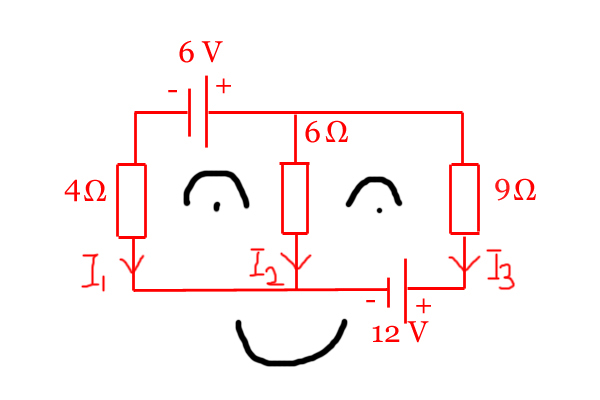
\includegraphics[scale = 0.4]{circuit.jpg}}
\caption{The circuit for Exercise \ref{ex:circuitsys}}
\label{fig:circuitsys}
\end{figure}\\
You will obtain two equations by considering any two loops with Kirchhoff’s Second Law, and one from Kirchhoff's First Law. So, there are three equations, for the three unknown currents.
\end{Exercise}
\begin{Answer}
The first two equations below come from the left inner loop and right inner loop, but one of them can be replaced by the outer loop as well.
\begin{align*}
-4I_1 + 6I_2 &= 6\\
-6I_2 + 9I_3 &= -12\\
I_1 + I_2 + I_3 &= 0
\end{align*}
and the solution is $I_1 = -\frac{3}{19}$, $I_2 = \frac{17}{19}$, $I_3 = -\frac{14}{19}$ (in Amperes).
\end{Answer}

\begin{Exercise}
\label{ex:shallowwater}
The \textit{shallow water equations} (see Figure \ref{fig:shallowwater}) describe the evolution of gravity wave under some approximations such as \textit{hydrostatic balance} and a sufficiently shallow fluid depth, and has the form of
\begin{align*}
\begin{dcases}
\frac{\partial \eta}{\partial t} + H(\frac{\partial u}{\partial x} + \frac{\partial v}{\partial y}) &= 0 \\
\frac{\partial u}{\partial t} &= -g\frac{\partial \eta}{\partial x} \\
\frac{\partial v}{\partial t} &= -g\frac{\partial \eta}{\partial y} 
\end{dcases}
\end{align*}
when the Coriolis effect is ignored. By assuming a travelling wave solution
\begin{align*}
u &= \tilde{U} \cos(kx + ly - \omega t) \\
v &= \tilde{V} \cos(kx + ly - \omega t) \\
\eta &= \tilde{\eta} \cos(kx + ly - \omega t)
\end{align*}
where $\tilde{U}$, $\tilde{V}$, $\tilde{\eta}$ are some constants to be determined, show that the equations become
\begin{align*}
\begin{dcases}
\omega \tilde{\eta} - kH \tilde{U} - lH \tilde{V} &= 0 \\
\omega \tilde{U} - kg \tilde{\eta} &= 0 \\
\omega \tilde{V} - lg \tilde{\eta} &= 0
\end{dcases}
\end{align*}
By requiring that $\tilde{U}$, $\tilde{V}$, $\tilde{\eta}$ have a non-trivial solution so that they are not all zeros, derive the dispersion relation of gravity wave, which is
\begin{align*}
\omega^2 &= gH(k^2 + l^2) \\
\omega &= c\kappa
\end{align*}
where $c = \sqrt{gH}$ is the wave speed, and $\kappa = \sqrt{k^2 + l^2}$ is the total wavenumber.
\end{Exercise}
\begin{figure}
\centering
\begin{tikzpicture}
    \draw [thick,color=black,domain=0:3*pi,samples=500] plot (\x, {5+0.5*sin(deg(4*\x))});
    \fill [blue!30] (3*pi,0) -- (0,0) -- plot[domain=0:3*pi,samples=500]  (\x, {5+0.5*sin(deg(4*\x))});
    \draw [thick,color=black] (0,0) -- (3*pi, 0);
    \fill [Brown!50!Orange] (0,0) rectangle (3*pi, -1) node[above left, black]{Bottom};
    \draw [<->] (3*pi+0.2, 0) -- (3*pi+0.2, 5) node[midway, xshift=8]{$H$};
    \draw [<->,red] (0.575*pi, 5.6) -- (0.575*pi, 5) node[midway, xshift=-8]{$\eta$};
    \draw [dashed, black] (0, 5) -- (3*pi, 5);
    \draw [thick, Green] (0.575*pi, 5) -- (0.575*pi, 0) node[midway, xshift=-8]{$u$};
    \draw [thick, Green, ->] (0.575*pi, 4) -- (0.575*pi+1, 4);
    \draw [thick, Green, ->] (0.575*pi, 3) -- (0.575*pi+1, 3);
    \draw [thick, Green, ->] (0.575*pi, 2) -- (0.575*pi+1, 2);
    \draw [thick, Green, ->] (0.575*pi, 1) -- (0.575*pi+1, 1);
    \node at (8.75, 2.5) {Fluid};
\end{tikzpicture}
\caption{The $x$-$z$ cross-section of shallow water system in Exercise \ref{ex:shallowwater}. $\eta$ is the height of free surface, $H$ is the mean depth of the fluid, and $u$ is the fluid velocity along $x$-axis.}
\label{fig:shallowwater}
\end{figure}
\begin{Answer}
Substituting the given wave solution forms into the equation, we have
\begin{align*}
\begin{split}
&\omega\tilde{\eta}\sin(kx+ly-\omega t) + H(-k\tilde{U}\sin(kx+ly-\omega t) \\
& -l\tilde{V}\sin(kx+ly-\omega t)) = 0 \\    
\end{split} \\
& \omega\tilde{U}\sin(kx+ly-\omega t) = gk\tilde{\eta}\sin(kx+ly-\omega t) \\
& \omega\tilde{V}\sin(kx+ly-\omega t) = gl\tilde{\eta}\sin(kx+ly-\omega t)
\end{align*}
Cancelling out all the sine factors, we arrive at the linear system displayed in the question
\begin{align*}
\begin{dcases}
\omega \tilde{\eta} - kH \tilde{U} - lH \tilde{V} &= 0 \\
\omega \tilde{U} - kg \tilde{\eta} &= 0 \\
\omega \tilde{V} - lg \tilde{\eta} &= 0
\end{dcases}
\end{align*}
For $\tilde{U}$, $\tilde{V}$, $\tilde{\eta}$ to have a non-trivial solution other than all zeros, we require the determinant of the corresponding coefficient matrix to be zero according to Theorem \ref{thm:sqlinsysunique}, which leads to
\begin{align*}
\begin{vmatrix}
\omega & -kH & -lH \\
-kg & \omega & 0 \\
-lg & 0 & \omega
\end{vmatrix} &= 0 \\
\omega^3 - gHk^2\omega - gHl^2\omega &= 0 \\
\omega^2 - gH(k^2 + l^2) &= 0 
\end{align*}
as the dispersion relation of gravity wave.
\end{Answer}

\begin{Exercise}
Solve for the condensation height and temperature $z_{cd}$ and $T_{cd}$ in Exercise \ref{ex:lapse}.
\end{Exercise}
\begin{Answer}
$T_{cd} \approx \SI{15.9}{\celsius}$, $z_{cd} \approx \SI{0.97}{\km}$.
\end{Answer}

\begin{Exercise}
Solve the \textit{Chickens and Rabbits in the Same Cage} problem in Exercise \ref{ex:animals}. If we now introduce a new type of mystical creature who has one head and three legs, and throw them in another cage along with some chickens and rabbits, find all possible numbers of the three species if the cage now has $48$ heads and $122$ legs.
\end{Exercise}
\begin{Answer}
$x = 23$, $y = 12$. For the extra part, the new system of equations become (denote the number of third species as $z$)
\begin{align*}
\begin{bmatrix}
1 & 1 & 1 \\
2 & 4 & 3
\end{bmatrix}
\begin{bmatrix}
x \\
y \\
z
\end{bmatrix}
=
\begin{bmatrix}
48 \\
122
\end{bmatrix}
\end{align*}
By Gaussian Elimination, we have
\begin{align*}
\left[
\begin{array}{@{}ccc|c@{}}
1 & 1 & 1 & 48 \\
2 & 4 & 3 & 122
\end{array}
\right]
&\to
\left[
\begin{array}{@{}ccc|c@{}}
1 & 1 & 1 & 48 \\
0 & 2 & 1 & 26
\end{array}
\right] & R_2 - 2R_1 \to R_2 \\
&\to
\left[
\begin{array}{@{}ccc|c@{}}
1 & 1 & 1 & 48 \\
0 & 1 & \frac{1}{2} & 13
\end{array}
\right] & \frac{1}{2}R_2 \to R_2 \\
&\to
\left[
\begin{array}{@{}ccc|c@{}}
1 & 0 & \frac{1}{2} & 35 \\
0 & 1 & \frac{1}{2} & 13
\end{array}
\right] & R_1 - R_2 \to R_1
\end{align*}
Let $z = t$ as the free variable, then we have $y = 13 - \frac{1}{2}t$ and $x = 35-\frac{1}{2}t$, and hence
\begin{align*}
\begin{bmatrix}
x \\
y \\
z
\end{bmatrix}
=
\begin{bmatrix}
35-\frac{1}{2}t \\
13-\frac{1}{2}t \\
t
\end{bmatrix}
=
\begin{bmatrix}
35 \\
13 \\
0
\end{bmatrix}
+
t
\begin{bmatrix}
-\frac{1}{2} \\
-\frac{1}{2} \\
1
\end{bmatrix}
\end{align*}
Since the numbers of species must be a non-negative integer, the solution can be expressed in a more good-looking form of
\begin{align*}
\begin{bmatrix}
x \\
y \\
z
\end{bmatrix}
=
\begin{bmatrix}
35 \\
13 \\
0
\end{bmatrix}
+
s
\begin{bmatrix}
-1 \\
-1 \\
2
\end{bmatrix}
\end{align*}
where $s = \frac{t}{2}$, and the range of $s$ is $0, 1, \ldots, 13$ (when $s$ reaches $13$ there is no chicken remained).
\end{Answer}
\chapter{Introduction to Vectors}

After three chapters of discussion about matrices, it is time to talk about another closely related object type in linear algebra, namely, vectors. While \textit{vectors} and \textit{vector spaces} have strictly mathematical definitions which make them abstract, we will take a more physical point of view with the special case of (finite-dimensional) geometric vectors first.

\section{Definition and Operations of Geometric Vectors}

\subsection{Basic Structure of Vectors in the Real $n$-space $\mathbb{R}^n$}
A \index{Vector}\index{Vector!Geometric Vector}\keywordhl{(geometric) vector} is a physical quantity represented by an ordered tuple of \textit{components} (numbers), e.g. $(1, 8, 7, 4)$, $(1-\imath, 1+3\imath, 2)$. It has a \textit{magnitude (length)} and \textit{direction}, resembling an arrow. Some real-life examples are: two-dimensional flow velocity $(u, v)$, the relative position of an airplane to a ground radar $(x, y, z)$.
\begin{defn}[$n$-dimensional Geometric Vector]
\label{defn:geometvec}
A $n$-dimensional geometric vector consists of $n$ ordered numbers called \index{Components}\keywordhl{components} and are denoted by either an arrow or boldface, like $\vec{v}$ or $\textbf{v}$. It is usually written out in two forms, as a \textit{column vector} or an \textit{ordered $n$-tuple}:
\begin{align*}
\vec{v} &=
\begin{bmatrix}
v_1 \\
v_2 \\
v_3 \\
\vdots \\
v_n
\end{bmatrix}
=
(v_1, v_2, v_3, \ldots, v_n)^T
\end{align*}
\end{defn}
A $n$-dimensional vector can be treated as an $n \times 1$ (\index{Vector!Column Vector}\keywordhl{column vector}) as suggested above, or a $1 \times n$ matrix (\index{Vector!Row Vector}\keywordhl{row vector}) depending on the situation. The form of a column vector is taken more often than the row vector one and so the column form is assumed throughout the book if it is not further specified. That is why the superscript $^T$ is added for the $n$-tuple form to reflect that it is in fact a column vector despite written horizontally. \par
\begin{tikzpicture}
\draw[->] (-2.5,0)--(2.5,0) node[right]{$x$};
\draw[->] (0,-2.5)--(0,2.5) node[above]{$y$};
\draw[blue,->,line width=1.2] (0,0)--(2,1) node[anchor=south]{$\vec{v} = (2,1)^T$};
\draw[Gray,dashed] (2,1)--(2,0) node[below]{$x = 2$};
\draw[Gray,dashed] (2,1)--(0,1) node[left]{$y = 1$};
\node[below left]{$O$}; 
\end{tikzpicture}\\    
A 2D vector drawn in an x-y plane.\par
{\fbox{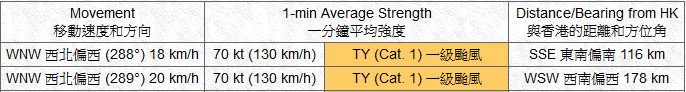
\includegraphics[scale = 0.5]{higos.jpg}}\\
Forecast for \textit{Typhoon Higos} (taken from \href{http://www.hkww.org/weather/tcarchive.html}{Hong Kong Weather Watch}). Its horizontal movement is a two-dimensional vector, even though the speed and direction are given instead of the velocities in $x$ and $y$-direction (they can be converted to each other).}

Implicit in the definition of $n$-dimensional vectors is the $n$-dimensional \textit{space} they are residing in. Assume the components of those vectors are all real, then the set of all such vectors constitutes the \index{Real $n$-space}\keywordhl{real $n$-space $\mathbb{R}^n$}.
\begin{defn}[The Real $n$-space $\mathbb{R}^n$]
\label{defn:real_nspace}
The real $n$-space $\mathbb{R}^n$ is defined as the set of all possible $n$-tuples $\vec{v} = (v_1, v_2, v_3, \ldots, v_n)^T$ as defined in Definition \ref{defn:geometvec}, where $v_i$ can take any \textit{real} value, for $i = 1,2,3,\ldots,n$. Such objects in $\mathbb{R}^n$ are known as $n$-dimensional \textit{real} vectors.
\end{defn}
While we have not clearly defined what a vector space is, we note that $\mathbb{R}^n$ fulfills the requirements of a vector space in a mathematical sense. A more detailed discussion of this aspect will be deferred to Chapter \ref{chap:vec_space}. Meanwhile, the complex counterpart will be explored in Chapter \ref{chap:complex}.\\
\\
An $n$-dimensional real geometric vector as described in Definition \ref{defn:geometvec} and \ref{defn:real_nspace} can be written as the sum of $n$ \index{Standard Unit Vector}\keywordhl{standard unit vectors} that have a magnitude of $1$ and are oriented in the positive direction along the $p$-th coordinates axes. They are denoted by $\hat{e}_p$, where $p$ can be from $1$ to $n$. The coordinate axes are perpendicular (or more generally, \textit{orthogonal}, introduced later in this chapter) to each other and this coordinate system is known as the \index{Cartesian Coordinate System}\keywordhl{Cartesian (coordinate) system}. Particularly, in the three-dimensional real space $\mathbb{R}^3$, $\hat{e}_1 = \hat{i} = (1,0,0)^T$, $\hat{e}_2 = \hat{j} = (0,1,0)^T$, $\hat{e}_3 = \hat{k} = (0,0,1)^T$ correspond to "an arrow" of length $1$ pointing in the positive direction of the $x$, $y$, $z$ axes respectively. 
\begin{defn}[Standard Unit Vector]
\label{defn:standardunitvec}
A standard unit vector $\hat{e}_p$ in the real $n$-space $\mathbb{R}^n$ (Definition \ref{defn:real_nspace}) has $n$ components, consisted of $1$ at the $p$-th entry and $0$ elsewhere. Mathematically, for $1\leq q \leq n$, $[\hat{e}_p]_q = 1$ when $q=p$ and $[\hat{e}_p]_q = 0$ when $q\neq p$.
\end{defn}
Below is an example of a geometric vector in the three-dimensional $xyz$ space ($\mathbb{R}^3$).
\begin{center}
\begin{tikzpicture}[x={(1.8cm, -0.4cm)}, y={(1.4cm, 1.2cm)}, z={(0cm, 2cm)}]
\draw [->] (0,0,0) -- (2,0,0) node [below right] {$x$};
\draw [->] (0,0,0) -- (0,2,0) node [above] {$y$};
\draw [->] (0,0,0) -- (0,0,2) node [left] {$z$};
\draw [->, thick, red, line width=1] (0,0,0) -- (1,0,0) node [below left] {$\hat{i} = (1,0,0)^T$};
\draw [->, thick, red, line width=1] (0,0,0) -- (0,1,0) node [above right, midway, sloped] {$\hat{j} = (0,1,0)^T$} ; 
\draw [->, thick, red, line width=1] (0,0,0) -- (0,0,1) node [left] {$\hat{k} = (0,0,1)^T$};
\draw [Gray, dashed] (1.8,0.4,0) -- (1.8,0,0) node[right, midway]{$y=0.4$}; 
\draw [Gray, dashed] (1.8,0.4,0) -- (0,0.4,0) node[above, midway, sloped]{$x=1.8$}; 
\draw [Gray, dashed] (1.8,0.4,0) -- (1.8,0.4,1.1) node[midway, right]{$z=1.1$};
\draw [->, blue, line width=1.2] (0,0,0) -- (1.8,0.4,1.1) node [right] {$\vec{v} = (1.8,0.4,1.1)^T$};
/\end{tikzpicture}
\begin{align*}
\vec{v} &= 
\begin{bmatrix}
1.8 \\
0.4 \\
1.1
\end{bmatrix}
= 1.8
\begin{bmatrix}
1 \\
0 \\
0
\end{bmatrix}
+ 0.4
\begin{bmatrix}
0 \\
1 \\
0
\end{bmatrix}
+ 1.1
\begin{bmatrix}
0 \\
0 \\
1
\end{bmatrix} 
= 1.8\hat{i} + 0.4\hat{j} + 1.1\hat{k} \\
&= (1.8,0.4,1.1)^T
\end{align*}
\end{center}
where we have written $\vec{v}$ in two forms, as an $n$-tuple and a sum of the three standard unit vectors $\hat{i}, \hat{j}, \hat{k}$.

\subsection{Fundamental Vector Operations}
\label{section:vectoraddmul}
\subsubsection{Addition and Subtraction}
Same as their matrix counterpart, addition and subtraction between vectors are component-wise, and hence only valid for vectors of the same dimension. For $\vec{w} = \vec{u} \pm \vec{v}$, we have $w_i = u_i \pm v_i$. If
\begin{align*}
&\vec{u} =
\begin{bmatrix}
1 \\
2
\end{bmatrix}
&
\vec{v} =
\begin{bmatrix}
2 \\
-1
\end{bmatrix}
\end{align*}
then
\begin{align*}
\vec{u} + \vec{v} =
\begin{bmatrix}
\textcolor{red}{1} \\
\textcolor{red}{2}
\end{bmatrix}
+
\begin{bmatrix}
\textcolor{blue}{2} \\
\textcolor{blue}{-1}
\end{bmatrix}
&= 
\begin{bmatrix}
\textcolor{Green}{3} \\
\textcolor{Green}{1}
\end{bmatrix}
\\
\vec{u} - \vec{v} =
\begin{bmatrix}
\textcolor{red}{1} \\
\textcolor{red}{2}
\end{bmatrix}
-
\begin{bmatrix}
\textcolor{blue}{2} \\
\textcolor{blue}{-1}
\end{bmatrix}
&= 
\begin{bmatrix}
\textcolor{Green}{-1} \\
\textcolor{Green}{3}
\end{bmatrix}
\end{align*}
\begin{center}
\begin{tikzpicture}[scale=0.8]
\draw[->] (-3.5,0)--(3.5,0) node[right]{$x$};
\draw[->] (0,-3.5)--(0,3.5) node[above]{$y$};
\draw[red,-stealth,line width=1] (0,0)--(1,2) node[anchor=south west]{$\vec{u} = (1,2)^T$};
\draw[blue,-stealth,line width=1] (1,2)--(3,1) node[anchor=south west]{$\vec{v} = (2,-1)^T$};
\draw[Green,-stealth,line width=1] (0,0)--(3,1) node[anchor=north west]{$\vec{u} + \vec{v} = (3,1)^T$};
\node[below left]{$O$}; 
\end{tikzpicture}\\
Addition: The tail of the blue vector is placed to the head of the red vector, and the resultant green vector is from the origin to the head of blue vector.
\end{center}
\begin{center}
\begin{tikzpicture}[scale=0.8]
\draw[->] (-3.5,0)--(3.5,0) node[right]{$x$};
\draw[->] (0,-3.5)--(0,3.5) node[above]{$y$};
\draw[red,-stealth,line width=1] (0,0)--(1,2) node[anchor=south west]{$\vec{u} = (1,2)^T$};
\draw[blue,-stealth,line width=1] (1,2)--(-1,3) node[anchor=south east]{$-\vec{v} = (-2,1)^T$};
\draw[Green,-stealth,line width=1] (0,0)--(-1,3) node[anchor=north east]{$\vec{u} - \vec{v} = (-1,3)^T$};
\node[below left]{$O$}; 
\end{tikzpicture}\\
Subtraction: Similar to addition but with the blue vector oriented in the opposite direction.
\end{center}

\subsubsection{Scalar Multiplication} 
Multiplying a scalar (be it a real or complex number) to a vector means that all components are multiplied by that scalar.
\begin{align*}
2
\begin{bmatrix}
2 \\
0 \\
1 \\
9
\end{bmatrix}
=
\begin{bmatrix}
4 \\
0 \\
2 \\
18
\end{bmatrix}
\end{align*}
Looking back at vector subtraction, it can be viewed as addition with a factor of $-1$ in the front.
\begin{align*}
\begin{bmatrix}
7 \\
5 \\
9
\end{bmatrix}
-
\begin{bmatrix}
3 \\
6 \\
9
\end{bmatrix}
=
\begin{bmatrix}
7 \\
5 \\
9
\end{bmatrix}
+ (-1)
\begin{bmatrix}
3 \\
6 \\
9
\end{bmatrix}
=
\begin{bmatrix}
7 \\
5 \\
9
\end{bmatrix}
+
\begin{bmatrix}
-3 \\
-6 \\
-9
\end{bmatrix}
=
\begin{bmatrix}
4 \\
-1 \\
0
\end{bmatrix}
\end{align*}

\subsubsection{Length and Unit Vector} \index{Length}\index{Magnitude}\keywordhl{Length (magnitude)}, or more formally \index{Euclidean Norm}\keywordhl{Euclidean norm}, of a vector $\vec{v}$ is based on a generalized version of \index{Pythagoras' Theorem}\keywordhl{Pythagoras' Theorem}, and is evaluated as the square root of the sum of squares of components.
\begin{defn}[Vector Length]
\label{defn:vectorlength}
Length, or magnitude of a $n$-dimensional \textit{real} vector $\vec{v}$, denoted by $\norm{\vec{v}}$, is given by
\begin{align*}
\norm{\vec{v}} &= \sqrt{v_1^2 + v_2^2 + v_3^2 + \cdots + v_n^2} \\
&= \sqrt{\sum_{k=1}^{n} v_k^2}
\end{align*}
\end{defn}
For instance, the length of a two-dimensional vector follows the usual Pythagoras' Theorem as below. \\
\begin{tikzpicture}
\draw[->] (-2.5,0)--(2.5,0) node[right]{$x$};
\draw[->] (0,-2.5)--(0,2.5) node[above]{$y$};
\draw[blue,-stealth,line width=1.2] (0,0)--(2,1) node[anchor=south west, align=left]{$\vec{v} = (2,1)^T$\\$\norm{\vec{v}} = \sqrt{x^2 + y^2} = \sqrt{2^2+1^2} = \sqrt{5}$};
\draw[Gray,dashed] (2,1)--(2,0) node[below]{$x = 2$};
\draw[Gray,dashed] (2,1)--(0,1) node[left]{$y = 1$};
\node[below left]{$O$}; 
\end{tikzpicture}\\
Here is another example which is three-dimensional.
\begin{center}
\begin{tikzpicture}[x={(1.8cm, -0.6cm)}, y={(1.6cm, 1.0cm)}, z={(0cm, 2cm)}]
\draw [->] (-1,0,0) -- (2,0,0) node [right] {$x$};
\draw [->] (0,-1,0) -- (0,2,0) node [above] {$y$};
\draw [->] (0,0,0) -- (0,0,2) node [left] {$z$};
\node[below] (0,0,0){$O$};
\draw [Gray, dashed] (1.6,-0.2,0) -- (1.6,0,0) node[below, pos=-0.5, sloped]{$y=-1$}; 
\draw [Gray, dashed] (1.6,-0.2,0) -- (0,-0.2,0) node[below, midway, sloped]{$x=8$}; 
\draw [Gray, dashed] (1.6,-0.2,0) -- (1.6,-0.2,0.8) node[midway, right]{$z=4$};
\draw [->, blue, line width=1.2] (0,0,0) -- (1.6,-0.2,0.8) node [right] {$\vec{w} = (8,-1,4)^T$};
\end{tikzpicture}
\begin{align*}
\vec{w} &= 
\begin{bmatrix}
8 \\
-1 \\
4
\end{bmatrix}
& \norm{\vec{w}}&=
\sqrt{8^2 + (-1)^2 + 4^2} = 9 
\end{align*}
\end{center}
We can create a \index{Vector!Unit Vector}\keywordhl{unit vector} that has a length of $1$ from any vector $\vec{v}$ and orients in the same direction as $\vec{v}$. It is simply created by dividing (normalizing) $\vec{v}$ by its distance $\norm{\vec{v}}$.
\begin{defn}[Unit Vector]
\label{defn:unitvec}
The unit vector corresponding to a non-zero vector $\vec{v}$ is denoted as $\hat{v}$ and is given by
\begin{align*}
\hat{v} &= \frac{1}{\norm{\vec{v}}}\vec{v}
\end{align*}
where the length $\norm{\vec{v}}$ is defined as in Definition \ref{defn:vectorlength}. 
\end{defn}
Note that despite vectors can carry physical units, unit vectors are all physically \textit{dimensionless} when formulated in this way. \\
\\
Short Exercise: Find the unit vector for $\vec{w} = (8, -1, 4)^T$ in the previous example, and verify that it has a length of $1$.\footnote{$\norm{\vec{w}} = 9$, $\hat{w} = \frac{\vec{w}}{\norm{\vec{w}}} = \frac{1}{9}(8,-1,4)^T = (\frac{8}{9}, -\frac{1}{9}, \frac{4}{9})^T$, $\norm{\hat{w}} = \sqrt{(\frac{8}{9})^2 + (-\frac{1}{9})^2 + (\frac{4}{9})^2} = 1$.}

\section{Special Vector Operations}
\label{section:vectorops}
Now we are going to introduce two special types of vector operations: \textit{dot product}, and \textit{cross product}. 

\subsection{Dot Product}
\label{section:dotprod}
\index{Dot Product}\keywordhl{(Real) Dot product} (or \index{Scalar Product}\keywordhl{scalar product}) is defined for two (real) vectors that have the same number of dimension. It is the sum of products of paired components between the two vectors. In other words, it can be regarded to be the matrix product between a row vector ($1 \times m$ matrix) and a column vector ($m \times 1$ matrix). 
\begin{defn}[Dot Product (Real)]
\label{defn:dotreal}
The dot product between two $n$-dimensional \textit{real} vectors $\vec{u}$ and $\vec{v}$ in $\mathbb{R}^n$ are denoted as either $\vec{u} \cdot \vec{v}$, or by matrix notation $\textbf{u}^T\textbf{v}$. They are defined as
\begin{align*}
\vec{u} \cdot \vec{v} = \textbf{u}^T\textbf{v} &= u_1v_1 + u_2v_2 + u_3v_3 + \cdots + u_nv_n \\
&= \sum_{k=1}^{n} u_kv_k
\end{align*}
which is a scalar quantity.
\end{defn}
Conversely, it can be said that entries of a matrix product are vector dot products between the corresponding rows and columns. It is emphasized that we are restricting ourselves to real entries since complex vectors introduce a bit of extra complications. Then, for two \textit{real} matrices expressed in the form of combined row/column vectors that are $\mathbb{R}^n$,
\begin{align*}
A &= \left[\begin{array}{@{}c@{}}
\text{---} \vec{u}^{(1)T} \text{---} \\
\hline
\text{---} \vec{u}^{(2)T} \text{---} \\
\hline
\vdots \\
\hline
\text{---} \vec{u}^{(p)T} \text{---}
\end{array}\right]
=  \left[\begin{array}{@{}c|c|c|c@{}}
| & | & & | \\
\vec{u}^{(1)} & \vec{u}^{(2)} & \cdots & \vec{u}^{(p)} \\
| & | & & |
\end{array}\right]^T
& B &= \left[\begin{array}{@{}c|c|c|c@{}}
| & | & & | \\
\vec{v}^{(1)} & \vec{v}^{(2)} & \cdots & \vec{v}^{(q)} \\
| & | & & |
\end{array}\right]\\
&= 
\begin{bmatrix}
\vec{u}^{(1)}_1  & \vec{u}^{(1)}_2 & \cdots & \vec{u}^{(1)}_n \\
\vec{u}^{(2)}_1  & \vec{u}^{(2)}_2 & \cdots & \vec{u}^{(2)}_n \\
\vdots & \vdots & & \vdots \\
\vec{u}^{(p)}_1  & \vec{u}^{(p)}_2 & \cdots & \vec{u}^{(p)}_n
\end{bmatrix} 
& &= 
\begin{bmatrix}
\vec{v}^{(1)}_1  & \vec{v}^{(2)}_1 & \cdots & \vec{v}^{(q)}_1 \\
\vec{v}^{(1)}_2  & \vec{v}^{(2)}_2 & & \vec{v}^{(q)}_2 \\
\vdots & & \ddots & \vdots \\
\vec{v}^{(1)}_n  & \vec{v}^{(2)}_n & \cdots & \vec{v}^{(q)}_n \\
\end{bmatrix} 
\end{align*}
(notice those transposes in the expression of $A$) their matrix product $AB$ can be written as
\begin{align*}
AB =
\begin{bmatrix}
\vec{u}^{(1)} \cdot \vec{v}^{(1)} & \vec{u}^{(1)} \cdot \vec{v}^{(2)} & \cdots & \vec{u}^{(1)} \cdot \vec{v}^{(q)} \\
\vec{u}^{(2)} \cdot \vec{v}^{(1)} & \vec{u}^{(2)} \cdot \vec{v}^{(2)} & \cdots & \vec{u}^{(2)} \cdot \vec{v}^{(q)} \\
\vdots & \vdots & & \vdots \\
\vec{u}^{(p)} \cdot \vec{v}^{(1)} & \vec{u}^{(p)} \cdot \vec{v}^{(2)} & \cdots & \vec{u}^{(p)} \cdot \vec{v}^{(q)} \\
\end{bmatrix}
\end{align*}
We can use dot product to express the length of a real vector.
\begin{proper}
\label{proper:lengthdot}
The length of a real vector, as defined in Definition \ref{defn:vectorlength}, can be written using its dot product between itself as
\begin{align*}
\norm{\vec{v}} &= \sqrt{\vec{v} \cdot \vec{v}} & &\text{or} &
\norm{\vec{v}}^2 &= \vec{v} \cdot \vec{v}
\end{align*}
\end{proper}
Notice that $\vec{v} \cdot \vec{v} = v_1^2 + v_2^2 + v_3^2 + \cdots + v_n^2 \geq 0$. This quantity is always strictly greater than zero ($\vec{v} \cdot \vec{v} > 0$) unless $\vec{v} = \textbf{0}$ is the zero vector (then $\vec{v} \cdot \vec{v} = 0$), which makes sense physically given that it represents length.

\begin{exmp}
\label{exmp:dotproduct5d}
If $\vec{u} = (1, 2, 3, 4, 5)^T$ and $\vec{v} = (-1, 0, 2, 1, -2)^T$, find the dot product $\vec{u} \cdot \vec{v} = \textbf{u}^T\textbf{v}$.
\end{exmp}
\begin{solution}
\begin{align*}
\vec{u} \cdot \vec{v} &= (1)(-1) + (2)(0) + (3)(2) + (4)(1) + (5)(-2) = -1
\end{align*}
Alternatively,
\begin{align*}
\textbf{u}^T\textbf{v} &=
\begin{bmatrix}
1 & 2 & 3 & 4 & 5
\end{bmatrix}
\begin{bmatrix}
-1 \\
0 \\
2 \\
1 \\
-2
\end{bmatrix}
= -1
\end{align*}
\end{solution}

Here are some properties of dot product.
\begin{proper}
\label{proper:dotproper}
For three $n$-dimensional real vectors $\vec{u}$, $\vec{v}$ and $\vec{w}$, the following properties hold.
\begin{align*}
\vec{u} \cdot \vec{v} &= \vec{v} \cdot \vec{u} &\text{Symmetry Property} \\
\vec{u} \cdot (\vec{v} \pm \vec{w}) &= \vec{u} \cdot \vec{v} \pm \vec{u} \cdot \vec{w} &\text{Distributive Property} \\
(\vec{u} \pm \vec{v}) \cdot \vec{w} &= \vec{u} \cdot \vec{w} \pm \vec{v} \cdot \vec{w} &\text{Distributive Property} \\
(a\vec{u}) \cdot (b\vec{v}) &= ab(\vec{u} \cdot \vec{v}) &\text{where $a$, $b$ are some constants}
\end{align*}
Additionally, if $A$ is an $n \times n$ square matrix, then
\begin{align*}
\vec{u} \cdot (A\vec{v}) &= \textbf{u}^T(A\textbf{v}) = (A^T\textbf{u})^T\textbf{v} = (A^T\vec{u}) \cdot \vec{v} \\
(A\vec{u}) \cdot \vec{v} &= (A\textbf{u})^T\textbf{v} = \textbf{u}^T(A^T\textbf{v}) = \vec{u} \cdot (A^T\vec{v})
\end{align*}
where we have used Definition \ref{defn:dotreal} and Properties \ref{proper:transp}.
\end{proper}
\begin{exmp}
For $\vec{u} = (1,3,1)^T$ and $\vec{v} = (2,-1,1)^T$, find $\norm{(\vec{u} + \vec{v})}^2 = (\vec{u} + \vec{v}) \cdot (\vec{u} + \vec{v})$.
\end{exmp}
\begin{solution}
By Properties \ref{proper:dotproper}, we can rewrite the expression as
\begin{align*}
(\vec{u} + \vec{v}) \cdot (\vec{u} + \vec{v}) &= \vec{u} \cdot (\vec{u} + \vec{v}) + \vec{v} \cdot (\vec{u} + \vec{v}) \\
&= \vec{u} \cdot \vec{u} + \vec{u} \cdot \vec{v} + \vec{v} \cdot \vec{u} + \vec{v} \cdot \vec{v} \\
&= \vec{u} \cdot \vec{u} + 2 \vec{u} \cdot \vec{v} + \vec{v} \cdot \vec{v}
\end{align*}
Subsequently,
\begin{align*}
&\quad \vec{u} \cdot \vec{u} + 2 \vec{u} \cdot \vec{v} + \vec{v} \cdot \vec{v} \\
&= (1,3,1)^T \cdot (1,3,1)^T + 2((1,3,1)^T \cdot (2,-1,1)^T) + (2,-1,1)^T \cdot (2,-1,1)^T \\
&= (1^2 + 3^2 + 1^2) + 2((1)(2)+(3)(-1)+(1)(1)) + (2^2 + (-1)^2 + 1^2) \\
&= 11 + 2(0) + 6 \\
&= 17
\end{align*}
Alternatively, one can calculate $\vec{w} = \vec{u} + \vec{v} = (1,3,1)^T + (2,-1,1)^T = (3,2,2)^T$ and find $\vec{w} \cdot \vec{w} = \norm{\vec{w}}^2$ instead. (which is easier and faster)
\end{solution}
\begin{exmp}
Given $\vec{u}$ and $\vec{v}$ as defined in the example above, if
\begin{align*}
A =
\begin{bmatrix}
1 & 2 & 1 \\
2 & 0 & 3 \\
1 & 1 & -1
\end{bmatrix}
\end{align*}
verify that $\vec{u} \cdot (A\vec{v}) = (A^T\vec{u}) \cdot \vec{v}$.
\end{exmp}
\begin{solution}
\begin{align*}
A\vec{v} &= 
\begin{bmatrix}
1 & 2 & 1 \\
2 & 0 & 3 \\
1 & 1 & -1
\end{bmatrix}
\begin{bmatrix}
2 \\
-1 \\
1
\end{bmatrix} \\
&=
\begin{bmatrix}
(1)(2) + (2)(-1) + (1)(1) \\
(2)(2) + (0)(-1) + (3)(1) \\
(1)(2) + (1)(-1) + (-1)(1) 
\end{bmatrix} \\
&=
\begin{bmatrix}
1 \\
7 \\
0
\end{bmatrix} \\
\vec{u} \cdot (A\vec{v}) &= (1,3,1)^T \cdot (1,7,0)^T \\
&= (1)(1) + (3)(7) + (1)(0) \\
&= 22
\end{align*}
On the other hand,
\begin{align*}
A^T\vec{u} &= 
\begin{bmatrix}
1 & 2 & 1 \\
2 & 0 & 1 \\
1 & 3 & -1
\end{bmatrix}
\begin{bmatrix}
1 \\
3 \\
1
\end{bmatrix} \\
&=
\begin{bmatrix}
(1)(1) + (2)(3) + (1)(1) \\
(2)(1) + (0)(3) + (1)(1) \\
(1)(1) + (3)(3) + (-1)(1) 
\end{bmatrix} \\
&=
\begin{bmatrix}
8 \\
3 \\
9
\end{bmatrix} \\
(A^T\vec{u}) \cdot \vec{v} &= (8,3,9)^T \cdot (2,-1,1)^T \\
&= (8)(2) + (3)(-1) + (9)(1) \\
&= 22
\end{align*}
\end{solution}

\subsubsection{Geometric Meaning of Dot Product}
The geometric meaning of dot product is embedded in the relation below.
\begin{proper}
\label{proper:dotgeo}
For two real vectors $\vec{u}$ and $\vec{v}$ that are of the same dimension, we have
\begin{align*}
\vec{u} \cdot \vec{v} = \norm{\vec{u}}\norm{\vec{v}}\cos\theta
\end{align*}
where $\theta$ is the angle between $\vec{u}$ and $\vec{v}$. Furthermore, if $\hat{u}$ and $\hat{v}$ are unit vectors (Definition \ref{defn:unitvec}) such that $\norm{\vec{u}} = \norm{\vec{v}} = 1$, it reduces to
\begin{align*}
\hat{u} \cdot \hat{v} = \cos\theta    
\end{align*}
\end{proper}
This means that the dot product between two vectors $\vec{u}$ and $\vec{v}$ is geometrically the signed product between $\vec{u}$ and the parallel component (projection) of $\vec{v}$ onto $\vec{u}$ (or vice versa), which is illustrated in the figure below. While an angle has a clear physical meaning only in a two/three-dimensional space, such relation generalizes the idea of an angle to higher dimensions.
\begin{center}
\begin{tikzpicture}[scale=1.3]
\coordinate (0) at (0,0);
\coordinate (vecu) at (4,1);
\coordinate (vecv) at (1,2);
\draw[->](0)--(vecu) node[right]{$\vec{u}$};
\draw[->](0)--(vecv) node[above]{$\vec{v}$};
\draw[dashed] (1,2)--(24/17, 6/17);
\draw[red] (24/17+0.2, 6/17+0.05)--(24/17+0.15, 6/17+0.25)--(24/17-0.05, 6/17+0.2);
\pic[draw, "$\theta$", angle eccentricity=1.5] {angle = vecu--0--vecv};
\draw[blue, very thick] (0,0)--(24/17, 6/17) node[below, shift={(0mm, -2mm)}]{$\norm{\vec{v}}\cos\theta$};
\end{tikzpicture}
\end{center}
\begin{exmp}
Find the angle between $\vec{u}$ and $\vec{v}$ in Example \ref{exmp:dotproduct5d}.
\end{exmp}
\begin{solution}
From Example \ref{exmp:dotproduct5d}, we have $\vec{u} \cdot \vec{v} = -1$, and
\begin{align*}
\norm{\vec{u}} &= \sqrt{1^2 + 2^2 + 3^2 + 4^2 + 5^2} = \sqrt{55} \\
\norm{\vec{v}} &= \sqrt{(-1)^2 + 0^2 + 2^2 + 1^2 + (-2)^2} = \sqrt{10} 
\end{align*}
By Properties \ref{proper:dotgeo}, we have
\begin{align*}
\cos\theta &= \frac{\vec{u} \cdot \vec{v}}{\norm{\vec{u}}\norm{\vec{v}}} \\
&= \frac{-1}{(\sqrt{55})(\sqrt{10})} \\
&\approx -0.0426 \\
\theta &\approx \SI{1.613}{\radian} = \SI{92.44}{\degree}
\end{align*}
\end{solution}
By Properties \ref{proper:dotgeo}, if the absolute value of the dot product $|\vec{u} \cdot \vec{v}|$ is equal to $\norm{\vec{u}}\norm{\vec{v}}$, where $\vec{u}$ and $\vec{v}$ are non-zero vectors, then it implies that $\cos\theta = \pm 1$, $\theta$ is either $0$ or $\pi$, and hence the two vectors are parallel. In constrast,
\begin{proper}
\label{proper:dotorth}
If the dot product between two real vectors $\vec{u}$ and $\vec{v}$ is zero ($\vec{u} \cdot \vec{v} = \vec{v} \cdot \vec{u} = 0$), then by Properties \ref{proper:dotgeo}, $\cos\theta = 0$ and the angle $\theta$ between $\vec{u}$ and $\vec{v}$ is $\frac{\pi}{2}$. In this case, $\vec{u}$ and $\vec{v}$ are said to be perpendicular, or \textit{orthogonal} to each other.
\end{proper}
From this, the concept of "\index{Orthogonal}\keywordhl{orthogonal}" becomes an extension of "perpendicular" in higher dimensions. It is easy to see that the standard unit vectors of $\mathbb{R}^n$ are orthogonal. Note that \textit{the zero vector is regarded to be orthogonal to any vector}, so even if $\vec{u}$ or $\vec{v}$ is a zero vector, this properties still hold. \par
Some may notice that as $-1 \leq \cos\theta \leq 1$, if $|\vec{u} \cdot \vec{v}| > \norm{\vec{u}}\norm{\vec{v}}$, then $\theta$ in Properties \ref{proper:dotgeo} will be ill-defined. However, the \index{Cauchy–Schwarz Inequality}\keywordhl{Cauchy–Schwarz Inequality} ensures this will not happen.
\begin{thm}[Cauchy–Schwarz Inequality]
\label{thm:CauchySch}
Given two \textit{real} $n$-dimensional vectors $\vec{u}$ and $\vec{v}$ ($\vec{u}, \vec{v} \in \mathbb{R}^n$), the following inequality holds.
\begin{align*}
|\vec{u} \cdot \vec{v}| &\leq \norm{\vec{u}}\norm{\vec{v}} \\
|u_1v_1+u_2v_2+\cdots+u_nv_n| &\leq \sqrt{u_1^2+u_2^2+\cdots+u_n^2}\sqrt{v_1^2+v_2^2+\cdots+v_n^2}
\end{align*}
\end{thm}
\begin{proof}
Consider $\vec{w} = \vec{u} + t\vec{v}$, where $t$ is any scalar, then $\norm{\vec{w}}^2 = \vec{w}\cdot\vec{w} \geq 0$ by Properties \ref{proper:lengthdot}. Also, $\vec{w}\cdot\vec{w}$ can be written as a quadratic polynomial in $t$:
\begin{align*}
\vec{w}\cdot\vec{w} = (\vec{u} + t\vec{v}) \cdot (\vec{u} + t\vec{v}) = \norm{\vec{u}}^2 + 2t(\vec{u} \cdot \vec{v}) + t^2\norm{\vec{v}}^2
\end{align*}
Since this quantity is always greater than or equal to zero, i.e.\ the quadratic polynomial has no root or a repeated root, it means that the discriminant must be negative or zero. So,
\begin{align*}
\Delta = b^2 - 4ac &\leq 0 \\
(2(\vec{u} \cdot \vec{v}))^2 - 4\norm{\vec{u}}^2\norm{\vec{v}}^2 &\leq 0 \\
(\vec{u} \cdot \vec{v})^2 - \norm{\vec{u}}^2\norm{\vec{v}}^2 &\leq 0 \\
(\vec{u} \cdot \vec{v})^2 &\leq \norm{\vec{u}}^2\norm{\vec{v}}^2 \\
|\vec{u} \cdot \vec{v}| &\leq \norm{\vec{u}}\norm{\vec{v}}
\end{align*}
\end{proof}
Short Exercise: Think about under what circumstances the Cauchy–Schwarz Inequality turns into an equality (i.e.\ $|\vec{u} \cdot \vec{v}| = \norm{\vec{u}}\norm{\vec{v}}$).\footnote{When $\vec{u}$ and $\vec{v}$ are parallel, i.e. $\vec{u} = k\vec{v}$ for some scalar $k$, or $\vec{v} = \textbf{0}$.}

\begin{exmp}
Prove the \index{Cosine Law}\keywordhl{Cosine Law} by considering the triangle below
\begin{center}
\begin{tikzpicture}
\coordinate (0) at (0,0);
\draw[red,-{Latex[length=5mm, width=2mm]}] (0)--(5,1) node[right](vecu){$\vec{u}$};
\draw[blue,-{Latex[length=5mm, width=2mm]}] (0)--(-1,3) node[above](vecv){$\vec{v}$};
\pic[draw, "$\theta$", angle eccentricity=1.5] {angle = vecu--0--vecv};
\draw[Green,-{Latex[length=5mm, width=2mm]}] (-1,3)--(5,1) node[midway, above, shift={(0mm, 3mm)}]{$\vec{u} - \vec{v}$};
\end{tikzpicture}
\end{center}
and expanding the dot product $\norm{(\vec{u}-\vec{v})}^2 = (\vec{u}-\vec{v}) \cdot (\vec{u}-\vec{v})$.    
\end{exmp}
\begin{solution}
Let denote the lengths $\norm{\vec{u}}$, $\norm{\vec{v}}$, $\norm{(\vec{u}-\vec{v})}$ be $a$, $b$, $c$, then
\begin{align*}
c^2 = \norm{(\vec{u}-\vec{v})}^2 &= (\vec{u}-\vec{v}) \cdot (\vec{u}-\vec{v}) & \text{(Properties \ref{proper:lengthdot})} \\
&= \vec{u} \cdot \vec{u} - \vec{u} \cdot \vec{v} - \vec{v} \cdot \vec{u} + \vec{v} \cdot \vec{v} & \text{(Properties \ref{proper:dotproper})} \\
&= \norm{\vec{u}}^2 - 2\vec{u} \cdot \vec{v} + \norm{\vec{v}}^2 & \text{(Properties \ref{proper:lengthdot} and \ref{proper:dotproper})} \\
&= \norm{\vec{u}}^2 - 2\norm{\vec{u}}\norm{\vec{v}}\cos\theta + \norm{\vec{v}}^2 & \text{(Properties \ref{proper:dotgeo})} \\
&= a^2 - 2ab\cos\theta + b^2
\end{align*}
\end{solution}

\subsection{Cross Product}
\label{section:crossprod}
Another important type of vector product is the \index{Cross Product}\keywordhl{cross product} (or sometimes just \index{Vector Product}\keywordhl{vector product}), which produces a three-dimensional real vector from two other three-dimensional real vectors. \textit{The output vector will be orthogonal to the two input vectors}, and the direction is determined by the \index{Right Hand Rule}\keywordhl{right hand rule}. Motivated by these requirements, we have the following basic definitions of cross product between the three standard unit vectors in $\mathbb{R}^3$.
\begin{defn}
\label{defn:crossijk}
The computation of cross products (denoted by $\times$) involving any two of the standard unit vectors $\hat{i}$, $\hat{j}$, $\hat{k}$ in $\mathbb{R}^3$ obeys the following rules.
\begin{enumerate}
\item $\hat{i} \times \hat{j} = \hat{k}$, $\hat{j} \times \hat{i} = -\hat{k}$,
\item $\hat{j} \times \hat{k} = \hat{i}$, $\hat{k} \times \hat{j} = -\hat{i}$,
\item $\hat{k} \times \hat{i} = \hat{j}$, $\hat{i} \times \hat{k} = -\hat{j}$, and
\item $\hat{i} \times \hat{i} = \hat{j} \times \hat{j} = \hat{k} \times \hat{k} = \textbf{0}$
\end{enumerate}
\end{defn}
\begin{minipage}{0.45\textwidth}
\begin{center}
% https://tex.stackexchange.com/questions/287284/drawing-a-diagram-of-a-three-cycle
\begin{tikzpicture}[->,scale=2]
   \node (i) at (90:1cm)  {\huge$\hat{i}$};
   \node (j) at (-30:1cm) {\huge$\hat{j}$};
   \node (k) at (210:1cm) {\huge$\hat{k}$};

   \draw (70:1cm)  arc (70:-10:1cm);
   \draw (-50:1cm) arc (-50:-130:1cm);
   \draw (190:1cm) arc (190:110:1cm);
\end{tikzpicture} \\
\end{center}
A cyclic diagram for memorizing Definition \ref{defn:crossijk}. A clockwise / anti-clockwise permutation produces a positive / negative unit vector of the third.
\end{minipage}
\hfill
\begin{minipage}{0.5\textwidth}
\begin{center}
% https://tikz.net/righthand_rule/
\begin{tikzpicture}[scale=0.8]
  \coordinate (O) at (1.0,0.7);
  \coordinate (WT) at ( 2.9,-1.1);
  \coordinate (T1) at ( 2.3, 0.7);
  \coordinate (T2) at ( 1.75, 2.3);
  \coordinate (T3) at ( 2.0, 3.1);
  \coordinate (T4) at (1.38, 3.15);
  \coordinate (T5) at ( 0.9, 2.3);
  \coordinate (T6) at ( 0.85, 1.2);
  \coordinate (T7) at ( 0.85, 0.2);
  \coordinate (I1) at (-1.1, 2.45);
  \coordinate (I2) at (-2.9, 3.45);
  \coordinate (I3) at (-3.3, 2.9);
  \coordinate (I4) at (-1.5, 1.8);
  \coordinate (I5) at (-0.9, 1.1);
  \coordinate (I6) at (-0.9, 0.3);
  \coordinate (M1) at (-2.1, 0.9);
  \coordinate (M2) at (-3.95,0.55);
  \coordinate (M3) at (-4.0,-0.15);
  \coordinate (M4) at (-2.3, 0.05);
  \coordinate (M5) at (-1.1, 0.20);
  \coordinate (R1) at (-1.9,-0.1);
  \coordinate (R2) at (-1.8,-0.7);
  \coordinate (R3) at (-0.3,-1.5);
  \coordinate (R4) at ( 0.1,-1.7);
  \coordinate (R5) at ( 0.1,-1.0);
  \coordinate (R6) at (-0.5,-0.7);
  \coordinate (R7) at (-1.2,-0.3);
  \coordinate (P1) at (-1.9,-1.3);
  \coordinate (P2) at (-0.8,-1.9);
  \coordinate (P3) at (-0.2,-2.1);
  \coordinate (P4) at (-0.05,-1.65);
  \coordinate (W1) at ( 0.4,-2.9);
  \coordinate (W2) at ( 1.6,-3.5);
  
  % HAND
  \fill[pink!25]
    (WT) -- (T6) -- (I5) -- (M5) -- (R2) -- (P2) -- (W2) to[out=25,in=-90] cycle;
  \draw[fill=pink!25]
    (WT) to[out=120,in=-60]
    (T1) to[out=120,in=-90]
    (T2) to[out=80,in=-110]
    (T3) to[out=80,in=50,looseness=1.5]
    (T4) to[out=-130,in=80]
    (T5) to[out=-100,in=70]
    (T6) to[out=-100,in=100]
    (T7)
    (T6) to[out=150,in=-30]
    (I1) to[out=150,in=-30]
    (I2) to[out=150,in=145,looseness=1.7]
    (I3) to[out=-30,in=150]
    (I4) to[out=-30,in=105]
    (I5) to[out=-75,in=90]
    (I6)
    (I5) to[out=-170,in=10]
    (M1) to[out=-170,in=10]
    (M2) to[out=-170,in=-175,looseness=1.8]
    (M3) to[out=5,in=-170]
    (M4) to[out=10,in=-170]
    (M5)
    (M5) to[out=-160,in=50]
    (R1) to[out=-130,in=140,looseness=1.2]
    (R2) to[out=-30,in=160]
    (R3) --
    (R4) to[out=-20,in=-20,looseness=1.5]
    (R5) --
    (R6) to[out=140,in=8,looseness=0.9]
    (R7)
    (R2) to[out=-160,in=155]
    (P1) to[out=-35,in=150]
    (P2) to[out=-30,in=160]
    (P3) to[out=-20,in=-30,looseness=1.5]
    (R4)
    (P2) to[out=-50,in=140]
    (W1) to[out=-40,in=160]
    (W2);
    
  \draw[->, blue, line width=1] (O) -- (128:3.2) coordinate(X) node[above=6,left=-6,scale=1.5] {$\vec{u}$};
  \draw[->, red, line width=1] (O) -- (-182:3.2) coordinate(Y) node[above=5,left=-6,scale=1.5] {$\vec{v}$};
  \draw[->, Purple, line width=2] (O) -- (62:3.2) node[above=-1,scale=1.5] {$\textcolor{blue}{\vec{u}} \textcolor{Purple}{\;\times\;} \textcolor{red}{\vec{v}}$};
  \draw pic[->, "$\theta$", draw=black, thick, angle radius=30, angle eccentricity=1.2] {angle = X--O--Y};
\end{tikzpicture}\\
Demonstration of the right hand rule.
\end{center}
\end{minipage}
\par
The properties of cross product are noted below. One major difference setting cross product apart from the dot product is its anti-symmetric property.
\begin{proper}
\label{proper:crossproper}
For two $\mathbb{R}^3$ vectors $\vec{u}$ and $\vec{v}$, we have
\begin{align*}
\vec{u} \times \vec{v} &= -\vec{v} \times \vec{u} &\text{Anti-symmetry Property} \\
\vec{u} \times (\vec{v} \pm \vec{w}) &= \vec{u} \times \vec{v} \pm \vec{u} \times \vec{w} &\text{Distributive Property} \\
(\vec{u} \pm \vec{v}) \times \vec{w} &= \vec{u} \times \vec{w} \pm \vec{v} \times \vec{w} &\text{Distributive Property} \\
(a\vec{u}) \times (b\vec{v}) &= ab(\vec{u} \times \vec{v}) &\text{where $a$, $b$ are some constants}
\end{align*}
\end{proper}
The calculation of cross product then follows from these rules, leading to the determinant shorthand below. 
\begin{proper}
\label{proper:crossdet}
For $\vec{u} = (u_1, u_2, u_3)^T, \vec{v} = (v_1, v_2, v_3)^T \in \mathbb{R}^3$, their cross product $\vec{u} \times \vec{v}$ can be written in the form of a determinant as
\begin{align*}
\vec{u} \times \vec{v} =
\begin{vmatrix}
\hat{i} & \hat{j} & \hat{k} \\
u_1 & u_2 & u_3 \\
v_1 & v_2 & v_3
\end{vmatrix}
\end{align*}
\end{proper}
\begin{proof}
Starting from Definition \ref{defn:crossijk} and Properties \ref{proper:crossproper}, we have
\begin{align*}
\vec{u} \times \vec{v} &= (u_1\hat{i} + u_2\hat{j} + u_3\hat{k}) \times (v_1\hat{i} + v_2\hat{j} + v_3\hat{k}) \\
&= u_1v_1(\hat{i}\times\hat{i}) + u_1v_2(\hat{i}\times\hat{j}) + u_1v_3(\hat{i}\times\hat{k}) \\
&\quad +u_2v_1(\hat{j}\times\hat{i}) + u_2v_2(\hat{j}\times\hat{j}) + u_2v_3(\hat{j}\times\hat{k}) \\
&\quad +u_3v_1(\hat{k}\times\hat{i}) + u_3v_2(\hat{k}\times\hat{j}) + u_3v_3(\hat{k}\times\hat{k}) & \text{(Properties \ref{proper:crossproper})}\\
&= u_1v_1(\textbf{0}) + u_1v_2(\hat{k}) - u_1v_3(\hat{j}) \\
&\quad -u_2v_1(\hat{k}) + u_2v_2(\textbf{0}) + u_2v_3(\hat{i}) \\
&\quad +u_3v_1(\hat{j}) - u_3v_2(\hat{i}) + u_3v_3(\textbf{0}) & \text{(Definition \ref{defn:crossijk})}\\
&= (u_2v_3 - u_3v_2)\hat{i} + (u_3v_1 - u_1v_3)\hat{j} + (u_1v_2 - u_2v_1)\hat{k} 
\end{align*}
Meanwhile, cofactor expansion (Properties \ref{proper:cofactorex}) along the first row of the given determinant form
\begin{align*}
\begin{vmatrix}
\hat{i} & \hat{j} & \hat{k} \\
u_1 & u_2 & u_3 \\
v_1 & v_2 & v_3
\end{vmatrix} 
&= 
\hat{i}
\begin{vmatrix}
u_2 & u_3 \\
v_2 & v_3
\end{vmatrix} 
- \hat{j}
\begin{vmatrix}
u_1 & u_3 \\
v_1 & v_3
\end{vmatrix} 
+ \hat{k}
\begin{vmatrix}
u_1 & u_2 \\
v_1 & v_2
\end{vmatrix} \\
&= (u_2v_3 - u_3v_2)\hat{i} + (u_3v_1 - u_1v_3)\hat{j} + (u_1v_2 - u_2v_1)\hat{k}
\end{align*}
yields the identical result.
\end{proof}

\begin{exmp}
Given two $\mathbb{R}^3$ vectors
\begin{align*}
&\vec{u} =
\begin{bmatrix}
1 \\
0 \\
2
\end{bmatrix}
&\vec{v} =
\begin{bmatrix}
3 \\
-1 \\
1
\end{bmatrix}
\end{align*}
Find $\vec{u} \times \vec{v}$.
\end{exmp}
\begin{solution}
\begin{align*}
\vec{u} \times \vec{v} &=
\begin{vmatrix}
\hat{i} & \hat{j} & \hat{k} \\
1 & 0 & 2 \\
3 & -1 & 1
\end{vmatrix} \\
&= 
\hat{i}
\begin{vmatrix}
0 & 2 \\
-1 & 1 
\end{vmatrix}
- \hat{j}
\begin{vmatrix}
1 & 2 \\
3 & 1 
\end{vmatrix}
+ \hat{k}
\begin{vmatrix}
1 & 0 \\
3 & -1 
\end{vmatrix}
& \begin{aligned}
\text{(Cofactor expansion} \\ 
\text{along the first row)}
\end{aligned}\\
&= 2\hat{i} + 5\hat{j} - \hat{k} = (2,5,-1)^T
\end{align*} 
\end{solution}
Short Exercise: Check if $\vec{u} \times \vec{v}$ is orthogonal to $\vec{u}$ and $\vec{v}$ by finding the corresponding dot products.\footnote{$\vec{u} \cdot (\vec{u} \times \vec{v}) = (1,0,2)^T\cdot(2,5,-1)^T = (1)(2) + (0)(5) + (2)(-1) = 0$, $\vec{v} \cdot (\vec{u} \times \vec{v}) = (3,-1,1)^T\cdot(2,5,-1)^T = (3)(2) + (-1)(5) + (1)(-1) = 0$. The zero dot product in both cases  shows they are orthogonal via Properties \ref{proper:dotorth}.}\\
Short Exercise: Following the short exercise above, show in general, $\vec{u} \cdot (\vec{u} \times \vec{v}) = \vec{v} \cdot (\vec{u} \times \vec{v}) = 0$.\footnote{From the derivation of Properties \ref{proper:crossdet}, $\vec{u} \times \vec{v} = (u_2v_3 - u_3v_2)\hat{i} + (u_3v_1 - u_1v_3)\hat{j} + (u_1v_2 - u_2v_1)\hat{k}$, and $\vec{u} \cdot (\vec{u} \times \vec{v}) = u_1(u_2v_3 - u_3v_2) + u_2(u_3v_1 - u_1v_3) + u_3(u_1v_2 - u_2v_1) = 0$ where all terms cancel out, and it is similar for $\vec{v}$.}


\subsubsection{Geometric Meaning of Cross Product} Similar to vector dot product, vector cross product has a geometric interpretation.
\begin{proper}
\label{proper:crossgeo}
Given two vectors $\vec{u}$ and $\vec{v}$ which are both of $\mathbb{R}^3$, the magnitude (length) of $\vec{u} \times \vec{v}$ is related to the angle between $\vec{u}$ and $\vec{v}$ as
\begin{align*}
\norm{\vec{u} \times \vec{v}} = \norm{\vec{u}}\norm{\vec{v}}\sin\theta
\end{align*}
\end{proper}
From this, we immediately know that if $\vec{u}$ and $\vec{v} = k\vec{u}$, where $k$ is some constant, are two parallel vectors, their cross product will be a zero vector as $\theta = 0$ (or $\pi$) and $\sin \theta = 0$. This is equivalent to the statement of $\vec{u} \times \vec{u} = \textbf{0}$\footnote{By Properties \ref{proper:crossdet},
\begin{align*}
\vec{u} \times \vec{u} = 
\begin{vmatrix}
\hat{i} & \hat{j} & \hat{k} \\
u_1 & u_2 & u_3 \\
u_1 & u_2 & u_3
\end{vmatrix} 
\end{align*} and the determinant vanishes by Properties \ref{proper:zerodet} due to the identical second/third row.} (notice that it is not $0$ but $\textbf{0}$ since it always outputs a vector!). (You can also arrive at this conclusion with Properties \ref{proper:crossproper}.\footnote{The anti-symmetric property requires $\vec{u}\times\vec{u} = -\vec{u}\times\vec{u}$ and hence $2(\vec{u}\times\vec{u}) = \textbf{0}$.})

\begin{exmp}
If $\vec{u} = (1,2,3)^T$, and $\vec{v} = (-1,1,2)^T$, find $(\vec{u} + 2\vec{v}) \times (\vec{u} - \vec{v}) $.
\end{exmp}
\begin{solution}
Observe that
\begin{align*}
(\vec{u} + 2\vec{v}) \times (\vec{u} - \vec{v}) &= \vec{u} \times (\vec{u} - \vec{v}) + 2\vec{v} \times (\vec{u} - \vec{v}) \\
&= \vec{u} \times \vec{u} - \vec{u} \times \vec{v} + 2\vec{v} \times \vec{u} - 2\vec{v} \times \vec{v} \\
&= \textbf{0} - \vec{u} \times \vec{v} - 2\vec{u} \times \vec{v} - 2(\textbf{0}) \\
&= -3\vec{u} \times \vec{v}
\end{align*}
where the fact that $\vec{u} \times \vec{u} = \textbf{0}$, $\vec{v} \times \vec{v} = \textbf{0}$ and Properties \ref{proper:crossproper} are used. Now, with Properties \ref{proper:crossdet}, we have
\begin{align*}
-3\vec{u} \times \vec{v} &=  
-3
\begin{vmatrix}
\hat{i} & \hat{j} & \hat{k} \\
1 & 2 & 3 \\
-1 & 1 & 2
\end{vmatrix} \\
&= -3\left(\hat{i}
\begin{vmatrix}
2 & 3 \\
1 & 2 
\end{vmatrix}
- \hat{j}
\begin{vmatrix}
1 & 3 \\
-1 & 2
\end{vmatrix}
+ \hat{k}
\begin{vmatrix}
1 & 2 \\
-1 & 1 
\end{vmatrix}\right) & \begin{aligned}
\text{(Cofactor expansion} \\ 
\text{along the first row)}
\end{aligned} \\
&= -3(\hat{i}-5\hat{j}+3\hat{k}) \\
&= -3\hat{i}+15\hat{j}-9\hat{k} = (-3,15,-9)^T
\end{align*}
The readers can try the alternative of computing $\vec{u}+2\vec{v}$ and $\vec{u} - \vec{v}$ first and then their cross product.
\end{solution}

Finally, cancellation of dot product or cross product at both sides of an equation is generally not correct, and here is a table summarizing the inputs and outputs of dot/cross product for clarification.
\begin{center}
\begin{tabular}{|p{30mm}|p{55mm}|p{25mm}|}
\hline
 & Input & Output \\
\hline
Dot Product, or Scalar Product ($\cdot$) & Two real vectors of the same dimension ($\mathbb{R}^n$), the order does not matter (symmetric) & A scalar\\
\hline
Cross Product, or Vector Product ($\times$) & Two three-dimensional real vectors ($\mathbb{R}^3$), the order is important (anti-symmetric) & Another three-dimensional vector
\\
\hline
\end{tabular}
\end{center}

\section{Earth Science Applications}
\begin{exmp}
\label{exmp:Coriolis}
The \textit{Coriolis Effect} is a phenomenon describing the deflection of motion due to rotation of the Earth. It introduces an apparent force known as the \textit{Coriolis Force} which is given by $\overrightarrow{F_\text{cor}} = -2\vec{\Omega} \times \vec{v}$ where $\Omega = \norm{\vec{\Omega}} = \SI{7.292e-5}{\radian \per \s}$ represents the angular speed of Earth's rotation, and $\vec{\Omega}$ is oriented in the direction of the North Pole. Define the local frame of reference (see Figure \ref{fig:Coriolis}) with the $x$-direction being the zonal direction, $y$-direction being the meridional direction, and $z$-direction being the zenith direction (normal to the Earth's surface), then we have $\vec{v} = (u,v,w) = u\hat{i} + v\hat{j} + w\hat{k}$ as the flow velocity in this local Cartesian coordinate system with unit vectors $\hat{i}, \hat{j}, \hat{k}$ along the $x$, $y$, $z$ axes. It can be seen that $\vec{\Omega} = (\Omega \cos\varphi) \hat{j} + (\Omega \sin \varphi) \hat{k}$ where $\varphi$ is the latitude. Now by expanding $\overrightarrow{F_\text{cor}} = -2\vec{\Omega} \times \vec{v}$ show that the components of Coriolis Force along the local $x,y,z$ directions are
\begin{align*}
F_{\text{cor},x} &= 2\Omega (v\sin\varphi - w\cos\varphi) \\
F_{\text{cor},y} &= -2\Omega u \sin\varphi \\
F_{\text{cor},z} &= 2\Omega u \cos\varphi
\end{align*}
The \textit{Coriolis Parameter} $f$ is usually used to denote the factor $2\Omega\sin\varphi$.
\end{exmp}
\begin{figure}[h!]
\centering
\begin{tikzpicture}
\coordinate (0) at (0,0);
\draw[black, bottom color=blue!40, top color=green!40, shading angle=-23.5] (0,0) circle (2);
\node[Mahogany] at (0,2.3) {Earth};
\draw[dashed,->] (66.5:-3) -- (66.5:3) node[above]{$\vec{\Omega}$};
\draw[dashed] (0) -- (-23.5:2) node(vecE){};
\path (0) -- (-23.5:2) node[midway, sloped, below]{Equator};
\draw[dashed] (0) -- (10:2) node(vecL){};
\draw pic["$\varphi$", draw=black, thick, angle eccentricity=1.5] {angle = vecE--0--vecL};
\draw[red, ->] (10:2) --++ (10:1.5) node[right]{$\hat{k}$};
\draw[red, ->] (10:2) --++ (100:1.5) node[above]{$\hat{j}$};
\draw[red, fill=gray!20] (10:2) circle (0.25) node[below right, yshift=-6]{$\hat{i}$};
\draw[red] (10:2) --++ (45:0.25);
\draw[red] (10:2) --++ (45:-0.25);
\draw[red] (10:2) --++ (-45:0.25);
\draw[red] (10:2) --++ (-45:-0.25);
\coordinate (P) at (5,-0.5);
\draw[red, ->] (P) --++ (10:1.5) node[right]{$\hat{k}$};
\draw[red, ->] (P) --++ (100:1.5) node[above](vecJ){$\hat{j}$};
\draw[dashed,->] (P) --++ (66.5:2) node[above](vecOM){};
\node at (8,1.7) {$\vec{\Omega} = (\Omega \cos \varphi)\hat{j} + (\Omega \sin \varphi)\hat{k}$};
\draw pic["$\varphi$", draw=black, thick, angle eccentricity=1.5] {angle = vecOM--P--vecJ};
\end{tikzpicture}
\caption{An illustration of the coordinate frame in Example \ref{exmp:Coriolis}.}
\label{fig:Coriolis}
\end{figure}
\begin{solution}
Using Properties \ref{proper:crossdet} to expand $\overrightarrow{F_\text{cor}}$ gives
\begin{align*}
-2\overrightarrow{\Omega} \times \vec{v} &= -2((\Omega \cos\varphi) \hat{j} + (\Omega \sin \varphi) \hat{k}) \times (u\hat{i} + v\hat{j} + w\hat{k}) \\
&= -2
\begin{vmatrix}
\hat{i} & \hat{j} & \hat{k} \\
0 & \Omega\cos\varphi & \Omega\sin\varphi \\
u & v & w 
\end{vmatrix} \\
&= -2[(w\Omega\cos\varphi - v\Omega\sin\varphi)\hat{i} + (u\Omega\sin\varphi)\hat{j} - (u\Omega\cos\varphi)\hat{k}] \\
&= [2\Omega(v\sin\varphi - w\cos\varphi)]\hat{i} + (-2\Omega u\sin\varphi)\hat{j} + (2\Omega u\cos\varphi)\hat{k}
\end{align*}
The $\hat{i}$, $\hat{j}$, $\hat{k}$ components correspond to $F_{\text{cor},x}$, $F_{\text{cor},y}$, $F_{\text{cor},z}$ respectively. Assume $w$ is negligible, then $F_{\text{cor},x} = fv$ and $F_{\text{cor},y} = -fu$.
\end{solution}

\section{Python Programming}
\label{section:ch4python}
We can use one-dimensional \verb|numpy| arrays as vectors. 
\begin{lstlisting}
import numpy as np

myVec1 = np.array([-1., 2., 4.])
myVec2 = np.array([2., 1., 3.])
\end{lstlisting}
Addition, subtraction, and scalar multiplication works just like for matrices.
\begin{lstlisting}
myVec3 = -myVec1 + 2*myVec2
print(myVec3)
\end{lstlisting}
gives the expected output of \verb|[5. 0. 2.]|. We can select a component of any vector by indexing. Again, remember that indices in \textit{Python} start from zero. \verb|print(myVec3[1])| then returns \verb|0.0|. The magnitude of a vector can be checked with \verb|np.linalg.norm|. For example,
\begin{lstlisting}
print(np.linalg.norm(myVec1))    
\end{lstlisting}
produces \verb|4.58257569495584| ($\sqrt{(-1)^2 + 2^2 + 4^2} = \sqrt{21}$). Dot product is computed via \verb|np.dot| as follows.
\begin{lstlisting}
myDot = np.dot(myVec1, myVec2)
print(myDot)
\end{lstlisting}
which outputs \verb|12.0| (as $(-1)(2) + (2)(1) + (4)(3) = 12$). Similarly, cross product is found by \verb|np.cross|.
\begin{lstlisting}
myCross = np.cross(myVec1, myVec2)
print(myCross)
\end{lstlisting}
then gives
\begin{lstlisting}
[ 2. 11. -5.]   
\end{lstlisting}
and we can check if the cross product is orthogonal to the two input vectors.
\begin{lstlisting}
# All lines below return zero.
print(np.dot(myVec1, myCross))
print(np.dot(myVec2, myCross))
print(np.dot(myVec3, myCross))
\end{lstlisting}
Dot product is defined for any two vectors with the same dimension, but cross product is only defined for three-dimensional vectors (or in some other sense two-dimensional), so
\begin{lstlisting}
myVec4 = np.array([1., 3., 2., 0.])
myVec5 = np.array([2., 1., 0., -1.])
print(np.dot(myVec4, myVec5))
\end{lstlisting}
yields a valid output of $5.0$, but
\begin{lstlisting}
print(np.cross(myVec4, myVec5))
\end{lstlisting}
raises the error of
\begin{lstlisting}
ValueError: incompatible dimensions for cross product
(dimension must be 2 or 3)    
\end{lstlisting}
Finally, we note that following \href{https://stackoverflow.com/questions/2827393/angles-between-two-n-dimensional-vectors-in-python}{this Stack Overflow post} (2827393), we can compute the unit vector of any given vector and angle between two vectors (based from the second observation in Properties \ref{proper:dotgeo}, $\theta = \cos^{-1}(\hat{u} \cdot \hat{v})$).
\begin{lstlisting}
def unit_vector(vector):
    """ Returns the unit vector of the vector.  """
    return vector / np.linalg.norm(vector)

def angle_between(v1, v2):
    """ Returns the angle in radians between vectors 'v1' and 'v2'. """
    v1_u = unit_vector(v1)
    v2_u = unit_vector(v2)
    return np.arccos(np.clip(np.dot(v1_u, v2_u), -1.0, 1.0))    
\end{lstlisting}
The \verb|np.clip| is to avoid numerical round-off error that causes the dot product of the two normalized input vectors to just fall outside (e.g. \verb|1.0000000000000002|) the valid range $[-1, 1]$ of $\cos^{-1}$. The naive way of (here the lists will be cast to one-dimensional arrays automatically during calculation.) 
\begin{lstlisting}
np.arccos(np.dot([1., 0, 0], [2., 0, 0]))
\end{lstlisting}
leads to the warning of
\begin{lstlisting}
RuntimeWarning: invalid value encountered in arccos  
nan
\end{lstlisting}
but
\begin{lstlisting}
angle_between([1., 0, 0], [2., 0, 0])
\end{lstlisting}
gives \verb|0.0| properly. Trying this on \verb|myVec4| and \verb|myVec5| with
\begin{lstlisting}
print(unit_vector(myVec4))
print(angle_between(myVec4, myVec5))
\end{lstlisting}
produces a unit vector of \verb|[0.267 0.802 0.535 0.   ]|, and an angle of \verb|0.993757| (in radians).

\section{Exercises}

\begin{Exercise}
For $\vec{u} = (1, 3, 3, 7)^T$ and $\vec{v} = (1, 2, 2, 5)^T$, find
\begin{enumerate}[label=(\alph*)]
\item $\vec{u} + \vec{v}$,
\item $\frac{3}{2}\vec{u} - \frac{1}{2}\vec{v}$,
\item $\vec{u} \cdot \vec{v}$,
\item $\vec{v} \cdot \vec{u}$,
\item $(\vec{u} - 2\vec{v}) \cdot (2\vec{u} + \vec{v})$.
\end{enumerate}
\end{Exercise}
\begin{Answer}
\begin{enumerate}[label=(\alph*)]
\item $(2, 5, 5, 12)^T$ 
\item $(1, \frac{7}{2}, \frac{7}{2}, 8)^T$
\item $(1)(1) + (3)(2) + (3)(2) + (7)(5) = 48$
\item $(1)(1) + (2)(3) + (2)(3) + (5)(7) = 48$
\item $\vec{u}-2\vec{v} = (-1, -1, -1, -3)^T, 2\vec{u} + \vec{v} = (3, 8, 8, 19)^T, (\vec{u} - 2\vec{v}) \cdot (2\vec{u} + \vec{v}) = (-1)(3) + (-1)(8) + (-1)(8) + (-3)(19) = -76$ 
\end{enumerate}
\end{Answer}

\begin{Exercise}
\label{ex:ch4prob_coplanar}
For $\vec{u} = (7, 4, 1)^T$, $\vec{v} = (8, 1, 1)^T$, and
\begin{align*}
A = 
\begin{bmatrix}
1 & 1 & 1\\
0 & 1 & 1\\
0 & 0 & 1
\end{bmatrix}
\end{align*}
Verify that
\begin{enumerate}[label=(\alph*)]
\item $\vec{u} \times \vec{v} = -\vec{v} \times \vec{u}$, 
\item $\vec{u} \cdot (\vec{Av}) = (A^T\vec{u}) \cdot \vec{v}$, 
\item Compute $(3\vec{u} - 4\vec{v}) \cdot (\vec{u} \times \vec{v})$, is the answer what you expect?
\end{enumerate}
\end{Exercise}
\begin{Answer}
\begin{enumerate}[label=(\alph*)]
\item 
\begin{align*}
\vec{u} \times \vec{v} &= 
\begin{vmatrix}
\hat{i} & \hat{j} & \hat{k}\\
7 & 4 & 1\\
8 & 1 & 1    
\end{vmatrix}
= 3\hat{i} + \hat{j} - 25\hat{k} = (3, 1, -25)^T \\
\vec{v} \times \vec{u} &=
\begin{vmatrix}
\hat{i} & \hat{j} & \hat{k}\\
8 & 1 & 1 \\  
7 & 4 & 1
\end{vmatrix}
= -3\hat{i} - \hat{j} + 25\hat{k} = (-3, -1, 25)^T
\end{align*} 
\item 
\begin{align*}
A\vec{v} &= 
\begin{bmatrix}
1 & 1 & 1\\
0 & 1 & 1\\
0 & 0 & 1
\end{bmatrix}
\begin{bmatrix}
8 \\
1 \\
1
\end{bmatrix}
=
\begin{bmatrix}
10 \\
2 \\
1
\end{bmatrix} \\
\vec{u} \cdot (\vec{Av}) 
&= (7, 4, 1)^T \cdot (10, 2, 1)^T \\
&= (7)(10) + (4)(2) + (1)(1) \\
&= 79 \\
A^T\vec{u} &= 
\begin{bmatrix}
1 & 0 & 0\\
1 & 1 & 0\\
1 & 1 & 1
\end{bmatrix}
\begin{bmatrix}
7 \\ 
4 \\
1
\end{bmatrix}
=
\begin{bmatrix}
7 \\
11 \\
12
\end{bmatrix} \\
(A^T\vec{u}) \cdot \vec{v}
&= (7, 11, 12)^T \cdot (8, 1, 1)^T \\
&= (7)(8) + (11)(1) + (12)(1) \\
&= 79 \\
\end{align*}
\item By (a), $\vec{u} \times \vec{v} = (3, 1, -25)^T$ and $(3\vec{u} - 4\vec{v}) = (-11,8,-1)^T$, then
\begin{align*}
(3\vec{u} - 4\vec{v}) \cdot (\vec{u} \times \vec{v}) &= (-11,8,-1)^T \cdot (3, 1, -25)^T \\
&= (-11)(3) + (8)(1) + (-1)(-25) = 0
\end{align*}
This makes sense as we have shown that $\vec{u} \cdot (\vec{u} \times \vec{v}) = \vec{v} \cdot (\vec{u} \times \vec{v}) = 0$, and therefore by distributive property $(\alpha\vec{u} + \beta\vec{v}) \cdot (\vec{u} \times \vec{v}) = 0$ for any $\alpha$ and $\beta$.
\end{enumerate}
\end{Answer}

\begin{Exercise}
For $\vec{u} = (1, -3, 9)^T$ and $\vec{v} = (1, -2, 4)^T$, find
\begin{enumerate}[label=(\alph*)]
\item Their unit vectors $\hat{u}$ and $\hat{v}$,
\item The angle between them, by calculating their dot product,
\item The cross product $\vec{u} \times \vec{v}$, and 
\item Show that the vector obtained from the cross product above is orthogonal (perpendicular) to $\vec{u}$ and $\vec{v}$, by calculating the corresponding dot products.
\end{enumerate}
\end{Exercise}
\begin{Answer}
\begin{enumerate}[label=(\alph*)]
\item 
\begin{align*}
\norm{\vec{u}} &= \sqrt{1^2 + (-3)^2 + 9^2} = \sqrt{91} \\
\hat{u} &= (\frac{1}{\sqrt{91}}, -\frac{3}{\sqrt{91}}, \frac{9}{\sqrt{91}})^T \\
\norm{\vec{v}} &= \sqrt{1^2 + (-2)^2 + 4^2} = \sqrt{21} \\
\hat{v} &= (\frac{1}{\sqrt{21}}, -\frac{2}{\sqrt{21}}, \frac{4}{\sqrt{21}})^T  
\end{align*}
\item 
\begin{align*}
\vec{u} \cdot \vec{v} = (1)(1) + (-3)(-2) + (9)(4) = 43 \\
\cos\theta = \frac{43}{\sqrt{21}\sqrt{91}} \approx 0.9836 \\
\theta \approx \SI{0.181}{\radian}    
\end{align*}
\item $\vec{u} \times \vec{v} = \begin{vmatrix}
\hat{i} & \hat{j} & \hat{k}\\
1 & -3 & 9\\
1 & -2 & 4
\end{vmatrix}
= 6\hat{i} + 5\hat{j} + \hat{k} = (6, 5, 1)^T$
\item $\vec{u} \cdot (\vec{u} \times \vec{v}) = (1, -3, 9)^T \cdot (6, 5, 1)^T = (1)(6) + (-3)(5) + (9)(1) = 0$, $\vec{v} \cdot (\vec{u} \times \vec{v}) = (1)(6) + (-2)(5) + (4)(1) = 0$
\end{enumerate}
\end{Answer}

\begin{Exercise}
The following table contains incomplete data about the movement of several typhoons at some moments. Complete the table by filling in the blanks. The first one has been done as an example.
\begin{center}
\footnotesize
\begin{tabular}{|c|c|c|c|c|}
\hline
Typhoon Name & Time & Speed & Direction & Vector Form\\
\hline
Nuri & 2008/08/22, 08:00 & \SI{13}{\km \per \hour} & \SI{315}{\degree} & $(-9.192, 9.192)$\\
\hline
Vicente & 2012/07/24, 02:00 & \SI{18}{\km \per \hour} & \SI{299}{\degree} & \\
\hline
Linfa & 2015/07/09, 23:00 & & & $(-13.595, -6.339)$\\
\hline
Mangkhut & 2018/09/16, 22:00 & & \SI{288}{\degree} & $(\quad, 7.725)$\\
\hline
\end{tabular}
\end{center}
\end{Exercise}
\begin{Answer}
\begin{center}
\footnotesize
\begin{tabular}{|c|c|c|c|c|}
\hline
Typhoon Name & Time & Speed & Direction & Vector Form\\
\hline
Nuri & 2008/08/22, 08:00 & \SI{13}{\km \per \hour} & \SI{315}{\degree} & $(-9.192, 9.192)$\\
\hline
Vicente & 2012/07/24, 02:00 & \SI{18}{\km \per \hour} & \SI{299}{\degree} & $\textcolor{red}{(-15.743, 8.727)}$\\
\hline
Linfa & 2015/07/09, 23:00 & \textcolor{red}{\SI{15}{\km \per \hour}} & \textcolor{red}{\SI{245}{\degree}} & $(-13.595, -6.339)$\\
\hline
Mangkhut & 2018/09/16, 22:00 & \textcolor{red}{\SI{25}{\km \per \hour}} & \SI{288}{\degree} & $(\textcolor{red}{-23.776}, 7.725)$\\
\hline
\end{tabular}
\end{center}    
\end{Answer}

\begin{Exercise}
\label{ex:triangular}
Prove the Triangular Inequality.
\begin{align*}
\norm{\vec{u} + \vec{v}} \leq \norm{\vec{u}} + \norm{\vec{v}}
\end{align*}
\end{Exercise}
\begin{Answer}
\begin{align*}
\norm{\vec{u} + \vec{v}}^2 &= (\vec{u} + \vec{v}) \cdot (\vec{u} + \vec{v}) \\
&= \norm{\vec{u}}^2 + 2(\vec{u}\cdot\vec{v}) + \norm{\vec{v}}^2 \\
&\leq \norm{\vec{u}}^2 + 2\norm{\vec{u}}\norm{\vec{v}} + \norm{\vec{v}}^2 \\
&= (\norm{\vec{u}} + \norm{\vec{v}})^2
\end{align*}
\end{Answer}

\begin{Exercise}
\phantomsection
\label{ex:parallellaw}
Prove the Parallelogram Law. (See Figure \ref{fig:parallellaw})
\begin{align*}
2\norm{\vec{u}}^2 + 2\norm{\vec{v}}^2 = \norm{\vec{u}+\vec{v}}^2 + \norm{\vec{u}-\vec{v}}^2
\end{align*}
\end{Exercise}
\begin{figure}
\centering
\begin{tikzpicture}
\draw[blue, ->] (0,0) -- (5,1) node[right]{$\vec{u}$};
\draw[red, ->] (0,0) -- (1,3) node[left]{$\vec{v}$};
\draw[Purple, ->] (1,3) -- (5,1) node[pos=0.75, sloped, above]{$\vec{u} - \vec{v}$};
\draw[Green, ->] (0,0) -- (6,4) node[pos=0.75, sloped, above]{$\vec{u} + \vec{v}$};
\draw[blue, dashed, ->] (1,3) -- (6,4);
\draw[red, dashed, ->] (5,1) -- (6,4);
\end{tikzpicture}
\caption{The parallelogram constructed by vectors for Exercise \ref{ex:parallellaw}.}
\label{fig:parallellaw}
\end{figure}
\begin{Answer}
\begin{align*}
\norm{\vec{u}+\vec{v}}^2 + \norm{\vec{u}-\vec{v}}^2 &= (\vec{u}+\vec{v}) \cdot (\vec{u}+\vec{v}) + (\vec{u}-\vec{v}) \cdot (\vec{u}-\vec{v}) \\
&= (\norm{\vec{u}}^2 + 2(\vec{u} \cdot \vec{v}) + \norm{\vec{v}}^2) + (\norm{\vec{u}}^2 - 2(\vec{u} \cdot \vec{v}) + \norm{\vec{v}}^2) \\
&= 2\norm{\vec{u}}^2 + 2\norm{\vec{v}}^2
\end{align*}
\end{Answer}

\begin{Exercise}
Show that Coriolis Force derived in Example \ref{exmp:Coriolis} does zero work and hence is consistent with the fact that it is an apparent force and never produces/consumes energy by itself.
\end{Exercise}
\begin{Answer}
In Example \ref{exmp:Coriolis}, we have
\begin{align*}
\overrightarrow{F_\text{cor}} &= (2\Omega(v\sin\varphi - w\cos\varphi))\hat{i} + (-2\Omega u\sin\varphi)\hat{j} + (2\Omega u\cos\varphi)\hat{k}    
\end{align*}
and hence the rate of work done is
\begin{align*}
&\quad \overrightarrow{F_\text{cor}} \cdot \vec{v} \\
&= [(2\Omega(v\sin\varphi - w\cos\varphi))\hat{i} + (-2\Omega u\sin\varphi)\hat{j} + (2\Omega u\cos\varphi)\hat{k}] \cdot (u\hat{i} + v\hat{j} + w\hat{k}) \\
&= (2\Omega(v\sin\varphi - w\cos\varphi))u + (-2\Omega u\sin\varphi)v + (2\Omega u\cos\varphi)w \\
&= 2\Omega uv\sin\varphi - 2\Omega uw\sin\varphi - 2\Omega uv\sin\varphi + 2\Omega uw\sin\varphi = 0
\end{align*}
Alternatively, note that $\overrightarrow{F_\text{cor}} = -2\overrightarrow{\Omega} \times \vec{v}$ and $({\Omega} \times \vec{v}) \cdot \vec{v} = 0$ always holds.
\end{Answer}
\chapter{Vector Geometry}

Vectors provide valuable assistance when it comes to describing geometric objects. In this chapter, we are going to exploit the knowledge learnt in the previous chapters to solve geometry problems and inspect more deeply the intimate relationships between vectors, \textit{dot/cross products}, and geometry.

\section{Lines and Planes}
\textit{(Straight) lines} and \textit{planes} are geometric shapes of importance in two/three-dimensional real spaces ($\mathbb{R}^2$ and $\mathbb{R}^3$), and due to their simplicity, they will be frequently seen. They can be expressed either in terms of (a) an equation, or (b) vectors. We will start with the easier case of a line. Since a straight line is a one-dimensional object, the vector form of such a line can be expressed by a fixed vector that points to its initial position, plus another vector oriented along the line's direction, times an arbitrary parameter that controls its extension or contraction, so that it traces out the line when the parameter changed continuously.
\begin{figure}[ht!]
    \centering
    \begin{tikzpicture}
\draw[->] (-1,0)--(4,0) node[right]{$x$};
\draw[->] (0,-1)--(0,4) node[above]{$y$};
\draw[line width=1.5, orange, ->] (0,0)--(-1,0.5) node[above left, xshift=4]{$\vec{r} = (-1,\frac{1}{2})^T$};
\draw[blue] (-1.6, 0.2)--(4.4, 3.2) node[left, yshift=6]{$x - 2y = -2$};
\draw[Green!40, thick, ->] (0,0)--(0.5,1.25);
\draw[Green!50, thick, ->] (0,0)--(1,1.5);
\draw[Green!60, thick, ->] (0,0)--(1.5,1.75);
\draw[Green!70, thick, ->] (0,0)--(2,2);
\draw[Green!85, thick, ->] (0,0)--(2.5,2.25);
\draw[Green, thick, ->] (0,0)--(3,2.5);
\draw[line width=1.5, red, ->] (-1,0.5)--(1,1.5) node[above, pos=1.1, sloped]{$\vec{u} = (2,1)^T$};
\node[below left]{$O$}; 
\end{tikzpicture}
    \caption{\textit{The graph of $\color{blue}x - 2y = -2$ can take the vector form of $\smash{\color{Green}\overrightarrow{OP}} = {\color{orange}\vec{r}} + {\color{Green}t} {\color{red}\vec{u}} = {\color{orange}(-1,\frac{1}{2})^T} + {\color{Green}t}{\color{red}(2,1)^T}$. The orange/red arrow represents the initial position/direction, and the locus of the green arrow is controlled by $\color{Green}t$ like a slider. The cases for $\color{Green}t = 0.75, 1, 1.25, 1.5, 1.75, 2$ are shown.}}
    \label{fig:vectraceline}
\end{figure}\par
$\blacktriangleright$ Short Exercise: Choose any value of $t$ for the example in Figure \ref{fig:vectraceline} and substitute that value into the expression of $\smash{\overrightarrow{OP}}$ to see if the $x$ and $y$ components satisfy the starting equation. Also, try to increase/decrease the value of $t$ to observe how the vector traces out the desired straight line.\footnote{Let's say $t = -0.25$, $\overrightarrow{OP}=(-1,0.5)^T + (-0.25)(2,1)^T = (-1.5, 0.25)^T$, $x - 2y = (-1.5) - 2(0.25) = -2$.}

\subsection{Translating Equation Form to Vector Form}
The general equation form of a line on an $xy$ plane is $ax + by = h$, resembling a linear system of one equation with two unknowns. From Section \ref{subsection:SolLinSysGauss}, it can be observed that it has infinitely many solutions and possesses a free variable. Let $y = t$, then by rearranging the equation, we have $x = (h - bt)/a$ where $t$ is any scalar. Denote the origin as $O$ and any point on the line as $P$, then 
\begin{align*}
\overrightarrow{OP} =
\begin{bmatrix}
x \\
y
\end{bmatrix}
=
\begin{bmatrix}
\frac{h}{a} - \frac{b}{a}t\\
t
\end{bmatrix}
= 
\begin{bmatrix}
\frac{h}{a}\\
0
\end{bmatrix}
+ t
\begin{bmatrix}
-\frac{b}{a}\\
1
\end{bmatrix}
\end{align*}
This is one possible vector form (\index{Parameterization}\textit{parameterization}) of the line. Its idea can be borrowed from Example \ref{exmp:mulsol}, with $\smash{(\frac{h}{a}, 0)^T}$ being the initial position/particular solution, and $\smash{(-\frac{b}{a}, 1)^T}$ as the direction of that line, multiplied by a free parameter (complementary solution) to complete the general solution. For example, if we have $3x - 2y = 5$, then by the same method, we can get
\begin{align*}
\begin{bmatrix}
x \\
y
\end{bmatrix}
=
\begin{bmatrix}
\frac{5}{3} + \frac{2}{3}t\\
t
\end{bmatrix}
= 
\begin{bmatrix}
\frac{5}{3}\\
0
\end{bmatrix}
+ t
\begin{bmatrix}
\frac{2}{3}\\
1
\end{bmatrix}    
\end{align*}
Bear in mind that the direction vector (representing the complementary solution) can be scaled freely. In addition, any initial position vector (particular solution) can be chosen as long as it connects to a point on the line and satisfies the equation. (You may refer to the discussion about particular/complementary solutions in Section \ref{subsection:SolLinSysGauss}.) Hence, there is no unique vector form for a line. For instance,
\begin{align*}
\begin{bmatrix}
1\\
3
\end{bmatrix}
+ t_1
\begin{bmatrix}
2 \\
4
\end{bmatrix}     
\end{align*}
is equivalent to
\begin{align*}
\begin{bmatrix}
-1\\
-1
\end{bmatrix}
+ t_2
\begin{bmatrix}
1 \\
2
\end{bmatrix}     
\end{align*}
for the line equation $2x - y = -1$.\par
$\blacktriangleright$ Short Exercise: Check the equivalence of the two vector forms above by choosing a value for $t_1$ and finding the corresponding $t_2$ so that the vector points to the same position.\footnote{For example, if $t_1 = 1$, we have $(1, 3)^T + (1)(2, 4)^T = (3,7)^T$ as a point on the line, and for the other vector form $(-1,-1)^T + t_2(1, 2)^T = (3,7)^T$ to coincide we will have $t_2 = 4$. In this case, it can be shown that the general relation between the two forms is determined by $t_2 = 2t_1 + 2$, as
\begin{align*}
\begin{bmatrix}
1\\
3
\end{bmatrix}
+ t_1
\begin{bmatrix}
2 \\
4
\end{bmatrix}
=
\left(
\begin{bmatrix}
-1\\
-1
\end{bmatrix}
+
\begin{bmatrix}
2 \\
4
\end{bmatrix}
\right)
+ 2t_1
\begin{bmatrix}
1 \\
2
\end{bmatrix}
=
\begin{bmatrix}
-1\\
-1
\end{bmatrix}
+ (2t_1+2)
\begin{bmatrix}
1 \\
2
\end{bmatrix}
\end{align*}}\par
$\blacktriangleright$ Short Exercise: What is the vector form of the equation $ax + by = h$ for the degenerate case $a=0$?\footnote{The equation is reduced to $y = \frac{h}{b}$ and we select $x = t$ as the free variable instead.\\ 
$\begin{bmatrix}
x \\
y
\end{bmatrix}
=
\begin{bmatrix}
t \\
\frac{h}{b}
\end{bmatrix}
=
\begin{bmatrix}
0 \\
\frac{h}{b}
\end{bmatrix}
+
t
\begin{bmatrix}
1 \\
0
\end{bmatrix}$}

\subsection{Recovering Equation Form from Vector Form} On the other hand, inferring a line equation from the vector form is not straightforward at first sight. Since the vector form of a line always contains an arbitrary parameter, which is absent in the equation form, the motivation is to remove the parameter through some manipulation. Remember that from Properties \ref{proper:dotorth}, the dot product between orthogonal (perpendicular) vectors returns zero. This means that by carrying out a dot product with the \index{Normal Vector}\keywordhl{normal vector} of the line, which is orthogonal to the direction vector, on both sides of the vector form, we will eliminate the parameter and recover the line equation. For example, given that
\begin{align*}
\begin{bmatrix}
x\\
y
\end{bmatrix}
=
\begin{bmatrix}
1\\
3
\end{bmatrix}
+ t
\begin{bmatrix}
1 \\
4
\end{bmatrix} 
\end{align*}
We know that $(4, -1)^T$ is a normal vector orthogonal to the direction vector (see the next short exercise). So, by taking dot product with $(4, -1)^T$ on both sides, we have
\begin{align*}
\begin{bmatrix}
x\\
y
\end{bmatrix}
\cdot
\begin{bmatrix}
4\\
-1
\end{bmatrix}
&=
\left(\begin{bmatrix}
1\\
3
\end{bmatrix}
+ t
\begin{bmatrix}
1 \\
4
\end{bmatrix}\right)
\cdot
\begin{bmatrix}
4\\
-1
\end{bmatrix}
=
\begin{bmatrix}
1\\
3
\end{bmatrix}
\cdot
\begin{bmatrix}
4\\
-1
\end{bmatrix}
+ t
\left(\begin{bmatrix}
1 \\
4
\end{bmatrix} 
\cdot
\begin{bmatrix}
4\\
-1
\end{bmatrix}\right)\\
4x - y &= ((1)(4) + (3)(-1)) + ((1)(4)+(4)(-1))t = 1 + (0)t = 1 \\
\Rightarrow 4x - y &= 1
\end{align*}
Notice that the coefficients of the equation are the same as the components of the normal vector. \par
$\blacktriangleright$ Short Exercise: Verify that $(a, b)^T$ is always normal/orthogonal to $(b, -a)^T$, and vice versa.\footnote{$(a, b)^T \cdot (b, -a)^T = (a)(b) + (b)(-a) = 0$}

\subsection{Generalizing to Higher Dimensions}
\label{section:vecgeohighdim}
Similar concepts can be applied to the equation and vector forms for planes. The general form of the equation of a plane in three-dimensional space is $ax + by + cz = h$, which is a linear system of one equation with three unknowns. From the analysis in Section \ref{subsection:SolLinSysGauss}, we know that there are two free variables and two (non-parallel) direction vectors for such a plane. By assigning any two (non-pivotal) unknowns as the free variables, we then obtain the vector form of the plane. \par
Recall from Section \ref{section:crossprod} that the cross product of any two non-parallel vectors on the plane will give a third vector normal to the plane. Subsequently, we can take the dot product with this newly obtained normal vector to convert the vector form back to a plane equation, just like what we have done for a line in the last subsection. Again, the coefficients of the plane equation match the components of the normal vector, differing at most by a multiplicative factor. (See Figure \ref{fig:5.2plane})
\begin{figure}[ht!]
    \centering
    \begin{tikzpicture}[x={(-0.4cm, -0.7cm)}, y={(0.7cm, -0.2cm)}, z={(0cm, 0.8cm)}]
\node[below right]{$O$}; 
\draw[thick,->] (0,0,0) -- (4,0,0) node[anchor=north east]{$x$};
\draw[thick,->] (0,0,0) -- (0,4,0) node[anchor=north west]{$y$};
\draw[thick,->] (0,0,0) -- (0,0,4) node[anchor=south east]{$z$};
\filldraw[draw=Green, fill=Green!20, opacity=0.6]
(3,0,0) -- (0,3/2,0) -- (0,0,1) -- cycle;
\node[Green] at (2,3) {$x + 2y + 3z = 3$};
\draw[very thick,->,blue] (0,0,1) -- (1,0,2/3) node[below left]{$(1, 0, -\frac{1}{3})^T$};
\draw[very thick,->,blue] (0,0,1) -- (0,1,1/3) node[above right]{$(0, 1, -\frac{2}{3})^T$};
\draw[very thick,->,red] (0,0,1) -- (1,2,4) node[above right]{Normal Vector $= (\frac{1}{3}, \frac{2}{3}, 1)^T$};
\end{tikzpicture} 
    \caption{\textit{The plane represented by the equation $x + 2y + 3z = 3$. Notice that the normal vector can be found via computing $\smash{(1, 0, -\frac{1}{3})^T} \times \smash{(0, 1, -\frac{2}{3})^T} \allowbreak = \smash{(\frac{1}{3}, \frac{2}{3}, 1)^T}$. The normal vector is magnified for the purpose of illustration.}}
    \label{fig:5.2plane}
\end{figure}

\begin{exmp}
\label{exmp:vecgeohighdim}
Transform the plane equation $2x+3y+z = 4$ to vector form and convert the acquired vector form back to the starting equation to verify consistency.
\end{exmp}
\begin{solution}
For the first part, we can let $y=s$, $z=t$, then from the plane equation we have $x = \frac{1}{2}(4-3s-t)$ and hence
\begin{align*}
\begin{bmatrix}
x \\
y \\
z
\end{bmatrix}
=
\begin{bmatrix}
\frac{1}{2}(4-3s-t) \\
s \\
t
\end{bmatrix}
=
\begin{bmatrix}
2 \\
0 \\
0
\end{bmatrix}
+ s
\begin{bmatrix}
-\frac{3}{2} \\
1 \\
0
\end{bmatrix}
+ t
\begin{bmatrix}
-\frac{1}{2} \\
0 \\
1
\end{bmatrix}
\end{align*}
where $-\infty < s < \infty$, $-\infty < t < \infty$ are the two free parameters. To recover the original equation, we can find the normal vector by doing a cross product on the two direction vectors obtained above. By Properties \ref{proper:crossdet}, we can acquire a normal vector of
\begin{align*}
\begin{bmatrix}
-\frac{3}{2} \\
1 \\
0
\end{bmatrix}
\times
\begin{bmatrix}
-\frac{1}{2} \\
0 \\
1
\end{bmatrix}
=
\begin{vmatrix}
\hat{\imath} & \hat{\jmath} & \hat{k} \\
-\frac{3}{2} & 1 & 0 \\
-\frac{1}{2} & 0 & 1
\end{vmatrix}
= \hat{\imath} + \frac{3}{2}\hat{\jmath} + \frac{1}{2}\hat{k}
\end{align*}
The next step is to take the dot product on both sides of the vector equation with the normal vector just retrieved.
\begin{align*}
\begin{bmatrix}
x \\
y \\
z
\end{bmatrix}
&=
\begin{bmatrix}
2 \\
0 \\
0
\end{bmatrix}
+ s
\begin{bmatrix}
-\frac{3}{2} \\
1 \\
0
\end{bmatrix}
+ t
\begin{bmatrix}
-\frac{1}{2} \\
0 \\
1
\end{bmatrix} \\
\begin{bmatrix}
x \\
y \\
z
\end{bmatrix}
\cdot
\begin{bmatrix}
1 \\
\frac{3}{2} \\
\frac{1}{2}
\end{bmatrix}
&=
\begin{bmatrix}
2 \\
0 \\
0
\end{bmatrix}
\cdot
\begin{bmatrix}
1 \\
\frac{3}{2} \\
\frac{1}{2}
\end{bmatrix}
+ s
\left(\begin{bmatrix}
-\frac{3}{2} \\
1 \\
0
\end{bmatrix}
\cdot
\begin{bmatrix}
1 \\
\frac{3}{2} \\
\frac{1}{2}
\end{bmatrix}\right)
+ t
\left(\begin{bmatrix}
-\frac{1}{2} \\
0 \\
1
\end{bmatrix}
\cdot
\begin{bmatrix}
1 \\
\frac{3}{2} \\
\frac{1}{2}
\end{bmatrix}\right) \\
x + \frac{3}{2}y + \frac{1}{2}z &= 2 + s(0) + t(0) = 2 \\
\Rightarrow 2x+3y+z &= 4 
\end{align*}
\end{solution}
The correspondence between the coefficients of a linear equation and the components of its normal vector is not a coincidence. In fact, even for higher-dimensional cases, where there is no intuitive geometric interpretation, it is still true.
\begin{proper}
\label{proper:normalhyperplane}
An equation of the form $a_1x_1 + a_2x_2 + a_3x_3 + \cdots + a_nx_n = h$ in $\mathbb{R}^n$ has a normal vector of $(a_1, a_2, a_3, \ldots, a_n)^T$.
\end{proper}
The procedures carried out in the last example can be similarly applied to higher-dimensional situations where the equation now represents a \index{Hyperplane}\keywordhl{hyperplane}\footnote{A hyperplane in the $n$-dimensional real space $\mathbb{R}^n$ can be thought of as an "$(n-1)$-dimensional flat surface".}.

\section{Further Geometric Applications of Dot Product}
\subsection{Projection}
\label{section:proj}
We have mentioned in Properties \ref{proper:dotgeo} that the dot product between two vectors is related to the projection of one vector onto another. By rearranging the formulae of Properties \ref{proper:dotgeo}, we can derive the length of projection as follows.
\begin{proper}
\label{proper:proj}
For two real vectors $\vec{u}$ and $\vec{v}$ having the same number of dimensions, the \index{Scalar Projection}\keywordhl{(signed) scalar projection} of $\vec{v}$ onto $\vec{u}$ is computed according to
\begin{align}
\text{proj}_u v = \norm{\vec{v}} \cos\theta = \frac{\vec{v} \cdot \vec{u}}{\norm{\vec{u}}}  \label{eqn:scalarproj}
\end{align}
If we want to give directionality to the projection, then we can supply its unit vector $\hat{u}$ to make it a \index{Vector Projection}\keywordhl{vector projection}:
\begin{subequations}
\begin{align}
\overrightarrow{\text{proj}_u v} &= (\text{proj}_u v) \hat{u} = \frac{\vec{v} \cdot \vec{u}} {\norm{\vec{u}}} \hat{u} = \frac{\vec{v} \cdot \vec{u}}{\norm{\vec{u}}^2} \vec{u} \\
&= (\text{proj}_u v) \frac{\vec{u}}{\norm{\vec{u}}}
\end{align}    
\end{subequations}
where we have used Definition \ref{defn:unitvec} to write out the unit vector $\hat{u}$ as $\frac{\vec{u}}{\norm{\vec{u}}}$.
\end{proper}

\begin{exmp}
\label{exmp:projectuv}
Find the projection of $\vec{v} = -2\hat{\imath} + 3\hat{\jmath} - \hat{k}$ onto $\vec{u} = 4\hat{\imath} + \hat{\jmath} - 3\hat{k}$.
\end{exmp}
\begin{solution}
According to Properties \ref{proper:proj}, The signed scalar projection of $\vec{v}$ into $\vec{u}$ is
\begin{align*}
\text{proj}_u v &= \frac{\vec{v} \cdot \vec{u}}{\norm{\vec{u}}}  \\
&= \frac{(-2)(4)+(3)(1)+(-1)(-3)}{\sqrt{(4)^2+(1)^2+(-3)^2}} \\
&= -\frac{2}{\sqrt{26}} = -\frac{\sqrt{26}}{13}
\end{align*}
and the vector projection is 
\begin{align*}
\overrightarrow{\text{proj}}_u v &= (\text{proj}_u v) \frac{\vec{u}}{\norm{\vec{u}}} \\
&= (-\frac{\sqrt{26}}{13}) \left(\frac{4\hat{\imath} + \hat{\jmath} - 3\hat{k}}{\sqrt{26}}\right) \\
&= -\frac{1}{13} (4\hat{\imath} + \hat{\jmath} - 3\hat{k}) = (-\frac{4}{13}, -\frac{1}{13}, \frac{3}{13})^T
\end{align*}   
\end{solution}

\subsection{Distance} The distance of a point to a line/plane (in $\mathbb{R}^2$/$\mathbb{R}^3$ respectively) can be found by projecting any vector starting somewhere from the line/plane to the point, onto the normal vector of that line/plane, as illustrated in Figure \ref{fig:distancelp} below.
\begin{figure}[h!]
    \centering
    \begin{tikzpicture}
    \draw (0,0) -- (5,-1);
    \draw[red,->] (2.5,-0.5) -- (2.9, 1.5) node[right]{Normal Vector $\vec{N}$};
    \coordinate[label = {[Green]left:$P$}] (P) at (1,1);
    \node at (P) [circle,fill,inner sep=1pt,Green]{};
    \draw[thick,->,Green] (2.5,-0.5) -- (P);
    \draw[dashed] (10/13, -2/13) -- (P);
    \draw[dashed] (71/26, 17/26) -- (P);
    \draw[line width=2pt, blue] (2.5,-0.5) -- (71/26, 17/26) node[below right]{Distance = Projection of $\vec{P}$ onto $\vec{N}$};
    \end{tikzpicture}\\
    \begin{tikzpicture}[x={(-0.2cm, -0.7cm)}, y={(0.7cm, -0.2cm)}, z={(-0.3cm, 0.6cm)}]
    \filldraw[draw=SkyBlue, fill=SkyBlue!20]
    (0,0,0) -- (2.5,-1.5,0) -- (3,3,0) -- (-1.5,2.5,0) -- cycle;
    \draw[thick,->,red] (1.5,1,0) -- (1.5,1,4) node[left]{Normal Vector $\vec{N}$};
    \coordinate[label = {[Green]right:$P$}] (P) at (0,2,2.5);
    \node at (P) [circle,fill,inner sep=1pt,Green]{};
    \draw[thick,->,Green] (1.5,1,0) -- (P);
    \draw[dashed] (1.5,1,2.5) -- (P);
    \draw[dashed] (0,2,0) -- (P);
    \draw (0,2.2,0) -- (0,1.8,0);
    \draw (0.2,2,0) -- (-0.2,2,0);
    \draw[line width=2pt, blue] (1.5,1,0) -- (1.5,1,2.5) node[below left]{Distance = Projection of $\vec{P}$ onto $\vec{N}$};
    \end{tikzpicture}
    \caption{\textit{Schematic diagram for finding the distance of a point to a line/plane.}}
    \label{fig:distancelp}
\end{figure}

\begin{exmp}
Find the distance from the plane $x-2y+3z = 6$ to the point $(3,3,6)^T$.
\end{exmp}
\begin{solution}
From the equation of the plane and by Properties \ref{proper:normalhyperplane}, it can be inferred that the normal vector of the plane is $\hat{\imath} - 2\hat{\jmath} + 3\hat{k}$. We can select any point on the plane as we wish, let's say $(4,2,2)^T$, and the vector from such a point to the point $(3,3,6)^T$ in question is simply their difference $(3,3,6)^T - (4,2,2)^T = -\hat{\imath} + \hat{\jmath} + 4\hat{k}$. Subsequently, the distance is found from the length of the projection of this vector $-\hat{\imath} + \hat{\jmath} + 4\hat{k}$ onto the normal vector of the plane $\hat{\imath} - 2\hat{\jmath} + 3\hat{k}$. By (\ref{eqn:scalarproj}) of Properties \ref{proper:proj}, it is
\begin{align*}
\frac{(-\hat{\imath} + \hat{\jmath} + 4\hat{k}) \cdot (\hat{\imath} - 2\hat{\jmath} + 3\hat{k})}{\norm{\hat{\imath} - 2\hat{\jmath} + 3\hat{k}}} = \frac{(-1)(1)+(1)(-2)+(4)(3)}{\sqrt{(1)^2 + (-2)^2 + (3)^2}} = \frac{9}{\sqrt{14}}
\end{align*}
\end{solution}
Sometimes, the calculation may lead to a negative value for the projection and we may want to take the absolute value. The case of finding the distance of a point to a line of $\mathbb{R}^3$ is considered in Exercise \ref{ex:dist_pt_line_R3}.

\section{Further Geometric Applications of Cross Product}
Unless specified, all vectors in this and the next section are assumed to be of $\mathbb{R}^3$.
\subsection{Area}
The area of the parallelogram formed by two vectors $\vec{u}$, $\vec{v}$ is simply the absolute value of their cross product, as seen in Figure \ref{fig:crossgeo} below.
\begin{figure}[h!]
    \centering
    \begin{tikzpicture}
    \coordinate (0) at (0,0);
    \coordinate (vecu) at (4,0);
    \coordinate (vecv) at (1,3);
    \draw[thick, ->] (0)--(vecu) node[right]{$\vec{u}$};
    \draw[thick, ->] (0)--(vecv) node[above left]{$\vec{v}$};
    \draw[thick, ->, dashed, gray] (4,0)--(5,3);
    \draw[thick, ->, dashed, gray] (1,3)--(5,3);
    \draw[dashed, Green] (1,3)--(4,0);
    \draw[dashed, blue] (1,3)--(1,0) node[pos=0.75, right]{$\norm{\vec{v}}\sin\theta$};
    \draw[red] (1+0.2, 0)--(1+0.2, 0+0.2)--(1, 0+0.2);
    \pic[draw, "$\theta$",angle eccentricity=1.5] {angle = vecu--0--vecv};
    \end{tikzpicture}
    \caption{\textit{Geometric meaning of the cross product.}}
    \label{fig:crossgeo}
\end{figure}
\begin{proper}
\label{proper:areaparallelogram}
Directly from (\ref{eqn:crossgeo}) of Properties \ref{proper:crossgeo}, the area of the parallelogram formed by two vectors $\vec{u}$ and $\vec{v}$ is
\begin{align}
\norm{\vec{u} \times \vec{v}} = \norm{\vec{u}}\norm{\vec{v}}\sin\theta
\end{align}
Similarly, the area of triangle made by $\vec{u}$ and $\vec{v}$ is half of the above:
\begin{align}
\frac{1}{2}\norm{\vec{u} \times \vec{v}} = \frac{1}{2}\norm{\vec{u}}\norm{\vec{v}}\sin\theta   
\end{align}
\end{proper}

\begin{exmp}
Find the area of the parallelogram formed by $\vec{u} = (-1, -2, 4)^T$ and $\vec{v} = (3, 0, 1)^T$.
\end{exmp}
\begin{solution}
By Formula (\ref{eqn:crossdet}), the cross product between the two given vectors is
\begin{align*}
\vec{u} \times \vec{v} &=
\begin{vmatrix}
\hat{\imath} & \hat{\jmath} & \hat{k} \\
-1 & -2 & 4 \\
3 & 0 & 1
\end{vmatrix} \\
&= -2\hat{\imath} + 13\hat{\jmath} + 6\hat{k}
\end{align*}
Therefore, as suggested by Properties \ref{proper:areaparallelogram}, the required area is
\begin{align*}
\norm{\vec{u} \times \vec{v}} &= \sqrt{(-2)^2 + (13)^2 + (6)^2} \\
&= \sqrt{209}
\end{align*}
\end{solution}

\subsection{Volume}
Meanwhile, the volume of parallelepiped (see Figure \ref{fig:triplevol} below) formed by three vectors $\vec{u}$, $\vec{v}$, $\vec{w}$ is given by the absolute value of the so-called \index{Scalar Triple Product}\keywordhl{scalar triple product} as follows.
\begin{figure}[h!]
    \centering
    \begin{tikzpicture}
\coordinate (0) at (0,0,0);
\fill[fill=orange!20, opacity=0.5] (0) -- (4,0,0) -- (5,0,-2) -- (1,0,-2) -- cycle;
\draw[thick, ->] (0)--(4,0,0) node[right](vecu){$\vec{u}$};
\draw[thick, ->] (0)--(1,0,-2) node[below right](vecv){$\vec{v}$};
\draw[thick, ->] (0)--(1,3,-1) node[above](vecw){$\vec{w}$};
\draw[thick, ->, gray, dashed] (4,0,0)--(5,0,-2);
\draw[thick, ->, gray, dashed] (1,0,-2)--(2,3,-3);
\draw[thick, ->, gray, dashed] (1,3,-1)--(5,3,-1);
\draw[thick, ->, gray, dashed] (4,0,0)--(5,3,-1);
\draw[thick, ->, gray, dashed] (1,0,-2)--(5,0,-2);
\draw[thick, ->, gray, dashed] (1,3,-1)--(2,3,-3);
\draw[thick, ->, gray, dashed] (5,0,-2)--(6,3,-3);
\draw[thick, ->, gray, dashed] (5,3,-1)--(6,3,-3);
\draw[thick, ->, gray, dashed] (2,3,-3)--(6,3,-3);
\draw[blue, dashed] (1,3,-1)--(1,0,-1) node[midway, right]{$\norm{\vec{w}}\cos\theta$};
\draw[blue] (0.9,-0.1,-1) -- (1.1,0.1,-1);
\draw[blue] (0.9,0.1,-1) -- (1.1,-0.1,-1);
\draw[thick, ->, red] (0,0,0) -- (0,3,0) node[above](vecn){$\vec{u}\times\vec{v}$};
\pic[draw, "$\theta$",angle eccentricity=1.75] {angle = vecw--0--vecn};
\draw[orange, <-] (3,0,-1) to [in=190, out=70] (5,2,-1) node[right]{Base Area $= \norm{\vec{u}\times\vec{v}}$};
\end{tikzpicture}
    \caption{\textit{The relationship between the volume of parallelepiped and its scalar triple product.}}
    \label{fig:triplevol}
\end{figure}
\begin{proper}[Scalar Triple Product]
\label{proper:parallelpiped}
The volume of parallelepiped formed by three $\mathbb{R}^3$ vectors $\vec{u}$, $\vec{v}$, and $\vec{w}$, is calculated as
\begin{align}
\norm{\vec{u} \times \vec{v}} \norm{\vec{w}} \cos\theta = |(\vec{u} \times \vec{v}) \cdot \vec{w}| =
\text{abs}\left(
\begin{vmatrix}
u_1 & u_2 & u_3 \\
v_1 & v_2 & v_3 \\
w_1 & w_2 & w_3
\end{vmatrix}\right) \label{eqn:scalartriple}
\end{align}
where
\begin{align}
(\vec{u} \times \vec{v}) \cdot \vec{w} =
\begin{vmatrix}
u_1 & u_2 & u_3 \\
v_1 & v_2 & v_3 \\
w_1 & w_2 & w_3
\end{vmatrix}    
\end{align}
is the \textit{scalar triple product} of $\vec{u}$, $\vec{v}$, and $\vec{w}$. Also, by applying Properties \ref{proper:elementaryopdet}, the determinant form of the scalar triple product indicates that
\begin{align}
\begin{aligned}
&\quad (\vec{u} \times \vec{v}) \cdot \vec{w} = (\vec{v} \times \vec{w}) \cdot \vec{u} = (\vec{w} \times \vec{u}) \cdot \vec{v} \\
&= -(\vec{v} \times \vec{u}) \cdot \vec{w} = -(\vec{w} \times \vec{v}) \cdot \vec{u} = -(\vec{u} \times \vec{w}) \cdot \vec{v}    
\end{aligned}
\end{align}
\end{proper}
\begin{proof}
We will prove the determinant formula shown above for $(\vec{u} \times \vec{v}) \cdot \vec{w}$ briefly. By Formula (\ref{eqn:crossdet}) from Properties \ref{proper:crossdet}, we have
\begin{align*}
\vec{u} \times \vec{v} &= (u_2v_3 - u_3v_2)\hat{\imath} + (u_3v_1 - u_1v_3)\hat{\jmath} + (u_1v_2 - u_2v_1)\hat{k}     
\end{align*}
and then according to Definition \ref{defn:dotreal}
\begin{align*}
(\vec{u} \times \vec{v}) \cdot \vec{w} &= (u_2v_3 - u_3v_2, u_3v_1 - u_1v_3, u_1v_2 - u_2v_1)^T \cdot (w_1, w_2, w_3)^T \\ 
&= (u_2v_3 - u_3v_2)w_1 + (u_3v_1 - u_1v_3)w_2 + (u_1v_2 - u_2v_1)w_3 
\end{align*}
which is just equal to
\begin{align*}
\begin{vmatrix}
u_1 & u_2 & u_3 \\
v_1 & v_2 & v_3 \\
w_1 & w_2 & w_3
\end{vmatrix}
= w_1(u_2v_3 - u_3v_2) - w_2(u_1v_3 - u_3v_1) + w_3(u_1v_2 - u_2v_1) 
\end{align*}
where we do cofactor expansion (Properties \ref{proper:cofactorex}) along the third row of the given determinant form.
\end{proof}
If the volume of the parallelepiped evaluated from the scalar triple product is zero, it implies that the three vectors involved are \index{Co-planar}\keywordhl{co-planar}, i.e.\ lying on the same plane.
\begin{proper}
Given three $\mathbb{R}^3$ vectors $\vec{u}$, $\vec{v}$, and $\vec{w}$, if their scalar triple product $(\vec{u} \times \vec{v}) \cdot \vec{w} = 0$ equals zero, then $\vec{u}$, $\vec{v}$, and $\vec{w}$ are co-planar and lie on the same plane, and vice versa.
\end{proper}
Note that if $\vec{w} = \alpha \vec{u} + \beta \vec{v}$, where $\alpha$ and $\beta$ are some scalars, then $\vec{u}$, $\vec{v}$, $\vec{w}$ are co-planar: $(\vec{u} \times \vec{v}) \cdot \vec{w} = (\vec{u} \times \vec{v}) \cdot (\alpha \vec{u} + \beta \vec{v}) = \alpha ((\vec{u} \times \vec{v}) \cdot \vec{u}) + \beta ((\vec{u} \times \vec{v}) \cdot \vec{v}) = \alpha(0) + \beta(0) = 0$ as both $\vec{u} \cdot (\vec{u} \times \vec{v})$ and $\vec{v} \cdot (\vec{u} \times \vec{v})$ are equal to zero (why?).

\begin{exmp}
Find the volume of the parallelepiped formed by $\vec{u} = (1,-2,2)^T$, $\vec{v} =(-1,-1,1)^T$ and $\vec{w}=(2,1,0)^T$.
\end{exmp}
\begin{solution}
By Properties \ref{proper:parallelpiped}, the scalar triple product of the three given vectors is
\begin{align*}
(\vec{u} \times \vec{v}) \cdot \vec{w} &=
\begin{vmatrix}
1 & -2 & 2 \\
-1 & -1 & 1 \\
2 & 1 & 0
\end{vmatrix}
= -3
\end{align*}
and the required volume is $\abs{-3} = 3$.
\end{solution}

\subsubsection{Generalization to other dimensions}
Given that the volume of parallelepiped formed by three vectors is equal to the absolute value of the corresponding matrix determinant as derived above, it is natural to ask if similar results hold for other numbers of dimensions. In fact, Properties \ref{proper:parallelpiped} can be generalized to include length, area, and the so-called \index{$n$-volume}\textit{$n$-volume} (Volume equivalent of $n$ vectors in the $n$-dimensional space).
\begin{proper}
\label{proper:nvolume}
For $n$ vectors of $\mathbb{R}^n$, their $n$-volume is the absolute value of the determinant of the matrix formed by these column (or row) vectors. When $n=1,2,3$, the $n$-volume corresponds to the usual notions of length, area, and volume.
\end{proper}
We can check the legitimacy of the last sentence in Properties \ref{proper:nvolume} by noticing that it is consistent with Properties \ref{proper:areaparallelogram} about the area of two vectors on the $xy$ plane. Given $\vec{u} = (u_1, u_2)^T$ and $\vec{v} = (v_1, v_2)^T$, by Properties \ref{proper:nvolume} the area of the parallelogram formed by them will be
\begin{align*}
\text{abs}\left(\begin{vmatrix}
u_1 & u_2 \\
v_1 & v_2
\end{vmatrix}\right) = \abs{u_1v_2 - v_1u_2}
\end{align*}
Alternatively, we can treat $\vec{u}$ and $\vec{v}$ as two three-dimensional vectors $(u_1, u_2, 0)^T$ and $(v_1, v_2, 0)^T$ such that they have a zero $z$-component and remain lying on the $xy$ plane. Then according to the previous Properties \ref{proper:areaparallelogram}, the area is computed as $\norm{\vec{u} \times \vec{v}}$, and by Properties \ref{proper:crossdet} it is
\begin{align*}
\vec{u} \times \vec{v} &= 
\begin{vmatrix}
\hat{\imath} & \hat{\jmath} & \hat{k} \\
u_1 & u_2 & 0 \\
v_1 & v_2 & 0
\end{vmatrix} \\
&= \hat{k}\begin{vmatrix}
u_1 & u_2 \\
v_1 & v_2
\end{vmatrix} \quad \text{(Cofactor Expansion along the third row)}\\
&= (u_1v_2 - v_1u_2)\hat{k} = (0,0,u_1v_2 - v_1u_2)^T
\end{align*}
Hence $\norm{\vec{u} \times \vec{v}} = \sqrt{(0)^2 + (0)^2 + (u_1v_2 - v_1u_2)^2} = \abs{u_1v_2 - v_1u_2}$, which coincides with the expression we just derived from Properties \ref{proper:nvolume}.

\subsubsection{Remarks}
The solution of a linear system can be considered as a point/line/plane/hyperplane too, depending on the number of free variables and thus direction vectors in the complementary part ($0$/$1$/$2$ or more). We may also like to call it a \textit{solution space}. However, while such shapes surely occupy space geometrically, we have been shying away from defining what really means by a \textit{vector space} mathematically, which will be the main point of discussion in the next chapter.

\section{Useful Vector Identities}
In this section, we will prove some key vector identities that may be of utility to some readers.
\begin{proper}[Vector Triple Product]
\label{proper:triplecross}
The \index{Vector Triple Product}\keywordhl{vector triple product} of three vectors $\vec{u}$, $\vec{v}$, $\vec{w}$ is computed as
\begin{align}
\vec{u} \times (\vec{v} \times \vec{w}) = (\vec{u} \cdot \vec{w})\vec{v} - (\vec{u} \cdot \vec{v})\vec{w}
\label{eqn:triplecross}
\end{align}
\end{proper}
\begin{proof}
By Properties \ref{proper:crossdet}, the L.H.S. can be expanded into
\begin{align*}
&\quad\vec{u} \times (\vec{v} \times \vec{w}) \\
&= (u_1\hat{\imath} + u_2\hat{\jmath} + u_3\hat{k}) \\
&\quad \times [(v_2w_3 - v_3w_2)\hat{\imath} + (v_3w_1 - v_1w_3)\hat{\jmath} + (v_1w_2 - v_2w_1)\hat{k}] \\
&= 
\begin{vmatrix}
\hat{\imath} & \hat{\jmath} & \hat{k} \\
u_1 & u_2 & u_3 \\
v_2w_3 - v_3w_2 & v_3w_1 - v_1w_3 & v_1w_2 - v_2w_1 
\end{vmatrix}
\end{align*}
The $\hat{\imath}$ component along the $x$-direction is
\begin{align*}
&\quad u_2(v_1w_2 - v_2w_1) - u_3(v_3w_1 - v_1w_3) \\
&= u_2w_2v_1 + u_3w_3v_1 - u_2v_2w_1 - u_3v_3w_1 \\
&= u_1w_1v_1 + u_2w_2v_1 + u_3w_3v_1 - u_1v_1w_1 - u_2v_2w_1 - u_3v_3w_1 \\
&= (u_1w_1 + u_2w_2 + u_3w_3)v_1 - (u_1v_1 + u_2v_2 + u_3v_3)w_1 \\
&= (\vec{u} \cdot \vec{w})v_1 - (\vec{u} \cdot \vec{v})w_1
\end{align*}
which is equal to the $\hat{\imath}$ component on the R.H.S. and similar results can be shown for the $\hat{\jmath}$, $\hat{k}$ components, and the equality establishes.
\end{proof}

\begin{proper}[Jacobi Identity]\index{Jacobi Identity}
\begin{align}
\vec{u} \times (\vec{v} \times \vec{w}) + \vec{v} \times (\vec{w} \times \vec{u}) + \vec{w} \times (\vec{u} \times \vec{v}) = \textbf{0}    
\end{align}
\end{proper}
\begin{proof}
By Properties \ref{proper:triplecross}, we have
\begin{align*}
&\quad \vec{u} \times (\vec{v} \times \vec{w}) + \vec{v} \times (\vec{w} \times \vec{u}) + \vec{w} \times (\vec{u} \times \vec{v}) \\
&= [(\vec{u} \cdot \vec{w})\vec{v} - (\vec{u} \cdot \vec{v})\vec{w}] \\
&\quad + [(\vec{v} \cdot \vec{u})\vec{w} - (\vec{v} \cdot \vec{w})\vec{u}] \\
&\quad + [(\vec{w} \cdot \vec{v})\vec{u} - (\vec{w} \cdot \vec{u})\vec{v}] \\
&= [(\vec{u} \cdot \vec{w})\vec{v} - (\vec{w} \cdot \vec{u})\vec{v}] \\
&\quad + [(\vec{v} \cdot \vec{u})\vec{w} - (\vec{u} \cdot \vec{v})\vec{w}] \\
&\quad + [(\vec{w} \cdot \vec{v})\vec{u} - (\vec{v} \cdot \vec{w})\vec{u}] \\
&= 0\vec{v} + 0\vec{w} + 0\vec{u} = \textbf{0}
\end{align*}
\end{proof}

\begin{proper}[Lagrange's Identity]\index{Lagrange's Identity}
\begin{align}
\norm{\vec{u} \times \vec{v}}^2 = \norm{\vec{u}}^2 \norm{\vec{v}}^2 - (\vec{u} \cdot \vec{v})^2
\end{align}
\end{proper}
\begin{proof}
Manipulating the geometric formulae of dot/cross product, we have
\begin{align*}
\norm{\vec{u} \times \vec{v}}^2 &= \norm{\vec{u}}^2 \norm{\vec{v}}^2 \sin^2 \theta  &\text{(Properties \ref{proper:crossgeo})} \\
&= \norm{\vec{u}}^2 \norm{\vec{v}}^2 (1 - \cos^2 \theta) \\
&= \norm{\vec{u}}^2 \norm{\vec{v}}^2 - \norm{\vec{u}}^2 \norm{\vec{v}}^2 \cos^2 \theta \\
&= \norm{\vec{u}}^2 \norm{\vec{v}}^2 - (\vec{u} \cdot \vec{v})^2 &\text{(Properties \ref{proper:dotgeo})}
\end{align*}
\end{proof}

The last identity is the \index{Cosine Law for Spherical Trigonometry}\keywordhl{Cosine Law for Spherical Trigonometry}.
\begin{proper}[Cosine Law for Spherical Trigonometry]
\label{proper:cosinesphere}
\begin{align}
\cos c = \cos a \cos b + \sin a \sin b \cos C    
\end{align}
where $a$, $b$, $c$ are the (subtended angle of) three arcs (in radians) of a spherical triangle on a unit sphere and $C$ is the angle between the two arcs $a$ and $b$, as shown in Figure \ref{fig:cosinesphere}.
\end{proper}
\begin{figure}
\centering\tdplotsetmaincoords{35}{125}
% https://tex.stackexchange.com/questions/380316/gray-shaded-sphere-with-tikz-3dplot
% https://latexdraw.com/draw-a-sphere-in-latex-using-tikz/#t-1610955504379
\begin{tikzpicture}[scale=2.5,tdplot_main_coords]
    % spherical background
    \draw [ball color=white,very thin] (0,0,0) circle (1cm) ;
    % equator
    \coordinate (0) at (0,0,0);
    % spherical triangle
    \begin{scope}[rotate=15]
    \tdplotdefinepoints(0,0,1)(0,0.1,0.99)(0.1,0,0.99)
    \tdplotdrawpolytopearc[thick, purple]{0.15}{below, purple}{$C$}
    \tdplotdefinepoints(0,0,0)(0,0,1)(3^0.5/2,0,0.5)
    \tdplotdrawpolytopearc[thick, red]{1}{left, red}{$a$}
    \tdplotdefinepoints(0,0,0)(0,0,1)(0,0.8,0.6)
    \tdplotdrawpolytopearc[thick, blue]{1}{above, blue}{$b$}
    \tdplotdefinepoints(0,0,0)(0,0.8,0.6)(3^0.5/2,0,0.5)
    \tdplotdrawpolytopearc[thick, Green]{1}{below, Green}{$c$}
    \draw[dashed, color=black!60] (0,0,0) -- (0,0,1) node(C){};
    \draw[dashed, color=black!60] (0,0,0) -- (3^0.5/2,0,0.5) node(B){};
    \draw[dashed, color=black!60] (0,0,0) -- (0,0.8,0.6) node(A){};
    \end{scope}
\end{tikzpicture}
\begin{tikzpicture}
    \draw[line width=1.5, ->] (0,2) -- (2,2) node[midway,above]{Rotation};
    \node at (0,0){};
\end{tikzpicture}
\tdplotsetmaincoords{80}{115}
% https://tex.stackexchange.com/questions/380316/gray-shaded-sphere-with-tikz-3dplot
\begin{tikzpicture}[scale=2.5,tdplot_main_coords]
    % spherical background
    \draw [ball color=white,very thin] (0,0,0) circle (1cm) ;
    % equator
    \coordinate (0) at (0,0,0);
    % spherical triangle
    \tdplotsetrotatedcoords{90}{90}{90};
    \draw[orange, dashed,
        tdplot_rotated_coords] (0,1,0) arc (90:252:1) node[orange, pos=0.84, right, align=left, font=\scriptsize]{Prime \\ Meridian \\};
    \tdplotdefinepoints(0,0,0)(0,0,1)(0,0.6,-0.8)
    \tdplotdrawpolytopearc[dashed, color=white]{1}{}{}
    \draw[dashed, ->, color=black!60] (0,0,0) -- (0,0,1) node(C){};
    \draw[dashed, ->, color=black!60] (0,0,0) -- (3^0.5/2,0,0.5) node(B)[black, font=\tiny, pos=0.75, sloped, below]{$\hat{v} = (\sin a, 0, \cos a)$};
    \draw[dashed, ->, color=black!60] (0,0,0) -- (0,0.8,0.6) node(A)[black, font=\tiny, pos=0.35, sloped, below]{$\hat{w} = (\sin b \cos C, \sin b \sin C, \cos b)$};
    \tdplotdefinepoints(0,0,0)(0,0,1)(3^0.5/2,0,0.5)
    \tdplotdrawpolytopearc[thick, red]{1}{left, red}{$a$}
    \tdplotdefinepoints(0,0,0)(0,0,1)(0,0.8,0.6)
    \tdplotdrawpolytopearc[thick, blue]{1}{below, blue}{$b$}
    \tdplotdefinepoints(0,0,0)(0,0.8,0.6)(3^0.5/2,0,0.5)
    \tdplotdrawpolytopearc[thick, Green]{1}{below, Green}{$c$}
    \node at (0,0.04,0.88)[purple]{$C$};
    \node at (0,0,1.15)[align=left, font=\scriptsize]{North Pole \\ $\hat{u} = (0,0,1)$};
\end{tikzpicture}
\caption{\textit{The spherical triangle on a unit sphere as described in Properties \ref{proper:cosinesphere}.}}
\label{fig:cosinesphere}
\end{figure}
\begin{proof}
For the given spherical triangle, we can always rotate the coordinate system (see Figure \ref{fig:cosinesphere}) while keeping its shape intact, such that the corner $C$ is positioned exactly at the north pole ($\hat{u} = (0,0,1)^T$) and one of the two arcs starting from corner $C$ (let's say $a$) lies along the Prime Meridian (angle from the $x$-axis is $\SI{0}{\degree}$, i.e.\ $y = 0$). The vector $\hat{v}$ at the end of arc $a$ will then have a direction of $(\sin a, 0, \cos a)^T$. The vector $\hat{w}$ to the remaining corner at the intersection of arcs $b$ and $c$ will similarly have a $z$-component of $\cos b$, and its projection on the $xy$ plane will be $\sin b$ and the $x$/$y$-component will then be $\sin b \cos C$ and $\sin b \sin C$, i.e.\ $\hat{w} = (\sin b \cos C, \sin b \sin C, \cos b)^T$. \par
Now consider the dot product $\hat{v} \cdot \hat{w}$. The geometric meaning of dot product (Properties \ref{proper:dotgeo}) implies that it is the angle between $\hat{v}$ and $\hat{w}$, that is, $\hat{v} \cdot \hat{w} \allowbreak = \cos c$. On the other hand,
\begin{align*}
\hat{v} \cdot \hat{w} &= (\sin a, 0, \cos a)^T \cdot (\sin b \cos C, \sin b \sin C, \cos b)^T \\
&= (\sin a) (\sin b \cos C) + (0) (\sin b \sin C) + (\cos a) (\cos b) \\
&= \cos a \cos b + \sin a \sin b \cos C 
\end{align*}
Therefore, equaling the two expressions of $\hat{v} \cdot \hat{w}$ gives the desired formula of $\cos c = \cos a \cos b + \sin a \sin b \cos C$.
\end{proof}

\section{Earth Science Applications}
\begin{exmp}
\label{exmp:Haversine}
Derive the \textit{Haversine Formula} for finding the great-circle distance between any two points on a sphere with their latitudes/longitudes provided. Hence find the distance between New York (\SI{40.73}{\degree N}, \SI{73.94}{\degree W}) and Warsaw (\SI{52.24}{\degree N}, \SI{21.02}{\degree E}).
\end{exmp}
\begin{solution}
Denote the latitudes/longitudes of the two locations by $\varphi_{1,2}$ and $\lambda_{1,2}$. Starting from the Cosine Law for Spherical Trigonometry (Properties \ref{proper:cosinesphere}) with corner $C$ still fixed at north pole but arc $a$ not necessarily along the Prime Meridian, we have $C = \lambda_2 - \lambda_1$, $a = \frac{\pi}{2} - \varphi_1$, $b = \frac{\pi}{2} - \varphi_2$, and
\begin{align*}
\cos c &= \cos a \cos b + \sin a \sin b \cos C \\
\cos c &= \cos (\frac{\pi}{2} - \varphi_1) \cos (\frac{\pi}{2} - \varphi_2) + \sin (\frac{\pi}{2} - \varphi_1) \sin (\frac{\pi}{2} - \varphi_2) \cos (\lambda_2 - \lambda_1) \\
\cos c &= \sin \varphi_1 \sin \varphi_2 + \cos \varphi_1 \cos \varphi_2 \cos (\lambda_2 - \lambda_1)
\end{align*}
The \textit{haversine} of an angle $\theta$ is $\text{hav}(\theta) = \sin^2 (\frac{\theta}{2}) = \frac{1}{2}(1-\cos\theta)$ and therefore $\cos\theta = 1 - 2\ \text{hav}(\theta)$. Subsequently,
\begin{align}
\cos c &= \sin \varphi_1 \sin \varphi_2 + \cos \varphi_1 \cos \varphi_2 (1 - 2\ \text{hav}(\lambda_2 - \lambda_1)) \nonumber \\ 
\cos c &= \sin \varphi_1 \sin \varphi_2 + \cos \varphi_1 \cos \varphi_2 - 2 \cos \varphi_1 \cos \varphi_2\ \text{hav}(\lambda_2 - \lambda_1) \nonumber \\
\cos c &= \cos(\varphi_2 - \varphi_1) - 2 \cos \varphi_1 \cos \varphi_2\ \text{hav}(\lambda_2 - \lambda_1) \nonumber \\
(1 - 2\ \text{hav}(c)) &= (1 - 2\ \text{hav}(\varphi_2 - \varphi_1)) - 2 \cos \varphi_1 \cos \varphi_2\ \text{hav}(\lambda_2 - \lambda_1) \nonumber \\
\text{hav}(c) &= \text{hav}(\varphi_2 - \varphi_1) + \cos \varphi_1 \cos \varphi_2\ \text{hav}(\lambda_2 - \lambda_1)
\end{align}
where we have used the trigonometric identity $\cos(\theta-\phi) = \cos \theta \cos \phi + \sin \theta \sin \phi$ in the middle. The \index{Haversine (Formula)}\textit{Haversine Formula} is now established and we can use it to calculate the angle $c$ subtended by the arc between two locations, and hence their distance by $d = Rc$ where $R$ is the radius (of the Earth, \SI{6370}{\km}). For New York (\SI{40.73}{\degree N}, \SI{73.94}{\degree W}) and Warsaw (\SI{52.24}{\degree N}, \SI{21.02}{\degree E}), $\lambda_1 = \SI{-73.94}{\degree}$, $\lambda_2 = \SI{21.02}{\degree}$, $\varphi_1 = \SI{40.73}{\degree}$, $\varphi_2 = \SI{52.24}{\degree}$, and
\begin{align*}
\text{hav}(c) &= \text{hav}(\SI{52.24}{\degree} - \SI{40.73}{\degree}) \\
&\quad+ \cos (\SI{40.73}{\degree}) \cos (\SI{52.24}{\degree})\ \text{hav}(\SI{21.02}{\degree} - (\SI{-73.94}{\degree})) \\
&= \text{hav}(\SI{11.51}{\degree}) + \cos (\SI{40.73}{\degree}) \cos (\SI{52.24}{\degree})\ \text{hav}(\SI{94.96}{\degree}) \\
&= \sin^2 \left(\frac{\SI{11.51}{\degree}}{2}\right) + \cos (\SI{40.73}{\degree}) \cos (\SI{52.24}{\degree}) \sin^2 \left(\frac{\SI{94.96}{\degree}}{2}\right) \\
\sin^2 \left(\frac{c}{2}\right) &\approx 0.26214 \\
c &\approx \SI{61.6}{\degree} = \SI{1.075}{\radian}
\end{align*}
and therefore the required great-arc distance is $d = Rc = (\SI{6370}{\km})(\SI{1.075}{\radian}) \approx \SI{6848}{\km}$. The value computed by the Haversine Formula will be slightly off from the true value since the Earth is not a perfect sphere but rather an oblate one.
\end{solution}

\begin{exmp}
The Earth's magnetic field can be approximated by a magnetic dipole so that the magnetic field lines on the Earth's surface are oriented from the geomagnetic North Pole to the geomagnetic South Pole (like longitudinal lines but for the geomagnetic dipole). In 2020, the geomagnetic North Pole is at \SI{80.7}{\degree N}, \SI{72.7}{\degree W}. Find the magnetic declination (angle from the geographic North to geomagnetic North) at Tokyo (\SI{35.65}{\degree N}, \SI{139.84}{\degree E}) according to this \index{Geomagnetic Dipole Model}\textit{geomagnetic dipole model}.
\end{exmp}
\begin{solution}
To find the magnetic declination, we need to calculate the three arcs of the spherical triangle with its three corners at the geographic/geomagnetic North Pole and Tokyo. The arc distance between geographic/geomagnetic North Pole $d$ is simply $\SI{90}{\degree} - \SI{80.7}{\degree} = \SI{9.3}{\degree}$. Similarly, the arc from the geographic North Pole to Tokyo is $a = \SI{90}{\degree} - \SI{35.65}{\degree} = \SI{54.35}{\degree}$. We can use the Haversine Formula derived in the last example to obtain the arc from the geomagnetic North Pole to Tokyo, which yields
\begin{align*}
\text{hav}(t) &= \text{hav}(\SI{80.7}{\degree} - \SI{35.65}{\degree}) \\ 
&\quad + \cos(\SI{35.65}{\degree}) \cos(\SI{80.7}{\degree})\ \text{hav}((\SI{-72.7}{\degree}) - \SI{139.84}{\degree}) \\
&= \text{hav}(\SI{45.05}{\degree}) + \cos(\SI{35.65}{\degree}) \cos(\SI{80.7}{\degree})\ \text{hav}(\SI{-212.54}{\degree}) \\
&\approx 0.26777 \\
t &\approx \SI{62.3}{\degree}
\end{align*}
Denote the declination angle by $D$. By Properties \ref{proper:cosinesphere}, we have
\begin{align*}
\cos d &= \cos a \cos t + \sin a \sin t \cos D \\
\cos (\SI{9.3}{\degree}) &= \cos (\SI{54.35}{\degree}) \cos (\SI{62.3}{\degree}) + \sin (\SI{54.35}{\degree}) \sin (\SI{62.3}{\degree}) \cos D \\
\cos D &\approx 0.9951 \\
D &\approx \pm \SI{5.7}{\degree}
\end{align*}
To determine the sign, we note that concluding from the longitudes of Tokyo and the geomagnetic North, the geomagnetic North is located to the east of Tokyo, and hence $D = \SI{5.7}{\degree E}$. However, we note that the actual declination is \SI{7.8}{\degree W} which has an opposite sign and is far from our answer (you can extract the value from \href{https://www.ngdc.noaa.gov/geomag/calculators/magcalc.shtml}{https://www.ngdc.noaa.gov/geomag/calculators/magcalc.shtml}). The reason is that the geomagnetic dipole is only a rough first-order approximation, while in reality the Earth's magnetic field has a much more complex structure.
\end{solution}

\section{Python Programming}
Projection as in Properties \ref{proper:proj} can be calculated by \verb|numpy| functions and let's wrap them up in our self-defined function as below.
\begin{lstlisting}
def scalar_projection(u, v):
    """ Calculates the scalar projection of v onto u. """
    return np.dot(u,v) / np.linalg.norm(u)
\end{lstlisting}
This computes the scalar projection of $\vec{v}$ onto $\vec{u}$. Testing with Example \ref{exmp:projectuv} shows 
\begin{lstlisting}
u = np.array([4., 1., -3.])
v = np.array([-2., 3., -1.])
print(scalar_projection(u, v))
\end{lstlisting}
a consistent output of \texttt{-0.39223}. Incorporating the unit vector function (\verb|unit_vector()|) defined in the last chapter's programming section, we obtain the vector projection.
\begin{lstlisting}
def vector_projection(u, v):
    """ Calculates the vector projection of v onto u. """
    return scalar_projection(u, v) * unit_vector(u)

print(vector_projection(u, v))
\end{lstlisting}
This results in \texttt{[-0.3077 -0.0769  0.2308]} which matches the example's answer. The area of a parallelogram formed by two vectors is the magnitude of their cross product and the corresponding function is given below.
\begin{lstlisting}
def area_parallelogram(u, v):
    """ Calculate the area of parallelogram formed by two vectors u and v. """
    return np.linalg.norm(np.cross(u,v))
\end{lstlisting}
\verb|print(area_parallelogram(u, v))| then gives \texttt{18.974}. Meanwhile, the function to compute the volume of parallelepiped made up of three vectors can be defined such that it uses the determinant formula in Properties \ref{proper:parallelpiped}.
\begin{lstlisting}
def volume_parallelepiped(u, v, w):
    """ Calculate the volume of parallelepiped formed by two vectors u, v, w. """
    return np.abs(np.linalg.det(np.c_[u,v,w]))

w = np.array([1., 2., -3.])
print(volume_parallelepiped(u, v, w))
\end{lstlisting}
(\verb|np.c_[]| is a shorthand of combining arrays column by column) produces \texttt{14.00000...04} due to numerical round-off error (the true answer would be just $14$). Finally, let's conclude this section by defining the Haversine Formula in Example \ref{exmp:Haversine}.
\begin{lstlisting}
def Haversine_dist(latlon1, latlon2):
    """ Haversine Formula for computing the great-circle 
        distance between two places on the Earth. 
        Input: (lat1, lon1), (lat2, lon2) in degrees.
        Output: Great-circle distance in km.
    """
    R_Earth = 6370 # Earth's Radius
    lat1, lon1 = latlon1[0], latlon1[1]
    lat2, lon2 = latlon2[0], latlon2[1]
    # Converting degree to radian
    lat1_rad, lon1_rad, lat2_rad, lon2_rad = np.deg2rad(lat1), np.deg2rad(lon1), np.deg2rad(lat2), np.deg2rad(lon2) 
    # Haversine's Formula
    hav_c = np.sin((lat2_rad-lat1_rad)/2)**2 + np.cos(lat1_rad)*np.cos(lat2_rad)*np.sin((lon2_rad-lon1_rad)/2)**2 
    arc_c = 2*np.arcsin(np.sqrt(hav_c)) # Inverting to get the great-circle arc angle
    return(R_Earth*arc_c) # Arc angle to arc length
\end{lstlisting}
Using the latitudes and longitudes of New York and Warsaw in Example \ref{exmp:Haversine} for testing, \verb|Haversine_dist((40.73, -73.94), (52.24, 21.02))| outputs \texttt{6847.76}.

\section{Exercises}

\begin{Exercise}
Parameterize the following equations into vector form.
\begin{enumerate}[label=(\alph*)]
\item $6x + 8y = 9$,
\item $x + 9y + 9z = 7$,
\item $y = 3, -\infty < x < \infty$, and
\item $2x + z = 9, -\infty < y < \infty$.
\end{enumerate}
\end{Exercise}
\begin{Answer}
\begin{enumerate}[label=(\alph*)]
\item
$\begin{bmatrix}
x\\
y    
\end{bmatrix}
=
\begin{bmatrix}
\frac{3}{2}\\
0
\end{bmatrix}
+
t
\begin{bmatrix}
-\frac{4}{3}\\
1
\end{bmatrix}
$
\item
$\begin{bmatrix}
x\\
y\\
z
\end{bmatrix}
=
\begin{bmatrix}
7\\
0\\
0
\end{bmatrix}
+
s
\begin{bmatrix}
-9\\
1\\
0
\end{bmatrix}
+
t
\begin{bmatrix}
-9\\
0\\
1
\end{bmatrix}
$
\item 
$\begin{bmatrix}
x\\
y
\end{bmatrix}
=
\begin{bmatrix}
0\\
3
\end{bmatrix}
+
t
\begin{bmatrix}
1\\
0
\end{bmatrix}
$
\item
$\begin{bmatrix}
x\\
y\\
z
\end{bmatrix}
=
\begin{bmatrix}
\frac{9}{2}\\
0\\
0
\end{bmatrix}
+
s
\begin{bmatrix}
0\\
1\\
0
\end{bmatrix}
+
t
\begin{bmatrix}
-\frac{1}{2}\\
0\\
1
\end{bmatrix}$
\end{enumerate}
\end{Answer}

\begin{Exercise}
Eliminate the parameters and find the direct equation.
\begin{enumerate}[label=(\alph*)]
\item \begin{align*}
\begin{bmatrix}
x\\
y
\end{bmatrix}
=
\begin{bmatrix}
2\\
9
\end{bmatrix}
+
t
\begin{bmatrix}
1\\
1
\end{bmatrix}
\end{align*}
\item \begin{align*}
\begin{bmatrix}
x\\
y\\
z
\end{bmatrix}
=
\begin{bmatrix}
6\\
3\\
2
\end{bmatrix}
+
s
\begin{bmatrix}
7\\
4\\
1
\end{bmatrix}
+
t
\begin{bmatrix}
8\\
0\\
5
\end{bmatrix}
\end{align*}
\end{enumerate}
where $-\infty < s,t < \infty$.
\end{Exercise}
\begin{Answer}
\begin{enumerate}[label=(\alph*)]
\item
Normal vector to the line is 
$\begin{bmatrix}
1\\
-1
\end{bmatrix}
$.\\
Equation: $\begin{bmatrix}
1\\
-1
\end{bmatrix}
\cdot
\begin{bmatrix}
x\\
y
\end{bmatrix}
=
\begin{bmatrix}
1\\
-1
\end{bmatrix}
\cdot
\begin{bmatrix}
2\\
9
\end{bmatrix}
\rightarrow
x - y = -7$
\item
Normal vector to the plane is 
$\begin{bmatrix}
7\\
4\\
1
\end{bmatrix}
\times
\begin{bmatrix}
8\\
0\\
5
\end{bmatrix}
=
\begin{bmatrix}
20\\
-27\\
-32
\end{bmatrix}
$.\\
Equation:
$\begin{bmatrix}
20\\
-27\\
-32\\
\end{bmatrix}
\cdot
\begin{bmatrix}
x\\
y\\
z
\end{bmatrix}
=
\begin{bmatrix}
20\\
-27\\
-32\\
\end{bmatrix}
\cdot
\begin{bmatrix}
6\\
3\\
2
\end{bmatrix}
\rightarrow
20x - 27y - 32z = -25$
\end{enumerate}
\end{Answer}

\begin{Exercise}
\label{ex:dist_pt_line_R3}
Find the distance of the point $(3,2,9)^T$ to the plane $x + 2y + 5z = 10$, as well as the distance of the point $(3,2,9)^T$ to the line 
\begin{align*}
\begin{bmatrix}
x\\
y\\
z
\end{bmatrix}
=
t
\begin{bmatrix}
0\\
1\\
2
\end{bmatrix}
\end{align*}
where $-\infty < t < \infty$.
\end{Exercise}
\begin{Answer}
Part 1: Choose $(0,0,2)^T$ as a reference point on the plane. Projection of the displacement $(3,2,9)^T - (0,0,2)^T = 3\hat{\imath} + 2\hat{\jmath} + 7\hat{k}$ onto the normal vector $\hat{\imath} + 2\hat{\jmath} + 5\hat{k}$ of the plane is
\[\frac{(3)(1)+(2)(2)+(7)(5)}{\sqrt{1^2 + 2^2 + 5^2}} = \frac{42}{\sqrt{30}}\] which is the required distance.\par
Part 2: Choose $(0,1,2)^T$ as a reference point along the line. Find the vector projection of $(3,2,9)^T - (0,1,2)^T = 3\hat{\imath} + 1\hat{\jmath} + 7\hat{k}$ onto the direction vector $\hat{\jmath} + 2\hat{k}$, which is
\begin{align*}
\left(\frac{(3)(0)+(1)(1)+(7)(2)}{0^2 + 1^2 + 2^2}\right) (\hat{\jmath} + 2\hat{k}) &= 3(\hat{\jmath} + 2\hat{k}) = 3\hat{\jmath} + 6\hat{k}
\end{align*}
The displacement vector between the point and line (which is orthogonal to the line) is then $(3\hat{\imath} + 1\hat{\jmath} + 7\hat{k}) - (3\hat{\jmath} + 6\hat{k}) = 3\hat{\imath} - 2\hat{\jmath} + \hat{k}$ and the required distance is equal to its norm $\sqrt{3^2 + (-2)^2 + 1^2} = \sqrt{14}$.
\end{Answer}

\begin{Exercise}
Prove that the shortest distance between two lines, $\vec{u} = \vec{a} + s\hat{l}$ and $\vec{v} = \vec{b} + t\hat{m}$, where $-\infty < s,t < \infty$, $\vec{a}, \vec{b}$ are some arbitrary vectors and $\hat{l}, \hat{m}$ are some fixed, non-parallel unit vectors representing direction of the two lines, is
\begin{align*}
\text{Dist}(\vec{u}, \vec{v}) = \frac{(\hat{a}-\hat{b}) \cdot (\hat{l} \times \hat{m})}{\norm{\hat{l} \times \hat{m}}}
\end{align*}
Hints: Geometrically, the distance between these two lines is the projection of any vector from one line to another onto the vector normal to the plane made by $\hat{l}$ and $\hat{m}$.
\begin{align*}
\frac{(\vec{v} - \vec{u}) \cdot (\hat{l} \times \hat{m})}{\norm{\hat{l} \times \hat{m}}}
\end{align*}
Draw a diagram to convince yourself it is true. What does it imply if $\vec{a} \cdot (\hat{l} \times \hat{m}) = \vec{b} \cdot (\hat{l} \times \hat{m})$?
\end{Exercise}
\begin{Answer}
Using the hints, we have the distance as
\begin{align*}
\frac{(\vec{v} - \vec{u}) \cdot (\hat{l} \times \hat{m})}{\norm{\hat{l} \times \hat{m}}} &= \frac{[(\vec{b} + \hat{m}t) - (\vec{a} + \hat{l}s)] \cdot (\hat{l} \times \hat{m})}{\norm{\hat{l} \times \hat{m}}} \\
&= \frac{(\vec{b} - \vec{a}) \cdot (\hat{l} \times \hat{m}) + [\hat{m} \cdot (\hat{l} \times \hat{m})] t - [\hat{l} \cdot (\hat{l} \times \hat{m})] s}{\norm{\hat{l} \times \hat{m}}}
\end{align*}
Notice that $\hat{l} \times \hat{m}$ is orthogonal to both $\hat{l}$ and $\hat{m}$, and thus $\hat{l} \cdot (\hat{l} \times \hat{m}) = \hat{m} \cdot (\hat{l} \times \hat{m}) = 0$ both vanish. Therefore, we are left with
\begin{align*}
\frac{(\vec{b} - \vec{a}) \cdot (\hat{l} \times \hat{m})}{\norm{\hat{l} \times \hat{m}}} 
\end{align*} 
If $\vec{a} \cdot (\hat{l} \times \hat{m}) = \vec{b} \cdot (\hat{l} \times \hat{m})$, then the numerator $(\vec{b} - \vec{a}) \cdot (\hat{l} \times \hat{m}) = 0$ equals to zero such that the two lines intersect. In this case, the value of $s$ or $t$ at the point of intersection ($\vec{u} = \vec{v}$) can be found by applying a cross product with $\hat{m}$ on $\vec{u} = \vec{a} + \hat{l}s = \vec{b} + \hat{m}s = \vec{v}$ and note that $\hat{m} \times \hat{m} = \textbf{0}$, and hence
\begin{align*}
(\vec{a} + \hat{l}s) \times \hat{m} &= (\vec{b} + \hat{m}s) \times \hat{m} \\
\vec{a} \times \hat{m} + s(\hat{l} \times \hat{m}) &= \vec{b} \times \hat{m} + s (\hat{m} \times \hat{m}) =  \vec{b} \times \hat{m} + s\textbf{0}\\
s (\hat{l} \times \hat{m}) &= (\vec{b} - \vec{a}) \times \hat{m}
\end{align*}
$s$ is then inferred from the ratio of $(\vec{b} - \vec{a}) \times \hat{m}$ to $(\hat{l} \times \hat{m})$. $t$ is found similarly.
\end{Answer}

\begin{Exercise}
\phantomsection
\label{ex:sinelaw}
Prove the \index{Sine Law}\keywordhl{Sine Law} with vector notation by considering the triangle above
\begin{figure}[h!]
\centering
\begin{tikzpicture}
\draw[red,-{Latex[length=5mm, width=2mm]}] (0,0)--(2,3) node[midway, above left]{$\vec{a}$};
\draw[blue,-{Latex[length=5mm, width=2mm]}] (2,3)--(4,1) node[midway, above right]{$\vec{b}$};
\draw[Green,-{Latex[length=5mm, width=2mm]}] (4,1)--(0,0) node[midway, below]{$\vec{c}$};
\coordinate (B) at (0,0);
\coordinate (C) at (2,3);
\coordinate (A) at (4,1);
\pic[draw, "A", red, angle eccentricity=1.5] {angle = C--A--B};
\pic[draw, "B", blue, angle eccentricity=1.5] {angle = A--B--C};
\pic[draw, "C", Green, angle eccentricity=1.5] {angle = B--C--A};
\end{tikzpicture}
\caption{\textit{The triangle for Exercise \ref{ex:sinelaw}.}}
\end{figure}
and equating three expressions of its area $\frac{1}{2}\norm{\vec{a}\times\smash{\vec{b}}} = \frac{1}{2}\norm{\smash{\vec{b}}\times\vec{c}} = \frac{1}{2}\norm{\vec{c}\times\vec{a}}$. Properties \ref{proper:areaparallelogram} will be useful.
\end{Exercise}
\begin{Answer}
\begin{align*}
&\quad \frac{1}{2}\norm{\smash{\vec{a}\times\vec{b}}} = \frac{1}{2}\norm{\smash{\vec{b}\times\vec{c}}} = \frac{1}{2}\norm{\vec{c}\times\vec{a}} \\
&\rightarrow \frac{1}{2}\norm{\vec{a}}\norm{\smash{\vec{b}}}\sin{C} = \frac{1}{2}\norm{\smash{\vec{b}}}\norm{\vec{c}}\sin{A} = \frac{1}{2}\norm{\vec{c}}\norm{\vec{a}}\sin{B} \\
&\rightarrow \frac{\sin{A}}{a} = \frac{\sin{B}}{b} = \frac{\sin{C}}{c}
\end{align*}
where we divide the entire equality by $abc = \norm{\vec{a}}\norm{\smash{\vec{b}}}\norm{\vec{c}}$.
\end{Answer}

\begin{Exercise}
\phantomsection
\label{ex:pyramid}
By extending Properties \ref{proper:parallelpiped}, derive a vector formula for the volume of a tetrahedron (pyramid).
\begin{figure}[h!]
\centering
\begin{tikzpicture}
\coordinate (0) at (0,0,0);
\draw[thick, ->] (0)--(4,0,0) node[right](vecu){$\vec{u}$};
\draw[thick, ->] (0)--(1,0,-2) node[above right](vecv){$\vec{v}$};
\draw[thick, ->] (0)--(1,3,-1) node[above left](vecw){$\vec{w}$};
\draw[thick, gray, dashed] (4,0,0)--(1,0,-2);
\draw[thick, gray, dashed] (1,3,-1)--(1,0,-2);
\draw[thick, gray, dashed] (1,3,-1)--(4,0,0);
\end{tikzpicture}
\caption{\textit{The tetrahedron for Exercise \ref{ex:pyramid}.}}
\end{figure}
\end{Exercise}
\begin{Answer}
It is just $\frac{1}{6}\abs{(\vec{u} \times \vec{v}) \cdot \vec{w}}$.
\end{Answer}

\begin{Exercise}
For $\vec{u} = (1,2,3)^T$, $\vec{v} = (2,1,5)^T$, $\vec{w} = (1,4,0)^T$, find
\begin{enumerate}[label=(\alph*)]
\item Area of the parallelogram formed by $\vec{u}$ and $\vec{v}$,
\item Volume of the parallelepiped formed by $\vec{u}$, $\vec{v}$ and $\vec{w}$,
\item Redo the above for $\vec{w} = (1,5,4)^T$, what does the result tell you?
\end{enumerate}
\end{Exercise}
\begin{Answer}
\begin{enumerate}[label=(\alph*)]
\item $\vec{u} \times \vec{v} =
\begin{vmatrix}
\hat{\imath} & \hat{\jmath} & \hat{k}\\
1 & 2 & 3\\
2 & 1 & 5    
\end{vmatrix}
=
7\hat{\imath} + \hat{\jmath} - 3\hat{k}$\\
Area = $\sqrt{7^2 + 1^2 + (-3)^2} = \sqrt{59}$
\item Volume is the absolute value of $\abs{\vec{u} \times \vec{v}} \cdot \vec{w}$: $\abs{(7\hat{\imath} + \hat{\jmath} - 3\hat{k}) \cdot (\hat{\imath} + 4\hat{\jmath})} = \abs{(7)(1) + (1)(4) + (-3)(0)} = 11$
\item Volume = $\text{abs}\left(
\begin{vmatrix}
1 & 2 & 3\\
2 & 1 & 5\\
1 & 5 & 4
\end{vmatrix}\right)
= 0$, so the three vectors are co-planar.
\end{enumerate}
\end{Answer}

\begin{Exercise}
Find the geometric interpretation of solutions of the following systems of linear equations.
\begin{enumerate}[label=(\alph*)]
\item 
\begin{align*}
\left\{\begin{alignedat}{2}
&x + 2y + 2z& &= 3\\
&3x - y + 3z& &= 2\\
&x - 2y - z& &= -1
\end{alignedat}\right.
\end{align*}
\item
\begin{align*}
\left\{\begin{alignedat}{2}
&2x - y - z& &= 3\\
&x + y + 2z& &= -1\\
&x + 4y + 7z& &= -6
\end{alignedat}\right.
\end{align*}
\end{enumerate}
\end{Exercise}
\begin{Answer}
\begin{enumerate}[label=(\alph*)]
\item The solution refers to the point $(1,1,0)$.
\item By Gaussian Elimination, one possible form of general solution is 
\begin{align*}
\begin{bmatrix}
x\\
y\\
z
\end{bmatrix}
=
\begin{bmatrix}
\frac{2}{3}\\
-\frac{5}{3}\\
0
\end{bmatrix}
+
t
\begin{bmatrix}
-\frac{1}{3}\\
-\frac{5}{3}\\
1
\end{bmatrix}    
\end{align*} 
Therefore, the solution space is a line parallel to 
$-\frac{1}{3}\hat{\imath} - \frac{5}{3}\hat{\jmath} + \hat{k}$ and passing through the point $(\frac{2}{3}, -\frac{5}{3}, 0)^T$.
\end{enumerate}
\end{Answer}
\chapter{Vector Spaces and Coordinate Bases}
\label{chap:vec_space}

The previous chapters have provided a basic understanding of matrices and vectors separately. What bridge these two quantities together are the concepts of \textit{vector (sub)spaces}, \textit{linear combination}, \textit{span}, \textit{linear independence}, and \textit{coordinate bases}. We will study about the so-called \textit{four fundamental subspaces} induced by a matrix and see how they are interconnected. 

\section{Making of the Real $n$-space $\mathbb{R}^n$}

\subsection{$\mathbb{R}^n$ as a Vector Space}

We have briefly mentioned in Definition \ref{defn:real_nspace} that the real $n$-space $\mathbb{R}^n$ is mathematically a vector space, but without stating the actual requirements. In fact, to be qualified as a \index{Vector Space}\keywordhl{vector space}, a set has to satisfy the ten axioms below. We will limit ourselves to \index{Vector Space!Real Vector Space}\keywordhl{real vector spaces} for now.
\begin{defn}[Axioms of a Real Vector Space]
\label{defn:realvecspaceaxiom}
A real vector space is a non-empty set $\mathcal{V}$ with a zero vector \textbf{0}, such that for all elements (vectors) $\vec{u}, \vec{v}, \vec{w} \in \mathcal{V}$ in the set, and real numbers (as the \textit{scalars}) $a, b \in \mathbb{R}$ (for a complex vector space replace $\mathbb{R}$ by $\mathbb{C}$ here), we have
\begin{enumerate}
\item $\vec{u} + \vec{v} \in \mathcal{V}$ (Closure under Vector Addition: Addition between two vectors is defined and the resulting vector is still in the vector space.)
\item $\vec{u} + \vec{v} = \vec{v} + \vec{u}$ (Commutative Property of Addition)
\item $(\vec{u} + \vec{v}) + \vec{w} = \vec{u} + (\vec{v} + \vec{w})$ (Associative Property of Addition)
\item $\vec{u} + \textbf{0} = \textbf{0} + \vec{u} = \vec{u}$ (Zero Vector as the Additive Identity)
\item For any $\vec{u}$, there exists $\vec{w}$ such that $\vec{u} + \vec{w} = \textbf{0}$. This $\vec{w}$ is denoted as $-\vec{u}$. (Existence of Additive Inverse)
\item $a\vec{u} \in \mathcal{V}$ (Closure under Scalar Multiplication: Multiplying a vector by any scalar (real number for a real vector space) is defined and the output vector is still in the vector space.)
\item $a(\vec{u} + \vec{v}) = a\vec{u} + a\vec{v}$ (Distributive Property of Scalar Multiplication)
\item $(a+b)\vec{u} = a\vec{u} + b\vec{u}$ (Distributive Property of Scalar Multiplication)
\item $a(b\vec{u}) = (ab)\vec{u}$ (Associative Property of Scalar Multiplication)
\item $1\vec{u} = \vec{u}$ (The real number $1$ as the Multiplicative Identity)
\end{enumerate}
\end{defn}
The real $n$-space $\mathbb{R}^n$ satisfies all the axioms above and is finite-dimensional, particularly $n$-dimensional (the notion of dimension here should be intuitive, but we will go through it more precisely later), with addition and scalar multiplication being the usual ones as defined in Section \ref{section:vectoraddmul}, and the zero vector is simply $\textbf{0} = (0,0,0,\ldots,0)^T$ with $n$ zeros. We will skip the detailed proof but interested readers can try to justify all of them. To build the definition of a vector space from axioms allows the generalization and application of the concepts of vector space to more abstract structures. However, for most usages, we will focus on $\mathbb{R}^n$, and the vector space axioms are provided above mainly for reference. We defer the treatment of complex vector spaces to Chapter !???.

\subsection{Subspaces of $\mathbb{R}^n$}

It will be very boring if we consider only the entire $\mathbb{R}^n$ as a vector space. In last chapter, we show that geometrically there can be lower-dimensional shapes like lines/planes/hyperplanes residing in $\mathbb{R}^n$. This raises the question if we can similarly find \index{Subspace}\keywordhl{subspaces} embedded in $\mathbb{R}^n$ that is a subset of $\mathbb{R}^n$ which still fulfills the vector space axioms such that it is a vector space in its own right. Nevertheless, to determine if a subset of vector space is a subspace, we don't need to check all the ten axioms but rather just two of them.
\begin{thm}[Criteria for a Subspace]
\label{thm:subspacecriteria}
If $\mathcal{W}$ is a non-empty subset of a (real) vector space $\mathcal{V}$ (i.e. $\mathcal{W} \subseteq \mathcal{V}$), then $\mathcal{W}$ is called a (real) subspace of $\mathcal{V}$ if the following criteria are satisfied:
\begin{enumerate}
\item For any $\vec{u}, \vec{v} \in \mathcal{W}$, $\vec{u} + \vec{v} \in \mathcal{W}$ (Closed under Addition)
\item For any scalar $a$ ($\in \mathbb{R}$) and $\vec{u} \in \mathcal{W}$, $a\vec{u} \in \mathcal{W}$ (Closed under Scalar Multiplication), particularly when $a = 0$, $0\vec{u} = \textbf{0} \in \mathcal{W}$ so that a subspace always contains the zero vector of $\mathcal{V}$.
\end{enumerate}
These are the same conditions of (1) and (6) in Definition \ref{defn:realvecspaceaxiom}. Or equivalently, for any $\vec{u}, \vec{v} \in \mathcal{W}$ and two scalars $a$ and $b$, $a\vec{u} + b\vec{v} \in \mathcal{W}$.
\end{thm}
\begin{exmp}
Consider the following subsets of $\mathbb{R}^2$ and decide if they are subspaces of $\mathbb{R}^2$ by verifying the two criteria listed in Theorem \ref{thm:subspacecriteria}.
\begin{enumerate}[label=(\alph*)]
\item The line $x - 2y = 0$,
\item The $y$-axis,
\item The positive $y$-axis,
\item The line $2x + y = 1$,
\item The parabola $y = x^2$,
\item The point $(-1,1)^T$,
\item The first quadrant $x > 0$, $y > 0$,
\item The origin $\textbf{0} = (0,0)^T$,
\item $\mathbb{R}^2$ itself.
\end{enumerate}
\end{exmp}
\begin{solution}
\begin{enumerate}[label=(\alph*)]
\item The vector form of the line is $\mathcal{W} = \{(x,y)^T = t(2,1)^T \mid -\infty < t < \infty\}$. To check the first condition, let's say $\vec{u} = t_1(2,1)^T \in \mathcal{W}$ and $\vec{v} = t_2(2,1)^T \in \mathcal{W}$ for some $t_1$ and $t_2$, then $\vec{u} + \vec{v} = t_1(2,1)^T + t_2(2,1)^T = (t_1 + t_2)(2,1)^T = s(2,1)^T \in \mathcal{W}$ also lies on the straight line where $s = t_1 + t_2$, so $\mathcal{W}$ is closed under addition. To check the second condition, this time we simply let $\vec{u} = t(2,1)^T \in \mathcal{W}$. Subsequently, $a\vec{u} = at(2,1)^T = r(2,1)^T \in \mathcal{W}$, for any scalar $a$ and $r = at$, so it is closed under scalar multiplication. Hence the line $x-2y = 0$ is a subspace of $\mathbb{R}^2$.
\item Same arguments as above but with $\mathcal{W} = \{(x,y)^T = t(0,1)^T \mid -\infty < t < \infty\}$, so the $y$-axis is also a subspace of $\mathbb{R}^2$.
\item For any point on the positive $y$-axis, multiplying it by a negative number places it on the negative $y$-axis instead, so it is not closed under scalar multiplication and thus not a subspace of $\mathbb{R}^2$. 
\item Denote the collection of points on the line as $\mathcal{W}$. Pick $\vec{u} = (1, -1)^T \in \mathcal{W}$ and $\vec{v} = (0, 1)^T \in \mathcal{W}$, then $\vec{u} + \vec{v} = (1, 0)^T \notin \mathcal{W}$ as $2(1) + (0) = 2 \neq 1$, so it is not closed under addition and fails to be a subspace of $\mathbb{R}^2$.
\item Denote the collection of points on the parabola as $\mathcal{W}$. Pick $\vec{u} = (1,1)^T \in \mathcal{W}$ and $\vec{v} = (2,4)^T \in \mathcal{W}$, then $\vec{u} + \vec{v} = (3,5)^T \notin \mathcal{W}$ is apparently not on the parabola, so it is not closed under addition and can't be a subspace of $\mathbb{R}^2$.
\item It is easy to see that it fails to be closed under either addition or scalar multiplication (for example, take $a(-1,1)^T$ with $a\neq 1$) and is not a subspace of $\mathbb{R}^2$.
\item Denote the collection of points on the first quadrant as $\mathcal{W}$. Pick $\vec{u} = (1,1)^T \in \mathcal{W}$, then $(-1)\vec{u} = -(1,1)^T = (-1,-1)^T \notin \mathcal{W}$ is outside the first quadrant. Therefore, it is not closed under scalar multiplication and hence not a subspace of $\mathbb{R}^2$.
\item It trivially satisfies the two criteria ($\textbf{0}$ is the only element in the set, $\textbf{0} + \textbf{0} = \textbf{0}$ and $a\textbf{0} = \textbf{0}$ for any scalar $a$) and is a subspace of $\mathbb{R}^2$.
\item $\mathbb{R}^2$ is a vector space to begin with and technically a subset of itself (it contains itself, although not a proper one) so by definition it is a subspace of $\mathbb{R}^2$.
\end{enumerate}
\end{solution}
Generalizing the above discussion, we can easily infer that for $\mathbb{R}^2$, only the origin (the zero subspace), an infinitely long straight line that passes through the origin, or $\mathbb{R}^2$ itself can be its subspaces. We often use the phrase \index{Subspace!Proper Subspace}\keywordhl{proper subspaces} to exclude the accommodating vector space itself ($\mathbb{R}^2$ in this case). For any $\mathbb{R}^n$, the \index{Subspace!Zero Subspace}\keywordhl{zero subspace} $\{\textbf{0}\}$ and \index{Subspace!Improper Subspace}\keywordhl{improper subspace} $\mathbb{R}^n$ are always two subspaces of it. \\
\\
Short Exercise: Determine if the following subsets of $\mathbb{R}^3$ is a subspace of $\mathbb{R}^3$.\footnote{Yes, No, Yes, No, Yes, No, Yes, No, No. In fact, all possible subspaces of $\mathbb{R}^3$ are $\{\textbf{0}\}$, any infinitely long line/extending plane through the origin and $\mathbb{R}^3$ itself.}
\begin{enumerate}[label=(\alph*)]
\item The origin $\textbf{0} = (0,0,0)^T$,
\item The point $(1,2,3)^T$,
\item The line $(x,y,z)^T = t(-1, 1, 2)^T$ for any scalar $t$,
\item The line $(x,y,z)^T = (1, -1, 3) + t(1, 2, -1)^T$ for any scalar $t$,
\item The plane $x + 2y - 3z = 0$,
\item The plane $x + y + 4z = 5$,
\item $\mathbb{R}^3$ itself,
\item The sphere $x^2 + y^2 + z^2 = 1$,
\item The cone $x^2 + y^2 = z^2$.
\end{enumerate}
From now on, we assume all vector (sub)spaces mentioned are finite-dimensional.

\subsection{Span by Linear Combinations of Vectors}
\label{section:span}
The last section sees subspaces from a top-down perspective as some subsets of a larger vector space. Here, we are going to take another look at them with a bottom-up perspective, about how to generate a subspace of $\mathbb{R}^n$ from some vectors of it. To do so, we need to first understand what is a \index{Linear Combination}\keywordhl{linear combination} of vectors.
\begin{defn}[Linear Combination of Vectors]
\label{defn:linearcomb}
A linear combination of vectors $\vec{u}_1, \vec{u}_2, \vec{u}_3, \ldots, \vec{u}_q \in \mathcal{V}$ where $\mathcal{V}$ is some vector space has the form of
\begin{align*}
\sum_{j=1}^q c_j\vec{u}_j = c_1\vec{u}_1 + c_2\vec{u}_2 + c_3\vec{u}_3 + \cdots + c_q\vec{u}_q
\end{align*}
where the coefficients $c_j$ are some scalars (real numbers for a real vector space) and the amount of vectors $q$ is finite.
\end{defn}
A simple example would be, if there are two vectors $\vec{u} = (1,2)^T$ and $\vec{v} = (3,4)^T \in \mathbb{R}^2$, then $\vec{h} = (5,6)^T \in \mathbb{R}^2$ can be written as a linear combination of $\vec{u}$ and $\vec{v}$ because $\vec{h} = (5,6)^T = -(1,2)^T + 2(3,4)^T = -\vec{u} + 2\vec{v}$. \\
\\
Short Exercise: If $\vec{h} = (1,4)^T$ instead, express $\vec{h}$ as a linear combination of $\vec{u}$ and $\vec{v}$.\footnote{$(1,4)^T = 4(1,2)^T - (3,4)^T$.}\par

Attentive readers may realize that the short exercise above can be considered as a task to find out the solution for the system
\begin{align*}
\begin{bmatrix}
1 & 3 \\
2 & 4 \\
\end{bmatrix}
\begin{bmatrix}
c_1 \\
c_2
\end{bmatrix} =
\begin{bmatrix}
1 \\
4
\end{bmatrix}
\end{align*}
Generalizing this, to decide whether a vector $\vec{h} \in \mathbb{R}^n$ can be written as the linear combination of other vectors $\vec{u}_j \in \mathbb{R}^n$ in some set, $j = 1, 2, \ldots, q$, is equivalent to determining whether the linear system $A\vec{x} = \vec{h}$ has a solution, where $A$ equals to $[\vec{u}_1|\vec{u}_2|\cdots|\vec{u}_q]$ (writing out $\vec{u}_j$ column by column). Here, the matrix product $A\vec{x}$ is a compact way to represent a linear combination of the column vectors that compose $A$.
\begin{proper}
\label{proper:linearcombmatrix}
A linear combination $c_1\vec{u}_1 + c_2\vec{u}_2 + c_3\vec{u}_3 + \cdots + c_q\vec{u}_q$ made up of some vectors $\vec{u}_1, \vec{u}_2, \vec{u}_3, \ldots, \vec{u}_q \in \mathbb{R}^n$ as the one in Definition \ref{defn:linearcomb}, can be expressed by the matrix product $A\vec{x}$, where
\begin{align*}
&A = [\vec{u}_1|\vec{u}_2|\vec{u}_3|\cdots|\vec{u}_q]
&\vec{x} =
\begin{bmatrix}
c_1 \\
c_2 \\
c_3 \\
\vdots \\
c_q
\end{bmatrix}
\end{align*}
\end{proper}
From this perspective, the first/second/last column of a matrix $A$ can be formulated as
\begin{align*}
A&
\begin{bmatrix}
1 \\
0 \\
0 \\
\vdots \\
0
\end{bmatrix}
&
A&
\begin{bmatrix}
0 \\
1 \\
0 \\
\vdots \\
0
\end{bmatrix}
&
A&
\begin{bmatrix}
0 \\
0 \\
0 \\
\vdots \\
1
\end{bmatrix}
\end{align*}
and similarly for other columns. For example,
\begin{align*}
\begin{bmatrix}
5 & \color{red}{1} & -1 & 2 \\
2 & \color{red}{3} & 0 & 7 \\
4 & \color{red}{-2} & 3 & 1
\end{bmatrix}
\begin{bmatrix}
0 \\
\color{red}{1} \\
0 \\
0
\end{bmatrix} 
&=
\begin{bmatrix}
\color{red}{1} \\
\color{red}{3} \\
\color{red}{-2}
\end{bmatrix} \\
\begin{bmatrix}
\color{Green}{5} & \color{red}{1} & \color{blue}{-1} & 2 \\
\color{Green}{2} & \color{red}{3} & \color{blue}{0} & 7 \\
\color{Green}{4} & \color{red}{-2} & \color{blue}{3} & 1
\end{bmatrix}
\begin{bmatrix}
\color{Green}{-1} \\
\color{red}{2} \\
\color{blue}{3} \\
0
\end{bmatrix} 
&= 
\begin{bmatrix}
\color{Green}{5} & \color{red}{1} & \color{blue}{-1} & 2 \\
\color{Green}{2} & \color{red}{3} & \color{blue}{0} & 7 \\
\color{Green}{4} & \color{red}{-2} & \color{blue}{3} & 1
\end{bmatrix}
\left(
\begin{bmatrix}
\color{Green}{-1} \\
0 \\
0 \\
0
\end{bmatrix} 
+
\begin{bmatrix}
0 \\
\color{red}{2} \\
0 \\
0
\end{bmatrix} 
+
\begin{bmatrix}
0 \\
0 \\
\color{blue}{3} \\
0
\end{bmatrix} 
+
\begin{bmatrix}
0 \\
0 \\
0 \\
0
\end{bmatrix} 
\right) \\
&=
(\textcolor{Green}{-1})
\begin{bmatrix}
5 \\
2 \\
4
\end{bmatrix}
+
(\textcolor{red}{2})
\begin{bmatrix}
1 \\
3 \\
-2
\end{bmatrix}
+
(\textcolor{blue}{3})
\begin{bmatrix}
-1 \\
0 \\
3
\end{bmatrix}
+
0
\begin{bmatrix}
2 \\
7 \\
1
\end{bmatrix}
=
\begin{bmatrix}
-6 \\
4 \\
1
\end{bmatrix}
\end{align*}
\begin{exmp}
Show that $\vec{h} = (2,4,3)^T$ cannot be written as a linear combination of $\vec{u}_1 = (-1, 0, 1)^T$ and $\vec{u}_2 = (1, 1, 0)^T$.
\end{exmp}
\begin{solution}
From the discussion above, the objective is equivalent to showing that the linear system
\begin{align*}
\begin{bmatrix}
-1 & 1 \\
0 & 1 \\
1 & 0
\end{bmatrix}
\begin{bmatrix}
c_1 \\
c_2
\end{bmatrix}
=
\begin{bmatrix}
2 \\
4 \\
3
\end{bmatrix}
\end{align*}
has no solution. We can apply the method of Gaussian Elimination as demonstrated in Section \ref{subsection:SolLinSysGauss}, which leads to
\begin{align*}
\left[\begin{array}{@{\;}wc{10pt}wc{10pt}|wc{10pt}@{}}
-1 & 1 & 2\\
0 & 1 & 4\\
1 & 0 & 3
\end{array}\right] 
&\to
\left[\begin{array}{@{\;}wc{10pt}wc{10pt}|wc{10pt}@{}}
1 & 0 & 3 \\
0 & 1 & 4 \\
-1 & 1 & 2
\end{array}\right] & R_1 \leftrightarrow R_3 \\
&\to
\left[\begin{array}{@{\;}wc{10pt}wc{10pt}|wc{10pt}@{}}
1 & 0 & 3 \\
0 & 1 & 4 \\
0 & 0 & 1
\end{array}\right] & R_3 + R_1 - R_2 \to R_3
\end{align*}
The last row is inconsistent and hence there is no solution to the linear system and $\vec{h}$ cannot be expressed by a linear combination of $\vec{u}_1$ and $\vec{u}_2$.
\end{solution}
With the idea of linear combination, we can define the \keywordhl{span} generated by a (finite) set of vectors.
\begin{defn}[Span]
\label{defn:span}
The span of $q$ vectors in a set $\mathcal{S} = \{\vec{u}_1, \vec{u}_2, \vec{u}_3, \ldots, \vec{u}_q\}$ where all $\vec{u}_j \in \mathcal{V}$ are from the same vector space, is consisted of all their possible linear combinations as given in Definition \ref{defn:linearcomb}, and is denoted as
\begin{align*}
\text{span}(\mathcal{S}) = \{\sum_{j=1}^{q} c_j\vec{u}_j \mid \text{for any scalar $c_j$ and $\vec{u}_j \in \mathcal{S}$}\}
\end{align*}
again we will limit ourselves to the cases where the coefficients $c_j$ are real and $q$ is finite. If $\vec{u}_j \in \mathbb{R}^n$, then as suggested by Properties \ref{proper:linearcombmatrix}, the span can be thought in the form of 
\begin{align*}
\text{span}(\mathcal{S}) = \{A\vec{x} \mid \vec{x} \in \mathbb{R}_q\}
\end{align*}
with $A = [\vec{u}_1|\vec{u}_2|\cdots|\vec{u}_q]$ and
$\vec{x} = (c_1, c_2, \ldots, c_q)^T$ being the coefficient vector.
\end{defn}
For example, the span of $\mathcal{S}_1 = \{(-1,1)^T\}$ is simply $t(-1,1)^T$ where $-\infty < t < \infty$, or the line $y = -x$. The span of $\mathcal{S}_2 = \{(1,0,2)^T, (0,1,-1)^T\}$ (notice that the two vectors are not a constant multiple of each other) is $s(1,0,2)^T + t(0,1,-1)^T$ where $-\infty < s,t < \infty$, or the plane $2x - y - z = 0$ (see Section \ref{section:vecgeohighdim}). Adding more vectors in the spanning set does not always imply the span will be larger. For example, the span of $\mathcal{S}_3 = \{(1,0)^T, (0,1)^T\}$ and $\mathcal{S}_4 = \{(1,0)^T, (0,1)^T, (1,1)^T, (1,-1)^T\}$ are both $\mathbb{R}^2$ obviously. This issue will be addressed in later sections.
\begin{exmp}
\label{exmp:S3S4}
Show that any vector in $\mathbb{R}^2$ can be written as infinitely many different linear combinations of the four vectors in the set $\mathcal{S}_4$ mentioned above.
\end{exmp}
\begin{solution}
This is to decide that the linear system
\begin{align*}
\begin{bmatrix}
1 & 0 & 1 & 1 \\
0 & 1 & 1 & -1
\end{bmatrix}
\begin{bmatrix}
c_1 \\
c_2 \\
c_3 \\
c_4
\end{bmatrix}
=
\begin{bmatrix}
x \\
y
\end{bmatrix}    
\end{align*}
has infinitely many solutions for any pair of $(x,y)$. The augmented form
\begin{align*}
\left[\begin{array}{@{}cccc|c@{}}
1 & 0 & 1 & 1 & x \\
0 & 1 & 1 & -1 & y
\end{array}\right]
\end{align*}
is already in reduced row echelon form. There is a corresponding pivot for both $x$ and $y$, and no zero row is present, which means that there would not be any inconsistency and we can always construct a family of solutions by assigning free variables to unknowns of the non-pivotal columns, let's say $c_3 = s$ and $c_4 = t$. Then $c_1 = x - s - t$, $c_2 = y - s + t$. As a result, any linear combination in the form of
\begin{align*}
(x-s-t)(1,0)^T + (y - s + t)(0,1)^T + s(1,1)^T + t(1,-1)^T
\end{align*}
will produce the vector $(x,y)^T$ as desired with any value of $s$ and $t$, and there are infinitely many of them. This example shows that a vector in the span (in this case $\mathbb{R}^2$) generated by a set of vectors ($\mathcal{S}_4$) can possibly be written as more than one linear combinations of the constituent vectors in the set.
\end{solution}
An important property of spans is that they are subspaces and vice versa. This fact integrates the top-down (it is a subset of a larger vector space) and bottom-up (it is formed by linear combinations of vectors) view of subspaces.
\begin{proper}
\label{proper:subspace_n_span}
The span of a subset of vectors in $\mathcal{V}$ is a subspace of $\mathcal{V}$. A subspace of $\mathcal{V}$ is always some span (not necessarily unique) of vectors $\in \mathcal{V}$.
\end{proper}
\begin{proof}
Span $\rightarrow$ Subspace: We check if the two criteria in Theorem \ref{thm:subspacecriteria} hold for a span. Let the span be the one defined in Definition \ref{defn:span}, then any vector in the span can be written as $\sum_{j=1}^{q} c_j\vec{u}_j$ for some constants $c_j$. Let $\vec{v} = \sum_{j=1}^{q} \alpha_j\vec{u}_j \in \text{span}(\mathcal{S})$ and $\vec{w} = \sum_{j=1}^{q} \beta_j\vec{u}_j \in \text{span}(\mathcal{S})$ for some sets of constants $\alpha_j$ and $\beta_j$, then their sum $\vec{v} + \vec{w} = \sum_{j=1}^{q} \alpha_j\vec{u}_j + \sum_{j=1}^{q} \beta_j\vec{u}_j = \sum_{j=1}^{q} (\alpha_j + \beta_j)\vec{u}_j = \sum_{j=1}^{q} \gamma_j\vec{u}_j \in \text{span}(\mathcal{S})$ where $\gamma_j = \alpha_j + \beta_j$ is seen to be closed under addition. Similarly, writing $a\vec{w} = a(\sum_{j=1}^{q} \beta_j\vec{u}_j) = \sum_{j=1}^{q} (a\beta_j)\vec{u}_j \in \text{span}(\mathcal{S})$ shows that the span is closed under scalar multiplication and we are done. Subsequently, we say $\mathcal{W} = \text{span}(\mathcal{S})$ is a subspace \textit{generated} by the set $\mathcal{S}$ and $\mathcal{S}$ is known as a \index{Spanning Set}\index{Generating Set}\keywordhl{spanning/generating set} for $\mathcal{W}$. \\
\\
Subspace $\rightarrow$ Span: We postpone the proof which will come naturally as we learn about linear independence and coordinate basis in the upcoming sections. But before that, we would benefit from showing a related result.
\end{proof}
\begin{proper}
\label{proper:WcontainsspanS}
Any subspace of $\mathcal{V}$ that contains a subset of vectors $\mathcal{S}$ from $\mathcal{V}$ also contains the span of $\mathcal{S}$.
\end{proper}
\begin{proof}
Let $\mathcal{S} = \{\vec{u}_1, \vec{u}_2, \ldots, \vec{u}_q\}$. For any vector $\vec{v} \in \text{span}(\mathcal{S})$, by Definition \ref{defn:span}, it can be written as some linear combination $\vec{v} = c_1\vec{u}_1 + c_2\vec{u}_2 + \cdots + c_q\vec{u}_q$ where $c_j$ are some constants and $\vec{u}_j \in \mathcal{S}$. Denote the subspace that contains $\mathcal{S}$ by $\mathcal{W}$. Since $\mathcal{S} \subseteq \mathcal{W}$, $\vec{u}_1, \vec{u}_2 \ldots, \vec{u}_q \in \mathcal{W}$ as well. By recursively applying the alternative version of Theorem \ref{thm:subspacecriteria} to add up the $\vec{u}_j$\footnote{By the theorem, $c_1\vec{u}_1 + c_2\vec{u}_2$ is in the subspace. Using the theorem again, $(c_1\vec{u}_1 + c_2\vec{u}_2) + c_3\vec{u}_3$ is also in the subspace, and so on.}, $\vec{v} = c_1\vec{u}_1 + c_2\vec{u}_2 + \cdots + c_q\vec{u}_q$ is shown to be included in $\mathcal{W}$. Since this can be done for any $\vec{v} \in \text{span}(\mathcal{S})$, $\text{span}(\mathcal{S}) \subseteq \mathcal{W}$.
\end{proof}

% $\mathcal{W}$ as a subspace of $\mathbb{R}^n$ contains at most $n$ linearly independent vectors. Assume $\mathcal{W}$ is non-empty and take any non-zero vector in $\mathcal{W}$, denote it by $\vec{u}_1$. The span of $\mathcal{S} = \{\vec{u}_1\}$ is itself a subspace of the subspace $\mathcal{W}$ by noting that it is a subset of $\mathcal{W}$ and extending the first part of Properties \ref{proper:subspace_n_span}. If this subspace of subspace is exactly $\mathcal{W}$, in the sense that no other $\vec{v} \in \mathcal{W}$ is not included by $\text{span}(\mathcal{S})$, then we are done because this subspace is a span by construction. Otherwise, take another non-zero vector $\vec{u}_2 \in \mathcal{W}$ which is linearly independent of $\vec{u}_1$ and add it to $\mathcal{S}$. Now $\text{span}(\mathcal{S}) = \text{span}(\{\vec{u}_1, \vec{u}_2\})$ is enlarged by one dimension but still a subspace of $\mathcal{W}$ and we can check if it coincides with $\mathcal{W}$, otherwise, repeat the procedure with $\vec{u}_3, \vec{u}_4, \ldots$ until $\text{span}(\mathcal{S}) = \mathcal{W}$ then we can stop. Remember we can at most add up to $\vec{u}_n$ since $\mathcal{W}$ contains at most $n$ linearly independent vectors, so in the middle of somewhere we would done with $\vec{u}_p$, where $p \leq n$, and hence we know that $\mathcal{W}$ is some span (and a $p$-dimensional subspace).

\subsection{Linear Independence}
\label{section:linearind}

Now we are going to tackle the problem of linear independence, which has profound implications in linear algebra. Given a set of vectors, if every one of them can not be expressed as the linear combination of other members, or speaking loosely, each of them is not "dependent" on other vectors, then such a set of vectors is said to be \index{Linearly Independent}\keywordhl{linearly independent}. Otherwise, if at least one of them can be expressed as some linear combination of other vectors, then the set is known as \index{Linearly Dependent}\keywordhl{linearly dependent}.\\
\\
Indeed, to check linear independence of $q$ vectors, one may directly show that for every vector $\vec{u}_j$ in the set, $j = 1,2,3,\ldots,q$, it cannot be written as the linear combination of other vectors $\vec{u}_k$ in the set, $k \neq j$ . A slightly easier way is looking at the linear combination of just the first $j-1$ vectors (from $\vec{u}_1$ up to $\vec{u}_{j-1}$) for $\vec{u}_j$. However, it is not plausible if the amount of vectors is large. Fortunately, we have a theorem which significantly simplifies our work.
\begin{thm}
\label{thm:linearindep}
For a set of vectors $\mathcal{S} = \{\vec{u}_1, \vec{u}_2, \vec{u}_3, \ldots, \vec{u}_q\}$ where $\vec{u}_j \in \mathcal{V}$, they are linearly independent if and only if, the linear system $c_1\vec{u}_1 + c_2\vec{u}_2 + c_3\vec{u}_3 + \cdots + c_q\vec{u}_q = \textbf{0}$ has the trivial solution where all the coefficients $c_j = \textbf{0}$ are zeros as the unique solution. Using the matrix notation in Properties \ref{proper:linearcombmatrix} when $\vec{u}_j \in \mathbb{R}^n$, it means that the homogeneous system $A\vec{x} = \textbf{0}$ where $A = [\vec{u}_1|\vec{u}_2|\vec{u}_3|\cdots|\vec{u}_q]$ only has the trivial solution $c_j = \vec{x} = \textbf{0}$.
\end{thm}
\begin{proof}
The "if" direction: We need to show that $c_j = \textbf{0}$ being the only solution to $c_1\vec{u}_1 + c_2\vec{u}_2 + c_3\vec{u}_3 + \cdots + c_q\vec{u}_q = \textbf{0}$ implies that $\vec{u}_1, \vec{u}_2, \vec{u}_3, \ldots, \vec{u}_q$ are linearly independent. We can prove the contrapositive where the opposite of the conclusion, $\vec{u}_1, \vec{u}_2, \vec{u}_3, \ldots, \vec{u}_q$ are linearly dependent, implies there is non-trivial solution to the equation. This requires that at least one of these vectors, without the loss of generality, let's say $\vec{u}_1$, can be written as the linear combination of other vectors in the form of
\begin{align*}
\vec{u}_1 = a_2\vec{u}_2 + a_3\vec{u}_3 + \cdots + a_q\vec{u}_q
\end{align*}
Rearranging gives 
\begin{align*}
\vec{u}_1 - a_2\vec{u}_2 - a_3\vec{u}_3 - \cdots - a_q\vec{u}_q = \textbf{0}
\end{align*}
which shows that the coefficients $c_1 = 1, c_2 = -a_2, c_3 = -a_3, \ldots, c_q = -a_q$ is another solution other than $c_j = \textbf{0}$ to $c_1\vec{u}_1 + c_2\vec{u}_2 + c_3\vec{u}_3 + \cdots + c_q\vec{u}_q = \textbf{0}$ (particularly for $c_1$). \\
The "only if" direction: We want to show the converse that linear independence of $\vec{u}_1, \vec{u}_2, \vec{u}_3, \ldots, \vec{u}_q$ only permits $c_j = \textbf{0}$ as the unique solution to $c_1\vec{u}_1 + c_2\vec{u}_2 + c_3\vec{u}_3 + \cdots + c_q\vec{u}_q = \textbf{0}$. To do so, we can again resort to its contrapositive, i.e. the existence of an alternative solution of $c_j = a_j$ which are not all zeros to the linear system, means that the vectors in $\mathcal{S}$ are linearly dependent. Choose one of the $a_j$ that is not zero and denote it by $a_k$, then
\begin{align*}
a_1\vec{u}_1 + \cdots + a_{k-1}\vec{u}_{k-1} + a_k\vec{u}_k + a_{k+1}\vec{u}_{k+1} + \cdots + a_q\vec{u}_q = \textbf{0} \\
\vec{u}_k = -\frac{a_1}{a_k}\vec{u}_1 - \cdots - \frac{a_{k-1}}{a_k}\vec{u}_{k-1} - \frac{a_{k+1}}{a_k}\vec{u}_{k+1} - \cdots - \frac{a_q}{a_k}\vec{u}_q 
\end{align*}
where we have divided the equation by the non-zero $a_k$ to avoid dividing by zero and rearranged to show that $\vec{u}_k$ can be written in some linear combination of other vectors as constructed by above, and thus vectors in $\mathcal{S}$ are linearly dependent. 
\end{proof}
\begin{exmp}
\label{exmp:exmplinearindep}
Determine if $\vec{u} = (1,2,1)^T$, $\vec{v} = (3,4,2)^T$, $\vec{w} = (6,8,1)^T$ are linearly independent.
\end{exmp}
By Theorem \ref{thm:linearindep}, this is equivalent to decide if $A\vec{x} = \textbf{0}$, where $A = [\vec{u}|\vec{v}|\vec{w}]$ has the trivial solution as the only solution. With the help of Theorem \ref{thm:sqlinsysunique}, we know that it is equivalent to check if $\text{det}(A)$ is zero or not. Since
\begin{align*}
|A| &=
\begin{vmatrix}
1 & 3 & 6\\
2 & 4 & 8 \\
1 & 2 & 1
\end{vmatrix} = 6 \neq 0
\end{align*}
We conclude that $A\vec{x} = \textbf{0}$ only has the trivial solution $\vec{x} = \textbf{0}$ and these three vectors are linearly independent. \\
\\
Short Exercise: Redo the above example with $\vec{u} = (1,1,3)^T$, $\vec{v} = (1,3,2)^T$, $\vec{w} = (2,8,3)^T$.\footnote{The determinant of $A = [\vec{u}|\vec{v}|\vec{w}]$ in the case is $|A| = 0$, and hence by the remark for Theorem \ref{thm:sqlinsysunique} the linear system $A\vec{x} = \textbf{0}$ has infinitely many solutions, and these three vectors are linearly dependent by Theorem \ref{thm:linearindep}.}\par
As a corollary, any set containing the zero vector $\textbf{0}$ must be linearly dependent. (Why?)\footnote{For any such a set $\mathcal{S}_0 = \{\vec{u}_1, \vec{u}_2, \ldots, \textbf{0}\}$, the linear system $c_1\vec{u}_1 + c_2\vec{u}_2 + \cdots + c_0\textbf{0} = \textbf{0}$ has a family of infinitely many solution with $c_j = 0$ for $j \neq 0$ and any value of $c_0$, which by Theorem \ref{thm:linearindep} they are linearly dependent.} Furthermore, if a vector can be expressed as a linear combination of some linearly independent vectors, this linear combination must be unique in terms of these vectors. To be more precise, we have the following statement.
\begin{proper}
\label{proper:lincombofspan}
For a set of vectors $\mathcal{S} = \{\vec{u}_1, \vec{u}_2, \vec{u}_3, \ldots, \vec{u}_q\}$, $\vec{u}_j \in \mathcal{V}$ which are linearly independent, any vector $\vec{v} \in \text{span}(\mathcal{S})$ in their span can be written as a unique linear combination of the vectors in $\mathcal{S}$. Otherwise, if the vectors in $\mathcal{S}$ are linearly dependent, there will be infinitely many such linear combinations to assemble $\vec{v}$.
\end{proper}
\begin{proof}
Since $\vec{v}$ already belongs to $\text{span}(\mathcal{S})$, it must be possible to express $\vec{v}$ as some linear combination(s) of vectors $\vec{u}_1, \vec{u}_2, \vec{u}_3, \ldots, \vec{u}_q$ in $\mathcal{S}$ by Definition \ref{defn:span}. Now it suffices to show that it is unique. Assume the contrary that there are two distinct linear combinations of vectors in $\mathcal{S}$ that represent $\vec{v}$, and hence we can express it by
\begin{align*}
\vec{v} &= d_1\vec{u}_1 + d_2\vec{u}_2 + d_3\vec{u}_3 + \cdots + d_q\vec{u}_q \\
&= g_1\vec{u}_1 + g_2\vec{u}_2 + g_3\vec{u}_3 + \cdots + g_q\vec{u}_q
\end{align*}
where $d_j$, $g_j$ are two sets of coefficients that happen to be not exactly the same. Subtracting one expression by another leads to
\begin{align*}
\begin{aligned}
&\quad (d_1\vec{u}_1 + d_2\vec{u}_2 + d_3\vec{u}_3 + \cdots + d_q\vec{u}_q) \\
& -(g_1\vec{u}_1 + g_2\vec{u}_2 + g_3\vec{u}_3 + \cdots + g_q\vec{u}_q)
\end{aligned}
&= \vec{v} - \vec{v} \\
(d_1 - g_1)\vec{u}_1 + (d_2 - g_2)\vec{u}_2 + (d_3 - g_3)\vec{u}_3 + \cdots + (d_q - g_q)\vec{u}_q &= \textbf{0} 
\end{align*}
Since $d_j$, $g_j$ are assumed to be not identical, it is a non-trivial solution to the equation $c_1\vec{u}_1 + c_2\vec{u}_2 + c_3\vec{u}_3 + \cdots + c_q\vec{u}_q = \textbf{0}$, where $c_j = d_j - g_j$ are not all zeros. This contradicts our assumption and hence the linear combination of $\vec{u}_1, \vec{u}_2, \vec{u}_3, \ldots, \vec{u}_q$ to generate $\vec{v}$ must be unique.
%In cases of where $\vec{u}_1, \vec{u}_2, \vec{u}_3, \ldots, \vec{u}_q$ are linearly dependent, start from any linear combination $\vec{v} = d_1\vec{u}_1 + d_2\vec{u}_2 + d_3\vec{u}_3 + \cdots + d_q\vec{u}_q$. By Theorem \ref{thm:linearindep}, we have some non-trivial solution of $c_j$ that are not all zeros to the equation $c_1\vec{u}_1 + c_2\vec{u}_2 + c_3\vec{u}_3 + \cdots + c_q\vec{u}_q = \textbf{0}$. Adding this non-trivial solution times a parameter $t$ to the linear combination we have begun with, gives
%\begin{align*}
%\vec{v} + t\textbf{0} &= 
%\begin{aligned}
%& (d_1\vec{u}_1 + d_2\vec{u}_2 + d_3\vec{u}_3 + \cdots + d_q\vec{u}_q) \\
%&+ t(c_1\vec{u}_1 + c_2\vec{u}_2 + c_3\vec{u}_3 + \cdots + c_q\vec{u}_q)
%\end{aligned} \\
%\vec{v} &= (d_1 + tc_1)\vec{u}_1 + (d_2 + tc_2)\vec{u}_2 + (d_3 + tc_3)\vec{u}_3 + \cdots + (d_q + tc_q)\vec{u}_q
%\end{align*}
%This expresses $\vec{v}$ in infinitely many linear combinations of $\vec{u}_j$ as $t$ is varied.
\end{proof}
While we would not show the proof here (it is actually not difficult), the second part of the property above can be observed in Example \ref{exmp:S3S4} where $\mathcal{S}_4$ is clearly linearly dependent. Another property that closely parallels the above one is
\begin{proper}
\label{proper:addvdepend}
For a linearly independent set $\mathcal{S}$ as in Properties \ref{proper:lincombofspan}, and a vector $\vec{v} \in \mathcal{V}$ that is not already in $\mathcal{S}$, $\mathcal{S} \cup \{\vec{v}\}$ is linearly dependent if and only if $\vec{v} \in \text{span}(\mathcal{S})$.
\end{proper}
\begin{proof}
The "if" direction is trivial by the definition of span and linear dependence. For the converse, if $\mathcal{S} \cup \{\vec{v}\}$ is linearly dependent, then there is non-trivial solution $c_j = d_j$ where $d_j$ are not all zeros to the equation $c_1\vec{u}_1 + c_2\vec{u}_2 + \cdots + c_q\vec{u}_q + c_v\vec{v} = \textbf{0}$ by Theorem \ref{thm:linearindep}. Since $\mathcal{S}$ is linearly independent, $d_v \neq 0$, for otherwise $d_v = 0$ and then at least one of the $c_j = d_j$ ($j \neq v$) will be non-zero and lead to a non-trivial solution to $c_1\vec{u}_1 + c_2\vec{u}_2 + \cdots + c_q\vec{u}_q = \textbf{0}$ which contradicts the linear independence of $\mathcal{S}$, so we have $d_1\vec{u}_1 + d_2\vec{u}_2 + \cdots + d_q\vec{u}_q + d_v\vec{v} = \textbf{0}$ and because $d_v \neq 0$ we can obtain
\begin{align*}
\vec{v} &= -\frac{1}{d_v}(d_1\vec{u}_1 + d_2\vec{u}_2 + \cdots + d_q\vec{u}_q)
\end{align*}
showing that $\vec{v}$ is a linear combination of $\vec{u}_j \in \mathcal{S}$.
\end{proof}
Including our earlier discussion in Section \ref{subsection:SolLinSysGauss}, Theorem \ref{thm:linearindep} gives some interesting results.
\begin{enumerate}
\item If there are $q$ vectors of $\mathbb{R}^p$ in a set and $p < q$, i.e. the amount of vectors is more than their dimension, then $A = [\vec{u}_1|\vec{u}_2|\vec{u}_3|\cdots|\vec{u}_q]$ is an $p \times q$ matrix which has more columns ($q$) than rows ($p$). In this case $A\vec{x} = \textbf{0}$ must have at least one free variables and thus infinitely many solutions, hence the vectors must be linearly dependent.
\item Otherwise ($p \geq q$), we can solve $A\vec{x} = \textbf{0}$ by Gaussian Elimination to see if it only has the trivial solution. If so (not), the vectors are linearly independent (dependent). Alternatively, if $A$ is a square matrix, then we may check if its determinant is non-zero, just like what have been done in Example \ref{exmp:exmplinearindep}. Gaussian Elimination still works for any square matrix, and in case of linear independence (dependence), $A$ will (not) be reduced to an identity matrix.
\end{enumerate}
The observation above also leads to an extension of Theorem \ref{thm:equiv2}.
\begin{thm}
\label{thm:equiv3}[Equivalence Statement, ver.\ 3]
For an $n \times n$ real square matrix $A$, the followings are equivalent:
\begin{enumerate}[label=(\alph*)]
\item $A$ is invertible, i.e.\ $A^{-1}$ exists,
\item $\det(A) \neq 0$,
\item The reduced row echelon form of $A$ is $I$,
\item The linear system $A\vec{x} = \vec{h}$ has a unique solution for any $\vec{h}$, particularly $A\vec{x} = \textbf{0}$ has only the trivial solution $\vec{x} = \textbf{0}$,
\item The $n$ column vectors $\vec{u}_1, \vec{u}_2, \vec{u}_3, \ldots, \vec{u}_n$ of $\mathbb{R}^n$ as in $A = [\vec{u}_1|\vec{u}_2|\vec{u}_3|\cdots|\vec{u}_n]$ are linearly independent.
\end{enumerate}
\end{thm}
Meanwhile, generalizing to non-square matrices, we can integrate the works in Section \ref{subsection:SolLinSysGauss} into the same framework of Theorem \ref{thm:linearindep} and have
\begin{thm}
\label{thm:nonsqlinearindep}
For any non-square matrix $A = [\vec{u}_1|\vec{u}_2|\vec{u}_3|\cdots|\vec{u}_q]$, the fact that $A\vec{x} = \textbf{0}$ has only the trivial solution $\vec{x} = \textbf{0}$ (any other non-trivial solution), or the linear system $A\vec{x} = \vec{h}$ has at most one solution for any $\vec{h}$ (infinitely many solutions for some $\vec{h}$), is equivalent to the linear independence (dependence) of $\vec{u}_1, \vec{u}_2, \vec{u}_3, \ldots, \vec{u}_q \in \mathbb{R}^n$.
\end{thm}

\begin{exmp}
Show that $\vec{u} = (2,1,-1,1)^T$, $\vec{v} = (1,2,1,-1)^T$, $\vec{w} = (0,1,1,2)^T$ are linearly independent. What if $\vec{w} = (1,-1,-2,2)^T$ instead?
\end{exmp}
\begin{solution}
From Theorem \ref{thm:linearindep} (or equivalently Theorem \ref{thm:nonsqlinearindep}), we just need to show that the system $A\vec{x} = \textbf{0}$ has only the trivial solution $\vec{x} = \textbf{0}$, where
\begin{align*}
A = [\vec{u}|\vec{v}|\vec{w}] =
\left[
\begin{array}{@{\;}wc{10pt}wc{10pt}wc{10pt}@{\;}}
2 & 1 & 0 \\
1 & 2 & 1 \\
-1 & 1 & 1 \\
1 & -1 & 2
\end{array}
\right]
\end{align*}
To do so we can apply Gaussian Elimination as below.
\begin{align*}
\left[
\begin{array}{@{\;}wc{10pt}wc{10pt}wc{10pt}|wc{10pt}@{\;}}
2 & 1 & 0 & 0\\
1 & 2 & 1 & 0\\
-1 & 1 & 1 & 0\\
1 & -1 & 2 & 0
\end{array}
\right]
&\to
\left[
\begin{array}{@{\;}wc{10pt}wc{10pt}wc{10pt}|wc{10pt}@{\;}}
1 & -1 & 2 & 0 \\
1 & 2 & 1 & 0\\
-1 & 1 & 1 & 0\\
2 & 1 & 0 & 0\\
\end{array}
\right] & R_1 \leftrightarrow R_4 \\
&\to
\left[
\begin{array}{@{\;}wc{10pt}wc{10pt}wc{10pt}|wc{10pt}@{\;}}
1 & -1 & 2 & 0 \\
0 & 3 & -1 & 0\\
0 & 0 & 3 & 0\\
0 & 3 & -4 & 0\\
\end{array}
\right] & 
\begin{aligned}
R_2 - R_1 &\to R_2 \\
R_3 + R_1 &\to R_3 \\
R_4 - 2R_1 &\to R_4 
\end{aligned}\\
&\to
\left[
\begin{array}{@{\;}wc{10pt}wc{10pt}wc{10pt}|wc{10pt}@{\;}}
1 & -1 & 2 & 0 \\
0 & 1 & -\frac{1}{3} & 0\\
0 & 0 & 3 & 0\\
0 & 3 & -4 & 0\\
\end{array}
\right] & \frac{1}{3}R_2 \to R_2 \\
&\to
\left[
\begin{array}{@{\;}wc{10pt}wc{10pt}wc{10pt}|wc{10pt}@{\;}}
1 & -1 & 2 & 0 \\
0 & 1 & -\frac{1}{3} & 0\\
0 & 0 & 3 & 0\\
0 & 0 & -3 & 0\\
\end{array}
\right] & R_4 - 3R_2 \to R_4 \\
&\to
\left[
\begin{array}{@{\;}wc{10pt}wc{10pt}wc{10pt}|wc{10pt}@{\;}}
1 & -1 & 2 & 0 \\
0 & 1 & -\frac{1}{3} & 0\\
0 & 0 & 1 & 0\\
0 & 0 & -3 & 0\\
\end{array}
\right] & \frac{1}{3}R_3 \to R_3 \\
&\to
\left[
\begin{array}{@{\;}wc{10pt}wc{10pt}wc{10pt}|wc{10pt}@{\;}}
1 & -1 & 2 & 0 \\
0 & 1 & -\frac{1}{3} & 0\\
0 & 0 & 1 & 0\\
0 & 0 & 0 & 0\\
\end{array}
\right] & R_4 + 3R_1 \to R_4 
\end{align*}
This leads to a redundant row and the trivial solution of $\vec{x} = 0$ (we can go ahead with the backward phase, but the fact that all columns have a pivot in the row echelon form is adequate), and hence the three vectors $\vec{u}, \vec{v}, \vec{w}$ are linearly independent. If $\vec{w} = (1,-1,-2,2)^T$, we can repeat the same analysis such that
\begin{align*}
\left[
\begin{array}{@{\;}wc{10pt}wc{10pt}wc{10pt}|wc{10pt}@{\;}}
2 & 1 & 1 & 0\\
1 & 2 & -1 & 0\\
-1 & 1 & -2 & 0\\
1 & -1 & 2 & 0
\end{array}
\right]
&\to
\left[
\begin{array}{@{\;}wc{10pt}wc{10pt}wc{10pt}|wc{10pt}@{\;}}
1 & -1 & 2 & 0\\
1 & 2 & -1 & 0\\
-1 & 1 & -2 & 0\\
2 & 1 & 1 & 0
\end{array}
\right] & R_1 \leftrightarrow R_4 \\
&\to
\left[
\begin{array}{@{\;}wc{10pt}wc{10pt}wc{10pt}|wc{10pt}@{\;}}
1 & -1 & 2 & 0\\
0 & 3 & -3 & 0\\
0 & 0 & 0 & 0\\
0 & 3 & -3 & 0
\end{array}
\right] & 
\begin{aligned}
R_2 - R_1 \to R_2 \\
R_3 + R_1 \to R_3 \\
R_4 - 2R_1 \to R_4
\end{aligned} \\
&\to
\left[
\begin{array}{@{\;}wc{10pt}wc{10pt}wc{10pt}|wc{10pt}@{\;}}
1 & -1 & 2 & 0\\
0 & 1 & -1 & 0\\
0 & 0 & 0 & 0\\
0 & 3 & -3 & 0
\end{array}
\right] & \frac{1}{3}R_2 \to R_2 \\
&\to
\left[
\begin{array}{@{\;}wc{10pt}wc{10pt}wc{10pt}|wc{10pt}@{\;}}
1 & -1 & 2 & 0\\
0 & 1 & -1 & 0\\
0 & 0 & 0 & 0\\
0 & 0 & 0 & 0
\end{array}
\right] & R_4 - 3R_2 \to R_4
\end{align*}
Again, we can continue the elimination process but this is already enough to see that the homogeneous system possesses a free variable and therefore non-trivial solutions. So in this case they are linearly dependent. In fact, it is not hard to see that $\vec{w} = \vec{u} - \vec{v}$.
\end{solution}
Finally, we provide a theorem which is linked to Properties \ref{proper:addvdepend}.
\begin{thm}[Plus/Minus Theorem]
\label{thm:plusminus}
Let $\mathcal{S} = \{\vec{u}_1, \vec{u}_2, \vec{u}_3, \ldots, \vec{u}_q\}$ be a set of vectors, with $\vec{u}_j \in \mathcal{V}$, we have the following two results.
\begin{enumerate}[label=(\alph*)]
    \item If $\mathcal{S}$ is a linearly independent set and $\vec{v}$ is not in $\text{span}(\mathcal{S})$, then $\mathcal{S} \cup \{\vec{v}\}$ formed after inserting $\vec{v}$ into the set is still linearly independent,
    \item If $\vec{w}$ is a vector in $\mathcal{S}$ that can be expressed as a linear combination of other vectors in the set, then the new set $\mathcal{S} - \{\vec{w}\}$ formed after removing $\vec{w}$ from $\mathcal{S}$ has the same span, i.e.
    \begin{align*}
    \text{span}(\mathcal{S}) = \text{span}(\mathcal{S} - \{\vec{w}\})
    \end{align*}
\end{enumerate}
\end{thm}
\begin{proof}
(a) is simply the equivalent of Properties \ref{proper:addvdepend} but expressed as its negation. For (b), assign the vector $\vec{u}_k$ that is being removed where $1 \leq k \leq q$ as $\vec{w}$. We can write $\vec{w} = a_1\vec{u}_1 + a_2\vec{u}_2 + \cdots + a_{k-1}\vec{u}_{k-1} + a_{k+1}\vec{u}_{k+1} + \cdots + a_q\vec{u}_q$ using other vectors where $a_j$, $j \neq k$ are some constants. For any vector $\vec{v} = b_1\vec{u}_1 + b_2\vec{u}_2 + \cdots + b_{k-1}\vec{u}_{k-1} + b_k\vec{u}_k + b_{k+1}\vec{u}_{k+1} + \cdots + b_q\vec{u}_q$ in $\text{span}(\mathcal{S})$ with $b_j$ being the coefficients, it can be rewritten as
\begin{align*}
\vec{v} &= b_1\vec{u}_1 + b_2\vec{u}_2 + \cdots + b_{k-1}\vec{u}_{k-1} + b_k\vec{u}_k + b_{k+1}\vec{u}_{k+1} + \cdots + b_q\vec{u}_q \\
&= b_1\vec{u}_1 + b_2\vec{u}_2 + \cdots + b_{k-1}\vec{u}_{k-1} + b_{k+1}\vec{u}_{k+1} + \cdots + b_q\vec{u}_q + b_k\vec{w} \\
&= b_1\vec{u}_1 + b_2\vec{u}_2 + \cdots + b_{k-1}\vec{u}_{k-1} + b_{k+1}\vec{u}_{k+1} + \cdots + b_q\vec{u}_q \\
&\quad + b_k(a_1\vec{u}_1 + a_2\vec{u}_2 + \cdots + a_{k-1}\vec{u}_{k-1} + a_{k+1}\vec{u}_{k+1} + \cdots + a_q\vec{u}_q) \\
&= (b_1 + b_ka_1) \vec{u}_1 + (b_2 + b_ka_2) \vec{u}_2 + (b_{k-1} + b_ka_{k-1})\vec{u}_{k-1}  \\
&\quad + (b_{k+1} + b_ka_{k+1}) \vec{u}_{k+1} + \cdots + (b_q + b_ka_q)\vec{u}_q \\
&\in \text{span}(\mathcal{S} - \{\vec{u_k}\}) = \text{span}(\mathcal{S} - \{\vec{w}\})
\end{align*}
Therefore for all $\vec{v} \in \text{span}(\mathcal{S})$, $\vec{v} \in \text{span}(\mathcal{S} - \{\vec{w}\})$ and hence $\text{span}(\mathcal{S}) \subseteq \text{span}(\mathcal{S} - \{\vec{w}\})$. It is trivial to show $\text{span}(\mathcal{S} - \{\vec{w}\}) \subseteq \text{span}(\mathcal{S})$, and thus $\text{span}(\mathcal{S}) = \text{span}(\mathcal{S} - \{\vec{w}\})$. This part of the theorem is very relevant to $\mathcal{S}_3$ and $\mathcal{S}_4$ in the previous Example \ref{exmp:S3S4}.
\end{proof}

\subsection{Coordinate Bases for $\mathbb{R}^n$ and its Subspaces}
\label{section:6.1.5}
In Definition \ref{defn:standardunitvec}, we have introduced $n$ standard unit vectors $\hat{e}_1, \hat{e}_2, \ldots, \hat{e}_n$ for the real $n$-space $\mathbb{R}^n$. Obviously the standard unit vectors are linearly independent and their span is exactly $\mathbb{R}^n$. We often refer to the coefficients $x_j$ of $\hat{e}_j$ as the (Cartesian) coordinates of a vector $\vec{v} = x_1\hat{e}_1 + x_2\hat{e}_2 + \cdots + x_n\hat{e}_n$ in $\mathbb{R}^n$. The coordinates $x_j$ are unique, guaranteed by Properties \ref{proper:lincombofspan}. However, sometimes we may want to express an $\mathbb{R}^n$ vector in another \index{Coordinate Basis}\keywordhl{coordinate basis (system)} with axes different from the standard unit vectors (\index{Standard Basis}\keywordhl{standard basis}). Motivated by the properties of the Cartesian coordinate system above, in which the standard unit vectors are linearly independent and span $\mathbb{R}^n$ such that every vector in $\mathbb{R}^n$ can be expressed as a unique linear combination of them (Properties \ref{proper:lincombofspan} again, we require the vectors in a coordinate basis for $\mathbb{R}^n$ to carry the same properties. The coefficients of the aforementioned linear combination will become the coordinates of that vector in this basis.
\begin{defn}[Coordinate Basis for $\mathbb{R}^n$]
\label{defn:coordRn}
A coordinate basis for $\mathbb{R}^n$ should consist of $n$ vectors in $\mathbb{R}^n$ which
\begin{enumerate}[label=(\alph*)]
\item are linearly independent, and
\item span (generate) $\mathbb{R}^n$.
\end{enumerate}
\end{defn}
Some may wonder why the above definition has explicitly required that the number of vectors in a coordinate basis for $\mathbb{R}^n$ to be exactly $n$, although many people would probably think it is reasonable and accept this without a doubt. For the sake of completeness, below we will explain that this is a result coming naturally from the conditions of linear independence and spanning $\mathbb{R}^n$.
\begin{proof}
We have previously shown that Theorem \ref{thm:linearindep} implies that in $\mathbb{R}^n$ if there are more vectors $q$ than the dimension $n$ then they will be linearly dependent. So linear independence means $q \leq n$. To span $\mathbb{R}^n$, it is apparent that $q \geq n$.\footnote{
\label{foot:inconsth}
To formally show this, express the span of $q$ $\mathbb{R}^n$ vectors $c_1\vec{u}_1 + c_2\vec{u}_2 + c_3\vec{u}_3 + \cdots + c_q\vec{u}_q$ by $A\vec{x}$ where $A = [\vec{u}_1|\vec{u}_2|\vec{u}_3|\cdots|\vec{u}_q]$ is an $n \times q$ matrix and $\vec{x} = (c_1, c_2, c_3, \ldots, c_q)^T$ consists of $q$ coefficients as unknowns. If $q < n$, then $A\vec{x} = \vec{h}$ is an overdetermined system such that we can always find some row of full zeros in the reduced row echelon form of $A$ (to the left of the augmented matrix) as we solve the system by Gaussian Elimination. We can always set the number to the right of the augmented matrix resulted from Gaussian Elimination on that row to some non-zero number (let's say, $1$) if not already to make sure it is inconsistent. Invert the entire process of Gaussian Elimination over the augmented matrix to recover $A$ from its reduced row echelon form. To the right of the augmented matrix will then appear $\vec{h}_{\text{inconst}}$. This system $A\vec{x} = \vec{h}_{\text{inconst}}$ is inconsistent by the design above (just do the same steps of Gaussian Elimination again and the inconsistent $1$ to the right will reappear), which shows that the span does not include $\vec{h}_{\text{inconst}}$ and cannot cover the entire $\mathbb{R}^n$.} Hence the number of vectors $q$ must be equal to $n$.
\end{proof}
The following theorem shows that we actually only need to check either one of the conditions in Definition \ref{defn:coordRn}.
\begin{thm}
\label{thm:linindspan}
A set of $n$ vectors of $\mathbb{R}^n$ is linearly independent if and only if they span $\mathbb{R}^n$.
\end{thm}
\begin{proof}
Linear Independence $\rightarrow$ Spanning $\mathbb{R}^n$: Assume $\vec{u}_1, \vec{u}_2, \ldots, \vec{u}_n$ are linear independent with $A = [\vec{u}_1|\vec{u}_2|\cdots|\vec{u}_n]$ being a square matrix. The application of part (e) $\rightarrow$ (d) of Theorem \ref{thm:equiv3} immediately shows that there are always a (unique) solution to $A\vec{x} = \vec{h}$ for any $\vec{h}$ of $\mathbb{R}^n$. Recall that $A\vec{x}$ represents a linear combination of $\vec{u}_1, \vec{u}_2, \ldots, \vec{u}_n$ by Properties \ref{proper:linearcombmatrix}, and thus the above result implies that the span (see Definition \ref{defn:span}) of this set of vectors constitutes the entire $\mathbb{R}^n$.\\
\\
Spanning $\mathbb{R}^n$ $\rightarrow$ Linear Independence: Assume that $\vec{u}_1, \vec{u}_2, \ldots, \vec{u}_n$ are linear dependent, then by (c) and (e) of Theorem \ref{thm:equiv3} the reduced row echelon form of $A = [\vec{u}_1|\vec{u}_2|\cdots|\vec{u}_n]$ is not the identity matrix and contains at least one row of full zeros. Following a logic similar to Footnote \ref{foot:inconsth}, these vectors cannot span $\mathbb{R}^n$ and the contrapositive is proved. 
\end{proof}

\begin{exmp}
\label{exmp:basisR3}
Show that $\mathcal{B} = \{(1,2,1)_S^T, (-1,1,0)_S^T, (1,-1,2)_S^T\}$ forms a basis for $\mathbb{R}^3$ and express $[\vec{x}]_S = (2,1,2)_S^T$ in $\mathcal{B}$ ($\rightarrow [\vec{x}]_B$), where the subscript $S$ emphasizes that the coordinates are relative to standard basis $\mathcal{E}$.
\end{exmp}
\begin{solution}
By Definition \ref{defn:coordRn} and Theorem \ref{thm:linindspan}, the first part is equivalent to checking if the three $\mathbb{R}^3$ vectors in $\mathcal{B}$ are linearly independent. By Theorem \ref{thm:equiv3}, we can simply check if $\det(A)$ is non-zero where 
\begin{align*}
A = 
\begin{bmatrix}
1 & -1 & 1 \\
2 & 1 & -1 \\
1 & 0 & 2
\end{bmatrix}
\end{align*}
A simple calculation reveals that $\det(A) = 6 \neq 0$ so $\mathcal{B}$ is indeed a basis for $\mathbb{R}^3$. To express $(2,1,2)_S^T$ in $\mathcal{B}$ is to find $[\vec{x}]_B = ([x_1]_B, [x_2]_B, [x_3]_B)_B^T$ where $[x_j]_B$ is the $j$-th component of $\vec{x}$ in the coordinate system $\mathcal{B}$ such that the below linear combination holds:
\begin{align*}
[x_1]_B(1,2,1)_S^T + [x_2]_B(-1,1,0)_S^T + [x_3]_B(1,-1,2)_S^T = (2,1,2)_S^T
\end{align*}
or put in matrix form,
\begin{align*}
A[\vec{x}]_B &= [\vec{x}]_S \\
\begin{bmatrix}
1 & -1 & 1 \\
2 & 1 & -1 \\
1 & 0 & 2
\end{bmatrix}
\begin{bmatrix}
[x_1]_B \\
[x_2]_B \\
[x_3]_B
\end{bmatrix}
&=
\begin{bmatrix}
2 \\
1 \\
2
\end{bmatrix}
\end{align*}
We can either use matrix inverse or Gaussian Elimination to solve for the $[x_j]_B$, yielding $[x_1]_B = 1, [x_2]_B = -\frac{1}{2}, [x_3]_B = \frac{1}{2}$, and hence $[\vec{x}]_B = (1, -\frac{1}{2}, \frac{1}{2})^T_B$. The matrix equation $A[\vec{x}]_B = [\vec{x}]_S$ shows that $A$ transforms the coordinate system of a given vector from $\mathcal{B}$ to $\mathcal{E}$, and hence we will write $A = P_B^S$ (thus $P_B^S [\vec{x}]_B = [\vec{x}]_S$) for clarity in the future. Notice that $P_B^S (e_j)_B$ returns the $j$-th basis vector of the new basis $\mathcal{B}$ ($j$-th column of $P_B^S$) expressed in the standard basis $\mathcal{E}$, where $(e_j)_B$ is the numeric tuple representation (emphasized by the absence of hat symbol over $e$) of the $j$-th basis vector in the $\mathcal{B}$ coordinate system with the $j$-th component being $1$ and other being $0$. From now on, we simply omit the subscript $S$ and write $\vec{x}$ in place of $[\vec{x}]_S$ if not specified, to denote vectors in the standard basis as implicitly assumed before.
\end{solution}

Now that we are able to construct a coordinate basis for $\mathbb{R}^n$, it is natural to ask if we can also extend this and come up with some coordinate basis for any subspace of $\mathbb{R}^n$ (since a subspace is itself a vector space too), in the sense that any vector in the subspace can be uniquely expressed by the basis vectors (\textit{linear independence}) and the basis generates the subspace exactly such that its \textit{span} does include all vectors in the subspace and none outside the subspace. This can be achieved by the following procedure.

\begin{proper}
\label{proper:genbasis}
To produce a coordinate basis $\mathcal{B}$ for some subspace (that is not the zero subspace) $\mathcal{W}$ of $\mathbb{R}^n$, take any non-zero vector $\vec{u}_1$ in the subspace. Find another vector $\vec{u}_2$ in the subspace that is linearly independent from $\vec{u}_1$ if available and add it to $\mathcal{B}$, and stop otherwise. Repeat the above step and search for the next vector $\vec{u}_j$ in $\mathcal{W}$ that is linearly independent from all previous $j-1$ vectors $\vec{u_1}, \vec{u}_2, \ldots, \vec{u}_{j-1}$, append it to $\mathcal{B}$, and terminate when no more such a vector can be found. The set of vectors $\mathcal{B} = \{\vec{u_1}, \vec{u}_2, \ldots, \vec{u}_{j-1}, \vec{u}_j$\}, $\vec{u}_j \in \mathcal{W}$, $j \leq n$, collected in this way then forms a basis for the subspace.
\end{proper}
\begin{proof}
The above procedure automatically guarantees linear independence of $\mathcal{B}$ by part (a) of Theorem \ref{thm:plusminus} so any vector in the span of the basis can be uniquely expressed (Properties \ref{proper:lincombofspan}). Now what remains is to show that the basis spans the subspace exactly ($\text{span}(\mathcal{B}) = \mathcal{W}$). We will show that it is not possible for the span of the basis to has a vector that is not in the subspace (the span is contained in the subspace, $\text{span}(\mathcal{B}) \subseteq \mathcal{W}$), and vice versa (the subspace is contained in the span, $\mathcal{W} \subseteq \text{span}(\mathcal{B})$). For the first case, we directly use Properties \ref{proper:WcontainsspanS}, where the fact of $\mathcal{B} \subseteq W$ immediately implies $\text{span}(\mathcal{B}) \subseteq \mathcal{W}$. \\
\\
The second case is trivial as if there is indeed a vector in the subspace that is not within the span of the basis, then such a vector by definition is linearly independent from these basis vectors and the procedure should have not stopped but rather been continued to include this vector. This also completes the second part of the proof in Properties \ref{proper:subspace_n_span} for $\mathbb{R}^n$ specifically, as we have explicitly shown that any subspace of it can coincide with the span of some basis by construction. Notice that while we only show this for $\mathbb{R}^n$, this is valid for any finite-dimensional vector (sub)space, and the treatment for an infinite-dimensional vector space is out of the scope of this text. \\
\\
Short Exercise: What does it mean when the number of steps $j$ is equal to $n$ (as in $\mathbb{R}^n$) in Properties \ref{proper:genbasis}?\footnote{The subspace is just $\mathbb{R}^n$ itself. It is also obvious that $j$ can't be greater than $n$.}
\end{proof}

With this, we can now properly define the "dimension" of any subspace of $\mathbb{R}^n$. It is simply the number of vectors in its basis. Some may wonder if it is possible for two bases of the same vector space to have different number of vectors so that the notion of its dimension will be problematic. In fact, all bases of a finite-dimensional vector (sub)space must possess the same amount of vectors, and we note the results below. %Extending from the requirement of a basis for $\mathbb{R}^n$, here a basis of a general vector space $\mathcal{V}$ should be linearly independent and spans $\mathcal{V}$ too. To show this, we need an important result called \index{Steinitz Replacement Theorem}\keywordhl{Steinitz Replacement Theorem}.

%\begin{thm}[Steinitz Replacement Theorem]
%\label{thm:Steinitz}
%Given a vector space $\mathcal{V}$ generated by a set $\mathcal{G}$ consisting of $n$ vectors (not necessarily linearly independent), and another set $\mathcal{S}$ containing $m$ linearly independent vectors from $\mathcal{V}$. Then $m \leq n$ and there exists a subset $\mathcal{H}$ of $\mathcal{G}$ with exactly $n-m$ vectors such that $\mathcal{S} \cup \mathcal{H}$ spans $\mathcal{V}$.
%\end{thm}
%\begin{proof}
%We proceed with mathematical induction on $m$. The base case $m = 0$ is trivial as $\mathcal{S} = \varnothing$ and $\mathcal{H} = \mathcal{G}$. Now assume the statement is true for some integer $m = k \geq 0$ and we have to prove it for $m = k+1$. Let $\mathcal{S} = \{\vec{v}_1, \vec{v}_2, \ldots, \vec{v}_k, \vec{v}_{k+1}\}$ be a subset of $\mathcal{V}$ with $m = k+1$ linearly independent vectors. It is apparent that after removing $\vec{v}_{k+1}$ from $\mathcal{S}$, $\{\vec{v}_1, \vec{v}_2, \ldots, \vec{v}_k\}$ is still linearly independent. Then we can use the induction hypothesis to obtain $k \leq n$ and a subset $\{\vec{u}_1, \vec{u}_2, \ldots, \vec{u}_{n-k}\}$ of $\mathcal{G}$ so that $\{\vec{v}_1, \vec{v}_2, \ldots, \vec{v}_{k}\} \cup \{\vec{u}_1, \vec{u}_2, \ldots, \vec{u}_{n-k}\}$ generates $\mathcal{V}$. So $\vec{v}_{k+1} \in \mathcal{V}$ can be written as the linear combination of
%\begin{align*}
%\vec{v}_{k+1} = a_1\vec{v}_1 + a_2\vec{v}_2 + \cdots + a_k\vec{v}_k + b_1\vec{u}_1 + b_2\vec{u}_2 + \cdots + b_{n-k}\vec{u}_{n-k} 
%\end{align*}
%It must be true that $n - k \geq 1$, so that some $b_j$ are present for otherwise $\vec{v}_{k+1}$ will be reduced to a linear combination of $\vec{v}_j$ and contradicts the assumption that $\mathcal{S}$ is linearly independent. Hence $m = k + 1 \leq n$. By part (b) of Theorem \ref{thm:plusminus}, $\text{span}(\mathcal{S} \cup \{\vec{u}_1, \vec{u}_2, \ldots, \vec{u}_{n-k}\}) = \text{span}(\{\vec{v}_1, \vec{v}_2, \ldots, \vec{v}_{k}, \vec{v}_{k+1}\} \cup \{\vec{u}_1, \vec{u}_2, \ldots, \vec{u}_{n-k}\}) = \text{span}(\{\vec{v}_1, \vec{v}_2, \ldots, \vec{v}_{k}\} \cup \{\vec{u}_1, \vec{u}_2, \ldots, \vec{u}_{n-k}\}) = \mathcal{V}$ (the last equality follows from the induction hypothesis). For the same reason, in particular some $b_j$ has to be non-zero, let's say $b_1$. Therefore we can write
%\begin{align*}
%\vec{u}_1 = -\frac{a_1}{b_1}\vec{v}_1 -\frac{a_2}{b_1}\vec{v}_2 - \cdots - \frac{a_k}{b_1}\vec{v}_k + \frac{1}{b_1}\vec{v}_{k+1} - \frac{b_2}{b_1}\vec{u}_2 - \cdots - \frac{b_{n-k}}{b_1}\vec{u}_{n-k}
%\end{align*}
%as a linear combination of $\vec{v}_1, \vec{v_2}, \cdots, \vec{v}_k, \vec{v}_{k+1}$ and $\vec{u}_2, \cdots, \vec{u}_{n-k}$. Let $\mathcal{H} = \{\vec{u}_2, \ldots, \vec{u}_{n-k}\}$. Again by part (b) of Theorem \ref{thm:plusminus}
%\begin{align*}
%&\quad \text{span}(\mathcal{S} \cup \{\vec{u}_1, \vec{u}_2, \ldots, \vec{u}_{n-k}\}) \\
%&= \text{span}(\{\vec{v}_1, \vec{v}_2, \ldots, \vec{v}_{k}, \vec{v}_{k+1}\} \cup \{\vec{u}_1, \vec{u}_2, \ldots, \vec{u}_{n-k}\}) \\
%&= \text{span}(\{\vec{v}_1, \vec{v}_2, \ldots, \vec{v}_{k}, \vec{v}_{k+1}\} \cup \{\vec{u}_2, \ldots, \vec{u}_{n-k}\}) \\
%&= \text{span}(\mathcal{S} \cup \mathcal{H})
%\end{align*}
%But we just have $\text{span}(\mathcal{S} \cup \{\vec{u}_1, \vec{u}_2, \ldots, \vec{u}_{n-k}\}) = \mathcal{V}$ from above, which readily shows that $ \text{span}(\mathcal{S} \cup \mathcal{H}) = \mathcal{V}$. As $\mathcal{H}$ is a subset of $\mathcal{G}$ with $n - k-1 = n - (k+1)$ vectors, the theorem is true for $m = k+1$, and the induction is completed.
%\end{proof}
%The key point of the theorem is that some vectors in a generating set of a vector space can be replaced by the same number of linearly independent vectors from that vector space, hence comes the name of replacement theorem. We then have the desired proposition as a corollary to the theorem.
\begin{proper}
\label{proper:samenvecsbases}
If $\mathcal{V}$ is a vector space with a finite basis, then all bases of $\mathcal{V}$ are finite and have the same number of vectors.
\end{proper}
%\begin{proof}
%Assume $\mathcal{G}$ is a finite basis for $\mathcal{V}$ consists of $n$ vectors, and let $\mathcal{U}$ be any other basis with $k$ vectors for $\mathcal{V}$. If $\mathcal{U}$ contains more than $n$ vectors such that $k > n$, then we can take a subset $\mathcal{S}$ of $\mathcal{U}$ with exactly $m = n+1$ vectors. By Theorem \ref{thm:Steinitz}, as $\mathcal{G}$ generates $\mathcal{V}$, and $\mathcal{S}$ as a subset of the basis $\mathcal{U}$ is linearly independent, $m = n+1 \leq n$ which leads to a contradiction, so it has to be $k \leq n$. Reversing the roles of $\mathcal{G}$ and $\mathcal{U}$, the same arguments requires $k \geq n$, and therefore $k = n$, i.e. every bases of $\mathcal{V}$ have $n$ vectors and are finite.
%\end{proof}
From the statement above, we see that if we can find any basis with exactly $n$ vectors for a vector space $\mathcal{V}$ where $n$ is finite, then $n$ will be the unique integer such that every basis $\mathcal{V}$ is consisted of this number of vectors. $n$ is then referred to as the \index{Dimension}\keywordhl{dimension} of $\mathcal{V}$, and we define $\text{dim}(\mathcal{V}) = n$. $\mathcal{V}$ is then known as a \index{Finite-dimensional}\keywordhl{finite-dimensional} vector space. If a vector space is not finite-dimensional, i.e. a finite basis cannot be found, then it is called \index{Infinite-dimensional}\keywordhl{infinite-dimensional}. Moreover,
\begin{proper}
\label{proper:dimWleqV}
For any subspace $\mathcal{W}$ of a vector space $\mathcal{V}$, $\dim(\mathcal{W}) \leq \dim(\mathcal{V})$. If $\dim(\mathcal{W}) = \dim(\mathcal{V})$, $\mathcal{W} = \mathcal{V}$.
\end{proper}
\begin{thm}
\label{thm:finitebasissubset}
If a vector space $\mathcal{V}$ is generated by a set $\mathcal{G}$ with a finite amount of vectors, then some subset of $\mathcal{G}$ is a basis for $\mathcal{V}$, and $\mathcal{V}$ has finite bases.
\end{thm}
%\begin{proof}
    %The proof closely parallels that for Properties \ref{proper:genbasis}. If $\mathcal{G}$ has $n$ vectors, then we can choose $\mathcal{B} = \{\vec{u}_1, \vec{u}_2, \cdots, \vec{u}_j\}$, $j \leq n$, such that $\mathcal{B}$ are linearly independent. If $j = n$, then $\mathcal{B} = \mathcal{G}$ is linearly independent, spans $\mathcal{V}$, and hence itself a basis for $\mathcal{V}$. Otherwise, $\text{span}(\mathcal{B}) \subseteq \mathcal{V}$ as $\mathcal{B} \subseteq \mathcal{V}$ by Properties \ref{proper:WcontainsspanS}, and using the logic similar to the second part of proof in Properties \ref{proper:genbasis}, $\mathcal{V} \subseteq \text{span}(\mathcal{B})$ and hence $\text{span}(\mathcal{B}) = \mathcal{V}$. This $\mathcal{B}$, as a linearly independent subset of $\mathcal{G}$, is thus a basis for $\mathcal{V}$.
%\end{proof}
According to this theorem and using part (b) of Theorem \ref{thm:plusminus}, we can trim down a generating set to make it a basis.
\begin{exmp}
\label{exmp:gentrimbasis}
Let $\mathcal{G} = \{(1,0,1,1)^T, (1,2,0,-1)^T, (2,2,1,0)^T, (0,1,0,1)^T\}$ and $\mathcal{W} = \text{span}(\mathcal{G})$ be the subspace generated by $\mathcal{G}$. From $\mathcal{G}$ extract a subset $\mathcal{B}$ of it as the basis for $\mathcal{W}$. Express $\vec{x} = (0,-1,1,3)^T$ in this basis.
\end{exmp}
\begin{solution}
The general form of linear combinations of vectors in $\mathcal{G}$ is $p(1,0,1,1)^T + q(1,2,0,-1)^T + r(2,2,1,0)^T + s(0,1,0,1)^T$, and can be written as
\begin{align*}
A\vec{x} =
\begin{bmatrix}
1 & 1 & 2 & 0\\
0 & 2 & 2 & 1\\
1 & 0 & 1 & 0\\
1 & -1 & 0 & 1
\end{bmatrix}
\begin{bmatrix}
p \\
q \\
r \\
s
\end{bmatrix}
\end{align*}
Now consider the matrix equation $A\vec{x} = \textbf{0}$. Its solution can be found by doing Gaussian Elimination as follows.
\begin{align*}
\left[\begin{array}{@{\;}wc{10pt}wc{10pt}wc{10pt}wc{10pt}|wc{10pt}@{}}
1 & 1 & 2 & 0 & 0\\
0 & 2 & 2 & 1 & 0\\
1 & 0 & 1 & 0 & 0\\
1 & -1 & 0 & 1 & 0
\end{array}\right]
& \rightarrow    
\left[\begin{array}{@{\;}wc{10pt}wc{10pt}wc{10pt}wc{10pt}|wc{10pt}@{}}
1 & 1 & 2 & 0 & 0\\
0 & 2 & 2 & 1 & 0\\
0 & -1 & -1 & 0 & 0\\
0 & -2 & -2 & 1 & 0
\end{array}\right]
&
\begin{aligned}
R_3-R_1&\to R_3 \\
R_4-R_1&\to R_4
\end{aligned} \\
& \rightarrow
\left[\begin{array}{@{\;}wc{10pt}wc{10pt}wc{10pt}wc{10pt}|wc{10pt}@{}}
1 & 1 & 2 & 0 & 0\\
0 & 1 & 1 & \frac{1}{2} & 0\\
0 & -1 & -1 & 0 & 0\\
0 & -2 & -2 & 1 & 0
\end{array}\right]
& \frac{1}{2}R_2 \to R_2 \\
& \rightarrow
\left[\begin{array}{@{\;}wc{10pt}wc{10pt}wc{10pt}wc{10pt}|wc{10pt}@{}}
1 & 1 & 2 & 0 & 0\\
0 & 1 & 1 & \frac{1}{2} & 0\\
0 & 0 & 0 & \frac{1}{2} & 0\\
0 & 0 & 0 & 2 & 0
\end{array}\right] 
&
\begin{aligned}
R_3+R_2&\to R_3 \\
R_4+2R_2&\to R_4
\end{aligned} \\
& \rightarrow
\left[\begin{array}{@{\;}wc{10pt}wc{10pt}wc{10pt}wc{10pt}|wc{10pt}@{}}
1 & 1 & 2 & 0 & 0\\
0 & 1 & 1 & \frac{1}{2} & 0\\
0 & 0 & 0 & 1 & 0\\
0 & 0 & 0 & 2 & 0
\end{array}\right] 
& 2R_3 \to R_3 \\
& \rightarrow
\left[\begin{array}{@{\;}wc{10pt}wc{10pt}wc{10pt}wc{10pt}|wc{10pt}@{}}
1 & 1 & 2 & 0 & 0\\
0 & 1 & 1 & \frac{1}{2} & 0\\
0 & 0 & 0 & 1 & 0\\
0 & 0 & 0 & 0 & 0
\end{array}\right]
& R_4 - 2R_3 \to R_4 \\
& \rightarrow
\left[\begin{array}{@{\;}wc{10pt}wc{10pt}wc{10pt}wc{10pt}|wc{10pt}@{}}
1 & 1 & 2 & 0 & 0\\
0 & 1 & 1 & 0 & 0\\
0 & 0 & 0 & 1 & 0\\
0 & 0 & 0 & 0 & 0
\end{array}\right]
& R_2 - \frac{1}{2}R_3 \to R_2 \\
& \rightarrow
\left[\begin{array}{@{\;}wc{10pt}wc{10pt}wc{10pt}wc{10pt}|wc{10pt}@{}}
1 & 0 & 1 & 0 & 0\\
0 & 1 & 1 & 0 & 0\\
0 & 0 & 0 & 1 & 0\\
0 & 0 & 0 & 0 & 0
\end{array}\right]
& R_1 - R_2 \to R_1
\end{align*}
The third column, which does not contain a pivot, of this reduced row echelon form implies that $r$ is a free variable and if $p + r = 0$ and $q + r = 0$, then $A\vec{x} = \textbf{0}$ has a non-trivial solution. Simply take $r = 1$, then we have $p = -1$, $q = -1$, and $-(1,0,1,1)^T - (1,2,0,-1)^T + (2,2,1,0)^T = \textbf{0}$. Hence the third vector in $\mathcal{G}$, that is, $(2,2,1,0)^T = (1,0,1,1)^T + (1,2,0,-1)^T$ is a linear combination of its first two vectors. By part (b) of Theorem \ref{thm:plusminus}, we can remove it from $\mathcal{G}$ while keeping its span unchanged, which means that given the new subset $\mathcal{B} = \{(1,0,1,1)^T, (1,2,0,-1)^T, (0,1,0,1)^T\}$, we have $\text{span}(\mathcal{B}) = \text{span}(\mathcal{G}) = \mathcal{W}$. If we are to do Gaussian Elimination again over $A\vec{x} = \textbf{0}$ with the third variable removed, then the effective change on the final reduced row echelon form can be foreseen to be the deletion of the third row, so the new system would only have the trivial solution. By Theorem \ref{thm:nonsqlinearindep}, $\mathcal{B}$ will be linearly independent, and therefore a valid basis for $\mathcal{W}$. From this we also know $\dim(\mathcal{W}) = 3$.\\
\\
In order to express $\vec{x} = (0,-1,1,3)^T$ in the $\mathcal{B}$ basis which contains three generating vectors, we need to find $[\vec{x}]_B = ([x_1]_B, [x_2]_B, [x_3]_B)_B^T$ of three components correspondingly such that $[x_1]_B(1,0,1,1)^T + [x_2]_B(1,2,0,-1)^T + [x_3]_B(0,1,0,1)^T = (0,-1,1,3)^T$. This leads to the system
\begin{align*}
\begin{bmatrix}
1 & 1 & 0\\
0 & 2 & 1 \\
1 & 0 & 0 \\
1 & -1 & 1\\
\end{bmatrix}
\begin{bmatrix}
[x_1]_B \\
[x_2]_B \\
[x_3]_B
\end{bmatrix}
=
\begin{bmatrix}
0 \\
-1 \\
1 \\
3
\end{bmatrix}
\end{align*}
We can find the coordinates by exactly the same steps of Gaussian Elimination as above.
\begin{align*}
\left[\begin{array}{@{\;}wc{10pt}wc{10pt}wc{10pt}|wc{10pt}@{\;}}
1 & 1 & 0 & 0\\
0 & 2 & 1 & -1\\
1 & 0 & 0 & 1\\
1 & -1 & 1 & 3\\
\end{array}\right]
& \rightarrow
\left[\begin{array}{@{\;}wc{10pt}wc{10pt}wc{10pt}|wc{10pt}@{\;}}
1 & 1 & 0 & 0\\
0 & 2 & 1 & -1\\
0 & -1 & 0 & 1\\
0 & -2 & 1 & 3\\
\end{array}\right]
&
\begin{aligned}
R_3-R_1&\to R_3 \\
R_4-R_1&\to R_4
\end{aligned} \\
& \rightarrow
\left[\begin{array}{@{\;}wc{10pt}wc{10pt}wc{10pt}|wc{10pt}@{\;}}
1 & 1 & 0 & 0\\
0 & 1 & \frac{1}{2} & -\frac{1}{2}\\
0 & -1 & 0 & 1\\
0 & -2 & 1 & 3\\
\end{array}\right]
& \frac{1}{2}R_2 \to R_2 \\
& \rightarrow
\left[\begin{array}{@{\;}wc{10pt}wc{10pt}wc{10pt}|wc{10pt}@{\;}}
1 & 1 & 0 & 0\\
0 & 1 & \frac{1}{2} & -\frac{1}{2}\\
0 & 0 & \frac{1}{2} & \frac{1}{2}\\
0 & 0 & 2 & 2\\
\end{array}\right]
& \begin{aligned}
R_3+R_2&\to R_3 \\
R_4+2R_2&\to R_4
\end{aligned} \\
& \rightarrow
\left[\begin{array}{@{\;}wc{10pt}wc{10pt}wc{10pt}|wc{10pt}@{\;}}
1 & 1 & 0 & 0\\
0 & 1 & \frac{1}{2} & -\frac{1}{2}\\
0 & 0 & 1 & 1\\
0 & 0 & 2 & 2\\
\end{array}\right]
& 2R_3 \to R_3 \\
& \rightarrow
\left[\begin{array}{@{\;}wc{10pt}wc{10pt}wc{10pt}|wc{10pt}@{\;}}
1 & 1 & 0 & 0\\
0 & 1 & \frac{1}{2} & -\frac{1}{2}\\
0 & 0 & 1 & 1\\
0 & 0 & 0 & 0\\
\end{array}\right]
& R_4 - 2R_3 \to R_4 \\
& \rightarrow
\left[\begin{array}{@{\;}wc{10pt}wc{10pt}wc{10pt}|wc{10pt}@{\;}}
1 & 1 & 0 & 0\\
0 & 1 & 0 & -1\\
0 & 0 & 1 & 1\\
0 & 0 & 0 & 0\\
\end{array}\right]
& R_2 - \frac{1}{2}R_3 \to R_2 \\
& \rightarrow
\left[\begin{array}{@{\;}wc{10pt}wc{10pt}wc{10pt}|wc{10pt}@{\;}}
1 & 0 & 0 & 1\\
0 & 1 & 0 & -1\\
0 & 0 & 1 & 1\\
0 & 0 & 0 & 0\\
\end{array}\right]
& R_1 - R_2 \to R_1 
\end{align*}
from which we can readily see that $[\vec{x}]_B = (1,-1,1)_B^T$. To check the answer, we can simply calculate $(1)(1,0,1,1)^T +(-1)(1,2,0,-1)^T + (1)(0,1,0,1)^T = (0,-1,1,3)^T$.
\end{solution}

Like the above example, in general, if given a generating set $\mathcal{G}$ made of $\vec{u}_j$ ($\in \mathbb{R}^n$), to reduce it into a basis, we can apply Gaussian Elimination on $A = [\vec{u}_1|\vec{u}_2|\cdots|\vec{u}_q]$ to see if there is any non-pivotal column. The components of such a column represents the coefficients of other vectors to make a linear combination of that column vector in question. In the above example, the third column in the reduced row echelon form is $(1,1,0,0)^T$, implying that the third vector in $\mathcal{G}$ equals to $1(\text{first vector}) + 1(\text{second vector})$. Such a relation is called a \index{Dependence Relation}\keywordhl{dependence relation}. Getting rid of all vectors corresponding to non-pivotal columns then leads to the desired basis.

Finally, we expand Theorem \ref{thm:linindspan} (Equivalent requirements of a basis) to any finite-dimensional vector (sub)space. The results are simply stated below.
\begin{proper}
\label{proper:linindspanbasisnewver}
If $\mathcal{V}$ is a vector space with $\text{dim}(\mathcal{V}) = n$, then
\begin{enumerate}[label=(\alph*)]
    \item Any generating set for $\mathcal{V}$ contains at least $n$ vectors. If, furthermore, it is made of exactly $n$ vectors, then it is also a basis for $\mathcal{V}$,
    \item Any linearly independent subset of $\mathcal{V}$ that has exactly $n$ vectors is a basis for $\mathcal{V}$,
    \item Every linearly independent subset $\mathcal{S}$ of $\mathcal{V}$ with $m \leq n$ vectors can be extended to a basis for $\mathcal{V}$, i.e. there exists another subset $\mathcal{H}$ of $\mathcal{V}$ with $n-m$ vectors such that $\mathcal{B} = \mathcal{S} \cup \mathcal{H}$ is a basis for $\mathcal{V}$.
\end{enumerate}
\end{proper}
%\begin{proof}
%\begin{enumerate}[label=(\alph*)]
    %\item Let $\mathcal{G}$ be a generating set for $\mathcal{V}$. By Theorem \ref{thm:finitebasissubset}, there exists a subset $\mathcal{H}$ of $\mathcal{G}$ as a basis for $\mathcal{V}$. By Properties \ref{proper:samenvecsbases}, $\mathcal{H}$ has exactly $n$ vectors, and $\mathcal{G}$, having $\mathcal{H}$ as a subset, must have at least $n$ vectors. If $\mathcal{G}$ happens to have $n$ vectors as well, then $\mathcal{G} = \mathcal{H}$ is a basis for $\mathcal{V}$.
    %\item Use Theorem \ref{thm:Steinitz} with $\mathcal{S}$ being a linearly independent subset of $\mathcal{V}$ that has exactly $n$ vectors. $\mathcal{G}$ can any basis for $\mathcal{V}$, and in particular it generates $\mathcal{V}$ and is consisted of $n$ vectors as well. Then the Replacement Theorem implies that there exists a subset $\mathcal{H}$ of $\mathcal{G}$ with $n-n = 0$ vectors such that $\mathcal{S} \cup \mathcal{H}$ spans $\mathcal{V}$. But $\mathcal{H}$ having $0$ vectors means it is the empty set $\varnothing$, and it reduces to $\mathcal{S}$ spanning $\mathcal{V}$. Hence $\mathcal{S}$, being linearly independent, is a basis for $\mathcal{V}$.
    %\item Again use Theorem \ref{thm:Steinitz} with $\mathcal{S}$ this time being a linearly independent subset of $\mathcal{V}$ having $m \leq n$ vectors. Subsequently, there is a subset $\mathcal{H}$ of $\mathcal{V}$ (since any generating set $\mathcal{G} \subset \mathcal{V}$ is within the vector space) made up of $n-m$ vectors such that $\mathcal{S} \cup \mathcal{H}$ spans $\mathcal{V}$. As $\mathcal{S}$ and $\mathcal{H}$ have $m$ and $n-m$ vectors, the union $\mathcal{S} \cup \mathcal{H}$ can have at most $m + (n-m) = n$ vectors. Because $\mathcal{S} \cup \mathcal{H}$ generates $\mathcal{V}$, part (a) of the properties then means that $\mathcal{S} \cup \mathcal{H}$ has exactly $n$ vectors and it is a basis for $\mathcal{V}$ as well.
%\end{enumerate}
A point worth mentioning is that part (c) of the properties above allows the possibility of completing a basis from its fragment, which will be used in many arguments from time to time.
%\end{proof}

\subsection{Direct Sum Representation}

Since we can create subspaces from multiple individual vectors, we may like to know if we can go one step further and make a larger vector space from smaller subspaces by composing them together. This then leads to the \textit{direct sum} representation. Let's begin with the definition of \index{Subspace Sum}\keywordhl{sum of subspaces} first.
\begin{defn}[Subspace Sum]
\label{defn:subspacesum}
Given two subspaces $\mathcal{W}_1, \mathcal{W}_2$, of a vector space $\mathcal{V}$, their subspace sum is
\begin{align*}
\mathcal{W}_1 + \mathcal{W}_2 = \{\vec{w}_1 + \vec{w}_2 \mid \vec{w}_1 \in \mathcal{W}_1, \vec{w}_2 \in \mathcal{W}_2\}    
\end{align*}
consisted of all possible vectors resulted from addition between any pair of vectors from $\mathcal{W}_1, \mathcal{W}_2 \subseteq \mathcal{V}$ respectively. Note that $(\mathcal{W}_1 + \mathcal{W}_2) \subseteq \mathcal{V}$ is a subspace of $\mathcal{V}$.
\end{defn}
For example, if $\mathcal{W}_1 = \text{span}(\{(1,0,1)^T\})$ and $\mathcal{W}_2 = \text{span}(\{(1,1,0)^T, (0,1,1)^T\})$, then according to the definition of span in Definition \ref{defn:span} and that of subspace sum above, $\mathcal{W}_1 + \mathcal{W}_2 = \text{span}(\{(1,0,1)^T, (1,1,0)^T, (0,1,1)^T\})$, which is just the span of union of generating vectors from the two smaller spans, and can be shown to be equal to $\mathbb{R}^3$ following the same idea from Example \ref{exmp:basisR3}. Extending this, we have
\begin{align*}
\mathcal{W}_1 + \mathcal{W}_2 + \cdots + \mathcal{W}_n = \{\vec{w}_1 + \vec{w}_2 + \cdots \vec{w}_n \mid \vec{w}_j \in \mathcal{W}_j, 1 \leq j \leq n\}    
\end{align*}
In the small example above, $\dim(\mathcal{W}_1) + \dim(\mathcal{W}_2) = 1 + 2 = 3 = \dim(\mathcal{W}_1 + \mathcal{W}_2)$, as the spanning vectors collected from the two subspaces are linearly independent of each other, i.e. the basis in $\mathcal{W}_1$ cannot be expressed as the linear combination of that in $\mathcal{W}_2$ and vice versa. In this case, the dimensions of the two subspaces can be \textit{directly} added together, and hence it constitutes a \index{Direct Sum}\keywordhl{direct sum}, whose requirement is given below.
\begin{defn}[Direct Sum]
\label{defn:directsum}
A direct sum between two subspaces $\mathcal{W}_1, \mathcal{W}_2$ is their subspace sum $\mathcal{W}_1 + \mathcal{W}_2$ as defined in Definition \ref{defn:subspacesum} which additionally satisfies $\mathcal{W}_1 \cap \mathcal{W}_2 = \{\textbf{0}\}$, and is denoted as $\mathcal{W}_1 \oplus \mathcal{W}_2$, and we have $\dim(\mathcal{W}_1 \oplus \mathcal{W}_2) = \dim(\mathcal{W}_1) + \dim(\mathcal{W}_2)$.
\end{defn}
Here we show the condition of $\mathcal{W}_1 \cap \mathcal{W}_2 = \{\textbf{0}\}$ is equivalent to the above condition that the basis vectors from $\mathcal{W}_1$ and $\mathcal{W}_2$ combined are linearly independent. Let $\vec{u}_1, \vec{u}_2, \ldots, \vec{u}_p$ and $\vec{v}_1, \vec{v}_2, \ldots, \vec{v}_q$ be the basis vectors for $\mathcal{W}_1$ and $\mathcal{W}_2$ respectively. If these basis vectors are linearly independent, then by Theorem \ref{thm:linearindep}, the equation
\begin{align*}
c_1\vec{u}_1 + c_2\vec{u}_2 + \cdots + c_p\vec{u}_p + c_{p+1}\vec{v}_1 + \cdots + c_{p+q}\vec{v}_q = \textbf{0}
\end{align*}
only has $c_j = 0$ as the trivial solution, $1 \leq j \leq p+q$. Rearranging, we have
\begin{align*}
&\quad c_1\vec{u}_1 + c_2\vec{u}_2 + \cdots + c_p\vec{u}_p \in \mathcal{W}_1 \\
&= -(c_{p+1}\vec{v}_1 + \cdots + c_{p+q}\vec{v}_q) \in \mathcal{W}_2
\end{align*}
But since $c_j = 0$ is the only solution to this, it shows that there is only the zero vector in both $\mathcal{W}_1$ and $\mathcal{W}_2$ at the same time. The converse essentially follows the same argument in reverse.\\
\\
As a counter-example, consider Example \ref{exmp:gentrimbasis}, suppose $\mathcal{W}_1 = \text{span}(\mathcal{S}_1) = \text{span}(\{(1,0,1,1)^T, (1,2,0,-1)^T\})$ and $\mathcal{W}_2 = \text{span}(\mathcal{S}_2) = \text{span}(\{((2,2,1,0)^T, \\ (0,1,0,1)^T\})$ be the subspaces spanned the first/last two vectors in $\mathcal{G}$ respectively. It is not hard to see that $\mathcal{S}_1$ and $\mathcal{S}_2$ are themselves linearly independent (and hence bases for $\mathcal{W}_1$ and $\mathcal{W}_2$), and $\dim(\mathcal{W}_1) = \dim(\mathcal{W}_2) = 2$. Nevertheless, in that example, we already know that the four vectors when viewed together are not linearly independent ($(2,2,1,0)^T$ in $\mathcal{S}_2$ is equal to $(1,0,1,1)^T + (1,2,0,-1)^T$ in $\mathcal{S}_1$), and $\dim(\mathcal{W}_1 + \mathcal{W}_2) = \dim(\text{span}(\mathcal{G})) = 3 \neq 4 = 2+2 = \dim(\mathcal{W}_1) + \dim(\mathcal{W}_2)$, and therefore they cannot form a direct sum.\\
\\
The direct sum of multiple subspaces are then recursively defined as
\begin{align*}
&\quad \mathcal{W}_1 \oplus \mathcal{W}_2 \oplus \mathcal{W}_3 \oplus \cdots \oplus \mathcal{W}_{n-1} \oplus \mathcal{W}_n \\
&= (\cdots((\mathcal{W}_1 \oplus \mathcal{W}_2) \oplus \mathcal{W}_3) \oplus \cdots \oplus \mathcal{W}_{n-1}) \oplus \mathcal{W}_n
\end{align*}
where we add up the subspaces one by one. Below shows an example of this.
\begin{exmp}
\label{exmp:directsum}
Given $\mathcal{W}_1 = \text{span}\{(1,0,2,1,0)^T, (2,1,0,0,-1)^T\}$, $\mathcal{W}_2 = \text{span}\{(0,3,1,0,0)^T, (0,0,-1,-2,1)^T\}$, $\mathcal{W}_3 = \text{span}\{(1,1,-3,0,-1)^T\}$, show that $\mathcal{W}_1 \oplus \mathcal{W}_2 \oplus \mathcal{W}_3$ is a valid direct sum which equals to $\mathbb{R}^5$.
\end{exmp}
\begin{solution}
First, let's derive $\mathcal{W}_1 \oplus \mathcal{W}_2$. It is obvious that the two generating vectors from each of $\mathcal{W}_1$ and $\mathcal{W}_2$ are linearly independent themselves as they are not constant multiples of another. Now following similar ideas in Example \ref{exmp:gentrimbasis}, we are going to show every column in the matrix, which comes from the basis vectors of both $\mathcal{W}_1$ and $\mathcal{W}_2$
\begin{align*}
\left[\begin{array}{@{\;}wc{10pt}wc{10pt}wc{10pt}wc{10pt}@{\;}}
1 & 2 & 0 & 0\\
0 & 1 & 3 & 0\\
2 & 0 & 1 & -1\\
1 & 0 & 0 & -2\\
0 & -1 & 0 & 1
\end{array}\right]    
\end{align*}
is pivotal after Gaussian Elimination, as follows.
\begin{align*}
\left[\begin{array}{@{\;}wc{10pt}wc{10pt}wc{10pt}wc{10pt}@{\;}}
1 & 2 & 0 & 0\\
0 & 1 & 3 & 0\\
2 & 0 & 1 & -1\\
1 & 0 & 0 & -2\\
0 & -1 & 0 & 1
\end{array}\right]  
&\rightarrow
\left[\begin{array}{@{\;}wc{10pt}wc{10pt}wc{10pt}wc{10pt}@{\;}}
1 & 2 & 0 & 0\\
0 & 1 & 3 & 0\\
0 & -4 & 1 & -1\\
0 & -2 & 0 & -2\\
0 & -1 & 0 & 1
\end{array}\right] 
&
\begin{aligned}
R_3 - 2R_1 &\to R_3 \\
R_4 - R_1 &\to R_4
\end{aligned} \\
&\rightarrow
\left[\begin{array}{@{\;}wc{10pt}wc{10pt}wc{10pt}wc{10pt}@{\;}}
1 & 2 & 0 & 0\\
0 & 1 & 3 & 0\\
0 & 0 & 13 & -1\\
0 & 0 & 6 & -2\\
0 & 0 & 3 & 1
\end{array}\right] 
&
\begin{aligned}
R_3 + 4R_2 &\to R_3 \\
R_4 + 2R_2 &\to R_4 \\
R_5 + R_2 &\to R_5
\end{aligned} \\
&\rightarrow
\left[\begin{array}{@{\;}wc{10pt}wc{10pt}wc{10pt}wc{10pt}@{\;}}
1 & 2 & 0 & 0\\
0 & 1 & 3 & 0\\
0 & 0 & 3 & 1\\
0 & 0 & 6 & -2\\
0 & 0 & 13 & -1
\end{array}\right] 
& R_3 \leftrightarrow R_5 \\
&\rightarrow
\left[\begin{array}{@{\;}wc{10pt}wc{10pt}wc{10pt}wc{10pt}@{\;}}
1 & 2 & 0 & 0\\
0 & 1 & 3 & 0\\
0 & 0 & 1 & \frac{1}{3}\\
0 & 0 & 6 & -2\\
0 & 0 & 13 & -1
\end{array}\right] 
& \frac{1}{3}R_3 \to R_3 \\
&\rightarrow
\left[\begin{array}{@{\;}wc{10pt}wc{10pt}wc{10pt}wc{10pt}@{\;}}
1 & 2 & 0 & 0\\
0 & 1 & 3 & 0\\
0 & 0 & 1 & \frac{1}{3}\\
0 & 0 & 0 & -4\\
0 & 0 & 0 & -\frac{16}{3}
\end{array}\right] 
& \begin{aligned}
R_4 - 6R_3 &\to R_4 \\
R_5 - 13R_3 &\to R_5
\end{aligned} \\
&\rightarrow
\left[\begin{array}{@{\;}wc{10pt}wc{10pt}wc{10pt}wc{10pt}@{\;}}
1 & 2 & 0 & 0\\
0 & 1 & 3 & 0\\
0 & 0 & 1 & \frac{1}{3}\\
0 & 0 & 0 & 1\\
0 & 0 & 0 & -\frac{16}{3}
\end{array}\right] 
& -\frac{1}{4}R_4 \to R_4 \\
&\rightarrow
\left[\begin{array}{@{\;}wc{10pt}wc{10pt}wc{10pt}wc{10pt}@{\;}}
1 & 2 & 0 & 0\\
0 & 1 & 3 & 0\\
0 & 0 & 1 & \frac{1}{3}\\
0 & 0 & 0 & 1\\
0 & 0 & 0 & 0
\end{array}\right] 
& R_5 + \frac{16}{3}R_4 \to R_5
\end{align*}
and we are done. Therefore, the four column vectors are linearly independent when considered as a whole and the direct sum $\mathcal{W}_1 \oplus \mathcal{W}_2 = \text{span}(\{(1,0,2,1,0)^T, \\(2,1,0,0,-1)^T, (0,3,1,0,0)^T, (0,0,-1,-2,1)^T\})$ makes sense, with $\dim(\mathcal{W}_1 \oplus \mathcal{W}_2) = \dim(\mathcal{W}_1) + \dim(\mathcal{W}_2) = 2+2 = 4$, $\mathcal{W}_1 \oplus \mathcal{W}_2 \subset \mathbb{R}^5$. Now, we attempt to compose $\mathcal{W}_1 \oplus \mathcal{W}_2 \oplus \mathcal{W}_3 = (\mathcal{W}_1 \oplus \mathcal{W}_2) \oplus \mathcal{W}_3$, which requires showing that the only generating vector $(1,1,-3,0,-1)^T$ in $\mathcal{W}_3$ is linearly independent from $\mathcal{W}_1 \oplus \mathcal{W}_2$. One way to do this is to show that the augmented system formed by appending $(1,1,-3,0,-1)^T$ to the matrix above
\begin{align*}
\left[\begin{array}{@{\;}wc{10pt}wc{10pt}wc{10pt}wc{10pt}|wc{10pt}@{\;}}
1 & 2 & 0 & 0 & 1\\
0 & 1 & 3 & 0 & 1\\
2 & 0 & 1 & -1 & -3\\
1 & 0 & 0 & -2 & 0\\
0 & -1 & 0 & 1 & -1
\end{array}\right]    
\end{align*}
has no solution and thus $(1,1,-3,0,-1)^T$ cannot be written as the linear combination of the previous four vectors (see Properties \ref{proper:linearcombmatrix}). We can simply repeat the exactly same steps of Gaussian Elimination performed above, which would lead to
\begin{align*}
\left[\begin{array}{@{\;}wc{10pt}wc{10pt}wc{10pt}wc{10pt}@{\;}|wc{10pt}@{\;}}
1 & 2 & 0 & 0 & 1\\
0 & 1 & 3 & 0 & 1\\
0 & 0 & 1 & \frac{1}{3} & 0\\
0 & 0 & 0 & 1 & -\frac{1}{4} \\
0 & 0 & 0 & 0 & -\frac{7}{3}
\end{array}\right]     
\end{align*}
where the last row is inconsistent. Therefore $(1,1,-3,0,-1)^T$ is linear independent from the first four vectors and $\mathcal{W}_1 \oplus \mathcal{W}_2 \oplus \mathcal{W}_3$ is a valid direct sum, and $\dim(\mathcal{W}_1 \oplus \mathcal{W}_2 \oplus \mathcal{W}_3) = \dim(\mathcal{W}_1 \oplus \mathcal{W}_2) + \dim(\mathcal{W}_3) = 4+1=5$. By Properties \ref{proper:dimWleqV}, $\mathcal{W}_1 \oplus \mathcal{W}_2 \oplus \mathcal{W}_3 = \mathbb{R}^5$. 
\end{solution}
The importance of direct sum is that the coordinates of two vectors in respective bases from the two subspaces can be simply concatenated when we add up both the vectors and bases, and \textit{this representation will be unique}. Going in the opposite direction, we can also split the coordinates of a direct sum back into the respective subspaces. Let's illustrate this with $\mathcal{W}_1$ and $\mathcal{W}_2$ in the above example. Using the given sets of generating vectors $\mathcal{X} = \{(1,0,2,1,0)^T, (2,1,0,0,-1)^T\}$ and $\mathcal{Y} = \{(0,3,1,0,0)^T, (0,0,-1,-2,1)^T\}$ as bases for $\mathcal{W}_1$ and $\mathcal{W}_2$, the coordinates $(1,2)_X^T$ and $(1,-1)^T_Y$ in the $\mathcal{X}$ and $\mathcal{Y}$ system, represent the vectors $1(1,0,2,1,0)^T + 2(2,1,0,0,-1)^T = (5,2,2,1,-2)^T$ and $1(0,3,1,0,0)^T + (-1)(0,0,-1,-2,1)^T = (0,3,2,2,-1)^T$ in $\mathbb{R}^5$ respectively. When they are summed, it yields $(5,2,2,1,-2)^T + (0,3,2,2,-1)^T = (5,5,4,3,-3)^T$. The basis formed by combining $\mathcal{X}$ and $\mathcal{Y}$ will be $\mathcal{X} \cup \mathcal{Y} = \{(1,0,2,1,0)^T, (2,1,0,0,-1)^T, (0,3,1,0,0)^T, (0,0,-1,-2,1)^T\}$, and the merged coordinates $(1,2,1,-1)_{X+Y}^T$ then correspond exactly to \\ $1(1,0,2,1,0)^T + 2(2,1,0,0,-1)^T + 1(0,3,1,0,0)^T + (-1)(0,0,-1,-2,1)^T = (5,5,4,3,-3)^T \in \mathcal{W}_1 \oplus \mathcal{W}_2 \subset \mathbb{R}^5$. The new coordinate representation $(1,2,1,-1)_{X+Y}^T$ is unique as $\mathcal{X} \cup \mathcal{Y}$ has been shown to be linearly independent in Example \ref{exmp:directsum} and Properties \ref{proper:lincombofspan} applies over the direct sum $\mathcal{W}_1 \oplus \mathcal{W}_2$, and it can be partitioned cleanly as $(1,2,1,-1)_{X+Y}^T = (1,2)_X^T + (1,-1)_Y^T$.

On the other hand, the uniqueness property will not hold if the subspace sum is not a direct sum. Let's use Example \ref{exmp:gentrimbasis} again as an illustration, where $\mathcal{X} = \mathcal{S}_1 = \{(1,0,1,1)^T, (1,2,0,-1)^T\}$ and $\mathcal{Y} = \mathcal{S}_2 = \{(2,2,1,0)^T, (0,1,0,1)^T\}$ and we have already shown that they are not linearly independent when combined. Take $(2,1)_X^T = 2(1,0,1,1)^T + 1(1,2,0,-1)^T = (3,2,2,1)^T$ and $(-1,1)_Y^T = (-1)(2,2,1,0)^T + 1(0,1,0,1)^T = (-2,-1,-1,1)^T$. Their concatenated sum will be $(2,1,-1,1)_{X+Y}^T = 2(1,0,1,1)^T + 1(1,2,0,-1)^T + (-1)(2,2,1,0)^T + 1(0,1,0,1)^T = (1,1,1,2)^T = (3,2,2,1)^T + (-2,-1,-1,1)^T$. But $(1,0,0,1)_{X+Y}^T = 1(1,0,1,1)^T + 0(1,2,0,-1)^T + 0(2,2,1,0)^T + 1(0,1,0,1)^T = (1,1,1,2)^T = (2,1,-1,1)_{X+Y}^T$ is aptly an alternative representation.

%This also completes our previous proof mentioned in Definition \ref{inverseidentity}.
%\begin{thm}
%If $AP = A$, and $A$ is a invertible square matrix, then $P$ must be $I$.
%\paragraph{Proof}
%The assumption implies that $A$ has linearly independent column vectors. As a result, they cannot be expressed by other vectors. Consider any one of the column vector, like $\vec{u_i}$, then the linear system
%\begin{align*}
%A\vec{x} &= ([\vec{u_1}|\cdots|\vec{u_i}|\cdots|\vec{u_n}])\vec{x} = x_1\vec{u_1} + \cdots + x_i\vec{u_i} + \cdots + x_n\vec{u_n} \\
%&= \vec{u_i}
%\end{align*}
%will only have the solution
%\begin{align*}
%x_j &= 1 & \text{if $j = i$} \\
%x_j &= 0 & \text{if $j \neq i$}
%\end{align*}
%This means that $\vec{x} = \hat{e_i}$. Now if we expand $P = [\vec{p_1}|\cdots|\vec{p_i}|\cdots|\vec{p_n}]$, then we can write $AP = A$ as
%\begin{align*}
%AP &= [A\vec{p_1}|\cdots|A\vec{p_i}|\cdots|A\vec{p_n}] \\
%&= A = [\vec{u_1}|\cdots|\vec{u_i}|\cdots|\vec{u_n}]
%\end{align*}
%The readers are encouraged to verify the expression of $AP = [A\vec{p_1}|\cdots|A\vec{p_i}|\cdots|A\vec{p_n}]$ as a mental exercise, as from time to time we will partition such matrix product into columns. We have just found that for $A\vec{p_i} = \vec{u_i}$ to hold, $\vec{p_i}$ must be $\hat{e_i}$. This implies $P = [\hat{e_1}|...|\hat{e_i}|...|\hat{e_n}] = I$.
%\end{thm}

\section{The Four Fundamental Subspaces Induced by Matrices}

\subsection{Row Space, Column Space}

From the last section, we know that for a matrix $A$ with $m$ rows and $n$ columns, it can be expressed in the form of $A = [\vec{u}_1|\vec{u}_2|\cdots|\vec{u}_n]$, with $\vec{u}_1, \vec{u}_2, \ldots, \vec{u}_n \in \mathbb{R}^m$. And the matrix product $A\vec{x}$ where $\vec{x} \in \mathbb{R}^n$ will generate a subspace that is just the span of these $n$ column vectors according to Definition \ref{defn:span}. This subspace is therefore known as the \index{Column Space}\keywordhl{column space} of $A$. Similarly, we can also define the \index{Row Space}\keywordhl{row space} of a matrix, as below.

\begin{defn}[Column/Row Space]
\label{defn:colrowspace}
For an $m \times n$ real matrix $A$, its column space $\mathcal{C}(A)$ is the subspace spanned by its $n$ column vectors, $\vec{u}_1, \vec{u}_2, \ldots, \vec{u}_n \in \mathbb{R}^m$ as in $A = [\vec{u}_1|\vec{u}_2|\cdots|\vec{u}_m]$; Meanwhile its row space $\mathcal{R}(A)$ is the subspace spanned by its $m$ row vectors $\vec{v}_1, \vec{v}_2, \ldots, \vec{v}_m \in \mathbb{R}^n$ as in
\begin{align*}
A = 
\left[\begin{array}{c}
\vec{v}_1^T \\
\hline
\vec{v}_2^T \\
\hline
\vdots \\
\hline
\vec{v}_m^T
\end{array}\right]
\end{align*}
Notice that the row (column) space of a matrix $\mathcal{R}(A) = \mathcal{C}(A^T)$ ($\mathcal{C}(A) = \mathcal{R}(A^T)$) is just the column (row) space of its transpose. 
\end{defn}

For instance, in Example \ref{exmp:gentrimbasis}, the matrix
\begin{align*}
A &= 
\begin{bmatrix}
1 & 1 & 2 & 0\\
0 & 2 & 2 & 1\\
1 & 0 & 1 & 0\\
1 & -1 & 0 & 1
\end{bmatrix}
\end{align*}
actually has a column space of $\mathcal{C}(A) = \text{span}(\{(1,0,1,1)^T, (1,2,0,-1)^T, (0,1,0,1)^T\})$ of dimension $3$ despite the vectors are in $\mathbb{R}^4$. In deriving this result we have produced the reduced row echelon form of $A$, which is 
\begin{align*}
\begin{bmatrix}
1 & 0 & 1 & 0 \\
0 & 1 & 1 & 0 \\
0 & 0 & 0 & 1 \\
0 & 0 & 0 & 0 
\end{bmatrix}
\end{align*}
from which we can see the number of pivots, or \textit{rank}, is also $3$. In fact, just like the case above, the \index{Rank}\keywordhl{rank} of a matrix always indicates the dimension of its column space, and we have the following equivalent definitions.
\begin{defn}[Rank]
\label{defn:rank}
The rank of a matrix $A$ is the number of leading 1s in its reduced row echelon form, which is also the amount of linearly independent vectors in any basis of its column space, i.e. the dimension of the column space.
\end{defn}
The above statement makes sense because of the following property.
\begin{proper}
\label{proper:elemrowopcolrank}
Elementary row operations does not change the number of dimensions in the column space of a matrix.
\end{proper}
\begin{proof}
Let $A$ be an $m \times n$ matrix with a column space of the dimension $\dim(\mathcal{C}(A)) = r \leq n$. This implies that $n-r$ column vectors in $A$ are redundant, and thus can be written as the linear combination of other $r$ column vectors that are themselves linearly independent. Denote these $r$ linearly independent vectors as $\vec{u}_1, \vec{u}_2, \ldots, \vec{u}_r$, and the remaining redundant column vectors as $\vec{u}_{r+1}, \ldots, \vec{u}_n$. We can take any one of the last $n-r$ dependent column vectors, let's say $\vec{u}_{r+1} = c_1^{(r+1)}\vec{u}_1 + c_2^{(r+1)}\vec{u}_2 + \cdots + c_n^{(r+1)}\vec{u}_r$, written in a dependence relation of the first $r$ vectors. When we apply any elementary row operation on the entirety of $A$ and hence all $\vec{u}_j$, denote the new matrix as $A'$ and its new column vectors as $\vec{u}_j'$. It is not hard to show that the $\vec{u}_j'$ carries the same dependence relation for $\vec{u}_{r+1}', \cdots, \vec{u}_n'$\footnote{We will show this for the case of row addition/subtraction and leave the other two types of elementary row operations to the interested readers. Given \begin{align*}
\vec{u}_{r+1} = c_1^{(r+1)}\vec{u}_1 + c_2^{(r+1)}\vec{u}_2 + \cdots + c_r^{(r+1)}\vec{u}_r
\end{align*}i.e.
\begin{align*}
\begin{bmatrix}
\vdots \\
\vec{u}_{p, r+1} \\
\vdots \\
\vec{u}_{q, r+1} \\
\vdots
\end{bmatrix}
= c_1^{(r+1)}
\begin{bmatrix}
\vdots \\
\vec{u}_{p, 1} \\
\vdots \\
\vec{u}_{q, 1} \\
\vdots
\end{bmatrix}
+ c_2^{(r+1)}
\begin{bmatrix}
\vdots \\
\vec{u}_{p, 2} \\
\vdots \\
\vec{u}_{q, 2} \\
\vdots
\end{bmatrix} + \cdots + 
c_n^{(r+1)}
\begin{bmatrix}
\vdots \\
\vec{u}_{p, r} \\
\vdots \\
\vec{u}_{q, r} \\
\vdots
\end{bmatrix}
\end{align*}
The elementary row operation of adding $c_q$ times row $R_q$ to row $R_p$ produces a new matrix $A'$ with column vectors
\begin{align*}
\vec{u}_j'
=
\begin{bmatrix}
\vdots \\
\vec{u}_{p, j} + c_q(\vec{u}_{q,j}) \\
\vdots \\
\vec{u}_{q, j} \\
\vdots
\end{bmatrix}
\end{align*}
for all $j$. But adding $c_q$ times the $q$-th line: $c_q[\vec{u}_{q,r+1} = c_1^{(r+1)}\vec{u}_{q,1} + c_2^{(r+1)}\vec{u}_{q,2} + \cdots + c_r^{(r+1)}\vec{u}_{q,r}]$ to the $p$-th line in the previous system matrix equation also leads to
\begin{align*}
\begin{bmatrix}
\vdots \\
\vec{u}_{p, r+1} + c_q\vec{u}_{q, r+1} \\
\vdots \\
\vec{u}_{q, r+1} \\
\vdots
\end{bmatrix}
&= c_1^{(r+1)}
\begin{bmatrix}
\vdots \\
\vec{u}_{p, 1} + c_q\vec{u}_{q, 1} \\
\vdots \\
\vec{u}_{q, 1} \\
\vdots
\end{bmatrix}
+
c_2^{(r+1)}
\begin{bmatrix}
\vdots \\
\vec{u}_{p, 2} + c_q\vec{u}_{q, 2} \\
\vdots \\
\vec{u}_{q, 2} \\
\vdots
\end{bmatrix} \\
&\quad + \cdots + 
c_r^{(r+1)}
\begin{bmatrix}
\vdots \\
\vec{u}_{p, r} + c_q\vec{u}_{q, r} \\
\vdots \\
\vec{u}_{q, r} \\
\vdots
\end{bmatrix}
\end{align*}
which is just $\vec{u}_{r+1}' = c_1^{(r+1)}\vec{u}_1' + \cdots + c_r^{(r+1)}\vec{u}_r'$, showing that the same dependence relation holds for the new column vectors $\vec{u}_{r+1}'$, and similarly for up to $\vec{u}_n'$ in $A'$.} 
(and by extension the independence of $\vec{u}_1', \vec{u}_2', \cdots, \vec{u}_r'$\footnote{To see this, we can show the contrapositive, and use the same argument for the last footnote in the opposite direction, that is, if the new column vectors are linearly dependent, then the corresponding old column vectors have to be linearly dependent as well.}). Therefore, after the elementary row operation the new matrix also has these $r$ and $n-r$ linearly independent/redundant column vectors, and the dimension of $A'$ is still $r$.
\end{proof}
As a result, the matrix $A$ has the same number of dimensions in its column space throughout the Gaussian Elimination procedure, which coincides with the number of linearly independent vectors and thus pivots in the final reduced row echelon form, establishing the equivalence in Definition \ref{defn:rank}. However, notice that elementary row operations do change the actual column space. On the other hand, for row space, we have an even stronger result.
\begin{proper}
\label{proper:elemrowoprowrank}
Elementary row operations does not change the row space of a matrix, and thus its dimension.
\end{proper}
which is not hard to accept. Swapping rows, and multiplying a row by some constant obviously does not affect the span of rows in the matrix. Adding to/subtracting from a row $R_p$ (also as a row vector $\vec{v}_r^T$) by the constant multiple of another row $R_q$ ($\vec{v}_q^T$) also will not alter it. To see this, observe that the newly resulted row vector is just a linear combination of the two input rows, i.e. the new $R_p$ becomes $\vec{v}_{r} = \vec{v}_p + c\vec{v}_q$ (and hence $\vec{v}_p = \vec{v}_r - c\vec{v}_q$). Using part (b) of Theorem \ref{thm:plusminus} twice, we have
\begin{align*}
&= \text{span}(\{\ldots, \vec{v}_p, \ldots, \vec{v}_q, \ldots, \vec{v}_r \}) \\
\mathcal{R}(A) &= \text{span}(\{\ldots, \vec{v}_p, \ldots, \vec{v}_q, \ldots\}) \\
&= \text{span}(\{\ldots, \vec{v}_r, \ldots, \vec{v}_q, \ldots\}) = \mathcal{R}(A')
\end{align*}
where $A'$ denotes the matrix after the addition/subtraction elementary row operation. Our next key theorem relies on the observation that the dimensions of row and column space of a matrix in its reduced row echelon form are the same, or in other words,
\begin{proper}
\label{proper:rrefcolrowrank}
A matrix in reduced row echelon form has the same amount of (linearly independent) vectors in the basis of its row and column space.
\end{proper}
We will not read off the detailed arguments in the proof, but instead note that it is essentially an analysis of positions of the leading 1s and zeros in any reduced row echelon form. However, we will give an example to elucidate how it holds. Take a reduced row echelon form of
\begin{align*}
\begin{bmatrix}
1 & 1 & 0 & 0 & 1 \\
0 & 0 & 1 & 0 & 0 \\
0 & 0 & 0 & 1 & 1 \\
0 & 0 & 0 & 0 & 0 
\end{bmatrix}
\end{align*}
It is obvious that its column space is spanned by the basis $\{(1,0,0,0)^T, (0,1,0,0)^T, \\ (0,0,1,0)^T\}$, while a basis of its row space can be simply formed by the first three non-zero row vectors $\{(1,1,0,0,1), (0,0,1,0,0), (0,0,0,1,1)\}$. In this case, the dimension of row/column space of the reduced row echelon form is both $3$. With these observations, we can derive the desired result, sometimes referred to as \textit{"Column rank equals to row rank"}.
\begin{proper}
\label{proper:samecolrowrank}
For any matrix, the dimension of its column space is equal to that of its row space, i.e.
\begin{align*}
\dim(\mathcal{C}(A)) = \dim(\mathcal{R}(A)) = \dim(\mathcal{C}(A^T))
\end{align*}
\end{proper}
\begin{proof}
Any matrix has a unique reduced row echelon form due to Theorem \ref{thm:uniquerref}, whose  row/column space has the same number of dimensions by Properties \ref{proper:rrefcolrowrank}. According to Properties \ref{proper:elemrowopcolrank} and \ref{proper:elemrowoprowrank}, the elementary row operations done to convert the matrix to its reduced row echelon form conserves both the column rank and row rank, and thus the starting matrix must also has the same dimension in its row and column space.
\end{proof}
\begin{exmp}
\label{exmp:colrowspace}
Given a matrix
\begin{align*}
A = 
\begin{bmatrix}
1 & 1 & -2 & 1 \\
1 & 2 & 1 & -1 \\
1 & 0 & -5 & 3
\end{bmatrix}
\end{align*}
find a basis for its column/row space $\mathcal{C}(A)$ and $\mathcal{R}(A)$ and check if Properties \ref{proper:samecolrowrank} holds.
\end{exmp}
\begin{solution}
We first apply Gaussian Elimination to $A$, which leads to
\begin{align*}
\left[\begin{array}{@{\;}wc{10pt}wc{10pt}wc{10pt}wc{10pt}@{\;}}
1 & 1 & -2 & 1 \\
1 & 2 & 1 & -1 \\
1 & 0 & -5 & 3
\end{array}\right]
& \rightarrow
\left[\begin{array}{@{\;}wc{10pt}wc{10pt}wc{10pt}wc{10pt}@{\;}}
1 & 1 & -2 & 1 \\
0 & 1 & 3 & -2 \\
0 & -1 & -3 & 2
\end{array}\right]
& \begin{aligned}
R_2 - R_1 &\to R_2 \\
R_3 - R_1 &\to R_3
\end{aligned} \\
& \rightarrow
\left[\begin{array}{@{\;}wc{10pt}wc{10pt}wc{10pt}wc{10pt}@{\;}}
1 & 1 & -2 & 1 \\
0 & 1 & 3 & -2 \\
0 & 0 & 0 & 0
\end{array}\right]
& R_3 - R_2 \to R_3 \\
& \rightarrow
\left[\begin{array}{@{\;}wc{10pt}wc{10pt}wc{10pt}wc{10pt}@{\;}}
1 & 0 & -5 & 3 \\
0 & 1 & 3 & -2 \\
0 & 0 & 0 & 0
\end{array}\right]
& R_1 - R_2 \to R_1
\end{align*}
The number of pivotal columns is $2$, and from the dependence relations we know that in the original matrix the first two column vectors $(1,1,1)^T$ and $(1,2,0)^T$ are linearly independent while the last two column vectors $(-2,1,-5)^T = -5(1,1,1)^T + 3(1,2,0)^T$ and $(1,-1,3)^T = 3(1,1,1)^T - 2(1,2,0)^T$ are linear combinations of the previous two. Hence $\mathcal{C}(A)$ has a basis of $\{(1,1,1)^T, (1,2,0)^T\}$ and $\dim(\mathcal{C}(A)) = 2$. On the other hand, to find the row space we consider $A^T$ and repeat the elimination process again as follows. However, notice that according to the dependence relations for the column vectors in $A$ above, we can immediately do the corresponding addition/subtraction operations for the rows in $A^T$, to reduce the third/fourth rows, obtaining
\begin{align*}
\left[\begin{array}{@{\;}wc{10pt}wc{10pt}wc{10pt}wc{10pt}@{\;}}
1 & 1 & 1 \\
1 & 2 & 0 \\
-2 & 1 & -5 \\
1 & -1 & 3
\end{array}\right] 
&\rightarrow
\left[\begin{array}{@{\;}wc{10pt}wc{10pt}wc{10pt}wc{10pt}@{\;}}
1 & 1 & 1 \\
1 & 2 & 0 \\
0 & 0 & 0 \\
0 & 0 & 0
\end{array}\right] 
& \begin{aligned}
R_3 + 5R_1 - 3R_2 &\to R_3, \\
R_4 - 3R_1 + 2R_2 &\to R_4
\end{aligned}
\end{align*}
and the next step is straight-forward:
\begin{align*}
\left[\begin{array}{@{\;}wc{10pt}wc{10pt}wc{10pt}wc{10pt}@{\;}}
1 & 1 & 1 \\
1 & 2 & 0 \\
0 & 0 & 0 \\
0 & 0 & 0
\end{array}\right] 
&\rightarrow
\left[\begin{array}{@{\;}wc{10pt}wc{10pt}wc{10pt}wc{10pt}@{\;}}
1 & 1 & 1 \\
0 & 1 & -1 \\
0 & 0 & 0 \\
0 & 0 & 0
\end{array}\right] 
& R_2 - R_1 \to R_2 \\
&\rightarrow
\left[\begin{array}{@{\;}wc{10pt}wc{10pt}wc{10pt}wc{10pt}@{\;}}
1 & 0 & 2 \\
0 & 1 & -1 \\
0 & 0 & 0 \\
0 & 0 & 0
\end{array}\right] 
& R_1 - R_2 \to R_1
\end{align*}
which reveals that the first two columns (representing the first two row vectors in $A$) are linearly independent and the third column (the last row vector in $A$) is redundant ($(1,0,-5,3)^T = 2(1,1,-2,1)^T-(1,2,1,-1)^T$). Therefore $\mathcal{R}(A)$ has a basis of $\{(1,1,-2,1)^T, (1,2,1,-1)^T\}$, and $\dim(\mathcal{R}(A)) = 2 = \dim(\mathcal{C}(A))$, and Properties \ref{proper:samecolrowrank} is true in this case.
\end{solution}
Finally, in view of Definitions \ref{defn:span} and \ref{defn:colrowspace}, we recast the analysis in Section \ref{section:SolveLinSys} as 
\begin{proper}
A linear system $A\vec{x} = \vec{h}$ is consistent if and only if $\vec{h}$ is in the column space of $A$.
\end{proper}

\subsection{Null Space, Rank-Nullity Theorem}

As we have briefly mentioned in the end of last chapter, the solution of a linear system $A\vec{x} = \vec{h}$, where $A$ is an $m \times n$ matrix and $\vec{x} \in \mathbb{R}^n$, can be viewed as some sort of a solution space. In Section \ref{subsection:SolLinSysGauss} we know that it is made up of the particular and complementary solution, where the latter corresponding to the family of $\vec{x} = \vec{x}_0$ that satisfies the homogeneous part $A\vec{x} = \textbf{0}$. The set $\vec{x}_0 \in \mathbb{R}^n$ can be shown to form a subspace of $\mathbb{R}^n$\footnote{To show this we check the two conditions in Theorem \ref{thm:subspacecriteria}. Let $\vec{x}_0^{(1)}$ and $\vec{x}_0^{(2)}$ be two vectors in the null space $\vec{x}_0$. Then we have: 1. $A(\vec{x}_0^{(1)} + \vec{x}_0^{(2)}) = A\vec{x}_0^{(1)} + A\vec{x}_0^{(2)} = \textbf{0} + \textbf{0} = \textbf{0}$, so $\vec{x}_0^{(1)} + \vec{x}_0^{(2)} \in \vec{x}_0$, and 2. $A(a\vec{x}_0^{(1)}) = a(A\vec{x}_0^{(1)}) = a\textbf{0} = \textbf{0}$, hence $a\vec{x}_0^{(1)} \in \vec{x}_0$.}, and this subspace is then called the \index{Null Space}\keywordhl{null space} of $A$.
\begin{defn}[Null Space]
\label{defn:nullspace}
For an $m \times n$ real matrix $A$, its null space $\mathcal{N}(A)$ is the subspace consisted of all solution vectors $\vec{x} = \vec{x}_0 \in \mathbb{R}^n$ to the matrix equation $A\vec{x} = \textbf{0}$. The dimension of null space is called \index{Nullity}\keywordhl{nullity}.
\end{defn}

A notable relationship between row space and null space is that any pair of two vectors coming from the respective subspaces will be orthogonal to each other. This means that the two subspaces are the \index{Orthogonal Complement}\keywordhl{orthogonal complement} (denoted by the superscript $^\perp$) of each other.
\begin{proper}
\label{proper:rownullortho}
Given a real matrix $A$, any vector in its row space $\mathcal{R}(A)$ is orthogonal to all vectors in its null space $\mathcal{N}(A)$ and vice versa, such that $\mathcal{R}(A)^\perp = \mathcal{N}(A)$ and $\mathcal{N}(A)^\perp = \mathcal{R}(A)$.
\end{proper}
\begin{proof}
Let the shape of $A$ be $m \times n$, we can express $A$ in the form of its row vectors as
\begin{align*}
A = 
\left[\begin{array}{c}
\vec{v}_1^T \\
\hline
\vec{v}_2^T \\
\hline
\vdots \\
\hline
\vec{v}_m^T
\end{array}\right]
\end{align*}
and the corresponding homogeneous system $A\vec{x} = \textbf{0}$ then can be written as
\begin{align*}
A\vec{x} =
\left[\begin{array}{c}
\vec{v}_1^T \\
\hline
\vec{v}_2^T \\
\hline
\vdots \\
\hline
\vec{v}_m^T
\end{array}\right]
\vec{x}
=
\left[\begin{array}{c}
\vec{v}_1^T\vec{x} \\
\vec{v}_2^T\vec{x} \\
\vdots \\
\vec{v}_m^T\vec{x}
\end{array}\right]
= \textbf{0}
=
\left[\begin{array}{c}
0 \\
0 \\
\vdots \\
0
\end{array}\right]
\end{align*}
where for a solution $\vec{x} = \vec{x}_0$ in the null space of $A$, each of the dot products $\vec{v}_i^T\vec{x}_0 = 0$, $i = 1, 2, \ldots, m$, has to be equal to zero. Any vector in the row space of $A$ can be expressed as $\vec{v} = c_1\vec{v}_1 + c_2\vec{v}_2 + \cdots + c_m\vec{v}_m$ by Definitions \ref{defn:colrowspace} and \ref{defn:span}, and subsequently, its dot product with $\vec{x}_0$
\begin{align*}
\vec{v}^T\vec{x}_0 &= (c_1\vec{v}_1 + c_2\vec{v}_2 + \cdots + c_m\vec{v}_m)^T\vec{x}_0 \\
&= c_1(\vec{v}_1^T\vec{x}_0) + c_2(\vec{v}_2^T\vec{x}_0) + \cdots + c_m(\vec{v}_m^T\vec{x}_0) \\
&= c_1(0) + c_2(0) + \cdots + c_m(0) = 0
\end{align*}
is also zero, therefore they are orthogonal by Properties \ref{proper:dotorth}, which implies that any vector in $\mathcal{R}(A)$ is orthogonal to any another vector in $\mathcal{N}(A)$.
\end{proof}
As a corollary, this is equivalent to all vectors in the generating set or basis for the row space for a matrix being orthogonal to all vectors in those for its null space. The following additional observation will be useful later.
\begin{proper}
\label{proper:ortholinind}
Non-zero orthogonal vectors are linearly independent.
\end{proper}
\begin{proof}
We will only prove the case with two vectors in $\mathbb{R}^n$ but those with multiple vectors can be derived in the same essence. Consider $c_1\vec{u}_1 + c_2\vec{u}_2 = \textbf{0}$ where $\vec{u}_1$ and $\vec{u}_2$ are orthogonal, i.e. $\vec{u}_1 \cdot \vec{u}_2 = 0$. Taking dot product with $\vec{u}_1$ on both sides gives
\begin{align*}
\vec{u}_1 \cdot (c_1\vec{u}_1 + c_2\vec{u}_2) = c_1(\vec{u}_1 \cdot \vec{u}_1) + c_2(\vec{u}_1 \cdot \vec{u}_2) &= \vec{u}_1 \cdot \textbf{0} \\
c_1 \norm{\vec{u}_1}^2 + c_2 (0) = c_1 \norm{\vec{u}_1}^2 &= 0
\end{align*}
Since $\vec{u}_1$ is non-zero, $\norm{\vec{u}_1}^2 > 0$, and $c_1$ must be zero. Similarly, $c_2$ is zero as well. Therefore the only solution to the equation $c_1\vec{u}_1 + c_2\vec{u}_2 = \textbf{0}$ is the trivial solution $c_1 = c_2 = 0$. By Theorem \ref{thm:linearindep}, the two vectors are linearly independent.
\end{proof}
\begin{exmp}
\label{exmp:colrowspace2}
For the matrix in Example \ref{exmp:colrowspace}, find its null space and check if Properties \ref{proper:rownullortho} holds.
\end{exmp}
\begin{solution}
The homogeneous system corresponding to the matrix is
\begin{align*}
\left[\begin{array}{@{\;}wc{10pt}wc{10pt}wc{10pt}wc{10pt}|wc{10pt}@{\;}}
1 & 1 & -2 & 1 & 0\\
1 & 2 & 1 & -1 & 0\\
1 & 0 & -5 & 3 & 0
\end{array}\right]
\end{align*}
which can be reduced, following the same steps in Example \ref{exmp:colrowspace}, to
\begin{align*}
\left[\begin{array}{@{\;}wc{10pt}wc{10pt}wc{10pt}wc{10pt}|wc{10pt}@{\;}}
1 & 0 & -5 & 3 & 0 \\
0 & 1 & 3 & -2 & 0\\
0 & 0 & 0 & 0 & 0
\end{array}\right]
\end{align*}
where there are two non-pivotal columns and hence two free parameters can be assigned to them. Let $x_3 = s$ and $x_4 = t$, then $x_1 = 5s - 3t$ and $x_2 = -3s + 2t$. So the solution to the system is
\begin{align*}
\begin{bmatrix}
x_1 \\
x_2 \\
x_3 \\
x_4
\end{bmatrix}
=
\begin{bmatrix}
5s-3t \\
-3s+2t \\
s \\
t
\end{bmatrix}
=
s
\begin{bmatrix}
5\\
-3\\
1\\
0
\end{bmatrix}
+ t
\begin{bmatrix}
-3 \\
2 \\
0 \\
1
\end{bmatrix}
\end{align*}
and thus a basis for the null space is $\{(5,-3,1,0)^T, (-3,2,0,1)^T\}$ where these two vectors are clearly linearly independent. As found in Example \ref{exmp:colrowspace}, the basis for its row space is $\{(1,1,-2,1)^T, (1,2,1,-1)^T\}$. Subsequently, checking orthogonality between the two bases is straight-forward, and we will only do this for the first vector in the row space basis against the null space basis.
\begin{align*}
(5,-3,1,0)^T \cdot (1,1,-2,1)^T &= (5)(1)+(-3)(1)+(1)(-2)+(0)(1) = 0 \\
(-3,2,0,1)^T \cdot (1,1,-2,1)^T &= (-3)(1)+(2)(1)+(0)(-2)+(1)(1) = 0
\end{align*}
Furthermore, the dimension of null space, or the nullity, is $\dim{\mathcal{N}(A)} = 2$.
\end{solution}
Notice that like in the example above, or solving other homogeneous linear systems with Gaussian Elimination back in Section \ref{section:SolveLinSys}, the number of free variables is always equal to the number of columns subtracted by that of leading 1s. Rephrasing this statement using Definitions \ref{defn:colrowspace}, \ref{defn:rank}, and \ref{defn:nullspace}, it means that the rank of a matrix plus its nullity equals to its number of columns, which leads to the so-called \index{Rank-nullity Theorem}\keywordhl{Rank-nullity Theorem}.
\begin{thm}[Rank-nullity Theorem]
\label{thm:ranknullity}
For a real $m \times n$ matrix $A$, we have
\begin{align*}
\dim(\mathcal{C}(A)) + \dim(\mathcal{N}(A)) &= \text{rank}(A) + \text{nullity}(A) = n \\
&= \dim(\mathcal{R}(A)) + \dim(\mathcal{N}(A))
\end{align*}
\end{thm}
For instance, in Examples \ref{exmp:colrowspace} and  \ref{exmp:colrowspace2}, we can see that $\text{rank}(A) + \text{nullity}(A) = 2+2 = 4$.\\
\\
Short Exercise: Show that \footnote{Replace $A$ by $A^T$ in the theorem above to get $\dim(\mathcal{C}(A^T)) + \dim(\mathcal{N}(A^T)) = m$ and note that $\mathcal{C}(A^T) = \mathcal{R}(A)$.}
\begin{align*}
\dim(\mathcal{R}(A)) + \dim(\mathcal{N}(A^T)) = \dim(\mathcal{C}(A)) + \dim(\mathcal{N}(A^T)) = m   
\end{align*} $\mathcal{N}(A^T)$ is also known as the \index{Left Null Space}\keywordhl{left null space} of $A$.

Since the row space and null space of a matrix are orthogonal complements by Properties \ref{proper:rownullortho}, and Properties \ref{proper:ortholinind} shows that vectors in the two subspaces are linearly independent with respect to each other, they can form a direct sum according to Definition \ref{defn:directsum}. For an $m \times n$ matrix $A$, it is expressed as $\mathcal{R}(A) \oplus \mathcal{N}(A)$. Notice that it is a subspace of $\mathbb{R}^n$. From the Rank-nullity Theorem, $\dim(\mathcal{R}(A)) + \dim(\mathcal{N}(A)) = n$, and by Properties \ref{proper:dimWleqV}, we then must have $\mathcal{R}(A) \oplus \mathcal{N}(A) = \mathbb{R}^n$, in other words, the row space and null space of a matrix can reconstruct the real $n$-space by composing their direct sum. The similar can be said for its column and left null space.
\begin{proper}
\label{proper:funsubsortho}
For a real $m \times n$ matrix $A$, we have
\begin{align*}
& \mathcal{R}(A) \oplus \mathcal{N}(A) = \mathbb{R}^n & & \mathcal{C}(A) \oplus \mathcal{N}(A^T) = \mathbb{R}^m
\end{align*}
\end{proper}

We conclude the relationships between the column, row, null, and left null space, a.k.a the \index{The Four Fundamental Subspaces}\keywordhl{Four fundamental subspaces} induced by a matrix, with a diagram (Figure \ref{fig:foursubspaces}).
\begin{figure}
    \centering
    \begin{tikzpicture}[>={Stealth[length=5pt]}]
    \node[opacity=0.1,scale=5] at (0,0) {$\mathbb{R}^n$}; 
    \node[opacity=0.1,scale=5] at (8,0) {$\mathbb{R}^m$};
    \draw[SkyBlue] (0,0) -- (2,2.8) -- (-0.1,4.3) -- (-2.1,1.5) -- cycle; 
    \node[align=left, scale=0.7] at (0,2.3) {Row space \\ $\mathcal{R}(A) = \mathcal{C}(A^T)$};
    \draw[SkyBlue] (0,0) -- (-1, -1.4) -- (1.8,-3.4) -- (2.8,-2) -- cycle;
    \node[align=left, scale=0.7] at (0.9,-1.7) {Null space \\ $\mathcal{N}(A)$};
    \draw (0.2, 0.28) -- (0.48, 0.08) -- (0.28, -0.2);
    \node at (0,5) {$\dim = r$};
    \node at (-1,-3) {$\dim = n-r$};
    \draw[CarnationPink] (8,0) -- (6,2.8) -- (8.1,4.3) -- (10.1,1.5) -- cycle;
    \node[align=left,scale=0.7] at (8.1,2) {Column space \\ $\mathcal{C}(A)$};
    \draw[CarnationPink] (8,0) -- (8.8,-8/7) -- (4.8,-2.8-8/7) -- (4,-2.8) -- cycle;
    \node[align=left,scale=0.7] at (6.6,-2) {Left null space \\ $\mathcal{N}(A^T)$};
    \draw (7.8, 0.28) -- (7.52, 0.08) -- (7.72, -0.2);
    \node at (6.5,4.5) {$\dim = r$};
    \node at (9,-2.5) {$\dim = m-r$};
    \node[scale=2.5, opacity=0.5] at (3.5,4) {$A_{m \times n}$};
    \node[circle,fill,inner sep=2pt,Green] at (0,0) {};
    \node at (-0.5,0) {$\textbf{0}$};
    \node[circle,fill,inner sep=2pt,yellow] at (8,0) {};
    \node at (8.5,0) {$\textbf{0}$};
    \draw[->] (1,0.5) -- (7,2.5) node[sloped, midway, below]{$A\vec{x} = \vec{h}$};
    \draw[dashed, -{Circle}] (1,0.5) -- (-0.4,1.5) node[left]{$\vec{x}_r$};
    \draw[dashed, -{Circle}] (1,0.5) -- (-0.2,-1.18) node[below]{$\vec{x}_n$};
    \node[circle,fill,inner sep=2pt] at (1,0.5) {};
    \node at (1,0.5) [below right]{$\vec{x} = \vec{x}_r + \vec{x}_n$};
    \draw[dashed, ->] (-0.2,-1.18) -- (8,0) node[sloped, pos=0.7, above]{$A\vec{x}_n = \textbf{0}$};
    \draw[dashed, ->] (-0.4,1.5) -- (7,2.5) node[sloped, midway, above]{$A\vec{x}_r = \vec{h}$};
    \node[above] at (7,2.6) {$\vec{h}$};
    \end{tikzpicture}
    \caption{The relationships between the four fundamental subspaces for an $m \times n$ real matrix $A$ of rank $r$: the row space $\mathcal{R}(A) = \mathcal{C}(A^T)$, null space $\mathcal{N}(A)$, column space $\mathcal{C}(A)$, left null space $\mathcal{N}(A^T)$. Any vector $\vec{x} \in \mathbb{R}^n$ can be partitioned into $\vec{x} = \vec{x}_r + \vec{x}_n$ uniquely, where $\vec{x}_r \in \mathcal{R}(A) \subseteq \mathbb{R}^n$ and $\vec{x}_n \in \mathcal{N}(A) \subseteq \mathbb{R}^n$ are in the row/null space of $A$ respectively. The matrix $A$ maps $\vec{x}_n$ to the zero vector in $\mathbb{R}^m$ and $\vec{x}_r$ to some vector $\vec{h} \in \mathcal{C}(A) \subseteq \mathbb{R}^m$ in the column space of $A$. The total effect on $\vec{x}$ multiplied by $A$, is the sum of the two responses: $A\vec{x} = A(\vec{x}_r + \vec{x}_n) = A\vec{x}_r + A\vec{x}_n = \vec{h} + \textbf{0} = \vec{h}$.}
    \label{fig:foursubspaces}
\end{figure}

\section{Python Programming}
To check linear independence and find a basis for columns in a matrix, we can use the \verb|columnspace| method in \verb|sympy|. Let's test it with the matrix in Example \ref{exmp:colrowspace}.
\begin{lstlisting}
import sympy

myMatrix = sympy.Matrix([[1., 1., -2., 1.],
                         [1., 2., 1., -1.],
                         [1., 0., -5., 3.]])
print(myMatrix.columnspace())
\end{lstlisting}
which gives
\begin{lstlisting}
[Matrix([        
[1.0],
[1.0],
[1.0]]), 
Matrix([
[1.0],
[2.0],
[  0]])]   
\end{lstlisting}
as expected. The rank can be found in two ways.
\begin{lstlisting}
print(myMatrix.rank()) # or len(myMatrix.columnspace())
\end{lstlisting}
This returns \verb|2| correctly. We can make a basis for the row space similarly by the \verb|rowspace| method. In the same manner, the null space is computed by the \verb|nullspace| method:
\begin{lstlisting}
print(myMatrix.nullspace())
\end{lstlisting}
producing an output of
\begin{lstlisting}
[Matrix([
[ 5.0],
[-3.0],
[   1],
[   0]]), 
Matrix([
[-3.0],
[ 2.0],
[   0],
[   1]])]
\end{lstlisting}
The nullity is then simply calculated by \verb|len(myMatrix.nullspace())|, which gives a right answer of \verb|2|.

\section{Exercises}

\begin{Exercise}
For $\vec{u}_1 =
\begin{bmatrix}
1\\
1\\
0
\end{bmatrix}$,
$\vec{u}_2 =
\begin{bmatrix}
1\\
0\\
1
\end{bmatrix}$,
$\vec{u}_3 =
\begin{bmatrix}
0\\
1\\
1
\end{bmatrix}$,
find the constants $a$, $b$, $c$ such that their linear combination $a\vec{u}_1 + b\vec{u}_2 + c\vec{u}_3$ equals to 
\begin{enumerate}[label=(\alph*)]
\item $(3,2,9)^T$, 
\item $(9,1,5)^T$.
\end{enumerate}
\end{Exercise}

\begin{Exercise}
Determine if the following sets of vectors are linearly independent.
\begin{enumerate}[label=(\alph*)]
\item $\vec{u} = (2,-1)^T$, $\vec{v} = (-4,2)^T$,
\item $\vec{u} = (1,2,3)^T$, $\vec{v} = (6,7,9)^T$, $\vec{w} = (4,8,5)^T$, and
\item $\vec{u} = (1,3,3)^T$, $\vec{v}=(3,2,9)^T$, $\vec{w} = (1,-4,3)^T$.
\end{enumerate}
\end{Exercise}

\begin{Exercise}
For the basis $\mathcal{B}$: $\vec{u}_1 = 
\begin{bmatrix}
6\\
1\\
2
\end{bmatrix}$,
$\vec{u}_2 = 
\begin{bmatrix}
1\\
0\\
1
\end{bmatrix}$,
$\vec{u}_3 = 
\begin{bmatrix}
2\\
3\\
3
\end{bmatrix}$
(relative to the standard basis $\mathcal{E}$), do the following coordinate conversion.
\begin{enumerate}[label=(\alph*)]
\item Express $(5, 2, 3)^T$ of $\mathcal{E}$ in $\mathcal{B}$,
\item Recover $(1, -1, 1)^T_B$ from $\mathcal{B}$ back to the the standard basis $\mathcal{E}$.
\end{enumerate}
\end{Exercise}

\begin{Exercise}
Prove that for any two subspaces $\mathcal{W}_1, \mathcal{W}_2 \subseteq \mathcal{V}$. Their intersection $\mathcal{W}_1 \cap \mathcal{W}_2$ is also a subspace of $\mathcal{V}$. How about their union?
\end{Exercise}

\begin{Exercise}
Show that $\mathcal{W}_1 = \text{span}(\{(1,0,0,1)^T, (0,1,-1,1)^T\})$ and $\mathcal{W}_2 = \text{span}(\{(1,0,1,-1)^T\})$ can be composed to produce a direct sum $\mathcal{W}_1 \oplus \mathcal{W}_2$. Find bases for $\mathcal{W}_1$, $\mathcal{W}_2$ and hence this direct sum. Express $(2,0,1,0)^T$ in the direct sum basis, and partition it as coordinates of the two smaller subspaces.
\end{Exercise}

\begin{Exercise}
Find (bases for) the column, row, null and left null space of 
\begin{align*}
A = 
\begin{bmatrix}
1 & 0 & 1 & 1 \\
0 & 1 & -1 & 1 \\
1 & 2 & -1 & 0 \\
1 & 0 & 1 & 0
\end{bmatrix}
\end{align*}
and check if Theorem \ref{thm:ranknullity} and Properties \ref{proper:funsubsortho} hold in this case.
\end{Exercise}
\chapter{More on Coordinate Bases, Linear Transformations}
\label{chap:6x}

In this chapter we will go deeper about what actually a matrix represents in the big picture. Matrices by nature is a rule of \textit{linear transformations} (or \textit{linear mappings}) between two vector spaces. We are going to study several special types of linear transformations, which ultimately reveals the relationship between any $n$-dimensional real vector space and the real $n$-space $\mathbb{R}^n$, as an \textit{isomorphism}. We then move to discuss how a change of coordinates works for vectors and matrices, as well as the \textit{Gram-Schmidt} process to make an \textit{orthonormal} basis.

\section{Ideas of Linear Transformations}
\label{section:lineartrans}

\subsection{Linear Maps between Vector Spaces}

Consider two vector spaces, we may want to know if vectors in one of the vector spaces, let's say $\mathcal{U}$, can be associated to or \textit{transformed} into those in another vector space $\mathcal{V}$, according to some rules. This is known as a \index{Transformation}\index{Transformation!Mapping}\keywordhl{transformation/mapping} from the vector space $\mathcal{U}$ to $\mathcal{V}$. Of the most concern is the class of \index{Linear Transformation}\index{Linear Transformation!Linear Mapping}\keywordhl{linear transformations/mappings} which obeys the two properties listed below.
\begin{defn}[Linear Transformation/Map]
\label{defn:lintrans}
A linear transformation (or linear map) from a vector space $\mathcal{U}$ to another vector space $\mathcal{V}$ is a mapping: $T: \mathcal{U} \to \mathcal{V}$, such that for all vectors $\vec{u}^{(1)}, \vec{u}^{(2)} \in \mathcal{U}$, and any scalar $a$, it satisfies:
\begin{enumerate}
    \item $T(\vec{u}^{(1)} + \vec{u}^{(2)}) = T(\vec{u}^{(1)}) + T(\vec{u}^{(2)})$ (Additivity), and
    \item $T(a\vec{u}^{(j)}) = aT(\vec{u}^{(j)})$ (Homogeneity).
\end{enumerate}
These two properties combined are known as \textit{linearity}. An equivalent condition is $T(a\vec{u}^{(1)} + b\vec{u}^{(2)}) = aT(\vec{u}^{(1)}) + bT(\vec{u}^{(2)})$, where $b$ is any scalar as well.
\end{defn}
Notice that if $\mathcal{U}$/$\mathcal{V}$ coincides with the real $n$/$m$-space $\mathbb{R}^n$/$\mathbb{R}^m$, and we express any vector $\vec{u} \equiv [\vec{u}]_B$\footnote{We use "$\equiv$" to associate any vector to its representation in some fixed coordinate system.} in $\mathcal{U}$ by $n$ coordinates using some basis $\mathcal{B}$ (similarly for $\vec{v} \equiv [\vec{v}]_{H} \in \mathcal{V}$ that has $m$ coordinates in some basis $\mathcal{H}$). Then $[T]_B^{H} = A$ where $A$ is any $m \times n$ matrix satisfies the requirements of and is a linear transformation from $\mathcal{U}$ to $\mathcal{V}$ according to the rule $T(\vec{u}) \equiv [T]_B^{H}[\vec{u}]_B = A[\vec{u}]_B$. (Short Exercise: show this satisfies the conditions outlined in Definition \ref{defn:lintrans} above!\footnote{$T(\vec{u}^{(1)}+\vec{u}^{(2)}) \equiv A([\vec{u}^{(1)}]_B + [\vec{u}^{(2)}]_B) = A[\vec{u}^{(1)}]_B + A[\vec{u}^{(2)}]_B \equiv T(\vec{u}^{(1)})+T(\vec{u}^{(2)})$ and $T(a\vec{u}^{(1)}) \equiv A(a[\vec{u}^{(1)}]_B) = a(A[\vec{u}^{(1)}]_B) \equiv aT(\vec{u}^{(1)})$}) This implies that all matrices can be considered as some sort of linear mappings (for now, between $\mathbb{R}^n$ and $\mathbb{R}^m$). In fact, the converse, which states that any linear transformation (between finite-dimensional vector spaces) can be represented by a matrix, is also true as well, and will be discussed in the following parts of this section.\\
\\
Provided that $\mathcal{U}$/$\mathcal{V}$ is $n$/$m$(finite)-dimensional, let's now explicitly fix a basis $\mathcal{B} = \{\vec{u}^{(1)}, \vec{u}^{(2)}, \ldots, \vec{u}^{(n)}\}$ for $\mathcal{U}$ (again, similarly we have $\mathcal{H} = \{\vec{v}^{(1)}, \vec{v}^{(2)}, \ldots, \\ \vec{v}^{(m)}\}$ for $\mathcal{V}$). For each $\vec{u}^{(j)}$, $j = 1,2,\ldots,n$, denote $\vec{w}^{(j)} = T(\vec{u}^{(j)})$ as the resulting vectors in $\mathcal{V}$ after applying the transformation $T$ over the basis vectors for $\mathcal{U}$. Notice that $[\vec{u}^{(j)}]_B = (e^{(j)})_B$ where the $j$-th basis vector of $\mathcal{B}$ is explicitly represented in a coordinate form with the $j$-th entry being $1$ and others being $0$ (where the usual hat symbol on $e$ is not present) relative to the $\mathcal{B}$ system. Due to Definition \ref{defn:coordRn} and Properties \ref{proper:lincombofspan}, $T(\vec{u}^{(j)}) = \vec{w}^{(j)} \in \mathcal{V}$ can be expressed as a \textit{unique} linear combination as $\vec{w}^{(j)} = a_1^{(j)}\vec{v}^{(1)} + a_2^{(j)}\vec{v}^{(2)} + \cdots + a_m^{(j)}\vec{v}^{(m)} = \sum_{i=1}^{m} a_i^{(j)}\vec{v}^{(i)}$ of the basis vectors $\vec{v}^{(i)}$ from $\mathcal{H}$, i.e.
\begin{align*}
T(\vec{u}^{(j)}) = \sum_{i=1}^{m} a_i^{(j)}\vec{v}^{(i)}
\end{align*}
The matrix formed by the above coefficients $A = a_i^{(j)}$ is then the desired, \textit{unique} \index{Linear Transformation!Matrix Representation of Linear Transformation}\keywordhl{matrix representation} of our linear transformation $T$. To see this, insert $\vec{u}^{(j)}$ and compare both sides of $T(\vec{u}) \equiv A[\vec{u}]_B$. Subsequently,
\begin{align*}
A[\vec{u}^{(j)}]_B &= a_i^{(j)}(e^{(j)})_B \\
&=
\begin{bmatrix}
a_1^{(1)} & a_1^{(2)} & \cdots & a_1^{(j)} & \cdots & a_1^{(n)} \\
a_2^{(1)} & a_2^{(2)} & & a_2^{(j)} & & a_2^{(n)} \\
\vdots & & & \vdots & & \vdots \\
a_m^{(1)} & a_m^{(2)} & \cdots & a_m^{(j)} & \cdots & a_m^{(n)}
\end{bmatrix}
\begin{bmatrix}
0 \\
0 \\
\vdots \\
1 {\scriptsize \text{ (the $j$-th entry)}} \\
\vdots \\
0 {\scriptsize \text{ (the last index is $n$)}}
\end{bmatrix} \\
&=
\begin{bmatrix}
a_1^{(j)} \\
a_2^{(j)} \\
\vdots \\
a_m^{(j)}
\end{bmatrix}
\end{align*}
Due to the structure of $(e^{(j)})_B$, this matrix product yields exactly the $j$-th column of $A = a_i^{(j)}$ as shown above (see the remark under Properties \ref{proper:linearcombmatrix}). Moreover, the coordinates of $\vec{w}^{(j)} = T(\vec{u}^{(j)})$ in the $\mathcal{H}$ system
\begin{align*}
T(\vec{u}^{(j)}) \equiv [T(\vec{u}^{(j)})]_H &= [\vec{w}^{(j)}]_H \\
&= [\sum_{i=1}^{m} a_i^{(j)}\vec{v}^{(i)}]_H \\
&= \sum_{i=1}^{m} a_i^{(j)}[\vec{v}^{(i)}]_H \\
&= \sum_{i=1}^{m} a_i^{(j)}(e^{(i)})_H \\
&=  a_1^{(j)} \begin{bmatrix}
1 \\
0 \\
\vdots \\
0
\end{bmatrix}
+
a_2^{(j)} \begin{bmatrix}
0 \\
1 \\
\vdots \\
0
\end{bmatrix}
+ \cdots
+
a_m^{(j)} \begin{bmatrix}
0 \\
0 \\
\vdots \\
1 {\scriptsize \text{ (the last index is $m$)}}
\end{bmatrix}
\\
&= \begin{bmatrix}
a_1^{(j)} \\
0 \\
\vdots \\
0
\end{bmatrix}
+
\begin{bmatrix}
0 \\
a_2^{(j)} \\
\vdots \\
0
\end{bmatrix}
+ \cdots
+
\begin{bmatrix}
0 \\
0 \\
\vdots \\
a_m^{(j)}
\end{bmatrix}
=
\begin{bmatrix}
a_1^{(j)} \\
a_2^{(j)} \\
\vdots \\
a_m^{(j)}
\end{bmatrix}
\end{align*}
also gives the same $j$-th column of $A_{ij} = a_i^{(j)}$. By the same argument, this holds for any $j$. Hence, the association of the matrix $[A]_B^H = a_i^{(j)}$ to the linear transformation $T$ is consistent, where we have now added the subscript $B$ and superscript $H$ to emphasize the transformation are carried out in reference to these two specific coordinate bases. This same line of reasoning also shows that, to construct the matrix representation of a linear transformation, we compute $T(\vec{u}_j) = \vec{w}^{(j)}$ for each of the $\vec{u}_j$ in the $\mathcal{B}$ basis and find its coordinates in the $\mathcal{H}$ frame, namely $[\vec{w}^{(j)}]_H$, which readily become the $j$-th column of the matrix to be found. To be more clear, we have
\begin{align*}
[T]_B^H &= 
\begin{bmatrix}
[T(\vec{u}^{(1)})]_H | [T(\vec{u}^{(2)})]_H | \cdots | [T(\vec{u}^{(n)})]_H
\end{bmatrix} \\
&=
\begin{bmatrix}
[\vec{w}^{(1)}]_H | [\vec{w}^{(2)}]_H | \cdots | [\vec{w}^{(n)}]_H
\end{bmatrix} \\
&= 
\begin{bmatrix}
a_1^{(1)} & a_1^{(2)} & \cdots & a_1^{(n)} \\
a_2^{(1)} & a_2^{(2)} &  & a_2^{(n)} \\
\vdots & & \ddots & \vdots \\
a_m^{(1)} & a_m^{(2)} & \cdots & a_m^{(n)}
\end{bmatrix}
= a_i^{(j)} = [A]_B^H
\end{align*}
Notice that here the $i$/$j$ subscript/superscript has been exchanged when compared to like Properties \ref{proper:linsysmat}.
\begin{defn}[Matrix Representation of a Linear Transformation]
\label{defn:matrixrepoflintrans}
A linear transformation $T: \mathcal{U} \to \mathcal{V}$ as defined in Definition \ref{defn:lintrans} between two finite-dimensional vector spaces, with respect to the bases $\mathcal{B} = \{\vec{u}^{(1)}, \vec{u}^{(2)}, \ldots, \vec{u}^{(n)}\}$ for $\mathcal{U}$ and $\mathcal{H} = \{\vec{v}^{(1)}, \vec{v}^{(2)}, \ldots, \vec{v}^{(m)}\}$ for $\mathcal{V}$, has a unique matrix representation of
\begin{align*}
[T]_B^H = 
\begin{bmatrix}
a_1^{(1)} & a_1^{(2)} & \cdots & a_1^{(n)} \\
a_2^{(1)} & a_2^{(2)} &  & a_2^{(n)} \\
\vdots & & \ddots & \vdots \\
a_m^{(1)} & a_m^{(2)} & \cdots & a_m^{(n)}
\end{bmatrix}
\end{align*}
where the entries $a_i^{(j)}$ are those found according to the relations $T(\vec{u}^{(j)}) = \sum_{i=1}^{m} a_i^{(j)}\vec{v}^{(i)}$, or in matrix notation, $[T]_B^H [\vec{u}]_B = [\vec{v}]_H$.
\end{defn}
\begin{proper}
\label{proper:sametrans}
For two linear transformations $S$ and $T$, if $S(\vec{v}) = T(\vec{v})$ for all $\vec{v} \in \mathcal{V}$, then $S = T$ must be the same linear transformation.
\end{proper}

Let's illustrate how it works out using an easy example using the familiar $\mathbb{R}^n$ and $\mathbb{R}^m$. 
\begin{exmp}
\label{exmp:lineartransmatrixrep}
Let $\mathcal{U} = \mathbb{R}^3$ and $\mathcal{V} = \mathbb{R}^2$, it can be easily verified that $\mathcal{B} = \{(1,2,1)^T, (0,1,-1)^T, (2,-1,1)^T\}$ is a basis for $\mathcal{U}$, and the same goes for $\mathcal{V}$ with a basis $\mathcal{H} = \{(1,2)^T, (2,-1)^T\}$. If a linear transformation $T: \mathbb{R}^3 \to \mathbb{R}^2$ obeys the rule $T((x,y,z)^T) = (x+2y, x-y+z)^T$ (by the way, you should verify if this is really a linear transformation), find its matrix representation $[T]_B^H$ with respect to the $\mathcal{B}$ and $\mathcal{H}$ system. Then, use the results to compute $T((-1,4,-1)^T)$.
\end{exmp}
\begin{solution}
Following Definition \ref{defn:matrixrepoflintrans}, we set out to find how the linear transformation will apply on the basis vectors in $\mathcal{B}$. For the first one, we have
\begin{align*}
T((1,2,1)^T) = ((1)+2(2), (1)-(2)+(1))^T = (5,0)^T
\end{align*}
which can be subsequently written as a linear combination of the two basis vectors in $\mathcal{H}$:
\begin{align*}
(5,0)^T = 1(1,2)^T + 2(2,-1)^T
\end{align*}
Hence $a_1^{(1)} = 1$, $a_2^{(1)} = 2$, and this gives us the first column of $[T]_B^H$ as
\begin{align*}
\begin{bmatrix}
1 & * & * \\
2 & * & * 
\end{bmatrix}
\end{align*}
We repeat the same procedure on the other two basis vectors $(0,1,-1)^T$ and $(2,-1,0)^T$ of $\mathcal{B}$, where it can be shown that
\begin{align*}
T((0,1,-1)^T) &= ((0)+2(1), (0)-(1)+(-1))^T = (2,-2)^T \\
&= -\frac{2}{5}(1,2)^T + \frac{6}{5}(2,-1)^T \\
T((2,-1,1)^T) &= ((2)+2(-1), (2)-(-1)+(1))^T = (0,4)^T \\
&= \frac{8}{5}(1,2)^T - \frac{4}{5}(2,-1)^T
\end{align*}
Therefore, the required matrix representation is
\begin{align*}
[T]_B^H = 
\begin{bmatrix}
1 & -\frac{2}{5} & \frac{8}{5} \\
2 & \frac{6}{5} & -\frac{4}{5}
\end{bmatrix}
\end{align*}
For the second part, we start by expressing $(-1,4,1)^T$ in the basis $\mathcal{B}$. As $(-1,4,-1)^T = 1(1,2,1)^T + 1(0,1,-1)^T - 1(2,-1,1)^T$, we have $(-1,4,1)^T = (1,1,-1)_B^T$, and then
\begin{align*}
[T((1,1,-1)_B^T)]_H &= [T]_B^H (1,1,-1)_B^T \\
&=
\begin{bmatrix}
1 & -\frac{2}{5} & \frac{8}{5} \\
2 & \frac{6}{5} & -\frac{4}{5}
\end{bmatrix}_B^H
\begin{bmatrix}
1 \\
1 \\
-1
\end{bmatrix}_B \\
&=
\begin{bmatrix}
-1 \\
4
\end{bmatrix}_H = (-1,4)^T_H
\end{align*}
implying that $T((-1,4,-1)^T) = (-1,4)_H^T = -1(1,2)^T + 4(2,-1)^T = (7,-6)^T$ in the usual standard basis $\mathcal{S}$. This can be cross-checked by directly invoking the given definition of $T$, where $T((-1,4,-1)^T) = ((-1)+2(4), (-1)-(4)+(-1))^T = (7,-6)^T$ as well.
\end{solution}

Up until now, we have been playing around with the simple real $n$-space only, but the real (no pun intended) power of the notion of a general vector space lies in its abstraction: Any mathematical object that satisfies the criteria in Definition \ref{defn:realvecspaceaxiom} is a (real) vector space, and the results that we have already established in the previous parts for the real $n$-space are readily transferable to them.\footnote{Again, this appeals to the isomorphic nature of same-dimensional real vector spaces, which will be discussed soon.} Two prime examples of abstract vector spaces are the set of (real) polynomials $\mathcal{P}^n$ with a degree up to $n$\footnote{We shall argue for some criteria in Definition \ref{defn:realvecspaceaxiom} for $\mathcal{P}^n$ here. For instances, condition (1) is obvious as adding up two polynomials with a degree up to $n$ can only result in another polynomial with a maximum degree of $n$. In condition (4), the zero vector for $\mathcal{P}^n$ is simply the constant zero function $0$, which is considered to have a degree of $-1$ by convention.} and the family of continuous ($k$-times continuously differentiable) functions $\mathcal{C}^0$ ($\mathcal{C}^k$) over a fixed interval. Now we will see how the concept of linear transformation is laid out when these abstract vector spaces are involved.

\begin{exmp}
\label{exmp:lineartransderivative}
Consider $\mathcal{U} = \mathcal{P}^2$, and $\mathcal{V} = \mathcal{P}^1$, and let the bases for $\mathcal{U}$ and $\mathcal{V}$ be $\mathcal{B} = \{1, x, x^2\}$ and $\mathcal{H} = \{1, x\}$. (They are known as the standard bases for $\mathcal{P}^2$ and $\mathcal{P}^1$ respectively. In general the standard basis for $\mathcal{P}^n$ is $\{1, x, x^2, \cdots, x^{n-1}, x^n\}$ and thus $(n+1)$-dimensional. Readers are advised to justify why they constitute a basis for the polynomial spaces.) Let $T: \mathcal{U} \to \mathcal{V}$ be $T[p(x)] = p'(x)$ the differentiation operator and find its matrix representation with respect to $\mathcal{B}$ and $\mathcal{H}$.
\end{exmp}
\begin{solution}
We essentially do the same thing as in Example \ref{exmp:lineartransmatrixrep} but applied over polynomials now. From elementary calculus, we have
\begin{align*}
T(1) &= \frac{d}{dx}(1) = 0 \\
T(x) &= \frac{d}{dx}(x) = 1 \\
T(x^2) &= \frac{d}{dx}(x^2) = 2x
\end{align*}
and by Definition \ref{defn:matrixrepoflintrans}, the desired matrix representation is
\begin{align*}
[T]_B^H = 
\begin{bmatrix}
0 & 1 & 0 \\
0 & 0 & 2
\end{bmatrix}
\end{align*}
Notice that we can express, quite trivially
\begin{align*}
1 &= \begin{bmatrix}
1 \\
0 \\
0
\end{bmatrix}_B
=
\begin{bmatrix}
1 \\
0
\end{bmatrix}_H \\
x &= \begin{bmatrix}
0 \\
1 \\
0
\end{bmatrix}_B
=
\begin{bmatrix}
0 \\
1
\end{bmatrix}_H \\
x^2 &= \begin{bmatrix}
0 \\
0 \\
1
\end{bmatrix}_B
\end{align*}
using vector notation in the given two standard bases. We can verify the form of $[T]_B^H$ by a test polynomial $c_0 + c_1x + c_2x^2$, whose vector representation in $\mathcal{B}$ is clearly $(c_0, c_1, c_2)^T_B$. Then, multiplying $[T]_B^H$ to its left gives
\begin{align*}
[T((c_0, c_1, c_2)^T_B)]_H = 
\begin{bmatrix}
0 & 1 & 0 \\
0 & 0 & 2
\end{bmatrix}_B^H 
\begin{bmatrix}
c_0 \\
c_1 \\
c_2
\end{bmatrix}_B
=
\begin{bmatrix}
c_1 \\
2c_2
\end{bmatrix}_H
\end{align*}
which corresponds to the polynomial $c_1 + 2c_2x$. This coincides with the usual result of differentiation, that is, $\frac{d}{dx}(c_0 + c_1x + c_2x^2) = c_1 + 2c_2x$.
\end{solution}

In each of the previous examples, we consider a linear transformation between two vector spaces that are of the same type (the usual real vectors/polynomials). Below shows what happen when they are mixed together. Actually, due to the abstraction provided by the nature of vector space, the outcome follows easily.
\begin{exmp}
Let $\mathcal{U} = \mathbb{R}^3$ and $\mathcal{V} = \mathcal{P}^2$, while $\mathcal{B} = \{(1,0,0)^T, (0,1,0)^T, (0,0,1)^T\}$ and $\mathcal{H} = \{1, x, x^2\}$ be the standard bases for $\mathcal{U}$ and $\mathcal{V}$ respectively. Show that, the rather trivial linear transformation $T((c_0, c_1, c_2)^T) = c_0 + c_1x + c_2x^2$ has a matrix representation of an identity with respect to $\mathcal{B}$ and $\mathcal{H}$.
\end{exmp}
\begin{solution}
Again, we repeat what we have done in the previous two examples. It is apparent that
\begin{align*}
T((1,0,0)^T_B) &= (1) + (0)x + (0)x^2 = 1 = (1,0,0)^T_H\\
T((0,1,0)^T_B) &= (0) + (1)x + (0)x^2 = x = (0,1,0)^T_H\\
T((0,0,1)^T_B) &= (0) + (0)x + (1)x^2 = x^2 = (0,0,1)^T_H
\end{align*}
So by Definition \ref{defn:matrixrepoflintrans}, the desired matrix representation is simply
\begin{align*}
[T]_B^H = 
\begin{bmatrix}
1 & 0 & 0 \\
0 & 1 & 0 \\
0 & 0 & 1
\end{bmatrix}
\end{align*}
which is the $3 \times 3$ identity matrix. This is expected as the linear transformation is essentially $T[(c_0, c_1, c_2)_B^T] = (c_0, c_1, c_2)_H^T$ where $(c_0, c_1, c_2)_H^T = c_0 + c_1x + c_2x^2$, which means that the numeric coordinate representation of vectors in the two spaces is preserved under such a linear transformation between them and the only visible change is the subscript.
\end{solution}
Most of the readers should find it boring in the above example as we are just stating the obvious. It is a straight-forward, "one-to-one" association between the standard bases of the real $n$-space and space of polynomials with degree $n-1$. However, the important message is that given such an association we can always identify any vector of some space as a vector in another space of a completely different class, which is very powerful as many operations become transferable between these two spaces. In this sense, this kind of "one-to-one" mapping is not limited to mappings that have an identity representation, or affected by the bases used for the two vector spaces as we will see in the following subsection.

\subsection{One-to-one and Onto, Kernel and Range}

Continuing our discussion above, to identify a vector (one and only one) from one vector space as another vector in another vector space through a linear mapping, we require it to be \index{One-to-one}\index{Injective}\keywordhl{one-to-one (injective)}. On the other hand, another important property of a linear transformation is that whether it is \index{Onto}\index{Surjective}\keywordhl{onto (surjective)}, which means that every vector (\textit{image}) in the latter vector space (\textit{codomain}) is being mapped onto by (or speaking loosely, "comes from") some vector(s) (\textit{preimage}) in the former vector space (\textit{domain}). The formal definitions of these two properties are given as below.

\begin{proper}[Injective Transformation]
\label{proper:injective}
A transformation $T: \mathcal{U} \to \mathcal{V}$ is called \textit{one-to-one} if for any pair of two (may or may not be distinct) vectors $\vec{u}^{(1)}, \vec{u}^{(2)} \in \mathcal{U}$, $T(\vec{u}^{(1)}) = T(\vec{u}^{(2)})$ implies $\vec{u}^{(1)} = \vec{u}^{(2)}$, i.e. an image has one and only one corresponding preimage. Furthermore, if $T$ is linear, then an equivalent condition is that $T(\vec{u}) = \textbf{0}$ implies $\vec{u} = \textbf{0}$ as the only possibility.
\end{proper}
To show the equivalence of the two conditions above, notice that $T(\textbf{0}) = \textbf{0}$ if $T$ is linear. (why?)\footnote{$T(\textbf{0})=T(0\vec{u})=0T(\vec{u})=\textbf{0}$ for arbitrary $\vec{v}$ due to the homogeneity property as required in Definition \ref{defn:lintrans}.} For any $\vec{u}$ such that $T(\vec{u}) = 0$, we have
\begin{align*}
T(\vec{u}) = \textbf{0} = T(\textbf{0})
\end{align*}
and hence $\vec{u}$ must be $\textbf{0}$ if $T(\vec{u}^{(1)}) = T(\vec{u}^{(2)})$ implies $\vec{u}^{(1)} = \vec{u}^{(2)}$. The proof of the converse is left as an exercise.
\begin{proper}[Surjective Transformation]
\label{proper:surjective}
A transformation $T: \mathcal{U} \to \mathcal{V}$ is called \textit{onto} if for any vector $\vec{v} \in \mathcal{V}$ (image), there exists at least one vector(s) $\vec{u} \in \mathcal{U}$ (preimage) such that $T(\vec{u}) = \vec{v}$.
\end{proper}
As an illustration, in Example \ref{exmp:lineartransderivative}, the differentiation operator $T(p(x)) = p'(x)$ from $\mathcal{P}^2$ to $\mathcal{P}^1$ is onto but not one-to-one. To see these, note that given any image $\vec{v} = d_0 + d_1x \in \mathcal{P}^1$, all preimages in the form of $\vec{u} = K + d_0x + \frac{d_1}{2}x^2\in \mathcal{P}^2$ where $K$ can be any number satisfies $T(\vec{u}) = \vec{v}$ by elementary calculus, and the surjectivity is obvious. To explicitly disprove injectivity, fix an image $\vec{v} = d_0 + d_1x$ with specific $d_0$ and $d_1$, and note that both $\vec{u}_1 = K_1 + d_0x + \frac{d_1}{2}x^2$ and $\vec{u}_2 = K_2 + d_0x + \frac{d_1}{2}x^2$ where $K_1, K_2$ are distinct satisfy $T(\vec{u}_1) = T(\vec{u}_2) = \vec{v}$, but $\vec{u}_1 \neq \vec{u}_2$.

However, in other cases it may not be so easy to check injectivity and surjectivity as directly as above. Therefore, we need a general method to determine if these two properties hold for a transformation between two abstract vector bases. The following theorem links injectivity and surjectivity with their basis vectors, but it requires the transformation to be linear (and here is where the linearity comes to play).

\begin{thm}
\label{thm:oneto_onebasis}
A linear transformation $T: \mathcal{U} \to \mathcal{V}$ (between two finite-dimensional vector spaces) is one-to-one if and only if given any basis $\mathcal{B} = \{\vec{u}^{(1)}, \vec{u}^{(2)}, \ldots, \vec{u}^{(n)}\}$ for $\mathcal{U}$, $T(\vec{u}^{(1)}), T(\vec{u}^{(2)}), \ldots, T(\vec{u}^{(n)}) \in \mathcal{V}$ are linearly independent.
\end{thm}
\begin{thm}
\label{thm:onto_basis}
A linear transformation $T: \mathcal{U} \to \mathcal{V}$ (between two finite-dimensional vector spaces) is onto if and only if given any basis $\mathcal{H} = \{\vec{v}^{(1)}, \vec{v}^{(2)}, \ldots, \vec{v}^{(m)}\}$ for $\mathcal{V}$, we can find a vector $\vec{w}^{(i)} \in \mathcal{U}$ such that $T(\vec{w}^{(i)}) = \vec{v}^{(i)}$ for each of the $\vec{v}_i$.
\end{thm}
\begin{proof}
Theorem \ref{thm:oneto_onebasis}: The "if" direction is proved by showing $T(\vec{u}^{(1)}), T(\vec{u}^{(2)}),\\ \ldots, T(\vec{u}^{(n)})$ are linearly independent implies that, if $T(\vec{u}) = \textbf{0}$ then $\vec{u} = \textbf{0}$ as suggested by the alternative condition in Properties \ref{proper:injective}. By Theorem \ref{thm:linearindep}, the equation $c_1T(\vec{u}^{(1)}) + c_2T(\vec{u}^{(2)}) + \cdots + c_nT(\vec{u}^{(n)}) = \textbf{0}$ only has $c_j = \textbf{0}$ as the trivial solution. Now by linearity from Definition \ref{defn:lintrans}, we have
\begin{align*}
c_1T(\vec{u}^{(1)}) + c_2T(\vec{u}^{(2)}) + \cdots + c_nT(\vec{u}^{(n)}) &= T(c_1\vec{u}^{(1)} + c_2\vec{u}^{(2)} + \cdots + c_n\vec{u}^{(n)}) \\
&= \textbf{0}    
\end{align*}
Since $c_j = 0$ is the only possibility, this means that if $T(c_1\vec{u}^{(1)} + c_2\vec{u}^{(2)} + \cdots + c_n\vec{u}^{(n)}) = \textbf{0}$ then $\vec{u} = c_1\vec{u}^{(1)} + c_2\vec{u}^{(2)} + \cdots + c_n\vec{u}^{(n)}$ must be $\textbf{0}$, hence $T(\vec{u}) = \textbf{0}$ implies $\vec{u} = 0$ and we are done. The converse is similarly proved,  having the argument goes in reverse direction. \\
Theorem \ref{thm:onto_basis}: We compare Theorem \ref{thm:onto_basis} against Properties \ref{proper:surjective} to show the part of "if" direction. Since $H = \{\vec{v}^{(i)}\}$, $i = 1,2,\ldots,m$, is a basis for $\mathcal{V}$, any $\vec{v} \in \mathcal{V}$ can be written as a linear combination of $\vec{v} = c_1\vec{v}^{(1)} + c_2\vec{v}^{(2)} + \cdots c_m\vec{v}^{(m)}$. If we can find $\vec{w}^{(i)} \in \mathcal{U}$ such that $T(\vec{w}^{(i)}) = \vec{v}^{(i)}$ for all $\vec{v}^{(i)}$, then
\begin{align*}
\vec{v} &= c_1\vec{v}^{(1)} + c_2\vec{v}^{(2)} + \cdots c_m\vec{v}^{(m)}\\
&= c_1T(\vec{w}^{(1)}) + c_2T(\vec{w}^{(2)}) + \cdots + c_mT(\vec{w}^{(m)}) \\
&= T(c_1\vec{w}^{(1)} + c_2\vec{w}^{(2)} + \cdots + c_m\vec{w}^{(m)})
\end{align*}
the last equality uses linearity from Definition \ref{defn:lintrans} again. This shows that $\vec{u} = c_1\vec{w}^{(1)} + c_2\vec{w}^{(2)} + \cdots + c_m\vec{w}^{(m)}$ is readily one possible vector in $\mathcal{U}$ such that $T(\vec{u}) = \vec{v}$ and the desired result is established. The converse is trivial as we take $\vec{v} = \vec{v}^{(i)}$ in Properties \ref{proper:surjective} for all possible $i$.
\end{proof}

\begin{exmp}
Given a linear transformation $T: \mathcal{U} \to \mathcal{V}$ where $\mathcal{U}$ and $\mathcal{V}$ have a dimension of $3$ and $4$ respectively, if its matrix representation corresponding to some bases $\mathcal{B}$ and $\mathcal{H}$ is
\begin{align*}
[T]_B^H =
\begin{bmatrix}
1 & -1 & 0 \\
0 & 1 & 1 \\
1 & 0 & -1 \\
1 & 1 & 0
\end{bmatrix}
\end{align*}
determine whether it is (a) one-to-one, as well as (b) onto, or not.
\end{exmp}
\begin{solution}
\begin{enumerate}[label=(\alph*)]
    \item By Theorem \ref{thm:oneto_onebasis}, we need to check if $T(\vec{u}^{(1)}), T(\vec{u}^{(2)}), T(\vec{u}^{(3)})$ are linearly independent, where $\vec{u}^{(1)}, \vec{u}^{(2)}, \vec{u}^{(3)}$ are the basis vectors from $\mathcal{B}$. Their coordinate representation in the $\mathcal{B}$ system is trivially $[\vec{u}^{(1)}]_B = (e^{(1)})_B = (1,0,0)_B^T, [\vec{u}^{(2)}]_B = (e^{(2)})_B = (0,1,0)_B^T$ and $[\vec{u}^{(3)}]_B = (e^{(3)})_B = (0,0,1)_B^T$, and hence
    \begin{align*}
    [T(\vec{u}^{(1)})]_H &= [T]_B^H(e^{(1)})_B \\
    &= 
    \begin{bmatrix}
    1 & -1 & 0 \\
    0 & 1 & 1 \\
    1 & 0 & -1 \\
    1 & 1 & 0
    \end{bmatrix}_B^H
    \begin{bmatrix}
    1 \\
    0 \\
    0
    \end{bmatrix}_B = 
    \begin{bmatrix}
    1 \\
    0 \\
    1 \\
    1
    \end{bmatrix}_H
    \end{align*}
    which is just the first column of $[T]_B^H$. Similarly, $[T(\vec{u}^{(2)})]_H = (-1,1,0,1)_H^T$, $[T(\vec{u}^{(3)})]_H = (0,1,-1,0)_H^T$ are then the second/third column of $[T]_B^H$. From this we see that in general, the coordinates in $\mathcal{H}$ after transformation $[T(\vec{u}^{(j)})]_H$ is just the $j$-th column of $[T]_B^H$. (Actually, this has been observed when we are deriving the matrix representation of linear transformations in the beginning of this chapter.) So the problem is reduced to decide whether the column vectors constituting $[T]_B^H$ are linearly independent or not. By Theorem \ref{thm:linearindep}, we can accomplish this by showing if the solution $[T]_B^H\vec{u} = \textbf{0}$ is consisted of the trivial solution only, and we have
    \begin{align*}
    \left[
    \begin{array}{@{\,}wc{10pt}wc{10pt}wc{10pt}|wc{10pt}@{\,}}
    1 & -1 & 0 & 0 \\
    0 & 1 & 1 & 0\\
    1 & 0 & -1 & 0\\
    1 & 1 & 0 & 0
    \end{array}
    \right] &\to 
    \left[\begin{array}{@{\,}wc{10pt}wc{10pt}wc{10pt}|wc{10pt}@{\,}}
    1 & -1 & 0 & 0 \\
    0 & 1 & 1 & 0\\
    0 & 1 & -1 & 0\\
    0 & 2 & 0 & 0
    \end{array}\right] & 
    \begin{aligned}
    R_3 - R_1 &\to R_3 \\
    R_4 - R_1 &\to R_4 \\
    \end{aligned}\\
    &\to 
    \left[\begin{array}{@{\,}wc{10pt}wc{10pt}wc{10pt}|wc{10pt}@{\,}}
    1 & -1 & 0 & 0 \\
    0 & 1 & 1 & 0\\
    0 & 0 & -2 & 0\\
    0 & 0 & -2 & 0
    \end{array}\right] & 
    \begin{aligned}
    R_3 - R_2 &\to R_3 \\
    R_4 - R_2 &\to R_4 \\
    \end{aligned}\\
    &\to 
    \left[\begin{array}{@{\,}wc{10pt}wc{10pt}wc{10pt}|wc{10pt}@{\,}}
    1 & -1 & 0 & 0 \\
    0 & 1 & 1 & 0\\
    0 & 0 & 1 & 0\\
    0 & 0 & -2 & 0
    \end{array}\right] & 
    -\frac{1}{2}R_3 \to R_3 \\
    &\to 
    \left[\begin{array}{@{\,}wc{10pt}wc{10pt}wc{10pt}|wc{10pt}@{\,}}
    1 & -1 & 0 & 0 \\
    0 & 1 & 1 & 0\\
    0 & 0 & 1 & 0\\
    0 & 0 & 0 & 0
    \end{array}\right] & 
    R_4 + 2R_3 \to R_4
    \end{align*}
    As every column in this homogeneous system contains a pivot, it demonstrates that $[T]_B^H\vec{u} = \textbf{0}$ indeed only has the trivial solution $\vec{u} = \textbf{0}$, and therefore the linear transformation in question is one-to-one.
    \item By Properties \ref{proper:surjective}, it is equivalent to showing that if the $\{T(\vec{u}^{(j)})\}$ span $\mathcal{W}$, or expressed in terms of the $\mathcal{B}$/$\mathcal{H}$ coordinates, whether the three transformed vectors $\{[T]_B^H[\vec{u}^{(1)}]_B, [T]_B^H[\vec{u}^{(2)}]_B, [T]_B^H[\vec{u}^{(3)}]_B\}$ span $\mathbb{R}^4$. However, it is apparent that three vectors can never span a four-dimensional vector space as the number of vectors is fewer then the dimension, and thus the linear transformation is not onto.
\end{enumerate}
Notice that in the above arguments we never explicitly say what the vector spaces $\mathcal{U}$ and $\mathcal{V}$ are and only the matrix representation of the linear transformation is involved. However, some may be skeptical as we have fixed bases for the linear transformation and may ask if the results are \textit{basis-dependent}. We will address this issue in later parts of this section.
\end{solution}
Accompanying injectivity and surjectivity is the ideas of \index{Kernel}\keywordhl{kernel} and \index{Range}\keywordhl{range}. For a (linear) transformation $T: \mathcal{U} \to \mathcal{V}$, its kernel is consisted of vectors in $\mathcal{U}$ that is mapped to the zero vector in $\mathcal{V}$, while its range is made up of all possible vectors in $\mathcal{V}$ that are mapped from $\mathcal{U}$ via $T$.
\begin{defn}
\label{defn:kernelrange}
For a (linear) transformation $T: \mathcal{U} \to \mathcal{V}$, its kernel is defined to be
\begin{align*}
\text{Ker}(T) = \{\vec{u} \in \mathcal{U} | T(\vec{u}) = \textbf{0}_V\}
\end{align*}
whereas its range is
\begin{align*}
\mathcal{R}(T) = \{\vec{v} \in \mathcal{V} | T(\vec{u}) = \vec{v} \text{ for some } \vec{u} \in \mathcal{U}\}    
\end{align*}
\end{defn}
Also, notice that the kernel and range are a subspace of $\mathcal{U}$ and $\mathcal{V}$ respectively.\footnote{For $\vec{u}^{(1)}, \vec{u}^{(2)} \in \text{Ker}(T) \subset \mathcal{U}$, $T(a\vec{u}^{(1)} + b\vec{u}^{(2)}) = aT(\vec{u}^{(1)}) + bT(\vec{u}^{(2)}) = a\textbf{0}_V + b\textbf{0}_V = \textbf{0}_V$ for any scalar $a$ and $b$ so $a\vec{u}^{(1)} + b\vec{u}^{(2)} \in \text{Ker}(T)$ and by Theorem \ref{thm:subspacecriteria} it is a subspace of $\mathcal{U}$. We leave showing the range is a subspace of $\mathcal{V}$ as an exercise to the readers.} Hence it is reasonable to speak of their dimension or basis and we will discuss this matter later. For now, let's look at how to determine the kernel and range of a linear transformation first. For instance, in Example \ref{exmp:lineartransderivative}, the kernel is $\text{span}(\{1\})$ since (only) the derivative of any constant vanishes, and the range is $\text{span}(\{1, x\}) = \mathcal{V} = \mathcal{P}^1$ because we have already shown that every $\mathcal{P}^1$ polynomial in this case have some corresponding preimage in $\mathcal{U} = \mathcal{P}^2$. Here the dimension of kernel/range is $1$ and $2$.

\begin{exmp}
Given another linear transformation $T: \mathcal{U} \to \mathcal{V}$ where $\mathcal{U}$ and $\mathcal{V}$ are now both having a dimension of $3$, if its matrix representation corresponding to some bases $\mathcal{B}$ and $\mathcal{H}$ is
\begin{align*}
[T]_B^H =
\begin{bmatrix}
1 & 0 & 1 \\
1 & -1 & 1 \\
1 & 1 & 1 
\end{bmatrix}
\end{align*}
find its kernel and range.
\end{exmp}
\begin{solution}
According to Definition \ref{defn:kernelrange}, $\text{Ker}(T)$ is the set of $\vec{u}$ that satisfies $T(\vec{u}) = \textbf{0}$, or using basis representation (Definition \ref{defn:matrixrepoflintrans}), $[T]_B^H[\vec{u}]_B = \textbf{0}$. Therefore, it is equivalent to finding the null space (Definition \ref{defn:nullspace}) of $[T]_B^H$:
\begin{align*}
\left[
\begin{array}{@{\,}wc{10pt}wc{10pt}wc{10pt}|wc{10pt}@{\,}}
1 & 0 & 1 & 0 \\
1 & -1 & 1 & 0 \\
1 & 1 & 1 & 0
\end{array}
\right] &\to
\left[
\begin{array}{@{\,}wc{10pt}wc{10pt}wc{10pt}|wc{10pt}@{\,}}
1 & 0 & 1 & 0 \\
0 & -1 & 0 & 0 \\
0 & 1 & 0 & 0
\end{array}
\right] &
\begin{aligned}
R_2 - R_1 &\to R_2 \\
R_3 - R_1 &\to R_3 \\
\end{aligned} \\
&\to
\left[
\begin{array}{@{\,}wc{10pt}wc{10pt}wc{10pt}|wc{10pt}@{\,}}
1 & 0 & 1 & 0 \\
0 & 1 & 0 & 0 \\
0 & -1 & 0 & 0
\end{array}
\right]
& R_2 \leftrightarrow R_3 \\
&\to
\left[
\begin{array}{@{\,}wc{10pt}wc{10pt}wc{10pt}|wc{10pt}@{\,}}
1 & 0 & 1 & 0 \\
0 & 1 & 0 & 0 \\
0 & 0 & 0 & 0
\end{array}
\right]
& R_3 + R_2 \to R_3
\end{align*}
The nullity is $1$ and we can let $[u_3]_B = t$ be the free variable, and we have $[u_1]_B = -t$ and $[u_2]_B = 0$ from the first two rows. So the kernel takes the form of
\begin{align*}
\text{Ker}(T) = 
\begin{bmatrix}
-t \\
0 \\
t
\end{bmatrix}_B
= t
\begin{bmatrix}
-1 \\
0 \\
1
\end{bmatrix}_B
\end{align*}
where $-\infty < t < \infty$, or in other words, $\text{Ker}(T) = \text{span}(\{(-1,0,1)_B^T\})$ with a dimension of $1$. Similarly, the range of $T$ will be the column space of $[T]_B^H$. From the elimination procedure carried out above, we know that the first two column vectors are linearly independent and the third column is clearly the same as the first column (see Properties \ref{proper:CRFactor}), and thus the range is $\mathcal{R}(T) = \text{span}(\{(1,1,1)_B^T, (0,-1,1)_B^T\})$ and has a dimension of $2$ (the rank of the $[T]_B^H$ matrix).
\end{solution}

Bear in mind that we approach the above problem with some bases (albeit unknown) fixed to represent the linear transformation in matrix form just like in the last example. Again, we will soon justify that the results are actually unrelated to the choices of bases, i.e.\ \textit{basis-independent}, such that the (dimensions of) kernel and range are exactly the null space and column space (nullity and rank) derived using any matrix representation of the linear transformation with respect to arbitrary bases. (Rank-Nullity?)

Finally, we can rewrite Properties \ref{proper:injective} and \ref{proper:surjective} using the notion of kernel and range (alongside Properties \ref{proper:dimWleqV}).
\begin{proper}
A linear transformation $T: \mathcal{U} \to \mathcal{V}$ is one-to-one if and only if the dimension of its kernel $\text{Ker}(T)$ is zero, i.e. $\text{Dim}(\text{Ker}(T)) = 0$. Meanwhile, it is onto if and only if the dimension of range $\mathcal{R}(T)$ (rank) is same as the dimension of $\mathcal{V}$ (provided that they are finite).
\end{proper}

\subsection{Composition of Linear Transformations}

In high-school mathematics we have learnt about the composite of two functions $(g \circ f)(x) = g(f(x))$ that applies the first function $f$ first on the input $x$ and then the second function $g$ on the intermediate product $f(x)$. It does not seem far-fetched that we can also create a composite of two (or even more) linear transformations, each of which takes an input and returns an (intermediate) output (as vectors). We now formally introduce this idea below.
\begin{defn}[Composition of Linear Transformations]
For two (linear) transformations $T: \mathcal{U} \to \mathcal{V}$ and $S: \mathcal{V} \to \mathcal{W}$, their composition is defined as $S \circ T: \mathcal{U} \to \mathcal{W}$ where for $\vec{u} \in \mathcal{U}$, $(S \circ T)(\vec{u}) = S(T(\vec{u})) \in \mathcal{W}$.
\end{defn}
From the perspective of compositing linear transformations, we can actually go back to and understand why the usual matrix multiplication is defined in that way. Since every linear transformation has a matrix representation, according to Definition \ref{defn:matrixrepoflintrans}, we can write $T(\vec{u}^{(j)}) = \sum_{k=1}^{r} a_k^{(j)}\vec{v}^{(k)}$ and $S(\vec{v}^{(k)}) = \sum_{i=1}^{m} b_i^{(k)}\vec{w}^{(i)}$ where $\mathcal{U}, \mathcal{V}, \mathcal{W}$ are $n$/$r$/$m$-dimensional with bases $\{\vec{u}^{(j)}\}, \{\vec{v}^{(k)}\}, \{\vec{w}^{(i)}\}$ and $A_{kj} = a_k^{(j)}$, $B_{ik} = b_i^{(k)}$. Hence
\begin{align*}
(S \circ T)(\vec{u}^{(j)}) = S(T(\vec{u}^{(j)})) &= S(\sum_{k=1}^{r} a_k^{(j)}\vec{v}^{(k)}) \\
&= \sum_{k=1}^{r} a_k^{(j)}S(\vec{v}^{(k)}) & \text{(Linearity)} \\
&= \sum_{k=1}^{r} a_k^{(j)}(\sum_{i=1}^{m} b_i^{(k)}\vec{w}^{(i)}) \\
&= \sum_{i=1}^{m} \left((\sum_{k=1}^{r} b_i^{(k)} a_k^{(j)}) \vec{w}^{(i)}\right) 
\end{align*}
which allows us to identify that the matrix representation of $S \circ T$ with $\sum_{k=1}^{r} b_i^{(k)} a_k^{(j)}$, that is, the matrix product $BA$ as defined conventionally in Definition \ref{defn:matprod} (with the positions of $A$ and $B$ switched since $T$ is applied first, followed by $S$). One of the most frequent scenarios is that $T: \mathcal{U} \to \mathcal{V}$ and $S: \mathcal{V} \to \mathcal{U}$ are two mappings between two vector spaces, one in the "forward" and another in the "backward" direction. Given their back-and-forth nature, it is curious to ask if they are "invertible" so that applying one after another on a vector will return the same vector, i.e.\ $(S \circ T)(\vec{u}) = \text{id}_{U}(\vec{u}) = \vec{u} \in \mathcal{U}$ and $(T \circ S)(\vec{v}) = \text{id}_{V}(\vec{v}) = \vec{v} \in \mathcal{V}$, where $\text{id}: \mathcal{U} \to \mathcal{U}$ (or $\mathcal{V} \to \mathcal{V}$) denotes the \index{Identity Transformation}\index{Identity Mapping}\keywordhl{identity transformation/identity mapping} that simply returns the input vector as the output.
\begin{defn}
\label{defn:inversetrans}
For a (linear) transformation $T: \mathcal{U} \to \mathcal{V}$, if there is another linear transformation $S: \mathcal{V} \to \mathcal{U}$ such that $S \circ T = \text{id}_{U}$ and $T \circ S = \text{id}_{V}$, then $T$, and also $S$, are known as \textit{invertible} where $S = T^{-1}$ and $T = S^{-1}$ are the inverse of each other.
\end{defn}
Again, assume that $\mathcal{U}$ and $\mathcal{V}$ are $n$/$m$(finite)-dimensional with bases $\mathcal{B}$ and $\mathcal{H}$. Then both the linear mappings $T \equiv [T]_B^H$ and $S \equiv [S]_H^B$\footnote{"$\equiv$" will also be used to associate any linear transformation to its matrix representation.} have a corresponding matrix representation with a shape of $m \times n$ and $n \times m$. It is also not hard to accept that $\text{id}_U \equiv [\text{id}_U]_B^B = I_n$ and $\text{id}_V \equiv [\text{id}_V]_H^H = I_m$. Subsequently, for $S$ to be the inverse of $T$, $S \circ T = \text{id}_U \equiv I_n = [S]_H^B[T]_B^H$, and similarly we need $[T]_B^H[S]_H^B = I_m$. We claim that $m = n$\footnote{Assume without loss of generality, $m < n$, then by Properties \ref{proper:rankABsmaller}, $\text{rank}([S]_H^B[T]_B^H) \leq \text{rank}([S]_H^B) \text{ or } \text{rank}([T]_B^H) \leq m < n$, but $\text{rank}(I_n) = n$ so it is impossible that $[S]_H^B[T]_B^H = I_n$.}, and thus invertible linear transformations between finite-dimensional vector spaces must require that the vector spaces have the equal dimension and they have a square matrix representation. This suggests that the results in Section \ref{subsection:invsub} are also applicable for invertible linear transformations here and we restate some of them below.
\begin{proper}
For an invertible linear transformation $T: \mathcal{U} \to \mathcal{V}$ where $\mathcal{U}$ and $\mathcal{V}$ are finite-dimensional vector spaces, it is necessary that $\mathcal{U}$ and $\mathcal{V}$ have the same number of dimensions $n$. Denote its inverse by $T^{-1} = S: \mathcal{V} \to \mathcal{U}$, then $T^{-1}$ will be unique. The matrix representation of this inverse would be $[T^{-1}]_H^B = ([T]_B^H)^{-1}$. Moreover, $(T^{-1})^{-1} = T$ and $(X \circ T)^{-1} = T^{-1} \circ X^{-1}$ if $X:\mathcal{V} \to \mathcal{W}$ is another invertible linear transformation where $\mathcal{W}$ is also $n$-dimensional.
\end{proper}

\subsection{Vector Space Isomorphism to $\mathbb{R}^n$}

A linear transformation where both injectivity and surjectivity hold is known as \index{Bijective}\index{Isomorphic}\keywordhl{bijective/isomorphic}. As we will immediately see, this property is very central in relating finite-dimensional real vector spaces to the real $n$-space. Combining Properties \ref{proper:injective} and \ref{proper:surjective}, for a linear transformation $T: \mathcal{U} \to \mathcal{V}$ to be bijective, every vector $\vec{v} \in \mathcal{V}$ must be an image which there is one and only one preimage $\vec{u} \in \mathcal{U}$ is mapped onto, i.e. there is a unique $\vec{u} \in \mathcal{U}$ that satisfies $T(\vec{u}) = \vec{v}$ for every $\vec{v} \in \mathcal{V}$, which also means that it is \textit{invertible} in the sense that every $\vec{v} \in \mathcal{V}$ can be traced back to one and only one $\vec{u} \in \mathcal{U}$ via the inverse transformation $T^{-1}$ as introduced in the last subsection so that $T^{-1}(\vec{v}) = \vec{u}$. Hence it makes sense to say a transformation is bijective \textit{between} two same-dimensional vector spaces. There are two major results regarding invertibility here. The first one is
\begin{thm}
\label{thm:bijectivechincoord}
There always exists a bijective linear mapping between $\mathcal{V}$ itself, i.e. $T: \mathcal{V} \to \mathcal{V}$, that transforms the coordinates of any fixed vector in $\mathcal{V}$ between two different bases (denote them by $\mathcal{B}$ and $\mathcal{B}'$) of its. Such a change of coordinates in $\mathcal{V}$ has a matrix representation $[T]_B^{B'} = P_B^{B'}$ that is invertible.
\end{thm}
\begin{proof}
Since it is the same vector space $\mathcal{V}$ but just represented in different bases, the number of dimension will stay the same, let's say $n$, and the bases $\mathcal{B}$ and $\mathcal{B}'$ both are made up of $n$ basis vectors (Properties \ref{proper:samenvecsbases}). Denote them by $\mathcal{B} = \{\vec{v}_{B}^{(1)}, \vec{v}_{B}^{(2)}, \ldots, \vec{v}_{B}^{(n)}\}$ and $\mathcal{B'} = \{\vec{v}_{B'}^{(1)}, \vec{v}_{B'}^{(2)}, \ldots, \vec{v}_{B'}^{(n)}\}$. The desired mapping $T: \mathcal{V} \to \mathcal{V}$ is in fact
\begin{align*}
T(\vec{v}) = \text{id}(\vec{v}) = \vec{v}
\end{align*}
the \textit{identity mapping} as it is just a change of coordinates where the actual vector stays identical. This transformation is then trivially bijective because any vector is just mapped into itself, and is described by $[\vec{v}]_{B'} = [T]_B^{B'} [\vec{v}]_B$ following Definition \ref{defn:matrixrepoflintrans} with $\mathcal{U} = \mathcal{V}$ and $\vec{u} = \vec{v}$. Now note that $[\vec{v}]_{B'} = [T]_B^{B'} [\vec{v}]_{B'}$ has a unique solution $[\vec{v}]_B$ for any $[\vec{v}]_{B'}$ as $T$ is bijective and by definition, together with the fact that the coordinate representation of a vector in any basis is unique, each of $[\vec{v}]_{B'}$ is mapped onto by one and only one $[\vec{v}]_B$. Part (d) to (a) of Theorem \ref{thm:equiv2} then shows that $[T]_B^{B'}$ is an invertible matrix. According to the discussion prior to Definition \ref{defn:matrixrepoflintrans}, $[T]_B^{B'}$ takes the form of
\begin{align*}
P_B^{B'} = [T]_B^{B'} &= \begin{bmatrix}
[\text{id}(\vec{v}_{B}^{(1)})]_{B'} | [\text{id}(\vec{v}_{B}^{(2)})]_{B'} | \cdots | [\text{id}(\vec{v}_{B}^{(n)})]_{B'}
\end{bmatrix} \\
&=
\begin{bmatrix}
[\vec{v}_{B}^{(1)}]_{B'} | [\vec{v}_{B}^{(2)}]_{B'} | \cdots | [\vec{v}_{B}^{(n)}]_{B'}
\end{bmatrix}
\end{align*}
So we have to find how each of the basis vectors in $\mathcal{B}$ is expressed in the $\mathcal{B}'$ system. Conversely,
\begin{align*}
P_{B'}^B = ([T]_B^{B'})^{-1} = [T]_{B'}^B =
\begin{bmatrix}
[\vec{v}_{B'}^{(1)}]_B | [\vec{v}_{B'}^{(2)}]_B | \cdots | [\vec{v}_{B'}^{(n)}]_B
\end{bmatrix}
\end{align*}
\end{proof}
Be aware that despite $\text{id}$ being an identity mapping, the exact matrix representation is dependent on the bases (but the effect of such an identity mapping is obviously basis-independent) and will usually not be an identity matrix. Nevertheless, such bijectivity between any two coordinate systems of the same vector space, which is always accompanied by some invertible transformation matrix, \textcolor{red}{implies that all vectors in any vector space $\vec{u} \in \mathcal{U}$ (or $\vec{v} \in \mathcal{V}$) and linear mappings $T: \mathcal{U} \to \mathcal{V}$ from one vector space to another, together with its (dimensions of) kernel or range, are independent of the choices of bases for either $\mathcal{U}$ or $\mathcal{V}$} and we can pick whatever bases that suit the situation better. \textcolor{red}{This also means that statements (both previous and to be derived in the future) for finite-dimensional linear transformations are applicable for corresponding matrices (when converted properly) and vice versa.} The only thing that is dependent on the coordinate systems will be their coordinate representation and we will see how it unfolds in the next part. This justifies our fixing of bases during several arguments in the last subsection.

\begin{exmp}
\label{exmp:changecoord}
Show that $\mathcal{B} = \{(1,0,1)^T, (0,2,1)^T, (-1,1,2)^T\}$ and $\mathcal{B}' = \{(0,0,1)^T, (2,0,1)^T, (1,-1,0)^T\}$ are both bases for $\mathcal{V} = \mathbb{R}^3$ and find the matrix representation of coordinate conversion between them.
\end{exmp}
\begin{solution}
Just like in Example \ref{exmp:basisR3}, we need to check whether the determinants of
\begin{align*}
B &= 
\begin{bmatrix}
1 & 0 & -1\\
0 & 2 & 1 \\
1 & 1 & 2
\end{bmatrix}
& \text{and} &
& B' = 
\begin{bmatrix}
0 & 2 & 1 \\
0 & 0 & -1 \\
1 & 1 & 0
\end{bmatrix}
\end{align*}
are non-zero or not. A simple computation shows that $\det(B) = 5$ and $\det(B') = -2$ and thus both $\mathcal{B}$ and $\mathcal{B}'$ are bases for $\mathbb{R}^3$. By Theorem \ref{thm:bijectivechincoord}, the matrix representation for the change of basis abides
\begin{align*}
[\text{id}]_B^{B'} = [T]_B^{B'} = \begin{bmatrix}
[\vec{v}_{B}^{(1)}]_{B'} | [\vec{v}_{B}^{(2)}]_{B'} | \cdots | [\vec{v}_{B}^{(n)}]_{B'}
\end{bmatrix}
\end{align*}
where each of $[\vec{v}_{B}^{(j)}]_{B'} $ is found via the equation
\begin{align*}
[(\vec{v}_{B}^{(j)})_1]_{B'} (\vec{v}_{B'}^{(1)}) + [(\vec{v}_{B}^{(j)})_2]_{B'} (\vec{v}_{B'}^{(2)}) + [(\vec{v}_{B}^{(j)})_3]_{B'} (\vec{v}_{B'}^{(3)}) = \vec{v}_{B}^{(j)}
\end{align*}
just as in Example \ref{exmp:basisR3} with $[(\vec{v}_{B}^{(j)})_i]_{B'}$ being the $i$-th component of $\vec{v}_{B}^{(j)}$ in the $\mathcal{B}'$ frame, or equivalently,
\begin{align*}
\begin{bmatrix}
\vec{v}_{B'}^{(1)} | \vec{v}_{B'}^{(2)} | \vec{v}_{B'}^{(3)}
\end{bmatrix}
\begin{bmatrix}
[(\vec{v}_{B}^{(j)})_1]_{B'} \\
[(\vec{v}_{B}^{(j)})_2]_{B'} \\
[(\vec{v}_{B}^{(j)})_3]_{B'}
\end{bmatrix}
&=
\vec{v}_{B}^{(j)} \\
[\vec{v}_{B}^{(j)}]_{B'} =
\begin{bmatrix}
[(\vec{v}_{B}^{(j)})_1]_{B'} \\
[(\vec{v}_{B}^{(j)})_2]_{B'} \\
[(\vec{v}_{B}^{(j)})_3]_{B'}
\end{bmatrix}
&=
\begin{bmatrix}
\vec{v}_{B'}^{(1)} | \vec{v}_{B'}^{(2)} | \vec{v}_{B'}^{(3)}
\end{bmatrix}^{-1}
\vec{v}_{B}^{(j)} \\
&= B'^{-1}\vec{v}_{B}^{(j)}
\end{align*} 
Subsequently,
\begin{align*}
[T]_B^{B'} &= \begin{bmatrix}
[\vec{v}_{B}^{(1)}]_{B'} | [\vec{v}_{B}^{(2)}]_{B'} | \cdots | [\vec{v}_{B}^{(n)}]_{B'}
\end{bmatrix} \\
&= \begin{bmatrix}
B'^{-1}\vec{v}_{B}^{(1)} | B'^{-1}\vec{v}_{B}^{(2)} | B'^{-1}\vec{v}_{B}^{(3)}
\end{bmatrix} \\
&= B'^{-1}\begin{bmatrix}
\vec{v}_{B}^{(1)} | \vec{v}_{B}^{(2)} | \vec{v}_{B}^{(3)}
\end{bmatrix} \\
&= B'^{-1}B
\end{align*}
The readers should verify that we can indeed factor out the $B'^{-1}$ from the columns and put it to the left in the third line (see Footnote \ref{foot:factorleftmatrix} of Chapter \ref{chap:vec_space}), and the required matrix representation for the coordinate change is
\begin{align*}
P_B^{B'} = [T]_B^{B'} = B'^{-1}B &= 
\begin{bmatrix}
0 & 2 & 1 \\
0 & 0 & -1 \\
1 & 1 & 0
\end{bmatrix}^{-1}
\begin{bmatrix}
1 & 0 & -1\\
0 & 2 & 1 \\
1 & 1 & 2
\end{bmatrix} \\
&=
\begin{bmatrix}
-\frac{1}{2} & -\frac{1}{2} & 1 \\
\frac{1}{2} & \frac{1}{2} & 0 \\
0 & -1 & 0
\end{bmatrix}
\begin{bmatrix}
1 & 0 & -1\\
0 & 2 & 1 \\
1 & 1 & 2
\end{bmatrix}
=
\begin{bmatrix}
\frac{1}{2} & 0 & 2 \\
\frac{1}{2} & 1 & 0 \\
0 & -2 & -1
\end{bmatrix}
\end{align*}
Let's take $(2,2,3)^T = 2(1,0,1)^T + 1(0,2,1)^T + 0(-1,1,2)^T = (2,1,0)^T_B$ for double-checking:
\begin{align*}
P_B^{B'}(2,1,0)^T_B &= 
\begin{bmatrix}
\frac{1}{2} & 0 & 2 \\
\frac{1}{2} & 1 & 0 \\
0 & -2 & -1
\end{bmatrix}_B^{B'}
\begin{bmatrix}
2 \\
1 \\
0
\end{bmatrix}_B
=
\begin{bmatrix}
1 \\
2 \\
-2
\end{bmatrix}_{B'}
\end{align*}
and indeed $(2,2,3)^T = 1(0,0,1)^T + 2(2,0,1)^T + (-2)(1,-1,0)^T = (1,2,-2)^T_{B'}$.
\end{solution}
More generally, the relation $P_B^{B'} = [\text{id}]_B^{B'} = B'^{-1}B$ still remains valid where $B$ and $B'$ are matrices composed by the basis vectors from the $\mathcal{B}$ and $\mathcal{B}'$ systems, relative to a third basis (without loss of generality we have assumed it is the standard basis $\mathcal{S}$\footnote{Unfortunately, as you may notice, there is actually no satisfying "standard" of what really is a standard basis for (real) finite-dimensional vector space other than the real $n$-space since any basis can be regarded to be one with respect to itself. Here we just pretend it is available for the sake of reasoning.}, but the readers are advised to extend this for any other arbitrary basis), that are arranged in columns. To see this from another perspective, take any vector $\vec{v}$ that is expressed in the $\mathcal{B}$ coordinates, $[\vec{v}]_B$. We can view the change in coordinates from $\mathcal{B}$ to $\mathcal{B}'$ in two steps: first from $\mathcal{B}$ to $\mathcal{S}$, and then from $\mathcal{S}$ to $\mathcal{B}'$. From Section \ref{section:6.1.5}, we already know that the former constitutes $[\vec{v}]_S = B[\vec{v}]_B$, and the latter is done by $[\vec{v}]_{B'} = B'^{-1}[\vec{v}]_S$. Combining these two operations together we have $[\vec{v}]_{B'} = B'^{-1}[\vec{v}]_S = B'^{-1}B[\vec{v}]_B$ and hence $[\text{id}]_B^{B'} = B'^{-1}B$.

The second major result in this subsection is
\begin{thm}
\label{thm:isomorphism}
There is always a bijective linear mapping between $\mathcal{V}$ and $\mathbb{R}^n$ where $\mathcal{V}$ is any $n$-dimensional real vector space. In this sense we say $\mathcal{V}$/such a mapping is \keywordhl{isomorphic}/an \index{Isomorphism}\keywordhl{isomorphism} to $\mathbb{R}^n$ that has an invertible matrix representation. Conversely, if a matrix representation of a linear transformation is invertible, the linear transformation must be bijective.
\end{thm}
\begin{proof}
We construct such a mapping explicitly. Note that $\mathcal{V}$ and $\mathbb{R}^n$ are both $n$-dimensional vector spaces and any of their bases will contain $n$ basis vectors. Denote the basis chosen for $\mathcal{V}$ by $\mathcal{B} = \{\vec{v}^{(1)}, \vec{v}^{(2)}, \ldots, \vec{v}^{(n)}\}$ and we use the standard basis $\mathcal{S} = \{\hat{e}^{(1)}, \hat{e}^{(2)}, \ldots, \hat{e}^{(n)}\}$ for $\mathbb{R}^n$. Then the linear mapping $T: \mathcal{V} \to \mathbb{R}^n$ that abides
\begin{align*}
T(\vec{v}^{(j)}) = \hat{e}^{(j)}    
\end{align*}
where $j = 1,2,\ldots,n$, is bijective as desired. To see this, by Theorem \ref{thm:oneto_onebasis}, as for every $\vec{v}^{(j)}$, $T(\vec{v}^{(j)}) = \hat{e}^{(j)}$ leads to the standard unit vectors that are linearly independent, $T$ is one-to-one. Meanwhile, a direct use of Theorem \ref{thm:onto_basis} over the defined association $T(\vec{v}^{(j)}) = \hat{e}^{(j)}$ for each of the $\hat{e}^{(j)}$ immediately shows that $T$ is onto. Since $T$ is now one-to-one and onto, it is bijective, and has an inverse $T^{-1}$. Again, the bijectivity, in addition to the uniqueness of basis coordinates, implies that for any $\vec{x} \in \mathbb{R}^n$, $[\vec{x}]_S = [T]_B^S[\vec{v}]_B$ has a unique solution $[\vec{v}]_B$, and part (d) to (a) of Theorem \ref{thm:equiv2} then shows that the matrix representation $[T]_B^S$ is invertible where $T^{-1} \equiv ([T]_B^S)^{-1}$. The converse follows the same argument running in opposite direction.
\end{proof}
This theorem enables us to identify and treat any finite-dimensional real vector space $\mathcal{V}$ as the real $n$-space $\mathbb{R}^n$ with $n$ being the dimension of $\mathcal{V}$. \textcolor{red}{Thus we can work with $\mathcal{V}$ as if it is $\mathbb{R}^n$ and the results for $\mathbb{R}^n$ derived in this and the last chapter are all applicable on other $n$-dimensional real vector spaces with an appropriate transformation.} Actually, we have been implicitly utilizing this isomorphism relation in many of our previous examples, e.g. writing out the coordinates of a vector from an $n$-dimensional vector space with $n$ components like an $\mathbb{R}^n$ vector. As a corollary,
\begin{proper}
\label{proper:isomorphicsamerank}
Any two (real) finite-dimensional vector spaces are isomorphic such that there exists a bijective linear transformation between them, if and only if they have the same number of dimension. Otherwise, there will be no isomorphism between those with different dimensions.
\end{proper}
The "if" direction is easy to see because they are both isomorphic to $\mathbb{R}^n$ by Theorem \ref{thm:isomorphism} and bijectivity is transitive.\footnote{Let's say $S$: $\mathcal{U} \to \mathbb{R}^n$ and $T$: $\mathcal{V} \to \mathbb{R}^n$ are the two respective isomorphisms. Then $T^{-1} \circ S$: $\mathcal{U} \to \mathcal{V}$ will be the required bijective linear transformation.} For the "only if" direction, let the two vector spaces $\mathcal{U}$ and $\mathcal{V}$ have dimensions of $m$ and $n$ respectively, and without loss of generality $m < n$. Then they can never be isomorphic since given any transformation $T$: $\mathcal{U} \to \mathcal{V}$ the $m$ transformed basis vectors $T(\vec{u}^{(1)}), T(\vec{u}^{(2)}), \ldots, T(\vec{u}^{(m)})$ which will be unable to span the $n$-dimensional $\mathcal{V}$ and by Properties \ref{proper:surjective} all of them are not surjective.
\begin{exmp}
Explicitly show that $\mathcal{U} = \mathcal{P}^3$ and $\mathcal{V} = \text{span}(\mathcal{H})$, where $\mathcal{H} = \{e^x, xe^x, x^2e^x, x^3e^x\}$, are isomorphic by considering $T: \mathcal{U} \to \mathcal{V}$, $T[p(x)] = \int_{-\infty}^x e^x p(x) dx$.
\end{exmp}
\begin{solution}
It is clear that both $\mathcal{U}$ and $\mathcal{V}$ are four-dimensional and by the above corollary they are isomorphic. Take $\mathcal{B} = \{1, x, x^2, x^3\}$ the standard polynomial basis for $\mathcal{U} = \mathcal{P}^3$ and the linearly independent $\mathcal{H}$ is automatically the basis for $\mathcal{V}$. Now we compute the matrix representation $[T]_B^H$ as follows. By elementary calculus,
\begin{align*}
T(1) &= \int_{-\infty}^x e^x dx = e^x \\
T(x) &= \int_{-\infty}^x xe^x dx = xe^x - e^x \\
T(x^2) &= \int_{-\infty}^x x^2e^x dx = x^2e^x - 2xe^x + 2e^x \\
T(x^3) &= \int_{-\infty}^x x^3e^x dx = x^3e^x - 3x^2e^x + 6xe^x - 6e^x \\
\end{align*}
and thus
\begin{align*}
[T]_B^H = 
\begin{bmatrix}
1 & -1 & 2 & -6 \\ 
0 & 1 & -2 & 6 \\
0 & 0 & 1 & -3 \\
0 & 0 & 0 & 1
\end{bmatrix}
\end{align*}
is an upper-triangular matrix and its determinant is simply the product of diagonal entries $(1)^4 = 1 \neq 0$. Therefore, by Theorem \ref{thm:equiv2}, $[T]_B^H$ is invertible and the given transformation, as well as $\mathcal{U}$ and $\mathcal{V}$ themselves, is/are isomorphic according to Theorem \ref{thm:isomorphism}.
\end{solution}
Short Exercise: Redo the above example by considering $T[p(x)] = e^x p(x)$ this time.\footnote{It becomes trivial and the matrix representation is simply the identity matrix.}

\section{Additional Discussions about Coordinate Bases}

\subsection{Linear Change of Coordinates}
\label{section:coordchange}

In previous parts we have already mentioned about change of coordinates between bases for several times, where such a mapping are confined to be linear just like other transformations discussed. In this section we will dive deeper into the details and address two distinct scenarios: change of coordinates for vectors and linear transformations (matrices).

\subsubsection{Change of Coordinates for Vectors}
The procedure about change of coordinates for vectors have been discussed substantially in Examples \ref{exmp:basisR3}, \ref{exmp:changecoord} and explained through Theorem \ref{thm:bijectivechincoord}. Here we will focus on its geometric interpretation instead, which will be illustrated by the small example below.

\begin{exmp}
\label{exmp:2Dtransform}
Consider the vector space of $\mathbb{R}^2$ as the $x$-$y$ plane. Given a basis $\mathcal{B}$ for $\mathbb{R}^2$ that is consisted of two vectors $\vec{v}^{(1)} = (1,2)^T$ and $\vec{v}^{(2)} = (1,-1)^T$, convert the coordinates of the vector $\vec{v} = (2,1)^T$ from the standard basis $\mathcal{S}$ to $\mathcal{B}$.
\end{exmp}
\begin{solution}
As before, $P_B^S = [\vec{v}^{(1)}|\vec{v}^{(2)}]$, and it can be seen that
\begin{align*}
&P_B^S =
\begin{bmatrix}
1 & 1 \\
2 & -1
\end{bmatrix}
&P_S^B = (P_B^S)^{-1} =
\begin{bmatrix}
\frac{1}{3} & \frac{1}{3} \\
\frac{2}{3} & -\frac{1}{3}
\end{bmatrix}
\end{align*}
Hence the coordinates of $\vec{v}$ in the $\mathcal{B}$ system is
\begin{align*}
[\vec{v}]_B = P_S^B[\vec{v}]_S = 
\begin{bmatrix}
\frac{1}{3} & \frac{1}{3} \\
\frac{2}{3} & -\frac{1}{3}
\end{bmatrix}_S^B
\begin{bmatrix}
2 \\
1
\end{bmatrix}_S
=
\begin{bmatrix}
1\\
1
\end{bmatrix}_B
\end{align*}
The geometry of this problem is shown in the figure on the next page where each grid line separation represents one unit length of the axis vectors.
\begin{figure}
\centering
\begin{tikzpicture}[scale = 0.75]
\draw[->] (-5,0)--(5,0) node[right]{$x$};
\draw[->] (0,-5)--(0,5) node[above]{$y$};
\draw[gray,dashed] (-4,-5)--(-4,5);
\draw[gray,dashed] (-3,-5)--(-3,5);
\draw[gray,dashed] (-2,-5)--(-2,5);
\draw[gray,dashed] (-1,-5)--(-1,5);
\draw[gray,dashed] (4,-5)--(4,5);
\draw[gray,dashed] (3,-5)--(3,5);
\draw[gray,dashed] (2,-5)--(2,5);
\draw[gray,dashed] (1,-5)--(1,5);
\draw[gray,dashed] (-5,-4)--(5,-4);
\draw[gray,dashed] (-5,-3)--(5,-3);
\draw[gray,dashed] (-5,-2)--(5,-2);
\draw[gray,dashed] (-5,-1)--(5,-1);
\draw[gray,dashed] (-5,4)--(5,4);
\draw[gray,dashed] (-5,3)--(5,3);
\draw[gray,dashed] (-5,2)--(5,2);
\draw[gray,dashed] (-5,1)--(5,1);
\draw[red,->,line width=1] (-2.2,-4.4)--(2.2,4.4) node[above right]{$v_1$};
\draw[red,->,line width=1] (-4.4,4.4)--(4.4,-4.4) node[below left]{$v_2$};
\draw[red, thick, dashed] (4.2,-1.2)--(-1.2,4.2) node[right, pos=0, yshift=-5]{$v_1 = 1$};
\draw[red, thick, dashed] (3.6,4.2)--(-0.6,-4.2) node[right, pos=0, yshift=5]{$v_2 = 1$};
\draw[red, thick, dashed] (4.2,1.8)--(1.8,4.2);
\draw[red, thick, dashed] (4.2,2.1)--(0.8,-4.1);
\draw[red, thick, dashed] (-4.2,1.2)--(1.2,-4.2);
\draw[red, thick, dashed] (-4.2,-1.8)--(-1.8,-4.2);
\draw[red, thick, dashed] (-3.6,-4.2)--(0.6,4.2);
\draw[red, thick, dashed] (-4.1,-2.2)--(-0.9,4.2);
\draw[blue,-stealth,line width=2] (0,0)--(2,1) node[right, yshift=10]{$\vec{v} = (2,1)^T = (1,1)^T_B$};
\fill[orange!75, opacity=0.5] (0,0) -- (-1,1) -- (-2,-1) -- (-1,-2) -- cycle;
\fill[Green!75, opacity=0.5] (0,0) -- (-1,0) -- (-1,-1) -- (0,-1) -- cycle;
\draw[orange,->,line width=3] (0,0)--(-1,-2) node[right]{$\vec{v}^{(1)}$};
\draw[orange,->,line width=3] (0,0)--(-1,1) node[left]{$\vec{v}^{(2)}$};
\draw[Green,->,line width=3] (0,0)--(-1,0) node[left]{$\hat{e}^{(1)}$};
\draw[Green,->,line width=3] (0,0)--(0,-1) node[right]{$\hat{e}^{(2)}$};
\node[below left]{$O$}; 
\end{tikzpicture}
\end{figure}
\end{solution}
In this example, we can see that in the two bases $\mathcal{S}$, $\mathcal{B}$, their axis vectors (reversed in the figure) can be converted via $T: \mathbb{R}^2 \to \mathbb{R}^2$ with $T(\hat{e}^{(j)}) = \vec{v}^{(j)}$. The corresponding matrix representation is $\vec{v}^{(j)} = [\vec{v}^{(1)}|\vec{v}^{(2)}]\hat{e}^{(j)} = P_B^S\hat{e}^{(j)}$. Meanwhile the coordinate transformation of a fixed vector follows $[\vec{v}]_B = (P_B^S)^{-1}[\vec{v}]_S = P_S^B[\vec{v}]_S$, where the matrix involved is the inverse of the former. The former case actually alters the vectors themselves and is sometimes known as an \index{Active Transformation}\keywordhl{active (coordinate) transformation}. In contrast, the latter only changes the coordinate frame but keep the vector unchanged and is hence called a \index{Passive Transformation}\keywordhl{passive (coordinate) transformation} (in fact, it is just the identity transformation with a change of basis). We can see that in the example above, after the active transformation the area of square formed by the new two basis vectors is enlarged by a factor of $\abs{\det(P_B^S)}=3$. It is a result of Properties \ref{proper:nvolume} and the similar holds for cases of any dimension. Oppositely, with the passive transformation we can say that the value of area of an identical square is shrinked to $\abs{\det(P_S^B)} = \abs{\det((P_B^S)^{-1})} = \abs{\det(P_B^S)}^{-1} = \frac{1}{3}$ of the original, expressed in the new basis units. Therefore, the appropriate factors in the two scenarios are the reciprocal of each other.

\subsubsection{Change of Coordinates for Linear Transformations/Matrices}

It is also possible to do a change of coordinates for linear transformations and hence the matrices that represent them. Consider a linear transformation $T: \mathcal{U} \to \mathcal{V}$ that has a matrix representation of $[\vec{v}]_H = [T]_B^H[\vec{u}]_B$ where $\mathcal{B}$ and $\mathcal{H}$ are bases for $\mathcal{U}$ and $\mathcal{V}$ respectively. If we want to change the basis for $\mathcal{U}$ from $\mathcal{B}$ to some other basis $\mathcal{B}'$ (and similarly $\mathcal{H}'$ for $\mathcal{V}$), then the new matrix representation of the linear transformation would be $[\vec{v}]_{H'} = [T]_{B'}^{H'}[\vec{u}]_{B'}$. Since they are the same transformation but only expressed in different coordinate systems, these two matrix equations have to be equivalent. Now, the vectors on both sides of the original equation themselves can undergo changes of coordinates according to the previous Theorem \ref{thm:bijectivechincoord} with $[\vec{u}]_B = [\text{id}]_{B'}^B [\vec{u}]_{B'} = P_{B'}^B [\vec{u}]_{B'}$ and $[\vec{v}]_{H} = [\text{id}]_{H'}^{H} [\vec{v}]_{H'} = Q_{H'}^H [\vec{v}]_{H'}$, where we denote the change of coordinates matrices from $\mathcal{B'}$ to $\mathcal{B}$ by $P_{B'}^{B}$ (and similarly $\mathcal{H'}$ to $\mathcal{H}$ by $Q_{H'}^{H}$). Subsequently,
\begin{align*}
[\vec{v}]_H &= [T]_B^H[\vec{u}]_B \\
Q_{H'}^H [\vec{v}]_{H'} &= [T]_B^H P_{B'}^B [\vec{u}]_{B'} \\
[\vec{v}]_{H'} &= \left( (Q_{H'}^H)^{-1} [T]_B^H P_{B'}^B \right) [\vec{u}]_{B'}
\end{align*}
Comparing with the assumed form of $[\vec{v}]_{H'} = [T]_{B'}^{H'}[\vec{u}]_{B'}$, we can identify $[T]_{B'}^{H'}$ with $(Q_{H'}^H)^{-1} [T]_B^H P_{B'}^B$, and this is the desired formula for change of coordinates over the matrix form of a linear transformation.
\begin{proper}
\label{proper:chcoordsmat}
The change of coordinates for the matrix representation of a linear transformation $T: \mathcal{U} \to \mathcal{V}$ from bases $\mathcal{B}$ and $\mathcal{H}$ to $\mathcal{B}'$ and $\mathcal{H}'$ for $\mathcal{U}$ and $\mathcal{V}$ respectively follows the relation
\begin{align}
[T]_{B'}^{H'} = (Q_{H'}^H)^{-1} [T]_B^H P_{B'}^B \label{eqn:coordchangelintrans}
\end{align}
where $P_{B'}^{B}$ and $Q_{H'}^{H}$ are matrices for change of coordinates on vectors from $\mathcal{B'}$ to $\mathcal{B}$ and $\mathcal{H'}$ to $\mathcal{H}$ individually.
\end{proper}
Another way to derive the above formula is to consider the linear transformation with respect to the basis $\mathcal{B'}$ to $\mathcal{H'}$ as three smaller steps: firstly, convert the input vector from the basis $\mathcal{B'}$ back to $\mathcal{B}$ ($P_{B'}^B$); subsequently, carry out the transformation in terms of $\mathcal{B}$ and $\mathcal{H}$ ($[T]_B^H$); finally, map the vector from the basis $\mathcal{H}$ to $\mathcal{H'}$ ($Q_H^{H'} = (Q_{H'}^H)^{-1}$). This flow is illustrated in the schematic of Figure \ref{fig:transcoordsmatrix}.
\begin{figure}
    \centering
    \begin{tikzpicture}
    \node[opacity=0.1,scale=5] at (-2,-2) {$\mathcal{U}$}; 
    \node[opacity=0.1,scale=5] at (8,-2) {$\mathcal{V}$};
    \draw [fill=red!15] (-1,-0.75) rectangle (1,0.75);
    \draw [fill=orange!15] (-1,-4.75) rectangle (1,-3.25);
    \draw [fill=blue!15] (5,-0.75) rectangle (7,0.75);
    \draw [fill=Green!15] (5,-4.75) rectangle (7,-3.25);
    \node[scale=2] at (0,0) {$[\vec{u}]_B$};
    \node[scale=2] at (6,0) {$[\vec{v}]_H$};
    \node[scale=2] at (0,-4) {$[\vec{u}]_{B'}$};
    \node[scale=2] at (6,-4) {$[\vec{v}]_{H'}$}; 
    \draw[->, line width=2] (0,-3.25) -- (0,-0.75) node[midway, left]{$P_{B'}^B$};
    \draw[->, line width=2] (6,-0.75) -- (6,-3.25) node[midway, right]{$Q_H^{H'} = (Q_{H'}^H)^{-1}$};
    \draw[->, line width=2] (1,0) -- (5,0) node[midway, above]{$[T]_B^H$};
    \draw[Goldenrod, ->, line width=2] (1,-4) -- (5,-4) node[midway, below]{$[T]_{B'}^{H'}$};
    \end{tikzpicture}
    \caption{A schematic showing how the change of coordinate bases works for linear transformation.}
    \label{fig:transcoordsmatrix}
\end{figure}

\begin{exmp}
Use Properties \ref{proper:chcoordsmat} to redo Example \ref{exmp:lineartransderivative} with respect to new bases $\mathcal{B}' = \{1, x-1, (x-1)^2\}$ and $\mathcal{H}' = \{1, x+1\}$.
\end{exmp}
\begin{solution}
First it is instructive to find $P_{B'}^B$ and $Q_{H'}^H$. We leave to the readers to verify that
\begin{align*}
P_{B'}^B &= 
\begin{bmatrix}
1 & -1 & 1 \\
0 & 1 & -2\\
0 & 0 & 1
\end{bmatrix}
& Q_{H'}^H &=
\begin{bmatrix}
1 & 1 \\
0 & 1 
\end{bmatrix}
\end{align*}
and hence by Properties \ref{proper:chcoordsmat},
\begin{align*}
[T]_{B'}^{H'} &= (Q_{H'}^H)^{-1} [T]_B^H P_{B'}^B \\
&= \begin{bmatrix}
1 & 1 \\
0 & 1 
\end{bmatrix}^{-1}
\begin{bmatrix}
0 & 1 & 0 \\
0 & 0 & 2
\end{bmatrix}
\begin{bmatrix}
1 & -1 & 1 \\
0 & 1 & -2\\
0 & 0 & 1
\end{bmatrix} \\
&= \begin{bmatrix}
1 & -1 \\
0 & 1 
\end{bmatrix}
\begin{bmatrix}
0 & 1 & 0 \\
0 & 0 & 2
\end{bmatrix}
\begin{bmatrix}
1 & -1 & 1 \\
0 & 1 & -2\\
0 & 0 & 1
\end{bmatrix} =
\begin{bmatrix}
0 & 1 & -4 \\
0 & 0 & 2
\end{bmatrix}
\end{align*}
We use a test case to check the answer. Let $p(x) = x^2 - 3x + 1 = (x-1)^2 - (x-1) - 1$. Then its coordinates in the $\mathcal{B}'$ basis is $(-1,-1,1)^T_{B'}$, and the transformation can be described by 
\begin{align*}
[T]_{B'}^{H'} (1,-1,-1)^T_{B'} &= 
\begin{bmatrix}
0 & 1 & -4 \\
0 & 0 & 2
\end{bmatrix}_{B'}^{H'}
\begin{bmatrix}
-1 \\
-1 \\
1
\end{bmatrix}_{B'}
=
\begin{bmatrix}
-5 \\
2
\end{bmatrix}_{H'}
\end{align*}
which corresponds to $-5(1) + 2(x+1) = 2x-3$, which is consistent with the usual calculation $T(p(x)) = p'(x) = (x^2-3x+1)' = 2x-3$ from elementary calculus.
\end{solution}

Most of the time, we are interested in the type of linear transformations that are an \index{Endomorphism}\keywordhl{endomorphism} (sometimes also referred to as a \index{Linear Operator}\keywordhl{(linear) operator}) in which the mapping is from a vector space $\mathcal{V}$ to itself, i.e. $T: \mathcal{V} \to \mathcal{V}$\footnote{An endomorphism that is at the same time an isomorphism is known as an \index{Automorphism}\keywordhl{automorphism}, e.g. the linear transformation in Example \ref{exmp:endomorphch}.}. Often we also use the same basis $\mathcal{B}$ for the input and output vector. Subsequently, to change the basis for both of them at the same time, let's say $\mathcal{B}'$, if the matrix for change of coordinates on vectors from $\mathcal{B}'$ to $\mathcal{B}$ is denoted as $P = P_{B'}^B$, then Properties \ref{proper:chcoordsmat} is reduced to $[T]_{B'}^{B'} = (P_{B'}^B)^{-1} [T]_B^B P_{B'}^B = P^{-1}AP$ where $A = [T]_B^B$ is the original matrix representation of the endomorphism. When it is clear from the context, we will simply write $[T]_B^B$ ($[T]_{B'}^{B'}$) as $[T]_B$ ($[T]_{B'}$).
\begin{proper}
\label{proper:endomorph}
For a linear endomorphism/operator $T: \mathcal{V} \to \mathcal{V}$, the change of coordinates for its matrix representation from the old basis $\mathcal{B}$ to the new one $\mathcal{B}'$ is described by the formula
\begin{align*}
[T]_{B'} = (P_{B'}^B)^{-1} [T]_B P_{B'}^B    
\end{align*}
\end{proper}
Speaking loosely, the change of coordinates for a matrix in general takes the form of
\begin{align*}
A' = P^{-1}AP
\end{align*}
In this case, $A'$ and $A$ (or $[T]_{B'}$ and $[T]_B$) are said to be \index{Similar}\keywordhl{similar}.

\begin{exmp}
\label{exmp:endomorphch}
For a two-dimensional vector space $\mathcal{V}$ with a basis $\mathcal{B} = \{\vec{v}^{(1)}, \vec{v}^{(2)}\}$, if a linear endomorphism $T: \mathcal{V} \to \mathcal{V}$ is defined by $T(\vec{v}^{(1)}) = \vec{v}^{(1)}$, $T(\vec{v}^{(2)}) = \vec{v}^{(1)} + \vec{v}^{(2)}$, finds its matrix representation with respect to $\mathcal{B}$. Subsequently, if a new basis $\mathcal{B}'$ is formed by $\{\vec{v}^{(1)'}, \vec{v}^{(2)'}\}$ where $\vec{v}^{(1)'} = 2\vec{v}^{(1)} - \vec{v}^{(2)}$ and $\vec{v}^{(2)'} = -\vec{v}^{(1)} + \vec{v}^{(2)}$, use Properties \ref{proper:endomorph} to compute the matrix representation of the endomorphism with respect to the new basis.
\end{exmp}
\begin{solution}
By Definition \ref{defn:matrixrepoflintrans}, the linear transformation has a matrix representation of
\begin{align*}
[T]_B = \begin{bmatrix}
[T(\vec{v}^{(1)})]_B|[T(\vec{v}^{(2)})]_B    
\end{bmatrix} &= 
\begin{bmatrix}
[\vec{v}^{(1)}]_B|[\vec{v}^{(1)} + \vec{v}^{(2)}]_B    
\end{bmatrix} \\
&=
\begin{bmatrix}
1 & 1 \\
0 & 1
\end{bmatrix}
\end{align*}
with respect to the old basis $\mathcal{B}$. The appropriate $P_{B'}^B$ matrix that will be used for Properties \ref{proper:endomorph}, by Theorem \ref{thm:bijectivechincoord}, is
\begin{align*}
P_{B'}^B = 
\begin{bmatrix}
[\vec{v}^{(1)'}]_B|[\vec{v}^{(2)'}]_B
\end{bmatrix}
&= \begin{bmatrix}
[2\vec{v}^{(1)} - \vec{v}^{(2)}]_B|[-\vec{v}^{(1)} + \vec{v}^{(2)}]_B
\end{bmatrix} \\
&=
\begin{bmatrix}
2 & -1 \\
-1 & 1
\end{bmatrix}
\end{align*}
and thus the desired new matrix representation of the endomorphism with respect to $\mathcal{B}'$ is
\begin{align*}
[T]_{B'} &= (P_{B'}^B)^{-1} [T]_B P_{B'}^B \\
&= 
\begin{bmatrix}
2 & -1 \\
-1 & 1
\end{bmatrix}^{-1}
\begin{bmatrix}
1 & 1 \\
0 & 1
\end{bmatrix}
\begin{bmatrix}
2 & -1 \\
-1 & 1
\end{bmatrix} \\
&= 
\begin{bmatrix}
1 & 1 \\
1 & 2
\end{bmatrix}
\begin{bmatrix}
1 & 1 \\
0 & 1
\end{bmatrix}
\begin{bmatrix}
2 & -1 \\
-1 & 1
\end{bmatrix}
=
\begin{bmatrix}
0 & 1\\
-1 & 2
\end{bmatrix}
\end{align*}
\end{solution}

\subsection{Gram-Schmidt Orthogonalization, QR Decomposition}
\label{section:GSortho}
Sometimes the coordinate basis consists of vectors that are linearly independent but not orthogonal to each other, unlike the standard basis. A common way to create an orthogonal basis from the set is to apply the so-called \index{Gram-Schmidt Orthogonalization}\keywordhl{Gram-Schmidt Orthogonalization}. Basically, it is an iterative method. At each step it constructs a vector that are orthogonal to all the previously processed vectors by removing the parallel components projected onto them (blue in the figure below) while retaining the orthogonal part (red).
\begin{center}
\begin{tikzpicture}[scale=1.3]
\coordinate (0) at (0,0);
\coordinate (vecu) at (4,1);
\coordinate (vecv) at (1,2);
\draw[->](0)--(vecu) node[right]{$\vec{u}^{(1)}$, $\vec{v}^{(1)}$};
\draw[->](0)--(vecv) node[above]{$\vec{u}^{(2)}$};
\draw[red, dashed, thick, ->] (24/17, 6/17)--(1,2) node[midway, right]{$\vec{v^{(2)}}$};
\draw[red] (24/17+0.2, 6/17+0.05)--(24/17+0.15, 6/17+0.25)--(24/17-0.05, 6/17+0.2);
\pic[draw, "$\theta$", angle eccentricity=1.5] {angle = vecu--0--vecv};
\draw[blue, very thick] (0,0)--(24/17, 6/17) node[below, shift={(0mm, -2mm)}]{$\text{proj}_{v^{(1)}}\vec{u}^{(2)}$};
\end{tikzpicture}
\end{center}
\begin{defn}[Algorithm for Gram-Schmidt Orthogonalization]
\label{defn:GSorth}
Given a coordinate basis consisted of $\vec{u}^{(1)}, \vec{u}^{(2)}, \vec{u}^{(3)}, \ldots, \vec{u}^{(n)} \in \mathbb{R}^m$, Gram-Schmidt Orthogonalization transforms them into $\vec{v}^{(1)}, \vec{v}^{(2)}, \vec{v}^{(3)}, \ldots, \vec{v}^{(n)} \in \mathbb{R}^m$ ($m$ and $n$ are not necessarily equal, specifically $n \leq m$) according to the following formulae:
\begin{align*}
\vec{v}^{(1)} &= \vec{u}^{(1)} \\
\vec{v}^{(2)} &= \vec{u}^{(2)} - \text{proj}_{v^{(1)}}\vec{u}^{(2)} = \vec{u}^{(2)} - \frac{\vec{u}^{(2)} \cdot \vec{v}^{(1)}}{\norm{\vec{v}^{(1)}}^2} \vec{v}^{(1)} \\
\vec{v}^{(3)} &= \vec{u}^{(3)} - \text{proj}_{v^{(1)}}\vec{u}^{(3)} - \text{proj}_{v^{(2)}}\vec{u}^{(3)} = \vec{u}^{(3)} - \frac{\vec{u}^{(3)} \cdot \vec{v}^{(1)}}{\norm{\vec{v}^{(1)}}^2} \vec{v}^{(1)} - \frac{\vec{u}^{(3)} \cdot \vec{v}^{(2)}}{\norm{\vec{v}^{(2)}}^2} \vec{v}^{(2)} \\
\vdots \\
\vec{v}^{(n)} &= \vec{u}^{(n)} - \text{proj}_{v^{(1)}}\vec{u}^{(n)} - \text{proj}_{v^{(2)}}\vec{u}^{(n)} - \cdots - \text{proj}_{v^{(n-1)}}\vec{u}^{(n)} \\
&= \vec{u}^{(n)} - \frac{\vec{u}^{(n)} \cdot \vec{v}^{(1)}}{\norm{\vec{v}^{(1)}}^2} \vec{v}^{(1)} - \frac{\vec{u}^{(n)} \cdot \vec{v}^{(2)}}{\norm{\vec{v}^{(2)}}^2} \vec{v}^{(2)} - \cdots - \frac{\vec{u}^{(n)} \cdot \vec{v}^{(n-1)}}{\norm{\vec{v}^{(n-1)}}^2} \vec{v}^{(n-1)}
\end{align*}
In general, for $j \geq 2$, the $j$-th new vector is computed by
\begin{align*}
\vec{v}^{(j)} &= \vec{u}^{(j)} - \sum_{k=1}^{j-1}\text{proj}_{v^{(k)}}\vec{u}^{(j)}  = \vec{u}^{(j)} - \sum_{k=1}^{j-1}\frac{\vec{u}^{(j)} \cdot \vec{v}^{(k)}}{\norm{\vec{v}^{(k)}}^2} \vec{v}^{(k)}
\end{align*}
where the expression of vector projection, Properties \ref{proper:proj}, is used.
\end{defn}
A variant of Gram-Schmidt Orthogonalization is to normalize every vector at each step immediately, such that $\norm{\hat{v}^{(j)}} = 1$ for all $j$, and the resulted basis is said to be \index{Orthonormal}\keywordhl{orthonormal} (both orthogonal and of unit length). The formulae in Definition \ref{defn:GSorth} are then reduced to
\begin{defn}[Gram-Schmidt Orthogonalization with Normalization]
\label{defn:GSorth_norm}
\begin{align*}
\hat{v}^{(1)} &= \frac{\vec{u}^{(1)}}{\norm{\vec{u}^{(1)}}} \\
\hat{v}^{(2)} &= \frac{\vec{u}^{(2)} - (\vec{u}^{(2)} \cdot \hat{v}^{(1)})\hat{v}^{(1)}}{\norm{(\vec{u}^{(2)} - \vec{u}^{(2)} \cdot \hat{v}^{(1)})\hat{v}^{(1)}}} \\
\hat{v}^{(3)} &= \frac{\vec{u}^{(3)} - (\vec{u}^{(3)} \cdot \hat{v}^{(1)})\hat{v}^{(1)} - (\vec{u}^{(3)} \cdot \hat{v}^{(2)})\hat{v}^{(2)}}{\norm{\vec{u}^{(3)} - (\vec{u}^{(3)} \cdot \hat{v}^{(1)})\hat{v}^{(1)} - (\vec{u}^{(3)} \cdot \hat{v}^{(2)})\hat{v}^{(2)}}} \\
\vdots \\
\hat{v}^{(n)} &= \frac{\vec{u}^{(n)} - (\vec{u}^{(n)} \cdot \hat{v}^{(1)})\hat{v}^{(1)} - (\vec{u}^{(n)} \cdot \hat{v}^{(2)})\hat{v}^{(2)} - \cdots - (\vec{u}^{(n)} \cdot \hat{v}^{(n-1)})\hat{v}^{(n-1)}}{\norm{\vec{u}^{(n)} - (\vec{u}^{(n)} \cdot \hat{v}^{(1)})\hat{v}^{(1)} - (\vec{u}^{(n)} \cdot \hat{v}^{(2)})\hat{v}^{(2)} - \cdots - (\vec{u}^{(n)} \cdot \hat{v}^{(n-1)})\hat{v}^{(n-1)}}} 
\end{align*}
For $j \geq 2$, the general formula is
\begin{align*}
\hat{v}^{(j)} &= \frac{\vec{u}^{(j)} - \sum_{k=1}^{j-1}(\vec{u}^{(j)} \cdot \hat{v}^{(k)})\hat{v}^{(k)}}{\norm{\vec{u}^{(j)} - \sum_{k=1}^{j-1}(\vec{u}^{(j)} \cdot \hat{v}^{(k)})\hat{v}^{(k)}}}
\end{align*}
\end{defn}
\begin{exmp}
\label{exmp:GS_ex}
Perform Gram-Schmidt Orthogonalization with normalization on the coordinate basis for $\mathbb{R}^3$ that is consisted of $\vec{u}^{(1)} = (1,2,2)^T$, $\vec{u}^{(2)} = (1,-1,0)^T$, $\vec{u}^{(3)} = (3,-1,1)^T$, using the formula in Definition \ref{defn:GSorth_norm}.
\end{exmp}
\begin{solution}
The first vector is
\begin{align*}
\hat{v}^{(1)} &= \frac{1}{\sqrt{1^2+2^2+2^2}}
\begin{bmatrix}
1 \\
2 \\
2
\end{bmatrix} 
= 
\frac{1}{3}
\begin{bmatrix}
1 \\
2 \\
2
\end{bmatrix} 
=
\begin{bmatrix}
\frac{1}{3} \\
\frac{2}{3} \\
\frac{2}{3}
\end{bmatrix}
\end{align*}
The second vector can be found via
\begin{align*}
\vec{u}^{(2)} - (\vec{u}^{(2)} \cdot \hat{v}^{(1)})\hat{v}^{(1)} &= 
\begin{bmatrix}
1 \\
-1 \\
0
\end{bmatrix} 
-
[(1)(\frac{1}{3}) + (-1)(\frac{2}{3}) + (0)(\frac{2}{3})]
\begin{bmatrix}
\frac{1}{3} \\
\frac{2}{3} \\
\frac{2}{3}
\end{bmatrix} \\
&= 
\begin{bmatrix}
1 \\
-1 \\
0
\end{bmatrix}
- (-\frac{1}{3})
\begin{bmatrix}
\frac{1}{3} \\
\frac{2}{3} \\
\frac{2}{3}
\end{bmatrix}
=
\begin{bmatrix}
\frac{10}{9} \\
-\frac{7}{9} \\
\frac{2}{9}
\end{bmatrix} \\
\hat{v}^{(2)} &= \frac{1}{\sqrt{(\frac{10}{9})^2+(-\frac{7}{9})^2+(\frac{2}{9})^2}}
\begin{bmatrix}
\frac{10}{9} \\
-\frac{7}{9} \\
\frac{2}{9}
\end{bmatrix}
=
\frac{3}{\sqrt{17}}
\begin{bmatrix}
\frac{10}{9} \\
-\frac{7}{9} \\
\frac{2}{9}
\end{bmatrix}
=
\begin{bmatrix}
\frac{10}{3\sqrt{17}} \\
-\frac{7}{3\sqrt{17}}\\
\frac{2}{3\sqrt{17}}
\end{bmatrix}
\end{align*}
By the same essence, we have the third vector as
\begin{align*}
&\quad \vec{u}^{(3)} - (\vec{u}^{(3)} \cdot \hat{v}^{(1)})\hat{v}^{(1)} - (\vec{u}^{(3)} \cdot \hat{v}^{(2)})\hat{v}^{(2)}\\
&=
\begin{bmatrix}
3 \\
-1 \\
1
\end{bmatrix}
-
[(3)(\frac{1}{3}) + (-1)(\frac{2}{3}) + (1)(\frac{2}{3})]
\begin{bmatrix}
\frac{1}{3} \\
\frac{2}{3} \\
\frac{2}{3}
\end{bmatrix} \\
&\quad -
[(3)(\frac{10}{3\sqrt{17}}) + (-1)(-\frac{7}{3\sqrt{17}}) + (1)(\frac{2}{3\sqrt{17}})]
\begin{bmatrix}
\frac{10}{3\sqrt{17}} \\
-\frac{7}{3\sqrt{17}} \\
\frac{2}{3\sqrt{17}}
\end{bmatrix} \\
&=
\begin{bmatrix}
3 \\
-1 \\
1
\end{bmatrix}
- 1
\begin{bmatrix}
\frac{1}{3} \\
\frac{2}{3} \\
\frac{2}{3}
\end{bmatrix}
-
\textcolor{red}{\frac{13}{\sqrt{17}}}
\begin{bmatrix}
\frac{10}{3\sqrt{17}} \\
-\frac{7}{3\sqrt{17}} \\
\frac{2}{3\sqrt{17}}
\end{bmatrix}
=
\begin{bmatrix}
\frac{2}{17} \\
\frac{2}{17} \\
-\frac{3}{17}
\end{bmatrix}
\\
\hat{v}^{(3)} &= \frac{1}{\sqrt{(\frac{2}{17})^2 + (\frac{2}{17})^2 + (-(\frac{3}{17}))^2}}
\begin{bmatrix}
\frac{2}{17} \\
\frac{2}{17} \\
-\frac{3}{17}
\end{bmatrix}
=
\textcolor{blue}{\sqrt{17}}
\begin{bmatrix}
\frac{2}{17} \\
\frac{2}{17} \\
-\frac{3}{17}
\end{bmatrix}
=
\begin{bmatrix}
\frac{2}{\sqrt{17}} \\
\frac{2}{\sqrt{17}} \\
-\frac{3}{\sqrt{17}}
\end{bmatrix}
\end{align*}
\end{solution}
Short Exercise: Verify that $\hat{v}^{(1)}, \hat{v}^{(2)}, \hat{v}^{(3)}$ are pairwise orthogonal.\footnote{We will only check $\hat{v}^{(1)}$ and $\hat{v}^{(3)}$ are orthogonal to each other and leave the remaining two pairs to the readers. $\hat{v}^{(1)} \cdot \hat{v}^{(3)} = (\frac{1}{3}, \frac{2}{3}, \frac{2}{3})^T \cdot (\frac{2}{\sqrt{17}}, \frac{2}{\sqrt{17}}, -\frac{3}{\sqrt{17}})^T = (\frac{1}{3})(\frac{2}{\sqrt{17}}) + (\frac{2}{3})(\frac{2}{\sqrt{17}}) + (\frac{2}{3})(-\frac{3}{\sqrt{17}}) = 0$.} \\
\\
An major application of the Gram-Schmidt Orthogonalization is the \index{QR Decomposition}\keywordhl{QR Decomposition}, which factors a matrix into two matrices, one as the orthogonal basis vectors acquired from the Gram-Schmidt process arranged in columns and another one as a upper-triangular matrix (non-zero elements only found along or above the main diagonal) where the elements take the form of $\vec{u}^{(j)} \cdot \hat{v}^{(i)}$ as shown below. This is very useful in the processing of large matrices and least-square error fitting.
\begin{proper}
\label{proper:QRdecompose}
For a matrix $A = [\vec{u}^{(1)}|\vec{u}^{(2)}|\vec{u}^{(3)}|\cdots|\vec{u}^{(n)}]$, and the matrix $Q = [\hat{v}^{(1)}|\hat{v}^{(2)}|\hat{v}^{(3)}|\cdots|\hat{v}^{(n)}]$, where the $\hat{v}_j \in \mathbb{R}^m$ are orthonormal vectors that come from carrying out Gram-Schmidt orthogonalization on the basis vectors $\vec{u}_j \in \mathbb{R}^m$, $m \leq n$ and $j = 1,2,\ldots,n$, according to the Definition \ref{defn:GSorth_norm}, we have $A = QR$, where
\begin{align*}
R &= 
\begin{bmatrix}
\vec{u}^{(1)} \cdot \hat{v}^{(1)} & \vec{u}^{(2)} \cdot \hat{v}^{(1)} & \vec{u}^{(3)} \cdot \hat{v}^{(1)} & \cdots & \vec{u}^{(n)} \cdot \hat{v}^{(1)} \\
0 & \vec{u}^{(2)} \cdot \hat{v}^{(2)} & \vec{u}^{(3)} \cdot \hat{v}^{(2)} &  & \vec{u}^{(n)} \cdot \hat{v}^{(2)} \\
0 & 0 & \vec{u}^{(3)} \cdot \hat{v}^{(3)} &  & \vec{u}^{(n)} \cdot \hat{v}^{(3)} \\
\vdots & & & \ddots & \vdots\\
0 & 0 & 0 & \cdots & \vec{u}^{(n)} \cdot \hat{v}^{(n)} \\
\end{bmatrix} \\
\text{i.e. } R_{ij} &= 
\begin{cases}
\vec{u}^{(j)} \cdot \hat{v}^{(i)} & i \leq j \\
0 & i > j
\end{cases}
& \text{for $1 \leq i, j \leq n$}
\end{align*}
is an upper-triangular $n \times n$ invertible matrix.
\end{proper}
\begin{proof}
We will show that every column of $A$ and $QR$ coincides. The $j$-th column of $A$ is simply the $j$-th vector in the starting basis, $\vec{u}^{(j)}$. Meanwhile, the $j$-th column of $QR$ is $Q$ times the $j$-th column of $R$, which is
\begin{align*}
QR^{(j)} &=
\begin{bmatrix}
\hat{v}^{(1)}|\hat{v}^{(2)}|\cdots|\hat{v}^{(j)}|\cdots|\hat{v}^{(n)}   
\end{bmatrix}
\begin{bmatrix}
\vec{u}^{(j)} \cdot \hat{v}^{(1)} \\   
\vec{u}^{(j)} \cdot \hat{v}^{(2)} \\   
\vdots \\
\vec{u}^{(j)} \cdot \hat{v}^{(j)} \\
\vdots \\
0
\end{bmatrix} \\
&= (\vec{u}^{(j)} \cdot \hat{v}^{(1)}) \hat{v}^{(1)} + (\vec{u}^{(j)} \cdot \hat{v}^{(2)}) \hat{v}^{(2)} + \cdots + (\vec{u}^{(j)} \cdot \hat{v}^{(j)}) \hat{v}^{(j)} + 0 \\
&= \sum_{k=1}^{j}(\vec{u}^{(j)} \cdot \hat{v}^{(k)})\hat{v}^{(k)} = \sum_{k=1}^{j-1}(\vec{u}^{(j)} \cdot \hat{v}^{(k)})\hat{v}^{(k)} + (\vec{u}^{(j)} \cdot \hat{v}^{(j)})\hat{v}^{(j)}
\end{align*}
By Definition \ref{defn:GSorth_norm}, we have
\begin{align*}
\hat{v}^{(j)} &= \frac{\vec{u}^{(j)} - \sum_{k=1}^{j-1}(\vec{u}^{(j)} \cdot \hat{v}^{(k)})\hat{v}^{(k)}}{\norm{\vec{u}^{(j)} - \sum_{k=1}^{j-1}(\vec{u}^{(j)} \cdot \hat{v}^{(k)})\hat{v}^{(k)}}}
\end{align*}
\footnote{\label{foot:GSnonzero} Some may ask if $\norm{\vec{u}^{(j)} - \sum_{k=1}^{j-1}(\vec{u}^{(j)} \cdot \hat{v}^{(k)})\hat{v}^{(k)}}$ can be $0$ (or $\vec{u}^{(j)} - \sum_{k=1}^{j-1}(\vec{u}^{(j)} \cdot \hat{v}^{(k)})\hat{v}^{(k)}$ be the zero vector) and $\hat{v}^{(j)}$ is not well-defined. However, this will contradict the linear independence of the basis vectors $\vec{u}^{(k)}$, as each of $\hat{v}^{(k)}$ are a linear combination of $\vec{u}^{(1)}, \vec{u}^{(2)}, \ldots, \vec{u}^{(k)}$, deduced inductively from $k = 1$ to $k = j-1$ by looking at Definition \ref{defn:GSorth_norm}. Hence $\vec{u}^{(j)} - \sum_{k=1}^{j-1}(\vec{u}^{(j)} \cdot \hat{v}^{(k)})\hat{v}^{(k)} = \textbf{0}$ implies a non-trivial solution to $c_1 \vec{u}^{(1)} + \cdots + c_{j-1}\vec{u}^{(j-1)} + c_j\vec{u}^{(j)} = \textbf{0}$ where particularly $c_j = 1 \neq 0$.} which after rearrangement, becomes
\begin{align*}
\vec{u}^{(j)} = \sum_{k=1}^{j-1}(\vec{u}^{(j)} \cdot \hat{v}^{(k)})\hat{v}^{(k)} + {\norm{\vec{u}^{(j)} - \sum_{k=1}^{j-1}(\vec{u}^{(j)} \cdot \hat{v}^{(k)})\hat{v}^{(k)}}}\hat{v}^{(j)}
\end{align*}
Therefore, in order to show that $\vec{u}^{(j)} = QR^{(j)}$, by comparing the two expressions, we need to check if
\begin{align*}
\vec{u}^{(j)} \cdot \hat{v}^{(j)} &= \norm{\vec{u}^{(j)} - \sum_{k=1}^{j-1}(\vec{u}^{(j)} \cdot \hat{v}^{(k)})\hat{v}^{(k)}}
\end{align*}
Consider
\begin{align*}
[\vec{u}^{(j)} - \sum_{k=1}^{j-1}(\vec{u}^{(j)} \cdot \hat{v}^{(k)})\hat{v}^{(k)}] \cdot \hat{v}^{(j)} &= \vec{u}^{(j)} \cdot \hat{v}^{(j)} - \sum_{k=1}^{j-1}(\vec{u}^{(j)} \cdot \hat{v}^{(k)}) (\hat{v}^{(k)} \cdot \hat{v}^{(j)})\\
&= \vec{u}^{(j)} \cdot \hat{v}^{(j)}
\end{align*}
as $\hat{v}^{(k)} \cdot \hat{v}^{(j)} = 0$ for $k \neq j$ due to the orthogonality enforced by the Gram-Schmidt process. On the other hand, by Definition \ref{defn:GSorth_norm} again, 
\begin{align*}
\vec{u}^{(j)} - \sum_{k=1}^{j-1}(\vec{u}^{(j)} \cdot \hat{v}^{(k)})\hat{v}^{(k)} = \norm{\vec{u}^{(j)} - \sum_{k=1}^{j-1}(\vec{u}^{(j)} \cdot \hat{v}^{(k)})\hat{v}^{(k)}} \hat{v}^{(j)}
\end{align*}
Therefore,
\begin{align*}
[\vec{u}^{(j)} - \sum_{k=1}^{j-1}(\vec{u}^{(j)} \cdot \hat{v}^{(k)})\hat{v}^{(k)}] \cdot \hat{v}^{(j)} &= \left(\norm{\vec{u}^{(j)} - \sum_{k=1}^{j-1}(\vec{u}^{(j)} \cdot \hat{v}^{(k)})\hat{v}^{(k)}} \hat{v}^{(j)}\right) \cdot \hat{v}^{(j)} \\
&= \norm{\vec{u}^{(j)} - \sum_{k=1}^{j-1}(\vec{u}^{(j)} \cdot \hat{v}^{(k)})\hat{v}^{(k)}} (\hat{v}^{(j)} \cdot\hat{v}^{(j)}) \\
&= \norm{\vec{u}^{(j)} - \sum_{k=1}^{j-1}(\vec{u}^{(j)} \cdot \hat{v}^{(k)})\hat{v}^{(k)}}
\end{align*}
as $\hat{v}^{(j)} \cdot \hat{v}^{(j)} = \norm{\hat{v}^{(j)}}^2 = 1$. The required equality is then established and the result follows. The invertibility of $R$ can be shown by noting that all diagonal elements $\vec{u}^{(j)} \cdot \hat{v}^{(j)} = \norm{\vec{u}^{(j)} - \sum_{k=1}^{j-1}(\vec{u}^{(j)} \cdot \hat{v}^{(k)})\hat{v}^{(k)}} $ of the upper-triangular $R$ matrix are non-zero (see Footnote \ref{foot:GSnonzero}). 
\end{proof}

\begin{exmp}
\label{exmp:QRdecom}
Construct a QR decomposition for the case in Example \ref{exmp:GS_ex}.
\end{exmp}
\begin{solution}
The matrix $Q$ is simply consisted of the orthonormal basis vectors:
\begin{align*}
Q &= 
\begin{bmatrix}
\frac{1}{3} & \frac{10}{3\sqrt{17}} & \frac{2}{\sqrt{17}} \\
\frac{2}{3} & -\frac{7}{3\sqrt{17}} & \frac{2}{\sqrt{17}} \\
\frac{2}{3} & \frac{2}{3\sqrt{17}} & -\frac{3}{\sqrt{17}}
\end{bmatrix}
\end{align*}
And by Properties \ref{proper:QRdecompose}, the entries in $R$ are
\begin{align*}
R &= 
\begin{bmatrix}
\vec{u}^{(1)} \cdot \hat{v}^{(1)} & \vec{u}^{(2)} \cdot \hat{v}^{(1)} & \vec{u}^{(3)} \cdot \hat{v}^{(1)} \\
0 & \vec{u}^{(2)} \cdot \hat{v}^{(2)} & \vec{u}^{(3)} \cdot \hat{v}^{(2)} \\
0 & 0 & \vec{u}^{(3)} \cdot \hat{v}^{(3)}
\end{bmatrix}  \\
&= 
\begin{bmatrix}
3 & -\frac{1}{3} & 1 \\
0 & \frac{\sqrt{17}}{3} & \textcolor{red}{\frac{13}{\sqrt{17}}}  \\
0 & 0 & \textcolor{blue}{\frac{1}{\sqrt{17}}} \\
\end{bmatrix} 
\end{align*}
whose values can be readily inferred from the steps during the orthogonalization process itself in Example \ref{exmp:GS_ex} (highlighted in red/blue). The readers are encouraged to compute the matrix product $QR$ to see if the original matrix $A$ is recovered.\\
\\
We conclude this section with a small remark related to the concept of orthogonal complement discussed in the end of Section \ref{section:null}.
\begin{proper}
\label{proper:orthodirectsum}
For an orthogonal(-normal) basis $\mathcal{B} = \{\vec{v}^{(1)}, \vec{v}^{(2)}, \vec{v}^{(3)}, \cdots, \\ \vec{v}^{(n)}\}$ for a finite, $n$-dimensional vector space $\mathcal{V}$, the subspaces $\mathcal{V}_G$ and $\mathcal{V}_H$ formed by $\mathcal{G} = \{\vec{v}^{(I)}\}$ and $\mathcal{H} = \{\vec{v}^{(J)}\}$ respectively, where $I$ and $J$ are mutually exclusive indices that together count all integers from $1$ to $n$, are the orthogonal complement to each other with respect to $\mathcal{V}$, such that $\mathcal{V}_G^\perp = \mathcal{V}_H$ ($\mathcal{V}_H^\perp = \mathcal{V}_G$) and $\mathcal{V}_G \oplus \mathcal{V}_H = \mathcal{V}$.
\end{proper}
\end{solution}

\section{Python Programming}
We can define a function to a change in coordinates for vectors or matrices. Let's first write a helper function to produce the change of coordinates matrix $P$ proposed in Theorem \ref{thm:bijectivechincoord}, which equals to $B'^{-1}B$ as discussed in the end of Example \ref{exmp:changecoord}:
\begin{lstlisting}
import numpy as np
from scipy import linalg

def P_matrix(B, B_prime):
    """ Computes the P matrix of change in coordinates. """
    P = linalg.inv(B_prime) @ B
    return(P)
\end{lstlisting}
Then we use Example \ref{exmp:2Dtransform} as an illustration for coordinate change for vectors, where regarding $\mathcal{B}$ we have
\begin{align*}
B = 
\begin{bmatrix}
1 & 1 \\ 
2 & -1
\end{bmatrix}
\end{align*}
and $B' = I$ as $\mathcal{B}' = \mathcal{S}$ implicitly in this case. We define another function for transforming the coordinates of any given vector as
\begin{lstlisting}
def coord_trans_vector(vec, P):
    """ Transforms the coordinates of a vector. """
    trans_vec = linalg.inv(P) @ vec
    return(trans_vec)    
\end{lstlisting}
Then Example \ref{exmp:2Dtransform} can be proceeded as follows.
\begin{lstlisting}
B = np.array([[1.,  1.], 
              [2., -1.]])

P = P_matrix(B, np.identity(2))
old_v = np.array([2., 1.])
new_v = coord_trans_vector(old_v, P)
print(new_v)    
\end{lstlisting}
which returns \verb|[1. 1.]| correctly. Similarly, according to Properties \ref{proper:endomorph}, we can make a function to carry out the change of coordinates for matrices through
\begin{lstlisting}
def coord_trans_matrix(A, P):
    """ Transforms the coordinates of a matrix. """
    trans_matrix = linalg.inv(P) @ A @ P
    return(trans_matrix)    
\end{lstlisting}
Let's use this to redo Example \ref{exmp:endomorphch}, where
\begin{align*}
A &= 
\begin{bmatrix}
1 & 1 \\
0 & 1
\end{bmatrix} &
& P=
\begin{bmatrix}
2 & -1 \\
-1 & 1
\end{bmatrix}
\end{align*}
Subsequently,
\begin{lstlisting}
B = np.array([[2., -1.], 
             [-1.,  1.]])
old_A = np.array([[1.,  1.], 
              [0.,  1.]])

P = P_matrix(B, np.identity(2))
new_A = coord_trans_matrix(old_A, P)
print(new_A)    
\end{lstlisting}
gives
\begin{lstlisting}
[[ 0.  1.]
 [-1.  2.]]    
\end{lstlisting}
as expected. Meanwhile, to apply Gram-Schmidt Orthogonalization for a basis, in addition to deriving the corresponding QR decomposition, we can use the function \verb|qr| in \verb|scipy.linalg|. Let's we use Examples \ref{exmp:GS_ex} and \ref{exmp:QRdecom} as a demonstration:
\begin{lstlisting}
A = np.array([[1.,  1.,  3.],
              [2., -1., -1.],
              [2.,  0.,  1.],])
Q, R = linalg.qr(A)
print("Q = ", Q)
print("R = ", R)
\end{lstlisting}
which yields
\begin{lstlisting}
Q =  [[-0.33333333  0.80845208 -0.48507125]
      [-0.66666667 -0.56591646 -0.48507125]
      [-0.66666667  0.16169042  0.72760688]]
R =  [[-3.          0.33333333 -1.        ]
      [ 0.          1.37436854  3.15296313]
      [ 0.          0.         -0.24253563]]
\end{lstlisting}
The columns in \verb|Q| form the desired orthonormal basis. Notice that the signs of the first/third column vectors in \verb|Q| are flipped when compared to that in Example \ref{exmp:QRdecom}, which leads to corresponding sign switches in \verb|R| as well.

\section{Exercises}

\begin{Exercise}
Let $\mathcal{V} = \mathcal{W} = \mathbb{R}^3$, and take $\mathcal{B} = \{(1,1,1)^T, (1,1,0)^T, (1,0,0)^T\}$ and $\mathcal{H} = \{(1,2,3)^T, (1,-1,0)^T, (2,-1,-1)^T\}$ as bases for $\mathcal{V}$ and $\mathcal{W}$. If a linear transformation $T: \mathbb{R}^3 \to \mathbb{R}^3$ is defined by $T(x,y,z)^T = (x+y+z,2x+y,x-y-3z)^T$, find its matrix representation and decide if it is one-to-one, onto and hence bijective.
\end{Exercise}

\begin{Exercise}
Let $\mathcal{V}$ be the real vector space generated by the basis $\mathcal{B} = \{\cos x, \sin x, x\cos x, x\sin x\}$ and $T: \mathcal{V} \to \mathcal{V}, T[f(x)] = f'(x)$ be the differentiation operator over $\mathcal{V}$. Find the matrix representation of $T$ with respect to $\mathcal{B}$, and determine if $T$ is injective, surjective and hence bijective. If it is bijective, find the inverse (matrix) of $T$.
\end{Exercise}

\begin{Exercise}
Let $\mathcal{V} = \mathcal{P}^2$, $\mathcal{W} = \mathcal{P}^3$ be the polynomial spaces of degree $2$ and $3$ respectively. Define $T: \mathcal{V} \to \mathcal{W}$ by
\begin{align*}
T[p(x)] = \int_1^x p(x) dx
\end{align*}
find its matrix representation with respect to the standard bases and decide if the transformation is isomorphic.
\end{Exercise}

\begin{Exercise}
If $\mathcal{U}$ and $\mathcal{V}$ are isomorphic to an $m$/$n$-dimensional (real) vector space, show that the direct sum $\mathcal{U} \oplus \mathcal{V}$ is isomorphic to an $m+n$-dimensional (real) vector space.
\end{Exercise}

\begin{Exercise}
Show that every identity transformation $T: \mathcal{V} \to \mathcal{V}, T(\vec{v}) = \text{id}(\vec{v}) = \vec{v}$ for a finite-dimensional vector space $\mathcal{V}$ with respect to a fixed basis $\mathcal{B}$ throughout always has a matrix representation of an identity matrix such that $[T]_B = I$. 
\end{Exercise}

\begin{Exercise}
For a linear operator $T: \mathcal{P}^2 \to \mathcal{P}^2$, $T(p(x)) = p(x-1)$, find it matrix representation with respect to the standard basis first, and then use the change of coordinates formula in Properties \ref{proper:endomorph} where we do a variable substitution of $x' = x+2$ to compute the new matrix representation.
\end{Exercise}

\begin{Exercise}
For two linear transformations $T:$ $\mathcal{U} \to \mathcal{V}$ and $S:$ $\mathcal{V} \to \mathcal{W}$, where $\mathcal{U}$, $\mathcal{V}$, $\mathcal{W}$ are finite-dimensional with bases $\mathcal{B}$, $\mathcal{H}$, $\mathcal{K}$, find the formula for change of coordinates to new bases $\mathcal{B}'$, $\mathcal{H}'$, $\mathcal{K}'$ for the matrix representation of the composition $S \circ T$.
\end{Exercise}

\begin{Exercise}
Apply Gram-Schmidt Orthogonalization on the following set of vectors, and then write down their QR Decomposition.
\begin{enumerate}[label=(\alph*)]
\item $\vec{u}_1 = (1,2)^T, \vec{u}_2 = (3,8)^T$,
\item $\vec{u}_1 = (1,2,1)^T, \vec{u}_2 = (1,4,4)^T, \vec{u}_3 = (2,2,5)^T$, and
\item $\vec{u}_1 = (1,-2,2,1)^T, \vec{u}_2 = (1,1,0,2)^T, \vec{u}_3 = (2,3,-1,0)^T$.
\end{enumerate}  
\end{Exercise}
\chapter{Complex Vectors and Matrices}

\section{Definition and Operations of Complex Numbers}
\label{section:complexno}

\subsection{Basic Structure of Complex Numbers} The idea of complex numbers comes from the solution of quadratic equation when the value of the discriminant is negative. The square root of the negative discriminant is originally not defined for real numbers, but we can deal with it by introducing the imaginary number $\imath = \sqrt{-1}$. As a result, $\imath^2 = -1$. For any positive number $b$, $\sqrt{-b^2} = \sqrt{b^2}\sqrt{-1} = b\imath$. Quantities in the form of $a + b\imath$, where $a$ and $b$ are some real constants, are called complex numbers, and $a$ and $b$ is called the real and imaginary part respectively. For example, the solutions to the quadratic equation $(x+2)^2 = -1$, is then $-2 \pm \imath$.
\begin{defn}
Complex numbers are any quantities in the form of $z = a + b\imath$, where $a$ and $b$ are some real scalars. $\Re{z} = a$ is called the real part and $\Im{z} = b$ is called the imaginary part.
\end{defn}
Also, there is a simple but powerful statement regarding the equality of two complex numbers.
\begin{proper}
Two complex numbers $a + b\imath$, and $c + d\imath$, where $a, b, c, d$ are real numbers, are equal if and only if, $a = c$ and $b = d$.
\end{proper}
For every complex number, there also exist an associated complex number, which is called the conjugate.
\begin{defn}
For a complex number $z = a + b\imath$, its complex conjugate is constructed by flipping the sign of the imaginary part, which is denoted as $\overline{z} = a - b\imath$.
\end{defn}

\subsection{Complex Number Operations}
Below are some rules about usual operations on two complex numbers.
\subsubsection{Addition and Subtraction}
\begin{defn}
For two complex numbers $a + b\imath$, and $c + d\imath$, addition and subtraction is done via first individually adding up or subtracting the real part by real part, and the imaginary part by imaginary part, and then combining the two results. $(a + b\imath) \pm (c + d\imath) = (a \pm c) + (b \pm d)\imath$.
\end{defn}
For instance, adding $1 + 3\imath$ to $2 - 4\imath$ results in $(1+2) + (3-4)\imath = 3 - \imath$.

\subsubsection{Multiplication and Division}
Multiplication of two complex numbers resembles the distributive law learnt in high school algebra.
\begin{defn}
Given two complex numbers $a + b\imath$, and $c + d\imath$, their product is
\begin{align*}
(a + b\imath)(c + d\imath) &= a(c + d\imath) + b\imath(c + d\imath)\\
&= ac + ad\imath + bc\imath + bd\imath^2 \\
&= (ac - bd) + (ad + bc)\imath
\end{align*}
\end{defn}

\begin{exmp}
Evaluate $(1+2\imath)(3-4\imath)$.
\begin{align*}
(1+2\imath)(3-4\imath) &= ((1)(3) - (2)(-4)) + ((1)(-4) + (2)(3))\imath \\
&= 11 + 2\imath
\end{align*}
\end{exmp}

Dividing by a complex number can be viewed as multiplication by its complex conjugate, as
\begin{align*}
\frac{1}{a+b\imath} &= \frac{1}{a+b\imath}\frac{a-b\imath}{a-b\imath} \\
&= \frac{a-b\imath}{a^2 + b^2}
\end{align*}
It is interesting that multiplying a complex number by its conjugate results in some a number that looks like the Pythagoras' Theorem. Later on we will see more when we discuss the geometric meaning of complex numbers.

\subsection{Geometric Meaning of Complex Numbers}
A complex number can be visualized as a two-dimensional vector, in the so-called complex plane, where the $x$-axis represents the real part and the $y$-axis represents the imaginary part. These two axes are referred to as the real axis and imaginary axis respectively.
\begin{center}
\begin{tikzpicture}[scale=0.5]
\draw[->] (-5,0)--(5,0) node[right](x){Real Axis};
\draw[->] (0,-5)--(0,5) node[above]{Imaginary Axis};
\draw[blue,-stealth] (0,0)--(3,4) node[anchor=south west](z){$z = 3+4\imath$};
\draw[blue,dotted] (3,4)--(3,0) node[below]{$\Re{z} = 3$};
\draw[blue,dotted] (3,4)--(0,4) node[left]{$\Im{z} = 4$};
\pic[draw, ->, "$\theta$",angle eccentricity=1.5] {angle = x--0--z};
\node[below left]{$O$}; 
\end{tikzpicture}\\
A complex number $z = 3+4\imath$ in the complex plane.
\end{center}
It is obvious that the length of such vector is $\sqrt{\Re{z}^2 + \Im{z}^2}$, which is called the modulus of the corresponding complex number. In the diagram above, the modulus of $z$ is easily seen as $\abs{z} = 5$. \\
\\
The angle between the real axis and the complex number is called the argument, shown as $\theta = \arctan(\Im{z}/\Re{z})$ in the same diagram. Since the complex conjugate $\overline{z}$ has the sign of the imaginary part flipped while the real part remains the same, the argument of the complex conjugate is simply the negative of the original complex number $z$. Also, the modulus will be unchanged.\\
\\
From trigonometry, we know that $\Re{z} = \abs{z} \cos{\theta}$ and $\Im{z} = \abs{z} \sin{\theta}$. Hence $z$ can be represented as $z = \Re{z} + \Im{z} = \abs{z} (\cos \theta + \imath \sin \theta)$. Furthermore, we have the famous Euler's formula, relating the geometry of complex number to an exponential with imaginary power.
\begin{defn}
\label{Euler}
Euler's formula states that
\begin{align*}
e^{\imath \theta} = \cos \theta + \imath \sin \theta
\end{align*}
\end{defn}
Hence $z$ can be further simplified into $z = \abs{z} e^{\imath \theta}$, and $\overline{z} = \abs{z} e^{-\imath \theta}$. Conversely, the quantity $e^{\imath \theta}$ can be regarded as a complex number that has a modulus of $1$ and an argument of $\theta$. Additionally, there are formula to express sines and cosines with complex exponentials.
\begin{proper}
\label{sincoscomplex}
For any real $\theta$,
\begin{align*}
\cos \theta &= \frac{e^{\imath\theta} + e^{-\imath\theta}}{2} \\
\sin \theta &= \frac{e^{\imath\theta} - e^{-\imath\theta}}{2\imath}
\end{align*}
\end{proper}
Now we can go back to investigate complex multiplication and division. Multiplication of a complex number $z_1$ by another complex number $z_2$, can be viewed as $z_1z_2 = \abs{z_1}e^{\imath \theta_1} \abs{z_2} e^{\imath \theta_2} = \abs{z_1}\abs{z_2}e^{\imath (\theta_1+\theta_2)}$. This can be interpreted as, starting with the complex number $z_1 = \abs{z_1}e^{\imath \theta_1}$ on the complex plane, rotating it anti-clockwise by an angle of $\theta_2$, and scaling its modulus by a factor of $\abs{z_2}$. \\
\\
Similarly, division of $z_1$ by $z_2$, is $z_1/z_2 = (\abs{z_1}/\abs{z_2})e^{\imath (\theta_1-\theta_2)}$. Notice that for a fraction like $1/z = 1/(a+b\imath)$, it can be rewritten as
\begin{align*}
\frac{1}{z} = \frac{1}{\abs{z}e^{\imath \theta}} &= \frac{1}{\abs{z}} e^{-\imath \theta} \\
&= \frac{1}{\abs{z}^2} (\abs{z} e^{-\imath \theta}) \\
&= \frac{1}{\abs{z}^2} \overline{z}
\end{align*}
which is consistent with what we have discussed in the last section. In addition, we can observe that $\abs{z}^2 = z\overline{z}$. This is not coincidence, as
\begin{align*}
z\overline{z} &= \abs{z} e^{\imath \theta} \abs{z} e^{-\imath \theta} \\
&= \abs{z}^2 e^{0} = \abs{z}^2
\end{align*}
Geometrically, we can think of it as starting with $1$ along the real axis in the complex plane, then we scale it by $\abs{z}$ and rotate it by $\theta$, and finally scale it again by $\abs{z}$ but rotate it by $-\theta$. The results will be a real number $\abs{z}^2$, since the two rotations cancel out each other.\\
\\
Below are some properties of modulus and complex conjugate to be remembered.
\begin{proper}
\label{complexnum}
For two complex numbers $z_1$ and $z_2$, we have
\begin{enumerate}[label=(\alph*)]
\item $\overline{z_1 \pm z_2} = \overline{z_1} \pm \overline{z_2}$, 
\item $\overline{z_1z_2} = \overline{z_1}\overline{z_2}$,
\item $\overline{z_1/z_2} = \overline{z_1}/\overline{z_2}$,
\item $\overline{\overline{z}} = z$,
\item $\overline{\overline{z_1}z_2} = z_1\overline{z_2}$,
\item $\abs{\overline{z}} = \abs{z}$,
\item $\abs{z_1z_2} = \abs{z_1}\abs{z_2}$,
\item $\abs{z_1/z_2} = \abs{z_1}/\abs{z_2}$.
\end{enumerate}
\end{proper}
Another very useful theorem is the De Moivre's Formula that builds up on the Euler's formula, expressing $e^{\imath \theta}$ raised to an integer power $n$.
\begin{thm}
Given $n$ as an integer, then
\begin{align*}
(e^{\imath \theta})^n &= e^{\imath (n\theta)} \\
(\cos\theta + \imath \sin\theta)^n &= \cos(n\theta) + \imath \sin(n\theta)
\end{align*}
\end{thm}

\section{Complex Vectors and Complex Matrices}

Our previous discussion is limited to vectors and matrices with real entries. However, we can extend the ideas to include complex elements. A complex vector is simply a vector that is consisted complex number. However, note that a real vector is also a complex vector, as all real numbers are simply complex numbers that have a zero imaginary part. An $m$-dimensional complex vector can be view as a real vector that is $2m$-dimensional, as each complex entry can be expressed in two parts, real and imaginary, but we will treat it as $m$-dimensional in most of the time. A complex matrix is similarly a matrix with complex elements, or in other words, formed by complex column vectors.

\subsection{Operations and Properties of Complex Vectors}
Addition and Subtraction for complex vectors are the same as the real counterpart, carried out element-wise. Multiplication by a scalar is similar too. However, the complex dot product is slightly different, as defined below.
\begin{defn}
\label{complexdotproduct}
Complex dot product of two vectors $\vec{u}$ and $\vec{v}$ is computed as the sum of products between each pair of elements, but with the conjugate operation applied on the second complex vector beforehand.
\begin{align*}
\vec{u} \cdot \vec{v} &= \textbf{u}^T \overline{\textbf{v}} \\
&= u_1\overline{v_1} + u_2\overline{v_2} + \cdots + u_n\overline{v_n}
\end{align*}
The bar on $\overline{\textbf{v}}$ means doing conjugate on every entry of $\textbf{v}$. If $\textbf{v} = \Re{\textbf{v}} + \imath \Im{\textbf{v}}$, where $\Re{\textbf{v}}$ and $\Im{\textbf{v}}$ are the vectors constructed from the real and imaginary parts of elements in $\textbf{v}$. Then $\overline{\textbf{v}} = \Re{\textbf{v}} - \imath \Im{\textbf{v}}$.
\end{defn}
The Euclidean norm, or length, is defined similar by
\begin{defn}
The Euclidean norm $\norm{\vec{v}}$ of a complex vector is calculated as
\begin{align*}
\norm{\vec{v}} &= \sqrt{\vec{v} \cdot \vec{v}} \\
&= \sqrt{v_1\overline{v_1} + v_2\overline{v_2} + \cdots + v_n\overline{v_n}} \\
&= \sqrt{\abs{v_1}^2 + \abs{v_2}^2 + \cdots + \abs{v_n}^2}
\end{align*}
\end{defn}
Properties of complex dot product is also a bit different from its real counterpart, Properties \ref{dotproper}.
\begin{proper}
For two complex vectors $\vec{u}$ and $\vec{v}$, we have
\begin{align*}
\vec{u} \cdot \vec{v} &= \textcolor{red}{\overline{\vec{v} \cdot \vec{u}}} &\text{Anti-commutative Property} \\
\vec{u} \cdot (\vec{v} \pm \vec{w}) &= \vec{u} \cdot \vec{v} \pm \vec{u} \cdot \vec{w} &\text{Distributive Property} \\
(\vec{u} \pm \vec{v}) \cdot \vec{w} &= \vec{u} \cdot \vec{w} \pm \vec{v} \cdot \vec{w} &\text{Distributive Property} \\
(a\vec{u}) \cdot (b\vec{v}) &= a\textcolor{red}{\bar{b}}(\vec{u} \cdot \vec{v}) &\text{where $a$, $b$ are some complex constants}    
\end{align*}
\end{proper}
There is no cross product analogous for complex vectors.
\begin{exmp}
Prove the anti-commutative property for $\vec{u} = (1+2\imath, 3+1\imath)^T$, $\vec{v} = (2-5\imath, 1+4\imath)^T$.
\begin{align*}
\vec{u} \cdot \vec{v} &= (1+2\imath)(\overline{2-5\imath}) + (3+1\imath)(\overline{1+4\imath}) \\
&= (1+2\imath)(2+5\imath) + (3+1\imath)(1-4\imath) \\
&= (-8+9\imath) + (7-11\imath) \\
&= -1-2\imath 
\end{align*}
\begin{align*}
\vec{v} \cdot \vec{u} &= (2-5\imath)(\overline{1+2\imath}) + (1+4\imath)(\overline{3+1\imath}) \\
&= (2-5\imath)(1-2\imath) + (1+4\imath)(3-1\imath) \\
&= (-8-9\imath) + (7+11\imath) \\
&= -1+2\imath 
\end{align*}
Hence $\vec{u} \cdot \vec{v} = \overline{\vec{v} \cdot \vec{u}}$.
\end{exmp}
Short Exercise: Find the norm $\norm{\vec{u}}$ and $\norm{\vec{v}}$ respectively.

\subsection{Operations and Properties of Complex Matrices}
Matrix multiplication between two complex matrices is carried out in the same way as we have been always doing, according to Definition \ref{matmuldef}. However, due to the difference in definition of dot product for real and complex vectors, we can no longer claim like in Definition \ref{dotreal} that the elements of a complex matrix product are complex vector dot products between appropriate rows and columns. Nevertheless, we can still describe the elements as a sum of products between those rows and columns.

\subsubsection{Conjugate Transpose}
Transpose can be similar defined for complex matrices. However, there exists a more useful operation that combines transpose and conjugate.
\begin{defn}
The conjugate transpose of a matrix $A$, denoted as $A^* = \overline{A}^T$, has elements $A^*_{pq} = \overline{A}_{qp}$, where $\overline{A}$ is produced by changing every element in $A$ to its complex conjugate. Sometimes it is called the adjoint or Hermitian of $A$, and denoted as $A^H$. 
\end{defn}
It means that complex conjugate requires flipping the elements about the main diagonal, then subsequently conjugate on all of them. Properties of conjugate transpose are alike to those for real transpose, stated in Properties \ref{transposeproper}.
\begin{proper}
For two complex matrices $A$ and $B$, we have
\begin{enumerate}
\item $(cA)^* = \overline{c}A^*$, where $c$ is any complex scalar,
\item $(A^*)^* = A$,
\item $(A \pm B)^* = A^* \pm B^*$, if $A$ and $B$ have the same shape,
\item $(AB)^* = B^*A^*$, if their matrix products is possible.
\end{enumerate}
\end{proper}

\begin{exmp}
For two complex matrices
\begin{align*}
& A =
\begin{bmatrix}
1 & \imath \\
-\imath & 0
\end{bmatrix} 
& B =
\begin{bmatrix}
1+\imath & 2 \\
0 & 1-\imath
\end{bmatrix}
\end{align*}
Verify that $(AB)^* = B^*A^*$.
\begin{align*}
A^* &=
\begin{bmatrix}
1 & \imath \\
-\imath & 0
\end{bmatrix} \\
B^* &=
\begin{bmatrix}
1-\imath & 0 \\
2 & 1+\imath
\end{bmatrix} \\
B^*A^* &= 
\begin{bmatrix}
1-\imath & 0 \\
2 & 1+\imath
\end{bmatrix} 
\begin{bmatrix}
1 & \imath \\
-\imath & 0
\end{bmatrix} \\
&=
\begin{bmatrix}
(1-\imath)(1) + (0)(-\imath) & (1-\imath)(\imath) + (0)(0)  \\
(2)(1) + (1+\imath)(-\imath) & (2)(\imath) + (1+\imath)(0)
\end{bmatrix} 
=
\begin{bmatrix}
1-\imath & 1+\imath \\
3-\imath & 2\imath
\end{bmatrix} 
\end{align*}
\begin{align*}
AB &= 
\begin{bmatrix}
1 & \imath \\
-\imath & 0
\end{bmatrix} 
\begin{bmatrix}
1+\imath & 2 \\
0 & 1-\imath
\end{bmatrix} \\
&= 
\begin{bmatrix}
(1)(1+\imath)+(\imath)(0) & (1)(2) + (\imath)(1-\imath) \\
(-\imath)(1+\imath)+(0)(0) & (-\imath)(2) + (0)(1-\imath)
\end{bmatrix} \\
&= 
\begin{bmatrix}
1+\imath & 3+\imath \\
1-\imath & -2\imath
\end{bmatrix} \\
(AB)^* &= 
\begin{bmatrix}
1-\imath & 1+\imath \\
3-\imath & 2\imath
\end{bmatrix}
\end{align*}
\end{exmp}

\subsubsection{Determinant and Inverse for complex matrices}
Complex matrices also have determinants and inverses, and are calculated nearly in the same ways outlined in Sections \ref{section:det} and \ref{section:inv}. We highlight the difference and provide some examples here.

\begin{exmp}
Calculate the determinant for
\begin{align*}
A = 
\begin{bmatrix}
1-\imath & 3 & 2 \\
1+\imath & 0 & \imath \\
2 & -2\imath & 1
\end{bmatrix}
\end{align*}
We apply Cofactor Expansion along the middle row in the way outlined in Properties \ref{cofactorex}, the result is
\begin{align*}
&\quad -(1+\imath)
\begin{vmatrix}
3 & 2 \\
-2\imath & 1
\end{vmatrix}
+ (0)
\begin{vmatrix}
1-\imath & 2 \\
2 & 1
\end{vmatrix}
- (\imath)
\begin{vmatrix}
1-\imath & 3 \\
2 & -2\imath
\end{vmatrix} \\
&= -(1+\imath)(3+4\imath) - (\imath)(-8-2\imath) \\
&= -1 + \imath
\end{align*}
\end{exmp}
The computation of inverse is the same as Properties \ref{properinvadj}.
\begin{exmp}
Find the inverse of the matrix $A$ in the last example.\\
\\
First, we note that
\begin{align*}
\frac{1}{\det(A)} &= \frac{1}{-1+\imath} \\
&= \frac{1}{-1+\imath} \frac{-1-\imath}{-1-\imath} \\
&= \frac{-1-\imath}{1+1} = -\frac{1+\imath}{2}
\end{align*}
Then, we proceed to compute the cofactor matrix for $A$, which is
\begin{align*}
C &=
\begin{bmatrix}
\begin{vmatrix}
0 & \imath \\
-2\imath & 1
\end{vmatrix} &
-\begin{vmatrix}
1+\imath & \imath \\
2 & 1
\end{vmatrix} &
\begin{vmatrix}
1+\imath & 0 \\
2 & -2\imath
\end{vmatrix} \\
-\begin{vmatrix}
3 & 2 \\
-2\imath & 1
\end{vmatrix} &
\begin{vmatrix}
1-\imath & 2 \\
2 & 1
\end{vmatrix} &
-\begin{vmatrix}
1-\imath & 3 \\
2 & -2\imath
\end{vmatrix} \\
\begin{vmatrix}
3 & 2 \\
0 & \imath
\end{vmatrix} &
-\begin{vmatrix}
1-\imath & 2 \\
1+\imath & \imath
\end{vmatrix} &
\begin{vmatrix}
1-\imath & 3 \\
1+\imath & 0
\end{vmatrix}
\end{bmatrix} \\
&= 
\begin{bmatrix}
-2 & -1+\imath & 2-2\imath \\
-3-4\imath & -3-\imath & 8+2\imath \\
3\imath & 1+\imath & -3-3\imath
\end{bmatrix}
\end{align*}
Thus, by Properties \ref{properinvadj}, the inverse of $A$ is
\begin{align*}
A^{-1} &= \frac{1}{\det(A)} \text{adj}(A) = \frac{1}{\det(A)} C^T \\
&= -\frac{1+\imath}{2} 
\begin{bmatrix}
-2 & -3-4\imath & 3\imath \\
-1+\imath & -3-\imath & 1+\imath \\
2-2\imath & 8+2\imath & -3-3\imath
\end{bmatrix} \\
&= 
\begin{bmatrix}
1+\imath & -\frac{1}{2}+\frac{7}{2}\imath & \frac{3}{2}-\frac{3}{2}\imath \\
1 & 1+2\imath & -\imath \\
-2 & -3-5\imath & 3\imath
\end{bmatrix} 
\end{align*}
Short Exercise: Find $A^{-1}$ via Gaussian Elimination.
\end{exmp}

Below are some useful properties of determinant and transpose for complex matrices, that can be compared to Properties \ref{inverseprop} and \ref{properdet}.
\begin{proper}
If $A$ is a complex matrix, then
\begin{enumerate}
\item $\text{det}(A^T) = \text{det}(A)$,
\item $\text{det}(A^*) = \overline{\text{det}(A)}$,
\item $\text{det}(kA) = k^n \text{det}(A)$, for any complex constant $k$,
\item $\text{det}(AB) = \text{det}(A)\text{det}(B)$, and
\item $\text{det}(A^{-1}) = \frac{1}{\text{det}(A)}$, given $A$ is invertible.
\end{enumerate}
Additionally, if $A$ is non-singular, then
\begin{enumerate}
\item $(cA)^{-1} = \frac{1}{c}A^{-1}$, for any complex scalar $c \neq 0$,
\item $(A^{-1})^{-1} = A$,
\item $(A^n)^{-1} = (A^{-1})^n$, for any positive integer $n$,
\item $(AB)^{-1} = B^{-1}A^{-1}$, provided that $B$ is invertible too,
\item $(A^T)^{-1} = (A^{-1})^T$,
\item $(A^*)^{-1} = (A^{-1})^*$.
\end{enumerate}
\end{proper}

\section{Exercises}

\begin{Exercise}
By considering Euler's formula stated in Definition \ref{Euler}, we have for any $\theta$, $\phi$
\begin{align*}
e^{\imath \theta} &= \cos \theta + \imath \sin \theta \\
e^{\imath \phi} &= \cos \phi + \imath \sin \phi \\
e^{\imath (\theta+\phi)} &= \cos (\theta+\phi) + \imath \sin (\theta+\phi)
\end{align*}
If we take the product of the first two equations, we also have
\begin{align*}
e^{\imath (\theta+\phi)} &= (\cos \theta + \imath \sin \theta)(\cos \phi + \imath \sin \phi)
\end{align*}
By equating the two expressions of $e^{\imath (\theta+\phi)}$, expand and compare the real and imaginary parts, prove the famous angle sum identities, which are
\begin{align*}
\cos(\theta+\phi) &= \cos\theta \cos\phi - \sin\theta \sin\phi \\
\sin(\theta+\phi) &= \sin\theta \cos\phi + \cos\theta \sin\phi 
\end{align*}
\end{Exercise}

\begin{Exercise}
By either using the results above, or the De Moivre's Formula, prove the double angle formula below
\begin{align*}
\cos(2\theta) &= \cos^2\theta - \sin^2\theta \\
\sin(2\theta) &= 2\sin\theta \cos\theta  
\end{align*}
\end{Exercise}

\begin{Exercise}
Evaluate
\begin{enumerate}[label=(\alph*)]
\item $(1+\imath)(3-2\imath)$,
\item $\overline{(2-\imath)/(4+\imath)}$,
\item $(3+5\imath)\overline{(1+\imath)/(2-3\imath)}$
\end{enumerate}
as well as their modulus and argument.
\end{Exercise}

\begin{Exercise}
For $\vec{u} = (1+\imath, 2-\imath, 3)^T$, $\vec{v} = (2+\imath, 1-2\imath, \imath)^T$, and $\vec{w} = (-\imath, 3, 1-\imath)^T$, find
\begin{enumerate}[label=(\alph*)]
\item $\vec{u} \cdot \vec{v}$,
\item $(\vec{u} + \vec{v}) \cdot (\vec{u} - \vec{w})$,
\item $\norm{\vec{u}} \vec{v} - \norm{\vec{v}} \vec{w}$.
\end{enumerate}
\end{Exercise}

\begin{Exercise}
For the two complex matrices below,
\begin{align*}
& A=
\begin{bmatrix}
1+\imath & -\imath & 3 \\
0 & 2-\imath & 1 \\
-1 & \imath & 2
\end{bmatrix}
& B=
\begin{bmatrix}
1 & 2-\imath & \imath \\
-\imath & 3+\imath & 1-\imath \\
0 & 1 & 2\imath
\end{bmatrix}
\end{align*}
compute $AB$, and verify $(AB^*)^* = BA^*$.
\end{Exercise}

\begin{Exercise}
For the matrix
\begin{align*}
A=
\begin{bmatrix}
1-4\imath & -3\imath & 2+\imath \\
1-\imath & 0 & 3\imath \\
-2 & 1 & 3+\imath
\end{bmatrix}    
\end{align*}
find its determinant and inverse.
\end{Exercise}
\chapter{Eigenvalues and Eigenvectors}
\label{chap:eigen}

In this section, we will discuss a very important topic in Linear Algebra, the \textit{eigenvalue-eigenvector} problem. By finding the eigenvectors of a square matrix that span subspaces that are \textit{invariant} under the corresponding linear operator, it is sometimes possible to obtain a coordinate basis such that the matrix can be \textit{diagonalized}, i.e.\ become a diagonal matrix under that particular change of coordinates. One of the practical usages of \textit{diagonalization} is to solve systems of linear \textit{ordinary differential equations (ODEs)} which are also commonly seen in many areas of Earth Science, such as chains of chemical reactions in the atmosphere. Moreover, many Earth Science applications suggested in the later chapters (e.g.\ Principal Component Analysis in Chapter \ref{chap:quad}, can be applied on seismic patterns) also depend heavily on the concepts of eigenvalues and eigenvectors.

\section{Eigenvalues and Eigenvectors of a Square Matrix}
\label{section:eigensection}

\subsection{Definition of Eigenvalues and Eigenvectors}

Consider a linear operator/endomorphism $T: \mathcal{V} \to \mathcal{V}$, an interesting question is if a vector $\vec{v} \in \mathcal{V}$ under this mapping will remain stationary in direction such that the image $T(\vec{v}) = \lambda \vec{v}$ is a scalar multiple of the original vector, or in other words, the effect of $T$ on $\vec{v}$ is simply a rescaling. In this situation, the vector $\vec{v}$ is known as an \index{Eigenvector}\keywordhl{eigenvector} of $T$, and the factor $\lambda$ is the corresponding \index{Eigenvalue}\keywordhl{eigenvalue}. Since a linear operator is a mapping between the same vector space itself, it has a square matrix representation under any basis. This fact extends the ideas of eigenvalues and eigenvectors to square matrices.

\begin{defn}
\label{defn:eigen}
Given a linear operator $T: \mathcal{V} \to \mathcal{V}$, we call $\lambda$ and $\vec{v}_\lambda$ its eigenvalue and eigenvector if
\begin{align}
T(\vec{v}_\lambda) = \lambda\vec{v}_\lambda
\end{align}
Similarly, given an $n \times n$ square matrix $A$, $\lambda$ and $\vec{v}_\lambda$ will be an eigenvalue and eigenvector for it when
\begin{align}
A\vec{v}_\lambda = \lambda\vec{v}_\lambda \label{eqn:eigenmat}
\end{align}
This is a special case in which a vector space $\mathcal{V}$ is finite-dimensional, $\dim(\mathcal{V}) = n$, and $A = [T]_\beta$ is just the matrix representation of $T$ with respect to some basis $\mathcal{\beta}$.
\end{defn}
Notice that there can be more than one eigenvalue and eigenvector. An example is given by the matrix
\begin{align*}
A =
\begin{bmatrix}
1 & \frac{1}{2} \\
2 & 1
\end{bmatrix}
\end{align*}
It can be seen that the vector $\vec{v}^{(1)} = (1,2)^T$ is an eigenvector of $A$, as
\begin{align*}
\begin{bmatrix}
1 & \frac{1}{2} \\
2 & 1
\end{bmatrix}
\begin{bmatrix}
1 \\
2
\end{bmatrix}
=
\begin{bmatrix}
2 \\
4
\end{bmatrix}
=
2
\begin{bmatrix}
1 \\
2 
\end{bmatrix}
\end{align*}
that corresponds to an eigenvalue of $\lambda = 2$. Meanwhile, $\vec{v}^{(2)} = (1,-2)^T$ is another eigenvector that has an eigenvalue of $\lambda = 0$, since
\begin{align*}
\begin{bmatrix}
1 & \frac{1}{2} \\
2 & 1
\end{bmatrix}
\begin{bmatrix}
1 \\
-2
\end{bmatrix}
=
\begin{bmatrix}
0 \\
0
\end{bmatrix}
=
0
\begin{bmatrix}
1 \\
-2
\end{bmatrix}
\end{align*}
We emphasize that an eigenvalue of zero is perfectly valid which represents vanishing. \par
$\blacktriangleright$ Short Exercise: Prove that all vectors in form of $s(1,2)^T$, where $s$ is any real number, are eigenvectors for the matrix $A$ above with $\lambda = 2$.\footnotemark\par
\begin{figure}[h!]
\centering
\begin{tikzpicture}
\draw[->] (-2,0)--(2,0) node[right]{$x$};
\draw[->] (0,-2)--(0,2) node[above]{$y$};
\draw[blue,-stealth,line width=1.5] (0,0)--(1,2) node[align=left, right]{$A\vec{v}_\lambda = \lambda\vec{v}_\lambda$\\ $= 2(1,2)^T = (2,4)^T$};
\draw[red,-stealth,line width=1.5] (0,0)--(1/2,1) node[anchor=west]{$\vec{v}_\lambda = (1,2)^T$};
\node[below left]{$O$}; 
\end{tikzpicture}
\begin{tikzpicture}
\draw[->] (-2,0)--(2,0) node[right]{$x$};
\draw[->] (0,-2)--(0,2) node[above]{$y$};
\draw[red,-stealth,line width=1.5] (0,0)--(1/2,-1) node[anchor=west]{$\vec{v}_\lambda = (1,-2)^T$};
\draw[blue, fill=blue] (0,0) circle[radius=2pt] node[align=left, above]{$A\vec{v}_\lambda = \lambda\vec{v}_\lambda$\\ $= 0(1,-2)^T = (0,0)^T$};
\node[below left]{$O$}; 
\end{tikzpicture}
\caption{\textit{Illustrations for the example above with $\lambda = 2 > 1$ (Extension), and $\lambda = 0$ (Vanished). The red/blue vector is before/after applying the linear transformation.}}
\end{figure}
There are infinitely many eigenvectors that are oriented in the same direction for a single eigenvalue, as seen in the remark of the last short exercise. Particularly, they are actually the span of any one of these (non-zero) eigenvectors. Thus, along a single direction, only one of them is needed for representation, and its span is at the same time a subspace by Properties \ref{proper:subspace_n_span}. This subspace is known as the \index{Eigenspace}\keywordhl{eigenspace} corresponding to that eigenvalue. Moreover, there may be more than one linearly independent eigenvector for the same eigenvalue, and the dimension of the eigenspace generated by them will be greater than one as well. In addition, the zero vector, technically, can be the eigenvectors of any matrix since $A\vec{0} = \vec{0} = \lambda\vec{0}$ for any matrix $A$ and scalar $\lambda$. However, it is a trivial solution, plus more importantly, the zero vector is always linearly dependent by definition, and will not be taken into consideration (unlike the totally fine eigenvalue of zero).\par
Below is the visualization of some other possibilities for eigenvector rescaling.\footnotetext{
$
\begin{bmatrix}
1 & \frac{1}{2} \\
2 & 1
\end{bmatrix}
\left(s
\begin{bmatrix}
1 \\
2 
\end{bmatrix}\right)
=
s\begin{bmatrix}
1 & \frac{1}{2} \\
2 & 1
\end{bmatrix}
\begin{bmatrix}
1 \\
2 
\end{bmatrix}
=
s
\begin{bmatrix}
2 \\
4
\end{bmatrix}
=
2\left(s
\begin{bmatrix}
1 \\
2 
\end{bmatrix}\right)
$. In general, if $A\vec{v}_\lambda = \lambda\vec{v}_\lambda$ so that $\vec{v}_\lambda$ is some non-zero eigenvector, then $A(s\vec{v}_\lambda) = sA\vec{v}_\lambda = s\lambda\vec{v}_\lambda = \lambda(s\vec{v}_\lambda)$ and therefore all of its non-zero scalar multiples $s\vec{v}_\lambda$ are also an eigenvector.}
\begin{figure}[h!]
\centering
\begin{tikzpicture}
\draw[->] (-1.9,0)--(1.9,0) node[right]{$x$};
\draw[->] (0,-1.9)--(0,1.9) node[above]{$y$};
\draw[red,-stealth,line width=1.5] (0,0)--(-0.9,1.8);
\draw[blue,-stealth,line width=1.5] (0,0)--(-0.3,0.6);
\node[below left]{$O$}; 
\end{tikzpicture}
\begin{tikzpicture}
\draw[->] (-1.9,0)--(1.9,0) node[right]{$x$};
\draw[->] (0,-1.9)--(0,1.9) node[above]{$y$};
\draw[red,-stealth,line width=1.5] (0,0)--(1,0.5);
\draw[blue,-stealth,line width=1.5] (0,0)--(-0.8,-0.4);
\node[below left]{$O$}; 
\end{tikzpicture}
\begin{tikzpicture}
\draw[->] (-1.9,0)--(1.9,0) node[right]{$x$};
\draw[->] (0,-1.9)--(0,1.9) node[above]{$y$};
\draw[Green,-stealth,line width=1.5] (0,0)--(1.25,-0.65);
\node[below left]{$O$}; 
\end{tikzpicture}
\caption{\textit{Schematics of eigenvalues that represent: Contraction ($0 < \lambda < 1$), Reversal ($\lambda < 0$), Unchanged ($\lambda = 1$).}}
\end{figure}

\subsection{Finding Eigenvalues and Eigenvectors with Characteristic Polynomials}

To find the eigenvalues of a square matrix (or the linear transformation it represents), rearrange Equation (\ref{eqn:eigenmat}) in Definition \ref{defn:eigen} relating eigenvalues and eigenvectors to obtain
\begin{align}
A\vec{v}_\lambda &= \lambda\vec{v}_\lambda \nonumber \\
A\vec{v}_\lambda &= \lambda I\vec{v}_\lambda  &\text{($I\vec{v} = \vec{v}$ for any $\vec{v}$)} \nonumber  \\
(A-\lambda I)\vec{v}_\lambda &= \textbf{0} \label{eqn:eigenminus}
\end{align}
The last line constitutes a homogeneous linear system $B\vec{v}_\lambda = \vec{0}$ where $B = A - \lambda I$. For this system to have a non-trivial solution and hence an eigenvector, it is required that $\det(B) = \det(A - \lambda I) = 0$, as implied by Theorem \ref{thm:sqlinsysunique}. The relationship 
\begin{align}
p(\lambda) = \det(A - \lambda I) = 0    
\end{align}
is called the \index{Characteristic Equation/Polynomial}\keywordhl{characteristic equation}. The roots for $\lambda$ of the \textit{characteristic polynomial} $p(\lambda)$ are then the desired eigenvalues.
\begin{defn}[Characteristic Equation]
\label{defn:charactereqn}
The characteristic equation for a linear operator $T: \mathcal{V} \to \mathcal{V}$ over a vector space $\mathcal{V}$ with $\dim(\mathcal{V}) = n$ (or an $n \times n$ square matrix $A$) is
\begin{align*}
\det([T]_\beta - \lambda I) &= 0 & \text{ or } & & \det(A-\lambda I) = 0
\end{align*}
where $\mathcal{\beta}$ is any coordinate basis for $\mathcal{V}$. The L.H.S. ($p(\lambda) = \det([T]_B - \lambda I)$ or $\det(A-\lambda I)$), when expanded, constitutes a \keywordhl{characteristic polynomial} in $\lambda$ of degree $n$, the roots of which are the eigenvalues of $T$ (or $A$).
\end{defn}
$\blacktriangleright$ Short Exercise: By inspection, find all three eigenvalues of the matrix.\footnotemark
\begin{align*}
\begin{bmatrix}
1 & 0 & 0 \\
0 & 2 & 0 \\
0 & 0 & 3
\end{bmatrix}
\end{align*}
For each eigenvalue, there corresponds at least one linearly independent eigenvector by definition. The required eigenvector(s) that generates the eigenspace for a particular eigenvalue $\lambda_j$ can be found as the general solution to the matrix equation $(A - \lambda_j I)\vec{v} = \textbf{0}$ (see (\ref{eqn:eigenminus})), or in other words, (the basis for) the null space of $A - \lambda_j I$: $\mathcal{N}(A-\lambda_j I)$. The number of linearly independent eigenvectors (dimensions) in the eigenspace for $\lambda_j$ is hence the dimension of the null space (Definition \ref{defn:nullspace}) $\mathcal{N}(A-\lambda_j I)$, known as the \index{Geometric Multiplicity}\keywordhl{geometric multiplicity}. A closely related quantity is the \index{Algebraic Multiplicity}\keywordhl{algebraic multiplicity}, which is the number of times where $\lambda_j$ appears as the root to the characteristic polynomial. It can be shown that the geometric multiplicity of $\lambda_j$ is capped by its algebraic multiplicity.\footnotetext{They are $\lambda = 1,2,3$.}
\begin{thm}
\label{thm:geolessalgebra}
For an eigenvalue $\lambda_j$ to a square matrix $A$, its geometric multiplicity is equal to $\dim(\mathcal{N}(A-\lambda_j I))$, the dimension of the null space of $A-\lambda_j I$. Meanwhile, its algebraic multiplicity is the power $k_j$ of the factor $(\lambda_j - \lambda)^{k_j}$ present in the characteristic polynomial $p(\lambda)$. With these two quantities defined, we have
\begin{align*}
1 \leq \text{Geometric Multiplicity} \leq \text{Algebraic Multiplicity}
\end{align*}
for every distinct eigenvalue $\lambda_j$.
\end{thm}
We defer the proof showing that geometric multiplicity is always smaller than or equal to algebraic multiplicity until we introduce diagonalization later in this chapter.

\begin{exmp}
\label{exmp:dummyjordan}
Find all eigenvalues and eigenvectors for the matrix
\begin{align*}
A &=
\begin{bmatrix}
1 & -1 \\
0 & 1
\end{bmatrix}
\end{align*}
\end{exmp}
\begin{solution}
The characteristic equation is
\begin{align*}
p(\lambda) = \det(A - \lambda I) &= 
\begin{vmatrix}
1-\lambda & -1 \\
0 & 1-\lambda
\end{vmatrix} \\
&= (1-\lambda)^2 = 0
\end{align*}
Apparently, there is only one eigenvalue $\lambda = 1$, which has an algebraic multiplicity of $2$. Possible eigenvectors are then found by solving $A-\lambda I = \textbf{0}$:
\begin{align*}
\left[\begin{array}{@{}cc|c@{}}
1-1 & -1 & 0 \\
0 & 1-1 & 0
\end{array}\right] 
= 
\left[\begin{array}{@{}cc|c@{}}
0 & -1 & 0 \\
0 & 0 & 0
\end{array}\right]
\end{align*}
where the general solution is easily seen to be $t(1,0)^T$. So for the eigenvalue $\lambda = 1$, there is only one linearly independent eigenvector of $(1,0)^T$, which implies a geometric multiplicity of $1$.
\end{solution}

\begin{exmp}
\label{exmp:eigenfull}
For the matrix
\begin{align*}
A &= 
\begin{bmatrix}
1 & 3 & 1 \\
0 & 1 & 0 \\
1 & 0 & 2
\end{bmatrix}
\end{align*}
find its eigenvalues and eigenvectors.
\end{exmp}
\begin{solution}
The characteristic polynomial is, by Sarrus' Rule (Properties \ref{proper:sarrus})
\begin{align*}
\det(A-\lambda I) &= \begin{vmatrix}
1-\lambda & 3 & 1 \\
0 & 1-\lambda & 0 \\
1 & 0 & 2-\lambda 
\end{vmatrix} \\
&=
(1-\lambda)(1-\lambda)(2-\lambda) - (1)(1-\lambda)(1) \\
&= (1-\lambda)((2-3\lambda+\lambda^2) - 1) \\
&= (1-\lambda)(1-3\lambda+\lambda^2)
\end{align*}
The roots and thus eigenvalues are $\lambda = 1$ and
\begin{align*}
\lambda &= \frac{-(-3) \pm \sqrt{(-3)^2 - 4(1)(1)}}{2} \\
&= \frac{3}{2} \pm \frac{\sqrt{5}}{2}
\end{align*}
Particularly, for the eigenvalue $\lambda = \frac{3}{2} + \frac{\sqrt{5}}{2}$, the eigenvector is inferred from the homogeneous system $A - \lambda I = \textbf{0}$
\begin{align*}
& \left[\begin{array}{@{\,}wc{33pt}wc{30pt}wc{30pt}|c@{\,}}
-\frac{1}{2}-\frac{\sqrt{5}}{2} & 3 & 1 & 0 \\
0 & -\frac{1}{2}-\frac{\sqrt{5}}{2} & 0 & 0 \\
1 & 0 & \frac{1}{2}-\frac{\sqrt{5}}{2} & 0
\end{array}\right] \\
\to&
\left[\begin{array}{@{\,}wc{33pt}wc{30pt}wc{30pt}|c@{\,}}
1 & 0 & \frac{1}{2}-\frac{\sqrt{5}}{2} & 0 \\
0 & 1 & 0 & 0 \\
-\frac{1}{2}-\frac{\sqrt{5}}{2} & 3 & 1 & 0
\end{array}\right] & \begin{aligned}
R_1 &\leftrightarrow R_3 \\
\left(\frac{1}{-\frac{1}{2}-\frac{\sqrt{5}}{2}}\right)R_2 &\to R_2
\end{aligned} \\
\to&
\left[\begin{array}{@{\,}wc{33pt}wc{30pt}wc{30pt}|c@{\,}}
1 & 0 & \frac{1}{2}-\frac{\sqrt{5}}{2} & 0 \\
0 & 1 & 0 & 0 \\
0 & 3 & 0 & 0
\end{array}\right] & R_3 - \left(-\frac{1}{2}-\frac{\sqrt{5}}{2}\right)R_1 \to R_3 \\
\to&
\left[\begin{array}{@{\,}wc{33pt}wc{30pt}wc{30pt}|c@{\,}}
1 & 0 & \frac{1}{2}-\frac{\sqrt{5}}{2} & 0 \\
0 & 1 & 0 & 0 \\
0 & 0 & 0 & 0
\end{array}\right] & R_3 - 3R_2 \to R_3
\end{align*}
whose eigenvector can be seen to be $(-\frac{1}{2}+\frac{\sqrt{5}}{2},0,1)^T$ for $\lambda = \frac{3}{2} + \frac{\sqrt{5}}{2}$ by letting $z$ be the free variable.
\end{solution}
$\blacktriangleright$ Short Exercise: Find the eigenvectors for the other remaining eigenvalues.\footnotemark

\begin{exmp}
\label{exmp:2geomul}
Find all eigenvalues and eigenvectors for the matrix
\begin{align*}
A = \begin{bmatrix}
1 & 1 & -1 \\
-1 & 3 & -1 \\
1 & -1 & 3
\end{bmatrix}
\end{align*}
\end{exmp}
\begin{solution}
Again, the characteristic polynomial can be found by Sarrus' Rule as below.
\begin{align*}
p(\lambda) &= \det(A-\lambda I) \\
&= \begin{vmatrix}
1-\lambda & 1 & -1 \\
-1 & 3-\lambda & -1 \\
1 & -1 & 3-\lambda
\end{vmatrix} \\
&= [(1-\lambda)(3-\lambda)(3-\lambda) + (1)(-1)(1) + (-1)(-1)(-1)] \\
&\quad - [(-1)(3-\lambda)(1) + (1-\lambda)(-1)(-1) + (1)(-1)(3-\lambda)]\\
&= -\lambda^3 + 7\lambda^2 - 16\lambda + 12 \\
&= (2-\lambda)^2(3-\lambda)
\end{align*}
Hence the eigenvalues are $\lambda = 2,3$ with an algebraic multiplicity of $2$ and $1$ respectively. For $\lambda = 2$, its eigenvectors are retrieved via solving\footnotetext{For $\lambda = 1$, the eigenvector is $(-1,-\frac{1}{3},1)^T$. For $\lambda = \frac{3}{2} - \frac{\sqrt{5}}{2}$, it is $(-\frac{1}{2}-\frac{\sqrt{5}}{2},0,1)^T$. Note that for all three eigenvalues, their algebraic and geometric multiplicity are both $1$.}
\begin{align*}
\left[\begin{array}{@{\,}wc{17pt}wc{17pt}wc{17pt}|c@{\,}}
1-2 & 1 & -1 & 0 \\
-1 & 3-2 & -1 & 0 \\
1 & -1 & 3-2 & 0
\end{array}\right]
=& 
\left[\begin{array}{@{\,}wc{10pt}wc{10pt}wc{10pt}|c@{\,}}
-1 & 1 & -1 & 0 \\
-1 & 1 & -1 & 0 \\
1 & -1 & 1 & 0
\end{array}\right] \\ 
\to&
\left[\begin{array}{@{\,}wc{10pt}wc{10pt}wc{10pt}|c@{\,}}
1 & -1 & 1 & 0 \\
-1 & 1 & -1 & 0 \\
-1 & 1 & -1 & 0 
\end{array}\right] & R_1 \leftrightarrow R_3 \\
\to&
\left[\begin{array}{@{\,}wc{10pt}wc{10pt}wc{10pt}|c@{\,}}
1 & -1 & 1 & 0 \\
0 & 0 & 0 & 0 \\
0 & 0 & 0 & 0
\end{array}\right] & \begin{aligned}
R_2 + R_1 &\to R_2 \\
R_3 + R_1 &\to R_3 \\
\end{aligned}
\end{align*}
We have only one leading $1$ and two non-pivotal columns, so we can assign two free variables. For that, let $y = s$, $z = t$, then $x = s - t$. The general solution is then
\begin{align*}
\begin{bmatrix}
x \\
y \\ 
z
\end{bmatrix}
=
\begin{bmatrix}
s - t \\
s \\ 
t
\end{bmatrix}
=
s
\begin{bmatrix}
1 \\
1 \\
0
\end{bmatrix}
+ t 
\begin{bmatrix}
-1 \\
0 \\
1
\end{bmatrix}
\end{align*}
and hence the two linearly independent eigenvectors for $\lambda = 2$ are $(1,1,0)^T$ and $(-1,0,1)^T$. In this case, the geometric multiplicity is $2$ and is equal to the algebraic multiplicity. On the other hand, for $\lambda = 3$, we have
\begin{align*}
\left[\begin{array}{@{\,}wc{10pt}wc{10pt}wc{10pt}|c@{\,}}
-2 & 1 & -1 & 0 \\
-1 & 0 & -1 & 0 \\
1 & -1 & 0 & 0
\end{array}\right] 
&\to    
\left[\begin{array}{@{\,}wc{10pt}wc{10pt}wc{10pt}|c@{\,}}
1 & -1 & 0 & 0 \\
-1 & 0 & -1 & 0 \\
-2 & 1 & -1 & 0 
\end{array}\right] & R_1 \leftrightarrow R_3 \\
&\to    
\left[\begin{array}{@{\,}wc{10pt}wc{10pt}wc{10pt}|c@{\,}}
1 & -1 & 0 & 0 \\
0 & -1 & -1 & 0 \\
0 & -1 & -1 & 0 
\end{array}\right] & \begin{aligned}
R_2 + R_1 &\to R_2 \\
R_3 + 2R_1 &\to R_3
\end{aligned} \\
&\to    
\left[\begin{array}{@{\,}wc{10pt}wc{10pt}wc{10pt}|c@{\,}}
1 & -1 & 0 & 0 \\
0 & 1 & 1 & 0 \\
0 & -1 & -1 & 0 
\end{array}\right] & -R_2 \to R_2 \\
&\to    
\left[\begin{array}{@{\,}wc{10pt}wc{10pt}wc{10pt}|c@{\,}}
1 & -1 & 0 & 0 \\
0 & 1 & 1 & 0 \\
0 & 0 & 0 & 0 
\end{array}\right] & R_3 + R_2 \to R_3
\end{align*}
Now we have one non-pivotal column only and it is possible to take $z=t$ as the free variable. This will eventually yield $(-1,-1,1)^T$ as the only eigenvector for $\lambda = 3$.
\end{solution}

\begin{exmp}
\label{exmp:norealeig}
Show that 
\begin{align*}
A = \begin{bmatrix}
0 & -1 \\
1 & 0 
\end{bmatrix}
\end{align*}
admits no real eigenvalues. How about if we work over $\mathbb{C}$?
\end{exmp}
\begin{solution}
The characteristic equation is simply
\begin{align*}
p(\lambda) = \det(A-\lambda I) = \begin{vmatrix}
-\lambda & -1 \\
1 & -\lambda
\end{vmatrix} &= 0 \\
(-\lambda)^2 - (1)(-1) = \lambda^2 + 1 &= 0
\end{align*}
which has no real solution. So, if we are confined to work over $\mathbb{R}$ as the scalar for a real vector space, there is no possible eigenvalue $\lambda$ such that $A\vec{v}_\lambda = \lambda\vec{v}_\lambda$, as the scalar multiplication on R.H.S. only allows $\lambda$ to be a real number. Geometrically, for any (real) vector $\vec{v} = (x,y)^T$ on a flat plane, multiplying by $A$ leads to
\begin{align*}
A\vec{v} = 
\begin{bmatrix}
0 & -1 \\
1 & 0 
\end{bmatrix}
\begin{bmatrix}
x \\
y
\end{bmatrix}
=
\begin{bmatrix}
-y \\
x
\end{bmatrix}
\end{align*}
which rotates the vector in an anti-clockwise sense by $\SI{90}{\degree}$. So it is impossible for a vector to remain oriented in the same direction after $A$ is applied, consistent with the absence of any real eigenvalue. However, if we relax the constraint and work with $\mathbb{C}$, then the eigenvalues are clearly $\lambda = \pm i$. For $\lambda = i$, the eigenvector can be found from solving
\begin{align*}
\left[\begin{array}{@{\,}wc{10pt}wc{10pt}|c@{\,}}
-i & -1 & 0\\
1 &-i & 0
\end{array}\right]
\end{align*}
We can use a trick to immediately ignore the second row since the algebraic (and also geometric) multiplicity of $\lambda = i$ and hence nullity of the system above is $1$, so there will be one redundant row, in this system which only has two rows. Now by considering the first row, we can easily find that the corresponding eigenvector is $(i,1)^T$. Similarly, the eigenvector of $\lambda = -i$ is $(-i,1)^T$. We will talk more about complex eigenvalues in Section \ref{subsection:diagcomplex} and Chapter \ref{chap:normalmat}.
\end{solution}

Some notable properties of eigenvalues and eigenvectors are provided below.
\begin{proper}
\label{proper:eigenlinind}
Eigenvectors for distinct eigenvalues are linearly independent.
\end{proper}
\begin{proof}
Let $\vec{v}^{(1)}$ and $\vec{v}^{(2)}$ be two eigenvectors corresponding to two different eigenvalues $\lambda_1$ and $\lambda_2$ of some square matrix $A$. By Theorem \ref{thm:linearindep}, we want to show that $c_1\vec{v}^{(1)} + c_2\vec{v}^{(2)} = \textbf{0}$ has the trivial solution $c_1 = c_2 = 0$ as the only solution. Now, applying $A$ to the left on both sides, we have
\begin{align*}
A(c_1\vec{v}^{(1)} + c_2\vec{v}^{(2)}) &= \textbf{0} \\
c_1(A\vec{v}^{(1)}) + c_2(A\vec{v}^{(2)}) &= \textbf{0} \\
c_1\lambda_1\vec{v}^{(1)} + c_2\lambda_2\vec{v}^{(2)} &= \textbf{0} & \text{(Definition \ref{defn:eigen})}
\end{align*}
But multiplying the same equation of $c_1\vec{v}^{(1)} + c_2\vec{v}^{(2)} = \textbf{0}$ by $\lambda_1$ gives $c_1\lambda_1\vec{v}^{(1)} + c_2\lambda_1\vec{v}^{(2)} = \textbf{0}$ instead. Subtracting this from the other equation leads to
\begin{align*}
(c_1\lambda_1\vec{v}^{(1)} + c_2\lambda_2\vec{v}^{(2)}) - (c_1\lambda_1\vec{v}^{(1)} + c_2\lambda_1\vec{v}^{(2)}) &= \textbf{0} - \textbf{0} \\
c_2(\lambda_2-\lambda_1)\vec{v}^{(2)} &= \textbf{0}
\end{align*}
Since $\lambda_1$ and $\lambda_2$ are distinct, $\lambda_2-\lambda_1 \neq 0$, and $\vec{v}^{(2)}$, being an eigenvector, cannot be the zero vector, the only possibility is $c_2 = 0$. The same argument shows that $c_1 = 0$, and we are done.
\end{proof}
\begin{proper}
\label{proper:eigentransinv}
For a square matrix $A$,
\begin{enumerate}
\item $A^T$ shares the same eigenvalues, but for each eigenvalue, the eigenvector(s) is/are not guaranteed to be the same. However, the dimensions (geometric multiplicity) of the two eigenspaces will be equal.
\item The eigenvalues for the inverse $A^{-1}$, provided that it exists, are the reciprocals of the eigenvalues of $A$, but the corresponding eigenvectors are the same.
\end{enumerate}
\end{proper}
\begin{proof}
For the first statement, note that
\begin{align*}
\det(A^T -\lambda I) &= \det(A^T - \lambda I^T) \\
&= \det((A - \lambda I)^T) & \text{(Properties \ref{proper:transp})} \\
&= \det(A - \lambda I) & \text{(Properties \ref{proper:properdet})}
\end{align*}
So the characteristic polynomials of $A$ and $A^T$ coincide, and the eigenvalues (if exist) will be the same. The geometric multiplicity can be shown to be equal by noting that transpose does not change the rank of a matrix, and thus $\text{rank}(A^T - \lambda I) = \text{rank}((A - \lambda I)^T) = \text{rank}(A - \lambda I)$. Subsequently, by using the Rank-nullity Theorem \ref{thm:ranknullity} twice, we have
\begin{align*}
\dim(\mathcal{N}(A^T-\lambda_j I)) &= n - \text{rank}(A^T - \lambda I) \\
&= n - \text{rank}(A - \lambda I) = \dim(\mathcal{N}(A-\lambda_j I))
\end{align*}
For the second statement, multiplying both sides of (\ref{eqn:eigenmat}) by $A^{-1}$ to obtain
\begin{align*}
A\vec{v}_\lambda &= \lambda\vec{v}_\lambda \\
A^{-1}A\vec{v}_\lambda = I\vec{v}_\lambda = \vec{v}_\lambda &= \lambda A^{-1}\vec{v}_\lambda & \text{(Definition \ref{defn:inverse})}\\
\frac{1}{\lambda}\vec{v}_\lambda &= A^{-1}\vec{v}_\lambda 
\end{align*}
which explicitly shows that $A^{-1}$ has $\frac{1}{\lambda}$ and $\vec{v}_\lambda$ as its eigenvalue and eigenvector.
\end{proof}
\begin{thm}
\label{thm:singularzeroeig}
A square matrix is singular if and only if it has zero as one of its eigenvalues.
\end{thm}
\begin{proof}
Exercise.\footnote{Denote the matrix by $A$, if it has an eigenvalue of zero, then by Definition \ref{defn:charactereqn}, $\det(A-0I) = 0 = \det(A)$. Properties \ref{proper:invnonzerodet} then imply $A$ is singular. The converse is established by the same argument in the reverse direction.} Note that this is also equivalent to $A$ having a non-trivial null space of dimension $\geq 1$ due to Theorem \ref{thm:geolessalgebra}.
\end{proof}

\subsection{Eigenspace as an Invariant Subspace}
The eigenspace actually belongs to a broader class of subspaces known as the \index{Invariant Subspaces}\keywordhl{invariant subspaces}. Given a linear operator $T: \mathcal{V} \to \mathcal{V}$, a subspace $\mathcal{W}$ of $\mathcal{V}$ is known as \textit{$T$-invariant} if applying $T$ to any vector $\vec{w} \in \mathcal{W}$ in the subspace maps it into a vector in the subspace $\mathcal{W}$ itself.
\begin{defn}[Invariant Subspace]
\label{defn:invariantsub}
With respect to a linear endomorphism $T: \mathcal{V} \to \mathcal{V}$, a $T$-invariant subspace $\mathcal{W} \subseteq \mathcal{V}$ is a subspace such that $T(\vec{w}) \in \mathcal{W}$ for all $\vec{w} \in \mathcal{W}$.
\end{defn}
The zero subspace and improper subspace ($\mathcal{V}$ itself) are two trivial invariant subspaces for any $T$. A more relevant fact is that any eigenspace of a fixed eigenvalue is $T$-invariant.
\begin{proper}
\label{proper:eigenTinvariant}
For a linear endomorphism $T: \mathcal{V} \to \mathcal{V}$, the eigenspace $\mathcal{E}_{J_i} \subseteq \mathcal{V}$ associated with a specific eigenvalue $\lambda_{J_i}$ is a $T$-invariant subspace.
\end{proper}
\begin{proof}
Exercise.\footnote{For any $\vec{w} \in \mathcal{E}_{J_i}$, by Definition \ref{defn:eigen}, $T(\vec{w}) = \lambda_{J_i} \vec{w} \in \mathcal{E}_{J_i}$. ((2) of Theorem \ref{thm:subspacecriteria})}
\end{proof}
and the same idea of an invariant subspace is applicable to any $n \times n$ square matrix $A$ and the real $n$-space $\mathbb{R}^n$. Another important observation is that for each of the linear transformations $T_{J_i}: \mathcal{W}_{J_i} \to \mathcal{W}_{J_i}$ (when they happen to be endomorphisms themselves) in their direct sum $T = \bigoplus_{J_i} T_{J_i}$ that is formed according to Definition \ref{defn:matdirectsum}, its corresponding subspace $\mathcal{W}_{J_i}$ (as in the vector direct sum $\mathcal{V} = \bigoplus_{J_i} \mathcal{W}_{J_i}$) is ($T_{J_i}$- and) $T$-invariant.

\subsection{Cayley-Hamilton Theorem}
We conclude this section by introducing the \index{Cayley-Hamilton Theorem}\keywordhl{Cayley-Hamilton Theorem}, which states that every square matrix satisfies its own characteristic equation, which means that replacing the $\lambda$ in the characteristic polynomial by the matrix results in a zero matrix.
\begin{thm}[Cayley-Hamilton Theorem]
\label{thm:CHthmmat}
For any $n \times n$ square matrix $A$, denote its characteristic polynomial by
\begin{align}
p(\lambda) = \det(A-\lambda I) = (-1)^n \sum_{k=0}^{n} c_k \lambda^k
\end{align}
where $c_n = 1$ is fixed, then we have
\begin{align}
p(A) = (-1)^n \sum_{k=0}^{n} c_k A^k = [\textbf{0}]
\end{align}
as an $n \times n$ zero matrix.
\end{thm}
One may be tempted to substitute $\lambda = A$ into $\det(A-\lambda I)$ to prove the Cayley-Hamilton Theorem. However, since $\lambda$ (and $\det(A-\lambda I)$) is a scalar but $A$ (and $[\textbf{0}]$) is a matrix, it is not a rigorous proof. A correct proof requires advanced knowledge, which is presented in Appendix \ref{section:B1}. Here, we will briefly see how it works.
\begin{exmp}
With the matrix
\begin{align*}
A = 
\begin{bmatrix}
1 & -1 \\
3 & 5
\end{bmatrix}
\end{align*}
verify the Cayley-Hamilton Theorem, and use the Cayley-Hamilton Theorem to evaluate $A^2 - 7A + 6I$.
\end{exmp}
\begin{solution}
The characteristic polynomial is
\begin{align*}
\begin{vmatrix}
1-\lambda & -1 \\
3 & 5-\lambda
\end{vmatrix}  
&= (1-\lambda)(5-\lambda) - (3)(-1) \\
&= 5 - 6 \lambda + \lambda^2 + 3 \\
&= \lambda^2 - 6\lambda + 8
\end{align*}
Replacing all $\lambda^k$ terms in the characteristic polynomial with $A^k$ (Notice that the constant term $c_0$ becomes $c_0 I$), we have
\begin{align*}
A^2 - 6A + 8I &= 
\begin{bmatrix}
1 & -1 \\
3 & 5
\end{bmatrix}^2
- 6
\begin{bmatrix}
1 & -1 \\
3 & 5
\end{bmatrix} 
+ 8
\begin{bmatrix}
1 & 0 \\
0 & 1
\end{bmatrix} \\
&=
\begin{bmatrix}
-2 & -6 \\
18 & 22
\end{bmatrix}
+
\begin{bmatrix}
-6 & 6 \\
-18 & -30
\end{bmatrix} 
+
\begin{bmatrix}
8 & 0 \\
0 & 8
\end{bmatrix} \\
&=
\begin{bmatrix}
0 & 0\\
0 & 0
\end{bmatrix}
\end{align*}
So the Cayley-Hamilton Theorem holds in this case. We can efficiently compute $A^2 - 7A + 6I$ through
\begin{align*}
A^2 - 7A + 6I &= (A^2 - 7A + 6I) - (A^2 - 6A + 8I) \\
&= -A-2I \\
&= -\begin{bmatrix}
1 & -1 \\
3 & 5
\end{bmatrix} 
-2
\begin{bmatrix}
1 & 0 \\
0 & 1
\end{bmatrix} \\
&=
\begin{bmatrix}
-3 & 1 \\
-3 & -7
\end{bmatrix}
\end{align*}
since $A^2 - 6A + 8I$ is a zero matrix.
\end{solution}

\section{Diagonalization}

\subsection{Mathematical Ideas of Diagonalization}
\label{section:diagonalizeidea}
The existence of eigenvectors allows us to carry out \index{Diagonalization}\keywordhl{diagonalization}, which helps us to simplify many linear algebra problems and derivations. A matrix $P$ is said to \textit{diagonalize} another matrix $A$ if the product $P^{-1}AP$ results in a \index{Diagonal Matrix}\keywordhl{diagonal matrix} $D$, where all non-zero entries are only found along the main diagonal.
\begin{defn}[Diagonalization]
A square matrix $A$ is diagonalizable, if there exists some \textit{invertible} square matrix $P$, such that
\begin{align}
P^{-1}AP = D
\end{align}
where $D$ is a diagonal matrix.
\end{defn}
Recalling Properties \ref{proper:endomorph}, we know that the form $P^{-1}AP$ (or $P^{-1}[T]P$ for a linear transformation) represents a change of coordinates for the matrix $A$. So the problem of diagonalization is actually asking if there exists a basis (expressed as the columns of $P$) such that the matrix $A$ in question is diagonal with respect to the corresponding coordinate system, or in other words, if $A$ is similar to a diagonal matrix. We will show that, in fact, the coordinate matrix $P$ required to diagonalize $A$, is formed by combining all linearly independent eigenvectors of $A$ column by column. This is only possible if the number of distinct eigenvectors is equal to the extent of $A$. An equivalent condition is that the characteristic polynomial splits over the scalar ($\mathbb{R}$ or $\mathbb{C}$)\footnotemark{} used in the vector space, and, for every eigenvalue, its geometric multiplicity is equal to the algebraic multiplicity.\footnotemark{} So, the matrix in Example \ref{exmp:dummyjordan} is non-diagonalizable. 
\begin{proper}
\label{proper:diagonalize}
An $n \times n$ square matrix $A$ can be diagonalized by another matrix $P$ if and only if $A$ has $n$ linearly independent eigenvectors, such that they form a basis for $\mathbb{R}^n$ (see part (b) of Properties \ref{proper:linindspanbasisnewver}) when the underlying scalar of vector space is taken to be $\mathbb{R}$ [a basis for $\mathbb{C}^n$ if working over $\mathbb{C}$]. The equivalent conditions are that the characteristic polynomial of $A$ splits over $\mathbb{R}$ [$\mathbb{C}$] and the geometric multiplicities of all distinct eigenvalues are equal to the respective algebraic multiplicities. Then, the columns of $P$ will consist of those eigenvectors $\smash{\vec{v}_\lambda^{(j)}}$, $j = 1,2,\ldots,n$. The diagonal entries of $P^{-1}AP = D$, are subsequently each of the eigenvalues $\lambda_j$ (counting repeated ones) corresponding to the eigenvector $\smash{\vec{v}_\lambda^{(j)}}$ in the same column position of $P$. 
\end{proper}
\footnotetext[\numexpr\value{footnote}-1]{\label{foot:split} A (characteristic) polynomial $p(\lambda)$ of degree $n$ is said to \index{Split}\textit{split} over $\mathbb{C}$ [$\mathbb{R}$] if it can be expressed as the product of linear factors only, i.e.\
\begin{align*}
p(\lambda) = \prod_{j=1}^n (\lambda_j - \lambda)    
\end{align*}
where $\lambda_j$ are complex [real] constants. Also, there is the \index{Fundamental Theorem of Algebra}\textit{Fundamental Theorem of Algebra} which states that every polynomial splits over $\mathbb{C}$ so the first part of the condition is automatically satisfied for the complex case.}\footnotetext{\label{foot:algequalgeo}Note that the sum of geometric multiplicities for all eigenvalues is less than or equal to (when the characteristic polynomial splits) the degree of the characteristic polynomial by observing Definition \ref{defn:charactereqn} and Theorem \ref{thm:geolessalgebra}, which is the same as the extent of the matrix. For the amount of linearly independent eigenvectors to be equal to that, the only possibility is that the geometric multiplicity of any eigenvalue is strictly equal to the algebraic multiplicity (Theorem \ref{thm:geolessalgebra} again) while $p(\lambda)$ splits. (Properties \ref{proper:eigenlinind} ensures linear independence over eigenspaces of different eigenvalues.)}
\begin{proof}
We will explicitly construct the desired form. Consider two matrix products $AP$ and $PD$, where $P = [\smash{\vec{v}_\lambda^{(1)}}|\smash{\vec{v}_\lambda^{(2)}}|\cdots|\smash{\vec{v}_\lambda^{(n)}}]$ contains the $n$ linearly independent eigenvectors as its columns. Then
\begin{align*}
AP &= A[\vec{v}_\lambda^{(1)}|\vec{v}_\lambda^{(2)}|\cdots|\vec{v}_\lambda^{(n)}] \\
&= [A\vec{v}_\lambda^{(1)}|A\vec{v}_\lambda^{(2)}|\cdots|A\vec{v}_\lambda^{(n)}] \\
&= [\lambda_1\vec{v}_\lambda^{(1)}|\lambda_2\vec{v}_\lambda^{(2)}|\cdots|\lambda_n \vec{v}_\lambda^{(n)}]
\end{align*}
where we have used Definition \ref{defn:eigen} and the first to second line can be referred to Footnote \ref{foot:factorleftmatrix} of Chapter \ref{chap:vec_space}. Also
\begin{align*}
PD &= [\vec{v}_\lambda^{(1)}|\vec{v}_\lambda^{(2)}|\cdots|\vec{v}_\lambda^{(n)}]
\begin{bmatrix}
\lambda_1 & 0 & \cdots & 0 \\
0 & \lambda_2 & & 0 \\
\vdots & & \ddots & \vdots \\
0 & 0 & \cdots & \lambda_n
\end{bmatrix} \\
&= [\lambda_1\vec{v}_\lambda^{(1)}|\lambda_2\vec{v}_\lambda^{(2)}|\cdots|\lambda_n \vec{v}_\lambda^{(n)}]
\end{align*}
So $AP = PD$. Notice that $P$ is invertible by (e) to (a) of Theorem \ref{thm:equiv3} since the columns of $P$ are made up of linearly independent eigenvectors by requirement, and thus $P^{-1}AP = D$.
\end{proof}

\subsection{Diagonalization for Real Eigenvalues}
\label{section:realeigen}

Before getting into the properties of diagonalization, let's see how diagonalization is carried out first. For a diagonalizable matrix with real eigenvalues, diagonalization is straightforward by the use of Properties \ref{proper:diagonalize}. Below is a worked example.
\begin{exmp}
Diagonalize the matrix 
\begin{align*}
A &= 
\begin{bmatrix}
1 & -2 & 1 \\ 
-\frac{2}{7} & 1 & -1 \\ 
-\frac{4}{7} & -2 & 0
\end{bmatrix}
\end{align*}
\end{exmp}
\begin{solution}
The characteristic polynomial can be checked to be 
\begin{align*}
p(\lambda) &= \det(A - \lambda I) \\
&= \begin{vmatrix}
1-\lambda & -2 & 1 \\ 
-\frac{2}{7} & 1-\lambda & -1 \\ 
-\frac{4}{7} & -2 & -\lambda
\end{vmatrix} \\
&= -\lambda^3 + 2\lambda^2 + \lambda - 2 = (-1-\lambda)(1-\lambda)(2-\lambda)
\end{align*}
Hence the eigenvalues are $\lambda = -1,1,2$. For $\lambda = -1$, the eigenvector is obtained from
\begin{align*}
\left[\begin{array}{@{\,}wc{36pt}wc{30pt}wc{30pt}|c@{\,}}
1-(-1) & -2 & 1 & 0\\ 
-\frac{2}{7} & 1-(-1) & -1 & 0\\ 
-\frac{4}{7} & -2 & -(-1) & 0
\end{array}\right] 
=& 
\left[\begin{array}{@{\,}wc{10pt}wc{10pt}wc{10pt}|c@{\,}}
2 & -2 & 1 & 0\\ 
-\frac{2}{7} & 2 & -1 & 0\\ 
-\frac{4}{7} & -2 & 1 & 0
\end{array}\right] \\
\to&
\left[\begin{array}{@{\,}wc{10pt}wc{10pt}wc{10pt}|c@{\,}}
1 & -1 & \frac{1}{2} & 0\\ 
-\frac{2}{7} & 2 & -1 & 0\\ 
-\frac{4}{7} & -2 & 1 & 0
\end{array}\right] & \frac{1}{2}R_1 \to R_1 \\
\to&
\left[\begin{array}{@{\,}wc{10pt}wc{10pt}wc{10pt}|c@{\,}}
1 & -1 & \frac{1}{2} & 0\\
0 & \frac{12}{7} & -\frac{6}{7} & 0\\
0 & -\frac{18}{7} & \frac{9}{7} & 0
\end{array}\right] &
\begin{aligned}
R_2 + \frac{2}{7}R_1 &\to R_2 \\
R_3 + \frac{4}{7}R_1 &\to R_3 \\
\end{aligned} \\
\to&
\left[\begin{array}{@{\,}wc{10pt}wc{10pt}wc{10pt}|c@{\,}}
1 & -1 & \frac{1}{2} & 0\\
0 & 1 & -\frac{1}{2} & 0\\
0 & -\frac{18}{7} & \frac{9}{7} & 0
\end{array}\right] & \frac{7}{12}R_2 \to R_2 \\
\to&
\left[\begin{array}{@{\,}wc{10pt}wc{10pt}wc{10pt}|c@{\,}}
1 & -1 & \frac{1}{2} & 0\\
0 & 1 & -\frac{1}{2} & 0\\
0 & 0 & 0 & 0
\end{array}\right] & R_3 + \frac{18}{7}R_2 \to R_3 \\
\to&
\left[\begin{array}{@{\,}wc{10pt}wc{10pt}wc{10pt}|c@{\,}}
1 & 0 & 0 & 0\\
0 & 1 & -\frac{1}{2} & 0\\
0 & 0 & 0 & 0
\end{array}\right] & R_1 + R_2 \to R_1
\end{align*}
The third column is non-pivotal and can be set as the free variable, which eventually leads to an eigenvector of $(0,1,2)^T$. We leave it to the readers to check that the eigenvectors for the remaining eigenvalues $\lambda = 1,2$ are $(-7,1,2)^T, (7,-3,1)^T$ respectively. Concatenating these three eigenvectors column by column yields
\begin{align*}
P &=
\begin{bmatrix}
0 & -7 & 7\\ 
1 & 1 & -3\\ 
2 & 2 & 1
\end{bmatrix}
\end{align*}
The diagonalization is then done according to Properties \ref{proper:diagonalize} as
\begin{align*}
D &= P^{-1}AP \\
&=
\begin{bmatrix}
0 & -7 & 7\\ 
1 & 1 & -3\\ 
2 & 2 & 1
\end{bmatrix}^{-1}
\begin{bmatrix}
1 & -2 & 1 \\ 
-\frac{2}{7} & 1 & -1 \\ 
-\frac{4}{7} & -2 & 0
\end{bmatrix}
\begin{bmatrix}
0 & -7 & 7\\ 
1 & 1 & -3\\ 
2 & 2 & 1
\end{bmatrix} \\
&=
\begin{bmatrix}
\frac{1}{7}&\frac{3}{7}&\frac{2}{7}\\ 
-\frac{1}{7}&-\frac{2}{7}&\frac{1}{7}\\ 
0&-\frac{2}{7}&\frac{1}{7}
\end{bmatrix}
\begin{bmatrix}
0&-7&14\\ 
-1&1&-6\\ 
-2&2&2
\end{bmatrix} \\
&=
\begin{bmatrix}
-1 & 0 & 0 \\
0 & 1 & 0 \\
0 & 0 & 2
\end{bmatrix}
\end{align*}
Note that we can shuffle the ordering of the eigenvalues and eigenvectors.\footnote{For example, \begin{align*}
\begin{bmatrix}
0 & 7 & -7 \\ 
1 & -3 & 1 \\ 
2 & 1 & 2 
\end{bmatrix}^{-1}
\begin{bmatrix}
1 & -2 & 1 \\ 
-\frac{2}{7} & 1 & -1 \\ 
-\frac{4}{7} & -2 & 0
\end{bmatrix}
\begin{bmatrix}
0 & 7 & -7 \\ 
1 & -3 & 1 \\ 
2 & 1 & 2 
\end{bmatrix} 
=
\begin{bmatrix}
-1 & 0 & 0 \\
0 & 2 & 0 \\
0 & 0 & 1
\end{bmatrix}
\end{align*} is another valid outcome where we have interchanged the second and third eigenvector.} We therefore say that diagonalization is \textit{unique up to a permutation}.
\end{solution}
$\blacktriangleright$ Short Exercise: Reverse the diagonalization to recover the original matrix.\footnotemark

\begin{exmp}
Diagonalize the matrix 
\begin{align*}
A = \begin{bmatrix}
1 & 1 & -1 \\
-1 & 3 & -1 \\
1 & -1 & 3
\end{bmatrix}
\end{align*}
in Example \ref{exmp:2geomul}.
\end{exmp}
\begin{solution}
From Example \ref{exmp:2geomul}, we know that the characteristic polynomial splits over $\mathbb{R}$, and for the eigenvalues of $\lambda = 2,3$, their geometric multiplicities are equal to algebraic multiplicities ($2$ and $1$). Therefore, its diagonalization is possible by Properties \ref{proper:diagonalize}. Specifically, the eigenvectors for $\lambda = 2$ are $(1,1,0)^T, (-1,0,1)^T$ and that for $\lambda = 3$ is $(-1,-1,1)^T$. Thus we have
\begin{align*}
P &= 
\begin{bmatrix}
1 & -1 & -1 \\
1 & 0 & -1 \\
0 & 1 & 1
\end{bmatrix}
\text{ and} \\
D &= P^{-1}AP \\
&= \begin{bmatrix}
1 & -1 & -1 \\
1 & 0 & -1 \\
0 & 1 & 1
\end{bmatrix}^{-1}
\begin{bmatrix}
1 & 1 & -1 \\
-1 & 3 & -1 \\
1 & -1 & 3
\end{bmatrix}
 \begin{bmatrix}
1 & -1 & -1 \\
1 & 0 & -1 \\
0 & 1 & 1
\end{bmatrix} \\
&= 
\begin{bmatrix}
1 & 0 & 1 \\
-1 & 1 & 0 \\
1 & -1 & 1
\end{bmatrix}
\begin{bmatrix}
2 & -2 & -3 \\
2 & 0 & -3 \\
0 & 2 & 3
\end{bmatrix} \\
&= 
\begin{bmatrix}
2 & 0 & 0 \\
0 & 2 & 0 \\
0 & 0 & 3
\end{bmatrix}
\end{align*}
The first and second eigenvector can be interchanged without modifying the form of the diagonalized matrix as they correspond to the same eigenvalue of $\lambda = 2$.
\end{solution}
\footnotetext{Simply compute $PDP^{-1}$ which should be equal to $A$.}

\subsection{Properties of Diagonalization}
\label{section:diagonalproper}

Having seen the actual procedure of diagonalization, we are ready to derive its properties. First, it is instructive to view diagonalization from the perspective of a vector/matrix direct sum. The condition in Properties \ref{proper:diagonalize} requires that there are $n$ one-dimensional subspaces $\mathcal{E}_j$ generated by each of the $n$ linearly independent eigenvectors $\smash{\vec{v}_\lambda^{(j)}}$ for the linear operator $T: \mathcal{V} \to \mathcal{V}$ (can be treated as an $n \times n$ square matrix $A$) where $\mathcal{V}$ is an $n$-dimensional vector space, and thus they form a direct sum $\bigoplus_{j=1}^n \mathcal{E}_j = \mathcal{V}$ (or $\mathbb{R}^n$/$\mathbb{C}^n$) following Definition \ref{defn:directsum} and Properties \ref{proper:linindspanbasisnewver}. In Properties \ref{proper:eigenTinvariant}, we have already observed that the eigenspace $\mathcal{E}_{J_i} = \bigoplus_{\lambda_j = \lambda_{J_i}} \mathcal{E}_j$ of each distinct eigenvalue $\lambda_{J_i}$\footnote{$J_i$ refers to the set of indices those are associated to a common eigenvalue, denoted by $\lambda_{J_i}$.} is an invariant subspace under $T$ and the same can be said for the individual one-dimensional $\mathcal{E}_j$ themselves. In particular, the direction of any vector in each of the eigenspaces remains unchanged after $T$ is applied. Therefore, by Definition \ref{defn:matdirectsum}, $T$ can be written as a matrix direct sum $T = \bigoplus_{j=1}^n T_j$ where $T_j(\smash{\vec{v}_\lambda^{(j)}}): \mathcal{E}_j \to \mathcal{E}_j = T|_{\mathcal{E}_j}(\smash{\vec{v}_\lambda^{(j)}}) = T(\smash{\vec{v}_\lambda^{(j)}}) = \lambda_j\smash{\vec{v}_\lambda^{(j)}} = \lambda_j(\text{id}(\smash{\vec{v}_\lambda^{(j)}}))$. In matrix representation, it becomes $A = \bigoplus_{j=1}^n [\lambda_j]$ where each of the $[\lambda_j]$ is a singleton ($1 \times 1$) block. If we consider repeated eigenvalues and their full eigenspaces $\smash{\mathcal{E}_{J_i} = \bigoplus_{\lambda_j = \lambda_{J_i}} \mathcal{E}_j}$ as an entirety, then we have $\smash{T = \bigoplus_{\text{all distinct }\lambda_{J_i}} T_{J_i}}$ with simply $T_{J_i} = \lambda_{J_i}(\text{id}[\,]): \mathcal{E}_{J_i} \to \mathcal{E}_{J_i}$ and the matrix form is $\smash{A = \bigoplus_{\text{all distinct }\lambda_{J_i}} \lambda_{J_i} I_{k_{J_i}}}$ where $k_{J_i}$ is the eigenvalue repetition count of $\lambda_{J_i}$ in the characteristic polynomial (here the algebraic multiplicity is equal to the geometric counterpart as required by Properties \ref{proper:diagonalize}). The essence of diagonalization is hence to find a basis for $\mathcal{V}$ as a vector direct sum such that $T: \mathcal{V} \to \mathcal{V}$ becomes a matrix direct sum that is composed by some scalar multiples of identity matrices/identity mappings with respect to this vector direct sum basis.

On the other hand, the original matrix $A$ and its diagonalized form $D = P^{-1}AP$ share some similarities sometimes called \index{Invariant (Matrix)}\keywordhl{invariants}. More generally, these invariants hold for any pair of similar matrices (introduced following Properties \ref{proper:endomorph}). 
\begin{proper}[Invariants for Similar Matrices]
\label{proper:similarinvariant}
Two similar square matrices $A$ and $A'$ have the
\begin{enumerate}
\item same determinant;
\item same characteristic equation;
\item same eigenvalues and algebraic multiplicities;
\item same eigenspace dimension (geometric multiplicity) for any fixed eigenvalue (but the eigenvectors are probably different);
\item same trace, a.k.a.\ the sum of diagonal entries; and
\item same rank.
\end{enumerate}
\end{proper}
\begin{proof}
We will briefly prove (1) here. Similar matrices are related by $A' = P^{-1}AP$ for any invertible matrix $P$. As a result, $\det(A') = \det(P^{-1}AP) = \det(P^{-1})\det(A)\det(P) = \frac{1}{\det(P)}\det(A)\det(P) = \det(A)$ due to Properties \ref{proper:properdet}. ($\det(P) \neq 0$ by Properties \ref{proper:invnonzerodet}.)
\end{proof}
Since the diagonalized form of a matrix is clearly similar to the original one, those properties hold for them as well.\par
$\blacktriangleright$ Short Exercise: Prove (2) and (3) of the above properties.\footnotemark\par

With all of these, we can finally now prove Theorem \ref{thm:geolessalgebra}. Denote the geometric multiplicity of $A$ by $n_{J_i}$ for a fixed eigenvalue $\lambda_{J_i}$. Then the $n_{J_i}$ linearly independent eigenvectors $\smash{\vec{v}_{\lambda_{J_i}}^{(1)}, \vec{v}_{\lambda_{J_i}}^{(2)}, \ldots, \vec{v}_{\lambda_{J_i}}^{(n_{J_i})}}$ accordingly will lead to an $n_{J_i}$-dimensional eigenspace of $\mathcal{E}_{J_i} = \smash{\bigoplus_{\lambda_j = \lambda_{J_i}} \mathcal{E}_j}$ as just described, that is, an invariant subspace under the multiplication by $A$ to its left. We can always enlarge (the basis of) this eigenspace $\mathcal{E}_{J_i}$ to reproduce the entire $\mathbb{R}^n$ (or $\mathbb{C}^n$) as suggested by part (c) of Properties \ref{proper:linindspanbasisnewver}. If we do a change of coordinates on $A$ using this new basis, then it will become (Properties \ref{proper:endomorph} again)
\begin{align*}
A' = P^{-1}AP
\end{align*}
where
\begin{align*}
P = \begin{bmatrix}
\vec{v}_{\lambda_{J_i}}^{(1)}|\vec{v}_{\lambda_{J_i}}^{(2)}|\ldots|\vec{v}_{\lambda_{J_i}}^{(n_{J_i})}|\text{other vectors used to fill the basis for $\mathbb{R}^n$}
\end{bmatrix}
\end{align*}
Comparing with our discussion just before and according to Definition \ref{defn:matrixrepoflintrans}, we know that the new matrix $A'$ will take the block form of
\begin{align*}
A' = 
\begin{bmatrix}
\lambda_{J_i} I_{n_{J_i}} & *_{n_{J_i}\times(n-n_{J_i})} \\
[\textbf{0}]_{(n-n_{J_i})\times n_{J_i}} & *_{(n-n_{J_i})\times(n-n_{J_i})}
\end{bmatrix}
\end{align*}
\footnotetext{$\det(A'-\lambda I) = \det(P^{-1}AP-\lambda I) = \det(P^{-1}AP-\lambda P^{-1}P) = \det(P^{-1}AP-\lambda P^{-1}IP) = \det(P^{-1}(A-\lambda I)P) = \det(P^{-1})\det(A-\lambda I)\det(P) = \det(A-\lambda I)$ (Definition \ref{defn:inverse}, Properties \ref{proper:identity} and \ref{proper:properdet}). (3) follows from (2) immediately.}\footnote{We can check if the first $n_j$ columns are equal for $PA'$ and $AP$, which is very similar to the derivation in Properties \ref{proper:diagonalize}.
\begin{align*}
PA' &= \begin{bmatrix}
\vec{v}_{\lambda_{J_i}}^{(1)}|\vec{v}_{\lambda_{J_i}}^{(2)}|\ldots|\vec{v}_{\lambda_{J_i}}^{(n_{J_i})}|*
\end{bmatrix}
\begin{bmatrix}
\lambda_{J_i} I_{n_{J_i}} & *_{n_{J_i}\times(n-n_{J_i})} \\
[\textbf{0}]_{(n-n_{J_i})\times n_{J_i}} & *_{(n-n_{J_i})\times(n-n_{J_i})}
\end{bmatrix} \\
&=
\begin{bmatrix}
\lambda_{J_i}\vec{v}_{\lambda_{J_i}}^{(1)}|\lambda_{J_i}\vec{v}_{\lambda_{J_i}}^{(2)}|\ldots|\lambda_{J_i}\vec{v}_{\lambda_{J_i}}^{(n_{J_i})}|*
\end{bmatrix}
\end{align*} and
\begin{align*}
AP &= A\begin{bmatrix}
\vec{v}_{\lambda_{J_i}}^{(1)}|\vec{v}_{\lambda_{J_i}}^{(2)}|\ldots|\vec{v}_{\lambda_{J_i}}^{(n_{J_i})}|*
\end{bmatrix} \\
&= 
\begin{bmatrix}
A\vec{v}_{\lambda_{J_i}}^{(1)}|A\vec{v}_{\lambda_{J_i}}^{(2)}|\ldots|A\vec{v}_{\lambda_{J_i}}^{(n_{J_i})}|*
\end{bmatrix} \\
&= \begin{bmatrix}
\lambda_{J_i}\vec{v}_{\lambda_{J_i}}^{(1)}|\lambda_{J_i}\vec{v}_{\lambda_{J_i}}^{(2)}|\ldots|\lambda_{J_i}\vec{v}_{\lambda_{J_i}}^{(n_{J_i})}|*
\end{bmatrix}
\end{align*}
the last step is by the definition of eigenvectors (Definition \ref{defn:eigen}).} where the top left block represents a rescaling of the eigenvectors (now as a part of the new basis) by the eigenvalue, and the $*$ parts can be anything (notice the zero block at the bottom left, since $\mathcal{E}_{J_i}$ is an invariant subspace). Its characteristic polynomial is then 
\begin{align*}
\det(A'-\lambda I) =
\begin{vmatrix}
(\lambda_{J_i}-\lambda) I_{n_{J_i}} & *_{n_{J_i}\times(n-n_{J_i})} \\
[\textbf{0}]_{(n-n_{J_i})\times n_{J_i}} & *_{(n-n_{J_i})\times(n-n_{J_i})}-\lambda I_{(n-n_{J_i})}    
\end{vmatrix}
\end{align*}
By repeated cofactor expansion along the first $n_{J_i}$ columns, we have
\begin{align*}
p(\lambda) = (\lambda_{J_i}-\lambda)^{n_{J_i}} \det(*_{(n-n_{J_i})\times(n-n_{J_i})}-\lambda I_{(n-n_{J_i})})
\end{align*}
which shows that the characteristic polynomial has $\lambda_{J_i}$ as its roots occurring for at least $n_{J_i}$ times (the determinant that follows after may or may not have any $(\lambda_{J_i}-\lambda)$ factor). By Properties \ref{proper:similarinvariant}, the original matrix $A$ will share the same characteristic polynomial and hence the algebraic multiplicity for $\lambda_{J_i}$ (the times where the $(\lambda_{J_i}-\lambda)$ factor appears in the characteristic polynomial) concerning $A$ will be greater than or equal to its given geometric multiplicity $n_{J_i}$.\par

Diagonalization also enables the efficient computation of matrix powers, as demonstrated in the following example.

\begin{exmp}
\label{exmp:powerdiag}
Show that for
\begin{align*}
A = 
\begin{bmatrix}
\frac{3}{2} & \frac{1}{2} \\
\frac{1}{2} & \frac{3}{2}
\end{bmatrix}
\end{align*}
its successive power is
\begin{align*}
A^n =
\begin{bmatrix}
\frac{1}{2}(2^n + 1) & \frac{1}{2}(2^n - 1) \\
\frac{1}{2}(2^n - 1) & \frac{1}{2}(2^n + 1)
\end{bmatrix}
\end{align*}
\end{exmp}
\begin{solution}
We leave it to the readers to show that the diagonalization of $A$ is done by
\begin{align*}
D &= P^{-1}AP \\
\begin{bmatrix}
2 & 0 \\
0 & 1
\end{bmatrix} &=
\begin{bmatrix}
1 & -1 \\
1 & 1
\end{bmatrix}^{-1}
\begin{bmatrix}
\frac{3}{2} & \frac{1}{2} \\
\frac{1}{2} & \frac{3}{2}
\end{bmatrix} 
\begin{bmatrix}
1 & -1 \\
1 & 1
\end{bmatrix}
\end{align*}
Hence
\begin{align*}
A^n &= (PDP^{-1})^n \\
&= (PDP^{-1})(PDP^{-1})\cdots(PDP^{-1})(PDP^{-1}) \\
&= PD(P^{-1}P)D\cdots D(P^{-1}P)P^{-1} \\
&= PDID \cdots DIP^{-1} & \text{(Definition \ref{defn:inverse})} \\
&= PD^nP^{-1} \\
&= \begin{bmatrix}
1 & -1 \\
1 & 1
\end{bmatrix}
\begin{bmatrix}
2^n & 0 \\
0 & 1^n
\end{bmatrix}
\begin{bmatrix}
1 & -1 \\
1 & 1
\end{bmatrix}^{-1} \\
&= 
\begin{bmatrix}
1 & -1 \\
1 & 1
\end{bmatrix}
\begin{bmatrix}
2^n & 0 \\
0 & 1
\end{bmatrix}
\begin{bmatrix}
\frac{1}{2} & \frac{1}{2} \\
-\frac{1}{2} & \frac{1}{2} 
\end{bmatrix} \\
&= \begin{bmatrix}
\frac{1}{2}(2^n + 1) & \frac{1}{2}(2^n - 1) \\
\frac{1}{2}(2^n - 1) & \frac{1}{2}(2^n + 1)
\end{bmatrix}
\end{align*}
where the successive powers of a diagonal matrix can be simply computed over each of the diagonal entries.
\end{solution}

\subsection{Diagonalization for Complex Eigenvalues}
\label{subsection:diagcomplex}
It is not uncommon for a real square matrix $A$ to have complex eigenvalues (as well as complex eigenvectors). In such cases, to perform diagonalization, one possible approach is following exactly what we have done in Section \ref{section:realeigen} to produce $D = P^{-1}AP$ which contains the complex eigenvalues along its main diagonal (and are all zeros elsewhere) if we choose to work over $\mathbb{C}$. This can be useful sometimes, but the downside is that $D$ (as well as the $P$ matrix that is made up of the eigenvectors as its columns) is comprised of complex entries, despite $A$ being a real matrix. There is, indeed, another method that uses the property of complex numbers introduced in the last chapter, which circumvents the appearance of complex numbers in a modified diagonalized form and allows us to stay in the world of $\mathbb{R}$. But first of all, we need to introduce a basic theorem about the complex roots of an equation.
\begin{thm}
For a \textit{real} polynomial equation of order $n$
\begin{align*}
p(x) = \sum_{k=0}^{n} c_k x^k
\end{align*}
such that the coefficients $c_k$ are all real numbers. If $z_0 = a+bi$ is a complex root so that $p(z_0) = \sum_{k=0}^{n} c_k z_0^k = 0$, where $a$ and $b$ are real constants, then its conjugate $\overline{z_0} = a-bi$ is also another root for the equation.
\end{thm}
\begin{proof}
By Properties \ref{proper:complexnum}, if we take the complex conjugate on both sides of the real polynomial equation with $x = z_0$, then
\begin{align*}
\overline{p(z_0)} &= \overline{\sum_{k=0}^{n} c_k z_0^k} = \overline{0} \\
&= \sum_{k=0}^{n} \overline{c_k} \overline{z_0^k} = 0 \\
{p(\overline{z_0})} &= \sum_{k=0}^{n} c_k \overline{z_0}^k = 0
\end{align*}
$\overline{c_k} = c_k$ as they are real coefficients.
\end{proof}
Since the characteristic polynomial must be a real polynomial for a real matrix $A$, by the theorem we have just proved, we know that its complex roots and hence the complex eigenvalues of $A$ always come in a conjugate pair. For a pair of complex eigenvalues, their eigenvectors are also the conjugate of each other.
\begin{proper}
\label{proper:eigenconj}
If $\lambda_0$ is a complex eigenvalue for a real matrix $A$ with an eigenvector of $\vec{v}_{\lambda_0}$, then $A$ also has $\overline{\lambda_0}$ and $\overline{\vec{v}_{\lambda_0}}$ as another eigenvalue and eigenvector.
\end{proper}
\begin{proof}
By Definition \ref{defn:eigen},
\begin{align*}
A\vec{v}_{\lambda_0} &= \lambda_0\vec{v}_{\lambda_0}    
\end{align*}
Taking complex conjugate on both sides, we have
\begin{align*}
\overline{A\vec{v}_{\lambda_0}} &= \overline{\lambda_0\vec{v}_{\lambda_0}} \\
A \overline{\vec{v}_{\lambda_0}} &= \overline{\lambda_0}\, \overline{\vec{v}_{\lambda_0}}
\end{align*}
with the use of Properties \ref{proper:complexnum}, and noting that $\overline{A} = A$ as $A$ is a real matrix.
\end{proof}
Now as we know that complex eigenvalues and eigenvectors always appear as a pair of conjugates, and conjugates share the same real and imaginary parts except a sign difference for the latter, we are encouraged to use them like two different eigenvalues and eigenvectors for making up. The following properties show that it is possible to take advantage of this and derive a new diagonalization procedure with some tweaks.

\begin{proper}
\label{proper:diagonalize2}
For a real square matrix $A$, the procedure in Properties \ref{proper:diagonalize} can be adapted for a complex eigenvalue $\lambda_0 = \Re{\lambda_0} + i \Im{\lambda_0}$, the corresponding eigenvector $\vec{v}_{\lambda_0} = \Re{\vec{v}_{\lambda_0}} + i \Im{\vec{v}_{\lambda_0}}$, as well as their complex conjugates, by replacing the corresponding columns in
\begin{align*}
&P = [\cdots|\vec{v_{\lambda_0}}|\overline{\vec{v_{\lambda_0}}}|\cdots]
&D =
\begin{bmatrix}
\ddots & 0 & 0 & \\
& \lambda_0 & 0 & \\
& 0 & \overline{\lambda_0} & \\
& 0 & 0 & \ddots
\end{bmatrix}
\end{align*}
by
\begin{align}
&P = [\cdots|\Re{\vec{v}_{\lambda_0}}|\Im{\vec{v}_{\lambda_0}}|\cdots]
&D =
\begin{bmatrix}
\ddots & 0 & 0 & \\
& \Re{\lambda_0} & \Im{\lambda_0} & \\
& -\Im{\lambda_0} & \Re{\lambda_0} & \\
& 0 & 0 & \ddots
\end{bmatrix}
\label{eqn:diagonalize2}
\end{align}
\end{proper}
\begin{proof}
As in the proof for Properties \ref{proper:diagonalize}, we set to prove that $AP = PD$ for the two columns concerned. To make it easier to read, denote $\Re{\lambda_0} = a$ and $\Im{\lambda_0} = b$. It is not hard to see that
\begin{align*}
PD &=
[\cdots|\Re{\vec{v}_{\lambda_0}}|\Im{\vec{v}_{\lambda_0}}|\cdots]
\begin{bmatrix}
\ddots & 0 & 0 & \\
& a & b & \\
& -b & a & \\
& 0 & 0 & \ddots
\end{bmatrix} \\
&= [\cdots|a\Re{\vec{v}_{\lambda_0}} - b\Im{\vec{v}_{\lambda_0}} | b\Re{\lambda_0} + a\Im{\vec{v}_{\lambda_0}}|\cdots]
\end{align*}
(Properties \ref{proper:linearcombmatrix}) On the other hand, notice that the relation between the complex eigenvalue and eigenvector via Definition \ref{defn:eigen} can be expanded as
\begin{align*}
A\vec{v}_{\lambda_0} &= \lambda_0\vec{v}_{\lambda_0} \\
A(\Re{\vec{v}_{\lambda_0}} + i \Im{\vec{v}_{\lambda_0}}) &= (a+bi)(\Re{\vec{v}_{\lambda_0}} + i \Im{\vec{v}_{\lambda_0}}) \\
A\Re{\vec{v}_{\lambda_0}} + i A\Im{\vec{v}_{\lambda_0}} &= \begin{aligned}
& (a\Re{\vec{v}_{\lambda_0}} - b\Im{\vec{v}_{\lambda_0}}) \\
& +i(b\Re{\vec{v}_{\lambda_0}} + a\Im{\vec{v}_{\lambda_0}})    
\end{aligned}
\end{align*}
where $\Re{\vec{v}_{\lambda_0}}$ and $\Im{\vec{v}_{\lambda_0}}$ themselves are real vectors and $A$ is a real matrix. By equating the real and imaginary parts, we have
\begin{subequations}
\begin{align}
A\Re{\vec{v}_{\lambda_0}} &= a\Re{\vec{v}_{\lambda_0}} - b\Im{\vec{v}_{\lambda_0}} \label{eqn:realmodiag} \\
A\Im{\vec{v}_{\lambda_0}} &= b\Re{\vec{v}_{\lambda_0}} + a\Im{\vec{v}_{\lambda_0}}
\label{eqn:imgmodiag}
\end{align}
\end{subequations}
Hence
\begin{align*}
AP &= A[\cdots|\Re{\vec{v}_{\lambda_0}}|\Im{\vec{v}_{\lambda_0}}|\cdots] \\
&= [\cdots|A\Re{\vec{v}_{\lambda_0}}|A\Im{\vec{v}_{\lambda_0}}|\cdots] \\
&= [\cdots|a\Re{\vec{v}_{\lambda_0}} - b\Im{\vec{v}_{\lambda_0}} | b\Re{\lambda_0} + a\Im{\vec{v}_{\lambda_0}}|\cdots] \\
&= PD
\end{align*}
The only caveat is to prove that $P$ is invertible, or equivalently $\Re{\vec{v}_{\lambda_0}}$ and $\Im{\vec{v}_{\lambda_0}}$ are linearly independent (assuming there is no problem with other columns). We can prove that by assuming they are linearly dependent, so $\Re{\vec{v}_{\lambda_0}} = k\Im{\vec{v}_{\lambda_0}}$ for some \textit{real} constant $k$, and plugging this into the expressions of $A\Re{\vec{v}_{\lambda_0}}$ and $A\Im{\vec{v}_{\lambda_0}}$ to derive a contradiction.\footnote{Substitute $\Re{\vec{v}_{\lambda_0}} = k\Im{\vec{v}_{\lambda_0}}$ into Equation (\ref{eqn:realmodiag})
\begin{align*}
A\Re{\vec{v}_{\lambda_0}} &= a\Re{\vec{v}_{\lambda_0}} - b\Im{\vec{v}_{\lambda_0}} \\
Ak\Im{\vec{v}_{\lambda_0}} &= ak\Im{\vec{v}_{\lambda_0}} - b\Im{\vec{v}_{\lambda_0}} = (ak-b)\Im{\vec{v}_{\lambda_0}}
\end{align*}
and multiplying Equation (\ref{eqn:imgmodiag}) by $k$
\begin{align*}
A\Im{\vec{v}_{\lambda_0}} &= b\Re{\vec{v}_{\lambda_0}} + a\Im{\vec{v}_{\lambda_0}} \\
Ak \Im{\vec{v}_{\lambda_0}} &= bk(k\Im{\vec{v}_{\lambda_0}}) + ak\Im{\vec{v}_{\lambda_0}} = (bk^2 + ak)\Im{\vec{v}_{\lambda_0}}
\end{align*}
Comparing these two equations ($\Re{\vec{v}_{\lambda_0}}$ and $\Im{\vec{v}_{\lambda_0}}$ are \text{non-zero, real} vectors) gives
\begin{align*}
bk^2 + ak = ak - b \implies bk^2 = -b \implies k = \pm i
\end{align*}
which contradicts the assumption where $k$ has to be real.}
\end{proof}

The block in the form
\begin{align*}
\begin{bmatrix}
\ddots & 0 & 0 & \\
& a & b & \\
& -b & a & \\
& 0 & 0 & \ddots
\end{bmatrix}    
\end{align*}
generally represents a rotation by a degree of $\theta = \arctan(b/a)$ (see Example \ref{exmp:norealeig}). It means that a complex eigenvalue entails a rotation. This will be discussed more thoroughly in the next chapter.

\begin{exmp}
\label{ex8.2.2}
Convert
\begin{align*}
A &= 
\begin{bmatrix}
1 & 0 & 1 \\
0 & 1 & 1 \\
0 & -2 & 1
\end{bmatrix}
\end{align*}
into the modified real "diagonalized" form $D = P^{-1}AP$ as in Properties \ref{proper:diagonalize2}.
\end{exmp}
\begin{solution}
The characteristic equation is
\begin{align*}
\begin{vmatrix}
1-\lambda & 0 & 1 \\
0 & 1-\lambda & 1 \\
0 & -2 & 1-\lambda
\end{vmatrix} 
&=
(1-\lambda)((1-\lambda)^2 + (1)(-2)) \\
&= (1-\lambda)(\lambda^2 - 2\lambda + 3) = 0
\end{align*}
The roots are $\lambda = 1$ and
\begin{align*}
\lambda &= \frac{-(-2) \pm \sqrt{(-2)^2 - 4(1)(3)}}{2} \\
&= 1 \pm \sqrt{2}i
\end{align*}
It is very easy to see that the eigenvector for $\lambda = 1$ is $(1,0,0)^T$. For the remaining two complex eigenvalues ($\lambda = 1 \pm \sqrt{2}i$) and eigenvectors, since by Properties \ref{proper:eigenconj} they occur in a conjugate pair, we only need to compute one of them. We can find the eigenvector for $\lambda = 1 - \sqrt{2}i$, by solving the system
\begin{align*}
\left[\begin{array}{@{}wc{15pt}wc{15pt}wc{17pt}|wc{15pt}@{}}
\sqrt{2}i & 0 & 1 & 0 \\
0 & \sqrt{2}i & 1 & 0 \\
0 & -2 & \sqrt{2}i & 0
\end{array}\right] &\to  
\left[\begin{array}{@{}wc{15pt}wc{15pt}wc{17pt}|wc{15pt}@{}}
1 & 0 & -\frac{1}{\sqrt{2}}i & 0 \\
0 & 1 & -\frac{1}{\sqrt{2}}i & 0 \\
0 & -2 & \sqrt{2}i & 0
\end{array}\right] & \begin{aligned}
-\frac{1}{\sqrt{2}}i R_1 &\to R_1 \\
-\frac{1}{\sqrt{2}}i R_2 &\to R_2 \\
\end{aligned} \\
&\to  
\left[\begin{array}{@{}wc{15pt}wc{15pt}wc{17pt}|wc{15pt}@{}}
1 & 0 & -\frac{1}{\sqrt{2}}i & 0 \\
0 & 1 & -\frac{1}{\sqrt{2}}i & 0 \\
0 & 0 & 0 & 0
\end{array}\right] & R_3 + 2R_1 \to R_3 
\end{align*}
So the eigenvector for $\lambda = 1 - \sqrt{2}i$ is $(i, i, \sqrt{2})^T$, and the eigenvector for $\lambda = 1 + \sqrt{2}i$ is $(-i, -i, \sqrt{2})^T$. Applying (\ref{eqn:diagonalize2}) in Properties \ref{proper:diagonalize2}, with $a = 1$, $b = \sqrt{2}$, $\Re{\vec{v}_{\lambda_0}} = (0,0,\sqrt{2})^T$, $\Im{\vec{v}_{\lambda_0}} = (-1,-1,0)^T$, have
\begin{align*}
\begin{bmatrix}
1 & 0 & 0 \\
0 & 1 & \sqrt{2} \\
0 & -\sqrt{2} & 1
\end{bmatrix}
&= 
\begin{bmatrix}
1 & 0 & -1 \\
0 & 0 & -1 \\
0 & \sqrt{2} & 0 
\end{bmatrix}^{-1}
\begin{bmatrix}
1 & 0 & 1 \\
0 & 1 & 1 \\
0 & -2 & 1
\end{bmatrix}
\begin{bmatrix}
1 & 0 & -1 \\
0 & 0 & -1 \\
0 & \sqrt{2} & 0 
\end{bmatrix}
\end{align*}
\end{solution}
$\blacktriangleright$ Short Exercise: Repeat the diagonalization but keep complex entries without the modification.\footnotemark

\section{System of Ordinary Differential Equations}
\label{section:sysode}

\index{Ordinary Differential Equation (ODE)}\keywordhl{Ordinary Differential Equations (ODEs)} arise frequently in the areas of Physics and Earth Science. They involve the derivatives of a dependent variable (that represents the state of the system, e.g.\ temperature, velocity) with respect to one independent variable only (usually the displacement $x$ or time $t$). The simplest class of ODEs is \textit{first-order}, \textit{linear}, \textit{homogeneous} described as follows.
\begin{defn}
A \index{First-order Linear ODE}\keywordhl{first-order, linear ODE} is a differential equation written in the form of
\begin{align}
\frac{dy}{dx} + P(x)y = Q(x)
\end{align}
where $x$ denotes the independent variable, $y(x)$ is the dependent variable, $P(x)$ and $Q(x)$ is some function of $x$. 
\end{defn}
\footnotetext{
\begin{align*}
\begin{bmatrix}
1 & 0 & 0 \\
0 & 1+\sqrt{2}i & 0 \\
0 & 0 & 1-\sqrt{2}i
\end{bmatrix}
&= 
\begin{bmatrix}
1 & -i & i \\
0 & -i & i \\
0 & \sqrt{2} & \sqrt{2} 
\end{bmatrix}^{-1}
\begin{bmatrix}
1 & 0 & 1 \\
0 & 1 & 1 \\
0 & -2 & 1
\end{bmatrix}
\begin{bmatrix}
1 & -i & i \\
0 & -i & i \\
0 & \sqrt{2} & \sqrt{2} 
\end{bmatrix}   
\end{align*}}\textit{First-order} means that the highest order of derivatives involved in the equation is the first derivative only, such that there are $y$ and $\frac{dy}{dx}$, but no $\smash{\frac{d^2y}{dx^2}}$ or $\smash{\frac{d^3y}{dx^3}}$. \textit{Linearity} means that there are no cross-product\footnote{This is not the vector cross product.} terms between the dependent variable or its derivatives themselves, e.g.\ $y\frac{dy}{dx}, y^2, (\frac{dy}{dx})^2$. An example will be deriving the terminal speed of a falling hydrometeor under gravity:
\begin{align*}
\frac{dw}{dt} - \alpha w = g
\end{align*}
where $w$ is the downward velocity as the dependent variable and the independent variable is now the time $t$, $Q(t) = g$ is the acceleration due to gravity, and $P(t) = -\alpha$ represents a linear air resistance that is proportional to the downward speed. Finally, if it is of \textit{constant coefficients}, and \textit{homogeneous} further, then it implies that $P(x)$ is a constant and $Q(x) = 0$ respectively.
\begin{proper}
\label{proper:ODEsol}
For a first-order, linear, constant coefficients, homogeneous ODE in the form of
\begin{align}
\frac{dy}{dx} = \alpha y
\end{align}
where $\alpha$ is a constant, the general solution is
\begin{align}
y(x) = ce^{\alpha x}
\end{align}
with $c$ as an integration constant to be determined. 
\end{proper}
A direct substitution can verify the solution given above.\footnote{$\text{L.H.S.} = \frac{d}{dx} (ce^{\alpha x}) = \alpha ce^{\alpha x} = \text{R.H.S.}$} A famous example will be the first-order decay of radioactive isotopes whose concentration is $N$:
\begin{align*}
\frac{dN}{dt} = -kN
\end{align*}
where $\alpha = -k$ is the decay constant.
\par
However, for many real-life problems, there are multiple ODEs, each of which is coupled to others in the system. This frequently happens in Earth System Science where we have to consider the interactions between different variables, for instance, mass flows and chemical reactions between the reservoirs of various substances. This naturally leads to a \index{System of ODEs}\keywordhl{system of ODEs}. Again, the simplest case would be that all of the ODEs are first-order, linear, having constant coefficients, and homogeneous.
\begin{defn}
\label{defn:1ordODEsys}
A first-order, linear system of $n$ ODEs that are of constant coefficients and homogeneous, takes the form of
\begin{align}
\left\{\begin{alignedat}{2}
&dy_1/dx & &= \alpha_1^{(1)} y_1 + \alpha_2^{(1)} y_2 + \alpha_3^{(1)} y_3 + \cdots + \alpha_n^{(1)} y_n \\
&dy_2/dx & &= \alpha_1^{(2)} y_1 + \alpha_2^{(2)} y_2 + \alpha_3^{(2)} y_3 + \cdots + \alpha_n^{(2)} y_n \\
&dy_3/dx & &= \alpha_1^{(3)} y_1 + \alpha_2^{(3)} y_2 + \alpha_3^{(3)} y_3 + \cdots + \alpha_n^{(3)} y_n \\
&\vdots & &= \vdots \\
&dy_n/dx & &= \alpha_1^{(n)} y_1 + \alpha_2^{(n)} y_2 + \alpha_3^{(n)} y_3 + \cdots + \alpha_n^{(n)} y_n
\end{alignedat}\right.
\end{align}
where $\alpha_j^{(i)}$ are the constant coefficients, or more compactly
\begin{align}
\frac{dy_i}{dx} &= \alpha_1^{(i)} y_1 + \alpha_2^{(i)} y_2 + \alpha_3^{(i)} y_3 + \cdots + \alpha_n^{(i)} y_n = \sum_{j=1}^{n} \alpha_j^{(i)} y_j
\end{align}
or in matrix notation
\begin{align}
\textbf{y}' = A\textbf{y} \label{eqn:ODEyay}
\end{align}
where
\begin{subequations}
\begin{align}
&\textbf{y} =
\begin{bmatrix}
y_1 \\
y_2 \\
y_3 \\
\vdots \\
y_n
\end{bmatrix}
&\textbf{y}' =
\begin{bmatrix}
dy_1/dx \\
dy_2/dx \\
dy_3/dx \\
\vdots \\
dy_n/dx
\end{bmatrix}
\end{align}
the superscript $'$ represents differentiation, and
\begin{align}
A =
\begin{bmatrix}
\alpha_1^{(1)} & \alpha_2^{(1)} & \alpha_3^{(1)} & \cdots & \alpha_n^{(1)} \\
\alpha_1^{(2)} & \alpha_2^{(2)} & \alpha_3^{(2)} & & \alpha_n^{(2)} \\
\alpha_1^{(3)} & \alpha_2^{(3)} & \alpha_3^{(3)} & & \alpha_n^{(3)} \\
\vdots & & & \ddots & \vdots \\
\alpha_1^{(n)} & \alpha_2^{(n)} & \alpha_3^{(n)} & \cdots & \alpha_n^{(n)}
\end{bmatrix}
\end{align}
is an $n \times n$ matrix holding the coefficients, $A_{ij} = \alpha_j^{(i)}$.
\end{subequations}
\end{defn}
An example is the system
\begin{align*}
\left\{\begin{alignedat}{2}
&dy_1/dx & &= 3y_1 - y_2 \\
&dy_2/dx & &= 2y_1
\end{alignedat}\right.
\end{align*}
which can be rewritten into
\begin{align*}
\textbf{y}' =
\begin{bmatrix}
3 & -1 \\
2 & 0
\end{bmatrix}
\textbf{y}
\end{align*}
Since each ODE concerning $dy_i/dx$ for a fixed $i$ now involves multiple dependent variables $y_j$ on R.H.S., where $j = 1,2,3,\ldots$, we cannot directly use the result from Properties \ref{proper:ODEsol} to derive the solution to the system, unless we can find a way to transform the system so that each equation involves a single dependent variable only. Notice that if we make a change of variables (Section \ref{section:coordchange}) such that $\textbf{y} = P\textbf{z}$ and hence $\textbf{y}' = P\textbf{z}'$, then the system $\textbf{y}' = A\textbf{y}$ becomes
\begin{align*}
P\textbf{z}' &= AP\textbf{z} \\
\textbf{z}' &= (P^{-1}AP)\textbf{z}
\end{align*}
assuming $P$ is invertible. The term $P^{-1}AP$, which is a matrix similar to $A$, immediately tells us a hint as it resembles a diagonalized form as described in Properties \ref{proper:diagonalize}, $P^{-1}AP = D$. If diagonalization is indeed possible, the system will then become $\textbf{z}' = D\textbf{z}$. When written out, the transformed ODEs are
\begin{align}
\label{eqn:ODEDz}
\left\{\begin{alignedat}{2}
& dz_1/dx & &= D_{11}z_1 \\
& dz_2/dx & &= D_{22}z_2 \\
& dz_3/dx & &= D_{33}z_3 \\
& \vdots & &= \vdots \\
& dz_n/dx & &= D_{nn}z_n \\
\end{alignedat}\right.    
\end{align}
which are all solvable on their own by Properties \ref{proper:ODEsol}, as each of them only involves a single dependent variable. Subsequently, we have the following conclusion.
\begin{proper}
\label{proper:diagODE}
For a system of first-order ODEs in the form of (\ref{eqn:ODEyay}) 
\begin{align*}
\textbf{y}' &= A\textbf{y}
\end{align*}
where $A$ is an $n \times n$ square matrix with constant entries, if $A$ is diagonalizable, then it can be solved by making the change of variables
\begin{align}
\textbf{y} = P\textbf{z}
\end{align}
where $P$ is the invertible matrix formed by combining all the $n$ eigenvectors of $A$ in columns as suggested by Properties \ref{proper:diagonalize}. In this way, the system becomes diagonalized
\begin{align}
\textbf{z}' &= (P^{-1}AP)\textbf{z} = D\textbf{z}
\end{align}
and each of the $z_i$ in $\textbf{z}$, $i= 1,2,3,\ldots,n$ can be solved separately. After working out $\textbf{z}$ as a whole, we can recover the required solution in terms of the original variables by computing $\textbf{y} = P\textbf{z}$.
\end{proper}

\begin{exmp}
Solve the following system of first-order ODEs.
\begin{align*}
\left\{\begin{alignedat}{2}
& dy_1/dx & &= 8y_1 - 12y_2 + 14y_3 \\
& dy_2/dx & &= -2y_1 + 4y_2 - 4y_3 \\
& dy_3/dx & &= -3y_1 + 6y_2 - 5y_3 
\end{alignedat}\right.    
\end{align*}
where the initial conditions at $x=0$ are $y_1(0) = 3$, $y_2(0) = 1$, $y_3(0) = 5$.
\end{exmp}
\begin{solution}
The system written in matrix notation is
\begin{align*}
\begin{bmatrix}
dy_1/dx \\
dy_2/dx \\
dy_3/dx
\end{bmatrix}
=
\begin{bmatrix}
8 & -12 & 14 \\
-2 & 4 & -4 \\
-3 & 6 & -5
\end{bmatrix}
\begin{bmatrix}
y_1 \\
y_2 \\
y_3
\end{bmatrix}
\end{align*}
We leave it to the readers to check that the eigenvectors for the coefficient matrix are $(-2,0,1)^T$, $(-5,1,3)^T$, $(-4,1,2)^T$, corresponding to the eigenvalues of $\lambda = 1, 2, 4$ respectively. Hence by Properties \ref{proper:diagODE}, we can make the change of variables
\begin{align*}
\begin{bmatrix}
y_1 \\
y_2 \\
y_3
\end{bmatrix}
=
\begin{bmatrix}
-2 & -5 & -4 \\
0 & 1 & 1 \\
1 & 3 & 2
\end{bmatrix}
\begin{bmatrix}
z_1 \\
z_2 \\
z_3
\end{bmatrix}
\end{align*}
where the transformation matrix is formed by the three eigenvectors arranged in columns. The system then becomes
\begin{align*}
\begin{bmatrix}
dz_1/dx \\
dz_2/dx \\
dz_3/dx
\end{bmatrix}
&=
\begin{bmatrix}
-2 & -5 & -4 \\
0 & 1 & 1 \\
1 & 3 & 2
\end{bmatrix}^{-1}
\begin{bmatrix}
8 & -12 & 14 \\
-2 & 4 & -4 \\
-3 & 6 & -5
\end{bmatrix}
\begin{bmatrix}
-2 & -5 & -4 \\
0 & 1 & 1 \\
1 & 3 & 2
\end{bmatrix}
\begin{bmatrix}
z_1 \\
z_2 \\
z_3
\end{bmatrix} \\
&=
\begin{bmatrix}
1 & 0 & 0\\
0 & 2 & 0\\
0 & 0 & 4
\end{bmatrix}
\begin{bmatrix}
z_1 \\
z_2 \\
z_3
\end{bmatrix}
\end{align*}
The solution for each of the components is $z_1 = c_1e^x$, $z_2 = c_2e^{2x}$, $z_3 = c_3e^{4x}$ according to Properties \ref{proper:ODEsol}. The integration constants $c_i$ can be determined by the initial conditions provided. Substituting them into the relation for change of variables gives
\begin{align*}
\begin{bmatrix}
y_1(0) \\
y_2(0) \\
y_3(0)
\end{bmatrix}
&=
\begin{bmatrix}
-2 & -5 & -4 \\
0 & 1 & 1 \\
1 & 3 & 2
\end{bmatrix}
\begin{bmatrix}
z_1(0) \\
z_2(0) \\
z_3(0)
\end{bmatrix} \\
\begin{bmatrix}
3 \\
1 \\
5
\end{bmatrix}
&=
\begin{bmatrix}
-2 & -5 & -4 \\
0 & 1 & 1 \\
1 & 3 & 2
\end{bmatrix}
\begin{bmatrix}
c_1 \\
c_2 \\
c_3
\end{bmatrix}
\end{align*}
It is not hard to obtain $c_1 = -10$, $c_2 = 13$, $c_3 = -12$, and hence $z_1 = -10e^x$, $z_2 = 13e^{2x}$, $z_3 = -12e^{4x}$. So the full solution for $y_i$ is
\begin{align*}
&
\begin{bmatrix}
y_1 \\
y_2 \\
y_3
\end{bmatrix}
=
\begin{bmatrix}
-2 & -5 & -4 \\
0 & 1 & 1 \\
1 & 3 & 2
\end{bmatrix}
\begin{bmatrix}
-10e^x \\
13e^{2x} \\
-12e^{4x}
\end{bmatrix} \\
\implies & \left\{\begin{alignedat}{2}
&y_1& &= 20e^{x} - 65e^{2x} + 48e^{4x} \\
&y_2& &= 13e^{2x} - 12e^{4x} \\
&y_3& &= -10e^{x} + 39e^{2x} - 24e^{4x}
\end{alignedat}\right.
\end{align*}
or in vector notation
\begin{align*}
\begin{bmatrix}
y_1 \\
y_2 \\
y_3
\end{bmatrix}
=
e^{x}
\begin{bmatrix}
20 \\
0 \\
-10
\end{bmatrix}
+
e^{2x}
\begin{bmatrix}
-65 \\
13 \\
39
\end{bmatrix}
+
e^{4x}
\begin{bmatrix}
48 \\
-12 \\
-24
\end{bmatrix}
\end{align*}
\end{solution}
$\blacktriangleright$ Short Exercise: Derive another solution if the initial condition is $y_1(x=0) = 0$, $y_2(x=0) = 2$, $y_3(x=0) = -3$ instead.\footnotemark

\begin{exmp}
\label{exmp:solveODEsystemcomplex}
Solve the system $\textbf{y}' = A\textbf{y}$, where
\begin{align*}
A = 
\begin{bmatrix}
1 & 0 & 1 \\
0 & 1 & 1 \\
0 & -2 & 1
\end{bmatrix}   
\end{align*}
is the matrix as given in Example \ref{ex8.2.2}.
\end{exmp}
\footnotetext{The corresponding integration constants are $c_1 = -1, c_2 = -6, c_3 = 8$. So $z_1 = -e^x$, $z_2 = -6e^{2x}$, $c_3 = 8e^{4x}$, and $y_1 = 2e^x + 30e^{2x} - 32e^{4x}$, $y_2 = -6e^{2x} + 8e^{4x}$, $y_3 = -e^x - 18e^{2x} + 16e^{4x}$.}
\begin{solution}
From the previous work we know that the eigenvectors are $(1,0,0)^T$, $(i, i,\sqrt{2})^T$ and $(-i,-i,\sqrt{2})^T$ for $\lambda = 1, 1-\sqrt{2}i, 1+\sqrt{2}i$ respectively. In this situation, it is actually advantageous to work with complex numbers as we will see soon. Similar to the example above, letting $\textbf{y} = P\textbf{z}$, where
\begin{align*}
P &=
\begin{bmatrix}
1 & i & -i \\
0 & i & -i \\
0 & \sqrt{2} & \sqrt{2} 
\end{bmatrix}
\end{align*}
then we have
\begin{align*}
\textbf{z}' &= (P^{-1}AP)\textbf{z} = D\textbf{z}
\end{align*}
with 
\begin{align*}
D = P^{-1}AP &= 
\begin{bmatrix}
1 & i & -i \\
0 & i & -i \\
0 & \sqrt{2} & \sqrt{2} 
\end{bmatrix}^{-1}
\begin{bmatrix}
1 & 0 & 1 \\
0 & 1 & 1 \\
0 & -2 & 1
\end{bmatrix}
\begin{bmatrix}
1 & i & -i \\
0 & i & -i \\
0 & \sqrt{2} & \sqrt{2} 
\end{bmatrix}
\\&=
\begin{bmatrix}
1 & 0 & 0 \\
0 & 1 - \sqrt{2}i & 0 \\
0 & 0 & 1 + \sqrt{2}i
\end{bmatrix}
\end{align*}
The solution in Properties \ref{proper:ODEsol} is valid even when $\alpha$ is complex. Hence the solution for $\textbf{z}$ will be
\begin{align*}
\left\{\begin{alignedat}{1}
z_1 &= c_1e^x \\
z_2 &= c_2e^{(1-\sqrt{2}i)x} = c_2e^{x}e^{-\sqrt{2}i x} = c_2e^{x}(\cos(\sqrt{2}x) - i\sin(\sqrt{2}x))\\
z_3 &= c_3e^{(1+\sqrt{2}i)x} = c_3e^{x}e^{\sqrt{2}i x} = c_3e^{x}(\cos(\sqrt{2}x) + i\sin(\sqrt{2}x))
\end{alignedat}\right.
\end{align*}
where Euler's formula (Definition \ref{defn:Euler}) is applied. Hence 
\begin{align*}
\begin{bmatrix}
y_1 \\
y_2 \\
y_3 
\end{bmatrix}
&=
\begin{bmatrix}
1 & i & -i \\
0 & i & -i \\
0 & \sqrt{2} & \sqrt{2} 
\end{bmatrix}
\begin{bmatrix}
c_1e^x \\
c_2e^{x}(\cos(\sqrt{2}x) - i\sin(\sqrt{2}x)) \\
c_3e^{x}(\cos(\sqrt{2}x) + i\sin(\sqrt{2}x))
\end{bmatrix} \\
&= 
\begin{bmatrix}
c_1 e^x + (c_2+c_3)e^{x}\sin(\sqrt{2}x) + i(c_2-c_3)e^{x}\cos(\sqrt{2}x) \\
(c_2+c_3)e^{x}\sin(\sqrt{2}x) + i(c_2-c_3)e^{x}\cos(\sqrt{2}x) \\
\sqrt{2}(c_2+c_3)e^{x}\cos(\sqrt{2}x) - i\sqrt{2}(c_2-c_3)e^{x}\sin(\sqrt{2}x)
\end{bmatrix} \\
&= 
\begin{bmatrix}
c_1 e^x + C_2e^{x}\sin(\sqrt{2}x) + i C_3e^{x}\cos(\sqrt{2}x) \\
C_2e^{x}\sin(\sqrt{2}x) + i C_3e^{x}\cos(\sqrt{2}x) \\
\sqrt{2}C_2e^{x}\cos(\sqrt{2}x) - i \sqrt{2}C_3e^{x}\sin(\sqrt{2}x)
\end{bmatrix}
\end{align*}
where we set $C_2 = c_2 + c_3$, $C_3 = c_2 - c_3$. Both the real and imaginary parts of $\textbf{y}$ will satisfy the system, and their linear combination forms the general solution. To see this, note that $A$ is a real matrix, hence we can rewrite the ODE as
\begin{align*}
\textbf{y}' &= A\textbf{y} \\
\Re{\textbf{y}'} + i\Im{\textbf{y}'} &= A(\Re{\textbf{y}} + i\Im{\textbf{y}}) \\
\Re{\textbf{y}'} + i\Im{\textbf{y}'} &= \Re{A\textbf{y}} + i \Im{A\textbf{y}}
\end{align*}
Equating the real and imaginary parts then gives
\begin{align*}
\textbf{y}'_{\text{Re}} &= A\textbf{y}_{\text{Re}} \\
\textbf{y}'_{\text{Im}} &= A\textbf{y}_{\text{Im}}
\end{align*}
So the final answer, expressed in real values, is
\begin{align*}
\left\{\begin{alignedat}{2}
&y_1 & &= c_1e^x + C_2e^{x}\sin(\sqrt{2}x) + C_3e^{x}\cos(\sqrt{2}x) \\
&y_2 & &= C_2e^{x}\sin(\sqrt{2}x) + C_3e^{x}\cos(\sqrt{2}x) \\
&y_3 & &= \sqrt{2}C_2e^{x}\cos(\sqrt{2}x) - \sqrt{2}C_3e^{x}\sin(\sqrt{2}x)
\end{alignedat}\right.
\end{align*}
where $c_1, C_2, C_3$ are to be decided by initial condition. The same solution basis of 
\begin{align*}
&\begin{bmatrix}
e^{x}\sin(\sqrt{2}x) \\
e^{x}\sin(\sqrt{2}x) \\
\sqrt{2}e^{x}\cos(\sqrt{2}x)
\end{bmatrix}
& \text{ and } &
&\begin{bmatrix}
e^{x}\cos(\sqrt{2}x) \\
e^{x}\cos(\sqrt{2}x) \\
-\sqrt{2}e^{x}\sin(\sqrt{2}x)
\end{bmatrix}
\end{align*}
associated to $C_2$ and $C_3$, will also be obtained if we consider only one eigenvalue out of the conjugate pair (either $\lambda_{-} = 1-\sqrt{2}i$ or $\lambda_{+} = 1+\sqrt{2}i$) and compute either $\textbf{y} = \textbf{v}_{\lambda_{-}}e^{\lambda_{-} x}$ or $\textbf{v}_{\lambda_{+}}e^{\lambda_{+} x}$ where $\textbf{v}_{\lambda_{-}}$ and $\textbf{v}_{\lambda_{+}}$ are the corresponding eigenvectors. 
\end{solution}

\subsubsection{Remarks} If the coefficient matrix for a system of first-order ODEs is not diagonalizable, then we need to employ alternative methods to solve the system. The most common approach, generalized from diagonalization, is to use the Jordan Normal Form. This is an advanced topic and interested readers can go to Appendix \ref{sec:JNF} and \ref{sec:matexp} for reference.

\section{Earth Science Applications}

\begin{exmp}
\label{exmp:chemtrace}
A chemical tracer $P$ decays into another tracer $Q$, which in turn decays to produce yet another tracer $R$. Both reactions are first-order
\begin{align*}
P \xrightarrow{k_1} Q \xrightarrow{k_2} R
\end{align*}
and hence have rate laws in the form of
\begin{align*}
\left\{\begin{alignedat}{2}
&d[P]/dt & &= -k_1[P] \\
&d[Q]/dt & &= k_1[P] - k_2[Q] \\
&d[R]/dt & &= k_2[Q]
\end{alignedat}\right.
\end{align*}
Initially, $[P] = 1$ mol per unit volume and $[Q] = [R] = 0$. ($k_1$, $k_2$ have the unit of $\si{\per \s}$). Express the time evolution of concentrations for all the three tracers $[P]$, $[Q]$, $[R]$, and find the time $t_Q$ where $[Q]$ reaches its maximum in terms of $k_1$, $k_2$.
\end{exmp}
\begin{solution}
The three ODEs can be written as a matrix system of
\begin{align*}
\textbf{y}'
= A\textbf{y} =
\begin{bmatrix}
-k_1 & 0 & 0 \\
k_1 & -k_2 & 0 \\
0 & k_2 & 0 
\end{bmatrix}
\textbf{y}
\end{align*}
where $\textbf{y} = ([P], [Q], [R])^T$. We will use Properties \ref{proper:diagODE} and \ref{proper:diagonalize} to diagonalize the system. It is easy to see that the eigenvalues of the lower-triangular coefficient matrix $A$ are $0$, $-k_1$, and $-k_2$. We further assume that $k_1 \neq k_2$.\footnote{If $k_1 = k_2$, it can be found that the geometric multiplicity of $\lambda = -k_1 = -k_2$ is only $1$ while its algebraic multiplicity becomes $2$ so diagonalization is not possible.} The eigenvector for $\lambda = 0$ is clearly $(0,0,1)^T$, while that for $\lambda = -k_1$ can be derived from solving
\begin{align*}
\left[\begin{array}{@{\,}wc{18pt}wc{18pt}wc{18pt}|wc{10pt}@{\,}}
0 & 0 & 0 & 0 \\
k_1 & k_1-k_2 & 0 & 0 \\
0 & k_2 & k_1 & 0
\end{array}\right]    
\end{align*}
which leads to an eigenvector of $(k_1-k_2,-k_1,k_2)^T$. Similarly, the eigenvector for $\lambda = -k_2$ can be checked to be $(0,-1,1)^T$. The matrix for the change of variables will then be
\begin{align*}
P = 
\begin{bmatrix}
k_1-k_2 & 0 & 0\\
-k_1 & -1 & 0\\
k_2 & 1 & 1\\
\end{bmatrix}
\end{align*}
and with $\textbf{y} = P\textbf{z}$ we have
\begin{align*}
\textbf{z}' &= (P^{-1}AP)\textbf{z} = D\textbf{z}\\
&= 
\begin{bmatrix}
-k_1 & 0 & 0 \\
0 & -k_2 & 0 \\
0 & 0 & 0
\end{bmatrix}\textbf{z}
\end{align*}
the solution of which is $z_1 = c_1e^{-k_1t}$, $z_2 = c_2e^{-k_2t}$, $z_3 = c_3$. The initial conditions of $[P](0) = 1, [Q](0) = [R](0) = 0$ mean that
\begin{align*}
\textbf{y}(0) &= P\textbf{z}(0) \\
\begin{bmatrix}
1 \\
0 \\
0
\end{bmatrix} &= 
\begin{bmatrix}
k_1-k_2 & 0 & 0\\
-k_1 & -1 & 0\\
k_2 & 1 & 1\\
\end{bmatrix}
\begin{bmatrix}
c_1 \\
c_2 \\
c_3
\end{bmatrix}
\end{align*}
solving for it yields $c_1 = \smash{\frac{1}{k_1-k_2}}$, $c_2 = \smash{-\frac{k_1}{k_1-k_2}}$, $c_3 = 1$. Therefore, $z_1 = \smash{\frac{1}{k_1-k_2}}e^{-k_1t}$, $z_2 = \smash{-\frac{k_1}{k_1-k_2}}e^{-k_2t}$, $z_3 = 1$, and
\begin{align*}
\textbf{y} &=
\begin{bmatrix}
k_1-k_2 & 0 & 0\\
-k_1 & -1 & 0\\
k_2 & 1 & 1\\
\end{bmatrix}
\begin{bmatrix}
\frac{1}{k_1-k_2}e^{-k_1t} \\
-\frac{k_1}{k_1-k_2}e^{-k_2t} \\
1
\end{bmatrix} \\
&=
\begin{bmatrix}
e^{-k_1t} \\
-\frac{k_1}{k_1-k_2}e^{-k_1t} + \frac{k_1}{k_1-k_2}e^{-k_2t} \\
\frac{k_2}{k_1-k_2}e^{-k_1t} -\frac{k_1}{k_1-k_2}e^{-k_2t} + 1 
\end{bmatrix}
\end{align*}
Hence
\begin{align*}
\left\{\begin{alignedat}{2}
&[P]& &= e^{-k_1t} \\
&[Q]& &= -\frac{k_1}{k_1-k_2}e^{-k_1t} + \frac{k_1}{k_1-k_2}e^{-k_2t} \\
&[R]& &= \frac{k_2}{k_1-k_2}e^{-k_1t} - \frac{k_1}{k_1-k_2}e^{-k_2t} + 1   
\end{alignedat}\right.
\end{align*}
The time $t_Q$ where $[Q]$ reaches maximum occurs when $\frac{d[Q]}{dt} = 0$, which leads to
\begin{align*}
\frac{d[Q]}{dt} = k_1[P] - k_2[Q] &= 0 \\
k_1e^{-k_1 t} - k_2(-\frac{k_1}{(k_1-k_2)}e^{-k_1 t} + \frac{k_1}{(k_1-k_2)}e^{-k_2t}) &= 0 \\
k_1e^{-k_1 t} + \frac{k_1k_2}{(k_1-k_2)}e^{-k_1 t} - \frac{k_1k_2}{(k_1-k_2)}e^{-k_2t} &= 0 \\
\frac{k_1^2}{(k_1-k_2)}e^{-k_1 t} - \frac{k_1k_2}{(k_1-k_2)}e^{-k_2t} &= 0 \\
\frac{k_1^2}{(k_1-k_2)}e^{-k_1 t} &= \frac{k_1k_2}{(k_1-k_2)}e^{-k_2t} \\
e^{-(k_1-k_2)t} &= \frac{k_2}{k_1} \\
-(k_1-k_2)t &= \ln\left(\frac{k_2}{k_1}\right) \\
\therefore \, t_Q = -\frac{\ln(\frac{k_2}{k_1})}{k_1 - k_2} &= \frac{\ln k_1 - \ln k_2}{k_1 - k_2}
\end{align*}
\end{solution}

\begin{exmp}
From Example \ref{exmp:Coriolis}, we know that the horizontal acceleration of a mass due to Coriolis Force is
\begin{align}
\left\{\begin{alignedat}{2}
\frac{du}{dt} &= fv \\
\frac{dv}{dt} &= -fu
\end{alignedat}\right.
\end{align}
where $f = 2\Omega \sin\varphi$, with $\varphi$ being the latitude. Assume that some sea current in an inland sea (let's say, the Baltic Sea, $\varphi \approx \SI{58}{\degree N}$) is only subjected to Coriolis Force without any significant frictional dissipation or wind forcing, and hence the ODE system above is applicable to the change in the horizontal velocities of the current. Subsequently, solve this system and describe the nature of the sea current motion.
\end{exmp}
\begin{solution}
The two equations of motion can be written in a matrix system as
\begin{align*}
\frac{d\vec{v}}{dt} = A\vec{v} =
\begin{bmatrix}
0 & f \\
-f & 0 
\end{bmatrix}
\vec{v}
\end{align*}
where $\vec{v} = (u,v)^T$. The eigenvalues of the coefficient matrix are
\begin{align*}
\det(A - \lambda I) = \begin{vmatrix}
-\lambda & f \\
-f & -\lambda
\end{vmatrix} &= 0 \\
\lambda^2 + f^2 &= 0 \implies \lambda = \pm fi 
\end{align*}
As noted at the end of Example \ref{exmp:solveODEsystemcomplex}, we can simply take either one of the conjugate eigenvalues, let's say $\lambda_+ = fi$, and compute the associated eigenvector:
\begin{align*}
\left[\begin{array}{@{\,}wc{18pt}wc{18pt}|wc{10pt}@{\,}}
-fi & f & 0 \\
-f & -fi & 0 \\
\end{array}\right] &\to
\left[\begin{array}{@{\,}wc{18pt}wc{18pt}|wc{10pt}@{\,}}
-fi & f & 0 \\
0 & 0 & 0 \\
\end{array}\right] & R_2 + i R_1 \to R_2
\end{align*}
which gives $\vec{v}_{\lambda_+} = (-i,1)^T$. As a result,
\begin{align*}
\vec{v} &= \vec{v}_{\lambda_+}e^{\lambda_+ t} \\
&= 
\begin{bmatrix}
-i \\
1
\end{bmatrix}
e^{i ft} \\
&= \begin{bmatrix}
-i \\
1
\end{bmatrix}
(\cos(ft) + i \sin(ft)) & \text{(Definition \ref{defn:Euler})}\\
&= 
\begin{bmatrix}
-i (\cos(ft) + i \sin(ft)) \\
\cos(ft) + i \sin(ft)
\end{bmatrix} \\
&= \begin{bmatrix}
-i \cos(ft) + \sin(ft) \\
\cos(ft) + i \sin(ft)
\end{bmatrix} \\
&= 
\begin{bmatrix}
\sin(ft) \\
\cos(ft) 
\end{bmatrix}
+i 
\begin{bmatrix}
-\cos(ft) \\
\sin(ft) 
\end{bmatrix}
\end{align*}
Considering the real and imaginary parts as two linearly independent solutions, we have \begin{align*}
\vec{v} = c_1\begin{bmatrix}
\sin(ft) \\
\cos(ft) 
\end{bmatrix} + c_2\begin{bmatrix}
-\cos(ft) \\
\sin(ft) 
\end{bmatrix}    
\end{align*}
which translates to $u = c_1\sin(ft) - c_2\cos(ft)$, $v = c_1\cos(ft) + c_2\sin(ft)$, a [counter-]clockwise elliptic motion in the Northern [Southern] Hemisphere where the sign of inertial frequency $f$ is positive [negative]. This is known as an \index{Inertial Oscillation}\textit{inertial oscillation}, which has a period of $T = \smash{\frac{2\pi}{f}} = \smash{\frac{2\pi}{2\Omega \sin \varphi}} = \smash{\frac{1}{2 \sin \varphi}(\frac{2\pi}{\Omega})} = \smash{\frac{1}{2 \sin \varphi}}(\SI{24}{\hour})$. In the case of the Baltic Sea, the oscillation period will then be about $T = \smash{\frac{1}{2 \sin(\SI{58}{\degree})}}(\SI{24}{\hour}) = \SI{14.1}{\hour}$.
\end{solution}

\section{Python Programming}
Eigenvalues and eigenvectors of a square matrix can be computed through calling the \verb|eig| function in the \texttt{scipy.linalg} library. Let's try it on our previous examples. First, for Example \ref{exmp:eigenfull}:
\begin{lstlisting}
import numpy as np
from scipy import linalg

A = np.array([[1., 3., 1.],
              [0., 1., 0.],
              [1., 0., 2.]])
eigvals, eigvecs = linalg.eig(A)
\end{lstlisting}
\verb|print(eigvals)| yields the eigenvalues of 
\begin{lstlisting}
[0.3820+0.j 2.618+0.j 1.   +0.j]    
\end{lstlisting}
($\frac{3}{2}-\frac{\sqrt{5}}{2}, \frac{3}{2}+\frac{\sqrt{5}}{2}, 1$) as expected, and \verb|print(eigvecs)| outputs the eigenvectors in columns
\begin{lstlisting}
[[-0.85065081 -0.52573111  0.6882472 ]
 [ 0.          0.          0.22941573]
 [ 0.52573111 -0.85065081 -0.6882472 ]]
\end{lstlisting}
(normalized to unit length) corresponding to the eigenvalues as arranged in \verb|eigvals|. Now if we test it on Example \ref{exmp:dummyjordan}:
\begin{lstlisting}
B = np.array([[1, -1],
              [0,  1]])
eigvals, eigvecs = linalg.eig(B)
\end{lstlisting}
then
\begin{lstlisting}
print(eigvals)
print(eigvecs)
\end{lstlisting}
produces
\begin{lstlisting}
[1.+0.j 1.+0.j]
[[1.000e+00 1.000e+00]
 [0.000e+00 2.220e-16]]
\end{lstlisting}
which indicates two eigenvectors for the eigenvalue of $\lambda = 1$. However, we already know that the geometric multiplicity of $\lambda = 1$ is $1$ where the only eigenvector is $(1,0)^T$, and the second eigenvector given by \verb|eigvecs| is spurious (notice that it is essentially the same as the first eigenvector with a very small perturbed value in the second component). This is because \texttt{scipy} is guaranteed to produce the same amount of eigenvectors as the extent of the matrix, furthered by the fact that it uses numerical approximation which contains round-off errors. To avoid this, we can use \texttt{sympy} instead for a more analytical output.
\begin{lstlisting}
import sympy

B_sympy = sympy.Matrix(B)
print(B_sympy.eigenvals())
\end{lstlisting}
The \verb|eigenvals| method gives \verb|{1: 2}| which means that the eigenvalue of $\lambda = 1$ has an algebraic multiplicity of $2$. To compute the eigenvector(s), we similarly call the \verb|eigenvects| method:
\begin{lstlisting}
print(B_sympy.eigenvects())
\end{lstlisting}
which returns 
\begin{lstlisting}
[(1, 2, [Matrix([[1],
                 [0]])])]
\end{lstlisting}
the last item in the list containing a single eigenvector of $(1,0)^T$ correctly. Diagonalization can be easily performed by the \verb|diagonalize| method in \texttt{sympy}:
\begin{lstlisting}
A_sympy = sympy.Matrix(A)
print(A_sympy.diagonalize())
\end{lstlisting}
which gives
\begin{lstlisting}
(Matrix([[     0.8506, -0.7265,     0.2482],
         [-7.5964e-65, -0.2421, -6.208e-66],
         [   -0.52574,  0.7265,     0.4017]]), Matrix([
[0.3819,   0,      0],
[     0, 1.0,      0],
[     0,   0, 2.6180]]))
\end{lstlisting}
as the $P$ (with small round-off errors for the zeros) and $D$ matrices in $D = P^{-1}AP$.

\section{Exercises}

\begin{Exercise}
Argue that if the eigenvalues of a matrix $A$ all have an algebraic multiplicity of $1$ (and the characteristic polynomial of $A$ splits), or in other words, no repeated root for the characteristic equation, then $A$ is diagonalizable. 
\end{Exercise}
\begin{Answer}
By Theorem \ref{thm:geolessalgebra}, the geometric multiplicities of $A$ are all $1$ and will be strictly equal to the algebraic multiplicities, and so by Properties \ref{proper:diagonalize}, $A$ is diagonalizable.
\end{Answer}

\begin{Exercise}
Find the eigenvalues of the following matrices.
\begin{align*}
&A =
\begin{bmatrix}
1 & 3 & 3\\
4 & 0 & 4\\
0 & 1 & 2
\end{bmatrix}
&B =
\begin{bmatrix}
1 & 2 & 3 & 4\\
0 & 5 & 6 & 7\\
0 & 0 & 8 & 9\\
0 & 0 & 0 & 10
\end{bmatrix}
\end{align*}
as well as their transpose.
\end{Exercise}
\begin{Answer}
For $A$, the characteristic polynomial is 
\begin{align*}
p(\lambda) = \begin{vmatrix}
1-\lambda & 3 & 3\\
4 & -\lambda & 4\\
0 & 1 & 2-\lambda  
\end{vmatrix}
&= -\lambda^3 + 3\lambda^2 + 14\lambda - 16 \\
&= (1-\lambda)(-16-2\lambda+\lambda^2) 
\end{align*}
and the eigenvalues are $\lambda = 1$, $1+\sqrt{17}$, $1-\sqrt{17}$. Meanwhile, $B$ is an upper-triangular matrix and its characteristic polynomial is $p(\lambda) = (1-\lambda)(5-\lambda)(8-\lambda)(10-\lambda)$, seen by repeated cofactor expansion along rows starting from the left, and hence its eigenvalues are just the diagonal entries $\lambda = 1,5,8,10$.
\end{Answer}

\begin{Exercise}
Find the eigenvalues and corresponding eigenvectors for
\begin{align*}
A =
\begin{bmatrix}
3 & 1 & 4\\
1 & 3 & 0\\
0 & 0 & 1
\end{bmatrix}
\end{align*}
Repeat the calculation for its inverse.
\end{Exercise}
\begin{Answer}
The characteristic equation is given by
\begin{align*}
\begin{vmatrix}
3 - \lambda & 1 & 4\\
1 & 3 - \lambda & 0\\
0 & 0 & 1 - \lambda
\end{vmatrix} 
= (1 - \lambda) [(3-\lambda)^2-1] = (1 - \lambda)(2 - \lambda)(4 - \lambda)
\end{align*}
so the eigenvalues are $1$, $2$ and $4$. For $\lambda = 1$, we set out to solve the system $A-I = \textbf{0}$:
\begin{align*}
\left[
\begin{array}{wc{10pt}wc{10pt}wc{10pt}|wc{10pt}}
2 & 1 & 4 & 0\\
1 & 2 & 0 & 0\\
0 & 0 & 0 & 0
\end{array}
\right]    
\end{align*}
This can be done by Gaussian elimination, which yields
\begin{align*}
\left[\begin{array}{wc{10pt}wc{10pt}wc{10pt}|wc{10pt}}
1 & 2 & 0 & 0\\
0 & -1 & \frac{4}{3} & 0 \\
0 & 0 & 0 & 0
\end{array}\right]
\end{align*}
We can let $z = t$ be the free variable, giving $y = \frac{4}{3}t$ and $x = -\frac{8}{3}t$. The eigenvector for $\lambda = 1$ is then $(-\frac{8}{3}, \frac{4}{3}, 1)^T$. Similarly, the eigenvectors for $\lambda = 2,4$ are $(-1,1,0)^T$ and $(1,1,0)^T$ respectively. The calculation for its inverse should return the new eigenvalues as the reciprocals of the old ones while the eigenvectors remain the same, as suggested in the main text.
\end{Answer}

\begin{Exercise}
Find the eigenvalues and corresponding eigenvectors for
\begin{align*}
A =
\begin{bmatrix}
2 & 0 & 1\\
1 & 1 & 2\\
3 & 0 & 0
\end{bmatrix}
\end{align*}
and perform Gram-Schmidt orthogonalization on the eigenvectors found.
\end{Exercise}
\begin{Answer}
The eigenvalues are $\lambda = -1$, $1$, $3$ and the corresponding eigenvectors are $(-2,-5,6)^T$, $(0,1,0)^T$, $(2,3,2)^T$. After Gram-Schmidt orthogonalization, they become $(-\frac{2}{\sqrt{65}}, -\frac{5}{\sqrt{65}}, \frac{6}{\sqrt{65}})^T$, $(-\frac{1}{\sqrt{26}}, \frac{4}{\sqrt{26}}, \frac{3}{\sqrt{26}})^T$, $(\frac{3}{\sqrt{10}}, 0, \frac{1}{\sqrt{10}})^T$. (The numbers will be different if the ordering is different.)
\end{Answer}

\begin{Exercise}
Find all the eigenvalues and eigenvectors for the matrix
\begin{align*}
A = \begin{bmatrix}
1 & 2 & 0 \\
1 & 3 & 0 \\
0 & 0 & 1
\end{bmatrix}
\end{align*}
as well as its transposes $A^T$. Use your answer to support the fact that the transpose of a matrix always has the same eigenvalues, but may or may not lead to the same eigenvectors.
\end{Exercise}
\begin{Answer}
The eigenvalues and eigenvectors for the matrix $A$ are $\lambda = 1, 2-\sqrt{3}, 2+\sqrt{3}$ and $(0,0,1)^T$, $(-1-\sqrt{3}, 1, 0)^T$, $(-1+\sqrt{3}, 1, 0)^T$. On the other hand, the eigenvalues for its transpose $A^T$ should still be the same, but the eigenvectors are now $(0,0,1)^T$, $(-1-\sqrt{3}, 2, 0)^T$, $(-1+\sqrt{3}, 2, 0)^T$, where the first eigenvector is the same but the remaining two eigenvectors are different.
\end{Answer}

\begin{Exercise}
Show that for any $n \times n$ square matrix $A$, if its characteristic polynomial is given by
\begin{align*}
p(\lambda) = \det(A-\lambda I) = (-1)^n(\lambda^n + c_{n-1}\lambda^{n-1} + \cdots + c_0)
\end{align*}
then $\text{tr}(A) = -c_{n-1}$ and $\det(A) = (-1)^nc_0$ where $\text{tr}()$ is the trace. You may assume for simplicity, that the matrix $A$ is diagonalizable. However, this result actually holds for all square matrices regardless of the diagonalizability.
\end{Exercise}
\begin{Answer}
Assume the matrix $A$ can be diagonalized into
\begin{align*}
D = P^{-1}AP =
\begin{bmatrix}
D_{11} & 0 & \cdots & 0 \\
0 & D_{22} & & 0 \\
\vdots & & \ddots & \vdots \\
0 & 0 & \cdots & D_{nn}
\end{bmatrix}
\end{align*}
then its characteristic polynomial is clearly 
\begin{align*}
p(\lambda) = \det(D-\lambda I) &= (D_{11}-\lambda)(D_{22}-\lambda)\cdots(D_{nn}-\lambda) \\
&= \cdots + (-1)^{n-1}(D_{11}+D_{22}+\cdots+D_{nn})\lambda^{n-1}+(-1)^n\lambda^n \\
&= \cdots + (-1)^{n}(-\text{tr}(D))\lambda^{n-1}+(-1)^n\lambda^n
\end{align*}
so $\text{tr}(D) = -c_{n-1}$ and by trace/characteristic polynomial invariance (Properties \ref{proper:similarinvariant}), we also have $\text{tr}(A) = -c_{n-1}$. The determinant part is straightforward: just set $\lambda = 0$ on both sides to get
\begin{align*}
\det(A-(0)I) &= (-1)^n((0)^n + c_{n-1}(0)^{n-1} + \cdots + c_0) \\
\det(A) &= (-1)^nc_0
\end{align*}
\end{Answer}

\begin{Exercise}
For the matrix 
\begin{align*}
A = 
\begin{bmatrix}
1 & -1 & 1\\
1 & 1 & -1\\
1 & -1 & 1
\end{bmatrix}
\end{align*}
compute its characteristic polynomial. By applying the Cayley-Hamilton Theorem,
\begin{enumerate}[label=(\alph*)]
\item Find $A^{3}$,
\item Prove 
\begin{align*}
A^{n} = \begin{bmatrix}
1 & -(2^n-1) & 2^n-1\\
1 & 1 & -1\\
1 & -(2^n-1) & 2^n-1
\end{bmatrix}
\end{align*}
for $n \geq 3$ by Mathematical Induction (assume this holds for $n = k$, then prove for $n = k+1$).
\end{enumerate}
\end{Exercise}
\begin{Answer}
\begin{enumerate}[label=(\alph*)]
\item The characteristic polynomial is $p(\lambda) = \lambda^3-3\lambda^2+2\lambda$. So by Cayley-Hamilton Theorem, $A^3 - 3A^2 + 2A = 0I$ and thus
\begin{align*}
A^3 &= 3A^2 - 2A \\
&= 3\begin{bmatrix}
1&-3&3\\
1&1&-1\\ 
1&-3&3
\end{bmatrix}
- 2\begin{bmatrix}
1 & -1 & 1\\
1 & 1 & -1\\
1 & -1 & 1
\end{bmatrix} \\
&= 
\begin{bmatrix}
1 & -7 & 7\\
1 & 1 & -1\\
1 & -7 & 7
\end{bmatrix}
\end{align*}
\item The generating formula is $A^{n+1} = 3A^n - 2A^{n-1}$. By mathematical induction, at $A_{12}$, $A_{13}$, $A_{32}$, $A_{33}$, substituting the proposed expressions into the equation yields $3(2^{n}-1) - 2(2^{n-1}-1) = 2^{n+1}-1$ which is balanced.
\end{enumerate}
\end{Answer}

\begin{Exercise}
Apply diagonalization for the following matrix, and show that the characteristic polynomial remains unchanged under diagonalization, if possible.
\begin{align*}
&A =
\begin{bmatrix}
2 & 0 & 1\\
1 & 1 & 2\\
0 & 0 & 2
\end{bmatrix} 
&B =
\begin{bmatrix}
1 & 0 & 0\\
2 & 3 & 2\\
0 & 0 & 1
\end{bmatrix} \\
&C = 
\begin{bmatrix}
3 & 0 & 0\\
1 & 5 & 1\\
1 & 0 & 1
\end{bmatrix} 
\end{align*}
\end{Exercise}
\begin{Answer}
\begin{enumerate}[label=(\alph*)]
\item Diagonalization is not possible, as the repeated eigenvalue $\lambda = 2$ (with an algebraic multiplicity of $2$) has only one eigenvector, which is $(1,1,0)^T$.
\item The eigenvectors are $(-1,1,0)^T$ and $(-1,0,1)^T$ for $\lambda = 1$:
\begin{align*}
\left[
\begin{array}{ccc|c}
1-1 & 0 & 0 & 0\\
2 & 3-1 & 2 & 0\\
0 & 0 & 1-1 & 0
\end{array}
\right]    
=&
\left[
\begin{array}{ccc|c}
0 & 0 & 0 & 0\\
2 & 2 & 2 & 0\\
0 & 0 & 0 & 0
\end{array}
\right] \\
\to &
\left[
\begin{array}{ccc|c}
1 & 1 & 1 & 0\\
0 & 0 & 0 & 0\\
0 & 0 & 0 & 0
\end{array}
\right]
\end{align*}
and $(0,1,0)^T$ for $\lambda = 3$. Hence 
\begin{align*}
\begin{bmatrix}
-1 & -1 & 0\\
1 & 0 & 1\\
0 & 1 & 0
\end{bmatrix}^{-1}
\begin{bmatrix}
1 & 0 & 0\\
2 & 3 & 2\\
0 & 0 & 1
\end{bmatrix}
\begin{bmatrix}
-1 & -1 & 0\\
1 & 0 & 1\\
0 & 1 & 0
\end{bmatrix}
=
\begin{bmatrix}
1 & 0 & 0\\
0 & 1 & 0\\
0 & 0 & 3  
\end{bmatrix}
\end{align*}
\item The eigenvectors are $(0,-1,4)^T$, $(4,-3,2)^T$, $(0,1,0)^T$ for $\lambda = 1,3,5$, so we have
\begin{align*}
\begin{bmatrix}
0 & 4 & 0\\
-1 & -3 & 1\\
4 & 2 & 0
\end{bmatrix}^{-1}
\begin{bmatrix}
3 & 0 & 0\\
1 & 5 & 1\\
1 & 0 & 1
\end{bmatrix}
\begin{bmatrix}
0 & 4 & 0\\
-1 & -3 & 1\\
4 & 2 & 0
\end{bmatrix}
=
\begin{bmatrix}
1 & 0 & 0\\
0 & 3 & 0\\
0 & 0 & 5  
\end{bmatrix}
\end{align*}
\end{enumerate}
\end{Answer}

\begin{Exercise}
Solve the following system of ODEs.
\begin{align*}
\left\{\begin{alignedat}{2}
&y_1'& &= -y_1 + y_2 + 3y_3\\
&y_2'& &= -2y_1 + 3y_2 + 2y_3\\
&y_3'& &= -2y_1 + y_2 + 4y_3
\end{alignedat}\right.
\end{align*}
with the initial condition $y_1(0) = 3$, $y_2(0) = 2$, $y_3(0) = 9$.
\end{Exercise}
\begin{Answer}
The system is $\textbf{y}' = A\textbf{y}$ where 
\begin{align*}
A =
\begin{bmatrix}
-1 & 1 & 3\\
-2 & 3 & 2\\
-2 & 1 & 4
\end{bmatrix}
\end{align*}
The eigenvectors of $A$ are $(2,1,1)^T, (1,0,1)^T, (1,1,1)^T$ for the eigenvalues $\lambda = 1,2,3$. By substituting $\textbf{y} = P\textbf{z}$ where 
\begin{align*}
P = 
\begin{bmatrix}
2 & 1 & 1\\
1 & 0 & 1\\
1 & 1 & 1    
\end{bmatrix}
\end{align*}
the system becomes $\textbf{z}'= (P^{-1}AP)\textbf{z} = D\textbf{z}$ with 
\begin{align*}
D = 
\begin{bmatrix}
1 & 0 & 0\\
0 & 2 & 0\\
0 & 0 & 3
\end{bmatrix}
\end{align*}
The corresponding solutions are $z_1 = C_1e^{x}$, $z_2 = C_2e^{2x}$ and $z_3 = C_3e^{3x}$. Computing $\textbf{y} = P\textbf{z}$ recovers the equations
\begin{align*}
\left\{\begin{alignedat}{1}
y_1 &= 2C_1e^{x} + C_2e^{2x} + C_3e^{3x}\\
y_2 &= C_1e^{x} + C_3e^{3x}\\
y_3 &= C_1e^{x} + C_2e^{2x} + C_3e^{3x}
\end{alignedat} \right.
\end{align*}
The initial condition implies that 
\begin{align*}
\begin{bmatrix}
3\\
2\\
9
\end{bmatrix}   
=
\begin{bmatrix}
2 & 1 & 1\\
1 & 0 & 1\\
1 & 1 & 1
\end{bmatrix}
\begin{bmatrix}
C_1\\
C_2\\
C_3
\end{bmatrix}
\end{align*}
whose solutions are $C_1 = -6$, $C_2 = 7$, $C_3 = 8$. Hence the complete solution is
\begin{align*}
\left\{\begin{alignedat}{1}
y_1 &= -12e^{x} + 7e^{2x} + 8e^{3x} \\
y_2 &= -6e^{x} + 8e^{3x} \\
y_3 &= -6e^{x} + 7e^{2x} + 8e^{3x}
\end{alignedat} \right.
\end{align*}
\end{Answer}

\begin{Exercise}
Given an idealized situation where there are three chemical gases $P, Q, R$. Denote their concentrations by $[P], [Q], [R]$ respectively. If they undergo reactions in a closed pathway $P \to Q \to R \to P$ that can be regarded as first-order, so that the governing equations about their concentrations are
\begin{align*}
\left\{\begin{alignedat}{2}
&d[P]/dt& &= k_{31}[R] - k_{12}[P] \\
&d[Q]/dt& &= k_{12}[P] - k_{23}[Q] \\
&d[R]/dt& &= k_{23}[Q] - k_{31}[R] \\
\end{alignedat}\right.
\end{align*}
where $k_{mn}$ are all reaction constants. Derive the time evolution of the concentrations of the three gases. What happens when $t \to \infty$?
\end{Exercise}
\begin{Answer}
The coefficient matrix for the system is
\begin{align*}
\begin{bmatrix}
-k_{12} & k_{12} & 0 \\
0 & -k_{23} & k_{23} \\
k_{31} & 0 & -k_{31}
\end{bmatrix}
\end{align*}
and the corresponding characteristic polynomial is
\begin{align*}
&\quad \begin{vmatrix}
-k_{12}-\lambda & k_{12} & 0 \\
0 & -k_{23}-\lambda & k_{23} \\
k_{31} & 0 & -k_{31}-\lambda
\end{vmatrix} \\
&= (-k_{12}-\lambda)(-k_{23}-\lambda)(-k_{31}-\lambda) + k_{12}k_{23}k_{31} \\
&=  -k_{12}k_{23}k_{31} -(k_{12}k_{23} + k_{23}k_{31} + k_{31}k_{12})\lambda \\
&\quad - (k_{12}+k_{23}+k_{31})\lambda^2 - \lambda^3  + k_{12}k_{23}k_{31} \\
&= -[(k_{12}k_{23} + k_{23}k_{31} + k_{31}k_{12})\lambda + (k_{12}+k_{23}+k_{31})\lambda^2 + \lambda^3] \\
&= -\lambda[(k_{12}k_{23} + k_{23}k_{31} + k_{31}k_{12})+ (k_{12}+k_{23}+k_{31})\lambda +\lambda^2]
\end{align*}
Clearly the first eigenvalue is $\lambda = 0$ and the eigenvector can easily verified to be simply $(1,1,1)^T$. The remaining two eigenvalues come as a conjugate pair with a real part of $-\frac{1}{2}(k_{12}+k_{23}+k_{31}) < 0$, so the evolution induced by them will eventually diminish. What remains will be the part with an eigenvalue of $\lambda = 0$ which does not change in time, so after a long time the concentrations of the chemical tracers will tend to equalize: $[P] = [Q] = [R]$.
\end{Answer}
\chapter{Orthogonal and Normal Matrices}
\label{chap:normalmat}

We have discussed orthonormal bases in Section \ref{section:GSortho} and it is logical to go one step further and make a coordinate transformation matrix with these orthonormal basis vectors just as if they are ordinary basis vectors. It is not surprising that such a matrix is called an \textit{orthonormal(-gonal) matrix}, but it also turns out that they carry some important properties which will be explored in this chapter. Particularly, we may want to ask if there exists an orthogonal change of coordinates matrix, which represents rotation and reflection geometrically, for making a given square matrix become diagonal, a.k.a.\ \textit{orthogonal diagonalization} which is a stronger version of diagonalization introduced in the last chapter. Eventually, this will lead to a major result known as the \textit{Spectral Theorem}. These concepts will also be promoted to complex vectors and matrices, where the complex counterpart of orthogonal(-normal) is now known as \textit{unitary}, accompanied by a less stringent condition known as \textit{normal}. 

\section{Orthogonal Matrices}

\subsection{Definition of Orthogonal Matrices}
In Section \ref{section:dotprod}, we have talked about how two $\mathbb{R}^n$ vectors are orthogonal to each other when their dot product is zero. We can extend the concept of orthogonality to a matrix. An \index{Orthogonal Matrix}\keywordhl{orthogonal matrix} (sometimes called \index{Orthonormal Matrix}\keywordhl{orthonormal}) is a matrix, each column of which is an $\mathbb{R}^n$ vector of unit length and orthogonal to all other columns. We further require the number of columns to be $n$ too so that they form an \textit{orthonormal basis} by Properties \ref{proper:ortholinind} and (b) of Properties \ref{proper:linindspanbasisnewver}. Hence it will be a square matrix.

\begin{defn}[Orthogonal Matrix]
\label{defn:orthomatrix}
An $n \times n$ square matrix
\begin{align*}
P = \begin{bmatrix}
\vec{v}^{(1)}|\cdots|\vec{v}^{(j)}|\cdots|\vec{v}^{(n)}   
\end{bmatrix}
\end{align*}
is said to be an orthogonal matrix, if all of its columns $\vec{v}^{(j)} \in \mathbb{R}^n$ satisfy the relationship:
\begin{align*}
\vec{v}^{(p)} \cdot \vec{v}^{(q)} =
\begin{cases}
1 &\text{ if } p = q \quad \text{ i.e.\ } \norm{\vec{v}^{(p)}} = 1 \\
0 &\text{ if } p \neq q    
\end{cases}
\end{align*}
so that the vectors $\vec{v}^{(j)}$, $j=1,2,\ldots,n$ form an orthonormal basis.
\end{defn}
The orthonormal basis vectors in an orthogonal matrix can be generated through the procedure of Gram-Schmidt orthogonalization with normalization, introduced in Section \ref{section:GSortho}.\par
Short Exercise: Verify that 
\begin{align*}
\begin{bmatrix}
\frac{1}{\sqrt{2}} & \frac{1}{\sqrt{3}} & -\frac{1}{\sqrt{6}} \\
\frac{1}{\sqrt{2}} & -\frac{1}{\sqrt{3}} & \frac{1}{\sqrt{6}} \\
0 & \frac{1}{\sqrt{3}} & \frac{\sqrt{2}}{\sqrt{3}}
\end{bmatrix}
\end{align*}
is an orthogonal matrix.\footnote{There are $3$ $\mathbb{R}^3$ column vectors in the matrix, where $\vec{v}^{(1)} \cdot \vec{v}^{(2)} = (\frac{1}{\sqrt{2}})(\frac{1}{\sqrt{3}}) + (\frac{1}{\sqrt{2}})(-\frac{1}{\sqrt{3}}) + (0)(\frac{1}{\sqrt{3}}) = 0$, $\vec{v}^{(1)} \cdot \vec{v}^{(3)} = (\frac{1}{\sqrt{2}})(-\frac{1}{\sqrt{6}}) + (\frac{1}{\sqrt{2}})(\frac{1}{\sqrt{6}}) + (0)(\frac{\sqrt{2}}{\sqrt{3}}) = 0$. We leave to the readers to check $\vec{v}^{(2)} \cdot \vec{v}^{(3)} = 0$ as well. Also, $\norm{\vec{v}^{(1)}} = \sqrt{(\frac{1}{\sqrt{2}})^2 + (\frac{1}{\sqrt{2}})^2 + (0)^2} = 1$ and $\norm{\vec{v}^{(2)}} = \sqrt{(\frac{1}{\sqrt{3}})^2 + (-\frac{1}{\sqrt{3}})^2 + (\frac{1}{\sqrt{3}})^2} = 1$. Again we let the readers to check $\norm{\vec{v}^{(3)}} = 1$ too.}\par
Due to its definition, an orthogonal matrix $P$ has the property $P^TP = I$, since the resulting entries of this matrix product $P^TP$ are basically dot products of the column vectors of $P$ (see the explanation below Definition \ref{defn:dotreal}), where explicitly
\begin{align*}
P^TP &= 
\begin{bmatrix}
\vec{v}^{(1)}|\cdots|\vec{v}^{(j)}|\cdots|\vec{v}^{(n)}   
\end{bmatrix}^T
\begin{bmatrix}
\vec{v}^{(1)}|\cdots|\vec{v}^{(j)}|\cdots|\vec{v}^{(n)}   
\end{bmatrix} \\
&= 
\left[
\begin{array}{c}
\vec{v}^{(1)T}\\
\hline
\vdots \\
\hline
\vec{v}^{(j)T} \Tstrut \\
\hline
\vdots \\
\hline
\vec{v}^{(n)T} \Tstrut 
\end{array}
\right]
\begin{bmatrix}
\vec{v}^{(1)}|\cdots|\vec{v}^{(j)}|\cdots|\vec{v}^{(n)}
\end{bmatrix} \\ 
&=
\begin{bmatrix}
\vec{v}^{(1)} \cdot \vec{v}^{(1)} & \cdots & \vec{v}^{(1)} \cdot \vec{v}^{(j)} & \cdots & \vec{v}^{(1)} \cdot \vec{v}^{(n)} \\
\vdots & \ddots & \vdots & & \vdots \\
\vec{v}^{(j)} \cdot \vec{v}^{(1)} & \cdots & \vec{v}^{(j)} \cdot \vec{v}^{(j)} & \cdots & \vec{v}^{(j)} \cdot \vec{v}^{(n)} \\
\vdots & & \vdots & \ddots & \vdots \\
\vec{v}^{(n)} \cdot \vec{v}^{(1)} & \cdots & \vec{v}^{(n)} \cdot \vec{v}^{(j)} & \cdots & \vec{v}^{(n)} \cdot \vec{v}^{(n)}
\end{bmatrix} \\
&=
\begin{bmatrix}
1 & \cdots & 0 & \cdots & 0 \\
\vdots & \ddots & \vdots & & \vdots \\
0 & \cdots & 1 & \cdots & 0 \\
\vdots & & \vdots & \ddots & \vdots \\
0 & \cdots & 0 & \cdots & 1
\end{bmatrix} = I_n
\end{align*}
By Definition \ref{defn:inverse}, $P^TP = I$ means that $PP^T = P^TP = I$ where the transpose of the orthogonal matrix $P^T = P^{-1}$ is exactly its inverse. The argument works in both directions such that $PP^T = I$ also means that $P$ is orthogonal.
\begin{proper}
\label{proper:orthoinvT}
$P$ is an orthogonal matrix if and only if $PP^T = P^TP = I$ so that its inverse is simply its transpose $P^{-1} = P^T$.
\end{proper}
The equivalence between $P^TP=I$ and $PP^T = I$ for an orthogonal matrix extends Definition \ref{defn:orthomatrix} where the former equality indicates that the rows of $P$ also have to form an orthonormal basis. So a parallel definition of orthogonal matrices is
\begin{defn}
An $n \times n$ square matrix
\begin{align*}
P = \left[
\begin{array}{c}
\vec{w}^{(1)T}\\
\hline
\vdots \\
\hline
\vec{w}^{(i)T} \Tstrut \\
\hline
\vdots \\
\hline
\vec{w}^{(n)T} \Tstrut 
\end{array}
\right]
\end{align*}
is an orthogonal matrix, also if all the row vectors $\vec{w}^{(i)} \in \mathbb{R}^n$ satisfy the similar condition:
\begin{align*}
\vec{w}^{(p)} \cdot \vec{w}^{(q)} =
\begin{cases}
1 &\text{ if } p = q \quad \text{ i.e.\ } \norm{\vec{w}^{(p)}} = 1 \\
0 &\text{ if } p \neq q    
\end{cases}
\end{align*}
so that the vectors $\vec{w}^{(i)}$, $i=1,2,\ldots,n$ constitute an orthonormal basis too.
\end{defn}

Short Exercise: Confirm Properties \ref{proper:orthoinvT} for the matrix in the last short exercise.\footnote{It is a direct computation that shows
\begin{align*}
\left[\begin{array}{@{}wr{14pt}wr{14pt}wr{14pt}@{\,}}
\frac{1}{\sqrt{2}} & \frac{1}{\sqrt{3}} & -\frac{1}{\sqrt{6}} \\
\frac{1}{\sqrt{2}} & -\frac{1}{\sqrt{3}} & \frac{1}{\sqrt{6}} \\
0 & \frac{1}{\sqrt{3}} & \frac{\sqrt{2}}{\sqrt{3}}
\end{array}\right]^T
\left[\begin{array}{@{}wr{14pt}wr{14pt}wr{14pt}@{\,}}
\frac{1}{\sqrt{2}} & \frac{1}{\sqrt{3}} & -\frac{1}{\sqrt{6}} \\
\frac{1}{\sqrt{2}} & -\frac{1}{\sqrt{3}} & \frac{1}{\sqrt{6}} \\
0 & \frac{1}{\sqrt{3}} & \frac{\sqrt{2}}{\sqrt{3}}
\end{array}\right] &=
\left[\begin{array}{@{\,}wr{14pt}wr{14pt}wr{14pt}@{\,}}
\frac{1}{\sqrt{2}} & \frac{1}{\sqrt{2}} & 0 \\
\frac{1}{\sqrt{3}} & -\frac{1}{\sqrt{3}} & \frac{1}{\sqrt{3}} \\
-\frac{1}{\sqrt{6}} & \frac{1}{\sqrt{6}} & \frac{\sqrt{2}}{\sqrt{3}}
\end{array}\right]
\left[\begin{array}{@{}wr{14pt}wr{14pt}wr{14pt}@{\,}}
\frac{1}{\sqrt{2}} & \frac{1}{\sqrt{3}} & -\frac{1}{\sqrt{6}} \\
\frac{1}{\sqrt{2}} & -\frac{1}{\sqrt{3}} & \frac{1}{\sqrt{6}} \\
0 & \frac{1}{\sqrt{3}} & \frac{\sqrt{2}}{\sqrt{3}}
\end{array}\right] \\
&=
\begin{bmatrix}
1 & 0 & 0 \\
0 & 1 & 0 \\
0 & 0 & 1
\end{bmatrix}
\end{align*}
and $PP^T = I$ similarly.}

\subsection{Geometric Implications of Orthogonal Matrices}
\label{section:orthogeometricsub}
All invertible matrices represent some sort of coordinate transformation as highlighted in Section \ref{section:coordchange}. Orthogonal matrices further belong to a special class of them. Before going into details, we need to start with some simple observations.
\begin{proper}
\label{proper:orthopm1det}
An orthogonal matrix $P$ has a determinant of either $1$ or $-1$.
\end{proper}
\begin{proof}
Using the relationship from Properties \ref{proper:orthoinvT} and taking determinant on both sides of it, we have
\begin{align*}
\det(P^TP) &= \det(I) \\
\det(P^T)\det(P) = (\det(P))^2 &= 1\\
\det(P) &= \pm 1
\end{align*}
where Properties \ref{proper:properdet} is used.    
\end{proof} 
The non-zero determinant reaffirms that the $n$ $\mathbb{R}^n$ row/column vectors in an orthogonal matrix $P$ are linearly independent ((b) to (e) of Theorem \ref{thm:equiv3}). 
\begin{proper}
\label{proper:ortholengthpreserve}
Coordinate transformation by an orthogonal matrix $P$ on a vector is length-preserving.
\end{proper}
\begin{proof}
Assume the coordinate transformation is the passive type as described in Section \ref{section:coordchange}. Then the new coordinates of the vector $\vec{v}$ will be $P^{-1}\vec{v} = P^T\vec{v}$ (Properties \ref{proper:orthoinvT}). The length of this vector in the new coordinate frame is
\begin{align*}
\norm{P^T\vec{v}} &= \sqrt{(P^T\vec{v})\cdot(P^T\vec{v})} & \text{(Properties \ref{proper:lengthdot})} \\
&= \sqrt{(P^T\textbf{v})^T(P^T\textbf{v})} & \text{(Properties \ref{proper:dotproper})}\\
&= \sqrt{(\textbf{v}^T PP^T \textbf{v})} & \text{(Properties \ref{proper:dotproper})} \\
&= \sqrt{(\textbf{v}^T I \textbf{v})} & \text{(Properties \ref{proper:orthoinvT})} \\
&= \sqrt{(\textbf{v}^T\textbf{v})} = \norm{\vec{v}} & \text{(Properties \ref{proper:lengthdot} again)}
\end{align*}
So the length of the vector remains the same when the coordinate system is changed. For active transformation that actually changes the vector in space instead of just the frame, the argument is very similar and the new vector will also have the same length as the old one. In fact, Properties \ref{proper:ortholengthpreserve} implies Properties \ref{proper:orthopm1det} (the discussion about the geometric interpretation of the scaling factor for a coordinate transformation in Section \ref{section:coordchange} will be helpful).
\end{proof}

Now we are ready to see what kind of coordinate transformation an orthogonal matrix means.
\begin{thm}
\label{thm:orthodet}
For an orthogonal matrix $P$, if $P$ has a determinant of $1$, then it is a rotation. On the other hand, if $P$ has a determinant of $-1$, then it implies a reflection.
\end{thm}
Just as in Section \ref{section:coordchange}, depending on the situation, rotation and reflection can be viewed as (a) rotation and reflection of the vector physically while keeping the coordinate frame unchanged (active transformation), or (b) rotation and reflection of the coordinate system, while keeping the vector in the original place (passive transformation). By the previous length-preserving properties there will be no stretching/compression or shearing, and the rotation/reflection will be pure.

\begin{center}
\begin{tikzpicture}
\draw[->] (0,0)--(3,0) node[right]{$x$};
\draw[->] (0,0)--(0,3) node[above]{$y$};
\draw[red,line width=1.5,-stealth] (0,0)--(2,1);
\draw[blue,line width=1.5,-stealth] (0,0)--(1,2);
\draw[gray,-stealth] (1.9,1.1) to [out=120,in=-30](1.1,1.9);
\node[below left]{$O$}; 
\end{tikzpicture}
\begin{tikzpicture}
\draw[gray,->] (0,0)--(3,0) node[right]{$x$};
\draw[gray,->] (0,0)--(0,3) node[above](vecu){$y$};
\draw[->] (0,0)--(2.719, 1.268) node[right]{$x'$};
\draw[->] (0,0)--(-1.268, 2.719) node[above](vecv){$y'$};
\draw[Green,-stealth, line width=1.5] (0,0)--(2.5,0.5);
\node[below left]{$O$}; 
\pic[draw, ->, "$\theta$", angle eccentricity=1.5, angle radius=0.75cm] {angle = vecu--0--vecv};
\end{tikzpicture}\\
\textit{Left: case (a), active transformation, and right: case (b), passive transformation, for a 2D rotation.} 
\end{center}

The construction of a rotational or reflectional matrix requires the representation of the new unit axes in the old coordinate system as suggested in Theorem \ref{thm:bijectivechincoord}, but with the extra condition that they are orthogonal to each other. Once they are found, they can be combined column by column to form the \index{Transition Matrix}\keywordhl{transition matrix}. For an anti-clockwise (positive) rotation like the one to the right side of the figure above, we have
\begin{subequations}
\label{eqn:2drotate}
\begin{empheq}[left={\empheqlbrace}]{alignat=1}
\hat{x}' &= (\cos \theta) \hat{x} + (\sin \theta) \hat{y} \\
\hat{y}' &= (-\sin \theta) \hat{x} + (\cos \theta) \hat{y}
\end{empheq}
\end{subequations}
The corresponding transition matrix is then
\begin{align*}
P_\beta^S &= \begin{bmatrix}
[\hat{x}']_S|[\hat{y}']_S    
\end{bmatrix} \\
&= \begin{bmatrix}
\cos \theta & -\sin \theta \\
\sin \theta & \cos \theta
\end{bmatrix}
\end{align*}
where $S$ represents the standard basis, and $\beta$ indicates the rotated coordinates system. Alternatively,
\begin{align*}
P_S^\beta &= (P_\beta^S)^{-1} \\
&= (P_\beta^S)^T & \text{(Properties \ref{proper:orthoinvT})}\\
&= \begin{bmatrix}
\cos \theta & \sin \theta \\
-\sin \theta & \cos \theta
\end{bmatrix}
\end{align*}
These two matrices can be compared to the one we see in the last chapter when we study the real variant of diagonalization for complex eigenvalues. \par
If we have an orthogonal matrix $P$, and a vector $\vec{v}_0$ in the standard basis, then computing $\vec{v}_n = P\vec{v}_0$ in a forward direction can be viewed as directly applying the corresponding rotation or reflection on the vector $\vec{v}_0$ to produce $\vec{v}_n$ while staying in the same coordinate frame. This is the case (a) we have discussed above. For case (b), it is the exact opposite. Rotation or reflection of the coordinate system, where the concerned vector $\vec{v}_0$ is fixed physically, is achieved by solving $\vec{v}_0 = P\vec{v}_n$ in a backward manner, or equivalently $\vec{v}_n = P^{-1}\vec{v}_0 = P^T\vec{v}_0$. Taking transpose, it becomes $\vec{v}_n^T = \vec{v}_0^T P$. In such a situation, the vector is still the same one in a physical sense, but represented in the new coordinate system. Most situations belong to case (b), on which thereafter we will focus our discussion.
\par
However, as a reminder, these two cases are much related. For example, an anti-clockwise/positive rotation of a vector in case (a), can be viewed as a clockwise/negative rotation of the coordinate system in case (b), and vice versa. The two operations are only differed by a transpose. For successive rotations and reflections, the net transition matrix $P_f$ is produced by taking the product of individual rotational and reflectional matrices each by each. One common convention has the order from right to left, where $\vec{v}_n = (P_n^T\cdots P_3^TP_2^TP_1^T)\vec{v}_0$, and thus $P_f^T = P_n^T\cdots P_3^TP_2^TP_1^T$. Another equivalent option is to do it from left to right by applying a transpose, as in
$\vec{v}_n^T = \vec{v}_0^T(P_1P_2P_3\cdots P_n)$, $P_f = P_1P_2P_3\cdots P_n$.

\begin{exmp}
Find the net transition matrix, if a rotation about $y$-axis of $40$ degree in the positive direction is done first to produce an intermediate coordinate system $x', y', z'$, and then a reflection across the $x'$-$y'$ plane is made to generate the final coordinate system $x'', y'', z''$ (so the new $z''$ axis is the negative of $z'$ axis).
\end{exmp}
\begin{solution}
The first transition matrix is
\begin{align*}
P_1
&= 
\begin{bmatrix}
\cos(40^\circ) & 0 & \sin(40^\circ) \\
0 & 1 & 0 \\
-\sin(40^\circ) & 0 & \cos(40^\circ)
\end{bmatrix}
\end{align*}
The readers should verify this. The second transition matrix is simply
\begin{align*}
P_2
&= 
\left[\begin{array}{@{\,}wc{10pt}wc{10pt}wc{10pt}@{\,}}
1 & 0 & 0 \\
0 & 1 & 0 \\
0 & 0 & -1
\end{array}\right]    
\end{align*}
So the net transition matrix is
\begin{align*}
P_f &= P_1P_2 \\
&= 
\begin{bmatrix}
\cos(40^\circ) & 0 & \sin(40^\circ) \\
0 & 1 & 0 \\
-\sin(40^\circ) & 0 & \cos(40^\circ)
\end{bmatrix}
\left[\begin{array}{@{\,}wc{10pt}wc{10pt}wc{10pt}@{\,}}
1 & 0 & 0 \\
0 & 1 & 0 \\
0 & 0 & -1
\end{array}\right] \\
&= 
\begin{bmatrix}
\cos(40^\circ) & 0 & -\sin(40^\circ) \\
0 & 1 & 0 \\
-\sin(40^\circ) & 0 & -\cos(40^\circ)
\end{bmatrix}
\end{align*}
\end{solution}
Short Exercise: What happens if we reverse the order of rotation/reflection?\footnote{The transition matrix becomes
\begin{align*}
\left[\begin{array}{@{\,}wc{8pt}wc{8pt}wc{8pt}@{\,}}
1 & 0 & 0 \\
0 & 1 & 0 \\
0 & 0 & -1
\end{array}\right]   
\begin{bmatrix}
\cos(40^\circ) & 0 & \sin(40^\circ) \\
0 & 1 & 0 \\
-\sin(40^\circ) & 0 & \cos(40^\circ)
\end{bmatrix}
&=
\begin{bmatrix}
\cos(40^\circ) & 0 & \sin(40^\circ) \\
0 & 1 & 0 \\
\sin(40^\circ) & 0 & -\cos(40^\circ)
\end{bmatrix} \\
&\neq 
\begin{bmatrix}
\cos(40^\circ) & 0 & -\sin(40^\circ) \\
0 & 1 & 0 \\
-\sin(40^\circ) & 0 & -\cos(40^\circ)
\end{bmatrix}
\end{align*}
In general, finite rotations/reflections are not commutative and the order matters.
}

\begin{exmp}
For a vector $\vec{v}_0$ in the three-dimensional standard basis $S$, if the coordinate system undergoes a positive rotation about the straight line $x = 0, y = z$ by a degree of $\theta$, find its representation $\vec{v}_n$ in the new system $\beta$.
\end{exmp}
\begin{solution}
The common way to construct a transition matrix is to find the new axes in terms of the old coordinates. However, in this case it is harder because the axis about which the rotation occurs is not along any of the main axes. Here, we can do another rotation 
\begin{align*}
P_1 = 
\begin{bmatrix}
1 & 0 & 0 \\
0 & \cos(\SI{45}{\degree}) & \sin(\SI{45}{\degree}) \\
0 & -\sin(\SI{45}{\degree}) & \cos(\SI{45}{\degree})
\end{bmatrix}
=
\left[\begin{array}{@{\,}wc{12pt}wc{12pt}wc{12pt}@{\,}}
1 & 0 & 0 \\
0 & \frac{1}{\sqrt{2}} & \frac{1}{\sqrt{2}} \\
0 & -\frac{1}{\sqrt{2}} & \frac{1}{\sqrt{2}}
\end{array}\right]
\end{align*}
about the $x$-axis first with a degree of $\SI{45}{\degree}$ clockwise so that the intermediate $z'$ axis is oriented along the desired line, while the $y'$ axis points in the $x = 0, y = -z$ direction relative to the original coordinate frame. Then we can apply the required rotation in the intermediate coordinate system about that $z'$ axis, which has a simple transition matrix representation of
\begin{align*}
P_2 =
\begin{bmatrix}
\cos \theta & -\sin \theta & 0 \\
\sin \theta & \cos \theta & 0 \\
0 & 0 & 1
\end{bmatrix}
\end{align*}
Finally, we undo the effect of the first rotation via multiplying by its inverse $P_1^{-1}$ which is equal to $P_1^T$ due to orthogonality (Properties \ref{proper:orthoinvT}). 
\begin{center}
\begin{tikzpicture}[x={(-0.4cm, -0.9cm)}, y={(1cm, 0cm)}, z={(0cm, 1cm)}]
\node[above left]{$O$}; 
\draw[thick,->] (0,0,0) -- (0,0,2) node[anchor=north west]{$z$};
\draw[thick,->] (0,0,0) -- (2,0,0) node[anchor=north east]{$x$};
\draw[thick,->] (0,0,0) -- (0,2,0) node[anchor=west]{$y$};
\draw[gray,dashed] (0,0,0) -- (0,2,2);
\node[above left] at (0,0,-5) {$O$}; 
\draw[thick,->] (0,0,-5) -- (0,1.414,1.414-5);
\draw[thick,->] (0,0,-5) -- (2,0,-5);
\draw[thick,->] (0,0,-5) -- (0,1.414,-1.414-5);
\draw[gray,dashed] (0,0,-5) -- (0,0,-5+2);
\draw[->] (0,0,-5+1) to[out=0,in=120] (0,1.414/2,1.414/2-5);
\node[above left] at (0,5,-5) {$O$}; 
\draw[thick,->] (0,5,-5) -- (0,1.414+5,1.414-5);
\draw[thick,->] (0,5,-5) -- (1.414,1+5,-1-5);
\draw[thick,->] (0,5,-5) -- (-1.414,1+5,-1-5);
\draw[gray,dashed] (0,5,-5) -- (2,5,-5);
\draw[->] (1,5,-5) to[out=240,in=210] (1.414/2,1/2+5,-1/2-5);
\node at (0,5,-6.5) {$\theta$};
\node[above left] at (0,5,0) {$O$}; 
\draw[thick,->] (0,5,0) -- (1.414,1+5,1) node[below]{$x'$};
\draw[thick,->] (0,5,0) -- (-1,0.707+1+5,-0.707+1) node[right]{$y'$};
\draw[thick,->] (0,5,0) -- (1,-0.707+1+5,0.707+1) node[above]{$z'$};
\draw[gray,dashed] (0,5,0) -- (0,5+2,2);
\draw[red,->] (0,0.75+5,1.35) to[out=240,in=210] (0,1.25+5,0.85);
\draw[red,thick,->] (0,3,0) -- (0,4,0) node[midway,above]{$P_f$};
\draw[blue,thick,->] (0,3,-5) -- (0,4,-5) node[midway,below]{$P_2$};
\draw[blue,thick,->] (0,1,-2) -- (0,1,-3) node[midway,left]{$P_1$};
\draw[blue,thick,->] (0,6,-3) -- (0,6,-2) node[midway,right]{$P_1^{-1}$};
\end{tikzpicture}     
\end{center}
Hence the net transition matrix is
\begin{align*}
P_f = P_1 P_2 P_1^{-1} &= P_1 P_2 P_1^T \\
&= \left[\begin{array}{@{\,}wc{12pt}wc{12pt}wc{12pt}@{\,}}
1 & 0 & 0 \\
0 & \frac{1}{\sqrt{2}} & \frac{1}{\sqrt{2}} \\
0 & -\frac{1}{\sqrt{2}} & \frac{1}{\sqrt{2}}
\end{array}\right]
\begin{bmatrix}
\cos \theta & -\sin \theta & 0 \\
\sin \theta & \cos \theta & 0 \\
0 & 0 & 1
\end{bmatrix}
\left[\begin{array}{@{\,}wc{12pt}wc{12pt}wc{12pt}@{\;}}
1 & 0 & 0 \\
0 & \frac{1}{\sqrt{2}} & -\frac{1}{\sqrt{2}} \\
0 & \frac{1}{\sqrt{2}} & \frac{1}{\sqrt{2}}
\end{array}\right] \\
&= 
\begin{bmatrix}
\cos{\theta} & -\frac{\sin{\theta}}{\sqrt{2}} & \frac{\sin{\theta}}{\sqrt{2}} \\
\frac{\sin{\theta}}{\sqrt{2}} & \frac{(\cos{\theta}) + 1}{2} & \frac{-(\cos{\theta}) + 1}{2} \\
-\frac{\sin{\theta}}{\sqrt{2}} & \frac{-(\cos{\theta}) + 1}{2} & \frac{(\cos{\theta}) + 1}{2}
\end{bmatrix}
\end{align*}
For any vector $\vec{v}_0 = (x_0,y_0,z_0)^T$ expressed in the standard coordinate basis, the new coordinates after rotation are then
\begin{align*}
\vec{v}_0 &= P_f \vec{v}_n \\
\vec{v}_n &= (P_f)^T\vec{v}_0 \\
&=
\begin{bmatrix}
\cos{\theta} & \frac{\sin{\theta}}{\sqrt{2}} & -\frac{\sin{\theta}}{\sqrt{2}} \\
-\frac{\sin{\theta}}{\sqrt{2}} & \frac{(\cos{\theta}) + 1}{2} & \frac{-(\cos{\theta}) + 1}{2} \\
\frac{\sin{\theta}}{\sqrt{2}} & \frac{-(\cos{\theta}) + 1}{2} & \frac{(\cos{\theta}) + 1}{2}
\end{bmatrix}
\begin{bmatrix}
x_0 \\
y_0 \\
z_0
\end{bmatrix} \\
&=
\begin{bmatrix}
(\cos{\theta})x_0 + (\frac{\sin{\theta}}{\sqrt{2}})y_0 + (-\frac{\sin{\theta}}{\sqrt{2}})z_0 \\
(-\frac{\sin{\theta}}{\sqrt{2}})x_0 + (\frac{(\cos{\theta}) + 1}{2})y_0 + (\frac{-(\cos{\theta}) + 1}{2})z_0 \\
(\frac{\sin{\theta}}{\sqrt{2}})x_0 + (\frac{-(\cos{\theta}) + 1}{2})y_0 + (\frac{(\cos{\theta}) + 1}{2})z_0
\end{bmatrix}
\end{align*}
\end{solution}
Short Exercise: For the example above, if $(x_0, y_0, z_0)^T = (0,1,1)^T$ and $\theta = \frac{\pi}{6}$, find $\vec{v}_n = (x_n, y_n, z_n)^T$.\footnote{It is
\begin{align*}
\renewcommand\arraystretch{1.41}
\begin{bmatrix}
\cos{\frac{\pi}{6}} & \frac{\sin{\frac{\pi}{6}}}{\sqrt{2}} & -\frac{\sin{\frac{\pi}{6}}}{\sqrt{2}} \\
-\frac{\sin{\frac{\pi}{6}}}{\sqrt{2}} & \frac{(\cos{\frac{\pi}{6}}) + 1}{2} & \frac{-(\cos{\frac{\pi}{6}}) + 1}{2} \\
\frac{\sin\frac{\pi}{6}}{\sqrt{2}} & \frac{-(\cos{\frac{\pi}{6}}) + 1}{2} & \frac{(\cos{\frac{\pi}{6}}) + 1}{2}
\end{bmatrix}
\begin{bmatrix}
0 \\
1 \\
1
\end{bmatrix}
=
\begin{bmatrix}
(\frac{\sqrt{3}}{2})(0) + (\frac{1}{2\sqrt{2}})(1) + (-\frac{1}{2\sqrt{2}})(1) \\
(-\frac{1}{2\sqrt{2}})(0) + (\frac{\frac{1}{2} + 1}{2})(1) + (\frac{-\frac{1}{2} + 1}{2})(1) \\
(\frac{1}{2\sqrt{2}})(0) + (\frac{-\frac{1}{2} + 1}{2})(1) + (\frac{\frac{1}{2} + 1}{2})(1)
\end{bmatrix}
=
\begin{bmatrix}
0 \\
1 \\
1
\end{bmatrix}
\end{align*}
In fact, all vectors in the form of $s(0,1,1)^T$ where $s$ is any number will keep the same coordinates after transformation, no matter what the value $\theta$ takes, because the vector is oriented exactly along the rotational axis in question.}

\section{Orthogonal Diagonalization}
\label{section:orthogonaldiagreal}

\index{Orthogonal Diagonalization}\keywordhl{Orthogonal diagonalization} is a special case of diagonalization, in which the transformation matrix $P$ used to diagonalize the target matrix $A$ is an orthogonal matrix. Since from Section \ref{section:diagonalizeidea} we know that diagonalization boils down to asking if there exists a basis, represented by the columns of $P$, such that $D = P^{-1}AP$ is diagonal, orthogonal diagonalization is equivalent to demanding further that such a basis, comprised of the eigenvectors of $A$, is orthonormal, i.e.\ $P$ is an orthogonal matrix. We will discuss the case where $A$ is a real matrix first.
\begin{defn}[Orthogonal Diagonalization]
\label{defn:orthodiagonal}
Orthogonal diagonalization on a real $n \times n$ square matrix $A$ is to find an orthogonal matrix $P$ that consists of columns being the $n$ orthonormal $\mathbb{R}^n$ eigenvectors of $A$ (Definition \ref{defn:orthomatrix}) such that $P^{-1}AP = P^TAP = D$ is a real diagonal matrix (Properties \ref{proper:diagonalize} and \ref{proper:orthoinvT}).
\end{defn}
Note that the requirements of eigenvectors being $\mathbb{R}^n$ and hence orthogonality defined by the real dot product implicitly constrain us to work over $\mathbb{R}$ and only real eigenvalues are allowed. Not all real square matrices can be orthogonally diagonalized because orthogonal diagonalization is a stronger version of ordinary diagonalization and the requirement is unsurprisingly stricter. However, it turns out that there is a really simple criterion: whether the matrix is symmetric.
\begin{thm}
\label{thm:symdiag}
A real square matrix $A$ can be orthogonally diagonalized if and only if $A$ is symmetric.
\end{thm}
As a corollary, all symmetric real matrices have only real eigenvalues. The "only if" part is very easy to show.\footnote{Note that if $A$ is orthogonally diagonalizable then $A = PDP^{-1} = PDP^T$. Then $A^T = (PDP^T)^T = PD^TP^T = PDP^T = A$ since the transpose of any diagonal matrix $D^T = D$ equals to itself.} On the other hand, the "if" part is much more difficult to derive and requires us to build some intermediate results first, which will be done sequentially in the remainder of this section. Since the transformation matrix $P$ used to diagonalize a given matrix $A$ is formed from the eigenvectors of $A$ as pointed out by Properties \ref{proper:diagonalize}, for $P$ to be an orthogonal matrix, obviously we need to show that these eigenvectors are orthogonal to each other if $A$ is symmetric. To this end, we have the following observation.
\begin{proper}
\label{proper:symortho}
Any two eigenvectors of a real, symmetric matrix corresponding to two distinct eigenvalues are always orthogonal to each other.
\end{proper}
\begin{proof}
Denote the two eigenvectors as $\vec{v}_{\lambda_1}$ and $\vec{v}_{\lambda_2}$ which have two different eigenvalues $\lambda_1$ and $\lambda_2$. Then consider the quantity $\vec{v}_{\lambda_1} \cdot (A\vec{v}_{\lambda_2})$ where $A$ is the real, symmetric matrix. By Definition \ref{defn:eigen}, it is equal to $\vec{v}_{\lambda_1} \cdot (\lambda_{2}\vec{v}_{\lambda_2}) = \lambda_{2}(\vec{v}_{\lambda_1} \cdot \vec{v}_{\lambda_2})$. At the same time, using Properties \ref{proper:dotproper} too, we have
\begin{align*}
\vec{v}_{\lambda_1}\cdot (A\vec{v}_{\lambda_2}) &=    (A^T\vec{v}_{\lambda_1})\cdot \vec{v}_{\lambda_2} \\
&= (A\vec{v}_{\lambda_1})\cdot \vec{v}_{\lambda_2} &\text{($A$ is symmetric)} \\
&= (\lambda_1\vec{v}_{\lambda_1})\cdot \vec{v}_{\lambda_2} = \lambda_1(\vec{v}_{\lambda_1}\cdot \vec{v}_{\lambda_2}) &\text{(Definition \ref{defn:eigen} again)}
\end{align*}
Therefore
\begin{align*}
\vec{v}_{\lambda_1}\cdot (A\vec{v}_{\lambda_2}) =  \lambda_1(\vec{v}_{\lambda_1}\cdot \vec{v}_{\lambda_2}) &= \lambda_{2}(\vec{v}_{\lambda_1}\cdot \vec{v}_{\lambda_2}) \\
(\lambda_{1}-\lambda_{2})(\vec{v}_{\lambda_1}\cdot \vec{v}_{\lambda_2}) &= 0
\end{align*}
Since the two eigenvalues are required to be distinct, $\lambda_{1} \neq \lambda_{2}$, and $\vec{v}_{\lambda_1}\cdot \vec{v}_{\lambda_2}$ must be $0$. By Properties \ref{proper:dotorth}, the two eigenvectors $\vec{v}_{\lambda_1}$ and $\vec{v}_{\lambda_2}$ are orthogonal to each other.
\end{proof}
Even when there are multiple eigenvectors (a geometric multiplicity/an eigenspace of dimension $\geq 2$) associated with the same eigenvalue, we can mediate the problem by using the Gram-Schmidt Orthogonalization procedure introduced in Section \ref{section:GSortho} to produce an orthonormal basis to that eigenspace. Since all vectors in the eigenspace are subjected to the same eigenvalue, the choice of new eigenvectors will not disrupt the diagonalization process. So, with these, we have solved the "orthogonal" part of "orthogonal diagonalization", and the remaining half of the problem is to justify why symmetric matrices are always "diagonalizable", i.e.\ the geometric multiplicities of all their eigenvalues are equal to the corresponding algebraic multiplicities as suggested by Properties \ref{proper:diagonalize}\footnote{The another condition requires the characteristic polynomial to split over $\mathbb{R}$, but it is immediately satisfied due to the previous corollary to Theorem \ref{thm:symdiag} which points out that the eigenvalues of any symmetric matrix are always real.}, or in other words, there is no \textit{"deficient"} eigenvalue.
\begin{proper}
\label{proper:symnodefic}
The geometric multiplicity of any distinct eigenvalue of a real symmetric matrix is always strictly equal to its algebraic multiplicity.
\end{proper}
\begin{proof}
Let $A$ be some $n \times n$ real symmetric matrix. Denote the geometric multiplicity of any distinct eigenvalue $\lambda_{J_i}$ of $A$ by $n_{J_i}$ and its algebraic multiplicity by $k_{J_i}$. We will assume that $n_{J_i} < k_{J_i}$ and derive a contradiction. The geometric multiplicity of $n_{J_i}$ implies that there can be $n_{J_i}$ orthonormal (see the discussion above) eigenvectors $\vec{v}^{(1)}_{\lambda_{J_i}}, \vec{v}^{(2)}_{\lambda_{J_i}}, \ldots, \vec{v}^{(n_{J_i})}_{\lambda_{J_i}} \in \mathbb{R}^n$ corresponding to $\lambda_{J_i}$ in the eigenspace $\mathcal{E}_{J_i}$. By (c) of Properties \ref{proper:linindspanbasisnewver}, we can complete a basis $\mathcal{E}_{J_i} \oplus (\mathcal{E}_{J_i})^C$ for $\mathbb{R}^n$ by filling them with some other orthonormal $n-n_{J_i}$ vectors. Let $P$ be the orthogonal coordinate matrix that represents this basis in its columns, such that
\begin{align*}
P = \begin{bmatrix}
\vec{v}^{(1)}_{\lambda_{J_i}} | \vec{v}^{(2)}_{\lambda_{J_i}} | \cdots | \vec{v}^{(n_{J_i})}_{\lambda_{J_i}} | \text{other vectors used to fill the basis for $\mathbb{R}^n$}
\end{bmatrix}
\end{align*}
similar to the derivation of Theorem \ref{thm:geolessalgebra}. With the same logic, we can apply a change of coordinates for $A$ with $P$, such that
\begin{align*}
A' &= P^{-1}AP \\
&= \begin{bmatrix}
\lambda_{J_i} I_{n_{J_i}} & *_{n_{J_i}\times(n-n_{J_i})} \\
[\textbf{0}]_{(n-n_{J_i})\times n_{J_i}} & *_{(n-n_{J_i})\times(n-n_{J_i})}
\end{bmatrix}
\end{align*}
However, this time, as $P$ has been declared to be an orthogonal matrix, $A' = P^{-1}AP = P^TAP$ (Properties \ref{proper:orthoinvT}) can be easily shown to be symmetric like $A$ as well.\footnote{$(P^TAP)^T = P^TA^TP = P^TAP$.} Therefore, the upper-right block of $A'$ also has to be a zero submatrix (as the transpose of the zero submatrix to the lower left):
\begin{align*}
A' &=  
\begin{bmatrix}
\lambda_j I_{n_{J_i}} & [\textbf{0}]_{n_{J_i}\times(n-n_{J_i})} \\
[\textbf{0}]_{(n-n_{J_i})\times n_{J_i}} & *_{(n-n_{J_i})\times(n-n_{J_i})}
\end{bmatrix}
\end{align*}
which is now in the form of a matrix direct sum (see Definition \ref{defn:matdirectsum}). This shows that we can treat it as $A' = \lambda_j I_{n_{J_i}} \oplus A^C$ with respect to the $\mathcal{E}_{J_i} \oplus (\mathcal{E}_{J_i})^C$ vector direct sum basis following Definition \ref{defn:matdirectsum} where $A^C$ is an $(n-n_{J_i})\times(n-n_{J_i})$ matrix that makes up the bottom right asterisked block. From the perspective of a linear transformation, the restriction of $A'$ to $(\mathcal{E}_{J_i})^C$ is simply $A^C: (\mathcal{E}_{J_i})^C \to (\mathcal{E}_{J_i})^C$ which is a linear operator by itself. Now if the algebraic multiplicity of $\lambda_{J_i}$ is $k_{J_i}$, then $A$ will have a characteristic polynomial of 
\begin{align*}
p_A(\lambda) = (\lambda_{J_i}-\lambda)^{k_{J_i}} p^-(\lambda)    
\end{align*} where $p^-(\lambda)$ is some other polynomial. By Properties \ref{proper:similarinvariant}, $A'$ will also have this same characteristic polynomial $p_{A'}(\lambda) = (\lambda_{J_i}-\lambda)^{k_{J_i}} p^-(\lambda)$. At the same time, from the structure of $A'$ derived above, we know that 
\begin{align*}
p_{A'}(\lambda) = (\lambda_{J_i}-\lambda)^{n_{J_i}} p^C(\lambda)    
\end{align*} by repeated cofactor expansions along the first $n_{J_i}$ columns, with $p^C(\lambda)$ denoting the characteristic polynomial for $A^C$. Thus comparing the two expressions we know that 
\begin{align*}
p^C(\lambda) = (\lambda_j-\lambda)^{k_{J_i} - n_{J_i}}p^-(\lambda)    
\end{align*} Since we assume $n_{J_i} < k_{J_i}$, we know that $k_{J_i} - n_{J_i} \geq 1$, and $p^C(\lambda)$ will then contain some $(\lambda_j-\lambda)$ factor. Hence $A^C$, as a square matrix in its own right, must have an eigenvector $\vec{v}^{(n_{J_i}+1)}_{\lambda_{J_i}}$ in the $(\mathcal{E}_{J_i})^C$ basis corresponding to $\lambda_{J_i}$ since its geometric multiplicity in $A^C$ must be at least $1$. This $\vec{v}^{(n_{J_i}+1)}_{\lambda_{J_i}}$ is also an eigenvector of the entire matrix $A$ and will be linearly independent of $\vec{v}^{(1)}_{\lambda_{J_i}}, \vec{v}^{(2)}_{\lambda_{J_i}}, \ldots, \vec{v}^{(n_{J_i})}_{\lambda_{J_i}}$ because $\mathcal{E}_{J_i} \oplus (\mathcal{E}_{J_i})^C$ is a direct sum (see Definition \ref{defn:directsum}). Therefore, this shows that the geometric multiplicity of $\lambda_{J_i}$ in $A$ is actually $n_{J_i}+1$ which contradicts our hypothesis that it is $n_{J_i}$, whenever $n_{J_i} < k_{J_i}$. (We can also inductively use this argument until the geometric multiplicity adds up to $k_{J_i}$.) Hence the only reasonable conclusion is $n_{J_i} = k_{J_i}$. 
\end{proof}
\par
Properties \ref{proper:symortho} and \ref{proper:symnodefic} together imply the "if" part of Theorem \ref{thm:symdiag} and the proof is completed. Recall that the essence of orthogonal diagonalization is to search for an orthonormal basis such that the linear operator or square matrix is diagonal with respect to it. These orthonormal basis vectors are at the same time the eigenvectors of the symmetric matrix following Properties \ref{proper:diagonalize}. Hence as a corollary,
\begin{proper}
\label{proper:orthobasissym}
A real $n \times n$ matrix has $n$ linearly independent eigenvectors that form an orthonormal basis for $\mathbb{R}^n$ if and only if it is symmetric if and only if it is orthogonally diagonalizable.
\end{proper}

\begin{exmp}
\label{exmp:orthodiag}
Carry out orthogonal diagonalization on the matrix
\begin{align*}
A =
\begin{bmatrix}
1 & 0 & 0 \\
0 & 2 & 1 \\
0 & 1 & 2
\end{bmatrix}
\end{align*}
\end{exmp}
\begin{solution}
First, we observe that $A$ is real and symmetric, and can be orthogonally diagonalized according to Theorem \ref{thm:symdiag}. It can be found that the eigenvectors, after normalization, are
\begin{align*}
&\vec{v}_\lambda = 
\left[\renewcommand{\arraystretch}{1.2}
\begin{array}{wc{8pt}}
1 \\
0 \\
0
\end{array}\right] \text{ and }
\left[\begin{array}{wc{8pt}}
0 \\
-\frac{1}{\sqrt{2}} \\
\frac{1}{\sqrt{2}}
\end{array}\right]
& \text{for } \lambda = 1 \\
&\vec{v}_\lambda = 
\left[\begin{array}{wc{8pt}}
0 \\
\frac{1}{\sqrt{2}} \\
\frac{1}{\sqrt{2}}
\end{array}\right]
& \text{for } \lambda = 3
\end{align*}
Hence we can construct
\begin{align*}
P =
\left[\begin{array}{@{}wc{12pt}wc{12pt}wc{12pt}@{\,}}
1 & 0 & 0 \\
0 & -\frac{1}{\sqrt{2}} & \frac{1}{\sqrt{2}} \\
0 & \frac{1}{\sqrt{2}} & \frac{1}{\sqrt{2}}
\end{array}\right]
\end{align*}
So that
\begin{align*}
P^TAP &=
\left[\begin{array}{@{}wc{12pt}wc{12pt}wc{12pt}@{\,}}
1 & 0 & 0 \\
0 & -\frac{1}{\sqrt{2}} & \frac{1}{\sqrt{2}} \\
0 & \frac{1}{\sqrt{2}} & \frac{1}{\sqrt{2}}
\end{array}\right]^T
\begin{bmatrix}
1 & 0 & 0 \\
0 & 2 & 1 \\
0 & 1 & 2
\end{bmatrix}
\left[\begin{array}{@{}wc{12pt}wc{12pt}wc{12pt}@{\,}}
1 & 0 & 0 \\
0 & -\frac{1}{\sqrt{2}} & \frac{1}{\sqrt{2}} \\
0 & \frac{1}{\sqrt{2}} & \frac{1}{\sqrt{2}}
\end{array}\right] \\
&= 
\begin{bmatrix}
1 & 0 & 0\\
0 & 1 & 0\\
0 & 0 & 3 
\end{bmatrix} = D
\end{align*}
\end{solution}
Short Exercise: Confirm that $P$ is orthogonal.\footnote{It is simply checking
\begin{align*}
\begin{bmatrix}
1 & 0 & 0 \\
0 & -\frac{1}{\sqrt{2}} & \frac{1}{\sqrt{2}} \\
0 & \frac{1}{\sqrt{2}} & \frac{1}{\sqrt{2}}
\end{bmatrix}^T
\begin{bmatrix}
1 & 0 & 0 \\
0 & -\frac{1}{\sqrt{2}} & \frac{1}{\sqrt{2}} \\
0 & \frac{1}{\sqrt{2}} & \frac{1}{\sqrt{2}}
\end{bmatrix} = 
\begin{bmatrix}
1 & 0 & 0 \\
0 & 1 & 0 \\
0 & 0 & 1
\end{bmatrix}
\end{align*}
}

\subsubsection{Remark} From Properties \ref{proper:endomorph} we know that orthogonal diagonalization $D = P^{-1}AP = P^TAP$ is simply a special case of coordinate transformation for a square matrix, where $P$ is now orthogonal and only pure rotations/reflections are involved (Theorem \ref{thm:orthodet}).

\section{Orthogonal Projections and Spectral Theorem}

\subsection{Projections onto a Subspace}

Another important concept that also involves orthogonality is \textit{orthogonal projections}. Back in Section \ref{section:proj} we have defined the projection of a vector $\vec{v}$ onto another vector $\vec{u}$, which is implicitly an orthogonal projection since the orthogonal component of $\vec{v}$ normal to $\vec{u}$ is removed while the parallel component of $\vec{v}$ along $\vec{u}$ is retained, i.e.\ $\vec{v} = \overrightarrow{\text{proj}}_u v + (\vec{v} - \overrightarrow{\text{proj}}_u v)$ and $\vec{u} \cdot (\vec{v} - \overrightarrow{\text{proj}}_u v) = 0$. Here we can treat $\vec{u}$ as the one-dimensional subspace generated by itself, and the projection of any vector $\vec{v}$ onto $\vec{u}$ is an operation to project the vector onto this subspace of $\text{span}(\{\vec{u}\})$. However, before digging deep into orthogonal projections, we have to first generalize the notion of projections involving multi-dimensional subspaces. Given two subspaces $\mathcal{W}_1$ and $\mathcal{W}_2$ of a vector space $\mathcal{V}$ which forms a direct sum $\mathcal{W}_1 \oplus \mathcal{W}_2 = \mathcal{V}$, the \textit{projection of a vector onto $\mathcal{W}_1$ along $\mathcal{W}_2$} is a linear operator $T:\mathcal{V} \to \mathcal{V}$ such that for any $\vec{v} = \vec{w}_1 + \vec{w}_2$\footnote{This decomposition of $\vec{v}$ into $\vec{w}_1$ and $\vec{w}_2$ is unique as $\mathcal{W}_1 \oplus \mathcal{W}_2$ is required to be a direct sum. (see Section \ref{section:directsum})} where $\vec{w}_1 \in \mathcal{W}_1$ and $\vec{w}_2 \in \mathcal{W}_2$, $T(\vec{v}) = \vec{w}_1$, so that only the $\mathcal{W}_1$ component is kept (projected onto) while the $\mathcal{W}_2$ component is discarded. Clearly, $\mathcal{R}(T) = \mathcal{W}_1$ and $\mathcal{N}(T) = \mathcal{W}_2$ is the range and kernel of $T$, and $\mathcal{R}(T) \oplus \mathcal{N}(T) = \mathcal{V}$. Here we give another equivalent definition of a projection.
\begin{proper}[Projection]
\label{proper:matrixproj}
A linear operator $T: \mathcal{V} \to \mathcal{V}$ is a projection if and only if $T^2 = T$.
\end{proper}
\begin{proof}
If $T^2 = T$, then for any $\vec{v} \in \mathcal{V}$, we have $T^2(\vec{v}) = T(T(\vec{v})) = T(\vec{v})$, therefore for any vector $T(\vec{v}) = \vec{w}_1 \in \mathcal{W}_1 = \mathcal{R}(T)$ in the range of $T$, $T(\vec{w}_1) = \vec{w}_1$, and the $\mathcal{W}_1$ component remains unchanged. Now, we demand $\mathcal{W}_2$ such that we can write $\vec{v} = \vec{w}_1 + (\vec{v} - \vec{w}_1) = \vec{w}_1 + \vec{w}_2$ for any $\vec{v} \in \mathcal{V}$, where $\vec{v} - \vec{w}_1 = \vec{w}_2 \in \mathcal{W}_2$ and $\mathcal{W}_1 \oplus \mathcal{W}_2 = \mathcal{V}$\footnote{$\mathcal{W}_2$ can be shown to be a subspace and is linearly independent of $\mathcal{W}_1$. The actual projection matrix $T$ is not only determined by $\mathcal{W}_1$ but also $\mathcal{W}_2$, since the choice of $\mathcal{W}_2$ will dictate $\vec{v} - \vec{w}_1 \in \mathcal{W}_2$ and hence $\vec{w}_1$ too.}. Applying $T$ on both sides gives 
\begin{align*}
T(\vec{v}) &= T(\vec{w}_1 + \vec{v} - \vec{w}_1) \\
T(\vec{v}) &= T(\vec{w}_1) + T(\vec{v} - \vec{w}_1) & \text{(Linearity from Definition \ref{defn:lintrans})}\\
\vec{w}_1 &= \vec{w}_1 + T(\vec{v} - \vec{w}_1) \\
\implies T(\vec{v} - \vec{w}_1) &= \textbf{0}
\end{align*}
So $T(\vec{v} - \vec{w}_1) = T(\vec{w}_2) = \textbf{0}$ for any $\vec{v} \in \mathcal{V}$ and $\vec{w}_2 \in \mathcal{W}_2$ as well. This shows that $\mathcal{W}_2 = \mathcal{N}(T)$ is the kernel of $T$ and any $\mathcal{W}_2$ component is annihilated. The "only if" part is simpler: given the effect of projection $T$ as defined in the beginning, for any arbitrary $\vec{v}$, $T^2(\vec{v}) = T(T(\vec{v})) = T(\vec{w}_1) = \vec{w}_1 = T(\vec{v})$, so by Properties \ref{proper:sametrans} it must be that $T^2 = T$.
\end{proof}
A linear operator/matrix $T$ satisfying the condition $T^2 = T$ is known as \index{Idempotent}\keywordhl{idempotent}, and we have $T^n = T$ for any positive integer $n$.\footnote{For $n \geq 2$, $T^n = (T^2) (T^{n-2}) = (T) (T^{n-2}) = T^{n-1}$ which can be recursively used.} So in other words, a linear operator is a projection if and only if it is idempotent.

\begin{exmp}
\label{exmp:xyproj}
Show that the linear operator $T$ which has a matrix representation of
\begin{align*}
[T] =
\begin{bmatrix}
0 & 1 \\
0 & 1 
\end{bmatrix}
\end{align*}
is a projection. Onto/along which subspace this projection is? 
\end{exmp}
\begin{solution}
By Properties \ref{proper:matrixproj}, we have to check if $[T]^2 = [T]$. A simple calculation yields
\begin{align*}
[T]^2 &=
\begin{bmatrix}
0 & 1 \\
0 & 1 
\end{bmatrix}
\begin{bmatrix}
0 & 1 \\
0 & 1 
\end{bmatrix} \\
&= 
\begin{bmatrix}
(0)(0) + (1)(0) & (0)(1) + (1)(1) \\
(0)(0) + (1)(0) & (0)(1) + (1)(1)
\end{bmatrix} \\
&= 
\begin{bmatrix}
0 & 1 \\
0 & 1 
\end{bmatrix} = [T]
\end{align*}
So it is indeed a projection. The subspace onto which the linear operator projects, is simply equal to its range, or equivalently the column space of $[T]$, which can be immediately identified as $\text{span}(\{(1,1)^T\})$, that is, the straight line $y=x$. Similarly, the projection is along its kernel/null space, which is also easily seen to be $\text{span}(\{(1,0)^T\})$, the $x$-axis.\\
\begin{tikzpicture}
\draw[->] (-3,0)--(3,0) node[right]{$x$};
\draw[->] (0,-3)--(0,3) node[above]{$y$};
\draw[dashed, Green, line width=1.2] (-2.5,-2.5) -- (2.75,2.75) node[right]{$y=x$};
\draw[->, red, line width=1.5] (0,0) -- (0,2) node[left]{$(0,2)^T$};
\draw[->, blue, line width=1.5] (0,0) -- (2,2) node[below right, align=right]{$T((0,2)^T)$\\ $= (2,2)^T$};
\draw[->, red, line width=1.5] (0,0) -- (2,-1) node[right]{$(2,-1)^T$};
\draw[->, blue, line width=1.5] (0,0) -- (-1,-1) node[above left, yshift=-4, align=right]{$T((2,-1)^T)$ \\ $= (-1,-1)^T$};
\draw[dashed, gray, line width=1.2] (0,2) -- (2,2);
\draw[dashed, gray, line width=1.2] (2,-1) -- (-1,-1);
\node[below left]{$O$}; 
\end{tikzpicture}
\end{solution}

\subsection{Orthogonal Projections}
\label{subsection:orthoproj}

After knowing how projections onto a subspace look like, we can now properly generalize the \index{Orthogonal Projection}\keywordhl{orthogonal projection} (not to be confused with an orthogonal matrix) of a vector onto another vector, to a (possibly multi-dimensional) subspace. For a projection onto a subspace $\mathcal{W}_1$ along another subspace $\mathcal{W}_2$ to be an orthogonal projection, these two subspaces have to be the orthogonal complement to each other, such that for any $\vec{v} = \vec{w}_1 + \vec{w}_2$, $\vec{w}_1 \in \mathcal{W}_1$ and $\vec{w}_2 \in \mathcal{W}_2$, $\vec{w}_1$ and $\vec{w}_2$ are orthogonal (i.e.\ $\vec{w}_1 \cdot \vec{w}_2 = 0$, $\mathcal{W}_1^\perp = \mathcal{W}_2$ and $\mathcal{W}_2^\perp = \mathcal{W}_1$), and $T(\vec{v}) = \vec{w}_1$ means that the orthogonal component $\vec{w}_2 \in \mathcal{W}_2$ normal to $\mathcal{W}_1$ is removed. As there is only one orthogonal complement for any (finite-dimensional) subspace, the range $\mathcal{R}(T) = \mathcal{W}_1$ uniquely determines $\mathcal{N}(T) = \mathcal{W}_2$ and hence $T$, where $\mathcal{R}(T)^\perp = \mathcal{N}(T)$ and $\mathcal{N}(T)^\perp = \mathcal{R}(T)$ now. An equivalent condition of an orthogonal projection is that $[T] = [T]^T$ is symmetric given we are working over $\mathbb{R}$.\footnote{Some may wonder why in Properties \ref{proper:matrixproj} we use $T$ directly but here we circumvent by employing the matrix representation $[T]$ instead. It is because we haven't defined the "transpose" or "symmetric" equivalent for a linear operator, which will be introduced as the adjoint in Chapter \ref{chap:innerchap}.}
\begin{proper}[Orthogonal Projection]
\label{proper:orthogonalproj}
A \textit{real}, \textit{finite-dimensional} linear projection operator $T: \mathcal{V} \to \mathcal{V}$ is an orthogonal projection (with respect to the usual real dot product) if and only if $[T] = [T]^T$ in terms of its matrix representation.  
\end{proper}
\begin{proof}
The "if" part: We need to show that $[T] = [T]^T$ implies $\mathcal{R}(T)^\perp = \mathcal{N}(T)$ (and $\mathcal{N}(T)^\perp = \mathcal{R}(T)$)\footnote{This two are equivalent as $\mathcal{V}$ is finite-dimensional.}. Let $\vec{w}_1 \in \mathcal{R}(T)$ and $\vec{w}_2 \in \mathcal{N}(T)$, then 
\begin{align*}
\vec{w}_1 \cdot \vec{w}_2 &= ([T]\vec{w}_1) \cdot \vec{w}_2 & \text{($T(\vec{w}_1) = \vec{w}_1$ by the definition of a projection)} \\
&= ([T]^T\vec{w}_1) \cdot \vec{w}_2 \\
&= \vec{w}_1 \cdot ([T]\vec{w}_2) & \text{(Properties \ref{proper:dotproper})} \\
&= \vec{w}_1 \cdot \textbf{0} = 0 & \text{($T(\vec{w}_2) = \textbf{0}$ by the definition of a projection)}
\end{align*}
So any $\vec{w}_2 \in \mathcal{N}(T)$ will be orthogonal to all $\vec{w}_1 \in \mathcal{R}(T)$ and $\mathcal{N}(T) \subseteq \mathcal{R}(T)^\perp$. Now let $\vec{w}_3 \in \mathcal{R}(T)^\perp$ and we want to show $\vec{w}_3 \in \mathcal{N}(T)$, i.e.\ $T(\vec{w}_3) = \textbf{0}$, such that $\mathcal{R}(T)^\perp \subseteq \mathcal{N}(T)$ and thus $\mathcal{R}(T)^\perp = \mathcal{N}(T)$. Consider $\vec{w}_3 \cdot T^2(\vec{w}_3)$ where $T^2(\vec{w}_3) \in \mathcal{R}(T)$ since $T^2 = T$ represents the action of projection (Properties \ref{proper:matrixproj}), and therefore $\vec{w}_3 \cdot T^2(\vec{w}_3) = 0$ as $\vec{w}_3 \in \mathcal{R}(T)^\perp$, but also
\begin{align*}
\vec{w}_3 \cdot T^2(\vec{w}_3) = \vec{w}_3 \cdot ([T]^2\vec{w}_3) &= \vec{w}_3 \cdot ([T]^T[T]\vec{w}_3) & \text{(By assumption)} \\
&= ([T]\vec{w}_3) \cdot ([T]\vec{w}_3) & \text{(Properties \ref{proper:dotproper})} \\
&= \norm{[T]\vec{w}_3}^2 = \norm{T(\vec{w}_3)}^2 
\end{align*}
Since this quantity is shown to be zero, $\norm{T(\vec{w}_3)} = 0$ and $T(\vec{w}_3) = \textbf{0}$ (see the remark below Properties \ref{proper:lengthdot}), and we are done.
\\
The "only if" part: Let $T$ be an orthogonal projection, $\vec{u} = \vec{w}_1^{(1)} + \vec{w}_2^{(1)}$ and $\vec{v} = \vec{w}_1^{(2)} + \vec{w}_2^{(2)}$ where $\vec{w}_1^{(1)}, \vec{w}_1^{(2)} \in \mathcal{W}_1 = \mathcal{R}(T)$ and $\vec{w}_2^{(1)}, \vec{w}_2^{(2)} \in \mathcal{W}_2 = \mathcal{N}(T)$. Consider 
\begin{align*}
\vec{u} \cdot T(\vec{v}) = (\vec{w}_1^{(1)} + \vec{w}_2^{(1)}) \cdot (\vec{w}_1^{(2)}) &= \vec{w}_1^{(1)} \cdot \vec{w}_1^{(2)} + \vec{w}_2^{(1)} \cdot \vec{w}_1^{(2)} \\
&= \vec{w}_1^{(1)} \cdot \vec{w}_1^{(2)}
\end{align*}
where $\vec{w}_2^{(1)} \cdot \vec{w}_1^{(2)} = 0$ because $\mathcal{N}(T) = \mathcal{R}(T)^\perp$. Similarly we have $[T]\vec{u} \cdot \vec{v} = T(\vec{u}) \cdot \vec{v} = \vec{w}_1^{(1)} \cdot \vec{w}_1^{(2)} + \vec{w}_1^{(1)} \cdot \vec{w}_2^{(2)} = \vec{w}_1^{(1)} \cdot \vec{w}_1^{(2)} = \vec{u} \cdot T(\vec{v})$. At the same time
\begin{align*}
\vec{u} \cdot T(\vec{v}) &= \vec{u} \cdot ([T]\vec{v}) \\
&= ([T]^T\vec{u}) \cdot \vec{v} & \text{(Properties \ref{proper:dotproper})}
\end{align*}
This shows that $([T]\vec{u}) \cdot \vec{v} = ([T]^T\vec{u}) \cdot \vec{v}$ for any $\vec{u}, \vec{v} \in \mathcal{V}$. Particularly, since this equality holds for any $\vec{v} \in \mathcal{V}$, it is always true that $[T]\vec{u} = [T]^T\vec{u}$, which further holds for any $\vec{u} \in \mathcal{V}$ and we conclude that $[T] = [T]^T$.
\end{proof}

\begin{exmp}
Example \ref{exmp:xyproj} has illustrated a projection in $\mathbb{R}^2$ onto the straight line $y = x$ along the $x$-axis. Continuing from this example, find the unique orthogonal projection onto the same line of $y = x$ correspondingly.
\end{exmp}
\begin{solution}
The matrix representation of $T$ is derived following Definition \ref{defn:matrixrepoflintrans}, during which the standard coordinates are used:
\begin{align*}
[T] =
\begin{bmatrix}
T(\hat{e}^{(1)})|T(\hat{e}^{(2)})
\end{bmatrix}
\end{align*}
Its columns are the outputs of applying the orthogonal projection on the standard unit vectors. Geometrically (see the figure below), it can be easily deduced that $T(\hat{e}^{(1)}) = T(\hat{e}^{(2)}) = (\frac{1}{2}, \frac{1}{2})^T$, and hence
\begin{align*}
[T] =
\begin{bmatrix}
\frac{1}{2} & \frac{1}{2} \\
\frac{1}{2} & \frac{1}{2} 
\end{bmatrix}
\end{align*}
As a small example, given $\vec{v}=(1,-2)^T$, then the orthogonal projection of $\vec{v}$ onto the straight $y=x$ is computed as
\begin{align*}
T(\vec{v}) = [T](1,-2)^T = 
\begin{bmatrix}
\frac{1}{2} & \frac{1}{2} \\
\frac{1}{2} & \frac{1}{2}     
\end{bmatrix}
\begin{bmatrix}
1 \\
-2
\end{bmatrix}
=
\begin{bmatrix}
-\frac{1}{2} \\
-\frac{1}{2}
\end{bmatrix}
\end{align*}
\par \begin{tikzpicture}[scale=1.5]
\draw[->] (-2,0)--(2,0) node[right]{$x$};
\draw[->] (0,-2)--(0,2) node[above]{$y$};
\draw[dashed, Green, line width=1.2] (-1.75,-1.75) -- (1.875,1.875) node[right]{$y=x$};
\draw[->, Gray, line width=1.5] (0,0) -- (1,0) node[below right]{$\hat{e}^{(1)}$};
\draw[->, Gray, line width=1.5] (0,0) -- (0,1) node[left]{$\hat{e}^{(2)}$};
\draw[->, Green, line width=1.5] (0,0) -- (0.5,0.5) node[yshift=-2, right]{$T(\hat{e}^{(1)}) = T(\hat{e}^{(2)}) = (\frac{1}{2}, \frac{1}{2})^T$};
\draw[->, red, line width=1.5] (0,0) -- (1,-2) node[right]{$\vec{v} = (1,-2)^T$};
\draw[->, blue, line width=1.5] (0,0) -- (-0.5,-0.5) node[left, yshift=2, align=left]{$T(\vec{v}) = T((1,-2)^T)$ \\ $= (-\frac{1}{2},-\frac{1}{2})^T$};
\draw[dashed, gray, line width=1.2] (1,0) -- (0.5,0.5);
\draw[dashed, gray, line width=1.2] (0,1) -- (0.5,0.5);
\draw[dashed, gray, line width=1.2] (1,-2) -- (-0.5,-0.5);
\draw[gray, line width=1.2] (-0.35,-0.35) -- (-0.2,-0.5) -- (-0.35,-0.65);
\node[below left]{$O$}; 
\end{tikzpicture}
\end{solution}

\begin{exmp}
\label{exmp:planeorthoproj}
Find the matrix for the orthogonal projection in $\mathbb{R}^3$ onto the subspace described by the plane $x + 2y - 4z = 0$.
\end{exmp}
\begin{solution}
In a higher-dimensional scenario, it is beneficial to derive an orthonormal basis for both the range $\mathcal{R}(T)$ and kernel $\mathcal{N}(T)$ of the orthogonal projection $T$ first, and work out the projection transformation in the coordinate system according to this basis. We can follow a similar approach as in Example \ref{exmp:vecgeohighdim}, and one possible basis for the plane is simply $\{(4,0,1)^T, (0,2,1)^T\}$. Subsequently, we can apply Gram-Schmidt orthogonalization (Definition \ref{defn:GSorth_norm}) to obtain an orthonormal basis for the plane. We leave to the readers to check that it is $\{(\frac{4}{\sqrt{17}}, 0, \frac{1}{\sqrt{17}})^T, (-\frac{2}{\sqrt{357}}, \frac{17}{\sqrt{357}}, \frac{8}{\sqrt{357}})^T\}$. Motivated by Properties \ref{proper:orthodirectsum}, we will derive the third vector to complete an orthonormal basis for $\mathbb{R}^3$ and it will represent the kernel $\mathcal{N}(T) = \mathcal{R}(T)^\perp$ as the orthogonal complement to the plane. A quick way is to utilize cross product which yields $(\frac{4}{\sqrt{17}}, 0, \frac{1}{\sqrt{17}})^T \times (-\frac{2}{\sqrt{357}}, \frac{17}{\sqrt{357}}, \frac{8}{\sqrt{357}})^T = (-\frac{1}{\sqrt{21}}, -\frac{2}{\sqrt{21}}, \frac{4}{\sqrt{21}})^T$. The projection in this basis $\beta = \{(\frac{4}{\sqrt{17}}, 0, \frac{1}{\sqrt{17}})^T, (-\frac{2}{\sqrt{357}}, \frac{17}{\sqrt{357}}, \frac{8}{\sqrt{357}})^T, (-\frac{1}{\sqrt{21}}, -\frac{2}{\sqrt{21}}, \frac{4}{\sqrt{21}})^T\}$ will have a matrix representation of
\begin{align*}
[T]_\beta = 
\begin{bmatrix}
1 & 0 & 0 \\
0 & 1 & 0 \\
0 & 0 & 0
\end{bmatrix}
\end{align*}
as the first two basis vectors are in the range $\mathcal{R}(T)$ and will be projected into itself, while the last basis vector is in the kernel $\mathcal{N}(T)$ and hence annihilated. Now we can transform the projection matrix back into the standard basis system according to Properties \ref{proper:endomorph}, where
\begin{align*}
P_\beta^S = 
\renewcommand\arraystretch{1.25}
\begin{bmatrix}
\frac{4}{\sqrt{17}} & -\frac{2}{\sqrt{357}} & -\frac{1}{\sqrt{21}} \\
0 & \frac{17}{\sqrt{357}} & -\frac{2}{\sqrt{21}} \\
\frac{1}{\sqrt{17}} & \frac{8}{\sqrt{357}} & \frac{4}{\sqrt{21}}
\end{bmatrix}
\end{align*}
and
\begin{align*}
[T]_S &= (P_S^\beta)^{-1} [T]_\beta P_S^\beta \\
&= P_\beta^S [T]_\beta (P_\beta^S)^T \text{\quad (Properties \ref{proper:orthoinvT} for the orthogonal $P$ matrix)} \\
&=
\renewcommand\arraystretch{1.25}
\begin{bmatrix}
\frac{4}{\sqrt{17}} & -\frac{2}{\sqrt{357}} & -\frac{1}{\sqrt{21}} \\
0 & \frac{17}{\sqrt{357}} & -\frac{2}{\sqrt{21}} \\
\frac{1}{\sqrt{17}} & \frac{8}{\sqrt{357}} & \frac{4}{\sqrt{21}}
\end{bmatrix}
\begin{bmatrix}
1 & 0 & 0 \\
0 & 1 & 0 \\
0 & 0 & 0
\end{bmatrix}
\begin{bmatrix}
\frac{4}{\sqrt{17}} & -\frac{2}{\sqrt{357}} & -\frac{1}{\sqrt{21}} \\
0 & \frac{17}{\sqrt{357}} & -\frac{2}{\sqrt{21}} \\
\frac{1}{\sqrt{17}} & \frac{8}{\sqrt{357}} & \frac{4}{\sqrt{21}}
\end{bmatrix}^T \\
&=
\renewcommand\arraystretch{1.25}
\begin{bmatrix}
\frac{20}{21}&-\frac{2}{21}&\frac{4}{21}\\ 
-\frac{2}{21}&\frac{17}{21}&\frac{8}{21}\\ 
\frac{4}{21}&\frac{8}{21}&\frac{5}{21}
\end{bmatrix}
\end{align*}
To cross-check that $[T]_S$ indeed represents an orthogonal projection, it is obvious that $[T]_S$ is symmetric and the readers can verify that $[T]_S^2 = [T]_S$. Another cross-checking method is to pick a vector in the range (kernel), e.g. $\vec{v}_R = (6,1,2)^T$ and confirm that the projection $[T]_S\vec{v}_R = [T]_S(6,1,2)^T = (6,1,2)^T = \vec{v}_R$ leaves it unchanged (vanished).
\end{solution}
Now we can revisit the projection of a vector $\vec{v}$ onto another vector $\vec{u}$ as a special case of orthogonal projection in this section. In Definition \ref{proper:proj}, the projection acting on $\vec{v}$ is given as \begin{align*}
\overrightarrow{\text{proj}}_u v = \frac{\vec{v} \cdot \vec{u}}{\norm{\vec{u}}^2} \vec{u}    
\end{align*} which can be rewritten as
\begin{align*}
T(\vec{v}^T) &= \frac{1}{\norm{\textbf{u}}^2}(\textbf{v}^T\textbf{u})\textbf{u}^T \\
\implies T(\vec{v}) &= \frac{1}{\norm{\textbf{u}}^2}(\textbf{v}^T\textbf{u}\textbf{u}^T)^T \\
&= (\frac{1}{\norm{\textbf{u}}^2}\textbf{u}\textbf{u}^T)\textbf{v} \\
&= (\frac{\textbf{u}}{\norm{\textbf{u}}}(\frac{\textbf{u}}{\norm{\textbf{u}}})^T)\textbf{v} = [T]\textbf{v}
\end{align*}
where the orthogonal projection matrix is 
\begin{align*}
[T] = \frac{\textbf{u}}{\norm{\textbf{u}}}(\frac{\textbf{u}}{\norm{\textbf{u}}})^T = \hat{\textbf{u}}\hat{\textbf{u}}^T    
\end{align*} which is clearly symmetric and can be shown that $[T]^2 = [T]$.\footnote{$(\hat{\textbf{u}}\hat{\textbf{u}}^T)(\hat{\textbf{u}}\hat{\textbf{u}}^T) = \hat{\textbf{u}}(\hat{\textbf{u}}^T\hat{\textbf{u}})\hat{\textbf{u}}^T = \hat{\textbf{u}}(1)\hat{\textbf{u}}^T = \hat{\textbf{u}}\hat{\textbf{u}}^T$ as $\hat{\textbf{u}}$ is a unit vector and the dot product $\hat{\textbf{u}}^T\hat{\textbf{u}} = \vec{u}\cdot\vec{u} = \norm{\vec{u}}^2 = 1$ is its square length which simply equals $1$.} For an orthogonal projection $T$ in $\mathbb{R}^n$ onto some $r$-dimensional subspace, which becomes its range $\mathcal{R}(T)$ with an orthonormal basis $\{\vec{w}^{(1)}, \vec{w}^{(2)}, \ldots, \vec{w}^{(r)}\}$, complete this orthonormal basis for $\mathbb{R}^n$ by appending another orthonormal basis $\{\vec{w}^{(r+1)}, \ldots, \vec{w}^{(n)}\}$ of its kernel $\mathcal{N}(T) = \mathcal{R}(T)^\perp$ (possible due to Definition \ref{defn:GSorth_norm} and Properties \ref{proper:orthodirectsum}) just like Example \ref{exmp:planeorthoproj} above. By the same argument in that example, we know that
\begin{align}
[T] &= 
\footnotesize
\begin{bmatrix}
\vec{w}^{(1)}|\cdots|\vec{w}^{(r)}|\vec{w}^{(r+1)}|\cdots|\vec{w}^{(n)}
\end{bmatrix}
\begin{bmatrix}
I_r & [\textbf{0}]_{r\times(n-r)} \\
[\textbf{0}]_{(n-r)\times r} & [\textbf{0}]_{(n-r)\times(n-r)} \\
\end{bmatrix}
\left[\begin{array}{c} 
\vec{w}^{(1)T} \\
\hline
\vdots \\
\hline
\vec{w}^{(r)T} \Tstrut \\
\hline
\vec{w}^{(r+1)T} \Tstrut\\
\hline 
\vdots \\
\hline
\vec{w}^{(n)T} \Tstrut
\end{array}\right] \nonumber \\
&= \hat{\textbf{w}}^{(1)}\hat{\textbf{w}}^{(1)T} + \hat{\textbf{w}}^{(2)}\hat{\textbf{w}}^{(2)T} + \cdots + \hat{\textbf{w}}^{(r)}\hat{\textbf{w}}^{(r)T} \label{eqn:projrank1sum}
\end{align}
which generalizes the form of an orthogonal projection matrix above in the case of a multi-dimensional range. Furthermore, geometrically, the shortest distance of a point to a subspace is found by the orthogonal projection of that point onto the subspace.
\begin{proper}
\label{proper:shortestorthoproj}
The shortest distance of a subspace $\mathcal{W} \subset \mathcal{V}$ to some point $\vec{v} \in \mathcal{V}$ is achieved by $\vec{v} - T(\vec{v})$ where $T$ is the orthogonal projection operator onto $\mathcal{W}$.
\end{proper}
\begin{proof}
For any other point $\vec{w} \in \mathcal{W}$, we have
\begin{align*}
\norm{\vec{v} - \vec{w}}^2 &= \norm{(\vec{v} - T(\vec{v})) + (T(\vec{v}) - \vec{w})}^2 \\
&= \norm{\vec{v} - T(\vec{v})}^2 + \norm{T(\vec{v}) - \vec{w}}^2 + 2 (\vec{v} - T(\vec{v})) \cdot (T(\vec{v}) - \vec{w})
\end{align*}
Note that $\vec{v} - T(\vec{v}) \in \mathcal{N}(T) = \mathcal{R}(T)^\perp$ and $T(\vec{v}) - \vec{w} \in \mathcal{R}(T)$ as $T$ is an orthogonal projection. Therefore, $(\vec{v} - T(\vec{v})) \cdot (T(\vec{v}) - \vec{w}) = 0$, and 
\begin{align*}
\norm{\vec{v} - \vec{w}}^2 &= \norm{\vec{v} - T(\vec{v})}^2 + \norm{T(\vec{v}) - \vec{w}}^2 \\
& > \norm{\vec{v} - T(\vec{v})}^2
\end{align*}
as $\vec{w} \neq T(\vec{v})$, $\norm{T(\vec{v}) - \vec{w}}^2 > 0$.
\end{proof}
\subsection{Spectral Theorem}
With orthonormal matrices and projections defined, we have come to the most important theorem in this chapter, the \index{Spectral Theorem}\keywordhl{Spectral Theorem}.
\begin{thm}[Spectral Theorem]
\label{thm:spectral}
For a linear operator $T: \mathcal{V} \to \mathcal{V}$ where $\mathcal{V}$ is a real, finite($n$)-dimensional vector space and the matrix representation of $T$ is symmetric, i.e.\ $[T]=[T]^T$, denote its eigenvalues by $\lambda_j$, $j = 1,2,\ldots,n$ (counting repeated ones). Assume there are $k$ distinct eigenvalues out of them. For every such a distinct eigenvalue, collect all the indices $j$ where $\lambda_j$ points to that same eigenvalue, let's say, $\lambda_{J_i}$, and group them into an index set $J_i$, $i = 1,2,\ldots,k$. Let the associated eigenspace be $\mathcal{E}_{J_i}$ for the $k$ sets of $J_i$ and denote the orthogonal projection onto $\mathcal{E}_{J_i}$ as $T_{J_i}$, then we have:
\begin{enumerate}[label=(\alph*)]
\item $\mathcal{V} = \mathcal{E}_{J_1} \oplus \mathcal{E}_{J_2} \oplus \cdots \oplus \mathcal{E}_{J_k} = \bigoplus_{i=1}^{k} \mathcal{E}_{J_i}$;
\item $(\bigoplus_{i \in \{I\}} \mathcal{E}_{J_i})^\perp = \bigoplus_{i \notin \{I\}} \mathcal{E}_{J_i}$ where $I$ is an index set containing some integers between $1$ and $k$;
\item $T_{J_i} T_{J_{i'}} = 
\begin{cases}
T_{J_i} & \text{if $i = i'$} \\
0 & \text{if $i \neq i'$}
\end{cases}$;
\item $I = T_{J_1} + T_{J_2} + \cdots + T_{J_k} = \sum_{i=1}^{k} T_{J_i}$; and
\item $T = \lambda_{J_1}T_{J_1} + \lambda_{J_2}T_{J_2} + \cdots + \lambda_{J_k}T_{J_k} = \sum_{i=1}^{k} \lambda_{J_i}T_{J_i}$.
\end{enumerate}
\end{thm}
\begin{proof}
\begin{enumerate}[label=(\alph*)]  
\item By Theorem \ref{thm:symdiag}, $[T]$ is (orthogonally) diagonalizable. The prior discussion in Section \ref{section:diagonalproper} has shown that
\begin{align*}
\bigoplus_{i=1}^{k} \mathcal{E}_{J_i} = \bigoplus_{j=1}^n \mathcal{E}_j = \mathcal{V} 
\end{align*}
where $\mathcal{E}_{J_i} = \bigoplus_{j \in J_i} \mathcal{E}_j$ is the direct sum of one-dimensional subspaces generated by each of the linearly independent eigenvector corresponding to the same eigenvalue $\lambda_{J_i}$.
\item This is a consequence of applying Properties \ref{proper:orthodirectsum} on (a) where $\bigoplus_{i \in \{I\}} \mathcal{E}_{J_i}$ and $\bigoplus_{i \notin \{I\}} \mathcal{E}_{J_i}$ are derived from the two mutually exclusive portions of the orthonormal basis for $\mathcal{V}$ that contains the $n$ orthonormal eigenvectors of the symmetric $[T]$, available due to the implication of Theorem \ref{proper:orthobasissym}.
\item $T_{J_i}^2 = T_{J_i}$ by the definition of a projection (Properties \ref{proper:matrixproj}). Also, we can express any $\vec{v} = \vec{v}_{J_1} + \vec{v}_{J_2} + \cdots + \vec{v}_{J_k}$ by (a) where $\vec{v}_{J_i} \in \mathcal{E}_{J_i}$. Then $T_{J_{i'}}(\vec{v}) = \vec{v}_{J_{i'}}$ due to the definition of an orthogonal projection and (b) as $\mathcal{E}_{J_{i'}}^\perp = \bigoplus_{i \neq i'} \mathcal{E}_{J_i}$. Using the same argument again means that $T_{J_i}(T_{J_i'}(\vec{v})) = T_{J_i}(\vec{v}_{J_{i'}}) = \textbf{0}$ if $i \neq i'$. Since this holds for any $\vec{v}$, $T_{J_i} T_{J_{i'}} = 0$.
\item Again for any $\vec{v}$ we can rewrite it as $\vec{v} = \vec{v}_{J_1} + \vec{v}_{J_2} + \cdots + \vec{v}_{J_k}$, $\vec{v}_{J_i} \in \mathcal{E}_{J_i}$. Since $T_{J_i}$ is an orthogonal projection onto $\mathcal{E}_{J_i}$ and also $\mathcal{E}_{J_{i'}}^\perp = \bigoplus_{i \neq i'} \mathcal{E}_{J_i} = \mathcal{N}(T_{J_i})$ as derived in (c), $T_{J_i}(\vec{v}) = \vec{v}_{J_i}$. Thus $I(\vec{v}) = \vec{v} = \vec{v}_{J_1} + \vec{v}_{J_2} + \cdots + \vec{v}_{J_k} = T_{J_1}(\vec{v}) + T_{J_2}(\vec{v}) + \cdots + T_{J_k}(\vec{v}) = (T_{J_1} + T_{J_2} + \cdots + T_{J_k})(\vec{v})$ and it must be that $I = T_{J_1} + T_{J_2} + \cdots + T_{J_k}$ by Properties \ref{proper:sametrans}.
\item As usual, $\vec{v} = \vec{v}_{J_1} + \vec{v}_{J_2} + \cdots + \vec{v}_{J_k}$ and
\begin{align*}
T(\vec{v}) &= T(\vec{v}_{J_1}) + T\vec{v}_{J_2} + \cdots + T(\vec{v}_{J_k}) \\
&= \lambda_{J_1}\vec{v}_{J_1} + \lambda_{J_2}\vec{v}_{J_2} + \cdots + \lambda_{J_k}\vec{v}_{J_k} \quad \begin{aligned}
\text{(Definition \ref{defn:eigen} for} \\
\text{eigenvalues/eigenvectors)}
\end{aligned} \\
&= \lambda_{J_1}T_{J_1}(\vec{v}) + \lambda_{J_2}T_{J_2}(\vec{v}) + \cdots + \lambda_{J_k}T_{J_k}(\vec{v}) \text{\; (Just as (d))} \\
&= (\lambda_{J_1}T_{J_1} + \lambda_{J_2}T_{J_2} + \cdots + \lambda_{J_k}T_{J_k})(\vec{v})
\end{align*}
and thus the desired relation follows, again by Properties \ref{proper:sametrans}.
\end{enumerate}
\end{proof}
The set of eigenvalues $\{\lambda_{J_i}\}$, $i = 1,2,\ldots,k$ is known as the \index{Spectrum}\keywordhl{spectrum} of $T$, hence comes the name of the theorem. The expression in (d) is called the \index{Resolution of the Identity}\keywordhl{resolution of the identity} induced by $T$, and that in (e) is referred to as the \index{Spectral Decomposition}\keywordhl{spectral decomposition} of $T$. The implications of these two parts of the Spectral Theorem are as follows: The resolution of the identity in (d) means that any vector $\vec{v}$ can be decomposed into components in the orthogonal coordinate system derived from the orthonormal eigenvectors of a symmetric $T$, where the corresponding coordinates are given by simply projecting it onto each of these eigenspaces; The spectral decomposition in (e) means that any symmetric linear operator $T$, when applied on a vector $\vec{v}$, can be treated as equivalent to first decomposing $\vec{v}$ into components in the orthogonal coordinate system as suggested by (d), and then scaling each of these components according to the spectrum (eigenvalues), which represents the "intensity" of $T$ in the respective eigenspace. Since only projections and scalings are involved, it implies that $T$ constitutes no rotation. Finally, notice that an orthogonal projection is a special case of (e) where the spectrum consists of $1$ (range) and $0$ (kernel) only.\par
Short Exercise: Verify statements (d) and (e) in the Spectral Theorem for the symmetric matrix in Example \ref{exmp:orthodiag}.\footnote{We will just show (d) here and leave (e) to the readers. By Equation (\ref{eqn:projrank1sum}), R.H.S. of (d) reads
\begin{align*}
T_{J_1} + T_{J_2} &= (\textbf{v}_{J_1}^{(1)T}\textbf{v}_{J_1}^{(1)T} + \textbf{v}_{J_1}^{(2)T}\textbf{v}_{J_1}^{(2)T}) + \textbf{v}_{J_2}^{(1)T}\textbf{v}_{J_2}^{(1)T} \\
&= \begin{bmatrix}
1 \\
0 \\
0
\end{bmatrix}
\begin{bmatrix}
1 & 0 & 0
\end{bmatrix} + 
\begin{bmatrix}
0 \\
-\frac{1}{\sqrt{2}} \\
\frac{1}{\sqrt{2}}
\end{bmatrix}
\begin{bmatrix}
0 & -\frac{1}{\sqrt{2}} & \frac{1}{\sqrt{2}}
\end{bmatrix} +
\begin{bmatrix}
0 \\
\frac{1}{\sqrt{2}} \\
\frac{1}{\sqrt{2}}
\end{bmatrix}
\begin{bmatrix}
0 & \frac{1}{\sqrt{2}} & \frac{1}{\sqrt{2}}
\end{bmatrix} \\
&=
\begin{bmatrix}
1 & 0 & 0 \\
0 & 0 & 0 \\
0 & 0 & 0
\end{bmatrix}
+
\begin{bmatrix}
0 & 0 & 0 \\
0 & \frac{1}{2} & -\frac{1}{2} \\
0 & -\frac{1}{2} & \frac{1}{2}
\end{bmatrix}
+
\begin{bmatrix}
0 & 0 & 0 \\
0 & \frac{1}{2} & \frac{1}{2} \\
0 & \frac{1}{2} & \frac{1}{2}
\end{bmatrix}\
=
\begin{bmatrix}
1 & 0 & 0 \\
0 & 1 & 0 \\
0 & 0 & 1
\end{bmatrix}
\end{align*}
where the set indices $J_1$ and $J_2$ indicate the eigenvectors for the eigenvalues of $\lambda = 1$ and $3$ respectively.
}

\section{Normal Matrices and Unitary Diagonalization}

\subsection{Unitary and Normal Matrices} 
We now generalize the ideas of orthogonal matrices/diagonalization to complex vector space. The complex counterpart of orthogonal matrices is known as \index{Unitary Matrix}\keywordhl{unitary matrices}.
\begin{defn}[Unitary Matrix]
\label{defn:unitary}
A complex matrix $A$ is said to be unitary if
\begin{align*}
A^*A = AA^* = I
\end{align*}
where the superscript $^*$ denotes conjugate transpose (Definition \ref{defn:conjutrans}).
\end{defn}
Along the same line, the complex equivalent of orthogonal diagonalization is \index{Unitary Diagonalization}\keywordhl{unitary diagonalization}.
\begin{defn}
\label{defn:unitarydiag}
A complex square matrix $A$ is said to be unitarily diagonalizable if there is a unitary matrix $U$ such that $U^* AU = D$ yields a complex diagonal matrix whose diagonal entries are the eigenvalues of $A$.
\end{defn}
This can be compared to Definition \ref{defn:orthodiagonal}. In addition, since we know that the availability of orthogonal diagonalization depends on whether the matrix is symmetric, we may want to know if there is a comparable criterion for unitary diagonalization. A reasonable guess is the matrix $A$ being \textit{Hermitian} (Definition \ref{defn:Hermitian}) such that $A^* = A$ since it is the direct complex analog of a symmetric matrix. However, the criterion is actually looser where the matrix only needs to be \index{Normal}\keywordhl{normal}.
\begin{defn}[Normal Matrix]
A matrix $A$ is known as normal whenever
\begin{align*}
A^*A = AA^*    
\end{align*}
which may or may not be equal to the identity.
\end{defn}
So normal is a less strict condition than unitary. It is also very easy to see that a Hermitian matrix is always normal. In the next part, we are going to derive how unitary diagonalization can happen on a normal matrix.

\subsection{Unitary Diagonalization}

As in Properties \ref{proper:diagonalize}, the unitary matrix $U$ that diagonalizes some $n \times n$ complex, normal matrix $A$ is formed by the $n$ linearly independent eigenvectors of $A$ arranged in columns, which also like in Definition \ref{defn:orthodiagonal} these eigenvectors have to be orthonormal. Note that the eigenvectors are now $\mathbb{C}^n$ and orthogonality is defined with respect to the complex dot product (Definition \ref{defn:complexdotproduct}) which has a complex conjugate applied on the second input vector. To show the equivalence between a matrix being unitarily diagonalizable and normal, we can of course follow the similar steps in the proof of Theorem \ref{thm:symdiag} that uses Properties \ref{proper:symortho} and \ref{proper:symnodefic}. However, an alternative approach of utilizing the \keywordhl{Schur's Triangularization Theorem} will be adopted here.

\begin{thm}[Schur's Triangularization Theorem]
\label{thm:schurtrig}
For any square complex (real) matrix $A$, there exists a unitary (orthogonal) matrix $U$ ($P$) such that $S = U^*AU$ ($P^TAP$) is upper-triangular, where the eigenvalues of $A$, counting algebraic multiplicities, are located along the main diagonal of $S$, if the characteristic polynomial of $A$ splits over $\mathbb{C}$ ($\mathbb{R}$).
\end{thm}
Notice the requirement at the end of the theorem (see Footnote \ref{foot:split} of Chapter \ref{chap:eigen}) and recall that every polynomial splits over $\mathbb{C}$. So in other words, every square matrix is \textit{unitariliy similar} to an upper-triangular matrix. (But not always orthogonally similar to a real diagonal matrix as the characteristic polynomial may not split over $\mathbb{R}$\footnote{Its splitting over $\mathbb{R}$ is equivalent to all eigenvalues being real.}.)
\begin{proof}
We will use mathematical induction on the size of $A$ to show the theorem for the complex case. If $A$ is $1 \times 1$ then the result is automatic. Then assume $A$ is $n \times n$ and the theorem is true for all $r \times r$ matrices where $r < n$, particularly for $r = n-1$. As the characteristic polynomial splits, there is always an available (complex) root to the polynomial as one of the eigenvalues of $A$, let's say $\lambda_1$, and a corresponding eigenvector $\vec{v}_\lambda^{(1)}$. Use the Gram-Schmidt process (with respect to the complex dot product now) to generate another set of $n-1$ vectors $\vec{w}^{(2)}, \ldots, \vec{w}^{(n)}$ to complete an orthonormal basis for $\mathbb{C}^n$. The matrix formed by arranging these orthonormal basis vectors (normalized into unit length) in columns,
\begin{align*}
Q = \begin{bmatrix}
\vec{v}_\lambda^{(1)} | \vec{w}^{(2)} | \cdots | \vec{w}^{(n)}
\end{bmatrix} =
\begin{bmatrix}
\vec{v}_\lambda^{(1)} | W
\end{bmatrix}
\end{align*}
satisfies $Q^*Q = QQ^* = I$ and is unitary, so $Q^{-1} = Q^*$. A change of coordinates on $A$ by $Q$ as in Properties \ref{proper:endomorph} is
\begin{align*}
Q^{-1}AQ = Q^* AQ &= Q^*A\begin{bmatrix}
\vec{v}_\lambda^{(1)} | W
\end{bmatrix} \\
&= Q^*\begin{bmatrix}
A\vec{v}_\lambda^{(1)} | AW
\end{bmatrix} \\
&= Q^*\begin{bmatrix}
\lambda_1\vec{v}_\lambda^{(1)} | AW
\end{bmatrix} \quad \begin{aligned}
\text{(Definition \ref{defn:eigen} for} \\
\text{an eigenvalue/eigenvector)}
\end{aligned} \\
&= 
\left[\begin{array}{c}
\vec{v}_\lambda^{(1)*} \Bstrut \\
\hline
W^* \Tstrut
\end{array}\right]
\begin{bmatrix}
\lambda_1\vec{v}_\lambda^{(1)} | AW
\end{bmatrix} \\
&= 
\left[\begin{array}{c|c}
\left[\begin{array}{c}
\vec{v}_\lambda^{(1)*} \Bstrut \\
\hline
W^* \Tstrut
\end{array}\right]\lambda_1\vec{v}_\lambda^{(1)} &
\left[\begin{array}{c}
\vec{v}_\lambda^{(1)*} \Bstrut \\
\hline
W^* \Tstrut
\end{array}\right]AW
\end{array}\right] \\
&=
\left[\begin{array}{cc}
\lambda_1 (\vec{v}_\lambda^{(1)*} \cdot \vec{v}_\lambda^{(1)}) & \vec{v}_\lambda^{(1)*}AW \\
\textbf{0} & W^*AW
\end{array}\right]
=
\left[\begin{array}{cc}
\lambda_1 & \vec{v}_\lambda^{(1)*}AW \\
\textbf{0} & W'
\end{array}\right]
\end{align*}
which is expressed in the form of a $2\times 2$ block matrix. The leftmost column takes its form because $\vec{v}_\lambda^{(1)}$ is now a unit vector and hence $\textbf{v}_\lambda^{(1)*} \textbf{v}_\lambda^{(1)} = 1$ and it is orthogonal to other vectors in $W$ by construct. Now we can use the induction hypothesis on the bottom right block $W' = W^*AW$ which is an $(n-1) \times (n-1)$ complex matrix, such that there exists a unitary matrix $R$ so that $R^*W'R$ is upper-triangular. Then, consider
\begin{align*}
U = 
Q 
\left[\begin{array}{cc}
1 & \textbf{0}^* \\
\textbf{0} & R
\end{array}\right]
\end{align*}
This matrix is unitary (Definition \ref{defn:unitary}), as
\begin{align*}
U^*U &= 
\left[\begin{array}{cc}
1 & \textbf{0}^* \\
\textbf{0} & R^*
\end{array}\right]
Q^* Q 
\left[\begin{array}{cc}
1 & \textbf{0}^* \\
\textbf{0} & R
\end{array}\right] \\
&= \left[\begin{array}{cc}
1 & \textbf{0}^* \\
\textbf{0} & R^*
\end{array}\right]
(I)
\left[\begin{array}{cc}
1 & \textbf{0}^* \\
\textbf{0} & R
\end{array}\right] & \text{(Q is unitary)} \\
&= \left[\begin{array}{cc}
1 & \textbf{0}^* \\
\textbf{0} & R^*
\end{array}\right]
\left[\begin{array}{cc}
1 & \textbf{0}^* \\
\textbf{0} & R
\end{array}\right] \\
&=
\left[\begin{array}{cc}
1 & \textbf{0}^* \\
\textbf{0} & R^*R
\end{array}\right] 
=
\left[\begin{array}{cc}
1 & \textbf{0}^* \\
\textbf{0} & I_{n-1}
\end{array}\right] 
= I & \text{(R is unitary)}
\end{align*}
Subsequently,
\begin{align*}
S = U^*AU &= \left[\begin{array}{cc}
1 & \textbf{0}^* \\
\textbf{0} & R^*
\end{array}\right]
Q^* AQ 
\left[\begin{array}{cc}
1 & \textbf{0}^* \\
\textbf{0} & R
\end{array}\right] \\
&=
\left[\begin{array}{cc}
1 & \textbf{0}^* \\
\textbf{0} & R^*
\end{array}\right]
\left[\begin{array}{cc}
\lambda_1 & \vec{v}_\lambda^{(1)*}AW \\
\textbf{0} & W'
\end{array}\right]
\left[\begin{array}{cc}
1 & \textbf{0}^* \\
\textbf{0} & R
\end{array}\right] & \text{(from above)} \\
&=
\left[\begin{array}{cc}
\lambda_1 & \vec{v}_\lambda^{(1)*}AW \\
\textbf{0} & R^*W'
\end{array}\right]
\left[\begin{array}{cc}
1 & \textbf{0}^* \\
\textbf{0} & R
\end{array}\right] \\
&=
\left[\begin{array}{cc}
\lambda_1 & \vec{v}_\lambda^{(1)*}AWR \\
\textbf{0} & R^*W'R
\end{array}\right]
\end{align*}
which is an upper-triangular matrix as desired since the induction hypothesis demands the bottom-right block $R^*W'R$ to be upper-triangular too. And therefore, the diagonal elements of $S$ are exactly its eigenvalues, which will be the same as those of $A$ since they are unitarily similar (Properties \ref{proper:similarinvariant} adapted to complex matrices). 
\end{proof}

With Schur's Triangularization Theorem, the fact that normal matrices are unitarily diagonalizable is attainable.
\begin{thm}
\label{thm:normalunidiag}
A square matrix $A$ can be unitarily diagonalized such that $U^*AU = D$ if and only if $A$ is normal.
\end{thm}
We will prove the "only if" part first. This is a bit harder than that in Theorem \ref{thm:symdiag}:
\begin{align*}
A^*A = (UDU^*)^*(UDU^*) = UD^*(U^*U) DU^* = UD^*DU^* 
\end{align*}
and
\begin{align*}
AA^* = (UDU^*)(UDU^*)^* = UD(U^*U) DU^* = UDD^*U^*  
\end{align*}
$U^*U = I$ by Definition \ref{defn:unitary} as $U$ is unitary. But also $D^*D = DD^*$ since they are diagonal and commute, thus $A^*A = AA^*$. The "if" part is also a bit more tricky. By Theorem \ref{thm:schurtrig}, we can always write $S = U^*AU$ where $S$ is upper-triangular (and $U$ is unitary), and hence $S^* = U^*A^*U$ is lower-triangular. Notice that
\begin{align*}
S^*S = U^*A^*U U^*AU &= U^*A^* AU &\text{($U$ is unitary)} \\
&= U^*AA^*U &\text{($A$ is normal)} \\
&= U^*A(UU^*)A^*U &\text{(again, $U$ is unitary)} \\
&= (U^*AU) (U^*A^*U) = SS^*
\end{align*}
With
\begin{align*}
S &= 
\begin{bmatrix}
s_{11} & s_{12} & s_{13} & \cdots & s_{1n} \\
0 & s_{22} & s_{23} & \cdots & s_{2n} \\
0 & 0 & s_{33} & \cdots & s_{3n} \\
\vdots & \vdots & \vdots & \ddots & \vdots \\
0 & 0 & 0 & \cdots & s_{nn}
\end{bmatrix}
& \text{ and } 
S^* &= 
\begin{bmatrix}
\overline{s_{11}} & 0 & 0 & \cdots & 0 \\
\overline{s_{12}} & \overline{s_{22}} & 0 & \cdots & 0 \\
\overline{s_{13}} & \overline{s_{23}} & \overline{s_{33}} & \cdots & 0 \\
\vdots & \vdots & \vdots & \ddots & \vdots \\
\overline{s_{1n}} & \overline{s_{2n}} & \overline{s_{3n}} & \cdots & \overline{s_{nn}}
\end{bmatrix}
\end{align*}
by considering
\begin{align*}
(S^*S)_{11} &= (SS^*)_{11} \\
\overline{s_{11}}s_{11} &= s_{11}\overline{s_{11}} + s_{12}\overline{s_{12}} + \cdots + s_{1n}\overline{s_{1n}} \\
0 &= \abs{s_{12}}^2 + \cdots + \abs{s_{1n}}^2 \geq 0
\end{align*}
we must have $s_{12} = \cdots = s_{1n} = 0$. Similarly, consider $(S^*S)_{22} = (SS^*)_{22}, \ldots, \\ (S^*S)_{nn} = (SS^*)_{nn}$ in sequential order, we conclude that $s_{ij} = 0$ when $i < j$, all off-diagonal elements are zero, and thus $S$ is diagonal. Hence $A$ is actually unitarily diagonalized into $D = S = U^*AU$ by the matrix $U$.

\begin{exmp}
Unitarily diagonalize the following matrix.
\begin{align*}
A =
\begin{bmatrix}
1 & 1+i \\
1-i & 2
\end{bmatrix}
\end{align*}
\end{exmp}
\begin{solution}
The matrix $A$ can be seen to be Hermitian, and therefore unitary diagonalization is possible by Theorem \ref{thm:normalunidiag}. The characteristic equation is 
\begin{align*}
(1-\lambda)(2-\lambda) - (1+i)(1-i) &= 0 \\
(2 - 3\lambda + \lambda^2) - 2 &= 0 \\
\lambda^2 - 3\lambda &= 0 \\
\lambda &= 0 \text{ or } 3
\end{align*}
The eigenvalues being real for a Hermitian matrix is not a mere coincidence and will be proved afterward. In fact, it is an extension of the fact that the eigenvalues of any symmetric matrix are all real. The eigenvectors can be found to be $(-1-i, 1)^T$ for $\lambda = 0$ and $(1+i, 2)^T$ for $\lambda = 3$. After normalization, they are $\frac{1}{\sqrt{3}}(-1-i, 1)^T$ and $\frac{1}{\sqrt{6}}(1+i, 2)^T$ respectively. Now define
\begin{align*}
U =
\begin{bmatrix}
\frac{-1-i}{\sqrt{3}} & \frac{1+i}{\sqrt{6}} \\
\frac{1}{\sqrt{3}} & \frac{\sqrt{2}}{\sqrt{3}}
\end{bmatrix}
\end{align*}
Then the unitary diagonalization has the form of
\begin{align*}
U^* AU &= D \\
\begin{bmatrix}
\frac{-1+i}{\sqrt{3}} & \frac{1}{\sqrt{3}} \\
\frac{1-i}{\sqrt{6}} & \frac{\sqrt{2}}{\sqrt{3}}
\end{bmatrix}
\begin{bmatrix}
1 & 1+i \\
1-i & 2
\end{bmatrix}
\begin{bmatrix}
\frac{-1-i}{\sqrt{3}} & \frac{1+i}{\sqrt{6}} \\
\frac{1}{\sqrt{3}} & \frac{\sqrt{2}}{\sqrt{3}}
\end{bmatrix}
&=
\begin{bmatrix}
0 & 0 \\
0 & 3
\end{bmatrix}
\end{align*}
\end{solution}
\begin{proper}
\label{proper:hermrealeig}
The eigenvalues of any Hermitian matrix $A = A^*$ must be real.
\end{proper}
\begin{proof}
Consider $\vec{v}_\lambda \cdot (A\vec{v}_\lambda)$ where $\vec{v}_\lambda$ is a complex eigenvector of $A$ and the complex dot product is used in place. Then
\begin{align*}
\vec{v}_\lambda \cdot (A\vec{v}_\lambda) &= \vec{v}_\lambda \cdot (\lambda \vec{v}_\lambda) & \text{(Definition \ref{defn:eigen})} \\
&= \overline{\lambda} (\vec{v}_\lambda \cdot \vec{v}_\lambda) & \text{(Properties \ref{proper:complexdot})} \\
&= \overline{\lambda} \norm{\vec{v}_\lambda}^2
\end{align*}
But also
\begin{align*}
\vec{v}_\lambda \cdot (A\vec{v}_\lambda) &= (A^*\vec{v}_\lambda) \cdot \vec{v}_\lambda & \text{(Properties \ref{proper:complexdotherm})} \\
&= (A\vec{v}_\lambda) \cdot \vec{v}_\lambda & \text{($A$ is Hermitian, Definition \ref{defn:Hermitian})} \\
&= (\lambda\vec{v}_\lambda) \cdot \vec{v}_\lambda & \text{(Definition \ref{defn:eigen})} \\
&= \lambda (\vec{v}_\lambda \cdot \vec{v}_\lambda) & \text{(Properties \ref{proper:complexdot})} \\
&= \lambda \norm{\vec{v}_\lambda}^2
\end{align*}
Therefore, $\overline{\lambda}\norm{\vec{v}_\lambda}^2 = \lambda \norm{\vec{v}_\lambda}^2$, and since $\vec{v}_\lambda \neq \textbf{0}$, $\norm{\vec{v}_\lambda} \neq 0$, $\overline{\lambda} = \lambda$ and the eigenvalue $\lambda$ has to be real.
\end{proof}

\begin{exmp}
\label{exmp:unitarydiagnormal}
Check
\begin{align*}
A = 
\begin{bmatrix}
\frac{5}{3}-\frac{1}{3}i &\frac{1}{3}+i \\ 
-1+\frac{1}{3}i & \frac{4}{3}+\frac{1}{3}i
\end{bmatrix}
\end{align*}
is normal and carry out unitary diagonalization on it.
\end{exmp}
\begin{solution}
First,
\begin{align*}
A^* A=
\begin{bmatrix}
\frac{5}{3}+\frac{1}{3}i & -1-\frac{1}{3}i\\ 
\frac{1}{3}-i & \frac{4}{3}-\frac{1}{3}i
\end{bmatrix}
\begin{bmatrix}
\frac{5}{3}-\frac{1}{3}i &\frac{1}{3}+i \\ 
-1+\frac{1}{3}i & \frac{4}{3}+\frac{1}{3}i
\end{bmatrix} =
\begin{bmatrix}
4 & -1+i \\
-1-i & 3
\end{bmatrix}
\end{align*}
and
\begin{align*}
A A^* =
\begin{bmatrix}
\frac{5}{3}-\frac{1}{3}i & \frac{1}{3}+i \\ 
-1+\frac{1}{3}i & \frac{4}{3}+\frac{1}{3}i
\end{bmatrix}
\begin{bmatrix}
\frac{5}{3}+\frac{1}{3}i & -1-\frac{1}{3}i \\ 
\frac{1}{3}-i & \frac{4}{3}-\frac{1}{3}i
\end{bmatrix} =
\begin{bmatrix}
4 & -1+i \\
-1-i & 3
\end{bmatrix} = A^* A
\end{align*}
So $A$ is indeed normal. Now the characteristic equation is
\begin{align*}
(\frac{5}{3}-\frac{1}{3}i-\lambda)(\frac{4}{3}+\frac{1}{3}i-\lambda) - (-1+\frac{1}{3}i)(\frac{1}{3}+i) &= 0 \\
\lambda^2 - 3\lambda + (3+i) &= 0 
\end{align*}
which can be checked to have the complex roots of $\lambda_1 = 1+i$ and $\lambda_2 = 2-i$ as the two eigenvalues. The corresponding orthonormal eigenvectors are $\vec{v}_{\lambda_1} = (\frac{1}{\sqrt{3}}, \frac{1+i}{\sqrt{3}})^T$ and $\vec{v}_{\lambda_2} = (\frac{-1+i}{\sqrt{3}}, \frac{1}{\sqrt{3}})^T$, and thus the unitary diagonalization reads
\begin{align*}
D &= U^*AU \\
&= 
\begin{bmatrix}
\frac{1}{\sqrt{3}} & \frac{1-i}{\sqrt{3}} \\ 
\frac{-1-i}{\sqrt{3}}  & \frac{1}{\sqrt{3}}
\end{bmatrix}
\begin{bmatrix}
\frac{5}{3}-\frac{1}{3}i &\frac{1}{3}+i \\ 
-1+\frac{1}{3}i & \frac{4}{3}+\frac{1}{3}i
\end{bmatrix}
\begin{bmatrix}
\frac{1}{\sqrt{3}} & \frac{-1+i}{\sqrt{3}} \\ 
\frac{1+i}{\sqrt{3}} & \frac{1}{\sqrt{3}}
\end{bmatrix} \\
&= 
\begin{bmatrix}
1+i & 0 \\
0 & 2-i
\end{bmatrix}
\end{align*}
where
\begin{align*}
U = \begin{bmatrix}
\frac{1}{\sqrt{3}} & \frac{-1+i}{\sqrt{3}} \\ 
\frac{1+i}{\sqrt{3}} & \frac{1}{\sqrt{3}}
\end{bmatrix} 
\end{align*}
\end{solution}

\section{Python Programming}

Orthogonal diagonalization is also performed by the \verb|diagonalize| method in \texttt{sympy} as long as the matrix is symmetric. Let's try this with Example \ref{exmp:orthodiag}:
\begin{lstlisting}
import numpy as np
import sympy

A = np.array([[1., 0., 0.],
              [0., 2., 1.],
              [0., 1., 2.]])
A_sympy = sympy.Matrix(A)
print(A_sympy.is_symmetric())
P, D = A_sympy.diagonalize()
print(P, D)    
\end{lstlisting}
which returns \verb|true| for the symmetricity checking and
\begin{lstlisting}
Matrix([[1.0000,  0,       0], 
        [0,  0.7071, -0.7071], 
        [0, -0.7071, -0.7071]])
Matrix([[1.0000, 0, 0], 
        [0, 1.0000, 0], 
        [0, 0, 3.0000]])    
\end{lstlisting}
as expected. We can confirm the $P$ matrix is orthogonal by
\begin{lstlisting}
print(np.allclose(np.array(P.T @ P, dtype=float), np.identity(3))) # True
\end{lstlisting}
which is slightly complicated since there will be numerical errors when computing $P$ and $P^T P$ so we need to first convert the matrix product to \verb|np.array| and use \verb|np.allclose| which does not check the exact but close equality against $I$ over all entries. The same idea applies to unitary diagonalization and let's use Example \ref{exmp:unitarydiagnormal} to demonstrate. First, we check if the matrix is normal by 
\begin{lstlisting}
A = np.array([[5/3 - (1/3)*1j, 1/3 + 1j],
              [-1 + (1/3)*1j, 4/3 + (1/3)*1j]])

print(np.allclose(np.conjugate(A).T @ A, A @ np.conjugate(A).T))
\end{lstlisting}
which outputs \verb|true|. Next,
\begin{lstlisting}
A_sympy = sympy.Matrix(A)

U, D = A_sympy.diagonalize()
print(U, D)
print(np.allclose(np.array(U.H @ U, dtype=complex), np.identity(2)))   
\end{lstlisting}
gives the matrices $U$ and $D$:
\begin{lstlisting}
Matrix([[-0.4898 - 0.6531*I, 0.0816 + 0.571*I], 
        [-0.0816 + 0.5715*I, -0.4898 + 0.6531*I]]) 
Matrix([[2.0 - 1.0*I, 0], 
        [0, 1.0 + 1.0*I]])  
\end{lstlisting}
and returns \verb|true| as we check if $U$ is unitary. The form of $U$ may seem to be different from Example \ref{exmp:unitarydiagnormal} but they are actually equivalent, only differed by a complex multiplicative factor. To see this, we can do
\begin{lstlisting}
U_np = np.array(U, dtype=complex)
U_np[:,0] = U_np[:,0] * np.conjugate(U_np[1,0])
U_np[:,1] = U_np[:,1] * np.conjugate(U_np[0,1])
print(U_np)    
\end{lstlisting}
which produces
\begin{lstlisting}
[[-0.33333333+3.33333333e-01j  0.33333333-2.58092536e-18j]
 [ 0.33333333-3.97842146e-19j  0.33333333+3.33333333e-01j]]    
\end{lstlisting}
which is essentially the same as in Example \ref{exmp:unitarydiagnormal} but with the two columns of eigenvectors interchanged plus some very small round-off errors.

\section{Exercises}

\begin{Exercise}
Determine if the following matrices are orthogonal. If so, also determine if they represent a rotation or reflection.
\begin{enumerate}[label=(\alph*)]
\item $\renewcommand\arraystretch{1.3}\left[\begin{array}{wc{15pt}wc{15pt}wc{15pt}}
\frac{1}{\sqrt{2}} & 0 & \frac{1}{\sqrt{2}}\\
\frac{3}{2\sqrt{6}} & \frac{1}{2} & -\frac{3}{2\sqrt{6}}\\
-\frac{1}{2\sqrt{2}} & \frac{\sqrt{3}}{2} & \frac{1}{2\sqrt{2}}
\end{array}\right]$
\item $\renewcommand\arraystretch{1.3}\left[\begin{array}{wc{15pt}wc{15pt}wc{15pt}}
-\frac{\sqrt{3}}{2} & \frac{1}{2} & 0\\
\frac{1}{4} & \frac{\sqrt{3}}{4} & -\frac{\sqrt{3}}{2}\\
\frac{\sqrt{3}}{4} & \frac{3}{4} & \frac{1}{2}
\end{array}\right]$
\item $\renewcommand\arraystretch{1.3}\left[\begin{array}{wc{15pt}wc{15pt}wc{15pt}}
\frac{1}{2}&-\frac{1}{2}&\frac{1}{4}\\
1&-1&-\frac{1}{2}\\ 
1&1&2 \end{array}\right]$
\item $\renewcommand\arraystretch{1.3}\left[\begin{array}{wc{15pt}wc{15pt}wc{15pt}}
\frac{1}{\sqrt{2}} & -\frac{1}{\sqrt{3}} & \frac{1}{\sqrt{3}}\\
\frac{1}{\sqrt{2}} & \frac{1}{\sqrt{3}} & -\frac{1}{\sqrt{3}}\\
0 & \frac{1}{\sqrt{3}} & 0
\end{array}\right]$
\end{enumerate}
\end{Exercise}

\begin{Exercise}
Represent the following operations on a three-dimensional $xyz$ coordinate system by a transitional matrix $P$. State clearly the relationship between the vectors in the old and new coordinate systems ($\vec{v}_0$ and $\vec{v_n}$), as well as the matrix $P$.
\begin{enumerate}[label=(\alph*)]
\item Rotation about the z-axis (x-axis and y-axis revolving around the z-axis) counter-clockwise by 45 degrees,
\item Reflection of the x-axis across the y-z plane and subsequently rotation about the intermediate y-axis counter-clockwise by 30 degrees,
\item Rotation about the y-axis clockwise by 45 degrees, and then rotation about the new z-axis counter-clockwise by 60 degrees.
\end{enumerate}
It is emphasized that the order of operations is important.
\end{Exercise}

\begin{Exercise}
Argue that
\begin{align*}
P = 
\begin{bmatrix}
\cos{\theta} & \sin{\theta} \\
\sin{\theta} & -\cos{\theta}
\end{bmatrix}
\end{align*}
is a transition matrix that represents a reflection about the infinitely long straight line with an angle of $\frac{\theta}{2}$ passing through the origin on the $xy$ plane.
\end{Exercise}

\begin{Exercise}
For the symmetric matrix 
\begin{align*}
\begin{bmatrix}
1 & a & a\\
a & 5 & 3\\
a & 3 & 5
\end{bmatrix}
\end{align*}
It is given that one of the eigenvalues is zero and the product of the other two eigenvalues is $18$. Using the knowledge that the trace and characteristic polynomial are invariants, i.e. remain unchanged after diagonalization. Find 
\begin{enumerate}[label=(\alph*)]
\item The two remaining eigenvalues,
\item The possible values of $a$,
\item For every possible case, find the eigenvector corresponding to the eigenvalue of zero, then carry out orthogonal diagonalization.
\end{enumerate}
\end{Exercise}

\begin{Exercise}
Orthogonally diagonalize the following matrix, if possible.
\begin{enumerate}[label=(\alph*)]
\item $\left[\begin{array}{wc{10pt}wc{10pt}wc{10pt}}
7 & 8 & 10\\
1 & 6 & 3\\
5 & 1 & 2
\end{array}\right]$
\item $\left[\begin{array}{wc{10pt}wc{10pt}wc{10pt}}
2 & 0 & 1\\
0 & 2 & 1\\
1 & 1 & 1
\end{array}\right]$
\item $\left[\begin{array}{wc{10pt}wc{10pt}wc{10pt}}
3 & 1 & 1\\
1 & 3 & 1\\
1 & 1 & 3
\end{array}\right]$
\end{enumerate}
\end{Exercise}

\begin{Exercise}
Find the eigenvalues and corresponding eigenspaces for the matrix $A = I_n - \textbf{u}\textbf{u}^T$ where $\vec{u} \in \mathbb{R}^n$ is a unit vector such that $\norm{\textbf{u}} = 1$. Hint: use the Spectral Theorem and note that $\vec{u}$ alone is linearly independent and can be completed to an orthonormal basis.
\end{Exercise}

\begin{Exercise}
Find the orthogonal projection operator in $\mathbb{R}^4$ on the subspace intersected by the two three-dimensional hyperplanes $x + 2y - 3z + 4w = 0$ and $3x - y + z - 2w = 0$.
\end{Exercise}

\begin{Exercise}
Check the Spectral Theorem (Theorem \ref{thm:spectral}) for the symmetric matrix below:
\begin{align*}
A = 
\renewcommand\arraystretch{1.2}
\begin{bmatrix}
\frac{5}{3}&0&-\frac{\sqrt{2}}{3}\\ 
0&2&0\\ 
-\frac{\sqrt{2}}{3}&0&\frac{4}{3}
\end{bmatrix}
\end{align*}
\end{Exercise}

\begin{Exercise}
Show that the matrix below is Hermitian and unitarily diagonalize it.
\begin{align*}
A &=
\begin{bmatrix}
1 & -i & 0 \\
i & 2 & 1+i \\
0 & 1-i & 3 
\end{bmatrix}
\end{align*}
\end{Exercise}

\begin{Exercise}
Hooke's law states that the force acting on a mass by spring is given by $F = -kx$ where $k$ is the spring constant and $x$ is the displacement (extension or compression) from the equilibrium position. By considering Newton's second law, $F = ma$, we have
\begin{equation*}
ma = m\frac{d^2x}{dt^2} = -kx\text{ and hence }x'' = \frac{d^2x}{dt^2} = -\frac{k}{m}x
\end{equation*}
The general solution is
\begin{equation*}
x = C\cos(\omega t - \theta)
\end{equation*}
where $\omega = \sqrt{\frac{k}{m}}$ and $C$, $\theta$ are some arbitrary constants to be determined from the initial condition. Consider the situation shown in the figure below. Find the two equations describing motions of the two masses $m_1, m_2$ respectively, in terms of the displacements $\textbf{x} = (x_1, x_2)^T$, and re-written them into matrix form. Carry out orthogonal diagonalization to simplify the equations and find the general solutions for the motions.
\begin{center}
\begin{tikzpicture}
[wall/.style = {gray,fill=gray},
mass/.style = {draw,circle,ball color=blue},
spring/.style = {decorate,decoration={zigzag, pre length=.3cm,post length=.3cm,segment length=#1}},]
\draw[wall] (-.5,-1) rectangle (0,1);
\coordinate (l) at (0,0);
\node[mass,label={above:$m_1$}] (m1) at (2,0) {};
\node[mass,label={above:$m_2$}] (m2) at (4,0) {};
\coordinate (r) at (6,0);
\draw[wall] (6,-1) rectangle (6.5,1);

\draw[spring=4pt] (l) -- node[above] {$k_s$} (m1);
\draw[spring=4pt] (m1) -- node[above] {$k_s$} (m2);
\draw[spring=4pt] (m2) -- node[above] {$k_s$} (r);
\end{tikzpicture}  
\end{center}
\end{Exercise}
\chapter{Quadratic Forms}

Symmetric matrices often see their appearance in the areas of Geometry, Statistics, Physics, and more, taking the form of \textit{quadratic forms}. They can be used to describe a family of geometric shapes known as \textit{conic sections}, including ellipses and hyperbola. A more common application of quadratic forms in Earth Sciences will be obtaining the \textit{covariance matrix} between different variables, eventually leading to \textit{Principal Component Analysis (PCA)} which breaks down the variables into isolated modes that explain the spread of their distributions. In Atmospheric Science, it is more commonly known as \textit{Empirical Orthogonal Functions (EOF)} and has been widely used to analyze prominent, large-scale climate patterns like \textit{El Niño–Southern Oscillation (ENSO)}. 

\section{Mathematical and Geometric Ideas of Quadratic Forms}
\subsection{Definition of Quadratic Forms}

The word \textit{quadratic} is commonly associated to \textit{quadratic equations} in the form of $y = ax^2 + bx + c$. \index{Quadratic Form}\keywordhl{Quadratic forms} are the generalization of quadratic equations when there are multiple variables $x_1, x_2, x_3, \ldots$: the possible quadratic forms will be made up of the usual quadratic terms $x_1^2, x_2^2, x_3^2, \ldots$, as well as the \textit{cross-product terms} $x_px_q$, $p \neq q$. The usual quadratic terms then can be seen as just another kind of cross-product terms when $p = q$. We will limit our discussion to real vector spaces.
\begin{defn}
\label{defn:quadform}
Real quadratic forms of multiple variables $\vec{x} = (x_1, x_2, x_3, \ldots)^T$ has a structure of
\begin{align*}
Q(\vec{x}) = \sum_{p=1}^{n}\sum_{q=1}^{n} \beta_{pq} x_px_q
\end{align*}
Note that it is a real scalar.
\end{defn}
For examples, in a two variables situation, $x^2 + 3xy + y^2$, $3x^2 - 4xy$ are quadratic forms, while $x^2 + y$, $xy + xy^2$ are not. Notice that $x_px_q$ and $x_qx_p$ are actually the same term, and we will replace $\beta_{pq}$ or $\beta_{qp}$ by $\frac{1}{2}(\beta_{pq} + \beta_{qp})$ as a single coefficient for both of them. 
\begin{proper}
All quadratic forms like those in Definition \ref{defn:quadform} for any real vector $\vec{x} = (x_1, x_2, x_3, \ldots)^T \in \mathcal{V}$ can be expressed as
\begin{align*}
Q: \mathcal{V} \to \mathbb{R},\; Q(\vec{x}) = \vec{x}^TB\vec{x}
\end{align*}
where $B$ is symmetric and has the form of
\begin{align*}
\left[\begin{array}{@{}cccc@{}}
\beta_{11} & \frac{1}{2}(\beta_{12} + \beta_{21}) & \frac{1}{2}(\beta_{13} + \beta_{31}) & \cdots \\
\frac{1}{2}(\beta_{12} + \beta_{21}) & \beta_{22} & \frac{1}{2}(\beta_{23} + \beta_{32}) &  \\
\frac{1}{2}(\beta{13} + \beta_{31}) & \frac{1}{2}(\beta_{23} + \beta_{32}) & \beta_{33} &  \\
\vdots & & & \ddots
\end{array}\right]
\end{align*}
\end{proper}
The readers can check that the above matrix expression indeed leads to the desired quadratic form by a direct expansion.\footnote{\begin{align*}
&\quad \begin{bmatrix}
x_1 & x_2 & x_3 & \cdots
\end{bmatrix}
\left[\begin{array}{@{}cccc@{}}
\beta_{11} & \frac{1}{2}(\beta_{12} + \beta_{21}) & \frac{1}{2}(\beta_{13} + \beta_{31}) & \cdots \\
\frac{1}{2}(\beta_{12} + \beta_{21}) & \beta_{22} & \frac{1}{2}(\beta_{23} + \beta_{32}) &  \\
\frac{1}{2}(\beta{13} + \beta_{31}) & \frac{1}{2}(\beta_{23} + \beta_{32}) & \beta_{33} &  \\
\vdots & & & \ddots
\end{array}\right]
\begin{bmatrix}
x_1 \\
x_2 \\
x_3 \\
\vdots
\end{bmatrix} \\
&=
\begin{bmatrix}
x_1 & x_2 & x_3 & \cdots
\end{bmatrix}
\left[\begin{array}{@{}cccc@{}}
\beta_{11}x_1 + \frac{1}{2}(\beta_{12} + \beta_{21})x_2 + \frac{1}{2}(\beta_{13} + \beta_{31})x_3 + \cdots \\
\frac{1}{2}(\beta_{12} + \beta_{21})x_1 + \beta_{22}x_2 + \frac{1}{2}(\beta_{23} + \beta_{32})x_3 + \cdots  \\
\frac{1}{2}(\beta{13} + \beta_{31})x_1 + \frac{1}{2}(\beta_{23} + \beta_{32})x_2 + \beta_{33}x_3 + \cdots \\
\vdots 
\end{array}\right] \\
&= x_1(\beta_{11}x_1 + \frac{1}{2}(\beta_{12} + \beta_{21})x_2 + \frac{1}{2}(\beta_{13} + \beta_{31})x_3 + \cdots) \\
&\quad + x_2(\frac{1}{2}(\beta_{12} + \beta_{21})x_1 + \beta_{22}x_2 + \frac{1}{2}(\beta_{23} + \beta_{32})x_3 + \cdots) \\
&\quad + x_3(\frac{1}{2}(\beta_{13} + \beta_{31})x_1 + \frac{1}{2}(\beta_{23} + \beta_{32})x_2 + \beta_{33}x_3 + \cdots) \\
&= \beta_{11}x_1^2 + \beta_{12}x_1x_2 + \beta_{13}x_1x_3 + \cdots \\
&\quad + \beta_{21}x_2x_1 + \beta_{22}x_2^2 + \beta_{23}x_2x_3 + \cdots \\
&\quad + \beta_{31}x_3x_1 + \beta_{32}x_3x_2 + \beta_{33}x_3^2 + \cdots 
\end{align*}} In the same essence, we can always express any quadratic form using the symmetric part of a matrix. For instance, the quadratic form $x^2 - 2xy + 3y^2$ can be rewritten as
\begin{align*}
\begin{bmatrix}
x & y
\end{bmatrix}
\begin{bmatrix}
1 & -1 \\
-1 & 3
\end{bmatrix}
\begin{bmatrix}
x \\
y
\end{bmatrix}
\end{align*}
Short Exercise: Verify the quadratic form by expanding it.\footnote{\begin{align*}
\begin{bmatrix}
x & y
\end{bmatrix}
\begin{bmatrix}
1 & -1 \\
-1 & 3
\end{bmatrix}
\begin{bmatrix}
x \\
y
\end{bmatrix} 
&= 
\begin{bmatrix}
x & y
\end{bmatrix}
\begin{bmatrix}
x - y \\
-x + 3y
\end{bmatrix} \\
&= x(x-y) + y(-x+3y) = x^2 - xy - xy + 3y^2 = x^2 - 2xy + 3y^2
\end{align*}} \par
Even if we are given $\vec{x}^TA\vec{x}$ where $A$ is not symmetric to begin with, we can extract the symmetric part of $A$ (see Exercise \ref{ex:symskew}), that is, $B = \frac{1}{2}(A + A^T)$. Reconstruction of the quadratic form by $\vec{x}^TB\vec{x}$ will still be equivalent to the original $\vec{x}^TA\vec{x}$:
\begin{align*}
\vec{x}^TB\vec{x} &= \frac{1}{2}\vec{x}^T(A + A^T)\vec{x} \\
&= \frac{1}{2}\vec{x}^TA\vec{x} + \frac{1}{2}\vec{x}^TA^T\vec{x} \\
&= \frac{1}{2}\vec{x}^TA\vec{x} + \frac{1}{2}(\vec{x}^TA^T\vec{x})^T & \begin{aligned}
\text{($\vec{x}^TA^T\vec{x} = (\vec{x}^TA^T\vec{x})^T$ since it is just} \\
\text{a scalar in a $1 \times 1$ singleton block)}  
\end{aligned} \\
&= \frac{1}{2}\vec{x}^TA\vec{x} + \frac{1}{2}\vec{x}^TA\vec{x} & \text{(Properties \ref{proper:transp})} \\
&= \vec{x}^TA\vec{x}
\end{align*}
Similarly the skew-symmetric part does not contribute anything to the quadratic form\footnote{$\frac{1}{2}\vec{x}^T(A - A^T)\vec{x} = \frac{1}{2}\vec{x}^TA\vec{x} - \frac{1}{2}\vec{x}^TA^T\vec{x} = \frac{1}{2}\vec{x}^TA\vec{x} - \frac{1}{2}(\vec{x}^TA^T\vec{x})^T = \frac{1}{2}\vec{x}^TA\vec{x} - \frac{1}{2}\vec{x}^TA\vec{x} = 0$}, and we will characterize all quadratic forms using symmetric matrices henceforth.
This $B$ matrix is also sometimes considered to behave as a \textit{symmetric bilinear form}.\footnote{A real bilinear form $B(\vec{x}, \vec{y}): \mathcal{V} \times \mathcal{V} \to \mathbb{R}$ takes two real vectors $\vec{x}$, $\vec{y} \in \mathcal{V}$ and returns a real scalar.}

\subsection{(Semi)Definiteness and Congruence}

An important attribute of quadratic forms is their \index{Definiteness}\index{Semidefiniteness}\keywordhl{(semi)definiteness}. If a quadratic form $Q(\vec{x})$ is \index{Positive-Definite}\index{Negative-Definite}\keywordhl{positive/negative-definite}, it means that it always output positive/negative numbers no matter what the input vector $\vec{x}$ is, as long as $\vec{x} \neq \textbf{0}$ is a non-zero vector. Semidefiniteness loosens the restriction such that the quadratic form can also produces zero for some non-zero $\vec{x}$, in other words, a positive(negative)-semidefinite quadratic form always gives non-negative (non-positive) numbers. Now we will show that definiteness is related to the eigenvalues of the symmetric matrix associated to the quadratic form.
\begin{defn}
\label{defn:quaddefinite}
For any quadratic form $Q(x) = \vec{x}^T B\vec{x}$, $Q$ (or $B$) is called
\begin{enumerate}[label=(\alph*)]
\item positive-definite, if for any $\vec{x} \neq \vec{0}$, $\vec{x}^T B\vec{x} > 0$ (positive-semidefinite if $\vec{x}^T B\vec{x} \geq 0$), 
\item negative-definite, if for any $\vec{x} \neq \vec{0}$, $\vec{x}^T B\vec{x} < 0$ (negative-semidefinite if $\vec{x}^T B\vec{x} \leq 0$), 
\item indefinite if $\vec{x}^T B\vec{x}$ can take both positive and negative values,
\end{enumerate}
\end{defn}
\begin{thm}
\label{thm:quaddefinite}
The quadratic form $Q(x) = \vec{x}^T B\vec{x}$ where $B$ is symmetric, is
\begin{enumerate}[label=(\alph*)]
\item positive definite, if and only if all eigenvalues of $B$ are positive (positive semi-definite if and only if all eigenvalues of $B$ are non-negative), 
\item negative definite, if and only if all eigenvalues of $B$ are negative (negative semi-definite if and only if all eigenvalues of $B$ are non-positive), 
\item indefinite when there are both positive and negative eigenvalues for $B$.
\end{enumerate}
\end{thm}
\begin{proof}
We will only show the positive definite part, but the other cases essentially follow the same logic. Since we are given a symmetric matrix, the Spectral Theorem (Theorem \ref{thm:spectral}) naturally comes off as handy. Assume we are working in a $n$-dimensional real vector space $\mathcal{V}$. Part (d) of the Spectral Theorem shows that any vector $\vec{x} \in \mathcal{V}$ can be rewritten into $\vec{x} = \vec{x}_{J_1} + \vec{x}_{J_2} + \cdots + \vec{x}_{J_k}$ where each of $\vec{x}_{J_i} \in \mathcal{E}_{J_i}$ belongs to the respective eigenspace of $B$. Then as in the derivation for part (e) of the Spectral Theorem
\begin{align*}
B\vec{x} &= \lambda_{J_1}\vec{x}_{J_1} + \lambda_{J_2}\vec{x}_{J_2} + \cdots + \lambda_{J_k}\vec{x}_{J_k}
\end{align*}
Subsequently
\begin{align*}
Q(x) &= \vec{x}^T B\vec{x} \\
&= (\vec{x}_{J_1} + \vec{x}_{J_2} + \cdots + \vec{x}_{J_k}) \cdot (\lambda_{J_1}\vec{x}_{J_1} + \lambda_{J_2}\vec{x}_{J_2} + \cdots + \lambda_{J_k}\vec{x}_{J_k}) \\
&= \lambda_{J_1}(\vec{x}_{J_1} \cdot \vec{x}_{J_1}) + \lambda_{J_2}(\vec{x}_{J_2} \cdot \vec{x}_{J_2}) + \cdots + \lambda_{J_k}(\vec{x}_{J_k} \cdot \vec{x}_{J_k}) \\
&= \lambda_{J_1}\norm{\vec{x}_{J_1}}^2 + \lambda_{J_2}\norm{\vec{x}_{J_2}}^2 + \cdots + \lambda_{J_k}\norm{\vec{x}_{J_k}}^2
\end{align*}
where similarly $\vec{x}_{J_i} \cdot \vec{x}_{J_i'} = 0$ whenever $i \neq i'$ (Properties \ref{proper:symortho}) so we have the second to third line. Now, since for any $\vec{x}$, all the square length quantities $\norm{\vec{x}_{J_i}}^2 \geq 0$ are greater than or equal to $0$, if all $\lambda_{J_i} > 0$ are positive and $\vec{x}$ is not a zero vector such that at least one of the $\norm{\vec{x}_{J_i}}^2 > 0$ is positive, then the quadratic form $Q(x) > 0$ will always take a positive value. The converse can be established by considering the contrapositive and following the same line of reasoning.
\end{proof}

\begin{exmp}
Show that the symmetric matrix
\begin{align*}
B = 
\begin{bmatrix}
4 & 1 \\
1 & 4
\end{bmatrix}
\end{align*}
is positive-definite.
\end{exmp}
\begin{solution}
By Theorem \ref{thm:quaddefinite}, we simply check whether its eigenvalues are positive. Its characteristic polynomial
\begin{align*}
\det(B-\lambda I) =
\begin{vmatrix}
4 - \lambda & 1 \\
1 & 4 - \lambda
\end{vmatrix}
&= (4-\lambda)(4-\lambda) - (1)(1) \\
&= (16 - 8\lambda + \lambda^2) - 1 \\
&= 15 - 8\lambda + \lambda^2 = (3-\lambda)(5-\lambda)
\end{align*}
has $\lambda = 3,5$ as its roots which are both positive. Hence $B$ is positive-definite. We can double-check by the explicit method of completing the square:
\begin{align*}
\begin{bmatrix}
x & y
\end{bmatrix}
\begin{bmatrix}
4 & 1 \\
1 & 4
\end{bmatrix}
\begin{bmatrix}
x \\
y 
\end{bmatrix}
&= 4x^2 - 2xy + 4y^2 \\
&= (x^2 - 2xy + y^2) + 3x^2 + 3y^2 \\
&= (x-y)^2 + 3x^2 + 3y^2 > 0
\end{align*}
as long as $x$ and $y$ are not both zeros.
\end{solution}

Since it has been shown that symmetric matrices can undergo orthogonal diagonalization, which is essentially a change of coordinates to make the matrix representation of a linear operator diagonal, we may ask in general how coordinate transformation works for a quadratic/symmetric bilinear form in general. However, bear in mind that the previous way of changing coordinates (Properties \ref{proper:endomorph}, $A' = P^{-1}AP$) is based on regarding the matrix to be a linear transformation, and it is reasonable that the rule of coordinate transformation will be somehow different when the matrix actually acts as a quadratic form. Let's take a step back and consider the change of coordinates for a vector in Theorem \ref{thm:bijectivechincoord}: $[\vec{x}]_B = P_{B'}^B [\vec{x}']_{B'}$, hence
\begin{align*}
Q(\vec{x}) &\equiv [\vec{x}]_B^T B [\vec{x}]_B \\
&= (P_{B'}^B [\vec{x}']_{B'})^T B (P_{B'}^B [\vec{x}']_{B'}) \\
&= [\vec{x}']_{B'}^T ((P_{B'}^B)^T B P_{B'}^B) [\vec{x}']_{B'} = [\vec{x}']_{B'}^T B' [\vec{x}']_{B'} 
\end{align*}
so we identify the coordinate transformation of a quadratic form by $B' = P^TBP$ where $P$ is some invertible basis matrix. In this case, $B'$ and $B$ are known as \index{Congruent}\keywordhl{congruent}.
\begin{defn}
\label{defn:coordtransquad}
The coordinate transformation of a symmetric matrix $B$ as a quadratic form follows
\begin{align*}
B' = P^TBP
\end{align*}
where $P$ is invertible and made up of the column vectors in the new basis expressed relative to the old basis. Any pair of $B'$ and $B$ related in this way are referred to as \textit{congruent}.
\end{defn}
Fortunately, in the previous orthogonal diagonalization process, we have $P^{-1} = P^T$ and hence the corresponding coordinate transformation of a symmetric matrix by either treating it as a linear operator or quadratic form coincides. Hence the quadratic form $B$ can be transformed into (and congruent to) a diagonal matrix $D = P^TBP$ where $P$ is consisted of all the orthonormal eigenvectors of $B$ (Properties \ref{proper:orthobasissym})\footnote{Notice that this is not the only way to make a quadratic form diagonal (unlike a linear transformation being dictated by its eigenvectors) and there exist many other $P$ that can do it. (However, an important observation about them is Theorem \ref{thm:sylvester}, to be introduced soon.)}. Furthermore, such a $D$ is consisted of the eigenvalues of $B$ and let's say $r$ of them are positive: $\lambda_1^+, \lambda_2^+, \cdots, \lambda_r^+$, $s$ of them are negative $\lambda_1^-,  \lambda_2^-, \cdots, \lambda_s^-$, and the remaining eigenvalues are zeros. Arranging them in the order of positive-negative-zero, and via an extra real diagonal factor matrix $F$, where
\begin{align*}
F_{kk} = 
\begin{cases}
\frac{1}{\sqrt{\lambda_{k}^+}} & 1 \leq k \leq r \\
\frac{1}{\sqrt{-\lambda_{k}^-}} & r+1 \leq k \leq r+s \\
1 & k > r+s
\end{cases}
\end{align*}
it is easy to see that $F$ is invertible and we further transform the quadratic form as
\begin{align*}
C &= F^TDF \\
&= \left[\begin{smallmatrix}
\frac{1}{\sqrt{\lambda_{1}^+}} & & 0 & & & & &\\
 & \ddots & & & & & & \\
0 & & \frac{1}{\sqrt{\lambda_{r}^+}} & 0 & & & &\\
 & & 0 & \frac{1}{\sqrt{-\lambda_{1}^-}} & & 0 & & \\
 & & & & \ddots & & & \\
 & & & 0 & & \frac{1}{\sqrt{-\lambda_{s}^-}} & 0 &  \\
 & & & & & 0 & 1 & 0\\
 & & & & & & 0 & \ddots
\end{smallmatrix}\right]^T
\left[\begin{smallmatrix}
\lambda_1^+ & & 0 & & & & &\\
 & \ddots & & & & & & \\
0 & & \lambda_{r}^+ & 0 & & & &\\
 & & 0 & \lambda_{1}^- & & 0 & & \\
 & & & & \ddots & & & \\
 & & & 0 & & \lambda_{s}^- & 0 &  \\
 & & & & & 0 & 0 & 0\\
 & & & & & & 0 & \ddots
\end{smallmatrix}\right] \\
& \quad \left[\begin{smallmatrix}
\frac{1}{\sqrt{\lambda_{1}^+}} & & 0 & & & & &\\
 & \ddots & & & & & & \\
0 & & \frac{1}{\sqrt{\lambda_{r}^+}} & 0 & & & &\\
 & & 0 & \frac{1}{\sqrt{-\lambda_{1}^-}} & & 0 & & \\
 & & & & \ddots & & & \\
 & & & 0 & & \frac{1}{\sqrt{-\lambda_{s}^-}} & 0 &  \\
 & & & & & 0 & 1 & 0\\
 & & & & & & 0 & \ddots
\end{smallmatrix}\right] \\
&=
\begin{bmatrix}
1 & & 0 & & & & &\\
 & \ddots & & & & & & \\
0 & & 1 & 0 & & & &\\
 & & 0 & -1 & & 0 & & \\
 & & & & \ddots & & & \\
 & & & 0 & & -1 & 0 &  \\
 & & & & & 0 & 0 & 0\\
 & & & & & & 0 & \ddots
\end{bmatrix} =
\begin{bmatrix}
I_r & & \\
& -I_s & \\
  & & [\textbf{0}]
\end{bmatrix}
\end{align*}
which is known as the \index{Canonical Quadratic Form}\keywordhl{canonical quadratic form} for $B$. To summarize, the matrix product $PF$ converts $B$ into such a form by $(PF)^TB(PF) = F^T (P^T BP)F = F^TDF = C$ and therefore $B$ is congruent to its canonical quadratic form. The following theorem shows that two different canonical quadratic form cannot be congruent and hence the canonical quadratic form of any matrix is unique.
\begin{thm}
\label{thm:prepsylvester}
Two canonical quadratic form of the same extent $n$
\begin{align*}
C &=
\begin{bmatrix}
I_r & & \\
& -I_s & \\
  & & [\textbf{0}]
\end{bmatrix} & 
& C' = \begin{bmatrix}
I_{r'} & & \\
& -I_{s'} & \\
  & & [\textbf{0}]
\end{bmatrix}
\end{align*}
are congruent if and only if $r = r'$ and $s = s'$. As a corollary, this shows the uniqueness of canonical quadratic form.
\end{thm}
\begin{proof}
The "if" part is trivial. For the "only if" part, without loss of generality, assume $r' > r$. If the congruence relation $C' = P^TCP$ has to hold, then consider
\begin{align*}
\textbf{e}^{(j)T}C'\textbf{e}^{(j)} &= 1 > 0 & \text{ where $1 \leq j \leq r'$}
\end{align*}
which is also equal to 
\begin{align*}
\textbf{e}^{(j)T}P^TCP\textbf{e}^{(j)} = \textbf{p}^{(j)T}C\textbf{p}^{(j)}
\end{align*}
where $P = \begin{bmatrix}
\textbf{p}^{(1)} | \cdots | \textbf{p}^{(n)}    
\end{bmatrix}$ is consisted of $n$ column vectors $\textbf{p}^{(j)}$. We claim that there exists a non-trivial linear combination of $\textbf{p}^{(j)}$, $1 \leq j \leq r'$, i.e.\ $\textbf{q} = \sum_{j=1}^{r'} c_j\textbf{p}^{(j)}$, such that $\textbf{q}_i = 0$ for $1 \leq i \leq r$.\footnote{The corresponding system is
\begin{align*}
\begin{bmatrix}
\textbf{p}_1^{(1)} & \textbf{p}_1^{(2)} & \cdots & \textbf{p}_1^{(r')} \\
\vdots & \vdots & & \vdots \\
\textbf{p}_r^{(1)} & \textbf{p}_r^{(2)} & \cdots & \textbf{p}_r^{(r')} \\
\vdots & \vdots & & \vdots \\
\textbf{p}_n^{(1)} & \textbf{p}_n^{(2)} & \cdots & \textbf{p}_n^{(r')}
\end{bmatrix}
\begin{bmatrix}
c_1 \\
\vdots \\
c_r \\
\vdots \\
c_{r'}
\end{bmatrix} = 
\begin{bmatrix}
0 \\
\vdots \\
0 {\scriptsize \text{ (the $r$-th entry)}}\\
* 
\end{bmatrix}
\end{align*}
The part below the $p$-th row does not matter since the constraints are for the first $p$ rows and so it is effective a $p \times p'$ underdetermined homogeneous linear system. By the discussion in Section \ref{subsection:SolLinSysGauss}, we know that there will be non-trivial solutions for the $c_j$, $1 \leq j \leq r'$.} Subsequently, consider $\textbf{x} = \sum_{j=1}^{r'} c_j \textbf{e}^{(j)}$, and
\begin{align*}
\textbf{x}^T C'\textbf{x} &= 
\begin{bmatrix}
c_1 & \cdots & c_r' & 0 & \cdots  
\end{bmatrix}
\begin{bmatrix}
I_{r'} & & \\
& -I_{s'} &  \\
& & [\textbf{0}]
\end{bmatrix}
\begin{bmatrix}
c_1 \\
\vdots \\
c_r' \\
0 \\
\vdots
\end{bmatrix} \\
&= c_1^2 + \cdots + c_r'^2 = \sum_{j=1}^{r'} c_j^2 > 0   
\end{align*}
but also $P\textbf{x} = \sum_{j=1}^{r'} c_j P\textbf{e}^{(j)} = \sum_{j=1}^{r'} c_j \textbf{p}^{(j)} = \textbf{q}$, thus similarly
\begin{align*}
\textbf{x}^T P^T C P\textbf{x} &= (P\textbf{x})^T C P\textbf{x} \\
&= \textbf{q}^T C \textbf{q} \\
&= 
\begin{bmatrix}
0 & \cdots & 0 {\scriptsize \text{ (the $r$-th entry)}} & *
\end{bmatrix}
\begin{bmatrix}
I_r & & \\
& -I_s &  \\
& & [\textbf{0}]
\end{bmatrix}
\begin{bmatrix}
0 \\
\vdots \\
0 {\scriptsize \text{ (the $r$-th entry)}} \\
*
\end{bmatrix} \leq 0
\end{align*}
Hence $0 < \textbf{x}^T C'\textbf{x} = \textbf{x}^T P^T CP\textbf{x} \leq 0$ which is a contradiction, and it must be that $r' = r$.\footnote{The same argument in opposite direction will show that it is also not possible to have $r' < r$.} By the same logic, we have $s = s'$ as well.
\end{proof}
An immediate result from this is the \index{Sylvester's Law of Inertia}\keywordhl{Sylvester's Law of Inertia}.
\begin{thm}[Sylvester's Law of Inertia]
\label{thm:sylvester}
All diagonalized representations of any quadratic form have the same numbers of positive, negative, and zero diagonal entries. They are collectively known as the \index{Signature}\keywordhl{signature} of the quadratic form. Furthermore, if two diagonalized quadratic forms have the same signature, they are congruent.
\end{thm}
\begin{proof}
If two diagonalized representations of a quadratic form have different signatures, then they can be transformed into two canonical quadratic forms with those two sets of signatures using suitable factor matrices as introduced previously. However, this violates the uniqueness of canonical quadratic form in Theorem \ref{thm:prepsylvester}, and hence the two diagonalized representations of a quadratic form must have the same signature. The last statement follows as they will have the same canonical quadratic form.
\end{proof}

\begin{exmp}
Show that
\begin{align*}
B &= \begin{bmatrix}
2 & 3 \\
3 & 0
\end{bmatrix}
& \text{and} & 
& B' = 
\begin{bmatrix}
1 & 0 \\
0 & -2
\end{bmatrix}
\end{align*}
are congruent.
\end{exmp}
\begin{solution}
By the Sylvester's Law of Inertia above, we simply check if the two (symmetric) quadratic forms have the same numbers of positive/negative/zero eigenvalues as they will be the diagonal entries when converted via orthogonal diagonalization. The eigenvalues of $B$ is found by
\begin{align*}
\det(B - \lambda I) = 
\begin{vmatrix}
2 - \lambda & 3 \\
3 & - \lambda
\end{vmatrix} &= 0 \\
(2-\lambda)(-\lambda) - (3)(3) = -9 - 2\lambda + \lambda^2 &= 0
\end{align*}
whose solutions are 
\begin{align*}
\lambda &= \frac{-(-2) \pm \sqrt{(-2)^2 - 4(1)(-9)}}{2} \\
&= 1 \pm \sqrt{10}
\end{align*}
so there will be one positive and negative eigenvalue for $B$. It is obvious that the eigenvalues for $B'$ are $\lambda = 1, -2$ so one of them is positive and another is negative as well. Therefore, they are congruent.\footnote{One possible choice of $P$ as in $B' = P^TBP$ is $P = 
\begin{bmatrix}
\frac{1}{\sqrt{2}}&-1\\ 
0&\frac{2}{3}
\end{bmatrix}$.}
\end{solution}


\subsection{Conic Sections}
\label{Conic}
\keywordhl{Conic Sections} are the name given to three types of geometric curves in a two-dimensional space, \textit{ellipses/circles}, \textit{parabola} and \textit{hyperbola}. The name originates from the fact that they can be obtained by intersecting a plane with a \textit{double cone}, which come from the equation form below.
\begin{center}
% Copyleft 2015 | Ridlo W. Wibowo
% ridlo.w.wibowo@gmail.com
\begin{tikzpicture}
\draw[black] (-3,3) ellipse (2 and 0.5);
\draw[black] (3,3) ellipse (2 and 0.5);
\draw[] (-4.95,2.88) -- (-1.05,-2.88);
\draw[] (-4.95,-2.88) -- (-1.05,2.88);
\draw[] (4.95,2.88) -- (1.05,-2.88);
\draw[] (4.95,-2.88) -- (1.05,2.88);

\draw[blue, thick] (-3,-0.6) ellipse (0.4 and 0.1);
\draw[] (-3.8,-0.8) -- (-2.2,-0.8);
\draw[] (-3.8,-0.8) -- (-3.4,-0.4);
\draw[] (-2.2,-0.8) -- (-2.6,-0.4);
\draw[] (-3.4,-0.4) -- (-3.3,-0.4);
\draw[] (-2.6,-0.4) -- (-2.7,-0.4);
\draw[dashed] (-2.7,-0.4) -- (-3.3,-0.4);
\node[] at (-1.8,-0.4) {\textcolor{blue}{Circle}};

\draw[rotate around={20:(-3.26,-1.72)}, red, thick] (-3.26,-1.72) ellipse (1.2 and 0.2);
\draw[] (-4.5,-2.68) -- (-1.5,-1.5);
\draw[] (-4.5,-2.68) -- (-5,-2.06);
\draw[] (-5,-2.06) -- (-4.1,-1.7);
\draw[] (-1.5,-1.5) -- (-2,-0.88);
\draw[] (-2,-0.88) -- (-2.3,-1);
\draw[dashed] (-2.3,-1) -- (-4.1,-1.7);
\node[] at (-1.6,-2) {\textcolor{red}{Ellipse}};

\draw[Green, thick] (-4,3.4) .. controls (-4.5,1.2) and (-4.2,1.5) .. (-3,2.5);
\draw[dotted, Green, thick] (-4,3.4) -- (-3,2.5);
\draw[] (-2.6,2.45) -- (-3.8,-0.15);
\draw[] (-2.6,2.45) -- (-4.1,3.8) coordinate (A);
\draw[] (-3.8,-0.15) -- (-5.3,1.1) coordinate (B);
\draw[dashed] (A) -- (B);
\draw[] (A) -- (-4.28,3.4);
\draw[] (B) -- (-4.7,2.45);
\node[] at (-2.7,1.7) {\textcolor{Green}{Parabola}};

\draw[] (4.5,-3.8) coordinate (A) -- (4.5,2.8) coordinate (B);
\draw[dashed] (A) -- (3.2,-2.63) coordinate (C);
\draw[] (B) -- (3.2,3.97) coordinate (D);
\draw[dashed] (C) -- (D);
\draw[purple, thick] (4.3,-3.4) coordinate (E) .. controls (4,-0.9) and (3.8,-0.6) .. (3.3,-2.5) coordinate (F);
\draw[dotted, purple, thick] (E) -- (F); 
\draw[purple, thick] (4.3,2.6) coordinate (G) .. controls (4,1) and (3.8,0.7) .. (3.3,3.5) coordinate (H);
\draw[dotted, purple, thick] (G) -- (H); 
\draw[] (A) -- (4.1,-3.44);
\node[] at (5,1) {\textcolor{purple}{Hyperbola}};

\pgfpathmoveto{\pgfpoint{-1cm}{-3cm}}
\pgfpatharcto{2cm}{0.5cm}{0}{0}{0}{\pgfpoint{-3cm}{-3.5cm}}
\pgfpathmoveto{\pgfpoint{-5cm}{-3cm}}
\pgfpatharcto{2cm}{0.5cm}{0}{0}{-1}{\pgfpoint{-3cm}{-3.5cm}}
\pgfstroke

\pgfsetdash{{3pt}{3pt}}{0pt}
\pgfpathmoveto{\pgfpoint{-1cm}{-3cm}}
\pgfpatharcto{2cm}{0.5cm}{0}{0}{-1}{\pgfpoint{-3cm}{-2.5cm}}
\pgfpathmoveto{\pgfpoint{-5cm}{-3cm}}
\pgfpatharcto{2cm}{0.5cm}{0}{0}{0}{\pgfpoint{-3cm}{-2.5cm}}
\pgfstroke

\pgfsetdash{{3pt}{0pt}}{0pt}
\pgfpathmoveto{\pgfpoint{1cm}{-3cm}}
\pgfpatharcto{2cm}{0.5cm}{0}{0}{-1}{\pgfpoint{3cm}{-3.5cm}}
\pgfpathmoveto{\pgfpoint{5cm}{-3cm}}
\pgfpatharcto{2cm}{0.5cm}{0}{0}{0}{\pgfpoint{3cm}{-3.5cm}}
\pgfstroke

\pgfsetdash{{3pt}{3pt}}{0pt}
\pgfpathmoveto{\pgfpoint{1cm}{-3cm}}
\pgfpatharcto{2cm}{0.5cm}{0}{0}{0}{\pgfpoint{3cm}{-2.5cm}}
\pgfpathmoveto{\pgfpoint{5cm}{-3cm}}
\pgfpatharcto{2cm}{0.5cm}{0}{0}{-1}{\pgfpoint{3cm}{-2.5cm}}
\pgfstroke
\end{tikzpicture}\\
(Adapted from the code of Ridlo W. Wibowo)
\end{center}
\begin{defn}[Conic Sections]
\label{defn:conic}
Conic Sections (circles, ellipses, parabola, hyperbola) are the curves generated by a second-degree polynomial in two variables $(x, y)$ that takes the general form of
\begin{align*}
ax^2 + bxy + cy^2 + mx + ny - h = 0
\end{align*}
where $a$, $b$, $c$, $m$, $n$ and $h$ are all constants. It can be expressed as a quadratic form:
\begin{align*}
\textbf{x}^T B\textbf{x} = 
\begin{bmatrix}
x & y & 1
\end{bmatrix}
\begin{bmatrix}
a & \frac{b}{2} & \frac{m}{2} \\
\frac{b}{2} & c & \frac{n}{2} \\
\frac{m}{2} & \frac{n}{2} & -h
\end{bmatrix}
\begin{bmatrix}
x \\
y \\
1
\end{bmatrix} = 0
\end{align*}
where $\textbf{x}^T = (x,y,1)^T$.
\end{defn}
To see what types of conic sections the quadratic form represents, we can examine the determinants of $B$ and its minor $B_{33}$. We simply state the results below.
\begin{proper}
\label{proper:quadgentype}
The quadratic form constructed in Definition \ref{defn:conic} represents a degenerate conic if $\det(B) = 0$. Otherwise, if $\det(B) \neq 0$, it indicates
\begin{itemize}
    \item a hyperbola if $\det(B_{33}) < 0$;
    \item a parabola if $\det(B_{33}) = 0$;
    \item an ellipse if $\det(B_{33}) > 0$.
\end{itemize}
where
\begin{align*}
B_{33} = 
\begin{bmatrix}
a & \frac{b}{2} \\
\frac{b}{2} & c 
\end{bmatrix}
\end{align*}
In the case of an ellipse so that $\det(B_{33}) > 0$, if $a = c$ and $b = 0$, then it is further reduced to a circle.
\end{proper}
However, for simplicity, we will only discuss the \index{Central Conics}\keywordhl{central conics} where the linear terms $mx$ and $ny$ do not appear. This excludes the case of parabola, only keeping the ellipses and hyperbola. The quadratic form then can be simplified as follows.
\begin{proper}
\label{proper:quadcentraltype}
Ellipses (plus circles) and hyperbola, centered at the origin, are called central conics and have the form of
\begin{align*}
ax^2 + bxy + cy^2 = h
\end{align*}
or expressed as a quadratic form of
\begin{align*}
\textbf{x}^T B_{33} \textbf{x} = h
\end{align*}
where now $\textbf{x} = (x,y)^T$ only and $B_{33}$ is as defined in Properties \ref{proper:quadgentype}.
\end{proper}
By Properties \ref{proper:quadgentype}, they can be classified by the discriminant $\Delta = b^2 - 4ac$, which is easily seen to be equal to $-4\det(B_{33})$: The discriminant is positive (negative) when the graph is a hyperbola (ellipse) and $\det(B_{33})$ is negative (positive). A zero discriminant actually represents a "parabola", but the removal of linear terms in the conic section equation reduces the parabola to degenerate straight lines. \par
Short Exercise: Identify the types of curve generated by $x^2 - xy + 2y^2 = 3$ and $x^2 + xy - y^2 = 1$.\footnote{The first one is an ellipse ($\Delta = (-1)^2 - 4(1)(2) = -7 < 0$) and the second one is a hyperbola ($\Delta = (1)^2 - 4(1)(-1) = 5 > 0$).}\par
Notice that sometimes an "ellipse" where $\det(B_{33}) > 0$ may not produce real graph and is imaginary. (Take $x^2 + 2y^2 = -3$ as an example.) To address this, we can link the definiteness property of quadratic forms to arrive at an equivalent classification:
\begin{thm}
\label{thm:quadcentraltypealt}
Given $\textbf{x}^TB_{33}\textbf{x} = h$ as in Properties \ref{proper:quadcentraltype}, where $h$ is chosen to be $1$ for scaling, then it represents
\begin{itemize}
\item an ellipse if $B_{33}$ is positive definite,
\item a hyperbola if $B_{33}$ is indefinite,
\item no real graph if $B_{33}$ is negative definite.
\end{itemize}
\end{thm}
The above works because if the central conic is a hyperbola and $\det(B_{33})$ is negative, then from the view point of orthogonal diagonalization the $2 \times 2$ $B_{33}$ matrix must have one positive and one negative eigenvalue, which by Theorem \ref{thm:quaddefinite} is the same as being indefinite. It is similar for an ellipse where $B_{33}$ being positive-definite means that its two eigenvalues are both positive and $\det(B_{33})$ is positive as well. Meanwhile, when $B_{33}$ is negative-definite, the two eigenvalues are both negative and $\det(B_{33})$ is still positive. Nevertheless, as $h$ is chosen to be $1$, the negative-definiteness means that $\textbf{x}$ has no real solution.
\begin{center}
\begin{tikzpicture}
\draw[thick, ->] (-3,0) -- (3,0) node[right]{$x$};
\draw[thick, ->] (0,-3) -- (0,3) node[above]{$y$};
\draw[Green,rotate=30] plot[domain=-1.2:1.3] ({1*cosh(\x)},{1*sinh(\x)});
\draw[Green,rotate=30] plot[domain=-1.2:1.3] ({-1*cosh(\x)},{1*sinh(\x)});
\draw[red,rotate=30] plot[domain=-3:3] ({\x},{0});
\draw[blue,rotate=-60] plot[domain=-3:3] ({\x},{0});
\end{tikzpicture}
\begin{tikzpicture}
\draw[thick, ->] (-3,0) -- (3,0) node[right]{$x$};
\draw[thick, ->] (0,-3) -- (0,3) node[above]{$y$};
\draw[Green, rotate=-30] (0,0) ellipse (2 and 1);
\draw[red,rotate=-30] plot[domain=-3:3] ({\x},{0});
\draw[blue,rotate=60] plot[domain=-3:3] ({\x},{0});
\end{tikzpicture}
\end{center}
Left: A hyperbola ($x^2 + 2\sqrt{3}xy - y^2 = 1$), Right: An ellipse ($\frac{7}{4}x^2 + \frac{3}{2}\sqrt{3}xy + \frac{13}{4}y^2 = 1$). Both of them are rotated from their standard position so that their major axis (red) and minor axis (blue) are not aligned with the $x$/$y$ axes and make an angle of 30 degrees.\par

For example, the quadratic equation represented by the quadratic form $\textbf{x}^TB\textbf{x} = 1$, where
\begin{align*}
B &=
\begin{bmatrix}
1 & -2 \\
-2 & 3
\end{bmatrix}
\end{align*}
is equivalent to $x^2 - 4xy + 3y^2 = 1$. $B$ can be shown to have an eigenvalue of $\lambda = 2 \pm \sqrt{5}$. As $\lambda_+ = 2 + \sqrt{5} > 0$ and $\lambda_- = 2 - \sqrt{5} < 0$, $B$ is indefinite and the curves are a pair of hyperbola by Theorem \ref{thm:quadcentraltypealt}.\\
\\
The figure in the last page shows that hyperbola and ellipses can be rotated from their standard position. The effect on the resulted quadratic equation by an orthogonal matrix is to produce cross-product terms ($xy$ in two-dimensional cases), which can be eliminated by an inverse rotation to restore the curves so that the major and minor axes are again oriented along the $x$ and $y$ axes. If the graphs start with being tilted by an angle of $\theta$, we can make a rotation by the same angle $\theta$ but in an opposite direction to recover the \textit{standard position}. It is equivalent to rotate the coordinate system by an angle of $\theta$ in the same sense of the initial tilting. The readers can be referred back to Section \ref{section:orthogeometricsub} and Definition \ref{defn:coordtransquad} about the rotation of a coordinate system for a quadratic form.

\begin{exmp}
Rotate the quadratic equation $x^2 - xy + y^2 = 1$ so that the major axis lies along the $x$-axis.
\end{exmp}
First, we cast the equation into the quadratic form $\textbf{x}^T B\textbf{x} = 1$, with
\begin{align*}
B &=
\begin{bmatrix}
1 & -\frac{1}{2} \\
-\frac{1}{2} & 1
\end{bmatrix}
\end{align*}
We first find the eigenvalues of $B$, the characteristic equation is
\begin{align*}
\begin{vmatrix}
1-\lambda & -\frac{1}{2} \\
-\frac{1}{2} & 1-\lambda
\end{vmatrix} = (1-\lambda)^2 - (-\frac{1}{2})^2 &= 0 \\
\lambda^2 - 2\lambda + \frac{3}{4} &= 0 \\
\lambda &= \frac{1}{2} \text{ or } \frac{3}{2}
\end{align*}
So by Theorem \ref{thm:quadcentraltypealt}, $A$ is positive definite and it is an ellipse. The smaller (larger) eigenvalue corresponds to the major (minor) axis. Now we consider an orthogonal matrix $P$ to perform a rotation on the coordinate system, with the old coordinates related to the new coordinates by $\textbf{x} = P\textbf{x}'$. So the quadratic form is transformed to
\begin{align*}
(P\textbf{x}')^T B (P\textbf{x}') &= \textbf{x}'^T (P^T BP) \textbf{x}'
\end{align*}
We immediately identify $P^T BP$ as a rotation of the coordinate system for the matrix $B$, as noted by Definition \ref{defn:coordtransquad}. Section \ref{section:orthogonaldiagreal} tells us that we can deal with the cross-product terms by orthogonal diagonalization, which turns the off-diagonal entries in $B$ into zeros. The normalized eigenvectors of $B$ are found to be
\begin{align*}
&\vec{v}_\lambda = \begin{bmatrix}
\frac{1}{\sqrt{2}} \\
\frac{1}{\sqrt{2}}
\end{bmatrix}
\text{ for } \lambda = \frac{1}{2}
& \begin{bmatrix}
-\frac{1}{\sqrt{2}} \\
\frac{1}{\sqrt{2}}
\end{bmatrix}
\text{ for } \lambda = \frac{3}{2}
\end{align*}
Hence we can set 
\begin{align*}
P =
\begin{bmatrix}
\frac{1}{\sqrt{2}} & -\frac{1}{\sqrt{2}} \\
\frac{1}{\sqrt{2}} & \frac{1}{\sqrt{2}}
\end{bmatrix}
\end{align*}
So that
\begin{align*}
P^T BP = 
\begin{bmatrix}
\frac{1}{\sqrt{2}} & \frac{1}{\sqrt{2}} \\
-\frac{1}{\sqrt{2}} & \frac{1}{\sqrt{2}}
\end{bmatrix}
\begin{bmatrix}
1 & -\frac{1}{2} \\
-\frac{1}{2} & 1
\end{bmatrix}
\begin{bmatrix}
\frac{1}{\sqrt{2}} & -\frac{1}{\sqrt{2}} \\
\frac{1}{\sqrt{2}} & \frac{1}{\sqrt{2}}
\end{bmatrix}
=
\begin{bmatrix}
\frac{1}{2} & 0\\
0 & \frac{3}{2}
\end{bmatrix}
= D
\end{align*}
The new equation is seen to be $\textbf{x}'^T D\textbf{x} = 1$, or $\frac{1}{2}(x')^2 + \frac{3}{2}(y')^2 = 1$. Below are the diagrams before and after the rotation. The major (minor) axis now matches the $x$($y$)-axis as we place the smaller (larger) eigenvalue in the first (second) diagonal entry in $D$.

\begin{center}
\begin{tikzpicture}
\draw[thick, ->] (-3,0) -- (3,0) node[right](vecu){$x$};
\draw[thick, ->] (0,-3) -- (0,3) node[above]{$y$};
\draw[Green, thick, rotate=45] (0,0) ellipse ({1.2*sqrt(2)} and {1.2*sqrt(2/3)});
\draw[red, ->] (0,0) -- (2,2) node[above right](vecv){$x'$, Major axis, $\lambda = 1/2$};
\draw[blue, ->] (0,0) -- (-1,1) node[above left]{$y'$, Minor axis, $\lambda = 3/2$};
\node[Green] at (2,-2) {$x^2 - xy + y^2 = 1$};
\pic[draw, ->, "$45^\circ$", angle eccentricity=1.75] {angle = vecu--0--vecv};
\end{tikzpicture} \\
(Before rotation) \\
\begin{tikzpicture}
\draw[red, thick, ->] (-3,0) -- (3,0) node[right](vecu){$x'$};
\draw[blue, thick, ->] (0,-3) -- (0,3) node[above]{$y'$};
\draw[Green, thick, rotate=0] (0,0) ellipse ({1.2*sqrt(2)} and {1.2*sqrt(2/3)});
\node[Green] at (2,-2) {$\frac{1}{2}(x')^2 + \frac{3}{2}(y')^2 = 1$};
\end{tikzpicture} \\
(After rotation)
\end{center}
The degree of tilting can be found to be exactly $\pi/4 = 45^{\circ}$, by comparing the general two-dimensional rotation matrix
\begin{align*}
\begin{bmatrix}
\cos \theta & -\sin \theta \\
\sin \theta & \cos \theta
\end{bmatrix}
\end{align*}
against $P$. $\cos \theta = \frac{1}{\sqrt{2}}$ and $\sin \theta = \frac{1}{\sqrt{2}}$ implies that $\tan \theta = 1$, and $\theta = \pi/4$. The possibility of eliminating the cross-product terms in quadratic forms is formally known as the \index{Principal Axes Theorem}\keywordhl{Principal Axes Theorem}.

\begin{thm}[Principal Axes Theorem]
For a quadratic form $\textbf{x}^TB\textbf{x}$, where $B$ is a symmetric matrix, we can always make an orthogonal change of variable $\textbf{x}' = P^T\textbf{x}$ (or equivalently $\textbf{x} = P\textbf{x}'$) such that it turns into $\textbf{x}'^TD\textbf{x}' = \lambda_1 x_1'^2 + \lambda_2 x_2'^2 + \cdots$ which contains purely quadratic terms and no cross-product terms. The primed coordinates $\textbf{x}'$ then represent the \textit{principal axes}. $P$ is formed by the set of orthonormal column eigenvectors of $B$ and $D$ is a diagonal matrix with entries being the eigenvalues of $B$.
\end{thm}
This is simply a rephrasing of Definition \ref{defn:orthodiagonal} and Properties \ref{proper:orthobasissym}. In general, for a two-dimensional quadratic form
\begin{align*}
\begin{bmatrix}
a & \frac{b}{2} \\
\frac{b}{2} & c
\end{bmatrix}
\end{align*}
It can undergo a rotation of the coordinate system by an angle $\theta$ such that
\begin{align*}
\begin{bmatrix}
\cos \theta & \sin \theta \\
-\sin \theta & \cos \theta
\end{bmatrix}
\begin{bmatrix}
a & \frac{b}{2} \\
\frac{b}{2} & c
\end{bmatrix}
\begin{bmatrix}
\cos \theta & -\sin \theta \\
\sin \theta & \cos \theta
\end{bmatrix}
=
\begin{bmatrix}
* & 0\\
0 & *
\end{bmatrix}
\end{align*}
the off-diagonal elements become zero. The required $\theta$ is found by expanding the left hand side and equating both sides, which gives
\begin{align*}
-\sin \theta (a \cos\theta + \frac{b}{2}\sin \theta) + \cos\theta (\frac{b}{2} \cos \theta + c\sin \theta) &= 0 \\
\frac{c-a}{2} \sin (2\theta) + \frac{b}{2}\cos(2\theta) &= 0 \\
\cot(2\theta) &= \frac{a-c}{b}
\end{align*}
where we have applied the familiar double angle formulas from the first line to second line.

\subsubsection{Generalizing to the Three-dimensional Space}
Since physically we are living in a three-dimensional world, it is normal to ask if we can extend the idea of geometrically quadratic shapes from two spatial axes to three. This is possible and we only need to modify the $\textbf{x}$ in the quadratic form to encompass the third axis so that $\textbf{x} = (x,y,z)^T$ and $B$ in $\textbf{x}^TB\textbf{x}$ is now a $3 \times 3$ symmetric matrix. Now the quadratic shapes include \textit{ellipsoids} and \textit{hyperboloids}, and the change in coordinates to convert them into the standard position follows the exact same orthogonal diagonalization procedure. We ask the readers to try working with them in Exercise ??.

\section{Statistics with Quadratic Form}

\subsection{Variance and Covariance}
\label{section:variancesec}
One important quantity in the world of Statistics is the \index{Variance}\keywordhl{variance} of a \textit{random variable} or \textit{time-series}. Variance can be viewed as the spread of distribution behind the random variable. Larger the variance, the more disperse the data points are. In Earth Sciences, we often use it to quantify the variability of certain phenomena or patterns, e.g. the variance of spacetime-filtered winds can tell us how active the corresponding wave type is.

\subsubsection{Single Distribution}
We start with the simplest case, the definition of variance for the distribution of a single random variable first. Since in real-life we can only do a finite amount of samplings, the variance of a random variable is always approximated and inferred from the data points if we do not know the underlying statistical distribution.
\begin{defn}
\label{defn:variance}
For a distribution $X$, with $n$ data $x_1, x_2, x_3, \cdots, x_n$, its \index{Population Variance}\keywordhl{population variance} is
\begin{align*}
\sigma^2 = \text{Var}(X) &= \frac{1}{n} ((x_1 - \mu)^2 + (x_2 - \mu)^2 + (x_3 - \mu)^2 + \cdots + (x_n - \mu)^2) \\
&= \frac{1}{n} \sum_{k=1}^n (x_k - \mu)^2
\end{align*}
where $\mu$ is the \index{Mean}\keywordhl{mean}, or \index{Expected Value}\keywordhl{expected value} of $X$, and is computed by
\begin{align*}
\mu = E(X) = \frac{1}{n} (x_1 + x_2 + x_3 + \cdots + x_n)
\end{align*}
that is, the average of all data. Hence, variance is the average of squares of difference between the data and their mean, equivalent to $E((X-\mu)^2)$.
\end{defn}
A simpler formula for computing the population variance is
\begin{align*}
\sigma^2 &= E((X-\mu)^2) \\
&= E((X-E(X))^2) \\
&= E(X^2-2XE(X)+(E(X))^2) \\
&= E(X^2) - 2E(X)E(X) + (E(X))^2 & \begin{aligned}\text{(Note that $E(X)$ is a constant}\\ \text{and $E(E(X)) = E(X)$,} \\
\text{$E(XE(X)) = E(X)E(X)$.)}\end{aligned} \\
&= E(X^2) - (E(X))^2 = E(X^2) - \mu^2
\end{align*}
As said before we always have a finite sample, to account this, sometimes we have to use the sample variance $s^2$, which is the same as population variance but with the $\frac{1}{n}$ factor replaced by $\frac{1}{n-1}$. (Hence $s^2 = \frac{n}{n-1}\sigma^2$.) As an example, given a dataset $X$, with $5$ data $\vec{x} = (1, 3, 6, 9, 11)^T$, then their mean is
\begin{align*}
\mu = \frac{1}{5}(1 + 3 + 6 + 9 + 11) = 6
\end{align*}
and the population variance is
\begin{align*}
\sigma^2 = \frac{1}{5}((1-6)^2 + (3-6)^2 + (6-6)^2 + (9-6)^2 + (11-6)^2) = 13.6
\end{align*}
We can also use the short-cut formula.
\begin{align*}
\sigma^2 &= E(X^2) - \mu^2 \\
&= \frac{1}{5} (1^2 + 3^2 + 6^2 + 9^2 + 11^2) - 6^2 \\
&= 49.6 - 36 \\
&= 13.6
\end{align*}
Short Exercise: Find the sample variance of $X$. \footnote{It is $s^2 = \frac{1}{5-1}((1-6)^2 + (3-6)^2 + (6-6)^2 + (9-6)^2 + (11-6)^2) = 17$. (Or simply compute $\frac{5}{5-1}\sigma^2$.)} \par
Note that the variance formula in Definition \ref{defn:variance} can be written as a dot product shown below.
\begin{proper}
Given a distribution $X$, with $n$ data $\vec{x} = (x_1, x_2, x_3, \cdots, x_n)^T$, and a mean of $\mu$, the population variance can be written as
\begin{align*}
\frac{1}{n} (\vec{x}'\cdot\vec{x}') = \frac{1}{n} \textbf{x}'^T \textbf{x}'
\end{align*}
where $\textbf{x}' = \vec{x}' = \vec{x} - \mu$ is the centered distribution with the mean $\mu$ removed.
\end{proper}
It is simply a matter of observing that $\text{Var}(X) = \frac{1}{n} ((x_1 - \mu)^2 + (x_2 - \mu)^2 + \cdots + (x_n - \mu)^2) = \frac{1}{n} (x_1 - \mu, x_2 - \mu, \ldots, x_n - \mu)^T \cdot (x_1 - \mu, x_2 - \mu, \ldots, x_n - \mu)^T$. Notice that variance, as a sum of squares, can never be negative, and is a positive-semidefinite quantity. \par
Short Exercise: Discuss under what situation the variance will be zero.\footnote{When all data are equal (to the mean).}

\subsubsection{Linear Combination of Multiple Distributions}
Sometimes we may need to consider the "overall" distribution of the sum of multiple variables. More generally, given any linear combination of multiple distributions, like $Z = c_1X^{(1)} + c_2X^{(2)} + \cdots + c_nX^{(n)}$, we may want to know about how to compute its mean and variance. The mean will be simply $\mu_Z = E(c_1 + c_2X^{(2)} + \cdots + c_nX^{(n)}) = c_1E(X^{(1)}) + c_2E(X^{(2)}) + \cdots + c_nE(X^{(n)}) = c_1\mu_1 + c_2\mu_2 + \cdots + c_n\mu_n$, where $E$ is linear and $E(X^{(j)}) = \mu_j$ is the mean of $X^{(j)}$. The variance $\text{Var}(Z)$ is a bit more complicated. First, we need to introduce the concept of \index{Covariance}\keywordhl{covariance} between any two variables, which indicates how they change together.
\begin{defn}
\label{defn:covariance}
For two distributions $X$ and $Y$ consisted of $n$ pairs of data, their population covariance is
\begin{align*}
\text{Cov}(X,Y) &= \frac{1}{n}((x_1-\mu_x)(y_1-\mu_y) + (x_2-\mu_x)(y_2-\mu_y)) \\
&\quad + \cdots + (x_n-\mu_x)(y_n-\mu_y)) \\
&= \frac{1}{n}\sum_{k=1}^{n} (x_k-\mu_x)(y_k-\mu_y)
\end{align*}
where $\mu_x$ and $\mu_y$ are the population means of $X$ and $Y$ respectively. It can be easily seen that $\text{Cov}(X,Y) = \text{Cov}(Y,X)$ so the order does not matter. If $\vec{x}'$ and $\vec{y}'$ are the centered data with their respective mean subtracted away, then their covariance can be denoted by a dot product as
\begin{align*}
\frac{1}{n} \vec{x}' \cdot \vec{y}' = \frac{1}{n} \textbf{x}'^T \textbf{y}'
\end{align*}
For sample covariance, it is
\begin{align*}
q_{xy} = \frac{1}{n-1} \sum_{k=1}^{n} (x_k-\bar{x})(y_k-\bar{y})
\end{align*}
where $\bar{x}$ and $\bar{y}$ are the \textit{sample means} of $X$ and $Y$ which happen to have the same values as $\mu_x$ and $\mu_y$.
\end{defn}
There is also a short-cut formula very similar to that for variance:
\begin{align*}
\text{Cov}(X,Y) &= E((X-E(X))(Y-E(Y))) \\
&= E(XY - E(X)Y - XE(Y) + E(X)E(Y)) \\
&= E(XY) - E(X)E(Y) - E(X)E(Y) + E(X)E(Y) \\
&= E(XY) - E(X)E(Y) 
\end{align*}
In general, if $\text{Cov}(X,Y)$ is positive (negative), it means that when $X$ increases, $Y$ tends to increase (decrease) together. Finally, a direct comparison reveals that $\text{Cov}(X,X) = \text{Var}(X)$ for any distribution $X$. 

\begin{exmp}
Two time-series of measured zonal and meridional wind speed $U$ and $V$ at a weather station, are as shown in the table below.
\begin{center}
\begin{tabular}{|c|c|c|}
\hline
(in \si{\m \per \s}) & $U$ & $V$\\
\hline
1st Measurement & $4.4$ & $-3.5$ \\
\hline
2nd Measurement & $3.8$ & $-2.6$ \\
\hline
3nd Measurement & $3.3$ & $-2.7$ \\
\hline
4th Measurement & $2.8$ & $-1.4$ \\
\hline
5th Measurement & $2.9$ & $-1.2$ \\
\hline
6th Measurement & $1.7$ & $-0.8$ \\
\hline
7th Measurement & $2.1$ & $-1.1$ \\
\hline
\end{tabular}
\end{center}
Find the covariance of $U$ and $V$.
\end{exmp}
\begin{solution}
It is not hard to get $\mu_U = 3.0$ and $\mu_V = -1.9$. By Definition \ref{defn:covariance}, we have
\begin{align*}
\text{Cov}(U,V) &= \frac{1}{7} [(4.4-3.0)((-3.5)-(-1.9))+(3.8-3.0)((-2.6)-(-1.9)) \\
&\quad+(3.3-3.0)((-2.7)-(-1.9))+(2.8-3.0)((-1.4)-(-1.9)) \\
&\quad+(2.9-3.0)((-1.2)-(-1.9))+(1.7-3.0)((-0.8)-(-1.9)) \\
&\quad+(2.1-3.0)((-1.1)-(-1.9))] \\
&= \frac{-5.36}{7} = \SI{-0.77}{\square\m \per \square\s}
\end{align*}
Alternatively, the short-cut formula gives
\begin{align*}
\text{Cov}(U,V) &= E(UV) - \mu_U \mu_V \\
&= \frac{1}{7}[(4.4)(-3.5) + (3.8)(-2.6) + (3.3)(-2.7) + (2.8)(-1.4) \\
&\quad + (2.9)(-1.2) + (1.7)(-0.8) + (2.1)(-1.1)] - (3.0)(-1.9) \\
&= (-6.466) - (-5.7) = \SI{-0.77}{\square\m \per \square\s}
\end{align*}
\end{solution}
There are two take-away observations from the above example. First, if $X$ and $Y$ both have the same unit $a$, then the unit of their covariance, or the variance for each of them individually, will have a unit of $a^2$. If $Y$ has a unit of $b$ instead then their covariance will have a unit of $ab$. Also, covariance can take negative values, which is different from variance which is always non-negative.\par
Another useful measure related to variance and covariance is \index{Correlation}\keywordhl{correlation}. For two distribution $X$ and $Y$, the correlation is defined by the following formula.
\begin{defn}[Correlation]
The correlation of two distributions $X$ and $Y$ is
\begin{align*}
\rho_{xy} &= \frac{\text{Cov}(X,Y)}{\sqrt{\text{Var}(X) \text{Var}(Y)}} \\
&= \frac{\text{Cov}(X,Y)}{\sqrt{\text{Cov}(X,X) \text{Cov}(Y,Y)}}
\end{align*}
where Var and Cov are computed as given in Definitions \ref{defn:variance} and \ref{defn:covariance}.
\end{defn}
Moreover,
\begin{proper}
The correlation between any two distributions $X$ and $Y$ falls in the range between $-1$ and $1$, i.e. $-1 \leq \rho_{xy} \leq 1$.
\end{proper}
\begin{proof}
We can rewrite the correlation using the vector notation for covariance in Definition \ref{defn:covariance}, which gives
\begin{align*}
\rho_{xy} &= \frac{(\vec{x}' \cdot \vec{y}')}{\sqrt{(\vec{x}'\cdot\vec{x}')(\vec{y}'\cdot\vec{y}')}} \\
&= \frac{(\vec{x}' \cdot \vec{y}')}{\sqrt{{\norm{\vec{x}'}}\norm{\vec{y}'}}}
\end{align*}
where $\vec{x}' = \vec{x} - \mu_x$ and $\vec{y}' = \vec{y} - \mu_y$ are centered by removing the mean from the original distributions. Observe that this quantity takes the same form as the one in the Cauchy-Schwarz Inequality (Theorem \ref{thm:CauchySch}), and by that we promptly know that $\abs{\rho_{xy}} \leq 1$.    
\end{proof}

Correlation between two distributions $X$ and $Y$ indicates how their data varies together just like covariance, but normalized by their variances so that it is dimensionless and will not depend on the units used. Therefore, correlation can be considered as a standardized version of covariance that can be compared across different pairs of variables and is more interpretable. If the correlation is positive, then $X$ and $Y$ will generally increase or decrease together. On the other hand, if the correlation is negative, then when one of them increases, one of them will tend to decrease, and vice versa. Higher the magnitude of correlation, stronger the \textit{linear} relationship. Notice the word "linear" here. If the correlation is close to zero, it simply means that there is no clear linear relationship between them, but this does not exclude the possibility of having other relationships, e.g. exponential or quadratic.\par
In the last example, $\text{Cov}(U,V) = \SI{-0.77}{\square\m \per \square\s}$, $\text{Var}(U) = \SI{0.75}{\square\m \per \square\s}$, $\text{Var}(V) = \SI{0.90}{\square\m \per \square\s}$, and $\rho_{uv} = \frac{-0.77}{\sqrt{(0.75)(0.90)}} \approx -0.94$. We have used the population variance and covariance for the computation, but they can be replaced by the sample counterparts. It may be tempting to claim that a strong negative relationship exists in this case, however, the sample size here is a bit small for this result to be meaningful. \par
Short Exercise: When will $\rho_{xy}$ take the value of $1$ (or $-1$)?\footnote{It will happen if $X$ and $Y$ have a perfect linear positive (negative) relationship so they appear as a straight line $Y = aX + b$ on the $xy$-plane, $a > 0$ ($a < 0$).}\par

We are now prepared to derive the variance formula for linear combinations of multiple variables.
\begin{proper}
\label{proper:variancemul}
For a distribution stemmed from a linear combination of multiple random variables, in the form of $Z = c_1X^{(1)} + c_2X^{(2)} + \cdots + c_nX^{(n)}$, where the coefficients $\vec{c} = (c_1, c_2, \cdots, c_n)^T$ are all constants, the population variance $\text{Var}(Z)$ can be expressed as a quadratic form $\vec{c}^TQ\vec{c}$, where
\begin{align*}
Q &=
\begin{bmatrix}
\text{Cov}(X^{(1)}, X^{(1)}) & \text{Cov}(X^{(1)}, X^{(2)}) & \cdots & \text{Cov}(X^{(1)}, X^{(n)}) \\
\text{Cov}(X^{(2)}, X^{(1)}) & \text{Cov}(X^{(2)}, X^{(2)}) & \cdots & \text{Cov}(X^{(2)}, X^{(n)}) \\
\vdots & \vdots &  & \vdots \\
\text{Cov}(X^{(n)}, X^{(1)}) & \text{Cov}(X^{(n)}, X^{(2)}) & \cdots & \text{Cov}(X^{(n)}, X^{(n)}) \\
\end{bmatrix} \\
&=
\begin{bmatrix}
\text{Var}(X^{(1)}) & \text{Cov}(X^{(1)}, X^{(2)}) & \cdots & \text{Cov}(X^{(1)}, X^{(n)}) \\
\text{Cov}(X^{(2)}, X^{(1)}) & \text{Var}(X^{(2)}) & \cdots & \text{Cov}(X^{(2)}, X^{(n)}) \\
\vdots & \vdots &  & \vdots \\
\text{Cov}(X^{(n)}, X^{(1)}) & \text{Cov}(X^{(n)}, X^{(2)}) & \cdots & \text{Var}(X^{(n)}) \\
\end{bmatrix} 
\end{align*}
is the so-called \index{Covariance Matrix}\keywordhl{covariance matrix} so that $Q_{ij} = \text{Cov}(X^{(i)}, X^{(j)})$. If $[X'] = [X'^{(1)}|X'^{(2)}|\cdots|X'^{(n)}]$ is the matrix consisted of the centered variables $X'^{(j)} = X^{(j)} - E(X^{(j)})$ in columns, then we have $Q = \frac{1}{n}[X']^T[X']$.
\end{proper}
\begin{proof}
Let's say we have $m$ data for $Z$: $z_1, z_2, \ldots, z_m$. Denote the mean of $X^{(j)}$ by $\mu_{j}$. Starting from the expression in Definition \ref{defn:variance}, we have
\begin{align*}
\text{Var}(Z) &= \frac{1}{m} \sum_{k=1}^m (z_k - \mu_z)^2 \\
&= \frac{1}{m} \sum_{k=1}^m (\sum_{j=1}^{n} c_jx^{(j)}_k - \sum_{j=1}^{n} c_j\mu_{j})^2  \\
&= \frac{1}{m} \sum_{k=1}^m (\sum_{j=1}^{n} (c_jx^{(j)}_k - c_j\mu_{j}))^2 \\
&= \frac{1}{m} \sum_{k=1}^m [(\sum_{i=1}^{n} c_i(x^{(i)}_k - \mu_{i}))(\sum_{j=1}^{n} c_j(x^{(j)}_k - \mu_{j}))]  \\
&\quad \text{(Changing to a new dummy summation variable)} \\
&= \frac{1}{m} \sum_{k=1}^m (\sum_{i=1}^{n}\sum_{j=1}^{n} c_ic_j (x^{(i)}_k - \mu_{i})(x^{(j)}_k - \mu_{j})) \\
&= \sum_{i=1}^{n}\sum_{j=1}^{n} c_ic_j (\frac{1}{m} \sum_{k=1}^m (x^{(i)}_k - \mu_{i})(x^{(j)}_k - \mu_{j})) \\
&\quad \text{(Switching the order of summation)} \\
&= \sum_{i=1}^{n}\sum_{j=1}^{n} c_ic_j\text{Cov}(X^{(i)}, X^{(j)}) \quad \text{(Definition \ref{defn:covariance})} \\
&= \vec{c}^T Q\vec{c}
\end{align*}
\end{proof}
For two variables situation, it reduces to
\begin{align*}
\vec{c}^TQ\vec{c} =
\begin{bmatrix}
c_1 & c_2
\end{bmatrix}
\begin{bmatrix}
\text{Cov}(X^{(1)}, X^{(1)}) & \text{Cov}(X^{(1)}, X^{(2)}) \\
\text{Cov}(X^{(2)}, X^{(1)}) & \text{Cov}(X^{(2)}, X^{(2)}) 
\end{bmatrix}
\begin{bmatrix}
c_1 \\
c_2
\end{bmatrix}
\end{align*}

\begin{exmp}
From the previous wind speed observations example, if $W = 0.8U-0.6V$, find $\text{Var}(W)$.
\end{exmp}
\begin{solution}
Earlier calculations show $\text{Var}(U) = \SI{0.75}{\square\m \per \square\s}$,
$\text{Var}(V) = \SI{0.90}{\square\m \per \square\s}$, $\text{Cov}(U,V) = \text{Cov}(V,U) = \SI{-0.77}{\square\m \per \square\s}$. Inserting the values for the expression in Properties \ref{proper:variancemul}, we have
\begin{align*}
\text{Var}(W) &=
\begin{bmatrix}
c_u & c_v
\end{bmatrix}
\begin{bmatrix}
\text{Var}(U) & \text{Cov}(U,V) \\
\text{Cov}(U,V) & \text{Var}(V)
\end{bmatrix}
\begin{bmatrix}
c_u \\
c_v
\end{bmatrix} \\
&=
\begin{bmatrix}
0.8 & -0.6
\end{bmatrix}
\begin{bmatrix}
0.75 & -0.77 \\
-0.77 & 0.90
\end{bmatrix}
\begin{bmatrix}
0.8 \\
-0.6
\end{bmatrix} \\
&= \SI{1.54}{\square\m \per \square\s}
\end{align*} 
\end{solution}
Finally, recall that variance is always a positive-semidefinite quantity, and since it can be calculated as a quadratic form made by the covariance matrix according to Properties \ref{proper:variancemul}, any covariance matrix will also be a positive-semidefinite quadratic form.

\subsection{Principal Component Analysis (PCA)}
A common practice in Earth Science, as well as the growing field of Machine Learning, is to compress the dimensions of a large dataset having many variables/features (\textit{dimensionality reduction}). Given a high number of variables (for example, concentrations of various biochemical substances like blood cells or ions in the blood samples of some hospital patients) in measurements, we want to process them to extract and retain the most important patterns or signals. \index{Principal Component Analysis}\keywordhl{Principal Component Analysis (PCA)}, which also known as \index{Empirical Orthogonal Functions}\keywordhl{Empirical Orthogonal Functions (EOFs)} in Atmospheric Sciences, is the most common technique for this purpose, by finding the mode, or more precisely, the linear combination of features, which maximizes the variance of the data along that direction. \\
\\
Consider the simplest case with two variables, or time-series $X$ and $Y$ first. Assume they have $n$ pairs of data, from $\textbf{x}_1^T = (x_1, y_1)^T$ to $\textbf{x}_n^T = (x_{n}, y_{n})^T$. We can compute the covariance matrix
\begin{align*}
Q = \begin{bmatrix}
\text{Cov}(X, X) & \text{Cov}(X, Y) \\
\text{Cov}(Y, X) & \text{Cov}(Y, Y) 
\end{bmatrix}
\end{align*}
introduced in the last section. Principal Component Analysis sets out to find a unit vector $\textbf{e}$, so that the variance of data projected onto the direction indicated by $\textbf{e}$, which is $\textbf{e}^T Q \textbf{e}$ following from Properties \ref{proper:variancemul}, is maximized.
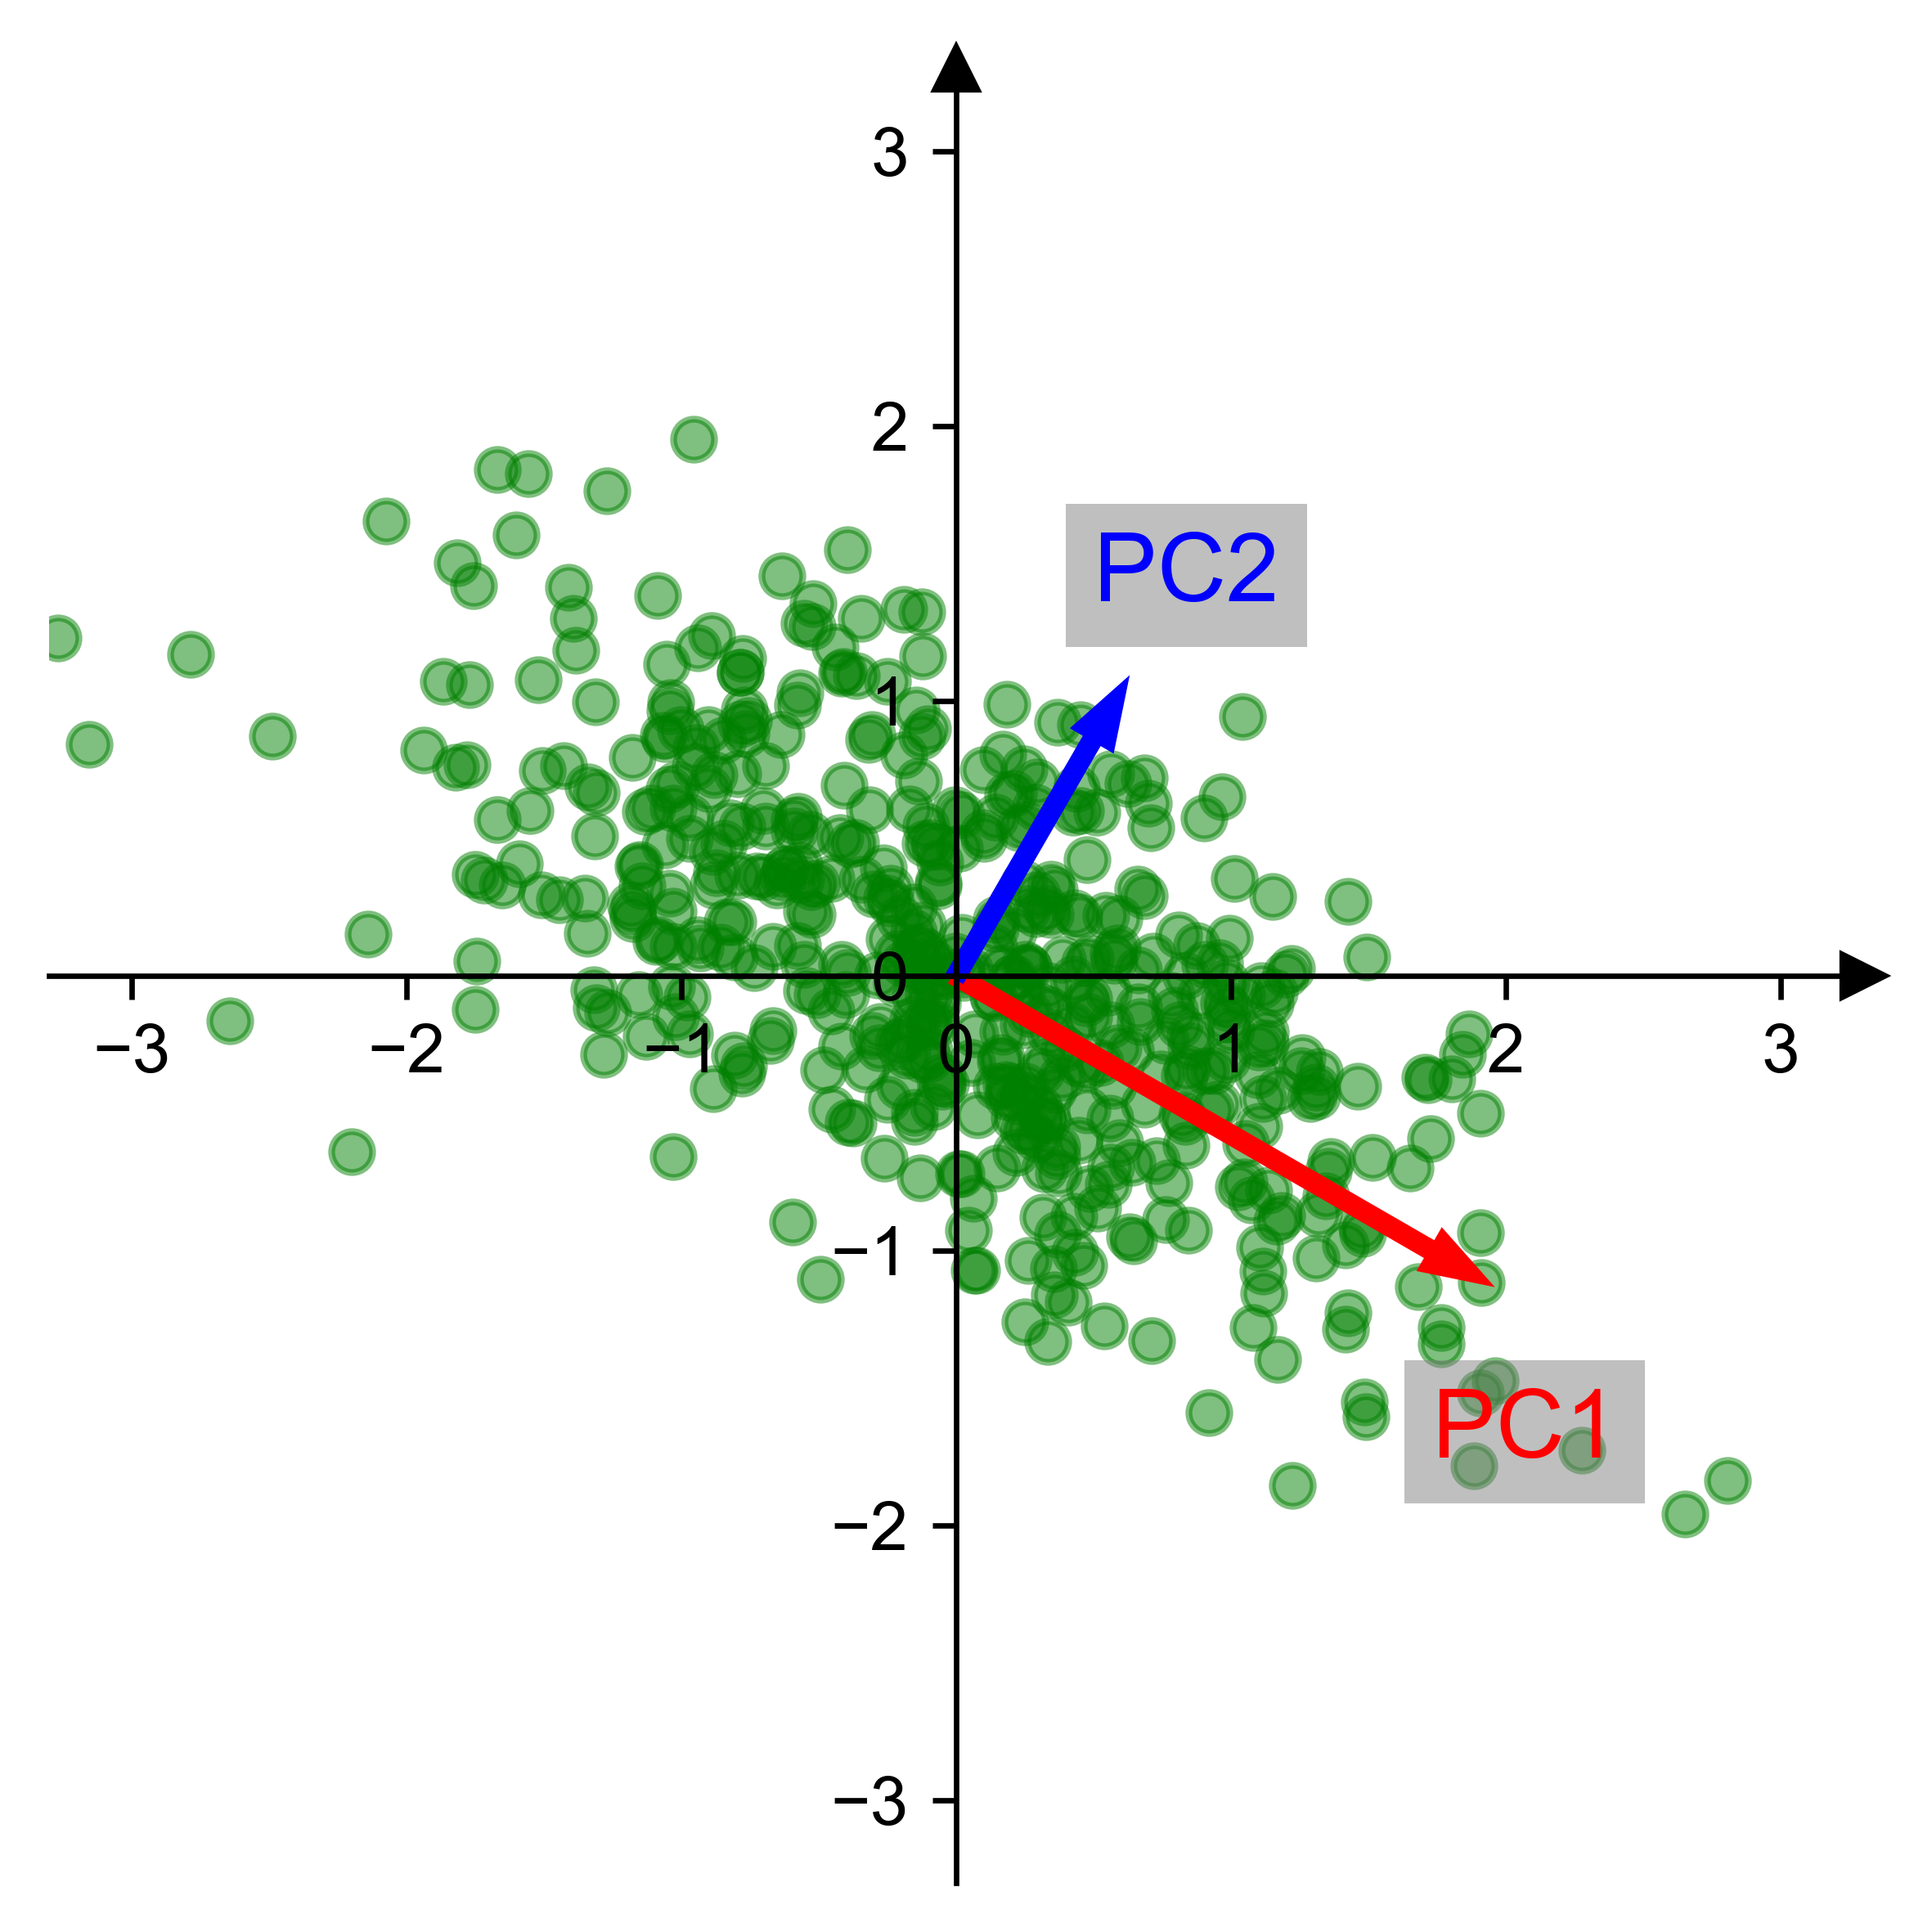
\includegraphics{graphics/PCA_first_demo.png}\\
The two \textit{principal axes/directions} (PCs) found by Principal Component Analysis for a set of data (green). The longer, red (shorter, blue) arrow represents the direction of largest (smallest) variance. The data points can be seen to spread more (less) along that direction. \par
Now the problem is to find, under what situation $\textbf{e}^T Q \textbf{e}$ will assume its largest value. Here, we introduce a famous technique, called \index{Lagrange Multiplier}\keywordhl{Lagrange Multiplier}, coming from elementary Calculus. We will proceed with the case of two variables for brevity.
\begin{thm}[Lagrange Multiplier]
\label{thm:LagrangeMul}
To find the extremal values attained by a function $f(u,v,\cdots)$, under the constraint $g(u,v,\cdots) = 0$, we consider the expression
\begin{align*}
h(u,v,\cdots) = f(u,v,\cdots) - \lambda g(u,v,\cdots)
\end{align*}
where $\lambda$ is a constant so that the system below has a solution:
\begin{align*}
\begin{cases}
\partial h/\partial u &= 0 \\
\partial h/\partial v &= 0 \\
\vdots &= 0
\end{cases}
\end{align*}
$\partial/\partial u$ ($\partial/\partial v$) means differentiating with respect to $u$ ($v$) only while treating other variables as constants. The values of $u$ and $v$ (as well as other variables) required to attain the extremums for $f$ are determined by solving the system of equations above. 
\end{thm}
We are now going to find the value of $x'$ and $y'$ so that $\textbf{e}^T Q \textbf{e}$ obtains the maximum for $\textbf{e}^T = (x',y')$. The constraint is that $\textbf{e}$ is a unit vector as a direction, and hence by the method of Lagrange Multiplier outlined above, we have
\begin{align*}
g(x',y') = x'^2 + y'^2 - 1 = 0
\end{align*}
and with $f(x',y') = \textbf{e}^T Q \textbf{e}$
\begin{align*}
h(x',y') &= (\textbf{e}^T Q \textbf{e}) - \lambda(x'^2 + y'^2 - 1) \\
&= \begin{bmatrix}
x' & y' \\
\end{bmatrix}
\begin{bmatrix}
\text{Cov}(X, X) & \text{Cov}(X, Y) \\
\text{Cov}(Y, X) & \text{Cov}(Y, Y) 
\end{bmatrix}
\begin{bmatrix}
x' \\
y'
\end{bmatrix}
- \lambda(x'^2 + y'^2 - 1) \\
&= x'^2 \text{Cov}(X, X) + 2x'y' \text{Cov}(X, Y) + y'^2\text{Cov}(Y, Y) - \lambda(x'^2 + y'^2 - 1)
\end{align*}
according to Properties \ref{proper:variancemul}. Carrying out the differentiation gives
\begin{align*}
\begin{cases}
\partial h/\partial x' &= 2x'\text{Cov}(X, X) + 2y'\text{Cov}(X, Y) - 2\lambda x' = 0 \\
\partial h/\partial y' &= 2x'\text{Cov}(X, Y) + 2y'\text{Cov}(Y, Y) - 2\lambda y' = 0
\end{cases}    
\end{align*}
This system can be immediately be simplified and recognised as
\begin{align*}
2 \begin{bmatrix}
\text{Cov}(X, X)-\lambda & \text{Cov}(X, Y) \\
\text{Cov}(Y, X) & \text{Cov}(Y, Y)-\lambda
\end{bmatrix}
\begin{bmatrix}
x' \\
y'
\end{bmatrix} &= 0\\
(Q-\lambda I)\textbf{e} &= 0
\end{align*}
which is an eigenvalue problem as introduced in Section \ref{section:eigensection}. Hence we conclude that $f(x',y') = \textbf{e}^T Q \textbf{e}$ can attain an extremal value when $\textbf{e}^T = (x',y')^T$ is a unit eigenvector of $Q$. Notice that since $Q$ is a symmetric matrix, the eigenvectors of $Q$ form an orthonormal basis and are orthogonal to each other by Properties \ref{proper:orthobasissym}. The corresponding magnitude of variance ${\textbf{e}^{(j)}T} Q \textbf{e}^{(j)}$ for the $j$-th eigenvector is
\begin{align*}
{\textbf{e}^{(j)}T} (Q \textbf{e}^{(j)}) &= {\textbf{e}^{(j)}T} (\lambda_j \textbf{e}^{(j)}) \\
&= \lambda_j ({\textbf{e}^{(j)}T} \textbf{e}^{(j)}) \\
&= \lambda_j \norm{\textbf{e}^{(j)}} \\
&= \lambda_j 
\end{align*}
where we have used the facts that $Q \textbf{e}^{(j)} = \lambda_j \textbf{e}^{(j)}$ as per Definition \ref{defn:eigen} and the length of a unit vector is $1$. This means that the variance along the direction of eigenvector is exactly equal to the corresponding eigenvalue. Note that orthogonal diagonalization (see the discussion below Definition \ref{defn:coordtransquad}) transforms the quadratic form to a diagonal matrix consisted of the eigenvalues $\lambda_j$, with respect to the coordinate system made up of the orthonormal eigenvectors $\textbf{e}^{(j)}$. Therefore, from this perspective we can come to the same conclusion that the variance of a transformed variable along the direction indicated by each eigenvector is equal to its eigenvalue, and further, the covariance between two orthogonal directions represented by any pair of distinct eigenvectors are zero, and hence the transformed variables are made uncorrelated. 
\begin{thm}[Principal Component Analysis]
For a covariance matrix $Q$ (which happens to be symmetric), the variance $\textbf{e}^T Q \textbf{e}$ achieves its maximum value $\lambda_1$ along the direction $\textbf{e}^{(1)}$, the largest eigenvalue of $Q$ and the associated unit eigenvector. Generalizing, as $Q$ has $n$ orthonormal eigenvectors $\textbf{e}^{(1)}, \textbf{e}^{(2)}, \cdots, \textbf{e}^{(n)}$, arranged by the magnitude of corresponding eigenvalues $\lambda_1 > \lambda_2 > \cdots > \lambda_n$ from largest to smallest, the largest variance will be $\lambda_1$ when the direction is along $\textbf{e}^{(1)}$, the second largest will be $\lambda_2$ for $\textbf{e}^{(2)}$ and so on, with the smallest variance being $\lambda_n$ for $\textbf{e}^{(n)}$. This set of orthonormal eigenvectors are called the \index{Principal Axes}\index{Principal Directions}\keywordhl{principal axes/directions} in Principal Component Analysis.
\end{thm}
As a side note, any quadratic form $\textbf{e}^TB\textbf{e}$ will attain its maximum and minimum when $\textbf{e}$ is the eigenvector that represents the largest and smallest eigenvalue, which will also be the value that $\textbf{e}^TB\textbf{e}$ takes when it happens. As before, this is under the constraint that $\textbf{e}$ is a unit vector, and this result bears the name of \textit{Constrained Extremum Theorem}.\par
Going back to the problem of Principal Component Analysis, for each principal direction $\textbf{e}^{(j)}$ and the variance $\lambda_{j}$, we can compute the ratio of \index{Explained Variance}\keywordhl{explained variance}, which is the fraction of  $\lambda_{j}$ over the total variance, the sum of eigenvalues/variances from all eigenvectors for the covariance matrix. This quantity allows us to access how well the principal direction contributes to the total variance. In the coordinate system constructed by the orthonormal eigenvectors of $Q$, $[\textbf{e}] = [\textbf{e}^{(1)}|\textbf{e}^{(2)}|\cdots|\textbf{e}^{(n)}]$, the new coordinates for any data point are $\vec{u}_i = [\textbf{e}]^T \vec{x}_i$ (see Section \ref{section:orthogeometricsub}). By the Spectral Theorem \ref{thm:spectral}, this $\vec{u}_i$ can be regarded to be the projection of $\vec{x_i}^T = (x_i, y_i)^T$, the $i$-th pair of data, onto the principal directions and are called the \index{Principal Components}\keywordhl{principal components (PCs)}. \par
Usually, at the start of PCA we will detrend the data and remove the mean from each variable, such that $x'_i = x_i - \bar{x}$ and $y'_i = y_i - \bar{y}$ are used to replace $x_i$ and $y_i$. This enables us to express the covariance matrix as $Q = \frac{1}{n}[X'|Y']^T[X'|Y']$ following the end remark of Properties \ref{proper:variancemul}. 
\begin{exmp}
\label{exmp:tempPCA}
The temperature data of two cities $M$ and $N$ are as follows.
\begin{center}
\begin{tabular}{|c|c|c|c|c|c|}
\hline
(in \si{\degree C}) & $M$ & $N$ & & $M$ & $N$ \\
\hline
1st Day & 21.6 & 22.3 & 8th Day & 22.1 & 22.4 \\
\hline
2nd Day & 21.8 & 21.6 & 9th Day & 21.5 & 21.7 \\
\hline
3nd Day & 20.9 & 21.2 & 10th Day & 22.8 & 22.5 \\
\hline
4th Day & 21.6 & 21.7 & 11th Day & 22.2 & 21.6 \\
\hline
5th Day & 23.4 & 23.2 & 12th Day & 23.0 & 23.3 \\
\hline 
6th Day & 24.7 & 24.1 & 13th Day & 24.2 & 24.7 \\
\hline 
7th Day & 22.0 & 23.9 & 14th Day & 23.8 & 23.1 \\
\hline
\end{tabular}
\end{center}
Perform Principal Component Analysis over them and find the most important principal direction, and extract the time-series of the corresponding PC.
\end{exmp}
\begin{solution}
The means of $M$ and $N$ are $\SI{22.5}{\degree C}$ and $\SI{22.6}{\degree C}$ respectively. After detrending by subtracting the respective means, the new data are
\begin{center}
\begin{tabular}{|c|c|c|c|c|c|}
\hline
(in \si{\degree C}) & $M'$ & $N'$ & & $M'$ & $N'$ \\
\hline
1st Day & -1.5 & -0.3 & 8th Day & -0.4 & -0.2 \\
\hline
2nd Day & -0.7 & -1.0 & 9th Day & -1.0 & -0.9 \\
\hline
3nd Day & -1.6 & -1.4 & 10th Day & 0.3 & -0.1 \\
\hline
4th Day & -0.9 & -0.9 & 11th Day & -0.3 & -1.0 \\
\hline
5th Day & 0.9 & 0.6 & 12th Day & 0.5 & 0.7 \\
\hline 
6th Day & 2.2 & 1.5 & 13th Day & 1.7 & 2.1 \\
\hline 
7th Day & -0.5 & 0.4 & 14th Day & 1.3 & 0.5 \\
\hline
\end{tabular}
\end{center}
From Properties \ref{proper:variancemul}, the sample covariance matrix is
\begin{align*}
Q &= 
\frac{1}{14-1}
\begin{bmatrix}
M' \cdot M' & M' \cdot N' \\
N' \cdot M' & N' \cdot N' 
\end{bmatrix} \\
&= \frac{1}{13}
\begin{bmatrix}
-1.5 & -0.7 & -1.6 & \cdots \\
-0.3 & -1.0 & -1.4 
\end{bmatrix}
\begin{bmatrix}
-1.5 & -0.3 \\
-0.7 & -1.0 \\
-1.6 & -1.4 \\
\vdots
\end{bmatrix} \\
&= \frac{1}{13}
\begin{bmatrix}
18.18 & 13.66 \\
13.66 & 13.64
\end{bmatrix} = 
\begin{bmatrix}
1.398 & 1.051 \\
1.051 & 1.049
\end{bmatrix}
\end{align*}
The unit eigenvectors for $Q$ and thus the principal directions can be found to be $\textbf{e}^{(1)} = (0.763, 0.647)^T$ with a larger variance $\lambda_1 = \SI{2.289}{\square {(\degree C)}}$, and $\textbf{e}^{(2)} = (-0.647, 0.763)^T$ of a smaller variance $\lambda_2 = \SI{0.159}{\square {(\degree C)}}$. The first principal component accounts for $\frac{2.289}{2.289+0.159} \approx 93.5\%$ of the total variance.\\
\\
We can project every pair of data $\vec{x}'^T_i = (m'_i, n'_i)^T$ onto the principal directions by computing $\vec{u}_i = [\textbf{e}]^T\vec{x}'_i$, where $[\textbf{e}] = [\textbf{e}^{(1)}|\textbf{e}^{(2)}]$. The resulting principal components time-series are 
\begin{center}
\begin{tabular}{|c|c|c|c|c|c|c|c|}
\hline
 & D-1 & D-2 & D-3 & D-4 & D-5 & D-6 & D-7 \\
\hline
$u^{(1)}$ & -1.338 & -1.181 & -2.126 & -1.268 & 1.075 & 2.648 & -0.123 \\
\hline
$u^{(2)}$ & 0.741 & -0.310 & -0.034 & -0.105 & -0.124 & -0.278 & 0.628 \\
\hline
 & D-8 & D-9 & D-10 & D-11 & D-12 & D-13 & D-14 \\
\hline
$u^{(1)}$ & -0.434 & -1.345 & 0.164 & -0.875 & 0.834 & 2.655 & 1.315 \\
\hline
$u^{(2)}$ & 0.106 & -0.040 & -0.270 & -0.569 & 0.211 & 0.503 & -0.459 \\
\hline
\end{tabular}
\end{center}
In details, the two principal components for the first day is computed by
\begin{align*}
\begin{bmatrix}
u_1^{(1)} \\
u_1^{(2)} 
\end{bmatrix}
=
\begin{bmatrix}
0.763 & 0.647 \\
-0.647 & 0.763
\end{bmatrix}
\begin{bmatrix}
-1.5 \\
-0.3
\end{bmatrix}
=
\begin{bmatrix}
-1.338\\
0.741
\end{bmatrix}
\end{align*}
The original (detrended) data can be recovered by $\vec{x}'_i = [\textbf{e}]\vec{u}'_i$. If we want to extract the signal originated from the first principal direction only, we can simply remove other column eigenvector(s) in $[\textbf{e}]$ as well as discard the other principal value(s) in $\vec{u}'_i$. The time-series reconstructed by the first PC mode is hence computed by $\vec{x}'_i = \textbf{e}^{(1)}u_i^{(1)}$:
\begin{center}
\begin{tabular}{|c|c|c|c|c|c|c|c|}
\hline
(in \si{\degree C}) & D-1 & D-2 & D-3 & D-4 & D-5 & D-6 & D-7 \\
\hline
M' & -1.021 & -0.901 & -1.622 & -0.968 & 0.820 & 2.020 & -0.094 \\
\hline
N' & -0.865 & -0.763 & -1.374 & -0.820 & 0.695 & 1.712 & -0.079 \\
\hline
 & D-8 & D-9 & D-10 & D-11 & D-12 & D-13 & D-14 \\
\hline
M' & -0.331 & -1.026 & 0.125 & -0.668 & 0.636 & 2.025 & 1.003 \\
\hline
N' & -0.281 & -0.869 & 0.106 & -0.566 & 0.539 & 1.716 & 0.850 \\
\hline
\end{tabular}
\end{center}
For example, for the third day PC1 contributes
\begin{align*}
\vec{x}'_3 =
\begin{bmatrix}
m'_3 \\
n'_3
\end{bmatrix}
=
\textbf{e}^{(1)}u_3^{(1)}
=
\begin{bmatrix}
0.763 \\
0.647
\end{bmatrix}
\begin{bmatrix}
-2.126
\end{bmatrix}
=
\begin{bmatrix}
-1.622 \\
-1.374  
\end{bmatrix}
\end{align*}
\begin{center}
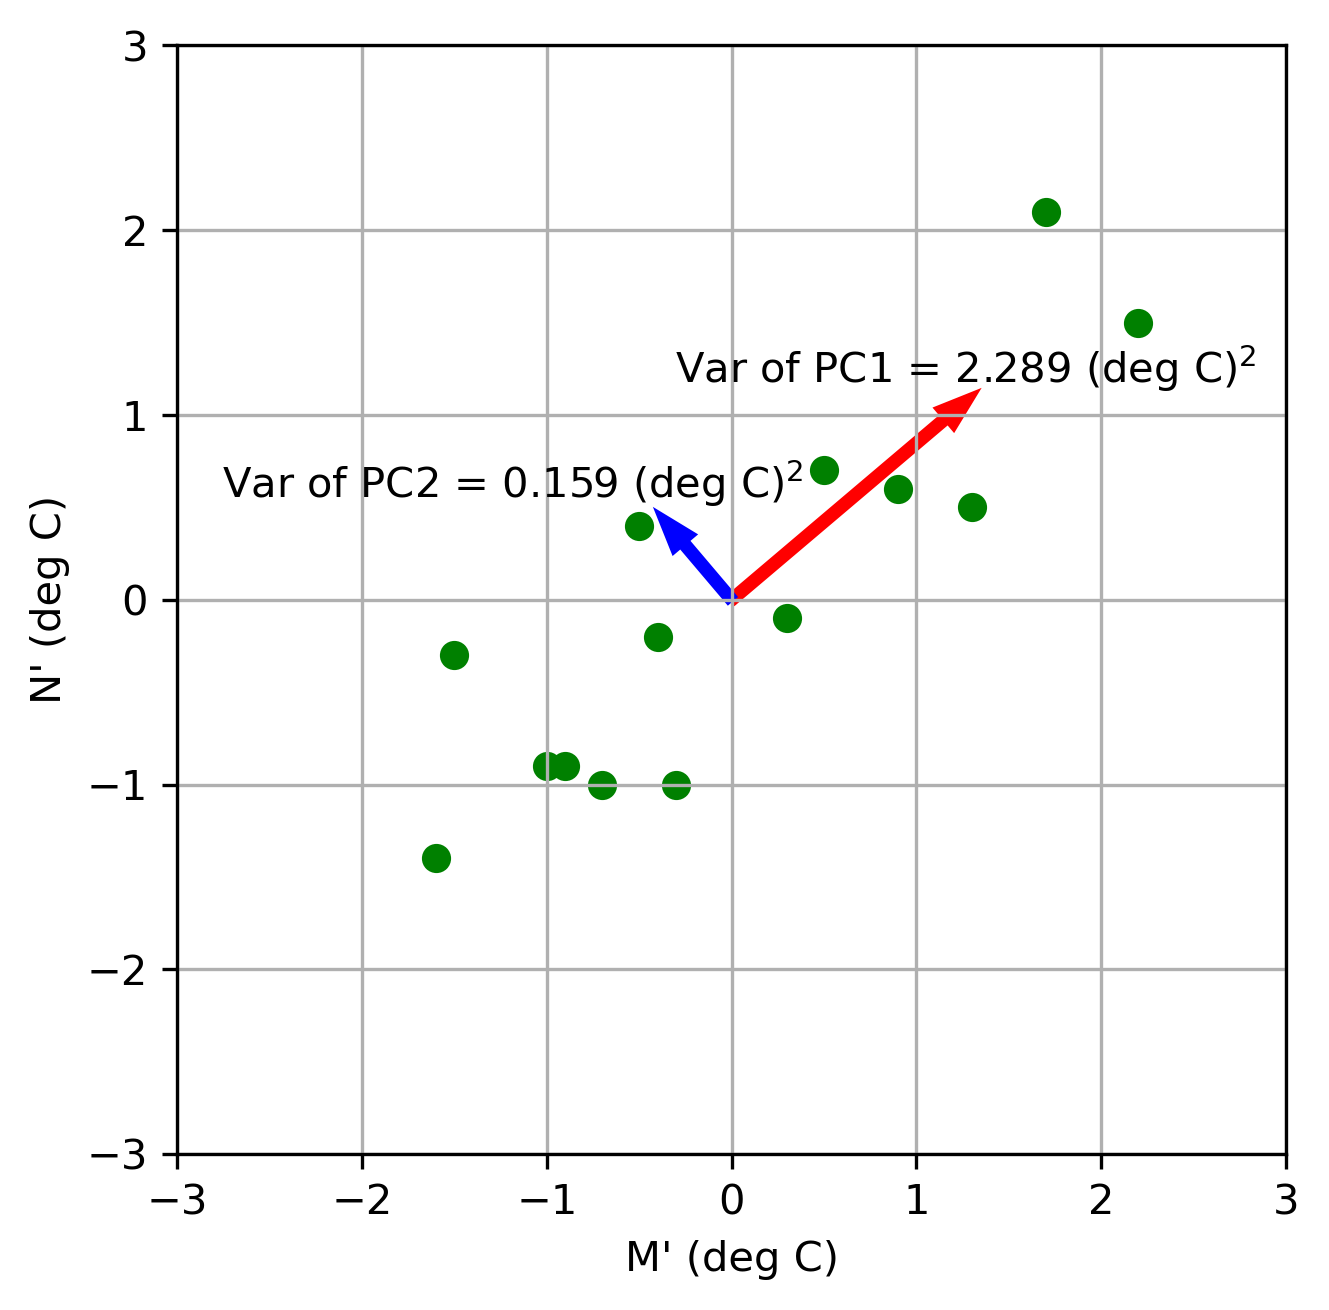
\includegraphics[scale = 0.75]{graphics/PCA_exmp_1.png}\\
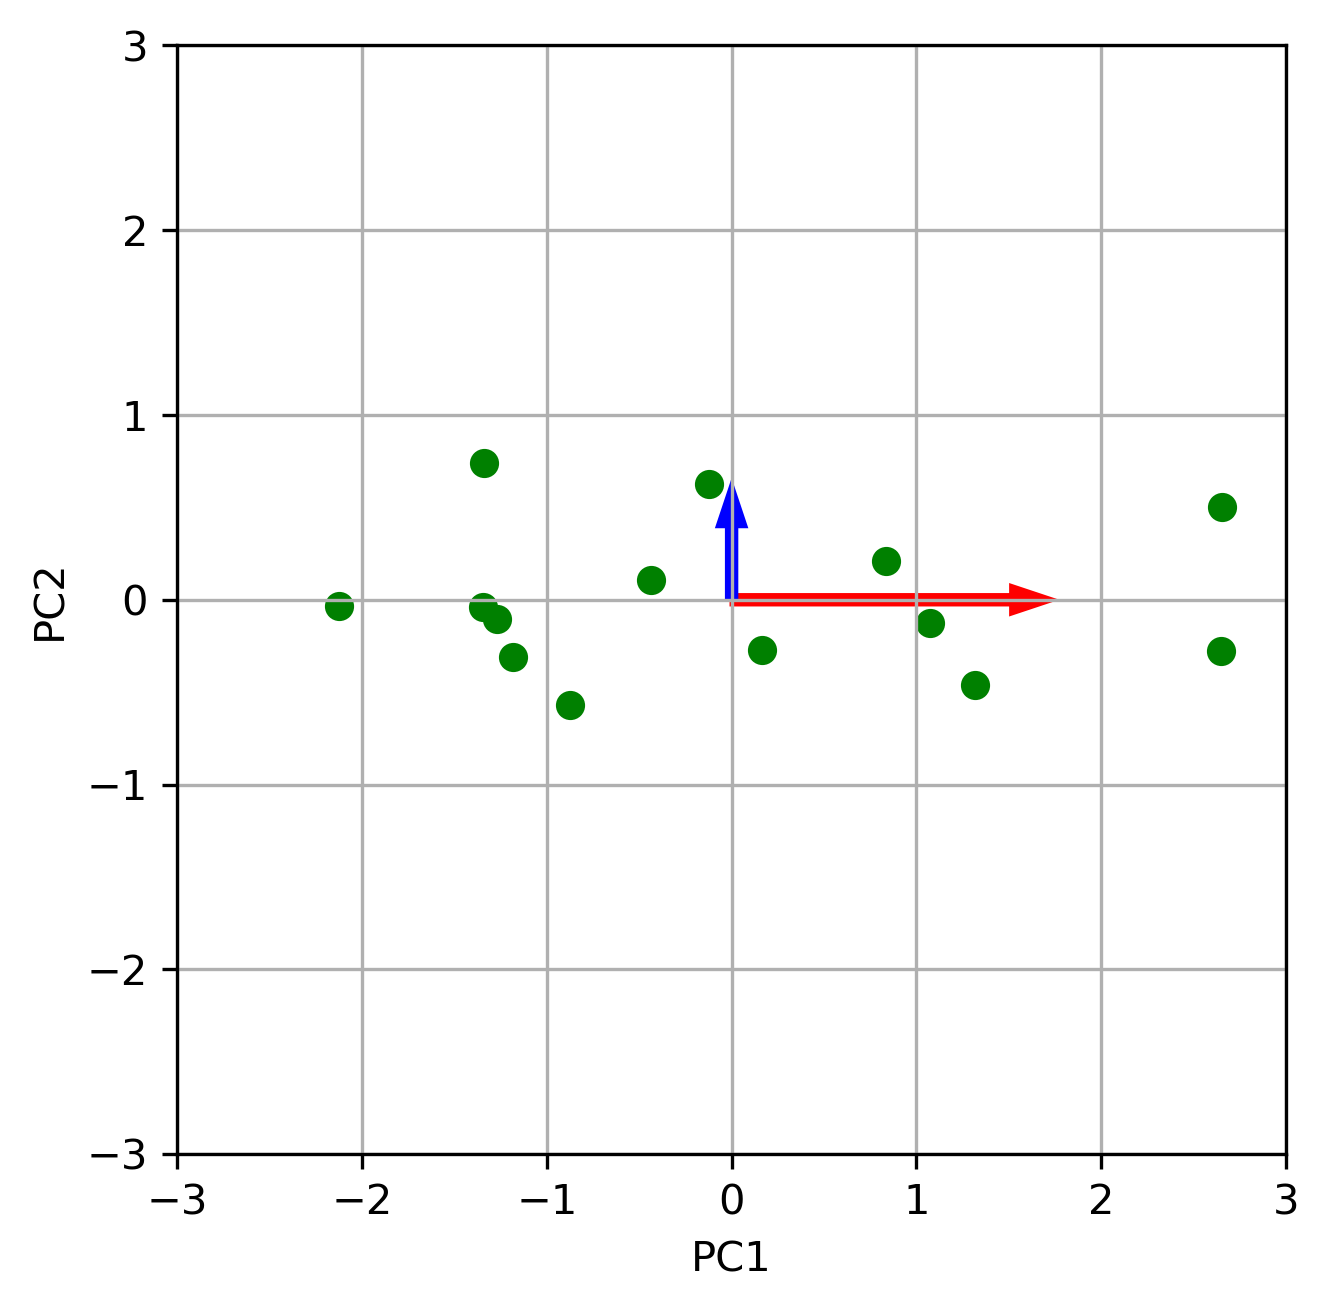
\includegraphics[scale = 0.75]{graphics/PCA_exmp_2.png}\\
The data (green) before and after rotation to the principal axes, with the one with a larger/smaller variance shown as a red/blue arrow.
\end{center}
\begin{center}
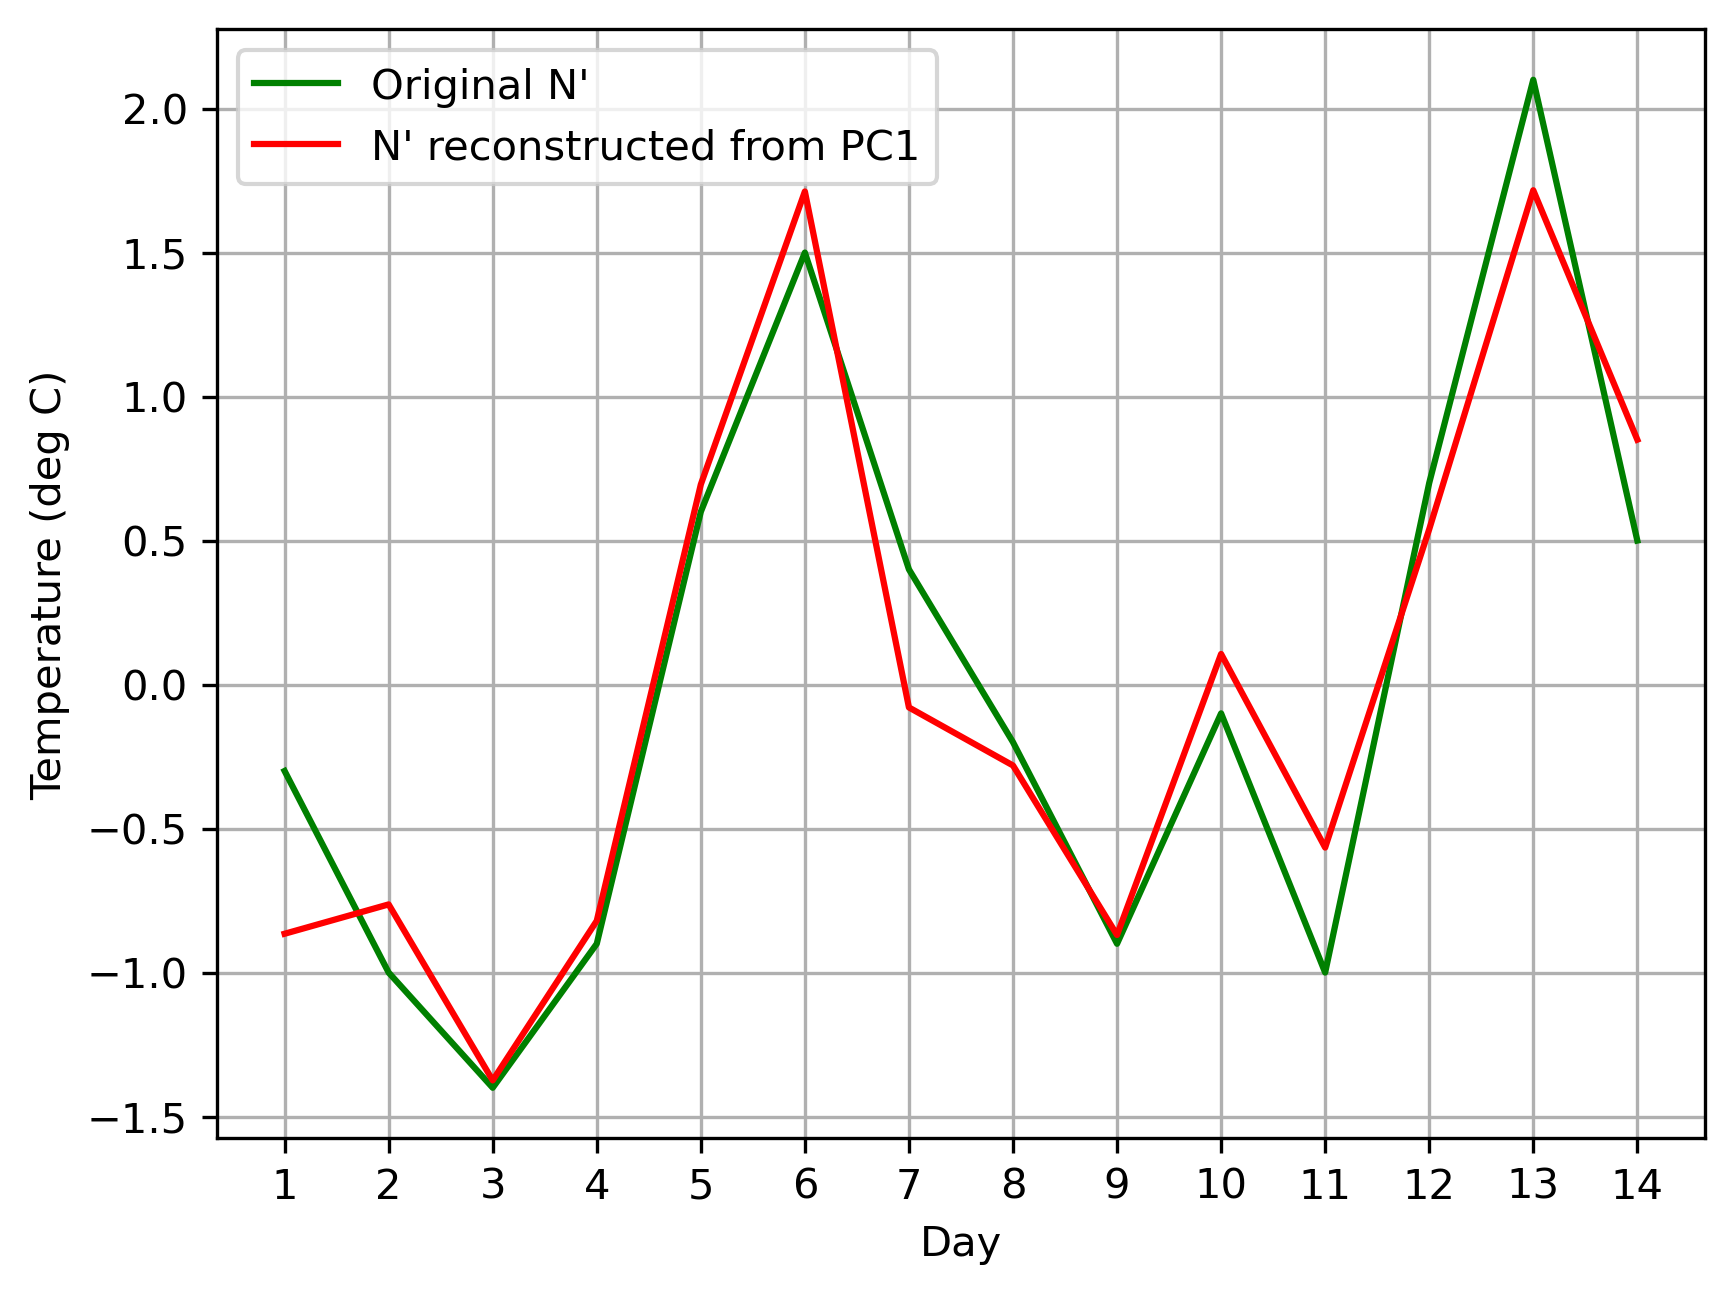
\includegraphics[scale = 0.8]{graphics/PCA_exmp_3.png}\\
Comparison between the original time-series and the one reconstructed using only first PC for $N'$.
\end{center}
\end{solution}

\section{Python Programming}
Since doing EOFs as an Earth Science application is essentially a PCA which has to rely on a computer when the dataset is huge, we will get into the Python programming part first in this chapter. We will need the scikit-learn package (\texttt{sklearn}) for this, and let's use Example \ref{exmp:tempPCA} for demonstration.
\begin{lstlisting}
import numpy as np
from sklearn.decomposition import PCA    

X = np.array([[21.0, 22.3],
              [21.8, 21.6],
              [20.9, 21.2],
              [21.6, 21.7],
              [23.4, 23.2],
              [24.7, 24.1],
              [22.0, 23.0],
              [22.1, 22.4],
              [21.5, 21.7],
              [22.8, 22.5],
              [22.2, 21.6],
              [23.0, 23.3],
              [24.2, 24.7],
              [23.8, 23.1]])
\end{lstlisting}
We have to prepare the data where each column represents the time-series of one variable so the shape of \verb|X| is $(\text{Number of samples}, \text{Number of features})$. Now define a \verb|PCA| object and fit it with the data. We can choose how many PCs to be used, and for now we will keep all of them so that \verb|n_components| $=2$.
\begin{lstlisting}
pca = PCA(n_components=2)
pca.fit(X)    
\end{lstlisting}
We can retrieve the principal directions and variances by
\begin{lstlisting}
print(pca.components_)
print(pca.explained_variance_)    
\end{lstlisting}
which gives
\begin{lstlisting}
[[ 0.76286648  0.64655605]
 [-0.64655605  0.76286648]]
[2.28902525 0.15866706] 
\end{lstlisting}
Notice that the principal directions are arranged in rows so that to get the first one we write \verb|pca.components_[0,:]| that returns \verb|[0.763 0.647]|. The percentage of explained variances are simply computed by
\begin{lstlisting}
print(pca.explained_variance_/np.sum(pca.explained_variance_))
\end{lstlisting}
that returns \verb|[0.9352 0.0648]|. To obtain the time-series of transformed PCs, we simply use the \verb|transform| method:
\begin{lstlisting}
Z = pca.transform(X)
print(Z)
\end{lstlisting}
yielding the expected output of
\begin{lstlisting}
[[-1.33826654  0.74097414]
 [-1.18056259 -0.31027725]
 [-2.12576485 -0.03352339]
 ...
 [ 1.31500445 -0.45908963]]    
\end{lstlisting}
To reconstruct the time-series using only some (the first) PC, we can do the followings.
\begin{lstlisting}
Z_trimmed = np.copy(Z)
Z_trimmed[:,1:] = 0
X_inv = pca.inverse_transform(Z_trimmed)
print(X_inv)
\end{lstlisting}
These generate
\begin{lstlisting}
[[21.47908131 21.73473567]
 [21.59938837 21.83670011]
 [20.87832525 21.22557387]
 ...
 [23.50317282 23.45022409]]    
\end{lstlisting}
equivalent to the last table in Example \ref{exmp:tempPCA} but with the original means included. The following code segments produce the main part of the three plots shown in the example.
\begin{lstlisting}
Y = X - np.mean(X, axis=0)
lambda_1 = pca.explained_variance_[0]
lambda_2 = pca.explained_variance_[1]

plt.scatter(Y[:,0], Y[:,1], color="g")
plt.xlim([-3,3])
plt.ylim([-3,3])
plt.arrow(0,0,lambda_1**0.5*pca.components_[0,0],lambda_1**0.5*pca.components_[0,1], color="r", width=0.05)
plt.arrow(0,0,lambda_2**0.5*pca.components_[1,0],lambda_2**0.5*pca.components_[1,1], color="b", width=0.05)
plt.grid()
plt.gca().set_aspect("equal")
plt.show()

plt.scatter(Z[:,0], Z[:,1], color="g")
plt.xlim([-3,3])
plt.ylim([-3,3])
plt.xlabel("PC1")
plt.ylabel("PC2")
plt.grid()
plt.gca().set_aspect("equal")
plt.show()

plt.plot(np.arange(1,14+1), Y[:,1], color="g", label="Original N'")
plt.plot(np.arange(1,14+1), X_inv[:,1] - np.mean(X, axis=0)[1], color="r", label="N' reconstructed from PC1")
plt.legend()
plt.xticks(np.arange(1,14+1))
plt.show()
\end{lstlisting}

\section{Earth Science Applications: Empirical Orthogonal Functions (EOFs)}
\label{section:EOF}

Here we will read the ERA5 dataset for sea surface temperature (SST) and find the dominant patterns of global SST variability. The data can be retrieved from \href{https://cds.climate.copernicus.eu/datasets/reanalysis-era5-single-levels?tab=download}{https://cds.climate.copernicus.eu/datasets/reanalysis-era5-single-levels?tab=download} and selecting the options "Type: Reanalysis, Variable: Sea surface temperature, Time: 00:00, Data format: NetCDF4". We will choose the time period from 1991 to 2020, every month/day, and a spatial domain from \SI{45}{\degree N} to \SI{45}{\degree S} and \SI{110}{\degree E} to \SI{80}{\degree W}. We will also need the land-sea mask that can be downloaded via \href{https://confluence.ecmwf.int/download/attachments/140385202/lsm_1279l4_0.1x0.1.grb_v4_unpack.nc?version=1&modificationDate=1591983422208&api=v2}{https://confluence.ecmwf.int/download/attachments/\\140385202/lsm\_1279l4\_0.1x0.1.grb\_v4\_unpack.nc?version=1\&modificationDate\\=1591983422208\&api=v2}. Now, import the required packages.
\begin{lstlisting}
import matplotlib.pyplot as plt
import numpy as np
import pandas as pd
import xarray as xr
from sklearn.decomposition import PCA
import cartopy.crs as ccrs
\end{lstlisting}
Load the SST data, work on coarse grids with a $\SI{2.5}{\degree} \times \SI{2.5}{\degree}$ spatial resolution (optional to the reduce computational cost), and exclude leap days.
\begin{lstlisting}
SST_nc = xr.open_dataset("ERA5_SST.nc")
coarse_lat = np.array(SST_nc["latitude"][::10]) # 0.25 deg * 10 = 2.5 deg
coarse_lon = np.array(SST_nc["longitude"][::10])
time = pd.Series(SST_nc["valid_time"])
no_leapdays = ~((time.dt.month == 2) & (time.dt.day == 29))
\end{lstlisting}
Also, prepare the land-sea mask to exclude land grid points and flatten it for indexing later.
\begin{lstlisting}
land_sea_mask_nc = xr.open_dataset("lsm_1279l4_0.1x0.1.grb_v4_unpack.nc")
land_sea_mask = np.array(land_sea_mask_nc["lsm"].sel({"latitude": coarse_lat, "longitude": coarse_lon}, method="nearest")[0, ...])
land_sea_mask = np.where(land_sea_mask > 0, 1, 0).astype(bool)
land_sea_mask_flatten = land_sea_mask.flatten()
\end{lstlisting}
Preprocessing the SST data by subtracting the yearly climatology to acquire the anomaly fields, scale them by the square roots of cosines of the latitudes to account for area weighting and keep only the valid overwater grid points using the land-sea mask:
\begin{lstlisting}
SST_data_arr = np.array(SST_nc["sst"].sel({"latitude": coarse_lat, "longitude": coarse_lon}))
SST_data_arr_no_leap = SST_data_arr[no_leapdays, ...].reshape(30,365,len(coarse_lat),len(coarse_lon))
# The SST array now has the shape of 30 years * 365 days * nlat * nlon
SST_clim = np.mean(SST_data_arr_no_leap, axis=0)
SST_anomaly = SST_data_arr_no_leap - SST_clim

cos_factor_root = np.cos(np.deg2rad(coarse_lat))**0.5
SST_anomaly_weighted = SST_anomaly * cos_factor_root[None,None,:,None]

SST_flatten = SST_anomaly_weighted.reshape(30*365, len(coarse_lat)*len(coarse_lon))
SST_valid = SST_flatten[:, ~land_sea_mask_flatten]
\end{lstlisting}
Call the PCA and fit it with the prepared, flattened SST data:
\begin{lstlisting}
SST_PCA = PCA(n_components=3) # any number will be fine
SST_PCA.fit(SST_valid)
\end{lstlisting}
Then, recover the latitude-longitude structure of the first PC:
\begin{lstlisting}
PC1 = np.full(len(coarse_lat)*len(coarse_lon), np.nan)
PC1[~land_sea_mask_flatten] = SST_PCA.components_[0,:] # Fill PC1 at appropriate overwater entries
PC1_2D = PC1.reshape(len(coarse_lat), len(coarse_lon)) / cos_factor_root[:,None] # Invert the cosine factor
\end{lstlisting}
and plot it on the map.
\begin{lstlisting}
plt.figure()
plt.subplot(111, projection=ccrs.PlateCarree(central_longitude=180)) # the central_longitude option is needed to plot across the International Date Line
plt.pcolormesh(coarse_lon, coarse_lat, PC1_2D, cmap="coolwarm", vmin=-0.08, vmax=0.08, transform=ccrs.PlateCarree())
plt.gca().coastlines()
gl = plt.gca().gridlines(draw_labels=True)
gl.top_labels = False
plt.title("First EOF of Sea Surface Temperature (SST) - ENSO")
plt.colorbar(orientation="horizontal", label="Temperature Anomaly (deg C)")
plt.savefig("SST_EOF")
\end{lstlisting}
You should be able to get the following figure.
\begin{center}
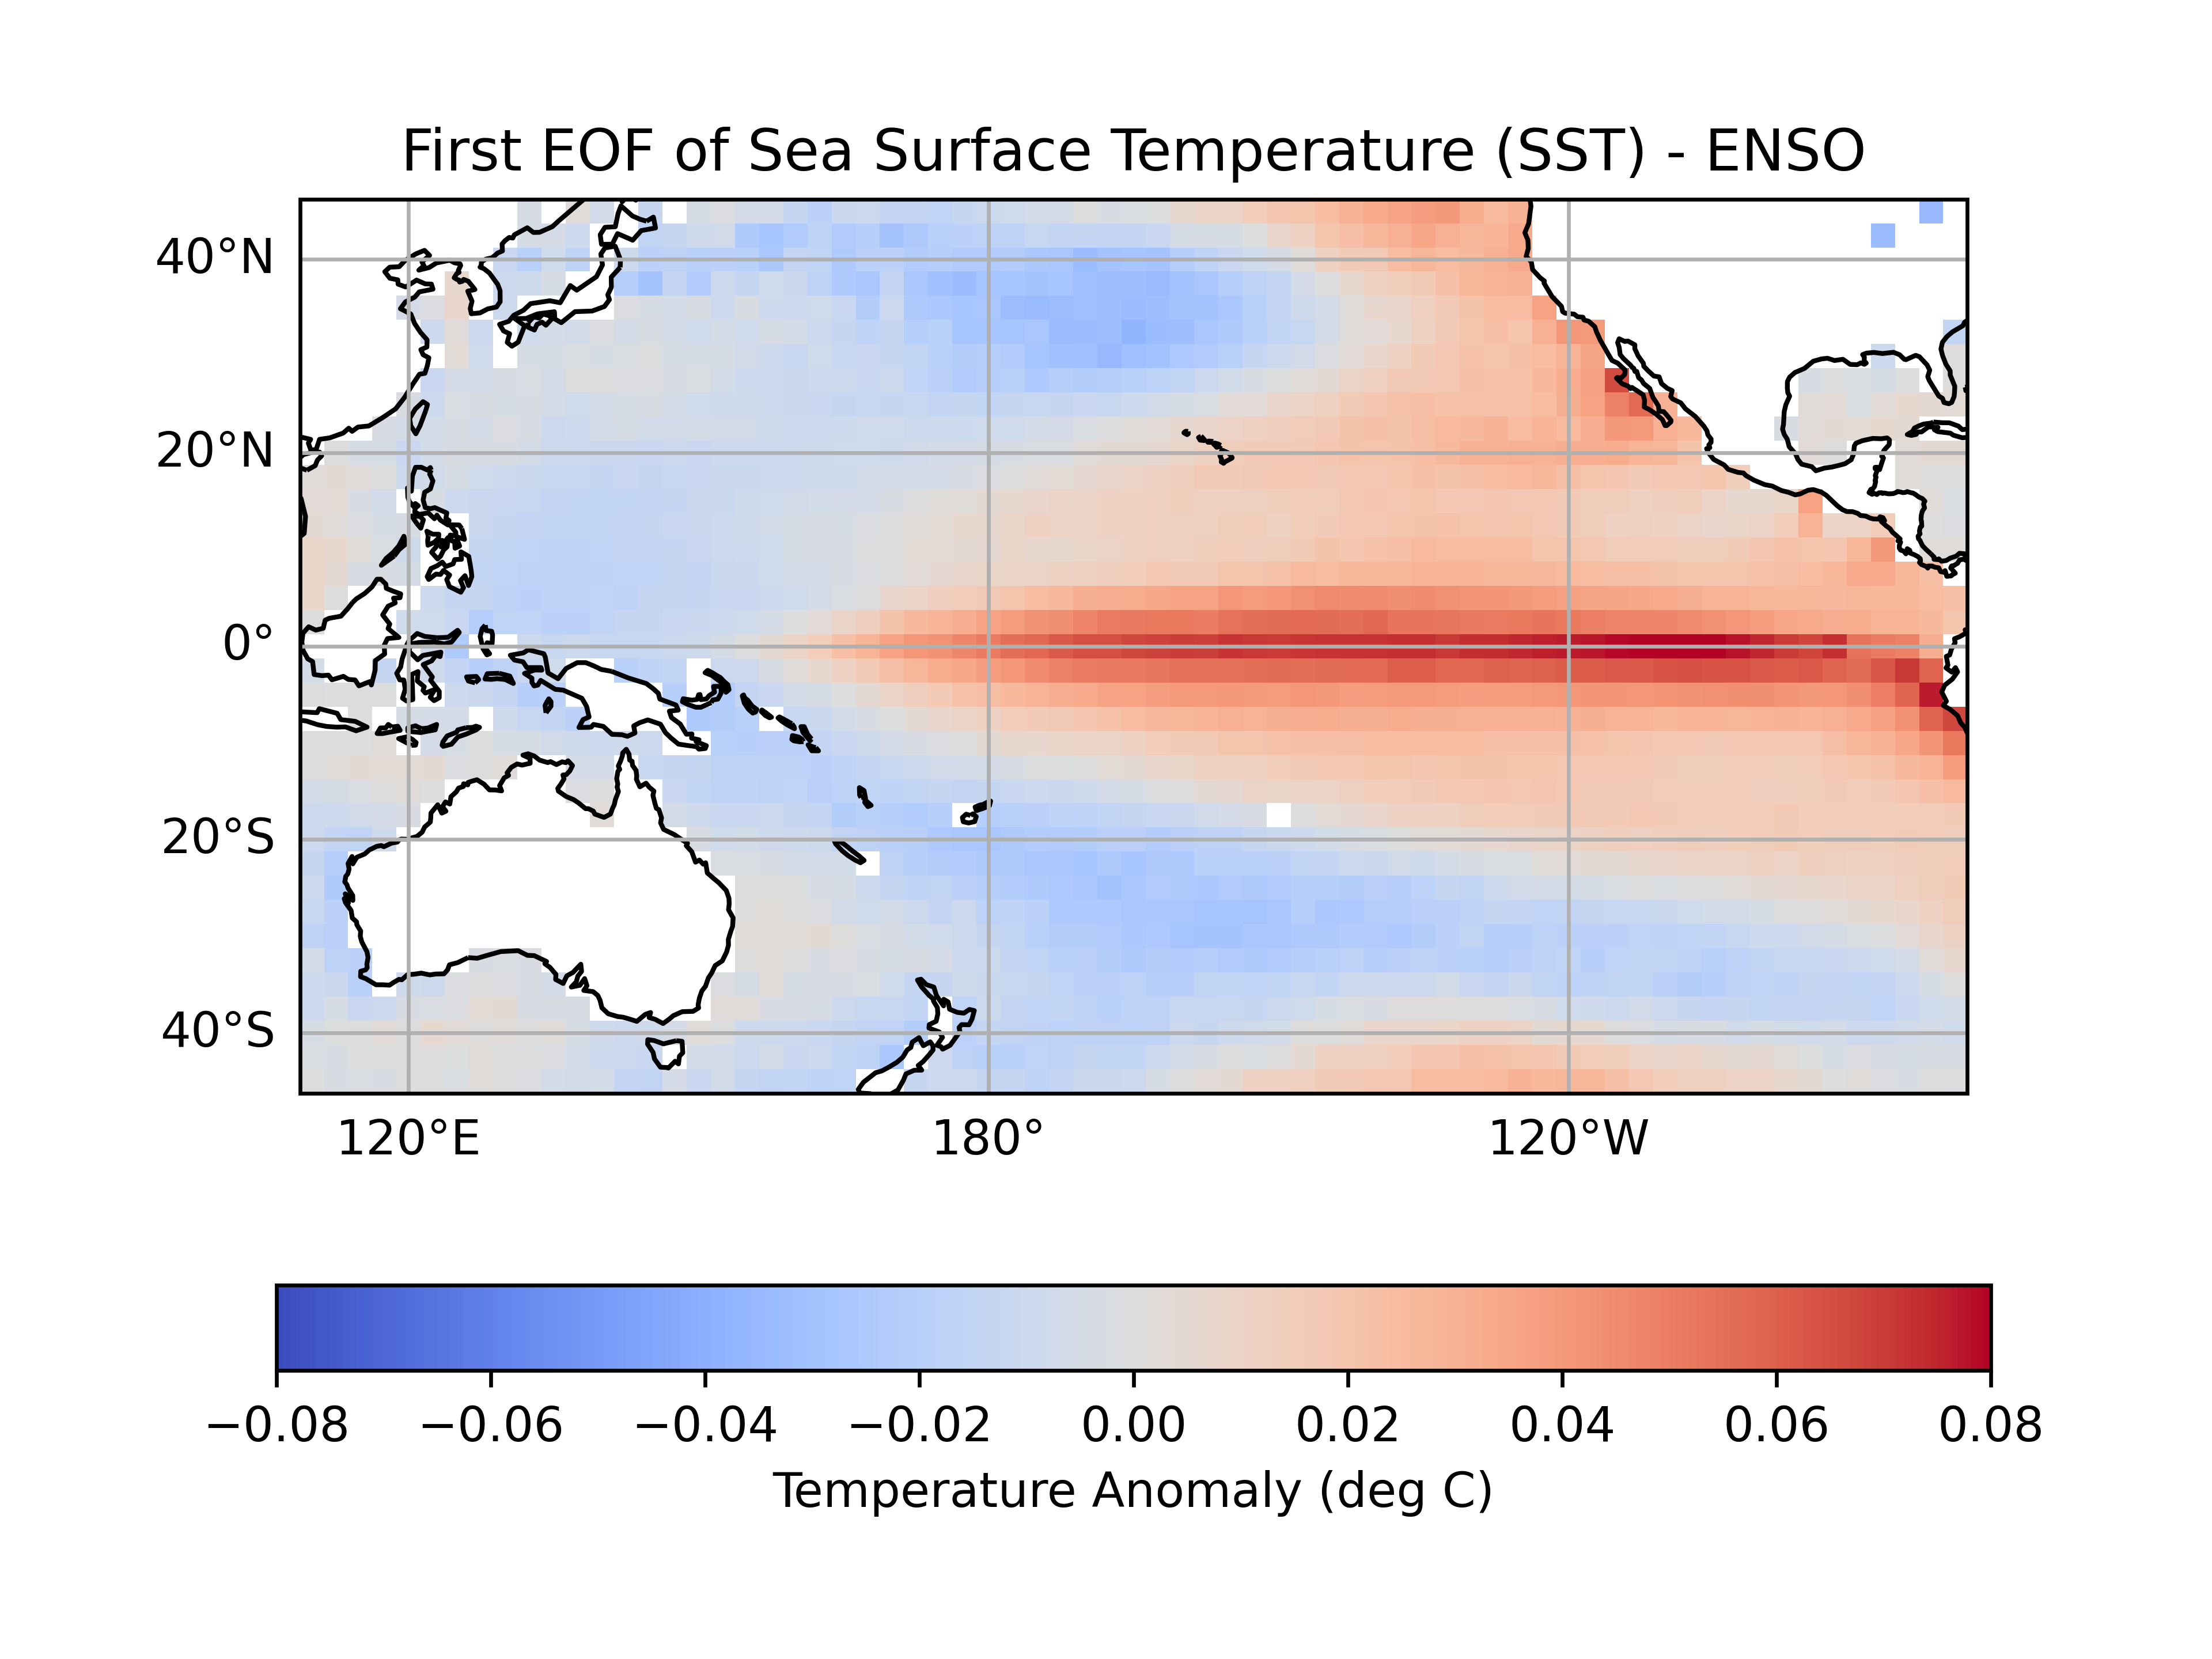
\includegraphics[scale=0.75]{graphics/SST_EOF.png}
\end{center}
This EOF pattern represents the \index{El Niño–Southern Oscillation (ENSO)}\keywordhl{El Niño–Southern Oscillation (ENSO)} phenomenon where the western Pacific gets cooler (warmer) and eastern Pacific becomes warmer (cooler) during the El Niño (La Niña) phase.

\section{Exercises}

\begin{Exercise}
Identify the following conic sections and eliminate the cross-product terms by an appropriate rotation.
\begin{enumerate}[label=(\alph*)]
\item $x^2 + 5xy + 3y^2 = 1$,
\item $x^2 - xy + 2y^2 = 4$,
\item $x^2 + 2xy + y^2 = 1$, what is the graph generated? 
\end{enumerate}
\end{Exercise}

\begin{Exercise}
Find a new expression for the standard hyperbola $y^2 - x^2 = 1$ if a anti-clockwise rotation of $60$ degrees is done. What about a reflection along the $x$-axis?
\end{Exercise}

\begin{Exercise}
Three-dimensional quadrics can also be treated in a similar fashion to two-dimensional conic sections. Find the length of three axes for an ellipsoid $x^2 + y^2 + z^2 + 0.5xy - yz + 0.5xz = 1$ by doing an orthogonal coordinate transformation. What is the requirement for a three-dimensional quadratic form to represent an ellipsoid?
\end{Exercise}

\begin{Exercise}
Use the Sylvester's Law of Inertia to argue that a symmetric matrix $B$ is positive-definite if and only if $B = P^TP$ for some invertible matrix $P$. Hint: Consider $P^T IP$.
\end{Exercise}

\begin{Exercise}
Find the covariance matrix for three pressure time-series over $10$ days at cities $X$, $Y$, $Z$ (in hPa, relative to $1000$ hPa), which take the values
\begin{center}
\begin{tabular}{|c|c|c|}
\hline
$X$ & $Y$ & $Z$ \\
\hline
17.1 & 19.2 & 22.0 \\
\hline
18.5 & 16.9 & 25.4 \\
\hline
14.8 & 15.3 & 17.3 \\
\hline
19.7 & 21.6 & 23.5 \\
\hline
24.1 & 22.3 & 26.8 \\
\hline
21.6 & 20.9 & 23.2 \\
\hline 
28.0 & 26.7 & 29.5 \\
\hline
24.3 & 25.0 & 22.5 \\
\hline
20.3 & 21.5 & 27.2 \\
\hline
23.4 & 22.4 & 24.6 \\
\hline
\end{tabular}
\end{center}
Find the variance of $W = X - 0.5Y - 0.5Z$.
\end{Exercise}

\begin{Exercise}
Carry out Principal Component Analysis on the data set above. Find the Principal Directions and the ratio of explained variance for each of them. Reconstruct the data using the first principal component with largest variance only.
\end{Exercise}

\begin{Exercise}
Download the ERA5 datasets for \SI{200}{hPa} and \SI{850}{hPa} zonal winds, as well as total column water over some $10$ to $20$ years from \SI{15}{\degree N} to \SI{15}{\degree S} and \SI{60}{\degree E} to \SI{160}{\degree E}. Standardize the three variables via dividing them by their standard deviations respectively, concatenate them and follow the procedure outlined in Section \ref{section:EOF} to do the so-called \textit{combined EOFs}. Recover the physical patterns through multiplying the entries of EOF modes back by the standard deviations of corresponding variables. You should be able to observe the appearance of \textit{Madden-Julian Oscillation (MJO)} from the first two EOFs. 
\end{Exercise}


\chapter{Inner Product Spaces}
\label{chap:innerchap}

In Chapter \ref{chap:vec_space}, we have discussed what it means to be a vector space. Previously, it is accompanied by the dot product operation as defined in Section \ref{section:dotprod} that gives rise to the notion of \textit{Euclidean} distance in $\mathbb{R}^n$ (complex dot product for $\mathbb{C}^n$). In this chapter, we will show that the usual dot product is not the only way to measure the distance between vectors: we can equip any vector space with a so-called \textit{inner product} that fulfills certain criteria and leads to an alternative expression for the length of vectors, in place of the dot product. This generalizes a vector space to an \textit{inner product space}, and many concepts for a vector space, like orthogonality, can be adapted to be applied in inner product spaces. Particularly, we will have the \textit{adjoint} as an inner product space equivalent to the usual transpose. Finally, we will talk about \textit{special polynomials} which are generated by considering suitable inner products and are often used in Earth Science applications, such as solving \textit{partial differential equations (PDEs)}.

\section{Definition and Properties of Inner Product Spaces}

\subsection{Requirements of Inner Products}

As introduced in the beginning, an \index{Inner Product Space}\keywordhl{inner product space} is a vector space (either real or complex) that comes with an \index{Inner Product}\keywordhl{inner product} operation that is akin to the usual dot product. To qualify as a valid inner product, it has to fulfill four requirements as suggested below.
\begin{defn}[Inner Product (Space)]
\label{defn:innerprod}
An inner product on a vector space $\mathcal{V}$ over $\mathbb{R}$ ($\mathbb{C}$) is a function that takes a pair of vectors $\vec{u}, \vec{v} \in \mathcal{V}$ as the input and returns an $\mathbb{R}$ ($\mathbb{C}$) scalar, denoted by $\langle \vec{u}, \vec{v} \rangle$. Then, for any $\vec{u}, \vec{v}, \vec{w} \in \mathcal{V}$ and scalar $a \in \mathbb{R}$ ($\mathbb{C}$), the following four axioms have to hold.
\begin{enumerate}
    \item $\langle \vec{u}, \vec{v} \rangle = \langle \vec{v}, \vec{u} \rangle$ ($\langle \vec{u}, \vec{v} \rangle = \overline{\langle \vec{v}, \vec{u} \rangle}$) ((Conjugate) Symmetry);
    \item $\langle \vec{u}+\vec{v}, \vec{w} \rangle = \langle \vec{u}, \vec{w} \rangle + \langle \vec{v}, \vec{w} \rangle$ (Additivity);
    \item $\langle a\vec{u}, \vec{v} \rangle = a\langle \vec{u}, \vec{v} \rangle$ (Homogeneity); and
    \item $\langle \vec{v}, \vec{v} \rangle \geq 0$, and $\langle \vec{v}, \vec{v} \rangle = 0$ if and only if $\vec{v} = \textbf{0}$ is the zero vector. (Positivity)
\end{enumerate}
The second and third condition can be combined into \textit{linearity} (in the first argument): given another scalar $b \in \mathbb{R}$ ($\mathbb{C}$), we have $\langle a\vec{u}+b\vec{v}, \vec{w} \rangle = a\langle \vec{u}, \vec{w} \rangle + b\langle \vec{v}, \vec{w} \rangle$. A real (complex) vector space equipped with an inner product is then known as a real (complex) inner product space. 
\end{defn}
Short Exercise: Show that $\langle a\vec{u}, b\vec{v} \rangle = a\overline{b}\langle \vec{u}, \vec{v} \rangle$ for any complex inner product space.\footnote{$\langle a\vec{u}, b\vec{v} \rangle = a\langle \vec{u}, b\vec{v} \rangle = a\overline{\langle b\vec{v}, \vec{u} \rangle} = a\overline{b\langle \vec{v}, \vec{u} \rangle} = a(\overline{b}) \overline{\langle \vec{v}, \vec{u} \rangle} = a\overline{b}\langle \vec{u}, \vec{v} \rangle$ by the first and third axiom.}\par
For now, we will limit ourselves to finite-dimensional vector/inner product spaces until Section \ref{section:infinner}. It is not hard to verify that the above axioms hold for the usual dot product, so $\mathbb{R}^n$ (as well as $\mathbb{C}^n$) is automatically an inner product space when the (complex) dot product is equipped. In this case, they are known as the \index{Standard Inner Product}\keywordhl{standard inner product} and \index{Euclidean $n$-space}\keywordhl{Euclidean $n$-space}. However, $\mathbb{R}^n$ will be a different inner product space when another inner product is used. It can be shown that all alternative inner products that can applied to $\mathbb{R}^n$ are precisely positive-definite symmetric bilinear forms as the extension of positive-definite quadratic forms introduced in the last chapter. Given any positive-definite symmetric bilinear form $B$, it can be verified that $\langle \vec{u}, \vec{v} \rangle = \vec{u}^TB\vec{v}$ will satisfy the real inner product axioms.\footnote{For (1): $\langle \vec{u}, \vec{v} \rangle = \vec{u}^TB\vec{v} = (\vec{u}^TB\vec{v})^T$ since it is only a scalar, and then $(\vec{u}^TB\vec{v})^T = \vec{v}^TB^T\vec{u} = \vec{v}^TB\vec{u} = \langle \vec{v}, \vec{u} \rangle$ due to Properties \ref{proper:transp} and because $B$ is symmetric. (2) and (3) are obvious. For (4), as $B$ is required to be positive-definite, $\langle \vec{v}, \vec{v} \rangle = \vec{v}^TB\vec{v} > 0$ by Definition \ref{defn:quaddefinite} as long as $\vec{v} \neq \textbf{0}$ and it is apparent that $\langle \vec{v}, \vec{v} \rangle = \textbf{0}B\textbf{0} = 0$ when $\vec{v} = \textbf{0}$.} Below are some other properties of inner products extended from the axioms that can be compared to Properties \ref{proper:dotproper} and \ref{proper:complexdot}.
\begin{proper}
\label{proper:innerprod2}
For vectors $\vec{u}, \vec{v}, \vec{w} \in \mathcal{V}$ and scalar $b \in \mathbb{R}$ ($\mathbb{C}$) in a real (complex) inner product space, we have
\begin{enumerate}
    \item $\langle \vec{u} \pm \vec{v}, \vec{w} \rangle = \langle \vec{u}, \vec{w} \rangle \pm \langle \vec{v}, \vec{w} \rangle$ (Distributive Property);
    \item $\langle \vec{u}, \vec{v} \pm \vec{w} \rangle = \langle \vec{u}, \vec{v} \rangle \pm \langle \vec{u}, \vec{w} \rangle$ (Distributive Property);
    \item $\langle \vec{v}, \textbf{0} \rangle = \langle \textbf{0}, \vec{v} \rangle = 0$;
    \item $\langle \vec{u}, b\vec{v} \rangle = b\langle \vec{u}, \vec{v} \rangle$ ($\langle \vec{u}, b\vec{v} \rangle = \bar{b}\langle \vec{u}, \vec{v} \rangle$);
    \item if $\langle \vec{u}, \vec{v} \rangle = \langle \vec{u}, \vec{w} \rangle$ for all $\vec{u}$, then $\vec{v} = \vec{w}$.
\end{enumerate}
\end{proper}
\begin{proof}
We will skip (1). (2): $\langle \vec{u}, \vec{v} \pm \vec{w} \rangle = \overline{\langle \vec{v} \pm \vec{w}, \vec{u} \rangle} = \overline{\langle \vec{v}, \vec{u} \rangle} \pm \overline{\langle \vec{w}, \vec{u} \rangle} = \langle \vec{u}, \vec{v} \rangle \pm \langle \vec{u}, \vec{w} \rangle$ by the first and second axiom. (3): $\langle \textbf{0}, \vec{v} \rangle = \langle 0\vec{u}, \vec{v} \rangle = 0\langle \vec{u}, \vec{v} \rangle = 0$ using arbitrary $\vec{u}$ and the third axiom. (4) simply follows from the last short exercise with $a = 1$. For (5):
\begin{align*}
\langle \vec{u}, \vec{v} \rangle &= \langle \vec{u}, \vec{w} \rangle \\
\langle \vec{u}, \vec{v} - \vec{w} \rangle &= 0 & \text{(By (1))}
\end{align*}
Then by letting $\vec{u} = \vec{v} - \vec{w}$ and using the last axiom we get $\vec{v} - \vec{w} = \textbf{0}$ and thus $\vec{v} = \vec{w}$.
\end{proof}

\subsection{Generalization of Length and Orthogonality via Inner Products}

As noted earlier, the idea of inner products extends the usual dot product and we may ask how the notion of vector length, which can be expressed via the dot product of the vector with itself (Properties \ref{proper:lengthdot}), is carried over to an inner product space. The most natural generalization is to simply replace the dot product with an inner product in Properties \ref{proper:lengthdot} when computing such a "length", which is now more properly known as a \index{Norm}\keywordhl{norm}. This makes physical sense as the last axiom in Definition \ref{defn:innerprod} forces the norm to always be positive ($0$ if it is the zero vector) just like the usual length.
\begin{proper}[Vector Norm]
\label{proper:norminner}
The norm of a vector in an inner product space is induced by
\begin{align*}
\norm{\vec{v}} &= \sqrt{\langle\vec{v} , \vec{v}\rangle} & &\text{or equivalently} &
\norm{\vec{v}}^2 &= \langle\vec{v} , \vec{v}\rangle
\end{align*}
\end{proper}
Unit vectors are then conveniently created using this definition of norm.
\begin{defn}
\label{defn:unitvecinner}
The unit vector of a non-zero vector $\vec{v} \in \mathcal{V}$ in an inner product space is denoted as $\hat{v}$ and is given by
\begin{align*}
\hat{v} &= \frac{1}{\norm{\vec{v}}}\vec{v}
\end{align*}
where the norm $\norm{\vec{v}}$ is now defined as in Properties \ref{proper:norminner}. 
\end{defn}
The notion of orthogonality in Properties \ref{proper:dotorth} is also transferred to an inner product space by the same essence of replacing the dot product with an inner product.
\begin{proper}
\label{proper:orthoinner}
Two vectors $\vec{u}, \vec{v} \in \mathcal{V}$ in an inner product space are said to be orthogonal with respect to the inner product when $\langle\vec{u} , \vec{v}\rangle = \langle\vec{v} , \vec{u}\rangle = 0$.
\end{proper}
Some other related results derived using dot product are also valid when inner products are used instead and we note them below.
\begin{thm}[Cauchy–Schwarz Inequality]
\label{thm:cauchyschinner}
Given two vectors $\vec{u}, \vec{v} \in \mathcal{V}$ in an inner product space, we have
\begin{align*}
\abs{\langle\vec{u} , \vec{v}\rangle} \leq \norm{\vec{u}}\norm{\vec{v}} =  \sqrt{\langle\vec{u} , \vec{u}\rangle} \sqrt{\langle\vec{v} , \vec{v}\rangle}
\end{align*}
\end{thm}
The proof is essentially the same as the one in Theorem \ref{thm:CauchySch} but with all the dot product expressions replaced by the inner product ones. Also
\begin{proper}
Non-zero orthogonal vectors with respect to any inner product are linearly independent.
\end{proper}
Again, the proof follows the same line of arguments as in Properties \ref{proper:ortholinind} with the dot product changed to an inner product.

\begin{exmp}
Show that $\vec{u} = (1,2)^T$ and $\vec{v} = (-3,4)^T$ in $\mathbb{R}^2$ are orthogonal to each other if the inner product used is given by
\begin{align*}
\langle\vec{u}, \vec{v}\rangle = \vec{u}^TB\vec{v}
\end{align*}
where 
\begin{align*}
B = 
\begin{bmatrix}
2 & 1 \\
1 & 1
\end{bmatrix}
\end{align*}
\end{exmp}
\begin{solution}
First, we have to make sure the inner product defined as a symmetric bilinear form above is indeed valid, particularly it has to be positive-definite. By Theorem \ref{thm:quaddefinite}, it simply amounts to checking if the eigenvalues are all positive. A simple calculation reveals that $\lambda = \frac{3+\sqrt{5}}{2}, \frac{3-\sqrt{5}}{2} > 0$ so we can proceed to calculate
\begin{align*}
\langle\vec{u}, \vec{v}\rangle &= \vec{u}^TB\vec{v} \\
&= \begin{bmatrix}
1 & 2
\end{bmatrix}
\begin{bmatrix}
2 & 1 \\
1 & 1
\end{bmatrix}
\begin{bmatrix}
-3 \\
4
\end{bmatrix} \\
&= \begin{bmatrix}
1 & 2
\end{bmatrix}
\begin{bmatrix}
-2 \\
1
\end{bmatrix} = 0
\end{align*}
Hence by Properties \ref{proper:orthoinner} the two vectors are orthogonal with respect to the said inner product. Obviously they will not be orthogonal if the usual dot product is used instead.
\end{solution}

\subsection{Infinite-dimensional Inner Product Spaces}
\label{section:infinner}

We have been staying in the realm of finite-dimensional vector/inner product spaces until now but the utility of inner product spaces only becomes the most significant when they are infinite-dimensional. As suggested by Properties \ref{proper:samenvecsbases}, if there is a basis for an infinite-dimensional vector space\footnote{Actually, there always exists some basis for any infinite-dimensional vector space due to the \textit{Zorn's Lemma}, or equivalently the \textit{Hausdorff's Maximal Principle}.}, it must be infinite. Recall that from Chapter \ref{chap:6x}, a general vector space can be in terms of functions and the same can be said for an inner product space. An example of infinite-dimensional inner product spaces will be $\mathcal{C}^0[a,b]$, the vector space of all continuous functions in one variable over the interval $a \leq x \leq b$, equipped with the frequently used inner product of
\begin{align}
\langle f,g \rangle = \int_a^b f(x) \overline{g(x)} dx \label{eqn:integralinner}
\end{align}
where $a < b$ are some real constants. Checking the validity of this inner product formulation is not hard.\footnote{We will only justify (4) in Definition \ref{defn:innerprod} and leave the remaining axioms to the readers. It is obvious that if $f(x) = 0$ is the zero function then $\langle f,f \rangle = \int_a^b (0)^2 dx = 0$. Assume that $f(x)$ is not everywhere zero, then by continuity from elementary calculus, we know that $f(c) \neq 0$ and hence $\abs{f(c)}^2 > 0$ at some point $a \leq c \leq b$ and there exists $\delta > 0$ such that $\abs{f(x)}^2 > \frac{\abs{f(c)}^2}{2}$ where $c-\delta \leq c \leq c+\delta$, therefore $\langle f,f \rangle \geq \frac{\abs{f(c)}^2}{2} (2\delta) = \abs{f(c)}^2 \delta > 0$.} 
Unfortunately, the above example fails to be a \index{Hilbert Space}\keywordhl{Hilbert space} which we often desire. The detailed explanation of how Hilbert spaces work belongs to the area of Functional Analysis and is very much out of the scope of this book\footnote{To put shortly, a Hilbert space is a \textit{complete} inner product space where all \textit{Cauchy sequences} are convergent. The meaning of complete here is different from that in Properties \ref{proper:hilbertorthosys}.}, and we will take the liberty to assume that an infinite-dimensional inner product space we work on is a \index{Separable Hilbert Space}\keywordhl{separable} Hilbert space from time to time. For instance, the $L^2[a,b]$ space for all square-integrable functions\footnote{A square-integrable function $f$ means that $\int \abs{f}^2 < \infty$ is finite, and the $L^2[a,b]$ space is actually the "completed" (in the sense of the footnote above) version of $\mathcal{C}^0[a,b]$.} equipped with the same inner product in Equation (\ref{eqn:integralinner}) is such a Hilbert space. The reason why we care so much about Hilbert spaces, particularly those that are separable, is because they always admit a countable orthonormal basis that is \textit{complete}.
\begin{proper}
\label{proper:hilbertorthosys}
An infinite-dimensional separable Hilbert space $\mathcal{H}$ always have a countably infinite orthonormal basis $\{\varphi_j\}_{j=1}^{\infty}$ where $\varphi_j$ denotes the $j$-th basis vector/function and $j$ is an integer enumerated from $1$ to infinity. It is complete in the sense that there exists no more other non-zero vector $\tilde{\varphi}$ can be included in the basis such that $\langle \tilde{\varphi}, \varphi_j \rangle = 0$ for all $j$ without making the set linearly dependent.
\end{proper}
Equivalently, it means that any vector/function in the infinite-dimensional Hilbert space can be expanded into an infinite sum of orthonormal vectors $f = c_1\varphi_1 + c_2\varphi_2 + \cdots = \lim_{n \to \infty} \sum_{j=1}^{n} c_j \varphi_j$.\footnote{(Note: again this only holds if the Hilbert space is \textit{separable}, but we will not go into the details.) If there exists such a vector $\tilde{\varphi}$ that satisfies $\langle \tilde{\varphi}, \varphi_j \rangle = 0$ for all $j$, then consider $f = \tilde{\varphi}$ and take the inner product with $\tilde{\varphi}$ on both sides of $\tilde{\varphi} = c_1\varphi_1 + c_2\varphi_2 + \cdots$. All the terms on the R.H.S. will become zero but the L.H.S. is $\langle \tilde{\varphi}, \tilde{\varphi} \rangle > 0$ by the last axiom in Definition \ref{defn:innerprod}, a contradiction.} For these infinite-dimensional vector spaces, we often loosen the restriction so that any infinite sum of their basis vectors also makes up the span. This is known as a \textit{Schuader basis}. As noted before, the formal treatment of Hilbert spaces is out of our reach and we will invoke the relevant properties as we see fit.\par
Back to infinite-dimensional inner product spaces in general, the properties and theorems given earlier in this section still hold for them as we have defined inner products in a way without regard to the (in)finiteness of dimensions.
\begin{exmp}
Verify that the Cauchy-Schwarz Inequality (Theorem \ref{thm:cauchyschinner}) holds for $\varphi_1 = x$ and $\varphi_2 = x^2$ in the $\mathcal{C}^0[0,1]$ space where the inner product is defined by Equation (\ref{eqn:integralinner}).
\end{exmp}
\begin{solution}
This is to check 
\begin{align*}
\abs{\langle\varphi_1 , \varphi_2\rangle} &\leq \norm{\varphi_1}\norm{\varphi_2} \\
\abs{\langle x , x^2\rangle} &\leq \norm{x}\norm{x^2}
\end{align*}
by computing the three quantities in the above inequality:
\begin{align*}
\abs{\langle x , x^2\rangle} &= \abs{\int_0^1 x \overline{(x^2)} dx} \\
&= \abs{\int_0^1 x^3 dx} \\
&= \abs{[\frac{1}{4}x^4]_0^1} = \abs{\frac{1}{4}} = \frac{1}{4} \\
\norm{x} &= \sqrt{\int_0^1 x \overline{(x)} dx} \\
&= \sqrt{\int_0^1 x^2 dx} \\
&= \sqrt{[\frac{1}{3}x^3]_0^1} = \sqrt{\frac{1}{3}} =\frac{1}{\sqrt{3}}
\end{align*}
similarly $\norm{x^2} = \frac{1}{\sqrt{5}}$. Hence $\abs{\langle x , x^2\rangle} = \frac{1}{4} = \frac{1}{\sqrt{16}} < \frac{1}{\sqrt{15}} = (\frac{1}{\sqrt{3}})(\frac{1}{\sqrt{5}}) = \norm{x}\norm{x^2}$ and the inequality holds in this case.
\end{solution}
Short Exercise: Show that the same\footnote{Actually, they are not the same functions as before since their domain changes from $[0,1]$ to $[-1,1]$, but we use the word for the sake of convenience.} two functions $\varphi_1 = x$ and $\varphi_2 = x^2$ become orthogonal to each other in $\mathcal{C}^0[-1,1]$ where the inner product still takes the same form of Equation (\ref{eqn:integralinner}) but integrated from $-1$ to $1$ instead.\footnote{$\int_{-1}^1 x \overline{(x^2)} = \int_{-1}^1 x^3 = 0$ as $x^3$ is an odd function and the integration limits are symmetric.}

\section{Adjoints and Hermitian/Unitary Operators}
\label{section:adjointherm}

\subsection{Definition of Adjoints}
\label{section:adjointdef}

With the usual (complex) dot product as the inner product for $\mathbb{R}^n$ ($\mathbb{C}^n$), we have $\langle A\vec{u}, \vec{v} \rangle = \langle \vec{u}, A^T\vec{v} \rangle$ ($\langle \vec{u}, A^*\vec{v} \rangle$) by Properties \ref{proper:dotproper} (\ref{proper:complexdotherm}). Here the square matrix $A$ in the first argument can be moved to the second argument by applying a (conjugate) transpose on it. In this context, $A^T$ ($A^*$) is known as the \keywordhl{adjoint} of $A$ with respect to the dot product. Since any square matrix essentially represents a linear operator behind the scene (see Section \ref{section:lineartrans}), we can extend this idea for a general vector space $\mathcal{V}$ that has an inner product, where $\vec{u}, \vec{v} \in \mathcal{V}$ and the linear operator is $T: \mathcal{V} \to \mathcal{V}$ now. Subsequently, the adjoint of $T$ will then be another linear operator $T^\dag$ defined by the relationship $\langle T(\vec{u}), \vec{v} \rangle = \langle \vec{u}, T^\dag(\vec{v}) \rangle$. Again, if the standard inner product is employed, then we know that if the matrix representation of $T$ in the basis $\beta$ is $[T]_\beta$, then (WIP, need to write out the complex dot product)
\begin{align*}
\langle T(\vec{u}), \vec{v} \rangle &\equiv \langle [T]_\beta[\vec{u}]_\beta, [\vec{v}]_\beta \rangle \\ 
&= \langle [\vec{u}]_\beta, ([T]_\beta)^*[\vec{v}]_\beta \rangle \stackrel{\text{def}}{\equiv} \langle \vec{u}, T^\dag(\vec{v}) \rangle
\end{align*}
so that we identify the adjoint operator $T^\dag$ with the conjugate transpose matrix representation of $([T]_\beta)^*$. 
\begin{defn}[Adjoint]
\label{defn:adjoint}
The adjoint of a linear operator $T: \mathcal{V} \to \mathcal{V}$ with respect to some inner product $\langle \cdot, \cdot \rangle$ is another linear operator denoted by $T^\dag$ such that the relation
\begin{align*}
\langle T(\vec{u}), \vec{v} \rangle = \langle \vec{u}, T^\dag(\vec{v}) \rangle    
\end{align*}
holds for all $\vec{u}, \vec{v} \in \mathcal{V}$. Such an adjoint $T^\dag$ is always unique for a given $T$. 
\end{defn}
It is easy to check the linearity and uniqueness of an adjoint.\footnote{Linearity (Definition \ref{defn:lintrans}): Consider $\langle \vec{u}, T^\dag(a\vec{v} + b\vec{w}) \rangle = \langle T(\vec{u}), a\vec{v} + b\vec{w} \rangle = a\langle T(\vec{u}), \vec{v} \rangle + b\langle T(\vec{u}), \vec{w} \rangle$ by Definitions \ref{defn:adjoint} and \ref{defn:innerprod}. Subsequently $a\langle T(\vec{u}), \vec{v} \rangle + b\langle T(\vec{u}), \vec{w} \rangle = a\langle \vec{u}, T^\dag (\vec{v}) \rangle + b\langle \vec{u}, T^\dag(\vec{w}) \rangle = \langle \vec{u}, aT^\dag(\vec{v}) \rangle + \langle \vec{u}, bT^\dag(\vec{w}) \rangle = \langle \vec{u}, aT^\dag(\vec{v}) + bT^\dag(\vec{w}) \rangle$ by those definitions again. Since this has to hold for any $\vec{u}$ (plus $\vec{v}$ and $\vec{w}$), $\langle \vec{u}, T^\dag(a\vec{v} + b\vec{w}) \rangle = \langle \vec{u}, aT^\dag(\vec{v}) + bT^\dag(\vec{w}) \rangle$ means that $T^\dag(a\vec{v} + b\vec{w}) = aT^\dag(\vec{v}) + bT^\dag(\vec{w})$ by Properties \ref{proper:innerprod2}. Uniqueness: Assume that there is another adjoint $S^\dag$ satisfies $\langle T(\vec{u}), \vec{v} \rangle = \langle \vec{u}, S^\dag(\vec{v}) \rangle$ for all $\vec{u}$ and $\vec{v}$, then by Properties \ref{proper:innerprod2} $T^\dag(\vec{v}) = S^\dag(\vec{v})$ for all $\vec{v}$. Hence $T^\dag$ and $S^\dag$ must be the same operator by Properties \ref{proper:sametrans}.} Now let's look at how adjoint is found when inner products other than the standard one are used. First, if $\mathcal{V}$ is a finite-dimensional complex vector space and a new inner product is defined via a positive-definite Hermitian form (see Section \ref{section:hermform}\footnote{The readers should check for themselves that the four inner space axioms hold in this case.}) $\langle \vec{u}, \vec{v} \rangle = \textbf{u}^TH\overline{\textbf{v}} = (H^T\vec{u})\cdot\vec{v}$ where $\cdot$ denotes the usual complex dot product, then for a (complex) linear operator $T$ with a matrix representation of $[T]_\beta$ in the $\beta$ system, by Definition \ref{defn:complexdotproduct} and Properties \ref{proper:complexdotherm}:
\begin{align*}
\langle T(\vec{u}), \vec{v} \rangle &\equiv (H^T[T]_\beta[\vec{u}]_\beta) \cdot ([\vec{v}]_\beta) \\
&= (H^T[T]_\beta (H^T)^{-1} H^T [\vec{u}]_\beta) \cdot ([\vec{v}]_\beta) \\
&= (H^T[\vec{u}]_\beta) \cdot ((H^T[T]_\beta (H^T)^{-1})^*[\vec{v}]_\beta) \\
&\equiv \langle \vec{u}, (H^T[T]_\beta (H^T)^{-1})^* \vec{v} \rangle = \langle \vec{u}, (\overline{H})^{-1} [T]_\beta^* \overline{H} \vec{v} \rangle
\end{align*}
and thus we identify the matrix representation of the adjoint as $T^\dag \equiv (\overline{H})^{-1} [T]_\beta^* \overline{H}$ relative to such an inner product. For an infinite-dimensional inner product space, the inner product used is usually in the form of an integral like the one in Equation (\ref{eqn:integralinner}), additionally with a weighting function, and a linear operator $T$ can be more general, including differentiation and multiplication by some function, or a mix of them. As a result, the adjoint is often found via the technique of \textit{integration by parts}, producing boundary terms as a by-product. Conventionally, we will use $\mathcal{L}$ in place of $T$ to denote the operator when the vectors are functions.
\begin{proper}
\label{proper:adjointinnerint}
For a general integral inner product:
\begin{align}
\langle f,g \rangle = \int_a^b w(x) f(x) \overline{g(x)} dx \label{eqn:integralinner2}
\end{align}
where $w(x) > 0$ is a positive-definite \textit{real} weighting function, the unique adjoint $\mathcal{L}^\dagger$ of a linear operator $\mathcal{L}$ is another one that satisfies
\begin{align*}
\langle \mathcal{L}[f], g \rangle &= \int_a^b w(x) \mathcal{L}[f(x)] \overline{g(x)} dx \\ 
&= \int_a^b w(x) f(x) \overline{(\mathcal{L^\dag}[g(x)])} dx + \text{boundary terms} \\
&= \langle f, \mathcal{L}^\dag[g] \rangle + \text{boundary terms}
\end{align*}
for all functions $f, g \in \mathcal{V}$ and the boundary terms are evaluated at the end-points $a$ and $b$.
\end{proper}
Equation (\ref{eqn:integralinner}) is then simply a special case of (\ref{eqn:integralinner2}) with a constant weight of $w = 1$.
\begin{exmp}
Find the adjoint of the linear operator $\mathcal{L}[f] = x\frac{d}{dx}[f]$ with respect to the inner product in Equation (\ref{eqn:integralinner}).
\end{exmp}
\begin{solution}
We start with $\langle \mathcal{L}[f], g \rangle = \int_a^b \left(x\frac{d}{dx}(f(x))\right) \overline{g(x)} dx$ and aim to rewrite it into the form of $\int_a^b f(x) \overline{(\mathcal{L^\dag}[g(x)])} dx = \langle f, \mathcal{L}^\dag[g] \rangle$, plus possibly some boundary term(s). As suggested above we can try to apply integration by parts:
\begin{align*}
\langle \mathcal{L}[f], g \rangle &=  \int_a^b \left(x\frac{d}{dx}(f(x))\right) \overline{g(x)} dx \\  
&= \int_a^b \frac{d}{dx}(f(x)) x\overline{(g(x))} dx \\
&= [xf(x)\overline{g(x)}]_a^b - \int_a^b f(x)\frac{d}{dx}(x\overline{(g(x))}) dx \\
&= \int_a^b f(x)\overline{\left(-\frac{d}{dx}(x(g(x)))\right)} dx + [xf(x)\overline{(g(x))}]_a^b
\end{align*}
The boundary term is now put after the integral, from which we deduce that $\mathcal{L}^\dag[f] = -\frac{d}{dx}(x[f])$ by comparing it with $\int_a^b f(x) \overline{(\mathcal{L^\dag}[g(x)])} dx$.
\end{solution}
Finally, we note some properties of adjoints that can be compared to Properties \ref{proper:complexmat}.
\begin{proper}
\label{proper:adjoints}
For two linear operators $T$ and $U$ in the same inner product space $\mathcal{V}$ with adjoints $T^\dag$ and $U^\dag$ respectively, we have
\begin{enumerate}
\item $(cT)^\dag = \overline{c}T^\dag$, where $c$ is any complex scalar,
\item $(T^\dag)^\dag = T$ (the adjoint of adjoint is itself),
\item $(T \pm U)^\dag = T^\dag \pm U^\dag$,
\item $(T^\dag)^{-1} = (T^{-1})^\dag$ if $T$ (hence $T^\dag$) is invertible,
\item $(TU)^\dag = U^\dag T^\dag$.
\end{enumerate}
\end{proper}
We will briefly show the last item here. Using Definition \ref{defn:adjoint} twice, we have
\begin{align*}
\langle TU(\vec{u}), \vec{v} \rangle &= \langle U(\vec{u}), T^\dag(\vec{v}) \rangle \\
&= \langle \vec{u}, U^\dag T^\dag(\vec{v}) \rangle
\end{align*}
so we identify that $(TU)^\dag = U^\dag T^\dag$.

\subsection{Hermitian Operators}
As suggested in the last subsection, adjoints are the inner product counterpart of (conjugate) transposes. Therefore, it is natural to ask if the concept of symmetric or Hermitian in the matrix world is also applicable to an adjoint. Correspondingly, when a linear operator $T$ has an adjoint $T^\dag$ which is equal to itself, i.e.\ $T^\dag = T$, it is called \index{Self-adjoint}\keywordhl{self-adjoint}, as the inner product equivalent of Hermitian. If the inner product space is finite-dimensional with a positive-definite Hermitian form $H$ that induces its inner product, then according to what we have just derived we simply need to check if $T^\dag \equiv (\overline{H})^{-1} [T]_\beta^* \overline{H} = [T]_\beta \equiv T$. The problem becomes a bit more complicated when we consider the integral inner product in Equation (\ref{eqn:integralinner2}) because even when $\mathcal{L}^* = \mathcal{L}$ is self-adjoint there can be boundary terms. We need an even stronger condition where there is no boundary term so that $\mathcal{L}$ becomes "nicer" to work with and gives desirable properties. In this situation, the self-adjoint operator $\mathcal{L}$ is further known as a \index{Hermitian}\keywordhl{Hermitian} (or \textit{truly self-adjoint}, compared to \textit{formally self-adjoint}) operator.
\begin{defn}
\label{defn:selfadjoint}
A linear operator $T$ is self-adjoint if its adjoint $T^\dag = T$ is equal to itself. A linear operator $\mathcal{L}$ is Hermitian if it is self-adjoint and all boundary terms vanish.
\end{defn}
The absence of any boundary term can be due to the structure of $\mathcal{L}$ or $\mathcal{L}^\dag$ itself, or the boundary condition(s) imposed on the input functions. 
\begin{exmp}
Show that $\mathcal{L} = -i \hbar\frac{d}{dx}$, where $\hbar$ is a real constant, is a self-adjoint operator with respect to the inner product in Equation (\ref{eqn:integralinner}) over the entire $x$-axis. Find the form of its eigenfunctions (treating functions as (eigen)vectors).
\end{exmp}
\begin{solution}
\begin{align*}
\langle \mathcal{L}[f], g \rangle &= \int_{-\infty}^\infty \mathcal{L}[f(x)] \overline{g(x)} dx \\
&= \int_{-\infty}^\infty \left(-i \hbar\frac{d}{dx}(f(x))\right) \overline{g(x)} dx \\
&= [-i\hbar f(x)\overline{g(x)}]_{-\infty}^\infty - \int_{-\infty}^\infty f(x) \left(-i\hbar\frac{d}{dx}\overline{g(x)}\right) dx \\
&\quad \text{(Integration by parts)} \\
&= \int_{-\infty}^\infty f(x) \left(i\hbar\frac{d}{dx}(\overline{g(x)})\right) dx + [-i\hbar f(x)\overline{g(x)}]_{-\infty}^\infty \\
&= \int_{-\infty}^\infty f(x) \overline{\left(-i\hbar\frac{d}{dx}(g(x))\right)} dx + [-i\hbar f(x)\overline{g(x)}]_{-\infty}^\infty \\
&= \int_{-\infty}^\infty f(x) \overline{\mathcal{L}^\dag[g(x)]} dx + [-i\hbar f(x)\overline{g(x)}]_{-\infty}^\infty
\end{align*}
So we see that $\mathcal{L}^\dag = \mathcal{L}$ is self-adjoint. The eigenfunctions $\varphi_m$ of $\mathcal{L}$ can be found from solving the ODE:
\begin{align*}
\mathcal{L}[\varphi_m] = -i \hbar\frac{d\varphi_m}{dx} &= m\varphi_m \\
-\int i \hbar \frac{d\varphi_m}{\varphi_m} &= \int m dx \\
- i \hbar \ln{\varphi_m} &= mx + C \\
\therefore \varphi_m &= Ke^{\frac{i}{\hbar}mx}
\end{align*}
where $K = e^{\frac{i}{\hbar} C}$ is any scaling constant. Notice that the eigenvalue $m$ can take any value ranging from $-\infty$ to $\infty$ as there is no boundary condition being enforced. In this case, the eigenvalues form a \textit{continuous spectrum} and we note that the vector space generated by those eigenfunctions, which are uncountable in this problem, are not separable. In fact, this operator $\mathcal{L} = -i \hbar\frac{d}{dx}$, is famously referred to as the \textit{momentum operator} in Quantum Mechanics.
\end{solution}
The above example shows that eigenfunctions for a self-adjoint linear operator may be uncountable. In this case, a function cannot be represented by an infinite sum $f = c_1\varphi_1 + c_2\varphi_2 + \cdots = \sum_{j=1}^{\infty} c_j \varphi_j$ as suggested by Properties \ref{proper:hilbertorthosys} but rather requires to be expressed by an integral $f(x) = \int_0^\infty c_m\varphi_m(x) dm$ over a continuous index $m$, which is much more troublesome to deal with. This is the exact reason why we have introduced separable Hilbert spaces and Hermitian operators before and now, as they carry the desirable attributes of possessing countably infinite eigenfunctions that form a complete orthonormal basis and thus a \textit{discrete spectrum}. The completeness of the eigenfunctions of a Hermitian operator, again should be delegated to the world of Functional Analysis. But first, we can show an important property of Hermitian operators that their eigenvalues are always real, which can be compared to Properties \ref{proper:hermrealeig}.
\begin{proper}
\label{proper:hermrealeiginner}
The eigenvalues of any Hermitian operator $\mathcal{L}^\dag = \mathcal{L}$ must be real.
\end{proper}
\begin{proof}
Let $\varphi$ be an eigenfunction of $\mathcal{L}$ with an eigenvalue of $\lambda$. Then consider
\begin{align*}
\langle \mathcal{L}[\varphi], \varphi \rangle &= \langle \lambda \varphi, \varphi \rangle & \text{(Definition \ref{defn:eigen})} \\
&= \lambda \langle \varphi, \varphi \rangle & \text{(Definition \ref{defn:innerprod})} \\
&= \lambda \norm{\varphi}^2 & \text{(Properties \ref{proper:norminner})}
\end{align*}
but also
\begin{align*}
\langle \mathcal{L}[\varphi], \varphi \rangle &= \langle \varphi, \mathcal{L}^\dag[\varphi] \rangle + \cdots & \text{(Properties \ref{proper:adjointinnerint})} \\
&= \langle \varphi, \mathcal{L}[\varphi] \rangle & \text{($\mathcal{L}$ is Hermitian, Definition \ref{defn:selfadjoint})} \\
&= \langle \varphi, \lambda \varphi \rangle & \text{(Definition \ref{defn:eigen})} \\
&= \overline{\lambda} \langle \varphi, \varphi \rangle = \overline{\lambda} \norm{\varphi}^2 & \text{(Properties \ref{proper:innerprod2} and  \ref{proper:norminner})} 
\end{align*}
This implies that $\lambda \norm{\varphi}^2 = \overline{\lambda} \norm{\varphi}^2$. Since the eigenfunction $\varphi \neq 0$ cannot be zero, $\norm{\varphi}^2 \neq 0$ and thus it must be $\lambda = \overline{\lambda}$ so the eigenvalue will be real.
\end{proof}
Moreover, we can briefly prove the orthogonality between their eigenfunctions.
\begin{proper}
\label{proper:orthogonalherm}
Any two eigenfunctions of a Hermitian operator $\mathcal{L}^\dag = \mathcal{L}$ corresponding to two distinct eigenvalues are always orthogonal to each other.
\end{proper}
This closely parallels Properties \ref{proper:symortho} and the proof is also very similar.
\begin{proof}
Denote the two eigenfunctions as $\varphi_1$ and $\varphi_2$ where the respective eigenvalues are $m_1$ and $m_2$. Subsequently, we have
\begin{align*}
\langle \mathcal{L}[\varphi_1], \varphi_2 \rangle &= \langle m_1\varphi_1, \varphi_2 \rangle + \cdots & \text{(Definition \ref{defn:eigen})} \\
&= m_1 \langle \varphi_1, \varphi_2 \rangle 
\end{align*}
but also
\begin{align*}
\langle \mathcal{L}[\varphi_1], \varphi_2 \rangle &= \langle \varphi_1, \mathcal{L}^\dag[\varphi_2] \rangle & \text{(Properties \ref{proper:adjointinnerint})} \\
&= \langle \varphi_1, \mathcal{L}[\varphi_2] \rangle & \text{(Definition \ref{defn:selfadjoint})} \\
&= \langle \varphi_1, m_2\varphi_2 \rangle & \text{(Definition \ref{defn:eigen})} \\
&= \overline{m_2} \langle \varphi_1, \varphi_2 \rangle & \text{(Properties \ref{proper:innerprod2})} \\
&= m_2 \langle \varphi_1, \varphi_2 \rangle & \text{(Properties \ref{proper:hermrealeiginner})}
\end{align*}
So
\begin{align*}
m_1 \langle \varphi_1, \varphi_2 \rangle &= m_2 \langle \varphi_1, \varphi_2 \rangle \\
(m_1 - m_2) \langle \varphi_1, \varphi_2 \rangle &= 0
\end{align*}
but the two eigenvalues are taken to be distinct, $m_1 \neq m_2$, hence it must be that $\langle \varphi_1, \varphi_2 \rangle$ = 0 and $\varphi_1, \varphi_2$ are orthogonal with respect to the inner product (Properties \ref{proper:orthoinner}).
\end{proof}
We can then divide the eigenfunctions by their norm as in Definition \ref{defn:unitvecinner} to make them have unit length and hence become orthonormal. Even when some of the $k$ eigenfunctions have the same eigenvalue (in this context they are said to be \textit{$k$-fold degenerate}), we can apply the Gram-Schmidt Orthogonalization process adapted for inner product space (to be discussed soon in Section \ref{section:GSorthinnersec}), over those eigenfunctions, in a fashion very similar to the idea suggested in the discussion below Properties \ref{proper:symortho}. Now let's see a very standard example of a Hermitian operator leading to a complete set of orthonormal eigenfunctions.
\begin{exmp}
\label{exmp:Fourierbasis}
For the separable Hilbert space $L^2[-\pi, \pi]$ of square-integrable functions along $-\pi \leq x \leq \pi$, show that the linear operator $\mathcal{L}[f] = \frac{d^2}{dx^2}[f]$ will be Hermitian with respect to the inner product in Equation (\ref{eqn:integralinner}) if the (eigen)functions are picked in a way so that the boundary terms vanish.
\end{exmp}
\begin{solution}
First, we have to check if $\mathcal{L}$ is self-adjoint, from
\begin{align*}
\langle \mathcal{L}[f], g \rangle &= \int_{-\pi}^\pi \mathcal{L}[f(x)] \overline{g(x)} dx \\
&= \int_{-\pi}^\pi \frac{d^2}{dx^2}(f(x)) \overline{g(x)} dx \\
&= [\frac{d}{dx}(f(x)) \overline{(g(x))}]_{-\pi}^\pi - \int_{-\pi}^\pi \frac{d}{dx}(f(x)) \frac{d}{dx}\overline{(g(x))} dx \\
&= [\frac{d}{dx}(f(x)) \overline{(g(x))}]_{-\pi}^\pi - [(f(x)) \frac{d}{dx}\overline{(g(x))}]_{-\pi}^\pi \\
&\quad + \int_{-\pi}^\pi f(x) \frac{d^2}{dx^2}\overline{(g(x))} dx \\
&= [\frac{d}{dx}(f(x)) \overline{(g(x))}]_{-\pi}^\pi - [(f(x)) \frac{d}{dx}\overline{(g(x))}]_{-\pi}^\pi \\
&\quad + \int_{-\pi}^\pi f(x) \overline{\left(\frac{d^2}{dx^2}(g(x))\right)} dx \\
&= [\frac{d}{dx}(f(x)) \overline{(g(x))}]_{-\pi}^\pi - [(f(x)) \frac{d}{dx}\overline{(g(x))}]_{-\pi}^\pi \\
&\quad + \int_{-\pi}^\pi f(x) \overline{\mathcal{L}[g(x)]} dx
\end{align*}
we thus see $\mathcal{L}^\dag = \frac{d^2}{dx^2} = \mathcal{L}$. Again from basic ODE we know that the eigenfunctions $\varphi$ of $\mathcal{L}[f] = \frac{d^2}{dx^2}[f]$ will be in the form of $\sin(mx)$ and $\cos(mx)$ as $\frac{d^2}{dx^2}(\sin(mx)) = -m^2\sin(mx)$ and $\frac{d^2}{dx^2}(\cos(mx)) = -m^2\cos(mx)$. For the two boundary terms to vanish, $m = 0, 1, 2, \ldots$ must be a non-negative integer\footnote{Without loss of generality, let $f = \sin(m_1 x)$ and $g = \cos(m_2 x)$, then
\begin{align*}
&\quad [\frac{d}{dx}(f(x)) \overline{(g(x))}]_{-\pi}^\pi - [(f(x)) \frac{d}{dx}\overline{([g(x)])}]_{-\pi}^\pi \\
&= [m_1\cos(m_1 x)\cos(m_2 x)]_{-\pi}^\pi - [-m_2\sin(m_1 x)\sin(m_2 x)]_{-\pi}^\pi \\
&= [\frac{m_1}{2}(\cos((m_1-m_2)x) + \cos((m_1+m_2)x))]_{-\pi}^\pi \\
&\quad - [-\frac{m_2}{2}(\cos((m_1-m_2)x) - \cos((m_1+m_2)x))]_{-\pi}^\pi 
\end{align*}
using trigonometric identities. From this, we see that if the two boundary terms have to be zero, $m_1 - m_2$ and $m_1 + m_2$ must both be odd or even at the same time, which implies that $m_1$ and $m_2$ have to be integers. And since $\sin(-m_1 x) = -\sin(m_1 x)$ and $\cos(-m_2 x) = \cos(m_2 x)$, we only need to take the integers that are positive.}, with the eigenvalues being $-m^2$. Hence the countably infinite, orthogonal\footnote{Again, without the loss of generality, we let $f = \sin(m_1 x)$ and $g = \cos(m_2 x)$ where $m_1$ and $m_2$ are now positive integers. Then the orthogonality is verified by computing
\begin{align*}
\int_{-\pi}^{\pi} \sin(m_1 x)\cos(m_2 x) dx &= \int_{-\pi}^{\pi} \frac{1}{2} (\sin((m_1 - m_2)x) + \sin((m_1 + m_2)x)) dx \\
&= [\frac{1}{2} (-\frac{\cos((m_1 - m_2)x)}{m_1 - m_2} - \frac{\cos((m_1 + m_2)x)}{m_1 + m_2})]_{-\pi}^{\pi} 
\end{align*}
which yields $0$ when the end-points $-\pi, \pi$ are substituted into the expression.} (Properties \ref{proper:hilbertorthosys}, not yet normalized) basis of eigenfunctions for $\mathcal{L}$ are $\{\sin(x), \sin(2x), \sin(3x), \ldots, 1, \cos(x), \cos(2x), \cos(3x), \ldots\}$. This basis, consisting of sines and cosines with discrete, equally spaced frequencies, is famously known as the \index{Fourier Basis}\keywordhl{Fourier basis}.
\end{solution}

\subsection{Unitary Operators}

Another class of matrices we want to generalize for inner product spaces is the orthogonal/unitary one introduced in Chapter \ref{chap:normalmat}. For those matrices, let's say $A$, two defining properties are that $A^{-1} = A^*$ and the preservation of distance noted in Properties \ref{proper:ortholengthpreserve}. Therefore, we want a unitary operator $T$ to satisfy the same properties where the conjugate transpose is now replaced by its adjoint $T^\dag$ and the notion of distance is relative to the given inner product.
\begin{defn}
\label{defn:unitaryop}
A unitary operator $T$ is a linear operator such that its inverse operator is equal to its adjoint $T^{-1} = T^\dag$ with respect to the inner product used.
\end{defn}
With this definition, the distance-preserving property can be readily derived.
\begin{proper}
Transformation by a unitary operator $T = T^\dag$ on a vector is length-preserving.
\end{proper}
which should be compared to Properties \ref{proper:ortholengthpreserve}.
\begin{proof}
Denote the original vector as $\vec{v}$ and the newly transformed vector be $T(\vec{v})$, then its length, given as the norm in Properties \ref{proper:norminner},
\begin{align*}
\norm{T(\vec{v})}^2 = \langle T(\vec{v}), T(\vec{v}) \rangle &= \langle \vec{v}, T^\dag(T(\vec{v})) \rangle & \text{(Definition \ref{defn:adjoint})} \\
&= \langle \vec{v}, T^{-1}(T(\vec{v})) \rangle & \text{(Definition \ref{defn:unitaryop})} \\
&= \langle \vec{v}, \text{id}(\vec{v}) \rangle & \text{(Definition \ref{defn:inversetrans})} \\
&= \langle \vec{v}, \vec{v} \rangle = \norm{\vec{v}}^2
\end{align*}
is shown to be equal throughout the unitary transformation.
\end{proof}
\begin{exmp}
Show that for the $L^2[a,b]$ space with the inner product of Equation (\ref{eqn:integralinner}), the linear operator $\mathcal{L}[f] = e^{ikx}[f]$ where $k$ is any real number, is unitary.
\end{exmp}
\begin{solution}
It is apparent that the inverse of $\mathcal{L}$ is $\mathcal{L}^{-1}[f] = e^{-ikx}[f]$ so that $(\mathcal{L}^{-1} \circ \mathcal{L})[f] = e^{-ikx}(e^{ikx}[f]) = (1)f = \text{id}[f]$, and we have to show that it equals to the adjoint $\mathcal{L}^\dag$:
\begin{align*}
\langle \mathcal{L}[f], g \rangle &= \int_a^b \mathcal{L}[f(x)] \overline{g(x)} dx \\
&= \int_a^b (e^{ikx}f(x)) \overline{g(x)} dx \\
&= \int_a^b f(x) \overline{e^{-ikx}g(x)} dx & (\overline{e^{ikx}} = e^{-ikx}) \\
&= \int_a^b f(x) \overline{\mathcal{L}^{-1}[g(x)]} dx
\end{align*}
Comparing with $\langle f, \mathcal{L}^\dag[g] \rangle$, from this we readily infer that $\mathcal{L}^\dag = \mathcal{L}^{-1}$ and thus $\mathcal{L}$ is unitary.
\end{solution}

\section{Revisiting Orthogonal Projections}
\label{section:orthoproj}

\subsection{Orthogonal Projections for an Inner Product Space}

Since we have defined orthogonality and adjoints, we are now ready to derive the form of orthogonal projections for any inner product space, ultimately allowing us to establish the inner product space version of the Spectral Theorem. Remember in Section \ref{section:proj} we derive the orthogonal projection of a vector onto another vector with the dot product, and in the same essence we can obtain the expression of any one-dimensional orthogonal projection with respect to an inner product by simply replacing the dot product with that inner product.
\begin{defn}
\label{defn:orthoprojinner}
The orthogonal projection of a vector $\vec{v}$ onto $\vec{u}$ with respect to an inner product $\langle \cdot, \cdot \rangle$ is
\begin{align*}
\overrightarrow{\text{proj}}_u v = \frac{\langle \vec{v}, \vec{u}\rangle}{\norm{\vec{u}}^2} \vec{u}
\end{align*}
\end{defn}
This definition is consistent in the sense that $\vec{u}$ and the component of $\vec{v}$ normal to $\vec{u}$ are orthogonal:
\begin{align*}
\langle \vec{u}, \vec{v} - \overrightarrow{\text{proj}}_u v \rangle &= \langle \vec{u}, \vec{v} - \frac{\langle \vec{v}, \vec{u}\rangle}{\norm{\vec{u}}^2} \vec{u} \rangle \\
&= \langle \vec{u}, \vec{v} \rangle - \langle \vec{u}, \frac{\langle \vec{v}, \vec{u}\rangle}{\norm{\vec{u}}^2} \vec{u} \rangle \\
&= \langle \vec{u}, \vec{v} \rangle - \overline{\frac{\langle \vec{v}, \vec{u}\rangle}{\norm{\vec{u}}^2}} \langle \vec{u}, \vec{u} \rangle & \text{(Properties \ref{proper:innerprod2})}\\
&= \langle \vec{u}, \vec{v} \rangle - \frac{\langle \vec{u}, \vec{v}\rangle}{\norm{\vec{u}^2}} {\norm{\vec{u}}^2} \\
&= \langle \vec{u}, \vec{v} \rangle -  \langle \vec{u}, \vec{v} \rangle = 0
\end{align*}
Similar to the expression (\ref{eqn:projrank1sum}), the orthogonal projection operator $T$ onto a subspace $\mathcal{W} \subseteq \mathcal{V}$ of an inner product space with an orthonormal basis $\{\vec{w}^{(1)}, \vec{w}^{(2)}, \ldots\}$ that may be finite or countably infinite, is the sum of the one-dimensional projectors onto each of the basis vectors according to the definition above:
\begin{align}
T(\vec{v}) = \frac{\langle \vec{v}, \vec{w}^{(1)}\rangle}{\norm{\vec{w}^{(1)}}^2} \vec{w}^{(1)} + \frac{\langle \vec{v}, \vec{w}^{(2)}\rangle}{\norm{\vec{w}^{(2)}}^2} \vec{w}^{(2)} + \cdots \label{eqn:orthoprojinner}
\end{align}
Similar to Properties \ref{proper:matrixproj} and \ref{proper:orthogonalproj}, a linear operator $T$ represents an orthogonal projection if and only if it has an adjoint $T^\dag$ so that $T^2 = T = T^\dag$.
\begin{proper}
\label{proper:orthoprojadjoint}
A linear operator $T: \mathcal{V} \to \mathcal{V}$ over an inner product space, is an orthogonal projection with respect to the inner product if and only if $T^2 = T = T^\dag$ where $T^\dag$ is its adjoint.
\end{proper}
The proof for the first equality $T^2 = T$ is the same one in Properties \ref{proper:matrixproj} except that the $^\dag$ adjoint superscript now replaces that of conjugate transpose $^*$, and $\mathcal{V}$, as well as $\mathcal{W}_1$ and $\mathcal{W}_2$ may be infinite-dimensional now. Meanwhile for the second equality $T = T^\dag$, we need to replace the dot product in the original proof for Properties \ref{proper:orthogonalproj} by the inner product, and additionally show that $\mathcal{N}(T)^\perp = \mathcal{R}(T)$ for the "if" part when $\mathcal{V}$ is infinite-dimensional, which is not too far from our reach.\footnote{We take it for granted that $\mathcal{W} \subseteq \mathcal{W}^{\perp\perp}$ for any subspace $\mathcal{W}$, so that $\mathcal{N}(T)^\perp = \mathcal{R}(T)^{\perp\perp} \supseteq \mathcal{R}(T)$, and the remaining task is to show $\mathcal{N}(T)^\perp \subseteq \mathcal{R}(T)$ so that $\mathcal{N}(T)^\perp = \mathcal{R}(T)$, i.e.\ for any $\vec{w} \in \mathcal{N}(T)^\perp$, $\vec{w} \in \mathcal{R}(T)$. Consider $\norm{\vec{w} - T(\vec{W})}^2 = \langle \vec{w} - T(\vec{w}), \vec{w} - T(\vec{w}) \rangle = \langle \vec{w}, \vec{w} - T(\vec{w}) \rangle - \langle T(\vec{w}), \vec{w} - T(\vec{w}) \rangle$. The first term is zero since $\vec{w} - T(\vec{w}) \in \mathcal{N}(T)$ is orthogonal to $\vec{w} \in \mathcal{N}(T)^\perp$, and the second term is also zero as $\langle T(\vec{w}), \vec{w} - T(\vec{w}) \rangle = \langle \vec{w}, T^\dag(\vec{w} - T(\vec{w})) \rangle = \langle \vec{w}, T(\vec{w} - T(\vec{w})) \rangle = \langle \vec{w}, T(\vec{w}) - T^2(\vec{w}) \rangle = \langle \vec{w}, \textbf{0} \rangle = 0$ since $T^\dag = T$ by the "if" condition and $T^2 = T$ from the first part. Thus $\norm{\vec{w} - T(\vec{w})} = 0$ and this implies that $T(\vec{w}) = \vec{w}$ so $\vec{w} \in \mathcal{R}(T)$.} We now show that the expression of the orthogonal projector $T$ given in Equation (\ref{eqn:orthoprojinner}) satisfies the above requirement $T^2 = T = T^\dag$:
\begin{align*}
T^2(\vec{v}) = T(T(\vec{v})) &= \frac{\langle T(\vec{v}), \vec{w}^{(1)}\rangle}{\norm{\vec{w}^{(1)}}^2} \vec{w}^{(1)} + \frac{\langle T(\vec{v}), \vec{w}^{(2)}\rangle}{\norm{\vec{w}^{(2)}}^2} \vec{w}^{(2)} + \cdots \\
&= \frac{\left\langle \frac{\langle \vec{v}, \vec{w}^{(1)}\rangle}{\norm{\vec{w}^{(1)}}^2} \vec{w}^{(1)} + \frac{\langle \vec{v}, \vec{w}^{(2)}\rangle}{\norm{\vec{w}^{(2)}}^2} \vec{w}^{(2)} + \cdots, \vec{w}^{(1)}\right\rangle}{\norm{\vec{w}^{(1)}}^2} \vec{w}^{(1)} \\
&\quad+ \frac{\left\langle \frac{\langle \vec{v}, \vec{w}^{(1)}\rangle}{\norm{\vec{w}^{(1)}}^2} \vec{w}^{(1)} + \frac{\langle \vec{v}, \vec{w}^{(2)}\rangle}{\norm{\vec{w}^{(2)}}^2} \vec{w}^{(2)} + \cdots, \vec{w}^{(2)}\right\rangle}{\norm{\vec{w}^{(2)}}^2} \vec{w}^{(2)} + \cdots \\
&= \frac{\frac{\langle \vec{v}, \vec{w}^{(1)}\rangle}{\norm{\vec{w}^{(1)}}^2} \norm{\vec{w}^{(1)}}^2 + (0)}{\norm{\vec{w}^{(1)}}^2} \vec{w}^{(1)} \\
&\quad+ \frac{(0) + \frac{\langle \vec{v}, \vec{w}^{(2)}\rangle}{\norm{\vec{w}^{(2)}}^2} \norm{\vec{w}^{(2)}}^2 + (0)}{\norm{\vec{w}^{(2)}}^2} \vec{w}^{(2)} + \cdots \\
&\quad \text{($\vec{w}^{(j)}$ are orthogonal)} \\
&= \frac{\langle \vec{v}, \vec{w}^{(1)}\rangle}{\norm{\vec{w}^{(1)}}^2} \vec{w}^{(1)} + \frac{\langle \vec{v}, \vec{w}^{(2)}\rangle}{\norm{\vec{w}^{(2)}}^2} \vec{w}^{(2)} + \cdots = T(\vec{v})
\end{align*}
and
\begin{align*}
\langle \vec{u}, T(\vec{v}) \rangle &= \langle \vec{u}, \frac{\langle \vec{v}, \vec{w}^{(1)}\rangle}{\norm{\vec{w}^{(1)}}^2} \vec{w}^{(1)} + \frac{\langle \vec{v}, \vec{w}^{(2)}\rangle}{\norm{\vec{w}^{(2)}}^2} \vec{w}^{(2)} + \cdots \rangle \\
&= \frac{\overline{\langle \vec{v}, \vec{w}^{(1)}\rangle}}{\norm{\vec{w}^{(1)}}^2} \langle \vec{u}, \vec{w}^{(1)} \rangle + \frac{\overline{\langle \vec{v}, \vec{w}^{(2)}\rangle}}{\norm{\vec{w}^{(2)}}^2} \langle \vec{u}, \vec{w}^{(2)} \rangle + \cdots \\
&= \frac{\langle \vec{w}^{(1)}, \vec{v} \rangle}{\norm{\vec{w}^{(1)}}^2} \langle \vec{u}, \vec{w}^{(1)} \rangle + \frac{\langle \vec{w}^{(2)}, \vec{v}\rangle}{\norm{\vec{w}^{(2)}}^2} \langle \vec{u}, \vec{w}^{(2)} \rangle + \cdots 
\end{align*}
but
\begin{align*}
\langle T(\vec{u}), \vec{v} \rangle &= \langle \frac{\langle \vec{u}, \vec{w}^{(1)}\rangle}{\norm{\vec{w}^{(1)}}^2} \vec{w}^{(1)} + \frac{\langle \vec{u}, \vec{w}^{(2)}\rangle}{\norm{\vec{w}^{(2)}}^2} \vec{w}^{(2)} + \cdots, \vec{v} \rangle \\
&= \frac{\langle \vec{u}, \vec{w}^{(1)}\rangle}{\norm{\vec{w}^{(1)}}^2} \langle \vec{w}^{(1)}, \vec{v} \rangle + \frac{\langle \vec{u}, \vec{w}^{(2)}\rangle}{\norm{\vec{w}^{(2)}}^2} \langle \vec{w}^{(2)}, \vec{v} \rangle + \cdots \\
&= \langle \vec{u}, T(\vec{v}) \rangle
\end{align*}
Hence we identify $T^\dag$ with $T$.

\subsection{Revisiting Gram-Schmidt Orthogonalization}
\label{section:GSorthinnersec}

After obtaining the formula for orthogonal projections with respect to an inner product space, the next step is to extend the method of Gram-Schmidt Orthogonalization so that a countably infinite orthonormal basis can be produced for an infinite-dimensional separable Hilbert space as predicted by Properties \ref{proper:hilbertorthosys}, given that the procedure keeps going on indefinitely. Attentive readers should already be able to conceive that we simply have to replace all the dot products in Definition \ref{defn:GSorth} with an appropriate inner product. 
\begin{defn}
\label{defn:GSorthinner}
Given a countably infinite basis $\{\vec{u}^{(1)}, \vec{u}^{(2)}, \vec{u}^{(3)}, \ldots\}$, where $\vec{u}^{(j)} \in \mathcal{V}$ belongs to an inner product space, it is transformed into an orthogonal basis $\{\vec{v}^{(1)}, \vec{v}^{(2)}, \vec{v}^{(3)}, \ldots\}$, $\vec{v}^{(j)} \in \mathcal{V}$, by Gram-Schmidt Orthogonalization according to the following formulae:
\begin{align*}
\vec{v}^{(1)} &= \vec{u}^{(1)} \\
\vec{v}^{(2)} &= \vec{u}^{(2)} - \text{proj}_{v^{(1)}}\vec{u}^{(2)} = \vec{u}^{(2)} - \frac{\langle \vec{u}^{(2)}, \vec{v}^{(1)}\rangle}{\norm{\vec{v}^{(1)}}^2} \vec{v}^{(1)} \\
\vec{v}^{(3)} &= \vec{u}^{(3)} - \text{proj}_{v^{(1)}}\vec{u}^{(3)} - \text{proj}_{v^{(2)}}\vec{u}^{(3)} \\
&= \vec{u}^{(3)} - \frac{\langle\vec{u}^{(3)}, \vec{v}^{(1)}\rangle}{\norm{\vec{v}^{(1)}}^2} \vec{v}^{(1)} - \frac{\langle\vec{u}^{(3)}, \vec{v}^{(2)}\rangle}{\norm{\vec{v}^{(2)}}^2} \vec{v}^{(2)} \\
\vdots \\
\vec{v}^{(n)} &= \vec{u}^{(n)} - \text{proj}_{v^{(1)}}\vec{u}^{(n)} - \text{proj}_{v^{(2)}}\vec{u}^{(n)} - \cdots - \text{proj}_{v^{(n-1)}}\vec{u}^{(n)} \\
&= \vec{u}^{(n)} - \frac{\langle\vec{u}^{(n)}, \vec{v}^{(1)}\rangle}{\norm{\vec{v}^{(1)}}^2} \vec{v}^{(1)} - \frac{\langle\vec{u}^{(n)}, \vec{v}^{(2)}\rangle}{\norm{\vec{v}^{(2)}}^2} \vec{v}^{(2)} - \cdots - \frac{\langle\vec{u}^{(n)}, \vec{v}^{(n-1)}\rangle}{\norm{\vec{v}^{(n-1)}}^2} \vec{v}^{(n-1)}
\end{align*}
For $j \geq 2$, the $j$-th new orthogonal basis vector is computed by
\begin{align*}
\vec{v}^{(j)} &= \vec{u}^{(j)} - \sum_{k=1}^{j-1}\text{proj}_{v^{(k)}}\vec{u}^{(j)}  = \vec{u}^{(j)} - \sum_{k=1}^{j-1}\frac{\langle \vec{u}^{(j)}, \vec{v}^{(k)} \rangle}{\norm{\vec{v}^{(k)}}^2} \vec{v}^{(k)}
\end{align*}
where the expression of a vector projection in an inner product space now follows Definition \ref{defn:orthoprojinner} and $j$ can be arbitrary large. To make it an orthonormal basis we simply normalize each $\vec{v}^{(j)}$ by its norm as suggested by Definition \ref{defn:unitvecinner}.  
\end{defn}
However, for now we will go through the example of a general, finite-dimensional inner product space first, in which the procedure truncates at the $n$-th step where $n$ is the dimension, and reserve the infinite-dimensional case until the next section.
\begin{exmp}
\label{exmp:R3innerGS}
For the $\mathbb{R}^3$ space with an inner product defined according to the symmetric bilinear form as
\begin{align*}
\langle \vec{u}, \vec{v} \rangle = \vec{u}^TB\vec{v}
\end{align*}
where 
\begin{align*}
B =
\begin{bmatrix}
2&1&0\\ 
1&2&1\\
0&1&2
\end{bmatrix}
\end{align*}
apply the Gram-Schmidt Orthogonalization over the standard basis for $\mathbb{R}^3$, $\hat{e}^{(1)} = (1,0,0)^T, \hat{e}^{(2)} = (0,1,0)^T, \hat{e}^{(3)} = (0,0,1)^T$, to transform it into an orthonormal basis.
\end{exmp}
\begin{solution}
We leave it to the readers to check that the eigenvalues of $B$ are $\lambda = 2-\sqrt{2},2,2+\sqrt{2}$ all positive so that $B$ is positive-definite by Theorem \ref{thm:quaddefinite} and the inner product makes sense. We calculate each of the expressions appearing in Definition \ref{defn:GSorthinner}:
\begin{align*}
\norm{\vec{v}^{(1)}}^2 &= 
\begin{bmatrix}
1 & 0 & 0
\end{bmatrix}
\begin{bmatrix}
2&1&0\\ 
1&2&1\\
0&1&2
\end{bmatrix}
\begin{bmatrix}
1 \\
0 \\
0
\end{bmatrix} = 2 \\
\vec{v}^{(2)} &= \vec{u}^{(2)} - \frac{\langle \vec{u}^{(2)}, \vec{v}^{(1)}\rangle}{\norm{\vec{v}^{(1)}}^2} \vec{v}^{(1)} \\
&= \begin{bmatrix}
0 \\
1 \\
0
\end{bmatrix}
-
\frac{\left(\begin{bmatrix}
0 & 1 & 0
\end{bmatrix}
\begin{bmatrix}
2&1&0\\ 
1&2&1\\
0&1&2
\end{bmatrix}
\begin{bmatrix}
1 \\
0 \\
0
\end{bmatrix}\right)}{2}
\begin{bmatrix}
1 \\
0 \\
0
\end{bmatrix} \\
&= \begin{bmatrix}
0 \\
1 \\
0
\end{bmatrix}
-\frac{1}{2}
\begin{bmatrix}
1 \\
0 \\
0
\end{bmatrix} =
\begin{bmatrix}
-\frac{1}{2} \\
1 \\
0
\end{bmatrix} \\
\norm{\vec{v}^{(2)}}^2 &= 
\begin{bmatrix}
-\frac{1}{2} & 1 & 0
\end{bmatrix}
\begin{bmatrix}
2&1&0\\ 
1&2&1\\
0&1&2
\end{bmatrix}
\begin{bmatrix}
-\frac{1}{2} \\
1 \\
0
\end{bmatrix} = \frac{3}{2} \\
\vec{v}^{(3)} &= \vec{u}^{(3)} - \frac{\langle\vec{u}^{(3)}, \vec{v}^{(1)}\rangle}{\norm{\vec{v}^{(1)}}^2} \vec{v}^{(1)} - \frac{\langle\vec{u}^{(3)}, \vec{v}^{(2)}\rangle}{\norm{\vec{v}^{(2)}}^2} \vec{v}^{(2)} \\
&= 
\begin{bmatrix}
0\\
0\\
1
\end{bmatrix}
-
\frac{\left(\begin{bmatrix}
0 & 0 & 1
\end{bmatrix}
\begin{bmatrix}
2&1&0\\ 
1&2&1\\
0&1&2
\end{bmatrix}
\begin{bmatrix}
1 \\
0 \\
0
\end{bmatrix}\right)}{2}
\begin{bmatrix}
1 \\
0 \\
0
\end{bmatrix} \\
&\quad -
\frac{\left(\begin{bmatrix}
0 & 0 & 1
\end{bmatrix}
\begin{bmatrix}
2&1&0\\ 
1&2&1\\
0&1&2
\end{bmatrix}
\begin{bmatrix}
-\frac{1}{2} \\
1 \\
0
\end{bmatrix}\right)}{\frac{3}{2}}
\begin{bmatrix}
-\frac{1}{2} \\
1 \\
0
\end{bmatrix} \\
&=
\begin{bmatrix}
0 \\
0 \\
1
\end{bmatrix}
- (0)
\begin{bmatrix}
1 \\
0 \\
0
\end{bmatrix}
- \frac{2}{3}
\begin{bmatrix}
-\frac{1}{2} \\
1 \\
0
\end{bmatrix}
=
\begin{bmatrix}
\frac{1}{3}\\
-\frac{2}{3}\\
1
\end{bmatrix} \\
\norm{\vec{v}^{(3)}}^2 &= 
\begin{bmatrix}
\frac{1}{3} & -\frac{2}{3} & 1
\end{bmatrix}
\begin{bmatrix}
2&1&0\\ 
1&2&1\\
0&1&2
\end{bmatrix}
\begin{bmatrix}
\frac{1}{3}\\
-\frac{2}{3}\\
1
\end{bmatrix} = \frac{4}{3}
\end{align*}
Therefore, the required orthonormal basis is 
\begin{align*}
\{(\frac{1}{\sqrt{2}},0,0)^T, (-\frac{1}{\sqrt{6}}, \frac{2}{\sqrt{6}}, 0)^T, (\frac{1}{2\sqrt{3}}, -\frac{1}{\sqrt{3}}, \frac{3}{2\sqrt{3}})^T\}    
\end{align*} found by dividing each of the $\vec{v}^{(j)}$ by $\norm{\vec{v}^{(j)}}$. This example shows that the standard unit vectors are usually not orthogonal to each other when an inner product other than the standard one is used. 
\end{solution}

\subsection{Spectral Theorem for Hermitian Operators}

As in the symmetric matrix case, the Spectral Theorem is the most principal result that can be derived for Hermitian operators, which are the inner product counterpart of symmetric matrices. Its statements are therefore analogous to Theorem \ref{thm:spectral} and are listed below.
\begin{thm}[Spectral Theorem for Hermitian Operators]
\label{thm:spectralinner}
For a Hermitian linear operator $T: \mathcal{V} \to \mathcal{V}$ where $T^\dag = T$ and the inner product space $\mathcal{V}$ is a separable Hilbert space, denote its eigenvalues by $\lambda_j$, $j = 1,2,\ldots$, and $\varphi^{(j)}$ be the corresponding eigenvectors that are orthonormal (by Properties \ref{proper:orthogonalherm}, or made from the Gram-Schmidt process if necessary). The dimension of this Hilbert space, $n$, and hence $j$, may be finite (if so, remove the limit $\lim_{n \to \infty}$) or countably infinite. Refer the one-dimensional eigenspaces generated by each of the $\varphi^{(j)}$ to as $\mathcal{E}_{j}$ and denote the orthogonal projection onto $\mathcal{E}_{j}$ by $T_{j}(\vec{v}) = \langle \vec{v} , \varphi^{(j)} \rangle$, then we have:
\begin{enumerate}[label=(\alph*)]
\item $\mathcal{V} = \mathcal{E}_{1} \oplus \mathcal{E}_{2} \oplus \cdots = \lim_{n \to \infty} \bigoplus_{j=1}^{n} \mathcal{E}_{j}$;
\item $(\bigoplus_{j \in \{J\}} \mathcal{E}_{j})^\perp = \bigoplus_{j \notin \{J\}} \mathcal{E}_{j}$ where $J$ is a countable index set;
\item $T_{j} T_{j'} = 
\begin{cases}
T_{j} & \text{if $j = j'$} \\
0 & \text{if $j \neq j'$}
\end{cases}$;
\item $I = T_{1} + T_{2} + \cdots = \lim_{n \to \infty} \sum_{j=1}^{n} T_{j}$; and
\item $T = \lambda_{1}T_{1} + \lambda_{2}T_{2} + \cdots = \lim_{n \to \infty} \sum_{j=1}^{n} \lambda_{j}T_{j}$, where the eigenvalues $\lambda_j$ are all real due to Properties \ref{proper:hermrealeiginner}.
\end{enumerate}
\end{thm}
Note that (a) and subsequently (d) are simply a restatement of the fact that a Hermitian operator has a complete orthonormal basis formed by countably infinite eigenvectors/eigenfunctions which we have taken for granted to avoid getting involved with Functional Analysis. (a) essentially means that any vector $\vec{v} = c_1\varphi^{(1)} + c_2\varphi^{(2)} + \cdots = \lim_{n \to \infty}\sum_{j=1}^{n}c_j\varphi^{(j)} \in \mathcal{V}$ in the inner product space can be written as a unique (infinite) sum of the eigenvectors which is exactly what a (Schauder) basis indicates, although it is only in the so-called $L^2$ sense.\footnote{We will demonstrate this using \textit{Bessel's Inequality} in Section \ref{section:FouriertoDFT} for the Fourier basis. But the $L^2$ convergence is already good enough in many situations.} We put the justification of (b) in the footnote below\footnote{For $\vec{v} \in \bigoplus_{j \in \{J\}} \mathcal{E}_{j}$, it will be in the form of $\vec{v} = \sum_{j \in \{J\}} c_j\varphi^{(j)}$ which is clearly orthogonal to $\vec{w} = \sum_{j' \notin \{J\}} c_{j'}\varphi^{(j')} \in \bigoplus_{j \notin \{J\}} \mathcal{E}_{j}$, seen by expanding and computing $\langle \vec{v}, \vec{w} \rangle = 0$. Each $\langle \varphi^{(j)}, \varphi^{(j')} \rangle$ term is zero when $j \neq j'$, as $\varphi^{(j)}$ and $\varphi^{(j')}$ are orthogonal to each other.} and (c) follows its counterpart in Theorem \ref{thm:spectral} but the group indices there are now replaced by individual indices. The resolution of the identity (d) is then derived similarly as in Theorem \ref{thm:spectral}: express any $\vec{v}$ as $\vec{v} = c_1\varphi^{(1)} + c_2\varphi^{(2)} + \cdots = \lim_{n \to \infty} \bigoplus_{j=1}^{n} c_j\varphi^{(j)}$ and by Definition \ref{defn:orthoprojinner}, we have
\begin{align*}
T_j(\vec{v}) &= \langle \vec{v}, \varphi^{(j)} \rangle \varphi^{(j)} \\
&= \langle \cdots + c_{j-1}\varphi^{(j-1)} + c_j\varphi^{(j)} + c_{j+1}\varphi^{(j+1)} + \cdots, \varphi^{(j)} \rangle \varphi^{(j)} \\
&= (\cdots(0) + c_{j}(1) + \cdots(0))\varphi^{(j)} = c_j\varphi^{(j)}
\end{align*}
and thus
\begin{align*}
I(\vec{v}) = \vec{v} &= c_1\varphi^{(1)} + c_2\varphi^{(2)} + \cdots = \lim_{n \to \infty} \sum_{j=1}^{n} c_j\varphi^{(j)} \\
&= \langle \vec{v}, \varphi^{(1)} \rangle \varphi^{(1)} + \langle \vec{v}, \varphi^{(2)} \rangle \varphi^{(2)} + \cdots = \lim_{n \to \infty} \sum_{j=1}^{n} \langle \vec{v}, \varphi^{(j)} \rangle \varphi^{(j)} \\ 
&= T_1(\vec{v}) + T_2(\vec{v}) + \cdots = (T_1 + T_2 + \cdots)(\vec{v}) =  (\lim_{n \to \infty} \sum_{j=1}^{n} T_j)(\vec{v}) \\
\end{align*}
So $I = \lim_{n \to \infty} \sum_{j=1}^{n} T_j$. (e) is also shown in a similar fashion:
\begin{align*}
T(\vec{v}) &= T(c_1\varphi^{(1)} + c_2\varphi^{(2)} + \cdots) = T(\lim_{n \to \infty} \sum_{j=1}^{n} c_j\varphi^{(j)}) \\
&= c_1T(\varphi^{(1)}) + c_2T(\varphi^{(2)}) + \cdots = \lim_{n \to \infty} \sum_{j=1}^{n} c_jT(\varphi^{(j)}) & \text{($T$ is linear\footnotemark)}\\
&= \lambda_1 c_1\varphi^{(1)} + \lambda_2 c_2\varphi^{(2)} + \cdots =  \lim_{n \to \infty} \sum_{j=1}^{n} \lambda_jc_j\varphi^{(j)} \\
&= \lambda_1 T_1(\vec{v}) + \lambda_2 T_2(\vec{v}) + \cdots & \text{(as in deriving (d))} \\
&= (\lambda_1T_1 + \lambda_2T_2 + \cdots)\vec{v} = (\lim_{n \to \infty} \sum_{j=1}^{n} \lambda_jT_j)(\vec{v}) 
\end{align*}
\footnotetext{Notice that in such an infinite series linearity is actually not sufficient, see the caution just below the derivation.}Be wary that in (e), the linear operator $T$ applied on $\vec{v}$ is required to be Hermitian (truly self-adjoint), not only formally self-adjoint.\footnote{Curious readers may like to search about what a compact operator is.} This means that there will be problems if boundary terms appear when an integral-like inner product is used. This issue is going to be raised in the next example and short exercise.\par

Recall that in Example \ref{exmp:Fourierbasis} we have derived the Fourier basis $\{\sin(x), \sin(2x), \\ \sin(3x), \ldots, 1, \cos(x), \cos(2x), \cos(3x), \ldots\}$ for the $L^2[-\pi, \pi]$ Hilbert space with the inner product of Equation (\ref{eqn:integralinner}). To normalize it, note that each eigenfunction has a norm of $\frac{1}{\sqrt{\pi}}$\footnote{We will only show this for the cosines but the calculation is the same for the sines. \\For integer $m$,
\begin{align*}
\norm{\cos(mx)}^2 &= \int_{-\pi}^{\pi} \cos(mx)\overline{\cos(mx)} dx \\
&= \int_{-\pi}^{\pi} \cos^2(mx) dx \\
&= \int_{-\pi}^{\pi} \frac{1}{2}(1 + \cos(2mx)) dx \\
&= [\frac{1}{2}x + \frac{1}{4m}\sin(2mx)]_{-\pi}^{\pi} \\
&= \frac{1}{2}(2\pi) + (0) = \frac{1}{\pi}
\end{align*}
} ($\frac{1}{\sqrt{2\pi}}$ for $1$) and hence the orthonormal Fourier basis is 
\begin{align*}
\{\frac{1}{\sqrt{\pi}}\sin(x), \frac{1}{\sqrt{\pi}}\sin(2x), \frac{1}{\sqrt{\pi}}\sin(3x), \ldots, \\
\frac{1}{\sqrt{2\pi}}, \frac{1}{\sqrt{\pi}}\cos(x), \frac{1}{\sqrt{\pi}}\cos(2x), \frac{1}{\sqrt{\pi}}\cos(3x), \ldots\}    
\end{align*} According to (a) of the Spectral Theorem \ref{thm:spectralinner}, any function $f \in L^2[-\pi, \pi]$ can thus be expanded in a so-called \index{Fourier Series}\keywordhl{Fourier series}, which is often expressed in the form of
\begin{align}
\begin{aligned}
f &= \frac{a_0}{2} + a_1\cos(x) + a_2\cos(2x) + a_3\cos(3x) + \cdots \\
&\quad + b_1\sin(x) + b_2\sin(2x) + b_3\sin(3x) + \cdots \\
&= \frac{a_0}{2} + \sum_{m=1}^{\infty} a_m \cos(mx) + \sum_{n=1}^{\infty} b_n \sin(nx) 
\end{aligned} \label{eqn:fourierseries}
\end{align}
an (infinite) sum of these sinusoidal eigenfunctions (without the $\frac{1}{\sqrt{\pi}}$ normalization factor). To compute the \index{Fourier Coefficients}\keywordhl{Fourier coefficients} $a_m$ and $b_n$, we use (d) of the Spectral Theorem where the $T_j$ are in the form of Equation (\ref{eqn:orthoprojinner}), leading to
\begin{align*}
f &= \sum_{j} \langle f, \varphi^{(j)} \rangle \varphi^{(j)} \\ 
&= \langle f, \frac{1}{\sqrt{2\pi}} \rangle (\frac{1}{\sqrt{2\pi}})\\
&\quad + \langle f, \frac{1}{\sqrt{\pi}}\cos(x) \rangle (\frac{1}{\sqrt{\pi}}\cos(x)) + \langle f, \frac{1}{\sqrt{\pi}}\cos(2x) \rangle (\frac{1}{\sqrt{\pi}}\cos(2x)) + \cdots + \\
&\quad + \langle f, \frac{1}{\sqrt{\pi}}\sin(x) \rangle (\frac{1}{\sqrt{\pi}}\sin(x)) + \langle f, \frac{1}{\sqrt{\pi}}\sin(2x) \rangle (\frac{1}{\sqrt{\pi}}\sin(2x)) + \cdots \\
&= \frac{1}{2\pi} \langle f, 1 \rangle + \frac{1}{\pi} \langle f, \cos(x) \rangle \cos(x) + \frac{1}{\pi} \langle f, \cos(2x) \rangle \cos(2x) + \cdots \\
&\quad + \frac{1}{\pi}\langle f, \sin(x) \rangle \sin(x) + \frac{1}{\pi}\langle f, \sin(2x) \rangle \sin(2x) + \cdots
\end{align*}
Comparing this expression with the form of Fourier series in Equation (\ref{eqn:fourierseries}), we yield the following formulae for the coefficients.
\begin{proper}[Fourier Series]
\label{proper:fourierseries}
For a function $f(x)$ in the $L^2[-\pi, \pi]$ space, it can be written as a Fourier series of
\begin{align*}
f(x) = \frac{a_0}{2} + \sum_{m=1}^{\infty} a_m \cos(mx) + \sum_{n=1}^{\infty} b_n \sin(nx) 
\end{align*}
where the Fourier coefficients are given by
\begin{align}
a_m &= \frac{1}{\pi}\langle f, \cos(mx) \rangle = \frac{1}{\pi} \int_{-\pi}^{\pi} f(x)\cos(mx) dx \label{eqn:fouriera} \\
b_n &= \frac{1}{\pi}\langle f, \sin(nx) \rangle = \frac{1}{\pi} \int_{-\pi}^{\pi} f(x)\sin(nx) dx \label{eqn:fourierb}
\end{align}    
\end{proper}
\begin{exmp}
\label{exmp:fourierx}
Expand the function $x$ as a Fourier series in the interval $[-\pi, \pi]$.
\end{exmp}
\begin{solution}
It is simply to compute $a_m$ and $b_n$ mechanically according to Equations (\ref{eqn:fouriera}) and (\ref{eqn:fourierb}). But note that since $x$ is an odd function and cosines are even, the integrals for $a_m$ where the interval is symmetric about the origin and the resulting integrands are odd, are thus all zero. Now we just have to calculate the general form of $b_n$, as below.
\begin{align*}
b_n &= \frac{1}{\pi} \int_{-\pi}^{\pi} x\sin(nx) dx \\
&= \frac{1}{\pi}[-\frac{1}{n}x\cos(nx)]_{-\pi}^{\pi} - \frac{1}{\pi}\int_{-\pi}^{\pi} (-\frac{1}{n}\cos(nx)) dx \\
&= \frac{1}{\pi}[-\frac{1}{n}\pi\cos(n\pi) + \frac{1}{n}(-\pi)\cos(n(-\pi))] + \frac{1}{n\pi}\int_{-\pi}^{\pi} \cos(nx) dx \\
&= -\frac{1}{n}\cos(n\pi) - \frac{1}{n}\cos(-n\pi) + \frac{1}{n^2\pi}[\sin(nx)]_{-\pi}^{\pi} \\
&= -\frac{2(-1)^n}{n} + (0) = -\frac{2(-1)^n}{n}
\end{align*}
as $\cos(n\pi) = \cos(-n\pi) = (-1)^n$. Therefore the Fourier series of $x$ is
\begin{align*}
x = -2 \sum_{n=1}^{\infty} \frac{(-1)^n}{n} \sin(nx)
\end{align*}
Short Exercise: It seems that if we apply part (e) of the Spectral Theorem \ref{thm:spectralinner} where $T = \frac{d^2}{dx^2}$ as in Example \ref{exmp:Fourierbasis} on the Fourier series of $x$ above, the L.H.S. will readily become zero but the R.H.S. will still contain non-trivial sine terms under the twice differentiation so they are obviously unequal. Why does this paradox occur?\footnote{\label{foot:fourier}It is because the Hermicity of $T$, required by (e) of the Spectral Theorem, is not satisfied for the function $x$. The boundary terms derived in Example \ref{exmp:Fourierbasis}
\begin{align*}
[f(x) \frac{d}{dx}\overline{([g(x)])}]_{-\pi}^\pi - [\frac{d}{dx}(f(x)) \overline{g(x)}]_{-\pi}^\pi    
\end{align*}
will vanish only if $f(x)$ and $g(x)$ and their derivatives $f'(x)$ and $g'(x)$ are periodic, i.e.\ equal at the two end-points $-\pi, \pi$. Clearly, $x$ is not a periodic function so it does not satisfy the boundary conditions and this part of the Spectral Theorem is not applicable. For reference, in general, a Fourier series can be differentiated terms by terms if the function $f(x)$ is continuous, takes the same value at the two end-points $f(-\pi) = f(\pi)$ and its derivative $f'(x)$ is piecewise continuous. A Fourier series essentially extends the given function by repeating it with a period of $2\pi$, so actually such a periodic extension of the function $x$ will be discontinuous at the boundaries between the repeated graphs.}
\end{solution}

\section{Special Polynomials}

\subsection{Sturm-Liouville Equations}

The theory of Hermitian operators is most widely applied in the context of \index{Sturm-Liouville Equation}\keywordhl{Sturm-Liouville Equations} that are frequently encountered when solving \index{Partial Differential Equation (PDE)}\keywordhl{Partial Differential Equations (PDEs)} with the technique of \textit{separation of variables}. A Sturm-Liouville equation takes the general form of
\begin{align}
\frac{d}{dx} (p(x) \frac{dy}{dx}) + q(x) y + \lambda w(x)y = 0
\end{align}
where $p(x)$, $q(x)$ are real functions of $x$ and $w(x)$ is a real positive-definite weighting function in $x$. It can be written in terms of the \index{Sturm–Liouville Operator}\keywordhl{Sturm–Liouville operator} $\mathcal{L}[f] = -[\frac{d}{dx} (p(x) \frac{d}{dx}) + q(x)][f]$ as
\begin{align*}
\mathcal{L}[y] = \lambda w(x)y
\end{align*}
which apparently poses an eigenvalue-eigenfunction problem with a weighting $w(x)$ where $\lambda$ is the eigenvalue. The Sturm–Liouville operator is self-adjoint with respect to the inner product (\ref{eqn:integralinner}) and can become Hermitian under suitable boundary conditions as shown below:
\begin{align*}
\langle \mathcal{L}[f], g \rangle &= \int_a^b \mathcal{L}[f(x)] \overline{g(x)} dx \\
&= \int_a^b -\left(\frac{d}{dx} (p(x) \frac{df(x)}{dx}) + q(x)f(x)\right)  \overline{g(x)} dx \\
&= -\int_a^b \frac{d}{dx} (p(x) \frac{d f(x)}{dx}) \overline{g(x)} + \int_a^b q(x)f(x)\overline{g(x)} dx \\
&= -[p(x) \frac{df(x)}{dx} \overline{g(x)}]_a^b + \int_a^b \frac{df(x)}{dx} p(x) \frac{d\overline{g(x)}}{dx} dx \\
&\quad + \int_a^b q(x)f(x)\overline{g(x)} dx\\
&= -[p(x) \frac{df(x)}{dx} \overline{g(x)}]_a^b + [f(x) p(x) \frac{d\overline{g(x)}}{dx}]_a^b  \\
&\quad -\int f(x)\frac{d}{dx}(p(x) \frac{d\overline{g(x)}}{dx}) dx + \int_a^b q(x)f(x)\overline{g(x)} dx \\
&= -[p(x) \frac{df(x)}{dx} \overline{g(x)}]_a^b + [f(x) p(x) \frac{d\overline{g(x)}}{dx}]_a^b  \\
&\quad + \int f(x) \left(-(\frac{d}{dx}(p(x) \frac{d\overline{g(x)}}{dx}) + q(x)\overline{g(x)})\right) dx \\
&= -[\frac{df(x)}{dx} p(x) \overline{g(x)}]_a^b + [f(x) p(x) \frac{d\overline{g(x)}}{dx}]_a^b \\
&\quad + \int f(x) \overline{\left(-(\frac{d}{dx}(p(x) \frac{d g(x)}{dx}) + q(x)g(x))\right)} dx \\
&\quad \text{($p(x), q(x)$ are real)} \\
&= -[\frac{df(x)}{dx} p(x) \overline{g(x)}]_a^b + [f(x) p(x) \frac{d\overline{g(x)}}{dx}]_a^b \\
&\quad + \int_a^b f(x) \overline{\mathcal{L}[g(x)]} dx
\end{align*}
So $\mathcal{L}^\dag = \mathcal{L}$ is self-adjoint, and the boundary condition for the boundary terms to vanish is $[f(x) p(x) \frac{d\overline{g(x)}}{dx}]_a^b = 0$ for any pair of $f(x)$ and $g(x)$\footnote{This implies that $[\frac{d\overline{f(x)}}{dx} p(x) g(x)]_a^b = 0$ as well when the roles of $f(x)$ and $g(x)$ are exchanged. Conjugating this relation gives $\overline{[\frac{d\overline{f(x)}}{dx} p(x) g(x)]_a^b} = [\frac{df(x)}{dx} p(x) \overline{g(x)}]_a^b = 0$ so the first boundary term also vanishes.} so that $\mathcal{L}$ can be Hermitian. This boundary condition will also have to be obeyed by the eigenfunctions $\varphi_j$ where $\mathcal{L}[\varphi_j] = \lambda w(x)\varphi_j$. However, sometimes $p(x)$ may take a form such that at some end-points its value may be zero so that $\mathcal{L}$ is automatically Hermitian over this \textit{natural interval}. The reality of eigenvalues (left as an exercise, see Properties \ref{proper:hermrealeiginner}) and the orthogonality of eigenfunctions are enabled by the Hermicity of the Sturm-Liouville operator as in Properties \ref{proper:orthogonalherm} but with an extra factor from the weighting function $w(x)$:
\begin{align*}
\int_a^b \mathcal{L}[\varphi_1]\overline{\varphi_2} &= \int_a^b \varphi_1\overline{\mathcal{L}[\varphi_2]} \\
\int_a^b \lambda_1 w(x)\varphi_1\overline{\varphi_2} dx &= \int_a^b \varphi_1\overline{\lambda_2 w(x)\varphi_2} dx \\
\int_a^b \lambda_1 w(x)\varphi_1\overline{\varphi_2} dx &= \int_a^b \lambda_2 w(x)\varphi_1 \overline{\varphi_2} dx\\
(\lambda_1 - \lambda_2) \int_a^b w(x)\varphi_1 \overline{\varphi_2} dx &= 0
\end{align*}
so that $\int_a^b w(x)\varphi_1 \overline{\varphi_2} dx = 0$ and the two different eigenfunctions are orthogonal with respect to the inner product (\ref{eqn:integralinner2}) assumed that $\lambda_1 \neq \lambda_2$. To transform a general second-order ODE appearing as $P(x)\frac{d^2y}{dx^2} + R(x)\frac{dy}{dx} + Q(x)y + \lambda w(x)y = 0$ into the Sturm-Liouville form, we can multiply it by the integrating factor $F(x) = \exp(\int \frac{R(x) - P'(x)}{P(x)} dx)$, so that it becomes
\begin{align*}
&\quad [F(x)P(x)y']' + F(x)Q(x)y + \lambda F(x)w(x)y \\
&= [p(x)y']' + q(x)y + \lambda F(x)w(x)y = 0
\end{align*}
\footnote{$F(x)$ is derived such that $F(x)P(x)y'' + F(x)R(x)y' = [F(x)P(x)y']'$:
\begin{align*}
[F(x)P(x)y']' = F(x)P(x)y'' + F(x)R(x)y' &= F(x)P(x)y'' + F(x)P'(x)y' + F'(x)P(x)y' \\
F(x)R(x)y' &=  F(x)P'(x)y' + F'(x)P(x)y' \\
F(x)(R(x) - P'(x)) &= F'(x)P(x) \\
\frac{dF(x)}{F(x)} &= \frac{R(x) - P'(x)}{P(x)} \\
\ln F(x) &= \int \frac{R(x) - P'(x)}{P(x)} dx \\
\Rightarrow F(x) &= \exp(\int \frac{R(x) - P'(x)}{P(x)} dx)
\end{align*}}
where $p(x) = F(x)P(x)$, $q(x) = F(x)Q(x)$, and the new weighting is $F(x)w(x)$ which is still positive-definite as $F(x)$ is an exponential function.

\begin{exmp}
\label{exmp:hermiteeqn}
Convert the Hermite's Equation
\begin{align*}
y'' - 2xy' + 2\nu y = 0
\end{align*}
to the Sturm-Liouville form and find its eigenfunctions.
\end{exmp}
\begin{solution}
The integrating factor is
\begin{align*}
F(x) &= \exp(\int \frac{(-2x) - (0)}{(1)} dx) \\
&= \exp(\int -2x dx) = e^{-x^2}
\end{align*}
and hence by multiplying it to the Hermite's Equation
\begin{align*}
e^{-x^2}y'' - 2xe^{-x^2}y' + 2\nu e^{-x^2} y &= 0 \\
(e^{-x^2}y')' + 2\nu e^{-x^2} y &= 0
\end{align*}
yields the Sturm-Liouville form with $p(x) = e^{-x^2}$, $q(x) = 0$, $\lambda = 2\nu$, $w(x) = e^{-x^2}$. We can find the eigenfunctions by the method of \textit{series solution}. Assume a series solution of $y = a_0 + a_1x + a_2x^2 + \cdots = \sum_{n=0}^{\infty} a_n x^n$, then
\begin{align*}
y' &= \sum_{n=1}^{\infty} n a_nx^{n-1} \\
y'' &= \sum_{n=2}^{\infty} n(n-1) a_nx^{n-2}
\end{align*}
Substituting them into the original form of Hermite's equation, we have
\begin{align*}
\sum_{n=2}^{\infty} n(n-1) a_nx^{n-2} - 2x\sum_{n=1}^{\infty} n a_nx^{n-1} + 2\nu \sum_{n=0}^{\infty} a_n x^n &= 0 \\
\sum_{n=0}^{\infty} (n+2)(n+1) a_{n+2}x^{n} - 2\sum_{n=1}^{\infty} n a_nx^{n} + 2\nu \sum_{n=0}^{\infty} a_n x^n &= 0 
\end{align*}
Comparing the coefficients of $x^n$ gives a recurrence relation of
\begin{align*}
(n+2)(n+1)a_{n+2} - 2n a_n + 2\nu a_n &= 0
\end{align*}
for $n \geq 1$. For $n=0$ it is simply $2a_2 + 2\nu a_0 = 0$. Rearranging we have
\begin{align*}
a_{n+2} = \frac{2(n-\nu)}{(n+2)(n+1)}a_n
\end{align*}
Such a form indicates that there will be two series, one for the odd indices and another for the even. Note that for the corresponding Sturm-Liouville operator to become Hermitian, the boundary term 
\begin{align*}
[\varphi_1 p(x) \frac{d\overline{\varphi_2}}{dx}]_a^b = [e^{-x^2} \varphi_1 \frac{d\overline{\varphi_2}}{dx}]_a^b = 0
\end{align*}
has to vanish, and the $e^{-x^2}$ factor means that the natural interval would be $(-\infty, \infty)$ along the entire real axis. The eigenfunctions must therefore grow slower than $e^{x^2}$, which happens when one of the series solutions is truncated to a polynomial when $\nu = n$. These polynomials are subsequently known as the \textit{Hermite polynomials}. Here we compute the first four of them ($n=0,1,2,3$). For $n=0$, we simply have $y = a_0$ as $2a_2 + 2(0)a_0 = 0$ means $a_2 = 0$ and the series is immediately terminated. For $n=1$, we similarly have $y = a_1x$ as $a_3 = \frac{2(1-1)}{(3)(2)}a_1 = (0)a_1 = 0$. Going up to $n=2$, we have
\begin{align*}
a_2 &= \frac{2(0-2)}{(2)(1)}a_0 = -2a_0 \\
a_4 &= \frac{2(2-2)}{(4)(3)}a_2 = 0
\end{align*}
So $y = a_0 - 2a_0 x^2 = a_0(1-2x^2)$. In the same fashion, when $n=3$, we have
\begin{align*}
a_3 &= \frac{2(1-3)}{(3)(2)}a_1 = -\frac{2}{3}a_1 \\
a_5 &= \frac{2(3-3)}{(5)(4)}a_3 = 0
\end{align*}
hence $y = a_1x - \frac{2}{3}a_1x^3 = a_1(x-\frac{2}{3}x^3)$. By convention, the Hermite polynomials are scaled in a way such that the leading highest degree term has a coefficient of $2^n$. Hence the first four of Hermite polynomials are
\begin{align*}
H_0(x) &= 1 \\
H_1(x) &= 2x \\
H_2(x) &= 4x^2 - 2 \\
H_3(x) &= 8x^3 - 12x
\end{align*}
Short Exercise: Find the Hermite polynomial of degree $4$, $H_4(x)$, corresponding to $\nu = n = 4$.\footnote{Using the recurrence relation, we have
\begin{align*}
a_2 &= \frac{2(0-4)}{(2)(1)}a_0 = -4a_0 \\
a_4 &= \frac{2(2-4)}{(4)(3)}a_2 = -\frac{1}{3}a_2 = \frac{4}{3}a_0 \\
a_6 &= \frac{2(4-4)}{(6)(5)}a_4 = 0
\end{align*}
hence $y = a_0 - 4a_0x^2 + \frac{4}{3}a_0x^4$ and after scaling it becomes $H_4(x) = 16x^4 - 48x^2 + 12$.}
\end{solution}

\subsection{Generating Special Polynomials by Gram-Schmidt Orthogonalization}

Since a Sturm-Liouville operator is Hermitian given appropriate boundary conditions and Hermicity leads to a complete orthonormal basis that is countable if the underlying Hilbert space is separable, which we assume to be that so, we can derive the corresponding orthogonal \index{Special Polynomials}\keywordhl{special polynomials} to the Sturm-Liouville equation, e.g.\ Hermite polynomials in the previous part, by applying the Gram-Schmidt process on the standard polynomial basis $\{1, x, x^2, x^3, \ldots\}$ to any degree with respect to the inner product in Equation (\ref{eqn:integralinner2}). The details of the calculation are shown below.
\begin{exmp}
Compute the first four Hermite polynomials as introduced in Example \ref{exmp:hermiteeqn} by Gram-Schmidt Orthogonalization.
\end{exmp}
\begin{solution}
The Hermite polynomials have a weighting of $w(x) = e^{-x^2}$ and are integrated over the entire real axis $(-\infty, \infty)$. Hence it is instructive to first note that for any non-negative integer $m$
\begin{align*}
\int_{-\infty}^{\infty} x^{2m+1}e^{-x^2} dx = 0
\end{align*}
since $e^{-x^2}$ is even and $x^{2m+1}$ is odd, and
\begin{align*}
\int_{-\infty}^{\infty} x^{2m}e^{-x^2} dx = \frac{(1)(3)(5)\cdots(2m-1)\sqrt{\pi}}{2^m}
\end{align*}
(see the footnote below)\footnote{It is a well-known result from multivariable calculus that
\begin{align*}
\int_{-\infty}^{\infty} e^{-x^2} dx = \sqrt{\pi}
\end{align*}
for the Gaussian integral. By mathematical induction and integration by parts, we have
\begin{align*}
\int_{-\infty}^{\infty} x^{2(m+1)}e^{-x^2} dx &= \int_{-\infty}^{\infty} x^{2m+2}e^{-x^2} dx \\
&= \int_{-\infty}^{\infty} -\frac{1}{2}x^{2m+1} (-2xe^{-x^2}) dx \\
&= \int_{-\infty}^{\infty} -\frac{1}{2}x^{2m+1} d(e^{-x^2}) \\
&= [-\frac{1}{2}x^{2m+1}e^{-x^2}]_{-\infty}^{\infty} - \int_{-\infty}^{\infty} (-\frac{2m+1}{2}x^{2m})e^{-x^2} dx \\
&= (0) + \frac{2m+1}{2} \int_{-\infty}^{\infty} x^{2m}e^{-x^2} dx \\
&= \frac{(1)(3)(5)\cdots(2m-1)(2m+1)\sqrt{\pi}}{2^(m+1)} \\
&\quad \text{(via the induction hypothesis)}
\end{align*}
so the formula is established.}
Now we apply Gram-Schmidt Orthogonalization on the standard polynomials $\{\vec{u}^{(1)}, \vec{u}^{(2)}, \vec{u}^{(3)}, \vec{u}^{(4)}, \ldots\} = \{1, x, x^2, x^3, \ldots\}$ according to Definition \ref{defn:GSorthinner}. The zeroth degree Hermite polynomial is trivially $\vec{v}^{(1)} = H_0(x) = 1$ and $\norm{\vec{v}^{(1)}}^2 = \sqrt{\pi}$. Next, for $n=1$, we have
\begin{align*}
\vec{v}^{(2)} &= \vec{u}^{(2)} - \frac{\langle \vec{u}^{(2)}, \vec{v}^{(1)}\rangle}{\norm{\vec{v}^{(1)}}^2} \vec{v}^{(1)} \\
&= x - \frac{\int_{-\infty}^{\infty} e^{-x^2}(x)(1) dx}{\norm{\vec{v}^{(1)}}^2} \vec{v}^{(1)} \\
&= x - \frac{\int_{-\infty}^{\infty} xe^{-x^2} dx}{\sqrt{\pi}} (1) = x - (0)(1) = x
\end{align*}
So the Hermite polynomial of degree $1$ is just $\vec{v}^{(2)} \leftarrow H_1(x) = 2x$ (scaled by convention, similar for the following). Now
\begin{align*}
\norm{\vec{v}^{(2)}}^2 &= \int_{-\infty}^{\infty} (2x)^2 e^{-x^2} dx \\
&= 4\int_{-\infty}^{\infty} x^2 e^{-x^2} dx \\
&= 4(\frac{1}{2}\sqrt{\pi}) = 2\sqrt{\pi}
\end{align*}
For $n=2$, we have
\begin{align*}
\vec{v}^{(3)} &= \vec{u}^{(3)} - \frac{\langle\vec{u}^{(3)}, \vec{v}^{(1)}\rangle}{\norm{\vec{v}^{(1)}}^2} \vec{v}^{(1)} - \frac{\langle\vec{u}^{(3)}, \vec{v}^{(2)}\rangle}{\norm{\vec{v}^{(2)}}^2} \vec{v}^{(2)} \\
&= x^2 - \frac{\int_{-\infty}^{\infty} (x^2)(1) e^{-x^2} dx}{\sqrt{\pi}} (1) - \frac{\int_{-\infty}^{\infty} (x^2)(2x) e^{-x^2} dx}{2\sqrt{\pi}} (2x) \\
&= x^2 - \frac{\int_{-\infty}^{\infty} x^2 e^{-x^2} dx}{\sqrt{\pi}} (1) - \frac{2 \int_{-\infty}^{\infty} x^3 e^{-x^2} dx}{2\sqrt{\pi}} (2x) \\
&= x^2 - \frac{(\frac{1}{2}\sqrt{\pi})}{\sqrt{\pi}} (1) - (0) (2x) \\
&= x^2 - \frac{1}{2}
\end{align*}
Hence $\vec{v}^{(3)} \leftarrow H_2(x) = 4x^2 - 2$, and $\norm{\vec{v}^{(3)}}^2 = \int_{-\infty}^{\infty} (4x^2 - 2)^2 e^{-x^2} dx = \int_{-\infty}^{\infty} (16 x^4 - 16 x^2 + 4)e^{-x^2} dx = 16(\frac{3}{4}\sqrt{\pi}) - 16(\frac{1}{2}\sqrt{\pi}) + 4(\sqrt{\pi}) = 8\sqrt{\pi}$. Finally, for $n=3$
\begin{align*}
\vec{v}^{(4)} &= \vec{u}^{(4)} - \frac{\langle\vec{u}^{(4)}, \vec{v}^{(1)}\rangle}{\norm{\vec{v}^{(1)}}^2} \vec{v}^{(1)} - \frac{\langle\vec{u}^{(4)}, \vec{v}^{(2)}\rangle}{\norm{\vec{v}^{(2)}}^2} \vec{v}^{(2)} - \frac{\langle\vec{u}^{(4)}, \vec{v}^{(3)}\rangle}{\norm{\vec{v}^{(3)}}^2} \vec{v}^{(3)}\\  
&= x^3 - \frac{\int_{-\infty}^{\infty} (x^3)(1) e^{-x^2} dx}{\sqrt{\pi}} (1) - \frac{\int_{-\infty}^{\infty} (x^3)(2x) e^{-x^2} dx}{2\sqrt{\pi}} (2x) \\
&\quad - \frac{\int_{-\infty}^{\infty} (x^3)(4x^2 - 2) e^{-x^2} dx}{8\sqrt{\pi}} (4x^2 - 2) \\
&= x^3 - (0)(1) - \frac{2\int_{-\infty}^{\infty} x^4 e^{-x^2} dx}{2\sqrt{\pi}} (2x) - (0)(4x^2 - 2) \\
&= x^3 - (\frac{3\sqrt{\pi}}{4\sqrt{\pi}})(2x) = x^3 - \frac{3}{2}x
\end{align*}
thus $\vec{v}^{(4)} \leftarrow H_3(x) = 8x^3 - 12x$.
\end{solution}

\section{Earth Science Applications}

\begin{exmp}
Consider the \textit{linearized shallow water system} along the Equator:
\begin{align*}
\frac{\partial u}{\partial t} - \beta y v &= -\frac{\partial \Phi}{\partial x} \\
\frac{\partial v}{\partial t} + \beta y u &= -\frac{\partial \Phi}{\partial y} \\
\frac{\partial \Phi}{\partial t} &= - gH(\frac{\partial u}{\partial x} + \frac{\partial v}{\partial y})
\end{align*}
The first two equations are the momentum equations and the last one is the continuity equation. $u, v, \Phi$ are the zonal, meridional winds and the geopotential. The constants include $\beta$ which denotes the beta effect (the change of $f$ over latitudes), and $g, H$ as the gravitational acceleration and equivalent depth. By assuming a traveling wave solution (written in the complex form, $i$ is the imaginary number)
\begin{align*}
u &= \hat{u}(y)\exp(i(kx-\omega t)) \\
v &= \hat{v}(y)\exp(i(kx-\omega t)) \\
\Phi &= \hat{\Phi}(y)\exp(i(kx-\omega t))
\end{align*}
so that $\hat{u}(y), \hat{v}(y), \hat{\Phi}(y)$ are now functions of $y$ only. Substitute them into the three shallow water equations above, simplify them and apply some suitable changes of variable to arrive at the Hermite's equation and hence derive the modes of the linearized shallow water system.
\end{exmp}
\begin{solution}
Plugging the ansatz in, the system of equations becomes
\begin{align}
-i\omega \hat{u}(y) e^{i(kx-\omega t)} - \beta y \hat{v}(y)e^{i(kx-\omega t)} &= -i k \hat{\Phi}(y)e^{i(kx-\omega t)} \nonumber\\
-i\omega \hat{u}(y) - \beta y \hat{v}(y) &= -i k \hat{\Phi}(y) \label{eqn:linshallow1}
\end{align}
\begin{align}
-i\omega \hat{v}(y)e^{i(kx-\omega t)} + \beta y \hat{u}(y)e^{i(kx-\omega t)} &= -\frac{d\hat{\Phi}(y)}{dy}e^{i(kx-\omega t)} \nonumber\\
-i\omega \hat{v}(y) + \beta y \hat{u}(y) &= -\frac{d\hat{\Phi}(y)}{dy} \label{eqn:linshallow2}
\end{align}
and
\begin{align}
-i\omega \hat{\Phi}(y)e^{i(kx-\omega t)} &= - gH\left(i k\hat{u}(y)e^{i(kx-\omega t)} + \frac{d\hat{v}(y)}{dy}e^{i(kx-\omega t)}\right) \nonumber\\
-i\omega \hat{\Phi}(y) &= - gH(i k\hat{u}(y) + \frac{d\hat{v}(y)}{dy}) \label{eqn:linshallow3} 
\end{align}
Differentiating (\ref{eqn:linshallow3}) gives
\begin{equation}
-i\omega \frac{d\hat{\Phi}(y)}{dy} = - gH(i k\frac{d\hat{u}(y)}{dy} + \frac{d^2\hat{v}(y)}{dy^2}) \label{eqn:linshallow4}      
\end{equation}
Substituting (\ref{eqn:linshallow2}) into (\ref{eqn:linshallow4}) leads to
\begin{align}
i\omega (-i\omega \hat{v}(y) + \beta y \hat{u}(y)) &= - gH(i k\frac{d\hat{u}(y)}{dy} + \frac{d^2\hat{v}(y)}{dy^2}) \nonumber \\
\omega^2 \hat{v}(y) + i \omega\beta y \hat{u}(y) &= - gH(i k\frac{d\hat{u}(y)}{dy} + \frac{d^2\hat{v}(y)}{dy^2}) \label{eqn:linshallow5}   
\end{align}
Using (\ref{eqn:linshallow1}) in (\ref{eqn:linshallow5}) gives
\begin{align}
\omega^2 \hat{v}(y) + i \omega\beta y \hat{u}(y) &= -gH(-\frac{k}{\omega} \frac{d}{dy} (-i k \hat{\Phi}(y) + \beta y\hat{v}(y)) + \frac{d^2\hat{v}(y)}{dy^2}) \nonumber \\
\omega^2 \hat{v}(y) + i \omega\beta y \hat{u}(y) &= 
\frac{-i gHk^2}{\omega}\frac{d\hat{\Phi}(y)}{dy} + \frac{gHk}{\omega}(\beta\hat{v}(y) + \beta y\frac{d\hat{v}(y)}{dy}) \nonumber \\ 
&\quad- gH \frac{d^2\hat{v}(y)}{dy^2}   \label{eqn:linshallow6}   
\end{align}
Applying both (\ref{eqn:linshallow2}) and (\ref{eqn:linshallow3}) in (\ref{eqn:linshallow6}) yields
\begin{align*}
&\quad \omega^2 \hat{v}(y) + i \omega\beta y \hat{u}(y) \\
&= \frac{i gHk^2}{\omega}(-i\omega \hat{v}(y) + \beta y \hat{u}(y)) + \frac{gHk}{\omega}(\beta\hat{v}(y) + \beta y (\frac{i \omega}{gH} \hat{\Phi}(y) - i k\hat{u}(y)) \\
&\quad - gH \frac{d^2\hat{v}(y)}{dy^2}    
\end{align*}
Rearranging then gives
\begin{align*}
&\quad \omega^2 \hat{v}(y) + i \omega\beta y \hat{u}(y) \\
&= gHk^2 \hat{v}(y) + \textcolor{red}{\frac{i gHk^2}{\omega} \beta y \hat{u}(y)} + \frac{gHk}{\omega}\beta\hat{v}(y) + i k \beta y \hat{\Phi}(y) \\
&\quad - \textcolor{red}{\frac{i gHk^2}{\omega} \beta y \hat{u}(y)} - gH \frac{d^2\hat{v}(y)}{dy^2} \\
&= gHk^2 \hat{v}(y)  + \frac{gHk}{\omega}\beta\hat{v}(y) + i k \beta y \hat{\Phi}(y) - gH \frac{d^2\hat{v}(y)}{dy^2}
\end{align*}
Finally, using (\ref{eqn:linshallow1}) again, we have
\begin{align*}
\omega^2 \hat{v}(y) - \beta^2 y^2 \hat{v}(y) = gHk^2 \hat{v}(y)  + \frac{gHk}{\omega}\beta\hat{v}(y) - gH \frac{d^2\hat{v}(y)}{dy^2}    
\end{align*}
Cleaning this up, we obtain
\begin{align*}
\frac{d^2\hat{v}(y)}{dy^2} + [(\frac{\omega^2}{gH} - k^2 - \beta\frac{k}{\omega}) - \frac{\beta^2}{gH}y^2]\hat{v}(y) = 0
\end{align*}
Finally, with a change of variable $\tilde{y} = y/y_0$, $y_0 = (\sqrt{gH}/\beta)^{1/2}$, it becomes
\begin{align*}
\frac{\beta}{\sqrt{gH}} \frac{d^2\hat{v}(\tilde{y})}{d\tilde{y}^2} + [(\frac{\omega^2}{gH} - k^2 - \beta\frac{k}{\omega}) - \frac{\beta^2}{gH}(\frac{\sqrt{gH}}{\beta}\tilde{y}^2)]\hat{v}(\tilde{y}) &= 0 \\
\frac{d^2\hat{v}(\tilde{y})}{d\tilde{y}^2} + [\frac{\sqrt{gH}}{\beta}(\frac{\omega^2}{gH} - k^2 - \beta\frac{k}{\omega}) - \tilde{y}^2]\hat{v}(\tilde{y}) &= 0   
\end{align*}
Letting 
\begin{align*}
\mu = \frac{\sqrt{gH}}{\beta}(\frac{\omega^2}{gH} - k^2 - \beta\frac{k}{\omega})
\end{align*}
simplifies the equation to $\hat{v}'' + (\mu - \tilde{y}^2)\hat{v} = 0$. Further, if
\begin{align*}
\hat{v} = \hat{w} \exp(-\frac{\tilde{y}^2}{2})
\end{align*}
then 
\begin{align*}
\hat{v}' = \hat{w}' \exp(-\frac{\tilde{y}^2}{2}) - \tilde{y}\hat{w} \exp(-\frac{\tilde{y}^2}{2})
\end{align*}
and
\begin{align*}
\hat{v}'' &= \hat{w}'' \exp(-\frac{\tilde{y}^2}{2}) - \tilde{y}\hat{w}' \exp(-\frac{\tilde{y}^2}{2}) - \hat{w} \exp(-\frac{\tilde{y}^2}{2}) \\
&\quad - \tilde{y}\hat{w}' \exp(-\frac{\tilde{y}^2}{2}) + \tilde{y}^2\hat{w} \exp(-\frac{\tilde{y}^2}{2}) \\
&= (\hat{w}'' - 2\tilde{y}\hat{w}' + (\tilde{y}^2-1)\hat{w})\exp(-\frac{\tilde{y}^2}{2})
\end{align*}
So
\begin{align*}
\hat{v}'' + (\mu - \tilde{y}^2)\hat{v} = 0
\end{align*}
becomes
\begin{align*}
(\hat{w}'' - 2\tilde{y}\hat{w}' + (\tilde{y}^2-1)\hat{w})\exp(-\frac{\tilde{y}^2}{2}) + (\mu - \tilde{y}^2)\hat{w} \exp(-\frac{\tilde{y}^2}{2}) &= 0 \\
\hat{w}'' - 2\tilde{y}\hat{w}' + (\mu-1)\hat{w} &= 0
\end{align*}
This is Hermite's equation in disguise where we have $\mu = 2\nu + 1$, $\nu = 0, 1, 2, \ldots$ if the solutions have to be bounded. Hence the equatorial wave modes are given in terms of
\begin{align*}
\hat{v}(\tilde{y}) &= v_0H_n(\tilde{y})\exp(-\frac{\tilde{y}^2}{2})    
\end{align*}
From this, $\hat{u}(\tilde{y})$ and $\hat{\Phi}(\tilde{y})$ can be found via any two of (\ref{eqn:linshallow1}), (\ref{eqn:linshallow2}) and (\ref{eqn:linshallow3}).
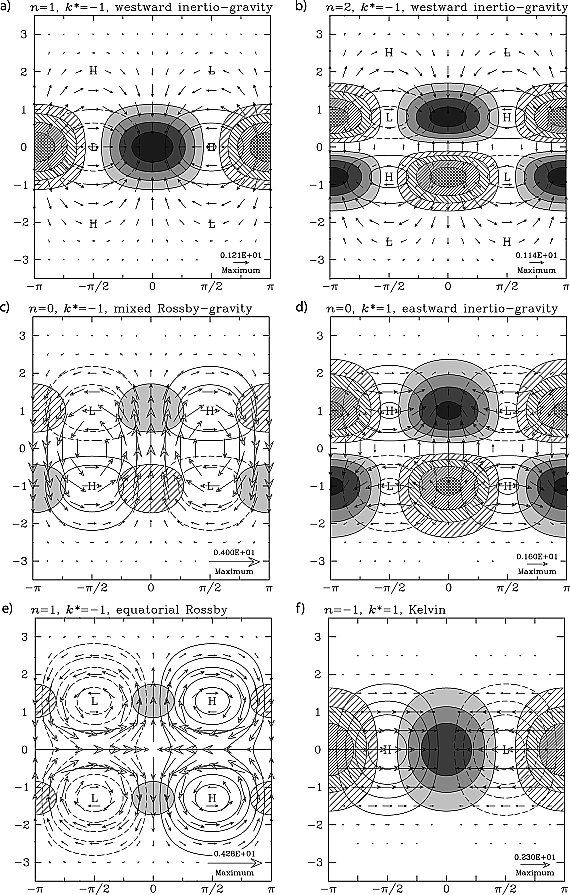
\includegraphics[height=0.7\textheight]{graphics/rog1687-fig-0003.png}\\
\textit{Horizontal structures of selected zonally propagating wave solutions to the shallow water equations on an equatorial $\beta$ plane. (Kiladis et al., 2009)}
\end{solution}

\section{Python Programming}
Here we demonstrate how to compute a real inner product supplied by a symmetric bilinear form $B$ and carry out Gram-Schmidt Orthogonalization with respect to it. We use Example \ref{exmp:R3innerGS} as the test case. We first define a function to calculate the inner product given two input vectors and the matrix $B$:
\begin{lstlisting}
import numpy as np

def real_inner_prod(u, v, B):
    if np.all(B == B.T): # Check if symmetric
        return(u @ B @ v)
    else:
        print("Not symmetric bilinear form!")
        return(None)   
\end{lstlisting}
Let's check it with that $B$ in Example \ref{exmp:R3innerGS} and $\vec{u} = (1,0,1)^T$, $\vec{v} = (0,2,-1)^T$. Then
\begin{lstlisting}
u = np.array([1., 0., 1.])
v = np.array([0., 2., -1.])
B = np.array([[2., 1., 0.],  
              [1., 2., 1.],
              [0., 1., 2.]])

print(real_inner_prod(u,v,B))    
\end{lstlisting}
gives \verb|2.0| which turns out to be correct. For convenience, we also define a function to compute norm, which is simply a wrapped version of \verb|real_inner_prod|:
\begin{lstlisting}
def norm(v, B):
    return(np.sqrt(real_inner_prod(v, v, B)))
\end{lstlisting}
Now comes the main part of executing the Gram-Schmidt procedure. The inner loop subtracts the parallel components of each previous vector from the current vector and the outer loop iterates the calculation for every input vector.
\begin{lstlisting}
def GS_inner_prod(vecs, B):
    """
    Gram-Schmidt Orthogonalization with respect to an inner product (finite-dimensional)
    vecs: A list containing the vectors
    B: The symmetric matrix for the inner product
    """
    n_vecs = len(vecs)
    for jj in np.arange(n_vecs):
        for ii in np.arange(jj):
            vecs[jj] -= real_inner_prod(vecs[jj], vecs[ii], B) / norm(vecs[ii], B)**2 * vecs[ii]
    return(vecs)    
\end{lstlisting}
Trying this with Example \ref{exmp:R3innerGS}
\begin{lstlisting}
vecs = [np.array([1.,0.,0.]), 
        np.array([0.,1.,0.]), 
        np.array([0.,0.,1.])]
print(GS_inner_prod(vecs, B))
\end{lstlisting}
produces
\begin{lstlisting}
[array([1., 0., 0.]), array([-0.5,  1. ,  0. ]), array([ 0.33333333, -0.66666667,  1.        ])]    
\end{lstlisting}
which matches our answer in the example.

\section{Exercises}

\begin{Exercise}
Show that the set of all $n \times n$ (complex) matrices $\mathcal{V} = \mathcal{M}_{n \times n}(\mathbb{C})$ is a vector space and the definition $\langle A, B\rangle = \text{tr}(AB^*)$ satisfies the requirements of an inner product for this vector space. This form of inner product is better known as the \textit{Frobenius inner product}.
\end{Exercise}

\begin{Exercise}
Show that $\vec{u} = (-1,0,2)^T$ and $\vec{v} = (1,-1,1)^T$ in $\mathbb{R}^3$ are orthogonal to each other if an inner product of
\begin{align*}
\langle\vec{u}, \vec{v}\rangle = \vec{u}^TB\vec{v}
\end{align*}
where 
\begin{align*}
B = 
\begin{bmatrix}
2 & 1 & 1 \\
1 & 2 & 1 \\
1 & 1 & 1
\end{bmatrix}
\end{align*}
is used. Also, find the norm $\norm{\vec{u}}$ and $\norm{\vec{v}}$ of both $\vec{u}$ and $\vec{v}$ with respect to this inner product.
\end{Exercise}

\begin{Exercise}
Let $\mathcal{V} = \mathbb{R}^3$. Show that
\begin{align*}
\langle\vec{u}, \vec{v}\rangle = \vec{u}^TB\vec{v}
\end{align*}
where 
\begin{align*}
B = 
\begin{bmatrix}
3 & 1 & -1 \\ 
1 & 3 & 0 \\ 
-1 & 0 & 1
\end{bmatrix}
\end{align*}
is a valid inner product for all $\vec{u}, \vec{v} \in \mathcal{V}$ and turns $\mathcal{V}$ into an inner product space. Hence derive an orthonormal basis for $\mathbb{R}^3$ with respect to this inner product using Gram-Schmidt Orthogonalization. 
\end{Exercise}

\begin{Exercise}
\label{ex:triangular2}
Prove the Triangular Inequality
\begin{align*}
\norm{\vec{u} + \vec{v}} \leq \norm{\vec{u}} + \norm{\vec{v}}
\end{align*}
as in Exercise \ref{ex:triangular} but now for any inner product.
\end{Exercise}

\begin{Exercise}
Show that $x^3$ and $\cos(2x)$ are orthogonal to each other in the $L^2[-\pi, \pi]$ space with respect to the inner product of Equation (\ref{eqn:integralinner}).
\end{Exercise}

\begin{Exercise}
Find the adjoint of $\mathcal{L}[f] = \frac{d}{dx}(x\frac{d}{dx}[f])$ with respect to the inner product of Equation (\ref{eqn:integralinner2})
\begin{align*}
\langle f,g \rangle = \int_a^b w(x) f(x) \overline{g(x)} dx    
\end{align*}
where $w(x) =$ (a) $1$, and (b) $e^{-x}$, with $a > 0$.
\end{Exercise}

\begin{Exercise}
Show that given a real inner product induced by $\langle \vec{u},\vec{v} \rangle = \vec{u}^TB\vec{v}$ where
\begin{align*}
B = 
\begin{bmatrix}
1 & 1 \\
1 & 2
\end{bmatrix}
\end{align*}
The linear operator that has a matrix representation of
\begin{align*}
T = 
\begin{bmatrix}
2 & 1 \\
0 & 1
\end{bmatrix}
\end{align*}
is self-adjoint.
\end{Exercise}

\begin{Exercise}
Find the Fourier series of (a) $x^2$, (b) $x^3$ and (c) $4+\sin(3x)+2\cos(8x)$ over $[-\pi, \pi]$.
\end{Exercise}

\begin{Exercise}
Convert the \textit{Legendre's Equation}
\begin{align*}
(1-x^2) y'' - 2xy' + \lambda y = 0
\end{align*}
into the Sturm-Liouville form, what should be the natural interval such that the corresponding Sturm-Liouville operator is Hermitian? Then, show that when $\lambda = n(n+1)$, $n$ is a non-negative integer, the series solution truncates and produces the \textit{Legendre polynomials} as its eigenfunctions. Find the first five of them. Alternatively, apply the Gram-Schmidt procedure over the standard polynomial basis over the natural interval to come up with the same set of Legendre polynomials.
\end{Exercise}
\chapter{Least-Square Approximation}
\label{chap:leastsq}

As discussed in Chapter \ref{chap:SolLinSys}, given a linear system, if the number of equations (rows) is greater than the number of unknowns (columns), then it is overdetermined. Generally, it would be inconsistent and there will be no solution. However, we can salvage this by finding an approximated solution such that the so-called squared error is minimized. This is known as the \textit{least-square approximation}. Its most common application is \textit{linear regression} in which we predict a dependent variable using an optimized linear equation in some independent variable(s).

\section{Mathematical Ideas of Least-Square Approximation}

For a linear system $A\vec{x} = \vec{h}$ where $\vec{h}$ does not lie in $\mathcal{C}(A)$ the column space of $A$, by Properties \ref{proper:consistentcolspace} it is inconsistent and there will be no exact solution. Nevertheless, a best-fit vector $\vec{x}_f$ can be found, where $A\vec{x}_f = \smash{\vec{h}_f}$, in the sense that $\smash{\vec{h}_f}$ will be the closest vector in the column space of $A$ to $\smash{\vec{h}}$ in distance, i.e.\ the squared error
\begin{align}
\norm{\vec{h}-\vec{h}_f}^2 = \norm{\vec{h}-A\vec{x}_f}^2    
\end{align}
is minimized and $\smash{\vec{h}_f} = A\vec{x}_f$ (or $\vec{x}_f$) is referred to as the \index{Least-square Approximation}\keywordhl{least-square approximation} to the system. From Properties \ref{proper:shortestorthoproj}, we know that the shortest distance will be achieved by the orthogonal projection of $\vec{h}$ onto the column space of $A$. Notice that the distance and orthogonality can now be defined with respect to a general inner product other than the usual dot product. Therefore, $\vec{h}-A\vec{x}_f$ will be in the orthogonal complement $\mathcal{C}(A)^\perp$\footnote{which may not be equal to $\mathcal{N}(A^T)$ or $\mathcal{N}(A^*)$ but rather $\mathcal{N}(A^\dag)$ if an inner product other than the standard one is used.} of the column space $\mathcal{C}(A)$ of $A$, and we have
\begin{align}
\langle A\vec{x}, \vec{h}-A\vec{x}_f \rangle = \langle \vec{x}, A^\dag(\vec{h}-A\vec{x}_f) \rangle = 0 
\end{align}
Since this holds for any $\vec{x}$, by the last item of Properties \ref{proper:innerprod2} we have
\begin{align}
A^\dag(\vec{h}-A\vec{x}_f) &= \textbf{0} \nonumber \\
A^\dag A\vec{x}_f &= A^\dag \vec{h}
\end{align}
This is called the \index{Normal Equation}\keywordhl{normal equation} due to the appearance of $A^\dag A$. So any $\vec{x}_f$\footnote{The existence of at least one of such a vector is guaranteed by the uniqueness of orthogonal projection of $\smash{\vec{h}}$ onto $\mathcal{C}(A)$.} satisfying this equation will produce the least-square error. We may be tempted to multiply both sides of the equation by the inverse $(A^\dag A)^{-1}$ to arrive at a formula for the least-square solution $\vec{x}_f = (A^\dag A)^{-1}A^\dag \smash{\vec{h}}$. However, this is only allowed when this inverse indeed exists, and we now discuss under what condition it will happen.\par
\begin{figure}[ht!]
    \centering
    \begin{tikzpicture}[rotate=0]
    \filldraw[fill=Green!20]
    (0,0,0) -- (4,0,0) -- (4,0,4) -- (0,0,4) -- cycle;
    \draw[red, thick, ->] (1,0,1) -- (3,2,2) node[right]{$\vec{h}$};
    \draw[blue, thick, ->] (1,0,1) -- (3,0,2) node[right]{$A\vec{x_f} = \vec{h_f}$};
    \draw[gray, thick, dashed] (3,2,2) -- (3,0,2);
    \node[Green] at (-2,0,1) {Column space of $A$};
    \end{tikzpicture}
    \caption{\textit{Geometric view for the least-square approximation problem, where $\smash{\vec{h}}$ and the orthogonal projection of $\smash{\vec{h}}$ onto the two-dimensional column space of the $3 \times 2$ matrix $A$, that is, $\smash{\vec{h_f}} = A\vec{x_f}$, are $\mathbb{R}^3$ vectors.}}
\end{figure}

\begin{proper}
For an $m \times n$ matrix $A$, $A^\dag A$ and $A$ have the same null space.
\end{proper}
\begin{proof}
It is obvious that if $\vec{x} \in \mathcal{N}(A)$, $A\vec{x} = \textbf{0}$ then $A^\dag A\vec{x} = \textbf{0}$ so $\vec{x} \in \mathcal{N}(A^\dag A)$ and $\mathcal{N}(A) \subseteq \mathcal{N}(A^\dag A)$. Now we only need to show that $\mathcal{N}(A^\dag A) \subseteq \mathcal{N}(A)$. For $\vec{x} \in \mathcal{N}(A^\dag A)$, we have $A^\dag A\vec{x} = \textbf{0}$ and hence $\langle \vec{x}, A^\dag A\vec{x} \rangle = 0$. Subsequently by the definition of an adjoint (Definition \ref{defn:adjoint}), we have $\langle A\vec{x}, A\vec{x} \rangle = \norm{A\vec{x}}^2 = 0$. By Definition \ref{defn:innerprod}, we conclude that it must be $A\vec{x} = \textbf{0}$ so $\vec{x} \in \mathcal{N}(A)$, and thus $\mathcal{N}(A^\dag A) \subseteq \mathcal{N}(A)$. Hence $\mathcal{N}(A^\dag A) = \mathcal{N}(A)$, the null space of $A^\dag A$ and $A$ coincides.
\end{proof}

\begin{proper}
\label{proper:AdagArank}
For an $m \times n$ matrix $A$, $A^\dag A$ has the same rank as $A$. As a corollary, if $A$ has linearly independent columns such that $\text{rank}(A) = n$, then $A^\dag A$ is invertible.
\end{proper}
\begin{proof}
By the Rank-nullity Theorem \ref{thm:ranknullity}, $\text{rank}(A^\dag A) + \text{nullity}(A^\dag A) = n = \text{rank}(A) + \text{nullity}(A)$ but by the previous properties $\text{nullity}(A^\dag A) = \text{nullity}(A)$ so $\text{rank}(A^\dag A) = \text{rank}(A)$ where $A^\dag A$ is an $n \times n$ matrix. Therefore if $\text{rank}(A^\dag A) = \text{rank}(A) = n$, then $A^\dag A$ is full-rank and by Properties \ref{proper:invertrank} it is invertible.
\end{proof}
Therefore, we have the following result.
\begin{thm}
\label{thm:bestfit}
If $A$ is a $m \times n$ matrix with $m \geq n$ and all its $n$ column vectors are linearly independent, then for the system $A\vec{x} = \smash{\vec{h}}$, there exists a unique best-fit solution
\begin{align}
\vec{x}_f &= (A^\dag A)^{-1}A^\dag \vec{h} \label{eqn:bestfit}
\end{align}
such that the square error $\norm{\vec{h}-\vec{h_f}}^2 = \norm{\vec{h}-A\vec{x_f}}^2$ is minimized.
\end{thm}
Notice that if $\vec{h}$ already lies in the column space of $A$, then $A\vec{x} = \vec{h}$ will have an exact solution, and the best-fit solution will be identical to this exact solution. However, on the other extreme, if the column vectors in $A$ are not linearly independent, then the best-fit solution will not be unique. Rather, the normal equation will still be consistent, but there are infinitely many possible solutions, each having the same least-square error. Also, if the standard real inner product is used so that $A^\dag = A^T$ and we by chance have the QR decomposition of $A$, then
\begin{align}
\vec{x_f} &= (A^TA)^{-1}A^T\vec{h} \nonumber \\
&= ((QR)^T(QR))^{-1}(QR)^T\vec{h} \nonumber \\
&= (R^TQ^TQR)^{-1} (QR)^T\vec{h} \nonumber \\
&= (R^TR)^{-1} R^TQ^T \vec{h} \nonumber \\
&= R^{-1} (R^T)^{-1} R^TQ^T \vec{h} \nonumber \\
&= R^{-1} Q^T\vec{h}
\end{align}
where $Q^TQ = I$ since $Q$ is an orthogonal matrix in which the column vectors form an orthonormal basis as indicated by Properties \ref{proper:QRdecompose}.

\begin{exmp}
Find the least-square solution to the overdetermined linear system
\begin{align*}
\begin{bmatrix}
1 & 2 \\
3 & 4 \\
1 & 4
\end{bmatrix}
\begin{bmatrix}
x \\
y
\end{bmatrix}
=
\begin{bmatrix}
3 \\
8 \\
7
\end{bmatrix}
\end{align*}
where the error is calculated with respect to the usual Euclidean distance, and also relative to the inner product as defined in Example \ref{exmp:R3innerGS}.
\end{exmp}
\begin{solution}
If the standard inner product is used for defining lengths, then the least-square solution in Theorem \ref{thm:bestfit} is reduced to
\begin{align*}
\vec{x}_f &= (A^TA)^{-1}A^T\vec{h} \\
&= 
\left(\begin{bmatrix}
1 & 2 \\
3 & 4 \\
1 & 4
\end{bmatrix}^T
\begin{bmatrix}
1 & 2 \\
3 & 4 \\
1 & 4
\end{bmatrix}\right)^{-1}
\begin{bmatrix}
1 & 2 \\
3 & 4 \\
1 & 4
\end{bmatrix}^T
\begin{bmatrix}
3 \\
8 \\
7
\end{bmatrix} \\
&=
\begin{bmatrix}
11 & 18 \\
18 & 36 
\end{bmatrix}^{-1}
\begin{bmatrix}
1 & 3 & 1\\
2 & 4 & 4
\end{bmatrix}
\begin{bmatrix}
3 \\
8 \\
7
\end{bmatrix} \\
&=
\begin{bmatrix}
\frac{1}{2}&-\frac{1}{4}\\
-\frac{1}{4}&\frac{11}{72}
\end{bmatrix}
\begin{bmatrix}
1 & 3 & 1\\
2 & 4 & 4
\end{bmatrix}
\begin{bmatrix}
3 \\
8 \\
7
\end{bmatrix}
=
\begin{bmatrix}
\frac{1}{2} \\
\frac{19}{12}
\end{bmatrix}
\end{align*}
and the least-square error is
\begin{align*}
\norm{\vec{h}-A\vec{x_f}}^2 &=
\norm{\begin{bmatrix}
3 \\
8 \\
7
\end{bmatrix}-
\begin{bmatrix}
1 & 2 \\
3 & 4 \\
1 & 4
\end{bmatrix}
\begin{bmatrix}
\frac{1}{2} \\
\frac{19}{12}
\end{bmatrix}
}^2 \\
&= 
\norm{\begin{bmatrix}
3 \\
8 \\
7
\end{bmatrix}-
\begin{bmatrix}
\frac{11}{3}\\
\frac{47}{6}\\ 
\frac{41}{6}
\end{bmatrix}
}^2 \\
&= 
\norm{\begin{bmatrix}-\frac{2}{3}\\ 
\frac{1}{6}\\ 
\frac{1}{6}\end{bmatrix}}^2 = (-\frac{2}{3}, \frac{1}{6}, \frac{1}{6})^T \cdot (-\frac{2}{3}, \frac{1}{6}, \frac{1}{6})^T = \frac{1}{2}
\end{align*}
For the inner product in Example \ref{exmp:R3innerGS}, an appropriate adjoint, adapted from Section \ref{section:adjointdef}, to be used in this situation is
\begin{align*}
A^\dag &= C^{-1} A^T B \\
&=
\begin{bmatrix}
1 & 0 \\
0 & 1
\end{bmatrix}^{-1}
\begin{bmatrix}
1 & 3 & 1\\
2 & 4 & 4
\end{bmatrix}
\begin{bmatrix}
2&1&0\\ 
1&2&1\\
0&1&2
\end{bmatrix} \\
&=
\begin{bmatrix}
5&8&5\\ 
8&14&12
\end{bmatrix}
\end{align*}
where $C$ can be picked to be any positive-definite matrix\footnote{The choice of $C$ actually matters if there are multiple least-square solutions and $\vec{x}_f$ is also required to have a minimal norm with respect to some other inner product. This will be explored in Section \ref{section:SVDgeneral}.} and we choose $C = I$ for simplicity. Subsequently, the least-square solution is
\begin{align*}
\vec{x}_f &= (A^\dag A)^{-1}A^\dag \vec{h} \\
&=
\left(\begin{bmatrix}
5&8&5\\ 
8&14&12
\end{bmatrix}
\begin{bmatrix}
1 & 2 \\
3 & 4 \\
1 & 4
\end{bmatrix}\right)^{-1}
\begin{bmatrix}
5&8&5\\ 
8&14&12
\end{bmatrix}
\begin{bmatrix}
3 \\
8 \\
7
\end{bmatrix} \\
&=
\begin{bmatrix}
34&62\\ 
62&120
\end{bmatrix}^{-1}
\begin{bmatrix}
5&8&5\\ 
8&14&12
\end{bmatrix}
\begin{bmatrix}
3 \\
8 \\
7
\end{bmatrix} \\
&= 
\begin{bmatrix}
\frac{30}{59}&-\frac{31}{118}\\ 
-\frac{31}{118}&\frac{17}{118}
\end{bmatrix}
\begin{bmatrix}
5&8&5\\ 
8&14&12
\end{bmatrix}
\begin{bmatrix}
3 \\
8 \\
7
\end{bmatrix}
=
\begin{bmatrix}
\frac{10}{59} \\
\frac{103}{59}
\end{bmatrix}
\end{align*}
with the least-square error being
\begin{align*}
\norm{\vec{h}-A\vec{x_f}}^2 &=
(\vec{h}-A\vec{x_f})^T B (\vec{h}-A\vec{x_f})\\
&=
\left(\begin{bmatrix}
3 \\
8 \\
7
\end{bmatrix}-
\begin{bmatrix}
1 & 2 \\
3 & 4 \\
1 & 4
\end{bmatrix}
\begin{bmatrix}
\frac{10}{59} \\
\frac{103}{59}
\end{bmatrix}\right)^T
\begin{bmatrix}
2&1&0\\ 
1&2&1\\
0&1&2
\end{bmatrix}
\left(\begin{bmatrix}
3 \\
8 \\
7
\end{bmatrix}-
\begin{bmatrix}
1 & 2 \\
3 & 4 \\
1 & 4
\end{bmatrix}
\begin{bmatrix}
\frac{10}{59} \\
\frac{103}{59}
\end{bmatrix}\right) \\
&=
\begin{bmatrix}
-\frac{39}{59}\\ 
\frac{30}{59}\\ 
-\frac{9}{59}
\end{bmatrix}^T
\begin{bmatrix}
2&1&0\\ 
1&2&1\\
0&1&2
\end{bmatrix}
\begin{bmatrix}
-\frac{39}{59}\\ 
\frac{30}{59}\\ 
-\frac{9}{59}
\end{bmatrix}
= \frac{36}{59}
\end{align*}
\end{solution}
We close this section by confirming that the matrix $T = A(A^\dag A)^{-1}A^\dag$ as in $\vec{h}_f = A\vec{x}_f = A(A^\dag A)^{-1}A^\dag \vec{h}$ indeed represents an orthogonal projection (of $\vec{h}$ onto the column space of $A$). By Properties \ref{proper:orthoprojadjoint} we just need to check if $T^2 = T = T^\dag$. For the first equality, we have
\begin{align*}
T^2 &= (A(A^\dag A)^{-1}A^\dag)(A(A^\dag A)^{-1}A^\dag) \\
&= A(A^\dag A)^{-1}(A^\dag A)(A^\dag A)^{-1}A^\dag \\
&= A(A^\dag A)^{-1}(I)A^\dag = A(A^\dag A)^{-1}A^\dag = T
\end{align*}
and for the second equality, we can use Properties \ref{proper:adjoints} to get
\begin{align*}
T^\dag &= (A(A^\dag A)^{-1}A^\dag)^\dag \\
&= (A^\dag)^\dag((A^\dag A)^{-1})^\dag A^\dag \\
&= A ((A^\dag A)^\dag)^{-1} A^\dag \\
&= A (A^\dag A)^{-1} A^\dag = T
\end{align*}

\section{Linear Regression}
\subsection{Linear Regression for One Predictor Variable}

\index{Linear Regression}\keywordhl{Linear regression} is a very important tool in Statistics that helps identify any linear trend in data and is based on least-square approximation. The simplest type of linear regression is fitting a straight line $y = \alpha + \beta x$, where $\alpha$ and $\beta$ are its intercept and slope, to $m$ pairs of observation, $(x_1, y_1), (x_2, y_2), \cdots, (x_m, y_m)$ such that the sum of squared errors $\sum_{k=1}^m (y_k - (\alpha + \beta x_k))^2$ is minimized. In this context, $x$ and $y$ are known as the \textit{explanatory} and \textit{response variable} respectively.\par

\begin{figure}[ht!]
\centering
\begin{tikzpicture}
\draw[thick, ->] (-1,0) -- (5,0) node[right]{$x$};
\draw[thick, ->] (0,-1) -- (0,5) node[above]{$y$};
\node[circle, inner sep=1pt, fill=blue] at (1,1.2) {};
\node at (0.8,1.6) {$(1,1.2)$};
\node[circle, inner sep=1pt, fill=blue] at (2,1.6) {};
\node at (2.2,1.2) {$(2,1.6)$};
\node[circle, inner sep=1pt, fill=blue] at (3,2.8) {};
\node at (3.2,2.4) {$(3,2.8)$};
\node[circle, inner sep=1pt, fill=blue] at (4,4.4) {};
\node at (3.8,4.8) {$(4,4.4)$};
\draw[thick, red] (-0.5,-0.74) -- (5,5.2) node[right]{$y = -0.2+1.08x$};
\node[below left]{$O$}; 
\draw[thick, Green] (1,1.2) -- (1,0.88);
\draw[thick, Green] (2,1.6) -- (2,1.96);
\draw[thick, Green] (3,2.8) -- (3,3.04);
\draw[thick, Green] (4,4.4) -- (4,4.12);
\end{tikzpicture}
\caption{\textit{A toy linear regression model for 4 data points. The red straight line represents the best linear fit, and the green lines are the distances, or errors between the actual data and the regression line, whose sum of squares is minimized.}}
\end{figure}

To see how we can apply the results in the last section, we first rewrite the system into matrix form. The actual sampled values are given by $\vec{y} = (y_1, y_2, \ldots, y_m)^T$, while the values predicted by the best-fit straight line will be in the form of $\vec{y}^{\text{pred}} = (\alpha\textbf{1} + \beta \vec{x})^T = (\alpha + \beta x_1, \alpha + \beta x_2, \ldots, \alpha + \beta x_m)^T$, where $\textbf{1}$ is a column vector filled with ones, $\alpha$ and $\beta$ are the intercept and slope of the best-fit line to be determined. In other words, we are trying to find an optimal solution for the unknown parameters $\alpha$ and $\beta$ in the matrix system
\begin{align}
\alpha\textbf{1} + \beta \vec{x} &= \vec{y}
\end{align}
or alternatively
\begin{align}
\begin{bmatrix}
1 & x_1 \\
1 & x_2 \\
\vdots & \vdots \\
1 & x_m
\end{bmatrix}
\begin{bmatrix}
\alpha \\
\beta
\end{bmatrix}
=
\begin{bmatrix}
y_1 \\
y_2 \\
\vdots \\
y_m
\end{bmatrix}
\end{align}
so that the sum of squared errors $\smash{\sum_{k=1}^m (y_k - y^{\text{pred}}_k)^2} = \sum_{k=1}^m (y_k - (\alpha + \beta x_k))^2$ is minimized. Such a system is conveniently denoted as $[X]\vec{\beta} = \vec{y}$, where the first and second column of $[X] = [\textbf{1}|\vec{x}]$ represent the two predictors, the constant term which is a "hidden" predictor that gives rise to the $y$-intercept, and the linear term of $x$. Now, the sum of squared errors
\begin{align}
\sum_{k=1}^m (y_k - (\alpha + \beta x_k))^2 = \norm{\vec{y} - [X]\vec{\beta}}^2    
\end{align}
will be minimized by the best-fit parameters which are computed via
\begin{align}
\vec{\beta_f} = ([X]^T[X])^{-1}[X]^T \vec{y}
\end{align}
according to Theorem \ref{thm:bestfit} where $A = [X]$, and simply $A^\dag = [X]^T$ as the error is computed based on the usual dot product/Euclidean distance. Writing out the matrices in the formula, the parameters for single variable linear regression are
\begin{align}
\begin{bmatrix}
\alpha_f \\
\beta_f
\end{bmatrix}
&=
\left(
\begin{bmatrix}
1 & 1 & \cdots & 1 \\
x_1 & x_2 & \cdots & x_m
\end{bmatrix}
\begin{bmatrix}
1 & x_1 \\
1 & x_2 \\
\vdots & \vdots \\
1 & x_m
\end{bmatrix} 
\right)^{-1}
\begin{bmatrix}
1 & 1 & \cdots & 1 \\
x_1 & x_2 & \cdots & x_m
\end{bmatrix}
\begin{bmatrix}
y_1 \\
y_2 \\
\vdots \\
y_m
\end{bmatrix} \nonumber \\
&= 
\begin{bmatrix}
m & \sum X \\
\sum X & \sum X^2
\end{bmatrix}^{-1}
\begin{bmatrix}
\sum Y \\
\sum XY
\end{bmatrix} \nonumber  \\
&=
\frac{1}{m(\sum X^2) - (\sum X)^2}
\begin{bmatrix}
\sum X^2 & -\sum X \\
-\sum X & m
\end{bmatrix}
\begin{bmatrix}
\sum Y \\
\sum XY
\end{bmatrix} \nonumber \\
&=
\frac{1}{m(\sum X^2) - (\sum X)^2}
\begin{bmatrix}
(\sum Y) (\sum X^2) - (\sum X) (\sum XY) \\
m (\sum XY) - (\sum X) (\sum Y)
\end{bmatrix}
\end{align}
where 
\begin{subequations}
\begin{align}
\sum X &= x_1 + x_2 + \cdots + x_m \\
\sum X^2 &= x_1^2 + x_2^2 + \cdots + x_m^2 \\
\sum Y &= y_1 + y_2 + \cdots + y_m \\
\sum XY &= x_1y_1 + x_2y_2 + \cdots + x_my_m   
\end{align}
\end{subequations}
and we have used the results (\ref{eqn:2times2inv}) in Example \ref{exmp:2x2} to calculate the inverse from the second to third line.
\begin{proper}
\label{proper:bestfit2}
The best-fit parameters for the single predictor variable linear regression are found by
\begin{subequations}
\label{eqn:bestfit2}
\begin{align}
\alpha_f &= \frac{(\sum Y) (\sum X^2) - (\sum X) (\sum XY)}{m(\sum X^2) - (\sum X)^2} \\
\beta_f &= \frac{m (\sum XY) - (\sum X) (\sum Y)}{m(\sum X^2) - (\sum X)^2}
\end{align}    
\end{subequations}
such that the regression line $y = \alpha_f + \beta_f x$ achieves the least-square error, i.e.\ the value of $\sum_{k=1}^m (y_k - (\alpha_f + \beta_f x_k))^2$ is the smallest possible.
\end{proper}
\begin{exmp}
\label{ex11.1.1}
Find the best linear fit for five $(x,y)$ data points, which are $(2,4)$, $(3,6)$, $(4,7)$, $(5,9)$, $(7,11)$.
\end{exmp}
\begin{solution}
We first compute the following quantities.
\begin{align*}
\sum X &= 2+3+4+5+7 = 21 \\
\sum(X^2) &= 2^2+3^2+4^2+5^2+7^2 = 103 \\
\sum Y &= 4+6+7+9+11 = 37 \\
\sum (XY) &= (2)(4)+(3)(6)+(4)(7)+(5)(9)+(7)(11) = 176
\end{align*}
By Formula (\ref{eqn:bestfit2}) in Properties \ref{proper:bestfit2}, with $m=5$, the required parameters are
\begin{align*}
\alpha_f &= \frac{\sum Y \sum (X^2) - \sum X \sum (XY)}{m\sum(X^2) - (\sum X)^2} = \frac{(37)(103)-(21)(176)}{(5)(103)-(21)^2} \approx 1.554 \\
\beta_f &= \frac{m \sum(XY) - (\sum X) (\sum Y)}{m\sum(X^2) - (\sum X)^2} = \frac{(5)(176)-(21)(37)}{(5)(103)-(21)^2} \approx 1.392
\end{align*}
So the best linear fit is around $y = 1.554 + 1.392x$.
\end{solution}

\subsection{Linear Regression for Multiple Predictor Variables}

Sometimes we may need to predict a variable $y$ with multiple predictor variables $x^{(1)}, x^{(2)}, \ldots, x^{(n)}$ as there can be different factors contributing to a phenomenon in any Earth Science scenario. Linear regression for multiple predictor variables will then produce a best-fit equation in the form of $y = \alpha + \beta_1x^{(1)} + \beta_2x^{(2)} + \cdots + \beta_nx^{(n)}$. Extending the earlier results from Theorem \ref{thm:bestfit}, the computation of the parameters utilizes the same formula
\begin{align*}
\vec{\beta}_f = ([X]^T[X])^{-1}[X]^T \vec{y}
\end{align*}
where in this case the quantities now involve more predictor variables, $\smash{\vec{\beta}_f^T} = \smash{(\alpha_f, {\beta_1}_f, {\beta_2}_f, \cdots, {\beta_n}_f)^T}$, and the matrix $[X] = [\textbf{1}|\vec{x}^{(1)}|\vec{x}^{(2)}|\cdots|\vec{x}^{(n)}]$ holds the observed values of those multiple predictor variables column by column.

\begin{exmp}
\label{exmp:GPAregress}
The university carries out an experiment and tries to quantify the effects of IQ and studying time on the GPA of students. 5 students participated and the data are shown below.
\begin{center}
\begin{tabular}{|c|c|c|c|}
\hline
Students & IQ & Studying Time per Week (Hours) & GPA \\
\hline
Lily & $104$ & $5.2$ & $3.56$ \\
\hline
Christy & $111$ & $6.1$ & $3.71$ \\
\hline
Sabrina & $107$ & $8.3$ & $3.73$ \\
\hline
Julia & $106$ & $3.4$ & $3.34$ \\
\hline
Emily & $109$ & $9.6$ & $3.88$ \\
\hline
\end{tabular}
\end{center} 
Do a linear regression on the students' GPA against their IQ and studying time.
\end{exmp}
\begin{solution}
Denote the IQ and studying hours of the students by the variables $x^{(1)}$ and $x^{(2)}$, and $y$ for their GPA, we want to fit a linear relationship $y = \alpha + \beta_1 x^{(1)} + \beta_2 x^{(2)}$. The matrix $[X] = [\textbf{1}|\vec{x}^{(1)}|\vec{x}^{(2)}] $, consisting of the observed predictors, is then
\begin{align*}
[X] = \left[
\begin{array}{ccc}
1 & 104 & 5.2 \\
1 & 111 & 6.1 \\
1 & 107 & 8.3 \\
1 & 106 & 3.4 \\
1 & 109 & 9.6
\end{array}
\right]
\end{align*}
The first column represents the intercept term. Subsequently, the fit is derived by
\begin{align*}
\vec{\beta}_f &= ([X]^T [X])^{-1} [X]^T \vec{y} \\
&= \left(\left[
\begin{array}{ccc}
1 & 104 & 5.2 \\
1 & 111 & 6.1 \\
1 & 107 & 8.3 \\
1 & 106 & 3.4 \\
1 & 109 & 9.6
\end{array}
\right]^T
\left[
\begin{array}{ccc}
1 & 104 & 5.2 \\
1 & 111 & 6.1 \\
1 & 107 & 8.3 \\
1 & 106 & 3.4 \\
1 & 109 & 9.6
\end{array}
\right]\right)^{-1}
\left[
\begin{array}{ccc}
1 & 104 & 5.2 \\
1 & 111 & 6.1 \\
1 & 107 & 8.3 \\
1 & 106 & 3.4 \\
1 & 109 & 9.6
\end{array}
\right]^T
\left[
\begin{array}{c}
3.56 \\
3.71 \\
3.73 \\
3.34 \\
3.88
\end{array}
\right] \\
&\approx
\left[
\begin{array}{c}
1.4463 \\
0.0162 \\
0.0710 \\
\end{array}
\right] 
\end{align*}
So the regression model is $\text{GPA} = 1.4463 + 0.0162(\text{IQ}) + 0.0710(\text{Studying Hrs})$. 
\end{solution}

\begin{exmp}
Find a quadratic fit for Example \ref{ex11.1.1}.
\end{exmp}
\begin{solution}
The predictor variables are the constant term, the linear term $x$, as well as the newly added quadratic term $x^2$. The desired parameters are
\begin{align*}
\vec{\beta_f} &= ([X]^T[X])^{-1}[X]^T \vec{y} \\
&=
\left(
\begin{bmatrix}
1 & 1 & 1 & 1 & 1 \\
2 & 3 & 4 & 5 & 7 \\
2^2 & 3^2 & 4^2 & 5^2 & 7^2
\end{bmatrix}
\begin{bmatrix}
1 & 2 & 2^2 \\
1 & 3 & 3^2 \\
1 & 4 & 4^2 \\
1 & 5 & 5^2 \\
1 & 7 & 7^2 
\end{bmatrix}
\right)^{-1}
\begin{bmatrix}
1 & 1 & 1 & 1 & 1 \\
2 & 3 & 4 & 5 & 7 \\
2^2 & 3^2 & 4^2 & 5^2 & 7^2
\end{bmatrix}
\begin{bmatrix}
4 \\
6 \\
7 \\
9 \\
11
\end{bmatrix} \\
& \approx
\begin{bmatrix}
-0.009 \\
2.201 \\
-0.089 
\end{bmatrix}
\end{align*}
The quadratic fit is thus $y = -0.009 + 2.201x - 0.089x^2$.
\end{solution}
Notice that in the above example, although we use the quadratic term $x^2$ as a predictor, the regression is still \textit{linear} in the sense that the regression model is a \textit{linear} combination of these predictors. Usually, fitting a degree $n$ polynomials in a single variable $x$ to $m$ points, $n < m$, will involve a matrix in the form like the one above:
\begin{align}
[X]
&= 
\begin{bmatrix}
1 & x_1 & x_1^2 & \cdots & x_1^n \\
1 & x_2 & x_2^2 & \cdots & x_2^n \\
\vdots & \vdots & \vdots & & \vdots \\
1 & x_m & x_m^2 & \cdots & x_m^n \\
\end{bmatrix} 
\end{align}
This class of matrices is called \index{Vandermonde Matrix}\keywordhl{Vandermonde matrices}.\footnote{As long as $n < m$ and the sampled points $x_i$ are distinct, the columns of a Vandermonde matrix will be linearly independent.}

\subsection{Properties of Linear Regression}

Before going to the next topic, we derive some features of linear regression. The errors, or called the \index{Residual}\keywordhl{residuals} $e_i = h_i - (h_f)_i$, have a mean of zero. Using matrix notation, it means that the sum of components in the error vector $\vec{e} = \vec{h} - \vec{h_f}$ is zero. This can be seen from the very beginning of our derivation for the best-fit problem $A\vec{x} = \vec{h}$, where the condition has been $A^\dag (\vec{h} - A\vec{x}_f) = A^\dag (\vec{h} - \vec{h}_f) = \textbf{0}$. For linear regression, $A^\dag =[X]^T$ and it becomes $[X]^T\vec{e} = \textbf{0}$. However, since the first column in $[X]$ is $\textbf{1}$, the first entry in $[X]^T\vec{e}$ is just $\textbf{1} \cdot \vec{e}$, which is just the sum of errors. As $[X]^T\vec{e} = \textbf{0}$, the sum and hence the mean of errors must be zero.\par

Another property is that, if we denote the mean of $y$ as $\overline{y}$, each actual data and predicted values as $y_i$ and $\hat{y}_i = y^{\text{pred}}_i$ respectively, then
\begin{align}
\sum_i (y_i - \overline{y})^2 &= \sum_i (y_i - \hat{y}_i)^2 + \sum_i (\hat{y}_i - \overline{y})^2
\end{align}
The term on L.H.S. is called the \index{Sum of Squares Total (SST)}\keywordhl{SST/Sum of Squares Total}, while the two terms on R.H.S. are known as the \index{Sum of Squares Error (SSE)}\keywordhl{SSE/Sum of Squares Error} and \index{Sum of Squares Regression (SSR)}\keywordhl{SSR/Sum of Squares Regression}. To prove this, we expand the SST, which gives
\begin{align}
\text{SST} &= \sum_i (y_i - \overline{y})^2 \nonumber \\
&= \sum_i ((y_i - \hat{y}_i) + (\hat{y}_i - \overline{y}))^2 \nonumber \\
&= \sum_i (y_i - \hat{y}_i)^2 + \sum_i (\hat{y}_i - \overline{y})^2 + 2\sum_i ((y_i - \hat{y}_i) (\hat{y}_i - \overline{y})) \nonumber \\
&= \text{SSE} + \text{SSR} + 2\sum_i ((y_i - \hat{y}_i) (\hat{y}_i - \overline{y}))
\end{align}
The remaining step is to show that the last term equals zero. For simplicity, we work with the case of a single predictor variable so there are two parameters $\alpha$ and $\beta$ only, but it can be easily generalized to multiple predictors and $\beta_j$. Expanding the product gives
\begin{align}
\sum_i ((y_i - \hat{y}_i) (\hat{y}_i - \overline{y})) &= \sum_i (\hat{y}_i(y_i - \hat{y}_i)) - \overline{y} \sum_i (y_i - \hat{y}_i) \nonumber \\
&= \sum_i ((\alpha + \beta x_i)(y_i - \hat{y}_i)) - \overline{y} \sum_i (y_i - \hat{y}_i) \nonumber \\
&= \beta \sum_i (x_i(y_i - \hat{y}_i)) - (\overline{y} - \alpha) \sum_i (y_i - \hat{y}_i) \nonumber \\
&= \beta \sum_i (x_i e_i) - (\overline{y} - \alpha) \sum_i e_i
\end{align}
Using the same logic when we are investigating $[X]^T\vec{e} = \textbf{0}$ before, we know that
\begin{subequations}
\begin{align}
\textbf{1} \cdot \vec{e} &= \sum_i e_i = 0 \\
\vec{x} \cdot \vec{e} &= \sum_i (x_i e_i) = 0
\end{align}    
\end{subequations}
These two relations can also be derived by setting $\partial (\sum_i e_i^2)/\partial \alpha = 0$ and $\partial (\sum_i e_i^2)/\partial \beta = 0$ as the sum of squared errors reaches the minimum at the point of best-fit. Substituting this two equations readily implies that the concerned quantity $\sum_i ((y_i - \hat{y}_i) (\hat{y}_i - \overline{y})) = 0$ is zero, and thus $\text{SST} = \text{SSE} + \text{SSR}$. We repeat these two results as follows.
\begin{proper}
The mean error of any linear regression is zero. Moreover, its sum of squares total (SST) is equal to the sum of squares error (SSE) plus the sum of squares regression (SSR), i.e.\ 
\begin{subequations}
\begin{align}
\sum_i (y_i - \overline{y})^2 &= \sum_i (y_i - \hat{y}_i)^2 + \sum_i (\hat{y}_i - \overline{y})^2 \\
\text{SST} &= \text{SSE} + \text{SSR}   
\end{align}    
\end{subequations}
\end{proper}
The ratio of SSR to SST is known as the \index{Coefficient of Determination}\keywordhl{coefficient of determination} and is denoted by $R^2$ (hence sometimes we also simply call it \index{R-squared}\keywordhl{R-squared}). It is the proportion of variance in the response variable that can be explained by the predictors and thus indicates how good the linear fit is. It ranges from $0$ to $1$. The larger the value of $R^2$, the better the linear regression at predicting the target variable. If $R^2$ is close to one, then the fit is almost perfect. However, it is cautioned that there may be the problem of \textit{overfitting}\footnote{For $n$ distinct sets of data, it is always possible to achieve a perfect fit ($R^2 = 1$) using $n-1$ predictors (plus the intercept term) in the linear regression even when they may not be really related to the predictand and this is an extreme case of overfitting.}, which means that the regression does well on the dataset it is trained on but fails horribly when extrapolated to data points outside this training set. On the other hand, if $R^2$ is low, then the linear regression is ineffective, but it simply means that there is no apparent linear trend and the possibility of other forms of relationship, like a logarithmic one, existing between the explanatory variables and response variable, cannot be ruled out.

\begin{exmp}
\label{exmp:GPAregress2}
Find the R-squared for the linear regression in Example \ref{exmp:GPAregress}.
\end{exmp}
\begin{solution}
We compute the SST and SSR as follows.
\begin{align*}
\overline{y} &= \frac{1}{5}(3.56 + 3.71 + 3.73 + 3.34 + 3.88) \\
&= 3.644 \\
\text{SST} &= \sum_i (y_i - \overline{y})^2 \\
&= (3.56 - 3.644)^2 + (3.71 - 3.644)^2 + (3.73 - 3.644)^2 \\
&\quad + (3.34 - 3.644)^2 + (3.88 - 3.644)^2 \\
&\approx 0.167 \\
\text{SSR} &= \sum_i (\hat{y}_i - \overline{y})^2 \\
&= ((1.4463 + 0.0162(104)+ 0.0710(5.2)) - 3.644)^2 \\
&\quad + ((1.4463 + 0.0162(111)+ 0.0710(6.1)) - 3.644)^2 \\
&\quad + ((1.4463 + 0.0162(107)+ 0.0710(8.3)) - 3.644)^2 \\
&\quad + ((1.4463 + 0.0162(106)+ 0.0710(3.4)) - 3.644)^2 \\
&\quad + ((1.4463 + 0.0162(109)+ 0.0710(9.6)) - 3.644)^2 \\
&= (3.500 - 3.644)^2 + (3.678 - 3.644)^2 + (3.769 - 3.644)^2 \\
&\quad + (3.405 - 3.644)^2 + (3.894 - 3.644)^2 \\
&\approx 0.157
\end{align*}
Hence $R^2 \approx 0.157/0.167 = 0.94$ which indicates a good fit.
\end{solution}

\section{Earth Science Applications}

\begin{exmp}
Find the least-square approximation to the temperature measurement problem in Example \ref{exmp:weatherstats}.
\end{exmp}
\begin{solution}
In Example \ref{exmp:weatherstats2}, we have found that the corresponding overdetermined system has no exact solution. To find the least-square solution, we invoke the formula in Theorem \ref{thm:bestfit} where
\begin{align*}
\vec{x}_f &= (A^TA)^{-1}A^T\vec{h}
\end{align*}
with 
\begin{align*}
A &= 
\begin{bmatrix}
10 & 20 \\
25 & 15 \\
-10 & 5
\end{bmatrix}
& \text{and} &
& \vec{h} &= \begin{bmatrix}
0.2 \\
0.3 \\
-0.2
\end{bmatrix}
\end{align*}
So
\begin{align*}
\vec{x}_f &= 
\left(\begin{bmatrix}
10 & 20 \\
25 & 15 \\
-10 & 5
\end{bmatrix}^T
\begin{bmatrix}
10 & 20 \\
25 & 15 \\
-10 & 5
\end{bmatrix}\right)^{-1}
\begin{bmatrix}
10 & 20 \\
25 & 15 \\
-10 & 5
\end{bmatrix}^T
\begin{bmatrix}
0.2 \\
0.3 \\
-0.2
\end{bmatrix} \\
&\approx 
\begin{bmatrix}
0.01357 \\
0.00058
\end{bmatrix}
\end{align*}
So the approximated solution of the temperature gradients that minimizes the squared errors is $\partial T/\partial x = \SI{1.36e-2}{\degree C \per \km} $ and $\partial T/\partial y = \SI{0.58e-3}{\degree C \per \km}$.
\end{solution}

\section{Python Programming}

We will use Example \ref{exmp:GPAregress} to demonstrate how to do a linear regression in Python. The \verb|statsmodels| module is recommended for this. First, let's provide the data.
\begin{lstlisting}
import numpy as np
import statsmodels.api as sm

X = np.array([[104, 5.2],
              [111, 6.1],
              [107, 8.3],
              [106, 3.4],
              [109, 9.6]]) 
Y = np.array([3.56, 3.71, 3.73, 3.34, 3.88])
\end{lstlisting}
We need to append the constant term by using the \verb|sm.add_constant| function.
\begin{lstlisting}
Xc = sm.add_constant(X, prepend=False)    
\end{lstlisting}
Subsequently, create an \verb|sm.OLS| (stands for "Ordinary Least Squares") object and call the \verb|fit| method that takes the predictand/predictors in the first/second argument.
\begin{lstlisting}
mod = sm.OLS(Y, Xc)
res = mod.fit()
\end{lstlisting}
The \verb|summary| method will output a table that provides relevant parameters about the linear regression like the R-squared and p-values.
\begin{lstlisting}
print(res.summary())
\end{lstlisting}
and the \verb|predict| method will return the predicted values from an input dataset according to the linear regression.
\begin{lstlisting}
print(res.predict(Xc))    
\end{lstlisting}
This gives \verb|[3.495 3.672 3.764 3.400 3.888]| which is slightly different from what we have obtained in Example \ref{exmp:GPAregress} as our manual calculation of the regression coefficients inevitably contains more round-off errors.
\begin{figure}[ht!]
    \centering
    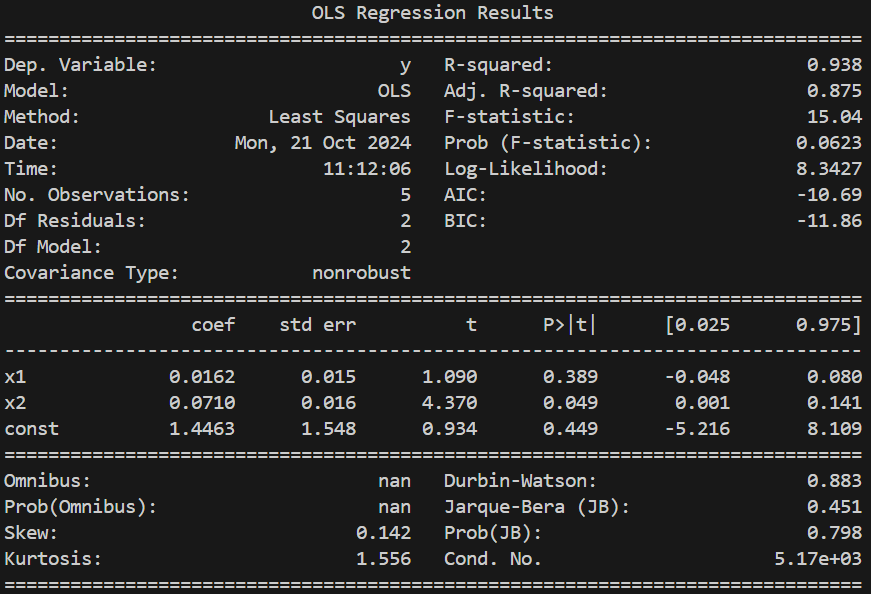
\includegraphics[width=0.99\textwidth]{graphics/OLS_table.png}
    \caption{\textit{The output of the Python program that calculates the OLS for Example \ref{exmp:GPAregress}.}}
\end{figure}

\section{Exercise}

\begin{Exercise}
Show that if $A$ is an invertible $n \times n$ square matrix then the least-square solution of $A\vec{x} = \vec{h}$ given in Theorem \ref{thm:bestfit}
\begin{align*}
\vec{x}_f &= (A^\dag A)^{-1}A^\dag \vec{h}    
\end{align*}
will be reduced to simply
\begin{align*}
\vec{x}_f &= A^{-1}\vec{h}    
\end{align*}
the exact solution as derived in Section \ref{subsection:SolLinSysInv}.
\end{Exercise}

\begin{Exercise}
Find the least-square solution to the overdetermined linear system below.
\begin{align*}
\left\{\begin{alignedat}{2}
&x + 2y - 3z &&= 4 \\
&x - y + 3z &&= 5 \\
&2x + y - z &&= 1 \\
&x + y + z &&= 2
\end{alignedat}\right.
\end{align*}
\end{Exercise}

\begin{Exercise}
Find a linear fit for the following data about sea level pressure and temperature measured at a weather station.
\begin{center}
\begin{tabular}{|c|c|c|c|c|c|c|}
\hline
Temperature ($^\circ$ C) & $10$ & $12$ & $12$ & $13$ & $16$ & $17$\\
\hline
Pressure (hPa) & $1022.1$ & $1019.5$ & $1018.9$ & $1017.6$ & $1014.3$ & $1013.5$\\
\hline
\end{tabular}
\end{center}
\end{Exercise}

\begin{Exercise}
\phantomsection
\label{ex:carbontrend}
Find a linear fit and a quadratic fit for the following atmospheric data regarding global carbon dioxide level. Also, calculate the root-mean-square error for each fit.
\begin{figure}[h!]
\centering
\fbox{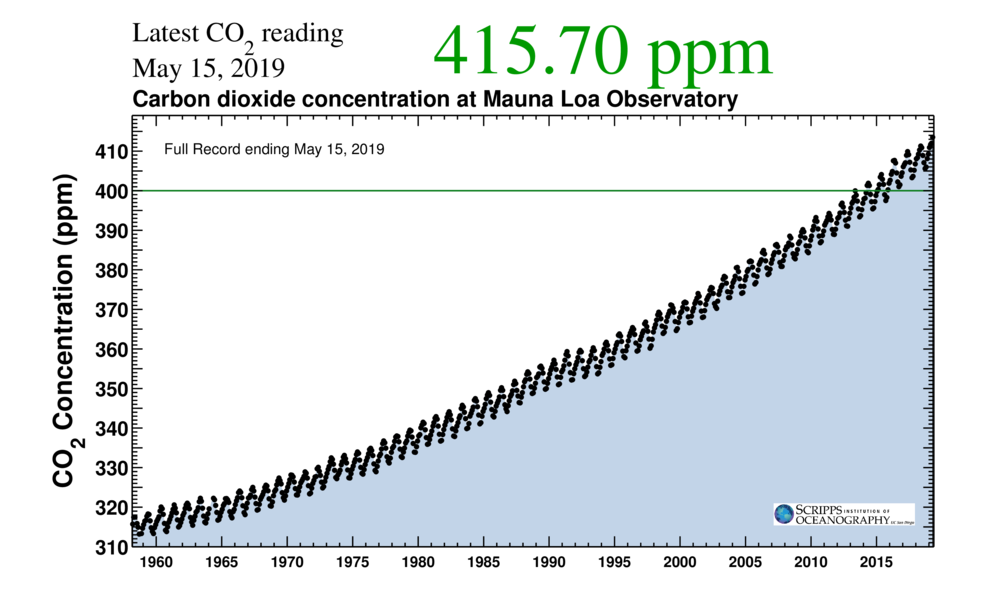
\includegraphics[scale = 0.32]{carbon.png}}
\caption{\textit{The trend of atmospheric carbon dioxide level measured at Mauna Loa Observatory for Example \ref{ex:carbontrend}.}}
\end{figure}
\begin{center}
\begin{tabular}{|c|c|c|c|c|c|c|}
\hline
Years passed since 1960 & $0$ & $5$ & $10$ & $15$ & $20$ & $25$ \\
\hline
CO$_2$ level (ppm) & $316.9$ & $320.0$ & $325.7$ & $331.1$ & $338.8$ & $346.4$ \\
\hline
Years passed since 1960 & $30$ & $35$ & $40$ & $45$ & $50$ & $55$\\
\hline
CO$_2$ level (ppm) & $354.4$ & $361.0$ & $369.7$ & $380.0$ & $390.1$ & $401.0$\\
\hline
\end{tabular}
\end{center}
(Data from: \href{https://gml.noaa.gov/webdata/ccgg/trends/co2/co2_mm_mlo.csv}{NOAA (https://gml.noaa.gov/webdata/ccgg/trends/co2/\\co2\_annmean\_mlo.csv)})
\end{Exercise}

\begin{Exercise}
Radioactive decay is modeled by $N = N_0e^{-kt}$, where $N_0$ and $k$ are the initial concentration and the decay constant respectively. While the formula is exponential, not linear, the technique of linear regression can still be applied if the data undergoes \textit{linearization}. Show that by the substitution $n = \ln N$ the equation can be transformed into a linear equation $n = \ln N = \ln N_0 - kt = n_0 - kt$. Hence find the best linear fit on $(t, n)$ by finding the parameters $(n_0, k)$ from the experimental data on the radioactive isotope Sodium-24 below and recover the decay constant and initial mass.
\begin{center}
\begin{tabular}{|c|c|c|c|c|c|c|}
\hline
Time passed (hr) & $6$ & $8$ & $12$ & $24$ & $36$ & $48$\\
\hline
Mass (g) & $75.8$ & $69.1$ & $57.3$ & $33.0$ & $18.8$ & $10.8$\\
\hline
\end{tabular}
\end{center}
\end{Exercise}

\begin{Exercise}
A commercial study investigates eight companies that sell the same type of products and are also similar in size. The following table summarizes their revenues, R\&D expenses, employee wages, and amounts of advertisement (the last three items are normalized scores).
\begin{center}
\begin{tabular}{|c|c|c|c|c|}
\hline
& Revenues & R\&D & Wages & Advertisement \\
\hline
Company 1 & $135\%$ & $2.5$ & $1.7$ & $0.8$ \\
\hline
Company 2 & $128\%$ & $1.6$ & $1.8$ & $1.5$ \\
\hline
Company 3 & $119\%$ & $1.8$ & $0.5$ & $2.4$ \\
\hline
Company 4 & $121\%$ & $0.3$ & $1.5$ & $1.2$ \\
\hline
Company 5 & $126\%$ & $1.9$ & $1.6$ & $1.3$ \\
\hline
Company 6 & $112\%$ & $0.8$ & $1.1$ & $0.2$ \\
\hline
Company 7 & $143\%$ & $2.2$ & $2.4$ & $1.1$ \\
\hline
Company 8 & $135\%$ & $1.5$ & $2.2$ & $2.3$ \\
\hline
\end{tabular}
\end{center}
Construct a linear regression model for the revenue against the three factors that follow. What is the $R^2$ of this regression?
\end{Exercise} 
\chapter{Discrete Fourier Transform (DFT)}
We now discuss a powerful mathematical tool that can be approached from a least-square approximation view point. In the last chapter, we have seen how to fit a polynomial curve to some data. It is then natural to ask further, whether there are other suitable types of curves that can be used for data fitting as well. Remember in Chapter \ref{chap:innerchap} we have derived the Fourier series which can expand any reasonable function in sines and cosines. Coincidentally, in the area of Earth Science, many phenomena can be described by the notion of \textit{waves}, which are often taken to be \textit{sinusoidal} during their derivation, e.g. atmospheric gravity wave, seismic waves, electromagnetic wave. However, in real-life our sampling of data will be discrete. Therefore, we may want to know if we can do something similar and interpolate a discrete time-series by fitting sines and cosines to it, and this is the central idea of what is known as the \textit{Discrete Fourier Transform}.

\section{Mathematical Ideas of DFT}

\subsection{From Fourier Series to a Prototype of DFT}

By Properties \ref{proper:fourierseries}, we know that any function $f(x)$ in the interval $[-\pi, \pi]$ can be written as 
\begin{align*}
f(x) = \frac{a_0}{2} + \sum_{m=1}^{\infty} a_m \cos(mx) + \sum_{n=1}^{\infty} b_n \sin(nx) 
\end{align*} where the Fourier coefficients $a_m$ and $b_n$ are given by Formulae (\ref{eqn:fouriera}) and (\ref{eqn:fourierb}). By a change of variable $x = \frac{2\pi}{N}t - \pi$, the interval is scaled to $t \in [0, N]$ where the cosines and sines are now in the form of
\begin{align*}
\cos(m(\frac{2\pi}{N}t - \pi)) &= \cos(\frac{2m\pi}{N}t) \\
\sin(n(\frac{2\pi}{N}t - \pi)) &= \sin(\frac{2n\pi}{N}t)
\end{align*}
The negative sign due to the $m\pi$ or $n\pi$ term inside is absorbed whenever needed. Since it involves a linear variable transformation only, these cosines and sines \begin{align*}
\left\{\sqrt{\frac{2}{N}}\sin(\frac{2\pi}{N}t), \sqrt{\frac{2}{N}}\sin(\frac{2\pi(2)}{N}t), \sqrt{\frac{2}{N}}\sin(\frac{2\pi(3)}{N}t), \ldots, \frac{1}{\sqrt{N}}, \right. \\ \left. \sqrt{\frac{2}{N}}\cos(\frac{2\pi}{N}t), \sqrt{\frac{2}{N}}\cos(\frac{2\pi(2)}{N}t), \sqrt{\frac{2}{N}}\cos(\frac{2\pi(3)}{N}t), \ldots \right\}    
\end{align*} are still an orthonormal basis to the new $L^2[0, N]$ space mapped from the initial $L^2[-\pi, \pi]$\footnote{Denote the original Fourier basis functions by $\varphi_j(x) \in L^2[-\pi, \pi]$. We will only show the part of linear independence and omit the justification for span and and orthogonality. By Theorem \ref{thm:linearindep}, since they form a basis as given, $c_1\varphi_j(x) + c_2\varphi_j(x) + \cdots = 0(x) \equiv 0$ where $0(x)$ is the zero function, has the trivial solution $c_j = 0$ as its only solution. Assume the form of the linear change in variable is $x = \alpha t + \beta = X(t)$. Replacing $x$ by $X(t)$ (possible since $\alpha \neq 0$) then immediately produces the equality $c_1\varphi_j(X(t)) + c_2\varphi_j(X(t)) + \cdots = 0(X(t)) \equiv 0$ which automatically inherits the desired property of possessing only the trivial solution as well and shows that the new basis functions are now $\hat{\varphi}_j(t) = \varphi_j(X(t))$.}. The Fourier coefficients are now computed by 
\begin{align}
a_m &= \frac{1}{\pi} \int_{-\pi}^{\pi} f(x)\cos(\frac{2m\pi}{N}t) d(\frac{2\pi}{N}t) = \frac{2}{N} \int_{0}^{N} f(t)\cos(\frac{2m\pi}{N}t) dt \label{eqn:fouriersca} \\
b_n &= \frac{1}{\pi} \int_{-\pi}^{\pi} f(x)\sin(\frac{2n\pi}{N}t) d(\frac{2\pi}{N}t) = \frac{2}{N} \int_{0}^{N} f(t)\sin(\frac{2n\pi}{N}t) dt \label{eqn:fourierscb}   
\end{align}
where we have written $f(t)$ in place of $f(x) = f(\frac{2\pi}{N}t - \pi)$. The partial sum of the Fourier expansion of $f(t)$ up to degree $p$
\begin{align}
S_p(t) &= \frac{a_0}{2} + \sum_{m=1}^{p} a_m \cos(\frac{2m\pi}{N}t) + \sum_{n=1}^{p} b_n \sin(\frac{2n\pi}{N}t) \label{eqn:fourierpart} \\
&= \frac{a_0}{2} + a_1 \cos(\frac{2\pi}{N}t) + a_2 \cos(\frac{2\pi(2)}{N}t) + \cdots + a_p \cos(\frac{2\pi p}{N}t) \nonumber \\
&\quad + b_1 \sin(\frac{2\pi}{N}t) + b_2 \sin(\frac{2\pi(2)}{N}t) + \cdots + b_p \sin(\frac{2\pi p}{N}t) \nonumber
\end{align}
will then be the best approximation of the function $f(t)$ using sines and cosines up to order $p$ with distance defined with respect to the inner product of Equation (\ref{eqn:integralinner}), a.k.a.\ the best-fit trigonometric polynomial of degree $p$. This is known as the \textit{Best Approximation Theorem} which directly follows from Properties \ref{proper:shortestorthoproj} and related discussion about Fourier basis in Section \ref{section:adjointherm} because such a Fourier expansion $S_p(t)$ is essentially an orthogonal projection of $f(t)$ onto the subspace spanned by the corresponding orthonormal trigonometric basis up to order $p$. Hence, higher the degree of the partial sum of the Fourier expansion, the more closer the approximation  to the given function. We use Example \ref{exmp:fourierx} as an illustration. The appropriate Fourier series of $x = f(t) = \frac{2\pi}{N}t - \pi$ is now
\begin{align*}
f(t) &= \sum_{n=1}^{\infty} b_n \sin(\frac{2n\pi}{N}t) \\
&= -2 \sum_{n=1}^{\infty} \frac{1}{n} \sin(\frac{2n\pi}{N}t)
\end{align*}
where $b_n = -\frac{2}{n}$. The following plot shows the original function as well as the partial sum of its Fourier expansion up to degree $3,10,20$. From this, we can see that as the degree $p$ goes up, $S_p(t)$ becomes a better approximation to the straight line $y = \frac{2\pi}{N}t - \pi$\footnote{Notice that at the end points, the values of Fourier series of $f(t) = \frac{2\pi}{N}t - \pi$ stay at $0$. It is because the Fourier series works as the periodic extension of the original function (see Footnote \ref{foot:fourier} in Chapter \ref{chap:innerchap}) and will converge to the average of the left and right limits $(f_-(t) + f_+(t))/2$ at point of discontinuity. Therefore, the end point is essentially a discontinuity where one of the side limits is $\pi$ while the another is $-\pi$, so it converges to $((-\pi) + \pi)/2 = 0$.}. \\
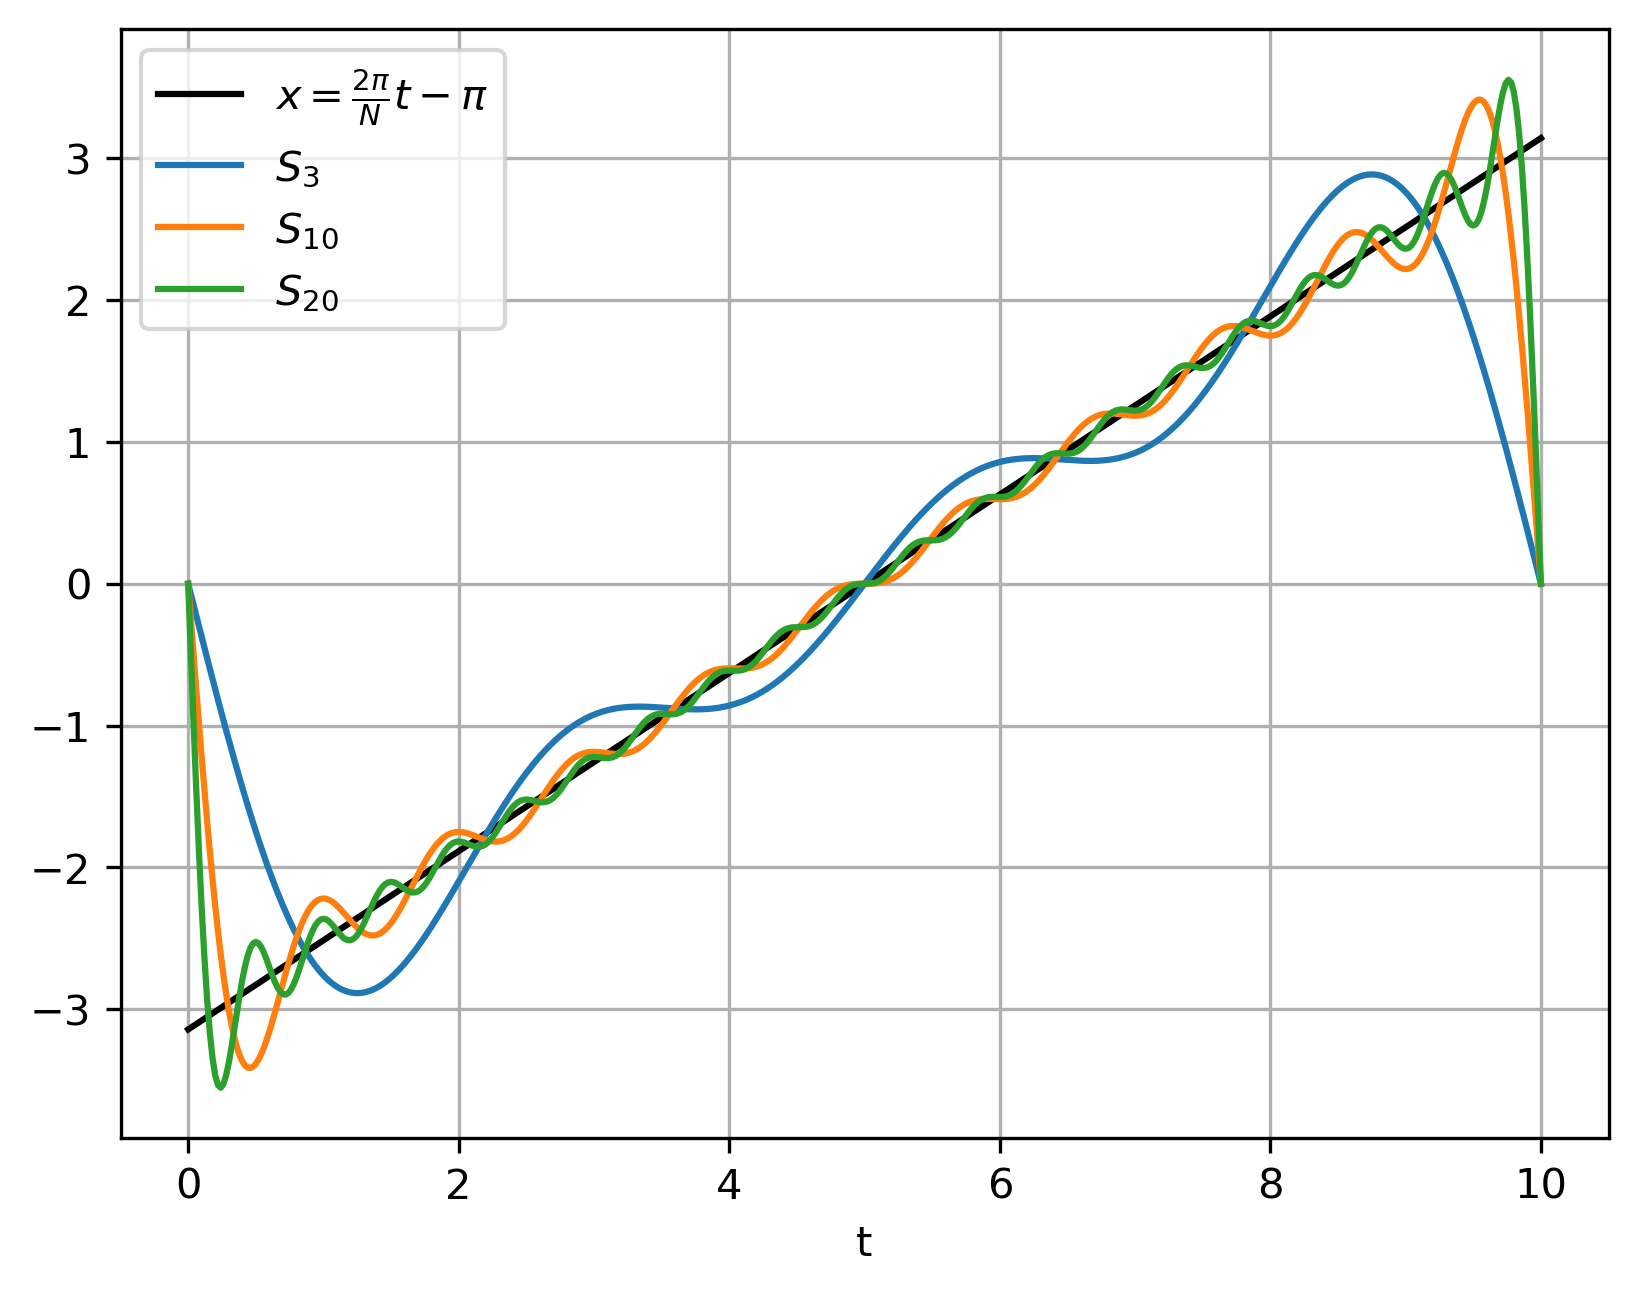
\includegraphics[scale=0.55]{graphics/fourierxapprox.png}\\
Eventually, as $p \to \infty$ and the expression tends to the full Fourier series, $S_p(t)$ will converge to $f(t)$ in the $L^2$ sense\footnote{This is also called \textit{convergence in mean} and is different from \textit{pointwise convergence} that is more intuitive for most people. The rigorous treatment to this requires Measure Theory, and again, Functional Analysis and will not be pursued here.}, with respect to the inner product of Equation (\ref{eqn:integralinner}). This is derived heuristically below.
\begin{align*}
&\quad \lim_{p \to \infty} \norm{f(t) - S_p(t)}^2 = \lim_{p \to \infty} \left(\int_{0}^{N} \abs{f(t) - S_p(t)}^2 dt\right) \\ 
&= \lim_{p \to \infty} \langle f(t) - S_p(t), f(t) - S_p(t) \rangle \\
&= \lim_{p \to \infty} \langle (\lim_{p \to \infty} S_p(t)) - S_p(t)), (\lim_{p \to \infty} S_p(t)) - S_p(t)) \rangle \\
& \quad \text{((d) of Theorem \ref{thm:spectralinner})}\\
&= \lim_{p \to \infty} \begin{aligned}
\left\langle \sum_{k=p+1}^{\infty} [a_k \cos(\frac{2k\pi}{N}t) + b_k \sin(\frac{2k\pi}{N}t)], \right. \\
\left. \sum_{k=p+1}^{\infty} [a_k \cos(\frac{2k\pi}{N}t) + b_k \sin(\frac{2k\pi}{N}t)] \right\rangle \end{aligned} \\
&= \lim_{p \to \infty} \sum_{k=p+1}^{\infty} \frac{N}{2} (a_k^2 + b_k^2) \quad 
\text{(Orthogonality within the Fourier basis)} \\
&= 0
\end{align*}
Notice that the last step requires crucially that the series $\{a_k^2 + b_k^2\}$, $k = p+1, \ldots, \infty$ will converge to zero eventually, i.e.\ $a_k, b_k \to 0$ as $k \to \infty$. This will be justified when we introduce the Parseval's Theorem later on. \par
Returning back to practices in Earth Science, and other fields like Engineering, often we are not given a function that has a closed form to work with. Instead, we collect data from measurements at a fixed sampling rate, and what we obtain is a \textit{discrete time series}. However, we can still try to apply the idea of Fourier, and try to approximate and interpolate the finite time series with sinusoidal functions. Assume that, we have $N$ data points collected for the time series $f(t)$, evenly spaced at time $t = 0, 1, 2, \cdots, N-1$. Further assume that we only use a few of sines and cosines for the approximation, such that the degree $p$ much is less than the number of data points $N$, specifically, $2p+1 \leq N$. The suitable Fourier approximation then will be in the form of Equation (\ref{eqn:fourierpart}) where $N$ is the period of the time series. Since we only have finite data points, we cannot carry out the needed integration to compute (\ref{eqn:fouriersca}) and (\ref{eqn:fourierscb}). Nevertheless, we can borrow the idea in the last chapter and do the approximation in the way such that the Fourier partial sum will achieve the least-square error, summed over the sampling points. Subsequently, the system to be optimized will be
\begin{align*}
\footnotesize
\begin{cases}
\begin{aligned} 
C_0 + A_1 \cos(\frac{2\pi}{N}(0)) + A_2 \cos(\frac{2\pi(2)}{N}(0)) + \cdots + A_p \cos(\frac{2\pi p}{N}(0)) \\
+ B_1 \sin(\frac{2\pi}{N}(0)) + B_2 \sin(\frac{2\pi(2)}{N}(0)) + \cdots + B_p \sin(\frac{2\pi p}{N}(0))
\end{aligned} &= f(0) \\
\begin{aligned} 
C_0 + A_1 \cos(\frac{2\pi}{N}(1)) + A_2 \cos(\frac{2\pi(2)}{N}(1)) + \cdots + A_p \cos(\frac{2\pi p}{N}(1)) \\
+ B_1 \sin(\frac{2\pi}{N}(1)) + B_2 \sin(\frac{2\pi(2)}{N}(1)) + \cdots + B_p \sin(\frac{2\pi p}{N}(1))
\end{aligned} &= f(1) \\
\begin{aligned} 
C_0 + A_1 \cos(\frac{2\pi}{N}(2)) + A_2 \cos(\frac{2\pi(2)}{N}(2)) + \cdots + A_p \cos(\frac{2\pi p}{N}(2)) \\
+ B_1 \sin(\frac{2\pi}{N}(2)) + B_2 \sin(\frac{2\pi(2)}{N}(2)) + \cdots + B_p \sin(\frac{2\pi p}{N}(2))
\end{aligned} &= f(2) \\
\vdots \\
\begin{aligned} 
C_0 + A_1 \cos(\frac{2\pi}{N}(N-1)) + A_2 \cos(\frac{2\pi(2)}{N}(N-1)) + \cdots + A_p \cos(\frac{2\pi p}{N}(0)) \\
+ B_1 \sin(\frac{2\pi}{N}(N-1)) + B_2 \sin(\frac{2\pi(2)}{N}(N-1)) + \cdots + B_p \sin(\frac{2\pi p}{N}(N-1))
\end{aligned} &= f(N-1)
\end{cases}
\end{align*} 
where we have replaced the small letters $a_k, b_k$ by capital letters $A_k, B_k$ and $a_0$ by $C_0$. Or in the form of a matrix system, $G\vec{\beta} = \vec{d}$, where
\begin{align*}
G =
\begin{bmatrix}
1 & 1 & 0 & \cdots & 1 & 0 \\
1 & \cos(\frac{2\pi}{N}) & \sin(\frac{2\pi}{N}) & \cdots & \cos(\frac{2\pi p}{N}) & \sin(\frac{2\pi p}{N}) \\
1 & \cos(\frac{2\pi(2)}{N}) & \sin(\frac{2\pi(2)}{N}) & \cdots & \cos(\frac{2\pi p (2)}{N}) & \sin(\frac{2\pi p (2)}{N}) \\
\vdots & \vdots & \vdots & & \vdots & \vdots \\
1 & \cos(\frac{2\pi(n-1)}{N}) & \sin(\frac{2\pi(n-1)}{N}) & \cdots & \cos(\frac{2\pi p(N-1)}{N}) & \sin(\frac{2\pi p(N-1)}{N}) \\
\end{bmatrix}
\end{align*}
is a $N \times (2p+1)$ matrix and
\begin{align*}
&\vec{\beta} = 
\begin{bmatrix}
C_0 \\
A_1 \\
B_1 \\
\vdots \\
A_p \\
B_p
\end{bmatrix}
&\vec{d} = 
\begin{bmatrix}
f(0) \\
f(1) \\
f(2) \\
\vdots \\
f(N-1)
\end{bmatrix}
\end{align*}
are vectors with $2p+1$ and $N$ entries respectively. The least-square method then sets out to find the best-fit parameters $\vec{\beta} = (C_0, A_1, B_1, \cdots, A_p, B_p)^T$ for this system of equations. From Theorem \ref{thm:bestfit}, we know that the best parameters are found by
\begin{align*}
\vec{\beta}_f = (G^TG)^{-1}G^T\vec{d}
\end{align*}
However, we can greatly simplify the expression, by noticing that every column vector of a sine/cosine series is orthogonal to each other. If we write each sine/cosine term as a complex exponential using Euler's formula in Definition \ref{defn:Euler}, then the column vectors of a sine-cosine pair in $G$ with a frequency of $2\pi k/N$, where both $k$ and $N$ are integers, can be expressed by the real and imaginary parts of
\begin{align*}
\left\{\exp(\imath \frac{2\pi k}{N} t)\right\}_{t = 0,1,2,\ldots,N-1}
&= \left\{\cos(\frac{2\pi k}{N} t) + \imath\sin(\frac{2\pi k}{N} t) \right\}_{t = 0,1,2,\ldots,N-1}
\end{align*}
or in the other way around,
\begin{align*}
\left\{\exp(-\imath \frac{2\pi k}{N} t)\right\}_{t = 0,1,2,\ldots,N-1}
&= \left\{\cos(\frac{2\pi k}{N} t) - \imath\sin(\frac{2\pi k}{N} t) \right\}_{t = 0,1,2,\ldots,N-1}
\end{align*}
We now first prove that the two column vectors of a sine-cosine pair that has the same frequency are orthogonal. We take the sum of squares of the first expression, which gives
\begin{align*}
\sum_{t=0}^{N-1} (\exp(\imath \frac{2\pi k}{N} t))^2 &= \sum_{t=0}^{N-1} (\cos(\frac{2\pi k}{N} t) + \imath\sin(\frac{2\pi k}{N} t))^2 \\
\sum_{t=0}^{N-1} \exp(\imath \frac{4\pi k}{N} t) &= \sum_{t=0}^{N-1} (\cos^2(\frac{2\pi k}{N} t) + 2\imath\sin(\frac{2\pi k}{N} t)\cos(\frac{2\pi k}{N} t) - \sin^2(\frac{2\pi k}{N} t))
\end{align*}
Notice that the left hand side is a geometric sequence with a common ratio $r = \exp(\imath 4\pi k/N)$, whose sum is seen to be
\begin{align*}
\frac{1-r^N}{1-r} &= \frac{1 - \exp(\imath 4\pi k)}{1 - \exp(\imath 4\pi k/N)} = 0
\end{align*}
as $\exp(\imath 4\pi k)$ is just $1$. By comparing the real and imaginary parts, we know that
\begin{align}
\sum_{t=0}^{N-1} \cos^2(\frac{2\pi k}{N} t) &= \sum_{t=0}^{N-1} \sin^2(\frac{2\pi k}{N} t) \label{eqn:sumofsincossq} \\
\sum_{t=0}^{N-1} \sin(\frac{2\pi k}{N} t)\cos(\frac{2\pi k}{N} t) &= 0
\end{align}
The second equation shows that the two column vectors representing the sine and cosine waves of the same frequency have a dot product of zero and hence are orthogonal. \par 

Utilizing the complex formulations, we can also prove that column vectors of sine (or cosine) functions with different frequencies are orthogonal as well. Here we prove one of the cases, where the first series is a sine a frequency of $2\pi k/N$, and the second series is also a sine, of a frequency of $2\pi l/N$, where $k \neq l$ are both integers. We start by considering the sum of products between
\begin{align*}
\left\{\exp(\imath \frac{2\pi k}{N} t)\right\}_{t = 0,1,2,\ldots,N-1} = \left\{\cos(\frac{2\pi k}{N} t) + \imath\sin(\frac{2\pi k}{N} t) \right\}_{t = 0,1,2,\ldots,N-1}   
\end{align*}
and
\begin{align*}
\left\{\exp(\imath \frac{2\pi l}{N} t)\right\}_{t = 0,1,2,\ldots,N-1} = \left\{\cos(\frac{2\pi l}{N} t) + \imath\sin(\frac{2\pi l}{N} t) \right\}_{t = 0,1,2,\ldots,N-1}   
\end{align*}
The analysis is similar to the one above. Particularly, the L.H.S. is zero and by considering the real part of the expression on R.H.S., we have
\begin{align}
\sum_{t=0}^{N-1} \cos(\frac{2\pi k}{N} t)\cos(\frac{2\pi l}{N} t) - \sum_{t=0}^{N-1} \sin(\frac{2\pi k}{N} t)\sin(\frac{2\pi l}{N} t) &= 0 \label{eqn:cossinmixed1}
\end{align}
as long as $k + l$ is not the integer multiples of $N$. (why?)\footnote{The sum of complex exponentials on L.H.S. will then become
\begin{align*}
\sum_{t=0}^{N-1} \exp(\imath \frac{2\pi k}{N} t) \exp(\imath \frac{2\pi l}{N} t) &= \sum_{t=0}^{N-1} \exp(\imath \frac{2\pi k}{N} t) \exp(\imath \frac{2\pi (qN - k)}{N} t) \\
&= \sum_{t=0}^{N-1} \exp(\imath 2\pi q t) = \sum_{t=0}^{N-1} 1 = N \neq 0
\end{align*}
and the argument fails.} We can also consider another sum of products between $\left\{\exp(\imath \frac{2\pi k}{N} t)\right\}_{t = 0,1,2,\ldots,N-1}$ and
\begin{align*}
\left[\exp(-\imath \frac{2\pi l}{N} t)\right]_{t = 0,1,2,\cdots,N-1} = \left[\cos(\frac{2\pi l}{N} t) - \imath\sin(\frac{2\pi l}{N} t) \right]_{t = 0,1,2,\cdots,N-1}       
\end{align*}
Again by looking at the real part, this yields another relation as\footnote{Similarly we have the constraint that $k$ and $l$ are not differed by an integer multiple of $N$.}
\begin{align}
\sum_{t=0}^{N-1} \cos(\frac{2\pi k}{N} t)\cos(\frac{2\pi l}{N} t) + \sum_{t=0}^{N-1} \sin(\frac{2\pi k}{N} t)\sin(\frac{2\pi l}{N} t) &= 0 \label{eqn:cossinmixed2}
\end{align}
From the two derived equations (\ref{eqn:cossinmixed1}) and (\ref{eqn:cossinmixed2}), we can hence conclude that
\begin{align*}
\sum_{t=0}^{N-1} \cos(\frac{2\pi k}{N} t)\cos(\frac{2\pi l}{N} t) &= 0 \\
\sum_{t=0}^{N-1} \sin(\frac{2\pi k}{N} t)\sin(\frac{2\pi l}{N} t) &= 0        
\end{align*}
The orthogonality relations can be proven between a sine and cosine of different frequencies as well in a very similar essence. We will now establish the last result, the dot product of any cosine (or sine) column vector with a specific frequency $2\pi k/N$ with itself. We can consider the sum of products between
\begin{align*}
&\left\{\exp(\imath \frac{2\pi k}{N} t)\right\}_{t = 0,1,2,\ldots,N-1} & \text{ and } & &\left\{\exp(-\imath \frac{2\pi k}{N} t)\right\}_{t = 0,1,2,\ldots,N-1}
\end{align*} 
This time, the L.H.S. is not a geometric series, but rather $N$ terms of $1$. The relation is then
\begin{align}
\sum_{t=0}^{N-1} \cos^2(\frac{2\pi k}{N} t) + \sum_{t=0}^{N-1} \sin^2(\frac{2\pi k}{N} t) &= \sum_{t=0}^{N-1} \exp(\imath \frac{2\pi k}{N} t)\exp(-\imath \frac{2\pi k}{N} t) \nonumber \\
&= \sum_{t=0}^{N-1} (1) \nonumber \\
&= N \label{eqn:samefreqcossin}
\end{align}
Actually it can also be observed from the fact that the sum of a sine-cosine square pair is $1$. Not long before, we have arrived at Equation (\ref{eqn:sumofsincossq})
\begin{align*}
\sum_{t=0}^{N-1} \cos^2(\frac{2\pi k}{N} t) &= \sum_{t=0}^{N-1} \sin^2(\frac{2\pi k}{N} t)     
\end{align*}
Solving these two equations (\ref{eqn:sumofsincossq}) and (\ref{eqn:samefreqcossin}) yields
\begin{align}
\sum_{t=0}^{N-1} \cos^2(\frac{2\pi k}{N} t) &= \sum_{t=0}^{N-1} \sin^2(\frac{2\pi k}{n} t) = \frac{N}{2} \label{eqn:sqcossineNhalf}   
\end{align}
Hence the product $G^TG$, where each entry will be the dot product between the series of sines and cosines, will be
\begin{align*}
G^TG =
\begin{bmatrix}
N & 0 & 0 & \cdots \\
0 & \frac{N}{2} & 0 & \\
0 & 0 & \frac{N}{2} & \\
\vdots & & & \ddots
\end{bmatrix}
\end{align*}
and
\begin{align*}
(G^TG)^{-1} = \frac{1}{N}
\begin{bmatrix}
1 & 0 & 0 & \cdots \\
0 & 2 & 0 & \\
0 & 0 & 2 & \\
\vdots & & & \ddots
\end{bmatrix}    
\end{align*}
So the best-fit parameters are
\begin{align*}
\vec{\beta_f} &= (G^TG)^{-1}G^T\vec{d} \\
\begin{bmatrix}
C_0 \\
A_1 \\
B_1 \\
\vdots \\
\end{bmatrix}
&= \frac{1}{N} 
\begin{bmatrix}
1 & 0 & 0 & \cdots \\
0 & 2 & 0 & \\
0 & 0 & 2 & \\
\vdots & & & \ddots
\end{bmatrix} 
\begin{bmatrix}
1 & 1 & 1 & \cdots \\
1 & \cos(\frac{2\pi}{N}) & \cos(\frac{2\pi(2)}{N}) & \\
0 & \sin(\frac{2\pi}{N}) & \sin(\frac{2\pi(2)}{N}) &  \\
\vdots & & & \ddots
\end{bmatrix}
\begin{bmatrix}
f(0)\\
f(1)\\
f(2)\\
\vdots
\end{bmatrix} \\
\begin{bmatrix}
C_0 \\
A_1 \\
B_1 \\
\vdots \\
\end{bmatrix}
&= 
\frac{1}{N}
\begin{bmatrix}
1 & 1 & 1 & \cdots \\
2 & 2\cos(\frac{2\pi}{N}) & 2\cos(\frac{2\pi(2)}{N}) & \\
0 & 2\sin(\frac{2\pi}{N}) & 2\sin(\frac{2\pi(2)}{N}) &  \\
\vdots & & & \ddots
\end{bmatrix}
\begin{bmatrix}
f(0)\\
f(1)\\
f(2)\\
\vdots
\end{bmatrix} 
\end{align*}
Detailed expressions are
\begin{align}
C_0 &= \frac{1}{N}(f(0) + f(1) + f(2) + \cdots + f(N-1)) \nonumber \\
&= \frac{1}{N}\sum_{t=0}^{n-1} f(t) \label{eqn:protoDFTc}  \\
A_k &= \frac{2}{N}(f(0) + f(1)\cos(\frac{2\pi k}{N}) + \cdots + f(N-1)\cos(\frac{2\pi (N-1)k}{N})) \nonumber \\
&= \frac{2}{N}\sum_{t=0}^{N-1} f(t)\cos(\frac{2\pi kt}{N}) \label{eqn:protoDFTa} \\
B_k &= \frac{2}{N}(f(1)\sin(\frac{2\pi k}{N}) + \cdots + f(N-1)\sin(\frac{2\pi (N-1)k}{N})) \nonumber \\
&= \frac{2}{N}\sum_{t=0}^{N-1} f(t)\sin(\frac{2\pi kt}{N}) \label{eqn:protoDFTb}
\end{align}
That makes sense, at least they seem to be. But in the short exercise that follows the example below you will immediately notice there is a big caveat to this prototype.
\begin{exmp}
\label{exmp:ex11.2.1}
Fit the following time-series with the Fourier basis up to order $p=1$, where $f(0) = 4, f(1) = 1, f(2) = 2, f(3) = 3, f(4) = 1$.
\end{exmp}
\begin{solution}
The degree is $p=1$ and means that there are only three components, which are the constant term, and a sine-cosine pair with a frequency of $\frac{2\pi k}{N}$ where $k=1$, $N=5$. The best-fit parameters will be
\begin{align*}
\begin{bmatrix}
C_0 \\
A_1 \\
B_1
\end{bmatrix}
&= 
\frac{1}{5}
\begin{bmatrix}
1 & 1 & 1 & 1 & 1 \\
2 & 2\cos(\frac{2\pi}{5}) & 2\cos(\frac{2\pi(2)}{5}) & 2\cos(\frac{2\pi(3)}{5}) & 2\cos(\frac{2\pi(4)}{5}) \\
0 & 2\sin(\frac{2\pi}{5}) & 2\sin(\frac{2\pi(2)}{5}) & 2\sin(\frac{2\pi(3)}{5}) & 2\sin(\frac{2\pi(4)}{5})
\end{bmatrix}
\begin{bmatrix}
f(0)\\
f(1)\\
f(2)\\
f(3)\\
f(4)
\end{bmatrix} 
\end{align*}
\begin{align*}
C_0 &= \frac{1}{5} (4+1+2+3+1) = \frac{11}{5} \\
A_1 &= \frac{2}{5} (4 + 1\cos(\frac{2\pi}{5}) + 2\cos(\frac{2\pi(2)}{5}) + 3\cos(\frac{2\pi(3)}{5}) + 1\cos(\frac{2\pi(4)}{5})) \\
&\approx 0.229 \\
B_1 &= \frac{2}{5} (0 + 1\sin(\frac{2\pi}{5}) + 2\sin(\frac{2\pi(2)}{5}) + 3\sin(\frac{2\pi(3)}{5}) + 1\sin(\frac{2\pi(4)}{5})) \\
&\approx -0.235
\end{align*}
So the best trigonometric fit of order $p=1$ for the time-series concerned is
\begin{align*}
f(t) = \frac{11}{5} + 0.229 \cos(\frac{2\pi}{5}t) - 0.235 \sin(\frac{2\pi}{5}t)
\end{align*}
\end{solution}
Short Exercise: Find an improved approximation with order $p = 2$. What happens if $p = 3$? \footnote{For $p = 2$, the best-fit coefficients are
\begin{align*}
\begin{bmatrix}
C_0 \\
A_1 \\
B_1 \\
A_2 \\
B_2
\end{bmatrix}
&= 
\frac{1}{5}
\begin{bmatrix}
1 & 1 & 1 & 1 & 1 \\
2 & 2\cos(\frac{2\pi}{5}) & 2\cos(\frac{2\pi(2)}{5}) & 2\cos(\frac{2\pi(3)}{5}) & 2\cos(\frac{2\pi(4)}{5}) \\
0 & 2\sin(\frac{2\pi}{5}) & 2\sin(\frac{2\pi(2)}{5}) & 2\sin(\frac{2\pi(3)}{5}) & 2\sin(\frac{2\pi(4)}{5}) \\
2 & 2\cos(\frac{2\pi(2)}{5}) & 2\cos(\frac{2\pi(2)(2)}{5}) & 2\cos(\frac{2\pi(2)(3)}{5}) & 2\cos(\frac{2\pi(2)(4)}{5}) \\
0 & 2\sin(\frac{2\pi(2)}{5}) & 2\sin(\frac{2\pi(2)(2)}{5}) & 2\sin(\frac{2\pi(2)(3)}{5}) & 2\sin(\frac{2\pi(2)(4)}{5})
\end{bmatrix}
\begin{bmatrix}
f(0)\\
f(1)\\
f(2)\\
f(3)\\
f(4)
\end{bmatrix}     
\end{align*}
It is not hard to see that $C_0, A_1, B_1$ will be the same and
\begin{align*}
A_2 &= \frac{2}{5} (4 + 1\cos(\frac{2\pi(2)}{5}) + 2\cos(\frac{2\pi(2)(2)}{5}) + 3\cos(\frac{2\pi(2)(3)}{5}) + 1\cos(\frac{2\pi(2)(4)}{5})) \\
&\approx 1.571 \\
B_2 &= \frac{2}{5} (0 + 1\sin(\frac{2\pi(2)}{5}) + 2\sin(\frac{2\pi(2)(2)}{5}) + 3\sin(\frac{2\pi(2)(3)}{5}) + 1\sin(\frac{2\pi(2)(4)}{5})) \\
&\approx 0.380
\end{align*}
Hence the new approximation will be $f(t) = \frac{11}{5} + 0.229 \cos(\frac{2\pi}{5}t) - 0.235 \sin(\frac{2\pi}{5}t) + 1.571 \cos(\frac{2\pi(2)}{5}t) + 0.380 \sin(\frac{2\pi(2)}{5}t)$. When $p$ is increased to $3$, the matrix $G$ involved in the best-fit formula becomes
\begin{align*}
\scriptsize
G = 
\begin{bmatrix}
1 & 1 & 0 & 1 & 0 & 1 & 0 \\
1 & \cos(\frac{2\pi}{5}) & \sin(\frac{2\pi}{5}) & \cos(\frac{2\pi(2)}{5}) & \sin(\frac{2\pi(2)}{5}) & \cos(\frac{2\pi(3)}{5}) & \sin(\frac{2\pi(3)}{5})\\
1 & \cos(\frac{2\pi(2)}{5}) & \sin(\frac{2\pi(2)}{5}) & \cos(\frac{2\pi(2)(2)}{5}) & \sin(\frac{2\pi(2)(2)}{5}) & \cos(\frac{2\pi(3)(2)}{5}) & \sin(\frac{2\pi(3)(2)}{5}) \\
1 & \cos(\frac{2\pi(3)}{5}) & \sin(\frac{2\pi(3)}{5}) & \cos(\frac{2\pi(2)(3)}{5}) & \sin(\frac{2\pi(2)(3)}{5}) & \cos(\frac{2\pi(3)(3)}{5}) & \sin(\frac{2\pi(3)(3)}{5})\\
1 & \cos(\frac{2\pi(4)}{5}) & \sin(\frac{2\pi(4)}{5}) & \cos(\frac{2\pi(2)(4)}{5}) & \sin(\frac{2\pi(2)(4)}{5}) & \cos(\frac{2\pi(3)(4)}{5}) & \sin(\frac{2\pi(3)(4)}{5})
\end{bmatrix}    
\end{align*}
and a routine computation will show that
\begin{align*}
G^T G = 
\begin{bmatrix}
5 & 0 & 0 & 0 & 0 & 0 & 0 \\
0 & \frac{5}{2} & 0 & 0 & 0 & 0 & 0 \\
0 & 0 & \frac{5}{2} & 0 & 0 & 0 & 0 \\
0 & 0 & 0 & \frac{5}{2} & 0 & \frac{5}{2} & 0 \\
0 & 0 & 0 & 0 & \frac{5}{2} & 0 & -\frac{5}{2} \\
0 & 0 & 0 & \frac{5}{2} & 0 & \frac{5}{2} & 0 \\
0 & 0 & 0 & 0 & -\frac{5}{2} & 0 & \frac{5}{2} \\
\end{bmatrix}
\end{align*}
which is not invertible (the fourth/sixth rows are equal and the fifth/last rows are the negative of each other), so that the formula $\vec{\beta}_f = (G^TG)^{-1}G^T\vec{d}$ will fail. If we forcefully use the expressions in (\ref{eqn:protoDFTa}) and (\ref{eqn:protoDFTb}) to compute $A_3$ and $B_3$ we will get
\begin{align*}
A_3 &= \frac{2}{5} (4 + 1\cos(\frac{2\pi(3)}{5}) + 2\cos(\frac{2\pi(3)(2)}{5}) + 3\cos(\frac{2\pi(3)(3)}{5}) + 1\cos(\frac{2\pi(3)(4)}{5})) \\
&= A_2 \\
B_3 &= \frac{2}{5} (0 + 1\sin(\frac{2\pi(3)}{5}) + 2\sin(\frac{2\pi(3)(2)}{5}) + 3\sin(\frac{2\pi(3)(3)}{5}) + 1\sin(\frac{2\pi(3)(4)}{5})) \\
&= -B_2    
\end{align*}
So $A_2$ ($B_2$) and $A_3$ ($B_3$) carry the same information and one of them will be redundant.
}

\subsection{Nyquist Frequency and Real DFT}

While we may want to make the approximation by the Fourier basis as good as possible, we have to know how high the order $p$ needs to be. On the other hand, as we can see in the last example, if $p$ is set too large, the best-fit formula will become problematic and the approximation will contain duplicated terms, in the sense that they take equal values (or with an opposite sign) at all sampling points. For example, if $k + l = N$, then for the integer time steps $t = 0, 1, \ldots, N-1$
\begin{align*}
\cos(\frac{2\pi l}{N} t) &= \cos(\frac{2\pi (N-k)}{N} t) \\
&= \cos(2\pi t - \frac{2\pi k}{N} t) \\
&= \cos(\frac{2\pi k}{N} t)
\end{align*}
so the two cosine waves, despite having different frequencies, coincide at every data point and will be indistinguishable from the time-series. The same problem arises similarly for the sine terms. The condition $k + l = N$ above hints that the maximum value of $p$ should be $N/2$. This corresponds to an angular frequency of $\omega_{\text{Ny}} = \frac{2\pi}{N}(\frac{N}{2}) = \pi$, which is known as the \index{Nyquist Frequency}\keywordhl{Nyquist frequency}. Consequentially, we have the \index{Nyquist Sampling Theorem}\keywordhl{Nyquist Sampling Theorem} as follows.
\begin{thm}[Nyquist Sampling Theorem]
\label{thm:Nyquist}
For an evenly spaced time-series that has a time step of $\Delta t = 1$, any sinuosidal wave with an angular freqency exceeding the Nyquist frequency $\omega > \omega_{\text{Ny}} = \pi$ cannot be properly detected. 
\end{thm}
So it means that the highest resolvable frequency in the time-series is the Nyquist frequency $\omega_{\text{Ny}} = \pi$, or in other words, the minimum period length has to cover at least two time steps. As a result, we only need the sine/cosine terms up to the order $\lfloor N/2 \rfloor$. We have just shown a part of the theorem that if $k + l = N$, then the sinusoidal series of a higher order $l = \lfloor N/2 \rfloor + 1, \ldots, N$ will be redundant in the derivation above. We will complete the theorem by verifying that the sine/cosine terms of an order $l = N+1, N+2, \ldots$ beyond will also lead to duplicated modes: let $l = k + qN$ where $q$ is a positive integer, then
\begin{align*}
\cos(\frac{2\pi l}{N} t) &= \cos(\frac{2\pi (k + qN)}{N} t) \\
&= \cos(\frac{2\pi k}{N} t + 2\pi q t) \\
&= \cos(\frac{2\pi k}{N} t)
\end{align*}
for all time steps $t = 0,1,\ldots,N-1$. Again, it is similar for the sines. Another perspective to see the problem is that, if the "ground truth" function to be approximated by DFT indeed contains some sinusoidal component with a frequency higher than the Nyquist frequency, then its signal will "spill" into a corresponding lower frequency. Again, using cosine and the case $k + l = N$ as an illustration, if $k$ represents the lower frequency mode and $l$ represents the higher one (assumed to have a coefficient of $a_l$), then (\ref{eqn:protoDFTa}) will yield
\begin{align*}
A_k &= \frac{2}{N}\sum_{t=0}^{N-1} (a_l\cos(\frac{2\pi lt}{N})) \cos(\frac{2\pi kt}{N}) \\
&= \frac{2}{N}\sum_{t=0}^{N-1} a_l\cos(\frac{2\pi (N-k)t}{N}) \cos(\frac{2\pi kt}{N}) \\
&= \frac{2}{N}\sum_{t=0}^{N-1} a_l\cos(2\pi t - \frac{2\pi k}{N} t) \cos(\frac{2\pi kt}{N}) \\
&= \frac{2}{N}\sum_{t=0}^{N-1} a_l\cos(\frac{2\pi k}{N} t)) \cos(\frac{2\pi kt}{N}) \\
&= \frac{2}{N}\sum_{t=0}^{N-1} a_l \cos^2(\frac{2\pi kt}{N}) \\
&= \frac{2}{N} (a_l (\frac{N}{2})) = a_l & \text{(Equation (\ref{eqn:sqcossineNhalf}))} 
\end{align*}
Hence any signal with a frequency higher than the Nyquist frequency will contribute to the respective DFT frequency and contaminate it.\par

Now we can formally derive the \index{Real Discrete Fourier Transform}\keywordhl{(real) Discrete Fourier Transform} for a time-series which is given by (\ref{eqn:protoDFTc}), (\ref{eqn:protoDFTa}), and (\ref{eqn:protoDFTb}). In the last part, we have already worked with an odd $N$ (see Example \ref{exmp:ex11.2.1}) where the maximum resolvable degree will be $p = \frac{N}{2} - 1$. When $N$ is even, then we have frequencies from zero to $k = N/2$. Notice that the constant term of zero frequency contributes a single parameter, every other frequency contribute two coefficients via a pair of sine and cosine, and the maximum frequency $k_{\text{Ny}} = N/2$ only give rises to one coefficient from the cosine series which takes the form of alternating $(1,-1,1,-1,\ldots,1,-1)$ (the corresponding diagonal entry in the $(G^TG)^{-1}$ term of the least-square formula will be $1/N$ instead of $2/N$), as the sine function will be always zero at the Nyquist frequency. In both cases, there can be at most $N$ sinusoidal curves for fitting $N$ data points and $G$ will be square. Since the amount of parameters is the same as the number of data, it becomes an interpolation that passes through all the given data points. By convention, we will omit the factor of $1/N$ in the computation of DFT.

\begin{exmp}
Find the Discrete Fourier Transform of the time series $(1,2,1,-1,3,0,2,-2)$.
\end{exmp}
\begin{solution}
According to Theorem \ref{thm:Nyquist}, the highest resolvable degree will be $N/2 = 4$. Its DFT is then given by
\begin{align*}
\scriptsize
\begin{bmatrix}
C_0 \\
A_1 \\
B_1 \\
A_2 \\
B_2 \\
A_3 \\
B_3 \\
A_4
\end{bmatrix}
&= 
\tiny
\begin{bmatrix}
1 & 1 & 1 & 1 & \cdots & 1 & 1 \\
2 & 2\cos(\frac{2\pi}{8}) & 2\cos(\frac{2\pi(2)}{8}) & 2\cos(\frac{2\pi(3)}{8}) & \cdots & 2\cos(\frac{2\pi(6)}{8}) & 2\cos(\frac{2\pi(7)}{8}) \\
0 & 2\sin(\frac{2\pi}{8}) & 2\sin(\frac{2\pi(2)}{8}) & 2\sin(\frac{2\pi(3)}{8}) & \cdots & 2\sin(\frac{2\pi(6)}{8}) & 2\sin(\frac{2\pi(7)}{8}) \\
2 & 2\cos(\frac{2\pi(2)}{8}) & 2\cos(\frac{2\pi(2)(2)}{8}) & 2\cos(\frac{2\pi(2)(3)}{8}) & \cdots & 2\cos(\frac{2\pi(2)(6)}{8}) & 2\cos(\frac{2\pi(2)(7)}{8}) \\
0 & 2\sin(\frac{2\pi(2)}{8}) & 2\sin(\frac{2\pi(2)(2)}{8}) & 2\sin(\frac{2\pi(2)(3)}{8}) & \cdots & 2\sin(\frac{2\pi(2)(6)}{8}) & 2\sin(\frac{2\pi(2)(7)}{8}) \\
2 & 2\cos(\frac{2\pi(3)}{8}) & 2\cos(\frac{2\pi(3)(2)}{8}) & 2\cos(\frac{2\pi(3)(3)}{8}) & \cdots & 2\cos(\frac{2\pi(3)(6)}{8}) & 2\cos(\frac{2\pi(3)(7)}{8}) \\
0 & 2\sin(\frac{2\pi(3)}{8}) & 2\sin(\frac{2\pi(3)(2)}{8}) & 2\sin(\frac{2\pi(3)(3)}{8}) & \cdots & 2\sin(\frac{2\pi(3)(6)}{8}) & 2\sin(\frac{2\pi(3)(7)}{8}) \\
1 & -1 & 1 & -1 & \cdots & 1 & -1
\end{bmatrix}
\scriptsize
\begin{bmatrix}
f(0)\\
f(1)\\
f(2)\\
f(3)\\
f(4)\\
f(5)\\
f(6)\\
f(7)
\end{bmatrix}     
\end{align*}
A direct computation then gives 
\begin{align*}
(C_0, A_1, B_1, A_2, B_2, A_3, B_3, A_4)^T = (6, -2.586, 2.243, 2, 10, -5.414, 6.243, 8)^T
\end{align*}
\end{solution}

\subsection{Complex DFT}

The real DFT approach above has a drawback of using sine-cosine pairs for computation. In Section \ref{section:complexno}, we have learnt the power of complex exponentials to simultaneously represent sines and cosines through Euler's formula, which has also been exploited to derive the relationships between the sinusoidal functions when we are developing the DFT prototype. Therefore, it is incentive to explore the possibility of using complex exponentials to define Discrete Fourier Transform. This has the benefits of simplicity and also convenience when programming.

Continuing from the ideas built in the last section, we propose an interpolation scheme which uses $\exp(i (2\pi k/N) t)$, for a time-series with $N$ data, evenly spaced by a time step of $\Delta t = 1$. The range of $k$ will be from $-\frac{N}{2}, -(\frac{N}{2}-1), \cdots, 0, \frac{N}{2}-1$ for even $N$ and $-\frac{N-1}{2}, -(\frac{N-1}{2}-1), \cdots, 0, \frac{N-1}{2}$ for odd $N$. Both ranges ensure that the total number of complex exponentials used in the fitting process is exactly $N$. Each pair of $k$ and $-k$, i.e.\ $\exp(i (2\pi k/N) t)$ and $\exp(-i (2\pi k/N) t)$ in combination, gives rise to $\cos((2\pi k/N) t)$ and $\sin((2\pi k/N) t)$ by Properties \ref{proper:sincoscomplex}, and so we can expect the correspondence between the real and complex version of Discrete Fourier Transform.\\
\\
Now, the matrix $G$ will take the form of
\begin{align*}
G = \tiny
\left[\begin{array}{@{\,}wc{5pt}wc{40pt}wc{40pt}wc{8pt}wc{56pt}wc{56pt}wc{8pt}wc{40pt}}
1 & 1 & 1 & \cdots & 1 & 1 & \cdots & 1\\
1 & \exp(\imath\frac{2\pi}{N}) & \exp(\imath\frac{2\pi(2)}{N}) & \cdots & \exp(\imath\frac{2\pi(\frac{N}{2}-1)}{N}) & \exp(\imath\frac{2\pi(-\frac{N}{2})}{N}) & \cdots & \exp(-\imath\frac{2\pi}{N}) \\
1 & \exp(\imath\frac{2\pi(2)}{N}) & \exp(\imath\frac{2\pi(2)(2)}{N}) & \cdots & \exp(\imath\frac{2\pi(\frac{N}{2}-1)(2)}{N}) & \exp(\imath\frac{2\pi(-\frac{N}{2})(2)}{N}) & \cdots & \exp(-\imath\frac{2\pi(2)}{N})\\
\vdots & \vdots & & \vdots & \vdots & \vdots &  & \\
1 & \exp(\imath\frac{2\pi(N-1)}{N}) & \exp(\imath\frac{2\pi(2)(N-1)}{N}) & \cdots & \exp(\imath\frac{2\pi(\frac{N}{2}-1)(N-1)}{N}) & \exp(\imath\frac{2\pi(-\frac{N}{2})(N-1)}{N}) & \cdots & \exp(-\imath\frac{2\pi(N-1)}{N}) \\
\end{array}\right]
\end{align*}
for even $N$, where each column representing frequencies that have $k = 0, 1, \cdots, \frac{N}{2}-1, -\frac{N}{2}, \cdots, -1$. This is a common convention where we starts from $k = 0$, and increases to the largest positive $k = \frac{N}{2}-1$, then flips the sign and resumes from the most negative $k = -\frac{N}{2}$, goes all the way back to $k = -1$. For odd $N$, the matrix $G$ is essentially the same, except the $k$ is replaced by the appropriate range of integers and in particular the flipping leads to $k = -\frac{N-1}{2}$. \par
The entries of $G^*G$ in the formula from Theorem \ref{thm:bestfit} are then the complex dot products between the series of complex exponentials appearing as the column vectors of $G$. The orthogonality relation between different column vectors of $G$ is very easy to find. The procedure is similar to what we have done when proving the orthogonality for the real case, but even less tedious. The key point is to write the complex dot product over any pair of two columns as a geometric sequence, that when the values of $k$ are different, will be evaluated to zero. The readers are invited to verify this result, in addition to the fact that the complex dot product between any such a column vector and itself is $N$.\footnote{When $k \neq l$, we have \begin{align*}
\sum_{t=0}^{N-1} \exp(i (2\pi k/N) t)\overline{\exp(i (2\pi l/N) t)} &= \sum_{t=0}^{N-1} \exp(i (2\pi k/N) t)\exp(-i (2\pi l/N) t) \\
&= \sum_{t=0}^{N-1} \exp(i (2\pi (k-l)/N) t) \\
&= \frac{1-\exp(i (2\pi (k-l)/N))^N}{1-\exp(i (2\pi (k-l)/N))} \\
&= \frac{1-\exp(i (2\pi (k-l)))}{1-\exp(i (2\pi (k-l)/N))} \\
&= \frac{1-1}{1-\exp(i (2\pi (k-l)/N))} = 0
\end{align*} If $k = l$, then $\exp(i (2\pi k/N) t)\overline{\exp(i (2\pi l/N) t)} =  \exp(i (2\pi k/N) t)\exp(-i (2\pi k/N) t) = 1$, and the sum will be $N$.} Thus, the expression $G^*G$ is just $N$ times the identity $I$, and $(G^*G)^{-1} = \frac{1}{N} I$. \par
Now we denote the new, complex best-fit parameters, or coefficients by $C_k$. Subsequently,
\begin{align*}
\vec{\beta}_f &= (G^*G)^{-1}G^*\vec{d} = (\frac{1}{N}I)G^*\vec{d} \\
\small
\begin{bmatrix}
C_0 \\
C_1 \\
\vdots \\
C_{N/2-1} \\
C_{-N/2} \\
\vdots \\
C_{-1}
\end{bmatrix}
&= 
\frac{1}{N}
\footnotesize
\begin{bmatrix}
1 & 1 & 1 & \cdots \\
1 & \exp(-\imath\frac{2\pi}{N}) & \exp(-\imath\frac{2\pi(2)}{N}) & \cdots \\
\vdots & \vdots & \vdots & \\
1 & \exp(-\imath\frac{2\pi(N/2-1)}{N}) & \exp(-\imath\frac{2\pi(N/2-1)(2)}{N}) & \cdots \\
1 & \exp(-\imath\frac{2\pi(-N/2)}{N}) & \exp(-\imath\frac{2\pi(-N/2)(2)}{N}) & \cdots \\
\vdots & \vdots & \vdots & \\
1 & \exp(-\imath\frac{2\pi(-1)}{N}) & \exp(-\imath\frac{2\pi(-1)(2)}{N}) & \cdots
\end{bmatrix}
\small
\begin{bmatrix}
f(0) \\
f(1) \\
f(2) \\
\vdots
\end{bmatrix}
\end{align*}
Again this is for even $N$, and we ought to replace the indices for coefficients and complex exponentials appropriately for odd $N$. Again, the $1/N$ factor will be ignored. We now conclude the method of \index{Complex Discrete Fourier Transform}\keywordhl{(complex) Discrete Fourier Transform} in a compact way as follows.
\begin{defn}
\label{defn:complexDFT}
The coefficients, or amplitudes, of the DFT in complex form are computed by
\begin{align*}
C_k = \sum_{t=0}^{N-1} f(t)\exp(-\imath\frac{2\pi k}{N}t)
\end{align*}
where $N$ is the number of data. $k$ are all integers ranging from $[-\frac{N}{2}, \frac{N}{2}-1]$ for even $N$, and $[-\frac{N-1}{2}, \frac{N-1}{2}]$ for odd $N$. For a time step $\Delta t$ different from $1$, the appropriate expression is
\begin{align*}
C_k = \sum_{s=0}^{N-1} f(s\Delta t)\exp(-\imath\frac{2\pi k}{n\Delta t}s)
\end{align*}
We will sometimes denote the series of $C_k$ by $F(k)$ or $\hat{f}(k)$.
\end{defn}
The negative sign inside the complex exponentials in the formula comes from the conjugate transpose required to produce $G^*$. The relation between $C_k$ and the parameters $A_k$, $B_k$ in the real counterpart are inferred from Properties \ref{proper:sincoscomplex} and comparing the expression for the real case\footnote{\begin{align*}
\frac{C_k + C_{-k}}{N} &= \frac{1}{N}\left(\sum_{t=0}^{N-1} f(t)\exp(-\imath\frac{2\pi k}{N}t) + \sum_{t=0}^{N-1} f(t)\exp(-\imath\frac{2\pi (-k)}{N}t)\right) \\ 
&= \frac{1}{N}(\sum_{t=0}^{N-1} f(t)\left(\exp(-\imath\frac{2\pi k}{N}t) + \exp(\imath\frac{2\pi k}{N}t)\right)) \\
&= \frac{2}{N} \sum_{t=0}^{N-1} f(t) \cos(\frac{2\pi k}{N}t) \qquad \text{(Properties \ref{proper:sincoscomplex})}
\end{align*}
which is just equal to $A_k$ in Equation (\ref{eqn:protoDFTa}). The derivation is similar for $B_k$.}, that is
\begin{align*}
A_k &= \frac{C_k + C_{-k}}{N} \\
B_k &= -\frac{(C_k - C_{-k})}{N i}
\end{align*}
for $k \neq 0$. If $N$ is even, then we define $C_N = 0$ for convenience. Moreover, since sine is an odd function, and cosine is an even function, $\Re(C_k) = \Re(C_{-k})$, and $\Im(C_k) = -\Im(C_{-k})$ if the input signal $f(t)$ is real-valued, or in other words, $C_k$ and $C_{-k}$ are a pair of complex conjugates. And so an alternative relationship between the real and complex DFT is
\begin{proper}
\label{proper:FTrealcomplex}
Given a real time-series, the amplitudes $A_k$, $B_k$ in real DFT, and $C_k$ in complex DFT satisfy the relations
\begin{align*}
A_k &= 2\Re(C_k)/N \\
B_k &= -2\Im(C_k)/N
\end{align*}
for any $0 \neq \abs{k} < N$. Meanwhile, $C_0$ is the same in both types of DFT and when $N$ is even, $A_N$ = $C_N/N$. The $1/N$ factor is optional and depends on if any convention is used.
\end{proper}

\begin{exmp}
\label{exmp:ex11.2.2}
Find the complex DFT for the time-series in example \ref{exmp:ex11.2.1}.
\end{exmp}
\begin{solution}
Using the formula in Definition \ref{defn:complexDFT}, we have
\begin{align*}
C_0 &= 4+1+2+3+1 = 11 \\
C_1 &= 4 + 1\exp(-i\frac{2\pi}{5}) + 2\exp(-i\frac{2\pi(2)}{5}) + \\
&\quad 3\exp(-i\frac{2\pi(3)}{5}) + 1\exp(-i\frac{2\pi(4)}{5}) = 0.573 + 0.588i \\
C_2 &= 4 + 1\exp(-i\frac{2\pi(2)}{5}) + 2\exp(-i\frac{2\pi(2)(2)}{5}) \\
&\quad+ 3\exp(-i\frac{2\pi(2)(3)}{5}) + 1\exp(-i\frac{2\pi(2)(4)}{5}) = 3.927 - 0.951i
\end{align*}
Either by the aforementioned property or a direct computation, $C_{-1}$ and $C_{-2}$ are seen to be the complex conjugates of $C_1$ and $C_2$ respectively. 
\end{solution}
Short Exercise: Check if Properties \ref{proper:FTrealcomplex} is true in this example.\footnote{We will only check $A_1$ and $B_1$ and leave $A_2$ and $B_2$ to the readers. $2\Re(C_1)/N = 2(0.573)/5 \approx 0.229 = A_1$, $-2\Im(C_1)/N = -2(0.588)/5 \approx -0.235 = B_1$.}

\subsection{Inverse DFT}

During the derivation of complex DFT, we have found that $G^*G = I$ (omitting the factor $N$) and thus the square matrix $G$ is unitary by Definition \ref{defn:unitary}. This further implies that $G^* = G^{-1}$ (and thus $(G^*)^{-1} = G$) is invertible. And since the complex DFT coefficients are given by $C_k = G^*\vec{d}$, we can undo the DFT and recover the original time-series by multiplying to the left with the inverse $(G^*)^{-1}$ so that $\vec{d} = (G^*)^{-1}C_k = G C_k$. This means that
\begin{align*}
\scriptsize
\begin{bmatrix}
f(0) \\
f(1) \\
f(2) \\
\vdots
\end{bmatrix}    
&= 
\frac{1}{N}
\tiny
\left[\begin{array}{@{\,}wc{6pt}wc{36pt}wc{10pt}wc{52pt}wc{52pt}wc{10pt}wc{36pt}}
1 & 1 & \cdots & 1 & 1 & \cdots & 1 \\
1 & \exp(\imath\frac{2\pi}{N}) & \cdots & \exp(\imath\frac{2\pi(N/2-1)}{N}) & \exp(\imath\frac{2\pi(-N/2)}{N}) & \cdots & \exp(\imath\frac{2\pi(-1)}{N}) \\
1 & \exp(\imath\frac{2\pi(2)}{N}) & \cdots & \exp(\imath\frac{2\pi(N/2-1)(2)}{N}) & \exp(\imath\frac{2\pi(-N/2)(2)}{N}) & \cdots & \exp(\imath\frac{2\pi(-1)(2)}{N}) \\
\vdots & \vdots &  & \vdots & \vdots & & \vdots \\
\end{array}\right]
\scriptsize
\begin{bmatrix}
C_0 \\
C_1 \\
\vdots \\
C_{N/2-1} \\
C_{-N/2} \\
\vdots \\
C_{-1}
\end{bmatrix}
\end{align*}
for even $N$, and can be adapted for odd $N$ with small tweaks similar to those before. It can also be written in a summation form just like the one in Definition \ref{defn:complexDFT} as below.
\begin{defn}
\label{defn:iDFT}
The inverse Discrete Fourier Transform is computed by
\begin{align*}
f(t) &= \frac{1}{N}\sum_{k= -\lfloor \frac{N}{2} \rfloor}^{\lfloor \frac{N-1}{2} \rfloor} F(k)\exp(\imath\frac{2\pi k}{N}t)
\end{align*}
Sometimes we use the operator symbol $F^{-1}$ to denote the inverse DFT operation.
\end{defn}
This can also be verified by a direct substitution. Plugging in the formula from Definition \ref{defn:complexDFT} (with a dummy variable $t'$) into R.H.S., we have
\begin{align*}
&\quad \frac{1}{N}\sum_{k= -\lfloor \frac{N}{2} \rfloor}^{\lfloor \frac{N-1}{2} \rfloor} \left(\sum_{t'=0}^{N-1} f(t')\exp(-\imath\frac{2\pi k}{N}t')\right) \exp(\imath\frac{2\pi k}{n}t) \\
&= \frac{1}{N} \sum_{t'=0}^{N-1} f(t') \left(\sum_{k= -\lfloor \frac{N}{2} \rfloor}^{\lfloor \frac{N-1}{2} \rfloor} \exp(\imath\frac{2\pi k}{N}(t-t'))\right)
\end{align*}
where
\begin{align}
\sum_{k= -\lfloor \frac{N}{2} \rfloor}^{\lfloor \frac{N-1}{2} \rfloor} \exp(\imath\frac{2\pi k}{N}(t-t')) = 
\begin{cases}
N & \text{if $t = t'$} \\
0 & \text{if $t \neq t'$}
\end{cases} \label{eqn:DFTdoublesum}
\end{align}
The first case should be obvious, while the second case is derived in the footnote.\footnote{
For an integer $t - t' = \Delta t \neq 0$, we have
\begin{align*}
\sum_{k= -\lfloor \frac{N}{2} \rfloor}^{\lfloor \frac{N-1}{2} \rfloor} \exp(\imath\frac{2\pi k}{N}\Delta t) 
&= \exp(\imath\frac{2\pi (-\lfloor \frac{N}{2} \rfloor)}{N}(\Delta t)) \frac{1 - \exp(\imath\frac{2\pi \Delta t}{N})^N}{1 - \exp(\imath\frac{2\pi \Delta t}{N})} \\
&= \exp(\imath\frac{-2\pi \lfloor \frac{N}{2} \rfloor}{N}(\Delta t)) \frac{1 - \exp(\imath 2\pi \Delta t)}{1 - \exp(\imath\frac{2\pi \Delta t}{N})} \\
&= \exp(\imath\frac{-2\pi \lfloor \frac{N}{2} \rfloor)}{N}(\Delta t)) \frac{1 - 1}{1 - \exp(\imath\frac{2\pi \Delta t}{N})} = 0
\end{align*}
as a geometric sum that evaluates to zero. $\Delta t$ cannot be an integer multiple of $N$ as well but the range of summation prevents this.} Hence
\begin{align*}
\frac{1}{N} \sum_{t'=0}^{N-1} f(t') \left(\sum_{k= -\lfloor \frac{N}{2} \rfloor}^{\lfloor \frac{N-1}{2} \rfloor} \exp(\imath\frac{2\pi k}{N}(t-t'))\right) &= \frac{1}{N} ((0) + \cdots + f(t) (N) + \cdots + (0)) \\
&= f(t)   
\end{align*}
so the R.H.S. indeed reproduces the original function on L.H.S.

\begin{exmp}
Apply the inverse DFT on $C_{-3} = 1, C_{-2} = 1 + i, C_{-1} = 2 - i, C_0 = 3, C_1 = 2 + i, C_2 = 1 - i$ to retrieve the physical time-series.
\end{exmp}
\begin{solution}
The time series $f(t)$ will have a period of $6$ where $t = 0,1,2,3,4,5$. By Definition \ref{defn:iDFT}, we have
\begin{align*}
f(0) &= \frac{1}{N}\sum_{k=-3}^{2} F(k)\exp(i\frac{2\pi k}{N}(0)) \\
&= \frac{1}{6}[C_{-3}\exp(i\frac{2\pi (-3)}{6}(0)) + C_{-2}\exp(i\frac{2\pi (-2)}{6}(0)) \\
&\quad + C_{-1}\exp(i\frac{2\pi (-1)}{6}(0)) + C_{0}\exp(i\frac{2\pi (0)}{6}(0)) \\
&\quad + C_{1}\exp(i\frac{2\pi (1)}{6}(0)) + C_{2}\exp(i\frac{2\pi (2)}{6}(0))] \\
&= \frac{1}{6}[(1) + (1+i) + (2-i) + 3 + (2+i) + (1-i)] = \frac{10}{6} \\
f(1) &= \frac{1}{N}\sum_{k=-3}^{2} F(k)\exp(i\frac{2\pi k}{N}(1)) \\
&= \frac{1}{6}[C_{-3}\exp(i\frac{2\pi (-3)}{6}(1)) + C_{-2}\exp(i\frac{2\pi (-2)}{6}(1)) \\
&\quad + C_{-1}\exp(i\frac{2\pi (-1)}{6}(1)) + C_{0}\exp(i\frac{2\pi (0)}{6}(1)) \\
&\quad + C_{1}\exp(i\frac{2\pi (1)}{6}(1)) + C_{2}\exp(i\frac{2\pi (2)}{6}(1))] \\
&= \frac{1}{6}[(1)(-1) + (1+i)e^{-i \frac{2\pi}{3}} + (2-i)e^{-i \frac{\pi}{3}} + 3 + (2+i)e^{i \frac{\pi}{3}} + (1-i)e^{i \frac{2\pi}{3}}] \\
&= \frac{1}{2} \\
f(2) &= \frac{1}{N}\sum_{k=-3}^{2} F(k)\exp(i\frac{2\pi k}{N}(2)) \\
&= \frac{1}{6}[C_{-3}\exp(i\frac{2\pi (-3)}{6}(2)) + C_{-2}\exp(i\frac{2\pi (-2)}{6}(2)) \\
&\quad + C_{-1}\exp(i\frac{2\pi (-1)}{6}(2)) + C_{0}\exp(i\frac{2\pi (0)}{6}(2)) \\
&\quad + C_{1}\exp(i\frac{2\pi (1)}{6}(2)) + C_{2}\exp(i\frac{2\pi (2)}{6}(2))] \\
&= \frac{1}{6}[(1)(1) + (1+i)e^{-i \frac{4\pi}{3}} + (2-i)e^{-i \frac{2\pi}{3}} + 3 + (2+i)e^{i \frac{2\pi}{3}} + (1-i)e^{i \frac{4\pi}{3}}] \\
&\approx 0.4107 
\end{align*}
We leave the calculations for the remaining three data points to the readers. They are $f(3) = 0$, $f(4) \approx 0.7440$, and $f(5) = \frac{1}{2}$.
\end{solution}

\section{Properties of DFT}

\subsection{Power Spectrum and Parseval’s Theorem}

The complex DFT coefficients actually store the relevant information of sinusoidal signals in the corresponding frequencies, namely the \textit{phase} and \textit{amplitude}. To see this, go back to Properties \ref{proper:FTrealcomplex}, where
\begin{align*}
A_k &= 2\Re(C_k)/N \\
B_k &= -2\Im(C_k)/N 
\end{align*}
but also, the wave signal of that particular frequency takes the form of
\begin{align*}
A_k \cos(\frac{2\pi k}{N}t) + B_k \sin(\frac{2\pi k}{N}t)
\end{align*}
Plugging in gives
\begin{align*}
&\quad \frac{2}{N} (\Re(C_k)\cos(\frac{2\pi k}{N}t) - \Im(C_k) \sin(\frac{2\pi k}{N}t)) \\
&= \frac{2}{N} (\hat{A}_k \cos \phi_k \cos(\frac{2\pi k}{N}t) - \hat{A}_k\sin\phi_k \sin(\frac{2\pi k}{N}t)) \\
&= \frac{2}{N} \hat{A}_k \cos(\frac{2\pi k}{N}t + \phi_k)
\end{align*}
where we let $-\pi \leq \phi_k < \pi$ and $\hat{A}_k \geq 0$ as real-valued quantities, in a way such that $\Re(C_k) = \hat{A}_k \cos \phi_k$ and $\Im(C_k) = \hat{A}_k \sin \phi_k$, and then apply the trigonometric identity $\cos(\alpha + \beta) = \cos\alpha \cos\beta - \sin\alpha \sin\beta$. $\phi_k$ and $\hat{A}_k$ will be the phase (relative to a cosine wave) and the amplitude of the signal (again putting the $\frac{2}{N}$ factor aside) at the $k$-th frequency respectively. The required values of $\phi_k$ and $\hat{A}_k$ are then derived according to
\begin{align*}
\frac{\Re(C_k)}{\Im(C_k)} &= \frac{\sin \phi_k}{\cos \phi_k} = \tan \phi_k \\
\Re(C_k)^2 + \Im(C_k)^2 &= \hat{A}_k^2 \cos^2 \phi_k + \hat{A}_k^2 \sin^2 \phi_k = \hat{A}_k^2 
\end{align*}
Thus $\phi_k = \arctan(\frac{\Im(C_k)}{\Re(C_k)})$ and $\hat{A}_k = \sqrt{\Re(C_k)^2 + \Im(C_k)^2}$. Recall that from Section \ref{section:complexnogeo} these are exactly the argument and modulus of $C_k$. Therefore, by simply looking at the complex DFT coefficient $C_k$ we can readily extract the phase and amplitude of the corresponding DFT signal. However, in the area of signal processing, we often report the \textit{power} of the signal instead of its amplitude for convenience, which is just the square of the amplitude. It can be easily obtained from
\begin{align*}
\abs{C_k}^2 = C_k\overline{C_k} = C_kC_{-k}
\end{align*}
due to Equation (\ref{eqn:zzbar}) and the fact that $C_k$ has $C_{-k}$ as its complex conjugate (if the input time-series is real-valued). The powers over all frequencies are collectively referred to as the \index{Power Spectrum}\keywordhl{power spectrum}.

\begin{exmp}
Find the phase and power at each frequency bin for the complex DFT computed in Example \ref{exmp:ex11.2.2}.   
\end{exmp}
\begin{solution}
The phase of the zeroth frequency (i.e. constant term) signal is trivially zero, and its power is simply $C_0^2 = (11)^2 = 121$. For the first (base) frequency, the phase is
\begin{align*}
\phi_1 = \arctan(\frac{\Im(C_1)}{\Re(C_1)}) = \arctan(\frac{0.588}{0.573}) = \SI{0.80}{\radian}
\end{align*}
and the power is
\begin{align*}
\abs{C_1}^2 = \abs{C_{-1}}^2 = C_1C_{-1} &= (0.573 + 0.588i)(0.573 - 0.588i) \\
&= 0.67
\end{align*}
Similar for the second frequency, the phase is
\begin{align*}
\phi_2 = \arctan(\frac{\Im(C_2)}{\Re(C_2)}) = \arctan(\frac{-0.951}{3.927}) = \SI{-0.24}{\radian}
\end{align*}
and the power is
\begin{align*}
\abs{C_2}^2 = \abs{C_{-2}}^2 = C_2C_{-2} &= (3.927 - 0.951i)(3.927 + 0.951i) \\
&= 16.33
\end{align*}
\end{solution}
The full power spectrum across all frequencies are related to the initial time-series according to the \keywordhl{Parseval's Theorem}.
\begin{thm}[Parseval's Theorem]
\label{thm:DFTParseval}
The sum of powers for each DFT coefficients divided by the length $N$ is equal to the sum of all data values in the (real) time-series squared, i.e.\
\begin{align*}
\sum_{t=0}^{N-1} f(t)^2 &= \frac{1}{N} \sum_{k= -\lfloor \frac{N}{2} \rfloor}^{\lfloor \frac{N-1}{2} \rfloor} \abs{F(k)}^2
\end{align*}
\end{thm}
\begin{proof}
By substituting the form of inverse DFT given in Definition \ref{defn:iDFT}, the L.H.S. becomes 
\begin{align*}
\sum_{t=0}^{N-1} f(t)^2 &= \sum_{t=0}^{N-1} \left[ \frac{1}{N} \sum_{k= -\lfloor \frac{N}{2} \rfloor}^{\lfloor \frac{N-1}{2} \rfloor} F(k)\exp(\imath\frac{2\pi k}{N}t) \left( \overline{ \frac{1}{N}\sum_{l= -\lfloor \frac{N}{2} \rfloor}^{\lfloor \frac{N-1}{2} \rfloor} F(l)\exp(\imath\frac{2\pi l}{N}t)} \right) \right] \\
&= \frac{1}{N^2} \sum_{k= -\lfloor \frac{N}{2} \rfloor}^{\lfloor \frac{N-1}{2} \rfloor} F(k) \left(\sum_{t=0}^{N-1} \exp(\imath\frac{2\pi k}{N}t) \left( \sum_{l= -\lfloor \frac{N}{2} \rfloor}^{\lfloor \frac{N-1}{2} \rfloor} \overline{F(l)}\exp(-\imath\frac{2\pi l}{N}t) \right) \right) \\
&= \frac{1}{N^2} \sum_{k= -\lfloor \frac{N}{2} \rfloor}^{\lfloor \frac{N-1}{2} \rfloor} F(k) \left( \sum_{l= -\lfloor \frac{N}{2} \rfloor}^{\lfloor \frac{N-1}{2} \rfloor}  \sum_{t=0}^{N-1} \overline{F(l)}\exp(\imath\frac{2\pi (k-l)}{N}t) \right) 
\end{align*}
Similar to (\ref{eqn:DFTdoublesum}), we have
\begin{align*}
\sum_{t=0}^{N-1} \exp(\imath\frac{2\pi (k-l)}{N}t)  = 
\begin{cases}
N & \text{if $k = l$} \\
0 & \text{if $k \neq l$}
\end{cases}     
\end{align*}
Thus
\begin{align*}
&\quad \frac{1}{N^2} \sum_{k= -\lfloor \frac{N}{2} \rfloor}^{\lfloor \frac{N-1}{2} \rfloor} F(k) \left( \sum_{l= -\lfloor \frac{N}{2} \rfloor}^{\lfloor \frac{N-1}{2} \rfloor}  \sum_{t=0}^{N-1} \overline{F(l)}\exp(\imath\frac{2\pi (k-l)}{N}t) \right) \\
&= \frac{1}{N^2} \sum_{k= -\lfloor \frac{N}{2} \rfloor}^{\lfloor \frac{N-1}{2} \rfloor} F(k) [(0) + \cdots + \overline{(F(k))}(N) + \cdots + (0)] \\
&= \frac{1}{N^2} \sum_{k= -\lfloor \frac{N}{2} \rfloor}^{\lfloor \frac{N-1}{2} \rfloor} N F(k)\overline{F(k)} \\
&= \frac{1}{N} \sum_{k= -\lfloor \frac{N}{2} \rfloor}^{\lfloor \frac{N-1}{2} \rfloor} \abs{F(k)}^2
\end{align*} 
is equal to the R.H.S.
\end{proof}

\begin{exmp}
Verify the Parseval's Theorem for Examples \ref{exmp:ex11.2.1} and \ref{exmp:ex11.2.2}.
\end{exmp}
\begin{solution}
The L.H.S. of the formula in Theorem \ref{thm:DFTParseval} applied to the time-series of Example \ref{exmp:ex11.2.1}, is simply
\begin{align*}
\sum_{t=0}^{4} f(t)^2 &= f(0)^2 + f(1)^2 + f(2)^2 + f(3)^2 + f(4)^2 \\
&= (4)^2 + (1)^2 + (2)^2 + (3)^2 + (1)^2 = 31    
\end{align*}
and from Example \ref{exmp:ex11.2.2}, the R.H.S. is
\begin{align*}
\frac{1}{5}\sum_{k=-2}^{2} \abs{F(k)}^2 &= \frac{1}{5}(\abs{C_{-2}}^2 + \abs{C_{-1}}^2 + \abs{C_{0}}^2 + \abs{C_{1}}^2 + \abs{C_{2}}^2) \\
&= \frac{1}{5}(16.33 + 0.67 + 121 + 0.67 + 16.33) \\
&= \frac{1}{5} (155) = 31
\end{align*}
which are indeed equal.
\end{solution}

\subsection{Convolution Theorem}

\index{Convolution}\keywordhl{Convolution} often appears along with Fourier Transform due to an elegant theorem that will be introduced soon. In the area of Earth Science, as well as Physics and Statistics, convolution commonly has a place in describing the solution of problems, e.g.\ via \textit{Green's Function}. Now we are going to introduce how convolution in a discrete sense is defined first, and a daily example will be provided as an illustration. It always involves two time-series or functions.
\begin{defn}[Discrete Convolution]
\label{defn:convolution}
The convolution $h(t)$ between two discrete time-series $f(t)$ and $g(t)$ is written as $f(t) * g(t)$, defined by
\begin{align*}
h(t) = f(t) * g(t) = \sum_{\tau=-\infty}^{\infty} f(\tau) g(t-\tau)
\end{align*}
if $\tau$ takes a value so that the index in either $f$ or $g$ is out of their range, then the term is treated as zero.
\end{defn}
A schematic diagram of convolution is provided as Figure \ref{fig:convschm}. Note that the formula for convolution is symmetric such that we can also define it as $\sum_{\tau=-\infty}^{\infty} f(t-\tau) g(\tau)$. Now, for instance, if $f(t)$ is defined from $t = 0$ and $t = 4$ and $g(t)$ is defined from $t = 0$ and $t = 6$ so that they have a length of $5$ and $7$ respectively, then
\begin{align*}
h(0) &= f(0)g(0) \\
h(1) &= f(0)g(1-0) + f(1)g(1-1) = f(0)g(1) + f(1)g(0) \\
h(4) &= f(0)g(4-0) + f(1)g(4-1) + f(2)g(4-2) \\
&\quad + f(3)g(4-3) + f(4)g(4-4) \\
&= f(0)g(4) + f(1)g(3) + f(2)g(2) + f(3)g(1) + f(4)g(0)
\end{align*}
and
\begin{align*}
h(6) &= f(0)g(6-0) + f(1)g(6-1) + f(2)g(6-2) \\
&\quad + f(3)g(6-3) + f(4)g(6-4) \\
&= f(0)g(6) + f(1)g(5) + f(2)g(4) + f(3)g(3) + f(4)g(2) \\
h(9) &=  f(3)g(6-0) + f(4)g(6-1) = f(3)g(6) + f(4)g(5) \\
h(10) &= f(4)g(6)
\end{align*}
Moreover, $h(t) = 0$ for $t \geq 11$ or $t < 0$ so the effective length of $h(t)$ is $11$. It is not hard to deduce that the resulting convolution will has a length of $m + n - 1$ if the two input time-series have a length of $m$ and $n$.

\begin{exmp}
The probability of Mary getting married within some years can be described by the time-series $q(t)$, where
\begin{align*}
q(t) = 
\begin{cases}
0.2 & 0 \leq t \leq 2 \\
0.1 & 3 \leq t \leq 6 \\
0 & t \geq 7
\end{cases}
\end{align*}
The probability $r(t)$ that Mary gives birth to a baby some years $t$ after marriage is
\begin{align*}
r(t) = 
\begin{cases}
0 & t = 0 \\
0.15 & 1 \leq t \leq 4 \\
0.08 & 5 \leq t \leq 9 \\
0 & t \geq 10
\end{cases}    
\end{align*}
Find the net probability of Mary getting a baby at some years $t$ from now on, assuming she will only get pregnant after married. 
\end{exmp}
\begin{solution}
The required probability $p(t) = q(t) * r(t)$ is actually given by the convolution between $q(t)$ and $r(t)$, which effectively have a length of $7$ and $9$. Particularly, taking $t = 5$ as an example, then we have
\begin{align*}
p(t = 5) &= P(\text{Birth 5 yrs later}|\text{Married now})P(\text{Married now}) \\
&\quad+ P(\text{Birth 4 yrs later}|\text{Married 1 yr later})P(\text{Married 1 yr later})\\
&\quad+ \cdots \\
&\quad+ P(\text{Birth 1 yr later}|\text{Married 4 yrs later})P(\text{Married 4 yrs later}) \\
&\quad+ P(\text{Birth now}|\text{Married 5 yrs later})P(\text{Married 5 yrs later}) \\
&= q(0)r(5) + q(1)r(4) + q(2)r(3) \\
&\quad + q(3)r(2) + q(4)r(1) + q(5)r(0) \\
&= (0.2)(0.08) + (0.2)(0.15) + (0.2)(0.15) \\
&\quad + (0.1)(0.15) + (0.1)(0.15) + (0.1)(0) \\
&= 0.106
\end{align*}
where $P(A|B)$ is the conditional probability of $A$ occurring when $B$ has happened.
\end{solution}
Short Exercise: Find the chance of Mary getting a baby at $8$ years later by convolution.\footnote{It is $q(0)r(8) + q(1)r(7) + q(2)r(6) + q(3)r(5) + q(4)r(4) + q(5)r(3) + q(6)r(2) = (0.2)(0.08) + (0.2)(0.08) + (0.2)(0.08) + (0.1)(0.08) + (0.1)(0.15) + (0.1)(0.15) + (0.1)(0.15) = 0.101$.}\par

\begin{figure}
    \centering
    \begin{tikzpicture}
    \draw[blue, thick] (-3,4+0.5) -- (0,4+0.5) -- (0,6+0.5) -- (2,6+0.5) -- (2,4+0.5) -- (5,4+0.5);
    \node[blue] at (-1,6+0.5) {$f$};
    \draw[red, thick] (-3,0+0.5) -- (0,0+0.5) -- (2,2+0.5) -- (2,0+0.5) -- (5,0+0.5);
    \node[red] at (-1,2+0.5) {$g$};
    \draw[Green, thick] (-3,-4+0.5) -- (-1,-4+0.5) -- plot[domain=-1:1,samples=50] (\x, {0.5*(\x+1)^2 - 4 +0.5}) -- plot[domain=1:3,samples=50] (\x, {-0.5*(\x-1)^2 - 2 +0.5}) -- (5,-4+0.5);
    \node[Green] at (-1,-2+0.5) {$f*g$};
    \draw[blue, thick] (-1,-9) -- (0.5,-9) -- (0.5,-8) -- (1.5,-8) -- (1.5,-9) -- (3,-9);
    \draw[red, thick] (-1,-9) -- (0.5,-9) -- (0.5,-8) -- (1.5,-9) -- (3,-9);
    \fill[Green!50] (0.5,-9) -- (0.5,-8) -- (1.5,-9) -- cycle;
    \draw[blue, thick] (-1-1.5,-9+1.75) -- (0.5-1.5,-9+1.75) -- (0.5-1.5,-8+1.75) -- (1.5-1.5,-8+1.75) -- (1.5-1.5,-9+1.75) -- (2-1.5,-9+1.75);
    \draw[red, thick] (-1-1.5-0.5,-9+1.75) -- (0.5-1.5-0.5,-9+1.75) -- (0.5-1.5-0.5,-8+1.75) -- (1.5-1.5-0.5,-9+1.75) -- (2-1.5-0.5,-9+1.75);
    \fill[Green!50] (0.5-1.5,-9+1.75) -- (0.5-1.5,-8+1.75-0.5) -- (1.5-1.5-0.5,-9+1.75) -- cycle;
    \draw[blue, thick] (0+1.5,-9+1.75) -- (0.5+1.5,-9+1.75) -- (0.5+1.5,-8+1.75) -- (1.5+1.5,-8+1.75) -- (1.5+1.5,-9+1.75) -- (3+1.5,-9+1.75);
    \draw[red, thick] (0+1.5+0.5,-9+1.75) -- (0.5+1.5+0.5,-9+1.75) -- (0.5+1.5+0.5,-8+1.75) -- (1.5+1.5+0.5,-9+1.75) -- (3+1.5+0.5,-9+1.75);
    \fill[Green!50] (0.5+1.5+0.5,-9+1.75) -- (0.5+1.5+0.5,-8+1.75) -- (1.5+1.5,-8+1.75-0.5) -- (1.5+1.5,-9+1.75) -- cycle;
    \draw[blue, thick] (-1-2,-9+3.5) -- (0.5-2,-9+3.5) -- (0.5-2,-8+3.5) -- (1.5-2,-8+3.5) -- (1.5-2,-9+3.5) -- (2-1.5,-9+3.5);
    \draw[red, thick] (-1-2-1,-9+3.5) -- (0.5-2-1,-9+3.5) -- (0.5-2-1,-8+3.5) -- (1.5-2-1,-9+3.5) -- (2.5-2-1,-9+3.5);
    \draw[blue, thick] (-0.5+2,-9+3.5) -- (0.5+2,-9+3.5) -- (0.5+2,-8+3.5) -- (1.5+2,-8+3.5) -- (1.5+2,-9+3.5) -- (3+2,-9+3.5);
    \draw[red, thick] (-0.5+2+1,-9+3.5) -- (0.5+2+1,-9+3.5) -- (0.5+2+1,-8+3.5) -- (1.5+2+1,-9+3.5) -- (3+2+1,-9+3.5);
    \draw[Green, -{Latex[length=4mm, width=2mm]}] (1, -7.9) -- (1,-2+0.5);
    \draw[Green, -{Latex[length=2mm, width=1mm]}] (-1, -4.4) -- (-1,-4+0.5);
    \draw[Green, -{Latex[length=2mm, width=1mm]}] (3, -4.4) -- (3,-4+0.5);
    \draw[Green, -{Latex[length=3mm, width=1.5mm]}] (0, -6.15) -- (0,-3.5+0.5);
    \draw[Green, -{Latex[length=3mm, width=1.5mm]}] (2, -6.15) -- (2,-2.5+0.5);
    \end{tikzpicture}
    \caption{An example schematic of convolution.}
    \label{fig:convschm}
\end{figure}

Since Fourier analysis essentially treats the functions or time-series as periodic, it happens that it is more useful to define the \index{Circular Convolution}\keywordhl{circular convolution} for two time-series of the same length, where we wrap either one of the input time-series in a cyclic manner (see Figure \ref{fig:circconvschm}).
\begin{defn}[Circular Convolution]
The circular convolution $h_c(t)$ between two discrete time-series $f(t)$ and $g(t)$ that are of the same length $N$ is another time-series also has a length of $N$, defined as
\begin{align*}
h_c(t) = f(t) \circledast g(t) = \sum_{\tau=0}^{N-1} f(\tau) g((t-\tau) \bmod N)
\end{align*}
where $m \bmod N$ is the \textit{modulo} operation that returns an integer $0 \leq n < N$ between $0$ and $N-1$ such that $m + qN = n$ for some integer $q$. In this context
\begin{align*}
(t-\tau) \bmod N = 
\begin{cases}
t - \tau & \text{if $N > t \geq \tau$} \\
t + N - \tau & \text{if $0\leq t < \tau$}
\end{cases}
\end{align*}
Alternatively, one can manipulate the periodic extension of $f(t)$ and $g(t)$ by repeating them indefinitely to produce $f_\text{x}(t)$ and $g_\text{x}(t)$ such that 
\begin{align*}
h_c(t) = f(t) \circledast g(t) = \sum_{\tau=-\infty}^{\infty} f_\text{x}(\tau) g_\text{x}(t-\tau)
\end{align*}
so that it coincides with Definition \ref{defn:convolution} and we only take the values from $h_c(t)$ within $0 \leq t < N$.
\end{defn}
Circular convolution is also symmetric so that $\sum_{\tau=0}^{N-1} f((t-\tau) \bmod N) g(\tau)$ works fine as well. With circular convolution properly defined, we can go ahead to derive the main result, the \index{Convolution Theorem}\index{Circular Convolution Theorem}\keywordhl{(Circular) Convolution Theorem}.
\begin{figure}
    \centering
    \begin{tikzpicture}
    \draw[blue, thick] plot[domain=-2:2,samples=50] (\x, {2-0.5*(\x)^2});
    \node[blue] at (-2.5,2) {$f$};
    \draw[red, thick] (-2,-3) -- (2,-1) -- (2,-3);
    \node[red] at (-2.5,-1) {$g$};
    \draw[Green, thick, ->] (3,6) -- (9,6) node[midway, above]{$f \circledast g$, Cyclic Direction};
    \draw[blue, thick] plot[domain=4:8,samples=50] (\x, {5-0.5*(\x-6)^2});
    \draw[red, thick] (4,3) -- (4,5) -- (8,3);
    \draw[blue, thick] plot[domain=4:8,samples=50] (\x, {2-0.5*(\x-6)^2});
    \draw[red, thick] (4,0.5) -- (5,0) -- (5,2) -- (8,0.5);
    \draw[blue, thick] plot[domain=4:8,samples=50] (\x, {-1-0.5*(\x-6)^2});
    \draw[red, thick] (4,-2) -- (6,-3) -- (6,-1) -- (8,-2);
    \draw[blue, thick] plot[domain=4:8,samples=50] (\x, {-4-0.5*(\x-6)^2});
    \draw[red, thick] (4,-4.5) -- (7,-6) -- (7,-4) -- (8,-4.5);
    \end{tikzpicture}
    \caption{An illustration for circular convolution.}
    \label{fig:circconvschm}
\end{figure}
\begin{thm}[Circular Convolution Theorem]
\label{thm:circonv}
For two time-series $f(t)$ and $g(t)$ of the same length $N$, denote their DFT by $\hat{f}(k)$ and $\hat{g}(k)$. Then
\begin{align*}
F[f \circledast g](k) = \hat{f}(k)\hat{g}(k)
\end{align*}
\end{thm}
This means that convolution in the physical/time domain is equivalent to component-wise multiplication in the frequency domain.
\begin{proof}
We start from the L.H.S. and show that it is the same as R.H.S.
\begin{align*}
&\quad F[f \circledast g](k) \\
&= \sum_{t=0}^{N-1} \left(\sum_{\tau=0}^{N-1} f(\tau) g((t-\tau) \bmod N)\right) \exp(-\imath\frac{2\pi k}{N}t) \\
&= \sum_{\tau=0}^{N-1} \sum_{t=0}^{N-1} \left[f(\tau) g((t-\tau) \bmod N) \exp(-\imath\frac{2\pi k}{N}(t-\tau)) \exp(-\imath\frac{2\pi k}{N}\tau)\right] \\
&= \sum_{\tau=0}^{N-1} \sum_{t'=-\tau}^{N-1-\tau}  f(\tau) g(t' \bmod N) \exp(-\imath\frac{2\pi k}{N}t') \exp(-\imath\frac{2\pi k}{N}\tau) \\
&= \sum_{\tau=0}^{N-1} f(\tau) \left(\sum_{t'=-\tau}^{N-1-\tau} g(t' \bmod N) \exp(-\imath\frac{2\pi k}{N}t')\right) \exp(-\imath\frac{2\pi k}{N}\tau)
\end{align*}
where we have made a change of variable from $t$ to $t' = t - \tau$ with $\tau$ fixed. Note that the bracket term
\begin{align*}
&\quad \sum_{t'=-\tau}^{N-1-\tau} g(t' \bmod N) \exp(-\imath\frac{2\pi k}{N}t') \\
&= \sum_{t'=-\tau}^{-1} g(t' \bmod N) \exp(-\imath\frac{2\pi k}{N}t') +  \sum_{t'=0}^{N-1-\tau} g(t' \bmod N) \exp(-\imath\frac{2\pi k}{N}t') \\
&= \sum_{t'=N-\tau}^{N-1} g((t'-N) \bmod N) \exp(-\imath\frac{2\pi k}{N}(t'-N)) \\
&\quad + \sum_{t'=0}^{N-\tau-1} g(t') \exp(-\imath\frac{2\pi k}{N}t') \\
&= \sum_{t'=N-\tau}^{N-1} g(t') \exp(-\imath\frac{2\pi k}{N}t') + \sum_{t'=0}^{N-\tau-1} g(t') \exp(-\imath\frac{2\pi k}{N}t') \\
&= \sum_{t'=0}^{N-1} g(t') \exp(-\imath\frac{2\pi k}{N}t') = \hat{g}(k)
\end{align*}
where from the second line to third line we replace $t'$ by $t' - N$ in the first term and note that $(t' - N) \bmod N = t'$, $\exp(-\imath\frac{2\pi k}{N}(t'-N)) = \exp(-\imath(\frac{2\pi k}{N}t' - 2\pi k)) = \exp(-\imath\frac{2\pi k}{N}t')$. In the end we simply invoke Definition \ref{defn:complexDFT}. Subsequently,
\begin{align*}
&\quad \sum_{\tau=0}^{N-1} f(\tau) \left(\sum_{t'=-\tau}^{N-1-\tau} g(t' \bmod N) \exp(-\imath\frac{2\pi k}{N}t')\right) \exp(-\imath\frac{2\pi k}{N}\tau) \\
&= \sum_{\tau=0}^{N-1} f(\tau) \hat{g}(k) \exp(-\imath\frac{2\pi k}{N}\tau) \\
&= \left(\sum_{\tau=0}^{N-1} f(\tau) \exp(-\imath\frac{2\pi k}{N}\tau)\right) \hat{g}(k) = \hat{f}(k)\hat{g}(k)
\end{align*}
where we use Definition \ref{defn:complexDFT} again and the desired equality is established.
\end{proof}

\begin{exmp}
Let $f(t)$ be the time-series in Example \ref{exmp:ex11.2.1}, and $g(t)$ be another time series with $g(0) = 1$, $g(1) = 4$, $g(2) = 0$, $g(3) = 2$, $g(4) = -1$. Verify the Circular Convolution Theorem for these two time-series.
\end{exmp}
\begin{solution}
$\hat{f}(k)$ has been computed in Example \ref{exmp:ex11.2.2} as $(11, 0.573+0.588i, \\ 3.927-0.951i, 3.927+0.951, 0.573-0.588i)$. Meanwhile,
\begin{align*}
\hat{g}(0) &= 1+4+0+2+(-1) = 6 \\
\hat{g}(1) &= 1 + 4\exp(-i\frac{2\pi}{5}) + 0\exp(-i\frac{2\pi(2)}{5}) \\
&\quad + 2\exp(-i\frac{2\pi(3)}{5}) + (-1)\exp(-i\frac{2\pi(4)}{5}) = 0.309-3.580i \\
\hat{g}(2) &= 1 + 4\exp(-i\frac{2\pi(2)}{5}) + 0\exp(-i\frac{2\pi(2)(2)}{5}) \\
&\quad+ 2\exp(-i\frac{2\pi(2)(3)}{5}) + (-1)\exp(-i\frac{2\pi(2)(4)}{5}) = -0.809 - 4.841i
\end{align*}
and hence $\hat{g}(k) = (6, 0.309-3.580i, -0.809-4.841i, -0.809+4.841i, 0.309+3.580i)$. The circular convolution $f(t) \circledast g(t)$ is found by
\begin{align*}
(f \circledast g)(0) &= f(0)g(0) + f(1)g(4) + f(2)g(3) + f(3)g(2) + f(4)g(1) \\
&= (4)(1) + (1)(-1) + (2)(2) + (3)(0) + (1)(4) = 11 \\
(f \circledast g)(1) &= f(0)g(1) + f(1)g(0) + f(2)g(4) + f(3)g(3) + f(4)g(2) \\
&= (4)(4) + (1)(1) + (2)(-1) + (3)(2) + (1)(0) = 21 \\
(f \circledast g)(2) &= f(0)g(2) + f(1)g(1) + f(2)g(0) + f(3)g(4) + f(4)g(3) \\
&= (4)(0) + (1)(4) + (2)(1) + (3)(-1) + (1)(2) = 5
\end{align*}
We leave to the readers to obtain $(f \circledast g)(3) = 18$ and $(f \circledast g)(4) = 11$. Thus $(f \circledast g)(t) = (11, 21, 5, 18, 11)$ and by Definition \ref{defn:complexDFT} its DFT is
\begin{align*}
(\widehat{f \circledast g})(0) &= 11+21+5+18+11 = 66 \\
(\widehat{f \circledast g})(1) &= 11 + 21\exp(-i\frac{2\pi}{5}) + 5\exp(-i\frac{2\pi(2)}{5}) \\
&\quad + 18\exp(-i\frac{2\pi(3)}{5}) + 11\exp(-i\frac{2\pi(4)}{5}) = 2.281 - 1.869i \\
(\widehat{f \circledast g})(2) &= 11 + 21\exp(-i\frac{2\pi(2)}{5}) + 5\exp(-i\frac{2\pi(2)(2)}{5}) \\
&\quad+ 18\exp(-i\frac{2\pi(2)(3)}{5}) + 11\exp(-i\frac{2\pi(2)(4)}{5}) \\
&= -7.781 - 18.242i
\end{align*}
Therefore, we can verify that
\begin{align*}
&\quad F[f \circledast g](k) \\
&= (66, 2.281 - 1.869i, -7.781 - 18.242i, -7.781 + 18.242i, 2.281 + 1.869i) \\
&= (11, 0.573+0.588i, 3.927-0.951i, 3.927+0.951, 0.573-0.588i) \\
&\quad \odot (6, 0.309-3.580i, -0.809-4.841i, -0.809+4.841i, 0.309+3.580i) \\
&= \hat{f}(k)\hat{g}(k)
\end{align*}
Theorem \ref{thm:circonv} holds, where $\odot$ represents component-wise multiplication.
\end{solution}

\section{Fast Fourier Transform (FFT)}

The naive way to compute DFT following Definition \ref{defn:complexDFT} is essentially evaluating the matrix product $G^* \vec{d}$ aforementioned. If there are $N$ data points then $G^*$ will be an $n \times n$ matrix (and $\vec{d}$ will be a vector of length $N$) and the calculation will involve $N^2$ multiplications and $N(N-1)$ additions, ultimately leading to a \textit{time complexity} of $O(N^2)$. It means that as the number of data $N$ goes up, the amount of computation required increases quadratically, which is quite inefficient. Therefore, people have been developing alternative methods to compute DFT more efficiently, and these algorithms are collectively known as \index{Fast Fourier Transform}\keywordhl{Fast Fourier Transform}. The first and the most famous one among them is the \index{Radix-2 Algorithm}\keywordhl{Radix-2 Algorithm}, which utilizes the strategy of \textit{bisection} to cut the calculation into halves recursively. To understand how it works, first notice that we can rewrite the matrix $G^*$ into a nicer form as
\begin{align*}
G^* = 
\begin{bmatrix}
1 & 1 & 1 & 1 & \cdots & 1 \\
1 & \omega_N & \omega_N^2 & \omega_N^3 & \cdots & \omega_N^{N-1} \\
1 & \omega_N^2 & \omega_N^4 & \omega_N^6 & \cdots & \omega_N^{2(N-1)} \\
\vdots & \vdots & \vdots & \vdots & & \vdots \\
1 & \omega_N^{N-1} & \omega_N^{2(N-1)} & \omega_N^{3(N-1)} & \cdots & \omega_N^{(N-1)^2}
\end{bmatrix}
\end{align*}
where $\omega_N = \exp(-i\frac{2\pi}{N})$ is the \textit{base/fundamental frequency} (and see Footnote \ref{foot:DFTcyclicexp} below). The algorithm works most effectively when $N$ is the power of $2$. For easier explanation, we consider a smaller value of $N = 2^3 = 8$. Then we denote
\begin{align*}
\renewcommand\arraystretch{1.25}
G^* = F_8 = 
\begin{bmatrix}
1 & 1 & 1 & 1 & 1 & 1 & 1 & 1 \\
1 & \omega_8 & \omega_8^2 & \omega_8^3 & \omega_8^4 & \omega_8^5 & \omega_8^6 & \omega_8^7 \\
1 & \omega_8^2 & \omega_8^4 & \omega_8^6 & \omega_8^8 & \omega_8^{10} & \omega_8^{12} & \omega_8^{14} \\
1 & \omega_8^3 & \omega_8^6 & \omega_8^9 & \omega_8^{12} & \omega_8^{15} & \omega_8^{18} & \omega_8^{21} \\
1 & \omega_8^4 & \omega_8^8 & \omega_8^{12} & \omega_8^{16} & \omega_8^{20} & \omega_8^{24} & \omega_8^{28} \\
1 & \omega_8^5 & \omega_8^{10} & \omega_8^{15} & \omega_8^{20} & \omega_8^{25} & \omega_8^{30} & \omega_8^{35} \\
1 & \omega_8^6 & \omega_8^{12} & \omega_8^{18} & \omega_8^{24} & \omega_8^{30} & \omega_8^{36} & \omega_8^{42} \\
1 & \omega_8^7 & \omega_8^{14} & \omega_8^{21} & \omega_8^{28} & \omega_8^{35} & \omega_8^{42} & \omega_8^{49} 
\end{bmatrix}
\end{align*}
and the DFT is given by $\hat{\textbf{f}} = F_8 \textbf{f}$. However, we can shuffle $\textbf{f}$ such that the interleaving even and odd indices are split into two groups, and it can be shown that
\begin{align*}
\hat{\textbf{f}} &= 
\begin{bmatrix}
I_4 & D_{4 \to 8} \\
I_4 & -D_{4 \to 8}
\end{bmatrix}
\begin{bmatrix}
F_4 & 0 \\\
0 & F_4
\end{bmatrix}
\begin{bmatrix}
\textbf{f}_{\text{even}} \\
\textbf{f}_{\text{odd}}
\end{bmatrix}
\end{align*}
where
\begin{align*}
D_{4 \to 8} = 
\begin{bmatrix}
1 & 0 & 0 & 0 \\
0 & \omega_8 & 0 & 0 \\
0 & 0 & \omega_8^2 & 0 \\
0 & 0 & 0 & \omega_8^3
\end{bmatrix}
\end{align*}
and 
\begin{align*}
\renewcommand\arraystretch{1.25}
F_4 = 
\begin{bmatrix}
1 & 1 & 1 & 1 \\
1 & \omega_4 & \omega_4^2 & \omega_4^3 \\
1 & \omega_4^2 & \omega_4^4 & \omega_4^6 \\
1 & \omega_4^3 & \omega_4^6 & \omega_4^9 \\
\end{bmatrix}
=
\begin{bmatrix}
1 & 1 & 1 & 1 \\
1 & \omega_8^2 & \omega_8^4 & \omega_8^6 \\
1 & \omega_8^4 & \omega_8^8 & \omega_8^{12} \\
1 & \omega_8^6 & \omega_8^{12} & \omega_8^{18} \\
\end{bmatrix}
\end{align*}
where $\omega_4 = \exp(-i\frac{2\pi}{4}) = \exp(-i\frac{2\pi}{8}(2)) = \omega_8^2$. Subsequently,
\begin{align*}
&\quad \begin{bmatrix}
I_4 & D_{4 \to 8} \\
I_4 & -D_{4 \to 8}
\end{bmatrix}
\begin{bmatrix}
F_4 & 0 \\\
0 & F_4
\end{bmatrix} \\
&=
\begin{bmatrix}
I_4F_4 & D_{4 \to 8}F_4 \\
I_4F_4 & -D_{4 \to 8}F_4
\end{bmatrix} \\
&=
\renewcommand\arraystretch{1.25}
\begin{bmatrix}
1 & 1 & 1 & 1 & 1 & 1 & 1 & 1 \\
1 & \omega_8^2 & \omega_8^4 & \omega_8^6 & \omega_8 & \omega_8^3 & \omega_8^5 & \omega_8^7 \\
1 & \omega_8^4 & \omega_8^8 & \omega_8^{12} & \omega_8^2 & \omega_8^6 & \omega_8^{10} & \omega_8^{14} \\
1 & \omega_8^6 & \omega_8^{12} & \omega_8^{18} & \omega_8^3 & \omega_8^9 & \omega_8^{15} & \omega_8^{21} \\
1 & 1 & 1 & 1 & -1 & -1 & -1 & -1 \\
1 & \omega_8^2 & \omega_8^4 & \omega_8^6 & -\omega_8 & -\omega_8^3 & -\omega_8^5 & -\omega_8^7 \\
1 & \omega_8^4 & \omega_8^8 & \omega_8^{12} & -\omega_8^2 & -\omega_8^6 & -\omega_8^{10} & -\omega_8^{14} \\
1 & \omega_8^6 & \omega_8^{12} & \omega_8^{18} & -\omega_8^3 & -\omega_8^9 & -\omega_8^{15} & -\omega_8^{21} \\
\end{bmatrix}
\end{align*}
Note that $\omega_N^{k + qN} = \omega_N^k$\footnote{\label{foot:DFTcyclicexp}$\omega_N^{k + qN} = \exp(-i\frac{2\pi}{N}(k+qN)) = \exp(-i(\frac{2\pi}{N}k + 2\pi q)) = \exp(-i\frac{2\pi}{N}k)$.} for any integer $q$ and $-1 = \omega_N^{N/2}$, hence the matrix can be further rewritten into
\begin{align*}
\renewcommand\arraystretch{1.25}
\begin{bmatrix}
1 & 1 & 1 & 1 & 1 & 1 & 1 & 1 \\
1 & \omega_8^2 & \omega_8^4 & \omega_8^6 & \omega_8 & \omega_8^3 & \omega_8^5 & \omega_8^7 \\
1 & \omega_8^4 & \omega_8^8 & \omega_8^{12} & \omega_8^2 & \omega_8^6 & \omega_8^{10} & \omega_8^{14} \\
1 & \omega_8^6 & \omega_8^{12} & \omega_8^{18} & \omega_8^3 & \omega_8^9 & \omega_8^{15} & \omega_8^{21} \\
1 & \omega_8^8 & \omega_8^{16} & \omega_8^{24} & \omega_8^4 & \omega_8^{12} & \omega_8^{20} & \omega_8^{28} \\
1 & \omega_8^{10} & \omega_8^{20} & \omega_8^{30} & \omega_8^5 & \omega_8^{15} & \omega_8^{25} & \omega_8^{35} \\
1 & \omega_8^{12} & \omega_8^{24} & \omega_8^{36} & \omega_8^6 & \omega_8^{18} & \omega_8^{30} & \omega_8^{42} \\
1 & \omega_8^{14} & \omega_8^{28} & \omega_8^{42} & \omega_8^7 & \omega_8^{21} & \omega_8^{35} & \omega_8^{49} \\
\end{bmatrix}    
\end{align*}
which is essentially the same as $F_8$ except the columns have been arranged into even and odd just like what we have done to $\textbf{f}$. Hence the FFT formulation
\begin{align*}
\hat{\textbf{f}} &= 
\begin{bmatrix}
I_4 & D_{4 \to 8} \\
I_4 & -D_{4 \to 8}
\end{bmatrix}
\begin{bmatrix}
F_4 & 0 \\\
0 & F_4
\end{bmatrix}
\begin{bmatrix}
\textbf{f}_{\text{even}} \\
\textbf{f}_{\text{odd}}
\end{bmatrix}
\end{align*}
will give the same DFT result as the direct formula $\hat{\textbf{f}} = F_8\textbf{f}$. We can repeat the same procedure to similarly split $F_4$ into two $F_2$ blocks and shuffle the indices again. A schematic flowchart is shown as Figure \ref{fig:FFT} below. For a bigger $N$, e.g. $N = 2^{10} = 1024$, the method proceeds in the same principle such that $F_{1024} \to F_{512} \to F_{256} \to \cdots$. The FFT time complexity is log-linear $O(n \log n)$, where the $\log n$ factor has replaced $n$ thanks to its bisective nature. In fact, it requires $\frac{N}{2}\log_2(N)$ multiplications and $N\log_2(N)$ additions. This is much faster than $O(n^2)$ of the naive DFT when $n$ becomes very large. For instance, the naive DFT of size $N = 2^{12} = 4096$ will require $33550336$ operations but the Radix-2 FFT algorithm only needs $73728$ which is around $450$ times more efficient. For this reason, any actual computer implementation of DFT will always use FFT underneath.

\begin{landscape}
\begin{figure}
    \centering
    \begin{tikzpicture}[squarednode/.style={rectangle, draw=blue!, fill=blue!20, very thick, align=center, minimum size=10mm},
    squaredrnode/.style={rectangle, draw=red!, fill=red!20, very thick, align=center, minimum size=10mm},
    rectnode/.style={rectangle, draw=Green!, fill=Green!20, very thick, align=center, minimum size=20mm}]
    \node[squarednode] at (0,0) (f0) {$f_0$};
    \node[squarednode] at (0,-1.5) (f1) {$f_1$};
    \node[squarednode] at (0,-3) (f2) {$f_2$};
    \node[squarednode] at (0,-4.5) (f3) {$f_3$};
    \node[squarednode] at (0,-6) (f4) {$f_4$};
    \node[squarednode] at (0,-7.5) (f5) {$f_5$};
    \node[squarednode] at (0,-9) (f6) {$f_6$};
    \node[squarednode] at (0,-10.5) (f7) {$f_7$};
    \node[rectnode, minimum height=25mm] at (3, -0.75) (F21) {\huge $F_2$};
    \node[rectnode, minimum height=25mm] at (3, -3.75) (F22) {\huge $F_2$};
    \node[rectnode, minimum height=25mm] at (3, -6.75) (F23) {\huge $F_2$};
    \node[rectnode, minimum height=25mm] at (3, -9.75) (F24) {\huge $F_2$};
    \draw[orange, ->] (f0.east) -- (F21.west);
    \draw[gray, ->] (f4.east) -- (F21.west);
    \draw[orange, ->] (f2.east) -- (F23.west);
    \draw[gray, ->] (f6.east) -- (F23.west);
    \draw[orange, ->] (f1.east) -- (F22.west);
    \draw[gray, ->] (f5.east) -- (F22.west);
    \draw[orange, ->] (f3.east) -- (F24.west);
    \draw[gray, ->] (f7.east) -- (F24.west);
    \node[rectnode, minimum height=55mm] at (6, -2.25) (F41) {\huge $F_4$};
    \node[rectnode, minimum height=55mm] at (6, -8.25) (F42) {\huge $F_4$};
    \draw[orange, ->] (F21.east) -- (F41.west);
    \draw[gray, ->] (F23.east) -- (F41.west);
    \draw[orange, ->] (F22.east) -- (F42.west);
    \draw[gray, ->] (F24.east) -- (F42.west);
    \node[rectnode, minimum height=115mm] at (9, -5.25) (F8) {\huge $F_8$};
    \draw[orange, ->] (F41.east) -- (F8.west);
    \draw[gray, ->] (F42.east) -- (F8.west);
    \node[squaredrnode] at (12,0) (fh0) {$\hat{f}_0$};
    \node[squaredrnode] at (12,-1.5) (fh1) {$\hat{f}_1$};
    \node[squaredrnode] at (12,-3) (fh2) {$\hat{f}_2$};
    \node[squaredrnode] at (12,-4.5) (fh3) {$\hat{f}_3$};
    \node[squaredrnode] at (12,-6) (fh4) {$\hat{f}_4$};
    \node[squaredrnode] at (12,-7.5) (fh5) {$\hat{f}_5$};
    \node[squaredrnode] at (12,-9) (fh6) {$\hat{f}_6$};
    \node[squaredrnode] at (12,-10.5) (fh7) {$\hat{f}_7$};
    \draw[red!50] (fh0.west) --++ (-1.5,0);
    \draw[red!50] (fh1.west) --++ (-1.5,0);
    \draw[red!50] (fh2.west) --++ (-1.5,0);
    \draw[red!50] (fh3.west) --++ (-1.5,0);
    \draw[red!50] (fh4.west) --++ (-1.5,0);
    \draw[red!50] (fh5.west) --++ (-1.5,0);
    \draw[red!50] (fh6.west) --++ (-1.5,0);
    \draw[red!50] (fh7.west) --++ (-1.5,0);
    \end{tikzpicture}
    \caption{A schematic diagram outlining the principle of FFT.}
    \label{fig:FFT}
\end{figure}
\end{landscape}

\section{Python Programming and Earth System Applications}

Since in practice the time-series to be processed are often very long, it is impossible to do DFT/FFT manually and we will combine the application part with programming tutorial into one single section. We will use the Niño 3.4 SST Index which is an indicator of the ENSO phenomenon discussed in Section \ref{section:EOF} for demonstration. Now, download the data file from \href{https://psl.noaa.gov/data/timeseries/month/data/nino34.long.anom.csv}{https://psl.noaa.gov/data/timeseries/month/data/nino34.long.anom.csv} and use the following code to read the time-series.
\begin{lstlisting}
import numpy as np
import pandas as pd

Nino34 = pd.read_csv("nino34.long.anom.csv", header=0, names=["Date", "Nino34"])
print(Nino34)    
\end{lstlisting}
Next, import the required functions from the \verb|scipy.fft| module and apply FFT on the Niño 3.4 time-series over the 120 years time period of 1901-2020.
\begin{lstlisting}
from scipy.fft import fft, fftfreq, fftshift

Nino34_120yrs = Nino34[(Nino34["Date"] >= "1901-01-01") & (Nino34["Date"] <= "2020-12-31")]
print(Nino34_120yrs)

Nino34_fft = fft(Nino34_120yrs["Nino34"].values) 
\end{lstlisting}
Compute the power spectrum by multiplying the transformed data by its complex conjugate.
\begin{lstlisting}
Nino34_power = np.real(Nino34_fft*np.conjugate(Nino34_fft)) # Call the function np.real to remove negligible imaginary parts due to round-off error.
\end{lstlisting}
Use the \verb|fftfreq| function to produce the frequency and period bins.
\begin{lstlisting}
Nino34_freq = fftfreq(len(Nino34_power), 1/12) # 1 month = 1/12 yrs
Nino34_period = 1/Nino34_freq
\end{lstlisting}
Finally, we can plot the power spectrum as follows.
\begin{lstlisting}
import matplotlib.pyplot as plt

def reciprocal(x): # Function to transform between frequency and period.
    return(1/x)

plt.plot(Nino34_freq[:len(Nino34_power)//2], Nino34_power[:len(Nino34_power)//2])
plt.xlabel("Frequency (per yr)")
period_ax = plt.gca().secondary_xaxis('top', functions=(reciprocal, reciprocal))
plt.xlim([1/60,1])
period_ax.set_ticks([1,2,3,4,5,6,8,12])
period_ax.set_xlabel("Period (yr)")
plt.savefig("NinoFFT")
\end{lstlisting}
\begin{center}
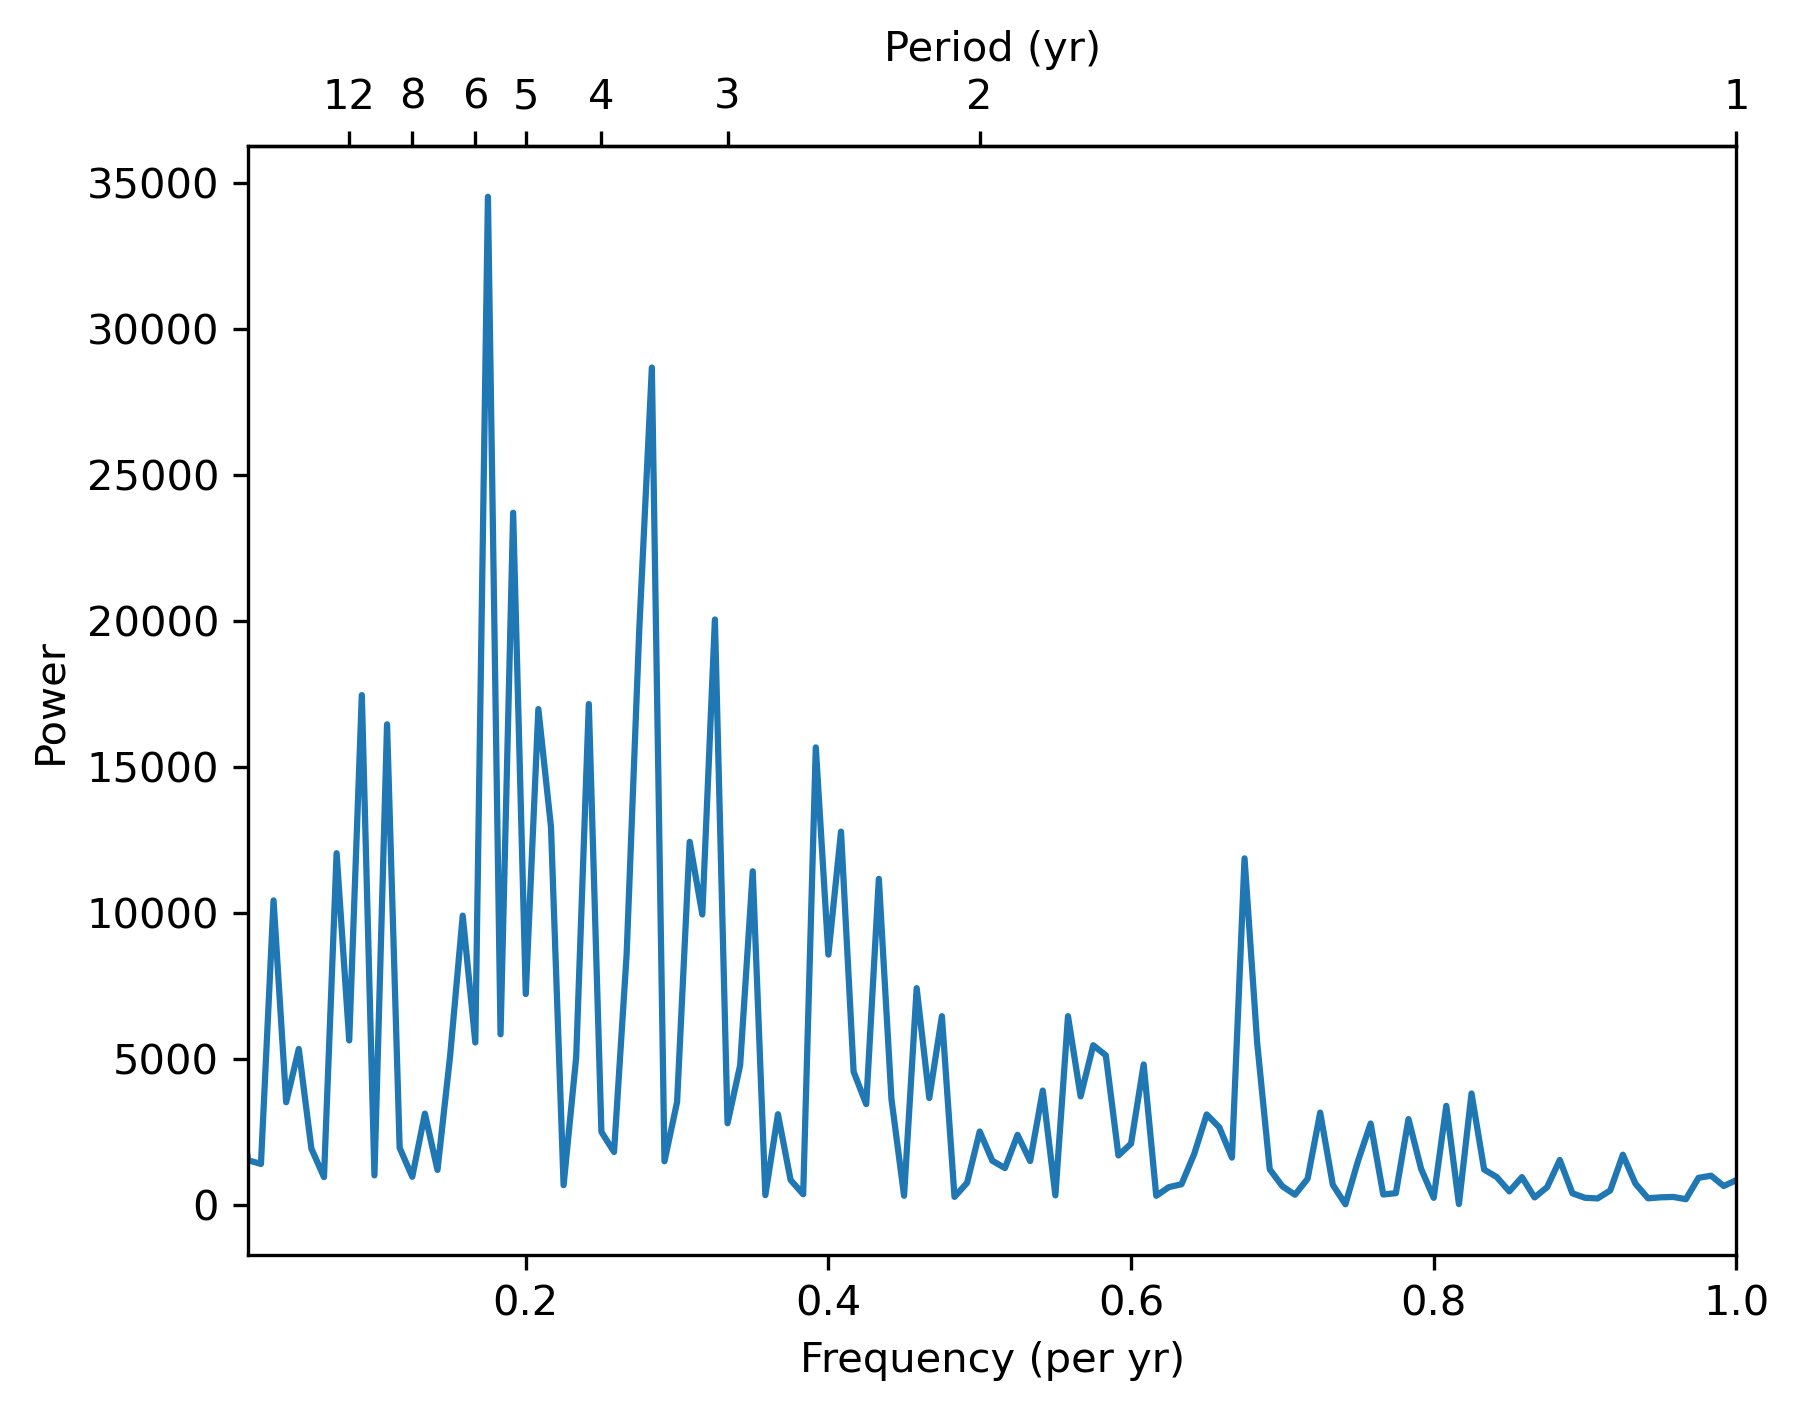
\includegraphics[scale=0.75]{graphics/NinoFFT.png}
\end{center}
It can be seen that the strongest signals are located over the periods from $2.5$ to $7$ years, which coincides with the typical time scale of ENSO. We can carry out a simple filtering to extract the Niño 3.4 signals corresponding to ENSO by zeroing out the FFT array at all other frequencies and then apply an inverse FFT: 
\begin{lstlisting}
from scipy.fft import ifft

Nino34_fft_ENSO = np.copy(Nino34_fft)
Nino34_fft_ENSO[~((2.5 <= np.abs(Nino34_period)) & (np.abs(Nino34_period) <= 7))] = 0
Nino34_ENSO = np.real(ifft(Nino34_fft_ENSO))
\end{lstlisting}
Let's make a plot to compare the filtered time-series with the original one.
\begin{lstlisting}
plt.plot(Nino34_120yrs["Date"], Nino34_120yrs["Nino34"].values, label="raw")
plt.plot(Nino34_120yrs["Date"], Nino34_ENSO, label="FFT-filtered")
plt.xticks(np.arange(0,len(Nino34_120yrs["Date"]), 60), rotation=20)
plt.xlim(["1981-01-01", "2020-12-31"])
plt.xlabel("Date")
plt.ylabel("Nino 3.4 Index")
plt.legend()
plt.title("ENSO-filtered Nino 3.4 Time-series")
plt.savefig("NinoENSOFilter")
\end{lstlisting}
However, note that this "zeroing-out" filtering method is not a very good idea to be implemented in practice and we do it here only due to heuristic purpose. For more information, search about the \textit{"Gibbs Phenomenon"} and also read the comprehensive discussion in   \href{https://stackoverflow.com/questions/31256252/why-does-numpy-linalg-solve-offer-more-precise-matrix-inversions-than-numpy-li}{this DSP StackExchange post} (6220).
\begin{center}
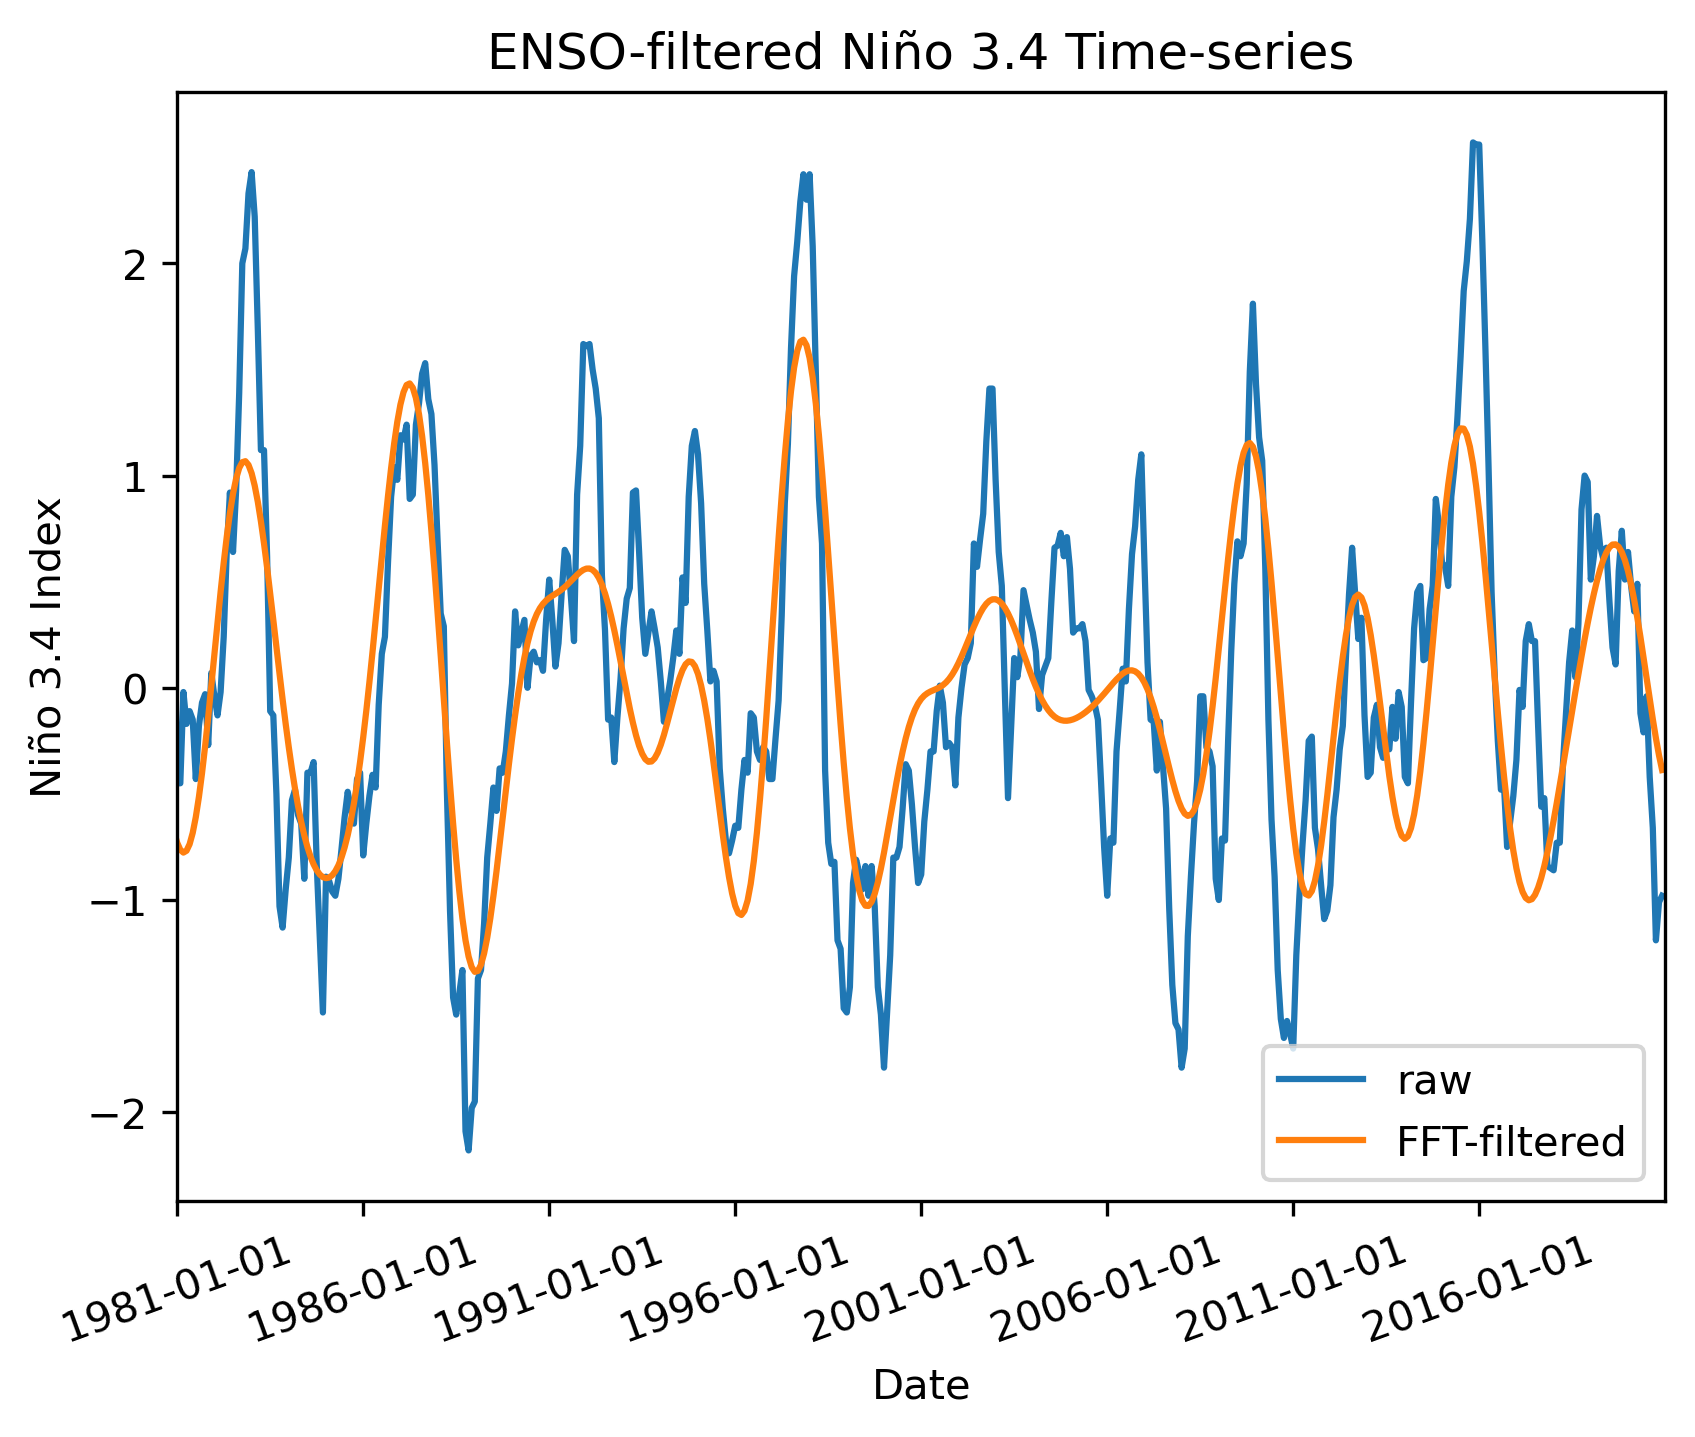
\includegraphics[scale=0.8]{graphics/NinoENSOFilter.png}
\end{center}


\section{Exercise}
\begin{Exercise}
Compute the Discrete Fourier Transform for the following data.
\begin{center}
\begin{tabular}{|c|c|c|c|c|c|c|}
\hline
unit time & 0 & 1 & 2 & 3 & 4 \\
\hline
f(t) & 4.5 & 6.2 & 7.8 & 1.1 & 3.4  \\
\hline
unit time & 5 & 6 & 7 & 8 & 9 \\
\hline
f(t) & 2.5 & 3.6 & 5.9 & 2.9 & 6.0\\
\hline
\end{tabular}
\end{center}
Find the amplitude/power and phase of the sinusoidal wave signal corresponding to the third frequency bin, i.e.\ with an angular frequency of $\omega = 2\pi(\frac{3}{10})$. 
\end{Exercise}

\begin{Exercise}
Download an \href{https://cds.climate.copernicus.eu/datasets/reanalysis-era5-single-levels?tab=download}{ERA5 Temperature dataset} over any time period of $15$ years. Select any location as you like, and extract the temperature time-series there. Apply DFT on the time series, and identify any dominant frequency or period with a large power magnitude. Explain the peaks with Earth Science knowledge.
\end{Exercise}

\begin{Exercise}
Perform DFT on the time-series for the two MJO EOF modes derived in Exercise (\ref{ex:MJO}) and deduce the characterisitc time scale of MJO by plotting the power spectrum against periods.
\end{Exercise}

\begin{Exercise}
Find the circular convolution of two time-series $f(t) = (1,4,2,4, \\ 3,0,-1,2)$ and $g(t) = (2,3,-2,1,-1,0,4,3)$ by definition, as well as via the Convolution Theorem to check the consistency.
\end{Exercise}

\begin{Exercise}
Write your own FFT function in Python and compare with the one in the \verb|scipy.fft| library by testing them on any time-series.
\end{Exercise}
\chapter{Markov Chains}
\label{chapter:Markov}

In Earth Science, we often look at the evolution of variables in time, like temperature, rainfall, etc. Sometimes, the variables can be modeled as \textit{random variables}. A simple daily example will be tossing a coin (no matter if it is fair or not), where the outcomes (head/tail) are probabilistic. Some Earth System examples are the chances of extreme weather and slow geological processes. Such processes involving random variables are known as \textit{Stochastic Processes}, and we will visit the related Statistical concepts. Particularly, we will investigate the so-called \textit{Markov Chains}, which assumes that the present state of a stochastic process only depends on the past. Modeling a stochastic process with a Markov Chain can give more satisfactory results when it is known that the process inherently correlates strongly with previous states, or is said to have \textit{memory}.

\section{Statistical Prerequisites for Markov Chains}

\subsection{Lagged Auto-correlation}

First, let's talk about how to determine if a \index{Time Series}\keywordhl{time series} possesses some sort of \index{Memory}\textit{memory} as mentioned in the introduction. Memory causes the past of a time series to influence the present, and hence will leave a mark when we try to correlate the past and present segments of the time series. This leads to the idea of \index{Lagged (Lag-$k$) Auto-correlation}\keywordhl{lagged auto-correlation}, which is the correlation between a time series and itself, but one of them is lagged and shifted by a certain amount of days, let's say $k$ (the direction of the shifting does not matter as it is an auto-correlation, and we only care about the overlapping part). Then, it is more specifically known as the \textit{Lag-$k$ Auto-correlation}.

\begin{defn}[Lagged Auto-correlation]
\label{defn:autocorr}
The lag-$k$ auto-correlation $r_k$ of a time series $\{x_i\}_{i=1}^{n}$ is defined as 
\begin{align}
r_k &= \frac{\sum_{i=1}^{n-k}(x_i - \overline{x_{-}})(x_{i+k} - \overline{x_{+}})}{\sqrt{(\sum_{i=1}^{n-k}(x_i - \overline{x_{-}})^2) (\sum_{j=k+1}^{n}(x_j - \overline{x_{+}})^2)}}
\end{align}
the correlation (Definition \ref{defn:correlation}) between $\{x_{-}\} = \{x_i\}_{i=1}^{n-k}$ and $\{x_{+}\} = \{x_i\}_{i=k+1}^{n}$ where they are the two sub-sequences extracted from the earliest and latest $n-k$ data of the original time series, and the overline denotes an average. Alternatively, the formula can be written as
\begin{subequations}
\label{eqn:autocorrvar}
\begin{align}
r_k &= \frac{\text{Cov}(\{x_{-}\},\{x_{+}\})}{\sqrt{\text{Var}(\{x_{-}\}) \text{Var}(\{x_{+}\})}} \\
&= \frac{\text{Cov}(\{x_{-}\},\{x_{+}\})}{\sqrt{\text{Cov}(\{x_{-}\}, \{x_{-}\}) \text{Cov}(\{x_{+}\}, \{x_{+}\})}}
\end{align}   
\end{subequations}
where the definitions of variance and covariance are based on Definitions \ref{defn:variance} and \ref{defn:covariance}.
\end{defn}
If the lag-$k$ auto-correlation of a time series is close to $1$ or $-1$, it means that the state at a certain time will likely lead to a similar/opposite state $k$ time steps later. This may be used to infer causality but the implication is not always definite. There may be situations when the generated time series is regarded to be infinitely long, and in such cases, we simply apply the shifting and compute the lagged summation over the entire time axis.

\begin{exmp}
For the traffic flow data over some seven days of a highway below, find its lag-$1$ auto-correlation.
\begin{center}
\begin{tabular}{|c|c|c|c|c|c|c|c|}
\hline
Day & $1$ & $2$ & $3$ & $4$ & $5$ & $6$ & $7$ \\
\hline
Vehicles per Hour & $680$ & $820$ & $760$ & $790$ & $840$ & $1030$ & $1080$ \\
\hline
\end{tabular}
\end{center}
\end{exmp}
We first locate the first and last $7-1 = 6$ data and construct the two smaller time series, which are $\{x_-\} = \{680, 820, 760, 790, 840, 1030\}$ and $\{x_+\} = \{820, 760, 790, 840, 1030, 1080\}$. The means of the two time series are easily found to be $\overline{x_{-}} = 820$ and $\overline{x_{+}} = 2660/3$ (the readers can verify these numbers), and the sample variances of the two time series are thus
\begin{align*}
\text{Var}(\{x_-\}) &= \frac{1}{6-1}[(680 - 820)^2 + (820 - 820)^2 + (760 - 820)^2 \\
& \quad + (790 - 820)^2 + (840 - 820)^2 + (1030 - 820)^2] \\
&=13720 \text{ (Vehicles per Hour)}^2 \\
\text{Var}(\{x_+\}) &= \frac{1}{6-1}\left[\left(820 - \frac{2660}{3}\right)^2 + \left(760 - \frac{2660}{3}\right)^2 + \left(790 - \frac{2660}{3}\right)^2\right. \\
&\quad \left. + \left(840 - \frac{2660}{3}\right)^2 + \left(1030 - \frac{2660}{3}\right)^2 + \left(1080 - \frac{2660}{3}\right)^2\right] \\
&= 17987 \text{ (Vehicles per Hour)}^2
\end{align*}
and their sample covariance is
\begin{align*}
&\quad \text{Cov}(\{x_{-}\},\{x_{+}\}) \\
&= \frac{1}{6-1}\left[(680 - 820)\left(820 - \frac{2660}{3}\right) + (820 - 820)\left(760 - \frac{2660}{3}\right)\right. \\
&\quad + (760 - 820)\left(790 - \frac{2660}{3}\right)  + (790 - 820)\left(840 - \frac{2660}{3}\right) \\
&\quad \left. + (840 - 820)\left(1030 - \frac{2660}{3}\right) + (1030 - 820)\left(1080 - \frac{2660}{3}\right)\right] \\
&= 12000 \text{ (Vehicles per Hour)}^2
\end{align*}
Hence by Formula (\ref{eqn:autocorrvar}) in Definition \ref{defn:autocorr} above, the lag-$1$ auto-correlation is
\begin{align*}
r_1 &= \frac{12000}{\sqrt{(13720)(17987)}} = 0.7639
\end{align*}
It means that heavy (quiet) traffic will likely be followed by more or less heavy (quiet) traffic the next day, which is quite reasonable.\par
$\blacktriangleright$ Short Exercise: Compute the lag-$2$ auto-correlation for the same dataset.\footnotemark

\subsection{Conditional Probabilities, Stochastic Matrices}
To understand the idea of Markov Chains, we also need to know what \textit{conditional probabilities} are. The \index{Conditional Probability}\keywordhl{conditional probability} $P(A|B)$ is the probability of event $A$ occurring, given event $B$ has occurred. For an evolving system that has a finite number of states $A_i$, $i = 1,2,\ldots,n$, and can only possess one state at a time, e.g.\ a binary on-and-off, the conditional probability \smash{$P(A_i^{[k+1]}|A_j^{[k]})$} represents the probability of state $A_i$ occurring at time step $k+1$ if the state is $A_j$ at time step $k$. A simple Atmospheric Sciences example is the daily weather report, which in a simplistic sense, can take the state of either sunny, rainy, or windy. Usually, if it is rainy today, then there is a relatively high chance it is rainy tomorrow, i.e.\ \smash{$P(\text{rainy}^{[k+1]}|\text{rainy}^{[k]})$} is high. \par
For $N$ finite, distinct states/events in a well-defined, \textit{closed} system so that it takes one and only one of the events as its state, we have the following observation.
\begin{proper}
\label{proper:condprobsumto1}
The sum of conditional probabilities for a changing system with $N$ \textit{mutually exclusive} (only one state at a time) and \textit{exhaustive} (the states cover all possibilities) events $A_1, A_2, \cdots, A_N$ is
\begin{align}
\sum_{i=1}^N P(A_i^{[k+1]}|A_j^{[k]}) &= P(A_1^{[k+1]}|A_j^{[k]}) + P(A_2^{[k+1]}|A_j^{[k]}) + \cdots + P(A_N^{[k+1]}|A_j^{[k]}) \nonumber \\
P(\Omega^{[k+1]}|A_j^{[k]}) &= 1
\end{align}
where $\Omega = \bigcup_{i} A_i$ covers all the states and $k$ denotes a particular time step. The time increment is $1$ here but can be replaced by any other positive integer. It means that any given event $A_j$ must consequently lead to one of the possible states (including $A_j$ itself) at the next (few) time step(s).
\end{proper}
\footnotetext{The new $\{x_-\}$ and $\{x_+\}$ will be $\{680, 820, 760, 790, 840\}$ and $\{760, 790, 840, 1030, 1080\}$. We provide the relevant numbers for the readers to check. Their sample (co)variances are $\text{Var}(\{x_-\}) = 3920$, $\text{Var}(\{x_+\}) = 21150$ and $\text{Cov}(\{x_{-}\},\{x_{+}\}) = 5725$. So the lag-$2$ auto-correlation will be $r_2 = \smash{\frac{5725}{\sqrt{(3920)(21150)}}} = 0.6287$.}
This is essentially a rephrasing of the \index{Law of Total Probability}\textit{Law of Total Probability} from elementary Statistics. As a result, we can express all the conditional probabilities \smash{$P(A_i^{[k+1]}|A_j^{[k]})$} for a particular previous state $A_j$ in a system using a column vector with components that sum up to $1$. Using the daily weather as an example, assume there are only three states (sunny/windy/rainy), if a sunny day has a chance of $0.8$ to be followed by another sunny day, and $0.15$/$0.05$ for another windy/rainy day. Then we can write
\begin{center}
\begin{tabular}{|c|c|}
\hline
$k+1 \; \backslash \; k$ & Sunny \\
\hline
Sunny & $0.8$ \\
\hline
Windy & $0.15$ \\
\hline 
Rainy & $0.05$ \\
\hline
\end{tabular}
\end{center}
as a column vector
\begin{align*}
\begin{bmatrix}
0.8 \\
0.15 \\
0.05
\end{bmatrix}
\end{align*}
We can do the same for the other two states. If a windy day has a probability of $0.2$/$0.5$/$0.3$ leading to a sunny/windy/rainy day, and a rainy day has a probability of $0.1$/$0.2$/$0.7$ leading to a sunny/windy/rainy day, then
\begin{center}
\begin{tabular}{|c|c|c|c|}
\hline
$k+1 \; \backslash \; k$ & Sunny & Windy & Rainy \\
\hline
Sunny & $0.8$ & $0.2$ & $0.1$\\
\hline
Windy & $0.15$ & $0.5$ & $0.2$ \\
\hline 
Rainy & $0.05$ & $0.3$ & $0.7$ \\
\hline
\end{tabular}
\end{center}
This can be summarized by the so-called \index{Stochastic Matrix}\keywordhl{stochastic (transition) matrix} as
\begin{align*}
P = 
\begin{bmatrix}
0.8 & 0.2 & 0.1\\
0.15 & 0.5 & 0.2 \\
0.05 & 0.3 & 0.7
\end{bmatrix}
\end{align*}
\begin{defn}[Stochastic Matrix]
\label{defn:stocmat}
The stochastic matrix for a closed system with mutually exclusive and exhaustive events $A_1, A_2, \ldots, A_N$, is
\begin{align}
P =
\begin{bmatrix}
P(A_1^{[k+1]}|A_1^{[k]}) & P(A_1^{[k+1]}|A_2^{[k]}) & \cdots & P(A_1^{[k+1]}|A_N^{[k]})\\
P(A_2^{[k+1]}|A_1^{[k]}) & P(A_2^{[k+1]}|A_2^{[k]}) & & P(A_2^{[k+1]}|A_N^{[k]}) \\
\vdots & & \ddots & \vdots \\
P(A_N^{[k+1]}|A_1^{[k]}) & P(A_N^{[k+1]}|A_2^{[k]}) & \cdots & P(A_N^{[k+1]}|A_N^{[k]})
\end{bmatrix}
\label{eqn:stocP}
\end{align}
where $P_{ij} = P(A_i^{[k+1]}|A_j^{[k]})$ is the conditional probability of the system moving to state $i$ at the next time step from the present state $j$.
\end{defn}
Again, notice that the entries along any column add up to $1$. The $j$-th column holds the conditional probabilities of state $j$ leading to different states at the next time step.

\section{Construction of and Prediction by Markov Chains}

\subsection{State Vector, Steady State}

Processes that can be represented by such stochastic matrices proposed above are known as \index{Markov Chain}\keywordhl{Markov Chains}. It is assumed that the conditional probabilities outlined in the stochastic matrices $P$ do not change in time (\index{Stationary}\textit{stationary}). Given a probability vector (or a \index{State Vector}\keywordhl{state vector}) $\vec{x}^{[k]}$ consisting of the probabilities of having different states at a certain time step $k$, we can calculate the probability vector $\vec{x}^{[k+1]}$ at the next time step $k+1$ as $P\vec{x}^{[k]}$.

\begin{proper}
Given a Markov Chain, with a stochastic matrix $P$ described by (\ref{eqn:stocP}), then the state vector $\vec{x}^{[k+1]}$ at time step $k+1$ is decided by
\begin{align}
\vec{x}^{[k+1]} &= P\vec{x}^{[k]}   
\end{align}
\end{proper}
\begin{proof}
If we look at the $i$-th entry on both sides, we have
\begin{align*}
\vec{x_i}^{[k+1]} &= P_{i1} \vec{x_1}^{[k]} + P_{i2} \vec{x_2}^{[k]} + P_{i3} \vec{x_3}^{[k]} \cdots 
\end{align*}
When explicitly written in terms of (conditional) probabilities, it is
\begin{align*}
P(A_i^{[k+1]}) &= P(A_i^{[k+1]}|A_1^{[k]}) P(A_1^{[k]}) + P(A_i^{[k+1]}|A_2^{[k]}) P(A_2^{[k]}) + \cdots \\
&= \sum_{j=1}^N P(A_i^{[k+1]}|A_j^{[k]}) P(A_j^{[k]})
\end{align*}
which is exactly the manifestation of the \textit{Law of Total Probability} again, given the events are mutually exclusive and exhaustive.
\end{proof} 
Similarly, at the $k+2$-th time step, the probability vector is $\vec{x}^{[k+2]} = P^2\vec{x}^{[k]}$. In general, we have $\vec{x}^{[1]} = P\vec{x}^{[0]}, \vec{x}^{[2]} = P\vec{x}^{[1]} = P(P\vec{x}^{[0]}) = P^2\vec{x}^{[0]}$ and 
\begin{align}
\vec{x}^{[n]} &= P^n\vec{x}^{[0]} & & (\vec{x}^{[k+n]} = P^n\vec{x}^{[k]})  \label{eqn:markovpredict}
\end{align}

\begin{exmp}
\label{exmp:weathermarkov}
Using the previous example of daily weather, the stochastic matrix is
\begin{align*}
P = 
\begin{bmatrix}
0.8 & 0.2 & 0.1\\
0.15 & 0.5 & 0.2 \\
0.05 & 0.3 & 0.7
\end{bmatrix}   
\end{align*}
Find the probabilities of each type of weather occurring on Day 2 and Day 3, if we know that the chances of being sunny/windy/rainy on Day 1 are $0.3$/$0.4$/$0.3$. 
\end{exmp}
\begin{solution}
By Formula (\ref{eqn:markovpredict}) we have just derived, the required state vector is
\begin{align*}
\vec{x}^{[2]} &= P\vec{x}^{[1]} \\
&=
\begin{bmatrix}
0.8 & 0.2 & 0.1\\
0.15 & 0.5 & 0.2 \\
0.05 & 0.3 & 0.7
\end{bmatrix}   
\begin{bmatrix}
0.3 \\
0.4 \\
0.3
\end{bmatrix} \\
&= 0.3
\begin{bmatrix}
0.8 \\
0.15 \\
0.05
\end{bmatrix}
+ 0.4
\begin{bmatrix}
0.2 \\
0.5 \\
0.3
\end{bmatrix}
+ 0.3
\begin{bmatrix}
0.1 \\
0.2 \\
0.7
\end{bmatrix} \\
&=
\begin{bmatrix}
0.35 \\
0.305 \\
0.345
\end{bmatrix}
\end{align*}
So on Day 2, the chances of sunny/windy/rainy are $0.35$/$0.305$/$0.345$. It is emphasized that in the end, the required state vector on the next day is just the linear combination of the column vectors that contain the conditional probabilities, with the weightings specified by the current state vector. Again, it is the Law of Total Probability working. Similarly, for Day 3, the state vector will be
\begin{align*}
\vec{x}^{[3]} &= P\vec{x}^{[2]} = P^2\vec{x}^{[1]} \\
&=
\begin{bmatrix}
0.8 & 0.2 & 0.1\\
0.15 & 0.5 & 0.2 \\
0.05 & 0.3 & 0.7
\end{bmatrix}   
\begin{bmatrix}
0.35 \\
0.305 \\
0.345
\end{bmatrix} \\
&= 0.35
\begin{bmatrix}
0.8 \\
0.15 \\
0.05
\end{bmatrix}
+ 0.305
\begin{bmatrix}
0.2 \\
0.5 \\
0.3
\end{bmatrix}
+ 0.345
\begin{bmatrix}
0.1 \\
0.2 \\
0.7
\end{bmatrix} \\
&=
\begin{bmatrix}
0.3755\\ 
0.274\\
0.3505
\end{bmatrix}
\end{align*}
\end{solution}
$\blacktriangleright$ Short Exercise: Find the state vector on the next day if today is windy.\footnotemark

For a Markov Chain which has been ongoing for a long period of time, and the initial state becomes effectively forgotten (\index{Memoryless}\textit{memoryless}), it is desirable to obtain the \index{Steady-state Vector}\keywordhl{steady-state vector} which represents the "average" probability of every state given no prior knowledge of the initial state. The steady-state vector $\vec{q}$ remains the same for any time step and the probabilities are stationary. Hence, we have 
\begin{align}
\label{eqn:qeqPq}
\vec{q} = P\vec{q} = \cdots = P^n\vec{q}    
\end{align}
Rearrangement of the relation $\vec{q} = P\vec{q}$ gives 
\begin{align}
(I-P)\vec{q} = \textbf{0}    
\end{align}
which can be recognized as an eigenvalue-eigenvector problem (see Section \ref{section:eigensection}): The steady-state vector $\vec{q}$ corresponds to the eigenvector of $P$ with an eigenvalue of $\lambda = 1$. This eigenvector $\vec{q}$ is then found by following the usual procedure to solve the linear system $(I-P)\vec{q} = \textbf{0}$. Some may suspect if this steady-state vector always exists. To address this question, we will first show that one of the eigenvalues in any Markov Chain must be $1$.\footnotetext{It is simply $P\vec{x}$ where $\vec{x} = (0,1,0)^T$ and thus
\begin{align*}
\begin{bmatrix}
0.8 & 0.2 & 0.1\\
0.15 & 0.5 & 0.2 \\
0.05 & 0.3 & 0.7
\end{bmatrix}  
\begin{bmatrix}
0 \\
1 \\
0
\end{bmatrix}
=
\begin{bmatrix}
0.2 \\
0.5 \\
0.3
\end{bmatrix}
\end{align*} so the probabilities are simply given by the components in the second column of the stochastic matrix.}
\begin{proper}
\label{proper:markoveigen1}
The stochastic matrix $P$ of a Markov chain always has an eigenvalue of $\lambda = 1$. The steady state of a Markov Chain is then simply the eigenvector of $P$ that corresponds to the eigenvalue of $\lambda = 1$ as in $(P - \lambda I)\vec{q} = \textbf{0}$, and normalized by the sum of entries so that they add up to $1$.
\end{proper}
\begin{proof}
We will show that the transpose $P^T$ has an eigenvalue of $\lambda = 1$. Then by Properties \ref{proper:eigentransinv}, $P$ must also share this same eigenvalue and we are done. Particularly, we can observe that $\vec{z} = (1,1,1,\ldots,1)^T$ is an eigenvector of $P^T$ that corresponds to the desired eigenvalue of $1$, because
\begin{align*}
P^T \vec{z} &= 
\begin{bmatrix}
P_{11} & P_{21} & \cdots & P_{n1} \\
P_{12} & P_{22} & \cdots & P_{n2} \\
\vdots & & \ddots & \vdots \\
P_{1n} & P_{2n} & \cdots & P_{nn}
\end{bmatrix}
\begin{bmatrix}
1 \\
1 \\
\vdots \\
1
\end{bmatrix}
=
\begin{bmatrix}
P_{11} + P_{21} + \cdots + P_{n1} \\
P_{12} + P_{22} + \cdots + P_{n2} \\
\vdots \\
P_{1n} + P_{2n} + \cdots + P_{nn}
\end{bmatrix}
=
\begin{bmatrix}
1 \\
1 \\
\vdots \\
1
\end{bmatrix}
= \vec{z}
\end{align*}
where by Properties \ref{proper:condprobsumto1} the entries in each column of $P$ sum to one: $P_{1j} + P_{2j} + \cdots + P_{nj} = 1$.
\end{proof}

\begin{exmp}
\label{exmp:dailyweathersteady}
Find the steady-state vector in the last example about daily weather where
\begin{align*}
P = 
\begin{bmatrix}
0.8 & 0.2 & 0.1\\
0.15 & 0.5 & 0.2 \\
0.05 & 0.3 & 0.7
\end{bmatrix}   
\end{align*}
\end{exmp}
\begin{solution}
We seek to solve the linear system
\begin{align*}
I - P = 
\begin{bmatrix}
0.2 & -0.2 & -0.1\\
-0.15 & 0.5 & -0.2 \\
-0.05 & -0.3 & 0.3
\end{bmatrix}   
\end{align*}
and a simple calculation by Gaussian Elimination reveals that the desired eigenvector of $\lambda=1$ is $\vec{q} = (\frac{9}{7}, \frac{11}{14}, 1)^T$ (You may check by substituting this into $(I-P)\vec{q} = \textbf{0}$). Since the probabilities have to add up to $1$, we divide each component by their sum and this yields the steady-state vector $\vec{q} = (\frac{18}{43}, \frac{11}{43}, \frac{14}{43})^T \approx (0.419, 0.256, 0.326)^T$, meaning that there is $41.9\% / 25.6\% / 32.6\%$ chance of having a sunny/windy/rainy day on average.
\end{solution}
Nevertheless, there is a subtlety. We have only shown that there is always an eigenvalue of $1$ (or in general it is the modulus $\abs{\lambda} = 1$ equals to one, as we will see soon) for a Markov Chain, but we don't know if there is only one unique corresponding eigenvector. Consider an extreme example where there exist three states, A, B, and C. State A always leads to state B, which in turn always leads to state C, and state C will always move back to state A. The stochastic matrix is then simply
\begin{align*}
P = \begin{bmatrix}
0 & 0 & 1\\
1 & 0 & 0 \\
0 & 1 & 0
\end{bmatrix}
\end{align*}
It can be found that there are three eigenvalues $\lambda = 1, -\frac{1}{2} + \frac{\sqrt{3}}{2}i, -\frac{1}{2} - \frac{\sqrt{3}}{2}i$ where the two complex eigenvalues have a modulus of $1$ as well. This system can be easily seen to be unstable. Any state vector other than $(\frac{1}{3}, \frac{1}{3}, \frac{1}{3})^T$ (the eigenvector for $\lambda = 1$) will keep oscillating where the components are "cycled". Therefore, the system will not converge to the steady state despite the existence of a "steady-state" vector of $(\frac{1}{3}, \frac{1}{3}, \frac{1}{3})^T$. The imaginary part of the two complex eigenvalues represents a rotation of the two complex eigenvectors and the modulus of $\abs{\lambda} = 1$ means that the magnitude of this rotation will not decay.\footnote{For the complex eigenvalues $\lambda_{\text{c}}$ and complex eigenvectors $\vec{x}_{\text{c}}$, $\norm{P\vec{x}_{\text{c}}}^2 = \norm{\lambda\vec{x}_{\text{c}}}^2 = \abs{\lambda}^2 \norm{\vec{x}_{\text{c}}}^2 = \norm{\vec{x}_{\text{c}}}^2$ as $\abs{\lambda} = 1$. However, the entries of a state vector are always real-valued and it will be a linear combination of these conjugate complex eigenvectors where the imaginary part is exactly canceled out underneath.} So there should be some restriction if the system has to converge to a unique steady state. It turns out that a sufficient condition is whether the Markov Chain is \textit{regular}. To proceed, we need to introduce some terminologies.

\begin{defn}[Regular Markov Chain]
\label{defn:regularstoc}
A stochastic matrix $P$, or the corresponding Markov Chain, is said to be \index{Regular Markov Chain}\keywordhl{regular} if some power of the stochastic matrix $P^k$, where $k$ is any positive integer, has all positive entries, i.e.\ $P^k$ is a \index{Positive Stochastic Matrix}\keywordhl{positive stochastic matrix} (or simply positive).
\end{defn}

\begin{proper}
\label{proper:positivestoceig}
For a positive stochastic matrix $A$, the only eigenvalue with a modulus $\abs{\lambda} = 1$ is $\lambda = 1$. Moreover, the geometric multiplicity of this eigenvalue $\lambda = 1$ belonging to the matrix $A$ is strictly $1$, i.e.\ there is only one eigenvector corresponding to $\abs{\lambda} = 1$.
\end{proper}
The proof is provided in Appendix \ref{section:Markovappend}. For a regular stochastic matrix $P$, $A = P^k$ is positive for some $k$ by Definition \ref{defn:regularstoc} and hence the only eigenvalue of $P^k$ that has a modulus of $1$ is $\lambda = 1$ and its geometric multiplicity is $1$ by Properties \ref{proper:positivestoceig} above. It is not hard to show that, therefore, $P$ will also have $\lambda = 1$ as the only eigenvalue that has a modulus of one, $\abs{\lambda} = 1$, and the geometric multiplicity is also $1$.\footnotemark{} Hence by combining the two results, we have
\begin{proper}
\label{proper:regularmarkovsteady}
A regular Markov chain always has a unique steady-state vector with an eigenvalue of $1$.  
\end{proper}
The stochastic matrix in Example \ref{exmp:dailyweathersteady} is obviously regular, hence we have been able to derive the steady state for it. However, note that Properties \ref{proper:regularmarkovsteady} provides a sufficient condition only, and a non-regular Markov chain may still converge to a unique steady state. Take\footnotetext{Assume the contrary that there are two different eigenvectors of $P$, $\vec{q}^{(1)}$ and $\vec{q}^{(2)}$, the eigenvalues of which have a modulus $\abs{\lambda_1} = \abs{\lambda_2} = 1$ of one. Then $\smash{P^k\vec{q}^{(1)}} = \smash{P^{k-1}(P\vec{q}^{(1)})} = \lambda_1 \smash{P^{k-1}\vec{q}^{(1)}} = \lambda_1 \smash{P^{k-2} (P\vec{q}^{(1)})} = \smash{\lambda_1^2 P^{k-2}\vec{q}^{(1)}} = \cdots = \smash{\lambda_1^k} \vec{q}^{(1)}$, and similarly we have $P^k\vec{q}^{(2)} = \smash{\lambda_2^k} \vec{q}^{(2)}$. These show that $\vec{q}^{(1)}$ and $\vec{q}^{(2)}$ will be also two eigenvectors to $A = P^k$ with an eigenvalue of $\lambda_1^k$ and $\lambda_2^k$ where both of their modulus $\smash{\abs{\lambda_j^k}} = \abs{\lambda_j}^k = 1$, $j = 1,2$, equal to one, contradicting Properties \ref{proper:positivestoceig}.}
\begin{align*}
P = 
\begin{bmatrix}
1 & 0.5 \\
0 & 0.5
\end{bmatrix}
\end{align*}
as an example. It is not hard to see that the bottom-left entry in $P^k$ where $k$ is any positive integer, will always be $0$.\footnote{In general, for any two $2 \times 2$ matrices both in the form of
\begin{align*}
\begin{bmatrix}
* & * \\
0 & *    
\end{bmatrix}
\end{align*} their product
\begin{align*}
\begin{bmatrix}
* & * \\
0 & *    
\end{bmatrix}
\begin{bmatrix}
* & * \\
0 & *    
\end{bmatrix}
=
\begin{bmatrix}
* & * \\
(0)(*) + (*)(0) & *    
\end{bmatrix}
=
\begin{bmatrix}
* & * \\
0 & *    
\end{bmatrix}
\end{align*} will take such a form too.} However, it is also easy to see that given any starting probability vector, it will approach the steady-state vector $(1,0)^T$ as it goes on. Another problem is that in Definition \ref{defn:regularstoc} we haven't specified how large the $k$ we have to keep checking and when we can stop. For the small example above and by the accompanying footnote, knowing $P^2$ is not positive is adequate to decide that it is not regular. For completeness, we note that in general, given an $n \times n$ stochastic matrix $P$, the required $k$ to test is up to $n^2 - 2n + 2$ (so for $n = 2$, we will check $k = 1,2$; and $n = 3$, $k = 1,2,3,4,5$).\footnote{This "magic number" is due to a result by Wielandt but the proof is a bit too advanced to be included here.}

\subsection{Expected Value Problem}
For the special case in which one of the states in Markov Chain is \textit{absorbing}, i.e.\ the probability of staying in this node/state is $1$ and the probabilities of moving to other states are all $0$, all pathways will eventually lead to accumulation in this particular \textit{sink} no matter what the initial state is. This is referred to as an \index{Absorbing Markov Chain}\keywordhl{absorbing Markov Chain} and it is possible to predict the expected time needed for any state to arrive at the absorbing state. Note that the previous example of
\begin{align*}
P = 
\begin{bmatrix}
1 & 0.5 \\
0 & 0.5
\end{bmatrix}    
\end{align*}
is exactly an absorbing Markov Chain where the sink is in the first node.
\par

We can attack this problem by finding the total expected time spent in other non-absorbing nodes which is equivalent to the expected time to arrive at the sink. At the zeroth time step, or $t=0$, the time spent in the starting node and other nodes is one and zero unit time respectively. At $t=k$, the average times spent during the $k$-th time step in different nodes are exactly the probabilities of landing on these nodes after $k$ time steps. \par
Hence, the idea is to add up the times staying in the non-absorbing nodes over every time step. Therefore, we consider the variant of the stochastic matrix in which the row and column of the absorbing state are deleted. Assume that there are three states in the absorbing Markov Chain, and its stochastic matrix is
\begin{align*}
P &= 
\begin{bmatrix}
0.2 & 0.8 & 0 \\
0.7 & 0 & 0 \\
0.1 & 0.2 & 1
\end{bmatrix}
\end{align*}
Along the third column, the third component is equal to $1$ and the others are $0$, indicating that the third node is absorbing. After deleting the row and column related to the absorbing state, and only looking at those non-absorbing states, we have
\begin{align*}
P_0 &= 
\begin{bmatrix}
0.2 & 0.8\\
0.7 & 0 \\
\end{bmatrix}   
\end{align*}
Assume we start at the first node, i.e.\ the probability vector representing the initial state is $(1, 0)^T$ in this case, the formula to calculate the total staying time in the non-absorbing nodes over all time steps would be
\begin{align*}
I
\begin{bmatrix}
1 \\
0
\end{bmatrix}
+
P
\begin{bmatrix}
1 \\
0
\end{bmatrix}
+
P^2
\begin{bmatrix}
1 \\
0
\end{bmatrix}
+ \cdots 
=
(I + P_0 + P_0^2 + \cdots)
\begin{bmatrix}
1 \\
0
\end{bmatrix}
=
\begin{bmatrix}
t_1 \\
t_2
\end{bmatrix}
\end{align*}
where the first term on L.H.S. is the time staying in other nodes at the zeroth time step, the second term is that at the first time step, and so on. $t_1$ and $t_2$ will be the total expected time spent at nodes $1$ and $2$ throughout the process. For the case where the starting condition is probabilistic, e.g.\ 50\% chance in the first node
and 50\% chance in the second node, we simply change $(1,0)^T$ to $(0.5,0.5)^T$. We can utilize the formula of \index{Geometric Sum (Matrix)}\textit{geometric sum for a matrix}, and generalize it to accommodate more states.
\begin{proper}
The expected time for an initial state in a Markov Chain to be absorbed into the sink (assumed that there is only one sink) can be inferred from the relation
\begin{subequations}
\begin{align}
\begin{bmatrix}
t_1 \\
t_2 \\
t_3 \\
\vdots 
\end{bmatrix}
&= (I + P_0 + P_0^2 + \cdots)\vec{x}^{[0]} \\
&= (I - P_0)^{-1}
\vec{x}^{[0]}
\end{align}    
\end{subequations}
where $P$ is the associated stochastic matrix and $P_0$ is $P$ with the row and column of the absorbing state removed. $\vec{x}^{[0]}$ is the initial state vector, also with the entry corresponding to the absorbing node removed. The required absorption time to the sink is the sum of $t_i$ over all valid $i$. 
\end{proper}
The only caveat is that the formula of geometric sum for a matrix may not hold in the second equality, just like the original formula for a number will fail if the common ratio has a magnitude larger than or equal to $1$. However, it is guaranteed that, for a stochastic matrix without other sinks or closed loops which make traveling from any state to the sink impossible
\begin{align}
(I - P_0)^{-1} = I + P_0 + P_0^2 + \cdots    
\end{align}
indeed holds.\footnote{An equivalent condition is that the original stochastic matrix $P$ only has one eigenvalue with the value of $\lambda = 1$ that represents the sink and there are no other eigenvalues that also have a modulus of $\abs{\lambda} = 1$.}
\begin{exmp}
For the absorbing Markov Chain that we have been discussing, where
\begin{align*}
& P = 
\begin{bmatrix}
0.2 & 0.8 & 0 \\
0.7 & 0 & 0 \\
0.1 & 0.2 & 1
\end{bmatrix}
&
& P_0 = 
\begin{bmatrix}
0.2 & 0.8\\
0.7 & 0 \\
\end{bmatrix}   
\end{align*}
Find the expected time required to reach the third node if we start from the first node.
\end{exmp}
\begin{solution}
We have
\begin{align*}
I - P_0 &= 
\begin{bmatrix}
0.8 & -0.8\\
-0.7 & 1 
\end{bmatrix} 
\end{align*}
It is not hard to obtain (for example, just do it like in Example \ref{exmp:2x2})
\begin{align*}
(I - P_0)^{-1} &= 
\begin{bmatrix}
4.166 & 3.333 \\
2.917 & 3.333
\end{bmatrix} \\
(I - P_0)^{-1}\vec{x}^{[0]} &= 
\begin{bmatrix}
4.166 & 3.333 \\
2.917 & 3.333
\end{bmatrix}
\begin{bmatrix}
1 \\
0
\end{bmatrix} 
=
\begin{bmatrix}
4.166 \\
2.917
\end{bmatrix}
\end{align*}
Hence the expected time required to reach the third node starting from the first node will be just the sum of the first column in $P_0$, $4.166 + 2.917 = 7.083$.
\end{solution}
$\blacktriangleright$ Short Exercise: Find the expected time required to reach the third node if it has $50\%/50\%$ chances to start at the first/second node instead.\footnotemark

\subsection{Lagged Auto-correlation Predicted by Markov Chains}

The last topic we will touch on Markov Chains is their inherent auto-correlation (see the beginning of this chapter). Consider the simplest case, where a Markov Chain only has two possible states, with a $2 \times 2$ stochastic matrix, in the form of
\begin{align}
P = 
\begin{bmatrix}
P_{11} & P_{12} \\
P_{21} & P_{22}
\end{bmatrix}
=
\begin{bmatrix}
P_{11} & P_{12} \\
1 - P_{11} & 1 - P_{12} \\
\end{bmatrix}
\end{align}
Assume the first/second state represents a value of $1$/$0$ without the loss of generality. The theoretical lag-$1$ auto-correlation between the binary states, predicted by the Markov Chain, can be inferred from (\ref{eqn:autocorrvar}) in Definition \ref{defn:autocorr}, that is
\begin{align*}
r_1 &= \frac{\text{Cov}(\{x_{-}\},\{x_{+}\})}{\sqrt{\text{Var}(\{x_{-}\}) \text{Var}(\{x_{+}\})}} \\
&= \frac{E[X_{-}X_{+}] - E[X_{-}]E[X_{+}]}{\sqrt{(E[X_{-}^2] - (E[X_{-}])^2)(E[X_{+}^2] - (E[X_{+}])^2)}}
\end{align*}
where we have used the short-cut formulae for variance and covariance listed in Section \ref{section:variancesec}. If the Markov Chain has operated for a long enough time, then the means of the two time series, despite lagged by a day, will be equal due to the loss of memory, implying that
\begin{align}
E[X_{-}] = E[X_{+}] &= q_1
\end{align}
where $\vec{q}$ is the steady-state vector, with $q_1$ being the average probability of being in state $1$. Similarly, we have
\begin{align}
E[X_{-}^2] = E[X_{+}^2] &= q_1 
\end{align}
since squaring a time series composed purely of $1$ and $0$ will return itself. The remaining job is to determine $E[X_{-}X_{+}]$, which is\footnotetext{It is simply a matter of computing
\begin{align*}
(I - P_0)^{-1}\vec{x}^{[0]} &= 
\begin{bmatrix}
4.166 & 3.333 \\
2.917 & 3.333
\end{bmatrix}
\begin{bmatrix}
0.5 \\
0.5
\end{bmatrix}=
\begin{bmatrix}
3.75 \\
3.125
\end{bmatrix}
\end{align*}
where $\vec{x}^{[0]}$ is now $(0.5, 0.5)^T$ and the required time is then $3.75 + 3.125 = 6.875$.}
\begin{align}
E[X_{-}X_{+}] &= P(X_{+}=1 \text{ and } X_{-}=1) \nonumber \\
&= P(X_{+}=1|X_{-}=1) P(X_{-}=1) \nonumber \\
&= P_{11} q_1
\end{align}
as per the definition of conditional probability. So the lag-$1$ auto-correlation is
\begin{align}
r_1 &= \frac{(P_{11}q_1-q_1^2)}{\sqrt{(q_1-q_1^2)(q_1-q_1^2)}} \nonumber \\
&= \frac{q_1(P_{11}-q_1)}{(q_1-q_1^2)} \nonumber \\
&= \frac{P_{11}-q_1}{1-q_1} \label{eqn:binaryr1}
\end{align}
But, by the definition of the stationary eigenvector $P\vec{q} = \vec{q}$ in (\ref{eqn:qeqPq}), considering its first component we have
\begin{align}
P_{11}q_1 + P_{12}q_2 &= q_1  \nonumber \\
P_{11}q_1 + P_{12}(1-q_1) &= q_1 \nonumber  \\
(1 - P_{11} + P_{12}) q_1 &= P_{12}
\end{align}
Substituting this into the formula of lag-$1$ auto-correlation (\ref{eqn:binaryr1}) just derived, we arrive at
\begin{align}
r_1 = \frac{P_{11}-q_1}{1-q_1} &= \frac{(1 - P_{11} + P_{12})(P_{11}-q_1)}{(1 - P_{11} + P_{12})(1-q_1)}  \nonumber \\
&= \frac{P_{11}(1 - P_{11} + P_{12}) - (1 - P_{11} + P_{12})q_1}{1 - P_{11} + P_{12} - (1 - P_{11} + P_{12})q_1}  \nonumber \\
&= \frac{P_{11}(1 - P_{11} + P_{12}) - P_{12}}{1 - P_{11} + P_{12} - P_{12}} \nonumber  \\
&= \frac{(1-P_{11})(P_{11}-P_{12})}{1 - P_{11}} \nonumber  \\
&= P_{11} - P_{12}
\end{align}
Therefore, the magnitude of lag-$1$ auto-correlation predicted by a binary Markov Chain is simply the difference between the two conditional probabilities on the same row in the stochastic matrix. By the same essence, the lag-$k$ auto-correlation can be inferred from $r_k = Q_{11} - Q_{12}$, where $Q = P^k$. Fortunately, due to the structure of stochastic matrices, we can derive a straightforward formula for lag-$k$ auto-correlation, which is just the $k$-th power of the lag-$1$ auto-correlation, $r_k = r_1^k$.

\begin{proper}
The lag-$k$ auto-correlation of a binary Markov Chain, associated with a stochastic matrix $P$, is
\begin{align}
r_k = (P^k)_{11} - (P^k)_{12} = (P_{11} - P_{12})^k = r_1^k
\end{align}
where $r_1 = P_{11} - P_{12}$.
\end{proper}
\begin{proof}
The formula holds for $k=1$ as we just see, and now we will prove the equality $(P^k)_{11} - (P^k)_{12} = (P_{11} - P_{12})^k$ for any general $k$. First, it is instructive to find the eigenvalues and eigenvectors of $P$ and diagonalize the matrix. We set out to solve the characteristic equation
\begin{align}
\det(P - \lambda I) =
\begin{vmatrix}
P_{11} - \lambda & P_{12} \\
1 - P_{11} & 1 - P_{12} - \lambda
\end{vmatrix} &= 0 \nonumber \\
(P_{11} - \lambda)(1 - P_{12} - \lambda) - (1 - P_{11})P_{12} &= 0 \nonumber \\
P_{11} - P_{11}P_{12} - \lambda P_{11} - \lambda + \lambda P_{12} + \lambda^2 - P_{12} + P_{11}P_{12} &= 0 \nonumber \\ 
(P_{11} - P_{12}) - \lambda (1 + (P_{11} - P_{12})) + \lambda^2 &= 0 \nonumber\\ 
(1-\lambda)((P_{11} - P_{12})-\lambda)&= 0
\end{align}
So the eigenvalues are $\lambda_1 = 1$ (as expected) and $\lambda_2 = P_{11} - P_{12}$. It is not hard to find the steady-state vector (not yet normalized) $\vec{q}$ that corresponds to $\lambda = 1$, which is
\begin{align}
\vec{q} = 
\begin{bmatrix}
P_{12} \\
1 - P_{11} 
\end{bmatrix}
\end{align}
and we leave it to the readers to check. For $\lambda_2 = P_{11} - P_{12}$, the eigenvector can also be easily found from 
\begin{align*}
& \left[\begin{array}{@{}cc|c@{\,}}
P_{11} - (P_{11} - P_{12}) & P_{12} & 0 \\
1 - P_{11} & 1 - P_{12} - (P_{11} - P_{12}) & 0 \\
\end{array}\right]  \\
=& 
\left[\begin{array}{@{}wc{32pt}wc{30pt}|c@{\,}}
P_{12} & P_{12} & 0 \\
1 - P_{11} & 1 - P_{11} & 0 \\
\end{array}\right]  \\
\to& \left[\begin{array}{@{}wc{32pt}wc{30pt}|c@{\,}}
1 & 1 & 0 \\
1 - P_{11} & 1 - P_{11} & 0 \\
\end{array}\right] & \frac{1}{P_{12}}R_1 \to R_1 \\
\to& \left[\begin{array}{@{}wc{32pt}wc{30pt}|c@{\,}}
1 & 1 & 0 \\
0 & 0 & 0 \\
\end{array}\right] & R_2 - (1 - P_{11})R_1 \to R_2
\end{align*}
hence it has a very simple form of $(-1, 1)^T$. Using the same technique as in Example \ref{exmp:powerdiag}, we diagonalize $P$ according to $S^{-1}PS = D$ where now we use $S$ to denote the matrix formed by the eigenvectors of $P$, and then
\begin{align}
P^k &= (SDS^{-1})^k \nonumber \\
&= (SDS^{-1})(SDS^{-1}) \cdots (SDS^{-1})(SDS^{-1}) \nonumber \\
&= SD (S^{-1}S)D \cdots D (S^{-1}S) DS^{-1} = SD^kS^{-1} \nonumber \\
&= 
\begin{bmatrix}
P_{12} & -1 \\
1 - P_{11} & 1
\end{bmatrix}
\begin{bmatrix}
1 & 0 \\
0 & (P_{11} - P_{12})^k
\end{bmatrix}
\begin{bmatrix}
P_{12} & -1 \\
1 - P_{11} & 1
\end{bmatrix}^{-1} \nonumber \\
&= 
\begin{bmatrix}
P_{12} & -(P_{11} - P_{12})^k \\
1 - P_{11} & (P_{11} - P_{12})^k
\end{bmatrix}
\left(\frac{1}{P_{12} + (1 - P_{11})}
\begin{bmatrix}
1 & 1 \\
-(1 - P_{11}) & P_{12} \\
\end{bmatrix}
\right) \nonumber \\
&= 
\frac{1}{P_{12} + (1 - P_{11})}
\scriptsize
\begin{bmatrix}
P_{12} + (1-P_{11})(P_{11}-P_{12})^k & P_{12} - P_{12}(P_{11}-P_{12})^k \\
(1-P_{11}) - (1-P_{11})(P_{11}-P_{12})^k & (1-P_{11}) + P_{12}(P_{11}-P_{12})^k
\end{bmatrix}
\end{align}
So
\begin{align*}
&\quad (P^k)_{11} - (P^k)_{12} \\
&= \frac{(P_{12} + (1-P_{11})(P_{11}-P_{12})^k) - (P_{12} - P_{12}(P_{11}-P_{12})^k)}{P_{12} + (1 - P_{11})}\\
&= \frac{((1-P_{11}) + P_{12})(P_{11}-P_{12})^k}{P_{12} + (1 - P_{11})} = (P_{11} - P_{12})^k    
\end{align*}
the desired formula is established.
\end{proof}

For instance, given a two-state Markov Chain with the stochastic matrix
\begin{align*}
P = 
\begin{bmatrix}
0.35 & 0.75 \\
0.65 & 0.25
\end{bmatrix}
\end{align*}
Its lag-$1$ auto-correlation will be $0.35 - 0.75 = 0.25 - 0.65 = -0.4$, and the lag-$4$ auto-correlation will be $(-0.4)^4 = 0.0256$. As just shown, the lag-$k$ auto-correlation of any (first-order) binary Markov Chain always decays exponentially.

\section{Python Programming and Earth System Applications}

Let's use the 2024 Hualien Earthquake sequence, the mainshock of which occurred on April 3rd as an illustration. First, download the .csv records from \href{https://scweb.cwa.gov.tw/en-us/earthquake/data}{https://scweb.cwa.gov.tw/en-us/earthquake/data} for April and May. We will first read the data in April and extract the largest earthquake magnitude each day.
\begin{lstlisting}
import numpy as np
import pandas as pd

equake_Apr = pd.read_csv("Seismic activity_April.csv", usecols=np.arange(7), parse_dates=["Orgin date"])
equake_Apr_daily_mag_max = equake_Apr.groupby(equake_Apr["Orgin date"].dt.day)["Magnitude"].max()
\end{lstlisting}
Write a custom function to separate the cases into three levels of magnitude: $6.0$--$6.9$ $\to 0$, $5.0$--$5.9$ $\to 1$, $4.0$--$4.9$ $\to 2$.
\begin{lstlisting}
# Three magnitude classes: 4.0-4.9, 5.0-5.9, 6.0-6.9
def classify_mag(mag):
    if mag >= 6.0:
        return(0)
    elif (5.0 <= mag <= 5.9):
        return(1)
    elif (mag <= 4.9):
        return(2)
\end{lstlisting}
Now comes the main part. Shift the categorized time series by one day and count the incidence of transitions between different states using \verb|np.unique| and the function above, to construct the stochastic matrix.
\begin{lstlisting}
equake_Apr_prev_states = (equake_Apr_daily_mag_max.loc[3:29].apply(classify_mag)).values
equake_Apr_next_states = (equake_Apr_daily_mag_max.loc[4:30].apply(classify_mag)).values

transition_matrix = np.zeros([3,3])
trans_states, Apr_counts = np.unique(np.c_[equake_Apr_next_states, equake_Apr_prev_states], return_counts=True, axis=0)

transition_matrix[trans_states[:,0], trans_states[:,1]] = Apr_counts
transition_matrix = transition_matrix/np.sum(transition_matrix, axis=0)
\end{lstlisting}
We have normalized the columns by their respective sums. Finally, we compute the steady-state eigenvector for this Markov Chain. (Note that the eigenvalue of $1$ will be the one with the largest modulus.)
\begin{lstlisting}
import scipy.linalg as linalg

eigvals, eigvecs = linalg.eig(transition_matrix)
q = eigvecs[:, np.argmax(np.abs(eigvals))] / np.sum(eigvecs[:, np.argmax(np.abs(eigvals))])
print(q)
\end{lstlisting}
This gives \verb|[0.0767 0.4063 0.5170]|, which means that on average, during the active period on any day, the magnitude of the most intense earthquake will have $7.7\%$/$40.6\%$/$51.7\%$ to be $\leq 4.9$, within $5.0$--$5.9$, and $\geq 6.0$ respectively. This is obtained over the training dataset. Now let's read the file for May and see if the actual probabilities match those expected by our Markov Chain formulated from data in April.
\begin{lstlisting}
equake_May = pd.read_csv("Seismic activity_May.csv", usecols=np.arange(7), parse_dates=["Orgin date"])
equake_May_daily_mag_max = equake_May.groupby(equake_May["Orgin date"].dt.day)["Magnitude"].max()
equake_May_states = (equake_May_daily_mag_max.apply(classify_mag)).values
May_counts = np.bincount(equake_May_states)
May_expected_counts_from_Markov = q*31
print(May_counts, May_expected_counts_from_Markov)
\end{lstlisting}
which returns \verb|[2 5 24]| and \verb|[2.4 12.6 16.0]| correspondingly. There are differences clearly in the last two bins and we can confirm it using the \textit{Chi-square Test}:
\begin{lstlisting}
from scipy.stats import chisquare
print(chisquare(f_obs=May_counts, f_exp=May_expected_counts_from_Markov))  
\end{lstlisting}
that yields a $p$-value of \verb|0.0135| which exceeds the $5\%$ significance level. Therefore, we can conclude that the actual distribution of Earthquake events over the testing set deviates from that predicted by the Markov Chain with $95\%$ confidence. This makes both logical and physical sense. Earthquakes are dynamic processes, which means that the transition probabilities will not be stationary, violating the most fundamental assumption of a Markov Chain. Moreover, we implicitly use a first-order Markov Chain in which the current state only depends on the previous day. However, the more earlier earthquakes will also consume the accumulated stress in the tectonic plates, influencing and retarding much later earthquake events, so the Markov process should be a higher-order one. Particularly, the seismic activity should decay and its distribution will gradually shift to the dormant side.

\section{Exercise}

\begin{Exercise}
For the island Gu-Nei-Ng-Dou, if it is a sunny day, then the next day has $75\%$ chance of being sunny, $10\%$ chance of being windy, and $15\%$ of being rainy. Meanwhile, a windy day has a $60\%$/$25\%$/$15\%$ chance of leading to a sunny/windy/rainy day, and a rainy day has a $30\%$/$20\%$/$50\%$ chance of leading to a sunny/windy/rainy day. Find:
\begin{enumerate}[label=(\alph*)]
\item the probability of getting a rainy day three days after a rainy day,
\item the steady-state vector for all three types of weather,
\item the probability of getting at least one sunny day today and tomorrow if it was sunny yesterday.
\end{enumerate}
\end{Exercise}
\begin{Answer}
$P=
\begin{bmatrix}
0.75 & 0.6 & 0.3\\
0.1 & 0.25 & 0.2\\
0.15 & 0.15 & 0.5
\end{bmatrix}$
\begin{enumerate}[label=(\alph*)]
\item 
\begin{align*}
\vec{q} &= P^3
\begin{bmatrix}
0\\
0\\
1
\end{bmatrix} \\
&=
\begin{bmatrix}
0.639375&0.636&0.57675\\ 
0.13975&0.143125&0.1595\\ 
0.220875&0.220875&0.26375
\end{bmatrix}
\begin{bmatrix}
0\\
0\\
1
\end{bmatrix} 
=
\begin{bmatrix}
0.57675\\
0.1595\\
0.26375
\end{bmatrix}  
\end{align*}
So the required probability is $26.375\%$.
\item $I-P=
\begin{bmatrix}
0.25 & -0.6 & -0.3\\
-0.1 & 0.75 & -0.2\\
-0.15 & -0.15 & 0.5    
\end{bmatrix}$,\\
and the eigenvector (normalized to the steady-state vector) for $\lambda = 1$ can be found to be $(0.6244, 0.1448, 0.2308)^T$.
\item
\begin{align*}
&\quad \text{The required probability} \\
&= P(\text{today is sunny}) + P(\text{today is not sunny and tomorrow is sunny})\\
&= 0.75 + (0.1 \times 0.6 + 0.15 \times 0.3) \\
&= 0.855
\end{align*}
\end{enumerate}
\end{Answer}

\begin{Exercise}
Go to \href{https://ggweather.com/enso/oni.htm}{https://ggweather.com/enso/oni.htm} for the historical yearly ENSO status and construct a Markov Chain for the El Niño/La Niña/Neutral conditions.
\end{Exercise}

\begin{Exercise}
\label{ex:15.3}
For the carbon cycle shown below (Figure \ref{fig:ex15.3}), calculate the rate constant $k = \frac{\text{flux}}{\text{stock mass}}$ for each transport process, and verify that on average it takes about 213000 years for carbon in the ocean reservoir to be buried in the sediment by (a) absorbing Markov Chain, (b) considering the biosphere-atmosphere-ocean as a single reservoir and calculating the lifetime $\tau = \frac{1}{k} = \frac{\text{total stock mass}}{\text{flux}}$. Also, if the pathway to the sediment is neglected, find the steady-state vector of the biosphere-atmosphere-ocean system and confirm they are already in a steady state as one would expect.
\begin{figure}
    \centering
    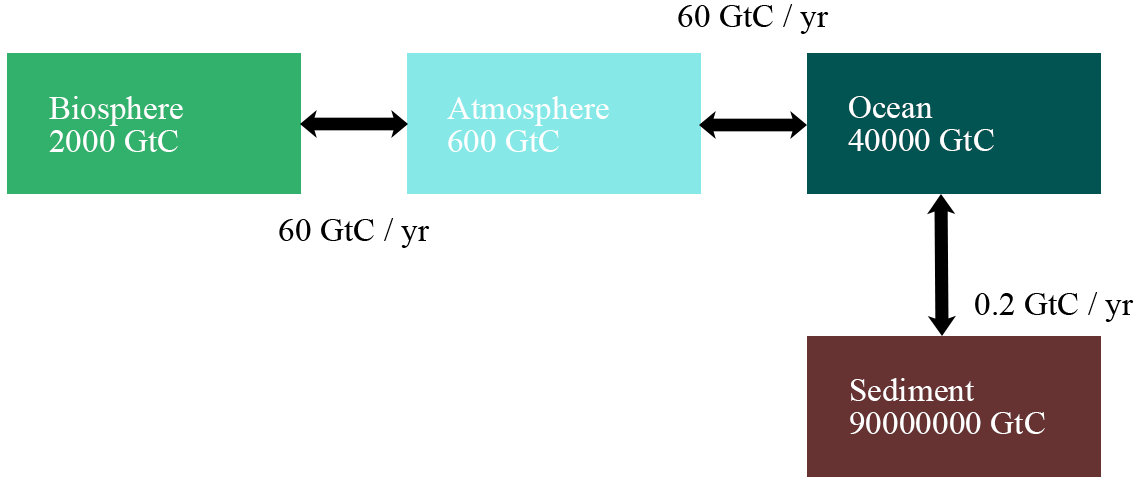
\includegraphics[scale = 1.1]{graphics/carboncycle.png}
    \caption{\textit{Transport between reservoirs in Exercise \ref{ex:15.3}.}}
    \label{fig:ex15.3}
\end{figure}
\end{Exercise}
\begin{Answer}
Node 1/2/3/4: Biosphere/Atmosphere/Ocean/Sediment. $k_{21} = 0.03$, $k_{12} = 0.1$,
$k_{32} = 0.1$, $k_{23} = 0.0015$, $k_{43} = 0.000005$.
\begin{enumerate}[label=(\alph*)]
\item
\begin{align*}
P &= 
\begin{bmatrix}
0.97 & 0.1 & 0 & 0\\
0.03 & 0.8 & 0.0015 & 0\\
0 & 0.1 & 0.998495 & 0\\
0 & 0 & 0.000005 & 1
\end{bmatrix} \\
P_0 &= 
\begin{bmatrix}
0.97 & 0.1 & 0\\
0.03 & 0.8 & 0.0015\\
0 & 0.1 & 0.998495
\end{bmatrix} \\
I-P_0 &=
\begin{bmatrix}
0.03 & -0.1 & 0\\
-0.03 & 0.2 & -0.0015\\
0 & -0.1 & 0.001505
\end{bmatrix} \\
(I-P_0)^{-1} &=
\begin{bmatrix}
10066.66 & 10033.33 & 10000\\
3010 & 3010 & 3000\\
200000 & 200000 & 200000
\end{bmatrix} 
\end{align*}
The sum of the third column is $213000$ yrs.
\item $\tau = \frac{40000+600+2000}{0.2} = 213000$ yrs.
\end{enumerate}
\end{Answer}

\begin{Exercise}
\label{ex:15.4}
Daniel is drunk in a bar. He wants to go to the train station so that he can go home. However, since he is drunk, he loses his sense of direction, and will move randomly along the green edge (shown in the map as Figure \ref{fig:ex15.4} below) once at a time. Assume that at any location, the chances of moving to all other neighboring locations are equal. Nevertheless, once he arrives at the train station, he will stop wandering and take the train. How many moves does it take on average for Daniel to reach the train station?
\begin{figure}
    \centering
    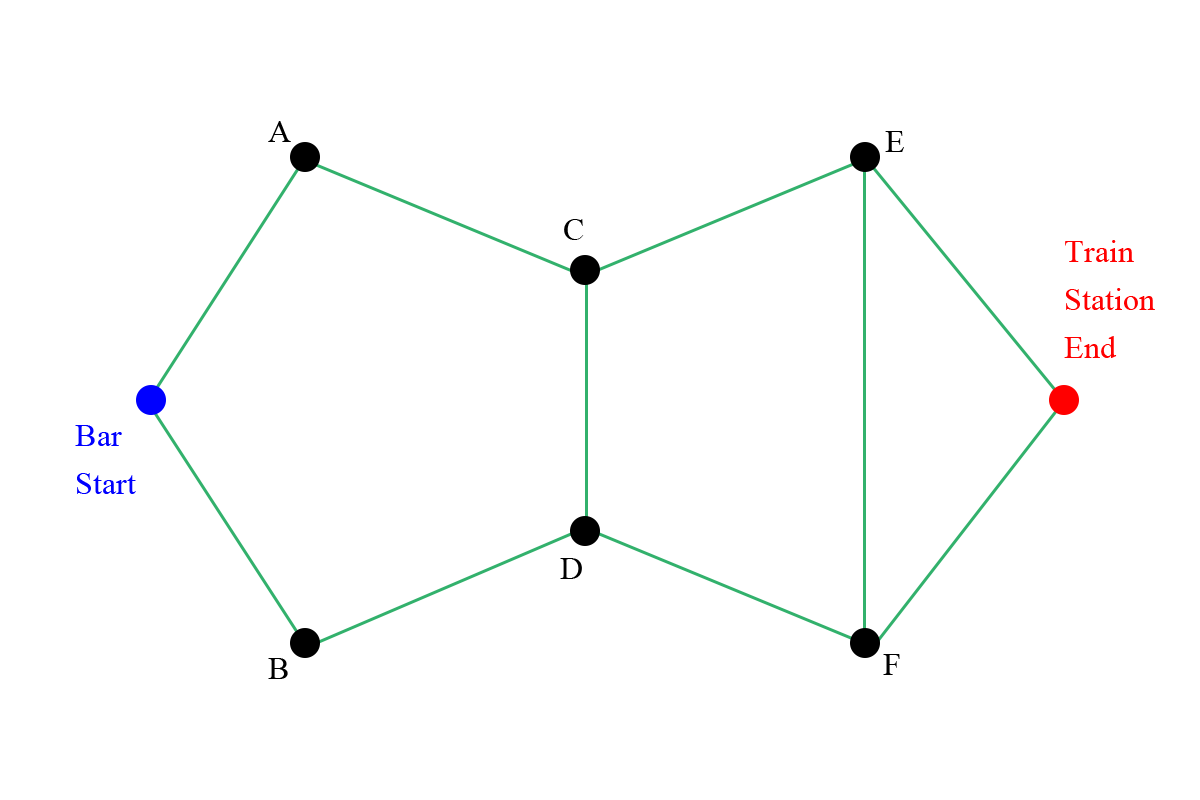
\includegraphics[scale = 0.3]{graphics/wander.png}
    \caption{\textit{The map for Exercise \ref{ex:15.4}.}}
    \label{fig:ex15.4}
\end{figure}
\end{Exercise}
\begin{Answer}
Index 1/2/3/4/5/6/7/8: Start/A/B/C/D/E/F/End. 
\begin{align*}
P_0 &=
\begin{bmatrix}
0 & \frac{1}{2} & \frac{1}{2} & 0 & 0 & 0 & 0\\
\frac{1}{2} & 0 & 0 & \frac{1}{3} & 0 & 0 & 0\\
\frac{1}{2} & 0 & 0 & 0 & \frac{1}{3} & 0 & 0\\
0 & \frac{1}{2} & 0 & 0 & \frac{1}{3} & \frac{1}{3} & 0\\
0 & 0 & \frac{1}{2} & \frac{1}{3} & 0 & 0 & \frac{1}{3}\\
0 & 0 & 0 & \frac{1}{3} & 0 & 0 & \frac{1}{3}\\
0 & 0 & 0 & 0 & \frac{1}{3} & \frac{1}{3} & 0
\end{bmatrix} \\
I - P_0 &= 
\begin{bmatrix}
1&-\frac{1}{2}&-\frac{1}{2}&0&0&0&0\\ 
-\frac{1}{2}&1&0&-\frac{1}{3}&0&0&0\\ 
-\frac{1}{2}&0&1&0&-\frac{1}{3}&0&0\\ 
0&-\frac{1}{2}&0&1&-\frac{1}{3}&-\frac{1}{3}&0\\ 
0&0&-\frac{1}{2}&-\frac{1}{3}&1&0&-\frac{1}{3}\\ 
0&0&0&-\frac{1}{3}&0&1&-\frac{1}{3}\\ 
0&0&0&0&-\frac{1}{3}&-\frac{1}{3}&1
\end{bmatrix} 
\end{align*}
The first column of the inverse $(I - P_0)^{-1}$ can be seen to be $(4,3,3,3,3,\frac{3}{2},\frac{3}{2})^T$ whose sum is $19$, which is the required number of moves.
\end{Answer}

\begin{Exercise}
Attempt \href{https://projecteuler.net/problem=84}{Project Euler Problem 84}, preferably with programming.
\end{Exercise}
\chapter{Matrix Factorization Methods}

In this chapter, we are going to discuss some matrix factorization methods. We have introduced two of them previously: CR Factorization and QR Decomposition, in Chapters \ref{chap:vec_space} and \ref{chap:6x} respectively. We will first discuss two factorization methods for square matrices, \textit{Cholesky} and \textit{LU/LDU}, and subsequently move to the very crucial \textit{Singular Value Decomposition} for non-square matrices. This eventually leads to the notions of \textit{psuedoinverses} and \textit{minimal solutions}. These decomposition methods have been widely applied in many fields of Earth Science to extract important patterns from data. Also, as Machine Learning gains popularity, Earth Science research starts to involve more matrix factorization techniques, which have been a main instrument in Machine Learning. Apart from this, a less visible usage of matrix factorization is embedded in the implementation of linear algebra packages in programming languages (e.g.\ LAPACK, for Fortran). Those matrix factorization methods enable faster and more stable computations of linear algebra problems, such as finding inverses or solving linear systems. Other potential applications include image processing and more.

\section{Square Matrix Factorization}
\subsection{Cholesky Factorization}

\index{Cholesky Decomposition/Factorization}\keywordhl{Cholesky Decomposition} is for the special class of real symmetric and positive-definite matrices. We have talked about how a real symmetric matrix is positive-definite in Section \ref{subsection:definiteness}. For such a matrix $A$, Cholesky Decomposition factorizes it into $U^TU$, where $U$ is an upper-triangular real matrix, and $U^T$ is hence a lower-triangular matrix (remember that upper/lower-triangular implies that non-zero entries are only present along or above/below the main diagonal). An example of Cholesky Factorization would be
\begin{align*}
A = 
\begin{bmatrix}
1 & 0 & 1 \\
0 & 1 & 1 \\
1 & 1 & 6
\end{bmatrix}
&=
\begin{bmatrix}
1 & 0 & 0 \\
0 & 1 & 0 \\
1 & 1 & 2
\end{bmatrix}
\begin{bmatrix}
1 & 0 & 1 \\
0 & 1 & 1 \\
0 & 0 & 2
\end{bmatrix} \\
&= 
\begin{bmatrix}
1 & 0 & 1 \\
0 & 1 & 1 \\
0 & 0 & 2
\end{bmatrix}^T
\begin{bmatrix}
1 & 0 & 1 \\
0 & 1 & 1 \\
0 & 0 & 2
\end{bmatrix} \\
&= U^TU 
\end{align*}
We can compute the Cholesky Decomposition of any positive-definite symmetric matrix step by step, first rewriting the $n \times n$ matrix $A$ into the presumed factorized form of
\begin{align}
A = U^T U = 
\begin{bmatrix}
u_{11} & \vec{r}_1^T \\
\textbf{0} & U_b 
\end{bmatrix}^T
\begin{bmatrix}
u_{11} & \vec{r}_1^T \\
\textbf{0} & U_b 
\end{bmatrix} = 
\begin{bmatrix}
u_{11} & \textbf{0}^T \\
\vec{r}_1 & U_b^T
\end{bmatrix}
\begin{bmatrix}
u_{11} & \vec{r}_1^T \\
\textbf{0} & U_b 
\end{bmatrix}
\end{align}
as a $2 \times 2$ block matrix, where $u_{11}$ will be the first diagonal entry of $U$, $\vec{r}_1$ is a column vector of length $n-1$ and $U_b$ is a submatrix with size $(n-1) \times (n-1)$. The block matrix product (refer to Section \ref{subsection:blockmul}) on R.H.S. gives
\begin{align}
A = 
\begin{bmatrix}
\alpha_{11} & \vec{a}_1^T \\
\vec{a}_1 & \tilde{A}_b 
\end{bmatrix}
=
\begin{bmatrix}
u_{11}^2 & u_{11}\vec{r}_1^T \\
u_{11}\vec{r}_1 & \vec{r}_1\vec{r}_1^T + U_b^T U_b
\end{bmatrix}
= U^TU
\end{align}
where $\alpha_{11}$ is the first diagonal element of $A$, $\vec{a}_1$ and $\tilde{A}_b$ is also a column vector and a submatrix having the same shapes as $\vec{r}_1$ and $U_b$. Comparing the both sides, we have
\begin{subequations}
\begin{align}
\alpha_{11} &= u_{11}^2 \\
\vec{a}_1 &= u_{11}\vec{r}_1 \\
\tilde{A}_b &= \vec{r}_1\vec{r}_1^T + U_b^T U_b
\end{align}    
\end{subequations}
and thus
\begin{subequations}
\begin{align}
u_{11} &= \sqrt{\alpha_{11}} \\
\vec{r}_1 &= \frac{\vec{a}_1}{\sqrt{\alpha_{11}}} \\
U_b^T U_b &= \tilde{A}_b - \vec{r}_1\vec{r}_1^T \label{eqn:UbUbChol}
\end{align}
\end{subequations}
By the relations above, we can determine $u_{11}$, and hence $\vec{r}_1$, retrieving the first row and column of $U$. Subsequently, the remaining block $U_b$ is found by applying the same procedure on the $(n-1) \times (n-1)$ submatrix $U_{b=2}^T U_{b=2}$ which has been produced by the last relation (\ref{eqn:UbUbChol}), and then invoking the method recursively to reduce the resulting block until the final entry is processed.
\begin{defn}[Cholesky Factorization]
The Cholesky Factorization $U^TU$ of a real symmetric, positive-definite matrix $A$, is constructed by the recursive relations
\begin{subequations}
\begin{align}
u_{mm} &= \sqrt{\alpha_{mm}} \label{eqn:cholesky1} \\
\vec{r}_m &= \frac{\vec{a}_m}{\sqrt{\alpha_{mm}}} \label{eqn:cholesky2} \\
U_{b=m+1}^T U_{b=m+1} &= \tilde{A}_{b=m+1} - \vec{r}_m\vec{r}_m^T 
\end{align}    
\end{subequations}
where the subscript $m$ implies we are at the $m$-th step, and
\begin{align}
U_m^T U_m = 
\begin{bmatrix}
\alpha_{mm} & \vec{a}_{m}^T \\
\vec{a}_m & \tilde{A}_{m+1} 
\end{bmatrix}
=
\begin{bmatrix}
u_{mm}^2 & u_{mm}\vec{r}_m^T \\
u_{mm}\vec{r}_m & \vec{r}_m\vec{r}_m^T + U_{m+1}^T U_{m+1}
\end{bmatrix} 
\end{align}
The formulae are iterated over $U_{b=m+1}^T U_{b=m+1}$ acquired at the end of each step.
\end{defn}
We require that at every step, $\alpha_{mm}$ and $u_{mm}$ to be positive so that (\ref{eqn:cholesky1}) and (\ref{eqn:cholesky2}) make sense. It has been shown that matrices in the form of $U^T U$ will always be symmetric, and under this restriction, $U^T U$ will also be positive-definite according to the result in Exercise \ref{ex:sylvesterdefinite}.\footnote{This is because the diagonal elements $u_{mm}$ cannot be zero and thus the upper-triangular $U$ is invertible (why?) so that Exercise \ref{ex:sylvesterdefinite} can apply.} 

\begin{exmp}
\label{exmp:Cholesky}
Perform Cholesky Factorization on the symmetric, positive-definite matrix
\begin{align*}
A &=
\begin{bmatrix}
4 & 2 & 0 \\
2 & 2 & 2 \\
0 & 2 & 5 
\end{bmatrix}
\end{align*}
\end{exmp}
\begin{solution}
The first step results in
\begin{align*}
u_{11} &= \sqrt{\alpha_{11}} = \sqrt{4} = \textcolor{red}{2} \\
\vec{r}_1 &= \frac{1}{\sqrt{\alpha_{11}}}\vec{a}_{1} = \frac{1}{\sqrt{4}}
\begin{bmatrix}
2 \\
0
\end{bmatrix}
= 
\begin{bmatrix}
\textcolor{blue}{1} \\
\textcolor{blue}{0}
\end{bmatrix} \\
U_2^T U_2 = A_2 - \vec{r}_1\vec{r}_1^T &= 
\begin{bmatrix}
2 & 2 \\
2 & 5
\end{bmatrix}
-
\begin{bmatrix}
1 \\
0
\end{bmatrix}
\begin{bmatrix}
1 & 0
\end{bmatrix} \\
&= \begin{bmatrix}
1 & 2 \\
2 & 5 
\end{bmatrix}
\end{align*}
So we know that
\begin{align*}
U &=
\begin{bmatrix}
\textcolor{red}{2} & \textcolor{blue}{1} & \textcolor{blue}{0} \\
0 & ? & ? \\
0 & ? & ? \\
\end{bmatrix}
\end{align*}
Similarly, the next iteration on $U_2^T U$ gives
\begin{align*}
u_{22} &= \sqrt{1} = \textcolor{red}{1} \\  
\vec{r}_2 &= \frac{1}{\sqrt{1}}
\begin{bmatrix}
2
\end{bmatrix}
=
\begin{bmatrix}
\textcolor{blue}{2}
\end{bmatrix} \\
U_3^T U_3 = A_3  - \vec{r}_2\vec{r}_2^T &=
5 - 
\begin{bmatrix}
2
\end{bmatrix}
\begin{bmatrix}
2
\end{bmatrix} \\
&= 
\begin{bmatrix}
1
\end{bmatrix}
\end{align*}
We still need to deal with the $1 \times 1$ matrix that remains. At the third step, we simply take
\begin{align*}
u_{33} = \sqrt{\alpha_{33}} = \sqrt{1} = \textcolor{Green}{1}
\end{align*}
So the final expression of $U$ is given by
\begin{align*}
U = 
\begin{bmatrix}
2 & 1 & 0 \\
0 & \textcolor{red}{1} & \textcolor{blue}{2} \\
0 & 0 & \textcolor{Green}{1}
\end{bmatrix}
\end{align*}
\end{solution}
$\blacktriangleright$ Short Exercise: Check if $A = U^T U$.\footnote{It is simply computing
\begin{align*}
U^TU = 
\begin{bmatrix}
2 & 1 & 0 \\
0 & 1 & 2 \\
0 & 0 & 1
\end{bmatrix}^T
\begin{bmatrix}
2 & 1 & 0 \\
0 & 1 & 2 \\
0 & 0 & 1
\end{bmatrix} =
\begin{bmatrix}
2 & 0 & 0 \\
1 & 1 & 0 \\
0 & 2 & 1
\end{bmatrix}
\begin{bmatrix}
2 & 1 & 0 \\
0 & 1 & 2 \\
0 & 0 & 1
\end{bmatrix} =
\begin{bmatrix}
4 & 2 & 0 \\
2 & 2 & 2 \\
0 & 2 & 5 
\end{bmatrix} = A
\end{align*}
}\par
As a side note, Cholesky Decomposition actually has a very interesting and useful side-effect of determining if a given symmetric matrix is positive-definite. If at any step, $\alpha_{mm}$ is not positive and Formula (\ref{eqn:cholesky1}) fails, then it means that the matrix cannot be positive-definite.\footnote{Heuristically, towards the $m$-th step, we have
\begin{align*}
U_{m}^T U_{m}= 
\begin{bmatrix}
\alpha_{mm} & \cdots \\
\vdots & \ddots
\end{bmatrix}
\end{align*}
and if $\alpha_{mm} \leq 0$ and we set $\vec{w}_{m} = (1,0,\ldots)^T$ where only the first component is $1$ and the others are $0$, we have
\begin{align*}
\vec{w}_{m}^T(U_m^T U_m)\vec{w}_{m} =
\begin{bmatrix}
1 & 0 & \cdots 
\end{bmatrix}
\begin{bmatrix}
\alpha_{mm} & \cdots \\
\vdots & \ddots
\end{bmatrix}
\begin{bmatrix}
1 \\
0 \\
\vdots
\end{bmatrix}
= \alpha_{mm} \leq 0
\end{align*}
which shows that $U_{m}^T U_{m}$ is not positive-definite and it is impossible.}

\subsection{LU/LDU Factorization}

Another method, \index{LU Decomposition/Factorization}\keywordhl{LU Factorization}, is quite similar to Cholesky Factorization. It decomposes any square matrix into one lower and one upper-triangular matrix, $L$ and $U$, but the original matrix does not need to be symmetric or positive-definite. The key to LU factorization is the method of Gaussian Elimination discussed in Sections \ref{section:echelon} and \ref{subsection:invGauss}. Recall that by Gaussian Elimination, we can always reduce a given matrix to an upper-triangular matrix (in row echelon form) during the forward phase, through a sequence of elementary row operations, or equivalently multiplying by the corresponding elementary matrices to the left. Denoting such operations by $E_1', E_2', \cdots, E_m'$ in a spirit similar to the proof of Theorem \ref{thm:Gausselimprincip}, we have $E_m'\cdots E_2'E_1'A = U$, where $U$ is an upper-triangular matrix produced from the forward phase of Gaussian Elimination. Rearrangement gives
\begin{align}
A = (E_1'^{-1}E_2'^{-1}\cdots E_m'^{-1})U    
\end{align}
If none of the $E_i'$ involves row interchange, then they (as well as the inverses $E_i'^{-1}$) would be all lower-triangular matrices (particularly, the multiplicative constant for adding an upper row to a lower row will appear below the main diagonal in that elementary matrix) as required by the forward stage of Gaussian Elimination (meanwhile, if there is row interchange, then $E_i'$ will not be a lower triangular matrix)\footnote{If rows $p$ and $q$ are interchanged, and let's say $p < q$, then above the main diagonal $E_{pq} = 1$.}. As a result, their product $E_1'^{-1}E_2'^{-1}\cdots E_m'^{-1}$ will also be a lower triangular matrix $L$ (see Exercise \ref{ex:triangularprod}):
\begin{align}
L = E_1'^{-1}E_2'^{-1}\cdots E_m'^{-1}    
\end{align}
and the LU Factorization $A = LU$ is consequentially derived.
\begin{thm}[LU Factorization]
The LU Factorization of a square matrix $A$ is possible if it can be reduced to a row echelon form $U$, which will be an upper-triangular matrix, by forward Gaussian Elimination without any row interchange. The steps and elementary matrices used to produce $U$ can be grouped together, and inverted to give a lower triangular matrix $L$ correspondingly. The LU Factorization will then simply be
\begin{align}
A = LU   
\end{align}
\end{thm}

\begin{exmp}
Compute a LU Factorization for
\begin{align*}
A = 
\begin{bmatrix}
2 & 0 & 0 \\
0 & 1 & 1 \\
2 & 0 & 4
\end{bmatrix}
\end{align*}
\end{exmp}
\begin{solution}
By Gaussian Elimination, we have
\begin{align*}
\begin{bmatrix}
2 & 0 & 0 \\
0 & 1 & 1 \\
2 & 0 & 4
\end{bmatrix}
&\rightarrow 
\begin{bmatrix}
1 & 0 & 0 \\
0 & 1 & 1 \\
2 & 0 & 4 
\end{bmatrix}
& E_1' =
\left[\begin{array}{@{\,}wc{10pt}wc{10pt}wc{10pt}@{\,}}
\frac{1}{2} & 0 & 0 \\
0 & 1 & 0 \\
0 & 0 & 1 \\
\end{array}\right]
\\
&\rightarrow 
\begin{bmatrix}
1 & 0 & 0 \\
0 & 1 & 1 \\
0 & 0 & 4 
\end{bmatrix}
&
E_2' =
\left[\begin{array}{@{\,}wc{10pt}wc{10pt}wc{10pt}@{\,}}
1 & 0 & 0 \\
0 & 1 & 0 \\
-2 & 0 & 1 
\end{array}\right]
\\
&\rightarrow 
\begin{bmatrix}
1 & 0 & 0 \\
0 & 1 & 1 \\
0 & 0 & 1
\end{bmatrix}
&
E_3' = 
\left[\begin{array}{@{\,}wc{10pt}wc{10pt}wc{10pt}@{\,}}
1 & 0 & 0 \\
0 & 1 & 0 \\
0 & 0 & \frac{1}{4}
\end{array}\right]
\end{align*}
Therefore, we can take
\begin{align*}
U &= 
\begin{bmatrix}
1 & 0 & 0 \\
0 & 1 & 1 \\
0 & 0 & 1 
\end{bmatrix}
\\
L &= E_1'^{-1}E_2'^{-1}E_3'^{-1} \\
&=
\left[\begin{array}{@{\,}wc{10pt}wc{10pt}wc{10pt}@{\,}}
\frac{1}{2} & 0 & 0 \\
0 & 1 & 0 \\
0 & 0 & 1 
\end{array}\right]^{-1}
\left[\begin{array}{@{\,}wc{10pt}wc{10pt}wc{10pt}@{\,}}
1 & 0 & 0 \\
0 & 1 & 0 \\
-2 & 0 & 1 
\end{array}\right]^{-1}
\left[\begin{array}{@{\,}wc{10pt}wc{10pt}wc{10pt}@{\,}}
1 & 0 & 0 \\
0 & 1 & 0 \\
0 & 0 & \frac{1}{4} 
\end{array}\right]
^{-1} \\
&= \begin{bmatrix}
2 & 0 & 0 \\
0 & 1 & 0 \\
0 & 0 & 1 
\end{bmatrix}
\begin{bmatrix}
1 & 0 & 0 \\
0 & 1 & 0 \\
2 & 0 & 1 
\end{bmatrix}
\begin{bmatrix}
1 & 0 & 0 \\
0 & 1 & 0 \\
0 & 0 & 4 
\end{bmatrix}
\end{align*}
This sequence amounts to the series of elementary row operations in the forward reduction phase. Doing them from the right to the left, it is easy to arrive at
\begin{align*}
L &=
\begin{bmatrix}
2 & 0 & 0 \\
0 & 1 & 0 \\
2 & 0 & 4
\end{bmatrix}
\end{align*}
\end{solution}

Note that LU Factorization is not always unique. However, one can derive \index{LDU Decomposition/Factorization}\keywordhl{LDU Factorization} that is unique whenever an LU decomposition of the matrix exists. Here, $D$ is an extra diagonal matrix while all the diagonal entries $L$ and $U$ are now $1$. Using the above example, we observe that
\begin{align*}
L &=
\begin{bmatrix}
2 & 0 & 0 \\
0 & 1 & 0 \\
2 & 0 & 4
\end{bmatrix} = 
\begin{bmatrix}
1 & 0 & 0 \\
0 & 1 & 0 \\
1 & 0 & 1
\end{bmatrix}
\begin{bmatrix}
2 & 0 & 0 \\
0 & 1 & 0 \\
0 & 0 & 4
\end{bmatrix}
\end{align*}
where we factor out a diagonal matrix from $L$ along each column to its right, to force all the entries along the main diagonal to be $1$. If needed, we can also do the same procedure on $U$ which produces a diagonal matrix to the left instead. So the corresponding LDU Factorization in the previous example is
\begin{align*}
A =
\begin{bmatrix}
1 & 0 & 0 \\
0 & 1 & 0 \\
1 & 0 & 1
\end{bmatrix}
\begin{bmatrix}
2 & 0 & 0 \\
0 & 1 & 0 \\
0 & 0 & 4
\end{bmatrix}
\begin{bmatrix}
1 & 0 & 0 \\
0 & 1 & 1 \\
0 & 0 & 1 
\end{bmatrix}
\end{align*}

There is another variant of LU Factorization which is called \index{PLU Decomposition/Factorization}\keywordhl{PLU Factorization}, applicable to any square matrix $A$. Since the only obstacle to obtaining a LU Decomposition is the presence of row interchanging operations (sometimes necessary, sometimes due to pivoting for numerical stability), the idea is to complete them right from the start so that LU Factorization becomes possible. After obtaining the LU Factorization, we collect all the elementary row matrices involved in the initial row interchanges as a matrix $P$ appended to the left. In practice, we will carry out the forward step of Gaussian Elimination as usual and mark all the row interchanging operations down. The matrix $P$ will simply be the product of all the row interchanging elementary matrices, as swapping rows does not really modify the actual entries and only affects the row indices so that we can move all of them to the left in the end. Whenever we have to move a row interchanging elementary matrix across the other two types of elementary matrices, we can appropriately relocate the addition/multiplication constant $c$ in one of the two rows to another. For example, if we have $R_3 + cR_1 \to R_3$ and $R_2 \leftrightarrow R_3$, then
\begin{align*}
\begin{bmatrix}
1 & 0 & 0 \\
0 & 1 & 0 \\
c & 0 & 1
\end{bmatrix}
\begin{bmatrix}
1 & 0 & 0 \\
0 & 0 & 1 \\
0 & 1 & 0
\end{bmatrix}
=
\begin{bmatrix}
1 & 0 & 0 \\
0 & 0 & 1 \\
0 & 1 & 0
\end{bmatrix}
\begin{bmatrix}
1 & 0 & 0 \\
c & 1 & 0 \\
0 & 0 & 1
\end{bmatrix}
\end{align*}
and if $cR_2 \to R_2$ and $R_2 \leftrightarrow R_3$ this time, we have
\begin{align*}
\begin{bmatrix}
1 & 0 & 0 \\
0 & c & 0 \\
0 & 0 & 1
\end{bmatrix}
\begin{bmatrix}
1 & 0 & 0 \\
0 & 0 & 1 \\
0 & 1 & 0
\end{bmatrix}
=
\begin{bmatrix}
1 & 0 & 0 \\
0 & 0 & 1 \\
0 & 1 & 0
\end{bmatrix}
\begin{bmatrix}
1 & 0 & 0 \\
0 & 1 & 0 \\
0 & 0 & c
\end{bmatrix}
\end{align*}
The same "bubble" logic is similarly applicable to any other pair of indices.
\begin{exmp}
\label{exmp:PLU}
Find a PLU Factorization for
\begin{align*}
A = 
\begin{bmatrix}
1 & 1 & 2 \\
2 & 2 & 3 \\
1 & 3 & 0
\end{bmatrix}
\end{align*}
\end{exmp}
\begin{solution}
We will apply Gaussian Elimination as usual and do the bookmarking for any row interchange.
\begin{align*}
\left[\begin{array}{@{\,}wc{10pt}wc{10pt}wc{10pt}@{\,}}
1 & 1 & 2 \\
2 & 2 & 3 \\
1 & 3 & 0
\end{array}\right]  &\to 
\left[\begin{array}{@{\,}wc{10pt}wc{10pt}wc{10pt}@{\,}}
1 & 1 & 2 \\
0 & 0 & -1 \\
1 & 3 & 0
\end{array}\right] 
&
E_1' =
\left[\begin{array}{@{\,}wc{10pt}wc{10pt}wc{10pt}@{\,}}
1 & 0 & 0 \\
-2 & 1 & 0 \\
0 & 0 & 1
\end{array}\right] \\
&\to 
\left[\begin{array}{@{\,}wc{10pt}wc{10pt}wc{10pt}@{\,}}
1 & 1 & 2 \\
0 & 0 & -1 \\
0 & 2 & -2
\end{array}\right] 
&
E_2' =
\left[\begin{array}{@{\,}wc{10pt}wc{10pt}wc{10pt}@{\,}}
1 & 0 & 0 \\
0 & 1 & 0 \\
-1 & 0 & 1
\end{array}\right] \\
&\to 
\left[\begin{array}{@{\,}wc{10pt}wc{10pt}wc{10pt}@{\,}}
1 & 1 & 2 \\
0 & 2 & -2 \\
0 & 0 & -1 
\end{array}\right] 
&
\textcolor{red}{E_3' =
\left[\begin{array}{@{\,}wc{10pt}wc{10pt}wc{10pt}@{\,}}
1 & 0 & 0 \\
0 & 0 & 1 \\
0 & 1 & 0
\end{array}\right]} \\
&\to 
\left[\begin{array}{@{\,}wc{10pt}wc{10pt}wc{10pt}@{\,}}
1 & 1 & 2 \\
0 & 1 & -1 \\
0 & 0 & -1 
\end{array}\right] 
&
E_4' =
\left[\begin{array}{@{\,}wc{10pt}wc{10pt}wc{10pt}@{\,}}
1 & 0 & 0 \\
0 & \frac{1}{2} & 0 \\
0 & 0 & 1
\end{array}\right] \\
&\to 
\left[\begin{array}{@{\,}wc{10pt}wc{10pt}wc{10pt}@{\,}}
1 & 1 & 2 \\
0 & 1 & -1 \\
0 & 0 & 1 
\end{array}\right] 
&
E_5' =
\left[\begin{array}{@{\,}wc{10pt}wc{10pt}wc{10pt}@{\,}}
1 & 0 & 0 \\
0 & 1 & 0 \\
0 & 0 & -1
\end{array}\right] 
\end{align*} 
So 
\begin{align*}
U = \left[\begin{array}{@{\,}wc{10pt}wc{10pt}wc{10pt}@{\,}}
1 & 1 & 2 \\
0 & 1 & -1 \\
0 & 0 & 1 
\end{array}\right] 
\end{align*}
and we move $E_3'$ all the way to the left and modify $E_1'^{-1}$ and $E_2'^{-1}$ accordingly, to acquire
\begin{align*}
PL &= E_1'^{-1}E_2'^{-1}\textcolor{red}{E_3'^{-1}}E_4'^{-1}E_5'^{-1} \\
&= 
\left[\begin{array}{@{\,}wc{8pt}wc{6pt}wc{7pt}@{\,}}
1 & 0 & 0 \\
-2 & 1 & 0 \\
0 & 0 & 1
\end{array}\right]^{-1}
\left[\begin{array}{@{\,}wc{8pt}wc{6pt}wc{7pt}@{\,}}
1 & 0 & 0 \\
0 & 1 & 0 \\
-1 & 0 & 1
\end{array}\right]^{-1}
\mathcolor{red}{\left[\begin{array}{@{\,}wc{8pt}wc{6pt}wc{7pt}@{\,}}
1 & 0 & 0 \\
0 & 0 & 1 \\
0 & 1 & 0
\end{array}\right]^{-1}}
\left[\begin{array}{@{\,}wc{8pt}wc{6pt}wc{7pt}@{\,}}
1 & 0 & 0 \\
0 & \frac{1}{2} & 0 \\
0 & 0 & 0
\end{array}\right]^{-1}
\left[\begin{array}{@{\,}wc{8pt}wc{6pt}wc{7pt}@{\,}}
1 & 0 & 0 \\
0 & 1 & 0 \\
0 & 0 & -1
\end{array}\right]^{-1} \\
&= 
\left[\begin{array}{@{\,}wc{8pt}wc{6pt}wc{7pt}@{\,}}
1 & 0 & 0 \\
2 & 1 & 0 \\
0 & 0 & 1
\end{array}\right]
\left[\begin{array}{@{\,}wc{8pt}wc{6pt}wc{7pt}@{\,}}
1 & 0 & 0 \\
0 & 1 & 0 \\
1 & 0 & 1
\end{array}\right]
\mathcolor{red}{\left[\begin{array}{@{\,}wc{8pt}wc{6pt}wc{7pt}@{\,}}
1 & 0 & 0 \\
0 & 0 & 1 \\
0 & 1 & 0
\end{array}\right]}
\left[\begin{array}{@{\,}wc{8pt}wc{6pt}wc{7pt}@{\,}}
1 & 0 & 0 \\
0 & 2 & 0 \\
0 & 0 & 0
\end{array}\right]
\left[\begin{array}{@{\,}wc{8pt}wc{6pt}wc{7pt}@{\,}}
1 & 0 & 0 \\
0 & 1 & 0 \\
0 & 0 & -1
\end{array}\right] \\
&= 
\mathcolor{red}{\left[\begin{array}{@{\,}wc{8pt}wc{6pt}wc{7pt}@{\,}}
1 & 0 & 0 \\
0 & 0 & 1 \\
0 & 1 & 0
\end{array}\right]}
\mathcolor{blue}{\left[\begin{array}{@{\,}wc{8pt}wc{6pt}wc{7pt}@{\,}}
1 & 0 & 0 \\
0 & 1 & 0 \\
2 & 0 & 1
\end{array}\right]}
\mathcolor{blue}{\left[\begin{array}{@{\,}wc{8pt}wc{6pt}wc{7pt}@{\,}}
1 & 0 & 0 \\
1 & 1 & 0 \\
0 & 0 & 1
\end{array}\right]}
\left[\begin{array}{@{\,}wc{8pt}wc{6pt}wc{7pt}@{\,}}
1 & 0 & 0 \\
0 & 2 & 0 \\
0 & 0 & 0
\end{array}\right]
\left[\begin{array}{@{\,}wc{8pt}wc{6pt}wc{7pt}@{\,}}
1 & 0 & 0 \\
0 & 1 & 0 \\
0 & 0 & -1
\end{array}\right] \\
&=
\mathcolor{red}{\left[\begin{array}{@{\,}wc{8pt}wc{6pt}wc{7pt}@{\,}}
1 & 0 & 0 \\
0 & 0 & 1 \\
0 & 1 & 0    
\end{array}\right]} 
\left[\begin{array}{@{\,}wc{8pt}wc{6pt}wc{7pt}@{\,}}
1 & 0 & 0 \\
1 & 2 & 0 \\
2 & 0 & -1
\end{array}\right] 
\end{align*}
It is not hard to check that
\begin{align*}
A = \begin{bmatrix}
1 & 1 & 2 \\
2 & 2 & 3 \\
1 & 3 & 0
\end{bmatrix} 
=
\left[\begin{array}{@{\,}wc{8pt}wc{7pt}wc{8pt}@{\,}}
1 & 0 & 0 \\
0 & 0 & 1 \\
0 & 1 & 0    
\end{array}\right] 
\left[\begin{array}{@{\,}wc{8pt}wc{7pt}wc{8pt}@{\,}}
1 & 0 & 0 \\
1 & 2 & 0 \\
2 & 0 & -1
\end{array}\right] 
\left[\begin{array}{@{\,}wc{8pt}wc{7pt}wc{8pt}@{\,}}
1 & 1 & 2 \\
0 & 1 & -1 \\
0 & 0 & 1 
\end{array}\right] 
= PLU
\end{align*}
Notice that PLU Decomposition is not unique as there are many possible ways of doing row exchanges.
\end{solution}
$\blacktriangleright$ Short Exercise: What will the PLU Decomposition in the above example look like if we incorporate the part of "D" as in the LDU variant?\footnote{It will look like
\begin{align*}
A = \begin{bmatrix}
1 & 1 & 2 \\
2 & 2 & 3 \\
1 & 3 & 0
\end{bmatrix} 
=
\begin{bmatrix}
1 & 0 & 0 \\
0 & 0 & 1 \\
0 & 1 & 0    
\end{bmatrix}
\begin{bmatrix}
1 & 0 & 0 \\
1 & 1 & 0 \\
2 & 0 & 1
\end{bmatrix}
\begin{bmatrix}
1 & 0 & 0 \\
0 & 2 & 0 \\
0 & 0 & -1
\end{bmatrix}
\begin{bmatrix}
1 & 1 & 2 \\
0 & 1 & -1 \\
0 & 0 & 1 
\end{bmatrix}
= PLDU
\end{align*}}

\subsection{Solving Linear Systems with LU Decomposition}
As mentioned at the start of this chapter, matrix factorization greatly helps when it comes to electronic calculation. For instance, LU factorization is widely applied to solving linear systems in computers, preferred over direct Gaussian Elimination or using inverses (we will discuss the reasons at the end of the chapter). Basically, it is a two-step procedure. For a linear system $A\vec{x} = \vec{h}$, if we have the LU Decomposition of the matrix $A$, then it can be rewritten as 
\begin{align}
LU\vec{x} = \vec{h}    
\end{align}
Subsequently, we let $U\vec{x} = \vec{y}$, and solve 
\begin{align}
L\vec{y} = \vec{h}
\end{align}
in the first stage, and then come back to solve 
\begin{align}
U\vec{x} = \vec{y}
\end{align}
in the second stage. Due to the triangular nature of $L$ and $U$, we can do a forward and backward substitution respectively to solve the two systems with relative ease.

\begin{exmp}
Solve the linear system $A\vec{x} = \vec{h}$, where
\begin{align*}
A &= 
\begin{bmatrix}
1 & 1 & 0 \\
0 & 2 & 2 \\
1 & 2 & 4 
\end{bmatrix}
& \vec{h} = 
\begin{bmatrix}
3 \\
2 \\
4
\end{bmatrix}
\end{align*}
via LU Factorization.
\end{exmp}
\begin{solution}
We note that one possible LU factorization of $A$ is
\begin{align*}
A &= LU = 
\begin{bmatrix}
1 & 0 & 0 \\
0 & 2 & 0 \\
1 & 1 & 3 
\end{bmatrix}
\begin{bmatrix}
1 & 1 & 0 \\
0 & 1 & 1 \\
0 & 0 & 1 
\end{bmatrix}
\end{align*}
which is left to the readers to verify. We can solve the equivalent problem $LU\vec{x} = \vec{h}$, where we set $U\vec{x} = \vec{y}$ and thus $L\vec{y} = \vec{h}$. The first stage involve solving $L\vec{y} = \vec{h}$:
\begin{align*}
\begin{bmatrix}
1 & 0 & 0 \\
0 & 2 & 0 \\
1 & 1 & 3 
\end{bmatrix}
\begin{bmatrix}
y_1 \\
y_2 \\
y_3
\end{bmatrix}
&=
\begin{bmatrix}
3 \\
2 \\
4
\end{bmatrix}
\end{align*}
By forward substitution from the top to bottom, we have $y_1 = 3$, $2y_2 = 2 \to y_2 = 1$, and $y_1 + y_2 + 3y_3 = (3) + (1) + 3y_3 = 4 \to y_3 = 0$, so $\vec{y} = (3,1,0)^T$. Similarly, we do a backward substitution over $U\vec{x} = \vec{y}$ in the second stage:
\begin{align*}
\begin{bmatrix}
1 & 1 & 0 \\
0 & 1 & 1 \\
0 & 0 & 1 
\end{bmatrix}
\begin{bmatrix}
x_1 \\
x_2 \\
x_3
\end{bmatrix}
=
\begin{bmatrix}
3 \\
1 \\
0
\end{bmatrix}
\end{align*}
which gives $x_3 = 0$, $x_2 + x_3 = x_2 + (0) = 1 \to x_2 = 1$ and $x_1 + x_2 = x_1 + (1) = 3 \to x_1 = 2$, and thus the final answer is $\vec{x} = (2,1,0)^T$.
\end{solution}

To solve a family of linear systems $A\vec{x} = \vec{h}^{(j)}$, where $\vec{h}^{(j)}$ are many different column vectors, can be very time-consuming if we use Gaussian Elimination every time. LU Decomposition extracts and encapsulates the information from Gaussian Elimination, and saves the effort needed to compute Gaussian Elimination for different $\smash{\vec{h}^{(j)}}$ every time since we will only have to do the forward and backward substitution (more details in the answer to this \href{https://math.stackexchange.com/questions/266355/necessity-advantage-of-lu-decomposition-over-gaussian-elimination}{Math Stackexchange post} (266355)). While it is also possible to achieve similar effects by utilizing the inverse $A^{-1}$, calculating the inverse for large systems can be numerically unstable and expensive (which has been discussed in Section \ref{section:ch3python}, and more thoroughly at \href{https://gregorygundersen.com/blog/2020/12/09/matrix-inversion}{https://gregorygundersen.com/blog/2020/12/09/matrix-inversion}).

\section{Singular Value Decomposition (SVD)}

\subsection{Mathematical Ideas of SVD and its Computation}

The previous LU Factorization can also be applied to a non-square matrix. However, there is another very important factorization method called the \index{Singular Value Decomposition (SVD)}\keywordhl{Singular Value Decomposition (SVD)} that is more useful for signal processing, data compression, and feature extraction. SVD proposes that any matrix $A$, no matter square or non-square, can be rewritten into the product of three matrices:
\begin{align}
A = U\Sigma V^* \label{eqn:SVD1}
\end{align}
where $A$ is a given $m \times n$ matrix, $U$ and $V$ are two unitary square matrices of the shape $m \times m$ and $n \times n$ respectively, and $\Sigma$ is an $m \times n$ diagonal\footnote{In this chapter, we generalize and use the word "diagonal" for non-square matrices too, in the sense that non-zero entries only occurs when the row and column indices are equal just like for square matrices.} matrix. The principle of SVD essentially revolves around a generalized orthogonal/unitary change of coordinates for a matrix (or linear transformation). To see this, compare (\ref{eqn:SVD1}) to (\ref{eqn:coordchangelintrans}) in Properties \ref{proper:chcoordsmat} about coordinate transformation for a matrix in general, and set $[T]^{\gamma'}_{\beta'} = \Sigma$, $Q_{\gamma'}^{\gamma} = U$, $[T]^{\gamma}_{\beta} = A$ and $P_{\beta'}^{\beta} = V$. Subsequently, Equation (\ref{eqn:coordchangelintrans}) becomes
\begin{align}
\Sigma = U^{-1}AV    
\end{align}
Since $U$ and $V$ are both unitary (Definition \ref{defn:unitary}, $U^{-1} = U^*$, $UU^* = I = VV^*$), it can be expressed in two ways.
\begin{align*}
\Sigma &= U^*AV \\
\text{as well as \quad} U\Sigma V^* &= UU^*AVV^* \\
&= (UU^*)A(VV^*) = (I)A(I) = A
\end{align*}
So we arrive at (\ref{eqn:SVD1}) again. This means that the central idea of SVD is to find two orthonormal (unitary) bases for the input/output vector spaces $\mathcal{V}$ and $\mathcal{W}$ so that after changing the respective coordinate systems to these two bases, the linear transformation will then have a diagonal representation. As a result, the first step is to show for any linear transformation, we can always find some suitable orthonormal bases for $\mathcal{V}$ and $\mathcal{W}$ so that any basis vector $\vec{v}^{(j)} \in \mathcal{V}$ from the starting vector space is mapped to a constant multiple of one and only one corresponding basis vector $\vec{u}^{(j)} \in \mathcal{W}$ in the other vector space.
\begin{thm}[Singular Value Theorem for Linear Transformations]
\label{thm:SVDtrans}
For two inner product spaces $\mathcal{V}$ and $\mathcal{W}$ of finite dimensions $n$ and $m$ respectively, as well as given a linear transformation $T: \mathcal{V} \to \mathcal{W}$ between them, there exist orthonormal bases $\beta = \{\vec{v}^{(1)}, \vec{v}^{(2)},\ldots,\vec{v}^{(n)}\}$ for $\mathcal{V}$ and $\gamma = \{\vec{u}^{(1)}, \vec{u}^{(2)},\ldots,\vec{u}^{(m)}\}$ for $\mathcal{W}$ so that 
\begin{align}
T(\vec{v}^{(j)}) = \sigma_j \vec{u}^{(j)} \label{eqn:SVDT}
\end{align}
for $1\leq j \leq \min(m,n)$ and $T(\vec{v}^{(j)}) = \textbf{0}$ when $j > \min(m,n)$. The factors $\sigma_j$ are known as the \index{Singular Value}\keywordhl{singular values} of $T$ and are real. The required basis vectors $\vec{v}^{(j)}$ are the eigenvectors of $T^\dag T$, the eigenvalues of which are equal to $\sigma_j^2$. We will take the values for $\sigma_j$ up to $j = \min(m,n)$ and arrange them in descending order as $\sigma_1 \geq \sigma_2 \geq \sigma_{\min(m,n)} \geq 0$. The singular values $\sigma_j$ are uniquely determined by a given $T$.
\end{thm}
\begin{proof}
First, note that $T^\dag T$ is positive-semidefinite with respect to any inner product.\footnote{\label{foot:TdagTpossemidef} Consider the Hermitian form $\langle \vec{v}, T^\dag T \vec{v} \rangle$ appropriate for the inner product. Then by Definition \ref{defn:adjoint} and Properties \ref{proper:norminner}, we have
\begin{align*}
\langle \vec{v}, T^\dag T (\vec{v}) \rangle &= \langle T (\vec{v}), T (\vec{v}) \rangle \\
&= \norm{T(\vec{v})}^2 \geq 0
\end{align*}
which shows that $T^\dag T$ is positive-semidefinite.} $T^\dag T$ is also clearly self-adjoint and automatically Hermitian when the inner product spaces are finite-dimensional so by Properties \ref{proper:orthogonalherm} and the Spectral Theorem \ref{thm:spectralinner} there exists an orthonormal basis $\beta = \{\vec{v}^{(1)}, \vec{v}^{(2)}, \ldots, \vec{v}^{(n)}\}$ for $\mathcal{V}$, which are the eigenvectors of $T^\dag T$ with corresponding eigenvalues of $\lambda_1 \geq \lambda_2 \geq \cdots \geq \lambda_{\min(m,n)} \geq 0$, and if $n > m$ then $\lambda_{j} = 0$ for $j > m$.\footnote{\label{foot:zerosingular} By Properties \ref{proper:AdagArank} we know that if $n > m$ then the maximum rank of $T^\dag T$ will be capped by $m$, so the nullity of $T^\dag T$ and thus the number of zero eigenvalues will be at least $n-m$. (Rank-Nullity Theorem \ref{thm:ranknullitytrans})} By Properties \ref{proper:hermrealeiginner}, these $\lambda_j$ will be real. Now we set $\vec{u}^{(j)} = \smash{\frac{1}{\sigma_j}T(\vec{v}^{(j)})}$ where the singular values $\sigma_j = \sqrt{\lambda_j}$ for $1 \leq j \leq \min(m,n)$ are then real too, and the remaining task is to show that $\{\vec{u}^{(1)}, \vec{u}^{(2)},\ldots,\vec{u}^{(\min(m,n))}\}$ is also an orthonormal subset of $\mathcal{W}$. For any pair of indices $1 \leq i,j \leq \min(m,n)$, we have
\begin{align}
\langle \vec{u}^{(i)}, \vec{u}^{(j)} \rangle &= \langle \frac{1}{\sigma_i}T(\vec{v}^{(i)}), \frac{1}{\sigma_j}T(\vec{v}^{(j)}) \rangle \nonumber \\
&= \frac{1}{\sigma_i \sigma_j}\langle \vec{v}^{(i)}, T^\dag T(\vec{v}^{(j)}) \rangle & \text{(Definition \ref{defn:adjoint})} \nonumber \\
&= \frac{1}{\sigma_i \sigma_j}\langle \vec{v}^{(i)}, \lambda_j\vec{v}^{(j)} \rangle \nonumber \\
&= \frac{\sigma_j^2}{\sigma_i \sigma_j}\langle \vec{v}^{(i)}, \vec{v}^{(j)} \rangle \nonumber \\
&= 
\begin{cases}
1 & \text{if } i = j \\
0 & \text{if } i \neq j
\end{cases}
& \text{($\vec{v}^{(j)}$ are set to be orthonormal)}
\end{align}
which shows that $\{\vec{u}^{(1)}, \vec{u}^{(2)},\ldots,\vec{u}^{(\min(m,n))}\}$ are orthonormal. By part (c) of Properties \ref{proper:linindspanbasisnewver} and the Gram-Schmidt process (Definition \ref{defn:GSorthinner}), we can complete an orthonormal basis $\gamma = \{\vec{u}^{(1)}, \vec{u}^{(2)},\ldots,\vec{u}^{(m)}\}$ for $\mathcal{W}$ if $m > n$. As we have set $\vec{u}^{(j)} = \smash{\frac{1}{\sigma_j}T(\vec{v}^{(j)})}$, we immediately have $T(\vec{v}^{(j)}) = \sigma_j\vec{u}^{(j)}$ for $1 \leq j \leq \min(m,n)$. And if $j > \min(m,n)$, we have $T(\vec{v}^{(j)}) = \textbf{0}$ because $T^\dag T(\vec{v}^{(j)}) = \lambda_j \vec{v}^{(j)} = \textbf{0}$ as $\lambda_j = 0$ whenever $j > \min(m,n)$.\footnote{Again, as in Footnote \ref{foot:TdagTpossemidef}, 
\begin{align*}
\langle \vec{v}^{(j)}, T^\dag T (\vec{v}^{(j)}) \rangle &= \langle T(\vec{v}^{(j)}), T(\vec{v}^{(j)}) \rangle \\
&= \norm{T(\vec{v}^{(j)})}^2
\end{align*}
but $\langle \vec{v}^{(j)}, T^\dag T(\vec{v}^{(j)}) \rangle = \langle (\vec{v}^{(j)}), \textbf{0} \rangle = 0$ so $\norm{T(\vec{v}^{(j)})}^2 = 0$ and by positivity in Definition \ref{defn:innerprod}, $T(\vec{v}^{(j)}) = \textbf{0}$.}
The last part is to show the uniqueness of the singular values $\sigma_j$. If the premise holds such that $T(\vec{v}^{(j)}) = \sigma_j \vec{u}^{(j)}$ for $1\leq j \leq \min(m,n)$ and $T(\vec{v}^{(j)}) = \textbf{0}$ when $j > \min(m,n)$, then
\begin{align}
\langle T^\dag(\vec{u}^{(i)}), \vec{v}^{(j)} \rangle &= \langle \vec{u}^{(i)}, T(\vec{v}^{(j)}) \rangle \nonumber \\
&= \langle \vec{u}^{(i)}, \sigma_j \vec{u}^{(j)}) \nonumber \\
&= \begin{cases}
\sigma_i & \text{if } 1 \leq i = j \leq \min(m,n) \\
0 & \text{otherwise} 
\end{cases}
\end{align}
but since $\vec{v}^{(j)}$ forms an orthonormal basis, by part (d) of Spectral Theorem \ref{thm:spectralinner} we can rewrite $T^\dag (\vec{u}^{(i)})$, decomposed as the sum of orthogonal projections into $\vec{v}^{(j)}$:
\begin{align}
T^\dag (\vec{u}^{(i)}) &= \sum_{j = 1}^{n} \langle T^\dag (\vec{u}^{(i)}), \vec{v}^{(j)} \rangle \vec{v}^{(j)} \nonumber \\
&= \begin{cases}
\sigma_i\vec{v}^{(i)} & \text{if } 1 \leq i = j \leq \min(m,n) \\
0 & \text{otherwise} 
\end{cases}
\end{align}
Therefore, for $1 \leq j \leq \min(m,n)$,
\begin{align}
T^\dag T(\vec{v}^{(j)}) = T^\dag (\sigma_j \vec{u}^{(j)}) = \sigma_j T^\dag (\vec{u}^{(j)}) = \sigma_j^2 \vec{v}^{(j)}
\end{align}
so $\vec{v}^{(j)}$ must be the eigenvectors of $T^\dag T$ whose eigenvalues are $\sigma_j^2$. We leave the case of $j > \min(m,n)$, where the singular values will be zero, to the readers.
\end{proof}
With the above theorem for a general linear transformation established, we can now show the equivalent SVD statement for matrices. We will discuss the simplest case where the inner product is just the standard (complex) dot product and thus $A^\dag = A^*$ and its singular values will be the eigenvalues of $A^*A$.
\begin{thm}[Singular Value Decomposition]
\label{thm:SVD}
For any $m \times n$ matrix $A$, its Singular Value Decomposition is
\begin{align}
A = U\Sigma V^*
\end{align}
where $U$ and $V$ are $m \times m$ and $n \times n$ unitary matrices respectively, $\Sigma$ is an $m \times n$ diagonal matrix. The matrix $V$ is constructed by
\begin{align}
V = 
\begin{bmatrix}
\hat{v}^{(1)} | \hat{v}^{(2)} | \cdots | \hat{v}^{(n)}
\end{bmatrix}
\end{align}
where the unit column vectors $\hat{v}^{(1)}, \hat{v}^{(2)}, \ldots, \hat{v}^{(n)}$ are the orthonormal eigenvectors of the Hermitian matrix product $A^*A$ (Properties \ref{proper:orthogonalherm}) called \index{Right Singular Vectors}\keywordhl{right singular vectors}, ordered by decreasing, real eigenvalues $\lambda_1 \geq \lambda_2 \geq \cdots \geq \lambda_n \geq 0$. $\Sigma$ then consists of the first $k = \min(m,n)$ singular values $\sigma_j$ along the main diagonal, which are the square roots of the eigenvalues of $A^*A$ (also in decreasing order) of the corresponding column vectors $\hat{v}^{(j)}$ in the unitary matrix $V$, and has a value of zero elsewhere. Finally, $U$ is made up of the orthonormal column vectors that satisfy
\begin{align}
\hat{u}^{(j)} = \frac{1}{\sigma_j} A\hat{v}^{(j)}
\end{align}
for any $j$ that is associated to a non-zero singular value $\sigma_j \neq 0$. These vectors $\hat{u}^{(j)}$ are called \index{Left Singular Vectors}\keywordhl{left singular vectors}. When there are not enough column vectors to construct $U$ by this relation, we can use Gram-Schmidt Orthogonalization (or other feasible methods) to create orthonormal vectors that extend the basis of $\hat{u}^{(j)}$ up to $j = m$.
\end{thm}
This is just Theorem \ref{thm:SVDtrans} applied on Properties \ref{proper:chcoordsmat} in another form, where now we update the basis subscripts/superscripts to match the notation appropriately and have $[T]^{\gamma}_{\beta} = \Sigma$, $Q_{\gamma}^{S} = U$, $[T]_{S} = A$ and $P_{\beta}^{S} = V$ (see the flowchart of Figure \ref{fig:transcoordSVD} below) where $S$ denotes the standard bases for both $\mathbb{R}^n$/$\mathbb{C}^n$ and $\mathbb{R}^m$/$\mathbb{C}^m$ (but can be replaced by any other arbitrary basis when needed), so
\begin{align*}
A = [T]_S &= Q_{\gamma}^{S}[T]^{\gamma}_{\beta}(P_{\beta}^{S})^{-1} \\
&= U\Sigma V^{-1} = U\Sigma V^* & \text{(($U$ and) $V$ is unitary)}
\end{align*}
We emphasize that we allow complex eigenvectors and eigenvalues but we still use the word "orthonormal" when referring to unitary matrices for convenience in this chapter. And if we work over reals, $V^*$ is simply reduced to $V^T$.

\begin{figure}
    \centering
    \begin{tikzpicture}
    \node[opacity=0.1,scale=5] at (-2,-2) {$\mathcal{V}$}; 
    \node[opacity=0.1,scale=5] at (8,-2) {$\mathcal{W}$};
    \draw [fill=red!15] (-1,-0.75) rectangle (1,0.75);
    \draw [fill=orange!15] (-1,-4.75) rectangle (1,-3.25);
    \draw [fill=blue!15] (5,-0.75) rectangle (7,0.75);
    \draw [fill=Green!15] (5,-4.75) rectangle (7,-3.25);
    \node[scale=2] at (0,0) {$[\vec{v}]_{\beta}$};
    \node[scale=2] at (6,0) {$[\vec{w}]_{\gamma}$};
    \node[scale=2] at (0,-4) {$[\vec{v}]_{S}$};
    \node[scale=2] at (6,-4) {$[\vec{w}]_{S}$}; 
    \draw[->, line width=2] (0,-3.25) -- (0,-0.75) node[midway, left]{$V^* = P_S^\beta = (P_{\beta}^S)^{-1}$};
    \draw[->, line width=2] (6,-0.75) -- (6,-3.25) node[midway, right]{$U = Q_{\gamma}^{S}$};
    \draw[purple, ->, line width=2] (1,0) -- (5,0) node[midway, above]{$\Sigma = [T]_\beta^\gamma$};
    \draw[Goldenrod, ->, line width=2] (1,-4) -- (5,-4) node[midway, below]{$A = [T]_S$};
    \end{tikzpicture}
    \caption{Same as Figure \ref{fig:transcoordsmatrix} but adapted to the context of SVD.}
    \label{fig:transcoordSVD}
\end{figure}

\begin{exmp}
Find the SVD of the following $2 \times 3$ real matrix.
\begin{align*}
A &= 
\begin{bmatrix}
1 & 0 & 1\\
2 & 1 & 0
\end{bmatrix}
\end{align*}    
\end{exmp}
\begin{solution}
First, we compute its singular values, by considering the normal matrix:
\begin{align*}
A^TA &= 
\begin{bmatrix}
1 & 2\\
0 & 1 \\
1 & 0
\end{bmatrix} 
\begin{bmatrix}
1 & 0 & 1\\
2 & 1 & 0
\end{bmatrix} \\
&=
\begin{bmatrix}
5 & 2 & 1 \\
2 & 1 & 0 \\
1 & 0 & 1
\end{bmatrix}    
\end{align*}
which can be checked to have the eigenvalues of $\lambda = 6, 1, 0$, and hence $A$ has a decreasing sequence of singular values of $\sigma = \sqrt{6}, 1, 0$. The last singular value of zero is expected by Theorem \ref{thm:SVDtrans} and will be discarded. We note that the corresponding orthonormal eigenvectors for $A^TA$ are $\smash{(\frac{\sqrt{5}}{\sqrt{6}}, \frac{\sqrt{2}}{\sqrt{15}}, \frac{1}{\sqrt{30}})^T}$, $\smash{(0, -\frac{1}{\sqrt{5}}, \frac{2}{\sqrt{5}})^T}$, and $\smash{(-\frac{1}{\sqrt{6}}, \frac{2}{\sqrt{6}}, \frac{1}{\sqrt{6}})^T}$ and the readers can verify them. So we have
\begin{align*}
&V =
\left[\begin{array}{@{\,}wc{13pt}wc{13pt}wc{13pt}@{\,}}
\frac{\sqrt{5}}{\sqrt{6}} & 0 & -\frac{1}{\sqrt{6}}\\
\frac{\sqrt{2}}{\sqrt{15}} & -\frac{1}{\sqrt{5}} & \frac{2}{\sqrt{6}}\\
\frac{1}{\sqrt{30}} & \frac{2}{\sqrt{5}} & \frac{1}{\sqrt{6}}
\end{array}\right]
&\Sigma =
\begin{bmatrix}
\sqrt{6} & 0 & 0 \\
0 & 1 & 0
\end{bmatrix}
\end{align*}
The two column vectors for $U$ are found by
\begin{align*}
\hat{u}^{(1)} &= \frac{1}{\sigma_1} A\hat{v}^{(1)} \\
&= \frac{1}{\sqrt{6}}
\begin{bmatrix}
1 & 0 & 1\\
2 & 1 & 0
\end{bmatrix}
\begin{bmatrix}
\frac{\sqrt{5}}{\sqrt{6}} \\
\frac{\sqrt{2}}{\sqrt{15}} \\
\frac{1}{\sqrt{30}}
\end{bmatrix} \\
&=
\begin{bmatrix}
\frac{1}{\sqrt{5}} \\
\frac{2}{\sqrt{5}}
\end{bmatrix}
\end{align*}
and
\begin{align*}
\hat{u}^{(2)} &= \frac{1}{\sigma_2} A\hat{v}^{(2)} \\ 
&= \frac{1}{1}
\begin{bmatrix}
1 & 0 & 1\\
2 & 1 & 0
\end{bmatrix}
\begin{bmatrix}
0 \\
-\frac{1}{\sqrt{5}} \\
\frac{2}{\sqrt{5}}
\end{bmatrix} \\
&= 
\begin{bmatrix}
\frac{2}{\sqrt{5}} \\
-\frac{1}{\sqrt{5}}
\end{bmatrix}
\end{align*}
Therefore, we conclude that
\begin{align*}
U &=
\begin{bmatrix}
\frac{1}{\sqrt{5}} & \frac{2}{\sqrt{5}} \\
\frac{2}{\sqrt{5}} & -\frac{1}{\sqrt{5}}
\end{bmatrix} \\
A &= U\Sigma V^T \\
&= 
\begin{bmatrix}
\frac{1}{\sqrt{5}} & \frac{2}{\sqrt{5}} \\
\frac{2}{\sqrt{5}} & -\frac{1}{\sqrt{5}}
\end{bmatrix}
\begin{bmatrix}
\sqrt{6} & 0 & 0 \\
0 & 1 & 0
\end{bmatrix}
\left[\begin{array}{@{\,}wc{13pt}wc{13pt}wc{13pt}@{\,}}
\frac{\sqrt{5}}{\sqrt{6}} & \frac{\sqrt{2}}{\sqrt{15}} & \frac{1}{\sqrt{30}} \\
0 & -\frac{1}{\sqrt{5}} & \frac{2}{\sqrt{5}} \\
-\frac{1}{\sqrt{6}} & \frac{2}{\sqrt{6}} & \frac{1}{\sqrt{6}}
\end{array}\right]
=
\begin{bmatrix}
5 & 2 & 1 \\
2 & 1 & 0 \\
1 & 0 & 1
\end{bmatrix} 
\end{align*}
\end{solution}

\begin{exmp}
Carry out SVD for the $3 \times 2$ matrix below.
\begin{align*}
A =
\begin{bmatrix}
1 & 1 \\
0 & 1 \\
1 & 0
\end{bmatrix}
\end{align*}
\end{exmp}
\begin{solution}
We leave it to the readers to check that the two orthonormal eigenvectors of 
\begin{align*}
A^TA = 
\begin{bmatrix}
2 & 1 \\
1 & 2
\end{bmatrix}
\end{align*}
are 
\begin{align*}
& \hat{v}^{(1)} =
\begin{bmatrix}
\frac{1}{\sqrt{2}} \\
\frac{1}{\sqrt{2}}
\end{bmatrix}
& \hat{v}^{(2)} =
\begin{bmatrix}
-\frac{1}{\sqrt{2}} \\
\frac{1}{\sqrt{2}}
\end{bmatrix}
\end{align*}
for $\lambda_1 = 3$, $\lambda_2 = 1$, so $\sigma_1 = \sqrt{3}$, $\sigma_2 = 1$, and
\begin{align*}
\Sigma =
\begin{bmatrix}
\sqrt{3} & 0 \\
0 & 1 \\
0 & 0
\end{bmatrix}   
\end{align*}
$\hat{u}^{(1)}$, $\hat{u}^{(2)}$ are then given by
\begin{align*}
\hat{u}^{(1)} &= \frac{1}{\sigma_1} A\hat{v}^{(1)} = \frac{1}{\sqrt{3}}
\begin{bmatrix}
1 & 1 \\
0 & 1 \\
1 & 0
\end{bmatrix}
\begin{bmatrix}
\frac{1}{\sqrt{2}} \\
\frac{1}{\sqrt{2}}
\end{bmatrix}
=
\begin{bmatrix}
\frac{2}{\sqrt{6}} \\
\frac{1}{\sqrt{6}} \\
\frac{1}{\sqrt{6}} 
\end{bmatrix} \\
\hat{u}^{(2)} &= \frac{1}{\sigma_2} A\hat{v}^{(2)} = \frac{1}{1}
\begin{bmatrix}
1 & 1 \\
0 & 1 \\
1 & 0
\end{bmatrix}
\begin{bmatrix}
-\frac{1}{\sqrt{2}} \\
\frac{1}{\sqrt{2}}
\end{bmatrix}
=
\begin{bmatrix}
0 \\
\frac{1}{\sqrt{2}} \\
-\frac{1}{\sqrt{2}} 
\end{bmatrix}
\end{align*}
We need another unit vector $\hat{u}^{(3)}$ that is orthogonal to both $\hat{u}^{(1)}$ and $\hat{u}^{(2)}$. A quick way for this special case of three-dimensional vectors is to find the cross product $\hat{u}^{(1)} \times \hat{u}^{(2)}$, that is
\begin{align*}
\hat{u}^{(3)} &= \hat{u}^{(1)} \times \hat{u}^{(2)} =
\left|\begin{array}{@{\,}wc{13pt}wc{13pt}wc{13pt}@{\,}}
\hat{\imath} & \hat{\jmath} & \hat{k} \\
\frac{2}{\sqrt{6}} & \frac{1}{\sqrt{6}} & \frac{1}{\sqrt{6}}  \\
0 & \frac{1}{\sqrt{2}} & -\frac{1}{\sqrt{2}}
\end{array}\right|
= -\frac{1}{\sqrt{3}} \hat{\imath} + \frac{1}{\sqrt{3}} \hat{\jmath} + \frac{1}{\sqrt{3}} \hat{k}
=
\begin{bmatrix}
-\frac{1}{\sqrt{3}} \\
\frac{1}{\sqrt{3}} \\
\frac{1}{\sqrt{3}}
\end{bmatrix}
\end{align*} 
As a result,
\begin{align*}
U &=
\left[\begin{array}{@{\,}wc{13pt}wc{13pt}wc{13pt}@{\,}}
\frac{2}{\sqrt{6}} & 0 & -\frac{1}{\sqrt{3}} \\
\frac{1}{\sqrt{6}} & \frac{1}{\sqrt{2}} & \frac{1}{\sqrt{3}}\\
\frac{1}{\sqrt{6}} & -\frac{1}{\sqrt{2}} & \frac{1}{\sqrt{3}}
\end{array}\right] \\
A &= U\Sigma V^T \\
&= 
\left[\begin{array}{@{\,}wc{13pt}wc{13pt}wc{13pt}@{\,}}
\frac{2}{\sqrt{6}} & 0 & -\frac{1}{\sqrt{3}} \\
\frac{1}{\sqrt{6}} & \frac{1}{\sqrt{2}} & \frac{1}{\sqrt{3}}\\
\frac{1}{\sqrt{6}} & -\frac{1}{\sqrt{2}} & \frac{1}{\sqrt{3}}
\end{array}\right]
\begin{bmatrix}
\sqrt{3} & 0 \\
0 & 1 \\
0 & 0
\end{bmatrix} 
\begin{bmatrix}
\frac{1}{\sqrt{2}} & \frac{1}{\sqrt{2}}\\
-\frac{1}{\sqrt{2}} & \frac{1}{\sqrt{2}}
\end{bmatrix}
=
\begin{bmatrix}
1 & 1 \\
0 & 1 \\
1 & 0
\end{bmatrix}
\end{align*}
\end{solution}

\subsection{Geometric Perspective of SVD}

As discussed above, SVD involves two orthogonal/unitary coordinate transformations indicated by the matrices $U$ and $V$, one before and one after the mapping via the diagonal matrix $\Sigma$. In the case where $A$ happens to be a square matrix so that $m=n$ and if the vector spaces $\mathcal{V}$ and $\mathcal{W}$ have the same dimension and coincide, then from a geometric viewpoint, the action of $A$ can be separated into three steps: first a rotation/reflection, then a stretching/compression, finally followed by another rotation/reflection. We illustrate this using a small example. Consider
\begin{align*}
A = \begin{bmatrix}
1 & \frac{3}{2} \\
0 & 1
\end{bmatrix}
\end{align*}
which acts as a shear. It is not hard to obtain its SVD, which is noted below but the readers can try to derive it as a small exercise.
\begin{align*}
A = U \Sigma V^T
=
\begin{bmatrix}
\frac{2}{\sqrt{5}} & -\frac{1}{\sqrt{5}} \\
\frac{1}{\sqrt{5}} & \frac{2}{\sqrt{5}}
\end{bmatrix}
\begin{bmatrix}
2 & 0 \\
0 & \frac{1}{2}
\end{bmatrix}
\begin{bmatrix}
\frac{1}{\sqrt{5}} & \frac{2}{\sqrt{5}} \\
-\frac{2}{\sqrt{5}} & \frac{1}{\sqrt{5}}
\end{bmatrix}
\end{align*}
First, we have $V^T$ which constitutes a positive (counter-clockwise) rotation of the coordinate system by a degree of $\theta = \tan^{-1}(2) \approx \SI{63.4}{\degree}$ (see Section \ref{section:orthogeometricsub}). Then, the image is distorted by stretching/compressing along the intermediate $x$/$y$-axis respectively by a factor of $2$ through $\Sigma$. Finally, we carry out another coordinate frame rotation by a degree of $\theta = \tan^{-1}(1/2) \approx \SI{26.6}{\degree}$ in the negative (clockwise) direction. Notice that the passive rotations of the coordinates axes are equivalent to active rotations of vectors in the opposite sense. The flow of the entire procedure is shown in Figure \ref{fig:SVDgeometric} below.

\begin{figure}
    \centering
    \begin{tikzpicture}
    \coordinate (0) at (0,0);
    \draw[thick] (0,0) circle (1.5);
    \draw[Green, ->] (0,0) -- (1.5,0) node[right](vecu){$\hat{e}^{(1)} = (1,0)^T$};
    \draw[red, ->] (0,0) -- (0.6708,1.3416) node[above right](vecv){$\hat{v}^{(1)}$};
    \draw[Green, ->] (0,0) -- (0,1.5) node[above left]{$\hat{e}^{(2)} = (0,1)^T$};
    \draw[red, ->] (0,0) -- (-1.3416,0.6708) node[above left]{$\hat{v}^{(2)}$};
    \pic[draw, ->, gray, "$\SI{63.4}{\degree}$", angle eccentricity=2.25] {angle = vecu--0--vecv};
    \draw[thick] (0,-4) circle (1.5);
    \draw[red, ->] (0,-4) -- (1.5,-4) node[right]{$x'$-axis};
    \draw[Green, ->] (0,-4) -- (0.6708,-1.3416-4);
    \draw[red, ->] (0,-4) -- (0,-2.5) node[above]{$y'$-axis};
    \draw[Green, ->] (0,-4) -- (1.3416,0.6708-4);
    \draw[thick] (6,-4) ellipse (3 and 0.75);
    \draw[blue, ->] (6,-4) -- (9,-4) node[midway, below]{Stretched ($\times 2$)};
    \draw[blue, ->] (6,-4) -- (6,-3.25) node[above]{Compressed ($\times \frac{1}{2}$)};
    \draw[Green, ->] (6,-4) -- (6+0.6708*2,-1.3416/2-4);
    \draw[Green, ->] (6,-4) -- (6+1.3416*2,0.6708/2-4);
    \draw[rotate around={26.6:(6,0)}, thick] (6,0) ellipse (3 and 0.75);
    \draw[Green, ->] (6,0) -- (7.5,0) node[below, xshift=16, yshift=-4]{$A\hat{e}^{(1)} = (1,0)^T$};
    \draw[Green, ->] (6,0) -- (8.25,1.5) node[above left, yshift=-2]{$A\hat{e}^{(2)} = (\frac{3}{2},1)^T$};
    \draw[blue, ->] (6,0) -- (6+1.3416*2,0.6708*2); 
    \draw[blue, ->] (6,0) -- (6-0.6708/2,1.3416/2);
    \draw[->] (-2,0) -- (-2,-4) node[midway, left]{$V^T$};
    \draw[->] (9,-3) -- (9,-1) node[midway, right]{$U$};
    \draw[->] (0,2.5) -- (6,2.5) node[midway, above]{$A$};
    \draw[->] (0,-6) -- (6,-6) node[midway, above]{$\Sigma$};
    \draw[gray, ->] (1,2-4) to [out=-22,in=108] (2,0.8-4) node[above right, yshift=2]{$\SI{63.4}{\degree}$};
    \draw[gray, ->] (5,-1.75) to [out=10, in=220, looseness=0.7] (7,-0.85) node[below, xshift=3, yshift=-5]{$\SI{26.6}{\degree}$};
    \end{tikzpicture}
    \caption{\textit{The geometric interpretation of the $2 \times 2$ SVD example. Red/Blue arrows represent the intermediate coordinate axes and green arrows mark the distortion of two given points indicated by the standard unit vectors initially.}}
    \label{fig:SVDgeometric}
\end{figure}


\subsection{Compact SVD}

During the derivation of Theorem \ref{thm:SVDtrans}, we have shown that if $n > m$ then there will be at least $n-m$ zero eigenvalues for $T^\dag T$ (or $A^*A$) in Footnote \ref{foot:zerosingular}. Of course, they are not included in the $\Sigma$ matrix as the main diagonal only has the length of $m$ so there will be $m$ singular values only. However, we can tighten the upper bound on the number of non-zero eigenvalues and therefore that of singular values. By the same Properties \ref{proper:AdagArank} used in Footnote \ref{foot:zerosingular}, we can know that if $A$ has a rank of $k \leq \min(m,n)$, then $A^*A$ will also have a rank of $k$ and thus $k$ non-zero singular values.\footnote{The rank of $k$ means that the nullity of $A^*A$ is $n-k$ by the Rank-nullity Theorem \ref{thm:ranknullity} and thus it has $n-k$ zero eigenvalues and thus $k$ non-zero eigenvalues (we implicitly have used Properties \ref{proper:symnodefic}, adapted for complex matrices, can you see how?).} Hence the original SVD of a rank $k$ matrix
\begin{align}
&\quad A = U\Sigma V^T \nonumber \\
&= \begin{bmatrix}
\hat{u}^{(1)} | \hat{u}^{(2)} | \cdots | \hat{u}^{(k)} | \cdots | \hat{u}^{(m)}
\end{bmatrix}
\begin{bmatrix}
\sigma_1 & 0 & \cdots & 0 & 0 & \cdots \\
0 & \sigma_2 & & \\
\vdots & & \ddots &\\
0 & & & \sigma_k & \\
0 & & & & 0 & \\
\vdots & & & & & \ddots
\end{bmatrix}
\left[\begin{array}{c} 
\hat{v}^{(1)*} \\
\hline
\hat{v}^{(2)*} \Tstrut \\
\hline
\vdots \\
\hline 
\hat{v}^{(k)*} \Tstrut \\
\hline
\vdots \\
\hline
\hat{v}^{(n)*} \Tstrut
\end{array}\right] 
\end{align}
can be reduced to the so-called \index{Truncated SVD}\index{Compact SVD}\keywordhl{Truncated/Compact SVD}, by only keeping entries associated with up to the first $k$ non-zero singular values, resulting in
\begin{align}
A = U_k\Sigma_k V_k^* = \begin{bmatrix}
\hat{u}^{(1)} | \hat{u}^{(2)} | \cdots | \hat{u}^{(k)}
\end{bmatrix}
\begin{bmatrix}
\sigma_1 & 0 & \cdots & 0 \\
0 & \sigma_2 & & \\
\vdots & & \ddots & \\
0 & & & \sigma_k
\end{bmatrix}
\left[\begin{array}{c} 
\hat{v}^{(1)*} \\
\hline
\hat{v}^{(2)*} \Tstrut \\
\hline
\vdots \\
\hline 
\hat{v}^{(k)*} \Tstrut 
\end{array}\right] 
\end{align}
where $U_k$, $V_k$ come from retaining only the first $k$ columns of $U$ and $V$, and $\Sigma_k$ is a diagonal $k \times k$ square matrix that preserves the $k$ non-zero singular values. From this point onwards, we mean the Compact SVD instead of the original one whenever we refer to SVD unless otherwise specified. If the singular values are distinct, the compact SVD of a matrix will be \textit{unique up to a (complex) sign difference}\footnote{which means that an $e^{i\theta}$ factor can be added to any singular vector.} for the singular vectors because the right singular vectors are designated to be the eigenvectors of $A^*A$ and we have required them to be arranged in the order of decreasing singular values. It can also be expanded in a fashion similar to Equation (\ref{eqn:projrank1sum}), which gives
\begin{align}
& \quad \begin{bmatrix}
\hat{u}^{(1)} | \hat{u}^{(2)} | \cdots | \hat{u}^{(k)}
\end{bmatrix}
\begin{bmatrix}
\sigma_1 & 0 & \cdots & 0 \\
0 & \sigma_2 & & \\
\vdots & & \ddots & \\
0 & & & \sigma_k
\end{bmatrix}
\left[\begin{array}{c} 
\hat{v}^{(1)*} \\
\hline
\hat{v}^{(2)*} \Tstrut \\
\hline
\vdots \\
\hline 
\hat{v}^{(k)*} \Tstrut 
\end{array}\right] \nonumber \\
&= \sigma_1\hat{u}^{(1)}\hat{v}^{(1)*} + \sigma_2\hat{u}^{(2)}\hat{v}^{(2)*} + \cdots + \sigma_k\hat{u}^{(k)}\hat{v}^{(k)*} 
\end{align}

\begin{exmp}
\label{exmp:compactSVD}
Find the (Compact) SVD of the following matrix.
\begin{align*}
A = 
\begin{bmatrix}
1&1&0&1\\ 
1&-1&1&0\\ 
2&0&1&1
\end{bmatrix}
\end{align*}
\end{exmp}
\begin{solution}
It is not hard to observe that the third row is the sum of the first two linearly independent rows so the rank of $A$ is $2$ (which can also be inferred from directly doing the Gaussian Elimination), so $A^TA$ also has a rank of $2$ and there will be two non-zero singular values for $A$. Now we compute the eigenvectors of $A^T A$ as usual, where the results are simply noted below:
\begin{align*}
A^TA = 
\begin{bmatrix}
6&0&3&3\\ 
0&2&-1&1\\ 
3&-1&2&1\\ 
3&1&1&2
\end{bmatrix}
\end{align*}
and
\begin{align*}
\vec{v}^{(1)} &= 
\left[\begin{array}{wc{10pt}}
\frac{2}{\sqrt{6}} \\
0 \\
\frac{1}{\sqrt{6}} \\
\frac{1}{\sqrt{6}}
\end{array}\right]
& \text{ for } \lambda_1 = 9 \\
\vec{v}^{(2)} &= 
\left[\begin{array}{wc{10pt}}
0 \\
\frac{2}{\sqrt{6}} \\
-\frac{1}{\sqrt{6}} \\
\frac{1}{\sqrt{6}}
\end{array}\right]
& \text{ for } \lambda_2 = 3 \\
\end{align*}
and $\vec{v}^{(3)} = \smash{(-\frac{1}{\sqrt{6}},\frac{1}{\sqrt{6}},\frac{2}{\sqrt{6}},0)^T}$, $\vec{v}^{(4)} = \smash{(-\frac{1}{\sqrt{6}},-\frac{1}{\sqrt{6}},0,\frac{2}{\sqrt{6}})^T}$ for $\lambda_3 = \lambda_4 = 0$. We now only need the first two of them for the SVD, so
\begin{align*}
V &= 
\begin{bmatrix}
\frac{2}{\sqrt{6}} & 0 \\
0 & \frac{2}{\sqrt{6}} \\
\frac{1}{\sqrt{6}} & -\frac{1}{\sqrt{6}}\\
\frac{1}{\sqrt{6}} & \frac{1}{\sqrt{6}}   
\end{bmatrix}
& \text{and} & &
\Sigma =
\begin{bmatrix}
3 & 0 \\
0 & \sqrt{3}
\end{bmatrix}
\end{align*}
as $\sigma_1 = \sqrt{\lambda_1} = \sqrt{9} =3$ and $\sigma_2 = \sqrt{\lambda_2} = \sqrt{3}$. Then we have
\begin{align*}
\vec{u}^{(1)} &= \frac{1}{\sigma_1} A\hat{v}^{(1)} \\
&= \frac{1}{3}\begin{bmatrix}
1&1&0&1\\ 
1&-1&1&0\\ 
2&0&1&1
\end{bmatrix}
\left[\begin{array}{wc{10pt}}
\frac{2}{\sqrt{6}} \\
0 \\
\frac{1}{\sqrt{6}} \\
\frac{1}{\sqrt{6}}
\end{array}\right] =
\left[\begin{array}{wc{10pt}}
\frac{1}{\sqrt{6}}\\ 
\frac{1}{\sqrt{6}}\\ 
\frac{2}{\sqrt{6}}
\end{array}\right]
\end{align*}
and
\begin{align*}
\vec{u}^{(2)} &= \frac{1}{\sigma_2} A\hat{v}^{(2)} \\
&= \frac{1}{\sqrt{3}}\begin{bmatrix}
1&1&0&1\\ 
1&-1&1&0\\ 
2&0&1&1
\end{bmatrix}
\left[\begin{array}{wc{10pt}}
0 \\
\frac{2}{\sqrt{6}} \\
-\frac{1}{\sqrt{6}} \\
\frac{1}{\sqrt{6}}
\end{array}\right] =
\left[\begin{array}{wc{10pt}}
\frac{1}{\sqrt{2}}\\ 
-\frac{1}{\sqrt{2}}\\ 
0
\end{array}\right]
\end{align*}
So
\begin{align*}
U = 
\begin{bmatrix}
\frac{1}{\sqrt{6}} & \frac{1}{\sqrt{2}}\\  
\frac{1}{\sqrt{6}} & -\frac{1}{\sqrt{2}}\\ 
\frac{2}{\sqrt{6}} & 0
\end{bmatrix}
\end{align*}
and it is not hard to check that
\begin{align*}
A &= U\Sigma V^* \\
\begin{bmatrix}
1&1&0&1\\ 
1&-1&1&0\\ 
2&0&1&1
\end{bmatrix} &=
\begin{bmatrix}
\frac{1}{\sqrt{6}} & \frac{1}{\sqrt{2}}\\  
\frac{1}{\sqrt{6}} & -\frac{1}{\sqrt{2}}\\ 
\frac{2}{\sqrt{6}} & 0
\end{bmatrix}
\begin{bmatrix}
3 & 0 \\
0 & \sqrt{3}
\end{bmatrix}
\begin{bmatrix}
\frac{2}{\sqrt{6}} & 0 & \frac{1}{\sqrt{6}} & \frac{1}{\sqrt{6}} \\
0 & \frac{2}{\sqrt{6}} & -\frac{1}{\sqrt{6}} & \frac{1}{\sqrt{6}} 
\end{bmatrix}
\end{align*}
\end{solution}

\subsection{Relation between SVD and PCA}

We will end this section by talking about how SVD can be used to carry out PCA, introduced in Section \ref{subsection:PCA}. Given a real data matrix $[X']$, PCA requires us to compute the eigenvalues and orthonormal eigenvectors of the covariance matrix $Q = \frac{1}{m-1}[X']^T[X']$ where $m$ is the number of data. If we know that the SVD of the data matrix is $[X'] = U\Sigma V^T$, then we have
\begin{align}
Q &= \frac{1}{m-1}[X']^T[X'] \nonumber \\
&= \frac{1}{m-1}(U\Sigma V^T)^TU\Sigma V^T \nonumber \\
&= \frac{1}{m-1}V \Sigma U^T U \Sigma V^T & \text{($\Sigma$ is diagonal)} \nonumber \\
&= \frac{1}{m-1}V \Sigma^2 V^T & \begin{aligned}
&\text{($U^TU = I$ as $U$ is orthogonal,} \\
&\text{Properties \ref{proper:orthoinvT})}
\end{aligned}\nonumber \\
&= V(\frac{\Sigma^2}{m-1}) V^T 
\end{align}
By comparing this to (\ref{eqn:orthodiagonalPAP}) in Definition \ref{defn:orthodiagonal}, we immediately identify that the orthogonal matrix $P = V$ contains the orthonormal principal directions in columns, which coincide with the right singular vectors of $[X']$. The variances of the PCs are related to the singular values by 
\begin{align}
\lambda_j = \frac{\sigma_j^2}{m-1}    
\end{align} as $D = \Sigma^2/(m-1)$. In addition, as suggested by (\ref{eqn:PCAcoordchange}) below Theorem \ref{thm:PCA}, the new PC coordinates are given \begin{align}
\vec{u}_i = [\textbf{e}]^T \vec{x}_i = V^T \vec{x}_i    
\end{align}
More generally, considering the entire data matrix $[X'] = [\vec{x}^{(1)}|\vec{x}^{(2)}|\cdots|\vec{x}^{(n)}]$ where each row represents a data point, we can compute the PCs for all data by
\begin{align}
V^TX^T &= V^T[\vec{x}^{(1)}|\vec{x}^{(2)}|\cdots|\vec{x}^{(n)}]^T = V^T
\begin{bmatrix}
x^{(1)}_1 & x^{(1)}_2 & \cdots & x^{(1)}_m \\
x^{(2)}_1 & x^{(2)}_2 & \cdots & x^{(2)}_m \\
\vdots & \vdots & & \vdots \\
x^{(n)}_1 & x^{(n)}_2 & \cdots & x^{(n)}_m
\end{bmatrix} \nonumber \\
&= V^T(U\Sigma V^T)^T \nonumber \\
&= V^TV \Sigma U^T = \Sigma U^T
\end{align}
and now each column of $\Sigma U^T$, or equivalently each row of $U\Sigma$, contains the PC coordinates of the corresponding data point. The readers are referred to \href{https://stats.stackexchange.com/questions/134282/relationship-between-svd-and-pca-how-to-use-svd-to-perform-pca}{this Statistics Stackexchange post} (134282) for a more in-depth explanation.

\section{Pseudoinverses}

\subsection{Definition of Pseudoinverses and Inference from SVD}

The Singular Value Theorem \ref{thm:SVDtrans} shows that a linear transformation can be described by Equation (\ref{eqn:SVDT}) between the orthonormal bases for $\mathcal{V}$ and $\mathcal{W}$. Particularly, for any non-zero singular value $\sigma_j > 0$, Equation (\ref{eqn:SVDT}) can be inverted as
\begin{align}
T^+(\vec{u}^{(j)}) = \frac{1}{\sigma_j} \vec{v}^{(j)} \label{eqn:pinv1}
\end{align}
where now $T^+$ reverts the mapping by $T$ from each of $\gamma = \{\vec{u}^{(1)}, \vec{u}^{(2)},\ldots,\vec{u}^{(k)}\}$ back to each of $\beta = \{\vec{v}^{(1)}, \vec{v}^{(2)},\ldots,\vec{v}^{(k)}\}$ where there are $k$ non-zero singular values. Notice that the subspaces generated by $\beta$ and $\gamma$ are the kernel's complement and the range, $\mathcal{N}(T)^\perp$ and $\mathcal{R}(T)$ respectively. Motivated by all of these, we may want to construct a \index{Pseudoinverse}\keywordhl{"pseudoinverse"} $T^+: \mathcal{W} \to \mathcal{V}$ out of $T$ even though the matrix representation of $T$ may not have a square shape to be invertible in the usual sense: we only need Equation (\ref{eqn:pinv1}) to hold from $\mathcal{R}(T)$ to $\mathcal{N}(T)^\perp$ and this will be good enough to capture the invertibility between just this two subspaces. Both $\mathcal{R}(T)$ and $\mathcal{N}(T)^\perp$ have the same dimension\footnote{Let $T$ has a rank of $k$ so that $\dim(\mathcal{R}(T)) = k$, then by the Rank-Nullity Theorem \ref{thm:ranknullitytrans}, $\dim(\mathcal{N}(T)) = n-k$ and $\dim(\mathcal{N}(T)^\perp) = n-(n-k) = k$.} and there will always be a invertible linear transformation $L$ between them by Properties \ref{proper:isomorphicsamerank}. We require that this $L$ coincides with $T$ as long as the input vectors are in the kernel's complement $\mathcal{N}(T)^\perp$ and hence in the backward direction $T^+$ coincides with $L^{-1}$ over the range $\mathcal{R}(T)$ as well. For other vectors in the complement of the range $\mathcal{R}(T)^\perp \subseteq \mathcal{W}$, we effectively ignore them by requiring that $T^+$ maps all of them into the zero vector. From these, we can properly define the pseudoinverse of a linear transformation as below.
\begin{defn}[Pseudoinverse of a Linear Transformation]
\label{defn:pseudoinversetrans}
For two inner product spaces $\mathcal{V}$ and $\mathcal{W}$ of finite dimensions $n$ and $m$ respectively, and given a linear transformation $T\colon \mathcal{V} \to \mathcal{W}$ between them, let $L\colon \mathcal{N}(T)^\perp \to \mathcal{R}(T)$ be the invertible linear transformation between the two subspaces $\mathcal{N}(T)^\perp$ and $\mathcal{R}(T)$ such that 
\begin{align}
L(\vec{v}) &= T(\vec{v}) & \text{ for every } \vec{v} \in \mathcal{N}(T)^\perp   
\end{align}
Then the \index{Moore-Penrose Pseudoinverse}\textit{(Moore-Penrose) pseudoinverse} $T^+: \mathcal{W} \to \mathcal{V}$ is defined by
\begin{align}
T^+(\vec{w}) = \begin{cases}
L^{-1}(\vec{w}) & \text{for $\vec{w} \in \mathcal{R}(T)$} \\
\textbf{0} & \text{for $\vec{w} \in \mathcal{R}(T)^\perp$} \\
\end{cases}
\end{align}
\end{defn}
Hence, the pseudoinverse always exists for any $T$ by construction, regardless of whether $T$ is invertible or not. Further, if $T$ is invertible, then we simply have $T^+ = T^{-1}$ as $\mathcal{N}(T)^\perp = \mathcal{V}$ and $\mathcal{R}(T) = \mathcal{W}$. Finally, the Moore-Penrose pseudoinverse, as a linear transformation, is also unique. Since the Singular Value Theorem can be translated to SVD for matrices, we may like to know if there will be a matrix version of the pseudoinverse as well. Remember that in SVD (Theorem \ref{thm:SVD}) the key is to transform the coordinate system from the standard basis to the $\beta$ basis through the matrix $V^*$, then apply the factors $\sigma_j$ through $\Sigma$, and finally transform the coordinate system again from the $\gamma$ basis back to the standard basis via the matrix $U$. Therefore, it is logical to derive the pseudoinverse matrix by reversing these three steps. We only need to take special care when we invert the middle step involving the sigma factors $\Sigma$: In the corresponding $\Sigma^+$ matrix, the first $k$ diagonal entries will be the reciprocals $1/\sigma_j$ for the $k$ non-zero singular values, and beyond that they will be all zeros so that any $\vec{w} \in \mathcal{R}(T)^\perp$ is indeed mapped to the zero vector. Subsequently, the pseudoinverse matrix will look like $A^+ = V\Sigma^+ U^*$
\begin{proper}[Pseudoinverse of a Matrix]
\label{proper:pinv}
Let $A$ be an $m \times n$ matrix with a (full) SVD of $A = U\Sigma V^*$ and $k \leq \min(m,n)$ non-zero singular values $\sigma_1 \geq \sigma_2 \geq \cdots \geq \sigma_k > 0$. Then, define a diagonal matrix $\Sigma^+$ where
\begin{align}
\Sigma^+_{ij} = \begin{cases}
\frac{1}{\sigma_j} & \text{if $i = j \leq k$} \\
0 & \text{otherwise}
\end{cases}
\end{align}
and the pseudoinverse of $A$ will then be 
\begin{align}
A^+ = V\Sigma^+ U^*    
\end{align}
\end{proper}
Note that we can also construct a "compact" pseudoinverse matrix just as the compact SVD by omitting the zero rows/columns of $\Sigma^+$, and the pseudoinverse matrix will also be unique up to a complex sign like the singular vectors themselves. In addition, the pseudoinverse of $\Sigma$ is simply $\Sigma^+$.

\begin{exmp}
\label{exmp:compactpinv}
Find the pseudoinverse of the matrix in Example \ref{exmp:compactSVD}.
\end{exmp}
\begin{solution}
Note that $U$ and $V$ are the same as in the original example, with
\begin{align*}
\Sigma^+ = 
\begin{bmatrix}
\frac{1}{3} & 0 \\
0 & \frac{1}{\sqrt{3}}
\end{bmatrix}
\end{align*}
Hence the pseudoinverse matrix is
\begin{align*}
A^+ &= V\Sigma^+ U^* \\
&=
\begin{bmatrix}
\frac{2}{\sqrt{6}} & 0 \\
0 & \frac{2}{\sqrt{6}} \\
\frac{1}{\sqrt{6}} & -\frac{1}{\sqrt{6}}\\
\frac{1}{\sqrt{6}} & \frac{1}{\sqrt{6}}   
\end{bmatrix}
\begin{bmatrix}
\frac{1}{3} & 0 \\
0 & \frac{1}{\sqrt{3}}
\end{bmatrix}
\begin{bmatrix}
\frac{1}{\sqrt{6}} & \frac{1}{\sqrt{6}} & \frac{2}{\sqrt{6}} \\  
\frac{1}{\sqrt{2}} & -\frac{1}{\sqrt{2}} & 0
\end{bmatrix} =
\begin{bmatrix}
\frac{1}{9}&\frac{1}{9}&\frac{2}{9}\\ 
\frac{1}{3}&-\frac{1}{3}&0\\ 
-\frac{1}{9}&\frac{2}{9}&\frac{1}{9}\\ 
\frac{2}{9}&-\frac{1}{9}&\frac{1}{9}
\end{bmatrix}
\end{align*}
\end{solution}
$\blacktriangleright$ Short Exercise: Check if (\ref{eqn:pinv1}) holds for the left singular vectors.\footnote{We only check $\vec{u}^{(1)}$ here and leave $\vec{u}^{(2)}$ to the readers:
\begin{align*}
A^+\vec{u}^{(1)} = \begin{bmatrix}
\frac{1}{9}&\frac{1}{9}&\frac{2}{9}\\ 
\frac{1}{3}&-\frac{1}{3}&0\\ 
-\frac{1}{9}&\frac{2}{9}&\frac{1}{9}\\ 
\frac{2}{9}&-\frac{1}{9}&\frac{1}{9}
\end{bmatrix}
\begin{bmatrix}
\frac{1}{\sqrt{6}}\\ 
\frac{1}{\sqrt{6}}\\ 
\frac{2}{\sqrt{6}}    
\end{bmatrix}
=
\begin{bmatrix}
\frac{2}{3\sqrt{6}}\\ 
0\\ 
\frac{1}{3\sqrt{6}}\\ 
\frac{1}{3\sqrt{6}}
\end{bmatrix}
= \frac{1}{3}
\begin{bmatrix}
\frac{2}{\sqrt{6}}\\ 
0\\ 
\frac{1}{\sqrt{6}}\\ 
\frac{1}{\sqrt{6}}
\end{bmatrix}
= \frac{1}{\sigma_1}\vec{v}^{(1)}
\end{align*}}\par
However, be reminded that in general, the product between a matrix and its pseudoinverse may not produce the identity matrix, i.e.\ $A^+ A \neq I$. Here, we have
\begin{align*}
A^+ A = 
\begin{bmatrix}
\frac{1}{9}&\frac{1}{9}&\frac{2}{9}\\ 
\frac{1}{3}&-\frac{1}{3}&0\\ 
-\frac{1}{9}&\frac{2}{9}&\frac{1}{9}\\ 
\frac{2}{9}&-\frac{1}{9}&\frac{1}{9}
\end{bmatrix}  
\begin{bmatrix}
1&1&0&1\\ 
1&-1&1&0\\ 
2&0&1&1
\end{bmatrix}
=
\begin{bmatrix}
\frac{2}{3}&0&\frac{1}{3}&\frac{1}{3}\\ 
0&\frac{2}{3}&-\frac{1}{3}&\frac{1}{3}\\ 
\frac{1}{3}&-\frac{1}{3}&\frac{1}{3}&0\\ 
\frac{1}{3}&\frac{1}{3}&0&\frac{1}{3}
\end{bmatrix}
\end{align*}

\subsection{Minimal Solution}
\label{subsection:minsol}

One major usage of pseudoinverses is to compute the "best-fit" solution $\vec{x}_f$ for the system $A\vec{x} = \smash{\vec{h}}$ even if it has no solution (inconsistent) or infinitely many solutions, in the sense that the norm of $\vec{x}_f$ is minimized, and hence it is called the \index{Minimal Solution}\keywordhl{minimal solution}. As the name of pseudoinverses suggests, we can invert the system to acquire $\vec{x}_f = A^+\smash{\vec{h}}$ by treating $A^{+}$ just like the inverse of $A$. To show the minimal properties of $\vec{x}_f = A^+\smash{\vec{h}}$, we need to establish the following observations first.
\begin{proper}
\label{proper:minsollemma}
Let $\mathcal{V}$ and $\mathcal{W}$ be two finite-dimensional inner product spaces, and $T\colon \mathcal{V} \to \mathcal{W}$ be a linear transformation between them. Then
\begin{enumerate}[label=(\alph*)]
    \item $T^+ T$ is the orthogonal projection of $\mathcal{V}$ onto $\mathcal{N}(T)^\perp$;
    \item $T T^+$ is the orthogonal projection of $\mathcal{W}$ onto $\mathcal{R}(T)$;
\end{enumerate}
\end{proper}
\begin{proof}
Refer to Section \ref{subsection:orthoproj} for the definition of orthogonal projections. For (a), if $\vec{v} \in \mathcal{N}(T)^\perp$, then following Definition \ref{defn:pseudoinversetrans}, we have $T(\vec{v}) = L(\vec{v}) \in \mathcal{R}(T)$ and thus $T^+ T(\vec{v}) = L^{-1}(L(\vec{v})) = \vec{v}$. On the other hand, for $\vec{v} \in (\mathcal{N}(T)^\perp)^\perp = \mathcal{N}(T)$, we simply have $T^+ T(\vec{v}) = T^+(\textbf{0}) = \textbf{0}$. These two rules show that $T^+ T$ is the orthogonal projection of $\mathcal{V}$ onto $\mathcal{N}(T)^\perp$. The proof of (b) is similar and we leave it as an exercise to the readers.\footnote{Again by Definition \ref{defn:pseudoinversetrans}, for $\vec{v} \in \mathcal{R}(T)$, $T^+(\vec{v}) = L^{-1}(\vec{v})$ and $T T^+(\vec{v}) = L(L^{-1}(\vec{v})) = \vec{v}$. While for $\vec{v} \in \mathcal{R}(T)^\perp$, we have $T T^+(\vec{v}) = T(\textbf{0}) = \textbf{0}$.}
\end{proof} 
Now we are ready to show that $\vec{x}_f = A^+\smash{\vec{h}}$ is indeed the "best-fit" solution to $A\vec{x} = \vec{h}$ with the minimum norm.
\begin{proper}
\label{proper:minimalsoln}
For a linear system \smash{$A\vec{x} = \vec{h}$} where $A$ is an $m \times n$ matrix and \smash{$\vec{h}$} is a vector of length $m$, the proposed solution \smash{$\vec{x}_f = A^+\vec{h}$} will satisfy the following properties.
\begin{enumerate}[label=(\alph*)]
    \item If \smash{$A\vec{x} = \vec{h}$} is consistent, then $\vec{x}_f$ is the unique solution to the system such that it has the minimum norm possible, i.e.\ \smash{$A\vec{x}_f = \vec{h}$}, and \smash{$\norm{\smash{\vec{x}_f}} \leq \norm{\vec{x}}$} for any solution $\vec{x}$ to the system where the equality holds if and only if $\vec{x} = \vec{x}_f$;
    \item Otherwise, if \smash{$A\vec{x} = \vec{h}$} is inconsistent, then $\vec{x}_f$ is the unique best approximation to the solution of the system such that it still has the minimum norm possible, i.e.\ the error is minimized with \smash{$\norm{\smash{A\vec{x}_f - \vec{h}}} \leq \norm{\smash{A\vec{x} - \vec{h}}}$} for any $\vec{x}$ where the equality holds if and only if $A\vec{x} = A\vec{x}_f$. Furthermore, when there are multiple "best-fit" solutions $\vec{x}$ so that $A\vec{x} = A\vec{x}_f$, then \smash{$\norm{\smash{\vec{x}_f}} \leq \norm{\vec{x}}$} for where the equality holds if and only if $\vec{x} = \vec{x}_f$.
\end{enumerate}
\end{proper}
\begin{proof}
For (a), given $A\vec{x} = \smash{\vec{h}}$ is consistent, $\smash{\vec{h}}$ will be in the column space of $A$, $\mathcal{R}(A)$, by Properties \ref{proper:consistentcolspace}. So $A\vec{x}_f = AA^+\smash{\vec{h} = \vec{h}}$ by part (b) of Properties \ref{proper:minsollemma} where we set $T = A$, and thus $\vec{x}_f$ is indeed a solution to the linear system. For any solution $\vec{x}$ to $A\vec{x} = \smash{\vec{h}}$, we have
\begin{align*}
A^+A\vec{x} = A^+\vec{h} = \vec{x}_f
\end{align*}
and by part (a) of Properties \ref{proper:minsollemma}, it implies that $\vec{x}_f$ will be the orthogonal projection of $\vec{x}$ onto $\mathcal{N}(A)^\perp$. Using (\ref{eqn:shortestsubspacealta}) from Properties \ref{proper:shortestorthoproj} immediately shows that, the shortest norm $\norm{\vec{x}}$ where we fix $\vec{w} = \textbf{0}$ is achieved by $\vec{x}_f \in \smash{\mathcal{N}(A)^\perp}$ because
\begin{align*}
\norm{\vec{x}} = \norm{\vec{x} - \textbf{0}}^2 \geq \norm{T(\vec{x}) - \textbf{0}}^2 = \norm{\vec{x}_f - \textbf{0}}^2 = \norm{\vec{x}_f}^2     
\end{align*}
where $T = A^+A$ now. While for (b), if $A\vec{x} = \smash{\vec{h}}$ is inconsistent, then $A\vec{x}_f = AA^+\smash{\vec{h}}$ will be the orthogonal projection of $\smash{\vec{h}}$ onto $\mathcal{R}(A)$ by part (b) of Properties \ref{proper:minsollemma}. Therefore, using (\ref{eqn:shortestsubspacealtb}) this time in Properties \ref{proper:shortestorthoproj}, the minimum error $\norm{A\vec{x} - \smash{\vec{h}}}$ will be achieved by $\norm{T(\smash{\vec{h}}) - \smash{\vec{h}}} = \norm{AA^+\smash{\vec{h}} - \smash{\vec{h}}} = \norm{A\vec{x}_f - \smash{\vec{h}}}$ where we now take $T = AA^+$, $\vec{v} = \smash{\vec{h}}$ and $\mathcal{R}(A) = \mathcal{W}$. For any best-fit $\vec{x}$ that satisfies $A\vec{x} = A\vec{x}_f = \vec{y}$, multiplying both sides by $A^+$ to the left gives
\begin{align*}
A^+\vec{y} = A^+A\vec{x}_f = A^+A(A^+\vec{h}) = A^+\vec{h} = \vec{x}_f 
\end{align*}
The third equality holds because $A^+\smash{\vec{h}} \in \mathcal{N}(T)^\perp$ and $A^+A$ is the orthogonal projection onto $\mathcal{N}(T)^\perp$ by part (a) of Properties \ref{proper:minsollemma}. Therefore, applying part (a) of the current properties on the other linear system $A\vec{x} = \vec{y}$ and the proposed solution $\vec{x}_f = A^+\vec{y}$ immediately shows that the shortest norm $\norm{\vec{x}}$ with $\vec{x}$ still being the best approximation to the original equation $A\vec{x} = \smash{\vec{h}}$ such that $A\vec{x} = \vec{y}$, is achieved by $\norm{\vec{x}\smash{_f}} \leq \norm{\vec{x}}$.
\end{proof}

\begin{exmp}
\label{exmp:minsol2h}
Find the minimal solution of the system $A\vec{x} = \vec{h}$, where 
\begin{align*}
A = 
\begin{bmatrix}
1&1&0&1\\ 
1&-1&1&0\\ 
2&0&1&1
\end{bmatrix}
\end{align*}    
is the matrix from Example \ref{exmp:compactSVD}, and $\vec{h} = $ (a) $(2,0,2)^T$ and (b) $(1,1,1)^T$.
\end{exmp}
\begin{solution}
By Properties \ref{proper:minimalsoln}, we simply compute $A^+\vec{h}$ for both cases, where
\begin{align*}
A^+ =
\begin{bmatrix}
\frac{1}{9}&\frac{1}{9}&\frac{2}{9}\\ 
\frac{1}{3}&-\frac{1}{3}&0\\ 
-\frac{1}{9}&\frac{2}{9}&\frac{1}{9}\\ 
\frac{2}{9}&-\frac{1}{9}&\frac{1}{9}
\end{bmatrix}
\end{align*}
by Example \ref{exmp:compactpinv}. In (a), it can be checked that the system is consistent for the given $\vec{h}$, and
\begin{align*}
A^+\vec{h} = 
\begin{bmatrix}
\frac{1}{9}&\frac{1}{9}&\frac{2}{9}\\ 
\frac{1}{3}&-\frac{1}{3}&0\\ 
-\frac{1}{9}&\frac{2}{9}&\frac{1}{9}\\ 
\frac{2}{9}&-\frac{1}{9}&\frac{1}{9}
\end{bmatrix}
\begin{bmatrix}
2 \\
0 \\
2
\end{bmatrix}
=
\begin{bmatrix}
\frac{2}{3}\\ 
\frac{2}{3}\\
0\\ 
\frac{2}{3}
\end{bmatrix}
\end{align*}
It can be verified that this solves the linear system exactly. Meanwhile for (b), we have
\begin{align*}
A^+\vec{h} = 
\begin{bmatrix}
\frac{1}{9}&\frac{1}{9}&\frac{2}{9}\\ 
\frac{1}{3}&-\frac{1}{3}&0\\ 
-\frac{1}{9}&\frac{2}{9}&\frac{1}{9}\\ 
\frac{2}{9}&-\frac{1}{9}&\frac{1}{9}
\end{bmatrix}
\begin{bmatrix}
1 \\
1 \\
1
\end{bmatrix}  
=
\begin{bmatrix}
\frac{4}{9}\\ 
0\\ 
\frac{2}{9}\\ 
\frac{2}{9}
\end{bmatrix}
\end{align*}
and
\begin{align*}
A(A^+\vec{h}) = 
\begin{bmatrix}
1&1&0&1\\ 
1&-1&1&0\\ 
2&0&1&1
\end{bmatrix}
\begin{bmatrix}
\frac{4}{9}\\ 
0\\ 
\frac{2}{9}\\ 
\frac{2}{9}
\end{bmatrix}
=
\begin{bmatrix}
\frac{2}{3} \\
\frac{2}{3} \\
\frac{4}{3}
\end{bmatrix}
\neq 
\begin{bmatrix}
1 \\
1 \\
1
\end{bmatrix} 
= \vec{h}
\end{align*}
The minimum error is $\norm{AA^+\vec{h} - \vec{h}} = \sqrt{\left(1-\frac{2}{3}\right)^2 + \left(1-\frac{2}{3}\right)^2 + \left(1-\frac{4}{3}\right)^2} = \frac{1}{\sqrt{3}}$.
\end{solution}
We note that the pseudoinverse solution coincides with the least-square solution in Theorem \ref{thm:bestfit} when the full SVD is employed:
\begin{align*}
\vec{x}_f &= (A^* A)^{-1}A^* \vec{h} \\
&= (V \Sigma^* U^* U\Sigma V^*)^{-1} (V \Sigma U^*) \vec{h} \\
&= (V \Sigma^* \Sigma V^*)^{-1} (V \Sigma U^*) \vec{h} & \text{(Definition \ref{defn:unitary}, $U$ is unitary)} \\
&= (V^*)^{-1} \Sigma^+ (\Sigma^+)^* V^{-1} V \Sigma U^* \vec{h} \\
&= V \Sigma^+ (\Sigma^+)^* \Sigma U^* \vec{h} & \text{(Definition \ref{defn:unitary}, $V$ is unitary)} \\
&= V {\Sigma^+} U^* \vec{h} = A^+\vec{h} & 
\begin{aligned}
\text{($(\Sigma^+)^* \Sigma = I$ if $m \geq n$} \\ \text{and $\Sigma$ is full rank)} 
\end{aligned}
\end{align*}
as long as $A$ and thus $\Sigma$ are full-rank. Finally, by Properties \ref{proper:minsollemma}, we can arrive at the four equivalent defining properties of Moore-Penrose pseudoinverses as below.
\begin{proper}
\label{proper:pinvequiv}
An alternative set of definitions for the Moore-Penrose pseudoinverse $A^+$ of a matrix $A$ is
\begin{enumerate}
    \item $AA^+A = A$ ($A$ is a \index{Weak Inverse}\textit{weak inverse});
    \item $A^+AA^+ = A^+$ ($A^+$ is also a weak inverse);
    \item $(AA^+)^\dag = AA^+$ ($AA^+$ is Hermitian);
    \item $(A^+A)^\dag = A^+A$ ($A^+A$ is also Hermitian).
\end{enumerate}
\end{proper}
The first condition can be inferred as follows. $A\vec{v} \in \mathcal{R}(A)$ is in the column space of $A$ for any $\vec{v}$, and thus $AA^+A\vec{v} = AA^+(A\vec{v}) = A\vec{v}$ as $AA^+$ is the orthogonal projection onto $\mathcal{R}(A)$ by (a) of Properties \ref{proper:minsollemma} and we must have $AA^+A = A$. The second condition is derived similarly. Finally, the last two conditions are the direct consequence of applying the part $T = T^\dag$ of Properties \ref{proper:orthoprojadjoint} to Properties \ref{proper:minsollemma} where $T = A^+A$ and $T= AA^+$ are both orthogonal projections.

\section{Generalization of SVD to Alternative Inner Products}
\label{section:SVDgeneral}

In the Singular Value Theorem \ref{thm:SVDtrans}, the adjoint $T^\dag$ of the linear transformation $T$ is involved, but for simplicity, during the derivation of the matrix SVD, we have only discussed the case where the conjugate transpose $A^*$ is used in place of the adjoint $A^\dag$. However, as already shown in Section \ref{section:adjointherm}, we can define different matrix adjoints with respect to different inner products, and hence different notions of orthogonality and distance. Therefore, one may ask if we can come up with a variant of matrix SVD and pseudoinverses that incorporates the symmetric/Hermitian bilinear form associated with any inner product, and for example, at the same time still produces orthonormal bases of left/right singular vectors. The answer is possible, with appropriate changes to the previous formulae about SVD while the essence of its properties remains intact. We now state the formulation below.

\begin{defn}[SVD for an Alternative Adjoint]
\label{defn:SVDadjoint}
For any $m \times n$ matrix $A$, its adjoint with respect to the two inner products defined by the symmetric/Hermitian bilinear forms $B$ and $C$ for $\mathbb{C}^m$ and $\mathbb{C}^n$, is
\begin{align}
A^\dag = C^{-1} A^* B \label{eqn:altadjoint}
\end{align}
(replace $A^*$ by $A^T$ for $\mathbb{R}^m$ and $\mathbb{R}^n$) Meanwhile, the new matrix SVD with respect to this adjoint is
\begin{align}
A = U\Sigma V^*C \label{eqn:SVDadjoint}
\end{align}
where $U$ and $V$ are $m \times m$ and $n \times n$ matrices, and $\Sigma$ is an $m \times n$ diagonal matrix. The matrix $V$ is constructed by
\begin{align}
V = 
\begin{bmatrix}
\hat{v}^{(1)} | \hat{v}^{(2)} | \cdots | \hat{v}^{(n)}
\end{bmatrix}
\end{align}
where the column vectors $\hat{v}^{(1)}, \hat{v}^{(2)}, \ldots, \hat{v}^{(n)}$ are the orthonormal (now with respect to the inner product described by $C$) eigenvectors of the Hermitian matrix product $A^\dag A$ (Properties \ref{proper:orthogonalherm}, also called the \keywordhl{right singular vectors} in this case), and ordered by decreasing, real (Properties 
\ref{proper:hermrealeiginner}) eigenvalues $\lambda_1 \geq \lambda_2 \geq \cdots \geq \lambda_n \geq 0$ as well. $\Sigma$ then consists of the first $k = \min(m,n)$ \keywordhl{singular values} $\sigma_j = \smash{\sqrt{\lambda_j}}$ which are the square roots of the eigenvalues of $A^\dag A$ (also in decreasing order) for these right singular vectors $\hat{v}^{(j)}$ in the (unitary, with respect to $C$) matrix $V$ along the main diagonal, and has a value of zero elsewhere. Finally, $U$ is made up of the orthonormal (with respect to the inner product described by $B$) column vectors that satisfy
\begin{align}
\hat{u}^{(j)} = \frac{1}{\sigma_j} A\hat{v}^{(j)} \label{eqn:leftsingadjoint}
\end{align}
for any $j$ that is associated with a non-zero singular value $\sigma_j \neq 0$. These vectors $\hat{u}^{(j)}$ are also called the \keywordhl{left singular vectors} in this case. Again, when there are not enough column vectors to construct $U$ by this relation, use Gram-Schmidt Orthogonalization (Definition \ref{defn:GSorthinner} adapted for the new inner product) to create orthonormal vectors that extend the basis of $\hat{u}^{(j)}$ up to $j = m$.
\end{defn}
\begin{defn}[Pseudoinverse of a Matrix for an Alternative Adjoint]
Let $A$ be an $m \times n$ matrix with the (full) SVD of $A = U\Sigma V^*C$ with respect to some adjoint $A^\dag$ as given in (\ref{eqn:SVDadjoint}) of Theorem \ref{defn:SVDadjoint} that has $k \leq \min(m,n)$ non-zero singular values $\sigma_1 \geq \sigma_2 \geq \cdots \geq \sigma_k > 0$. Then define a diagonal matrix $\Sigma^+$ where
\begin{align}
\Sigma^+_{ij} = \begin{cases}
\frac{1}{\sigma_j} & \text{if $i = j \leq k$} \\
0 & \text{otherwise}
\end{cases}
\end{align}
and the pseudoinverse of $A$ with respect to this adjoint will then be
\begin{align}
A^+ = V \Sigma^+ U^* B \label{eqn:pinvadjoint}
\end{align}
\end{defn}
It means that SVD and pseudoinverses with respect to alternative inner products require two major modifications. First, the singular vectors are derived from $A^\dag A$ instead of $A^* A$ and will be orthonormal with respect to these inner products instead of the usual Euclidean inner products. Second, the SVD and pseudoinverse will need an extra scaling by the bilinear forms $C$ and $B$ first. With these appropriate modifications, all the properties proposed in Section \ref{subsection:minsol} will continue to hold. Now let's see how we find the minimal solution of an inconsistent system when the norms and errors are defined with respect to other inner products different from the standard inner products.
\begin{exmp}
Find the minimal solution of the inconsistent system \smash{$A\vec{x} = \vec{h}$}, where 
\begin{align*}
A &= 
\begin{bmatrix}
1 & -1 & 2 \\
2 & -2 & 4
\end{bmatrix} 
& & \vec{h} =
\begin{bmatrix}
1 \\
3
\end{bmatrix}
\end{align*} 
where the error between $\vec{h}$ and $A\vec{x}$ is computed with respect to the inner product defined by
\begin{align*}
B &= 
\begin{bmatrix}
1 & 1 \\
1 & 2
\end{bmatrix} \\
\norm{\smash{A\vec{x} - \vec{h}}}^2 &= (A\textbf{x} - \textbf{h})^T B(A\textbf{x} - \textbf{h})
\end{align*}
and the norm $\norm{\vec{x}}$ is computed with respect to the inner product defined by
\begin{align*}
C &= 
\begin{bmatrix}
2 & 0 & 0 \\
0 & 2 & 1 \\
0 & 1 & 2
\end{bmatrix} \\
\norm{\vec{x}}^2 &= \textbf{x}^TC\textbf{x}
\end{align*}
\end{exmp}
\begin{solution}
By (\ref{eqn:altadjoint}), the new adjoint is
\begin{align*}
A^\dag &= C^{-1} A^* B \\
&= \begin{bmatrix}
2 & 0 & 0 \\
0 & 2 & 1 \\
0 & 1 & 2
\end{bmatrix}^{-1}
\begin{bmatrix}
1 & 2 \\
-1 & -2 \\
2 & 4
\end{bmatrix} 
\begin{bmatrix}
1 & 1 \\
1 & 2
\end{bmatrix} \\
&=
\begin{bmatrix}
\frac{3}{2} & \frac{5}{2}\\ 
-4 & -\frac{20}{3}\\ 
5 & \frac{25}{3}
\end{bmatrix}
\end{align*}
Then $A^\dag A$ is computed as
\begin{align*}
A^\dag A &= \begin{bmatrix}
\frac{3}{2} & \frac{5}{2}\\ 
-4 & -\frac{20}{3}\\ 
5 & \frac{25}{3}
\end{bmatrix}
\begin{bmatrix}
1 & -1 & 2 \\
2 & -2 & 4
\end{bmatrix} \\
&= \begin{bmatrix}
\frac{13}{2} & -\frac{13}{2} & 13\\ 
-\frac{52}{3} & \frac{52}{3} & -\frac{104}{3}\\ 
\frac{65}{3} & -\frac{65}{3} & \frac{130}{3}
\end{bmatrix}
\end{align*}
The only non-zero eigenvalue and eigenvector of $A^\dag A$ can be seen to be
\begin{align*} \vec{v}^{(1)} &=
\begin{bmatrix}
3\\ 
-8\\ 
10
\end{bmatrix} & & \text {for $\lambda_1 = \frac{403}{6}$}
\end{align*}
and hence the corresponding singular value and the normalized right singular vector (with respect to $C$) will be
\begin{align*} \hat{v}^{(1)} &= 
\begin{bmatrix}
\frac{3}{\sqrt{186}}\\ 
-\frac{8}{\sqrt{186}}\\ 
\frac{10}{\sqrt{186}}
\end{bmatrix} & & \text {for $\sigma_1 = \sqrt{\frac{403}{6}}$}
\end{align*}
The corresponding left singular vector is then derived according to (\ref{eqn:leftsingadjoint}) as
\begin{align*}
\hat{u}^{(1)} &= \frac{1}{\sigma_1} A\hat{v}^{(1)} \\    
&= \frac{1}{\sqrt{\frac{403}{6}}} \begin{bmatrix}
1 & -1 & 2 \\
2 & -2 & 4
\end{bmatrix} 
\begin{bmatrix}
\frac{3}{\sqrt{186}}\\ 
-\frac{8}{\sqrt{186}}\\ 
\frac{10}{\sqrt{186}}
\end{bmatrix} = \begin{bmatrix}
\frac{1}{\sqrt{13}} \\
\frac{2}{\sqrt{13}}
\end{bmatrix}
\end{align*}
Therefore, following (\ref{eqn:pinvadjoint}), the pseudoinverse $A^+$ with respect to the adjoint is constructed by (using only the compact part of its SVD) 
\begin{align*}
A^+ &= V \Sigma^+ U^* B \\
&= \hat{v}^{(1)} (\frac{1}{\sigma_1}) \hat{u}^{(1)*} B \\
&= \begin{bmatrix}
\frac{3}{\sqrt{186}}\\ 
-\frac{8}{\sqrt{186}}\\ 
\frac{10}{\sqrt{186}}
\end{bmatrix}
\left(\frac{1}{\sqrt{\frac{403}{6}}}\right)
\begin{bmatrix}
\frac{1}{\sqrt{13}} & \frac{2}{\sqrt{13}}
\end{bmatrix}
\begin{bmatrix}
1 & 1 \\
1 & 2
\end{bmatrix} =
\begin{bmatrix}
\frac{9}{403} & \frac{15}{403}\\ 
-\frac{24}{403} & -\frac{40}{403}\\ 
\frac{30}{403} & \frac{50}{403}
\end{bmatrix}
\end{align*}
and then the minimal solution as in Properties \ref{proper:minimalsoln} will be
\begin{align*}
\vec{x}_f &= A^+\vec{h} \\
&= \begin{bmatrix}
\frac{9}{403} & \frac{15}{403}\\ 
-\frac{24}{403} & -\frac{40}{403}\\ 
\frac{30}{403} & \frac{50}{403}
\end{bmatrix}
\begin{bmatrix}
1 \\
3
\end{bmatrix} =
\begin{bmatrix}
\frac{54}{403}\\ 
-\frac{144}{403}\\ 
\frac{180}{403}
\end{bmatrix}
\end{align*}
\end{solution}
$\blacktriangleright$ Short Exercise: Check if (1) (as well as (2)) in Properties \ref{proper:pinvequiv} holds in this example.\footnote{We will only show (1) and leave (2) to the readers. Both of them are routine calculations.
\begin{align*}
AA^+A &= \begin{bmatrix}
1 & -1 & 2 \\
2 & -2 & 4
\end{bmatrix} 
\begin{bmatrix}
\frac{9}{403} & \frac{15}{403}\\ 
-\frac{24}{403} & -\frac{40}{403}\\ 
\frac{30}{403} & \frac{50}{403}
\end{bmatrix}
\begin{bmatrix}
1 & -1 & 2 \\
2 & -2 & 4
\end{bmatrix} \\
&=
\begin{bmatrix}
\frac{3}{13}&\frac{5}{13}\\ 
\frac{6}{13}&\frac{10}{13}
\end{bmatrix}
\begin{bmatrix}
1 & -1 & 2 \\
2 & -2 & 4
\end{bmatrix}
= 
\begin{bmatrix}
1 & -1 & 2 \\
2 & -2 & 4
\end{bmatrix}
= A
\end{align*}
}

\section{Earth Science Applications}

\begin{exmp}
Find the minimal solution to the ion concentrations in the seawater sample in Example \ref{exmp:seaion}.
\end{exmp}
\begin{solution}
The linear system can be written as \smash{$A\vec{x} = \vec{h}$} where
\begin{align*}
A &= 
\begin{bmatrix}
1 & 2 & -1 & -2 \\
23.0 & 24.3 & 35.5 & 96.1    
\end{bmatrix}
& & \vec{h} =
\begin{bmatrix}
0 \\
34.0
\end{bmatrix}
\end{align*}
We first seek the SVD of the matrix $A$ as suggested by Theorem \ref{thm:SVD}. We have
\begin{align*}
A^TA &=
\begin{bmatrix}
1 & 23.0 \\
2 & 24.3 \\
-1 & 35.5 \\
-2 & 96.1    
\end{bmatrix}
\begin{bmatrix}
1 & 2 & -1 & -2 \\
23.0 & 24.3 & 35.5 & 96.1    
\end{bmatrix} \\
&=
\begin{bmatrix}
530&560.9&815.5&2208.3\\ 
560.9&594.49&860.65&2331.23\\ 
815.5&860.65&1261.25&3413.55\\ 
2208.3&2331.23&3413.55&9239.21
\end{bmatrix}
\end{align*}
It would be wise to delegate the calculation of the eigenvalues of $A^TA$ and thus the singular values of $A$ to a computer, and we simply note the results for the two non-zero singular values below.
\begin{align*}
\hat{v}^{(1)} &= 
\begin{bmatrix}
0.21325 \\
0.22518 \\  
0.32946 \\
0.89178
\end{bmatrix}
& \sigma_1 \approx 107.78 \\
\hat{v}^{(2)} &= 
\begin{bmatrix}
-0.46577 \\
-0.82773 \\
0.18590 \\
0.25171
\end{bmatrix}
& \sigma_2 \approx 2.81 
\end{align*}
and
\begin{align*}
\hat{u}^{(1)} &= \frac{1}{\sigma_1} A\hat{v}^{(1)} \\
&= \frac{1}{107.78} \begin{bmatrix}
1 & 2 & -1 & -2 \\
23.0 & 24.3 & 35.5 & 96.1    
\end{bmatrix}
\begin{bmatrix}
0.21325 \\
0.22518 \\  
0.32946 \\
0.89178
\end{bmatrix} = 
\begin{bmatrix}
-0.01345 \\
0.99991
\end{bmatrix} \\
\hat{u}^{(2)} &= \frac{1}{\sigma_2} A\hat{v}^{(2)} \\
&= \frac{1}{2.81} \begin{bmatrix}
1 & 2 & -1 & -2 \\
23.0 & 24.3 & 35.5 & 96.1    
\end{bmatrix}
\begin{bmatrix}
-0.46577 \\
-0.82773 \\
0.18590 \\
0.25171
\end{bmatrix} = 
\begin{bmatrix}
-0.99991 \\
-0.01345
\end{bmatrix}
\end{align*}
Hence according to Formula (\ref{eqn:pinvadjoint}) in Properties \ref{proper:pinv}, the pseudoinverse of $A$ is
\begin{align*}
A^+ &= V\Sigma^+ U^* \\
&= 
\begin{bmatrix}
0.21325 & -0.46577 \\
0.22518 & -0.82773 \\  
0.32946 & 0.18590 \\
0.89178 & 0.25171
\end{bmatrix}
\begin{bmatrix}
\frac{1}{107.78} & 0 \\
0 & \frac{1}{2.81}
\end{bmatrix}
\begin{bmatrix}
-0.01345 & 0.99991 \\
-0.99991 & -0.01345
\end{bmatrix} \\
&=
\begin{bmatrix}
0.1657 & 0.0042 \\
0.2944 & 0.0060 \\
-0.0662 & 0.0022 \\
-0.0897 & 0.0071 
\end{bmatrix}
\end{align*}
and thus the minimal solution will be
\begin{align*}
\vec{x}_f &= A^+\vec{h} \\
&= 
\begin{bmatrix}
0.1657 & 0.0042 \\
0.2944 & 0.0060 \\
-0.0662 & 0.0022 \\
-0.0897 & 0.0071 
\end{bmatrix}
\begin{bmatrix}
0 \\
34.0
\end{bmatrix}
=
\begin{bmatrix}
0.1430 \\
0.2057 \\
0.0737 \\
0.2403
\end{bmatrix}
\end{align*}
We can convert the molar concentration of each ion species to mass concentration via multiplying them by their respective molar mass. For example,
\begin{align*}
[\text{Na}^+] &= (\SI{23.0}{\g \per \mol})(\SI{0.1430}{\mol \per \kg}) = \SI{3.29}{\g \per \kg}
\end{align*}
and similarly $[\text{Mg}^{2+}] = (24.3)(0.2057) = \SI{5.00}{\g \per \kg}$, $[\text{Cl}^{-}] = (35.5)(0.0737) \allowbreak = \SI{2.62}{\g \per \kg}$, $[\text{SO}_4^{2-}] = (96.1)(0.2403) = \SI{23.09}{\g \per \kg}$. However, while this minimal solution is a valid solution by part (a) of Properties \ref{proper:minimalsoln}, it is far from the actual observed composition (see \href{https://www.britannica.com/science/seawater}{https://www.britannica.com/science/\\seawater}). This is because the minimal solution also tries to minimize the squared norm $\norm{\vec{x}}^2$, which tends to average out the components. Therefore, we have to be very careful if we attempt to obtain a single solution for a linear system that admits infinitely many solutions using the pseudoinverse.
\end{solution}

\section{Python Programming}
First, we will demonstrate how to carry out Cholesky Factorization and L(D)U Decomposition. We will take the matrices in Examples \ref{exmp:Cholesky} and \ref{exmp:PLU} for those.
\begin{lstlisting}
import numpy as np
from scipy import linalg

A1 = np.array([[4, 2, 0],
               [2, 2, 2],
               [0, 2, 5]])
print(linalg.cholesky(A1))
\end{lstlisting}
gives
\begin{lstlisting}
[[2. 1. 0.]
 [0. 1. 2.]
 [0. 0. 1.]]    
\end{lstlisting}
as expected, and
\begin{lstlisting}
A2 = np.array([[1, 1, 2],
               [2, 2, 3],
               [1, 3, 0]])
P, L, U_raw = linalg.lu(A2)
D = np.diag(np.diag(U_raw)) # Factor out the diagonal elements in U_raw
U = U_raw/np.diag(U_raw)[:,None]
print(P, L, D, U)
print(np.allclose(P@L@D@U, A2)) # Check if the factors can be combined to reconstruct the matrix
\end{lstlisting}
which produces
\begin{lstlisting}
[[0.  0.  1. ]
 [1.  0.  0. ]
 [0.  1.  0. ]] 
[[1.  0.  0.  ]
 [0.5 1.  0.  ]
 [0.5 0.  1.  ]] 
[[2.  0.  0.  ]
 [0.  2.  0.  ]
 [0.  0.  0.5 ]] 
[[1.  1.  1.5 ]
 [0.  1.  -0.75]
 [0.  0.  1.  ]]
True
\end{lstlisting}
as another valid outcome of (P)LDU Decomposition different from the one derived in Example \ref{exmp:PLU}. Now we will move to the central topic in this chapter, the Singular Value Decomposition (SVD). We are going to use Example \ref{exmp:compactSVD} to illustrate how to perform that. The results of
\begin{lstlisting}
A3 = np.array([[1, 1, 0, 1],
               [1,-1, 1, 0],
               [2, 0, 1, 1]])
U, Sigma, V_H = linalg.svd(A3)
print(U, Sigma, V_H)
\end{lstlisting}
are
\begin{lstlisting}
[[-4.08248290e-01 -7.07106781e-01 -5.77350269e-01]
 [-4.08248290e-01  7.07106781e-01 -5.77350269e-01]
 [-8.16496581e-01  2.22044605e-16  5.77350269e-01]] 
 [3.00000000e+00 1.73205081e+00 9.06493304e-17] 
[[-8.1649658e-01 -1.1102230e-16 -4.0824829e-01 -4.0824829e-01]
 [ 2.2204460e-16 -8.1649658e-01  4.0824829e-01 -4.0824829e-01]
 [-4.8232914e-02 -5.7533200e-01 -5.2709909e-01  6.2356492e-01]]    
\end{lstlisting}
which essentially matches the full SVD of the matrix where the extremely small values are actually zeros but affected by numerical round-off errors, and there are some sign differences. The pseudoinverse can be simply computed by
\begin{lstlisting}
print(linalg.pinv(A3))
\end{lstlisting}
that returns
\begin{lstlisting}
[[ 1.11111111e-01  1.11111111e-01  2.22222222e-01]
 [ 3.33333333e-01 -3.33333333e-01 -7.44563871e-17]
 [-1.11111111e-01  2.22222222e-01  1.11111111e-01]
 [ 2.22222222e-01 -1.11111111e-01  1.11111111e-01]]    
\end{lstlisting}
which is expected by Example \ref{exmp:compactpinv}, and the minimal solution in Example \ref{exmp:minsol2h} can be found via either
\begin{lstlisting}
h = np.array([1, 1, 1])
print(linalg.pinv(A3) @ h)
print(linalg.lstsq(A3, h))    
\end{lstlisting}
both will produce the same answer apart from the different, but negligible round-off errors in the second entry which should have been zero.

\section{Exercises}

\begin{Exercise}
\phantomsection
\label{ex:triangularprod}
Show that the product of a sequence of lower[upper]-triangular matrices of the same extent ultimately results in a lower[upper]-triangular matrix as well.
\end{Exercise}
\begin{Answer}
We only need to prove this for two square upper-triangular matrices $A$ and $B$, and apply this recursively. We have $A_{ik} = 0$ if $i > k$ and $B_{kj} = 0$ if $k > j$ and need to show that $(AB)_{ij} = 0$ if $i > j$:
\begin{align*}
(AB)_{ij} &= \sum_{k=1}^n A_{ik}B_{kj} \\
&= \sum_{k=1}^{i-1} A_{ik}B_{kj} + \sum_{k=i}^n A_{ik}B_{kj} \\
&= \sum_{k=1}^{i-1} (0)B_{kj} + \sum_{k=i}^n A_{ik}(0) = 0
\end{align*}
The lower-triangular case is similar.
\end{Answer}

\begin{Exercise}
Find the (a) Cholesky Factorization, (b) LDU Decomposition for the symmetric matrix
\begin{align*}
A = 
\begin{bmatrix}
2 & 1 & 1 \\
1 & 2 & 2 \\
1 & 2 & 5
\end{bmatrix}
\end{align*}
\end{Exercise}
\begin{Answer}
\begin{enumerate}[label=(\alph*)]
\item 
\begin{align*}
U^TU =
\begin{bmatrix}
\sqrt{2} & \frac{1}{\sqrt{2}} & \frac{1}{\sqrt{2}} \\
0 & \sqrt{\frac{3}{2}} & \sqrt{\frac{3}{2}} \\
0 & 0 & \sqrt{3}
\end{bmatrix}^T
\begin{bmatrix}
\sqrt{2} & \frac{1}{\sqrt{2}} & \frac{1}{\sqrt{2}} \\
0 & \sqrt{\frac{3}{2}} & \sqrt{\frac{3}{2}} \\
0 & 0 & \sqrt{3}
\end{bmatrix}
\end{align*}
\item 
\begin{align*}
LDU =  
\begin{bmatrix}
1&0&0\\ 
\frac{1}{2}&1&0\\ 
\frac{1}{2}&1&1
\end{bmatrix}
\begin{bmatrix}
2 & 0 & 0 \\
0 & \frac{3}{2} & 0 \\
0 & 0 & 3
\end{bmatrix}
\begin{bmatrix}
1&\frac{1}{2}&\frac{1}{2}\\ 
0&1&1\\ 
0&0&1
\end{bmatrix}
\end{align*}
\end{enumerate}
\end{Answer}

\begin{Exercise}
Find the L(D)U Decomposition for
\begin{align*}
A = 
\begin{bmatrix}
1 & 2 & 1 \\
2 & 3 & -1 \\
0 & 2 & 3
\end{bmatrix}
\end{align*}
and solve the linear system $A\vec{x} = \vec{h}$ where $\vec{h} =$ (a) $(1,-3,4)^T$, (b) $(2,3,1)^T$ by the LU method.
\end{Exercise}
\begin{Answer}
One possible LU Decomposition of $A$ is
\begin{align*}
LU = \begin{bmatrix}
1&0&0\\ 
2&-1&0\\ 
0&2&-3
\end{bmatrix}
\begin{bmatrix}
1&2&1\\ 
0&1&3\\ 
0&0&1
\end{bmatrix}
\end{align*}
We then solve $U\vec{x} = \vec{y}$ and $L\vec{y} = \vec{h}$. For $\vec{h} = (1,-3,4)^T$, $L\vec{y} = \vec{h}$, forward substitution gives $\vec{y} = (1,5,2)^T$. Then for $U\vec{x} = \vec{y}$, backward substitution yields the answer $\vec{x} = (1,-1,2)^T$. Similarly, the answer for (b) can be seen to be $\vec{x} = (\frac{5}{3}, 0, \frac{1}{3})^T$.
\end{Answer}

\begin{Exercise}
Find the SVD and pseudoinverse for
\begin{align*}
A = \begin{bmatrix}
1&1&1&0\\ 
1&-1&1&1\\ 
-1&1&0&1
\end{bmatrix}
\end{align*}
How about those of $A^T$?
\end{Exercise}
\begin{Answer}
We note that 
\begin{align*}
A^TA = 
\begin{bmatrix}
3&-1&2&0\\
-1&3&0&0\\ 
2&0&2&1\\ 
0&0&1&2
\end{bmatrix}
\end{align*}
the non-zero singular values (the square roots of eigenvalues for $A^TA$) are $\sigma_1, \sigma_2, \sigma_3 = \sqrt{5}, \sqrt{3}, \sqrt{2}$, and the respective right singular vectors (the normalized eigenvectors for $A^TA$) are
\begin{align*}
\begin{bmatrix}
\frac{2\sqrt{2}}{\sqrt{15}}\\ 
-\sqrt{\frac{2}{15}}\\ 
\sqrt{\frac{3}{10}}\\ 
\frac{1}{\sqrt{30}}
\end{bmatrix},
\begin{bmatrix}
0\\ 
\sqrt{\frac{2}{3}}\\ 
\frac{1}{\sqrt{6}}\\ 
\frac{1}{\sqrt{6}}
\end{bmatrix},
\begin{bmatrix}
-\frac{1}{\sqrt{6}}\\ 
-\frac{1}{\sqrt{6}}\\ 
0\\ 
\sqrt{\frac{2}{3}}
\end{bmatrix}
\end{align*}
The corresponding left singular vectors are then
\begin{align*}
\begin{bmatrix}
\frac{1}{\sqrt{6}}\\ 
\sqrt{\frac{2}{3}}\\ 
-\frac{1}{\sqrt{6}}
\end{bmatrix},
\begin{bmatrix}
\frac{1}{\sqrt{2}}\\ 
0\\ 
\frac{1}{\sqrt{2}}
\end{bmatrix},
\begin{bmatrix}
-\frac{1}{\sqrt{3}}\\ 
\frac{1}{\sqrt{3}}\\ 
\frac{1}{\sqrt{3}}
\end{bmatrix}
\end{align*}
So its (compact) SVD is
\begin{align*}
U\Sigma V^* &= 
\begin{bmatrix}
\frac{1}{\sqrt{6}} & \frac{1}{\sqrt{2}} & -\frac{1}{\sqrt{3}}\\  
\sqrt{\frac{2}{3}} & 0 & \frac{1}{\sqrt{3}}\\   
-\frac{1}{\sqrt{6}} & \frac{1}{\sqrt{2}} & \frac{1}{\sqrt{3}}
\end{bmatrix}
\begin{bmatrix}
\sqrt{5} & 0 & 0 \\
0 & \sqrt{3} & 0 \\
0 & 0 & \sqrt{2}
\end{bmatrix}
\begin{bmatrix}
\frac{2\sqrt{2}}{\sqrt{15}}&-\sqrt{\frac{2}{15}}&\sqrt{\frac{3}{10}}&\frac{1}{\sqrt{30}}\\ 
0&\sqrt{\frac{2}{3}}&\frac{1}{\sqrt{6}}&\frac{1}{\sqrt{6}}\\ 
-\frac{1}{\sqrt{6}}&-\frac{1}{\sqrt{6}}&0&\sqrt{\frac{2}{3}}
\end{bmatrix} \\
&=
\begin{bmatrix}
1&1&1&0\\ 
1&-1&1&1\\ 
-1&1&0&1
\end{bmatrix}
\end{align*}
The SVD of $A^T$ here is simply $(U\Sigma V^T)^T = V\Sigma^TU^T = V\Sigma U^T$.
\end{Answer}

\begin{Exercise}
Find the minimal solution to the linear system
\begin{align*}
\begin{bmatrix}
1 & 2 & 3 \\
2 & -1 & 2
\end{bmatrix}
\begin{bmatrix}
x \\
y \\
z
\end{bmatrix}
=
\begin{bmatrix}
4 \\
3
\end{bmatrix}
\end{align*}
How about if the norm of the solution is computed according to the inner product defined by (numerical answer is accepted)
\begin{align*}
C &= 
\begin{bmatrix}
2 & 1 & 1 \\
1 & 2 & 1 \\
1 & 1 & 2
\end{bmatrix} \\
\norm{\vec{x}}^2 &= \textbf{x}^TC\textbf{x}
\end{align*}
\end{Exercise}
\begin{Answer}
For the first part, the required pseudoinverse is
\begin{align*}
\begin{bmatrix}
-\frac{1}{30} & \frac{11}{45} \\
\frac{4}{15} & -\frac{13}{45} \\
\frac{1}{6} & \frac{1}{9}
\end{bmatrix}
\end{align*}
and the minimal solution is then
\begin{align*}
\begin{bmatrix}
-\frac{1}{30} & \frac{11}{45} \\
\frac{4}{15} & -\frac{13}{45} \\
\frac{1}{6} & \frac{1}{9}
\end{bmatrix} 
\begin{bmatrix}
4 \\
3
\end{bmatrix}
=
\begin{bmatrix}
\frac{3}{5}\\ 
\frac{1}{5}\\ 
1
\end{bmatrix}
\end{align*}
For the second part, the appropriate new adjoint is
\begin{align*}
A^\dag &= C^{-1} A^* B \\
&= \begin{bmatrix}
2 & 1 & 1 \\
1 & 2 & 1 \\
1 & 1 & 2
\end{bmatrix}^{-1} \begin{bmatrix}
1 & 2 & 3 \\
2 & -1 & 2
\end{bmatrix}^T
I \\
&= 
\begin{bmatrix}
-\frac{1}{2}&\frac{5}{4}\\ 
\frac{1}{2}&-\frac{7}{4}\\ 
\frac{3}{2}&\frac{5}{4}
\end{bmatrix}
\end{align*}
Then
\begin{align*}
A^\dag A = 
\begin{bmatrix}
-\frac{1}{2}&\frac{5}{4}\\ 
\frac{1}{2}&-\frac{7}{4}\\ 
\frac{3}{2}&\frac{5}{4}
\end{bmatrix}
\begin{bmatrix}
1 & 2 & 3 \\
2 & -1 & 2
\end{bmatrix}
= \begin{bmatrix}
2&-\frac{9}{4}&1\\ 
-3&\frac{11}{4}&-2\\ 
4&\frac{7}{4}&7
\end{bmatrix}
\end{align*}
The two non-zero singular values are $\sigma_{1,2} = \smash{\sqrt{\frac{47\pm\sqrt{193}}{8}}} \approx 2.759, 2.034$. The right singular vectors relative to $C$ will be, numerically
\begin{align*}
\begin{bmatrix}
0.3026 \\
-0.4598 \\
0.6637
\end{bmatrix},
\begin{bmatrix}
-0.5192 \\
0.6415 \\
0.3333
\end{bmatrix}
\end{align*}
The left singular vectors will then be
\begin{align*}
\begin{bmatrix}
0.498 \\
0.867
\end{bmatrix},
\begin{bmatrix}
0.867 \\
-0.498
\end{bmatrix}
\end{align*}
So the new pseudoinverse will be
\begin{align*}
A^+ &= V \Sigma^+ U^* B \\
&= \begin{bmatrix}
0.3026 & -0.5192 \\
-0.4598 & 0.6415 \\
0.6637 & 0.3333
\end{bmatrix}
\begin{bmatrix}
\frac{1}{2.759} & 0 \\
0 & \frac{1}{2.034}
\end{bmatrix}
\begin{bmatrix}
0.498 & 0.867 \\
0.867 & -0.498
\end{bmatrix} I \\
&=
\begin{bmatrix}
-0.167 & 0.222 \\
0.190 & -0.302 \\
0.262 & 0.127
\end{bmatrix}
\end{align*}
and thus the new minimal solution with respect to the alternative norm definition will be
\begin{align*}
\begin{bmatrix}
-0.167 & 0.222 \\
0.190 & -0.302 \\
0.262 & 0.127
\end{bmatrix}   
\begin{bmatrix}
4 \\
3
\end{bmatrix}
\approx
\begin{bmatrix}
0 \\
-0.146 \\
1.43
\end{bmatrix}
\end{align*}
\end{Answer}
\chapter{Dynamical Systems}

Near the end of Chapter \ref{chap:eigen}, we have talked about systems of first-order linear ODEs which are actually the prototype of \textit{linear} dynamical systems. A \textit{dynamical system} describes the change or evolution (\textit{dynamics}) of multiple variables (\textit{state}) in time that can depend on the variables themselves as well as the time coordinate. Starting from a particular initial point (\textit{particle}) in the physical/state space, a deterministic trajectory will be traced by the particle as the dynamical system operates. We will derive several important ideas like equilibrium points and their types, starting from the easier linear dynamical systems, and then generalize to the more complicated \textit{non-linear} dynamical systems where the gap can often be bridged by the \textit{Hartman-Grobman Theorem} if the linearized equilibrium point in question is a \textit{hyperbolic equilibrium point}. Finally, we will discuss the prime example of non-linear dynamical systems in Earth Science, the \textit{Lorenz-63 Model} which demonstrates the phenomenon of \textit{chaos}.

\section{Linear Dynamical Systems}

\subsection{Types of Equilibrium Points in Two-dimensional Linear Dynamical Systems}

We will motivate the notions of equilibrium points and their types from the perspective of the relatively simpler two-dimensional linear dynamical systems. Recalling Definition \ref{defn:1ordODEsys}, such dynamical systems may be succinctly described by
\begin{align}
\left\{\begin{alignedat}{1}
\dfrac{dx}{dt} &= \beta_1^{(1)} x + \beta_2^{(1)} y \\
\dfrac{dy}{dt} &= \beta_1^{(2)} x + \beta_2^{(2)} y   
\end{alignedat}\right.
\label{eqn:2ddynexplicit}
\end{align}
where $\beta_j^{(i)}$ are constant coefficients and there are no time-dependent forcing terms. Alternatively, in matrix form
\begin{align}
\textbf{y}' = A\textbf{y} \label{eqn:17.2}
\end{align}
where $\textbf{y} = (x,y)^T$ and
\begin{align}
A = 
\begin{bmatrix}
\beta_1^{(1)} & \beta_2^{(1)} \\
\beta_1^{(2)} & \beta_2^{(2)} 
\end{bmatrix}
\label{eqn:2ddynexplicit2}
\end{align}
An \index{Equilibrium Point}\keywordhl{equilibrium point} of a dynamical system is where the R.H.S. vanishes (i.e.\ $\textbf{y}' = \textbf{0}$) so that the time derivatives are zeros and the variables (or physically, a \textit{particle}) become stationary. The characteristics of the trajectories/\textit{orbits} near these equilibrium points are important and can be readily inferred from their types.
\begin{defn}[Equilibrium Points of a Dynamical System]
\label{defn:eqpts}
An equilibrium point $\tilde{\textbf{y}}$ of a \textit{time-independent} dynamical system
\begin{align}
\frac{d\textbf{y}}{dt} = F(\textbf{y}) \label{eqn:eqpts1}
\end{align}
where $F$ is a vector of functions that only depend on the state $\textbf{y}$, satisfies
\begin{align}
F(\tilde{\textbf{y}}) = \textbf{0} \label{eqn:eqpts2}
\end{align}
\end{defn}
It is not hard to see that the origin $\textbf{0}$ is automatically an equilibrium point for the linear dynamical system in (\ref{eqn:17.2}) if $A$ is invertible\footnote{If $A$ is not invertible, it means that there exists a non-trivial null space for $A$ (Properties \ref{proper:invertrank}) and by Definition \ref{defn:nullspace} this null space $\mathcal{N}(A)$ will be a subspace (straight line) where for $\tilde{\textbf{y}} \in \mathcal{N}(A)$, $\tilde{\textbf{y}}' = A\tilde{\textbf{y}} = \textbf{0}$ so there will be an "equilibrium line" instead and it becomes a degenerate case.} and we will focus on this scenario. As we have seen in Section \ref{section:sysode}, the characteristics (growth/decay/spiral centered at the origin) are largely determined by the eigenvalues of $A$ through diagonalization, assumed possible. Specifically, by Properties \ref{proper:diagODE} the solution trajectories/orbits (\index{Field Lines}\keywordhl{field lines}) for (\ref{eqn:17.2}) will be described by $z_1 = c_1e^{\lambda_1 t}$, $z_2 = c_2e^{\lambda_2 t}$ where $\lambda_1, \lambda_2$ are the respective eigenvalues of $A$ and $\textbf{z} = (z_1, z_2)^T$ denotes the transformed coordinates in the basis formed by the eigenvectors $\textbf{v}_1$, $\textbf{v}_2$. The family of trajectories in the original physical state space will then be in the form of
\begin{align}
\textbf{y} = c_1\textbf{v}_1e^{\lambda_1 t} + c_2\textbf{v}_2e^{\lambda_2 t} \label{eqn:eigendyn2d}
\end{align}
According to this, we can determine the types of equilibrium points at the origin based on the eigenvalues $\lambda_1, \lambda_2$ of the coefficient matrix $A$ for any two-dimensional linear dynamical system.
\begin{proper}[Types of Equilibrium Points for Two-dimensional Linear Dynamical Systems]
\label{proper:2dequiltypes}
Given a two-dimensional dynamical system $\textbf{y}' = A\textbf{y}$ where $A$ is a real $2 \times 2$ matrix, denote the eigenvalues of $A$ by $\lambda_1$ and $\lambda_2$ which are exactly the roots of the characteristic polynomial of $A$. Further assume that $A$ is invertible such that there is no eigenvalue of pure zero, i.e.\ $\lambda_j \neq 0$ (Theorem \ref{thm:singularzeroeig}). The equilibrium point at the origin $\tilde{\textbf{y}} = \textbf{0}$ can be classified into different types depending on the following three situations.
\begin{enumerate}
    \item If the characteristic polynomial has two distinct real roots, then it is
    \begin{enumerate}[label=(\alph*)]
        \item a \index{Source}\index{Unstable Node}\keywordhl{source (unstable node)} where the field lines emanate from it if both of the eigenvalues are positive, i.e.\ $\lambda_1, \lambda_2 > 0$;
        \item a \index{Sink}\index{Stable Node}\keywordhl{sink (stable node)} where the field lines converge to it if both of the eigenvalues are negative, i.e.\ $\lambda_1, \lambda_2 < 0$; 
        \item otherwise, a \index{Saddle Point}\keywordhl{saddle point} where the field lines are deflected away from it if one of the eigenvalues is positive and the other one is negative. i.e.\ $\lambda_1 > 0, \lambda_2 < 0$.
    \end{enumerate}
    \item Else if, the characteristic polynomial has a repeated real root $\lambda_1 = \lambda_2 = \lambda_p$, then it is
    \begin{enumerate}[label=(\alph*)]
        \item a source if $\lambda_p < 0$;
        \item a sink if $\lambda_p > 0$; 
    \end{enumerate}
    where for simplicity we require that the geometric multiplicity of the repeated eigenvalue is equal to its algebraic multiplicity $= 2$, and thus $A$ is diagonalizable.
    \item Otherwise, the characteristic polynomial has two complex conjugate roots $\lambda_1 = a+bi$, $\lambda_2 = a-bi$, $b \neq 0$, then
    \begin{enumerate}[label=(\alph*)]
        \item an \index{Unstable Spiral}\keywordhl{outward/unstable spiral (source)} if $a > 0$;
        \item an \index{Stable Spiral}\keywordhl{inward/stable spiral (sink)} if $a < 0$;
        \item a \index{Center}\keywordhl{center} if $a = 0$;
    \end{enumerate}
\end{enumerate}
\end{proper}
These various types of equilibrium points in a two-dimensional space are summarized in Table \ref{tab:equilpts} below. Again, assume that the matrix $A$ can be diagonalized into 
\begin{align*}
D = 
\begin{bmatrix}
\lambda_1 & 0 \\
0 & \lambda_2
\end{bmatrix}
\end{align*}
as suggested by Properties \ref{proper:diagonalize}, then due to Properties \ref{proper:similarinvariant}, the trace $\tr(A) = \lambda_1 + \lambda_2$ and determinant $\det(A) = \lambda_1\lambda_2$ will remain invariant. These are exactly the sum and product of the roots for the characteristic polynomial and by high school algebra we can readily infer the signs of the two eigenvalues from them. Moreover, we can know if the roots belong to the case of real and distinct, real and repeated, or complex conjugates, by calculating the discriminant $\Delta = \tr(A)^2 - 4\det(A)$ from the characteristic polynomial 
\begin{align*}
p(\lambda) &= (\lambda_1 - \lambda)(\lambda_2 - \lambda) \\
&= \lambda_1\lambda_2 - (\lambda_1 + \lambda_2)\lambda + \lambda^2 \\
&= \det(A) - \tr(A)\lambda + \lambda^2
\end{align*}
which is also invariant. Hence we can determine the different types of equilibrium points (Situations 1 and 3 in Properties \ref{proper:2dequiltypes})\footnote{Situation 2 is a bit special since our assumption may be violated where the geometric multiplicity of the repeated eigenvalue is now only $1$, i.e.\ deficient, and it becomes degenerate.} solely from the trace and determinant of $A$ (see the three rightmost columns in Table \ref{tab:equilpts}). The classification and the corresponding phase portraits are visualized in Figure \ref{fig:phasediagram} as follows.
\begin{table}
    \centering
    \small
    \begin{tabular}{|p{40pt}|p{48pt}|p{68pt}|p{44pt}|c|c|c|}
    \hline
    Type of Roots & Signs of Roots & Type of Equilibrium Points & Stability & $\tr(A)$ & $\det(A)$ & $\Delta$ \\
    \hline
    \multirow{3}{40pt}{Two Distinct Real Roots} & Both Positive & Source (Unstable Node) & Unstable & $(+)$ & $(+)$ & $(+)$ \\
    \hhline{~------}
     & Both Negative & Sink (Stable Node) & Stable & $(-)$ & $(+)$ & $(+)$ \\
    \hhline{~------} 
    & One Positive, One Negative & Saddle Point & Unstable & Any & $(-)$ & $(+)$ \\
    \hline
    \multirow{2}{40pt}{One Repeated (Real) Root} & Positive & Source (Unstable Node) & Unstable & $(+)$ & $(+)$ & $0$ \\
    \hhline{~------}
     & Negative & Sink (Stable Node) & Stable & $(-)$ & $(+)$ & $0$ \\
    \hline
    \multirow{3}{40pt}{Two Complex (Conjugate) Roots} & Positive Real Part & Outward / Unstable Spiral & Unstable & $(+)$ & $(+)$ & $(-)$ \\
    \hhline{~------}
     & Negative Real Part & Inward / Stable Spiral & Stable & $(-)$ & $(+)$ & $(-)$ \\
    \hhline{~------} 
    & Zero Real Part & Center & Stable & $0$ & $(+)$ & $(-)$ \\
    \hline
    \end{tabular}
    \caption{\textit{Types and attributes of equilibrium points in a two-dimensional dynamical system. The discriminant is $\Delta = \tr(A)^2 - 4\det(A)$.}}
    \label{tab:equilpts}
\end{table}

\tikzset{decorated arrows/.style={
    postaction={
        decorate,
        decoration={
            markings,
            mark={at position 0.5 with {\arrow{stealth}}},}
}}}

\begin{figure}
    \centering
    \begin{tikzpicture}
    \draw[thick, ->] (-6,0) -- (6,0) node[right]{$\tr(A)$};
    \draw[thick, ->] (0,-6) -- (0,6) node[above]{$\det(A)$};
    \node[below left]{$O$}; 
    \draw[gray, thick] plot[domain=-4.5:4.5,samples=100] (\x, {(\x)^2/4});
    \node[gray, rotate=-58] at (-3.6,2.5) {$\Delta = \tr(A)^2 - 4\det(A) = 0$};
    \node[gray, rotate=58] at (3.1,3) {Complex};
    \node[gray, rotate=58] at (3.6,2.5) {Real};
    \node[anchor=center, Green, rotate=90] at (-6, 5) {\large Stable};
    \node[anchor=center, Red, rotate=-90] at (6, 5) {\large Unstable};
    \coordinate (saddle) at (0,-3);
    \node[anchor=center, blue] at (0, -5) {Saddle Point};
    \begin{axis}[at=(saddle), anchor=center, scale=0.5, xmin=-2, xmax=2, ymin=-2, ymax=2,
    axis lines=center, hide axis]
    \addplot[domain=-1:1.5,samples=50,blue,decorated arrows] ({0.5*e^(x) + 0.5*e^(-x)},{0.5*e^(x) - 1*e^(-x)});
    \addplot[domain=-1.5:2,samples=50,blue,decorated arrows] ({0.3*e^(x) + 0.3*e^(-x)},{0.3*e^(x) - 0.6*e^(-x)});
    \addplot[domain=-1:1.5,samples=50,blue,decorated arrows] ({0.5*e^(x) - 0.5*e^(-x)},{0.5*e^(x) + 1*e^(-x)});
    \addplot[domain=-1.5:2,samples=50,blue,decorated arrows] ({0.3*e^(x) - 0.3*e^(-x)},{0.3*e^(x) + 0.6*e^(-x)});
    \addplot[domain=-1:1.5,samples=50,blue,decorated arrows] ({-(0.5*e^(x) + 0.5*e^(-x))},{-(0.5*e^(x) - 1*e^(-x))});
    \addplot[domain=-1.5:2,samples=50,blue,decorated arrows] ({-(0.3*e^(x) + 0.3*e^(-x))},{-(0.3*e^(x) - 0.6*e^(-x))});
    \addplot[domain=-1:1.5,samples=50,blue,decorated arrows] ({-(0.5*e^(x) - 0.5*e^(-x))},{-(0.5*e^(x) + 1*e^(-x))});
    \addplot[domain=-1.5:2,samples=50,blue,decorated arrows] ({-(0.3*e^(x) - 0.3*e^(-x))},{-(0.3*e^(x) + 0.6*e^(-x))});
    \addplot[domain=0:2,samples=50,blue,decorated arrows] ({-x},{-x});
    \addplot[domain=0:2,samples=50,blue,decorated arrows] ({x},{x});
    \addplot[domain=0:2,samples=50,blue,decorated arrows] ({-0.5*(2-x)},{(2-x)});
    \addplot[domain=0:2,samples=50,blue,decorated arrows] ({0.5*(2-x)},{-(2-x)});
    \end{axis}
    \node[anchor=center, blue] at (0, 1) {Center};
    \coordinate (center) at (0,3);
    \begin{axis}[at=(center), anchor=center, scale=0.5, xmin=-2, xmax=2, ymin=-2, ymax=2,
    axis lines=center, hide axis]
    \addplot[domain=0:360,samples=50,blue,decorated arrows] ({1*(cos(x)) + 0.8*(sin(x))},{-1*(cos(x)) + 1*(sin(x))});
    \addplot[domain=0:360,samples=50,blue,decorated arrows] ({2/3*(cos(x)) + 1.6/3*(sin(x))},{-2/3*(cos(x)) + 2/3*(sin(x))});
    \addplot[domain=0:360,samples=50,blue,decorated arrows] ({1/3*(cos(x)) + 0.8/3*(sin(x))},{-1/3*(cos(x)) + 1/3*(sin(x))});
    \end{axis}
    \node[anchor=center, blue] at (-3, 8) {Stable Spiral};
    \coordinate (stablespir) at (-3, 6);
    \begin{axis}[at=(stablespir), anchor=center, scale=0.5, xmin=-2, xmax=2, ymin=-2, ymax=2,
    axis lines=center, hide axis]
    \addplot[domain=0:1.99,samples=200,blue,decorated arrows] ({1*(2-x)*(sin(2*deg(ln(2-x))) - 0.5*(2-x)*(cos(2*deg(ln(2-x)))},{1*(2-x)*(cos(2*deg(ln(2-x))) + 0.5*(2-x)*(sin(2*deg(ln(2-x)))});
    \addplot[domain=0:1.99,samples=200,blue,decorated arrows] ({-1*(2-x)*(sin(2*deg(ln(2-x))) + 0.5*(2-x)*(cos(2*deg(ln(2-x)))},{-1*(2-x)*(cos(2*deg(ln(2-x))) - 0.5*(2-x)*(sin(2*deg(ln(2-x)))});
    \addplot[domain=0:1.99,samples=200,blue,decorated arrows] ({1*(2-x)*(sin(2*deg(ln(2-x))) + 0.5*(2-x)*(cos(2*deg(ln(2-x)))},{1*(2-x)*(cos(2*deg(ln(2-x))) - 0.5*(2-x)*(sin(2*deg(ln(2-x)))});
    \addplot[domain=0:1.99,samples=200,blue,decorated arrows] ({-1*(2-x)*(sin(2*deg(ln(2-x))) - 0.5*(2-x)*(cos(2*deg(ln(2-x)))},{-1*(2-x)*(cos(2*deg(ln(2-x))) + 0.5*(2-x)*(sin(2*deg(ln(2-x)))});
    \end{axis}
    \node[anchor=center, blue] at (3, 8) {Unstable Spiral};
    \coordinate (unstablespir) at (3, 6);
    \begin{axis}[at=(unstablespir), anchor=center, scale=0.5, xmin=-2, xmax=2, ymin=-2, ymax=2,
    axis lines=center, hide axis]
    \addplot[domain=0.01:2,samples=200,blue,decorated arrows] ({1*x*(cos(2*deg(ln(x)))},{0.8*(x)*(sin(2*deg(ln(x)))});
    \addplot[domain=0.01:2,samples=200,blue,decorated arrows] ({-1*x*(cos(2*deg(ln(x)))},{-0.8*(x)*(sin(2*deg(ln(x)))});
    \end{axis}
    \node[anchor=center, blue] at (-5.5, 3) {Sink};
    \coordinate (sink) at (-5, 1);
    \begin{axis}[at=(sink), anchor=center, scale=0.5, xmin=-2, xmax=2, ymin=-2, ymax=2,
    axis lines=center, hide axis]
    \addplot[domain=0:1.5,samples=200,blue,decorated arrows] ({0.6*(1.5-x) + 0.6*(1.5-x)^2},{-0.6*(1.5-x) + 0.6*(1.5-x)^2});
    \addplot[domain=0:1.5,samples=200,blue,decorated arrows] ({1*(1.5-x) + 0.2*(1.5-x)^2},{-1*(1.5-x) + 0.2*(1.5-x)^2});
    \addplot[domain=0:1.5,samples=200,blue,decorated arrows] ({-0.6*(1.5-x) + 0.6*(1.5-x)^2},{0.6*(1.5-x) + 0.6*(1.5-x)^2});
    \addplot[domain=0:1.5,samples=200,blue,decorated arrows] ({-1*(1.5-x) + 0.2*(1.5-x)^2},{1*(1.5-x) + 0.2*(1.5-x)^2});
    \addplot[domain=0:1.5,samples=200,blue,decorated arrows] ({-(0.6*(1.5-x) + 0.6*(1.5-x)^2)},{-(-0.6*(1.5-x) + 0.6*(1.5-x)^2)});
    \addplot[domain=0:1.5,samples=200,blue,decorated arrows] ({-(1*(1.5-x) + 0.2*(1.5-x)^2)},{-(-1*(1.5-x) + 0.2*(1.5-x)^2)});
    \addplot[domain=0:1.5,samples=200,blue,decorated arrows] ({-(-0.6*(1.5-x) + 0.6*(1.5-x)^2)},{-(0.6*(1.5-x) + 0.6*(1.5-x)^2)});
    \addplot[domain=0:1.5,samples=200,blue,decorated arrows] ({-(-1*(1.5-x) + 0.2*(1.5-x)^2)},{-(1*(1.5-x) + 0.2*(1.5-x)^2)});
    \addplot[domain=0:1.5,samples=100,blue,decorated arrows]({1*(1.5-x)},{-1*(1.5-x)});
    \addplot[domain=0:1.5,samples=100,blue,decorated arrows]({-1*(1.5-x)},{1*(1.5-x)});
    \addplot[domain=0:1.5,samples=100,blue,decorated arrows]({0.6*(1.5-x)^2},{0.6*(1.5-x)^2});
    \addplot[domain=0:1.5,samples=100,blue,decorated arrows]({-0.6*(1.5-x)^2},{-0.6*(1.5-x)^2});
    \end{axis}
    \node[anchor=center, blue] at (5.5, 3) {Source};
    \coordinate (source) at (5, 1);
    \begin{axis}[at=(source), anchor=center, scale=0.5, xmin=-2, xmax=2, ymin=-2, ymax=2,
    axis lines=center, hide axis]
    \addplot[domain=0:1.5,samples=200,blue,decorated arrows] ({0.8*x^1.5 + 0.2*x},{-0.4*x^1.5 + 0.6*x});
    \addplot[domain=0:1.5,samples=200,blue,decorated arrows] ({-0.8*x^1.5 + 0.2*x},{0.4*x^1.5 + 0.6*x});
    \addplot[domain=0:1.5,samples=200,blue,decorated arrows] ({-(0.8*x^1.5 + 0.2*x)},{-(-0.4*x^1.5 + 0.6*x)});
    \addplot[domain=0:1.5,samples=200,blue,decorated arrows] ({-(-0.8*x^1.5 + 0.2*x)},{-(0.4*x^1.5 + 0.6*x)});
    \addplot[domain=0:1.5,samples=200,blue,decorated arrows] ({-1.2*x^1.5},{0.6*x^1.5});
    \addplot[domain=0:1.5,samples=200,blue,decorated arrows] ({1.2*x^1.5},{-0.6*x^1.5});
    \addplot[domain=0:1.5,samples=200,blue,decorated arrows] ({0.3*x},{0.9*x});
    \addplot[domain=0:1.5,samples=200,blue,decorated arrows] ({-0.3*x},{-0.9*x});
    \end{axis}
    \end{tikzpicture}
    \caption{Different types of equilibrium points and their representative phase portraits categorized according to the trace and determinant of the coefficient matrix for the family of two-dimensional dynamical systems.}
    \label{fig:phasediagram}
\end{figure}

\begin{exmp}
\label{exmp:2d3dyn}
Identify the type of equilibrium point at the origin for the three two-dimensional dynamical systems $\textbf{y}' = A\textbf{y}$ where the coefficient matrices $A = $ 
\begin{enumerate}[label=(\alph*)]
    \item $\left[\begin{array}{@{\,}wc{10pt}wc{10pt}wc{10pt}}
    -1 & 4 \\
    2 & 1
    \end{array}\right]$
    \item $\left[\begin{array}{@{\,}wc{10pt}wc{10pt}wc{10pt}}
    3 & 2 \\
    1 & 3
    \end{array}\right]$
    \item $\left[\begin{array}{@{\,}wc{10pt}wc{10pt}wc{10pt}}
    -1 & -1 \\
    2 & -1
    \end{array}\right]$
\end{enumerate}
\end{exmp}
\begin{solution}
We simply do the classification according to Table \ref{tab:equilpts}. For case (a), the trace is $\tr(A) = (-1) + 1 = 0$, the determinant is $\det(A) = (-1)(1) - (4)(2) = -9 < 0$ and the discriminant is $\Delta = (0)^2 - 4(-9) = 36 > 0$, so it corresponds to a saddle point. Similarly, for case (b), we have $\tr(A) = 3 + 3 = 6 > 0$, $\det(A) = (3)(3) - (1)(1) = 8 > 0$ and $\Delta = (6)^2 - 4(8) = 4 > 0$, thus it is an unstable node. Finally, for case (c), $\tr(A) = (-1) + (-1) = -2 < 0$, $\det(A) = (-1)(-1) - (2)(-1) = 3 > 0$ and $\Delta = (-2)^2 - 4(3) = -8 < 0$ and therefore it is a stable spiral. The stream plots of these three dynamical systems are shown in Figure \ref{fig:2d3dyn}. 
\end{solution}

\begin{figure}
    \centering
    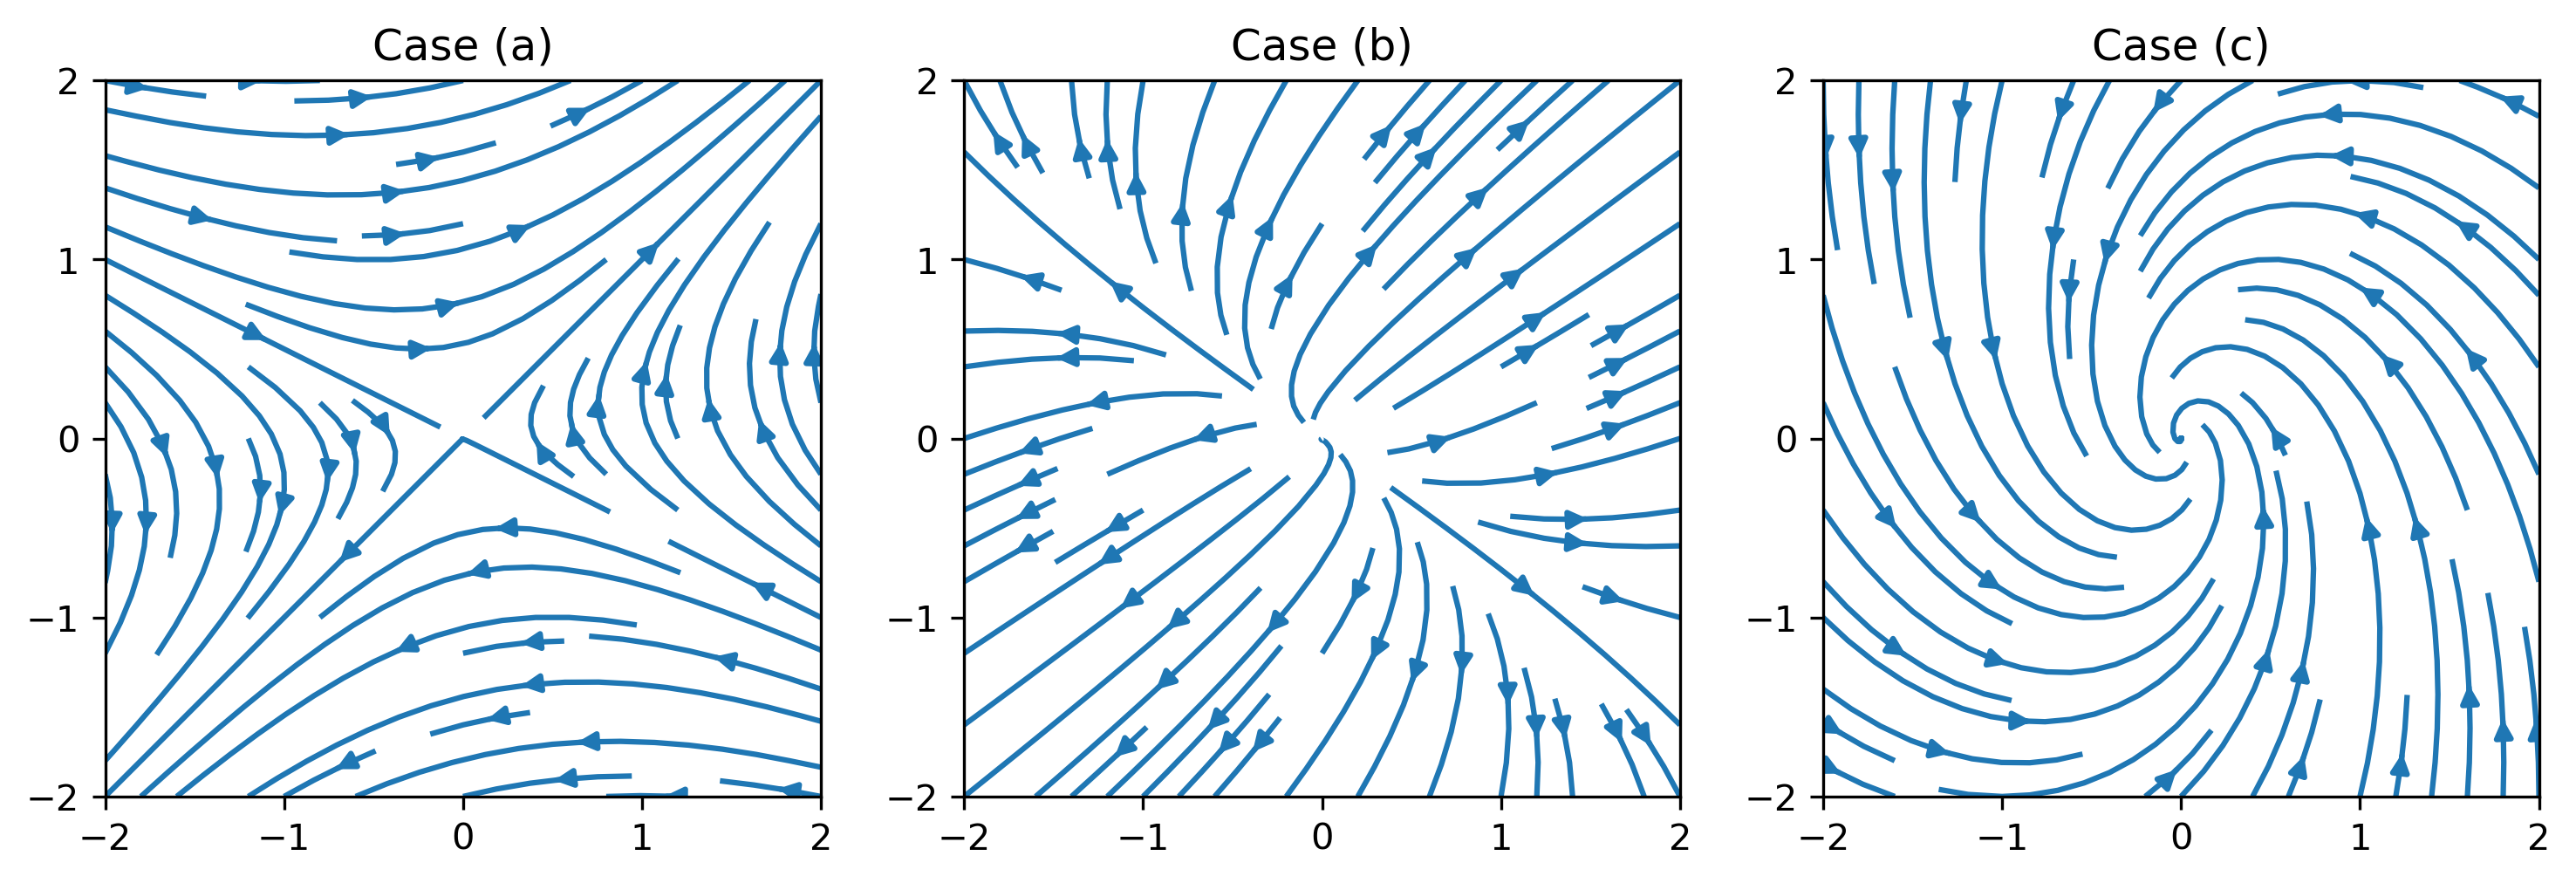
\includegraphics[width=\textwidth]{graphics/3exmps2ddynamic.png}
    \caption{\textit{The stream plots for the three two-dimensional dynamical systems in Example \ref{exmp:2d3dyn}.}}
    \label{fig:2d3dyn}
\end{figure}

\subsection{Generalization to Time-independent Forcings and Higher-dimensional Linear Dynamical Systems}

Sometimes there will be an additional forcing term on the R.H.S. of the linear dynamical system that represents external processes. Let's further assume that it is time-independent just like the dynamical system itself before so that we have
\begin{align}
\frac{d\textbf{y}}{dt} = A\textbf{y} + \textbf{G}
\end{align}
where $\textbf{G}$ is a constant vector with the same dimension as the state vector $\textbf{y}(t)$. As in Properties \ref{proper:2dequiltypes}, we require that $A$ is invertible, and hence by Theorem \ref{thm:sqlinsysunique} there exists a unique solution $\tilde{\textbf{y}}$ for the linear system $A\textbf{y} = -\textbf{G}$. Subsequently, the dynamical system can be rewritten into
\begin{align}
\frac{d\textbf{y}(t)}{dt} = A\textbf{y}(t) - A\tilde{\textbf{y}} = A(\textbf{y}(t) - \tilde{\textbf{y}})     
\end{align}
where a linear change of variable $\delta\textbf{y}(t) = \textbf{y}(t) - \tilde{\textbf{y}}$ will make it become
\begin{align}
\frac{d(\delta\textbf{y}(t))}{dt} = A(\delta\textbf{y}(t)) 
\label{eqn:translateddynsys}
\end{align}
which is essentially the same as (\ref{eqn:17.2}) but with $\delta\textbf{y}(t)$ in place of $\textbf{y}(t)$. Therefore, both the qualitative and quantitative behaviors of the dynamical system will also be the same except that the equilibrium point is now located by $\delta \textbf{y} = 0$, i.e.\ moved to $\textbf{y} = \tilde{\textbf{y}}$ instead of the original $\textbf{y} = \textbf{0}$. This effectively translates the equilibrium point and the entire corresponding phase portrait by a displacement of $\tilde{\textbf{y}}$, and the results from the previous discussion can thus be readily applied over linear dynamical systems with a time-independent forcing. Particularly, for a two-dimensional linear dynamical system as in (\ref{eqn:2ddynexplicit}), if we add an additional time-independent term so that it now looks like
\begin{align}
\left\{\begin{alignedat}{1}
\dfrac{dx}{dt} &= \beta_1^{(1)} x + \beta_2^{(1)} y + G_x \\
\dfrac{dy}{dt} &= \beta_1^{(2)} x + \beta_2^{(2)} y + G_y 
\end{alignedat}\right.
\end{align}
where $(G_x, G_y)^T = \textbf{G}$ are some fixed constants, and $\tilde{\textbf{y}} = (\tilde{x}, \tilde{y})^T$ is the unique solution to the linear system $A\textbf{y} = -\textbf{G}$ with $A$ in the form of (\ref{eqn:2ddynexplicit2}) and invertible such that
\begin{align}
\left\{\begin{alignedat}{1}
\beta_1^{(1)} \tilde{x} + \beta_2^{(1)} \tilde{y} &= -G_x \\
\beta_1^{(2)} \tilde{x} + \beta_2^{(2)} \tilde{y} &= -G_y 
\end{alignedat}\right.
\end{align}
then the dynamical system can be recast as
\begin{align}
&\left\{\begin{alignedat}{1}
\dfrac{dx}{dt} - \dfrac{d\tilde{x}}{dt} &= \beta_1^{(1)} x + \beta_2^{(1)} y - \beta_1^{(1)} \tilde{x} + \beta_2^{(1)} \tilde{y} \\
\dfrac{dy}{dt} - \dfrac{d\tilde{y}}{dt} &= \beta_1^{(2)} x + \beta_2^{(2)} y - \beta_1^{(2)} \tilde{x} + \beta_2^{(2)} \tilde{y} 
\end{alignedat}\right. \nonumber \\
&\left\{\begin{alignedat}{1}
\dfrac{d(x-\tilde{x})}{dt} &= \beta_1^{(1)} (x-\tilde{x}) + \beta_2^{(1)} (y-\tilde{y}) \\
\dfrac{d(y-\tilde{y})}{dt} &= \beta_1^{(2)} (x-\tilde{x}) + \beta_2^{(2)} (y-\tilde{y})
\end{alignedat}\right. \nonumber \\
\Rightarrow &\left\{\begin{alignedat}{1}
\dfrac{d(\delta x)}{dt} &= \beta_1^{(1)} \delta x + \beta_2^{(1)} \delta y \\
\dfrac{d(\delta y)}{dt} &= \beta_1^{(2)} \delta x + \beta_2^{(2)} \delta y
\end{alignedat}\right.
\label{eqn:2ddynfull}
\end{align}
which is essentially the same as (\ref{eqn:2ddynexplicit}) but with displacements from the newly translated equilibrium point $\delta x$ and $\delta y$ replacing the $x$ and $y$ coordinates that are initially relative to the origin.
\begin{exmp}
Locate the equilibrium point for the two-dimensional linear dynamical system
\begin{align*}
\left\{\begin{alignedat}{1}
\dfrac{dx}{dt} &= -5x + 2y + 8 \\
\dfrac{dy}{dt} &= x - 4y + 2
\end{alignedat}\right.
\end{align*}
and determined its type.
\end{exmp}
\begin{solution}
First, the position of the equilibrium point is found by solving the linear system
$A\textbf{y} = -\textbf{G}$ where
\begin{align*}
A &= 
\begin{bmatrix}
-5 & 2 \\
1 & -4
\end{bmatrix}
&
\textbf{G} &= 
\begin{bmatrix}
G_x \\
G_y
\end{bmatrix}
=
\begin{bmatrix}
8 \\
2
\end{bmatrix}
\end{align*}
It can be checked that the solution is
\begin{align*}
\tilde{\textbf{y}} = \begin{bmatrix}
2 \\
1
\end{bmatrix}
\end{align*}
as
\begin{align*}
\begin{bmatrix}
-5 & 2 \\
1 & -4
\end{bmatrix}
\begin{bmatrix}
2 \\
1
\end{bmatrix}
=
\begin{bmatrix}
-8 \\
-2
\end{bmatrix}
=
-\begin{bmatrix}
8 \\
2
\end{bmatrix}
\end{align*}
and thus the equilibrium point is at $\tilde{\textbf{y}} = (2,1)^T$. Next, translate the coordinate system so that it is now relative to this equilibrium point by writing $\delta x = x - 2$ and $\delta y = y - 1$. The dynamical system now looks like
\begin{align*}
&\left\{\begin{alignedat}{1}
\dfrac{d(x-2)}{dt} &= -5(x-2) + 2(y-1) \\
\dfrac{d(y-1)}{dt} &= (x-2) - 4(y-1)
\end{alignedat}\right. \\
&\left\{\begin{alignedat}{1}
\dfrac{d(\delta x)}{dt} &= -5\delta x + 2\delta y \\
\dfrac{d(\delta y)}{dt} &= \delta x - 4\delta y
\end{alignedat}\right.
\end{align*}
the one in (\ref{eqn:translateddynsys}) and the type of this equilibrium point can then be inferred from Table \ref{tab:equilpts}. The trace, determinant and discriminant are $\tr(A) = (-5) + (-4) = -9 < 0$, $\det(A) = (-5)(-4) - (1)(2) = 18 > 0$ and $\Delta = (-9)^2 - 4(18) = 9 > 0$, and therefore it is a stable node located at $(2,1)^T$.
\end{solution}

Another generalization to be made is for higher-dimensional dynamical systems. The logic in (\ref{eqn:eigendyn2d}) and Properties \ref{proper:2dequiltypes} remains the same. For a dynamical system $\textbf{y}' = A\textbf{y}$ of any dimension, let's say $n$, denote all the pair of eigenvalues and eigenvectors by $\lambda_j$ and $\smash{\vec{v}_\lambda^{(j)}}$, $j = 1, 2, \ldots, n$. Then the subspace spanned by those $\smash{\vec{v}_\lambda^{(j)}}$ with negative real $\lambda_j$ form the stable part of a node, and in contrast, those with positive real $\lambda_j$ form the unstable part of a node. If there are both stable and unstable parts, then they will give rise to an overall saddle point. The subspace spanned by a pair of $\smash{\vec{v}_\lambda^{(j)}}$ with the eigenvalues $\lambda_j$ being complex conjugates will lead to an unstable spiral if their real part is positive, a stable spiral if their real part is negative, and a center if it is exactly zero. The characteristic of the equilibrium point can be viewed either separately or together in these different subspaces (more formally known as \textit{"manifolds"} in this context).

\section{Non-linear Dynamical Systems}

\subsection{Heuristic Understandings of Stability and Attractiveness}
% https://math.stackexchange.com/questions/4453028/why-an-lti-system-with-some-zero-eigenvalues-still-stable
Before moving from linear dynamical systems to non-linear dynamical systems, we will take a detour to visit the concepts of stability and attractiveness. Heuristically, stability means that if the particle starts close enough to the equilibrium point, then it will always remain close to the equilibrium point. Meanwhile, attractiveness means that if it starts close enough to the equilibrium point likewise, then it will eventually be absorbed to that equilibrium point. We give the formal definitions for both of them below.
\begin{defn}
For a time-independent dynamical system as given by (\ref{eqn:eqpts1}) in Definition \ref{defn:eqpts}, an equilibrium point $\tilde{\textbf{y}}$ that satisfies (\ref{eqn:eqpts2}) is
\begin{enumerate}[label=(\alph*)]
    \item \index{Stable}\keywordhl{stable}, if for all $\epsilon > 0$, there exists an $\eta(\epsilon) > 0$\footnotemark{} such that $\norm{\textbf{y}(\textbf{y}_0, 0) - \tilde{\textbf{y}}} \leq \eta$ implies that $\norm{\textbf{y}(\textbf{y}_0, t) - \tilde{\textbf{y}}} \leq \epsilon$ for all $t \geq 0$;
    \item \index{Attractive}\keywordhl{attractive}, if there exists an $\eta > 0$ such that $\norm{\textbf{y}(\textbf{y}_0, 0) - \tilde{\textbf{y}}} \leq \eta$ implies that $\norm{\textbf{y}(\textbf{y}_0, t) - \tilde{\textbf{y}}} \to 0$ as $t \to \infty$.
\end{enumerate}
where $\textbf{y}(\textbf{y}_0, t)$ denotes the position of the particle at time $t$ with an initial condition (starting point) of $\textbf{y}_0 = \textbf{y}(\textbf{y}_0, 0)$. An equilibrium point is \index{Asymptotically Stable}\keywordhl{asymptotically stable} if it is both stable and attractive, and simply \index{Unstable}\keywordhl{unstable} if it is not stable.
\end{defn}
\footnotetext{Note that $\eta(\epsilon) \leq \epsilon$ implicitly. The definitions here and the following discussion are largely based on this \href{https://math.stackexchange.com/questions/4453028/why-an-lti-system-with-some-zero-eigenvalues-still-stable}{Math Stackexchange post} (4453028).} Translated to plain language, it means that the equilibrium point is stable if, for all particles starting inside a ball centered at the equilibrium point with a small radius of $\eta$, their subsequent trajectories will be contained within another ball with a small radius of $\epsilon$ at all times, whereas it is attractive if all particles starting inside some ball with a small radius of $\eta$ will converge to the equilibrium point as the time goes to infinity. It may be tempting to say that an attractive equilibrium point will be automatically (asymptotically) stable but there are some subtle differences between these two, demonstrated in the following counter-example. Consider the non-linear two-dimensional dynamical system
\begin{align}
&\left\{\begin{alignedat}{1}
\dfrac{dx}{dt} &= x^2 - y^2 \\
\dfrac{dy}{dt} &= 2xy
\end{alignedat}\right. 
\label{eqn:magneticdipolefield}
\end{align}
The pattern of its field lines is shown in Figure \ref{fig:magneticdipolefield}. 
\begin{figure}
    \centering
    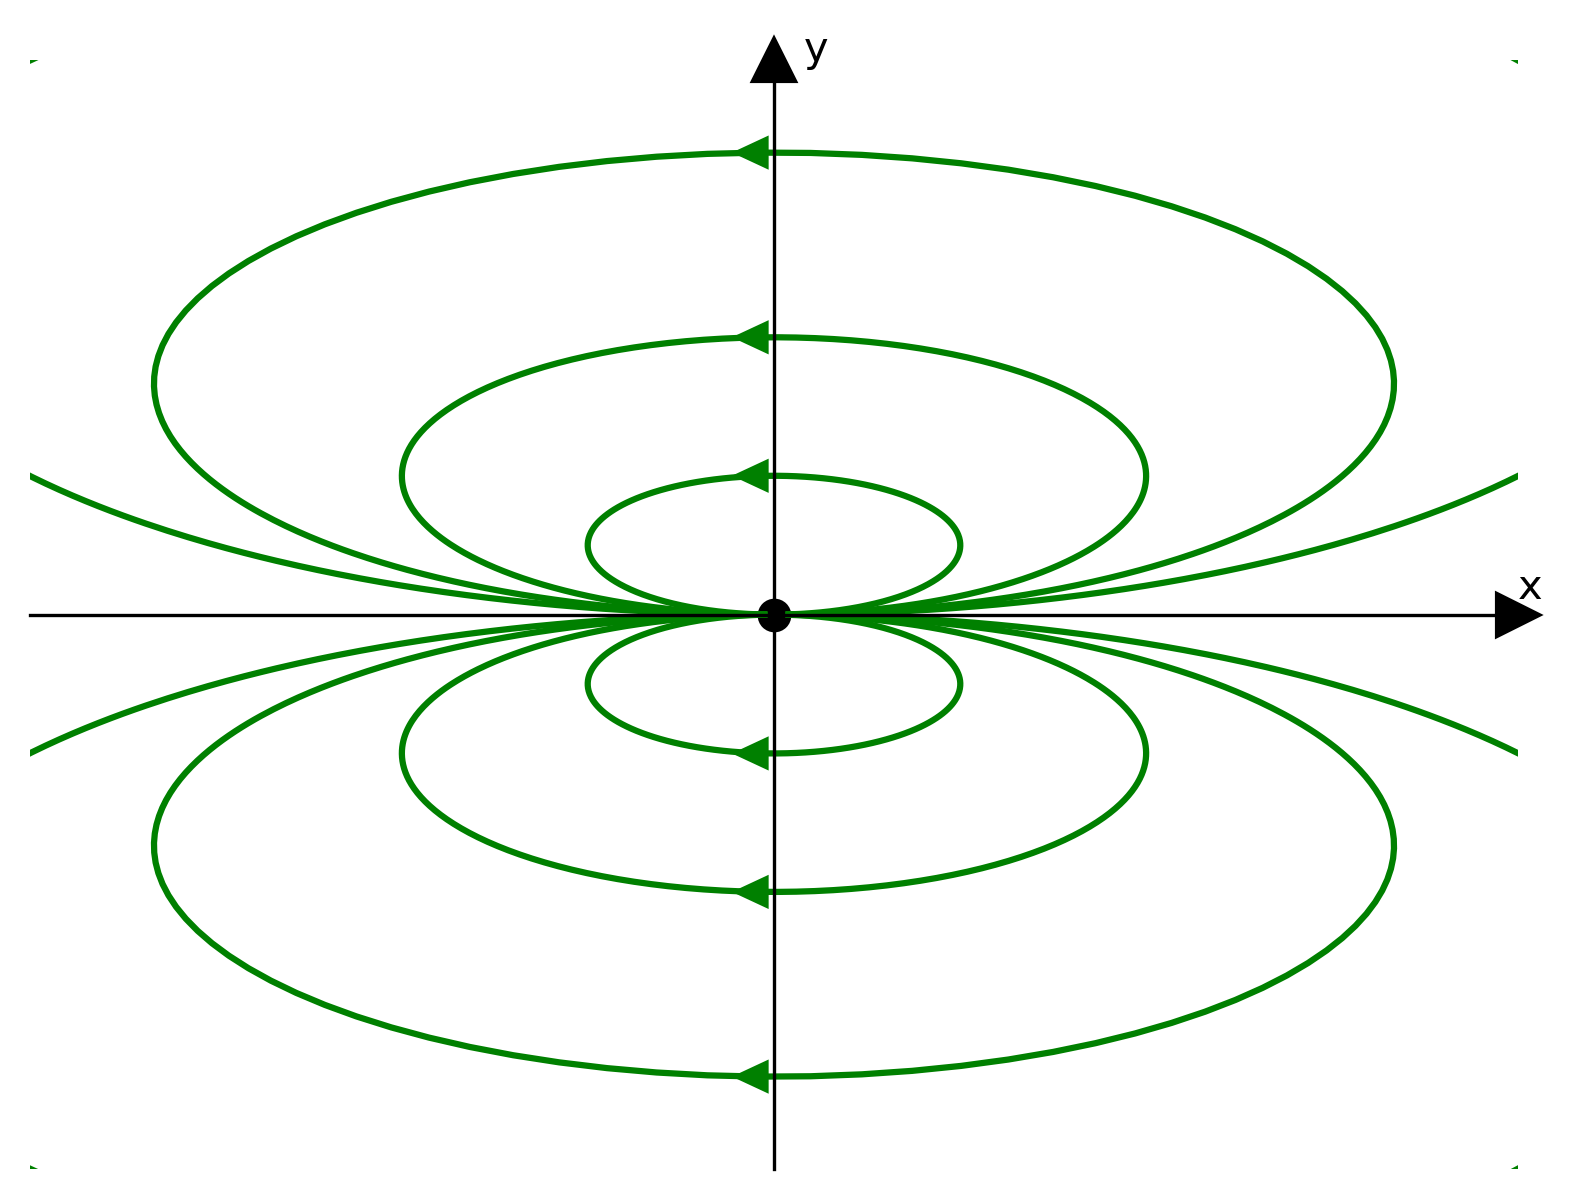
\includegraphics[scale=0.6]{graphics/dipolefield.png}
    \caption{\textit{Field lines for the non-linear dynamical system (\ref{eqn:magneticdipolefield}).}}
    \label{fig:magneticdipolefield}
\end{figure}
The field lines are akin to the \textit{magnetic dipole} type. The equilibrium point at the origin is attractive as all outgoing field lines will return to the equilibrium point, but is also unstable since we can always find a more outer field line that travels farther in both the $x$ and $y$-directions.\footnote{There is a caveat to this "counter-example" though. The "central" field line (not explicitly drawn out) that starts from $y = 0$ to the right of the equilibrium point will keep accelerating along the $x$-axis and diverges so it is only \textit{almost} attractive. In fact, it is impossible to have an unstable, yet \textit{truly} attractive equilibrium point if the dynamical system is smooth enough. However, the key takeaway is to help the readers distinguish between the concepts of stability and attractiveness, and this example should be adequate.} Nevertheless, all stable equilibrium types in Table \ref{tab:equilpts} except centers, are attractive and hence asymptotically stable.

\subsection{Linearization and Hartman-Grobman Theorem}
\label{subsection:HGthm}

Since non-linear dynamical systems are more complex, we may want to reduce them to the more familiar, linear dynamical systems. Motivated by the form (\ref{eqn:translateddynsys}), we seek to approximate the behavior of orbits near a non-linear equilibrium point by
\begin{align}
\frac{d(\delta y_i(t))}{dt} = \sum_{j=1}^{n} A_{ij}(\delta y_j (t)) = \sum_{j=1}^{n} \beta_{j}^{(i)}(\delta y_j(t)) \label{eqn:dynapproxproto}
\end{align}
where $\delta y_i$ represents a small displacement from the equilibrium point in the $i$-th direction, and each of the R.H.S. is a linear function of the displacement components with constant coefficients \smash{$\beta_{j}^{(i)}$}. Then, the previous (\ref{eqn:2ddynfull}) shows the fully written-out form of this approximation applicable to a two-dimensional dynamical system. Using Taylor Expansion to the first order from Multivariable Calculus, the non-linear dynamical system that takes the general form of (\ref{eqn:eqpts1}), or written in component form
\begin{align}
\frac{d y_i}{dt} = F_i(\textbf{y})
\end{align}
can be readily approximated by
\begin{align}
\frac{d(y_i(t) - \tilde{y}_i)}{dt} \approx F_i(\tilde{\textbf{y}}) + \sum_{j=1}^{n} \left(\left.\frac{\partial F_i}{\partial y_j}\right|_{\tilde{\textbf{y}}}\right) (y_j(t) - \tilde{y}_j) + O({\delta y_j}^2)
\end{align}
near the equilibrium point $\tilde{\textbf{y}}$ where \smash{$\partial F_i/\partial y_j|_{\tilde{\textbf{y}}}$} is the partial derivative of $F_i$ along the $j$-th direction evaluated at the equilibrium point. The matrix formed by \smash{$\partial F_i/\partial y_j$} is known as the \index{Jacobian (Matrix)}\keywordhl{Jacobian (matrix)}. Due to Definition \ref{defn:eqpts} of equilibrium points (\ref{eqn:eqpts2}), $F_i(\tilde{\textbf{y}}) = 0$, and if we further discard the higher-order error terms $O({\delta y_j}^2)$ it becomes
\begin{align}
\frac{d(\delta y_i(t))}{dt} = \sum_{j=1}^{n}  \left(\left.\frac{\partial F_i}{\partial y_j}\right|_{\tilde{\textbf{y}}}\right) \delta y_j(t) \label{eqn:nonlindynjac}
\end{align}
Comparing with the proposed form in (\ref{eqn:dynapproxproto}), we immediately identity the required coefficients \smash{$\beta_{j}^{(i)}$} with \smash{$\partial F_i/\partial y_j|_{\tilde{\textbf{y}}}$}. For a two-dimensional non-linear dynamical system, the corresponding fully written-out form is then
\begin{align}
&\left\{\begin{alignedat}{1}
\dfrac{d(\delta x)}{dt} &= \dfrac{\partial F_1}{\partial x}(\tilde{x}, \tilde{y}) \delta x + \dfrac{\partial F_1}{\partial y}(\tilde{x}, \tilde{y}) \delta y \\
\dfrac{d(\delta y)}{dt} &= \dfrac{\partial F_2}{\partial x}(\tilde{x}, \tilde{y}) \delta x + \dfrac{\partial F_2}{\partial y}(\tilde{x}, \tilde{y}) \delta y
\end{alignedat}\right.
\end{align}
Now, the problem is whether such a \index{Linearization}\keywordhl{linearization} of the non-linear equilibrium point can successfully capture its characteristics. To proceed, we first introduce a class of equilibrium points known as \index{Hyperbolic Equilibrium Point}\keywordhl{hyperbolic equilibrium points}.
\begin{defn}[Hyperbolic Equilibrium Points]
For a linear dynamical system as formulated by (\ref{eqn:translateddynsys}), 
a hyperbolic equilibrium point is an equilibrium point where all the eigenvalues of $A$ have non-zero real parts. Similarly, for a non-linear dynamical system, a hyperbolic equilibrium point is an equilibrium point where all the eigenvalues of the Jacobian matrix $A_{ij} = \smash{\partial F_i/\partial y_j|_{\tilde{\textbf{y}}}}$ in the linearization by (\ref{eqn:nonlindynjac}) have non-zero real parts, evaluated at the equilibrium point.
\end{defn}
By this criteria, in Table \ref{tab:equilpts}, the stable/unstable nodes, saddle points, and stable/unstable spirals are all hyperbolic equilibrium points. The only exception is the centers, in addition to other omitted degenerate cases where at least one of the eigenvalues is strictly zero. Since stable equilibrium types excluding centers are all asymptotically stable as noted at the end of the last subsection, hyperbolic equilibrium points are either asymptotically stable or unstable. Now we are ready to examine the major result about hyperbolic equilibrium points, the \index{Hartman-Grobman Theorem}\keywordhl{Hartman-Grobman (Linearization) Theorem}, which states that the qualitative behavior of orbits near a non-linear hyperbolic equilibrium point will be the same as its linearization.
\begin{thm}[Hartman-Grobman Theorem]
\label{thm:HGthm}
A hyperbolic equilibrium point $\tilde{\textbf{y}}$ of any non-linear dynamical system that has a Jacobian of $\smash{\partial F_i/\partial y_j|_{\tilde{\textbf{y}}}}$, belongs to the same type and has the same qualitative behavior in its neighborhood as the corresponding linear hyperbolic equilibrium point, with the matrix $A$ in (\ref{eqn:translateddynsys}) equal to this Jacobian $\smash{\partial F_i/\partial y_j|_{\tilde{\textbf{y}}}}$.
\end{thm}
Unfortunately, for an equilibrium point that is not hyperbolic, we need other methods to determine its behavior which are out of the scope of this book. Anyway, let's see how the Hartman-Grobman Theorem can be applied in the following example.
\begin{exmp}
\label{exmp:nonlindynsaddlenode}
Find all the equilibrium points for the two-dimensional non-linear dynamical system
\begin{align*}
\left\{
\begin{aligned}
\frac{dx}{dt} &= y - xy \\
\frac{dy}{dt} &= x - xy
\end{aligned}
\right.
\end{align*}
\end{exmp}
\begin{solution}
Since the dynamical system is now non-linear we can have multiple isolated equilibrium points. A simple rewriting of the dynamical system shows that
\begin{align*}
\left\{
\begin{aligned}
\frac{dx}{dt} &= y (1-x) \\
\frac{dy}{dt} &= x (1-y)
\end{aligned}
\right.
\end{align*}
from which we can easily deduce the two equilibrium points: $(\tilde{x}, \tilde{y}) = (0,0)$ or $(1,1)$. The Jacobian of the non-linear dynamical system is
\begin{align*}
\dfrac{\partial F_i}{\partial y_j} &= 
\begin{bmatrix}
\dfrac{\partial F_1}{\partial x} & \dfrac{\partial F_1}{\partial y} \\[10pt]
\dfrac{\partial F_2}{\partial x} & \dfrac{\partial F_2}{\partial y}
\end{bmatrix} \\
&= 
\begin{bmatrix}
\dfrac{\partial (y-xy)}{\partial x} & \dfrac{\partial (y-xy)}{\partial y} \\[10pt]
\dfrac{\partial (x-xy)}{\partial x} & \dfrac{\partial (x-xy)}{\partial y}
\end{bmatrix} \\
&= 
\begin{bmatrix}
-y & 1-x \\
1-y & -x
\end{bmatrix}
\end{align*}
At the first equilibrium point $(\tilde{x}, \tilde{y}) = (0,0)$, the Jacobian is
\begin{align*}
\left.\dfrac{\partial F_i}{\partial y_j}\right|_{(0,0)} &= 
\begin{bmatrix}
0 & 1 \\
1 & 0
\end{bmatrix}
\end{align*}
the characteristic polynomial of which is simply $\lambda^2 - 1 = (\lambda - 1)(\lambda + 1)$ and thus it has two eigenvalues of $-1$ and $1$, one positive and one negative. By the Hartman-Grobman Theorem, this means that the first equilibrium point $(\tilde{x}, \tilde{y}) = (0,0)$ is locally a saddle point. On the other hand, at the second equilibrium point $(\tilde{x}, \tilde{y}) = (1,1)$, the Jacobian is
\begin{align*}
\left.\dfrac{\partial F_i}{\partial y_j}\right|_{(1,1)} &= 
\begin{bmatrix}
-1 & 0 \\
0 & -1
\end{bmatrix}
\end{align*}
which clearly has a repeated negative eigenvalue of $-1$ with a multiplicity of $2$, and thus by the Hartman-Grobman Theorem it is locally a sink (stable node). The phase portrait of this dynamical system is shown in Figure \ref{fig:nonlinearphase}.
\end{solution}
\begin{figure}[ht!]
    \centering
    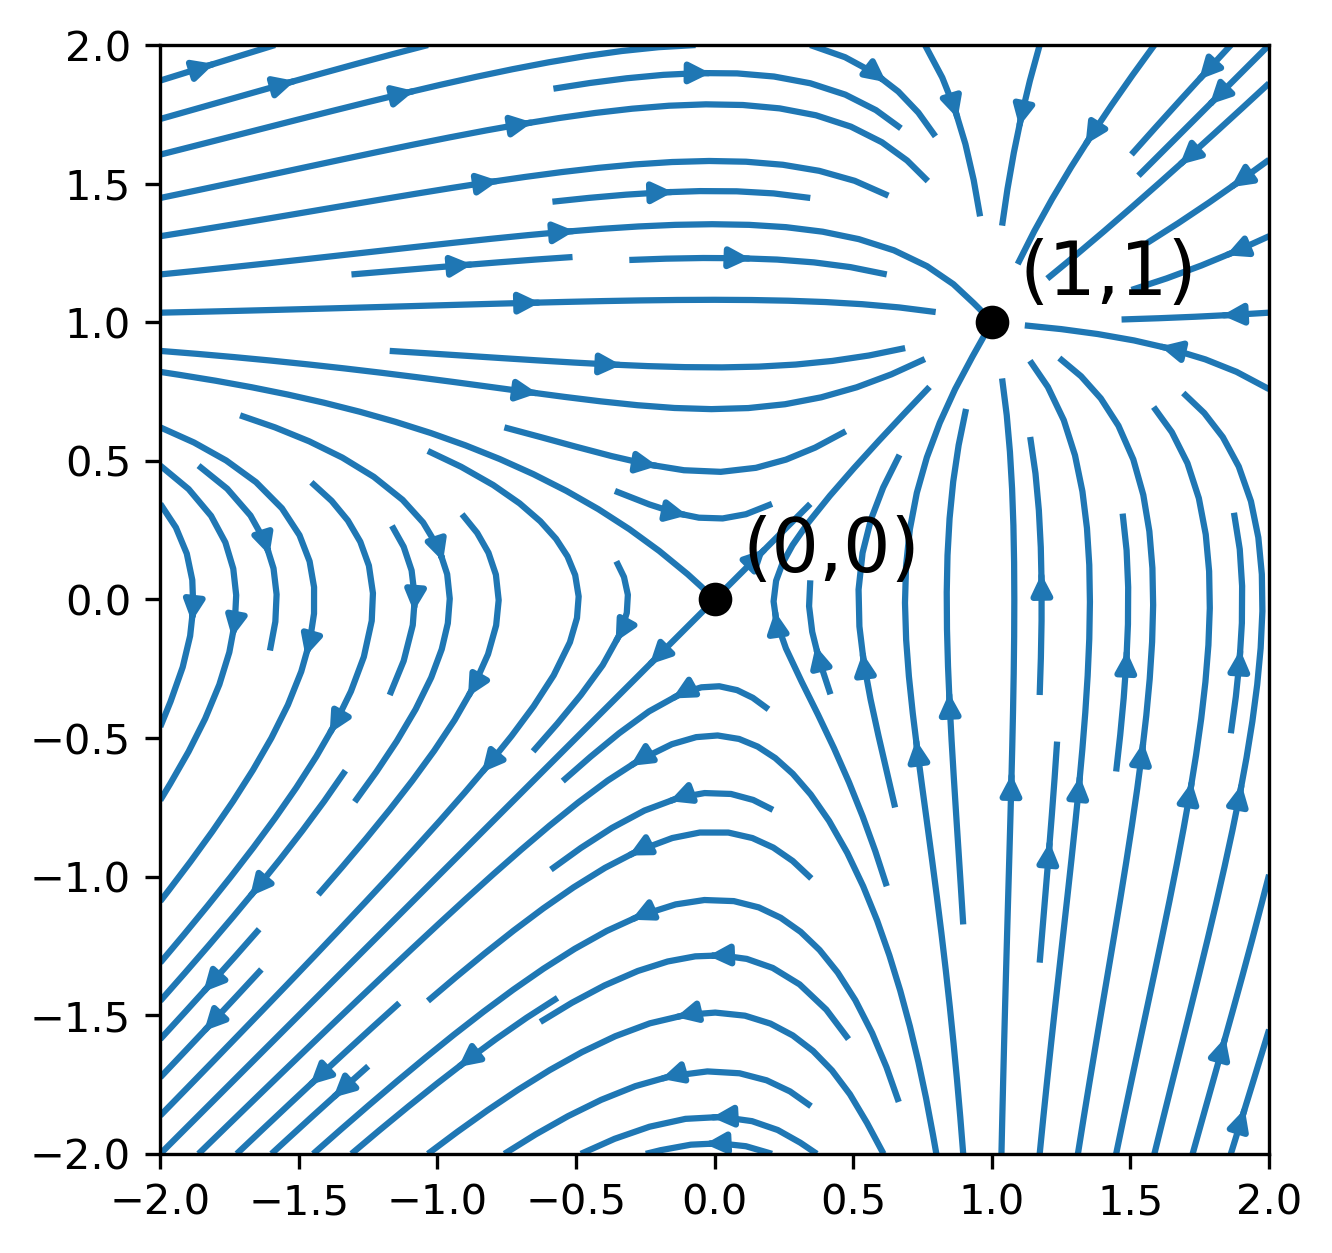
\includegraphics[scale=0.7]{graphics/saddlenode.png}
    \caption{\textit{The stream plot for the dynamical system in Example \ref{exmp:nonlindynsaddlenode}.}}
    \label{fig:nonlinearphase}
\end{figure}

\section{Earth Science Applications: the Lorenz-63 Model}

The \index{Lorenz-63 Model}\keywordhl{Lorenz-63 Model} is consisted of three variables $X,Y,Z$ and their evolutions in time are described by
\begin{subequations}
\label{eqn:lor63f}
\begin{empheq}[left={\empheqlbrace}]{alignat=1}
\frac{dX}{dt} &= -\sigma X + \sigma Y \label{eqn:lor63a} \\ 
\frac{dY}{dt} &= -XZ + \rho X - Y \label{eqn:lor63b} \\
\frac{dZ}{dt} &= XY - \beta Z \label{eqn:lor63c}
\end{empheq}
\end{subequations}
where the parameters $\sigma, \rho, \beta > 0$ are all positive. It is a minimalist model that demonstrates the phenomenon of \textit{chaos}. In the following subsections, we will discuss the context in which the model is formulated and the characteristics of its equilibrium points.

\subsection{Derivation of the Lorenz-63 Model}

\textit{Reference Materials: \cite{kaic}}

The Lorenz-63 model originates from a simplified version of the \textit{Rayleigh-Barnard Convection} Problem about the convective/diffusion-driven flow. Particularly, we will restrict ourselves to a two-dimensional flow in the $x$/$z$-(zonal/meridional) directions so that the velocity vector is $\vec{u} = (u_x, 0, u_z)^T$. The governing equations for this scenario are the zonal/meridional \textit{momentum equations}, \textit{thermodynamics equation}, and the \textit{continuity equation} with \textit{Boussinesq approximation} as follows. \begin{empheq}[left={\empheqlbrace}]{alignat=2}
& \frac{\partial u_x}{\partial t} + u_x\frac{\partial u_x}{\partial x} + u_z \frac{\partial u_x}{\partial z} & &= \nu(\frac{\partial^2 u_x}{\partial x^2} + \frac{\partial^2 u_x}{\partial z^2}) - \frac{1}{\rho_0} \frac{\partial p}{\partial x} \label{eqn:RB1} \\
&\frac{\partial u_z}{\partial t} + u_x\frac{\partial u_z}{\partial x} + u_z \frac{\partial u_z}{\partial z} & &= \nu(\frac{\partial^2 u_z}{\partial x^2} + \frac{\partial^2 u_z}{\partial z^2}) - \frac{1}{\rho_0} \frac{\partial p}{\partial z} + \alpha T g \label{eqn:RB2} \\
&\frac{\partial T}{\partial t} - u_z\Gamma + u_x\frac{\partial T}{\partial x} + u_z\frac{\partial T}{\partial z} & &= \kappa (\frac{\partial^2 T}{\partial x^2} + \frac{\partial^2 T}{\partial z^2})  \label{eqn:RB3} \\
& \frac{\partial u_x}{\partial x} + \frac{\partial u_z}{\partial z} & &= 0 \label{eqn:RB4}
\end{empheq}
The constants are: $g$, the gravitational acceleration; $\alpha$, the thermal expansion coefficient of the fluid; the lapse rate $\Gamma = -\frac{T_L - T_H}{d}$ which is the difference in the temperature prescribed at the top and bottom plates over the vertical depth of the fluid $d$; $\rho_0$, the reference fluid density; $\nu$ and $\kappa$, the kinematic viscosity and thermal diffusivity. In addition to the velocities $u_x$ and $u_z$, there are two other variables: $T$ as the departure of temperature from the reference profile and $p$ as the pressure perturbation. By the \index{Buckingham Pi Theorem}\keywordhl{Buckingham Pi Theorem}\footnote{It states that all physically consistent laws are "unit-independent" and the number of non-dimensional variables required to transform a set of equations into dimensionless form is the number of physical variables minus the number of fundamental physical dimensions. There are $13$ physical variables here, time $t$, two displacements $x$ and $z$, two velocities $u_x$ and $u_z$, temperature $T$, kinematic viscosity $\kappa$, thermal diffusivity $\nu$, pressure $p$, density $\rho_0$, thermal expansion coefficient $\alpha$ and gravity $g$ (together counted as a single variable as they appear in the equation once and only once in combination over the term $\alpha Tg$), and finally two other variables, the vertical depth $d$ and temperature difference $T_L-T_H$, derived from lapse rate $\Gamma$. Meanwhile, there are $4$ fundamental dimensions: length, time, mass, and temperature. So there will be $13 - 4 = 9$ non-dimensional variables.}, we can convert these equations into dimensionless form using $9$ non-dimensional variables:
\begin{subequations}
\begin{empheq}[left={\empheqlbrace}]{alignat=2}
&x^* & &= \frac{x}{d}\\
&z^* & &= \frac{z}{d}\\
&t^* & &= \frac{t}{d^2/\kappa}\\
&u_x^* & &= \frac{u_x}{\kappa/d}\\
&u_z^* & &= \frac{u_z}{\kappa/d}\\
&T^* & &= \frac{T}{\kappa\nu/g\alpha d^3}\\
&p^* & &= \frac{p}{\rho_0\kappa^2/d^2}\\
&\sigma & &= \frac{\nu}{\kappa}\\
&R & &= \frac{g\alpha d^3(T_H-T_L)}{\kappa\nu}
\end{empheq}
\end{subequations}
The first $7$ of them are the non-dimensional (indicated by the asterisk $^*$) physical variables of displacements, time, velocities, temperature, and pressure with the characteristic length/time/velocity/temperature/pressure scales of $d$, $d^2/\kappa$ (the \textit{dissipation timescale}), $\kappa/d$, $\kappa\nu/g\alpha d^3$, and $\rho_0\kappa^2/d^2$. The last two of them are the \textit{Prandlt number} $\sigma = \frac{\nu}{\kappa}$ as the ratio of thermal diffusivity $\nu$ to kinematic viscosity $\kappa$, and \textit{Rayleigh number} \smash{$R = \frac{g\alpha d^3(T_H-T_L)}{\kappa\nu}$}. As we will see later, these two parameters will decide the behavior of the system. By substituting all these into (\ref{eqn:RB1}), we have
\begin{align*}
&\quad \left(\frac{\kappa/d}{d^2/\kappa}\right)\frac{\partial u_x^*}{\partial t^*} + \left(\frac{(\kappa/d)^2}{d}\right)u_x^*\frac{\partial u_x^*}{\partial x^*} + \left(\frac{(\kappa/d)^2}{d}\right)u_z^* \frac{\partial u_x^*}{\partial z^*} \\
&= \nu\left(\left(\frac{\kappa/d}{d^2}\right)\frac{\partial^2 u_x^*}{\partial {x^*}^2} + \left(\frac{\kappa/d}{d^2}\right)\frac{\partial^2 u_x^*}{\partial {z^*}^2}\right) - \left(\frac{\kappa^2/d^2}{d}\right)\frac{\partial p^*}{\partial x^*}    
\end{align*}
Dividing both sides of the equation by the factor \smash{$\frac{\kappa^2}{d^3}$} leads to
\begin{align}
\frac{\partial u_x^*}{\partial t^*} + u_x^*\frac{\partial u_x^*}{\partial x^*} + u_z^* \frac{\partial u_x^*}{\partial z^*} 
&= \frac{\nu}{\kappa}\left(\frac{\partial^2 u_x^*}{\partial {x^*}^2} + \frac{\partial^2 u_x^*}{\partial {z^*}^2}\right) - \frac{\partial p^*}{\partial x^*} \nonumber \\
&= \sigma\left(\frac{\partial^2 u_x^*}{\partial {x^*}^2} + \frac{\partial^2 u_x^*}{\partial {z^*}^2}\right) - \frac{\partial p^*}{\partial x^*} \label{eqn:RB1n}
\end{align}
Similarly, by noticing that $\alpha T g = \frac{\kappa\nu}{d^3} T^*$, we can rewrite (\ref{eqn:RB2}) into
\begin{align}
\frac{\partial u_z^*}{\partial t^*} + u_x^*\frac{\partial u_z^*}{\partial x^*} + u_z^* \frac{\partial u_z^*}{\partial z^*} &= \sigma\left(\frac{\partial^2 u_z^*}{\partial {x^*}^2} + \frac{\partial^2 u_z^*}{\partial {z^*}^2}\right) - \frac{\partial p^*}{\partial z^*} + \sigma T^* \label{eqn:RB2n}
\end{align}
Meanwhile, (\ref{eqn:RB3}) can be transformed into
\begin{align*}
&\quad \left(\frac{\kappa\nu/g\alpha d^3}{d^2/\kappa}\right)\frac{\partial T^*}{\partial t^*} + (\kappa/d)u_z^* \left(\frac{T_L - T_H}{d}\right) \\
&\quad + \left(\frac{(\kappa/d)(\kappa\nu/g\alpha d^3)}{d}\right)u_x^*\frac{\partial T^*}{\partial x^*} + \left(\frac{(\kappa/d)(\kappa\nu/g\alpha d^3)}{d}\right)u_z^*\frac{\partial T^*}{\partial z^*} \\
&= \kappa \left(\left(\frac{\kappa\nu/g\alpha d^3}{d^2}\right)\frac{\partial^2 T^*}{\partial {x^*}^2} + \left(\frac{\kappa\nu/g\alpha d^3}{d^2}\right)\frac{\partial^2 T^*}{\partial {z^*}^2}\right)  
\end{align*}
This time, dividing by the factor \smash{$\frac{\kappa^2\nu}{g\alpha d^5}$} gives
\begin{align}
&\quad \frac{\partial T^*}{\partial t^*} + u_z^* \left(\frac{g\alpha d^3(T_L - T_H)}{\kappa\nu}\right) + u_x^*\frac{\partial T^*}{\partial x^*} + u_z^*\frac{\partial T^*}{\partial z^*} \nonumber \\
&= \frac{\partial T^*}{\partial t^*} + R u_z^* + u_x^*\frac{\partial T^*}{\partial x^*} + u_z^*\frac{\partial T^*}{\partial z^*} = \frac{\partial^2 T^*}{\partial {x^*}^2} + \frac{\partial^2 T^*}{\partial {z^*}^2} \label{eqn:RB3n}
\end{align}
Finally, the non-dimensional form of the mass continuity equation (\ref{eqn:RB4}) is simply
\begin{align}
\frac{\partial u_x^*}{\partial x^*} + \frac{\partial u_z^*}{\partial z^*} &= 0 \label{eqn:loreznmasscont}
\end{align}
According to this, we can rewrite $\vec{u}^* = (u_x^*, 0, u_z^*)^T = (-\frac{\partial \psi^*}{\partial z^*}, 0, \frac{\partial \psi^*}{\partial x^*})$ where $\psi^*$ is known as the (non-dimensional) \index{Stream Function}\keywordhl{stream function}. This is possible as the problem is set up to be two-dimensional and we will further require it to be bounded, such that $\vec{u} = \textbf{0}$ and $T = 0$ ($\vec{u}^* = \textbf{0}$ and $T^* = 0$) at $z = 0,d$ ($z^* = 0,1$) and the boundary condition along the $x$-direction is periodic. With
\begin{subequations}
\label{eqn:lorenzstreamv}
\begin{empheq}[left={\empheqlbrace}]{alignat=1}
u_x^* &= -\frac{\partial \psi^*}{\partial z^*} \\
u_z^* &= \frac{\partial \psi^*}{\partial x^*}
\end{empheq}
\end{subequations}
(\ref{eqn:loreznmasscont}) is then automatically satisfied.\footnote{$\frac{\partial u_x^*}{\partial x^*} + \frac{\partial u_z^*}{\partial z^*} = -\frac{\partial \psi^*}{\partial x^*\partial z^*} + \frac{\partial \psi^*}{\partial x^*\partial z^*} \equiv 0$.} Now substituting (\ref{eqn:lorenzstreamv}) into (\ref{eqn:RB1n}) and (\ref{eqn:RB2n}), and writing $\frac{\partial}{\partial[\;]} = \partial_{[\;]}$ for simplicity, we have
\begin{align}
&\quad \partial_{t^*} \partial_{z^*} \psi^* - (\partial_{z^*} \psi^*)(\partial_{x^*} \partial_{z^*} \psi^*) + (\partial_{x^*} \psi^*) ((\partial_{z^*})^2 \psi^*) \nonumber \\
&= \sigma\left((\partial_{x^*})^2\partial_{z^*} \psi^* + (\partial_{z^*})^3 \psi^* \right) + \partial_{x^*} p^* \label{eqn:RBpsia}
\end{align}
and
\begin{align}
&\quad \partial_{t^*} \partial_{x^*} \psi^* - (\partial_{z^*} \psi^*)((\partial_{x^*})^2 \psi^*) + (\partial_{x^*} \psi^*) (\partial_{z^*} \partial_{x^*} \psi^*) \nonumber \\
&= \sigma\left((\partial_{x^*})^3 \psi^* + (\partial_{z^*})^2 \partial_{x^*} \psi^* \right) - \partial_{z^*} p^* + \sigma T^* \label{eqn:RBpsib}
\end{align}
Differentiating (\ref{eqn:RBpsia}) with respect to $z$ and (\ref{eqn:RBpsib}) with respect to $x$, and then adding them together will eliminate the pressure term and lead to an L.H.S. of
\begin{align*}
&\quad [\partial_{t^*}  (\partial_{z^*} )^2 \psi^* \mathcolor{red}{-((\partial_{z^*} )^2 \psi^*)(\partial_{x^*}  \partial_{z^*}  \psi^*)}  - (\partial_{z^*}  \psi^*)(\partial_{x^*}  (\partial_{z^*} )^2 \psi^*) \\
&\quad \mathcolor{red}{+ (\partial_{z^*}  \partial_{x^*}  \psi^*) ((\partial_{z^*} )^2 \psi^*)} + (\partial_{x^*}  \psi^*) ((\partial_{z^*} )^3 \psi^*)] \\
&\quad + [\partial_{t^*}  (\partial_{x^*} )^2 \psi^* \mathcolor{red}{- (\partial_{x^*} \partial_{z^*}  \psi^*)((\partial_{x^*} )^2 \psi^*)} - (\partial_{z^*}  \psi^*)((\partial_{x^*} )^3 \psi^*) \\
&\quad \mathcolor{red}{+ ((\partial_{x^*} )^2 \psi^*) (\partial_{z^*}  \partial_{x^*}  \psi^*)} + (\partial_{x^*}  \psi^*) (\partial_{z^*}  (\partial_{x^*} )^2 \psi^*)] \\
&= \partial_{t^*}  ((\partial_{x^*} )^2 + (\partial_{z^*} )^2) \psi^* - (\partial_{z^*} \psi^*) (\partial_{x^*}  ((\partial_{x^*})^2 + (\partial_{z^*})^2)\psi^*) \\
&\quad + (\partial_{x^*} \psi^*) (\partial_{z^*}  ((\partial_{x^*})^2 + (\partial_{z^*})^2)\psi^*) 
\end{align*}
and an R.H.S. of
\begin{align*}
&\quad [\sigma\left((\partial_{x^*})^2(\partial_{z^*})^2 \psi^* + (\partial_{z^*})^4 \psi^* \right) \mathcolor{red}{+ \partial_{z^*} \partial_{x^*} p^*}] \\
&\quad + [\sigma\left((\partial_{x^*})^4 \psi^* + (\partial_{z^*})^2 (\partial_{x^*})^2 \psi^* \right) \mathcolor{red}{- \partial_{x^*} \partial_{z^*} p^*} + \sigma \partial_{x^*} T^*] \\
&= \sigma ((\partial_{x^*})^2 + (\partial_{z^*})^2)^2 \psi^* + \sigma \partial_{x^*} T^*
\end{align*}
By using the \textit{Laplacian} symbol $\Delta^* = (\partial_{x^*})^2 + (\partial_{z^*})^2$ in this equation, and also substituting the stream function (\ref{eqn:lorenzstreamv}) into the other equation (\ref{eqn:RB3n}), we can sort out a set of two equations in two unknowns $\psi^*$ and $T^*$, that describes the evolution of the system state:
\begin{empheq}[left={\empheqlbrace}]{alignat=1}
\partial_{t^*} \Delta^* \psi^* - (\partial_{z^*} \psi^*) (\partial_{x^*}\Delta^* \psi^*) + (\partial_{x^*} \psi^*) (\partial_{z^*}\Delta^* \psi^*) &= \sigma {\Delta^*}^2\psi^* + \mathrlap{\sigma \partial_{x^*} T^*} \label{eqn:lorenzwind} \\
\partial_{t^*}T^* - (\partial_{z^*} \psi^*)(\partial_{x^*} T^*) + (\partial_{x^*} \psi^*)(\partial_{z^*} T^*) &= \Delta^* T^* - R \partial_{x^*} \psi^* \label{eqn:lorenztemp}
\end{empheq} As mentioned before, the statistics of the system are controlled by the two parameters $\sigma$ and $R$ here. However, we still have to simplify the problem to make it tractable while retaining the chaotic nature. For this, we will decompose the variables $T^*$ and $\psi^*$ into Fourier modes along the zonal and meridional directions. Since the boundary conditions are periodic and fixed to zero in the $x$ and $z$-directions respectively, we assume that the solution will take the following form of infinite summations of basis functions in terms of products between complex exponentials and sines (can refer to Section \ref{section:DFT}):
\begin{subequations}
\begin{empheq}[left={\empheqlbrace}]{alignat=1}
T^*(x^*,z^*,t^*) &= \sum_{k_1 = -\infty}^{\infty} \sum_{k_2 = 1}^{\infty} \hat{T}_{k_1,k_2}(t^*) e^{ik_1\pi a x^*} \sin(k_2\pi z^*) \\
\psi^*(x^*,z^*,t^*) &= \sum_{k_1 = -\infty}^{\infty} \sum_{k_2 = 1}^{\infty} \hat{\psi}_{k_1,k_2}(t^*) e^{ik_1\pi a x^*} \sin(k_2\pi z^*)
\end{empheq}     
\end{subequations}
where $a = d/l$ is the aspect ratio (depth to width) of the domain\footnote{$\frac{z}{d} = z^*$, $\frac{x}{l} = \frac{dx^*}{l} = ax^*$.}. To proceed, we first need to understand that to generate various Fourier basis functions with new wave numbers, we have to rely on the non-linearity due to the interaction of flow with different wave numbers (scales). Otherwise, the orthogonality of the Fourier modes will prevent this from happening over linear terms. Heuristically, if we look at, for example, the portion of the complex exponentials in $x^*$ for two $\psi^*$ basis functions, \smash{$\hat{\psi}_{k} e^{ik\pi a x^*}$} and \smash{$\hat{\psi}_{l} e^{il\pi a x^*}$}, then their product (as well as with one of them conjugated) will produce
\begin{subequations}
\label{eqn:nonlinearinter}
\begin{empheq}[left={\empheqlbrace}]{alignat=1}
\psi^*_k\psi^*_l &= \hat{\psi}_{k}\hat{\psi}_{l} e^{i(k+l)\pi a x^*} \\
\psi^*_k\overline{\psi^*_l} &= \hat{\psi}_{k}\overline{\hat{\psi}_{l}} e^{i(k-l)\pi a x^*}
\end{empheq} 
\end{subequations}
So the new signal can have either a wave number of $k + l$ and $k - l$. If particularly one of the original wave numbers $k$ and $l$ is $1$, then by inductively using this property we can essentially generate all wave numbers and hence the full dynamics. Therefore, we are motivated to focus on the Fourier modes with a wave number of $1$. Again we will first look at the $x^*$ portion of the Fourier modes and we will choose the imaginary part of $\hat{\psi}_{k_1 = 1}$ which is $\hat{\psi}_{k_1 = 1} \sin(\pi a x^*)$ as the starting point. We will drop the non-linear advection term $- (\partial_{z^*} \psi^*) (\partial_{x^*}\Delta^* \psi^*) + (\partial_{x^*} \psi^*) (\partial_{z^*}\Delta^* \psi^*)$ in the prognostic equation (\ref{eqn:lorenzwind}) of $\psi^*$ to trim down the model. This makes the $\sigma \partial_{x^*} T^*$ term on R.H.S. become the only way to keep the non-linearity (the remaining $\sigma {\Delta^*}^2\psi^*$ is only a linear damping term). For this $\sigma \partial_{x^*} T^*$ term to contribute to the tendency of $\hat{\psi}_{k_1 = 1} \sin(\pi a x^*)$ in the time derivative term $\partial_{t^*} \Delta^* \psi^*$ on L.H.S., we must also have the real part of $\hat{T}_{k_1 = 1}$ which is $\hat{T}_{k_1 = 1} \cos(\pi a x^*)$, due to the form of $\sigma \partial_{x^*} T^*$ which upon substitution becomes $-\sigma \pi a \hat{T}_{k_1 = 1} \sin(\pi a x^*)$, so that it is compatible with the sine part of $\hat{\psi}_{k_1 = 1} \sin(\pi a x^*)$ with a wave number of $1$. \par

Since we have removed the advection term in the prognostic equation of $\psi^*$, we have to keep the advection term $- (\partial_{z^*} \psi^*)(\partial_{x^*} T^*) + (\partial_{x^*} \psi^*)(\partial_{z^*} T^*)$ in the prognostic equation of $T^*$ to ensure the non-linearity of the whole dynamical system. By the previous argument over (\ref{eqn:nonlinearinter}), as long as either the sum of or difference in wave numbers $k_1$ and $k_2$ between the two scales is $1$ ($k_1 + k_2 = 1$ or $k_1 - k_2 = 1$), then their non-linear interaction can generate the required wave number $1$ signal (the real part of $\hat{T}_{k_1 = 1}$). One of the simplest ways to achieve this without involving too many new scales is to introduce the real part of the mean temperature $\hat{T}_{k_1 = 0}$ which is a constant in $x^*$, so that the forcing term for $\hat{T}_{k_1 = 1} \cos(\pi ax^*)$ is produced in (\ref{eqn:lorenztemp}) as we already have $\hat{\psi}_{k_1 = 1}$. Physically, it represents the non-linear interaction between the mean temperature field and the zonal wave number 1 flow. So we come to the third variable $\hat{T}_{k_1 = 0}$ finally. To verify if we can close the equations so that there are enough forcing terms for all three included wave numbers, we can check if the non-linear interaction between the imaginary part of $\hat{\psi}_{k_1 = 1}$ and the real part of $\hat{T}_{k_1 = 1}$ indeed brings us $\hat{T}_{k_1 = 0}$. Substituting the relevant expressions into the advection term $-(\partial_{z^*} \psi^*)(\partial_{x^*} T^*) + (\partial_{x^*} \psi^*)(\partial_{z^*} T^*)$ in (\ref{eqn:lorenztemp}), we have (where we can ignore any part related to $z^*$ for now)
\begin{align*}
&\quad -(\partial_{z^*} \psi^*)(\partial_{x^*} T^*) + (\partial_{x^*} \psi^*)(\partial_{z^*} T^*) \\
&= -\hat{\psi}_{k_1 = 1} \sin(\pi a x^*) \partial_{x^*} (\hat{T}_{k_1 = 1} \cos(\pi a x^*)) \\
&\quad + \partial_{x^*}(\hat{\psi}_{k_1 = 1} \sin(\pi a x^*))\hat{T}_{k_1 = 1} \cos(\pi a x^*) \\
&= -\hat{\psi}_{k_1 = 1} \sin(\pi a x^*)(-\pi a\hat{T}_{k_1 = 1}\sin(\pi a x^*)) \\
&\quad + (\pi a\hat{\psi}_{k_1 = 1}\cos(\pi a x^*)) \hat{T}_{k_1 = 1} \cos(\pi a x^*) \\
&= \pi a \hat{\psi}_{k_1 = 1}\hat{T}_{k_1 = 1}(\sin^2(\pi a x^*) + \cos^2(\pi a x^*)) = \pi a \hat{\psi}_{k_1 = 1}\hat{T}_{k_1 = 1}
\end{align*}
which indeed gives the zonally constant temperature forcing as desired. We repeat the same analysis for the $z$ portion of the Fourier modes and similarly start with  $\hat{\psi}_{k_2 = 1}\sin(\pi z^*)$ and $\hat{T}_{k_2 = 1} \sin(\pi z^*)$ of the same wave numbers. This time we will need the meridional wave number $2$ temperature field and we will check following the same logic above:
\begin{align*}
&\quad -(\partial_{z^*} \psi^*)(\partial_{x^*} T^*) + (\partial_{x^*} \psi^*)(\partial_{z^*} T^*) \\
&= -(\pi\hat{\psi}_{k_2 = 1}\cos(\pi z^*)) (\mathcolor{red}{(-)}\hat{T}_{k_2 = 1} \sin(\pi z^*)) \\
&\quad + \hat{\psi}_{k_2 = 1}\sin(\pi z^*) (\pi\hat{T}_{k_2 = 1} \cos(\pi z^*)) \\
&\quad
\begin{aligned}
&\textcolor{red}{\text{(Notice that the differentiation of the real part of $\hat{T}_{k_1 = 1}$ with respect to $x$}} \\
&\textcolor{red}{\text{in the first term will contribute an extra negative sign as above)}}
\end{aligned} \\
&= 2\pi\hat{\psi}_{k_2 = 1}\hat{T}_{k_2 = 1} \sin(\pi z^*)\cos(\pi z^*) = \pi\hat{\psi}_{k_2 = 1}\hat{T}_{k_2 = 1} \sin(2\pi z^*)
\end{align*}
Now we will combine all these where the needed three variables are the imaginary part of $\hat{\psi}_{k_1 = 1, k_2 = 1}$, and the real parts of $\hat{T}_{k_1 = 1, k_2 = 1}$ and $\hat{T}_{k_1 = 0, k_2 = 2}$ respectively. Substituting them into (\ref{eqn:lorenzwind}) and (\ref{eqn:lorenztemp}), we have
\begin{align}
&\quad \partial_{t^*} \Delta^* (\hat{\psi}_{k_1 = 1, k_2 = 1}\sin(\pi a x^*)\sin(\pi z^*)) \nonumber \\
&= \sigma {\Delta^*}^2 (\hat{\psi}_{k_1 = 1, k_2 = 1}\sin(\pi a x^*)\sin(\pi z^*))\nonumber  \\
&\quad + \sigma \partial_{x^*} ((\hat{T}_{k_1 = 1, k_2 = 1}\cos(\pi a x^*)\sin(\pi z^*)) + (\hat{T}_{k_1 = 0, k_2 = 2}\sin(2\pi z^*))) \nonumber \\
\implies &\quad -\partial_{t^*}(\hat{\psi}_{k_1 = 1, k_2 = 1}\sin(\pi a x^*)\sin(\pi z^*)) \nonumber \\
&= \sigma (\hat{\psi}_{k_1 = 1, k_2 = 1}\sin(\pi a x^*)\sin(\pi z^*)) - \sigma (\hat{T}_{k_1 = 1, k_2 = 1}\sin(\pi a x^*)\sin(\pi z^*)) \nonumber \\
\implies &\quad \partial_{t^*}\hat{\psi}_{k_1 = 1, k_2 = 1} = \sigma\hat{T}_{k_1 = 1, k_2 = 1} - \sigma\hat{\psi}_{k_1 = 1, k_2 = 1} 
\end{align}
where we have ignored any scaling constant arising from differentiation except the negative sign, and the only effect of the Laplacian $\Delta$ is hence to introduce an extra negative sign.\footnote{To illustrate, $\Delta^*((\sin(\pi a x^*)\sin(\pi z^*)) = ((\partial_{x^*})^2 + (\partial_{z^*})^2)((\sin(\pi a x^*)\sin(\pi z^*)) = -\pi^2a^2 (\sin(\pi a x^*)\sin(\pi z^*)) - (\sin(\pi a x^*)\sin(\pi z^*)) = -(\pi^2a^2 + \pi^2)(\sin(\pi a x^*)\sin(\pi z^*))$.} Replacing $\hat{\psi}_{k_1 = 1, k_2 = 1}, \hat{T}_{k_1 = 1, k_2 = 1}, \hat{T}_{k_1 = 0, k_2 = 2}$ by $X$, $Y$, $Z$ respectively then readily yields (\ref{eqn:lor63a}). In the same essence, we can derive the other two equations (\ref{eqn:lor63b}) and (\ref{eqn:lor63c}) of the Lorenz-63 Model with some adjustments to the parameters.\footnote{Unfortunately, the algebra is too tedious to be included in the text. Any ambitious reader can try it though.} Now the $\rho$ in (\ref{eqn:lor63b}) represents a rescaling of the Rayleigh number relative to the \textit{critical} Rayleigh number which dictates the initialization of the convection and $\beta$ in (\ref{eqn:lor63c}) comes from the aspect ratio. With (\ref{eqn:lor63f}) derived properly, we are ready to examine the nature of its dynamics.

\subsection{Stability Analysis of Each Equilibrium Point}

\textit{Reference Materials: \cite{lorenz}}

We will inspect the stability of each equilibrium point of the Lorenz-63 Model and thus its behavior under different parameter settings. First, from (\ref{eqn:lor63f}) it is obvious that the origin $\textbf{0} = (0,0,0)^T$ is an equilibrium point. The other equilibrium points can be found by first noticing that (\ref{eqn:lor63a}) requires $\tilde{X}=\tilde{Y}$. Substituting this into (\ref{eqn:lor63b}) and (\ref{eqn:lor63c}) gives
\begin{empheq}[left={\empheqlbrace}]{alignat=1}
-\tilde{X}\tilde{Z} + \rho \tilde{X} - \tilde{X} &= 0 \implies \tilde{Z} = \rho - 1 \nonumber \\
\tilde{X}^2 - \beta \tilde{Z} &= 0 \nonumber
\end{empheq}
Combining these two equations leads to
\begin{align*}
\tilde{X}^2 = \beta (\rho - 1) \implies \tilde{X} = \pm\sqrt{\beta (\rho - 1)}
\end{align*}
Therefore the other two equilibrium points are
\begin{align}
\tilde{\textbf{X}}_{\pm} = (\pm\sqrt{\beta (\rho - 1)}, \pm\sqrt{\beta (\rho - 1)}, \rho-1)^T \label{eqn:paireqptslorenz}
\end{align}
which only emerge when $\rho > 1$ due to the square roots in the $X$ and $Y$ components. Therefore, we can divide the system into two major cases: $0 < \rho < 1$ and $\rho > 1$.\footnote{$\rho = 1$, as well as $\rho = \rho_c$ as we will see later, belongs to the special case of a \textit{bifurcation point} where transition happens and their treatment is out of the scope of this book.} When $0 < \rho < 1$, the origin is the only equilibrium point. According to (\ref{eqn:nonlindynjac})), the linearized system will have a Jacobian of
\begin{align}
\frac{\partial F_i}{\partial X_j} =
\begin{bmatrix}
\dfrac{\partial F_1}{\partial X} & \dfrac{\partial F_1}{\partial Y} & \dfrac{\partial F_1}{\partial Z} \\[10pt]
\dfrac{\partial F_2}{\partial X} & \dfrac{\partial F_2}{\partial Y} & \dfrac{\partial F_2}{\partial Z} \\[10pt]
\dfrac{\partial F_3}{\partial X} & \dfrac{\partial F_3}{\partial Y} & \dfrac{\partial F_3}{\partial Z}
\end{bmatrix}
=
\begin{bmatrix}
-\sigma & \sigma & 0 \\
\rho-Z & -1 & -X \\
Y & X & -\beta
\end{bmatrix}
\label{eqn:lorenzjac}
\end{align}
At the origin, it is
\begin{align}
\left.\frac{\partial F_i}{\partial X_j}\right|_{\textbf{0}} =
\begin{bmatrix}
-\sigma & \sigma & 0 \\
\rho & -1 & 0 \\
0 & 0 & -\beta
\end{bmatrix}
\end{align}
the characteristic polynomial of which is
\begin{align}
\det(\left.\frac{\partial F_i}{\partial X_j}\right|_{\textbf{0}} - \lambda I) &= 
\begin{vmatrix}
-\sigma-\lambda & \sigma & 0 \\
\rho & -1-\lambda & 0 \\
0 & 0 & -\beta-\lambda
\end{vmatrix} \nonumber \\
&= -(\lambda + \beta)((-\sigma-\lambda)(-1-\lambda) - \rho\sigma) \nonumber \\
&= -(\lambda + \beta)(\lambda^2 + (1+\sigma)\lambda - (\rho-1)\sigma)
\end{align}
The roots are $\lambda_1 = -\beta$ and
\begin{align}
\lambda_{\pm} &= \frac{1}{2}\left(-(1+\sigma) \pm \sqrt{(1+\sigma)^2 - (-4(\rho-1)\sigma)}\right) \nonumber \\
&= \frac{1}{2}\left(-(1+\sigma) \pm \sqrt{(1+\sigma)^2 + (4\rho\sigma-4\sigma)}\right) = \frac{1}{2}(-(1+\sigma) \pm \sqrt{\mathcal{D}})
\end{align}
by the quadratic equation formula where $\mathcal{D}$ denotes the discriminant. When $0 < \rho < 1$, 
\begin{align*}
\sqrt{\mathcal{D}} &= \sqrt{(1+\sigma)^2 + (4\rho\sigma-4\sigma)} \\
&< \sqrt{(1+\sigma)^2} = 1+\sigma
\end{align*}
and therefore the two other roots $\lambda_{\pm} = \frac{1}{2}(-(1+\sigma) \pm \sqrt{\mathcal{D}}) < 0$ must also be negative. By the Hartman-Grobman Theorem \ref{thm:HGthm}, the origin is hence a hyperbolic equilibrium point which is locally a stable node. Therefore, when $0 < \rho < 1$, the entire Lorenz-63 Model is stable, which corresponds to the physical situation where the Rayleigh number does not reach the critical threshold and convection does not arise. However, when $\rho > 1$, by the same logic, now $\sqrt{D} > 1 + \sigma$ and one of the roots $\lambda_{+} > 0$ will be positive, and the origin then becomes a saddle point. At the same time, as $\rho > 1$, there will appear two new equilibrium points indicated by (\ref{eqn:paireqptslorenz}) and we are going to determine their types as well. However, it is instructive to first note that we only need to consider either of them because the Lorenz-63 Model itself, in addition to these two equilibrium points, is symmetric in the $X$ and $Y$ directions.\footnote{Replacing $X$ by $-X$ and $Y$ by $-Y$ in (\ref{eqn:lor63f}) gives
\begin{empheq}[left={\empheqlbrace}]{alignat=2}
\frac{d(-X)}{dt} &= -\sigma (-X) + \sigma (-Y) &\implies \frac{dX}{dt} &= -\sigma X + \sigma Y \nonumber \\ 
\frac{d(-Y)}{dt} &= -(-X)Z + \rho (-X) - (-Y) &\implies \frac{dY}{dt} &= -XZ + \rho X - Y \nonumber \\
\frac{dZ}{dt} &= (-X)(-Y) - \beta Z &\implies \frac{dZ}{dt} &= XY - \beta Z  \nonumber
\end{empheq}
which is exactly the same as (\ref{eqn:lor63f}).} We will take the positive equilibrium point $\tilde{\textbf{X}}_{+} = (\sqrt{\beta (\rho - 1)}, \sqrt{\beta (\rho - 1)}, \rho-1)^T$. The Jacobian of linearization at this equilibrium point is found by substituting it into (\ref{eqn:lorenzjac}), which gives
\begin{align}
\left.\frac{\partial F_i}{\partial X_j}\right|_{\tilde{\textbf{X}}_{+}} &=
\left[\begin{array}{@{\,}wc{50pt}wc{50pt}wc{50pt}@{\,}}
-\sigma & \sigma & 0 \\
\rho-(\rho - 1) & -1 & -\sqrt{\beta (\rho - 1)} \\
\sqrt{\beta (\rho - 1)} & \sqrt{\beta (\rho - 1)} & -\beta
\end{array}\right] \nonumber \\
&=
\begin{bmatrix}
-\sigma & \sigma & 0 \\
1 & -1 & -\sqrt{\beta (\rho - 1)} \\
\sqrt{\beta (\rho - 1)} & \sqrt{\beta (\rho - 1)} & -\beta
\end{bmatrix}
\end{align}
and its characteristic polynomial is
\begin{align}
&\quad \det(\left.\frac{\partial F_i}{\partial X_j}\right|_{\tilde{\textbf{X}}_{+}} - \lambda I) \nonumber \\
&= 
\begin{vmatrix}
-\sigma-\lambda & \sigma & 0 \\
1 & -1-\lambda & -\sqrt{\beta (\rho - 1)} \\
\sqrt{\beta (\rho - 1)} & \sqrt{\beta (\rho - 1)} & -\beta-\lambda
\end{vmatrix} \nonumber \\ 
&= (-\sigma-\lambda)
\begin{vmatrix}
-1-\lambda & -\sqrt{\beta (\rho - 1)} \\  
\sqrt{\beta (\rho - 1)} & -\beta-\lambda 
\end{vmatrix} - \sigma
\begin{vmatrix}
1 & -\sqrt{\beta (\rho - 1)} \\
\sqrt{\beta (\rho - 1)} & -\beta-\lambda    
\end{vmatrix} \nonumber \\
&= (-\sigma - \lambda)((-1-\lambda)( -\beta-\lambda) - (\sqrt{\beta (\rho - 1)})(-\sqrt{\beta (\rho - 1)}) \nonumber \\
&\quad -\sigma((1)(-\beta-\lambda) - (\sqrt{\beta (\rho - 1)})(-\sqrt{\beta (\rho - 1)})) \nonumber \\
&= (-\sigma - \lambda)(\beta + (\beta+1)\lambda + \lambda^2 + \beta(\rho-1)) -\sigma(-\beta-\lambda + \beta (\rho - 1)) \nonumber\\
&= (-\sigma - \lambda)(\beta\rho + (\beta+1)\lambda + \lambda^2) + \beta\sigma + \sigma\lambda - \beta\sigma\rho + \beta\sigma \nonumber \\
&= (-\beta\sigma\rho -(\beta+1)\sigma\lambda - \sigma \lambda^2) + (-\beta\rho\lambda - (\beta+1)\lambda^2 - \lambda^3) \nonumber\\
&\quad + \beta\sigma + \sigma\lambda - \beta\sigma\rho + \beta\sigma \nonumber \\
&= -\lambda^3 - (\beta + \sigma + 1)\lambda^2 -\beta(\sigma + \rho)\lambda -2 \beta\sigma(\rho - 1) \label{eqn:lorenzcubicchar}
\end{align}
by Cofactor Expansion along the first row. As the coefficients of the characteristic polynomial are all negative as long as $\rho > 1$, the roots must be negative if they are real.\footnote{If any real root is positive, then $-\lambda^3 - (\beta + \sigma + 1)\lambda^2 -\beta(\sigma + \rho)\lambda - 2 \beta\sigma(\rho - 1) < 0 \neq 0$.} So the problem is reduced to determine the nature of its roots. Particularly, we are interested in the case when there are one real negative root and two complex roots, and the real part of the two complex roots changes from negative to positive. The required critical value of $\rho = \rho_c$ where this transition happens can be found by considering purely imaginary roots $\lambda = i\mu$ as the real part vanishes. Substituting this into (\ref{eqn:lorenzcubicchar}) gives
\begin{align}
&\quad -(i\mu)^3 - (\beta + \sigma + 1)(i\mu)^2 -\beta(\sigma + \rho_c)(i\mu) - 2 \beta\sigma(\rho_c - 1) \nonumber \\
&= i\mu^3 + (\beta + \sigma + 1)\mu^2 -i\beta(\sigma + \rho_c)\mu - 2 \beta\sigma(\rho_c - 1)
\end{align}
By equating real and imaginary parts, we have
\begin{subequations}
\begin{align}
(\beta + \sigma + 1)\mu^2 &= 2 \beta\sigma(\rho_c - 1) \\
\mu^3 &= \beta(\sigma + \rho_c)\mu 
\end{align}    
\end{subequations}
Combining these two equations (dividing (a) by (b)) then yields
\begin{align}
\beta + \sigma + 1 &= -\frac{2 \beta\sigma(\rho_c - 1)}{\beta(\sigma + \rho_c)} \nonumber \\
(\beta + \sigma + 1)(\sigma + \rho_c) &= 2 \sigma(\rho_c - 1) \nonumber \\
\rho_c(\beta + \sigma + 1) + \sigma(\beta + \sigma + 1) &= 2 \sigma\rho_c - 2\sigma  \nonumber \\
\rho_c(\beta - \sigma + 1) &= -\sigma(\beta + \sigma + 3)  \nonumber \\
\rho_c &= \frac{\sigma(\beta + \sigma + 3)}{\sigma - \beta - 1} \label{eqn:lorezncrit}
\end{align}
However, this does not tell us which side, $\rho < \rho_c$ or $\rho > \rho_c$, corresponds to a positive/negative real part of the complex roots. We will simply state the conclusion for that.\footnote{Again, the algebra to explicitly show this is too horrifying to be written down.} If $\rho < \rho_c$, the complex roots will have a negative real part. So by the Hartman-Grobman Theorem \ref{thm:HGthm}, the equilibrium points $\tilde{\textbf{X}}_{\pm}$ will be stable, behaving as a one-dimensional manifold of a stable node and a two-dimensional manifold of a stable spiral combined together. Any particle will spiral inwards and be absorbed into either of the two equilibrium points. However, when $\rho > \rho_c$, the complex roots will now have a positive real part and by the same argument the equilibrium points $\tilde{\textbf{X}}_{\pm}$ will be unstable locally, akin to a one-dimensional manifold of a stable node fused with a two-dimensional manifold of an unstable spiral. The effect is to cause the particle to gradually spiral outwards about one of the equilibrium points, and when it moves far enough away from it, it will be attracted and gravitate towards the another equilibrium point. However, as the particle get closer to it, the same scenario will occur again where it will now gradually spiral outwards about the new equilibrium point. This alternating pattern will keep going on and on, where the particle will revolve about and be flung between these two equilibrium points. Hence, as $\rho > \rho_c$, the Lorenz-63 Model is known as a \index{Strange Attractor}\keywordhl{strange attractor} and \index{Chaos}\keywordhl{chaos} arises: the system is very sensitive to any small perturbation in the initial position of a particle and it can lead to great deviation in future trajectories (the \index{Butterfly Effect}\keywordhl{Butterfly Effect}). Physically, the Rayleigh number is sufficiently high to produce chaos. Usually, we set $\sigma = 10$ and $\beta = \frac{8}{3}$. The critical value of $\rho_c$ will then be
\begin{align}
\rho_c = \frac{(10)(\frac{8}{3} + 10 + 3)}{10 - \frac{8}{3} - 1} \approx 24.74
\end{align}
according to (\ref{eqn:lorezncrit}). The following two figures (Figures \ref{fig:lor63r14} and \ref{fig:lor63r28}) then show the evolution of the system with $\rho = 14$ and $\rho = 28$\footnote{$\rho = 28$ is a very common configuration picked to demonstrate the chaotic behavior.}, when $\rho$ is under and above the critical $\rho_c$.
\begin{figure}[p]
    \centering
    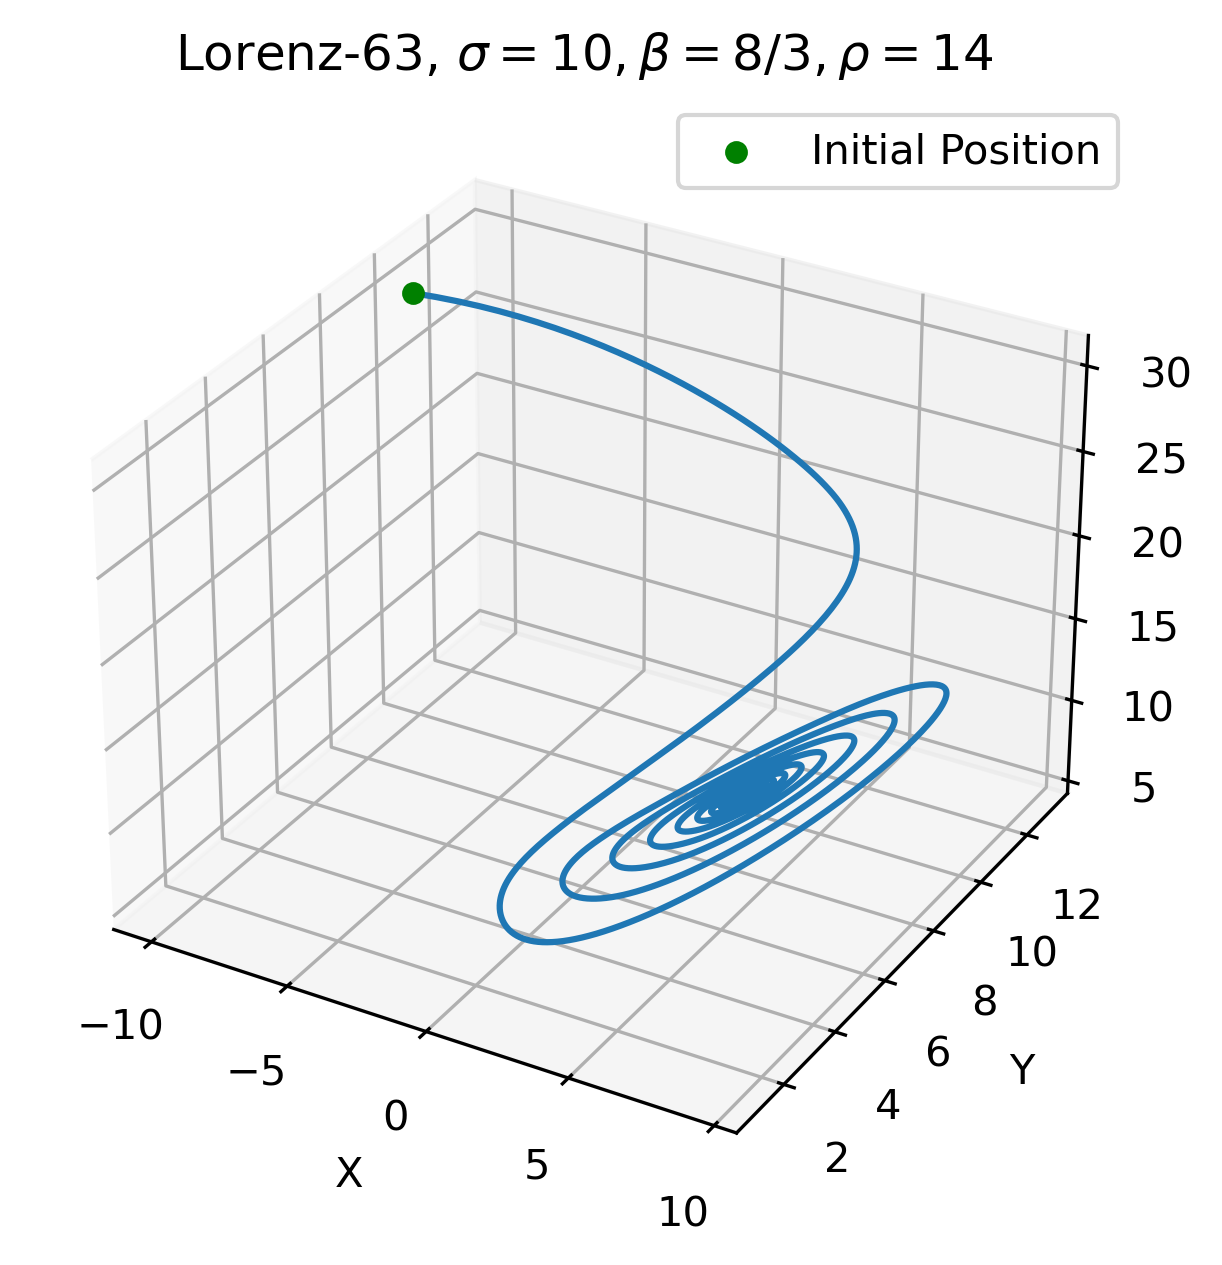
\includegraphics[scale=0.8]{graphics/Lorenz63_14.png}
    \caption{\textit{The evolution of the Lorenz-63 Model when $\sigma=10, \beta=8/3, \rho=14$ where the initial position is $\textbf{X} = (-10,10,30)^T$.}}
    \label{fig:lor63r14}
\end{figure}
\begin{figure}
    \centering
    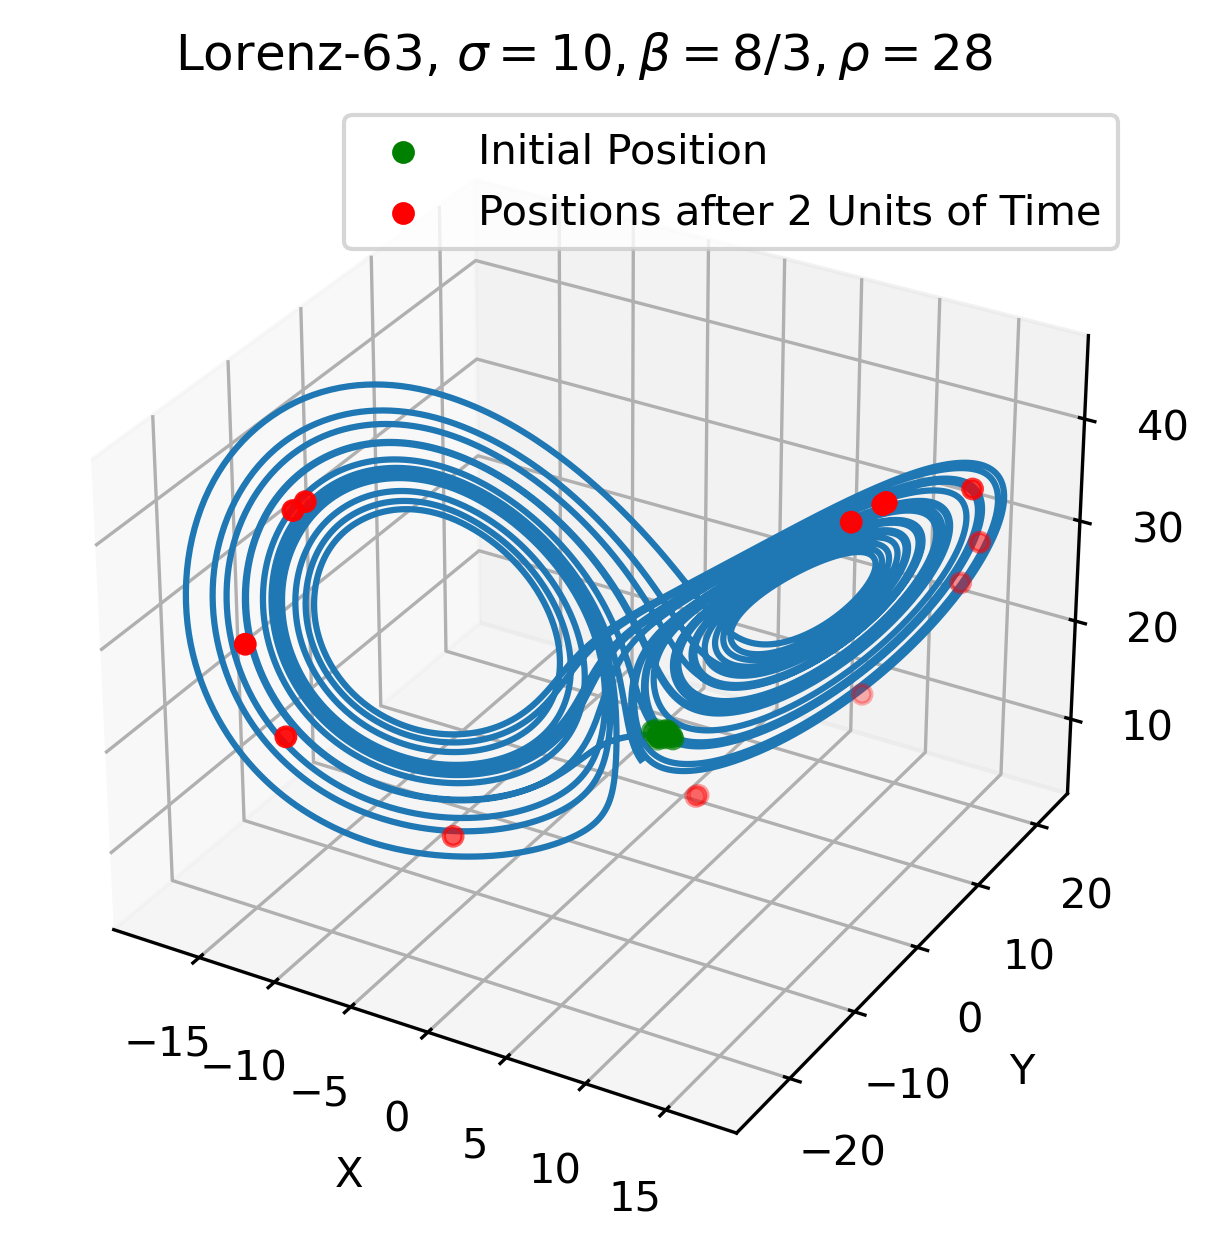
\includegraphics[scale=0.8]{graphics/Lorenz63_28.png}
    \caption{\textit{The evolution of the Lorenz-63 Model when $\sigma=10, \beta=8/3, \rho=28$ where the initial position is $\textbf{X} = (5,-5,20)^T$. An extra of 15 particles (overlapping green dots) are generated nearby and their positions after integration over 2 units of time are shown as red dots.}}
    \label{fig:lor63r28}
\end{figure}

\section{Python Programming}

In this section, we will show the necessary codes to produce Figures \ref{fig:lor63r14} and \ref{fig:lor63r28}. First, we need to use the \verb|solve_ivp| function from \verb|scipy.integrate| to integrate the dynamical system. We will define the equations of the Lorenz-63 Model as a function of $t$ and $\textbf{X}$ (which is denoted by the variable \verb|y| in the argument).
\begin{lstlisting}
import matplotlib.pyplot as plt
import numpy as np
from scipy.integrate import solve_ivp

def Lorenz63(t, y, sigma=10, beta=8/3, rho=14):
    X, Y, Z = y[0], y[1], y[2]
    dXdt = -sigma*X + sigma*Y
    dYdt = -X*Z + rho*X - Y
    dZdt = X*Y - beta*Z
    return([dXdt, dYdt, dZdt])
\end{lstlisting}
Then we will set the period of integration and the initial position of the particle.
\begin{lstlisting}
t_span = [0,25]
Y_0 = [-10,10,30]
\end{lstlisting}
Finally, we simply provide the defined \verb|Lorenz63| function for \verb|solve_ivp| to integrate.
\begin{lstlisting}
sol = solve_ivp(Lorenz63, t_span, Y_0, t_eval=np.linspace(t_span[0], t_span[1], 10000))
\end{lstlisting}
where \verb|t_eval| controls the frequency of sampling ($10000$ evenly spaced time steps here). To plot the results, we need to use the 3D projection and extract \verb|sol.y|:
\begin{lstlisting}
fig = plt.figure()
ax = plt.subplot(projection='3d')
ax.set_title("Lorenz-63, " r"$\sigma=10, \beta=8/3, \rho=14$")
ax.set_xlabel("X")
ax.set_ylabel("Y")
ax.set_zlabel("Z")
ax.scatter(*Y_0, c="g", label="Initial Position")
ax.plot(*sol.y)
ax.legend()
fig.savefig("Lorenz63_14", dpi=300, bbox_inches="tight")    
\end{lstlisting}
To run this with different parameters, we can give \verb|args| in \verb|solve_ivp|. Now we set $\rho = 28$ to enable chaotic behavior. The asterisk \verb|*| effectively expands the arrays into the three-directional components.
\begin{lstlisting}
Y_0 = [5,-5,20]
sol = solve_ivp(Lorenz63, t_span, Y_0, t_eval=np.linspace(t_span[0], t_span[1], 10000), args=(10,8/3,28))

# Other plotting commands are the same and hence omitted.
ax.scatter(*Y_0, c="g", label="Initial Position")
ax.plot(*sol.y)
\end{lstlisting}
We will add some perturbations to the initial position of the particle via Gaussian noises. 15 new particles are generated in this way.
\begin{lstlisting}
n = 15
noises = np.random.multivariate_normal([0,0,0], np.diag([0.1]*3), n)
Ys_perturb = noises + Y_0    
\end{lstlisting}
We repeat the integration procedure for all particles. Their positions after 2 units of time are then plotted as well.
\begin{lstlisting}
Ys_t2 = np.full(Ys_perturb.shape, np.nan)
for ii in np.arange(n):
    sol_p = solve_ivp(Lorenz63, [0,2], Ys_perturb[ii,:], args=(10,8/3,28))
    Ys_t2[ii,:] = sol_p.y[:,-1]
    
# Other plotting commands are the same and hence omitted.
#ax.scatter(*Ys_perturb.T, c="g")
ax.scatter(*Ys_t2.T, c="r", label="Positions after 2 Units of Time")
fig.savefig("Lorenz63_28", dpi=300, bbox_inches="tight")
\end{lstlisting}

\section{Exercises}

\begin{Exercise}
Determine the type of equilibrium point at the origin for the two-dimensional linear dynamical system $\textbf{y}' = A\textbf{y}$ where $A =$
\begin{enumerate}[label=(\alph*)]
    \item $\left[\begin{array}{@{\,}wc{12pt}wc{12pt}@{\,}}
    -1&-1\\ 
    0&-2
    \end{array}\right]$;
    \item $\left[\begin{array}{@{\,}wc{12pt}wc{12pt}@{\,}}
    0&-1\\ 
    2&2
    \end{array}\right]$;
    \item $\left[\begin{array}{@{\,}wc{12pt}wc{12pt}@{\,}}
    3&-2\\ 
    1&0
    \end{array}\right]$;
    \item $\left[\begin{array}{@{\,}wc{12pt}wc{12pt}@{\,}}
    1&-1\\ 
    -2&2
    \end{array}\right]$
\end{enumerate}
and find their general solution.
\end{Exercise}

\begin{Exercise}
Describe the equilibrium point for the three-dimensional linear dynamical system $\textbf{y}' = A\textbf{y} + \textbf{G}$ where
\begin{align*}
A &= 
\begin{bmatrix}
-1&3&-1\\ 
1&1&-3\\ 
-2&2&-2
\end{bmatrix}
& & G=
\begin{bmatrix}
1 \\
-3 \\
2
\end{bmatrix}
\end{align*}
\end{Exercise}

\begin{Exercise}
Find all equilibrium points for the following two-dimensional non-linear dynamical system
\begin{empheq}[left={\empheqlbrace}]{alignat=1}
\frac{dx}{dt} &= x^2 - y^2 + xy \nonumber \\ 
\frac{dy}{dt} &= x^2 + y^2 - 1 \nonumber
\end{empheq}
and discuss their stability.
\end{Exercise}

\begin{Exercise}
Examine the chaotic behavior of the \textit{Rössler attractor}:
\begin{subequations}
\begin{empheq}[left={\empheqlbrace}]{alignat=1}
\frac{dx}{dt} &= -y-z \\ 
\frac{dy}{dt} &= x+ay \\
\frac{dz}{dt} &= b+z(x-c)
\end{empheq}
\end{subequations}
with three parameters $a=0.2, b=0.2, c=5.7$ and plot it.
\end{Exercise}
\chapter{Index Notation and Introduction to Tensors}
\label{chapter:Tensor}

This is the final chapter of this book. (Congratulations!) It will be revealed that, matrices (or to be accurate, linear transformations), along with vectors, actually can be generalized to a broader class of objects known as \textit{tensors}. In the simplest sense, tensors are quantities with subscripts. To facilitate the manipulation of these subscripts, we will introduce the handy \textit{Index Notation}, as well as the \textit{Kronecker delta/epsilon symbols}. The next step is to develop \textit{matrix/tensor calculus} where several important differentiation rules and integral theorems will be given. Tensors can have physical meanings, allowing us to apply them in many scenarios. One of their usages in Earth Science is to serve as the language in \textit{Continuum Mechanics}. On the other hand, the related matrix calculus is much needed in \textit{Data Assimilation}, which is a technique in Atmospheric Sciences to rectify the output of a forecast from a weather model with available observations.

\section{Index Notation and Tensors}

\subsection{Rules of Index Notation}

Previously, we have usually been writing matrix multiplications along the lines of $AB = C$ or $A\vec{x} = \smash{\vec{h}}$ without explicitly showing the subscripts and summation symbol. However, if we choose to do so, then they can be expressed as
\begin{align*}
\sum_{k=1}^r A_{ik}B_{kj} &= C_{ij} &  & \sum_{j=1}^n A_{ij}x_j = h_i
\end{align*}
However, the summation symbol is clumsy to be included every time, especially when it involves a chain of products like $ABCD$. The \index{Index Notation}\keywordhl{Index Notation} (also known as the \index{Einstein Convention}\keywordhl{Einstein Convention}) solves this problem by assuming that any subscript appearing exactly twice in an additive term will be summed (\textit{contracted}) implicitly over all values that the subscript can take. This also means that any such pair of repeated subscripts must
occur only in positions with the same range of values. Consequentially, the above examples are simplified into
\begin{align*}
A_{ik}B_{kj} &= C_{ij} &  & A_{ij}x_j = h_i    
\end{align*}
To be more clear, subscripts that appear exactly twice in any additive term are called \index{Summation Indices}\keywordhl{summation indices} (or \index{Dummy Indices}\keywordhl{dummy indices}) and are summed over specific values which are often automatically inferred from the situation (for example, in three-dimensional physical problems, they will usually take the explicit values of $1,2,3$.). On the other hand, subscripts that only appear once in \textit{every} additive term of an expression or equation are known as \index{Free Indices}\keywordhl{free indices}. In the first example above, $k$ is the dummy index, while $i, j$ are free indices. (How about the second example?\footnote{$j$ is the dummy index and $i$ is the free index.}) There are some other important points about the Index Notation to be emphasized: First, it is not allowed for a subscript to appear more than twice within a single additive term (so we cannot write $A_{ik}B_{kj}C_{kl}$, although it is okay for a dummy subscript to appear twice in multiple additive terms, e.g. $A_{ik}B_{kj} + C_{ij}D_{kk}$); Second, any pair of dummy indices can be replaced by any other alphabets (e.g. $A_{ik}B_{kj}$ is equivalent to $A_{il}B_{lj}$) but the free indices cannot be changed arbitrarily; Finally, as just mentioned, all free indices have to appear once and only once in every additive term (on both sides if it is an equation) (so $A_i + B_{ij}C_{j} + D_{ikk}$ is acceptable but not $A_{ij} + B_{kkj}$). As long as the quantities have their subscripts written out, the order of the quantities (but not their indices) is unimportant. Below we give some examples of the Index Notation in a three-dimensional setting:
\begin{enumerate}
    \item $a_ib_i = \sum_{i=1}^3 a_ib_i = a_1b_1 + a_2b_2 + a_3b_3$
    \item $A_{kk} = \sum_{k=1}^3 A_{kk} = A_{11} + A_{22} + A_{33}$
    \item $A_{ik}B_{jk} = \sum_{k=1}^3 A_{ik}B_{jk} = A_{i1}B_{j1} + A_{i2}B_{j2} + A_{i3}B_{j3}$
    \item \begin{align*}
    A_{ijk}B_{jl}C_{km} &= \sum_{j=1}^3 \sum_{k=1}^3 A_{ijk}B_{jl}C_{km} \\
    &= A_{i11}B_{1l}C_{1m} + A_{i12}B_{1l}C_{2m} + A_{i13}B_{1l}C_{3m} \\
    &\quad + A_{i21}B_{2l}C_{1m} + A_{i22}B_{2l}C_{2m} + A_{i23}B_{2l}C_{3m} \\
    &\quad + A_{i31}B_{3l}C_{1m} + A_{i32}B_{3l}C_{2m} + A_{i33}B_{3l}C_{3m} \\
    &\coloneq Y_{ilm}
    \end{align*}
    will be a subscripted quantity with 3 free indices $i, l, m$ where each additive term contains $3^2 = 9$ smaller terms.
    \item \begin{align*}
    A_{ikl}B_{jkm}C_{lm} &= \sum_{k=1}^3 \sum_{l=1}^3 \sum_{m=1}^3 A_{ikl}B_{jkm}C_{lm} \\
    &\coloneq Z_{ij}
    \end{align*}
    will be a subscripted quantity with 2 free indices $i, j$ where each additive term contains $3^3 = 27$ smaller terms.
    \item $A_{ij}B_{ijkl}C_{kl} = \smash{\sum_{i=1}^3 \sum_{j=1}^3 \sum_{k=1}^3 \sum_{l=1}^3} A_{ij}B_{ijkl}C_{kl} \coloneq X$ will be a scalar quantity without free indices consisting of $3^4 = 81$ smaller terms.
\end{enumerate}
Short Exercise: Determine whether the following equations are valid or not, and justify your answers.\footnote{Incorrect ($j$ appears three times in the single additive term on R.H.S.), Correct ($i,j$ are free indices and $k,l$ are dummy indices), Incorrect ($j$ appears twice on L.H.S. but once on R.H.S), Correct (All subscripts are dummy indices and all additive terms are scalars), Incorrect ($i,j$ cannot be free and dummy indices at the same time).}
\begin{enumerate}
    \item $x_i = u_jv_{ijj}$;
    \item $A_{ij} = B_{ik}C_{kj} + D_{jl}x_iy_l$;
    \item $A_{ij}x_j = B_{ij}$;
    \item $A_{ii} + u_jv_j = B_{kl}C_{km}w_{lm} - 1$;
    \item $A_{ij} + B_{ij}C_{ij} = D_{ij}$.
\end{enumerate}

\subsection{Kronecker Delta and Epsilon Symbols}

Before getting to know about the \textit{Kronecker delta/epsilon symbols}, it is helpful to denote the three-dimensional Cartesian standard unit vectors $\hat{\imath} = \hat{e}^{(1)}$, $\hat{\jmath} = \hat{e}^{(2)}$, $\hat{k} = \hat{e}^{(3)}$ by $\textbf{e}_1, \textbf{e}_2, \textbf{e}_3$ to switch and ensure the consistency of notation. We will assume that the problem is always three-dimensional so that every index always runs through $1,2,3$ unless otherwise specified. Therefore, given any three-dimensional vector $\textbf{u} = (u_1, u_2, u_3)^T$, it can be expressed by 
\begin{align}
\textbf{u} = u_1 \textbf{e}_1 + u_2 \textbf{e}_2 + u_3 \textbf{e}_3 = u_i \textbf{e}_i
\end{align}
using the Index Notation. Now, the \index{Kronecker Delta}\keywordhl{Kronecker delta} symbol is defined as
\begin{defn}[Kronecker Delta Symbol]
The Kronecker delta symbol is a quantity with $2$ subscripts such that
\begin{align}
\delta_{ij} = \begin{cases}
1 & \text{if $i=j$} \\
0 & \text{if $i\neq j$}
\end{cases}    
\label{eqn:krondef}
\end{align}
\end{defn}
Compared with Definition \ref{defn:identity}, it works like and can be treated as an identity matrix, although there are some subtle differences between them. Due to the definition of the delta symbol, its effect is to replace a dummy index with the other index. For example,
\begin{align*}
A_{ij}\delta_{jk} &= A_{ik} & & A_{ij}B_{kl}\delta_{jl} = A_{ij}B_{kj}
\end{align*}
since only when $j = k$ the delta symbol will be equal to $1$ and otherwise $0$ in the first case (how about the second case?). Recall that for the standard unit vectors, we have
\begin{subequations}
\begin{align}
\textbf{e}_1 \cdot \textbf{e}_1 = \textbf{e}_2 \cdot \textbf{e}_2 = \textbf{e}_3 \cdot \textbf{e}_3 &= 1 \\
\textbf{e}_1 \cdot \textbf{e}_2 = \textbf{e}_1 \cdot \textbf{e}_3 = \textbf{e}_2 \cdot \textbf{e}_3 &= 0
\end{align}
\end{subequations}
or more succinctly,
\begin{align}
\textbf{e}_i \cdot \textbf{e}_j = \begin{cases}
1 & \text{if $i=j$} \\
0 & \text{if $i\neq j$}
\end{cases}    
\end{align}
Hence we can define the Kronecker delta symbol via
\begin{align}
\delta_{ij} = \textbf{e}_i \cdot \textbf{e}_j \label{eqn:kronee}
\end{align}
With this, we can derive (\ref{eqn:dotreal}) in Definition \ref{defn:dotreal} for the real dot product in a new way:
\begin{align}
\textbf{u} \cdot \textbf{v} &= (u_i \textbf{e}_i) \cdot (v_j \textbf{e}_j) \nonumber \\
&= u_iv_j (\textbf{e}_i \cdot \textbf{e}_j) \nonumber \\
&= u_iv_j \delta_{ij} & \text{(by (\ref{eqn:kronee}))} \nonumber \\
&= u_iv_i \label{eqn:dotind}
\end{align}
On the other hand, the \index{Epsilon Symbol}\index{Permutation Symbol}\keywordhl{epsilon (permutation)} symbol (or the \index{Levi-Civita Symbol}\keywordhl{Levi-Civita symbol}) is defined as
\begin{defn}[Levi-Civita Epsilon Symbol]
\label{defn:epsilon}
The epsilon permutation symbol is a quantity with $3$ subscripts such that
\begin{align}
\label{eqn:epsilon}
\epsilon_{ijk} =
\begin{cases}
0 & \text{if any two indices are equal} \\
+1 & \begin{aligned}
&\text{if $(i,j,k)$ is an even permutation of $(1,2,3)$,} \\
&\text{i.e.\ $(1,2,3), (2,3,1), (3,1,2)$}
\end{aligned}  \\
-1 & \begin{aligned}
&\text{if $(i,j,k)$ is an odd permutation of $(1,2,3)$,} \\
&\text{i.e.\ $(2,1,3), (3,2,1), (1,3,2)$}
\end{aligned}
\end{cases}    
\end{align}
\end{defn}
Similarly, recall that from Definition \ref{defn:crossijk}, we have
\begin{subequations}
\begin{align}
\textbf{e}_1 \times \textbf{e}_2 &= \textbf{e}_3, \textbf{e}_2 \times \textbf{e}_1 = -\textbf{e}_3 \\
\textbf{e}_2 \times \textbf{e}_3 &= \textbf{e}_1, \textbf{e}_3 \times \textbf{e}_2 = -\textbf{e}_1 \\
\textbf{e}_3 \times \textbf{e}_1 &= \textbf{e}_2, \textbf{e}_1 \times \textbf{e}_3 = -\textbf{e}_2 \\
\textbf{e}_1 \times \textbf{e}_1 &= \textbf{e}_2 \times \textbf{e}_2 = \textbf{e}_3 \times \textbf{e}_3 = \textbf{0}
\end{align}   
\end{subequations}
and thus by going through all the cases, they can be summarized as
\begin{align}
\textbf{e}_i \times \textbf{e}_j= \epsilon_{ijk} \textbf{e}_k \label{eqn:epsilonee}
\end{align}
By taking a dot product with $\textbf{e}_l$ on both sides and adjusting the indices, we can arrive at an equivalent definition of the epsilon symbol:
\begin{align}
\textbf{e}_l \cdot (\textbf{e}_i \times \textbf{e}_j) &= \epsilon_{ijk} (\textbf{e}_l \cdot \textbf{e}_k)  \nonumber \\
\textbf{e}_l \cdot (\textbf{e}_i \times \textbf{e}_j) &= \epsilon_{ijk} \delta_{lk} \nonumber \\
\textbf{e}_l \cdot (\textbf{e}_i \times \textbf{e}_j) &= \epsilon_{ijl} \nonumber \\
\textbf{e}_k \cdot (\textbf{e}_i \times \textbf{e}_j) &= \epsilon_{ijk} \nonumber & \begin{aligned}
&\text{(Replacing a free index $l \to k$} \\
&\text{on both sides simultaneously is allowed)}     
\end{aligned} \\
\epsilon_{jki} &= \textbf{e}_i \cdot (\textbf{e}_j \times \textbf{e}_k) & \text{(Rotating the free indices $k \to i$, $i \to j$, $j \to k$)}  \nonumber \\
\epsilon_{ijk} &= \textbf{e}_i \cdot (\textbf{e}_j \times \textbf{e}_k) 
&\begin{aligned}
&\text{($(j,k,i)$ is an even permutation of $(i,j,k)$} \\
&\text{and can be rotated within the epsilon symbol)}    
\end{aligned} 
\end{align}
In the same spirit, we can derive the formula of cross product in Properties \ref{proper:crossdet} by the Index Notation as follows.
\begin{align}
\textbf{u} \times \textbf{v} &= u_i\textbf{e}_i \times v_j\textbf{e}_j \nonumber \\
&= u_iv_j (\textbf{e}_i \times \textbf{e}_j) \nonumber \\
&= u_iv_j \epsilon_{ijk} \textbf{e}_k \label{eqn:crossind} \\
& \text{(by (\ref{eqn:epsilonee}))} \nonumber \\
&= (u_2v_3 - u_3v_2)\textbf{e}_1 + (u_3v_1 - u_1v_3)\textbf{e}_2 + (u_1v_2 - u_2v_1)\textbf{e}_3 \nonumber \\
& \text{(Direct expansion using (\ref{eqn:epsilon}) in Definition \ref{defn:epsilon})} \nonumber
\end{align}
Comparing with the determinant form of cross product (\ref{eqn:crossdet}) in Properties \ref{proper:crossdet}, we have
\begin{align}
\textbf{u} \times \textbf{v} = u_iv_j \epsilon_{ijk} \textbf{e}_k = 
\begin{vmatrix}
\textbf{e}_1 & \textbf{e}_2 & \textbf{e}_3 \\
u_1 & u_2 & u_3 \\
v_1 & v_2 & v_3
\end{vmatrix}
\label{eqn:crosstens}
\end{align}
Replacing $\textbf{e}_k$ by an arbitrary vector $w_k$, we arrive at an alternative formula for determinant using the Index Notation in three-dimensional vector spaces:
\begin{align}
u_iv_j \epsilon_{ijk} w_k &= 
\begin{vmatrix}
w_1 & w_2 & w_3 \\
u_1 & u_2 & u_3 \\
v_1 & v_2 & v_3
\end{vmatrix}  \nonumber \\
\epsilon_{ijk}  u_iv_jw_k &= 
\begin{vmatrix}
u_1 & u_2 & u_3 \\
v_1 & v_2 & v_3 \\
w_1 & w_2 & w_3
\end{vmatrix} \label{eqn:determinanteps1} \\
& \text{(Swapping rows twice leaves the sign of determinant unchanged)} \nonumber
\end{align}
These two symbols are closely related by the \index{Epsilon-delta Identity}\keywordhl{Epsilon-delta Identity}.
\begin{proper}[$\epsilon$--$\delta$ Identity] 
\label{proper:epsdel} Contracting over the pair of first subscripts between two epsilon symbols gives 
\begin{align}
\epsilon_{ijk}\epsilon_{imn} = \delta_{jm}\delta_{kn} - \delta_{jn}\delta_{km} \label{eqn:epsdel}
\end{align}
\end{proper}
\begin{proof}
We will use a brute-force approach and enumerate all the outcomes. Note that the R.H.S. will have values 
\begin{align}
\begin{cases}
+1 & \text{if $j=m$, $k=n$, $j\neq n$ (and thus $k\neq m$)} \\
-1 & \text{if $j=n$, $k=m$, $j\neq m$ (and thus $k\neq n$)} \\
0 & \text{Otherwise}
\end{cases}
\label{eqn:epsdel2}
\end{align}
Now consider the L.H.S. As the first indices of the two epsilons are equal and every index can only take the three values of $1,2,3$, for their product to give a non-zero value, the only two possibilities are (1) $j = m \neq i$, $k = n \neq i$, $j \neq n$; and (2) $j = n \neq i$, $k = m \neq i$, $j \neq m$ where the four free indices $j,k,m,n$ cannot take the same value as the dummy index $i$, and $j,k$ (also $m,n$) cannot be equal simultaneously. These are consistent with the first and second situations in (\ref{eqn:epsdel2}). Now we only need to justify if they really lead to the outputs of $+1$ and $-1$ respectively. In the first case, it is not hard to see that $\epsilon_{ijk}$ and $\epsilon_{imn}$ must be $+1$ or $-1$ at the same time so their product indeed gives $+1$. Similarly, in the second case, one of the epsilon symbols will be $+1$ and the other will be $-1$ ($\epsilon_{ijk} = -\epsilon_{ikj} = -\epsilon_{imn}$) so it will produce $-1$. The identity is hence established.
\end{proof}
Note that contracting one more index (e.g. $j=m$) in the identity gives
\begin{align}
\epsilon_{ijk}\epsilon_{ijn} &= \delta_{jj}\delta_{kn} - \delta_{jn}\delta_{kj} \nonumber \\
&= 3\delta_{kn} - \delta_{kn} = 2\delta_{kn}
\end{align}
as $\delta_{jj} = \delta_{11} + \delta_{22} + \delta_{33} = 1+1+1 = 3$ and in the second term the dummy index $j$ is replaced by $k$. Going one step further, contracting all three indices simply gives
\begin{align}
\epsilon_{ijk}\epsilon_{ijk} &= 2\delta_{kk} = 2(3) = 6
\end{align}
Now let's see how this identity can be used in showing other vector identities.
\begin{exmp}
Prove Formula (\ref{eqn:triplecross}) for vector triple product in Properties \ref{proper:triplecross} using the Index Notation and Epsilon-delta Identity.
\end{exmp}
\begin{solution}
Applying (\ref{eqn:crossind}) twice, we have
\begin{align*}
\vec{u} \times (\vec{v} \times \vec{w}) &= (u_j\textbf{e}_j) \times (v_mw_n\epsilon_{mni}\textbf{e}_i) \\
&= (u_j\epsilon_{jik}(v_mw_n\epsilon_{mni})) \textbf{e}_k \\
&= \epsilon_{ikj}\epsilon_{imn}u_jv_mw_n \textbf{e}_k \\
&= (\delta_{km}\delta_{jn} - \delta_{kn}\delta_{jm})(u_jv_mw_n \textbf{e}_k) & \text{((\ref{eqn:epsdel}) in Properties \ref{proper:epsdel})} \\
&= u_jv_kw_j \textbf{e}_k - u_jv_jw_k \textbf{e}_k \\
&= (u_jw_j)(v_k\textbf{e}_k) - (u_jv_j)(w_k \textbf{e}_k) \\
&= (\vec{u} \cdot \vec{w})\vec{v} - (\vec{u} \cdot \vec{v})\vec{w} & \text{(by (\ref{eqn:dotind}))}
\end{align*}
\end{solution}
When there is no ambiguity, we will omit the standard unit vector symbol $\textbf{e}_k$ so that, for example, the second-to-last line above is simply $(u_jw_j)v_k - (u_jv_j)w_k$ and a vector $\vec{v}$ is simply denoted by something like $v_i$.

\subsection{Transformation and Quotient Laws for Tensors}

Now we will formally introduce \index{Tensors}\keywordhl{tensors}. A scalar is a rank-$0$ tensor and a vector is a rank-$1$ tensor. The \index{Rank (of a Tensor)}\keywordhl{rank} of a tensor (not to be confused with the rank of a matrix) is the number of its subscripts. Linear transformations or bilinear forms will be rank-$2$ tensors where the associated matrices serve as their representations in certain coordinate systems. Note that this explanation is a largely simplified one and for Mathematicians the definition will be much more rigorous.\footnote{\label{foot:rstensor}Going into depth, the rank of a tensor is actually given by a $2$-tuple $(r,s)$ which means that it receives $r$ \textit{covectors} and $s$ vectors to output a scalar. A covector takes one vector to produce a scalar and hence by definition is a $(0,1)$-tensor, while vice versa a vector will take one covector to also produce a scalar and is a $(1,0)$-tensor. Linear transformations are usually treated as $(1,1)$-tensors while bilinear forms are $(0,2)$-tensors. $r$ and $s$ indicates the number of \textit{contravariant}/\textit{covariant} indices.} But for Physicists or Earth Scientists, it is adequate to know that a rank-$r$ tensor \textit{"transforms like a tensor"}, obeying the so-called \textit{Transformation Law}. To this end, we first need to revisit how a coordinate transformation is carried out. As in (\ref{eqn:PBB'}), the change of coordinates matrix is
\begin{align}
P_\beta^{\beta'} = \begin{bmatrix}
[\vec{v}_\beta^{(1)}]_{\beta'} | [\vec{v}_\beta^{(2)}]_{\beta'} | \cdots | [\vec{v}_\beta^{(n)}]_{\beta'}
\end{bmatrix}
\end{align}
In most of Earth Science usages, the coordinate systems used will be orthonormal and we will assume this is so for the rest of the chapter. This makes the tensors \textit{Cartesian}. By Properties \ref{proper:orthocoords}, the coordinates of any vector in the new orthonormal coordinate system relative to the old orthonormal coordinate system can be found by direct projection and vice versa. Therefore, if we denote the old and new orthonormal basis by $\beta = \{\textbf{e}_1, \textbf{e}_2, \textbf{e}_3\}$ and $\beta'= \{\textbf{e}'_1, \textbf{e}'_2, \textbf{e}'_3\}$, the change of coordinates matrix will become
\begin{align}
P_\beta^{\beta'} = \begin{bmatrix}
\textbf{e}_1 \cdot \textbf{e}'_1 & \textbf{e}_2 \cdot \textbf{e}'_1 & \textbf{e}_3 \cdot \textbf{e}'_1 \\
\textbf{e}_1 \cdot \textbf{e}'_2 & \textbf{e}_2 \cdot \textbf{e}'_2 & \textbf{e}_3 \cdot \textbf{e}'_2 \\
\textbf{e}_1 \cdot \textbf{e}'_3 & \textbf{e}_2 \cdot \textbf{e}'_3 & \textbf{e}_3 \cdot \textbf{e}'_3 
\end{bmatrix}
= \textbf{e}_j \cdot \textbf{e}'_i
\label{eqn:Peeij}
\end{align}
This is an orthogonal matrix\footnote{\label{foot:orthodelta} Extending Properties \ref{proper:orthocoords}, we have $\textbf{e}'_{j} = (\textbf{e}'_{j} \cdot \textbf{e}_{k})\textbf{e}_{k}$ which expresses any new basis vector in terms of the sum of projections onto the old orthonormal basis. By considering $\textbf{e}'_{i} \cdot \textbf{e}'_{j} = \delta_{ij}$ due to (\ref{eqn:kronee}) (valid for any orthonormal basis), we have
\vspace{\maxdimen}
\begin{align*}
(\textbf{e}'_{i} \cdot \textbf{e}_{k})\textbf{e}_{k} \cdot (\textbf{e}'_{j} \cdot \textbf{e}_{l})\textbf{e}_{l} &= \delta_{ij} \\
(\textbf{e}'_{i} \cdot \textbf{e}_{k})(\textbf{e}'_{j} \cdot \textbf{e}_{l})(\textbf{e}_{k} \cdot \textbf{e}_{l}) &= \delta_{ij} \\
(\textbf{e}'_{i} \cdot \textbf{e}_{k})(\textbf{e}'_{j} \cdot \textbf{e}_{l})\delta_{kl} &= \delta_{ij} & \text{($\textbf{e}_{k} \cdot \textbf{e}_{l} = \delta_{kl}$ from (\ref{eqn:kronee}) as well)} \\
(\textbf{e}'_{i} \cdot \textbf{e}_{k})(\textbf{e}'_{j} \cdot \textbf{e}_{k}) &= \delta_{ij}
\end{align*} where the L.H.S. is essentially $(\textbf{e}'_{i} \cdot \textbf{e}_{k})(\textbf{e}_{k} \cdot \textbf{e}'_{j}) = [\smash{(P_\beta^{\beta'})^T}]_{ik}[\smash{P_\beta^{\beta'}}]_{kj}$ and R.H.S. is effectively an identity matrix, so by Properties \ref{proper:orthoinvT} we are done.}, and by (\ref{eqn:bijectvTv}), any vector $\vec{v}$ (that is also a rank-$1$ tensor) is transformed according to
\begin{align}
[\vec{v}]' &= P_\beta^{\beta'}[\vec{v}] \nonumber \\
v'_i &= (\textbf{e}_j \cdot \textbf{e}'_i) v_j \nonumber \\
v'_j &= (\textbf{e}_i \cdot \textbf{e}'_j) v_i 
\end{align}
where we only keep the prime to denote the new coordinate frame as a shorthand and have swapped the indices in the last line. From now on, we will write 
\begin{align}
a_{ij} = \textbf{e}_i \cdot \textbf{e}'_j \label{eqn:aij}
\end{align} for convenience, so the above becomes $v'_j = a_{ij}v_i$. Similarly, for a rank-$2$ tensor $F$, be it a linear transformation or bilinear form, it is transformed as
\begin{align}
F'_{kl} = a_{ik} a_{jl} F_{ij} \label{eqn:rank2aF}
\end{align}
This is consistent with both Properties \ref{proper:endomorph} and Definition \ref{defn:coordtransquad} at the same time, because the change of coordinates matrix is orthogonal and so $[a^{-1}]_{ki} = [a^T]_{ki} = a_{ik}$ by Properties \ref{proper:orthoinvT}. In general, the \keywordhl{Transformation Law} says
\begin{proper}
\label{proper:translaw}
A rank-$r$ \textit{Cartesian} tensor $T$ is a quantity that transforms according to the rule\footnotemark
\begin{align}
T'_{ijkl\ldots} = a_{mi}a_{nj}a_{pk}a_{ql}\cdots T_{mnpq\ldots}
\end{align}
where $a_{**}$ invokes the orthogonal transformation matrix as in (\ref{eqn:aij}).
\end{proper}
\footnotetext{As we are sticking with orthonormal coordinate systems and orthogonal transformations only, the difference between contravariant/covariant indices (as mentioned in Footnote \ref{foot:rstensor}) and hence superscripts/subscripts can be safely ignored for Cartesian tensors. If you don't understand any of what I am saying, ignore this footnote as well.} Physically, it means that tensors are coordinate-independent quantities even though they can have different coordinate representations: These different representations have to be consistent and abide by the Transformation Law so that they still reflect the same physical quantity no matter the choice of coordinate system. Moreover, it implies that to consider if a quantity is a tensor requires a physical context as hinted by the example below.
\begin{exmp}
Show that the following quantities $T = (v_1, v_2) = $ 
\begin{enumerate}[label=(\alph*)]
    \item $(x_2,x_1)$
    \item $(x_1^2,x_1x_2)$
\end{enumerate}
are actually not rank-$1$ Cartesian tensors despite looking like vectors (where the index only takes the values of $1,2$ here).
\end{exmp}
\begin{solution}
For (a), the usual coordinate transformations on $x$ and $y$ respectively by an orthogonal rotation over the plane of a degree $\theta$ are given by (\ref{eqn:2drotate}):
\begin{empheq}[left={\empheqlbrace}]{alignat=1}
x_1' &= (\cos \theta) x_1 + (\sin\theta) x_2 = v_2' \nonumber\\
x_2' &= (-\sin \theta) x_1 + (\cos\theta) x_2 = v_1' \nonumber
\end{empheq}
However, the Transformation Law (Properties \ref{proper:translaw}) requires that
\begin{align*}
v_1' = T'_1 &= a_{11}T_1 + a_{21}T_2 \\
&= (\cos \theta) x_2 + (\sin \theta) x_1 \\
v_2' = T'_2 &= a_{12}T_1 + a_{22}T_2 \\
&= (-\sin\theta) x_2 + (\cos\theta) x_1
\end{align*}
where 
\begin{align*}
a_{ij} &= \textbf{e}_i \cdot \textbf{e}'_j \\
\begin{bmatrix}
a_{11} & a_{12} \\
a_{21} & a_{22}
\end{bmatrix}
&= 
\left[\begin{array}{@{\,}wc{25pt}wc{30pt}@{\,}}
\textbf{e}_1 \cdot \textbf{e}'_1 & \textbf{e}_1 \cdot \textbf{e}'_2 \\
\textbf{e}_2 \cdot \textbf{e}'_1 & \textbf{e}_2 \cdot \textbf{e}'_2
\end{array}\right]
\\
&=
\left[\begin{array}{@{\,}wc{25pt}wc{30pt}@{\,}}
\cos\theta & -\sin\theta \\
\sin\theta & \cos\theta
\end{array}\right]
\end{align*}
These two do not match. For (b), we similarly have
\begin{align*}
v_1' = (x_1')^2 &= ((\cos \theta) x_1 + (\sin\theta) x_2)^2 \\
&= (\cos \theta)^2 x_1^2 + (\cos \theta)(\sin\theta) x_1x_2 + (\sin\theta)^2 x_2^2
\end{align*}
for the first component, but the Transformation Law demands that
\begin{align*}
v_1' = T'_1 = (x_1^2)' &= a_{11}T_1 + a_{21}T_2 \\
&= (\cos \theta) x_1^2 + (\sin \theta) x_1x_2
\end{align*}
They are clearly incompatible. Nevertheless, it is quite easy to see that the intuitive displacement vector $\vec{x} = (x_1,x_2)^T$, as well as $(x_2,-x_1)^T$, will be a rank-$1$ tensor (we leave the verification to the readers\footnote{For the second case $T = (x_2, -x_1)$, the usual coordinate transformation is the essentially same as in part (a) of the example but with an extra negative sign for the second component, whereas the Transformation Law works as
\begin{align*}
v_1' = T'_1 &= a_{11}T_1 + a_{21}T_2 \\
&= (\cos \theta) x_2 + (\sin \theta) (-x_1) \\
&= (\cos \theta) x_2 + (-\sin \theta) x_1 = x_2' \\
v_2' = T'_2 &= a_{12}T_1 + a_{22}T_2 \\
&= (-\sin\theta) x_2 + (\cos\theta) (-x_1) \\
&= -[(\cos \theta) x_2 + (\sin\theta) x_1] = -x_1'
\end{align*} so they are consistent.}).
\end{solution}
It is not hard to show that the product of two tensors is a tensor.\footnote{For example, if $C_{ij\ldots pq\ldots} = A_{ij\ldots}B_{pq\ldots}$ where $A$ and $B$ are tensors, then each of the smaller tensors will transform accordingly on its own: $A'_{mn\ldots} = a_{im}a_{jn}\cdots A_{ij\ldots}$, $B'_{sr\ldots} = a_{ps}a_{qr}\cdots B_{pq\ldots}$, and thus
\begin{align*}
C'_{mn\ldots sr\ldots} = A'_{mn\ldots}B'_{sr\ldots} &= a_{im}a_{jn}\cdots a_{ps}a_{qr}\cdots A_{ij\ldots} B_{pq\ldots} \\
&= a_{im}a_{jn}\cdots a_{ps}a_{qr}\cdots C_{ij\ldots pq\ldots}
\end{align*} will also transform as indicated by Properties \ref{proper:translaw}.} Therefore, kinetic energy (per unit mass) in Newtonian Mechanics $\frac{1}{2}(\vec{v} \cdot \vec{v}) = \frac{1}{2}v_iv_i$ is a rank-$0$ tensor (scalar) if we gladly accept the intuitive premise that the velocity $\vec{v} = v_i$ is a rank-$1$ tensor (vector). In addition, there is another way to quickly verify if a quantity is a tensor by the \keywordhl{Quotient Law} which works in the other way around.
\begin{thm}[Quotient Law]
\label{thm:quotientl}
If $A_{ij\ldots n}$ is a $n$-subscripted quantity, $B_{pq\ldots m}$ is known to be a rank-$m$ tensor, and the product
\begin{align*}
C_{ij\ldots npq \ldots m} = A_{ij\ldots k\ldots n} B_{pq\ldots k\ldots m}   
\end{align*}
is also a tensor of rank $n+m-2k$ where $k \geq 1$ is the amount of index contraction, then $A_{ij\ldots n}$ will be a rank-$n$ tensor.
\end{thm}
With this, we can easily show that some other commonly seen physical quantities are tensors. It will be of use later. 

\subsection{Isotropic Tensors}

Here we will revisit the Kronecker delta and epsilon symbols. In fact, they qualify as a rank-$2$ and rank-$3$ tensor respectively. Moreover, they are further \index{Isotropic}\keywordhl{isotropic} tensors in the sense that they have the same representation (i.e.\ no directionality) in any coordinate system under the Transformation Law. From another perspective, it has to be isotropic since their components are all constants ($0$, $1$, or $-1$) and the usual coordinate transformation should have no effect on them. Now we will explicitly show the isotropic attribute for the Kronecker delta first. The Transformation Law (Properties \ref{proper:translaw}) requires that
\begin{align}
\delta'_{ij} = \delta_{ij}
\end{align}
and the L.H.S. will transform as
\begin{align*}
\delta'_{ij} &= a_{ki}a_{lj}\delta_{kl} \\
&= a_{ki}a_{kj} \\
&= [a^T]_{ik}a_{kj} = \delta_{ij}
\end{align*}
since $a_{**}$ acts as an orthogonal matrix, and by Properties \ref{proper:orthoinvT}, it will equal to R.H.S. which is like an identity (also see Footnote \ref{foot:orthodelta}). This indeed shows that the Kronecker delta is a rank-$2$ isotropic tensor. In a similar vein, we want to show that
\begin{align}
\epsilon'_{ijk} = \epsilon_{ijk}
\end{align}
For this, it is beneficial to first establish that for a $3 \times 3$ matrix $L$, we can extend (\ref{eqn:determinanteps1}) as
\begin{align}
\abs{L}\epsilon_{lmn} = L_{li}L_{mj}L_{nk}\epsilon_{ijk} \label{eqn:determinanteps2}
\end{align}
where $\abs{L}$ is the determinant of $L$. This can be derived by noting that from (\ref{eqn:determinanteps1}) we have
\begin{align}
\abs{L} = L_{1i}L_{2j}L_{3k}\epsilon_{ijk} \label{eqn:determinanteps3}
\end{align}
and swapping or rotating indices, through the properties of the epsilon symbol (or equivalently those of the determinant) will give the other five non-zero possibilities
\begin{align*}
\abs{L} &= L_{2i}L_{3j}L_{1k}\epsilon_{ijk} \\
\abs{L} &= L_{3i}L_{1j}L_{2k}\epsilon_{ijk} \\
-\abs{L} &= L_{2i}L_{1j}L_{3k}\epsilon_{ijk} \\
-\abs{L} &= L_{3i}L_{2j}L_{1k}\epsilon_{ijk} \\
-\abs{L} &= L_{1i}L_{3j}L_{2k}\epsilon_{ijk}
\end{align*}
Using the epsilon symbol to combine all six cases then yields (\ref{eqn:determinanteps2}). Now the Transformation Law reads
\begin{align*}
\epsilon'_{ijk} &= a_{il}a_{jm}a_{kn}\epsilon_{lmn} \\
&= \abs{a}\epsilon_{ijk} & \text{(by (\ref{eqn:determinanteps2}))}
\end{align*}
and it equals to $\epsilon_{ijk}$ as we assume that the coordinate transformation is orthogonal and by Properties \ref{proper:orthopm1det} the determinant will take the value $\abs{a} = 1$ or $-1$. We further place the restriction that it is a \textit{proper} rotation (compared to the \textit{improper} rotation, that is, reflection) so that $\abs{a} = 1$, and hence the desired result follows. Finally, we note that in converse, the Kronecker delta and epsilon tensors are the only possible isotropic tensors of rank $2$ and $3$, up to a multiplicative constant. The steps of the proof are provided in the Appendix \ref{section:tensorappend}. Although we will not use rank-$4$ tensors in this book, we also note in passing that the general form of an isotropic rank-$4$ tensor is
\begin{align}
T_{ijkl}= \lambda \delta_{ij}\delta_{kl} + \mu(\delta_{ik}\delta_{jl} + \delta_{il}\delta_{jk}) + \nu(\delta_{ik}\delta_{jl}-\delta_{il}\delta_{jk})
\end{align}
where $\lambda$, $\mu$ and $\nu$ are some parameters that can take any value.

\section{Matrix/Tensor Calculus}

\subsection{Differentiating Tensors}

The power of tensors is accompanied by the possibility of doing calculus on them. We will first look at differentiation before getting into integrals, just like any introductory calculus course. Given a tensor $T_{ijk\ldots}(\textbf{x}, t)$ depending on the position $\textbf{x} = x_p$ (a vector) and time $t$ (a scalar), which is often the case for physical problems, then differentiating it with respect to $t$ simply means that
\begin{align}
\left(\frac{\partial T}{\partial t}\right)_{ijk\ldots} = \frac{\partial T_{ijk\ldots}}{\partial t}
\end{align}
every component of the tensor is differentiated with respect to $t$, one by one. Meanwhile, to differentiate the tensor by the position vector $\textbf{x}$ (a \index{Coordinate derivative}\keywordhl{coordinate derivative}) will lead to
\begin{align}
\left(\frac{\partial T}{\partial \textbf{x}}\right)_{ijk\ldots p} = \frac{\partial T_{ijk\ldots}}{\partial x_p}
\end{align}
a new tensor which is one order higher, where each component of the original tensor is differentiated with each of the coordinates to give a vector and the results are encapsulated in the newly produced subscript. For example, for a vector $\vec{v} = v_i$, differentiation with respect to $\textbf{x}$ will produced a rank-$2$ tensor of
\begin{align}
\left(\frac{\partial \textbf{v}}{\partial \textbf{x}}\right)_{ij} = \frac{\partial v_i}{\partial x_j} \label{eqn:vectortensdiff}
\end{align}
writing out in full matrix form, we have
\begin{align}
\frac{\partial v_i}{\partial x_j} = 
\begin{bmatrix}
\dfrac{\partial v_1}{\partial x_1} & \dfrac{\partial v_1}{\partial x_2} & \dfrac{\partial v_1}{\partial x_3} \\[10pt]
\dfrac{\partial v_2}{\partial x_1} & \dfrac{\partial v_2}{\partial x_2} & \dfrac{\partial v_2}{\partial x_3} \\[10pt]
\dfrac{\partial v_3}{\partial x_1} & \dfrac{\partial v_3}{\partial x_2} & \dfrac{\partial v_3}{\partial x_3} 
\end{bmatrix}
\end{align}
The Jacobian $\partial F_i/\partial y_j$ previously introduced in Section \ref{subsection:HGthm} is an example of this. For a scalar $u$, its differentiation with respect to the position is simply a vector:
\begin{align}
\left(\frac{\partial u}{\partial \textbf{x}}\right)_i = \frac{\partial u}{\partial x_i}
\end{align}
while applying that over a rank-$2$ tensor $T_{ij}$ will similarly produce a rank-$3$ tensor:
\begin{align}
\left(\frac{\partial T}{\partial \textbf{x}}\right)_{ijk} = \frac{\partial T_{ij}}{\partial x_k}
\end{align}
A special case is that the first index of the tensor being differentiated is contracted with the index of the position derivative. Particularly, (\ref{eqn:vectortensdiff}) becomes
\begin{align}
\frac{\partial v_i}{\partial x_i} = \frac{\partial v_1}{\partial x_1} + \frac{\partial v_2}{\partial x_2} + \frac{\partial v_3}{\partial x_3}
\end{align}
which is exactly the divergence $\nabla \cdot \vec{v}$ commonly seen in multivariable calculus. For simplicity, we will write 
\begin{align}
\nabla = \frac{\partial}{\partial x_i} = \partial_i \label{eqn:nablatens}
\end{align}
such that
\begin{align}
\nabla \cdot \vec{v} = \partial_i v_i
\end{align}
Going one step back, for (\ref{eqn:vectortensdiff}) without the index contraction, it can be expressed as a vector gradient:
\begin{align}
\nabla \vec{v} = \partial_j v_i
\end{align}
For the scalar case, it reduces to the usual gradient:
\begin{align}
\nabla u = \partial_i u
\end{align}
It is not hard to extend this for the curl which is another common operation appearing in multivariable Calculus. In the same essence, referring to (\ref{eqn:crosstens}) with the indices rotated suitably and plugging in (\ref{eqn:nablatens}), we have
\begin{align}
\nabla \times \vec{v} = \epsilon_{ijk} \partial_j v_k \label{eqn:curltens}
\end{align}
The usual product rule is still applicable to the $\partial_i$ operator, for example
\begin{align*}
\nabla(u\vec{v}) = \partial_j(uv_i) &= u\partial_j(v_i) + v_i\partial_j(u) \\
&= u \nabla \vec{v} + \vec{v}\nabla u
\end{align*}
Finally, we note that if $\vec{v} = \vec{x}$, then (\ref{eqn:vectortensdiff}) will become
\begin{align}
\frac{\partial x_i}{\partial x_j} = \begin{cases}
1 & \text{if $i=j$} \\
0 & \text{if $i\neq j$}
\end{cases} = \delta_{ij}
\label{eqn:dxdxdelta}
\end{align}
which is just how the usual partial derivatives work and this can be compared to (\ref{eqn:krondef}).
\begin{exmp}
Show that differentiating a quadratic form $\textbf{x}^TA\textbf{x}$ with respect to the position vector $\textbf{x}$ where $A$ does not depend on $\textbf{x}$ yields, in matrix form, $A\textbf{x} + A^T\textbf{x}$.
\end{exmp}
\begin{solution}
The quadratic form written in the Index Notation is
\begin{align*}
x_iA_{ij}x_j
\end{align*}
Differentiation then gives
\begin{align*}
\partial_k (x_iA_{ij}x_j) &= \partial_k (x_iA_{ij}x_j) \\
&= \partial_k (x_i) A_{ij}x_j + x_iA_{ij} \partial_k (x_j) & \text{(Product Rule)} \\
&= \delta_{ik} A_{ij}x_j + x_iA_{ij} \delta_{jk} & \text{(by (\ref{eqn:dxdxdelta}))} \\
&= A_{kj}x_j + x_iA_{ik} \\
&= A_{kj}x_j + (A^T)_{ki}x_i = A\textbf{x} + A^T\textbf{x}
\end{align*}
\end{solution}
Short Exercise: What is the result if the expression above is differentiated with respect to $\textbf{x}$ once more?\footnote{It is simply $A+A^T$.}

\begin{exmp}
Prove the following formula for the curl of a cross product:
\begin{align}
\nabla \times (\vec{u} \times \vec{v}) = (\nabla \cdot \vec{v})\vec{u} + \vec{v} \cdot \nabla\vec{u} - \vec{u} \cdot \nabla\vec{v} - (\nabla \cdot \vec{u})\vec{v}  
\end{align}
\end{exmp}
\begin{solution}
\begin{align*}
\nabla \times (\vec{u} \times \vec{v}) &= \nabla \times (\epsilon_{ijk}u_jv_k) &\text{(by (\ref{eqn:crosstens}))} \\
&= \epsilon_{lmi}\partial_m (\epsilon_{ijk}u_jv_k) &\text{(by (\ref{eqn:curltens}))} \\
&= \epsilon_{ilm}\epsilon_{ijk} [u_j\partial_m(v_k) + \partial_m(u_j)v_k] &\text{(Product Rule)} \\
&= (\delta_{lj}\delta_{mk} - \delta_{lk}\delta_{mj}) [u_j\partial_m(v_k) + \partial_m(u_j)v_k] &\text{(by (\ref{eqn:epsdel}))} \\
&= [u_l\partial_m(v_m) + \partial_m(u_l)v_m] - [u_m\partial_m(v_l) + \partial_m(u_m)v_l] \\
&= (\nabla \cdot \vec{v})\vec{u} + \vec{v} \cdot \nabla\vec{u} - \vec{u} \cdot \nabla\vec{v} - (\nabla \cdot \vec{u})\vec{v}
\end{align*}
\end{solution}

\subsection{Tensor Integral Theorem}

On the other hand, for integrals involving tensors, the overarching result is the \index{Tensor Divergence Theorem}\keywordhl{(Tensor) Divergence Theorem} from Differential Geometry, the development of which is too advanced to be included and hence will be stated directly.
\begin{thm}[Tensor Divergence Theorem]
For a tensor $T_{ij\ldots k}$ of an arbitrary rank and over a convex regular region with a volume $V$ and surface $S$, its surface flux integral is equal to the volume integral of its coordinate derivative.
\begin{align}
\int_S T_{ij\ldots k}n_l dS = \int_V \frac{\partial T_{ij\ldots k}}{\partial x_l} dV \label{eqn:tensdivthm}
\end{align}
where $\hat{n} = n_l$ is the unit outward normal vector.
\end{thm}
Consequentially, the usual \index{Divergence Theorem}\keywordhl{Divergence Theorem} and \index{Stokes' Theorem}\keywordhl{Stokes' Theorem} can be readily seen to be a special case of the Tensor Divergence Theorem:
\begin{align}
\int_S \vec{v}\cdot \hat{n} dS = \int_S v_ln_l dS &= \int_V \frac{\partial v_l}{\partial x_l} dV \nonumber &\text{(by (\ref{eqn:tensdivthm}))} \\ 
&= \int_V (\nabla \cdot \vec{v}) dV \label{eqn:divthm} \\
\int_S \hat{n} \times \vec{v} dS = \int_S \epsilon_{klm}v_mn_l dS &= \int_V \frac{\partial (\epsilon_{klm}v_m)}{\partial l} dV \nonumber &\text{(by (\ref{eqn:tensdivthm}))} \\
&= \int_V \epsilon_{klm}\partial_lv_m dV \nonumber \\
&= \int_V (\nabla \times \vec{v}) dV &\text{(by (\ref{eqn:curltens}))} \label{eqn:stokes}
\end{align}

\section{Earth System Applications: Continuum Mechanics}

\subsection{Stress Tensor and Mohr’s Circle}

Due to the scope limit, we will only briefly go through the stress tensor's derivation. For a \textit{mass element} that is infinitesimally small, the traction force over a (possibly oblique) surface with a normal orientation of $\hat{n} = n_i$ can be reasonably expected to have contributions from three stress components along each direction. For instance, in the $x$-direction, using the $xyz$ coordinates in the indices for now, the traction will be
\begin{subequations}
\label{eqn:cauchy3}
\begin{align}
T_x &= \sigma_{xx}n_x + \sigma_{yx}n_y + \sigma_{zx}n_z
\end{align}
and similarly
\begin{align}
T_y &= \sigma_{xy}n_x + \sigma_{yy}n_y + \sigma_{zy}n_z \\
T_z &= \sigma_{xz}n_x + \sigma_{yz}n_y + \sigma_{zz}n_z 
\end{align}
\end{subequations}
where the subscripts in $\sigma_{**}$ follow the \textit{"on-in" rule}, e.g. $\sigma_{zx}$ means the stress on the $z$-plane in the $x$-direction, $\sigma_{xz}$ means the stress on the $x$-plane in the $z$-direction and $\sigma_{yy}$ means the stress on the $y$-plane in the $y$-direction. A schematic is provided in Figure \ref{fig:stresscube} where we now replace the $xyz$ indices by $1,2,3$.\footnote{The complete derivation requires us to consider the \textit{Cauchy Tetrahedron}.} (\ref{eqn:cauchy3}) can be summarized in the matrix form of
\begin{align}
\begin{bmatrix}
T_1 \\
T_2 \\
T_3
\end{bmatrix}  
=
\begin{bmatrix}
\sigma_{11} & \sigma_{21} & \sigma_{31} \\
\sigma_{12} & \sigma_{22} & \sigma_{32} \\
\sigma_{13} & \sigma_{23} & \sigma_{33}
\end{bmatrix}
\begin{bmatrix}
n_1 \\
n_2 \\
n_3
\end{bmatrix}
=
\begin{bmatrix}
\sigma_{11} & \sigma_{12} & \sigma_{13} \\
\sigma_{21} & \sigma_{22} & \sigma_{23} \\
\sigma_{31} & \sigma_{32} & \sigma_{33}
\end{bmatrix}^T
\begin{bmatrix}
n_1 \\
n_2 \\
n_3
\end{bmatrix}
\label{eqn:cauchyT}
\end{align}
or more compactly by Index Notation, the \index{Cauchy's formula}\keywordhl{Cauchy's formula} becomes
\begin{align}
T_j = \sigma_{ij}n_i \label{eqn:Cauchyform}
\end{align}
\begin{figure}
    \centering
    \begin{tikzpicture}[x={(-0.55cm, -0.55cm)}, y={(0.8cm, 0cm)}, z={(0cm, 0.8cm)}]
    \node[below right]{$O$}; 
    \draw[thick,->] (0,0,0) -- (4,0,0) node[anchor=north east]{$x_1$};
    \draw[thick,->] (0,0,0) -- (0,4,0) node[anchor=north west]{$x_2$};
    \draw[thick,->] (0,0,0) -- (0,0,4) node[anchor=south east]{$x_3$};
    \filldraw[draw=Green, fill=Green!20, opacity=0.6]
    (3,0,0) -- (3,3,0) -- (3,3,3) --  (3,0,3) -- cycle;
    \filldraw[draw=Green, fill=Green!20, opacity=0.6]
    (0,0,3) -- (0,3,3) -- (3,3,3) --  (3,0,3) -- cycle;
    \filldraw[draw=Green, fill=Green!20, opacity=0.6]
    (0,3,0) -- (3,3,0) -- (3,3,3) --  (0,3,3) -- cycle;
    \draw[red,thick,->] (3,1.5,1) -- (4,1.5,1) node[below]{$\sigma_{11}$};
    \draw[red,thick,->] (3,1.5,1) -- (3,2.5,1) node[right]{$\sigma_{12}$};
    \draw[red,thick,->] (3,1.5,1) -- (3,1.5,2) node[above]{$\sigma_{13}$};
    \draw[red,thick,->] (1.5,3,1.5) -- (2.5,3,1.5) node[below]{$\sigma_{21}$};
    \draw[red,thick,->] (1.5,3,1.5) -- (1.5,4,1.5) node[right]{$\sigma_{22}$};
    \draw[red,thick,->] (1.5,3,1.5) -- (1.5,3,2.5) node[right]{$\sigma_{23}$};
    \draw[red,thick,->] (1.5,1.5,3) -- (2.5,1.5,3) node[below]{$\sigma_{31}$};
    \draw[red,thick,->] (1.5,1.5,3) -- (1.5,2.5,3) node[right]{$\sigma_{32}$};
    \draw[red,thick,->] (1.5,1.5,3) -- (1.5,1.5,4) node[above]{$\sigma_{33}$};
    \end{tikzpicture} 
    \caption{The components of stress acting on a mass element.}
    \label{fig:stresscube}
\end{figure}
Since the traction, as a force, and the direction are both vectors, by the Quotient Law (Theorem \ref{thm:quotientl}), $\sigma_{ij}$ must be a rank-$2$ tensor. It is subsequently known as the \index{Cauchy Stress Tensor}\keywordhl{Cauchy Stress Tensor}. Now, we assume any mass element within a continuum (e.g. a rock layer) has to be in \textit{static equilibrium} so it is not moving. This specifically requires that there is no net torque that will rotate the mass element (presented as a parallelepiped in Figure \ref{fig:stresspiped}). The stresses on the opposite faces of the parallelepiped must then be equal in magnitude and opposite in direction. Take the $2,3$ directions as an illustration, the shear stresses on any pair of opposite faces (e.g.\ the component $\sigma_{23}$ on the $2$-planes) in another axis (e.g.\ in the $3$-direction) will generate a couple that tends to rotate the parallelepiped. To prevent the mass element from rotating, the shear stresses on the corresponding side faces (e.g.\ the component $\sigma_{32}$ on the $3$-planes) must balance this torque out, and thus $\sigma_{23} = \sigma_{32}$. By the same logic, $\sigma_{13} = \sigma_{31}$ and $\sigma_{12} = \sigma_{21}$, or more generally
\begin{align}
\sigma_{ij} = \sigma_{ji}
\end{align}
which means that the stress tensor is a symmetric one (this also means that the transpose in (\ref{eqn:cauchyT}) is not important). Moreover, as it is a tensor, it obeys the Transformation Law (Properties \ref{proper:translaw}) so that the change of coordinates will be
\begin{align}
\sigma'_{ij} = a_{ki}a_{lj}\sigma_{kl}
\end{align}
when viewed from the matrix perspective, it easily reminds us about orthogonal diagonalization (\ref{eqn:orthodiagonalPAP}) in Definition \ref{defn:orthodiagonal} since $a_{**}$ represents an orthogonal matrix and Theorem \ref{thm:symdiag} is applicable to the symmetric stress tensor. Therefore, we can always compute the orthonormal eigenvectors for any matrix representation of the stress tensor. After a change of coordinates via orthogonal diagonalization, these orthonormal eigenvectors will then become the \index{Principal Axes}\index{Principal Directions}\keywordhl{principal axes/directions} (akin to Theorem \ref{thm:PCA}) used in the new coordinate frame. The corresponding eigenvalues are naturally called the \index{Principal Stresses}\keywordhl{principal stresses} (denoted by $\sigma_{*}$ with one subscript only) and there will be no shearing components in the transformed representation of the stress tensor. Hence, the traction along any principal direction will be aligned with the normal to the surface and is equal to the respective principal stress. The geological convection is that compression/tension is taken to be positive/negative. For the ease of demonstration, we will consider plane stress with only $2$ directions first.

\begin{figure}
    \centering
    \begin{tikzpicture}[x={(-0.55cm, -0.55cm)}, y={(0.8cm, 0cm)}, z={(0cm, 0.8cm)}]
    \node[below right]{$O$}; 
    \draw[thick,->] (0,0,0) -- (4,0,0) node[anchor=north east]{$x_1$};
    \draw[thick,->] (0,0,0) -- (0,4,0) node[anchor=north west]{$x_2$};
    \draw[thick,->] (0,0,0) -- (0,0,4) node[anchor=south east]{$x_3$};
    \draw[blue,thick,->] (1.5,0,1.5) -- (1.5,0,0.5) node[left]{$\sigma_{23}$};
    \draw[blue,thick,->] (1.5,1.5,0) -- (1.5,0.5,0) node[below]{$\sigma_{32}$};
    \filldraw[draw=Green, fill=Green!20, opacity=0.6]
    (3,0,0) -- (3,3,0) -- (3,3,3) --  (3,0,3) -- cycle;
    \filldraw[draw=Green, fill=Green!20, opacity=0.6]
    (0,0,3) -- (0,3,3) -- (3,3,3) --  (3,0,3) -- cycle;
    \filldraw[draw=Green, fill=Green!20, opacity=0.6]
    (0,3,0) -- (3,3,0) -- (3,3,3) --  (0,3,3) -- cycle;
    \draw[blue,thick,->] (1.5,3,1.5) -- (1.5,3,2.5) node[right]{$\sigma_{23}$};
    \draw[blue,thick,->] (1.5,1.5,3) -- (1.5,2.5,3) node[above]{$\sigma_{32}$};
    \end{tikzpicture} 
    \caption{The balance between shear stresses along the $2,3$ ($yz$) cross-section for the mass element in Figure \ref{fig:stresscube}.}
    \label{fig:stresspiped}
\end{figure}

\begin{exmp}
For a two-dimensional stress tensor that has the components of (unit: \si{MPa})
\begin{align*}
\sigma =
\begin{bmatrix}
\sigma_{11} & \sigma_{12} \\
\sigma_{21} & \sigma_{22}
\end{bmatrix}
=
\begin{bmatrix}
5 & 1 \\
1 & 7
\end{bmatrix}
\end{align*}
find its principal stresses and principal directions.
\end{exmp}
\begin{solution}
We can directly compute the eigenvalues and eigenvectors, but we can do it in a more tricky way by recalling the results indicated by (\ref{eqn:rotate2dquadmat}) and (\ref{eqn:rotate2dquad}). The angle $\theta$ required to align the coordinate system is immediately inferred from 
\begin{align*}
\cot(2\theta) = \frac{5-7}{2} = -1
\end{align*}
which translates to $\theta = -\frac{\pi}{8}$, $\cos(\theta) = \frac{\sqrt{2+\sqrt{2}}}{2}$ and $\sin(\theta) = -\frac{\sqrt{2-\sqrt{2}}}{2}$. So the principal directions are at an angle of $\frac{\pi}{8}$ to the original axes. The principal stresses are then found by (\ref{eqn:rotate2dquadmat}) as well:
\begin{align*}
\begin{bmatrix}
\cos (-\frac{\pi}{8}) & \sin (-\frac{\pi}{8}) \\
-\sin (-\frac{\pi}{8}) & \cos (-\frac{\pi}{8})
\end{bmatrix}
\begin{bmatrix}
5 & 1 \\
1 & 7
\end{bmatrix}
\begin{bmatrix}
\cos (-\frac{\pi}{8}) & -\sin (-\frac{\pi}{8}) \\
\sin (-\frac{\pi}{8}) & \cos (-\frac{\pi}{8})
\end{bmatrix}
=    
\begin{bmatrix}
6-\sqrt{2} & 0 \\
0 & 6+\sqrt{2}
\end{bmatrix}
\end{align*}
So the principal stresses are $6-\sqrt{2} \approx \SI{4.59}{MPa}$ and $6+\sqrt{2} \approx \SI{7.41}{MPa}$. We will usually arrange the index from the largest to smallest stress so we will write them as $\sigma_1 = \SI{7.41}{MPa}$ and $\sigma_2 = \SI{4.59}{MPa}$ and this will require us to rotate the coordinate frame by an extra $\SI{90}{\degree}$.
\end{solution}
By reversing and extending the logic in (\ref{eqn:rotate2dquadmat}), a stress tensor that has been aligned in the principal directions and only has non-zero stress components along the main diagonal, can also undergo any rotation of degree $\theta$, resulting in
\begin{align}
\sigma'_{ij} &= 
\begin{bmatrix}
\cos \theta & \sin \theta \\
-\sin \theta & \cos \theta
\end{bmatrix}
\begin{bmatrix}
\sigma_1 & 0 \\
0 & \sigma_2 
\end{bmatrix}
\begin{bmatrix}
\cos \theta & -\sin \theta \\
\sin \theta & \cos \theta
\end{bmatrix} \nonumber \\
&=
\begin{bmatrix}
\cos \theta & \sin \theta \\
-\sin \theta & \cos \theta
\end{bmatrix}
\begin{bmatrix}
\sigma_1\cos \theta & -\sigma_1\sin \theta \\
\sigma_2\sin \theta & \sigma_2\cos \theta
\end{bmatrix} \nonumber \\
&=
\begin{bmatrix}
\sigma_1\cos^2 \theta + \sigma_2\sin^2\theta & -\sigma_1\sin \theta \cos\theta + \sigma_2\cos \theta\sin\theta \\
-\sigma_1\sin \theta\cos\theta + \sigma_2\sin\theta\cos\theta & \sigma_1\sin^2\theta + \sigma_2\cos^2 \theta
\end{bmatrix}
\end{align}
Rewriting the components using trigonometric identities simplifies them into
\begin{subequations}
\begin{align}
\sigma_{x'} = \sigma'_1 &= \sigma_1\cos^2 \theta + \sigma_2\sin^2\theta \nonumber \\
&= \sigma_1(\frac{1+\cos(2\theta)}{2}) + \sigma_2(\frac{1-\cos(2\theta)}{2}) \nonumber \\
&= \frac{\sigma_1 + \sigma_2}{2} + \frac{\sigma_1 - \sigma_2}{2}\cos(2\theta) \label{eqn:mohrnormal1} \\
\sigma_{y'} = \sigma'_2 &= \sigma_1\sin^2 \theta + \sigma_2\cos^2\theta \nonumber \\
&= \sigma_1(\frac{1-\cos(2\theta)}{2}) + \sigma_2(\frac{1+\cos(2\theta)}{2}) \nonumber \\
&= \frac{\sigma_1 + \sigma_2}{2} - \frac{\sigma_1 - \sigma_2}{2}\cos(2\theta) \label{eqn:mohrnormal2} \\
\tau_{x'y'} = \sigma'_{12} = \sigma'_{21} &= -\sigma_1\sin \theta \cos\theta + \sigma_2\cos \theta\sin\theta \nonumber \\
&= -\frac{\sigma_1 - \sigma_2}{2} \sin(2\theta) \label{eqn:mohrshear}
\end{align} 
\end{subequations}
where $\sigma_{x'}$ and $\sigma_{y'}$ are the normal tractions along the rotated axes and $\tau_{x'y'}$ is the shear traction. Notice that $\sigma_{x'}$ [or $\sigma_{y'}$] and $\tau_{x'y'}$ together form a circle parameterized by the double angle $2\theta$ with its center at $(\sigma, \tau) = (\frac{\sigma_1 + \sigma_2}{2}, 0)$ and a radius of $\frac{\sigma_1 - \sigma_2}{2}$.\footnote{$
(\sigma_{x'} - \frac{\sigma_1 + \sigma_2}{2})^2 + \tau_{x'y'}^2 = (\frac{\sigma_1 - \sigma_2}{2})^2\cos^2(2\theta) + (\frac{\sigma_1 - \sigma_2}{2})^2 \sin^2(2\theta) = (\frac{\sigma_1 - \sigma_2}{2})^2$}
Hence the information about normal/shear stresses on a surface of any orientation can be condensed into a circle centered at the horizontal axis that also cuts the horizontal axis at $\sigma = \sigma_1$ and $\sigma_2$ graphically. This is known as the \index{Mohr's Circle}\keywordhl{Mohr's Circle} and is illustrated in Figure \ref{fig:mohr1}. Bear in mind that when the geological convention is used, (\ref{eqn:mohrshear}) will have no negative sign, and an anti-clockwise [clockwise] rotation of the surface by a positive [negative] degree of $\theta$ will appear as an anti-clockwise [clockwise] rotation of the diameter within the Mohr's Circle by a positive [negative] degree $2\theta$ (double of the actual surface tilt). The largest shear traction will be obtained at a tilt of \SI{45}{\degree}.
 
\begin{figure}
\centering
    \begin{tikzpicture}
    \node[below left]{$O$}; 
    \coordinate (0) at (3,0);
    \draw[thick,->] (-2,0) -- (6,0) node[anchor=north east]{$\sigma_n$};
    \draw[thick,->] (0,-3) -- (0,3) node[anchor=north west]{$\tau$};
    \draw[Green, thick] (0) circle (2); 
    \filldraw[red] (1,0) circle (0.1) node[left]{$\sigma_2$}; 
    \filldraw[red] (5,0) circle (0.1) node(a)[right]{$\sigma_1$};
    \filldraw[blue] (0) ++ (40:2) circle (0.1); 
    \filldraw[blue] (0) ++ (220:2) circle (0.1);
    \draw[blue, thick] (0) -- ++(40:2) node(b)[above right]{$(\sigma_{x'}, \tau_{x'y'})$};
    \draw[blue, thick] (0) -- ++(220:2) node[below]{$(\sigma_{y'}, -\tau_{x'y'})$};
    \pic[->, draw, "$2\theta$", angle eccentricity=1.8] {angle = a--0--b};
    \end{tikzpicture}
    \caption{The schematic diagram of a Mohr's Circle.}
    \label{fig:mohr1}
\end{figure}

\begin{exmp}
For a two-dimensional plane with the principal stresses of $\sigma_1 = \SI{10}{MPa}$ and $\sigma_2 = \SI{5}{MPa}$, find the normal and shear tractions over the surface with a tilt of \SI{25}{\degree} from the principal axes in the positive direction.
\end{exmp}
\begin{solution}
The Mohr's Circle will have a radius of $\frac{\sigma_1 - \sigma_2}{2} = \frac{10-5}{2} = 2.5$, centered at $(\frac{\sigma_1 + \sigma_2}{2}, 0) = (\frac{10 + 5}{2}, 0) = (7.5,0)$ along the horizontal axis representing the normal direction. By (\ref{eqn:mohrnormal1}) and (\ref{eqn:mohrnormal2}) the normal tractions (in \si{MPa}) will be
\begin{align*}
\sigma_{x'}, \sigma_{y'} = 7.5 \pm 2.5 \cos(2(\SI{25}{\degree})) &= 7.5 \pm 2.5 \cos(\SI{50}{\degree}) \\
&= 7.5 \pm 1.61 = 9.11, 5.89
\end{align*}
and similarly the shear stress will be $\tau_{x'y'} = 2.5\sin(2(\SI{25}{\degree})) = \SI{1.92}{MPa}$ from (\ref{eqn:mohrshear}).
\end{solution}
Short Exercise: What are the new normal/shear tractions if the surface is further rotated by \SI{37}{\degree}?\footnote{This amounts to a net rotation of $(25+37)\si{\degree}= \SI{62}{\degree}$ so we simply repeat the calculation with $\theta = \SI{62}{\degree}$. The results should be $\sigma_{x'}, \sigma_{y'} = 7.5 \pm 2.5 \cos(2(\SI{62}{\degree})) = 7.5 \pm 2.5 \cos(\SI{124}{\degree}) = 7.5 \mp 1.40 = 6.10, 8.90$ and $\tau_{x'y'} = 2.5\sin(\SI{124}{\degree}) = 2.07$. Graphically, we can just rotate the previous diameter by an extra of $2 \times \SI{37}{\degree} = \SI{74}{\degree}$ on the Mohr's Circle.}

The generalization of Mohr's Circle to a three-dimensional volume can be done by first assuming that the coordinate system has been properly rotated to coincide with the three principal directions. Denote the respective principal stresses by $\sigma_1, \sigma_2, \sigma_3$ where they are arranged in descending order $\sigma_1 \geq \sigma_2 \geq \sigma_3$. Then given a normal $\hat{n} = n_i$ to the plane, the net traction is given by Cauchy's Formula (\ref{eqn:cauchyT}):
\begin{align}
\begin{bmatrix}
T_1 \\
T_2 \\
T_3
\end{bmatrix}  
=
\begin{bmatrix}
\sigma_{1} & 0 & 0 \\
0 & \sigma_{2} & 0 \\
0 & 0 & \sigma_{3}
\end{bmatrix}
\begin{bmatrix}
n_1 \\
n_2 \\
n_3
\end{bmatrix}
=
\begin{bmatrix}
\sigma_1 n_1 \\
\sigma_2 n_2 \\
\sigma_3 n_3
\end{bmatrix}    
\end{align}
and considering the squared magnitude of the traction, which is simply the sum of the squared magnitudes of the normal traction $\sigma_n$ and shear traction $\tau$, we have
\begin{align}
\sigma_n^2 + \tau^2 = \norm{T}^2 = T_1^2 + T_2^2 + T_3^2 = \sigma_1^2 n_1^2 + \sigma_2^2 n_2^2 + \sigma_3^2 n_3^2 \label{eqn:mohr3d1}
\end{align}
where the normal traction is simply
\begin{align}
\sigma_n = (\sigma_1 n_1, \sigma_2 n_2, \sigma_3 n_3)^T \cdot (n_1, n_2, n_3)^T = \sigma_1n_1^2 + \sigma_2n_2^2 + \sigma_3n_3^2 \label{eqn:mohr3d2}
\end{align}
Finally, we have a quite trivial condition of $\hat{n}$ being a unit normal vector:
\begin{align}
1 = n_1^2 + n_2^2 + n_3^2 \label{eqn:mohr3d3}
\end{align}
(\ref{eqn:mohr3d1}), (\ref{eqn:mohr3d2}), (\ref{eqn:mohr3d3}) together form a linear system of three equations in three unknowns $n_1^2, n_2^2, n_3^2$. This can be efficiently dealt with with Cramer's Rule. Considering the first unknown $n_1^2$, we have
\begin{align}
n_1^2 &= \frac{\begin{vmatrix}
\sigma_n^2 + \tau^2 & \sigma_2^2 & \sigma_3^2 \\
\sigma_n & \sigma_2 & \sigma_3 \\
1 & 1 & 1
\end{vmatrix}}
{\begin{vmatrix}
\sigma_1^2 & \sigma_2^2 & \sigma_3^2 \\
\sigma_1 & \sigma_2 & \sigma_3 \\
1 & 1 & 1    
\end{vmatrix}} \nonumber \\
&= \frac{[(\sigma_n^2 + \tau^2)\sigma_2 + \sigma_2^2 \sigma_3 + \sigma_n\sigma_3^2] - [\sigma_2\sigma_3^2 + \sigma_3(\sigma_n^2 + \tau^2) + \sigma_n\sigma_2^2]}{(\sigma_1^2\sigma_2 + \sigma_2^2\sigma_3 + \sigma_3^2\sigma_1) - (\sigma_2\sigma_3^2 + \sigma_3\sigma_1^2 + \sigma_1\sigma_2^2)} \nonumber \\
&= \frac{(\sigma_n^2 + \tau^2)(\sigma_2 - \sigma_3) - \sigma_n(\sigma_2^2 - \sigma_3^2)+(\sigma_2^2\sigma_3 - \sigma_2\sigma_3^2)}{(\sigma_1^2\sigma_2 + \sigma_2^2\sigma_3 + \sigma_3^2\sigma_1 + \sigma_1\sigma_2\sigma_3) - (\sigma_2\sigma_3^2 + \sigma_3\sigma_1^2 + \sigma_1\sigma_2^2 + \sigma_1\sigma_2\sigma_3)} \nonumber \\
&= \frac{(\sigma_n^2 + \tau^2)(\sigma_2 - \sigma_3) - \sigma_n(\sigma_2 + \sigma_3)(\sigma_2 - \sigma_3) + \sigma_2\sigma_3(\sigma_2 - \sigma_3)}{(\sigma_1 - \sigma_2)(\sigma_2 - \sigma_3)(\sigma_1-\sigma_3)} \nonumber \\
&= \frac{(\sigma_n^2 + \tau^2) - \sigma_n(\sigma_2 + \sigma_3) + \sigma_2\sigma_3}{(\sigma_1 - \sigma_2)(\sigma_1-\sigma_3)}
\end{align}
Since $n_1^2 \geq 0$, $\sigma_1 - \sigma_2 \geq 0$ and $\sigma_1 - \sigma_3 \geq 0$, we have
\begin{align}
(\sigma_n^2 + \tau^2) - \sigma_n(\sigma_2 + \sigma_3) + \sigma_2\sigma_3 &\geq 0 \nonumber \\
(\sigma_n-\frac{\sigma_2 + \sigma_3}{2})^2 + \tau^2 + \sigma_2\sigma_3 - (\frac{\sigma_2 + \sigma_3}{2})^2 &\geq 0 \nonumber \\
(\sigma_n-\frac{\sigma_2 + \sigma_3}{2})^2 + \tau^2 &\geq (\frac{\sigma_2 + \sigma_3}{2})^2 - \sigma_2\sigma_3 \nonumber \\
&= \frac{\sigma_2^2}{4} + \frac{\sigma_2\sigma_3}{2} +\frac{\sigma_3^2}{4} - \sigma_2\sigma_3 \nonumber \\
&= \frac{\sigma_2^2}{4} - \frac{\sigma_2\sigma_3}{2} +\frac{\sigma_3^2}{4} \nonumber \\
&= (\frac{\sigma_2 - \sigma_3}{2})^2
\end{align}
by completing squares. Therefore, the normal and shear traction must lie outside the Mohr's Circle centered at $(\frac{\sigma_2 + \sigma_3}{2},0)$ with a radius of $\frac{\sigma_2 - \sigma_3}{2}$, which represents a circle that lies along the horizontal (normal traction) axis and cuts it at $\sigma_n = \sigma_2$ and $\sigma_3$. Similarly, we leave it to the readers to check that
\begin{align}
n_2^2 &= \mathcolor{red}{-}\frac{(\sigma_n^2 + \tau^2) - \sigma_n(\sigma_1 + \sigma_3) + \sigma_1\sigma_3}{(\sigma_1 - \sigma_2)(\sigma_2-\sigma_3)} \\
n_3^2 &= \frac{(\sigma_n^2 + \tau^2) - \sigma_n(\sigma_1 + \sigma_2) + \sigma_1\sigma_2}{(\sigma_2 - \sigma_3)(\sigma_1-\sigma_3)}
\end{align}
(notice the negative sign for $n_2^2$, why?) and thus along the same lines, we have
\begin{align}
(\sigma_n-\frac{\sigma_1 + \sigma_3}{2})^2 + \tau^2 &\mathcolor{red}{\leq} (\frac{\sigma_1 - \sigma_3}{2})^2 \\
(\sigma_n-\frac{\sigma_1 + \sigma_2}{2})^2 + \tau^2 &\geq (\frac{\sigma_1 - \sigma_2}{2})^2
\end{align}
So the normal and shear traction must also fall outside the Mohr's Circle centered at $(\frac{\sigma_1 + \sigma_2}{2},0)$ with a radius of $\frac{\sigma_1 - \sigma_2}{2}$ that cuts the horizontal axis at $\sigma_n = \sigma_1$ and $\sigma_2$, but inside the larger Mohr's Circle also centered at the horizontal axis that cuts it at $\sigma_n = \sigma_1$ and $\sigma_3$. These are demonstrated in Figure \ref{fig:mohr3d}.

\begin{figure}
    \centering
    \begin{tikzpicture}
    \node[below left]{$O$}; 
    \draw[Green,fill=Green!20] (4,0) circle (2);
    \draw[red,fill=white] (2.75,0) circle (0.75);
    \draw[red,fill=white] (4.75,0) circle (1.25);
    \draw[thick,->] (-2,0) -- (7,0) node[anchor=north west]{$\sigma_n$};
    \draw[thick,->] (0,-3) -- (0,3) node[anchor=north west]{$\tau$};
    \filldraw[red] (2,0) circle (0.1) node[below]{$\sigma_3 = 4$};
    \filldraw[red] (3.5,0) circle (0.1) node[below]{$\sigma_2 = 7$};
    \filldraw[red] (6,0) circle (0.1) node[below]{$\sigma_1 = 12$};
    \filldraw[blue] (4.5,-0.5) circle (0.1) node[below]{$(9,-1)$};
    \filldraw[blue] (3.25,1.25) circle (0.1) node[above right]{$(6.5,2.5)$};
    \filldraw[blue] (2.5,1.6) circle (0.1) node[above]{$(5,3.2)$};
    \end{tikzpicture}
    \caption{Mohr's Circles extended to the three-dimensional space, adapted to Example \ref{exmp:mohr3d}. The normal/shear tractions $(\sigma_n, \tau)$ have to lie within the shaded region.}
    \label{fig:mohr3d}
\end{figure}

\begin{exmp}
\label{exmp:mohr3d}
For a three-dimensional volume with principal stresses of $\sigma_1 = 12$, $\sigma_2 = 7$, $\sigma_3 = 4$ (in MPa), check if the following pairs of normal/shear tractions $(\sigma_n, \tau)$ are valid.
\begin{enumerate}[label=(\alph*)]
    \item $(9,-1)$
    \item $(6.5,2.5)$
    \item $(5,3.2)$
\end{enumerate}
\end{exmp}
\begin{solution}
Figure \ref{fig:mohr3d} has been drawn for the situation in this question. We simply mark the locations for the traction pairs and see if the dots fall within the shaded region bounded by the three Mohr's Circles. The direct visual inspection shows that the second pair is possible but the first and last pairs are not valid.
\end{solution}
We note that the largest shear traction is acquired when the surface is inclined at $\SI{45}{\degree}$ just between the first and third principal planes, similar to the plane stress scenario.

\subsection{Eulerian and Lagrangian Views, Spatial and Material Derivatives}

In Continuum Mechanics, the continuum may deform and move along the flow. Due to this, we have two descriptions of the continuum: \textit{Eulerian} and \textit{Lagrangian} descriptions. Given a property $P$ of the continuum, in the \index{Eulerian Description}\index{Spatial Description}\keywordhl{Eulerian (spatial) description}, we retrieve the value of $P$ by referring to the local coordinates $\textbf{x} = x_i$ at the current time $t$, so that $P = P(x_i, t)$. This is more commonly used in many situations because of convenience. However, sometimes we also need the \index{Lagrangian Description}\index{Material Description}\keywordhl{Lagrangian (material) description} that essentially follows a mass particle. We need to "label" the particle with reference coordinates $\textbf{X} = X_i$ (in capital letters) which are the local coordinates recorded at some reference time $t_0$, such that $X_i = x_i(t_0)$. In this case, the value of $P$ is evaluated by going back to the fixed reference coordinates, and hence we have $P = P(X_i, t)$ instead. It is possible to convert between these two descriptions by
\begin{subequations}
\begin{align}
x_i = x_i(X_i, t) \label{eqn:lagtoeuler}
\end{align}
which extracts the current local coordinates using labels from the Lagrangian description, and vice versa
\begin{align}
X_i = X_i(x_i, t)    
\end{align}
\end{subequations}
which returns the labeled coordinates using the Eulerian description. This leads to the \index{Displacement Field}\keywordhl{displacement field}
\begin{align}
u_i = x_i - X_i
\end{align}
which is the displacement between the current position of particles and their initial reference position. The \index{Material Displacement Gradient}\keywordhl{material displacement gradient} is the displacement differentiated with respect to the material coordinates:
\begin{align}
\frac{\partial u_i}{\partial X_j} = \frac{\partial x_i}{\partial X_j} -  \frac{\partial X_i}{\partial X_j} = \frac{\partial x_i}{\partial X_j} - \delta_{ij}
\end{align}
Similarly, we also have the \index{Spatial Displacement Gradient}\keywordhl{spatial displacement gradient} that comes from differentiating the displacement with respect to the spatial coordinates:
\begin{align}
\frac{\partial u_i}{\partial x_j} = \frac{\partial x_i}{\partial x_j} -  \frac{\partial X_i}{\partial x_j} = \delta_{ij} - \frac{\partial X_i}{\partial x_j}
\end{align}
Both of them are rank-$2$ tensors.\footnote{We only show that for the first one but the second one is very similar. Note that by the multivariable Chain Rule
\begin{align*}
(\frac{\partial u_i}{\partial X_j})dX_j = du_i
\end{align*}
Since $dX_j$ and $du_i$ are (differentials of) displacement and velocity, they are vectors and an immediate use of the Quotient Law (Theorem \ref{thm:quotientl}) shows that $\partial u_i/\partial X_j$ has to be a rank-$2$ tensor.} A comparison of these two descriptions is given in Figure \ref{fig:displace}.
\begin{figure}
    \centering
    \begin{tikzpicture}
    \node[below left]{$O$}; 
    \draw[thick,->] (0,0) -- (9,0);
    \draw[thick,->] (0,0) -- (0,5);
    \draw[dashed] (1,1) to [in=210, out=70] (1,3) to [in=100, out=30] (2,3) to [in=45, out=-80] (2,1) to [in=250, out=225] cycle;
    \node at (1,3.5) {Reference};
    \draw[thick] (4.5,2) to [out=100, in=-100] (4,4.5) to [out=80, in=160] (6.5,5) to [out=-20, in=45] (6,1.5) to [out=-135, in=-80] cycle;
    \node at (6,1) {Current};
    \draw[blue, -{Latex[length=3mm]}] (0,0) -- (1.4, 1.6) node[midway, sloped, below]{$\textbf{X}$};
    \draw[blue, -{Latex[length=3mm]}] (0,0) -- (1.3, 2.5) node[pos=0.7, sloped, above]{$\textbf{X} + d\textbf{X}$};
    \draw[red, -{Latex[length=3mm]}] (1.4, 1.6) -- (5.1, 2.6) node[pos=0.7, sloped, above]{$\textbf{u}$};
    \draw[red, -{Latex[length=3mm]}] (1.3, 2.5) -- (5.9, 4.3) node[pos=0.4, sloped, above]{$\textbf{u} + d\textbf{u}$};
    \draw[Green, -{Latex[length=3mm]}] (5.1, 2.6) -- (5.9, 4.3) node[midway, right]{$d\textbf{x}$};
    \draw[Green, -{Latex[length=3mm]}] (0,0) -- (5.1, 2.6) node[pos=0.65, sloped, below]{$\textbf{x}$};
    \draw[Green, -{Latex[length=3mm]}] (0,0) -- (5.9, 4.3) node[midway, sloped, above]{$\textbf{x} + d\textbf{x}$};
    \draw[blue, -{Latex[length=3mm]}] (1.4, 1.6) -- (1.3, 2.5) node[midway, right]{$d\textbf{X}$};
    \filldraw[black] (1.4, 1.6) circle (0.1) node[blue, below, xshift=4pt]{$A_0$};
    \filldraw[black] (1.3, 2.5) circle (0.1) node[blue, above]{$B_0$};
    \filldraw[black] (5.1, 2.6) circle (0.1) node[Green, below]{$A$};
    \filldraw[black] (5.9, 4.3) circle (0.1) node[Green, above]{$B$};
    \end{tikzpicture}
    \caption{The conversion between the Eulerian/Lagrangian views for coordinates and displacements.}
    \label{fig:displace}
\end{figure}
Notice that the quantity $\partial x_i/\partial X_j$ (also the closely related $\partial X_i/\partial x_j$) appeared in the displacement gradient. This is called the \index{Deformation Jacobian}\keywordhl{Jacobian} of the deformation. To see this, by the multivariable Chain Rule, the transformation between the Eulerian and Lagrangian displacements is explicitly
\begin{subequations}
\begin{empheq}[left={\empheqlbrace}]{alignat=1}
d\textbf{x}_1 &= \frac{\partial x_1}{\partial X_1}dX_1\textbf{e}_1 + \frac{\partial x_1}{\partial X_2}dX_2\textbf{e}_2 + \frac{\partial x_1}{\partial X_3}dX_3\textbf{e}_3 \\
d\textbf{x}_2 &= \frac{\partial x_2}{\partial X_1}dX_1\textbf{e}_1 + \frac{\partial x_2}{\partial X_2}dX_2\textbf{e}_2 + \frac{\partial x_2}{\partial X_3}dX_3\textbf{e}_3 \\
d\textbf{x}_3 &= \frac{\partial x_3}{\partial X_1}dX_1\textbf{e}_1 + \frac{\partial x_3}{\partial X_2}dX_2\textbf{e}_2 + \frac{\partial x_3}{\partial X_3}dX_3\textbf{e}_3 
\end{empheq}
\end{subequations}
The deformed Eulerian volume $dV$ for an infinitesimally small mass is then given by (\ref{eqn:scalartriple}) from Properties \ref{proper:parallelpiped}.
\begin{align}
(d\textbf{x}_1 \times d\textbf{x}_2) \cdot d\textbf{x}_3 &= 
\begin{vmatrix}
\dfrac{\partial x_1}{\partial X_1}dX_1 & \dfrac{\partial x_1}{\partial X_2}dX_2 & \dfrac{\partial x_1}{\partial X_3}dX_3 \\[10pt] 
\dfrac{\partial x_2}{\partial X_1}dX_1 & \dfrac{\partial x_2}{\partial X_2}dX_2 & \dfrac{\partial x_2}{\partial X_3}dX_3 \\[10pt] 
\dfrac{\partial x_3}{\partial X_1}dX_1 & \dfrac{\partial x_3}{\partial X_2}dX_2 & \dfrac{\partial x_3}{\partial X_3}dX_3 \\[10pt] 
\end{vmatrix} \nonumber \\
&= \det(\frac{\partial x_i}{\partial X_j}) dX_1dX_2dX_3 = JdV_0
\end{align}
where $dV_0 = dX_1dX_2dX_3$ is the infinitesimal reference Lagrangian volume differential and 
\begin{align}
J = \det(\frac{\partial x_i}{\partial X_j}) \label{eqn:Jacdet} 
\end{align} is the determinant of the Jacobian. Alternatively, using the Index Notation and epsilon symbol, we can also arrive at
\begin{align}
dV &= \epsilon_{lmn} dx_ldx_mdx_n \nonumber \\
&= \epsilon_{lmn} \frac{\partial x_l}{\partial X_i}\frac{\partial x_m}{\partial X_j}\frac{\partial x_n}{\partial X_k} dX_idX_jdX_k & \text{(Multivariable Chain Rule)} \nonumber \\
&= \epsilon_{ijk} J dX_idX_jdX_k & \text{(by (\ref{eqn:determinanteps2}) and (\ref{eqn:Jacdet}))} \nonumber \\
&= J dV_0 \label{eqn:dVJdV_0}
\end{align}
Consequentially, $J$ is the ratio of the reference to the current volume. Due to the conservation of matter, the deformed volume cannot vanish if the initial reference volume is finite and vice versa. This implies that the determinant of the Jacobian (or simply called Jacobian from now on) cannot vanish, i.e.\ $J = \det(\partial x_i/\partial X_j) \neq 0$. This ensures that the conversion between the Eulerian and Lagrangian descriptions is one-to-one.\par

Now, we are going to examine the time derivative of a tensor quantity $P = P_{ij\ldots}$ from both the Eulerian and Lagrangian views. Using the Lagrangian description, it can be expressed as $P = P(\textbf{X}, t)$ where $\textbf{X}$ represents the reference coordinates. The \index{Material Derivative}\keywordhl{material derivative} $dP/dt$ is the rate of change in $P$ following a particle with respect to time $t$. Since the reference coordinates of the tracked particle are essentially labels that do not change with time, the material derivative of $P(\textbf{X}, t)$ in the Lagrangian framework is simply
\begin{align}
\frac{d}{dt} P(\textbf{X},t) = \frac{\partial}{\partial t} P(\textbf{X},t) \label{eqn:lagpartialt}
\end{align}
its partial derivative with respect to time. However, in the Eulerian description, we use the current coordinates of the particle that will change in time such that $P = P(\textbf{x}, t)$ and $\textbf{x} = \textbf{x}(\textbf{X}, t)$, and thus the material derivative has to be obtained using the multivariable Chain Rule as
\begin{align}
\underbrace{\frac{d}{dt} P(\textbf{x},t)}_{\text{Material}} &= \frac{\partial}{\partial t} P(\textbf{x},t) + \frac{\partial}{\partial x_k} [P(\textbf{x},t)] \frac{dx_k}{dt} \nonumber \\
&= \underbrace{\frac{\partial}{\partial t} P(\textbf{x},t)}_{\text{Spatial}} + \underbrace{v_k\frac{\partial}{\partial x_k} [P(\textbf{x},t)]}_{\text{Advective}} 
\end{align}
where $d\textbf{x}/dt = dx_k/dt = v_k = \textbf{v}$ are the velocities of the particle. This shows that the material derivative is the combined effects of the \index{Spatial Derivative}\keywordhl{spatial derivative} which is the local rate of change of $P$ fixed at the present position of the particle, and the \index{Advective Derivative}\keywordhl{advective derivative} which is the rate of change of $P$ attributed to the particle being advected along the gradient of the field of $P$ due to the flow. Accordingly, the material derivative operator expressed in the Eulerian spatial description is given by 
\begin{align}
\frac{d}{dt} = \frac{\partial}{\partial t} + v_k\frac{\partial}{\partial x_k} = \frac{\partial}{\partial t} + \textbf{v} \cdot \nabla \label{eqn:localmatderiv}
\end{align}
Going in the reverse direction, it implies that the evolution of some property measured at a fixed point in space (spatial) is the actual change imparted to the particle (material) subtracted by the apparent advective effect due to its motion. The relationship between these three terms is demonstrated in Figure \ref{fig:advection} in a one-dimensional setting.
\begin{figure}[ht!]
    \centering
    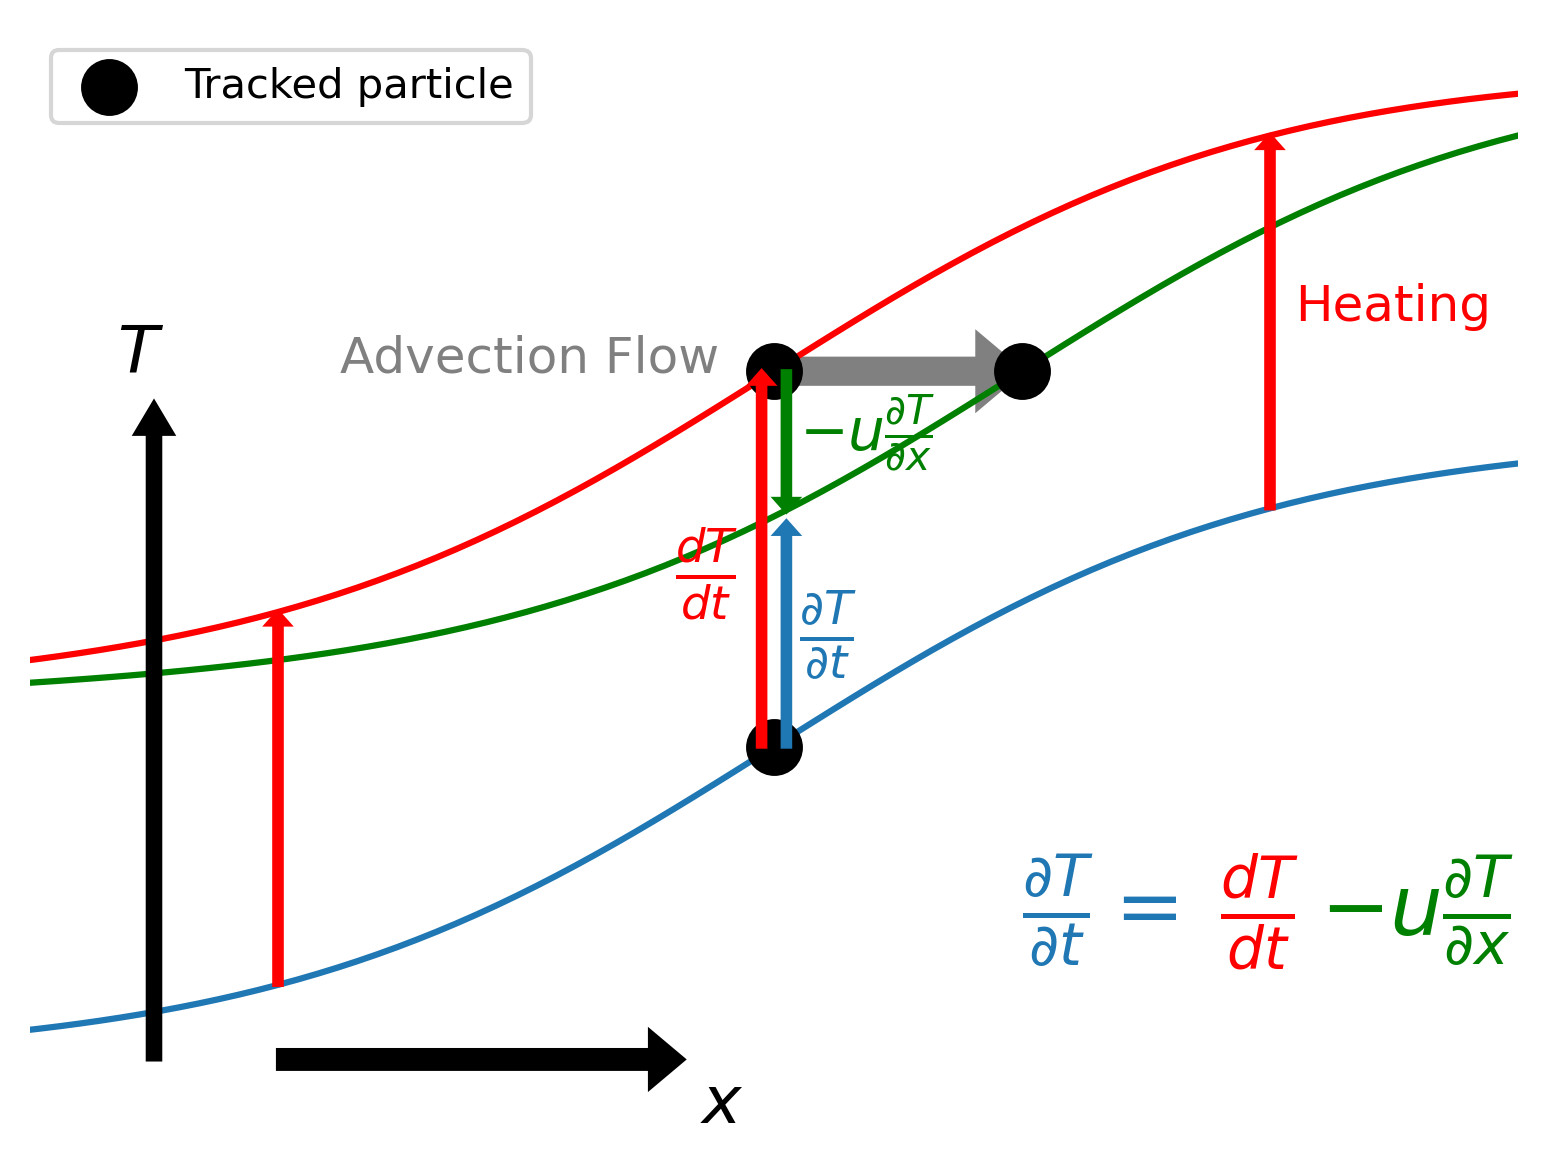
\includegraphics[scale=0.8]{graphics/advect.png}
    \caption{The relationship between the spatial (blue) and material derivative (red) alongside the advective term (green), where we use temperature $T$ as the variable and only look at a single direction $x$ (and velocity $u$) for demonstration.}
    \label{fig:advection}
\end{figure}

\subsection{Field Equations}
In this subsection, we will proceed to derive several \index{Field Equations}\keywordhl{field equations} which govern the dynamics of physical fields like temperature and motion. The central ingredient for the derivation is the \textit{conservation of mass}, and we will consider the mass contained in a volume bounded by an arbitrary closed surface. The boundary of this volume will be assumed to move alongside the particles on it and thus it is a \index{Material Volume}\keywordhl{material volume}. Therefore, it will contain the same set of particles for all time. Considering this material volume, the amount of mass inside it can be expressed as an integral over the deformed volume in the current configuration as
\begin{align}
m = \int_{V(t)} \rho(\textbf{x},t) dV \label{eqn:eulermass}
\end{align}
where $V(t)$ represents the current volume and $\rho(\textbf{x},t)$ is the density field in the Eulerian frame, both of which can change with time. However, we can also switch to the Lagrangian frame where the mass integral is taken over a fixed reference volume $V_0 = V(t_0)$, which coincides with the material volume of the mass at some reference time. Moreover, at the reference time, the density will no longer depend on time and will only vary in the reference coordinates, i.e.\ $\rho_0 = \rho_0(\textbf{X}) = \rho(\textbf{x}(\textbf{X},t_0), t_0)$. Therefore, an alternative form of the mass integral will be
\begin{align}
m = \int_{V_0} \rho_0(\textbf{X}) dV_0 \label{eqn:lagmass}
\end{align}
The principle of \index{Conservation of Mass}\keywordhl{conservation of mass} requires that mass can neither be created nor destroyed and thus the mass within a material volume will remain the same at any time. As a result, the rate of change in mass must vanish, i.e. $dm/dt = 0$. Using this on (\ref{eqn:eulermass}) then leads to
\begin{align}
\frac{d}{dt}(\int_{V(t)} \rho(\textbf{x},t) dV) = 0
\end{align}
The problem with this formulation is that the integration volume, in addition to the density, depends on the time and the computation will be difficult. However, we can carry out a coordinate transformation from the Eulerian to the Lagrangian frame by (\ref{eqn:dVJdV_0}) to convert the integral from a moving volume to a reference volume as
\begin{align}
\frac{d}{dt}\left(\int_{V_0} \rho(\textbf{x}(\textbf{X},t),t) JdV_0 \right) = 0 \label{eqn:eulermassdt}   
\end{align}
Compared to (\ref{eqn:lagmass}), the density can now change with time as the condition is relaxed using (\ref{eqn:lagtoeuler}) to compute the current density using the reference coordinates. To proceed, we would like to do the time derivative under the integral sign and this requires us to know how to evaluate $dJ/dt$ first, which is the time derivative of the Jacobian. The Jacobian as a determinant, can be expressed in the Index Notation
\begin{align}
J = \epsilon_{ijk} \frac{\partial x_1}{\partial X_i}\frac{\partial x_2}{\partial X_j}\frac{\partial x_3}{\partial X_k} \label{eqn:Jdefn}
\end{align}
via (\ref{eqn:determinanteps3}) where $\partial x_l/\partial X_i$ is the Jacobian in the matrix/tensor form. Since the partial derivatives in the Jacobian are defined with respect to the material reference coordinates, the time derivative of the Jacobian can be done directly. Using the Product Rule, we have
\begin{align}
\frac{dJ}{dt} =  \epsilon_{ijk} [\frac{d}{dt}(\frac{\partial x_1}{\partial X_i})\frac{\partial x_2}{\partial X_j}\frac{\partial x_3}{\partial X_k} +  \frac{\partial x_1}{\partial X_i}\frac{d}{dt}(\frac{\partial x_2}{\partial X_j})\frac{\partial x_3}{\partial X_k} +  \frac{\partial x_1}{\partial X_i}\frac{\partial x_2}{\partial X_j}\frac{d}{dt}(\frac{\partial x_3}{\partial X_k})]
\label{eqn:dJdt1}
\end{align}
Note that in the material coordinates, by (\ref{eqn:lagpartialt}) the time derivative can be treated as a partial derivative, and by \index{Clairaut's Theorem}\keywordhl{Clairaut's Theorem} in Multivariable Calculus we can exchange the order of partial derivatives if they are smooth enough. Therefore, we have
\begin{align}
\frac{d}{dt}\frac{\partial x_l}{\partial X_i} = \frac{\partial}{\partial t}\frac{\partial x_l}{\partial X_i} = \frac{\partial}{\partial X_i}\frac{\partial x_l}{\partial t} = \frac{\partial}{\partial X_i}(\frac{d x_l}{dt}) = \frac{\partial v_l}{\partial X_i}
\end{align}
Now, we invoke the Eulerian description and introduce the current coordinates, such that
\begin{align}
\frac{\partial v_l}{\partial X_i} = \frac{\partial v_l}{\partial x_p}\frac{\partial x_p}{\partial X_i}
\end{align}
Take the first term in (\ref{eqn:dJdt1}) to illustrate, it becomes
\begin{align}
\epsilon_{ijk} \frac{d}{dt}(\frac{\partial x_1}{\partial X_i})\frac{\partial x_2}{\partial X_j}\frac{\partial x_3}{\partial X_k} = \epsilon_{ijk} \frac{\partial v_1}{\partial X_i}\frac{\partial x_2}{\partial X_j}\frac{\partial x_3}{\partial X_k} = \epsilon_{ijk} \frac{\partial v_1}{\partial x_p}\frac{\partial x_p}{\partial X_i}\frac{\partial x_2}{\partial X_j}\frac{\partial x_3}{\partial X_k} 
\end{align}
Notice that
\begin{align*}
\epsilon_{ijk} \frac{\partial x_p}{\partial X_i}\frac{\partial x_2}{\partial X_j}\frac{\partial x_3}{\partial X_k}
\end{align*}
will only give the non-zero Jacobian determinant if $p=1$, since when $p=2,3$ the rows of the determinant will be identical and hence
\begin{align}
\epsilon_{ijk} \frac{\partial v_1}{\partial x_p}\frac{\partial x_p}{\partial X_i}\frac{\partial x_2}{\partial X_j}\frac{\partial x_3}{\partial X_k} =  \frac{\partial v_1}{\partial x_1}(\epsilon_{ijk}\frac{\partial x_1}{\partial X_i}\frac{\partial x_2}{\partial X_j}\frac{\partial x_3}{\partial X_k}) = \frac{\partial v_1}{\partial x_1}J
\end{align}
where we have used the definition of $J$ in (\ref{eqn:Jdefn}). We can also show this by writing out the determinants in full as in (\ref{eqn:determinanteps3}):
\begin{align*}
&\quad\epsilon_{ijk} (\frac{\partial v_1}{\partial x_p}\frac{\partial x_p}{\partial X_i})\frac{\partial x_2}{\partial X_j}\frac{\partial x_3}{\partial X_k} \\
&= \small\begin{vmatrix}
\dfrac{\partial v_1}{\partial x_p}\dfrac{\partial x_p}{\partial X_1} & \dfrac{\partial v_1}{\partial x_p}\dfrac{\partial x_p}{\partial X_2} & \dfrac{\partial v_1}{\partial x_p}\dfrac{\partial x_p}{\partial X_3} \\[10pt]
\dfrac{\partial x_2}{\partial X_1} & \dfrac{\partial x_2}{\partial X_2} & \dfrac{\partial x_2}{\partial X_3} \\[10pt]
\dfrac{\partial x_3}{\partial X_1} & \dfrac{\partial x_3}{\partial X_2} & \dfrac{\partial x_3}{\partial X_3} 
\end{vmatrix} \\
&= \frac{\partial v_1}{\partial x_1}\small\begin{vmatrix}
\dfrac{\partial x_1}{\partial X_1} & \dfrac{\partial x_1}{\partial X_2} & \dfrac{\partial x_1}{\partial X_3} \\[10pt]
\dfrac{\partial x_2}{\partial X_1} & \dfrac{\partial x_2}{\partial X_2} & \dfrac{\partial x_2}{\partial X_3} \\[10pt]
\dfrac{\partial x_3}{\partial X_1} & \dfrac{\partial x_3}{\partial X_2} & \dfrac{\partial x_3}{\partial X_3} 
\end{vmatrix} +
\frac{\partial v_1}{\partial x_2}\small\begin{vmatrix}
\dfrac{\partial x_2}{\partial X_1} & \dfrac{\partial x_2}{\partial X_2} & \dfrac{\partial x_2}{\partial X_3} \\[10pt]
\dfrac{\partial x_2}{\partial X_1} & \dfrac{\partial x_2}{\partial X_2} & \dfrac{\partial x_2}{\partial X_3} \\[10pt]
\dfrac{\partial x_3}{\partial X_1} & \dfrac{\partial x_3}{\partial X_2} & \dfrac{\partial x_3}{\partial X_3} 
\end{vmatrix} +
\frac{\partial v_1}{\partial x_3}\small\begin{vmatrix}
\dfrac{\partial x_3}{\partial X_1} & \dfrac{\partial x_3}{\partial X_2} & \dfrac{\partial x_3}{\partial X_3} \\[10pt]
\dfrac{\partial x_2}{\partial X_1} & \dfrac{\partial x_2}{\partial X_2} & \dfrac{\partial x_2}{\partial X_3} \\[10pt]
\dfrac{\partial x_3}{\partial X_1} & \dfrac{\partial x_3}{\partial X_2} & \dfrac{\partial x_3}{\partial X_3} 
\end{vmatrix} \\
&= \frac{\partial v_1}{\partial x_1} J + \frac{\partial v_1}{\partial x_2}(0) + \frac{\partial v_1}{\partial x_3} (0) = \frac{\partial v_1}{\partial x_1} J \\
&\quad \text{(Properties \ref{proper:zerodet})}
\end{align*}
By the same reasoning, the second and third terms in (\ref{eqn:dJdt1}) will equal to
$(\partial v_2/\partial x_2)J$ and $(\partial v_3/\partial x_3)J$. So finally (\ref{eqn:dJdt1}) is reduced to simply
\begin{align}
\frac{dJ}{dt} = (\frac{\partial v_1}{\partial x_1} + \frac{\partial v_2}{\partial x_2} + \frac{\partial v_3}{\partial x_3}) J = \frac{\partial v_q}{\partial x_q} J = (\nabla \cdot \textbf{v}) J \label{eqn:dJdtdivv}
\end{align}
which becomes the conservation of mass in Jacobian form. Going back to (\ref{eqn:eulermassdt}), we can take the time derivative inside the integral as the reference volume is independent of time, leading to
\begin{align}
\frac{d}{dt}\left(\int_{V_0} \rho(\textbf{x}(\textbf{X},t),t) JdV_0 \right) &= 0 \nonumber \\
\int_{V_0} \frac{d}{dt}\left(\rho(\textbf{x}(\textbf{X},t),t)J\right) dV_0  &= 0 \nonumber \\
\int_{V_0} (J \frac{d\rho}{dt} + \rho\frac{dJ}{dt}) dV_0 &= 0 \nonumber \\
\int_{V_0} (J \frac{d\rho}{dt} + \rho(\nabla \cdot \textbf{v})J) dV_0 &= 0 &\text{(by (\ref{eqn:dJdtdivv}))} \nonumber \\
\int_{V_0} (\frac{d\rho}{dt} + \rho(\nabla \cdot \textbf{v})) JdV_0 = \int_{V(t)}(\frac{d\rho}{dt} + \rho(\nabla \cdot \textbf{v}))dV &= 0
\end{align}
where we move from the Lagrangian frame back to the Eulerian frame in the last line via (\ref{eqn:dVJdV_0}). Since we can enclose the material volume arbitrarily, the integrand has to be identically zero, and hence the conservation of mass is expressed by the \index{Continuity Equation}\keywordhl{continuity equation}:
\begin{align}
\frac{d\rho}{dt} + \rho(\nabla \cdot \textbf{v}) = 0  \label{eqn:contineqn}
\end{align}
By (\ref{eqn:localmatderiv}), we have the local form of the continuity equation:
\begin{align}
\frac{\partial \rho}{\partial t} + \textbf{v} \cdot \nabla\rho + \rho(\nabla \cdot \textbf{v}) = 0  \nonumber \\
\frac{\partial \rho}{\partial t} + \nabla \cdot(\rho\textbf{v}) = 0 
\end{align}
\footnote{\label{footnote:divsv}$\nabla \cdot(\rho\textbf{v}) = \partial_i(\rho v_i) = v_i(\partial_i\rho) + \rho(\partial_iv_i) =  \textbf{v} \cdot \nabla\rho + \rho(\nabla \cdot \textbf{v})$.}
The physical interpretation of the second term $\nabla \cdot(\rho\textbf{v})$ is the mass flux moving out of a locally fixed volume, which leads to a reduction in the local density via the first term. This can be seen by putting $\nabla \cdot(\rho\textbf{v})$ inside an arbitrary volume integral and use (\ref{eqn:tensdivthm}):
\begin{align}
\int_V \nabla \cdot(\rho\textbf{v}) dV &= \int_V \partial_i(\rho v_i) dV \nonumber \\
&= \int_S \rho v_i n_i dS = \int_S \rho\textbf{v} \cdot \hat{n} dS
\end{align}
The continuity equation can also be cast in the Jacobian form. By multiplying (\ref{eqn:contineqn}) by $J$ and use (\ref{eqn:dJdtdivv}), we have
\begin{align}
\frac{d\rho}{dt}J + \rho(\nabla \cdot \textbf{v})J = \frac{d\rho}{dt}J + \rho\frac{dJ}{dt} = \frac{d(\rho J)}{dt} = 0 \label{eqn:drhoJdt}
\end{align}
With this, we can derive a very powerful result that describes the change of the total amount of a quantity inside a volume, the \index{Reynold's Transport Theorem}\keywordhl{Reynold's Transport Theorem}.
\begin{thm}[Reynold's Transport Theorem]
\label{thm:RTT}
For an \textit{extensive} property $A(\textbf{x},t)$ that is proportional to the mass and hence density $\rho(\textbf{x},t)$, the time derivative of its integral within a material volume can be moved inside and will operate only over the quantity $A(\textbf{x},t)$, that is
\begin{align}
\frac{d}{dt} \int_{V(t)} \rho(\textbf{x},t)A(\textbf{x},t)dV = \int_{V(t)} \rho(\textbf{x},t)\frac{d}{dt}(A(\textbf{x},t))dV \label{eqn:RTT}
\end{align}
\end{thm}
\begin{proof}
We will follow the same logic as in the previous derivation for the conservation of mass by first formulating the integral over a reference volume:
\begin{align}
\frac{d}{dt} \int_{V(t)} \rho(\textbf{x},t)A(\textbf{x},t)dV = \frac{d}{dt} \int_{V_0} \rho(\textbf{x}(\textbf{X},t),t)A(\textbf{x}(\textbf{X},t),t)JdV_0  
\end{align}
And again the time derivative can be moved inside the integral to get
\begin{align}
&\quad \frac{d}{dt} \int_{V_0} \rho(\textbf{x}(\textbf{X},t),t)A(\textbf{x}(\textbf{X},t),t)JdV_0 \nonumber \\
&= \int_{V_0} \frac{d}{dt}(\rho J A) dV_0 \nonumber \\
&= \int_{V_0} \frac{d}{dt}(\rho J)A + \rho J\frac{dA}{dt} dV_0 \nonumber \\
&= \int_{V_0} \rho J\frac{dA}{dt} dV_0 & \text{($\frac{d}{dt}(\rho J) = 0$ by (\ref{eqn:drhoJdt}))}
\end{align}
Finally, by the familiar (\ref{eqn:dVJdV_0}) we can convert back to the current volume: 
\begin{align}
\int_{V_0} \rho \frac{dA}{dt} JdV_0 = \int_{V(t)} \rho(\textbf{x},t)\frac{d}{dt}(A(\textbf{x},t))dV 
\end{align}
so the result is established.
\end{proof}
There are two major variants of Reynold's Transport Theorem. First, consider $G(\textbf{x},t) = \rho A$ as a single quantity, then
\begin{align}
\frac{d}{dt} \int_{V(t)} G(\textbf{x},t) dV &= \int_{V(t)} [\frac{d}{dt}(\rho A) - \frac{d\rho}{dt} A] dV & \text{(Product Rule)} \nonumber \\
&= \int_{V(t)} [\frac{dG}{dt} + \rho (\nabla \cdot \textbf{v}) A] dV & \text{(by (\ref{eqn:contineqn}))} \nonumber \\
&= \int_{V(t)} [\frac{\partial G}{\partial t} + \textbf{v}\cdot\nabla G+ (\nabla \cdot \textbf{v})G] dV & \text{(by (\ref{eqn:localmatderiv}))} \nonumber \\
&= \int_{V(t)} [\frac{\partial G}{\partial t} + \nabla \cdot (G\textbf{v})] dV & \text{(Footnote \ref{footnote:divsv})} \nonumber \\
&= \int_{V(t)} \frac{\partial G}{\partial t} dV + \int_{S(t)} G\textbf{v} \cdot \hat{n}dS &\text{(by (\ref{eqn:divthm}))} \label{eqn:RTTflux}
\end{align}
The two terms on R.H.S. mean the local change of $G$ within the material volume and the spread of $G$ as the boundary expands respectively. They give rise to the net change of $G$ in the material volume. Second, if the volume is not material but a so-called \index{Control Volume}\keywordhl{control volume} (denoted by $CV$) that can itself deform and its boundary will change with time but is independent of the mass, i.e.\ does not follow the particles, then we can treat it as a material volume/surface that coincides with the control volume/surface at time $t$ but the velocity of the boundary is properly replaced. (\ref{eqn:RTTflux}) then becomes
\begin{subequations}
\begin{align}
\frac{d}{dt} \int_{CV(t)} G(\textbf{x},t) dV = \int_{CV(t)} \frac{\partial G}{\partial t} dV + \int_{S(t)} G\textbf{v}_b \cdot \hat{n}dS
\end{align}  
where $\textbf{v}_b$ is the velocity of the control surface. Meanwhile, for the original material volume (now denoted by $MV$), the integral is simply
\begin{align}
\frac{d}{dt} \int_{MV(t)} G(\textbf{x},t) dV = \int_{MV(t)} \frac{\partial G}{\partial t} dV + \int_{S(t)} G\textbf{v}_m \cdot \hat{n}dS
\end{align}  
\end{subequations}
As we demand the material volume to match with the control volume at time $t$, subtracting the first equation from the second one will eliminate the local term, and gives
\begin{align}
\frac{d}{dt} \int_{MV(t)} G(\textbf{x},t) dV &= \frac{d}{dt} \int_{CV(t)} G(\textbf{x},t) dV +  \int_{S(t)} G(\textbf{v}_m - \textbf{v}_b) \cdot \hat{n}dS \nonumber \\
&= \frac{d}{dt} \int_{CV(t)} G(\textbf{x},t) dV + \int_{S(t)} G\textbf{v}_r \cdot \hat{n}dS 
\end{align}
with $\textbf{v}_r = \textbf{v}_m - \textbf{v}_b$ being the relative velocity of the material to control boundary.\par

Now we will use Reynold's Transport Theorem \ref{thm:RTT} to derive the \textit{equation of motion}. Let $A = \textbf{v}$ be the velocity field so that $\rho \textbf{v}$ now represents the momentum per unit mass. The change in the total momentum of a material volume is caused by two major effects: the external traction $\textbf{T}$ on the material boundary and the \textit{body force} (exerted at a distance, per unit mass) $\textbf{b}$ over the entire volume:
\begin{align}
\frac{d}{dt} \int_V \rho \textbf{v} dV = \int_S \textbf{T} dS + \int_V \rho\textbf{b} dV
\end{align}
By the Reynold's Transport Theorem (\ref{eqn:RTT}) and Cauchy's formula (\ref{eqn:Cauchyform}), it becomes
\begin{align}
\int_V \rho \frac{dv_j}{dt} dV = \int_S \sigma_{ij}n_i dS + \int_V \rho b_j dV   
\end{align}
written in the Index Notation. By (\ref{eqn:tensdivthm}), we can rewrite the traction term to obtain
\begin{align}
\int_V \rho \frac{dv_j}{dt} dV &= \int_V \frac{\partial\sigma_{ij}}{\partial x_i} dV + \int_V \rho b_j dV \nonumber \\
\int_V (\rho \frac{dv_j}{dt} - (\frac{\partial\sigma_{ij}}{\partial x_i}+\rho b_j))dV &= 0
\end{align}
Again, as this holds for any material volume, the integrand has to be identically zero, which gives us the desired \index{Equation of Motion}\keywordhl{Equation of Motion}:
\begin{align}
\rho \frac{dv_j}{dt} - (\frac{\partial\sigma_{ij}}{\partial x_i}+\rho b_j) &= 0 \nonumber \\
\rho \frac{dv_j}{dt} &= \frac{\partial\sigma_{ij}}{\partial x_i}+\rho b_j \label{eqn:eqnmotion}
\end{align}
In the ocean or atmosphere, we often assume the fluid is \textit{inviscid} so it cannot support shear stress, although it may be necessary to include viscous forces otherwise. The stress tensor is then reduced to the \textit{hydrostatic pressure} $\sigma_{ij} = -p\delta_{ij}$ which has the same magnitude acting in all directions. Subsequently, (\ref{eqn:eqnmotion}) becomes
\begin{align}
\rho \frac{dv_j}{dt} &= -\frac{\partial (p\delta_{ij})}{\partial x_i} + \rho b_j \nonumber \\
\rho \frac{dv_j}{dt} &= -\frac{\partial p}{\partial x_j} + \rho b_j \implies \rho\frac{d\textbf{v}}{dt} = -\nabla p + \rho \textbf{b} \label{eqn:eqnmotion2}
\end{align}
which are commonly referred to as the \textit{Euler's equations} that can be explicitly expressed in full form for each component:
\begin{subequations}
\begin{empheq}[left={\empheqlbrace}]{alignat=2}
&\rho (\frac{\partial u}{\partial t} + u\frac{\partial u}{\partial x} + v\frac{\partial u}{\partial y} + w\frac{\partial u}{\partial z}) & &= -\frac{\partial p}{\partial x} + \rho g_x \\
&\rho (\frac{\partial v}{\partial t} + u\frac{\partial v}{\partial x} + v\frac{\partial v}{\partial y} + w\frac{\partial v}{\partial z}) & &= -\frac{\partial p}{\partial y} + \rho g_y \\
&\rho (\frac{\partial w}{\partial t} + u\frac{\partial w}{\partial x} + v\frac{\partial w}{\partial y} + w\frac{\partial w}{\partial z}) & &= -\frac{\partial p}{\partial z} + \rho g_z
\end{empheq} 
\end{subequations}
where we denote the three-dimensional flow velocities as $\textbf{v} = (u,v,w)^T$, the body force is the gravity $\textbf{b} = \textbf{g} = (g_x,g_y,g_z)^T$, and use (\ref{eqn:localmatderiv}) to expand the material time derivative. Note that we are doing the above analysis in a non-rotating inertial coordinate frame so the usual Coriolis force does not appear.\par

Finally, we will use Euler's equations to derive \index{Kelvin's Circulation Theorem}\keywordhl{Kelvin's Circulation Theorem}. \textit{Circulation} along a closed material path is the line integral of velocity along it:
\begin{align}
\Gamma_c = \oint_{C(t)} v_i dx_i
\end{align}
Its time derivative is 
\begin{align}
\frac{d\Gamma_c}{dt} &= \frac{d}{dt}(\oint_{C} v_i dx_i) \nonumber \\
&= \oint_{C} \frac{d}{dt}(v_i dx_i)  \nonumber \\\
&\quad \begin{aligned}
&\text{(Take the material derivative inside and enclose the material} \\  
&\text{line elements to account for the moving material loop)} 
\end{aligned} \nonumber \\
&= \oint_{C} \frac{dv_i}{dt} dx_i + \oint_{C} v_i d(\frac{dx_i}{dt})  \nonumber \\
&\quad \begin{aligned}
&\text{(Material line elements move with the flow and thus} \\ 
&\frac{d}{dt}(dx_i) = d(\frac{dx_i}{dt})\text{)}\end{aligned} \nonumber \\
&= \oint_{C} \frac{dv_i}{dt} dx_i + \oint_{C} v_i dv_i \nonumber \\
&= \oint_{C} \frac{dv_i}{dt} dx_i + \oint_{C} d(\frac{\norm{\textbf{v}}^2}{2}) 
\end{align}
The second integral is zero because the value of a scalar in a closed path must be unchanged after a loop. Substitute (\ref{eqn:eqnmotion2}) into the first integral yields
\begin{align*}
\oint_{C} \frac{dv_i}{dt} dx_i &= \oint_{C} (-\frac{1}{\rho}\frac{\partial p}{\partial x_i} + g_i) dx_i \\
&= - \oint_{C} \frac{1}{\rho}\frac{\partial p}{\partial x_i} dx_i + \oint_{C} g_i dx_i \\
&= - \oint_C \frac{dp}{\rho} + (0)
\end{align*}
where the second smaller integral vanishes because gravity is treated as a constant vector and the closed path integral will cancel out itself and Kelvin's Circulation Theorem is established:
\begin{align}
\frac{d\Gamma_c}{dt} &= - \oint_C \frac{dp}{\rho}  
\end{align}
Another form of the theorem is
\begin{align}
\frac{d\Gamma_c}{dt} &= \int_S \frac{\nabla \rho \times \nabla p}{\rho^2} \cdot \hat{n} dS     
\end{align}
due to Stokes's Theorem adapted from (\ref{eqn:stokes})\footnote{We reduce the conversion of integrals to that between a curve and surface. For a vector field $\textbf{u}$, denote the normal vectors to the surface element and line element as $\textbf{n}$ and $\textbf{m}$ respectively, and the tangential unit vector as $\textbf{t}$, then $\textbf{n} \times \textbf{m} = \textbf{t}$ and (\ref{eqn:tensdivthm}) can be appropriately turned into
\begin{align*}
\int_S (\nabla \times \textbf{u}) \cdot \hat{n} dS &= \int_S \epsilon_{ijk}\partial_j u_k n_i dS \\
&= \oint_C \epsilon_{ijk} u_k n_i m_j dl \\
&= \oint_C u_k (\epsilon_{kij} n_i m_j) dl = \oint_C u_k t_k dl \\
&= \oint_C u_k dl_k = \oint_C \textbf{u} \cdot d\textbf{l}
\end{align*}
Now take $\textbf{u} = \nabla p/\rho$.}:
\begin{align*}
- \oint_C \frac{dp}{\rho} &= - \oint_C \frac{\nabla p \cdot dl}{\rho} \\
&= - \int_S \nabla \times (\frac{\nabla p}{\rho}) \cdot \hat{n} dS \\
&= \int_S  \frac{\nabla \rho \times \nabla p}{\rho^2} \cdot \hat{n} dS     
\end{align*}
\footnote{By Product Rule, \begin{align*}
\nabla \times (\frac{\nabla p}{\rho}) &= \epsilon_{ijk}\partial_j(\frac{\partial_k p}{\rho}) \\
&= \epsilon_{ijk}(\frac{\partial_j\partial_k p}{\rho}) + \epsilon_{ijk}(-\frac{\partial_k p}{\rho^2})\partial_j\rho
\end{align*}
The first term is the zero vector since the partial derivatives are symmetric but the epsilon symbol is antisymmetric:
\vspace{\maxdimen}
\begin{align*}
\epsilon_{ijk}(\frac{\partial_j\partial_k p}{\rho}) &= \epsilon_{ikj}(\frac{\partial_k\partial_j p}{\rho}) \\
&= -\epsilon_{ijk}(\frac{\partial_k\partial_j p}{\rho}) = -\epsilon_{ijk}(\frac{\partial_j\partial_k p}{\rho}) \implies \epsilon_{ijk}(\frac{\partial_j\partial_k p}{\rho}) = \textbf{0}
\end{align*}
and the second term leads to
\begin{align*}
-\epsilon_{ijk}(\frac{\partial_k p}{\rho^2})\partial_j\rho = -\epsilon_{ijk}\frac{\partial_j\rho \partial_k p}{\rho^2} = -\frac{\nabla \rho \times \nabla p}{\rho^2}
\end{align*}
}
The quantity 
\begin{align}
\frac{\nabla \rho \times \nabla p}{\rho^2}    
\end{align}
is called the \textit{baroclinicity} which characterizes the tilting between the pressure/density contours. It often arises from a temperature gradient in a cross-section, which will generate circulation along the corresponding curve.

\section{Earth System Applications: Data Assimilation}

\subsection{Basic Ideas behind Data Assimilation}

\index{Data Assimilation}\keywordhl{Data Assimilation (DA)} is a technique to integrate current \textit{observations} into the \textit{background} state of a weather model to produce a more accurate \textit{analysis} field. This is needed as the error of the model will inevitably grow in time and become useless if it is not supplied with real information. To motivate, we will use air temperature at a fixed grid point as a single variable (\textit{univariate}) example. Let the true temperature be $T_t$, and the background temperature from the model output be
\begin{subequations}
\begin{align}
T_b = T_t + \varepsilon_b \label{eqn:backgT}
\end{align}    
where $\varepsilon_b$ is the background error with a variance of
\begin{align}
E[\varepsilon_b^2] = \sigma_b^2
\end{align}
The variance here is formulated by integrating over the \textit{probability distribution function (PDF)} and is a generalization of that in Definition \ref{defn:variance}.
\end{subequations}
Similarly, the observation temperature is
\begin{subequations}
\begin{align}
T_o = T_t + \varepsilon_o \label{eqn:obsT}
\end{align}    
and the observation error has a variance of
\begin{align}
E[\varepsilon_o^2] = \sigma_o^2
\end{align}
\end{subequations}
Further, we assume that they are \textit{unbiased} such that
\begin{subequations}
\label{eqn:unbiasedbo}
\begin{align}
E[T_b] &= T_t &  \text{or} & & E[\varepsilon_b] &= 0 \\
E[T_o] &= T_t &  \text{or} & & E[\varepsilon_o] &= 0
\end{align}
\end{subequations}
Moreover, the background and observation errors have to be \textit{uncorrelated}:
\begin{align}
E[\varepsilon_b\varepsilon_o] &= 0 \label{eqn:bouncorr}
\end{align}
We set out to find an optimal linear combination of $T_b$ and $T_o$ as a new unbiased estimation, referred to as the \textit{analysis}:
\begin{align}
T_a = a_1T_b + a_2T_o \label{eqn:analysisT}
\end{align}
where $a_1, a_2 > 0$ are the weights. The analysis will also have an error of $\varepsilon_a$ such that 
\begin{align}
T_a = T_t + \varepsilon_a
\end{align}
The condition of being unbiased requires that
\begin{align}
E[\varepsilon_a] = E[T_a - T_t] &= 0 \nonumber \\
E[a_1T_b + a_2T_o - T_t] &= 0 \nonumber &\text{(By (\ref{eqn:analysisT}))}\\
E[a_1(T_t + \varepsilon_b) + a_2(T_t + \varepsilon_o) - T_t] &= 0 \nonumber\\
\text{(By (\ref{eqn:backgT}) and (\ref{eqn:obsT}))} &\nonumber \\
a_1(E[T_t] + E[\varepsilon_b]) + a_2(E[T_t] + E[\varepsilon_o]) - E[T_t] &= 0 \nonumber \\
(a_1 + a_2 - 1)E[T_t] &= 0 &\text{(By (\ref{eqn:unbiasedbo}))} \nonumber \\
\implies a_1 + a_2 &= 1
\end{align}
i.e.\ the sum of weighting has to be unity ($1$). To obtain the best analysis estimation $T_a$, we want the weighting to minimize the mean squared error of $T_a$, a.k.a.\ the analysis error variance 
\begin{align}
\sigma_a^2 = E[\varepsilon_a^2] = E[(T_a - T_t)^2]
\end{align}
We proceed by differentiating it with respect to one of the weights, let's say $a_1$, and the minimum will occur when the partial derivative is zero:
\begin{align}
\frac{\partial \sigma_a^2}{\partial a_1} &= 0 \label{eqn:DAunimin}
\end{align}
Now
\begin{align}
\varepsilon_a = T_a - T_t &= a_1T_b + a_2T_o - (a_1 + a_2)T_t & \text{($a_1 + a_2 = 1$)}\nonumber \\
&= a_1(T_b-T_t) + a_2(T_o-T_t) \nonumber \\
&= a_1\varepsilon_b + a_2\varepsilon_o
\end{align}
and hence
\begin{align}
\sigma_a^2 = E[\varepsilon_a^2] &= E[(T_a - T_t)^2] \nonumber \\
&= E[(a_1\varepsilon_b + a_2\varepsilon_o)^2] \nonumber \\
&= E[a_1^2\varepsilon_b^2 + a_1a_2\varepsilon_b\varepsilon_o + a_2^2\varepsilon_o^2] \nonumber \\
&= a_1^2E[\varepsilon_b^2] + a_1a_2 E[\varepsilon_b\varepsilon_o] + a_2^2E[\varepsilon_o^2] \nonumber \\
&= a_1^2\sigma_b^2 + a_2^2\sigma_o^2 & \text{(By (\ref{eqn:bouncorr}))} \nonumber \\
&= a_1^2\sigma_b^2 + (1-a_1)^2\sigma_o^2 \label{eqn:DAunisigmaa}
\end{align}
Substituting this into (\ref{eqn:DAunimin}), we obtain
\begin{align}
\frac{\partial \sigma_a^2}{\partial a_1} = \frac{\partial}{\partial a_1}(a_1^2\sigma_b^2 + (1-a_1)^2\sigma_o^2) &= 0 \nonumber \\
2a_1\sigma_b^2 - 2(1-a_1)\sigma_o^2 &= 0 \nonumber \\
2a_1(\sigma_b^2 + \sigma_o^2) - 2\sigma_o^2 &= 0 \nonumber \\
a_1 &= \frac{\sigma_o^2}{\sigma_b^2 + \sigma_o^2} = \frac{\sigma_b^{-2}}{\sigma_b^{-2} + \sigma_o^{-2}}
\end{align}
where the second equality in the last line is from dividing by \smash{$\sigma_b^2\sigma_o^2$}. The reciprocals of the background/observation error variances \smash{$\sigma_b^{-2}, \sigma_o^{-2}$} represent their respective \textit{precisions}. The best analysis is then given by
\begin{align}
T_a &= a_1T_b + (1-a_1)T_o \nonumber \\
&= \frac{\sigma_o^2}{\sigma_b^2 + \sigma_o^2}T_b + \frac{\sigma_b^2}{\sigma_b^2 + \sigma_o^2}T_o =  \frac{\sigma_b^{-2} T_b + \sigma_o^{-2} T_o}{\sigma_b^{-2} + \sigma_o^{-2}} \label{eqn:univOIan}
\end{align}
Therefore, the analysis is a weighted average of the background and the observation where the weights are proportional to their precisions. The analysis error variance in (\ref{eqn:DAunisigmaa}) is subsequently
\begin{align}
\sigma_a^2 &= a_1^2\sigma_b^2 + (1-a_1)^2\sigma_o^2 \nonumber \\
&= (\frac{\sigma_o^2}{\sigma_b^2 + \sigma_o^2})^2\sigma_b^2 + (\frac{\sigma_b^2}{\sigma_b^2 + \sigma_o^2})^2\sigma_o^2 \nonumber \\
&= \frac{\sigma_b^2\sigma_o^2(\sigma_b^2 + \sigma_o^2)}{(\sigma_b^2 + \sigma_o^2)^2} \nonumber \\
&= \frac{\sigma_b^2\sigma_o^2}{\sigma_b^2 + \sigma_o^2} = \frac{1}{\sigma_b^{-2} + \sigma_o^{-2}} \label{eqn:DAunisigmaa2}
\end{align}
or alternatively,
\begin{align}
\frac{1}{\sigma_a^2} = \frac{1}{\sigma_b^2} + \frac{1}{\sigma_o^2}
\end{align}
which means that the precision of the analysis is the sum of the precisions of
the background and observation. An illustration is given in Figure \ref{fig:DA1} below. By rearranging the expressions in (\ref{eqn:univOIan}) and (\ref{eqn:DAunisigmaa2}), the data assimilation prototype is described by
\begin{subequations}
\label{eqn:univOIschm}
\begin{align}
W &= \frac{\sigma_b^2}{\sigma_b^2 + \sigma_o^2}\\  
T_a &= T_b + W(T_o - T_b) \label{eqn:uniDAweight} \\
\sigma_a^2 &= (1 - W)\sigma_b^2
\end{align}    
\end{subequations}

\begin{figure}[ht!]
    \centering
    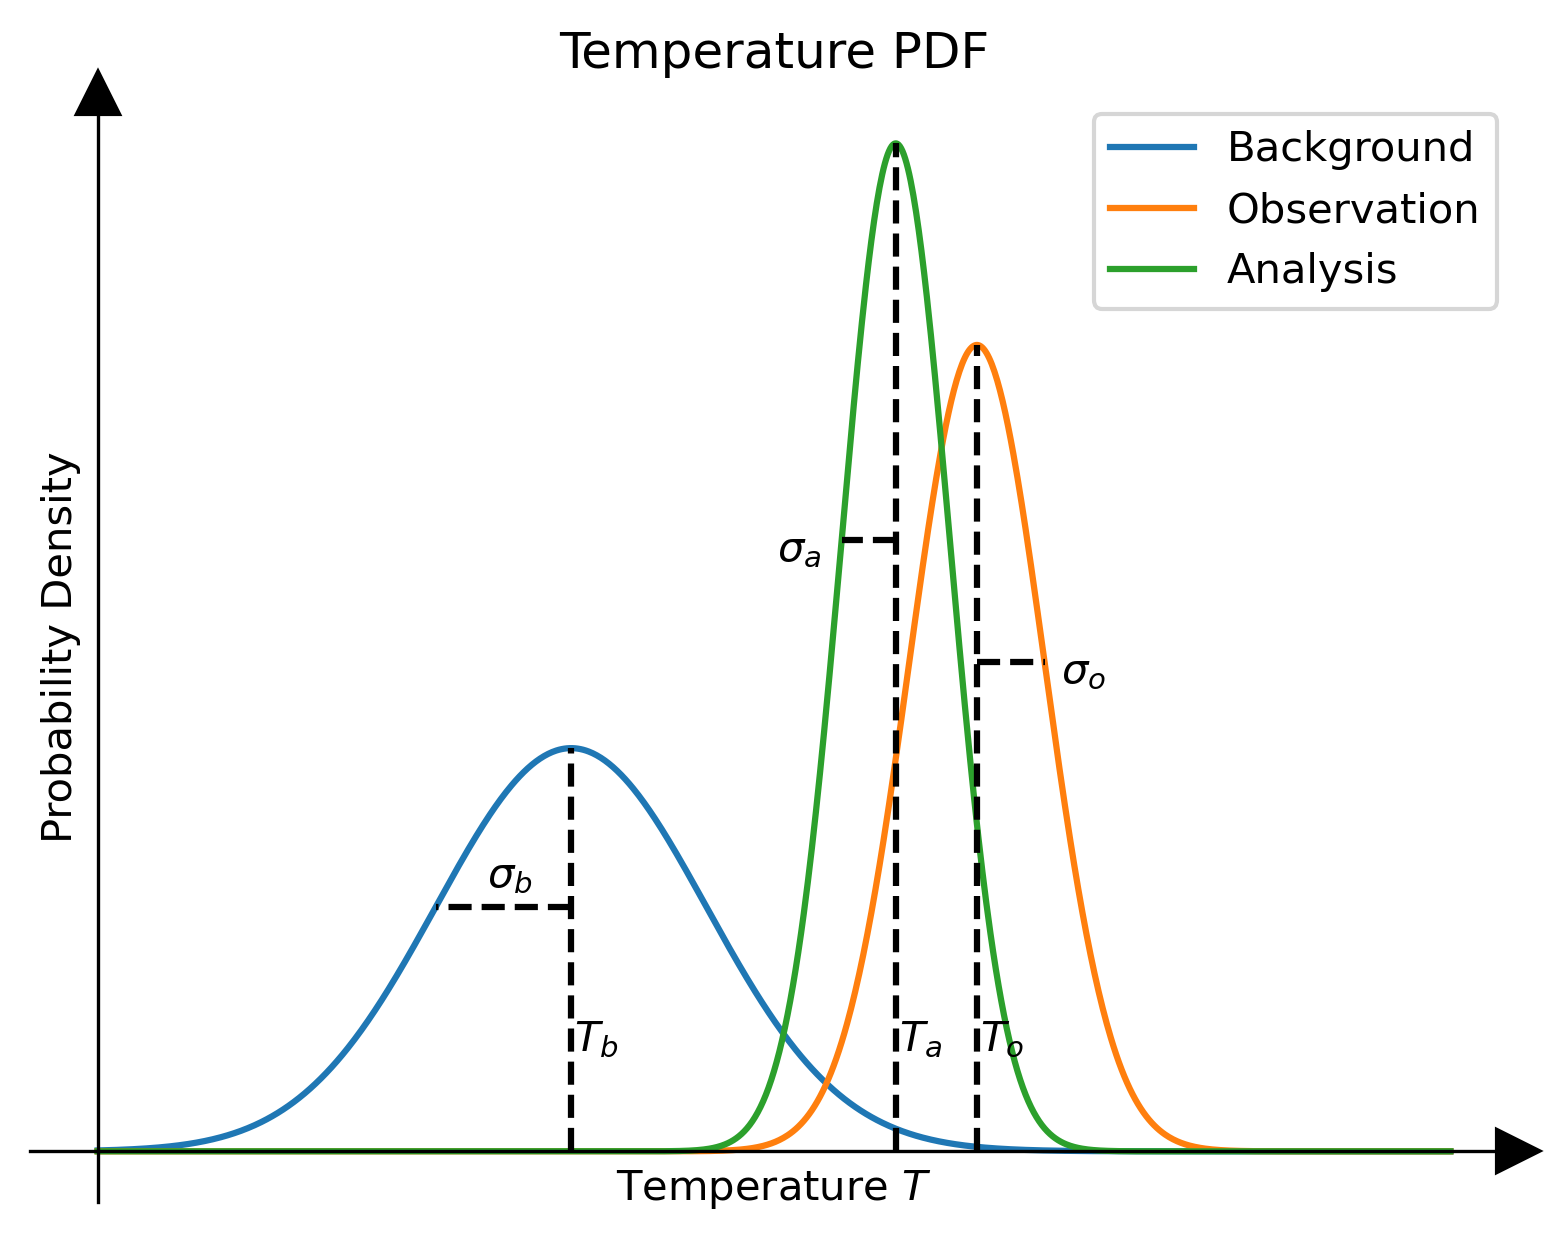
\includegraphics[scale=0.75]{graphics/DA1.png}
    \caption{The probability density distribution of the background/observation/analysis temperatures in the section example where the errors are assumed to have a Gaussian shape.}
    \label{fig:DA1}
\end{figure}

\subsection{Optimal Interpolation}

In the last subsection, we only use a single variable as the illustrating example. Obviously, in actual weather models, there will be multiple variables (let's say $N$) like temperature, pressure, density, and three-dimensional winds to be simulated in a large number of grid points ($M$). Hence there will be a total of $L = MN$ variables in the model output and we will place all of them into a \textit{state vector} of length $L = MN$:
\begin{align}
\textbf{x} = 
\begin{bmatrix}
x_1 \\
x_2 \\
\vdots \\
x_L
\end{bmatrix}
\end{align}
with a corresponding error vector of
\begin{align}
\bm{\epsilon} =  
\begin{bmatrix}
\varepsilon_1 \\
\varepsilon_2 \\
\vdots \\
\varepsilon_L
\end{bmatrix}
\end{align}
which is assumed to be unbiased too, such that the expected values of the errors $E(\bm{\epsilon}) = \textbf{0}$ is always a zero vector. The \textit{error covariance matrix} is then defined as
\begin{align}
P &= E[(\bm{\epsilon} - E(\bm{\epsilon}))(\bm{\epsilon} - E(\bm{\epsilon}))^T] = E[\bm{\epsilon}\bm{\epsilon}^T] \nonumber \\
&= \begin{bmatrix}
E[\varepsilon_1\varepsilon_1] & E[\varepsilon_1\varepsilon_2] & \cdots & E[\varepsilon_1\varepsilon_L] \\
E[\varepsilon_2\varepsilon_1] & E[\varepsilon_2\varepsilon_2] & & E[\varepsilon_1\varepsilon_L] \\
\vdots & & \ddots & \vdots \\
E[\varepsilon_L\varepsilon_1] & E[\varepsilon_L\varepsilon_2] & \cdots & E[\varepsilon_L\varepsilon_L] 
\end{bmatrix}
\end{align}
which is generalized from Properties \ref{proper:variancemul}. We will start with the simplest case where the observations are exactly the model variables. Then the background, analysis, and observation states can be expressed as
\begin{subequations}
\label{eqn:OIxbaoe}
\begin{align}
\textbf{x}_b = \textbf{x}_t + \bm{\epsilon}_b \\
\textbf{x}_a = \textbf{x}_t + \bm{\epsilon}_a \\
\textbf{x}_o = \textbf{x}_t + \bm{\epsilon}_o
\end{align}    
\end{subequations}
relative to the truth $\textbf{x}_t$. The error covariance matrices for the background, analysis, and observation are
\begin{subequations}
\label{eqn:OIPmat}
\begin{align}
P_b &= B = E[\bm{\epsilon}_b\bm{\epsilon}_b^T] \\
P_a &= A = E[\bm{\epsilon}_a\bm{\epsilon}_a^T] \\
P_o &= R = E[\bm{\epsilon}_o\bm{\epsilon}_o^T]
\end{align}    
\end{subequations}
As before, we assume that the background and observation errors are uncorrelated so that
\begin{align}
E[\bm{\epsilon}_b\bm{\epsilon}_o^T] = E[\bm{\epsilon}_o\bm{\epsilon}_b^T] = \textbf{0} \label{eqn:OIuncorr}
\end{align}
We also require the analysis $\textbf{x}_a$ to be an unbiased linear combination of $\textbf{x}_b$ and $\textbf{x}_o$. This allows us to write
\begin{align}
\textbf{x}_a &= \textbf{x}_b + K(\textbf{x}_o - \textbf{x}_b)  \label{eqn:OIinnov}
\end{align}
akin to (\ref{eqn:uniDAweight}) where $K$ is the \textit{Kalman gain} matrix that represents the optimal weight. Therefore, the analysis will be the background plus the optimal weight times the observation increment (\textit{innovation}). Subsequently,
\begin{align}
\textbf{x}_t + \bm{\epsilon}_a &= \textbf{x}_t + \bm{\epsilon}_b + K(\textbf{x}_o - \textbf{x}_t - \bm{\epsilon}_b) \nonumber \\
\bm{\epsilon}_a &= \bm{\epsilon}_b + K(\bm{\epsilon}_o - \bm{\epsilon}_b) \label{eqn:varakalman}
\end{align}
The total error variance $E[\bm{\epsilon}_a^T\bm{\epsilon}_a]$, or equivalently the trace of $A$, by Index Notation, is
\begin{align}
E[\bm{\epsilon}_a^T\bm{\epsilon}_a] = E[(\varepsilon_a)_i(\varepsilon_a)_i)]  
\end{align}
Similar to (\ref{eqn:DAunimin}), we want to differentiate this quantity but with respect to the Kalman gain matrix $K$ and demand that
\begin{align}
\frac{\partial E[\bm{\epsilon}_a^T\bm{\epsilon}_a]}{\partial K} = E\left(\frac{\partial [\bm{\epsilon}_a^T\bm{\epsilon}_a]}{\partial K}\right) = [\textbf{0}] \label{eqn:Kalmande0}
\end{align}
To proceed, we first note that it works very much like (\ref{eqn:dxdxdelta}) but with two Kronecker deltas now:
\begin{align}
\frac{\partial K_{ij}}{\partial K_{pq}} = \delta_{ip}\delta_{jq}
\end{align}
Now, writing out the subscripts in (\ref{eqn:varakalman}), we have
\begin{align}
(\varepsilon_a)_i(\varepsilon_a)_i = [(\varepsilon_b)_i + K_{ij}((\varepsilon_o)_j - (\varepsilon_b)_j)][(\varepsilon_b)_i + K_{ik}((\varepsilon_o)_k - (\varepsilon_b)_k)]
\end{align}
where we have to use two different dummy indices for the product due to the rule of Index Notation. Then the derivative is computed to be
\begin{align}
&\quad \frac{\partial [\bm{\epsilon}_a^T\bm{\epsilon}_a]}{\partial K} \nonumber \\
&= \frac{\partial}{\partial K_{pq}}\left([(\varepsilon_b)_i + K_{ij}((\varepsilon_o)_j - (\varepsilon_b)_j)][(\varepsilon_b)_i + K_{ik}((\varepsilon_o)_k - (\varepsilon_b)_k)]\right) \nonumber \\
&= \left(\frac{\partial}{\partial K_{pq}}[(\varepsilon_b)_i + K_{ij}((\varepsilon_o)_j - (\varepsilon_b)_j)]\right)[(\varepsilon_b)_i + K_{ik}((\varepsilon_o)_k - (\varepsilon_b)_k)] \nonumber \\
&\quad +[(\varepsilon_b)_i + K_{ij}((\varepsilon_o)_j - (\varepsilon_b)_j)] \left(\frac{\partial}{\partial K_{pq}}[(\varepsilon_b)_i + K_{ik}((\varepsilon_o)_k - (\varepsilon_b)_k)]\right) \nonumber \\
&= \delta_{ip}\delta_{jq}((\varepsilon_o)_j - (\varepsilon_b)_j)[(\varepsilon_b)_i + K_{ik}((\varepsilon_o)_k - (\varepsilon_b)_k)] \nonumber \\
&\quad + ((\varepsilon_b)_i + K_{ij}((\varepsilon_o)_j - (\varepsilon_b)_j)) \delta_{ip}\delta_{kq} ((\varepsilon_o)_k - (\varepsilon_b)_k) \nonumber \\
&= ((\varepsilon_o)_q - (\varepsilon_b)_q)[(\varepsilon_b)_p + K_{pk}((\varepsilon_o)_k - (\varepsilon_b)_k)] \nonumber \\
&\quad + ((\varepsilon_b)_p + K_{pj}((\varepsilon_o)_j - (\varepsilon_b)_j)) ((\varepsilon_o)_q - (\varepsilon_b)_q) \nonumber \\
&= 2((\varepsilon_b)_p + K_{pk}((\varepsilon_o)_k - (\varepsilon_b)_k)) ((\varepsilon_o)_q - (\varepsilon_b)_q) \nonumber \\
&\quad \text{(One of the dummy indices can be changed and the terms will be grouped)} \nonumber \\
&= 2(\varepsilon_b)_p ((\varepsilon_o)_q - (\varepsilon_b)_q) + 2 K_{pk}((\varepsilon_o)_k - (\varepsilon_b)_k)((\varepsilon_o)_q - (\varepsilon_b)_q) \nonumber \\
&= 2 \bm{\epsilon}_b (\bm{\epsilon}_o - \bm{\epsilon}_b)^T + 2K(\bm{\epsilon}_o - \bm{\epsilon}_b)(\bm{\epsilon}_o - \bm{\epsilon}_b)^T \label{eqn:Kalmande0res}
\end{align}
where in the last step we convert it back to matrix form. Plugging it into (\ref{eqn:Kalmande0}) gives the desired expression for the Kalman gain matrix.
\begin{align}
E\left(\frac{\partial [\bm{\epsilon}_a^T\bm{\epsilon}_a]}{\partial K}\right) = E[2 \bm{\epsilon}_b (\bm{\epsilon}_o - \bm{\epsilon}_b)^T + 2K(\bm{\epsilon}_o - \bm{\epsilon}_b)(\bm{\epsilon}_o - \bm{\epsilon}_b)^T] &= [\textbf{0}] \nonumber \\
E[\bm{\epsilon}_b\bm{\epsilon}_o^T] - E[\bm{\epsilon}_b\bm{\epsilon}_b^T] + K(E[\bm{\epsilon}_o\bm{\epsilon}_o^T] - E[\bm{\epsilon}_b\bm{\epsilon}_o^T] - E[\bm{\epsilon}_o\bm{\epsilon}_b^T] + E[\bm{\epsilon}_b\bm{\epsilon}_b^T)] &= [\textbf{0}] \nonumber \\
- E[\bm{\epsilon}_b\bm{\epsilon}_b^T] + K(E[\bm{\epsilon}_o\bm{\epsilon}_o^T] + E[\bm{\epsilon}_b\bm{\epsilon}_b^T]) &= [\textbf{0}] \nonumber \\
\text{(Uncorrelated errors by (\ref{eqn:OIuncorr}))} & \nonumber \\
- B + K(B+R) &= [\textbf{0}] \nonumber \\
\implies K = B(B+R)&^{-1} \label{eqn:OImatK}
\end{align}
The analysis covariance is
\begin{align}
A &= E[\bm{\epsilon}_a\bm{\epsilon}_a^T] \nonumber \\
&= E[(\bm{\epsilon}_b + K(\bm{\epsilon}_o - \bm{\epsilon}_b))(\bm{\epsilon}_b + K(\bm{\epsilon}_o - \bm{\epsilon}_b))^T] \nonumber \\
&= E[\bm{\epsilon}_b\bm{\epsilon}_b^T] + E[\bm{\epsilon}_bK(\bm{\epsilon}_o - \bm{\epsilon}_b)^T] \nonumber \\
&\quad + E[K(\bm{\epsilon}_o - \bm{\epsilon}_b)\bm{\epsilon}_b^T] + E[K(\bm{\epsilon}_o - \bm{\epsilon}_b)(K(\bm{\epsilon}_o - \bm{\epsilon}_b))^T] \nonumber \\
&= E[\bm{\epsilon}_b\bm{\epsilon}_b^T] + E[\bm{\epsilon}_b(\bm{\epsilon}_o - \bm{\epsilon}_b)^TK^T] \nonumber \\
&\quad + E[K(\bm{\epsilon}_o - \bm{\epsilon}_b)\bm{\epsilon}_b^T] + E[K(\bm{\epsilon}_o - \bm{\epsilon}_b) (\bm{\epsilon}_o - \bm{\epsilon}_b)^TK^T] \nonumber \\
&= B - BK^T - KB + K(B+R)K^T \qquad \text{(Uncorrelated errors by (\ref{eqn:OIuncorr}))} \nonumber \\
&= B - BK^T - KB + B(B+R)^{-1} (B+R)K^T \qquad \text{(by (\ref{eqn:OImatK}))} \nonumber \\
&= B - BK^T - KB + BK^T = B - KB = (I-K)B \label{eqn:OIAnalysis}
\end{align}
(\ref{eqn:OIinnov}), (\ref{eqn:OImatK}), and (\ref{eqn:OIAnalysis}) then constitute the \textit{multivariate} \index{Optimal Interpolation}\keywordhl{Optimal Interpolation} scheme that can be compared to (\ref{eqn:univOIschm}). An alternative form for $K$ and $A$ can be derived as follows.
\begin{align}
K = B(B+R)^{-1} &= B[(RR^{-1})B+R(B^{-1}B)]^{-1} \nonumber \\
&= B[R(R^{-1} + B^{-1})B]^{-1} \nonumber  \\
&= BB^{-1}(B^{-1} + R^{-1})^{-1}R^{-1} = (B^{-1} + R^{-1})^{-1}R^{-1} \label{eqn:OIKalt}
\end{align}
\begin{align}
A = B - KB &= B - (B^{-1} + R^{-1})^{-1}R^{-1} B \nonumber \\
&= (B^{-1} + R^{-1})^{-1}(B^{-1} + R^{-1})B - (B^{-1} + R^{-1})^{-1} R^{-1} B \nonumber \\
&= (B^{-1} + R^{-1})^{-1} ((B^{-1} + R^{-1})B - R^{-1} B) \nonumber \\
&= (B^{-1} + R^{-1})^{-1} (B^{-1}B + R^{-1}B - R^{-1} B) \nonumber \\
&= (B^{-1} + R^{-1})^{-1} I = (B^{-1} + R^{-1})^{-1} \nonumber \\
\implies A^{-1} &= B^{-1} + R^{-1}
\end{align}
Same as the univariate case, the inverses of covariance matrices represent the precisions and the analysis precision is just the sum of those of the background and observation. \par

However, most of the time, the observations are not exactly the model variables or measured at different locations from the grid points. Let there be $G$ observations stored in a vector $\textbf{y}_o$, and it is related to the model variables by the observation operator $H$ according to $\textbf{y} = H(\textbf{x})$. Then (a) and (b) of (\ref{eqn:OIxbaoe}) remain the same but (c) is now 
\begin{align}
\textbf{y}_o = H(\textbf{x}_t) + \bm{\epsilon}_o \label{eqn:OIinnover}
\end{align}
where $\textbf{y}_o$ and $ \bm{\epsilon}_o$ are vectors of length $G$. Due to the scope limit, we will only discuss the case where the observation operator $H$ is linear and hence a matrix such that
\begin{align}
\textbf{y} = H(\textbf{x}) = H\textbf{x}   
\end{align}
Then the innovation vector will be 
\begin{align}
\textbf{d} &= \textbf{y}_o - H\textbf{x}_b \nonumber \\
&= \textbf{y}_o - H(\textbf{x}_t + \bm{\epsilon}_b) \nonumber \\
&= \textbf{y}_o - H\textbf{x}_t - H\bm{\epsilon}_b \nonumber \\
&= \bm{\epsilon}_o -  H\bm{\epsilon}_b
\end{align}
Similar to the previous formulation, we compute the analysis as the background plus the optimal weight times the innovation:
\begin{align}
\textbf{x}_a &= \textbf{x}_b + K(\textbf{y}_o - H\textbf{x}_b) = \textbf{x}_b + K\textbf{d} \label{eqn:OIinnov1} \\
\textbf{x}_t + \bm{\epsilon}_a &= \textbf{x}_t + \bm{\epsilon}_b + K\textbf{d} \implies \bm{\epsilon}_a = \bm{\epsilon}_b + K\textbf{d} 
\end{align}
We demand the same as in (\ref{eqn:Kalmande0}). However, note that the only difference of the above expression from (\ref{eqn:varakalman}) is that $\textbf{x}_o - \textbf{x}_b$ is replaced by $\textbf{d}$ and (\ref{eqn:Kalmande0res}) simply becomes
\begin{align}
\frac{\partial (\bm{\epsilon}_a^T\bm{\epsilon}_a)}{\partial K} = 2\bm{\epsilon}_b\textbf{d}^T + 2K\textbf{d}\textbf{d}^T
\end{align}
As before, we require the expected value of this derivative to be zero, and hence
\begin{align}
\frac{\partial E[\bm{\epsilon}_a^T\bm{\epsilon}_a]}{\partial K} = E[2\bm{\epsilon}_b\textbf{d}^T + 2K\textbf{d}\textbf{d}^T] &= [\textbf{0}] \nonumber \\
E[\bm{\epsilon}_b(\bm{\epsilon}_o -  H\bm{\epsilon}_b)^T + K(\bm{\epsilon}_o -  H\bm{\epsilon}_b)(\bm{\epsilon}_o -  H\bm{\epsilon}_b)^T] &= [\textbf{0}] \nonumber \\
E[\bm{\epsilon}_b\bm{\epsilon}_b^TH^T] + KE[\bm{\epsilon}_o\bm{\epsilon}_o^T] + KE[H\bm{\epsilon}_b\bm{\epsilon}_b^TH^T] &= [\textbf{0}] \nonumber \\ 
 \text{(Uncorrelated errors by (\ref{eqn:OIuncorr}))} & \nonumber \\
-BH^T + K(R+HBH^T) &= [\textbf{0}] \nonumber \\
\implies K &= BH^T(HBH^T+R)^{-1} \label{eqn:OImatK2}
\end{align}
The analysis covariance is now
\begin{align}
A &= E[\bm{\epsilon}_a\bm{\epsilon}_a^T] \nonumber \\
&= E[(\bm{\epsilon}_b + K(\bm{\epsilon}_o - H\bm{\epsilon}_b))(\bm{\epsilon}_b + K(\bm{\epsilon}_o - H\bm{\epsilon}_b))^T] \nonumber \\
&= E[\bm{\epsilon}_b\bm{\epsilon}_b^T] - E[KH\bm{\epsilon}_b\bm{\epsilon}_b^T] - E[\bm{\epsilon}_b(KH\bm{\epsilon}_b)^T] \nonumber \\
&\quad + E[(K\bm{\epsilon}_o)(K\bm{\epsilon}_o)^T] + E[KH\bm{\epsilon}_b(KH\bm{\epsilon}_b)^T] \nonumber \\
&\quad \text{(Uncorrelated errors by (\ref{eqn:OIuncorr}))} \nonumber \\
&= E[\bm{\epsilon}_b\bm{\epsilon}_b^T] - E[KH\bm{\epsilon}_b\bm{\epsilon}_b^T] - E[\bm{\epsilon}_b\bm{\epsilon}_b^TH^TK^T] \nonumber \\
&\quad + E[K\bm{\epsilon}_o\bm{\epsilon}_o^TK^T] + E[KH\bm{\epsilon}_b\bm{\epsilon}_b^TH^TK^T] \nonumber \\
&= B - KHB - BH^TK^T + KRK^T + KHBH^TK^T \nonumber \\
&= B - KHB - BH^TK^T + K(HBH^T+R)K^T \nonumber \\
&= B - KHB - BH^TK^T + BH^T(HBH^T+R)^{-1}(HBH^T+R)K^T &\text{(by (\ref{eqn:OImatK2}))} \nonumber \\
&= B - KHB - BH^TK^T + BH^TK^T \nonumber \\
&= B - KHB = (I-KH)B \label{eqn:OIcovA}
\end{align}
Similar to (\ref{eqn:OIKalt}), we can express $K$ in an alternative form. We may be tempted to write 
\begin{align*}
K &= BH^T(HBH^T+R)^{-1} \\
&= BH^T[(H^TR^{-1})^{-1}(H^TR^{-1})HBH^T+R(BH^T)^{-1}(BH^T)]^{-1} 
\end{align*}
just like (\ref{eqn:OIKalt}). However, $H$ will be a non-square $G \times L$ matrix, hence $H^TR^{-1}$ and $BH^T$ are also not square, and their inverses are not defined. To proceed, we need the \index{Sherman-Morrison-Woodbury Formula}\keywordhl{Sherman-Morrison-Woodbury Formula}:
\begin{align}
(A + SXC)^{-1} = A^{-1} - A^{-1}S(X^{-1} + CA^{-1}S)^{-1}CA^{-1}
\end{align}
This can be derived by comparing the upper-left block of Properties \ref{proper:schurinv} and \ref{proper:schurinvD} with $D$ replaced by $-X^{-1}$ and $B$ replaced by $S$. Now substitute $A = R$, $S = H$, $X = B$, $C=H^T$ to get
\begin{align}
(HBH^T + R)^{-1} = R^{-1} - R^{-1}H(B^{-1} + H^TR^{-1}H)^{-1}H^T R^{-1}    
\end{align}
Plugging it into (\ref{eqn:OImatK2}), we have
\begin{align}
K &= BH^T(HBH^T+R)^{-1} \nonumber \\
&= BH^T(R^{-1} - R^{-1}H(B^{-1} + H^TR^{-1}H)^{-1}H^T R^{-1}) \nonumber \\
&= BH^TR^{-1} - BH^TR^{-1}H(B^{-1} + H^TR^{-1}H)^{-1}H^T R^{-1} \nonumber \\
&= B(B^{-1} + H^TR^{-1}H)(B^{-1} + H^TR^{-1}H)^{-1}H^TR^{-1} \nonumber \\
&\quad- BH^TR^{-1}H(B^{-1} + H^TR^{-1}H)^{-1}H^T R^{-1} \nonumber \\
&= (B(B^{-1} + H^TR^{-1}H) - BH^TR^{-1}H)(B^{-1} + H^TR^{-1}H)^{-1}H^TR^{-1} \nonumber \\
&= (BB^{-1} + BH^TR^{-1}H - BH^TR^{-1}H)(B^{-1} + H^TR^{-1}H)^{-1}H^TR^{-1} \nonumber \\
&= I(B^{-1} + H^TR^{-1}H)^{-1}H^TR^{-1} = (B^{-1} + H^TR^{-1}H)^{-1}H^TR^{-1}
\end{align}
and the analysis covariance can be rewritten as
\begin{align}
A = B - KHB &= B - (B^{-1} + H^TR^{-1}H)^{-1}H^TR^{-1}HB \nonumber \\
&= (B^{-1} + H^TR^{-1}H)^{-1}(B^{-1} + H^TR^{-1}H)B \nonumber \\
&\quad- (B^{-1} + H^TR^{-1}H)^{-1}H^TR^{-1}HB \nonumber \\
&= (B^{-1} + H^TR^{-1}H)^{-1}((B^{-1} + H^TR^{-1}H)B - H^TR^{-1}HB) \nonumber \\
&= (B^{-1} + H^TR^{-1}H)^{-1}(B^{-1}B + H^TR^{-1}HB - H^TR^{-1}HB) \nonumber \\
&= (B^{-1} + H^TR^{-1}H)^{-1} \implies A^{-1} = B^{-1} + H^TR^{-1}H
\end{align}

\subsection{Kalman Filter}

Notice that the technique of Optimal Interpolation introduced in the last subsection does not depend on time and can be used at any time step in an isolated fashion. However, in physical models, we need to integrate forwards in time for the forecast. We may ask if there is an improved version of Optimal Interpolation such that it will take the evolution of the model state into account. Particularly, the background error is previously assumed to be static but should actually change in time, e.g. different climatologies in different seasons. \index{Kalman Filter}\keywordhl{Kalman Filter} solves this by further cycling the background error covariance using the model. It is essentially Optimal Interpolation but with the error covariances evolved forward in time as well. No matter how the background error is initially determined, it will become more and more optimal after several cycles as long as the model and observations are good. Kalman Filter consists of two steps: the \textit{analysis step} which is identical to Optimal Interpolation, and the \textit{forecast step} where we carry out time integration for the state vector and the error covariance matrix in the model.\par

In Kalman filter, a short-term model forecast is used as the background and the subscript $b$ is now replaced by $f$, and similar to (\ref{eqn:OIxbaoe}) plus (\ref{eqn:OIinnover}), we have
\begin{subequations}
\begin{align}
\textbf{x}_f^{[i]} = \textbf{x}_t^{[i]} + \bm{\epsilon}_f^{[i]} \\
\textbf{x}_a^{[i]} = \textbf{x}_t^{[i]} + \bm{\epsilon}_a^{[i]} \\
\textbf{y}_o^{[i]} = H\textbf{x}_t^{[i]} + \bm{\epsilon}_o^{[i]}    
\end{align}    
\end{subequations}
where the superscript $^{[i]}$ indicates the $i$-th time step. Also (\ref{eqn:OIPmat}) is now
\begin{subequations}
\begin{align}
P_f^{[i]} &= E[\bm{\epsilon}_f^{[i]}\bm{\epsilon}_f^{[i]T}] \\
P_a^{[i]} &= E[\bm{\epsilon}_a^{[i]}\bm{\epsilon}_a^{[i]T}] \\
R^{[i]} &= E[\bm{\epsilon}_o^{[i]}\bm{\epsilon}_o^{[i]T}]    
\end{align}
\end{subequations}
The forward integration model $M$ is assumed to be linear such that the forecast at the next time step is given by
\begin{subequations}
\label{eqn:forecastKalman}
\begin{align}
\textbf{x}_f^{[i+1]} &= M^{[i]}\textbf{x}_a^{[i]} \label{eqn:xaMxf} \\
\textbf{x}_t^{[i+1]} &= M^{[i]}\textbf{x}_t^{[i]} - \bm{\eta}^{[i]}
\end{align}
\end{subequations}
where $M^{[i]}$ is the corresponding forward mapping at the $i$-th time step and $\bm{\eta}^{[i]}$ represents the inherent model error vector. We assume that
\begin{subequations}
\begin{align}
E[\bm{\eta}^{[i]}] &= \textbf{0} \\
E[\bm{\epsilon}_a^{[i]}\bm{\eta}^{[i]T}] = E[\bm{\eta}_a^{[i]}\bm{\epsilon}^{[i]T}] &= [\textbf{0}] \label{eqn:modelanluncorr}\\
Q^{[i]} &= E[\bm{\eta}^{[i]}\bm{\eta}^{[i]T}]
\end{align}   
\end{subequations}
the model error is unbiased and uncorrelated to that of the analysis, with an error covariance matrix of $Q$. As said before, the analysis step remains identical, and (\ref{eqn:OIinnov1}), (\ref{eqn:OImatK2}), (\ref{eqn:OIcovA}) will be the same except the matrices are now differently denoted:
\begin{subequations}
\begin{align}
\textbf{x}_a^{[i]} &= \textbf{x}_f^{[i]} + K^{[i]}(\textbf{y}_o^{[i]} - H\textbf{x}_f^{[i]}) \\
K^{[i]} &= P_f^{[i]}H^T(HP_f^{[i]}H^T + R^{[i]})^{-1} \\
P_a^{[i]} &= (I - K^{[i]}H)P_f^{[i]} 
\end{align}
\end{subequations}
Meanwhile, the forecast equations are (\ref{eqn:xaMxf}) for the model state, and for the error covariance, we have
\begin{align}
\bm{\epsilon}_f^{[i+1]} &= \textbf{x}_f^{[i+1]} - \textbf{x}_t^{[i+1]} \nonumber \\
&= M^{[i]}\textbf{x}_a^{[i]} - (M^{[i]}\textbf{x}_t^{[i]} - \bm{\eta}^{[i]}) &\text{(by (\ref{eqn:forecastKalman}))} \nonumber \\
&= M^{[i]}(\textbf{x}_a^{[i]} - \textbf{x}_t^{[i]}) + \bm{\eta}^{[i]} \nonumber \\
&= M^{[i]}\bm{\epsilon}_a^{[i]} + \bm{\eta}^{[i]}  
\end{align}
and thus
\begin{align}
P_f^{[i+1]} &= E[\bm{\epsilon}_f^{[i+1]}\bm{\epsilon}_f^{[i+1]T}] \nonumber \\
&= E[(M^{[i]}\bm{\epsilon}_a^{[i]} + \bm{\eta}^{[i]})(M^{[i]}\bm{\epsilon}_a^{[i]} + \bm{\eta}^{[i]})^T] \nonumber \\
&= M^{[i]}E[\bm{\epsilon}_a^{[i]}\bm{\epsilon}_a^{[i]T}]M^{[i]T} + E[\bm{\eta}^{[i]}\bm{\eta}^{[i]T}] &\text{(by (\ref{eqn:modelanluncorr}))} \nonumber \\
&= M^{[i]}P_a^{[i]}M^{[i]T} + Q^{[i]} \label{eqn:MPMQ}
\end{align}
The forecast step then consists of (\ref{eqn:xaMxf}) and (\ref{eqn:MPMQ}). There are two ways to implement Kalman Filter. The standard scheme is to compute the Kalman gain first in the analysis step while the other scheme is to the analysis error covariance first. The flowcharts for these two implementations are shown in Figures \ref{fig:Kalmansteps} and \ref{fig:Kalmansteps2}.

\begin{landscape}
\begin{figure}
    \centering
    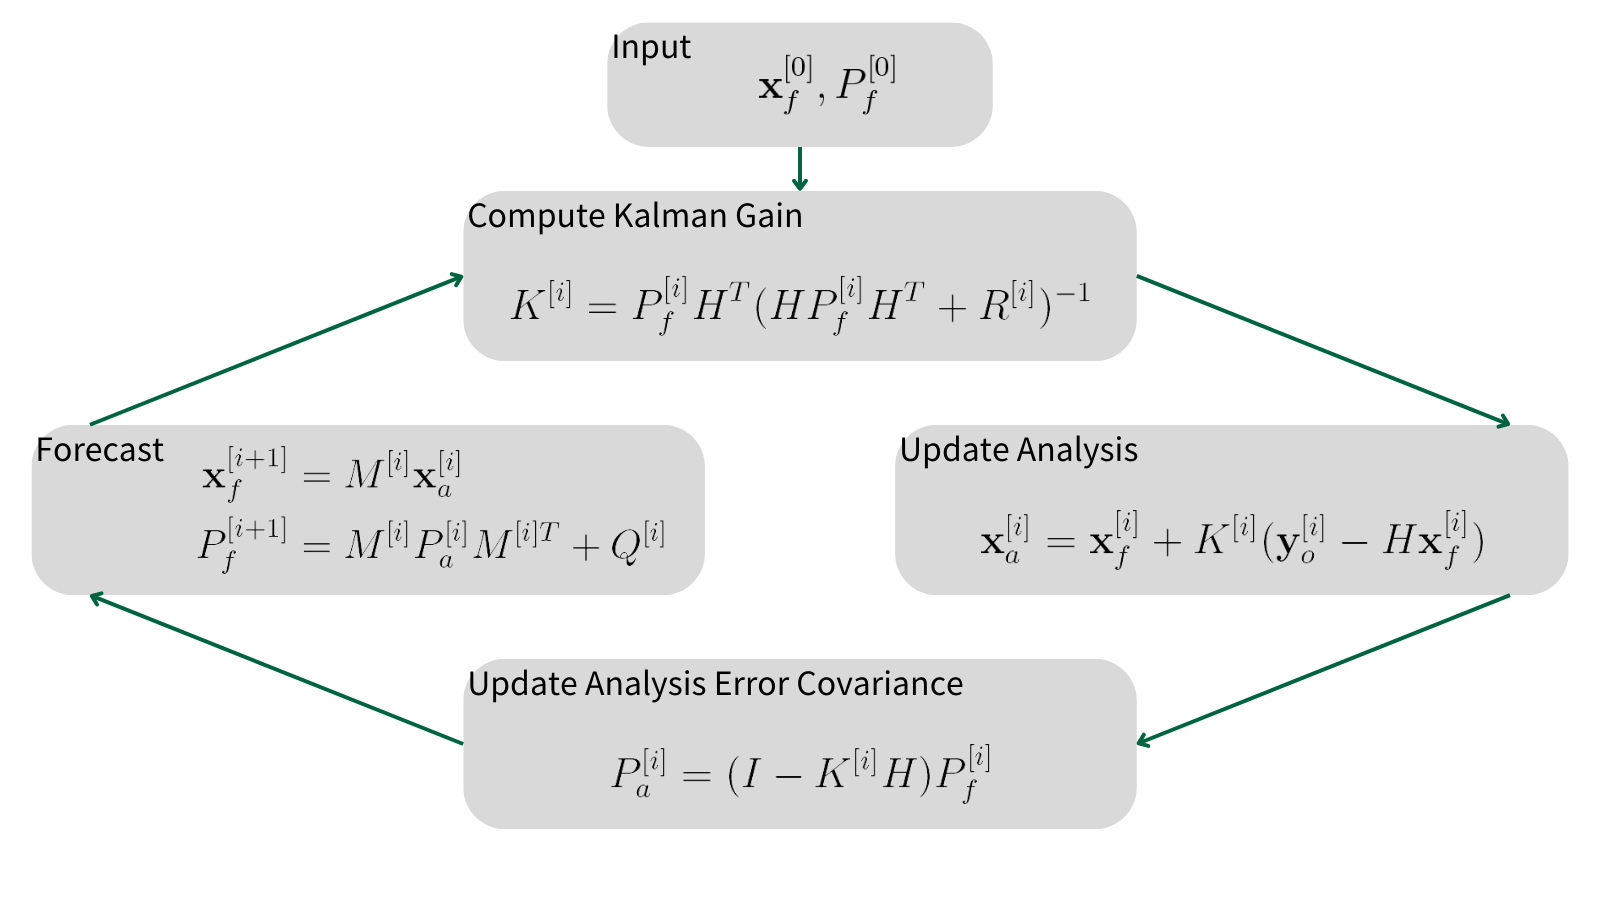
\includegraphics[width=0.99\linewidth]{graphics/Kalman1.png}
    \caption{The flowchart for the standard Kalman Filter scheme.}
    \label{fig:Kalmansteps}
\end{figure}
\end{landscape}
\begin{landscape}
\begin{figure}
    \centering
    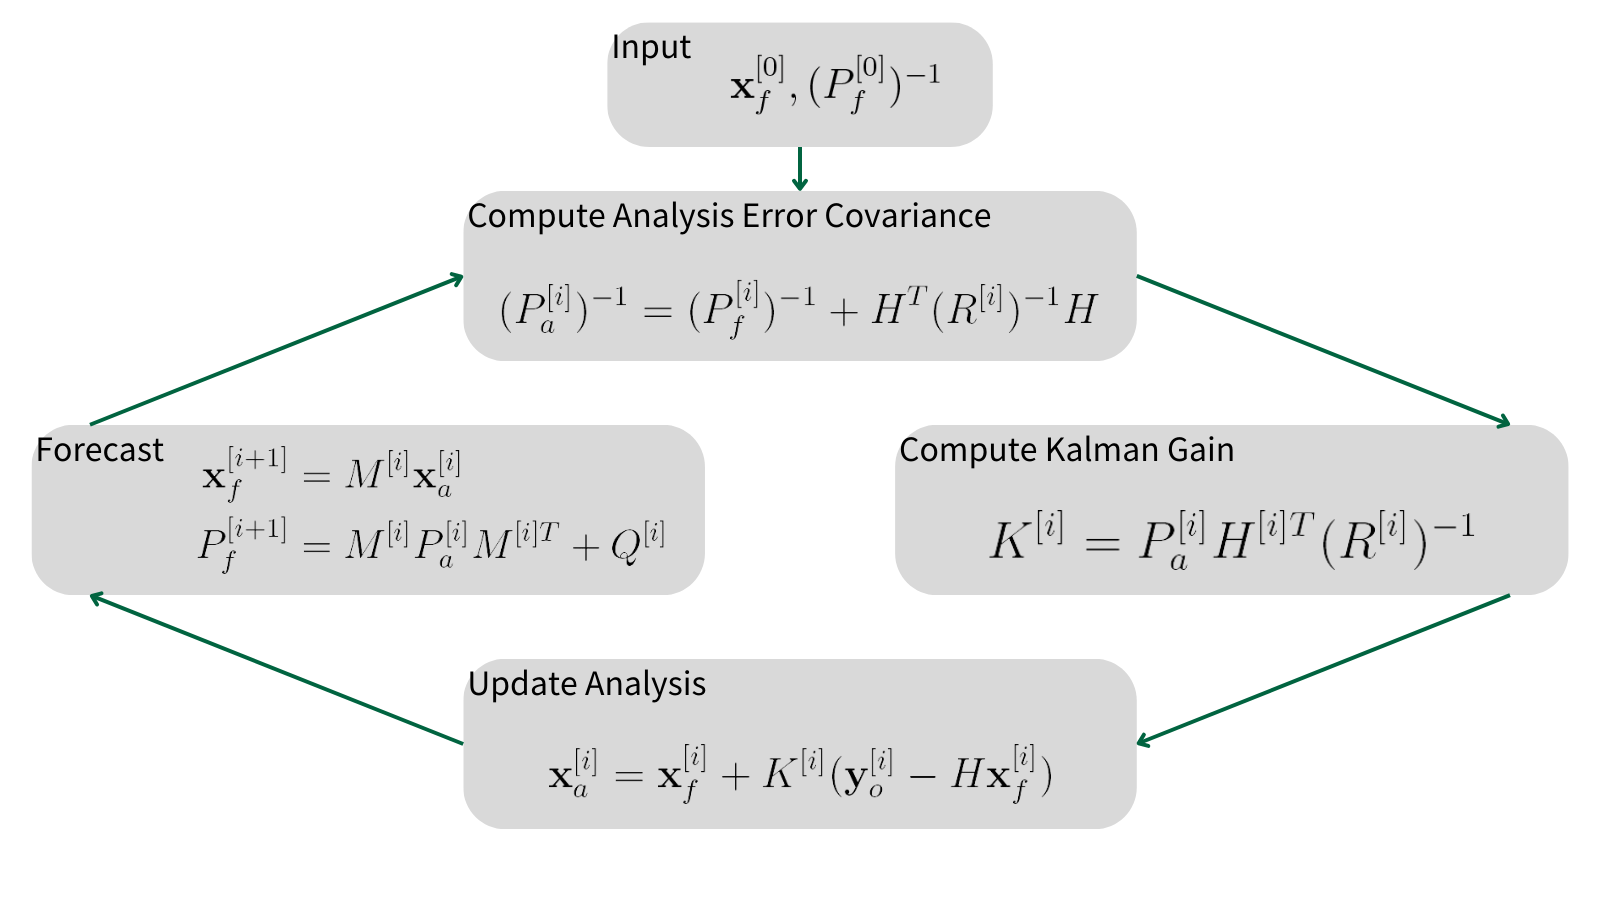
\includegraphics[width=0.99\linewidth]{graphics/Kalman2.png}
    \caption{The flowchart for the alternative Kalman Filter scheme using equivalent expressions for the analysis error covariance and Kalman gain.}
    \label{fig:Kalmansteps2}
\end{figure}
\end{landscape}

\subsection{Python Programming: Demonstration of DA using the Lorenz-63 Model}
\label{subsection:DAsystem}

We will use the Lorenz-63 Model to demonstrate the implementation of Kalman Filter. First, borrow the codes from the last chapter to create a ground truth for the evolution of the Lorenz-63 system.
\begin{lstlisting}
import matplotlib.pyplot as plt
import numpy as np
from scipy.integrate import solve_ivp

def Lorenz63(t, y, sigma=10, beta=8/3, rho=28):
    X, Y, Z = y[0], y[1], y[2]
    dXdt = -sigma*X + sigma*Y
    dYdt = -X*Z + rho*X - Y
    dZdt = X*Y - beta*Z
    return([dXdt, dYdt, dZdt])

t_span = [0,5]
dt = 0.01
x_0 = [-4,10,8]

sol_t = solve_ivp(Lorenz63, t_span, x_0, t_eval=np.arange(t_span[0], t_span[1], dt))
x_t = sol_t.y.T
\end{lstlisting}
From this, we also generate a time-series of synthetic observations by adding Gaussian noises with a constant error covariance of $R = 0.5I$.
\begin{lstlisting}
R = np.diag([0.5]*3)
obs_errors = np.random.multivariate_normal([0,0,0], R, x_t.shape[0])
x_o = x_t + obs_errors    
\end{lstlisting}
Since the Lorenz-63 system is non-linear, for the algorithm of Kalman Filter to work properly, we have to use the \textit{Tangent Linear Model} in place of $M^{[i]}$ when computing $P_f^{[i]}$:
\begin{align}
M^{[i]} = I + (\frac{\partial F}{\partial \textbf{x}})_a^{[i]} \Delta t
\end{align}
where $\partial F/\partial \textbf{x}$ is the Jacobian of the Lorenz-63 system as in (\ref{eqn:lorenzjac}). We will integrate the model forward in time using the simple \textit{Euler method} at the forecast step. On the other hand, at the analysis step, we have to compute the Kalman gain and analysis (as well as its error covariance). To initialize, we will make a guess of \smash{$P_f^{[0]} = 0.5I$}, which is not a problem as the Kalman Filter procedure itself will cycle and tune the error covariance. Finally, we simply have $H = I$ as we will use the synthetic observations of all exact variables. The final program will look like this:
\begin{lstlisting}
sigma, beta, rho = 10, 8/3, 28
P_f_i = np.diag([0.5]*3)
H = np.identity(3)
x_a = np.array([[-5,12,6]]) # Assume some initial error
x_f_i = x_a[0,:]

for ii in np.arange(x_t.shape[0]):

    Ts = ii*dt # Forecast start time
    Ta = (ii+1)*dt # Forecast end time (DA analysis time)

    #--------------
    # Analysis Step
    #--------------

    K_i = P_f_i @ H.T @ np.linalg.inv(H @ P_f_i @ H.T + R) # Compute Kalman gain

    d = x_o[ii, :] - H @ x_f_i # Innovation
    x_a_i = x_f_i + K_i @ d # Update analysis
    P_a_i = (np.identity(3) - K_i @ H) @ P_f_i # plus its error covariance
    
    if ii >= 1:
        x_a = np.vstack([x_a, [x_a_i]]) # Save the analysis output

    #--------------
    # Forecast Step
    #--------------
    
    x_f_i = x_a_i + np.array(Lorenz63(Ts, x_a_i))*dt # Forecast by Euler
    Jcb = np.array([[-sigma,       sigma,    0        ],
                    [rho-x_f_i[2], -1,       -x_f_i[0]],
                    [x_f_i[1],     x_f_i[0], -beta    ]]) # Jacobian
    M_i = np.identity(3) + Jcb*dt # Tangent Linear Model
    P_f_i = M_i @ P_a_i @ M_i.T + np.diag([0.1]*3) # Assume Q = 0.1I
\end{lstlisting}
Let's visualize the performance of our DA system by looking at the errors:
\begin{lstlisting}
err = np.sum(np.sqrt((x_a - x_t)**2), axis=1)

plt.plot(np.arange(t_span[0], t_span[1], dt), err, c="r", label="Error")
plt.hlines(0.5,0,5,linestyles="--",colors="k")
plt.legend()
plt.xlabel("Time")
plt.ylabel("Magnitude")
plt.title("Kalman Filter")
plt.text(4.5,0.55,"0.5",fontsize=16)

plt.savefig("Kalman Filter", dpi=300, bbox_inches="tight")
\end{lstlisting}
\begin{figure}[h!]
    \centering
    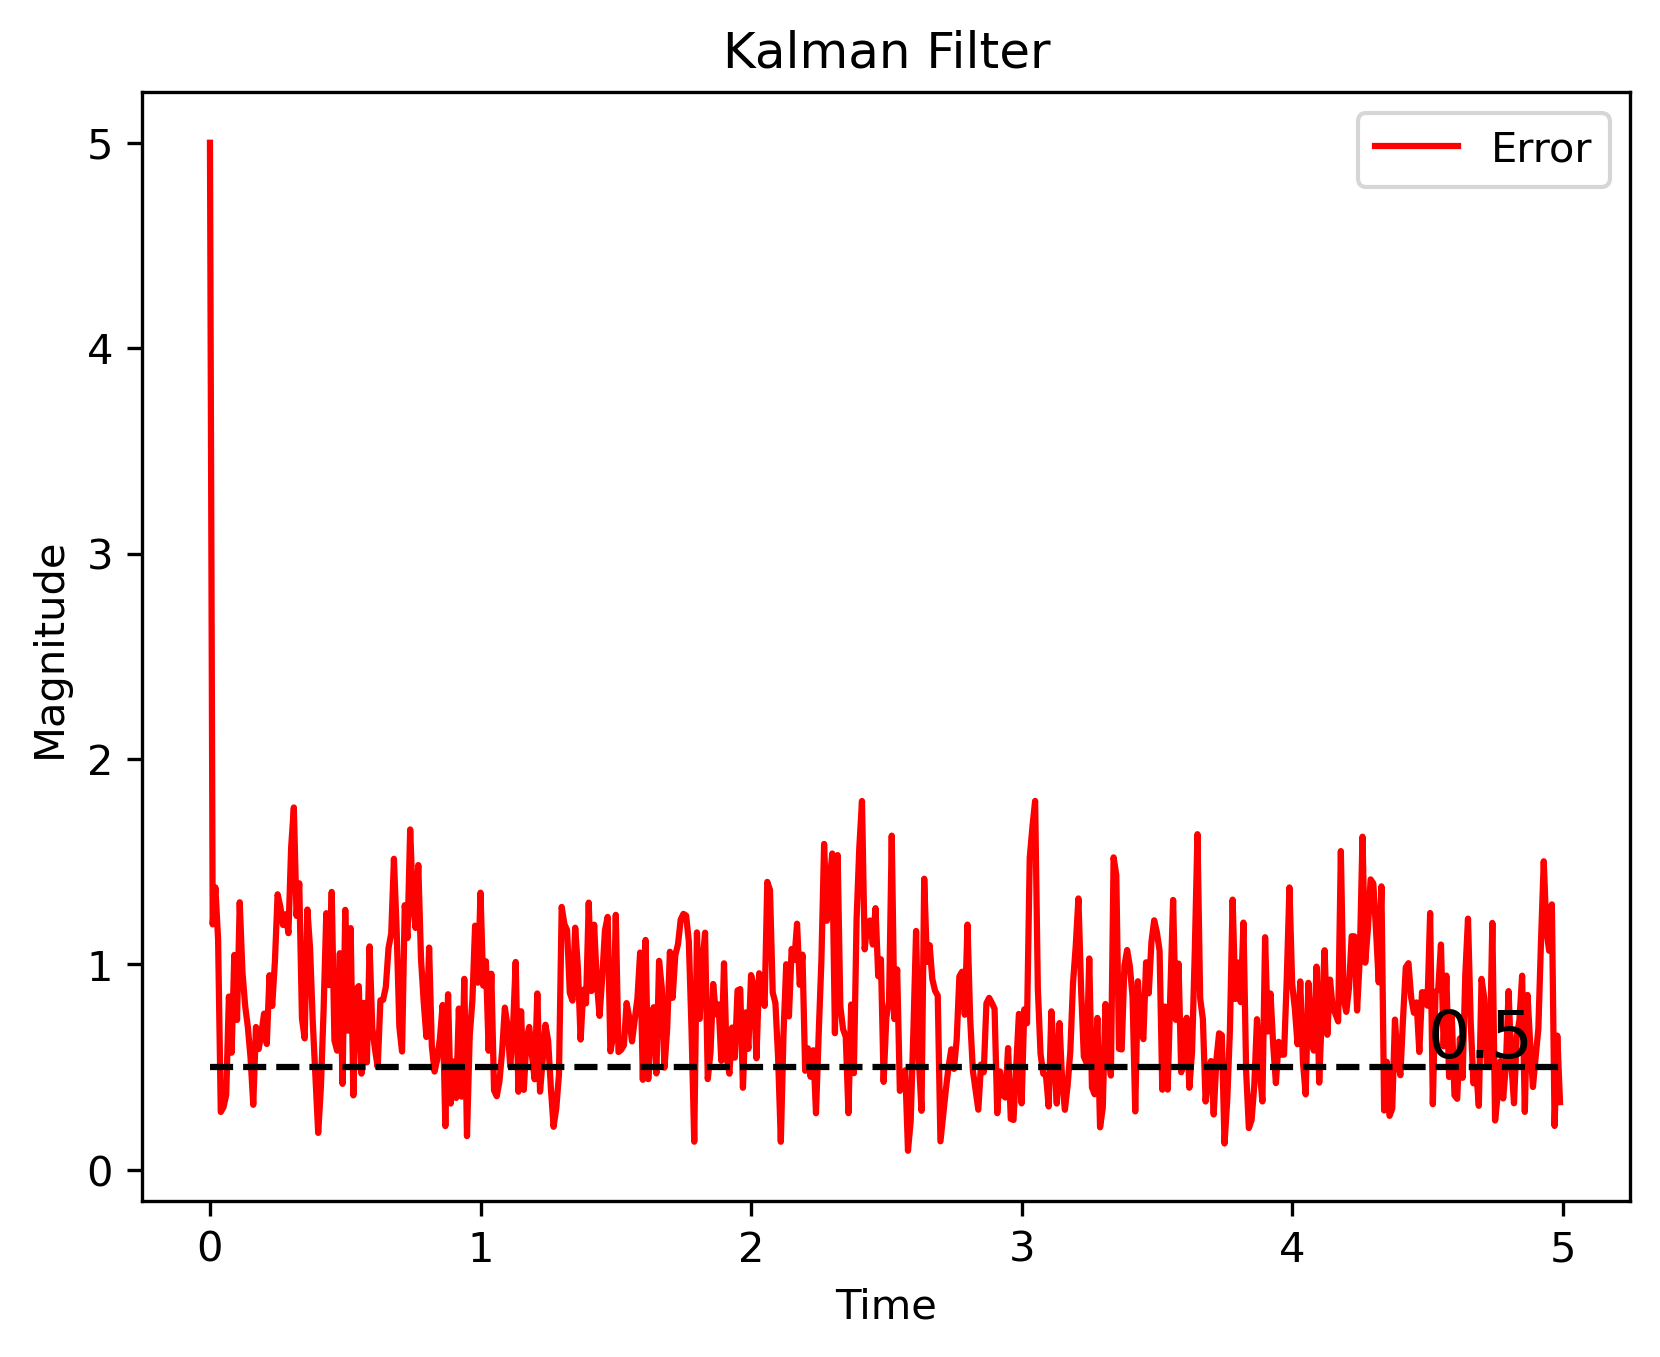
\includegraphics[width=0.75\linewidth]{graphics/Kalman3.png}
    \caption{The evolution of the root-mean-squared error in the Lorenz-63 Model with a Kalman Filter DA system.}
    \label{fig:kalman3}
\end{figure}
From Figure \ref{fig:kalman3}, we can see that the error quickly diminishes at just the beginning of DA and successfully remains at a low level that is slightly above the given observation error.

\section{Exercise}

\begin{Exercise}
Prove the following vector calculus identities using the Index Notation.
\begin{enumerate}[label=(\alph*)]
    \item $\nabla \cdot (\nabla \times \vec{v}) = 0$;
    \item $\nabla \times \nabla u = \textbf{0}$;
    \item $\nabla \times (\nabla \times \vec{v}) = \nabla (\nabla \cdot \vec{v}) - \nabla^2 \vec{v}$
    \item $\nabla \cdot (\vec{u} \times \vec{v}) = \vec{v} \cdot (\nabla \times \vec{u}) - \vec{u} \cdot (\nabla \times \vec{v})$.
\end{enumerate}
\end{Exercise}

\begin{Exercise}
Confirm that if $\vec{u}$ and $\vec{v}$ are two vectors in the tensor sense, then the cross product
\begin{align*}
w_i = \epsilon_{ijk}u_jv_k
\end{align*}
as in (\ref{eqn:crosstens}) must also be the components of a vector via Quotient Law.
\end{Exercise}

\begin{Exercise}
Given a two-dimensional plane stress with two measurements of normal/shear tractions $(7,4)$ and $(9,-3)$ that are assumed to be accurate, find the corresponding Mohr's Circle and the angle between the two oriented surfaces on which the measurements are taken.
\end{Exercise}

\begin{Exercise}
A three-dimensional stress tensor is known to have principal stresses of $\sigma_1, \sigma_2, \sigma_3 = 3,2,-1$. Determine if the following normal/shear traction pairs are possible:
\begin{enumerate}[label=(\alph*)]
    \item $(0,1)$;
    \item $(1.5,1.25)$;
    \item $(4,1)$;
    \item $(2.4,-0.6)$.
\end{enumerate}
\end{Exercise}

\begin{Exercise}
Derive the continuity equation for any extensive quantity, let's say specific humidity $q$:
\begin{align*}
\frac{\partial (\rho q)}{\partial t} + \nabla \cdot(\rho q \textbf{v}) = 0
\end{align*}
if there is no sink or source so that $dq/dt=0$.
\end{Exercise}

\begin{Exercise}
Modify the DA system in Section \ref{subsection:DAsystem} so that it only assimilates selected but not all variables (let's say, $X$ and $Z$), and also try to change the values of $R$ and $Q$.
\end{Exercise}
\chapter*{Answers to Exercises}
\addcontentsline{toc}{chapter}{Answers to Exercises}
\rohead{Answer to Exercises}
\lehead{Answer to Exercises}
\shipoutAnswer
\appendix
\rohead{\headmark}
\lehead{\headmark}

\definecolor{prussianblue}{rgb}{0.0, 0.19, 0.33}

\renewcommand{\chapterformat}{\raggedleft \colorbox{prussianblue}{%
\centering\textit{\textcolor{white}{{\Large Appendix} {\Huge \thechapter}}}}}

\chapter{Supplementary Information for the Main Text}

\section{Chapter \ref*{chapter:invdet}}
\label{section:invdetappend}

\paragraph{Properties \ref*{proper:zerodet}}
Consider an $n \times n$ square matrix $A$ that has two identical and adjacent rows with indices $i_1$ and $i_2$, where $i_2 = i_1 + 1$ (hence one of the indices is odd and another is even), then cofactor expansion along the odd row (let's say $i_1$) will give
\begin{subequations}
\begin{align}
\abs{A} &= \sum_{k=1}^{n} A_{i_1k}C_{i_1k} \nonumber \\
&= \sum_{k=1}^{n} (-1)^{i_1+k}A_{i_1k}\det(M_{i_1k})
\end{align}
by Properties \ref{proper:cofactorex} and Definition \ref{defn:cofactor}. Similarly, by considering the even row, we have
\begin{align}
\abs{A} &= \sum_{k=1}^{n} A_{i_2k}C_{i_2k} \nonumber \\
&= \sum_{k=1}^{n} (-1)^{i_2+k}A_{i_2k}\det(M_{i_2k})
\end{align}
\end{subequations}
But since the $i_1$-th and $i_2$-th row are identical, $A_{i_1k} = A_{i_2k}$. Furthermore, as these two identical rows are also adjacent, the minors $M_{i_1k} = M_{i_2k}$ are also equal. The only difference between the two expressions for $|A|$ above is the $(-1)^{i+j}$ factor. And because $i_1$ is odd and $i_2$ is even, they are differed by a negative sign only. Explicitly, we have
\begin{align}
\abs{A} &= \sum_{k=1}^{n} (-1)^{i_1+k}A_{i_1k}\det(M_{i_1k}) \nonumber \\
&= \sum_{k=1}^{n} (-1)^{(i_2-1)+k}A_{i_2k}\det(M_{i_2k}) \nonumber \\
&= (-1) \sum_{k=1}^{n} (-1)^{i_2+k}A_{i_2k}\det(M_{i_2k}) \nonumber \\
&= -\abs{A}
\end{align}
Therefore $\abs{A} = -\abs{A}$ and $\abs{A} = 0$ must equal to zero. Now we can generalize the results to non-adjacent, proportional rows by doing the first and third kind (multiplication and swapping) of elementary row operations when appropriate with the aid of Properties \ref{proper:elementaryopdet}, and the second case in Properties \ref{proper:zerodet} is completed. Subsequently, for the addition/subtraction type of elementary row operations, let's say $R_{p} + cR_{q} \to R_{p}$ is applied on some matrix $A$ (this $A$ is not the same one as in the first part) to produce $A'$, then
\begin{align*}
A' = 
\begin{bmatrix}
\vdots & \vdots & & \vdots\\
A_{p1} + cA_{q1} & A_{p2} + cA_{q2} & \cdots & A_{pn} + cA_{qn} \\
\vdots & \vdots & & \vdots\\
A_{q1} & A_{q2} & \cdots & A_{qn} \\
\vdots & \vdots & & \vdots
\end{bmatrix}
\end{align*}
where we have only written out the rows $R_p$ and $R_q$. By applying cofactor expansion along $R_p$ following Properties \ref{proper:cofactorex}, we have
\begin{align}
\abs{A'} &= \sum_{k=1}^{n} [(A_{pk} + cA_{qk}) C_{pk}] \nonumber \\
&= \sum_{k=1}^{n} A_{pk}C_{pk} + c\sum_{k=1}^{n} A_{qk}C_{pk}
\end{align}
We identify the first term with $\abs{A}$ that is computed using cofactor expansion on the row $R_p$ of $A$. The second term can be thought of as the determinant of a matrix $\tilde{A}$ that is formed by replacing the $p$-th row $R_p$ by the $q$-th row $R_q$ in $A$ and subsequently expanded along that row. So $\tilde{A}$ practically has two identical rows $R_p = R_q$ and by the previous result the value of $\abs{\tilde{A}}$ is zero. Therefore
\begin{align}
\abs{A'} = \abs{A} + c\abs{\tilde{A}} = \abs{A} + c(0) = \abs{A}    
\end{align} implying that the addition/subtraction type of elementary row operations does not affect the value of the determinant.

\section{Chapter \ref*{chap:vec_space}}
\label{section:vecspaceappend}

\paragraph{Properties \ref*{proper:subspace_n_span}}  

$\mathcal{W}$ as a subspace of $\mathbb{R}^n$ contains at most $n$ linearly independent vectors. Assume $\mathcal{W}$ is non-empty and take any non-zero vector in $\mathcal{W}$, denote it by $\vec{v}^{(1)}$. The span of $\mathcal{\beta} = \{\vec{v}^{(1)}\}$ is itself a subspace $\mathcal{B} = \text{span}(\mathcal{\beta})$ of the subspace $\mathcal{W}$ by noting that it is a subset of $\mathcal{W}$ and using the first part of Properties \ref{proper:subspace_n_span}. If this subspace $\mathcal{B}$ of the subspace $\mathcal{W}$ is exactly $\mathcal{W}$, in the sense that no other $\vec{v} \in \mathcal{W}$ is not included by $\mathcal{B} = \text{span}(\mathcal{\beta})$, then we are done because this subspace is a span by construction. Otherwise, take another non-zero vector $\vec{v}^{(2)} \in \mathcal{W}$ which is linearly independent of $\vec{v}^{(1)}$ and add it to $\mathcal{\beta}$. Now $\mathcal{B} = \text{span}(\mathcal{\beta}) = \text{span}(\{\vec{v}^{(1)}, \vec{v}^{(2)}\})$ is enlarged by one dimension but still a subspace of $\mathcal{W}$ and we can check if it coincides with $\mathcal{W}$, otherwise, repeat the procedure with $\vec{v}^{(3)}, \vec{v}^{(4)}, \ldots$ until $\text{span}(\mathcal{S}) = \mathcal{W}$ then we can stop. Remember we can at most add up to $\vec{v}^{(n)}$ since $\mathcal{W}$ contains at most $n$ linearly independent vectors, so in the middle of somewhere we would done with $\vec{v}^{(p)}$, where $p \leq n$, and hence we know that $\mathcal{W}$ is some span (and a $p$-dimensional subspace).

\paragraph{Dependence relations}

We will show this for the case of row addition/subtraction only because the other two types of elementary row operations are easy to check. Without loss of generality, take a dependence relation in the form of $\vec{v}^{(r+1)} = c_1\vec{v}^{(1)} + c_2\vec{v}^{(2)} + \cdots + c_r\vec{v}^{(r)}$ where $A=[\vec{v}^{(1)}|\vec{v}^{(2)}|\cdots|\vec{v}^{(r)}|\vec{v}^{(r+1)}]$, i.e. \begin{align*}
\begin{bmatrix}
\vdots \\
\vec{v}_p^{(r+1)} \\
\vdots \\
\vec{v}_q^{(r+1)} \\
\vdots
\end{bmatrix}
= c_1
\begin{bmatrix}
\vdots \\
\vec{v}_p^{(1)} \\
\vdots \\
\vec{v}_q^{(1)} \\
\vdots
\end{bmatrix}
+ c_2
\begin{bmatrix}
\vdots \\
\vec{v}_p^{(2)} \\
\vdots \\
\vec{v}_q^{(2)} \\
\vdots
\end{bmatrix} + \cdots + 
c_r
\begin{bmatrix}
\vdots \\
\vec{v}_p^{(r)} \\
\vdots \\
\vec{v}_q^{(r)} \\
\vdots
\end{bmatrix}
\end{align*}
The elementary row operation of adding $c_q$ times row $R_q$ to row $R_p$ then produces a new matrix $A'$ with column vectors
\begin{align*}
\vec{v}^{(j)'}
=
\begin{bmatrix}
\vdots \\
\vec{v}_p^{(j)} + c_q\vec{v}_q^{(j)} \\
\vdots \\
\vec{v}_q^{(j)} \\
\vdots
\end{bmatrix}
\end{align*}
for all $j$. Therefore,
\begin{align*}
\vec{v}^{(r+1)'} &= \begin{bmatrix}
\vdots \\
\vec{v}_p^{(r+1)} + c_q\vec{v}_q^{(r+1)} \\
\vdots \\
\vec{v}_q^{(r+1)} \\
\vdots
\end{bmatrix} \\
&=
\begin{bmatrix}
\vdots \\
(c_1\vec{v}_p^{(1)} + c_2\vec{v}_p^{(2)} + \cdots + c_r\vec{v}_p^{(r)}) + c_q(c_1\vec{v}_q^{(1)} + c_2\vec{v}_q^{(2)} + \cdots + c_r\vec{v}_q^{(r)}) \\
\vdots \\
(c_1\vec{v}_q^{(1)} + c_2\vec{v}_q^{(2)} + \cdots + c_r\vec{v}_q^{(r)}) \\
\vdots
\end{bmatrix}  
\end{align*}
by the original dependence relation, which is then equal to
\begin{align*}
&\quad \begin{bmatrix}
\vdots \\
c_1(\vec{v}_p^{(1)} + c_q\vec{v}_q^{(1)}) \\
\vdots \\
c_1\vec{v}_q^{(1)} \\
\vdots
\end{bmatrix}
+
\begin{bmatrix}
\vdots \\
c_2(\vec{v}_p^{(2)} + c_q\vec{v}_q^{(2)}) \\
\vdots \\
c_2\vec{v}_q^{(2)} \\
\vdots
\end{bmatrix} 
+ \cdots +
\begin{bmatrix}
\vdots \\
c_r(\vec{v}_p^{(r)} + c_q\vec{v}_q^{(r)}) \\
\vdots \\
c_r\vec{v}_q^{(r)} \\
\vdots
\end{bmatrix} \\
&= c_1\vec{v}^{(1)'} + c_2\vec{v}^{(2)'} + \cdots + c_r\vec{v}^{(r)'}
\end{align*}
This shows that the same dependence relation holds between the new column vectors $\vec{v}^{(j)'}$, $j = 1,2,\ldots,r+1$.

\paragraph{Steinitz Replacement Theorem}

\begin{thm}[Steinitz Replacement Theorem]
\label{thm:Steinitz}
%G = \gamma
%S = \eta
%H = \gamma'
Given a vector space $\mathcal{V}$ generated by a set $\mathcal{\gamma}$ consisting of $n$ vectors (not necessarily linearly independent), and another set $\mathcal{\eta}$ containing $m$ linearly independent vectors from $\mathcal{V}$. Then $m \leq n$ and there exists a subset $\mathcal{\gamma'}$ of $\mathcal{\gamma}$ with exactly $n-m$ vectors such that $\mathcal{\eta} \cup \mathcal{\gamma'}$ spans $\mathcal{V}$.
\end{thm}
\begin{proof}
We proceed with mathematical induction on $m$. The base case $m = 0$ is trivial as $\mathcal{\eta} = \varnothing$ and $\mathcal{\gamma'} = \mathcal{\gamma}$. Now assume that the statement is true for some integer $m = k \geq 0$ and we have to prove it for $m = k+1$. Let $\mathcal{\eta} = \{\vec{v}^{(1)}, \vec{v}^{(2)}, \ldots, \vec{v}^{(k)}, \vec{v}^{(k+1)}\}$ be a subset of $\mathcal{V}$ with $m = k+1$ linearly independent vectors. It is apparent that after removing $\vec{v}^{(k+1)}$ from $\mathcal{\eta}$, $\{\vec{v}^{(1)}, \vec{v}^{(2)}, \ldots, \vec{v}^{(k)}\}$ is still linearly independent. Then we can use the induction hypothesis to obtain $k \leq n$ and a subset $\{\vec{u}^{(1)}, \vec{u}^{(2)}, \ldots, \vec{u}^{(n-k)}\}$ of $\mathcal{\gamma}$ so that $\{\vec{v}^{(1)}, \vec{v}^{(2)}, \ldots, \vec{v}^{(k)}\} \cup \{\vec{u}^{(1)}, \vec{u}^{(2)}, \ldots, \vec{u}^{(n-k)}\}$ generates $\mathcal{V}$. So $\vec{v}^{(k+1)} \in \mathcal{V}$ can be written as the linear combination of
\begin{align*}
\vec{v}^{(k+1)} = a_1\vec{v}^{(1)} + a_2\vec{v}^{(2)} + \cdots + a_k\vec{v}^{(k)} + b_1\vec{u}^{(1)} + b_2\vec{u}^{(2)} + \cdots + b_{n-k}\vec{u}^{(n-k)} 
\end{align*}
It must be true that $n - k \geq 1$, so that some $b_j$ are present for otherwise $\vec{v}^{(k+1)}$ will be reduced to a linear combination of $\vec{v}^{(j)}$ and contradicts the assumption that $\mathcal{\eta}$ is linearly independent. Hence $m = k + 1 \leq n$. By part (b) of Theorem \ref{thm:plusminus}, $\text{span}(\mathcal{\eta} \cup \{\vec{u}^{(1)}, \vec{u}^{(2)}, \ldots, \vec{u}^{(n-k)}\}) = \text{span}(\{\vec{v}^{(1)}, \vec{v}^{(2)}, \ldots, \vec{v}^{(k)}, \vec{v}^{(k+1)}\} \cup \{\vec{u}^{(1)}, \vec{u}^{(2)}, \ldots, \vec{u}^{(n-k)}\}) = \text{span}(\{\vec{v}^{(1)}, \vec{v}^{(2)}, \ldots, \vec{v}^{(k)}\} \cup \{\vec{u}^{(1)}, \vec{u}^{(2)}, \ldots, \vec{u}^{(n-k)}\}) \\ = \mathcal{V}$ (the last equality follows from the induction hypothesis). For the same reason, in particular, some $b_j$ has to be non-zero, let's say $b_1$. Therefore we can write
\begin{align*}
\vec{u}_1 = -\frac{a_1}{b_1}\vec{v}^{(1)} -\frac{a_2}{b_1}\vec{v}^{(2)} - \cdots - \frac{a_k}{b_1}\vec{v}^{(k)} + \frac{1}{b_1}\vec{v}^{(k+1)} - \frac{b_2}{b_1}\vec{u}^{(2)} - \cdots - \frac{b_{n-k}}{b_1}\vec{u}^{(n-k)}
\end{align*}
as a linear combination of $\vec{v}^{(1)}, \vec{v}^{(2)}, \ldots, \vec{v}^{(k)}, \vec{v}^{(k+1)}$ and $\vec{u}^{(2)}, \ldots, \vec{u}^{(n-k)}$. Let $\mathcal{H} = \{\vec{u}^{(2)}, \ldots, \vec{u}^{(n-k)}\}$. Again by part (b) of Theorem \ref{thm:plusminus}
\begin{align*}
&\quad \text{span}(\mathcal{\eta} \cup \{\vec{u}^{(1)}, \vec{u}^{(2)}, \ldots, \vec{u}^{(n-k)}\}) \\
&= \text{span}(\{\vec{v}^{(1)}, \vec{v}^{(2)}, \ldots, \vec{v}^{(k)}, \vec{v}^{(k+1)}\} \cup \{\vec{u}^{(1)}, \vec{u}^{(2)}, \ldots, \vec{u}^{(n-k)}\}) \\
&= \text{span}(\{\vec{v}^{(1)}, \vec{v}^{(2)}, \ldots, \vec{v}^{(k)}, \vec{v}^{(k+1)}\} \cup \{\vec{u}^{(2)}, \ldots, \vec{u}^{(n=-k)}\}) \\
&= \text{span}(\mathcal{\eta} \cup \mathcal{\gamma'})
\end{align*}
But we just have $\text{span}(\mathcal{\eta} \cup \{\vec{u}_1, \vec{u}_2, \ldots, \vec{u}_{n-k}\}) = \mathcal{V}$ from above, which readily shows that $\text{span}(\mathcal{\eta} \cup \mathcal{\gamma'}) = \mathcal{V}$. As $\mathcal{\gamma'}$ is a subset of $\mathcal{\gamma}$ with $n - k-1 = n - (k+1)$ vectors, the theorem is true for $m = k+1$, and the induction is completed.
\end{proof}
The key point of the theorem is that some vectors in a generating set of a vector space can be replaced by the same number of linearly independent vectors from that vector space, hence comes the name of the replacement theorem.

\section{Chapter \ref*{chap:DFT}}
\label{section:DFTappend}

\paragraph{Bessel's Inequality}
By part (d) of Theorem \ref{thm:spectralinner}, we can expand a function $f$ as
\begin{align}
f = \lim_{p \to \infty} \sum_{j=1}^{p} \langle f, \varphi^{(j)} \rangle \varphi^{(j)} 
\end{align}
where $\varphi^{(j)}$ are the orthonormal basis vectors/functions and the partial sum $S_p[f]$ will be just $\sum_{j=1}^{p} \langle f, \varphi^{(j)} \rangle \varphi^{(j)}$. Particularly, the completeness of the orthonormal basis in Properties \ref{proper:hilbertorthosys} means that (see the footnote below)\footnote{Otherwise, if $\norm{\smash{f - \sum_{j=1}^{\infty} \langle f, \varphi^{(j)} \rangle \varphi^{(j)}}}^2 > 0$, then consider $\tilde{\varphi} = f - \sum_{j=1}^{\infty} \langle f, \varphi^{(j)} \rangle \varphi^{(j)}$ which is now a non-zero vector. It will be orthogonal to any of the original basis vectors $\varphi^{(j')}$ as 
\begin{align*}
\langle \tilde{\varphi}, \varphi^{(j')} \rangle &= \langle f - \sum_{j=1}^{\infty} \langle f, \varphi^{(j)} \rangle \varphi^{(j)} , \varphi^{(j')} \rangle \\
&= \langle f, \varphi^{(j')} \rangle - \langle \sum_{j=1}^{\infty} \langle f, \varphi^{(j)} \rangle \varphi^{(j)} , \varphi^{(j')} \rangle \\
&= \langle f, \varphi^{(j')} \rangle - (\cdots + (0) +\langle f, \varphi^{(j')} \rangle (1) + (0) + \cdots) \\
& \quad \text{(Orthonormality of the basis: $\langle \varphi^{(j)}, \varphi^{(j')} \rangle = 1$ } \\ 
& \quad \text{only when $j = j'$ and $0$ if $j \neq j'$)} \\
&=\langle f, \varphi^{(j')} \rangle - \langle f, \varphi^{(j')} \rangle = 0
\end{align*}
which violates the premise of completeness as it will become another vector that is linearly independent of all the other basis vectors and can be added to the basis.}
\begin{align}
\norm{f - \sum_{j=1}^{\infty} \langle f, \varphi^{(j)} \rangle \varphi^{(j)}}^2 = 0 \label{eqn:fcomplete}
\end{align}
On the other hand,
\begin{align} 
\norm{f - S_p(f)}^2 &= \norm{f - \sum_{j=1}^{p} \langle f, \varphi^{(j)} \rangle \varphi^{(j)}}^2 \nonumber \\
&= \left\langle f - \sum_{j=1}^{p} \langle f, \varphi^{(j)} \rangle \varphi^{(j)}, f - \sum_{j=1}^{p} \langle f, \varphi^{(j)} \rangle \varphi^{(j)} \right\rangle \nonumber \\
&= \langle f, f \rangle - \left\langle f, \sum_{j=1}^{p} \langle f, \varphi^{(j)} \rangle \varphi^{(j)} \right\rangle - \left\langle \sum_{j=1}^{p} \langle f, \varphi^{(j)} \rangle \varphi^{(j)}, f \right\rangle \nonumber \\
&\quad + \left\langle \sum_{j=1}^{p} \langle f, \varphi^{(j)} \rangle \varphi^{(j)}, \sum_{j=1}^{p} \langle f, \varphi^{(j)} \rangle \varphi^{(j)} \right\rangle \nonumber \\
&= \norm{f}^2 - \left\langle f, \sum_{j=1}^{p} \langle f, \varphi^{(j)} \rangle \varphi^{(j)} \right\rangle \nonumber \\
&\quad - \overline{\left\langle f, \sum_{j=1}^{p} \langle f, \varphi^{(j)} \rangle \varphi^{(j)} \right\rangle} \quad \text{((1) of Definition \ref{defn:innerprod})} \nonumber \\
&\quad + \sum_{j=1}^{p} \abs{\langle f, \varphi^{(j)} \rangle}^2 \quad \text{(Orthonormality of the basis)} \nonumber \\
&= \norm{f}^2 - 2\Re{\langle f, \sum_{j=1}^{p} \langle f, \varphi^{(j)} \rangle \varphi^{(j)} \rangle} + \sum_{j=1}^{p} \abs{\langle f, \varphi^{(j)} \rangle}^2 \nonumber \\
&= \norm{f}^2 - 2\Re{\sum_{j=1}^{p} (\overline{\langle f, \varphi^{(j)} \rangle} \langle f, \varphi^{(j)} \rangle)} \nonumber \\
& \quad \text{((4) of Properties \ref{proper:innerprod2})}\nonumber \\
&\quad + \sum_{j=1}^{p} \abs{\langle f, \varphi^{(j)} \rangle}^2 \nonumber \\
&= \norm{f}^2 - 2\sum_{j=1}^{p} \abs{\langle f, \varphi^{(j)} \rangle}^2 + \sum_{j=1}^{p} \abs{\langle f, \varphi^{(j)} \rangle}^2 \nonumber \\
&= \norm{f}^2 - \sum_{j=1}^{p} \abs{\langle f, \varphi^{(j)} \rangle}^2
\end{align}
and since $\norm{f - S_p(f)}^2 \geq 0$ is always non-negative, we have the \textit{Bessel's Inequality} as
\begin{align}
\sum_{j=1}^{p} \abs{\langle f, \varphi^{(j)} \rangle}^2 \leq \norm{f}^2  \label{eqn:Bessel}
\end{align}
From Exercise \ref{ex:triangular2}, we can apply the Triangle Inequality to get
\begin{align}
&\quad \norm{(f - \sum_{j=1}^{\infty} \langle f, \varphi^{(j)} \rangle \varphi^{(j)}) + (\sum_{j=1}^{\infty} \langle f, \varphi^{(j)} \rangle \varphi^{(j)} - S_p[f])}^2 \nonumber \\
&= \norm{f - S_p[f]}^2 \leq \norm{f - \sum_{j=1}^{\infty} \langle f, \varphi^{(j)} \rangle \varphi^{(j)}}^2 + \norm{\sum_{j=1}^{\infty} \langle f, \varphi^{(j)} \rangle \varphi^{(j)} - S_p[f]}^2
\end{align}
By Equation (\ref{eqn:fcomplete}), the first term on R.H.S. of the equality is zero. And the second term
\begin{align}
&\quad \norm{\sum_{j=1}^{\infty} \langle f, \varphi^{(j)} \rangle \varphi^{(j)} - S_p[f]}^2 \nonumber \\
&= \norm{\sum_{j=p+1}^{\infty} \langle f, \varphi^{(j)} \rangle \varphi^{(j)}}^2 = \sum_{j=p+1}^{\infty} \abs{\langle f, \varphi^{(j)} \rangle}^2
\end{align}
is a remainder term and when $p \to \infty$, must tend to zero, because $\sum_{j=1}^{p} \abs{\langle f, \varphi^{(j)} \rangle}^2$ is a convergent sequence, seen by applying the \textit{Monotone Convergence Theorem} from elementary Analysis on Bessel's Inequality (\ref{eqn:Bessel}). Therefore, the L.H.S.
\begin{align}
\lim_{p \to \infty}\norm{f - S_p[f]}^2 = 0
\end{align}
also tends to zero as we take the same limit, which implies the $L^2$ convergence for a complete orthonormal basis.

\section{Chapter \ref*{chapter:Markov}}
\label{section:Markovappend}

\paragraph{Properties \ref*{proper:positivestoceig}}

\textit{Reference Materials: \cite{markov}}

Let $\vec{q}$ be any eigenvector of $A^T$ that has an eigenvalue of modulus $\abs{\lambda} = 1$. Then $A^T\vec{q} = \lambda \vec{q}$ by the definition of an eigenvalue-eigenvector problem, i.e.\
\begin{align}
\sum_{k=1}^{n} a_{ki}\vec{q}_k = \lambda \vec{q}_i
\end{align}
where $a_{ji}$ is the $(j,i)$ [$(i,j)$] entry of the matrix $A$ [$A^T$]. Then
\begin{align}
\abs{\lambda \vec{q}_i} = \abs{\lambda}\abs{\vec{q}_i} &= \abs{\sum_{k=1}^{n} a_{ki}\vec{q}_k} \nonumber \\
\abs{\vec{q}_i} &\leq \sum_{k=1}^{n} \abs{a_{ki}}\abs{\vec{q}_k} = \sum_{k=1}^{n} a_{ki}\abs{\vec{q}_k} \quad (\abs{\lambda} = 1)\\
&\text{(Triangle Inequality for complex numbers and $a_{ij}$ are real)} \nonumber
\end{align}
Now assume that for some fixed $i$, $\abs{\vec{q}_i} \geq \abs{\vec{q}_k}$ for $1 \leq k \leq n$. Then the inequality above becomes
\begin{align}
\abs{\vec{q}_i} \leq \sum_{k=1}^{n} a_{ki}\abs{\vec{q}_k} &\leq \sum_{k=1}^{n} a_{ki}\abs{\vec{q}_i} = \abs{\vec{q}_i}  & \text{($\sum_{k=1}^{n} a_{ki}$ sums to $1$)}
\end{align}
By squeezing using $\abs{\vec{q}_i}$ at the both ends, the part $\sum_{k=1}^{n} a_{ki}\abs{\vec{q}_k} \leq \sum_{k=1}^{n} a_{ki}\abs{\vec{q}_i}$ forces that $\abs{\vec{q}_k} = \abs{\vec{q}_i}$ for all $k$ and it also holds for any $i$. This is where the positiveness of $A$ is needed, otherwise $a_{ki}$ can be $0$ and the squeeze becomes vacuous ($0\abs{\vec{q}_k} = 0\abs{\vec{q}_i} = 0$). Moreover, as $\abs{\vec{q}_i} = \abs{\sum_{k=1}^{n} a_{ki}\vec{q}_k}$, incorporating it into the inequality
\begin{align}
\abs{\vec{q}_i} = \abs{\sum_{k=1}^{n} a_{ki}\vec{q}_k} \leq \sum_{k=1}^{n} a_{ki}\abs{\vec{q}_k} &\leq \sum_{k=1}^{n} a_{ki}\abs{\vec{q}_i} = \abs{\vec{q}_i}
\end{align}
and apply squeezing again, the part of Triangle Inequality $\abs{\sum_{k=1}^{n} a_{ki}\vec{q}_k} \leq \sum_{k=1}^{n} a_{ki}\abs{\vec{q}_k}$ becomes an equality $\abs{\sum_{k=1}^{n} a_{ki}\vec{q}_k} = \sum_{k=1}^{n} a_{ki}\abs{\vec{q}_k}$, which means that all the components $\vec{q}_k$ have to lie along the same direction in the complex plane.\footnote{For any two complex number $z_1$ and $z_2$, if $\abs{z_1 + z_2} = \abs{z_1} + \abs{z_2}$, then
\begin{align*}
\abs{z_1 + z_2}^2 &= (z_1 + z_2) \overline{(z_1 + z_2)} \\
&= z_1 \overline{z_1} + z_1 \overline{z_2} + z_2 \overline{z_1} + z_2 \overline{z_2} \\
&= \abs{z_1}^2 + z_1 \overline{z_2} + z_2 \overline{z_1} + \abs{z_2}^2
\end{align*}
but also
$(\abs{z_1} + \abs{z_2})^2 = \abs{z_1}^2 + 2\abs{z_1}\abs{z_2} + \abs{z_2}^2$. Hence we have
\begin{align*}
z_1 \overline{z_2} + z_2 \overline{z_1} = 2\abs{z_1}\abs{z_2}
\end{align*}
Assume that $z_1$ and $z_2$ points in some directions so that $z_1 = \abs{z_1}e^{i\theta_1}$ and $z_2 = \abs{z_2}e^{i\theta_2}$, then
\begin{align*}
z_1 \overline{z_2} + z_2 \overline{z_1} &= \abs{z_1}e^{i\theta_1} \abs{z_2}e^{-i\theta_2} + \abs{z_2}e^{i\theta_2} \abs{z_1}e^{-i\theta_1} \\
&= \abs{z_1}\abs{z_2} e^{i(\theta_1-\theta_2)} + \abs{z_1}\abs{z_2} e^{-i(\theta_1-\theta_2)} \\
&= 2 \abs{z_1}\abs{z_2} (\frac{e^{i(\theta_1-\theta_2)} + e^{-i(\theta_1-\theta_2)}}{2}) \\
&= 2 \abs{z_1}\abs{z_2} \cos(\theta_1-\theta_2) & \text{(Properties \ref{proper:sincoscomplex})}
\end{align*}
but this has to equal to $2\abs{z_1}\abs{z_2}$, thus $\cos(\theta_1-\theta_2) = 1$ and the arguments $\theta_1$ and $\theta_2$ will be the same. Now apply this logic repetitively to $\abs{\sum_{k=1}^{n} a_{ki}\vec{q}_k} = \sum_{k=1}^{n} a_{ki}\abs{\vec{q}_k}$.} Therefore, $\vec{q}$ must be be in the form of $c(1,1,1,\ldots,1)^T$ where $c$ will be any complex constant and this shows that over $\mathbb{C}$, the only linearly independent eigenvector for $A^T$ corresponding to $\abs{\lambda} = 1$ will be $(1,1,1,\ldots,1)^T$, matching the derivation in Properties \ref{proper:markoveigen1} where the eigenvalue is exactly $\lambda = 1$ and the geometric multiplicity is hence $1$ as well. Again, by Properties \ref{proper:eigentransinv}, this result will then also hold for the original matrix $A$ (but the form of the eigenvector will be different).

\section{Chapter \ref*{chapter:Tensor}}
\label{section:tensorappend}

\paragraph{Uniqueness of rank-$2$ and $3$ Isotropic Tensors} The uniqueness of the Kronecker delta as the only isotropic rank-$2$ tensor can be shown as follows. By a \SI{90}{\degree} positive rotation about the $3$-axis, we have
\begin{subequations}
\begin{align}
\textbf{e}'_1 &= \textbf{e}_2 \\
\textbf{e}'_2 &= -\textbf{e}_1 \\
\textbf{e}'_3 &= \textbf{e}_3
\end{align}    
\end{subequations}
and according to (\ref{eqn:aij}), the change of coordinates matrix is
\begin{align}
a_{ij} = 
\begin{bmatrix}
\textbf{e}_1 \cdot \textbf{e}'_1 & \textbf{e}_1 \cdot \textbf{e}'_2 & \textbf{e}_1 \cdot \textbf{e}'_3 \\
\textbf{e}_2 \cdot \textbf{e}'_1 & \textbf{e}_2 \cdot \textbf{e}'_2 & \textbf{e}_2 \cdot \textbf{e}'_3 \\
\textbf{e}_3 \cdot \textbf{e}'_1 & \textbf{e}_3 \cdot \textbf{e}'_2 & \textbf{e}_3 \cdot \textbf{e}'_3 
\end{bmatrix} = 
\begin{bmatrix}
0 & -1 & 0 \\
1 & 0 & 0 \\
0 & 0 & 1
\end{bmatrix}
\label{eqn:rotate903ax}
\end{align}
For a general rank-$2$ tensor $F$, by (\ref{eqn:rank2aF}) its transformation will then be
\begin{align}
\begin{bmatrix}
F'_{11} & F'_{12} & F'_{13} \\
F'_{21} & F'_{22} & F'_{23} \\
F'_{31} & F'_{32} & F'_{33}  
\end{bmatrix} &= 
\begin{bmatrix}
0 & 1 & 0 \\
-1 & 0 & 0 \\
0 & 0 & 1
\end{bmatrix}
\begin{bmatrix}
F_{11} & F_{12} & F_{13} \\
F_{21} & F_{22} & F_{23} \\
F_{31} & F_{32} & F_{33}  
\end{bmatrix} 
\begin{bmatrix}
0 & -1 & 0 \\
1 & 0 & 0 \\
0 & 0 & 1
\end{bmatrix} \nonumber \\
&= \begin{bmatrix}
F_{22} & -F_{21} & F_{23} \\
-F_{12} & F_{11} & -F_{13} \\
F_{32} & -F_{31} & F_{33}
\end{bmatrix}
\end{align}
If the tensor is isotropic such that $F'_{ij} = F_{ij}$, then by comparing the entries on both sides, we must have
\begin{subequations}
\begin{align}
F_{11} &= F_{22} \\
F_{13} = F_{23} = -F_{13} \implies F_{13} &= F_{23} = 0 \\
F_{31} = F_{32} = -F_{31} \implies F_{31} &= F_{32} = 0 
\end{align}
\end{subequations}
By the same technique, we can carry out a \SI{90}{\degree} positive rotation about the $2$-axis to obtain
\begin{subequations}
\begin{align}
F_{11} &= F_{33} \\
F_{12} &= F_{32} = 0 \\
F_{21} &= F_{23} = 0 
\end{align}
\end{subequations}
Therefore, $F_{11} = F_{22} = F_{33}$ and $F_{12} = F_{21} = F_{13} = F_{31} = F_{23} = F_{32} = 0$, the diagonal entries have the same value and all off-diagonal entries are zero, and any isotropic rank-$2$ tensor must be in the form of $\lambda \delta_{ij}$, a constant multiple of the Kronecker delta symbol. We can show the same for the rank-$3$ isotropic tensor to be found. First, do a rotation about the $(1,1,1)^T$ axis so that the effect is a subscript permutation $1 \to 2 \to 3 \to 1$, then we have
\begin{subequations}
\begin{align}
T_{111} &= T_{222} = T_{333} \\
T_{112} &= T_{223} = T_{331} \\
T_{122} &= T_{233} = T_{311} \\
T_{212} &= T_{323} = T_{131} \\
T_{211} &= T_{322} = T_{133} \\
T_{121} &= T_{232} = T_{313} \\
T_{221} &= T_{332} = T_{113} \\
T_{123} &= T_{231} = T_{312} \\
T_{132} &= T_{321} = T_{213}
\end{align}
\end{subequations}
Next, apply a \SI{90}{\degree} positive rotation about the $3$-axis as suggested by (\ref{eqn:rotate903ax}) before. After some tedious algebra, we can obtain the following relations:
\begin{subequations}
\begin{align}
T_{111} = -T_{222} &\implies T_{111} = T_{222} = T_{333} = 0 \\
T_{112} = T_{221} \quad \text{and}\quad T_{221} = -T_{112} &\implies T_{112} = T_{221} = 0 \\
T_{122} = T_{211} \quad \text{and}\quad  T_{211} = -T_{122} &\implies T_{122} = T_{211} = 0 \\
T_{121} = T_{212} \quad \text{and}\quad  T_{212} = -T_{121} &\implies T_{121} = T_{212} = 0 \\
T_{123} = -T_{213} &\implies \begin{aligned}
T_{123} &= T_{231} = T_{312}  \\
= -T_{213} &= -T_{321} = -T_{132}    
\end{aligned}
\end{align}
The first four of them show that the rank-$3$ isotropic tensor must take a value of zero when there are repeated subscripts. The last relation implies that it will have an opposite sign when the subscripts belong to an odd/even permutation respectively. This coincides with Definition \ref{defn:epsilon} for the epsilon symbol and thus any isotropic rank-$3$ tensor must be in the form of $\lambda\epsilon_{ijk}$, a constant multiple of the epsilon symbol.
\end{subequations}

\chapter{Cyclic Subspaces and Jordan Normal Forms}

Note that this chapter is basically a rewritten summary of Friedberg's Section 5.4 and Chapter 7. 

\section{From Cyclic Subspaces to Cayley-Hamilton Theorem}
\label{section:B1}

A \index{Cyclic Subspace}\keywordhl{cyclic subspace} of a vector space is generated by repeatedly applying the same linear operator on a fixed initial vector and taking the span of all the resulting vectors.
\begin{defn}[Cyclic Subspace]
Given a vector space $\mathcal{V}$ with a linear operator $T: \mathcal{V} \to \mathcal{V}$ on it, and choose a non-zero vector $\vec{v} \in \mathcal{V}$, then the subspace
\begin{align}
\mathcal{W} = \text{span}(\{\vec{v}, T(\vec{v}), T^2(\vec{v}), \ldots\})
\end{align}
is known as the \textit{$T$-cyclic subspace of $\mathcal{V}$ generated by $\vec{v}$}. 
\end{defn}
It is obviously $T$-invariant (Definition \ref{defn:invariantsub}) because for any vector $\vec{w} \in \mathcal{W}$, if we write $\vec{w} = c_0\vec{v} + c_1T(\vec{v}) + c_2T^2(\vec{v}) + \cdots$ due to the span (Definition \ref{defn:span}, extended to an infinite one if needed), then $T(\vec{w}) = c_0T(\vec{v}) + c_1T^2(\vec{v}) + c_2T^3(\vec{v}) + \cdots \in \mathcal{W}$ lies in the $T$-cyclic subspace too. It is also the smallest $T$-invariant subspace that contains $\vec{v}$: For other $T$-invariant subspaces $\mathcal{W}'$ that also contain $\vec{v}$, by definition they contain $T(\vec{v}), T^2(\vec{v}), \ldots$ as well, and by Properties \ref{proper:WcontainsspanS} they have to completely contain the corresponding $T$-cyclic subspace $\mathcal{W} = \text{span}(\{\vec{v}, T(\vec{v}), T^2\vec{v}, \ldots\})$ too, i.e.\ $\mathcal{W} \subseteq \mathcal{W}'$.\par

To proceed further, we need some more intermediate results. First,
\begin{proper}
\label{proper:B12}
Let $T: \mathcal{V} \to \mathcal{V}$ be a linear operator on a \textit{finite-dimensional} vector space $\mathcal{V}$ and $\mathcal{W}$ be a $T$-invariant subspace of $\mathcal{V}$. Then, the characteristic polynomial (Definition \ref{defn:charactereqn}) of the restriction of $T$ to $\mathcal{W}$, that is, $T|_W$ (Definition \ref{defn:restrictionTW}), divides the characteristic polynomial of $T$.
\end{proper}
We refer the readers to Friedberg for the proof. It means that if the characteristic polynomial of $T|_W$ is $g(t)$ and that of $T$ is $f(t)$, then there exists some other polynomial $q(t)$ such that $f(t) = q(t)g(t)$. Next,
\begin{proper}
\label{proper:B13}
Given $T: \mathcal{V} \to \mathcal{V}$ as a linear operator on a \textit{finite-dimensional} vector space $\mathcal{V}$ and let $\mathcal{W}$ be a $T$-cyclic subspace of $\mathcal{V}$ generated by a non-zero vector $\vec{v} \in \mathcal{V}$. If $\dim(\mathcal{W}) = k$, then
\begin{enumerate}[label=(\alph*)]
    \item $\{\vec{v}, T(\vec{v}), T^2(\vec{v}), \ldots, T^{k-1}(\vec{v})\}$ is a basis for $\mathcal{W}$, and
    \item If $a_0 \vec{v} + a_1 T(\vec{v}) + \cdots + a_{k-1}T^{k-1}(\vec{v}) + T^k(\vec{v}) = \textbf{0}$, then the characteristic polynomial of $T|_W$ is $g(t) = (-1)^k (a_0 + a_1t + \cdots + a_{k-1}t^{k-1} + t^k)$.
\end{enumerate}
\end{proper}
Again, we refer the readers to Friedberg for the proof of part (a) as it is explained in detail there. Meanwhile, to show (b), denote the basis in part (a) as $\mathcal{\beta} = \{\vec{v}, T(\vec{v}), T^2(\vec{v}), \ldots, T^{k-1}(\vec{v})\}$. Then we have $T(T^j(\vec{v})) = T^{j+1}(\vec{v})$ for $0 \leq j < k-1$, and $T(T^{k-1}(\vec{v})) = T^k(\vec{v}) = -a_0 \vec{v} - a_1 T(\vec{v}) - \cdots - a_{k-1}T^{k-1}(\vec{v})$. Subsequently, the linear operator $T|_W$ will have a matrix representation of
\begin{align}
[T|_W]_\beta = 
\begin{bmatrix}
0 & 0 & 0 & \cdots & 0 & -a_0 \\
1 & 0 & 0 & \cdots & 0 & -a_1 \\
0 & 1 & 0 & \cdots & 0 & -a_2 \\
\vdots & \vdots & \vdots & & \vdots & \vdots \\
0 & 0 & 0 & \cdots & 1 & -a_{k-1}
\end{bmatrix}
\end{align}
Its characteristic polynomial (in $t$) is then directly obtained by repeated cofactor expansion (Properties \ref{proper:cofactorex}) along the rows from top to bottom:
\begin{align}
&\quad \det([T|_W]_\beta - t I) \nonumber \\
&= \begin{vmatrix}
-t & 0 & 0 & \cdots & 0 & -a_0 \\
1 & -t & 0 & \cdots & 0 & -a_1 \\
0 & 1 & -t & \cdots & 0 & -a_2 \\
\vdots & \vdots & \vdots & & \vdots & \vdots \\
0 & 0 & 0 & \cdots & 1 & -a_{k-1}-t
\end{vmatrix} \nonumber \\
&=
-t
\begin{vmatrix}
-t & 0 & \cdots & 0 & -a_1 \\
1 & -t & \cdots & 0 & -a_2 \\
\vdots & \vdots  & & \vdots & \vdots \\
0 & 0 & \cdots & 1 & -a_{k-1}-t
\end{vmatrix}
+ (-a_0) (-1)^{k+1}
\begin{vmatrix}
1 & -t & 0 & \cdots & 0 \\
0 & 1 & -t & \cdots & 0 \\
\vdots & \vdots & \vdots & & \vdots \\
0 & 0 & 0 & \cdots & 1 
\end{vmatrix} \nonumber \\
&= -t
\begin{vmatrix}
-t & 0 & \cdots & 0 & -a_1 \\
1 & -t & \cdots & 0 & -a_2 \\
\vdots & \vdots  & & \vdots & \vdots \\
0 & 0 & \cdots & 1 & -a_{k-1}-t
\end{vmatrix}
+ a_0 (-1)^k (1) \nonumber \\
&\quad 
\begin{aligned}
&\text{(The determinant of an upper-triangular block is simply} \\    
&\text{the product of its diagonal entries, which are all $1$ here)}
\end{aligned} \nonumber \\
&= (-t)(-t)
\begin{vmatrix}
-t & \cdots & 0 & -a_2 \\
\vdots & & \vdots & \vdots \\
0 & \cdots & 1 & -a_{k-1}-t
\end{vmatrix} + (-t)(-a_1)(-1)^{(k+1)-1} 
\begin{vmatrix}
1 & -t & \cdots & 0 \\
\vdots & \vdots  & & \vdots \\
0 & 0 & \cdots & 1 
\end{vmatrix} \nonumber \\
&\quad + a_0 (-1)^k \nonumber \\
&= t^2 \begin{vmatrix}
-t & \cdots & 0 & -a_2 \\
\vdots & & \vdots & \vdots \\
0 & \cdots & 1 & -a_{k-1}-t
\end{vmatrix}
+ (a_0 + a_1t)(-1)^k \nonumber \\
& \quad \vdots \nonumber\\
&= (-t)^{k-1}(-a_{k-1}-t) + (a_0 + a_1t + \cdots + a_{k-2}t^{k-2})(-1)^k \nonumber \\
&= (a_0 + a_1t + \cdots + a_{k-2}t^{k-2} + a_{k-1}t^{k-1} + t^k)(-1)^k
\end{align}

The Cayley-Hamilton Theorem then easily follows.
\begin{thm}[Cayley-Hamilton Theorem for Linear Operators]
Let $T: \mathcal{V} \to \mathcal{V}$ be a linear operator on a finite-dimensional vector space $\mathcal{V}$ and $f(t)$ be its characteristic polynomial. Then $f(T) = T_0$ yields the zero transformation.
\end{thm}
\begin{proof}
We have to show that for all $\vec{v} \in \mathcal{V}$, $[f(T)](\vec{v}) = \textbf{0}$. Let $\mathcal{W}$ be the $T$-cyclic subspace generated by $\vec{v}$ and $\dim(\mathcal{W}) = k$. By part (a) of Properties \ref{proper:B13}, $T^k(\vec{v})$ can be written as a linear combination of $\{\vec{v}, T(\vec{v}), T^2(\vec{v}), \ldots, T^{k-1}(\vec{v})\}$, and thus there exist scalars $a_j$ such that $a_0 \vec{v} + a_1 T(\vec{v}) + \cdots + a_{k-1}T^{k-1}(\vec{v}) + T^k(\vec{v}) = \textbf{0}$. By part (b) of Properties \ref{proper:B13}, the characteristic polynomial of $T|_W$ is then $g(t) = (-1)^k(a_0 + a_1t + \cdots + a_{k-1}t^{k-1} + t^k)$. These two statements together imply that
\begin{align*}
[g(T)](\vec{v}) &= (-1)^k(a_0\vec{v} + a_1T(\vec{v}) + \cdots + a_{k-1}T^{k-1}(\vec{v}) + T^k(\vec{v})) \\
&= (-1)^k[a_0I + a_1T + \cdots + a_{k-1}T^{k-1} + T^k](\vec{v}) = \textbf{0}
\end{align*}
By Properties \ref{proper:B12}, $g(t)$ divides the characteristic polynomial $f(t)$ of $T$ so that $f(t) = q(t)g(t)$, and therefore
\begin{align*}
[f(T)](\vec{v}) = [q(T)g(T)](\vec{v}) = [q(T)][g(T)(\vec{v})] = [q(T)](\textbf{0}) = \textbf{0}
\end{align*}
so we are done. The Cayley-Hamilton Theorem \ref{thm:CHthmmat} for matrices is then an immediate corollary of this.
\end{proof}

\section{Jordan Normal Forms}
\label{sec:JNF}

\subsection{Generalized Eigenvectors, Existence of Jordan Normal Forms}

We have seen that the matrix in Example \ref{exmp:dummyjordan}
\begin{align*}
A &=
\begin{bmatrix}
1 & -1 \\
0 & 1
\end{bmatrix}
\end{align*}
has only one eigenvalue $\lambda = 1$ and its geometric multiplicity ($1$) is less than the algebraic multiplicity ($2$): there is only one eigenvector $\vec{v}^{(1)} = (1,0)^T$, so that $A\vec{v}^{(1)} = \lambda\vec{v}^{(1)}$, or equivalently $(A - \lambda I)\vec{v}^{(1)} = \textbf{0}$. Now, let's iterate the procedure and consider $(A - \lambda I)\vec{v}^{(2)} = \vec{v}^{(1)}$, then we have
\begin{align*}
\begin{bmatrix}
1-\lambda & -1 \\
0 & 1-\lambda
\end{bmatrix} 
\vec{v}^{(2)}
=
\begin{bmatrix}
1-1 & -1 \\
0 & 1-1
\end{bmatrix}
\vec{v}^{(2)} 
=
\begin{bmatrix}
0 & -1 \\
0 & 0
\end{bmatrix} 
\vec{v}^{(2)}
=
\begin{bmatrix}
1 \\
0
\end{bmatrix} 
\end{align*}
The solution to $\vec{v}^{(2)}$ is clearly $(0,-1)^T$. $\{\vec{v}^{(1)}, \vec{v}^{(2)}\}$ then forms a basis for $\mathbb{R}^2$ in this case. We have successfully salvaged the problem where an eigenvalue is deficient by finding a \index{Generalized Eigenvector}\keywordhl{generalized eigenvector} $\vec{v}^{(2)}$ that fulfills
\begin{align*}
(A - \lambda I)[(A - \lambda I)\vec{v}^{(2)}] &= (A - \lambda I)\vec{v}^{(1)} \\
(A - \lambda I)^2\vec{v}^{(2)} &= \textbf{0}
\end{align*}
This motivates us to make the following definition.
\begin{defn}
Let $T: \mathcal{V} \to \mathcal{V}$ be a linear operator on a vector space $\mathcal{V}$. A non-zero vector $\vec{v} \in \mathcal{V}$ is known as a generalized eigenvector of $T$ corresponding to an eigenvalue of $\lambda$ if
\begin{align}
(T - \lambda I)^p(\vec{v}) &= \textbf{0}
\end{align}
for some integer $p$.
\end{defn}
Clearly, generalized eigenvectors of $p=1$ are just the ordinary eigenvectors. In parallel, we also have
\begin{defn}
Let $T: \mathcal{V} \to \mathcal{V}$ be a linear operator on a vector space $\mathcal{V}$. The \index{Generalized Eigenspace}\keywordhl{generalized eigenspace} of $T$ corresponding to an eigenvalue of $\lambda$ is denoted by $\mathcal{K}_\lambda$, which is a subspace of $\mathcal{V}$ such that
\begin{align}
\mathcal{K}_\lambda = \{\vec{v} \in \mathcal{V} \mid (T - \lambda I)^p(\vec{v}) &= \textbf{0} \text{ for some integer p.}\}
\end{align}
\end{defn}
It is not hard to show that $\mathcal{K}_\lambda$ is $T$-invariant and contains the ordinary eigenspace $\mathcal{E}_\lambda$. We note two of the most relevant results of generalized eigenvectors/eigenspaces without proof.
\begin{proper}
The generalized eigenvectors/eigenspaces corresponding to two distinct eigenvalues $\lambda \neq \mu$ are linearly independent.
\end{proper}
\begin{proper}
The generalized eigenspace $\mathcal{K}_\lambda$ for the linear operator $T$, corresponding to some fixed eigenvalue $\lambda$ with an algebraic mulplticity of $m$, satisfies the following properties:
\begin{enumerate}
    \item $\mathcal{K}_\lambda = \mathcal{N}((T-\lambda I)^m)$,
    \item $\dim(\mathcal{K}_\lambda) = m$.
\end{enumerate}
\end{proper}
As a result, if $T$ has a characteristic polynomial
\begin{align}
p(\lambda) = (\lambda_1-\lambda)^{m_1}(\lambda_2-\lambda)^{m_2}\cdots(\lambda_k-\lambda)^{m_k} \label{eqn:lambdammm}
\end{align}
then
\begin{align}
\mathcal{V} = \mathcal{K}_{\lambda_1} \oplus \mathcal{K}_{\lambda_2} \oplus \cdots \oplus \mathcal{K}_{\lambda_k} \label{eqn:VKKK}
\end{align} 
On the other hand, extending the above example and definitions of generalized eigenvectors/eigenspaces, we can make a \index{Cycle of Generalized Eigenvectors}\keywordhl{cycle of generalized eigenvectors}.
\begin{defn}
Let $T: \mathcal{V} \to \mathcal{V}$ be a linear operator on a vector space $\mathcal{V}$ and $\vec{v} \in \mathcal{V}$ be a generalized eigenvector of $T$ corresponding to the eigenvalue $\lambda$. If $p$ is the smallest positive integer such that $(T-\lambda I)^p (\vec{v}) = \textbf{0}$, then
\begin{align}
&\quad \{(T-\lambda I)^{p-1}(\vec{v}), (T-\lambda I)^{p-2}(\vec{v}), \ldots, (T-\lambda I)(\vec{v}),\vec{v}\} \label{eqn:B6}\\
&\coloneqq \{\vec{v}^{(1)}, \vec{v}^{(2)}, \ldots, \vec{v}^{(p-1)}, \vec{v}^{(p)}\} \nonumber
\end{align}
is called a \textit{cycle of generalized eigenvectors} of $T$ corresponding to $\lambda$ with a length of $p$. The vectors $\vec{v}^{(1)} \coloneqq (T-\lambda I)^{p-1}(\vec{v})$ and $\vec{v}^{(p)} \coloneqq \vec{v}$ are called the \textit{initial vector} and \textit{end vector} of that cycle respectively.
\end{defn}
The initial vector of any cycle of generalized eigenvectors is then the only eigenvector in that cycle.\par

Now we are going to deduce the form of a \index{Jordan Block}\keywordhl{Jordan block} for a cycle of generalized eigenvectors of some linear operator $T$ corresponding to an eigenvalue of $\lambda$. Consider the linear operator $T-\lambda I$ and the cycle described in (\ref{eqn:B6}). It is not hard to see that (\ref{eqn:B6}) is $(T-\lambda I)$-cyclic (as well as $T$-cyclic) and thus it forms a basis $\gamma$ by part (a) of Properties \ref{proper:B13}. Then the matrix representation of $T-\lambda I$ with respect to $\gamma$ is readily seen to be
\begin{align}
[T-\lambda I]_\gamma = 
\begin{bmatrix}
0 & 1 & 0 & \cdots & 0 \\
0 & 0 & 1 & \cdots & 0 \\
\vdots & \vdots & \vdots & & \vdots \\
0 & 0 & 0 & \cdots & 1 \\
0 & 0 & 0 & \cdots & 0
\end{bmatrix}
\end{align}
and thus the matrix representation of $T$, also with respect to $\gamma$, will be
\begin{align}
[T]_\gamma = 
\begin{bmatrix}
\lambda & 1 & 0 & \cdots & 0 \\
0 & \lambda  & 1 & \cdots & 0 \\
\vdots & \vdots & \vdots & & \vdots \\
0 & 0 & 0 & \cdots & 1 \\
0 & 0 & 0 & \cdots & \lambda 
\end{bmatrix} 
\label{eqn:B8}
\end{align}
This $[T]_\gamma$ is then known as the Jordan block of size $p$ corresponding to $\lambda$, which is "almost diagonal" with $1$ above the main diagonal. Note that it has a characteristic polynomial of $g_\gamma(t) = (\lambda-t)^p$. Moreover, it is not hard to check that $([T-\lambda I]_\gamma)^p = [\textbf{0}] = [T_0]_\gamma$ is the zero transformation and $T-\lambda I$ is known as \index{Nilpotent}\keywordhl{nilpotent} (in the generalized eigenspace $\mathcal{K}_\lambda$). To proceed, we first note some intermediate observations.
\begin{thm}
Given $T$ as a linear operator on a vector space $\mathcal{V}$, if $\gamma_1, \gamma_2, \ldots, \gamma_q$ are cycles of generalized eigenvectors of $T$ corresponding to the same eigenvalue $\lambda$ such that the initial vectors of these $\gamma_j$ are linearly independent, then these $\gamma_j$ will be disjoint and their union $\gamma = \bigcup_{j=1}^{q} \gamma_j$ will also be linearly independent.
\end{thm}
\begin{thm}
\label{thm:B27}
Given $T$ as a linear operator on a \textit{finite-dimensional} vector space $\mathcal{V}$ and $\lambda$ as an eigenvalue of $T$, then the associated generalized eigenspace $\mathcal{K}_\lambda$ has a basis consisting of a union of disjoint cycles of generalized eigenvectors corresponding to $\lambda$.
\end{thm}
These two results are derived in Friedberg and we refer the readers to it for the proof. Using our previous example, the matrix
\begin{align*}
\begin{bmatrix}
1 & -1 \\
0 & 1
\end{bmatrix}    
\end{align*}
has a basis made up of two linearly independent, generalized eigenvectors $\gamma = \{(1,0)^T, (0,-1)^T\}$ for the generalized eigenspace $\mathcal{K}_{\lambda=1}$, and thus we can express the matrix as a Jordan block using this \index{Jordan Canonical Basis}\keywordhl{Jordan canonical basis} following (\ref{eqn:B8}) by a coordinate transformation to the $\gamma$ system (refer to Properties \ref{proper:endomorph}):
\begin{align*}
J &= Q^{-1}AQ \\
\begin{bmatrix}
1 & 1 \\
0 & 1
\end{bmatrix} 
&=
\begin{bmatrix}
1 & 0 \\
0 & -1
\end{bmatrix}^{-1} 
\begin{bmatrix}
1 & -1 \\
0 & 1
\end{bmatrix} 
\begin{bmatrix}
1 & 0 \\
0 & -1
\end{bmatrix}
\end{align*}
The final result is that we can derive the \index{Jordan Normal Form}\keywordhl{Jordan Normal Form} of a matrix/linear operator by composing Jordan blocks as a direct sum.
\begin{thm}
Let $T: \mathcal{V} \to \mathcal{V}$ be a linear operator on a finite-dimensional vector space $\mathcal{V}$ and the characteristic polynomial of $T$ splits over the chosen field ($\mathbb{R}$ or $\mathbb{C}$). Then $T$ can be transformed into its Jordan Normal Form as the direct sum of smaller Jordan blocks. Using the matrix representation $A$, we have
\begin{align}
J = Q^{-1}AQ
\end{align}
where $Q$ consists of the union of Jordan canonical bases for all the Jordan blocks in columns.
\end{thm}
By Theorem \ref{thm:B27}, $\mathcal{K}_{\lambda_i}$ has a basis $\gamma_{\lambda_i} = \bigcup_{j=1}^{q} (\gamma_j)_{\lambda_i}$ formed by smaller cycles to the same eigenvalue $\lambda_i$ and hence $[T|_{\mathcal{K}_{\lambda_i}}]_\gamma = {(J_1)}_{\lambda_i} \oplus {(J_2)}_{\lambda_i} \oplus \cdots {(J_q)}_{\lambda_i} = J_{\lambda_i}$, and by (\ref{eqn:VKKK}), we have
\begin{align}
[T]_\beta = J_{\lambda_1} \oplus J_{\lambda_2} \oplus \cdots \oplus J_{\lambda_k}
\end{align}
as its Jordan Normal Form, where $\beta = \bigcup_{i=1}^{k} \gamma_{\lambda_i}$. The Jordan Normal Form of the last example is simply its only Jordan block:
\begin{align*}
J = \begin{bmatrix}
1 & 1 \\
0 & 1
\end{bmatrix} 
\end{align*}
To conclude, Jordan Normal Forms are the generalization and remedy of diagonalized forms where the constraint is relaxed to accommodate the case of deficient eigenvalues, so that it exists whenever the characteristic polynomial splits. But the price is that there will be some extra "1" above the main diagonal in the Jordan blocks of size $\geq 2$. Conversely, if all the Jordan blocks are of size $1$, then it will coincide with the usual diagonalization. For example,
\begin{align*}
J = 
\begin{bmatrix}
\mathcolor{red}{2} & \mathcolor{red}{1} & 0 & 0 & 0 & 0 & 0 \\
\mathcolor{red}{0} & \mathcolor{red}{2} & 0 & 0 & 0 & 0 & 0 \\
0 & 0 & \mathcolor{blue}{3} & \mathcolor{blue}{1} & \mathcolor{blue}{0} & 0 & 0 \\
0 & 0 & \mathcolor{blue}{0} & \mathcolor{blue}{3} & \mathcolor{blue}{1} & 0 & 0 \\
0 & 0 & \mathcolor{blue}{0} & \mathcolor{blue}{0} & \mathcolor{blue}{3} & 0 & 0 \\
0 & 0 & 0 & 0 & 0 & \mathcolor{Green}{3} & 0 \\
0 & 0 & 0 & 0 & 0 & 0 & \mathcolor{purple}{3}
\end{bmatrix}
\end{align*}
consists of one Jordan block corresponding to $\lambda = 2$ of size $2$ (red), one Jordan block corresponding to $\lambda = 3$ of size $3$ (blue), and two Jordan blocks corresponding to $\lambda = 3$ of size $1$ (green and purple). The positions of blocks can be swapped with each other. However, note that a characteristic polynomial (\ref{eqn:lambdammm}) does not uniquely determine the Jordan Normal Form. In the above example, the characteristic polynomial is $p(\lambda) = (2-\lambda)^2(3-\lambda)^5$. But a different Jordan Normal Form like
\begin{align*}
J' =
\begin{bmatrix}
2 & 0 & 0 & 0 & 0 & 0 & 0 \\
0 & 2 & 0 & 0 & 0 & 0 & 0 \\
0 & 0 & 3 & 1 & 0 & 0 & 0 \\
0 & 0 & 0 & 3 & 1 & 0 & 0 \\
0 & 0 & 0 & 0 & 3 & 1 & 0 \\
0 & 0 & 0 & 0 & 0 & 3 & 0 \\
0 & 0 & 0 & 0 & 0 & 0 & 3
\end{bmatrix}
\end{align*}
also shares the same characteristic polynomial. We note in passing that there is a closely related concept called a \index{Minimal Polynomial}\textit{minimal polynomial}, which the readers can search about if they are interested in exploring the deeper theoretical aspect.

\subsection{Methods to Compute Jordan Normal Forms}

In this subsection, we will investigate the techniques to compute the Jordan Normal Form of any given matrix practically.

\begin{exmp}
Derive the Jordan Normal Form of
\begin{align*}
A = 
\begin{bmatrix}
3&3&-2\\ 
-1&0&1\\ 
0&1&1
\end{bmatrix}
\end{align*}
\end{exmp}
\begin{solution}
We leave it to the readers to check that the characteristic polynomial is $p(\lambda) = (1-\lambda)^2(2-\lambda)$. Hence, both the algebraic and geometric multiplicity of $\lambda = 2$ is $1$, which is easy to deal with. The problem will be $\lambda = 1$ which has an algebraic multiplicity of $2$, and there are two possibilities: if the geometric multiplicity is also $2$, then the situation is the same as the usual diagonalization where we have two ordinary eigenvectors. Otherwise, if the geometric multiplicity is $1$, then we will have a single Jordan block of length $2$. Now consider the system $A-I = \textbf{0}$:
\begin{align*}
\left[\begin{array}{@{\,}wc{10pt}wc{10pt}wc{10pt}|wc{10pt}@{\,}}
2 & 3 & -2 & 0  \\ 
-1 & -1 & 1 & 0\\ 
0 & 1 & 0 & 0
\end{array}\right] 
& \to 
\left[\begin{array}{@{\,}wc{10pt}wc{10pt}wc{10pt}|wc{10pt}@{\,}}
1 & \frac{3}{2} & -1 & 0 \\ 
-1 & -1 & 1 & 0 \\ 
0 & 1 & 0 & 0
\end{array}\right] 
& \frac{1}{2}R_1 \to R_1 \\
& \to 
\left[\begin{array}{@{\,}wc{10pt}wc{10pt}wc{10pt}|wc{10pt}@{\,}}
1 & \frac{3}{2} & -1 & 0 \\ 
0 & \frac{1}{2} & 0 & 0 \\ 
0 & 1 & 0 & 0
\end{array}\right] 
& R_2 + R_1 \to R_2 \\
& \to 
\left[\begin{array}{@{\,}wc{10pt}wc{10pt}wc{10pt}|wc{10pt}@{\,}}
1 & \frac{3}{2} & -1 & 0 \\ 
0 & 1 & 0 & 0 \\ 
0 & 0 & 0 & 0
\end{array}\right]
&
\begin{aligned}
2R_2 \to R_2 \\
R_3 - R_2 \to R_3
\end{aligned}
\end{align*}
The nullity is $1$ and there is only one eigenvector. By letting the third entry be the free variable, it is not hard to see that the eigenvector will be $\vec{v}^{(1)} = (1,0,1)^T$. So there will be only one Jordan block, and due to this, we can obtain the next generalized eigenvector in a relatively simple reverse fashion by solving
\begin{align*}
(A - I)\vec{v}^{(2)} &= \vec{v}^{(1)} \\
\begin{bmatrix}
2 & 3 & -2\\ 
-1 & -1 & 1\\ 
0 & 1 & 0
\end{bmatrix}
\vec{v}^{(2)} &=
\begin{bmatrix}
1 \\
0 \\
1
\end{bmatrix}
\end{align*}
We can pick any particular solution for this, and again, we will leave it to the readers to confirm that $\vec{v}^{(2)} = (-1,1,0)^T$ is a valid choice. Finally, we simply note that the eigenvector for the other eigenvalue $\lambda = 2$ is $(-1,1,1)^T$. Thus, the required Jordan Normal Form is
\begin{align*}
Q^{-1}AQ &= 
\begin{bmatrix}
1 & -1 & -1\\
0 & 1 & 1\\
1 & 0 & 1
\end{bmatrix}^{-1}
\begin{bmatrix}
3&3&-2\\ 
-1&0&1\\ 
0&1&1
\end{bmatrix}
\begin{bmatrix}
1 & -1 & -1\\
0 & 1 & 1\\
1 & 0 & 1
\end{bmatrix} \\
J &=
\begin{bmatrix}
1 & 1 & 0 \\
0 & 1 & 0 \\
0 & 0 & 2
\end{bmatrix}
\end{align*}
\end{solution}

Next, we will tackle a much harder case where there are multiple Jordan blocks corresponding to the same eigenvalue.
\begin{exmp}
Convert the matrix
\begin{align*}
A = \begin{bmatrix}
5&-1&-1&-2&0&-1\\ 
-1&19&9&24&6&17\\ 
-1&3&5&4&2&1\\ 
2&-10&-6&-12&-4&-10\\ 
1&-5&-3&-8&2&-5\\ 
-1&1&1&2&0&5
\end{bmatrix}    
\end{align*}
to its Jordan Normal Form.
\end{exmp}
\begin{solution}
We will leave it to the readers to verify that the characteristic polynomial is $p(\lambda) = (4-\lambda)^6$, so the only eigenvalue is $\lambda = 4$. There can be many possible scenarios: the geometric multiplicity is $6$, so there will be $6$ eigenvectors and $6$ singleton Jordan blocks, which reduces to the usual diagonalization. The other extreme will have a single Jordan block of length $6$. In between these two extremes, we may have $2$ to $5$ Jordan blocks of varying sizes. To begin, we compute the eigenvectors that are also the generalized eigenvectors of order $1$, by solving the system $A-4I = \textbf{0}$:
\begin{align*}
& \left[\begin{array}{@{\,}wc{13pt}wc{13pt}wc{13pt}wc{13pt}wc{13pt}wc{13pt}|wc{13pt}@{\,}}
1 & -1 & -1 & -2 & 0 & -1 & 0\\ 
-1 & 15 & 9 & 24 & 6 & 17 & 0\\ 
-1 & 3 & 1 & 4 & 2 & 1 & 0\\  
2 & -10 & -6 & -16 & -4 & -10 & 0\\  
1 & -5 & -3 & -8 & -2 & -5 & 0\\  
-1 & 1 & 1 & 2 & 0 & 1 & 0
\end{array}\right] \\
\to& \left[\begin{array}{@{\,}wc{13pt}wc{13pt}wc{13pt}wc{13pt}wc{13pt}wc{13pt}|wc{13pt}@{\,}}
1 & -1 & -1 & -2 & 0 & -1 & 0\\ 
0 & 14 & 8 & 22 & 6 & 16 & 0\\ 
0 & 2 & 0 & 2 & 2 & 0 & 0\\  
0 & -8 & -4 & -12 & -4 & -8 & 0\\  
0 & -4 & -2 & -6 & -2 & -4 & 0\\  
0 & 0 & 0 & 0 & 0 & 0 & 0
\end{array}\right] &
\begin{aligned}
R_2 + R_1 \to R_2\\
R_3 + R_1 \to R_3\\
R_4 - 2R_1 \to R_4\\
R_5 - R_1 \to R_5\\
R_6 + R_1 \to R_6
\end{aligned} \\
\to& \left[\begin{array}{@{\,}wc{13pt}wc{13pt}wc{13pt}wc{13pt}wc{13pt}wc{13pt}|wc{13pt}@{\,}}
1 & -1 & -1 & -2 & 0 & -1 & 0\\ 
0 & 1 & 0 & 1 & 1 & 0 & 0\\  
0 & 14 & 8 & 22 & 6 & 16 & 0\\ 
0 & -8 & -4 & -12 & -4 & -8 & 0\\  
0 & -4 & -2 & -6 & -2 & -4 & 0\\  
0 & 0 & 0 & 0 & 0 & 0 & 0
\end{array}\right] &
\begin{aligned}
R_2 \leftrightarrow R_3 \\
\frac{1}{2} R_2 \to R_2
\end{aligned} \\
\to& \left[\begin{array}{@{\,}wc{13pt}wc{13pt}wc{13pt}wc{13pt}wc{13pt}wc{13pt}|wc{13pt}@{\,}}
1 & -1 & -1 & -2 & 0 & -1 & 0\\ 
0 & 1 & 0 & 1 & 1 & 0 & 0\\  
0 & 0 & 8 & 8 & -8 & 16 & 0\\ 
0 & 0 & -4 & -4 & 4 & -8 & 0\\  
0 & 0 & -2 & -2 & 2 & -4 & 0\\  
0 & 0 & 0 & 0 & 0 & 0 & 0
\end{array}\right] &
\begin{aligned}
R_3 - 14R_2 \to R_3 \\
R_4 + 8R_2 \to R_4 \\
R_5 + 4R_2 \to R_5
\end{aligned} \\
\to& \left[\begin{array}{@{\,}wc{13pt}wc{13pt}wc{13pt}wc{13pt}wc{13pt}wc{13pt}|wc{13pt}@{\,}}
1 & -1 & -1 & -2 & 0 & -1 & 0\\ 
0 & 1 & 0 & 1 & 1 & 0 & 0\\  
0 & 0 & 1 & 1 & -1 & 2 & 0\\ 
0 & 0 & 0 & 0 & 0 & 0 & 0\\  
0 & 0 & 0 & 0 & 0 & 0 & 0\\  
0 & 0 & 0 & 0 & 0 & 0 & 0
\end{array}\right] &
\begin{aligned}
\frac{1}{8} R_3 \to R_3 \\
R_4 + 4R_3 \to R_4 \\
R_5 + 2R_3 \to R_5
\end{aligned} \\
\to& \left[\begin{array}{@{\,}wc{13pt}wc{13pt}wc{13pt}wc{13pt}wc{13pt}wc{13pt}|wc{13pt}@{\,}}
1 & 0 & 0 & 0 & 0 & 1 & 0\\ 
0 & 1 & 0 & 1 & 1 & 0 & 0\\  
0 & 0 & 1 & 1 & -1 & 2 & 0\\ 
0 & 0 & 0 & 0 & 0 & 0 & 0\\  
0 & 0 & 0 & 0 & 0 & 0 & 0\\  
0 & 0 & 0 & 0 & 0 & 0 & 0
\end{array}\right] & 
\begin{aligned}
R_1 + R_3 \to R_1 \\
R_1 + R_2 \to R_1
\end{aligned}
\end{align*}
The nullity is $3$. We can assign the last three components as the free variables to obtain three eigenvectors: $(0,-1,-1,1,0,0)^T$, $(0,-1,1,0,1,0)^T$, $(-1,0,-2,0,0,1)^T$ (the readers should do the checking), and there will be three Jordan blocks of unknown lengths. Now here is the trick. We create an augmented system where the left is $A-\lambda I$ and the right consists of the three eigenvectors we just obtained. We will derive its RREF but we can reuse the previous reduction step:
\begin{align*}
& \left[\begin{array}{@{\,}wc{13pt}wc{13pt}wc{13pt}wc{13pt}wc{13pt}wc{13pt}|wc{13pt}wc{13pt}wc{13pt}@{\,}}
1 & -1 & -1 & -2 & 0 & -1 & 0 & 0 & -1\\ 
-1 & 15 & 9 & 24 & 6 & 17 & -1 & -1 & 0 \\ 
-1 & 3 & 1 & 4 & 2 & 1 & -1 & 1 & -2\\  
2 & -10 & -6 & -16 & -4 & -10 & 1 & 0 & 0\\  
1 & -5 & -3 & -8 & -2 & -5 & 0 & 1 & 0 \\  
-1 & 1 & 1 & 2 & 0 & 1 & 0 & 0 & 1
\end{array}\right] \\
\to&
\left[\begin{array}{@{\,}wc{13pt}wc{13pt}wc{13pt}wc{13pt}wc{13pt}wc{13pt}|wc{13pt}wc{13pt}wc{13pt}@{\,}}
1 & -1 & -1 & -2 & 0 & -1 & 0 & 0 & -1\\  
0 & 14 & 8 & 22 & 6 & 16 & -1 & -1 & -1 \\ 
0 & 2 & 0 & 2 & 2 & 0 & -1 & 1 & -3\\  
0 & -8 & -4 & -12 & -4 & -8 & 1 & 0 & 2\\ 
0 & -4 & -2 & -6 & -2 & -4 & 0 & 1 & 1 \\    
0 & 0 & 0 & 0 & 0 & 0 & 0 & 0 & 0
\end{array}\right] & 
\begin{aligned}
R_2 + R_1 \to R_2\\
R_3 + R_1 \to R_3\\
R_4 - 2R_1 \to R_4\\
R_5 - R_1 \to R_5\\
R_6 + R_1 \to R_6
\end{aligned} \\
\to&
\left[\begin{array}{@{\,}wc{13pt}wc{13pt}wc{13pt}wc{13pt}wc{13pt}wc{13pt}|wc{13pt}wc{13pt}wc{13pt}@{\,}}
1 & -1 & -1 & -2 & 0 & -1 & 0 & 0 & -1\\  
0 & 1 & 0 & 1 & 1 & 0 & -\frac{1}{2} & \frac{1}{2} & -\frac{3}{2}\\
0 & 14 & 8 & 22 & 6 & 16 & -1 & -1 & -1 \\ 
0 & -8 & -4 & -12 & -4 & -8 & 1 & 0 & 2\\ 
0 & -4 & -2 & -6 & -2 & -4 & 0 & 1 & 1 \\    
0 & 0 & 0 & 0 & 0 & 0 & 0 & 0 & 0
\end{array}\right] & 
\begin{aligned}
R_2 \leftrightarrow R_3 \\
\frac{1}{2} R_2 \to R_2
\end{aligned} \\
\to&
\left[\begin{array}{@{\,}wc{13pt}wc{13pt}wc{13pt}wc{13pt}wc{13pt}wc{13pt}|wc{13pt}wc{13pt}wc{13pt}@{\,}}
1 & -1 & -1 & -2 & 0 & -1 & 0 & 0 & -1\\  
0 & 1 & 0 & 1 & 1 & 0 & -\frac{1}{2} & \frac{1}{2} & -\frac{3}{2}\\ 
0 & 0 & 8 & 8 & -8 & 16 & 6 & -8 & 20 \\ 
0 & 0 & -4 & -4 & 4 & -8 & -3 & 4 & -10\\   
0 & 0 & -2 & -2 & 2 & -4 & -2 & 3 & -5 \\     
0 & 0 & 0 & 0 & 0 & 0 &  0 & 0 & 0
\end{array}\right] & 
\begin{aligned}
R_3 - 14R_2 \to R_3 \\
R_4 + 8R_2 \to R_4 \\
R_5 + 4R_2 \to R_5
\end{aligned} \\
\to&
\left[\begin{array}{@{\,}wc{13pt}wc{13pt}wc{13pt}wc{13pt}wc{13pt}wc{13pt}|wc{13pt}wc{13pt}wc{13pt}@{\,}}
1 & -1 & -1 & -2 & 0 & -1 & 0 & 0 & -1\\  
0 & 1 & 0 & 1 & 1 & 0 & -\frac{1}{2} & \frac{1}{2} & -\frac{3}{2}\\ 
0 & 0 & 1 & 1 & -1 & 2 & \frac{3}{4} & -1 & \frac{5}{2} \\ 
0 & 0 & 0 & 0 & 0 & 0 & 0 & 0 & 0\\   
0 & 0 & 0 & 0 & 0 & 0 & -\frac{1}{2} & 1 & 0 \\     
0 & 0 & 0 & 0 & 0 & 0 &  0 & 0 & 0
\end{array}\right] & 
\begin{aligned}
\frac{1}{8} R_3 \to R_3 \\
R_4 + 4R_3 \to R_4 \\
R_5 + 2R_3 \to R_5
\end{aligned} \\
\to&
\left[\begin{array}{@{\,}wc{13pt}wc{13pt}wc{13pt}wc{13pt}wc{13pt}wc{13pt}|wc{13pt}wc{13pt}wc{13pt}@{\,}}
1 & 0 & 0 & 0 & 0 & 1 & \frac{1}{4} & -\frac{1}{2} & 0\\  
0 & 1 & 0 & 1 & 1 & 0 & -\frac{1}{2} & \frac{1}{2} & -\frac{3}{2}\\ 
0 & 0 & 1 & 1 & -1 & 2 & \frac{3}{4} & -1 & \frac{5}{2} \\ 
0 & 0 & 0 & 0 & 0 & 0 & 0 & 0 & 0\\   
0 & 0 & 0 & 0 & 0 & 0 & -\frac{1}{2} & 1 & 0 \\     
0 & 0 & 0 & 0 & 0 & 0 & 0 & 0 & 0
\end{array}\right] & 
\begin{aligned}
R_1 + R_3 \to R_1 \\
R_1 + R_2 \to R_1
\end{aligned} \\
\to&
\left[\begin{array}{@{\,}wc{13pt}wc{13pt}wc{13pt}wc{13pt}wc{13pt}wc{13pt}|wc{13pt}wc{13pt}wc{13pt}@{\,}}
1 & 0 & 0 & 0 & 0 & 1 & \frac{1}{4} & -\frac{1}{2} & 0\\  
0 & 1 & 0 & 1 & 1 & 0 & -\frac{1}{2} & \frac{1}{2} & -\frac{3}{2}\\ 
0 & 0 & 1 & 1 & -1 & 2 & \frac{3}{4} & -1 & \frac{5}{2} \\ 
0 & 0 & 0 & 0 & 0 & 0 & 1 & -2 & 0 \\ 
0 & 0 & 0 & 0 & 0 & 0 & 0 & 0 & 0 \\   
0 & 0 & 0 & 0 & 0 & 0 & 0 & 0 & 0
\end{array}\right] & 
\begin{aligned}
R_4 \leftrightarrow R_5 \\
-2R_4 \to R_4
\end{aligned} \\
\to&
\left[\begin{array}{@{\,}wc{13pt}wc{13pt}wc{13pt}wc{13pt}wc{13pt}wc{13pt}|wc{13pt}wc{13pt}wc{13pt}@{\,}}
1 & 0 & 0 & 0 & 0 & 1 & 0 & 0 & 0\\  
0 & 1 & 0 & 1 & 1 & 0 & 0 & -\frac{1}{2} & -\frac{3}{2}\\ 
0 & 0 & 1 & 1 & -1 & 2 & 0 & \frac{1}{2} & \frac{5}{2} \\ 
0 & 0 & 0 & 0 & 0 & 0 & 1 & -2 & 0 \\ 
0 & 0 & 0 & 0 & 0 & 0 & 0 & 0 & 0 \\   
0 & 0 & 0 & 0 & 0 & 0 & 0 & 0 & 0
\end{array}\right] & 
\begin{aligned}
R_1 - \frac{1}{4}R_4 \to R_1 \\
R_2 + \frac{1}{2}R_4 \to R_1 \\
R_3 - \frac{3}{4}R_4 \to R_1
\end{aligned}
\end{align*}
We only need to look at the top three rows where pivots exist in the left portion and discard the bottom three rows. The first column to the right is trivially all zeros, so it is a dead end. Meanwhile, by considering the second/third column to the right, we can simply take the particular solutions $(0,-\frac{1}{2},\frac{1}{2},0,0,0)^T$ and $(0,-\frac{3}{2},\frac{5}{2},0,0,0)^T$ as candidates for the generalized eigenvectors of order $2$. Now there are $5$ generalized eigenvectors, and the last generalized eigenvector will be found with an order of $3$. We repeat the same procedure and the result is simply shown below:
\begin{align*}
\left[\begin{array}{@{\,}wc{13pt}wc{13pt}wc{13pt}wc{13pt}wc{13pt}wc{13pt}|wc{13pt}wc{13pt}wc{13pt}@{\,}}
1 & 0 & 0 & 0 & 0 & 1 & -\frac{1}{2} & 0 \\  
0 & 1 & 0 & 1 & 1 & 0 & \frac{1}{2} & 0\\ 
0 & 0 & 1 & 1 & -1 & 2 & -1 & 0 \\ 
0 & 0 & 0 & 0 & 0 & 0 & 0 & 1 \\ 
0 & 0 & 0 & 0 & 0 & 0 & 0 & 0 \\   
0 & 0 & 0 & 0 & 0 & 0 & 0 & 0
\end{array}\right]
\end{align*}
So the end vector of the Jordan block with length $3$ is $(-\frac{1}{2}, \frac{1}{2}, -1,0,0,0)^T$. There will be two other Jordan blocks with lengths $1$ and $2$ respectively. We will compute the cycle of generalized eigenvectors for all three Jordan blocks in the opposite direction. We begin from the largest Jordan block of length $3$, where the end vector has been found to be $(-\frac{1}{2}, \frac{1}{2}, -1,0,0,0)^T$, and then compute:
\begin{align*}
(A-4I)(-\frac{1}{2}, \frac{1}{2}, -1,0,0,0)^T &= (0,-1,1,0,0,0)^T \\
(A-4I)(0,-1,1,0,0,0)^T &= (0,-6,-2,4,2,0)^T
\end{align*}
For the second Jordan block of length $2$, we note that at the third stage, the inconsistent $1$ to the right appears at the second column, and hence we will choose the second candidate generalized eigenvector as the new end vector, and calculate:
\begin{align*}
(A-4I)(0,-\frac{3}{2},\frac{5}{2},0,0,0)^T &= (-1,0,-2,0,0,1)^T    
\end{align*}
By the same logic, we choose the first eigenvector $(0,-1,-1,1,0,0)^T$ for the last singleton Jordan block. The final answer will then be
\begin{align*}
Q^{-1}AQ =&
\small
\begin{bmatrix}
0 & 0 & -\frac{1}{2} & -1 & 0 & 0 \\
-6 & -1 & \frac{1}{2} & 0 & -\frac{3}{2} & -1\\
-2 & 1 & -1 & -2 & \frac{5}{2} & -1\\
4 & 0 & 0 & 0 & 0 & 1\\
2 & 0 & 0 & 0 & 0 & 0\\
0 & 0 & 0 & 1 & 0 & 0
\end{bmatrix}^{-1}
\begin{bmatrix}
5&-1&-1&-2&0&-1\\ 
-1&19&9&24&6&17\\ 
-1&3&5&4&2&1\\ 
2&-10&-6&-12&-4&-10\\ 
1&-5&-3&-8&2&-5\\ 
-1&1&1&2&0&5
\end{bmatrix} \\ 
& \small\begin{bmatrix}
0 & 0 & -\frac{1}{2} & -1 & 0 & 0 \\
-6 & -1 & \frac{1}{2} & 0 & -\frac{3}{2} & -1\\
-2 & 1 & -1 & -2 & \frac{5}{2} & -1\\
4 & 0 & 0 & 0 & 0 & 1\\
2 & 0 & 0 & 0 & 0 & 0\\
0 & 0 & 0 & 1 & 0 & 0
\end{bmatrix} \\
J =&
\begin{bmatrix}
4&1&0&0&0&0\\ 
0&4&1&0&0&0\\ 
0&0&4&0&0&0\\ 
0&0&0&4&1&0\\ 
0&0&0&0&4&0\\ 
0&0&0&0&0&4
\end{bmatrix}
\end{align*}
\end{solution}

\section{Matrix Exponentials}
\label{sec:matexp}

In Section \ref{section:sysode}, we have seen how to solve a system of first-order ODEs $\textbf{y}' = A\textbf{y}$ by diagonalization: the new system $\textbf{z}' = D\textbf{z}$ where $D$ is a diagonal matrix can be solved according to (\ref{eqn:ODEDz}) so that $z_{i} = c_ie^{D_{ii}x}$. Since in the one-dimensional case, we simply have $z = ce^{\alpha x}$, we may like to ask if we can also write something along the lines of $\textbf{z} = e^{Dx}\textbf{c}$ (or even one step further, $\textbf{y} = e^{Ax}\textbf{c}$) without resorting to dealing with each variable separately. This motivates the definition of a \index{Matrix Exponential}\keywordhl{matrix exponential}. Recall that from elementary Calculus, the usual exponential function can be expressed in terms of a Taylor series:
\begin{align*}
e^{x} = 1 + x + \frac{x^2}{2!} + \cdots = \sum_{k=0}^{\infty} \frac{x^k}{k!}
\end{align*}
and thus in parallel, we demand that
\begin{defn}
The exponential of a matrix $X$ is computed by
\begin{align}
e^{X} = I + X + \frac{X^2}{2!} + \cdots = \sum_{k=0}^{\infty} \frac{X^k}{k!}
\end{align}
\end{defn}
When we set $X = Ax$ where $A$ is a matrix and $x$ is an independent variable, it becomes
\begin{align}
e^{Ax} = I + Ax + \frac{A^2}{2!}x^2 + \cdots = \sum_{k=0}^{\infty} \frac{A^k}{k!}x^k  
\end{align}
Now, if we are given a diagonal matrix $D$ such that
\begin{align*}
D = \begin{bmatrix}
D_{11} & 0 & \cdots & 0 \\
0 & D_{22} & & 0 \\
\vdots & & \ddots \\
0 & 0 & & D_{nn}
\end{bmatrix}
\end{align*}
Then it is obvious that
\begin{align*}
D^k =  \begin{bmatrix}
D_{11}^k & 0 & \cdots & 0 \\
0 & D_{22}^k & & 0 \\
\vdots & & \ddots \\
0 & 0 & & D_{nn}^k
\end{bmatrix}
\end{align*}
and thus
\begin{align*}
e^{Dx} &= I + Dx + \frac{D^2}{2!}x^2 + \cdots = \sum_{k=0}^{\infty} \frac{D^k}{k!}x^k \\
&= \begin{bmatrix}
1 & 0 & \cdots & 0 \\
0 & 1 & & 0 \\
\vdots & & \ddots \\
0 & 0 & & 1
\end{bmatrix}
+
\begin{bmatrix}
D_{11}x & 0 & \cdots & 0 \\
0 & D_{22}x & & 0 \\
\vdots & & \ddots \\
0 & 0 & & D_{nn}x
\end{bmatrix} \\
&\quad + 
\begin{bmatrix}
\frac{D_{11}^2}{2!}x^2 & 0 & \cdots & 0 \\
0 & \frac{D_{22}^2}{2!}x^2 & & 0 \\
\vdots & & \ddots \\
0 & 0 & & \frac{D_{nn}^2}{2!}x^2
\end{bmatrix}
+ \cdots \\
&=
\footnotesize \begin{bmatrix}
1 + D_{11}x + \frac{D_{11}^2}{2!}x^2 + \cdots & 0 & \cdots & 0 \\
0 & 1 + D_{22}x + \frac{D_{22}^2}{2}x^2 + \cdots & & 0 \\
\vdots & & \ddots \\
0 & 0 & & 1 + D_{nn}x + \frac{D_{nn}^2}{2}x^2 + \cdots
\end{bmatrix} \\
&=
\begin{bmatrix}
e^{D_{11}x} & 0 & \cdots & 0 \\
0 & e^{D_{22}x} & & 0 \\
\vdots & & \ddots \\
0 & 0 & & e^{D_{nn}x}
\end{bmatrix}
\end{align*}
so the proposed solution form $\textbf{z} = e^{Dx}\textbf{c}$ will be consistent with what we have established in Section \ref{section:sysode}.\par

Since diagonalization is not always possible but we can compensate with a Jordan Normal Form, the next step is to derive $e^{Jx}$ where $J$ is a Jordan block with an eigenvalue of $\lambda$, and we will start from the easier case of length $3$:
\begin{align*}
J = 
\begin{bmatrix}
\lambda & 1 & 0\\ 
0 & \lambda & 1 \\
0 & 0 & \lambda
\end{bmatrix}
\end{align*}
then
\begin{align*}
J^2 &= 
\begin{bmatrix}
\lambda & 1 & 0\\ 
0 & \lambda & 1 \\
0 & 0 & \lambda
\end{bmatrix}
\begin{bmatrix}
\lambda & 1 & 0\\ 
0 & \lambda & 1 \\
0 & 0 & \lambda
\end{bmatrix}
=
\begin{bmatrix}
\lambda^2 & 2\lambda & 1 \\ 
0 & \lambda^2 & 2\lambda \\
0 & 0 & \lambda^2
\end{bmatrix} \\
J^3 &=
\begin{bmatrix}
\lambda^2 & 2\lambda & 1 \\ 
0 & \lambda^2 & 2\lambda \\
0 & 0 & \lambda^2
\end{bmatrix}
\begin{bmatrix}
\lambda & 1 & 0\\ 
0 & \lambda & 1 \\
0 & 0 & \lambda
\end{bmatrix}
=
\begin{bmatrix}
\lambda^3 & 3\lambda^2 & 3\lambda \\
0 & \lambda^3 & 3\lambda^2 \\
0 & 0 & \lambda^3
\end{bmatrix}
\end{align*}
Going on, we have
\begin{align*}
J^k =
\begin{bmatrix}
\lambda^k & k\lambda^{k-1} & \frac{k(k-1)}{2}\lambda^{k-2}\\
0 & \lambda^k & k\lambda^{k-1} \\
0 & 0 & \lambda^k 
\end{bmatrix}
\end{align*}
and thus
\begin{align*}
e^{Jx} &= I + Jx + \frac{J^2}{2!}x^2 + \frac{J^3}{3!}x^3 + \cdots = \sum_{k=0}^{\infty} \frac{J^k}{k!}x^k  \\
&= 
\begin{bmatrix}
1 & 0 & 0 \\
0 & 1 & 0 \\
0 & 0 & 1
\end{bmatrix}
+ 
\begin{bmatrix}
\lambda x & x & 0\\ 
0 & \lambda x & x \\
0 & 0 & \lambda x
\end{bmatrix}
+ \frac{1}{2!}
\begin{bmatrix}
\lambda^2x^2 & 2\lambda x^2 & x^2 \\ 
0 & \lambda^2x^2 & 2\lambda x^2 \\
0 & 0 & \lambda^2x^2
\end{bmatrix} \\
&\quad + \frac{1}{3!}
\begin{bmatrix}
\lambda^3x^3 & 3\lambda^2x^3 & 3\lambda x^3\\
0 & \lambda^3x^3 & 3\lambda^2x^3 \\
0 & 0 & \lambda^3x^3
\end{bmatrix} + \cdots \\
&= 
\footnotesize
\begin{bmatrix}
1 + \lambda x + \frac{\lambda^2}{2!}x^2 + \frac{\lambda^3}{3!}x^3 + \cdots & x(1 + \lambda x + \frac{\lambda^2}{2!}x + \cdots) & \frac{x^2}{2!}(1 + \lambda x + \cdots) \\
0 & 1 + \lambda x + \frac{\lambda^2}{2!}x^2 + \frac{\lambda^3}{3!}x^3 + \cdots & x(1 + \lambda x + \frac{\lambda^2}{2!}x + \cdots) \\
0 & 0 & 1 + \lambda x + \frac{\lambda^2}{2!}x^2 + \frac{\lambda^3}{3!}x^3 + \cdots
\end{bmatrix} \\
&=
\begin{bmatrix}
e^{\lambda x} & xe^{\lambda x} & \frac{x^2}{2!}e^{\lambda x} \\
0 & e^{\lambda x} & xe^{\lambda x} \\
0 & 0 & e^{\lambda x}
\end{bmatrix}
\end{align*}
In general, we have the following formula.
\begin{proper}
The matrix exponential $e^{Jx}$ where $J$ is a Jordan block of size $n$ corresponding to an eigenvalue of $\lambda$ is
\begin{align}
e^{Jx} =
\begin{bmatrix}
e^{\lambda x} & xe^{\lambda x} & \frac{x^2}{2!}e^{\lambda x} & \cdots & \frac{x^{n-1}}{(n-1)!} e^{\lambda x} \\
0 & e^{\lambda x} & xe^{\lambda x} & & \frac{x^{n-2}}{(n-2)!} e^{\lambda x} \\
0 & 0 &e^{\lambda x} & & \frac{x^{n-3}}{(n-3)!} e^{\lambda x} \\
\vdots & & & \ddots & \vdots \\
0 & 0 & 0 & \cdots & e^{\lambda x}
\end{bmatrix}
\end{align}
\end{proper}
Given a Jordan Normal Form $J = J_1 \oplus J_2 \oplus \cdots$ as a direct sum composed of smaller Jordan blocks, its matrix exponential $e^{Jx}$ will also be a direct sum of the respective smaller matrix exponential $e^{J_ix}$, i.e.\ $e^{Jx} = e^{J_1x} \oplus e^{J_2x} \oplus \cdots$. For example, if $J = J_1 \oplus J_2$ with
\begin{align*}
J_1 &= \begin{bmatrix}
2 & 1 \\
0 & 2
\end{bmatrix}
& \text{and} & & J_2 &=
\begin{bmatrix}
5 & 1 & 0 & 0 \\
0 & 5 & 1 & 0 \\
0 & 0 & 5 & 1 \\
0 & 0 & 0 & 5
\end{bmatrix}
\end{align*}
then
\begin{align*}
e^{Jx} =
\begin{bmatrix}
e^{2x} & xe^{2x} & 0 & 0 & 0 & 0 \\
0 & e^{2x} & 0 & 0 & 0 & 0 \\
0 & 0 & e^{5x} & xe^{5x} & \frac{x^2}{2}e^{5x} & \frac{x^3}{6}e^{5x} \\
0 & 0 & 0 & e^{5x} & xe^{5x} & \frac{x^2}{2}e^{5x} \\
0 & 0 & 0 & 0 & e^{5x} & xe^{5x} \\
0 & 0 & 0 & 0 & 0 & e^{5x} 
\end{bmatrix}
\end{align*}
Extending the above results, if we have a square matrix $A$ that has a Jordan Normal Form of $J$ such that $J = Q^{-1}AQ$, where $Q$ forms its Jordan canonical basis, then
\begin{align}
e^{Ax} &= I + Ax + \frac{A^2}{2!}x^2 + \cdots = \sum_{k=0}^{\infty} \frac{A^k}{k!}x^k  \nonumber \\
&= QIQ^{-1} + QJQ^{-1}x + \frac{1}{2!}(QJQ^{-1})(QJQ^{-1})x^2 + \cdots \nonumber \\
&= QIQ^{-1} + QJQ^{-1}x + \frac{1}{2!}QJ^2Q^{-1}x^2 + \cdots \nonumber \\
&= Q(I + Jx + \frac{J^2}{2!}x^2 + \cdots)Q^{-1} \nonumber \\
&= Qe^{Jx}Q^{-1}
\end{align}
Now let's apply these to solve Example \ref{exmp:chemtrace} when $k_1 = k_2 = k$ and diagonalization is not possible. The system becomes
\begin{align*}
\textbf{y}'
= A\textbf{y} =
\begin{bmatrix}
-k & 0 & 0 \\
k & -k & 0 \\
0 & k & 0 
\end{bmatrix}
\textbf{y}
\end{align*}
It remains the same that the eigenvector for $\lambda = 0$ is $(0,0,1)^T$. For $\lambda = -k$, it will form a Jordan block of length $2$: the initial eigenvector can be seen to be $(0,-1,1)^T$ and the end generalized eigenvector is found by solving
\begin{align*}
\left[\begin{array}{ccc|c}
0 & 0 & 0 & 0 \\
k & 0 & 0 & -1 \\
0 & k & k & 1
\end{array}\right]
\end{align*}
where one of the possible choices is $(-\frac{1}{k},0,\frac{1}{k})^T$. The solution of the system is then 
\begin{align*}
\textbf{y} = e^{At} \textbf{c} = Qe^{Jt}Q^{-1}\textbf{c}
\end{align*}
with
\begin{align*}
Q &= \begin{bmatrix}
0 & 0 & -\frac{1}{k}\\
0 & -1 & 0 \\
1 & 1 & \frac{1}{k}
\end{bmatrix} &
J &=
\begin{bmatrix}
0 & 0 & 0 \\
0 & -k & 1 \\
0 & 0 & -k
\end{bmatrix}
\end{align*}
and 
\begin{align*}
e^{Jt} =
\begin{bmatrix}
1 & 0 & 0 \\
0 & e^{-kt} & te^{-kt} \\
0 & 0 & e^{-kt}
\end{bmatrix}
\end{align*}
Therefore,
\begin{align*}
\textbf{y} &= Qe^{Jt}Q^{-1}\textbf{c} \\
&= \begin{bmatrix}
0 & 0 & -\frac{1}{k}\\
0 & -1 & 0 \\
1 & 1 & \frac{1}{k}
\end{bmatrix}
\begin{bmatrix}
1 & 0 & 0 \\
0 & e^{-kt} & te^{-kt} \\
0 & 0 & e^{-kt}
\end{bmatrix}
\begin{bmatrix}
0 & 0 & -\frac{1}{k}\\
0 & -1 & 0 \\
1 & 1 & \frac{1}{k}
\end{bmatrix}^{\mathrlap{-1}}
\textbf{c} \\
&= \begin{bmatrix}
0 & 0 & -\frac{1}{k}\\
0 & -1 & 0 \\
1 & 1 & \frac{1}{k}
\end{bmatrix}
\begin{bmatrix}
1 & 0 & 0 \\
0 & e^{-kt} & te^{-kt} \\
0 & 0 & e^{-kt}
\end{bmatrix}
\begin{bmatrix}
1 & 1 & 1\\ 
0 & -1 & 0\\ 
-k & 0 & 0
\end{bmatrix}
\textbf{c}\\
&= 
\begin{bmatrix}
e^{-kt} & 0 & 0 \\ 
ke^{-kt}t & e^{-kt} & 0 \\ 
-ke^{-kt}t-e^{-kt}+1 & -e^{-kt}+1 & 1
\end{bmatrix}
\begin{bmatrix}
c_1 \\
c_2 \\
c_3
\end{bmatrix}
\end{align*}
Plugging in the initial condition gives $c_1 = 1, c_2 = 0, c_3 = 0$, and thus the new solution will be
\begin{align*}
\left\{\begin{alignedat}{2}
&[P]& &= e^{-kt} \\
&[Q]& &= ke^{-kt}t \\
&[R]& &= 1-ke^{-kt}t-e^{-kt} 
\end{alignedat}\right.
\end{align*}
\rohead{Index}
\lehead{Index}
\printindex
%\addcontentsline{toc}{chapter}{Index}

\rohead{Bibliography}
\lehead{Bibliography}
\printbibliography[heading=bibintoc]
%\addcontentsline{toc}{chapter}{Bibliography}

\end{document}